
%%%%%%%%%%%%%%%%%%%%%%%%%%%%%%%%%%%%%%%%%%%%%%%%%%%%%%%%%%%%%%%%%%%%%%%%%%%%%%%
%
%  EGSnrc manual
%  Copyright (C) 2021 National Research Council Canada
%
%  This file is part of EGSnrc.
%
%  EGSnrc is free software: you can redistribute it and/or modify it under
%  the terms of the GNU Affero General Public License as published by the
%  Free Software Foundation, either version 3 of the License, or (at your
%  option) any later version.
%
%  EGSnrc is distributed in the hope that it will be useful, but WITHOUT ANY
%  WARRANTY; without even the implied warranty of MERCHANTABILITY or FITNESS
%  FOR A PARTICULAR PURPOSE.  See the GNU Affero General Public License for
%  more details.
%
%  You should have received a copy of the GNU Affero General Public License
%  along with EGSnrc. If not, see <http://www.gnu.org/licenses/>.
%
%%%%%%%%%%%%%%%%%%%%%%%%%%%%%%%%%%%%%%%%%%%%%%%%%%%%%%%%%%%%%%%%%%%%%%%%%%%%%%%
%
%  Authors:         Iwan Kawrakow
%                   Ernesto Mainegra-Hing
%                   Dave Rogers
%                   Frederic Tessier
%                   Blake Walters
%
%  Contributors:
%
%%%%%%%%%%%%%%%%%%%%%%%%%%%%%%%%%%%%%%%%%%%%%%%%%%%%%%%%%%%%%%%%%%%%%%%%%%%%%%%


\documentclass[12pt,twoside]{article}  %indexm doesn't work with two sides
%\usepackage{supertab}%this didn't work for some reason?

\usepackage{moreverb}	%this is used for the boxedverbatim environment
			%used to box the listing files for tutor programs
\usepackage{amsmath}
%\usepackage{showidx}    %shows index entries

\setlength{\textwidth}{16.51cm}
%\setlength{\textheight}{23.2cm}
\setlength{\textheight}{23.5cm}
\setlength{\oddsidemargin}{0.0in}
\setlength{\evensidemargin}{0.0in}
\setlength{\topmargin}{-1.5cm}
\setlength{\parindent}{1.5em}
\setlength{\topsep}{0ex}
\setlength{\itemsep}{0ex}

\newcommand{\Mol}{Moli\`ere}

\newcommand{\Co}{$^{60}$Co}
\newcommand{\parsp}{~\hspace*{1.5em}}
\setlength{\parskip}{0.1in}
\setlength{\baselineskip}{1.0cm}
\newcommand{\head}[1]{\begin{center}\begin{Large}{\bf #1}
                                              \end{Large}\end{center}}
\newcommand{\cen}[1]{\begin{center} #1 \end{center} }
\newcommand{\etal}{{\em et.al.}}
\newcommand{\ie}{{\em i.e.}}
\newcommand{\etc}{{\em etc.}}
\newcommand{\viz}{{\em viz.}}
\newcommand{\eg}{{\em eg.}}
\newcommand{\note}[1]{\mbox{}\\ \noindent \rule{16cm}{0.5mm} \\
{\em #1} \\ \noindent \rule{16cm}{0.5mm}\\
\typeout{***********note active on this page *************************}
}

%\newcommand{\indexm}[1]{\index{#1}}
%\typeout{~~~~~~~~~~~~***margin index feature OFF*****************************}
%\typeout{~~~~~~~~~~~~***margin index feature OFF*****************************}
%\typeout{~~~~~~~~~~~~***margin index feature OFF*****************************}
\newcommand{\indexm}[1]{\marginpar{{\sf {\tiny I:#1} }}\index{#1}}
\makeindex

%	some commands to get 4 levels in the table of contents and
%	number down to paragraphs
\setcounter{secnumdepth}{4}
\setcounter{tocdepth}{4}
\renewcommand{\thesubsubsection}{\thesubsection.\arabic{subsubsection}}
\renewcommand{\theparagraph}{\thesubsubsection.\roman{paragraph}}
\renewcommand{\theequation}{\arabic{subsection}.\arabic{subsubsection}.\arabic{equation}}

\renewcommand{\theenumii}{\roman{enumii}}
\renewcommand{\labelenumii}{\theenumii.}

%\renewcommand\paragraph{\@startsection{paragraph}{4}{\z@}%
%                                    {3.25ex \@plus1ex \@minus.2ex}%
%                                    {-1em}%
%                                    {\normalfont\normalsize\bfseries}}
%above is copied from article.cls and it still causes a hang up!!
%above explained p25-26 Latex Companion

\renewcommand{\refname}{}


%\usepackage[breaklinks]{hyperref}
\usepackage{hyperref}
\hypersetup{colorlinks=true, citecolor=blue, linkcolor=blue, filecolor=blue, urlcolor=blue}
\urlstyle{same}
\usepackage{epsf}
\usepackage{graphicx}
\usepackage{epsfig}
\usepackage{longtable}

%\input{epsf}

%\usepackage{fancyheadings}
\usepackage{fancyhdr}
\usepackage{html}
\renewcommand{\footrulewidth}{0.4pt}
\renewcommand{\headrulewidth}{0.4pt}

\lhead[{\sffamily \thepage}]{{\sffamily {EGSnrc} Code System }}
\rhead[{\sffamily NRCC Report PIRS-701 }]{{\sffamily ~\thepage}}
%\rfoot[{\sffamily {\rightmark}}]{{\sffamily {\rightmark}}}
\rfoot[]{{\sffamily {\rightmark}}}
% Replace line with fixed date with the one below when commiting
% Beware: Using the macro below conflicts between CVS and latex!!!
% \lfoot[{\sffamily {\leftmark}}]{{\small Last edited $Date: 2013/09/26 17:59:57 $
\lfoot[{\sffamily {\leftmark}}]{{\small Last edited 2011/05/02 18:36:27
}}
\cfoot{}

\begin{latexonly}
\typeout{***Have turned off overfull and underfull messages****}
\tolerance=10000        %suppress Overfull only
\hbadness=10000         %suppress Overfull and Underfull for text (horizontal)
\vbadness=10000
\end{latexonly}

\begin{document}

\begin{htmlonly}
For information about the authors and/or institutions involved with this
work, use the links provided in the author list.\\
\begin{rawhtml}
<br><br>
\end{rawhtml}


\begin{rawhtml}
<br><br>
\end{rawhtml}

Postscript and pdf versions of the entire report are available.  You may have to
download the compressed version to disk, uncompress or gunzip them and
then read or print them.\\
\begin{center}
\htmladdnormallink{(uncompressed version 2.2 Mbyte)}{pirs701.ps}\\
\htmladdnormallink{(gzip version 670 kbyte)}{pirs701.ps.gz}\\
\htmladdnormallink{(pdf version 1.2 Mbyte)}{pirs701.pdf}
\end{center}
\begin{rawhtml}
<br><br>
\end{rawhtml}

Use the Up button to get back to this page from within the document.
\begin{rawhtml}
<BR> <HR> <P>
\end{rawhtml}
\copyright
Copyright 2015, National Research Council of Canada
Ottawa
\begin{rawhtml}
<BR> <HR> <P>
\end{rawhtml}
\end{htmlonly}

\pagestyle{empty}
%%%%%%%%%%%%%%%%%%%%%%%%%%%%%%%%%%%%%%%%%%%%%%%%%%%%%%%%%%%%%%%%%%%%%%%%

%               Title page to  preface

%%%%%%%%%%%%%%%%%%%%%%%%%%%%%%%%%%%%%%%%%%%%%%%%%%%%%%%%%%%%%%%%%%%%%%%%

\title{EGSnrc Code System}

\begin{center}
{\sffamily \bfseries {\Huge The EGSnrc Code System:}\\
{\Large Monte Carlo Simulation of Electron and Photon Transport
\vspace{5mm}\\}}
\begin{large}
I. Kawrakow\\
E. Mainegra-Hing, D.W.O. Rogers, F. Tessier and B.R.B. Walters\\
\end{large}
Ionizing Radiation Standards,\\
National Research Council Canada,\\
Ottawa, Canada\\

\vspace{10mm}
{\bfseries
\today}
\vspace{5mm}\\
\hfill NRCC Report {\sf PIRS-701} \vspace*{15mm}\\


\begin{figure}[h]
\begin{center}
\htmlimage{scale=1.2}
\leavevmode
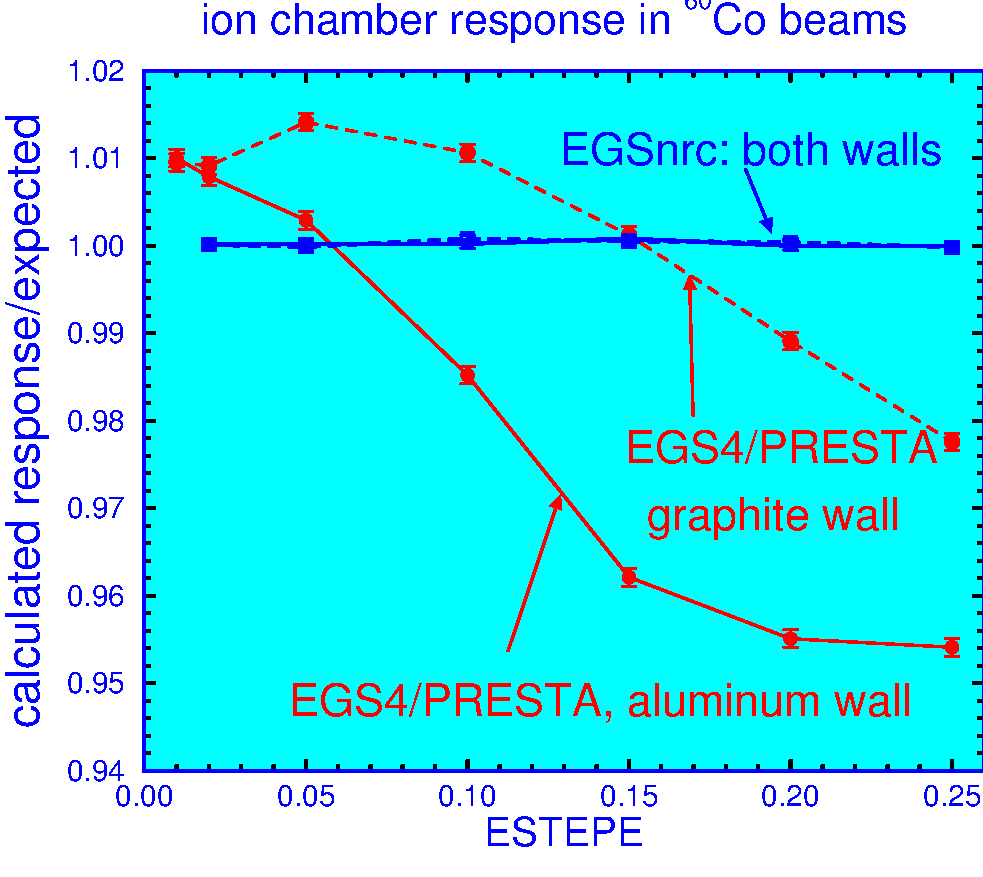
\includegraphics[height=10.5cm]{figures/ion_chamber}
%\caption{Improvement of EGSnrc compared to EGS4/PRESTA.}
%\cen{\Large Improvement of EGSnrc compared to EGS4/PRESTA.}
\end{center}
\end{figure}
\vfill

\copyright NRC Canada, 2001--2021
\end{center}
\newpage   %Blank page behind cover
\mbox{}


\newpage
\setlength{\baselineskip}{0.5cm}

\pagestyle{fancy}
\pagenumbering{arabic}
\setcounter{page}{1}


%%%%%%%%%%%%%%%%%%%%%%%%%%%%%%%%%%%%%%%%%%%%%%%%%%%%%%%%%%%%%%%%%%%%%%%%%%%%%%%
%
%  EGSnrc manual: preface
%  Copyright (C) 2015 National Research Council Canada
%
%  This file is part of EGSnrc.
%
%  EGSnrc is free software: you can redistribute it and/or modify it under
%  the terms of the GNU Affero General Public License as published by the
%  Free Software Foundation, either version 3 of the License, or (at your
%  option) any later version.
%
%  EGSnrc is distributed in the hope that it will be useful, but WITHOUT ANY
%  WARRANTY; without even the implied warranty of MERCHANTABILITY or FITNESS
%  FOR A PARTICULAR PURPOSE.  See the GNU Affero General Public License for
%  more details.
%
%  You should have received a copy of the GNU Affero General Public License
%  along with EGSnrc. If not, see <http://www.gnu.org/licenses/>.
%
%%%%%%%%%%%%%%%%%%%%%%%%%%%%%%%%%%%%%%%%%%%%%%%%%%%%%%%%%%%%%%%%%%%%%%%%%%%%%%%
%
%  Author:          Iwan Kawrakow, 2003
%
%  Contributors:    Blake Walters
%                   Frederic Tessier
%                   Ernesto Mainegra-Hing
%
%%%%%%%%%%%%%%%%%%%%%%%%%%%%%%%%%%%%%%%%%%%%%%%%%%%%%%%%%%%%%%%%%%%%%%%%%%%%%%%


\newpage
\mbox{ }\vspace*{-35mm}\\
\section*{\begin{center}Preface\end{center}}
\addcontentsline{toc}{section}{\numberline{}Preface}
\index{preface}
% Replace commented line for the one with fixed date when commiting
% Beware: Using the macro below conflicts between CVS and latex!!!
% \lfoot[{\sffamily {\leftmark}}]{{\small Last edited $Date: 2013/01/04 15:08:41 $
\lfoot[{\sffamily {\leftmark}}]{{\small Last edited 2011/05/02 18:36:27
}}
\mbox{ }\vspace*{-5mm}\\
\noindent {\bfseries Sixth printing: May 2011}\\
A long time has passed since the last update to this document.
Although no fundamental changes have been made to the system,
there have been a number of important additions and improvements
to the system since 2009. Numerous bugs have been corrected and
a new user code for free-air chamber (FAC) correction calculations
was added to the distribution.
\begin{itemize}
\item Use of arbitrary electron impact ionization (EII)
cross section compilations. Added a data base of EII
cross sections based on the DWBA/PWBA theory by
Bote and Salvat.
\item For backward compatibility with previous calculations, users can
now request the use of PEGS4 photon data.
\item Inclusion of C++ {\tt egs\_fac} application with example.
This user-code implements a self-consistent algorithm for the
fast calculation of FAC correction factors.
\item EII cross sections printout for materials in
  the simulation if user requests output of the photon cross-sections.
\item Updated several GUI's to include most of the latest additions
and corrected several bugs.
\end{itemize}
% \vspace{3mm}\\
\noindent {\bfseries Fifth printing: July 2009}\\
There has been a huge number of changes in the system since
the last printing in November 2003 that have not been properly
added to the documentation. This printing is an attempt to update
this report to better reflect the state of EGSnrc, although it
is far from complete. The development of the EGSnrc C++ class
library, which includes a general purpose geometry package, and its
first public release in 2005 has been a major step forward.
The C++ class library is described in a separate report (PIRS--898).
Major changes and additions to the EGSnrc physics include:
option to simulate electron impact ionization, an improved
bremsstrahlung data base that includes an exact evaluation of
electron-electron bremsstrahlung in the first Born approximation,
an improved differential pair production cross section tabulation
based on exact PWA calculations that takes into account the asymmetry
of the energy distribution at energies close to the threshold,
the ability to explicitely
simulate triplet interactions (\ie, pair production in the electron field),
the ability to take into account radiative corrections for Compton
scattering in the one-loop approximation, the ability to use
user-supplied atomic and molecular form factors for Rayleigh scattering,
and the ability to use total photon cross sections from EPDL97, XCOM, or
any other user-supplied tabulation in addition to the default
Storm \& Israel tabulations.
New options added for Compton scattering called {\tt simple} and
{\tt norej}. When using {\tt simple} binding is taken
into account via an incoherent scattering function
ignoring Doppler broadening. The incoherent scattering function
is still obtained from the impulse approximation.
The {\tt norej} option uses actual bound Compton cross section
when initializing the photon cross sections and rejections in
subroutine COMPT lead to re-sampling rather than rejecting the
entire interaction.
An {\tt alias sampling} algorithm is now used to select the
photon angle after a Rayleigh scattering to avoid an undersampling
at large angles observed in the original EGS4 implementation.
Particle track scoring object added to the {\tt egspp} library
allowing visualization of particle tracks with the C++ geometry
viewer {\tt egs\_view}. See example input file tracks1.egsinp for
the tutor7pp C++ user-code.

Finally, to better reflect their contributions
to the development and maintenence of the system, Ernesto Mainegra-Hing,
Blake Walters and Frederic Tessier have been added as co-authors.
\vspace{3mm}\\
\noindent {\bfseries Fourth printing: November 2003}\\
Added references to EGSnrcMP and Report PIRS-877. A few minor changes
related to the major change in the operating system to make it Windows
compliant. There is no associated change in the physics of the system.
Table 7 re timing of random numbers has changed substantially.
\vspace{3mm}\\
\noindent {\bfseries Third printing: April 2002}\\
Minor changes reflecting code changes.
%See section~\ref{fixed_bugs}.
\vspace{3mm}\\
\noindent {\bfseries Second printing: May 2001}\\
The second printing contains a description of the use of {\tt RHOF}
(section~\ref{RHOF_RHOR}, page~\pageref{RHOF_RHOR}) and {\tt \$SET-RHOF}
(section~\ref{set_rhof}, page~\pageref{set_rhof}). There is a brief new
discussion of {\tt combine\_egsnrc}, a script for automatic analysis of the
many files created by {\t pprocess} in parallel runs
((section~\ref{pprocess}, page~\pageref{pprocess})). There is a new section
about terminating histories with WT=0.0 (section~\ref{termination},
page~\pageref{termination}).
%Finally, a new section
%has been added which documents the few minor changes made to EGSnrc since
%its initial release ((section~\ref{fixed_bugs},
%page~\pageref{fixed_bugs})).
\vspace{3mm}\\
\noindent {\bfseries First printing: May 2000}\\
In the decade and a half since the original version of EGS4 was released
there have been well over 1000 papers published which cite the original
SLAC-265 Report.  The code itself has been improved in many different ways
by a large number of people.  For a detailed history of much of this up to
1994, the reader is referred to a report titled  ``History, overview and
recent improvements of EGS4'' by Bielajew et al.
\index{Bielajew, Alex}

In the last few years there have been significant advances in several
aspects of electron transport.  For example, improvements in multiple scattering
theory have been developed by Kawrakow and Bielajew\cite{KB97,Bi96,Ka96}
which get over most of
the shortcomings of the Moliere theory used in EGS4. Perhaps more important
has been the development by Kawrakow and Bielajew\cite{KB97a} of a new electron transport algorithm, sometimes
called PRESTA-II, which makes a significant advance in the science of
electron transport.  In addition to these advances, Kawrakow has implemented
several other improvements in the electron transport algorithm of EGS
which make it capable of accurately calculating ion chamber response at the
0.1\% level (relative to its own cross sections)\cite{Ka99a,Ka99b}.

EGSnrc also has implemented a variety of additional features, many of
which have previously been extensively developed as additions to EGS4
by  Namito, Hirayama and Ban at KEK as well\cite{Na98,Na95a,Na94,Na93}.
The EGSnrc approach differs from that of the KEK group, partially because
once we were making fundamental changes to the code, we carried it through
in a consistent manner. However, the KEK group have implemented several
options which are not yet in EGSnrc (e.g.  polarized photon scattering
and electron impact ionization).
\index{Hirayama, Hideo} \index{Namito} \index{Ban}

This report is meant to document the many changes that have occurred going
from EGS4 to EGSnrc.  Although this report is written by two people,
the EGS system is obviously the child of many parents who have made a
wide variety of contributions over the years.  This goes right back to
Richard Ford, then at SLAC, who was a major contributor to EGS3. Hideo
Hirayama, S Ban  and Yosh Namito of KEK have made innumerable contributions
to EGS, especially concerning the low energy photon physics. Alex
Bielajew worked on EGS at NRC from the early 80's to late 90's and his
name is linked to a huge number of important contributions to EGS,
perhaps most importantly the PRESTA algorithms, but also many other
specific improvements to the physics, the Unix based scripts and the NRC
user codes. His name appears very extensively in the reference lists.
The name of Walter Ralph Nelson is practically synonymous with EGS and
all users of any version of the EGS system will forever be in Ralph's
debt. It has been his enthusiasm and willingness to help others and share
this resource so selflessly which has made it the great success it is.
To all of these people who have contributed so extensively to the EGS
system, and to the countless others who have played a variety of roles,
we all owe a huge debt of gratitude.
\index{Nelson, Ralph}


It is worth noting that NRC and SLAC have drawn up a formal agreement which
recognizes that both have rights associated with EGS4 and EGSnrc.  Thus, in
this report there are sections which are taken verbatim from SLAC-265 (in
particular the PEGS4 manual and the User's guide to Mortran3) and we wish
to thank SLAC for permission to reproduce them.  We also draw attention to
the copyright and licensing arrangements associated with EGSnrc which are
similar to those for EGS4, but which are becoming more tightly controlled
in this changing world we live in.  Neither EGS4 nor EGSnrc are public
domain software. They are both copyright protected by NRC and/or SLAC. The
formal license statement is more precise and part of the package, but the
general meaning is that individuals are granted a without cost
license to use it for non-commercial purposes but that a license from NRC
is needed for any commercial application, and by definition someone working
for a for-profit organization or working on a contract for such an
organization is working on a commercial application.
\index{SLAC}


\noindent{\em What is next?\\}
In the section of the Preface to SLAC-265, there were 7 areas identified as
needing more work.  The work on EGS is not  complete, and at least 2 of
the 7 are still open, viz:
\begin{itemize}
\vspace{-4mm}
\item development of an efficient, general purpose geometry package
tailored to the EGS structure
\vspace{-3mm}
\item implementation of a general purpose energy loss straggling algorithm
which properly handles energy cutoffs
\end{itemize}

\vspace{-5mm}
There are other issues which are still undone within EGSnrc:
\vspace{-5mm}
\begin{itemize}
\item modeling of electron impact ionization
\vspace{-3mm}
\item some critical feature for your next application!!
\end{itemize}
We encourage users to contribute their improvements to the code. We will
happily add those which are of general interest and make available on the
distribution site those additions which are of special interest. We will
also appreciate receiving bug reports. Although we have done extensive QA
on the system, there have been many changes and not all parts of the code
are as carefully checked as we would like.  However, the pressure to release
the code is forcing us to proceed at this point.

We wish to thank our many colleagues at NRC who have helped with this work.
In particular Michel Proulx for his excellent help keeping the computer
systems going smoothly, Jan Seuntjens for his help with the user codes,
Joanne Treurniet for her help with the most recent version of the
EGS\_Windows system and Blake Walters for his work on QA of the system.

\noindent I.K and D.W.O.R.  \hfill Feb 2000 \vspace{1mm}\\

%\noindent {\bfseries Second printing: May 2001}\\
%The second printing contains a description of the use of {\tt RHOF}
%(section~\ref{RHOF_RHOR}, page~\pageref{RHOF_RHOR}) and {\tt \$SET-RHOF}
%(section~\ref{set_rhof}, page~\pageref{set_rhof}). There is a brief new
%discussion of {\tt combine\_egsnrc}, a script for automatic analysis of the
%many files created by {\t pprocess} in parallel runs
%((section~\ref{pprocess}, page~\pageref{pprocess})). There is a new section
%about terminating histories with WT=0.0 (section~\ref{termination},
%page~\pageref{termination}). Finally, a new section
%has been added which documents the few minor changes made to EGSnrc since
%its initial release ((section~\ref{fixed_bugs},
%page~\pageref{fixed_bugs})). \vspace{3mm}  \\
%\noindent {\bfseries Third printing: April 2002}\\
%Minor changes reflecting code changes. See section~\ref{fixed_bugs}.
%\vspace{3mm}\\
%\noindent {\bfseries Fourth printing: November 2003}\\
%Added references to EGSnrcMP and Report PIRS-877. A few minor changes
%related to the major change in the operating system to make it Windows
%compliant. There is no associated change in the physics of the system.
%Table 7 re timing of random numbers has changed substantially.
%\vspace{3mm}\\
%\noindent {\bfseries Fifth printing: July 2009}\\
%There has been a huge number of changes in the system since
%the last printing in November 2003 that have not been properly
%added to the documentation. This printing is an attempt to update
%this report to better reflect the state of EGSnrc, although it
%is far from complete. The development of the EGSnrc C++ class
%library, which includes a general purpose geometry package, and its
%first public release in 2005 has been a major step forward.
%The C++ class library is described in a separate report (PIRS--898).
%Major changes and additions to the EGSnrc physics include:
%option to simulate electron impact ionization, an improved
%bremsstrahlung data base that includes an exact evaluation of
%electron-electron bremsstrahlung in the first Born approximation,
%an improved differential pair production cross section tabulation
%based on exact PWA calculations that takes into account the asymmetry
%of the energy distribution at energies close to the threshold, the ability to explicitely
%simulate triplet interactions (\ie, pair production in the electron field),
%the ability to take into account radiative corrections for Compton
%scattering in the one-loop approximation, the ability to use
%user supplied atomic and molecular form factors for Rayleigh scattering,
%and the ability to use total photon cross sections from EPDL97, XCOM, or
%any other user-supplied tabulation in addition to the default
%Storm \& Israel tabulations. Finally, to better reflect their contributions
%to the development and maintenence of the system, Ernesto Mainegra-Hing,
%Blake Walters and Frederic Tessier have been added as co-authors.



\newpage

\tableofcontents

\newpage
\listoffigures
%\newpage
\listoftables

\setlength{\baselineskip}{0.5cm}

\newpage
%%%%%%%%%%%%%%%%%%%%%%%%%%%%%%%%%%%%%%%%%%%%%%%%%%%%%%%%%%%%%%%%%%%%%%%%

%		Introduction

%%%%%%%%%%%%%%%%%%%%%%%%%%%%%%%%%%%%%%%%%%%%%%%%%%%%%%%%%%%%%%%%%%%%%%%%

\renewcommand{\leftmark}{{1: Introduction}}
\typeout{Starting ``Introduction'' Should be on odd page}

%%%%%%%%%%%%%%%%%%%%%%%%%%%%%%%%%%%%%%%%%%%%%%%%%%%%%%%%%%%%%%%%%%%%%%%%%%%%%%%
%
%  EGSnrc manual: introduction
%  Copyright (C) 2015 National Research Council Canada
%
%  This file is part of EGSnrc.
%
%  EGSnrc is free software: you can redistribute it and/or modify it under
%  the terms of the GNU Affero General Public License as published by the
%  Free Software Foundation, either version 3 of the License, or (at your
%  option) any later version.
%
%  EGSnrc is distributed in the hope that it will be useful, but WITHOUT ANY
%  WARRANTY; without even the implied warranty of MERCHANTABILITY or FITNESS
%  FOR A PARTICULAR PURPOSE.  See the GNU Affero General Public License for
%  more details.
%
%  You should have received a copy of the GNU Affero General Public License
%  along with EGSnrc. If not, see <http://www.gnu.org/licenses/>.
%
%%%%%%%%%%%%%%%%%%%%%%%%%%%%%%%%%%%%%%%%%%%%%%%%%%%%%%%%%%%%%%%%%%%%%%%%%%%%%%%
%
%  Author:          Iwan Kawrakow, 2003
%
%  Contributors:    Blake Walters
%                   Frederic Tessier
%                   Ernesto Mainegra-Hing
%
%%%%%%%%%%%%%%%%%%%%%%%%%%%%%%%%%%%%%%%%%%%%%%%%%%%%%%%%%%%%%%%%%%%%%%%%%%%%%%%


\section{Introduction}
% Replace commented line for the one with fixed date when commiting
% Beware: Using the macro below conflicts between CVS and latex!!!
% \lfoot[{\sffamily {\leftmark}}]{{\small Last edited $Date: 2011/05/02 18:40:33 $
\lfoot[{\sffamily {\leftmark}}]{{\small Last edited 2011/05/02 18:36:27
}}
\subsection{Intent of this report}

\index{intent of report}
\index{purpose of report}
\index{acronym}
The EGS ({\bfseries E}lectron--{\bfseries G}amma--{\bfseries S}hower) system of computer codes is a general purpose package
for the Monte Carlo simulation of the coupled transport of electrons and
photons in an arbitrary geometry for particles with energies above a few
keV up to several hundreds of GeV.  This report introduces a new, enhanced version
called EGSnrc. In addition to explaining and documenting the various
enhancements and changes to the previous version (EGS4\cite{Ne85}),
this document includes several introductory and advanced tutorials
on the use of EGSnrc (section~\ref{tutorials}) and also contains
the \underline{EGSnrc Reference Manual}(section~\ref{ERM}),
the \underline{PEGS4 User Manual} (section~\ref{pegs4}), and
an \underline{EGS User Guide to Mortran3} (section~\ref{UGM3}).
Our intention has been to make this document wholly self-contained so
that the user need not refer to the original EGS4 User Manual\cite{Ne85}
although it is on-line and available at \htmladdnormallink{ {\sf
http://www.slac.stanford.edu/pubs/slacreports/slac-r-265.html}}
{http://www.slac.stanford.edu/pubs/slacreports/slac-r-265.html}.
The heart of the present report is Section 2 which documents the physics
in EGSnrc. This has changed substantially from the EGS4 comparable Chapter
2 because of the many changes in EGSnrc. However, we have chosen not to
repeat the general introduction to sampling and probability theory that
was in Chapter 2 of SLAC-265.

For a basic introduction to the code, see the reference manual,
section~\ref{ERM} (page~\pageref{ERM}).

\index{comparison to experiment}
We have not presented any comparisons with experiment in this
document since it has become such an extensive field that we have no
hope of reproducing a fraction of the data. Instead, we have prepared
a separate report on QA which presents extensive comparisons between
EGS4 and EGSnrc\cite{Wa00}. There are
significant differences in many situations because of the improved physics
in EGSnrc.  Two papers\cite{Ka99a,Ka99b} discuss many
of the details of the new physics, especially as related to ion chamber
calculations (which are perhaps the toughest test of any electron-photon
Monte Carlo transport code).  These papers provide analytic models which
explain many of the shortcomings of the EGS4/PRESTA system in this very
difficult problem.  The cover of this report shows a 
comparison of the two codes run in their standard default modes.
\index{ion chamber calculations}

\subsection{History of the EGS system}
\index{history}
\index{Bielajew, Alex}
The history has already been outlined in the Preface. For a detailed
history up to
1994, the reader is referred to a report titled  ``History, overview and
recent improvements of EGS4'' by Bielajew et al. That
report draws heavily on the history sections of the 
SLAC-210\cite{FN78} and SLAC-265\cite{Ne85} reports with an update to
1994.

As stated in the Preface, EGSnrc is the child of many parents who have
made a wide variety of contributions over the years. We will not repeat
the preface here except to note that Walter ``Ralph'' Nelson has been
the key player in the development of the system over the years and we
all owe him a debt of gratitude.
\index{Nelson, Ralph}


\subsection{Summary of EGSnrc Capabilities and Features}
\index{EGSnrc!summary capabilities}
\index{capabilities of EGSnrc}
\index{EGSnrc!features}
\index{features of EGSnrc}

The following is a summary of the main features of the EGSnrc
Code System, including statements about the physics that
has been put into it and what can be realistically simulated.

\begin{itemize} 
\item The radiation transport of electrons ($+$ or $-$) or photons
can be simulated in any element, compound, or mixture.  
The data preparation package, PEGS4, creates data to be used by
EGSnrc, using cross section tables for elements 1 through 100. In addition
there are other data files which must be read in to implement many of the
new options.

\item Both photons and charged particles are transported in
steps of random length rather than in discrete steps.

\index{low energy limit!electron}
\index{low energy limit!photon}
\item The dynamic range of charged particle kinetic energies
goes from a few tens of keV up to a few hundred GeV.  Conceivably
the upper limit can be extended higher, but the validity of the
physics remains to be checked.

\index{allowed energy range}
\index{energy range}
\item The dynamic range of photon energies lies between 1 keV and
several hundred GeV (see above statement).

\item The following physics processes are taken into account
by the EGSnrc Code System:

\index{physics processes in EGSnrc}
\index{EGSnrc!physics processes}
\begin{itemize} 
  \item Bremsstrahlung production using either Bethe-Heitler cross sections
or the NIST cross sections.

  \item Positron annihilation in flight and at rest
  (the annihilation quanta are followed to completion).

  \item Multiple scattering of charged particles by coulomb scattering from
nuclei is handled using a new
multiple scattering theory which overcomes the shortcomings of Moli\`ere 
multiple scattering theory. It allows for steps of any size and
moves seamlessly from a single scattering
model for short steps to an  accurate multiple scattering model
at large steps.  The user has the option of scattering based on
Rutherford scattering or scattering accounting for relativistic and spin
effects.

  \item M\o ller ($e^-e^-$) and Bhabha ($e^+e^-$) scattering.
  Exact rather than asymptotic formulae are used.

  \item Continuous energy loss applied to charged particle
  tracks between discrete interactions.
    \begin{itemize} 
    \item Total restricted charged particle stopping power consists of 
    soft bremsstrahlung and collision loss terms.
     
    \item Collision loss determined by the restricted
    Bethe-Bloch stopping power with Sternheimer treatment of
    the density effect in the general case but with provision of using
    an arbitrary density effect correction and data supplied to use the
    density effect recommended by the ICRU in Report 37.
    \end{itemize} 

  \item Pair production.
   
  \item Compton scattering, either Klein-Nishina or bound Compton.
   
  \item Coherent (Rayleigh) scattering can be included
  by means of an option.
   
  \item Photoelectric effect.
    
  \item Relaxation of excited atoms after vacancies are created (eg after
      photoelectric or Compton scattering events) to create fluorescent photons 
     (K, L, M shells) and Auger and Coster-Kronig
     electrons may be produced and tracked if requested.

  \item Electron impact ionization can be modeled using arbitrary theories
        for generating cross-sections. Five such cross-section compilations 
        are provided in the EGSnrc distribution (Kawrakow, Casnati, 
        Kolbenstvedt, Gryzinski, and Bote and Salvat).

\end{itemize} 
 
\item PEGS4 is a stand-alone data preprocessing code consisting of
12 subroutines and 85 functions.  The output is in a
form for direct use by EGS4.
\begin{itemize} 
   
  \item PEGS4 constructs piecewise-linear fits over a large
  number of energy intervals of the cross section and branching
  ratio data.
   
  \item In general, the user need only use PEGS4 {\it once} to
  obtain the media data files required by EGSnrc.
   
  \item PEGS4 control input uses the NAMELIST read facility of
  the FORTRAN language (in Mortran3 form).
   
  \item In addition to the options needed to produce data for
  EGSnrc, PEGS4 contains options to plot any of the physical
  quantities used by EGSnrc.
 
  \item In addition to the material specific data files produced by PEGS4,
   EGSnrc uses a variety of other data files as input for the calculations.
\end{itemize} 
 
\item EGSnrc is a package of subroutines plus block data with
a flexible user interface.
   
  \begin{itemize} 
  \item This allows for greater flexibility without requiring
  one to be overly familiar with the internal details of the code.
   
  \item Together with the macro facility capabilities of the
  Mortran3 language, this reduces the likelihood that user edits
  will introduce bugs into the code.
   
  \item EGSnrc uses material cross section and branching ratio
  data created and fit by the companion code, PEGS4. However,
  photon cross-section data are re-calculated on-the-fly
  using a logarithmic energy grid with an user-specific number
  of interpolation points. This behaviour can now be reverted
  if the user so desires.
 
\index{EGSnrc!geometry}
\item The geometry for any given problem is specified by a
{\it user-written} subroutine called HOWFAR which, in turn,
can make use of auxiliary subprograms.
   
  \item Auxiliary geometry routines for planes, cylinders,
  cones, spheres, etc., are provided with the EGSnrc Code System
  for those who do not wish to write their own.
   
  \item Macro versions of these routines are also provided in the
  set of defining macros (\ie, in the {\tt egsnrc.macros} file) which,
  if used, generally result in a faster running simulation.
   
   
\index{magnetic field transport}
\index{electric field transport}
  \item Transport can take place in a magnetic field by writing
  a specially designed HOWFAR subprogram, or in a more general
  manner (\eg, including electric field) by making use of
  Mortran3 macro templates that have been appropriately placed
  for that purpose in subroutine ELECTR.The file {\tt emf\_macros.mortran}
  contains Bielajew's macros to implement this.
   \index{emf\_macros.mortran}
   \index{Bielajew, Alex}
  \end{itemize} 
 
\item The user scores and outputs information in the
{\it user-written} subroutine called AUSGAB.
   
  \begin{itemize} 

  \item By setting various {\tt AUSFLG} flags, the user can arrange to have
access to the simulation parameters under many different situations to
allow scoring of almost any parameter of interest with out delving into the
code itself.

  \item Auxiliary subprogram WATCH is provided in order to allow
  an event-by-event or step-by-step tracking of the simulation, either to
the terminal or for 3-D graphics display using the program EGS\_Windows.
 \end{itemize} 
 
\item EGSnrc allows for the implementation of {\it importance
sampling} and other variance reduction techniques (\eg, leading
particle biasing, splitting, path length biasing, Russian
roulette, etc.). 
  \begin{itemize} 
  \item EGSnrc introduces options to allow for efficient bremsstrahlung 
    splitting and Russian Roulette of secondary charged-particles, but only 
    if ``turned on'' by the user.
  \item EGSnrc calculates the range and distance of the particle to the
   nearest boundary on every step as part of the electron transport algorithm
   and there is an option to do range rejection on any particle that cannot get out of
   the current region.
 
\end{itemize} 

\item Initiation of the radiation transport:
   
\begin{itemize} 
  \item An option exists for initiating a shower with two
  photons from pi-zero decay (\ie, use $IQI=2$ in the
  {\tt CALL SHOWER} statement). 
   
  \item The user has the choice of initiating the transport
  by means of a monoenergetic particle, or by sampling from
  a known distribution (\eg, a synchrotron radiation spectrum).
   
  \item Transport can also be initiated from sources that have
  spatial and/or angular distributions.

  \end{itemize} 
\end{itemize} 


\newpage
\subsection{Summary of changes from EGS4}
\label{changes_summary}
\index{changes from EGS4}
\index{EGS4}
\index{EGS4!changes from}
This is a brief listing of these changes which are discussed more fully in
section~\ref{section_2} and in section~\ref{changes}.

\subsubsection{Physics changes}

\begin{itemize} 
\item A completely new electron transport algorithm is used which removes
all known shortcomings of the EGS4/PRESTA algorithm.  If the geometry
permits, the new algorithm can take much larger steps with better accuracy
than previously. As it crosses a boundary, it goes into single scattering
mode to ensure an accurate boundary crossing. The EGS4/PRESTA algorithm
is still available as an option.

\item A new multiple scattering theory is used which gets around the
shortcomings of Moliere multiple scattering theory. It seamlessly goes from
a single scattering mode for short steps to a multiple scatter mode for
long steps.

\item Within the new multiple scattering theory an option has been added to
include relativistic spin effects in the cross section instead of just the
Rutherford cross section which underlies Moliere theory.

\item If desired, it is possible to do the entire calculation modeling
elastic scattering in a single scattering mode. This is at the cost of a
great deal of computing time and also does not model the inelastic energy
losses in a single scattering model.

\item A relaxation simulation feature has been added which allows creation
and following of fluorescent photons from K, L, M shells, Auger electrons and
Coster-Kronig electrons. Currently this can be called after photo-electric
and Compton scattering events.

\item If relaxation is not being modeled, then a photo-electron in EGSnrc
carries the entire energy of the incident photon. This is a better
approximation in most cases than dumping the binding energy locally and
subtracting the binding energy from the photo-electron's energy (as done in
EGS4).

\item Sampling the angular distribution of the photo-electron is available
as an option.

\item Bound Compton scattering can be simulated as well as Klein-Nishina
Compton scattering.

\item Bremsstrahlung angular sampling has been changed from a fixed angle
approximation to allowing the angular distribution to be sampled in one of
two ways.

\item A bug was fixed in the bremsstrahlung photon energy sampling routine
which affected simulations for which AP was not small relative to the electron
energy.  Doing this led to a complete rewrite of the sampling routine which
also increased its efficiency.

\item A second bremsstrahlung photon energy sampling option was added which 
uses the more accurate NIST differential cross sections.

\item PEGS4 has been modified to pick up the data files which scale the
radiative cross sections to produce the NIST/ICRU 37 radiative stopping
powers.

\item A variety of variance reduction techniques which were commonly used
with EGS4 have been ``built in'' with EGSnrc to improve the efficiency
   \begin{itemize} 
   \item bremsstrahlung splitting is done within the routine BREMS, thereby
         avoiding repeatedly calculating several constants
   \item Russian Roulette of secondary charged particles is done in a
         manner which sometimes avoids sampling the particles phase space unless
         it survives.
   \item range rejection, viz the termination of a particle history, when
         it cannot escape the local region, is implemented naturally and
         very efficiently since the particle range and distance to the
	 nearest boundary are already calculated on every step.
   \end{itemize}

\item Subroutine HATCH has been modified considerably to allow
initialization for the many new options.

\item The Moller sampling routine was corrected as first done in the
1997 release of EGS4.


\item The efficiency of the annihilation sampling routine has been
improved.

\item The sampling of the azimuthal angle has been recoded and saves a
noticeable amount of time in a real calculation (2\% in one example).

\item Various changes have been made in the COMIN blocks to accommodate the
above changes. Also LATCH and LATCHI are  now a default part of STACK. 

\item Several more AUSGAB calls are available to score Auger
and Coster-Kronig electrons and fluorescent x-rays.

\end{itemize} 



\subsubsection[System changes]{System changes pre-EGSnrcMP(see
ref\cite{Ka03} for the MP changes)}
\index{EGSnrc!system changes}
\begin{itemize} 

\item The various source files have been rationalized and various add-on
features to EGS4 have been made part of EGSnrc.

\index{ranmar} \index{ranlux} \index{parallel processing}
\item Two options for random number generator are available. The
default is the RANLUX generator which allows various ``luxury levels''
of generator to be used and the RANMAR generator, which had become the
standard for the Unix distribution of EGS4, is also available, although
re-coded.  Both generators have the ability to generate sequences which
are known to be independent and thus can be used for parallel processing.
At the default luxury level of 1, the RANLUX generator is slightly slower
than the recoded RANMAR generator, but the difference has a negligible
impact on overall computing time.

\item The default for calculating sines is now a function call because
modern machines do this very rapidly and the table lookup method is known
to be inaccurate for very small angles.

\item The EGS\_Windows code for generating  3-D interactive displays has
been ported to run on any X-windows platform using non-proprietary
software.

\item The entire code has been written using {\tt IMPLICIT NONE}. Further,
all declarations have been done using {\tt \$REAL} and {\tt \$INTEGER}
constructs which allow conversion to running double precision by redefining
2 macros, as long as the user codes  do the same thing!

\item Subroutine WATCH has been modified to accommodate the changes in the
physics.

\end{itemize} 

\subsubsection{User code changes}
\index{User codes}

\begin{itemize} 
\item The tutor codes have been rewritten to work with EGSnrc and a new
version of tutor6 has been written to demonstrate control of all variables
available to EGSnrc users.

\item Four of the standard NRC user codes for cylindrical geometry problems
 are now distributed with the system, DOSRZnrc, FLURZnrc, CAVRZnrc and
SPRRZnrc.

\item The above user codes have been extensively reworked to use a
new generalized input package which makes it much easier for the user
to generate the input files since the inputs are text oriented. Also,
the geometry and physics transport inputs are common for all codes.

\item The output routines have been reworked to avoid the use of
VAX extensions to Fortran which were not available with many Unix compilers.

\item The user codes have been cleaned up to some extent although not as
much as desirable! The main user codes systematically use {\tt
\$IMPLICIT-NONE}
and {\tt \$REAL, \$INTEGER} constructs to allow compatibility with EGSnrc and
the ability to change to double precision at will.

\item a bug in the energy sampling routine which caused problems in some
cases has been removed. An entirely new code which is faster and more
accurate is used now.
\end{itemize} 

\subsection{Summary of changes since 2005 edition of this report}

\subsubsection{Physics changes since 2005} 

\begin{itemize}

  \item Electron impact ionization can be modeled using four different theories
        for generating cross-sections (Kawrakow, Casnati, Kolbenstvedt, or
        Gryzinski).

  \item The user has the option of supplying custom molecular form factors
        when including Rayleigh scattering in a simulation.

  \item New {\tt alias sampling} algorithm used to select the 
        photon angle after a Rayleigh scattering.

  \item New options added for Compton scattering called {\tt simple} and 
        {\tt norej}.

  \item The user has the option to include radiative corrections for Compton
        scattering.

  \item The user has the option to use exact PWA cross sections for pair 
        production

  \item The user has the option to explicitely simulate triplet production

  \item A new bremsstrahlung data base has been added that incorporates a much 
        improved evaluation of electron-electron bremsstrahlung

  \item The ability to use total photon cross sections from EPDL-97, XCOM, 
        or any other user-supplied tabulation has been added


\end{itemize}

\subsubsection{ EGSnrc snapshots }

Since 2008 development snapshots of the EGSnrc system have been made 
available on the EGSnrc web page. These snapshots are updated much more 
regularly (typically every 2--8 weeks) but for now they can only be installed 
via a significantly simplified script on Linux systems with the GNU compilers. 

\subsubsection{User code changes since 2005}

\begin{itemize}

\item Two tutor codes, {\tt tutor2pp} and {\tt tutor7pp}, have been
added which make use of the C++ class library.  These codes are the
C++ equivalents to {\tt tutor2} and {\tt tutor7}.

\item Four new user codes which use the EGSnrc C++ class library have
also been added: 1) {\tt egs\_cbct} for simulating cone beam CT scans,
2) {\tt egs\_chamber} for efficient chamber simulations, 3) {\tt egs\_fac}
for simulating transport in a free-air chamber, and 4) {\tt egs\_pet} for
simulating PET scans, in addition to {\tt cavity}, the first major C++ code 
for EGSnrc released in 2005. Note that {\tt egs\_cbct} and {\tt egs\_pet} 
are not included in this public release.

\end{itemize} 

\subsection{Summary of changes since 2009 edition of this report}

There have been several additions to the physics 
and to the user codes available since the 
2009 edition of PIRS-701.  These are outlined in this section.

\subsubsection{Physics changes since 2009} 

\begin{itemize}

  \item A new electron impact ionization (EII) cross-section data base, 
        based on the DWBA/PWBA model by Bote and Salvat has been added
        to the distribution.

  \item The ability to use different EII cross section compilations
        has been generalized to allow the use of any user-supplied 
        tabulation.

  \item The user has the option of forcing the use of photon 
        cross-sections from the PEGS4 data file.

\end{itemize}

\subsubsection{ EGSnrc snapshots }

Since 2010 no snapshots of the EGSnrc system have been made 
available on the EGSnrc web page. The number of users making use
of this option is so small that it doesn't justify the effort put 
into creating them.

\subsubsection{User code changes since 2009}

The C++ user-code {\tt egs\_fac} has been finally included in the
distribution. This user-code simulates the transport in a 
free-air chamber and the calculations of correction factors
in a self-consistent manner. The user-codes {\tt egs\_cbct} 
and {\tt egs\_pet} are not included since they are in a very
experimental stage and not ready for public release.

\subsection{Outline of report}

In the remainder of this report there are 7 sections.  

Section 2 (page~\pageref{section_2}) presents a detailed description
of the physics in EGSnrc. While this section provides very important
documentation of what the code is doing, it is not essential reading in
order to get the code working.  Arguably it is essential reading before
you can use the code really well!

Section 3 (page~\pageref{ERM}) provides a detailed reference manual
which tells you what must be done to write your own user code.

Section 4 (page~\pageref{tutorials}) presents a series of short tutorial
programs which demonstrate the essential elements of EGSnrc user codes.
These are designed for those who learn by seeing examples (like DWOR).

Section 5 (page~\pageref{changes}) presents a summary of the changes
compared to EGS4 and a step by step procedure for upgrading an EGS4 user
code to work with EGSnrc.

Section 6 (page~\pageref{pegs4}) is the PEGS4 Users manual taken directly
from SLAC-265 along with a few additional pieces of documentation,
mostly about the upgrades since the original PEGS4 was released.

Section 7 (page~\pageref{UGM3}) is an EGS user guide to Mortran3, again
taken directly from SLAC-265.

Section 8 (page~\pageref{sys_consid}) outlines various system
considerations associated with running EGSnrc in a Unix environment. It
also discusses installation and distribution of the code.

We also draw your attention to the index which may help  find things.


\subsection{Associated documents}

%%%%%%%%%%%%%%%%%%%%%%%%%%%%%%%%%%%%%%%%%%%%%%%%%%%%%%%%%%%%%%%%%%%%%%%%%%%%%%%
%
%  EGSnrc manual: associated documents
%  Copyright (C) 2015 National Research Council Canada
%
%  This file is part of EGSnrc.
%
%  EGSnrc is free software: you can redistribute it and/or modify it under
%  the terms of the GNU Affero General Public License as published by the
%  Free Software Foundation, either version 3 of the License, or (at your
%  option) any later version.
%
%  EGSnrc is distributed in the hope that it will be useful, but WITHOUT ANY
%  WARRANTY; without even the implied warranty of MERCHANTABILITY or FITNESS
%  FOR A PARTICULAR PURPOSE.  See the GNU Affero General Public License for
%  more details.
%
%  You should have received a copy of the GNU Affero General Public License
%  along with EGSnrc. If not, see <http://www.gnu.org/licenses/>.
%
%%%%%%%%%%%%%%%%%%%%%%%%%%%%%%%%%%%%%%%%%%%%%%%%%%%%%%%%%%%%%%%%%%%%%%%%%%%%%%%
%
%  Author:          Iwan Kawrakow, 2003
%
%  Contributors:    Blake Walters
%                   Frederic Tessier
%                   Ernesto Mainegra-Hing
%
%%%%%%%%%%%%%%%%%%%%%%%%%%%%%%%%%%%%%%%%%%%%%%%%%%%%%%%%%%%%%%%%%%%%%%%%%%%%%%%

% Replace commented line for the one with fixed date when commiting
% Beware: Using the macro below conflicts between CVS and latex!!!
% \lfoot[{\sffamily {\leftmark}}]{{\small Last edited $Date: 2011/05/02 18:36:27 $
\lfoot[{\sffamily {\leftmark}}]{{\small Last edited 2011/05/02 18:30:41
}}

\index{associated documents}
There are a variety of papers which have been written about EGSnrc and
several NRC reports which are part of the distribution.  These are
listed below.  There are also a large number of papers which have been
written about EGS4.

\subsubsection{Refereed Papers}
\begin{itemize}
\item {\bfseries Accurate condensed history Monte Carlo simulation of
     electron transport. I. EGSnrc, the new EGS4 version:} \\
 I. Kawrakow, Medical Physics, {\bf 27} (2000) 485 -- 498.\\
Describes the overall implementation of the new electron transport
physics in EGSnrc.

\item {\bfseries Accurate condensed history Monte Carlo simulation of
     electron transport. II. Application to ion chamber response
     simulations:}\\
 I. Kawrakow, Medical Physics, {\bf 27} (2000) 499 -- 513.\\
Quantifies which problems in EGS4 led to the difficulties simulating ion
chamber response accurately and demonstrates that EGSnrc does not have
these problems.

\item {\bfseries Monte Carlo study of Spencer-Attix cavity theory at low
     photon energies:}\\
J. Borg, I. Kawrakow, D.W.O. Rogers and J.P.  Seuntjens, Med. Phys. {\bf
 27} (2000) 1804 -- 1813.
\\Uses code to explore the accuracy of Spencer-Attix cavity theory.
Paper demonstrates the accuracy of the EGSnrc code system for calculations
related to real ion chambers.


\item {\bfseries On the representation of electron multiple
elastic-scattering distributions for Monte Carlo calculations:}\\
I. Kawrakow and A. F.  Bielajew, Nucl. Inst. Meth. B 134, (1998) 325 --
336\\ Describes the multiple scattering theory used in EGSnrc.

\index{Bielajew, Alex}
\item {\bfseries On the condensed history technique for electron
transport:}\\
I. Kawrakow and A. F.  Bielajew, Nuclear Instruments and
Methods B 142 (1998) 253 -- 280.\\ Describes the electron transport
algorithm used in EGSnrc and demonstrates its improved accuracy compared
to all other published algorithms.


\end{itemize}
\subsubsection{Internal Reports}
\begin{itemize}
\item {\bfseries Monte Carlo calculated wall and axial non-uniformity
     corrections for primary standards of air kerma},\\
D. W. O.  Rogers and J. Treurniet, NRC Report PIRS--663, May 1999.\\Describes extensive EGSnrc
calculations of ion chamber response and comparison to experimental data
from standards labs of response vs wall thickness. Also notes that results
for these calculations, which are or correction factors, are the same as
for EGS4/PRESTA calculations.
\end{itemize}

\subsubsection{Manuals etc}

\begin{itemize}
\item {\bfseries NRC User Codes for EGSnrc}\\ D.W.O. Rogers, I. Kawrakow, J.P.
Seuntjens and B.R.B. Walters, NRC Report PIRS--702, May 2009.\\
Describes the EGSnrc user codes DOSRZnrc, CAVRZnrc, FLURZnrc and
SPRRZnrc as well as the generalized input routine developed for use with
EGSnrc user codes.

\item {\bfseries EGS\_Windows4.0 User's Manual},\\ J. A.  Treurniet and D.
W. O.  Rogers, NRC Report PIRS--669, Oct 1999.\\
Describes the latest version of  EGS\_Windows which works on any X-windows
based system and can be used to display EGSnrc histories in 3-D.\\


\item {\bfseries  QA tests and comparisons of the EGSnrc system
with EGS4},\\ B. R. B. Walters, J. Treurniet, D. W. O. Rogers
               and I. Kawrakow, NRC Report PIRS-703, March 2000.\\
Summarizes a large number of comparisons between EGS4 and EGSnrc to
highlight some differences and similarities.\\


\item {\bfseries  EGSnrcMP: the multi-platform environment for EGSnrc}, \\
I. Kawrakow, E. Mainegra-Hing and D. W. O. Rogers
           NRC Report PIRS-877, Sept 2006.\\
Describes the changes in the system of scripts used to run the EGSnrc
system. These major changes mean that EGSnrc now works under the Windows OS
and there are GUI's for installing and running the system.\\


\item {\bfseries egs\_inprz, a GUI for the NRC RZ user-codes}, \\
E. Mainegra-Hing, NRC Report PIRS-801, May 2005.\\
Manual for GUI for RZ user codes.\\


\item {\bfseries EGSnrc C++ class library},\\
I. Kawrakow, NRC Report PIRS-898, Apr 2006.\\
Manual describing the geometry and source modules available with the
EGSnrc C++ class library.  Also describes how to build a user code using
this library.  Includes descriptions of the C++ user codes, {\tt cavity},
{\tt egs\_chamber}, {\tt egs\_cbct}, {\tt egs\_fac} and {\tt egs\_fac}.\\

\end{itemize}




\clearpage

%%%%%%%%%%%%%%%%%%%%%%%%%%%%%%%%%%%%%%%%%%%%%%%%%%%%%%%%%%%%%%%%%%%%%%%%

%		Radiation Transport in EGSnrc

%%%%%%%%%%%%%%%%%%%%%%%%%%%%%%%%%%%%%%%%%%%%%%%%%%%%%%%%%%%%%%%%%%%%%%%%
\mbox{}\newpage		%needed to get next section on odd page

\renewcommand{\leftmark}{{2: Radiation transport in EGSnrc}}
\typeout{   Starting ``Radiation transport in EGSnrc''  Should be odd page}

%%%%%%%%%%%%%%%%%%%%%%%%%%%%%%%%%%%%%%%%%%%%%%%%%%%%%%%%%%%%%%%%%%%%%%%%%%%%%%%
%
%  EGSnrc manual: radiation transport
%  Copyright (C) 2015 National Research Council Canada
%
%  This file is part of EGSnrc.
%
%  EGSnrc is free software: you can redistribute it and/or modify it under
%  the terms of the GNU Affero General Public License as published by the
%  Free Software Foundation, either version 3 of the License, or (at your
%  option) any later version.
%
%  EGSnrc is distributed in the hope that it will be useful, but WITHOUT ANY
%  WARRANTY; without even the implied warranty of MERCHANTABILITY or FITNESS
%  FOR A PARTICULAR PURPOSE.  See the GNU Affero General Public License for
%  more details.
%
%  You should have received a copy of the GNU Affero General Public License
%  along with EGSnrc. If not, see <http://www.gnu.org/licenses/>.
%
%%%%%%%%%%%%%%%%%%%%%%%%%%%%%%%%%%%%%%%%%%%%%%%%%%%%%%%%%%%%%%%%%%%%%%%%%%%%%%%
%
%  Author:          Iwan Kawrakow, 2003
%
%  Contributors:    Blake Walters
%                   Ernesto Mainegra-Hing
%
%%%%%%%%%%%%%%%%%%%%%%%%%%%%%%%%%%%%%%%%%%%%%%%%%%%%%%%%%%%%%%%%%%%%%%%%%%%%%%%


\section{Radiation transport in EGSnrc}
\label{section_2}

%\subsection{General discussion}
\subsection{Introduction}
% Replace commented line for the one with fixed date when commiting
% Beware: Using the macro below conflicts between CVS and latex!!!
% \lfoot[{\sffamily {\leftmark}}]{{\small Last edited $Date: 2011/05/02 18:40:33 $
\lfoot[{\sffamily {\leftmark}}]{{\small Last edited 2011/05/02 18:32:38
}}


Photons interact with surrounding matter via four 
basic processes: materialization into an electron/positron pair 
in the electromagnetic field of the nuclei and surrounding 
atomic electrons, incoherent (Compton) scattering with 
atomic electrons, 
photo-electric absorption and 
coherent (Rayleigh) scattering with 
the molecules (or atoms) of the medium. The first three 
collision types transfer energy from the photon radiation 
field to electrons\footnote{In this report, we often refer to
both positrons and electrons as simply {\it electrons}.
Distinguishing features will be brought out in the context.}, 
one of them dominate depending on energy and the medium 
in which the transport takes place. The pair production 
process\footnote{Occasionally the materialization into an $e^+e^-$ pair 
takes place with the participation of an atomic electron which, after 
receiving sufficient energy, is set free. Such processes are known 
as triplet production.} dominates at high energies. 
At some intermediate energies incoherent scattering is the most 
important process, at low energies the photo-electric process 
dominates.

Electrons, as they traverse matter, lose energy by two basic processes:
inelastic collisions with atomic electrons and radiation. 
Radiative energy loss, which occurs in form of bremsstrahlung and 
positron annihilation, transfers energy back to photons 
and leads to the coupling of the electron and photon 
radiation fields. The bremsstrahlung process is the dominant 
mechanism of electron energy loss at high energies, inelastic collisions  
are more important at low energies. 
In addition, electrons participate in elastic collisions with atomic 
nuclei which occur at a high rate and lead to frequent changes 
in the electron direction. 

Inelastic electron collisions and photon interactions with atomic electrons 
lead to excitations and ionizations of the atoms along the paths of 
the particles. Highly excited atoms, with vacancies in inner shells, 
relax via the emission of photons and electrons with 
characteristic energies. 

The coupled integro-differential equations 
that describe the electromagnetic shower development are 
prohibitively complicated to allow for an analytical treatment 
except under severe approximations. The Monte Carlo (MC) technique 
is the only known solution method that can be applied for 
any energy range of interest. 

Monte Carlo 
simulations of particle transport processes are a faithful simulation
of physical reality: particles are ``born" according to distributions
describing the source, they travel certain distances, determined by a
probability distribution depending on the total interaction
cross section, to the site of a collision and scatter into
another energy and/or direction according to the corresponding
differential cross section, possibly producing new 
particles that have to be transported as well. 
This procedure is continued until all particles are 
absorbed or leave the geometry under consideration.
Quantities of interest can be calculated by averaging over a given set of
MC particle ``histories" (also refereed to as ``showers'' or 
``cases''). From mathematical points of view each particle 
``history'' is one point in a $d$-dimensional space (the dimensionality 
depends on the number of interactions) and the averaging procedure 
corresponds to a $d$-dimensional Monte Carlo integration. 
As such, the Monte Carlo estimate of quantities of interest 
is subject to a 
statistical uncertainty which depends on 
$N$, the number of particle histories simulated,   
and usually decreases as $N^{-1/2}$. Depending on the 
problem under investigation and the desired statistical 
accuracy, very long calculation times may be necessary. 

An additional difficulty occurs in the case of the Monte Carlo 
simulation of electron transport. In the process of slowing down, 
a typical fast electron
and the secondary particles it creates
undergo hundreds of thousands of interactions with
surrounding matter.  Because of this large number of collisions,
an event-by-event simulation of electron transport is often
not possible due to limitations in computing power.  To
circumvent this difficulty, Berger \cite{Be63} developed the
``condensed history" (CH) technique for the simulation 
of charged particle transport. In this method, large numbers of
subsequent transport and collision 
processes are ``condensed" to a single ``step''
The cumulative effect of the individual interactions is taken
into account by sampling the change of the particle's energy, 
direction of motion, and position, at the end of the step from appropriate
multiple scattering distributions.
The CH technique, motivated
by the fact that single collisions with the atoms cause, in most cases,
only minor changes in the particle's energy and direction of flight,
made the MC simulation of charged particle transport possible but introduced
an artificial parameter, the step-length. The dependence of the calculated
result on the step-length has become known as a step-size artifact
\cite{BR89}.

EGSnrc is a general purpose package for the Monte Carlo 
simulation of coupled electron and photon transport that 
employs the CH technique. 
It is based on the popular EGS4 system \cite{Ne85} 
but includes a variety of enhancements in the CH implementation 
and in some of the underlying cross sections. We recognize that many 
of the modifications that we have made to the original 
EGS4 implementation are not important for 
high energy applications, initially EGS4' primary target.   
On the other side, the energy range of application of the 
EGS4 system has shifted over the years to lower and lower 
energies. To facilitate this transition many enhancements 
to the original EGS4 implementation has been developed, 
{\em e.g.} the PRESTA algorithm \cite{BR87}, the 
inclusion of angular distribution of bremsstrahlung 
photons \cite{Bi89}, the low energy photon cross section 
enhancements by the group at KEK/Japan \cite{Na98}, to 
mention only some of them. The availability of these 
improvements, recent advances in the theoretical understanding 
of the condensed history technique \cite{KB97a,Ka99a} and 
multiple elastic scattering \cite{KB97}, as well as 
unpublished results of our recent research have 
motivated us to undertake a major re-work of the EGS4 
system the result of which is EGSnrc. 

It is the purpose of this report to summarize the current stage of the 
EGSnrc system. We have attempted a self-consistent presentation 
and so, some of the material contained in this report is 
not new. In particular, various parts come from the EGS4 manual, SLAC-265
by Nelson et al\cite{Ne85}.
\index{SLAC-265}
\index{Nelson, Ralph} 

This report does not attempt to provide a complete treatment of Monte 
Carlo methods or probability and sampling theory. 
Readers not familiar with the Monte Carlo technique are encouraged to   
read one of the many excellent reviews available.  


%%%%%%%%%%%%%%%%%%%%%%%%%%%%%%%%%%%%%%%%%%%%%%%%%%%%%%%%%%%%%%%%%%%%%%%%%%%%%%%
%
%  EGSnrc manual: photon interactions
%  Copyright (C) 2015 National Research Council Canada
%
%  This file is part of EGSnrc.
%
%  EGSnrc is free software: you can redistribute it and/or modify it under
%  the terms of the GNU Affero General Public License as published by the
%  Free Software Foundation, either version 3 of the License, or (at your
%  option) any later version.
%
%  EGSnrc is distributed in the hope that it will be useful, but WITHOUT ANY
%  WARRANTY; without even the implied warranty of MERCHANTABILITY or FITNESS
%  FOR A PARTICULAR PURPOSE.  See the GNU Affero General Public License for
%  more details.
%
%  You should have received a copy of the GNU Affero General Public License
%  along with EGSnrc. If not, see <http://www.gnu.org/licenses/>.
%
%%%%%%%%%%%%%%%%%%%%%%%%%%%%%%%%%%%%%%%%%%%%%%%%%%%%%%%%%%%%%%%%%%%%%%%%%%%%%%%
%
%  Author:          Iwan Kawrakow, 2003
%
%  Contributors:    Blake Walters
%                   Frederic Tessier
%                   Ernesto Mainegra-Hing
%
%%%%%%%%%%%%%%%%%%%%%%%%%%%%%%%%%%%%%%%%%%%%%%%%%%%%%%%%%%%%%%%%%%%%%%%%%%%%%%%


\subsection{Photon interactions}
% Replace commented line for the one with fixed date when commiting
% Beware: Using the macro below conflicts between CVS and latex!!!
% \lfoot[{\sffamily {\leftmark}}]{{\small Last edited $Date: 2013/01/09 19:04:34 $
\lfoot[{\sffamily {\leftmark}}]{{\small Last edited 2011/05/02 18:36:27
}}

\subsubsection{Pair and triplet production}
\setcounter{equation}{0}
\label{pair}
\index{cross section!pair production}
\index{pair production}

\paragraph{Cross section} \hfill

The Feynman diagram for the production of electron-positron pairs
in the nuclear field is given in Fig. \ref{pair_fig}.
\begin{figure}[h]
%\begin{center}
%\setlength{\hsize}{15cm}
%\setlength{\vsize}{8cm}
%\setlength{\abovecaptionskip}{0.5in}
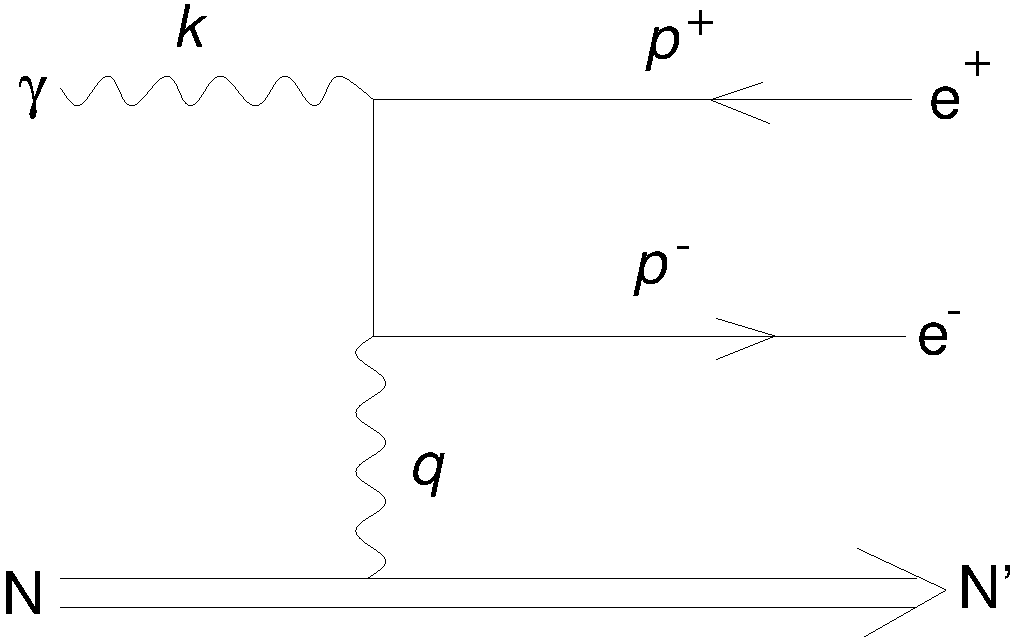
\includegraphics[height=8cm,width=12cm]{figures/pair}
\caption{\label{pair_fig} Feynman diagram for the pair
production process}
%\end{center}
\end{figure}
The triplet production process is similar but the interaction
takes place with one of the atomic electrons which receives
sufficient energy to be set free (so that there are 3 secondary electrons
produced in the interaction). By default
the triplet production process is
\index{triplet production}
not simulated explicitly but taken into account in an approximate
way by using the total pair+triplet cross section to
sample distances to subsequent pair production collisions.
By default EGSnrc adopts the cross sections used in EGS4, {\em i.e.}
%total cross sections taken from ??? and
extreme relativistic first Born approximation
(Coulomb corrected above 50 MeV)
differential cross sections  as formulated in the article by
Motz, Olsen and Koch \cite{Mo69}. For a photon energy
$k$ incident on the nucleus with the atomic number $Z$, the
differential pair production cross section is
\begin{eqnarray}
\label{pair-e}
& & {{\rm d}\sigma_{\rm pair}(Z,k,E_+) \over {\rm d}E_+}  =
{A_{\rm p}'(Z,k) r_0^2 \alpha Z (Z + \xi(Z) ) \over k}
\\ & & \quad
\left\{ \left( E_+^2 + E_-^2 \right) \left[ \phi_1(\delta) -
{4 \over 3} \ln Z  - 4 \tilde{f}_c(k,Z) \right] +
{2 \over 3} E_+ E_- \left[ \phi_2(\delta) -
{4 \over 3} \ln Z  - 4 \tilde{f}_c(k,Z) \right] \right\}
\nonumber
\end{eqnarray}
where $E_+$ and $E_-$ are the total energies of the
positron and electron,
\begin{equation}
\delta = 136 Z^{-1/3} 2 \Delta~,\quad \quad \Delta = {k m \over 2 E_+ E_-}
\end{equation}
and $\tilde{f}_c(Z)$ is the Coulomb correction,
\begin{equation}
\label{f_coulomb}
\tilde{f}_c(Z) =
\begin{cases}
f_c(Z), & k \ge 50~\text{MeV} \\
0, & \text{else}
\end{cases}
\end{equation}
where $f_c(Z)$ was derived by
Davies, Bethe and Maximon \cite{Da54},
\begin{equation}
\label{f_coulomb1}
f_c(Z) = a^2 \sum_{\nu=1}^\infty {1 \over \nu (\nu^2 + a^2)}, \quad
a = \alpha Z~.
\end{equation}
The empirical correction factor $A_{\rm p}'(k,Z)$ is
introduced in order to improve the total pair production
cross section at lower energies and is defined
as ``The best estimate of the total cross section
available divided by the total cross section resulting
from the integration of Eq. (\ref{pair-e}) with
$A_{\rm p}'(k,Z)=1$''. For energies above
50 MeV $A_{\rm p}'$ is taken to be unity, for
energies below 50 MeV the total pair+triplet cross sections compiled
by Storm and Israel \cite{SI70} are used.
The replacement $Z^2 \to Z (Z + \xi(Z))$ takes
into account the triplet production process, where $\xi(Z)$,
evaluated by the PEGS4 function {\tt XSIF},  is given by
\index{XSIF}
\begin{equation}
\xi(Z) = {L_{\rm rad}'(Z) \over L_{\rm rad}(Z) - f_c(Z)}
\end{equation}
where $f_c(Z)$ is defined in Eq. (\ref{f_coulomb}) and
$L,L'$ are Tsai's radiation logarithms \cite{Ts74},
\index{Tsai's radiation logarithms}
\begin{eqnarray}
L_{\rm rad}'(Z) & = &
\left\{
\begin{array}{r@{\quad , \quad}l}
\ln(1194\,Z^{-2/3}) &~~\mbox{if}~~~Z > 4 \\
6.144 & ~~\mbox{if}~~~Z = 1 \\
5.621 & ~~\mbox{if}~~~Z = 2 \\
5.805 & ~~\mbox{if}~~~Z = 3 \\
5.924 & ~~\mbox{if}~~~Z = 4
\end{array} \right. \nonumber \\
L_{\rm rad} & = &
\left\{
\begin{array}{r@{\quad , \quad}l}
\ln(184.15\,Z^{-1/3}) &~~\mbox{if}~~~Z > 4 \\
5.310 & ~~\mbox{if}~~~Z = 1 \\
4.790 & ~~\mbox{if}~~~Z = 2 \\
4.740 & ~~\mbox{if}~~~Z = 3 \\
4.710 & ~~\mbox{if}~~~Z = 4
\end{array} \right.
\end{eqnarray}
The functions $\phi_1(\delta)$ and $\phi_2(\delta)$, which
account for screening effects, are
given by
\begin{equation}
\begin{split}
\phi_1(\delta) & = 4 \int\limits_\Delta^1 {{\rm d}q \over q^3}
(q - \Delta)^2 \Big[1 - F(q,Z) \Big]^2 + 4 + {4 \over 3} \ln Z~,
\\
\phi_2(\delta) & = 4 \int\limits_\Delta^1  {{\rm d}q \over q^4}
\Big[q^3 - 6 \Delta^2 q \ln \left({q \over \Delta}\right) + 3 \Delta^2 q
-4 \Delta^3 \Big] \Big[1 - F(q,Z) \Big]^2 + {10 \over 3} + {4 \over 3} \ln Z
\end{split}
\end{equation}
where $q$ is the momentum transfer and $F(q,Z)$ the corresponding
atomic form factor for an atom with atomic
number $Z$. For a Thomas-Fermi potential $\phi_1(\delta)$
and $\phi_2(\delta)$ are independent of $Z$ and Butcher and
Messel have approximated them \cite{BM60} as
\begin{eqnarray}
\label{pair_phi}
\phi_1(\delta) & = & \left\{
\begin{array}{r@{\quad , \quad}l}
20.867 - 3.242 \delta + 0.625 \delta^2 & \delta \le 1 \\
21.12 - 4.184 \ln(\delta + 0.952) & \delta > 1
\end{array}
\right. \\
\phi_2(\delta) & = & \left\{
\begin{array}{r@{\quad , \quad}l}
20.029 - 1.93 \delta - 0.086 \delta^2 & \delta \le 1 \\
\phi_1(\delta) & \delta > 1
\end{array}
\right.
\end{eqnarray}

The differential pair production cross section for compounds
and mixture is derived from the independent atom approximation
and can be approximately written in the same form as Eq. (\ref{pair-e})
but replacing
\begin{eqnarray}
\label{pair_replace}
Z (Z + \xi(Z)) \quad & \mbox{with} & \quad Z_{\rm eff}^2 \equiv
\sum p_i Z_i (Z_i + \xi(Z_i) )
\nonumber \\
{1 \over 3} \ln Z + \tilde{f}_c(k,Z) \quad & \mbox{with} & \quad
Z_V \equiv \sum p_i
Z_i (Z_i + \xi(Z_i) ) \left[ {1 \over 3} \ln Z_i + \tilde{f}_c(k,Z_i) \right]
\nonumber \\
\delta \quad & \mbox{with} & \quad \delta_C 2 \Delta~,\quad
\delta_C \equiv {136 \over Z_{\rm eff}^2}
\sum p_i Z_i (Z_i + \xi(Z_i) ) Z_i^{-1/3}
\end{eqnarray}
where $p_i$ is the normalized fraction of atoms of type $i$ in
the molecule.

It is worth noticing that, due to the use of the extreme
relativistic approximation,  the differential cross
section as defined in Eq. (\ref{pair-e}) becomes inaccurate
for energies close to the threshold energy for pair production
(2 $\rm m$ ).
%and breaks down altogether for energies below
%2.1 MeV.
In the EGS4 implementation, the entire photon energy
was given to one of the pair particles for $k \le 2.1$ MeV.
We have defined a macro {\tt \$SELECT-LOW-ENERGY-PAIR-PRODUCTION}
which, in its default replacement, samples $E_+$ uniformly
in the allowed range $m \cdots k/2$. If the user is aware
of a better approach, this simplistic treatment can be
modified by the appropriate replacement of this macro.
\index{\$SELECT-LOW-ENERGY-PAIR-PRODUCTION}

\paragraph{NRC pair cross sections}\hfill
\index{pair cross sections!NRC}

In a more recent addition to EGSnrc, the user has the option
to specify use of a library of differential pair cross sections created
at the NRC. These cross sections are based on the exact partial-wave-analysis
calculations by {\O}verb{\o}, Mork and Olsen (OMO) \cite{Ov73} for the
unscreened nuclear potential modified by a multiplicative screening correction.
The main difficulty in creating this data library, which provides cross
sections up to 85 MeV for all elements between 1 and 100, consisted in finding
numerically stable approaches for performing the PWA summation for energies
above a few MeV (the OMO paper \cite{Ov73} only contains results up to 5.1 MeV).
Note that these cross sections take into account the asymmetry in the
positron-electron energy distribution and eliminate the need
for the {\tt \$SELECT-LOW-ENERGY-PAIR-PRODUCTION} macro mentioned
above.

In order to make use of the NRC pair cross sections, the user
\index{pair\_nrc}
must set the variable {\tt pair\_nrc}=1.  Note that
{\tt pair\_nrc} is part of the {\tt COMIN/BREMPR} common block
(see Section~\ref{common_blocks} of this report).

\paragraph{Explicit simulation of triplet production}\hfill
\index{triplet production}

In a more recent addition to EGSnrc, the user has the option
to explicitely simulate triplet production events according to the
first Born approximation result first derived by Votruba \cite{Vo48}
and later by Mork \cite{Mo67}. Due to the 3 particle final state the
expression for the differential triplet production cross section
is very complicated and so not reproduced here. It is worth
noting that the published expressions most likely contain typos
because their direct implementation in a computer program
lead to meaningless results ({\em e.g.} negative cross section within
the kinematically allowed range of energies and directions).
The triplet production cross section was therefore re-derived using
the CompHEP package, its results were manipulated using Mathematica and
were then output directly to Fortran code.

In order to turn on explicit simulation of triplet events, the user
\index{itriplet}
mist set the variable {\tt itriplet}=1. Note that
{\tt itriplet} is part of the {\tt COMIN/BREMPR} common block
(see Section~\ref{common_blocks} of this report).

The technique for sampling random directions and energies from
the differential triplet cross section is very involved.
Its detailed description awaits a future version of this report.


\paragraph{Simulation of pair production, particle energies}\hfill
\index{pair production!simulation of}

When the NRC pair differential cross section tabulations are used,
an alias table is employed for picking the positron energy.
For the default Bethe-Heitler cross sections,
the sampling algorithm implemented in EGS4 becomes extremely
inefficient as the incident photon energy approaches the
threshold energy. This is due to the following two facts:
(i) The electron and positron energies, $E_-$ and $E_+$,
are sampled in the range $0\cdots k/2$, the allowed
range becomes a small fraction of the above interval for
$k \to 2 m$. (ii) The rejection functions used are normalized
to their maximum at $\delta = 0$. For photon energies that
are not much larger than $2 m$ the actual possible maximum
is much smaller.

\index{EGS4}
We have therefore slightly modified the EGS4 pair production sampling algorithm to improve
its efficiency. If we define the functions
\begin{eqnarray}
B(\delta) & = & 3 \Big[ \phi_1(\delta) - 4 Z_V \Big] -
\Big[ \phi_2(\delta) - 4 Z_V \Big] \nonumber \\
C(\delta) & = & 3 \Big[ \phi_1(\delta) - 4 Z_V \Big] +
\Big[ \phi_2(\delta) - 4 Z_V \Big]
\end{eqnarray}
which will serve as rejection functions, and make
a change of variables,
\begin{equation}
\varepsilon  = {E_+ - m \over k - 2 m}~,
\end{equation}
the differential pair production cross section can be
rewritten as
\begin{equation}
{{\rm d} \sigma_{\rm pair} \over {\rm d} \varepsilon} =
N \left\{ {B(\delta) \over B_{\rm max}} + \left(1 - {2 m \over k} \right)^2
{A_{\rm max} \over 3 B_{\rm max}} A(\delta)
\left[ 12 \left(\varepsilon - \frac{1}{2} \right)^2 \right] \right\}
\end{equation}
where $N$ combines all constant factors that are irrelevant for
the sampling algorithm and $A_{\rm max}$ and $B_{\rm max}$ are
the maxima of the rejection functions $A(\delta)$ and $B(\delta)$,
\begin{equation}
A_{\rm max} = A\left({4 \delta_C m \over k}\right)~, \quad \quad
B_{\rm max} = B\left({4 \delta_C m \over k}\right)~.
\end{equation}
The sampling algorithm, which determines the energy
of the lower energy ``electron'' is then as follows:
\begin{enumerate}
\item
Calculate $A_{\rm max}$, $B_{\rm max}$ and $\alpha$,
\begin{equation}
\alpha = {1 \over 1 + (1 - 2 m/k)^2 A_{\rm max}/3/B_{\rm max}}
\end{equation}
To save time at high energies, use $A_{\rm max} = A(0)$ and
$B_{\rm max} = B(0)$ for $k \ge 50$~MeV.
\item
Draw a random number $r_1$
\item
If $r_1 > \alpha$, then sample $\varepsilon$
from $12 (\varepsilon - 1/2 )^2$, {\em i.e.}
\begin{equation}
\varepsilon = \frac{1}{2} \left(1 - \mbox{Max}\{r_2,r_3,r_4\}\right)
\end{equation}
and use $A(\delta)/A_{\rm max}$ as a rejection function in step 5
\item
Else, sample $\varepsilon$ uniformly, {\em i.e.}
\begin{equation}
\varepsilon = \frac{1}{2} r_2
\end{equation}
and use $B(\delta)/B_{\rm max}$ as a rejection function in step 5
\item
Calculate $\delta$ and the rejection function $R$ = $A(\delta)/A_{\rm max}$ or
$B(\delta)/B_{\rm max}$
\item
If $r_5 < R$, accept $\varepsilon$, else go to step 2.
\end{enumerate}

\begin{figure}[h]
%\setlength{\vsize}{12cm}
%\setlength{\abovecaptionskip}{0.5in}
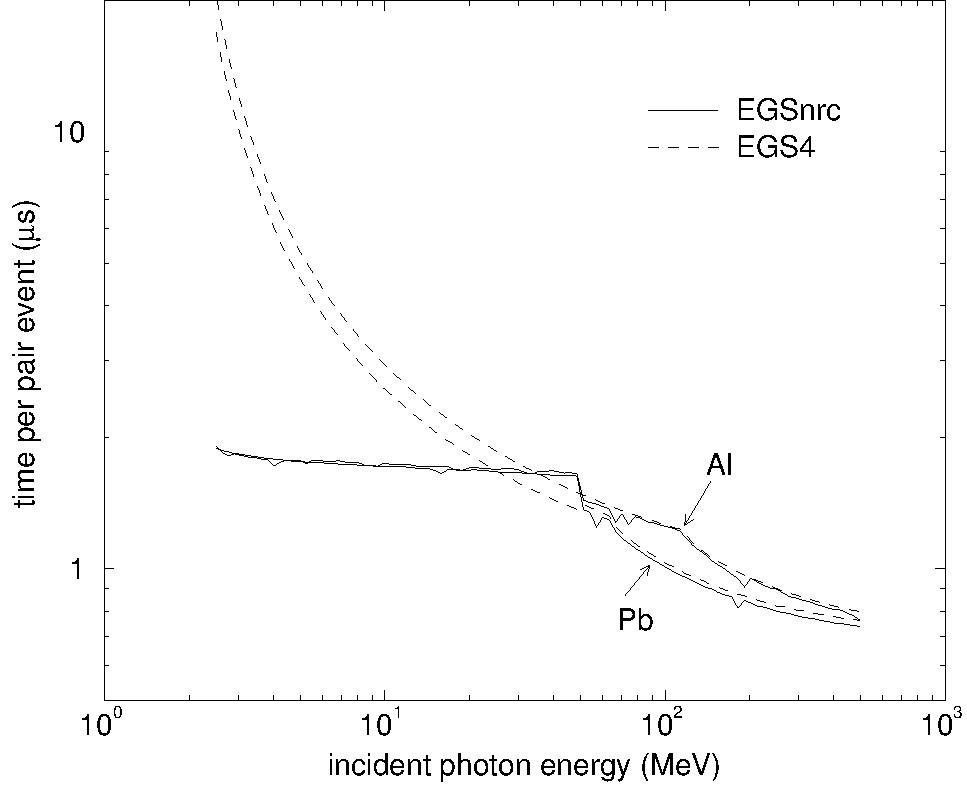
\includegraphics[height=12cm,width=12cm]{figures/pair_times}
\caption[CPU time for pair sampling]{\label{pair_times}
CPU time in $\mu$s on a 500 MHz PIII computer to sample a pair energy.}
\end{figure}

Fig. \ref{pair_times} shows the CPU time in $\mu$s on a 500 MHz PIII computer
running Linux necessary to sample a pair energy using the
algorithms discussed here (solid lines) and the original EGS4
algorithm (dashed lines) for aluminum and lead as a function
of the incident photon energy (this is just the time for
energy sampling, excluding angle sampling and rotations). Note
the logarithmic scale and the dramatic increase in CPU time for
the EGS4 algorithm and a photon energy less then 20 or 30 MeV.
The discontinuity in the EGSnrc algorithm around $50$~MeV
is due change in the
approach to calculate $A_{\rm max}$ and $B_{\rm max}$  (see item 1).

\paragraph{Simulation of pair production, particle angles}\hfill
\index{pair production!angular distribution}

\index{Bielajew, Alex} \index{EGS4}
In the original EGS4 version electrons and positrons were
produced at a fixed polar angle $\theta_{\pm}$ with respect to the direction
of the incoming photon given by $\theta_{\pm}=m/k$. This approach
was subsequently improved as discussed in PIRS Report 0287
\cite{Bi91} which introduced the {\tt \$SET-PAIR-ANGLE} macro
as an NRC extension to the EGS4 system.
This macro is now included in the EGSnrc system. The angle
selection procedure is controlled by the variable
{\tt IPRDST} (part of the {\tt COMIN/EDGE} common block--
see Section~\ref{common_blocks}) which can assume the following values:
\index{IPRDST}
\begin{itemize}
\item[]{\tt IPRDST=0}: The original EGS4 approach is used,
{\em i.e.} $\theta_{\pm}=m/k$
\item[]{\tt IPRDST=1}: The leading order term of the angular distribution
is employed, {\em i.e.}
\begin{equation}
\label{pair_ang1}
{{\rm d} \sigma \over {\rm d} \Omega_\pm} = N
{1 \over (1 - \beta_\pm \cos \theta_\pm)^2}
\end{equation}
where $N$ is again a normalization constant and $\beta_\pm$ denotes
the velocity of the positron or electron in units of the speed of light.
\item[]{\tt IPRDST=2}: The formula 3D-2003 of the article by
Motz {\em et al.} \cite{Mo69} is used, which is the cross section, differential
\index{IPRDST}
in electron/positron energy and angle:
\end{itemize}
\begin{equation}
\label{pair_ang_2}
\begin{split}
{{\rm d} \sigma \over {\rm d} E_\pm {\rm d} \Omega_\pm} & =
{N \over (u^2+1)^2 }
\left\{ -(E_+ - E_-)^2 - {16 u^2 E_+ E_- \over (u^2 + 1)^2} +
\left[ E_+^2 + E_-^2 + {4 u^2 E_+ E_- \over (u^2 + 1)^2} \right]
\ln M(k,E_\pm,u) \right\} \\
u & =  E_\pm \theta_\pm~, \quad {1 \over M(k,E_\pm,u)} =
\left({k \over 2 E_+ E_-} \right)^2 + \left( { Z_{\rm eff}^{1/3} \over
111 (u^2 + 1)^2 } \right)^2
\end{split}
\end{equation}
\begin{itemize}
\item[\phantom{\tt IPRDST=2}]
where all energies are measured in units of $m$.
Note that Eq. (\ref{pair_ang_2}) is based on an extreme relativistic,
small angle approximation where
\begin{equation}
\begin{split}
(1 - \beta_\pm \cos \theta_\pm)^2 & \approx
\left[1 - \beta_\pm \left(1 - \frac{\theta_\pm^2}{2}\right) \right]^2
= (1 - \beta_\pm)^2 \left[ 1 - {\beta_\pm \over 1 - \beta_\pm}
\frac{\theta_\pm^2}{2} \right]^2 \\
& \approx  (1 - \beta_\pm)^2 (1 + u^2)^2~.
\end{split}
\end{equation}
Perhaps, it would be a good idea to replace $1+u^2$ with
$1 - \beta_\pm \cos \theta_\pm$ in the denominator outside
of the curled brackets of Eq. (\ref{pair_ang_2}), but
we have not undertaken this modification.
\end{itemize}

The sampling algorithm for Eq. (\ref{pair_ang_2}) is discussed
extensively in Ref. \cite{Bi91}.
\index{Bielajew, Alex}
%.
It should be noted that
this algorithm becomes progressively more inefficient with
increasing energies. Given this fact and the approximations
involved which make its use questionable at low energies,
we have chosen {\tt IPRDST=1} as the default
pair angle selection scheme in EGSnrc. The generation
of electron and positron polar angles from the
distribution (\ref{pair_ang1}) is trivial, it
is accomplished by
\index{IPRDST}
\begin{equation}
\cos \theta_\pm = {2 r - 1 + \beta_\pm \over \beta_\pm (2 r -1 ) + 1}
\end{equation}
where $r$ is an uniformly distributed random number between zero and
unity. As pair-production is a three-body process, separate polar
angles for the electron and positron are needed. The two
azimuthal angles are chosen to be opposite. This is,
strictly speaking, not correct, but due to lack of a better
alternative, adopted from the original EGS4 version.

\paragraph{Russian Roulette for pair production events} \hfill
\index{Russian Roulette}
\index{variance reduction!Russian Roulette}
\index{pair production!Russian Roulette}

It is wasteful to simulate all pair production events if
the user intends to play Russian Roulette with electrons
set in motion in photon interactions. We have therefore implemented
an EGSnrc internal Russian Roulette scheme which is turned on
by setting the flag {\tt i\_play\_RR} which is in {\tt
COMIN/EGS-VARIANCE-REDUCTION/}
to 1. The survival probability for the electrons is
{\tt prob\_RR}, also in {\tt COMIN/EGS-VARIANCE-REDUCTION/}.
If {\tt i\_play\_RR} is set, the following actions are
taken at the beginning of subroutine {\tt PAIR}:
\index{EGS-VARIANCE-REDUCTION}
\index{prob\_RR} \index{i\_play\_RR}
\begin{enumerate}
\item
Pick a random number $r$
\item
If $r > $~{\tt prob\_RR}, reduce the stack size by one, return
to {\tt PHOTON} ({\em i.e.} save the simulation of the pair event).
If the stack becomes empty, a zero weight, zero energy photon
is left on the stack so that the {\tt PHOTON} routine can exit
properly.
\item
If $r < $~{\tt prob\_RR}, increase the weight of the current photon by
1/prob\_RR and simulate the pair event as usual.
\end{enumerate}
For more discussion of Russian Roulette see sections~\ref{rusrou} and
\ref{step_5b}.

\subsubsection{Incoherent (Compton) scattering}
\setcounter{equation}{0}
\label{compton}
\index{bound Compton scattering}
\index{Compton scattering}
\index{incoherent scattering}
\index{cross section!incoherent}

\paragraph{Cross section}\hfill

The Feynman diagram for the Compton scattering process is
shown in Fig. \ref{compt_fig}. The circle in the line
of the incoming atom A indicates that the electron
\begin{figure}[h]
%\begin{center}
%\setlength{\hsize}{15cm}
%\setlength{\vsize}{8cm}
%\setlength{\abovecaptionskip}{0.5in}
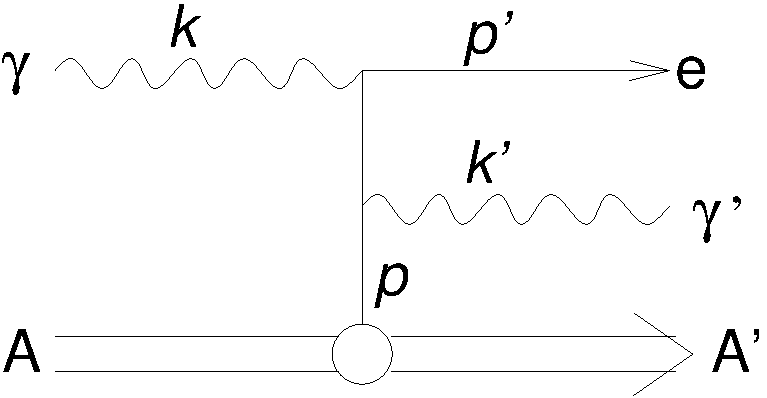
\includegraphics[height=8cm,width=12cm]{figures/compt}
\caption{\label{compt_fig} Feynman diagram for the Compton process}
%\end{center}
\end{figure}
is initially bound to the atom and represents the probability
that an atomic electron with a four-momentum $p = (E,\vec{p})$
interacts with the incoming photon with a four-momentum
$k=(k,\vec{k})$ into a final $e^-\gamma'$ state given by
$k'=(k',\vec{k'})$ and $p'=(E',\vec{p}')$.
To simplify the notation, all energies will be measured
in units of the electron's rest energy $m$ and all momenta
in units of $m/c$ in the following equations of this
section.

\index{Klein-Nishina}
If the binding to the atom is neglected and the electron
is considered to be initially at rest ({\em i.e} $p = (1,0,0,0)$),
the cross section for the process is given by the Klein-Nishina
formula \cite{KN29},
\begin{equation}
{{\rm d} \sigma_{\rm KN} \over {\rm d} \cos \theta} = \pi r_0^2 Z~
X_{\rm KN}~, \quad \quad X_{\rm KN} =
\left({k_c \over k} \right)^2
\left[ {k_c \over k} + {k \over k_c} - \sin^2 \theta \right]
\end{equation}
where $\theta$ is the polar angle of the scattered photon with
respect to the initial direction and $k_c$ is the energy
of a photon scattered at an angle $\theta$
by free electrons at rest,
\begin{equation}
k_c = {k \over 1 + k (1 - \cos \theta)}
\end{equation}
\index{Doppler broadening}
\index{incoherent scattering!binding effects}
\index{incoherent scattering!Doppler broadening}
The treatment of the Compton process in EGS4 is based on these
equations with $k' = k_c$. In EGSnrc we have included binding effects and
Doppler broadening according to the impulse approximation (IA)
\cite{Ri75}. The IA assumes that the potential in which the
target electrons move is constant so that their states can
be represented by plane waves. The double differential
cross section for photon scattering into the final state
$k' = (k', k' \sin \theta \cos \phi, k' \sin \theta \sin \phi, \\
k' \cos \theta)$ is given by (Eq. (15) of Ref. \cite{RB82})
\begin{equation}
\label{comp_cs1}
{{\rm d}^2 \sigma_{\rm comp} \over {\rm d}k' {\rm d}\Omega} =
{r_0^2 \over 2} {k' \over k q} \Big[1 + p_z^2 \Big]^{-1/2} X J(p_z)
\end{equation}
where $\Omega$ is the solid angle $(\theta,\phi)$ and where
\begin{itemize}
\item
$q$ is the modulus of the momentum transfer vector
$\vec{q} = \vec{k'} - \vec{k}$,
\begin{equation}
q = \sqrt{k^2 + k^{\prime 2} - 2 k k' \cos \theta}
\end{equation}
\item
$p_z$ is the projection of the initial electron momentum
on the direction of $\vec{q}$,
\begin{equation}
\label{comp_pz}
p_z = {\vec{p} \cdot \vec{q} \over q} =
{k k' (1 - \cos \theta) - k + k' \over q}
\end{equation}
Note that the above equation is derived from a non-relativistic
approximation and requires $|p_z| \le 1$.
\item
$X$ is defined as
\begin{eqnarray}
X & = & {R \over R'} + {R' \over R} +
2 \left(\frac{1}{R} - \frac{1}{R'} \right)
+ \left(\frac{1}{R} - \frac{1}{R'} \right)^2 \nonumber \\
R & = & k \left[ \sqrt{1 + p_z^2} + {k - k' \cos \theta \over q} p_z \right]
\nonumber \\
R' & = & R - k k' (1 - \cos \theta)~.
\end{eqnarray}
Note that $R$ and $R'$ simplify to
\begin{equation}
R \approx k \left(1 + O(p_z) \right)~, \quad
R' \approx k \Big[1 - k_c (1 - \cos \theta ) \Big] \left(1 + O(p_z) \right)
\end{equation}
for $p_z \ll 1$. In this limit
\begin{equation}
X = X_{\rm KN} \left(1 + O(p_z) \right)
\end{equation}
\item
The function $J(p_z)$ is the Compton profile,
\begin{equation}
J(p_z) = \int {\rm d} p_x {\rm d} p_y | \psi(\vec{p}) |^2~,
\end{equation}
where $\psi(\vec{p})$ is the wave function of the bound electrons.
Extensive tables of atomic and shell-wise
\index{Compton profiles}
\index{incoherent scattering!Compton profiles}
Hartree-Fock Compton profiles for all
elements have been published by Biggs {\em et al} \cite{BM75}.
Following Brusa {\em et al} \cite{BS96},
contributions
from different electron shells are considered separately, so
that the atomic or molecular Compton profile is the sum
of one-electron shell Compton profiles $J_i(p_z)$, and binding effects
are taken into account by rejecting interactions that
transfer less energy to the electron than the binding energy $U_i$,
{\em i.e.}
\begin{equation}
J(p_z) = \sum Z_i J_i(p_z) \Theta(k - k' - U_i)~.
\end{equation}
Here, $Z_i$ is the occupation number of shell $i$ and
the $J_i$ have the normalization
\begin{equation}
\int\limits_{-\infty}^\infty {\rm d} p_z J_i(p_z) = 1
\end{equation}
\end{itemize}
With all this, and after changing the cross section
from differential in $k'$ to differential in $p_z$,
Eq. (\ref{comp_cs1}) can be written as
\begin{equation}
{{\rm d}^2 \sigma_{\rm comp} \over {\rm d}p_z {\rm d}\Omega} =
{r_0^2 \over 2} X_{\rm KN}
\left( \sum Z_i J_i(p_z) \Theta(k - k' - U_i) \right) F(k,\cos \theta, p_z)
\end{equation}
where the function $F(k,\cos \theta, p_z)$ combines all remaining
factors times ${\rm d}k'/{\rm d}p_z$,
\begin{equation}
F(k,\cos \theta, p_z) = \frac{k'}{k_c} \Big[ 1 + p_z^2 \Big]^{-1/2}
\frac{X}{X_{\rm KN}} \left(1 + \frac{k_c}{k} {k \cos \theta - k' \over q} p_z
\right)^{-1}
\end{equation}
Here, $k'$ is a function of $k, \cos \theta$ and $p_z$ and
follows from solving Eq. (\ref{comp_pz}) with respect to $k'$,
{\em i.e.}
\begin{equation}
\label{comp_kprime}
k' = {k_c \over 1 - p_z^2 \varepsilon^2 } \left[
1 - p_z^2 \varepsilon \cos \theta + p_z \sqrt{1 - 2 \varepsilon
\cos \theta + \varepsilon^2 \left(1 - p_z^2 \sin^2 \theta \right) }~ \right]~,
\quad \quad \varepsilon = \frac{k_c}{k}
\end{equation}
The incoherent scattering cross section, differential in
the photon scattering angle, is
\begin{equation}
\label{comp_sig_omega}
{{\rm d} \sigma_{\rm comp} \over {\rm d}\Omega} =
{r_0^2 \over 2}
%\left(\frac{k_c}{k} \right)^2 : must not be there, noted by Trent Hawkins
X_{\rm KN} S(k,\cos \theta)
\end{equation}
where
\begin{equation}
\label{comp_sincoh}
S(k,\cos \theta) =
\sum Z_i \Theta(k - U_i) S_i, \quad \quad
S_i = \int\limits_{-\infty}^{p_i} {\rm d} p_z J_i(p_z)
F(k,\cos \theta, p_z)
\end{equation}
\index{incoherent scattering function}
can be identified with the incoherent scattering function.
The upper limit of the $p_z$ integration for the $i$'th shell, $p_i$,
\begin{equation}
\label{comp_pi}
p_i = { k (k - U_i) (1 - \cos \theta) - U_i \over
\sqrt{ 2 k (k - U_i) (1 - \cos \theta) + U_i^2}}~,
\end{equation}
follows from Eq. (\ref{comp_pz}) with
$k' = k - U_i$ and assures that sufficient energy is transferred
to the electron to set it free. To first order, $S(k,\cos \theta)$
depends only on $k \sqrt{(1 - \cos \theta)/2}$ and so,
Namito {\em et al} \cite{Na94} use tabulated
incoherent scattering functions in their
extension of the EGS4 system to include binding effects
and Doppler broadening, when sampling the photon scattering angle.
This approach introduces a slight inconsistency in their treatment
of the Compton process.

As the Compton profiles are
strongly peaked around $p_z=0$, the main contributions
to the integral come from small $p_z$ values where
the function $F(k,\cos \theta, p_z)$ is very close
to unity and so, Brusa {\em et al} \cite{BS96} approximate
$S(k,\cos \theta)$ with
\begin{equation}
\label{comp_sincoh1}
S(k,\cos \theta) \approx S_A((k,\cos \theta) \equiv
\sum Z_i \int\limits_{-\infty}^{p_i} {\rm d} p_z J_i(p_z)
\Theta(k - U_i)
\end{equation}
for their implementation of binding effects and Doppler broadening
in the PENELOPE system \cite{Sa96}\footnote{They take
into account $F(k,\cos \theta, p_z)$, using its Taylor
expansion up to $O(p_z)$, for the sampling of $p_z$.}
\begin{figure}[h]
%\begin{center}
%\setlength{\vsize}{12cm}
%\setlength{\abovecaptionskip}{0.5in}
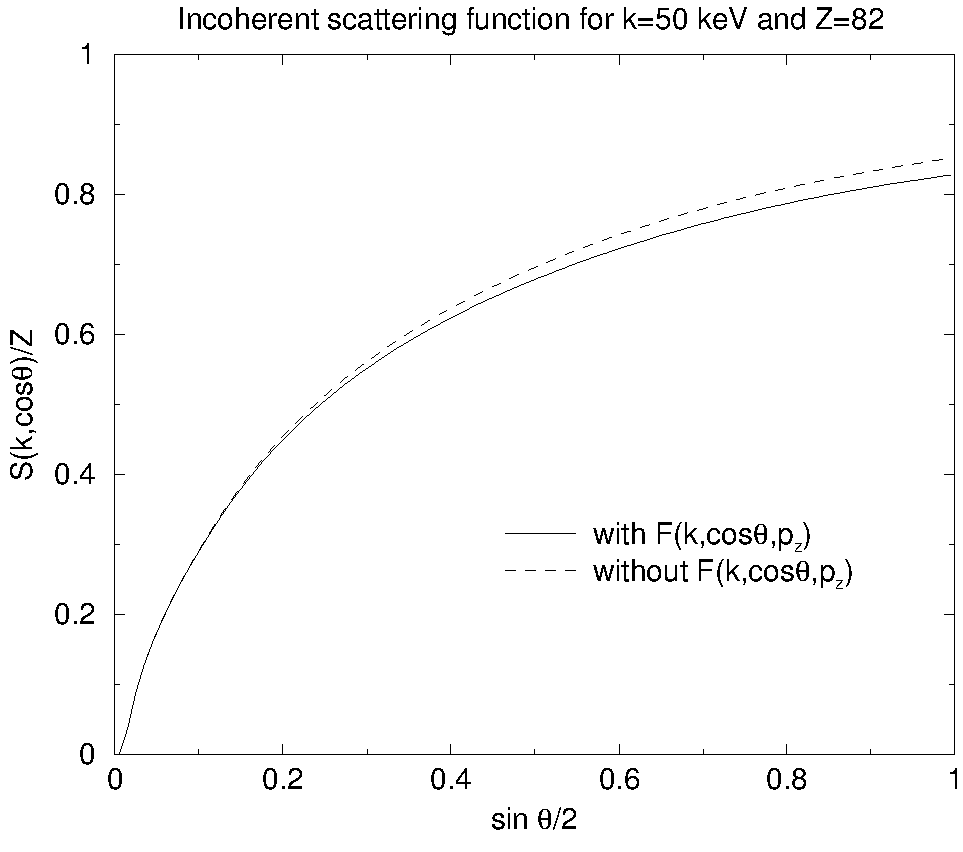
\includegraphics[height=12cm,width=12cm]{figures/sincoh}
%\end{center}
\caption[Incoherent scattering function]{\label{comp_sincoh_fig}
The incoherent scattering function for lead and $k=50$~keV
calculated from Eq. (\protect\ref{comp_sincoh}) (solid line)
and from Eq. (\protect\ref{comp_sincoh1}) (dashed line)
by numerical integration}.
\end{figure}
This approach introduces a small error at low energies
for high $Z$ materials as can be seen
in Fig. \ref{comp_sincoh_fig} which shows
$S(k,\cos \theta)$ for 50 keV photons in lead calculated
with or without taking into account $F(k,\cos \theta, p_z)$.

To minimize the amount of data necessary for
the simulation of the Compton process, and to make
the calculation of the incoherent scattering function ``on the fly''
possible, we use
the analytical approximations for the Compton profiles
$J_i(p_z)$ proposed by Brusa {\em et al} \cite{BS96}:
\begin{equation}
\label{comp_Japprox}
J_i(p_z) = J_{i,0} (1 + 2 J_{i,0} |p_z| ) \exp\left[\frac{1}{2} -
\frac{1}{2}\left(1 + 2 J_{i,0} |p_z| \right)^2\right]
\end{equation}
where $J_{i,0} \equiv J_i(0)$ is the value of the profile at
$p_z = 0$ obtained from the Hartree-Fock orbital \cite{BM75}.
In addition, we approximate $F(k,\cos \theta, p_z)$ by
\begin{equation}
\label{comp_Fapprox}
F((k,\cos \theta, p_z) = \left\{
\begin{array}{l@{\quad , \quad}l}
1 - \alpha p & p_z \le -p \\
1 + \alpha p_z & |p_z| < p \\
1 + \alpha p & p_z \ge p
\end{array} \right.
\end{equation}
where
\begin{eqnarray}
\label{comp_alpha}
\alpha & = & \frac{q_c}{k} \left(1 +
{k_c (k_c - k \cos \theta) \over q_c^2} \right)
\nonumber \\
q_c & = & \sqrt{k^2 + k_c^2 - 2 k k_c \cos \theta}~.
\end{eqnarray}
Equation (\ref{comp_Fapprox}) results from a Taylor series
expansion of $F(k,\cos \theta, p_z)$ up to $O(p_z)$. As this
approximation becomes inaccurate for large $p_z$ values
it is applied only for $|p_z| < p$, else the function values at
$\pm p$ are used. We have checked by numerical integration
of Eq. (\ref{comp_sincoh}) that the incoherent scattering function
calculated with the approximation (\ref{comp_Fapprox}) agrees
to better than 0.3\% with the incoherent scattering function
calculated using the exact expression for $F(k,\cos \theta, p_z)$
if $p = 0.15$ is used.

Combining now Eq. (\ref{comp_sincoh}), (\ref{comp_Japprox}) and
(\ref{comp_Fapprox}),  we obtain for $S_i$
%\begin{equation}
%S_i(k,\cos \theta) = \left\{
%\begin{array}{l@{\quad , \quad}l}
%(1 - \alpha p) {e^{-b} \over 2} & p_z \le -p \\
%(1 + \alpha p_z) {e^{-b} \over 2} - {\alpha \over 4 J_{i,0}}
%\sqrt{{\pi \over 2}} e^{1/2} \left[ \mbox{Erf} \left( 1 + 2 J_{i,0} p \over
%\sqrt{2} \right) - \mbox{Erf} \left(  1 + 2 J_{i,0} |p_z|
%\over \sqrt{2} \right) \right] & -p < p_z \le 0  \\
%1 - (1 + \alpha p_z) {e^{-b} \over 2} - {\alpha \over 4 J_{i,0}}
%\sqrt{{\pi \over 2}} e^{1/2} \left[ \mbox{Erf} \left( 1 + 2 J_{i,0} p \over
%\sqrt{2} \right) - \mbox{Erf} \left(  1 + 2 J_{i,0} |p_z|
%\over \sqrt{2} \right) \right] & 0 < p_z < p \\
%1 - (1 + \alpha p) {e^{-b} \over 2} & p_z \ge p
%\end{array} \right.
%\end{equation}
\begin{eqnarray}
\label{comp_Si}
& & S_i(k,\cos \theta) \nonumber \\
& = & (1 - \alpha p) {e^{-b} \over 2}~,\quad \mbox{if}~~p_i \le -p \nonumber \\
& = &
(1 + \alpha p_i) {e^{-b} \over 2} - {\alpha \over 4 J_{i,0}}
\sqrt{{\pi \over 2}} e^{1/2} \left[ \mbox{Erf} \left( 1 + 2 J_{i,0} p \over
\sqrt{2} \right) - \mbox{Erf} \left(  1 + 2 J_{i,0} |p_i|
\over \sqrt{2} \right) \right]~,\quad \mbox{else if}~~ p_i \le 0 \nonumber \\
& = &
1 - (1 + \alpha p_i) {e^{-b} \over 2} - {\alpha \over 4 J_{i,0}}
\sqrt{{\pi \over 2}} e^{1/2} \left[ \mbox{Erf} \left( 1 + 2 J_{i,0} p \over
\sqrt{2} \right) - \mbox{Erf} \left(  1 + 2 J_{i,0} |p_i|
\over \sqrt{2} \right) \right] ~,\quad \mbox{else if}~~ p_i < p \nonumber \\
& = &
1 - (1 + \alpha p) {e^{-b} \over 2} ~,\quad \mbox{else}
\end{eqnarray}
where
\begin{equation}
b = \frac{1}{2}\left(1 + 2 J_{i,0} |p_i| \right)^2 - \frac{1}{2}
\end{equation}
and $\mbox{Erf}$ is the error function. It is worth noticing that
$S_i$ is always less or equal to unity. This fact allows for
using it as a rejection function in the sampling algorithm discussed
in the next section.

The total incoherent scattering cross section $\sigma_{\rm comp}^{\rm (tot)}$
can be obtained
by a numerical integration over all scattering angles from
Eq. (\ref{comp_sig_omega}), (\ref{comp_sincoh}) and
(\ref{comp_Si}). To
avoid substantial changes of the data preparation program PEGS4,
we use instead the total Klein-Nishina cross section,
$\sigma_{\rm KN}^{\rm (tot)}$, while tracking the photons through
the geometry, and reject Compton interactions with the probability
$1-\sigma_{\rm comp}^{\rm (tot)}/\sigma_{\rm KN}^{\rm (tot)}$ once
at the interaction site (fictitious cross section method).
This rejection probability results automatically (without
calculating $\sigma_{\rm comp}^{\rm (tot)}$) from the sampling
algorithm, as we shall see in the next section.

\index{IBCMP}
Another advantage of this approach is that the user can
turn on or off binding effects and Doppler broadening
using the switch {\tt IBCMP} (included in the common
block {\tt COMIN/COMPTON-DATA}--see Section~\ref{common_blocks}),
without preparing two
separate material data files. The only additional data
needed to simulate incoherent scattering in the impulse
approximation are the Compton profile parameters
$J_{i,0}$, taken from the tabulations by Biggs {\em et al}
\cite{BM75}, and the occupation numbers $Z_i$ and
binding energies $U_i$ for all elements, taken from
Lederer and Shirley \cite{LS78}. These data are read in
in subroutine {\tt init\_compton} which is called from
{\tt HATCH}.
\index{init\_compton}

\paragraph{Simulation of incoherent scattering events}\hfill
\index{incoherent scattering!simulation of}
\index{Compton scattering!simulation of}
\index{bound Compton scattering}

The incoherent scattering cross section, differential in
the photon scattering angle $\Omega = (\theta,\phi)$
and the Doppler broadening
parameter $p_z$, per interaction site sampled from the
total Klein-Nishina cross section is
\begin{eqnarray}
{{\rm d}^2 \sigma_{\rm comp} \over \sigma_{\rm KN}^{\rm (tot)}} & = &
\sum \frac{Z_i}{Z} \Theta(k - U_i)~ \sigma_i~ {\rm d} \Omega~ {\rm d} p_z
\\
\sigma_i~ {\rm d} \Omega~ {\rm d} p_z & = &
%\left( \int\limits_{-\infty}^{p_i} {\rm d} p_z J_i(p_z) F(k,\cos \theta,p_z)
%\right)~
S_i~
{{\rm d} \phi \over 2 \pi}~
{X_{\rm KN}(\cos \theta)~{\rm d} \cos \theta~ \over
\int\limits_{-1}^1 X_{\rm KN}(\cos \theta) {\rm d} \cos \theta }
~{ J_i(p_z) F(k,\cos \theta,p_z) \Theta(p_i - p_z) {\rm d} p_z \over
\int\limits_{-\infty}^{p_i} {\rm d} p_z J_i(p_z) F(k,\cos \theta,p_z) }
\nonumber
\end{eqnarray}
It is then clear that the following algorithm produces the
required number of rejections and samples the differential
cross section correctly, if the interaction is accepted:
\begin{enumerate}
\item
Sample the shell number $i$ using the probabilities $Z_i/Z$
\item
If the incident photon energy $k$ is smaller than the binding
energy $U_i$, reject the interaction,
else, sample $\cos \theta, \phi$ and $p_z$ using the differential
cross section $\sigma_i$ of the selected shell as follows:
\item
Sample the photon polar scattering angle $\theta$ using
\begin{displaymath}
P_1(\cos \theta) =
{X_{\rm KN}(\cos \theta)~{\rm d} \cos \theta~ \over
\int\limits_{-1}^1 X_{\rm KN}(\cos \theta) {\rm d} \cos \theta }
\end{displaymath}
which is a normalized probability distribution function (PDF). The method
for sampling $\cos \theta$ will be explained below.
\item
Calculate the maximum possible value of $p_z$, $p_i$, from
Eq. (\ref{comp_pi}), and $S_i$ from Eq. (\ref{comp_Si}).
\item
If a uniformly distributed random number is greater then $S_i$,
reject the interaction
\item
Sample $p_z$ from
\begin{displaymath}
P_2(p_z) =
{ J_i(p_z) F(k,\cos \theta,p_z) \Theta(p_i - p_z) {\rm d} p_z \over
\int\limits_{-\infty}^{p_i} {\rm d} p_z J_i(p_z) F(k,\cos \theta,p_z) }
\end{displaymath}
which is a normalized PDF for $p_z$. The sampling
technique employed for this distribution function is explained below.
\item
Sample the azimuthal scattering angle from ${\rm d}\phi/(2 \pi)$
\item
Calculate the energy $k'$ of the scattered photon from
Eq. (\ref{comp_kprime})
\item
The electron set in motion has then a kinetic energy of $k - k' - U_i$,
a polar scattering angle $\theta_e$ given by
\begin{equation}
\cos \theta_e = {k - k' \cos \theta \over
\sqrt{k^2 + k^{\prime 2} - 2 k k' \cos \theta} }
\end{equation}
and an azimuth opposite to the photon's azimuth.
\end{enumerate}
Note that if the user does not want to take into account binding
effects and Doppler broadening (the switch {\tt IBCMP} is set to zero)
the sampling algorithm consists of steps 3, 7 and 9 with
$k' = k_c$ and $U_i = 0$.
\index{IBCMP}

As the shell with which the interaction takes place is explicitly determined
in step 1, at the end of the sampling algorithm the vacancy created
by the Compton process is known. The relaxation of shell vacancies
\index{relaxations}
\index{atomic relaxations}
with binding energies above the specified transport threshold
energies is performed in subroutine {\tt relax} (see section \ref{relax}) and
may lead to the creation of additional fluorescent photons and
Auger and Coster-Kronig electrons on the stack. Many of the
EGS4 based user codes assume that the outcome of an incoherent scattering
process is a scattered photon and a Compton electron. This assumption
is obviously not satisfied for EGSnrc, the outcome of an incoherent
event may by any one of the following:
\begin{enumerate}
\item
The original photon, if the interaction was rejected due to the one
of the rejection criteria
\item
A scattered photon and a Compton electron, if all relaxation particles
had energies below the specified transport threshold energies
({\tt ECUT} and {\tt PCUT})
\item
A scattered photon, a Compton electron plus $n$ relaxation particles, else.
\end{enumerate}
See section~\ref{stack_status} (page~\pageref{stack_status}) for more
information.

Finally, the portion of the binding energy that resulted in the creation
of sub-threshold relaxation particles is made known to the user via
a call to the scoring routine {\tt AUSGAB} with the argument {\tt IARG=4}.
\index{AUSGAB}
\index{IARG!4}

We conclude this section with some details about steps 3, 4 and 6
of the sampling algorithm.

\underline{Step 3, sampling of $\cos \theta$}: Following
the EGS4 manual\cite{Ne85} we rewrite
the PDF $P_1$ in terms of $\varepsilon = k_c/k$,
\index{SLAC-265}
\begin{equation}
\label{comp_P1}
P_1(\varepsilon) = P_1(\cos \theta) {{\rm d}\varepsilon \over
{\rm d} \cos \theta} = N \left( \frac{1}{\varepsilon} + \varepsilon -
\sin^2 \theta \right)
\end{equation}
where $N$ is a normalization constant that is irrelevant for the sampling
algorithm. The minimum and maximum possible values for
$\varepsilon$, $\varepsilon_{\rm min}$ and $\varepsilon_{\rm max}$, follow
from $\cos \theta = -1$ and $\cos \theta = 1$, respectively, and are
given by
\begin{equation}
\varepsilon_{{\rm min}} = {1 \over 1 + 2 k}~, \quad \quad
\varepsilon_{{\rm max}} = 1~.
\end{equation}
Equation (\ref{comp_P1}) can be further rewritten as
\begin{equation}
P_1(\varepsilon) = N (\alpha_1 + \alpha_2) \left\{
{\alpha_1 \over \alpha_1 + \alpha_2}~
\left({1 \over \varepsilon \alpha_1} \right)
+ {\alpha_2 \over \alpha_1 + \alpha_2}~\left({ \varepsilon \over \alpha_2}
\right) \right\} \left[ 1 - {\varepsilon \sin^2 \theta \over 1 +
\varepsilon^2 } \right]
\end{equation}
with
\begin{equation}
\alpha_1  =  \ln \left(1 + 2 k \right)~, \quad \quad
\alpha_2  = {1 - \varepsilon_{\rm min}^2 \over 2}
\end{equation}
$1/\varepsilon/\alpha_1$ and $\varepsilon/\alpha_2$ are
normalized PDFs, they can be used to sample $\varepsilon$
with the probability $\alpha_1/(\alpha_1 + \alpha_2)$ and
$\alpha_2/(\alpha_1 + \alpha_2)$, respectively. The expression
of the square brackets has a maximum of unity for
$\varepsilon = 1$ ($\sin \theta = 0$) and is thus
a valid rejection function. The sampling algorithm is then as follows:
\begin{itemize}
\item[3.1]
Calculate $\varepsilon_{\rm min}, \alpha_1, \alpha_2$ and
$w = \alpha_1/(\alpha_1 + \alpha_2)$
\item[3.2]
Pick three random numbers $r_1, r_2$ and $r_3$
\item[3.3]
If $r_1 \le w$,
\begin{equation}
\varepsilon = \varepsilon_{\rm min} \exp( r_2 \alpha_1 )~,
\end{equation}
else,
\begin{equation}
\varepsilon = \sqrt{ \varepsilon_{\rm min}^2 + 2 r_2 \alpha_2}
\end{equation}
\item[3.4]
Calculate the rejection function ($g$), if $r_3 > g$ go to step 3.2
\item[3.5]
Deliver $\varepsilon$ (and $\cos \theta$)
\end{itemize}
The efficiency of this algorithm
goes to unity for $k \to \infty$ and therefore this is
the most efficient algorithm at high incident photon energies.
For $k \to 0$, the efficiency approaches $2/3$. In addition,
the necessity to calculate a logarithm and an exponential function,
two CPU intensive calculations, makes this algorithm slower than
a simple rejection technique with a uniform sampling of $\varepsilon$.
The rejection function in this case is given by
\begin{equation}
g = \frac{1}{g_{\rm max}} \left( {1 \over \varepsilon} + \varepsilon -
\sin^2 \theta \right)~, \quad \quad g_{\rm max} =
{1 \over \varepsilon_{\rm min}} + \varepsilon_{\rm min}
\end{equation}
and the algorithm is as follows
\begin{itemize}
\item[3.1]
Calculate $\varepsilon_{\rm min}$ and $g_{\rm max}$
\item[3.2]
Pick two random numbers $r_1$ and $r_2$
\item[3.3]
Set
\begin{equation}
\varepsilon = r_1 + (1 - r_1) \varepsilon_{\rm min}
\end{equation}
and calculate $g$
\item[3.4]
If $r_2 > g$, go to step 3.2
\item[3.5]
Deliver $\varepsilon$ (and $\cos \theta$)
\end{itemize}
The efficiency of this algorithm is $2/3$ for low energies and
decreases with increasing $k$. Because there are no CPU intensive
calculations involved, it is faster up to $k \sim 2$ and
used by EGSnrc in this energy range.

\underline{Step 4, calculation of $S_i$}: The calculation of
$S_i$ requires two numerically intensive operations, the
computation of $\exp(-b)$ and the calculation of the error
function that depends on $p_i$. The former is necessary for
the sampling of $p_z$ in step 6, the latter can be avoided
by using an approximate formula for $\mbox{Erf}$
(Eq. 7.1.25 of Abramowitz and Stegun \cite{AS64}):
\begin{eqnarray}
& & e^{1/2} \mbox{Erf} \left( { 1 + 2 J_{i,0} |p_i| \over \sqrt{2} } \right)
= e^{1/2} - e^{-b} t (a_1 + a_2 t + a_3 t^2 ) \\
t & = & {1 \over 1 + 0.332673 (1 + 2 J_{i,0} |p_i|)}~, \quad a_1 = 0.34802~,
\quad a_2 = -0.0958798~, \quad a_3 = 0.7478556 \nonumber
\end{eqnarray}
which is accurate enough for our purposes.

\underline{Step 6, sampling $p_z$}:
$p_z$ can be sampled using $J_i(p_z)$ as a PDF and $F$ as a rejection
function. To determine the maximum of $F$ we note that $\alpha$
(given by Eq. (\ref{comp_alpha})) is always positive except for
a small $\cos \theta$-range for $k > 3$. For such high incident
photon energies the influence of $F$ is negligible and so
we ignore it if $\alpha < 0$ ({\em i.e.} we set $\alpha = 0$).
The maximum of the rejection function, $F_{\rm max}$, is then
\begin{equation}
F_{\rm max} =
\label{comp_Fmax}
 \left\{
\begin{array}{l@{\quad , \quad}l}
1 - \alpha p & p_z \le -p \\
1 + \alpha p_i & |p_i| < p \\
1 + \alpha p & p_i \ge p
\end{array} \right.
\end{equation}
and the algorithm for sampling $p_z$ as follows:
\begin{itemize}
\item[6.1]
Calculate $F_{\rm max}$ from Eq. (\ref{comp_Fmax})
\item[6.2]
Pick two random numbers, $r_1$ and $r_2$, calculate $r' = r_1 e^{-b}$
($e^{-b}$ is known from step 4 of the main algorithm)
\item[6.3]
Set
\begin{equation}
p_z = \left\{ \begin{array}{l@{\quad , \quad}l}
{1 - \sqrt{1 - 2 \ln [2 r']} \over 2 J_{i,0}} & r' < 1/2 \\
{\sqrt{1 - 2 \ln [2(1-r')]} - 1 \over 2 J_{i,0}} & r' \ge 1/2
\end{array} \right.
\end{equation}
\item[6.4]
Calculate $F(p_z)$, if $r_2 > F(p_z)/F_{\rm max}$, go to step 6.2
\item[6.5]
Deliver $p_z$
\end{itemize}

It is easy to see that the sampling of incoherent scattering events
with binding effects and Doppler broadening taken into account
requires substantially more numerical work compared to
the free electron case (using the Klein-Nishina cross section).
\begin{figure}[h]
%\setlength{\vsize}{12cm}
%\setlength{\abovecaptionskip}{0.5in}
%\epsfxsize = 12cm
%\epsfysize = 12cm
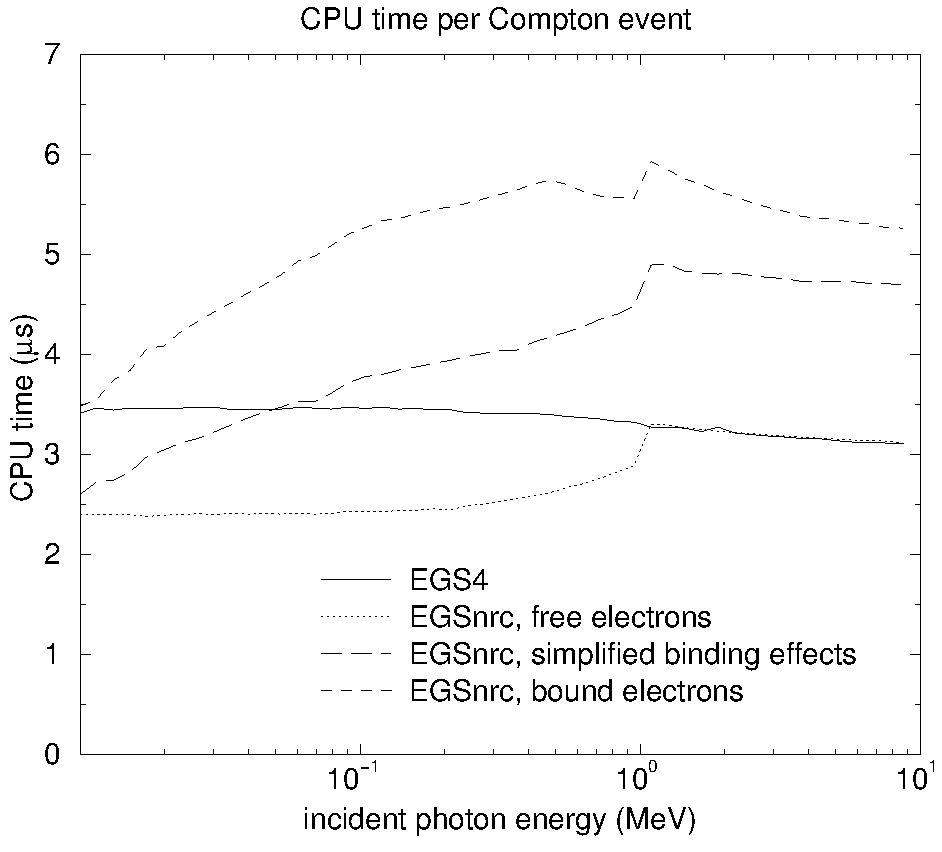
\includegraphics[height=12cm,width=12cm]{figures/comp_times}
\caption[CPU times for Compton sampling]{\label{comp_times}
CPU time in $\mu$s on a 500 MHz PIII computer to sample an incoherent
scattering event (including necessary rotations of particle directions).}
\end{figure}
Fig. \ref{comp_times} shows the CPU time per incoherent scattering event
for EGS4 (solid line), EGSnrc without (dotted line)
and with binding effects (dashed line) as a function of the incident
photon energy. The long dashed line would result if the function
$F(k,\cos \theta,p_z)$ was ignored. EGSnrc without binding effects is
faster than EGS4 for low photon energies due to the use of
the uniform sampling technique. The inclusion of binding effects
increases the CPU time per Compton event by not more than a
factor of two and so has only a minor effect on the overall simulation
time when electron transport is included. Binding effects and
Doppler broadening for coherent scattering are therefore turned
on by default in the {\tt block data} sub-program (the switch
{\tt IBCMP} is set to 3, {\tt norej}).
\index{IBCMP}

Since the 2009 release of EGSnrc, the user has the option to change
the EGSnrc behavior with respect to Compton interactions by
setting {\tt ibcmp=2} or {\tt ibcmp=3}.
When {\tt ibcmp=2}, binding effects are taken into account via an
incoherent scattering function, but there is no Doppler broadening.
This option was mainly added for the sake of being able to study the
effect of Doppler broadening by comparing simulations with
{\tt ibcmp=2} to {\tt ibcmp=1}. To select this option the user
must set {\tt Bound Compton scattering} to {\tt simple} in the
{\tt MC TRANSPORT PARAMETER} input block.
The {\tt ibcmp=3} option is the same as {\tt ibcmp=1}, but now the actual total
bound Compton cross section
is used and there are no rejections at run time. The addition of this option
was motivated by the complications associated with the initial bound
Compton scattering approach when using an un-weighting technique to compute
ion chamber correction factors for photon attenuation.
To select this option the user
must set {\tt Bound Compton scattering} to {\tt norej} in the
{\tt MC TRANSPORT PARAMETER} input block.

\index{Russian Roulette}
\index{variance reduction!Russian Roulette}
\index{incoherent scattering!Russian Roulette}
If the Russian Roulette option is turned on {\tt i\_play\_RR} set
to 1, electrons produced as a result of the Compton interaction
(the Compton electron and electrons from the relaxation of
the shell vacancy) are removed from the stack with the probability
{\tt prob\_RR}. If they survive, their weight is increased by
1/{\tt prob\_RR}.

\paragraph{Radiative Compton corrections}\hfill
\index{radiative Compton corrections}
\label{radc_corrections}

Recently, the code has been modified to also allow the user to include
radiative corrections for Compton scattering in the one-loop approximation.
These corrections are based on the original
Brown \& Feynman equations \cite{BF52}. The effect of loop corrections is to
reduce the cross section at large photon scattering angles. This is partially
offset by the addition of the double-Compton scattering process (two photons in
the final state). Devising an efficient technique for sampling energies and
directions from the double-Compton cross section is the most difficult part
in the implementation. The method is quite involved and its detailed description
awaits a future version of this report.

In order to turn on radiative corrections, the input variable
\index{radc\_flag}
\texttt{radc\_flag} (in the common block \texttt{COMIN/COMPTON-DATA}) must be set to 1.
This option can be enabled in applications which can read the \texttt{MC transport parameter}
input block from an input file (\texttt{*.egsinp}) via the input key:
\begin{verbatim}
   Radiative Compton corrections = on
\end{verbatim}
Moreover, one must include the file \texttt{\$(EGS\_SOURCEDIR)rad\_compton1.mortran} to the
list of MORTRAN sources to be built just before \texttt{\$(EGS\_SOURCEDIR)get\_inputs.mortran}.
Depending on the application type this is accomplished in different ways:

\begin{itemize}
 \item
  For all C++ applications one must edit the file \texttt{\$HEN\_HOUSE/specs/egspp1.spec}
  and include the above file in the definition of the \texttt{C\_ADVANCED\_SOURCES}
  variable if the application is derived from the \texttt{EGS\_AdvancedApplication} class or the
  \texttt{C\_SIMPLE\_SOURCES} variable for any application derived from the \texttt{EGS\_SimpleApplication} class.
 \item
  For a specific C++ application one could define the variable \texttt{CPP\_SOURCES} in the application's
  \texttt{Makefile} in the same manner as done above for the \texttt{C\_ADVANCED\_SOURCES}.
 \item
  For a \texttt{BEAMnrc} application one must edit the file \texttt{sources.make} located in the application's
  folder and include the above file in the definition of the \texttt{SOURCES} variable
  or the \texttt{LIB\_SOURCES} variable if this \texttt{BEAMnrc} application will be used as a particle source for
  another application.
 \item
  For a MORTRAN application named for instance \texttt{app} one must edit the corresponding file app.make located
  in the application's folder \texttt{\$EGS\_HOME/app} and include the above file
  in the definition of the \texttt{SOURCES} variable.
\end{itemize}

% Note that if radiative Compton corrections are to be used then the \texttt{Makefile} of
% the user code must be modified to include the file \texttt{\$(EGS\_SOURCEDIR)rad\_compton1.mortran}
% in the \texttt{SOURCES} list, just before\\
% \texttt{\$(EGS\_SOURCEDIR)get\_inputs.mortran}.

\paragraph{Total Compton cross sections}\hfill
\label{comp_xsect}
\index{bound Compton scattering!user-supplied cross sections}

As mentioned above, the total Compton cross section used in EGSnrc is obtained
from the theoretical expressions by integration of the differential cross sections.
Another recent addition to the EGSnrc code allows the user to supply their
own cross sections for bound Compton scattering. This option is only available
if the user is simulating bound Compton scattering
\index{IBCMP}
({\tt IBCMP}=1,2,3).  The cross sections
must be contained in a file\\
 {\tt \$HEN\_HOUSE/data/comp\_xsections\_compton.data},
where {\tt comp\_xsections} is the variable
(in common block {\tt COMIN/MEDIA}) holding the name as supplied
by the user.
\index{comp\_xsections}

\subsubsection{Photo-electric absorption}
\setcounter{equation}{0}
\label{photo}
\index{photo-electric absorption}

In the photo-electric absorption process a photon is
absorbed by an atom and an electron
is emitted with an energy given by the incident photon
energy minus its binding energy.
The atom, left in an excited state with a vacancy in the
ionized shell, relaxes via the emission of fluorescent photons and
Auger and Coster-Kronig electrons.

\index{fluorescent X-rays}
In the original default EGS4 implementation the emission of relaxation
particles following photo-electric absorption events was
ignored. This approach was later modified
to include the production of $K_\alpha$ and $K_\beta$ fluorescent
radiation. However, for incident photon energies below
the $K$-shell binding energy, the entire photon energy is
deposited locally. Another shortcoming of the EGS4 approach is
that the $K$-shell binding energy is always subtracted
from the energy of the electron set in motion, even though there
is a certain probability that the photo-absorption process
takes place with a shell other than the $K$-shell (for
high-$Z$ materials this probability is of the order of 20\%).
Finally, the use of the fluorescent option in EGS4 requires
the user to select an ``effective'' atomic number for each
material. The photo-absorption then always takes place with
this atomic number. The meaningful selection of an
``effective'' $Z$ proves to be a difficult task for mixtures, especially
when only a small fraction of a high-$Z$ element is present.

\index{cross section!photo-electric absorption}
Although this release of EGSnrc uses the total photo-absorption
cross sections from PEGS (which are taken from the
compilation by Storm and Israel \cite{SI70})
the simulation of the photo-absorption process
is completely changed and is controlled
by the flag {\tt IEDGFL}
(in the {\tt COMIN/EDGE} common block-see Section~\ref{common_blocks}). If {\tt IEDGFL} of the
region is non-zero, a detailed simulation is performed,
otherwise a simplified treatment of the photo-absorption process
is undertaken. The default setting of {\tt IEDGFL} is 1.
\index{IEDGFL}

\paragraph{Detailed simulation of photo-electric absorption}\hfill
\label{photo_detailed}
\index{photo-electric absorption!detailed simulation of}

\begin{enumerate}
\item
For compounds and mixtures, the first step is to sample the
atomic number of the element the
photon is interacting with.
If $Z_i$ denotes the atomic number of the $i$'th element in
the molecule, $p_i$ its stoichiometric index, and
$\sigma_{\rm ph}(k,Z)$ the photo-electric absorption
cross section for a photon of energy $k$ by an element
with atomic number $Z$, then the probability $w_i(k)$ that
the photon is absorbed by the element $Z_i$ is
\begin{equation}
w_i = {p_i \sigma_{\rm ph}(k,Z_i) \over \sum p_i \sigma_{\rm ph}(k,Z_i)}~.
\end{equation}
The sampling of the element therefore requires the knowledge of
all elemental photo-absorption cross sections at run time, not
just the total photo-absorption cross sections that comes from
the PEGS data set. To minimize the amount of additional data
required, we use fit formulas for the $\sigma_{\rm ph}(k,Z_i)$'s
which are accurate to within 1-2\% and have the form
\begin{eqnarray}
\sigma_{\rm ph}(k,Z) & = & \frac{A_K(Z)}{k} + \frac{B_K(Z)}{k^2} +
\frac{C_K(Z)}{k^{7/2}} + \frac{D_K(Z)}{k^4}~, \quad \mbox{if}~k \ge U_K(Z)
\\
%& = & \exp \left[A_j(Z) + B_j(Z) \ln k + C_j(Z) (\ln k)^2 + D_j(Z) (\ln k)^3
%\right]~, \quad \mbox{else if}~k \ge U_j(Z)
& = & \exp \left[A_j(Z) + B_j(Z) t + C_j(Z) t^2 + D_j(Z) t^3
\right]~, \quad \mbox{else if}~k \ge U_j(Z)
\nonumber
\end{eqnarray}
where $t = \ln k$ and where $U_K(Z)$ is the
$K$-shell binding energy and $U_j(Z)$ binding
energies for shells other then the $K$-shell. We have obtained The
coefficients $A_K, B_K, ...$ and $A_j, B_j, ...$
by fitting the photo-absorption cross sections from the {\tt XCOM} program
\cite{BH87} and are found in the file {\tt photo\_cs.data}
(only shells with a binding energy above 1 keV are included).
The algorithm to select the element that absorbs the
incident photon is then:
\begin{itemize}
\item[1.1] Calculate all $\sigma_{\rm ph}(k,Z_i)$ and
their sum
\item[1.2] Pick a random number $r_1$
\item[1.3] In a loop over the number of elements, calculate
$r_1 = r_1 - w_i$, if $r_1 \le 0$ exit the loop and take
$Z_i$ as the element interacting with the photon.
\end{itemize}
Note that, at least in principle,
\begin{displaymath}
\sum p_i \sigma_{\rm ph}(k,Z_i) = \sigma_{\rm ph}(k)
\end{displaymath}
where $\sigma_{\rm ph}(k)$ is the photo-absorption cross section
for the material under consideration. This cross section is
interpolated using the PEGS supplied data in the photon
transport routine in order to determine
the interaction type. One could make the element selection algorithm
more efficient by employing
\begin{itemize}
\item[1.1']
Pick a random number $r_1$
\item[1.2']
Set $i=1$
\item[1.3']
Calculate $\sigma_{\rm ph}(k,Z_i)$ and
$r_1 = r_1 - p_i \sigma_{\rm ph}(k,Z_i)/\sigma_{\rm ph}(k)$.
\item[1.4'] If $r_1 > 0$ and $i$ less then the number of elements,
then $i = i+1$, go to step 1.3'.
\item[1.5'] Deliver $i$.
\end{itemize}
as this saves the evaluation of one or more $\sigma_{\rm ph}(k,Z_i)$
(especially if elements are ordered by decreasing probability for
photo-absorption prior to the actual simulation). We have not
implemented this more efficient algorithm as the photo-absorption
cross section interpolated using the PEGS supplied data becomes
inaccurate around absorption edges. This potential improvement is
left for future releases of the system (which are anticipated to
not make use of PEGS data sets).
\item
Once the absorbing element is determined, the shell
with which the interaction takes place has to be sampled.
The probability $\nu_j$ that the photon is absorbed by the $j$'th shell
is close to energy independent for the $K$-shell but depends
on the incident photon energy for other shells. This means that
shell-wise photo-absorption cross sections would be required
to be available at run time in order to sample the shell
if one wanted to perform a complete modeling of the
photo-absorption process. In this release of the EGSnrc system
we use instead energy independent interaction probabilities $\nu_j$
which are determined as follows. If $\phi(k)$ is the
fluence of the photon radiation field, the number of photo-absorption
events by the element $Z$ per unit volume, $N$, is given by
\begin{equation}
N = n(Z) \int {\rm d} k \phi(k) \sigma_{\rm ph}(k,Z)
\end{equation}
where $n$ is the density of scattering centers.
The number of photo-absorptions by the shell $j$ of this
element per unit volume is
\begin{equation}
N_j = n(Z) \int {\rm d} k \phi(k) \sigma_{{\rm ph},j}(k,Z)
\end{equation}
where $\sigma_{{\rm ph},j}(k,Z)$ is the photo-absorption cross section
of the $j$'th shell. The ratio of $N_j$ to $N$ is the average
interaction probability for absorption by the $j$'th shell, $\nu_j'$,
for the radiation field described by $\phi(k)$,
\begin{equation}
\nu_j' = \frac{N_j}{N} = {\int {\rm d} k \phi(k) \sigma_{{\rm ph},j}(k,Z)
\over \int {\rm d} k \phi(k) \sigma_{\rm ph}(k,Z) }
\end{equation}
The actual quantity used in the simulation of photo-electric absorption
is the probability $\nu_j$ that the photon is absorbed by the
shell $j$  if it was not absorbed by one of the shells $1 \cdots j-1$,
which is given by
\begin{equation}
\label{photo_nuj}
\nu_j = {\int {\rm d} k \phi(k) \sigma_{{\rm ph},j}(k,Z) \over
\sum_{i=j}^{N_{\rm sh}} \int {\rm d} k \phi(k) \sigma_{{\rm ph},i}(k,Z)}
\end{equation}
where $N_{\rm sh}$ is the total number of shells.
To calculate $\nu_j$ one needs $\phi(k)$, a quantity that
is not known (but intended to be calculated by the Monte
Carlo simulation). Nevertheless, one could calculate
$\nu_j$ by making a guess about the photon fluence, this
approach is the basis for the generation of group interaction
coefficients for discrete ordinate methods (see {\em e.g}
the book by Lewis and Miller \cite{LM84}).
\begin{figure}[h]
%\setlength{\vsize}{12cm}
%\setlength{\abovecaptionskip}{0.5in}
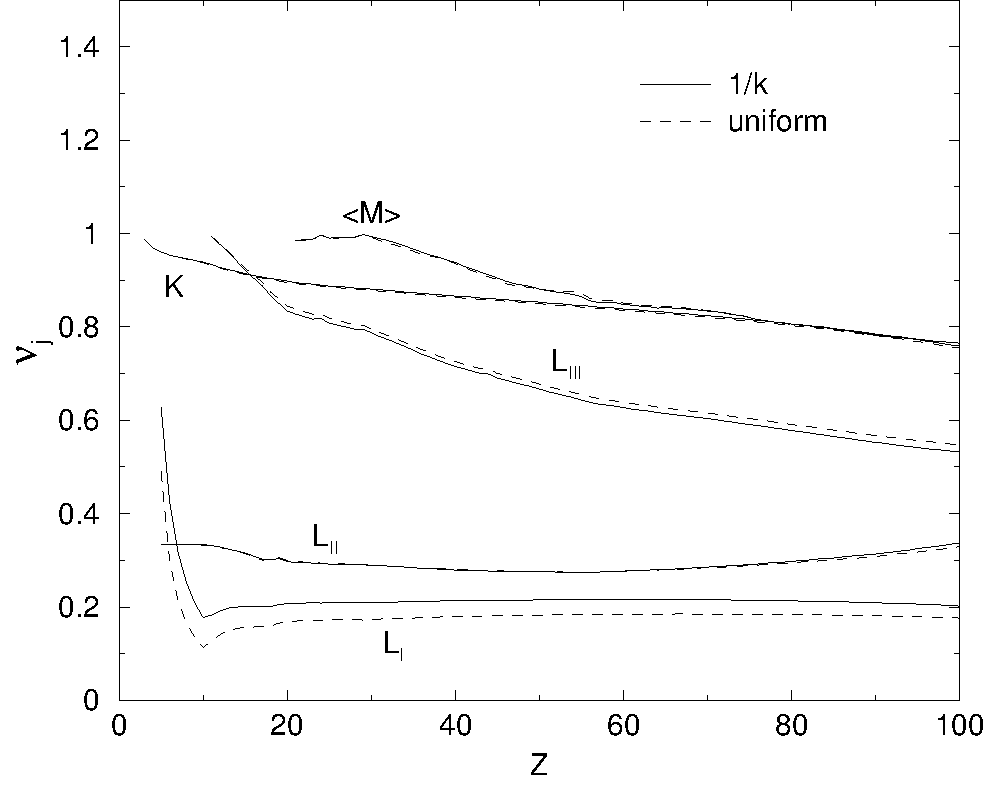
\includegraphics[height=12cm,width=12cm]{figures/intp}
\caption[Interaction probabilities for different shells]{\label{phot_intp}
Interaction probabilities $\nu_j$ for different shells as
calculated from Eq. (\protect\ref{photo_nuj}) using
$\phi(k)=1/k$ (solid lines) or $\phi(k)=\mbox{const}$ (dashed lines).}
\end{figure}
Figure \ref{phot_intp} shows the interaction probabilities
$\nu_j$ of the $K, L_I, L_{II}$ and  $L_{III}$ shells and an
``average'' $M$ shell (see next paragraph)
as a function of the
atomic number $Z$ for $\phi(k) = \mbox{const}$ (dashed line)
and $\phi(k) = \mbox{const}/k$ (solid line).
Shell-wise photo-absorption cross section from
the Evaluated Photon Data Library (EPDL) \cite{Cu89}
were used to generate this figure, the upper limit of
the $k$-integration was set to 1 MeV. The dependence of
the $\nu_j$s on the weighting function $\phi(k)$ is
negligible except for the $L_I$ shell where the difference
is of the order of 10\%. This fact was the motivation for
using the energy independent interaction probabilities $\nu_j$,
a better approach is scheduled for a future release of the
system.

The use of an interaction probability for an ``average'' $M$-shell
is motivated by the fact that relaxation transitions from and to
$M$-shells are treated in an average way, see section \ref{relax}.
Given the definition of the $\nu_j$'s, $\nu_{\langle M \rangle}$ is
\begin{equation}
\nu_{\langle M \rangle} = 1 - \prod (1 - \nu_{M_i})
\end{equation}
where the product runs over the number of $M$-sub-shells available
for the element $Z$ (up to 5). The interaction probabilities
$\nu_K, \nu_{L_I}, \nu_{L_{II}}, \nu_{L_{III}}$ and $\nu_{\langle M \rangle}$,
calculated with the $1/k$ weighting function, are stored in the
file {\tt photo\_relax.data} and read in by the subroutine
{\tt edgset} which is called from {\tt HATCH}.

With all this, the algorithm for selecting the shell that absorbs
the incident photon is as follows:
\begin{itemize}
\item[2.1]
Determine the inner-most shell $j$ that has a binding energy lower
than the incident photon energy and pick a random number $r_2$
\item[2.2]
If $r_2 < \nu_j$ or $j > \langle M \rangle$
\footnote{The outer-most shell treated is the $M$ shell, if the photon
was not absorbed by it, it is assumed that it is absorbed by the
$N$ shell.}, then deliver $j$
\item[2.3]
Set $r_2 = (1 - r_2)/(1 - \nu_j),~j = j+1$, go to step 2.2
\end{itemize}
\item
Once the element and its shell absorbing the photon is determined,
a photo-electron with the kinetic energy $k - U_j(Z)$ is set-up, where
$U_j(Z)$ is the binding energy of the selected shell.
The vacancy created is treated in the routine ({\tt relax}, see section
\ref{relax}),
this significant change compared to EGS4 is motivated by the
fact that shell vacancies are created also
in other processes, {\em e.g.} Compton scattering (see section \ref{compton}).
The sampling of the photo-electron direction is discussed in section
\ref{photo_direction}.
\end{enumerate}

\paragraph{Simplified simulation of photo-electric absorption}\hfill
\label{photo_simple}
\index{photo-electric absorption!simplified simulation of}

If the flag {\tt IEDGFL} for the current region is set to zero,
a simplified simulation of the photo-absorption process is undertaken.
This simplified treatment consists of one step:
\index{IEDGFL}
\begin{enumerate}
\item
Set-up a photo-electron with a kinetic energy $k$
\end{enumerate}
There are several reasons which motivated us to change the
logic compared to the current EGS4 version (where the
$K$-shell binding energy is always subtracted):
\begin{itemize}
\item
The treatment is greatly simplified
\item
If the flag {\tt IEDGFL} is set to zero, it is reasonable to assume
that the detailed calculation of the spread of energy released
in photo-absorption events is not important for the situation
under investigation
\item
The effect of the production of relaxation particles in the
de-excitation cascade following photo-electric absorption is
to spread out the binding energy around the point of interaction.
By giving the photo-electron the entire incident photon energy,
this effect is at least partially simulated.
\end{itemize}

\paragraph{Photo-electron direction}\hfill
\label{photo_direction}
\index{photo-electric absorption!direction of electron}

\index{IPHTER}
The behavior of the sampling of the photo-electron direction
is controlled by the switch {\tt IPHTER}
(included in the {\tt COMIN/EDGE} common block) which set on a
region by region basis. If set to zero,
the photo-electron ``inherits'' the direction of the incident
photon. If set to non-zero (the default selection),
the direction is sampled from the
Sauter distribution \cite{Sa31}. The implementation as discussed
in detail in Ref. \cite{BR86a} is adopted. For completeness, we give a
brief summary here.
\index{Bielajew, Alex}

Sauter's distribution in the polar angle
$\mu = \cos \theta$ with respect to the incident
photon direction may be cast in the form \cite{BR86a}
\begin{equation}
f(\mu) {\rm d}\mu = {1 - \mu^2 \over (1 - \beta \mu)^4} \left[ 1 +
\kappa (1 - \beta \mu) \right] {\rm d} \mu
\end{equation}
where $\beta$ is the electron's velocity in units of the
speed of light  and
\begin{equation}
\kappa = {\gamma \over 2} (\gamma - 1) (\gamma - 2)~, \quad \gamma =
{1 \over \sqrt{1 - \beta^2} }
\end{equation}
This equation can be sampled by generating candidate
$\mu$ values from
\begin{equation}
g(\mu) = {1 \over 2 \gamma^2 (\kappa + \gamma)^2} ~{
1 + \kappa (1 - \beta \mu) \over (1 - \beta \mu)^2 }~,
\end{equation}
which is a normalized PDF for $\mu$, and using
\begin{equation}
h(\mu) = { \gamma + 1 \over 2 \gamma } ~{1 - \mu^2 \over 1 - \beta \mu }
\end{equation}
which is always positive and has a maximum of unity,
as a rejection function. To generate $\mu$ values from
$g(\mu)$, one uses
\begin{equation}
\mu = {1 \over \beta} \left[1 - \left( \sqrt{\left(\kappa + {1 \over 1 + \beta}
\right)^2 + 4 \beta \gamma^2 (\kappa + \gamma^2) r_1} - \kappa \right)^{-1}
\right]
\end{equation}
where $r_1$ is an uniformly distributed random number.

\index{Sauter distribution}
It is worth noticing that, strictly speaking, Sauter's distribution is
valid only for the $K$-shell and also derived
from an extreme relativistic approximation. The treatment
of the photo-electron angular distribution is therefore left
as a macro {\tt \$SELECT-PHOTOELECTRON-DIRECTION;}
and can therefore be replaced, if the user has a better approach.
\index{\$SELECT-PHOTOELECTRON-DIRECTION}

\subsubsection{Coherent (Rayleigh) scattering}
\label{rayleigh}
\setcounter{equation}{0}
\index{Rayleigh scattering}
\index{coherent scattering}
\index{cross section!coherent}

Originally, EGSnrc ``inherited'' the treatment of the coherent
photon scattering process from EGS4 \cite{Ne85}.
This means that the total coherent scattering cross
sections from Storm and Israel \cite{SI70} and the atomic
form factors $F_T(q,Z)$ from Hubbel and {\O}verb{\o} \cite{HO79} are used
by default.
The form factors for molecules are calculated from the independent
atom approximation, {\em i.e.}
\begin{equation}
[F_T(q)]^2 = \sum p_i [F_T(q,Z_i)]^2
\end{equation}
where $p_i$ is the stoichiometric index of the $i$'th element,
$Z_i$ its atomic number and $q$ the momentum transfer when
a photon with an energy $k$ is scattered by an angle $\theta$,
\begin{equation}
q = k \sqrt{{1 - \cos \theta \over 2}}~.
\end{equation}
The coherent scattering cross section, differential in the
photon angle $\Omega = (\theta, \phi)$ is
\begin{equation}
{{\rm d} \sigma_{\rm R} \over {\rm d} \Omega} = {r_0^2 \over 2}
(1 + \cos^2 \theta) [F_T(q)]^2~.
\end{equation}
This equation is sampled by re-writing it in terms of
$q^2$,
\begin{equation}
{{\rm d} \sigma_{\rm R} \over {\rm d} q^2} = {4 \pi r_0^2 \over k^2}~
A(q_{\rm max}^2)~
{1 + \cos^2 \theta \over 2} ~{[F_T(q)]^2 \over A(q_{\rm max}^2)
}
\end{equation}
where
\begin{equation}
A(q^2) = \int\limits_0^{q^2} {\rm d}q^{'2} [F_T(q')]^2
\end{equation}
and $q_{\rm max} = k$ is the maximum possible momentum transfer, and
using $[F_T(q)]^2/A(q_{\rm max}^2)$  as a PDF for $q^2$ and
$(1 + \cos^2 \theta)/2$ as a rejection function.

\index{coherent scattering!sampling of}
\index{IRAYLR}  \index{\$RAYLEIGH-SCATTERING;}
The actual sampling, accomplished in the macro
{\tt \$RAYLEIGH-SCATTERING;}, is performed only
if the switch {\tt IRAYLR} (included
in the {\tt COMIN/MISC} common block--see Section~\ref{common_blocks})
is set to non-zero for the current
region. By default, {\tt IRAYLR} is set to zero in the {\tt
block data} subprogram. The motivation for this choice is
the fact that the {\tt \$RAYLEIGH-SCATTERING;} macro
requires the function $A(q^2)$ to be included in the PEGS data
set. This additional data is only included, if the user specifically
requested it from PEGS.

We recommend the Rayleigh
scattering option to be used for low energy calculations
(say, below 1 MeV). It is worth noticing that
inclusion of coherent scattering without the use
of the bound Compton scattering option (see section \ref{compton})
results in too much photon scattering, binding effects
for incoherent scattering should therefore always be turned
on if the Rayleigh option is used.

\paragraph{New coherent scattering angular sampling}\hfill
\label{new_rayleigh_sampling}

\index{Rayleigh scattering!new angular sampling}
% The above sampling algorithm approximates the angular distribution
% for coherent scatter relatively well. However,
% the forward peaked shape of $[F_T(q)]^2/A(q_{\rm max}^2)$
% and its uniform sampling in equidistant intervals
% between 0 and 1 translates into a non-uniform sampling
% of the scattering angle since larger angular intervals
% are covered with increasing bin number. As a consequence,
The original EGS4 sampling algorithm produces a step-like averaging
artifact at large angles, which increases with energy. This is
shown by the symbols in Figure \ref{ray_ang_sampling_fig}, for
20 keV, 60 keV and 110 keV photon beams in water.
However, this artifact has no practical consequences, unless one is
interested in the few photons scattered at large angles.
\begin{figure}[h]
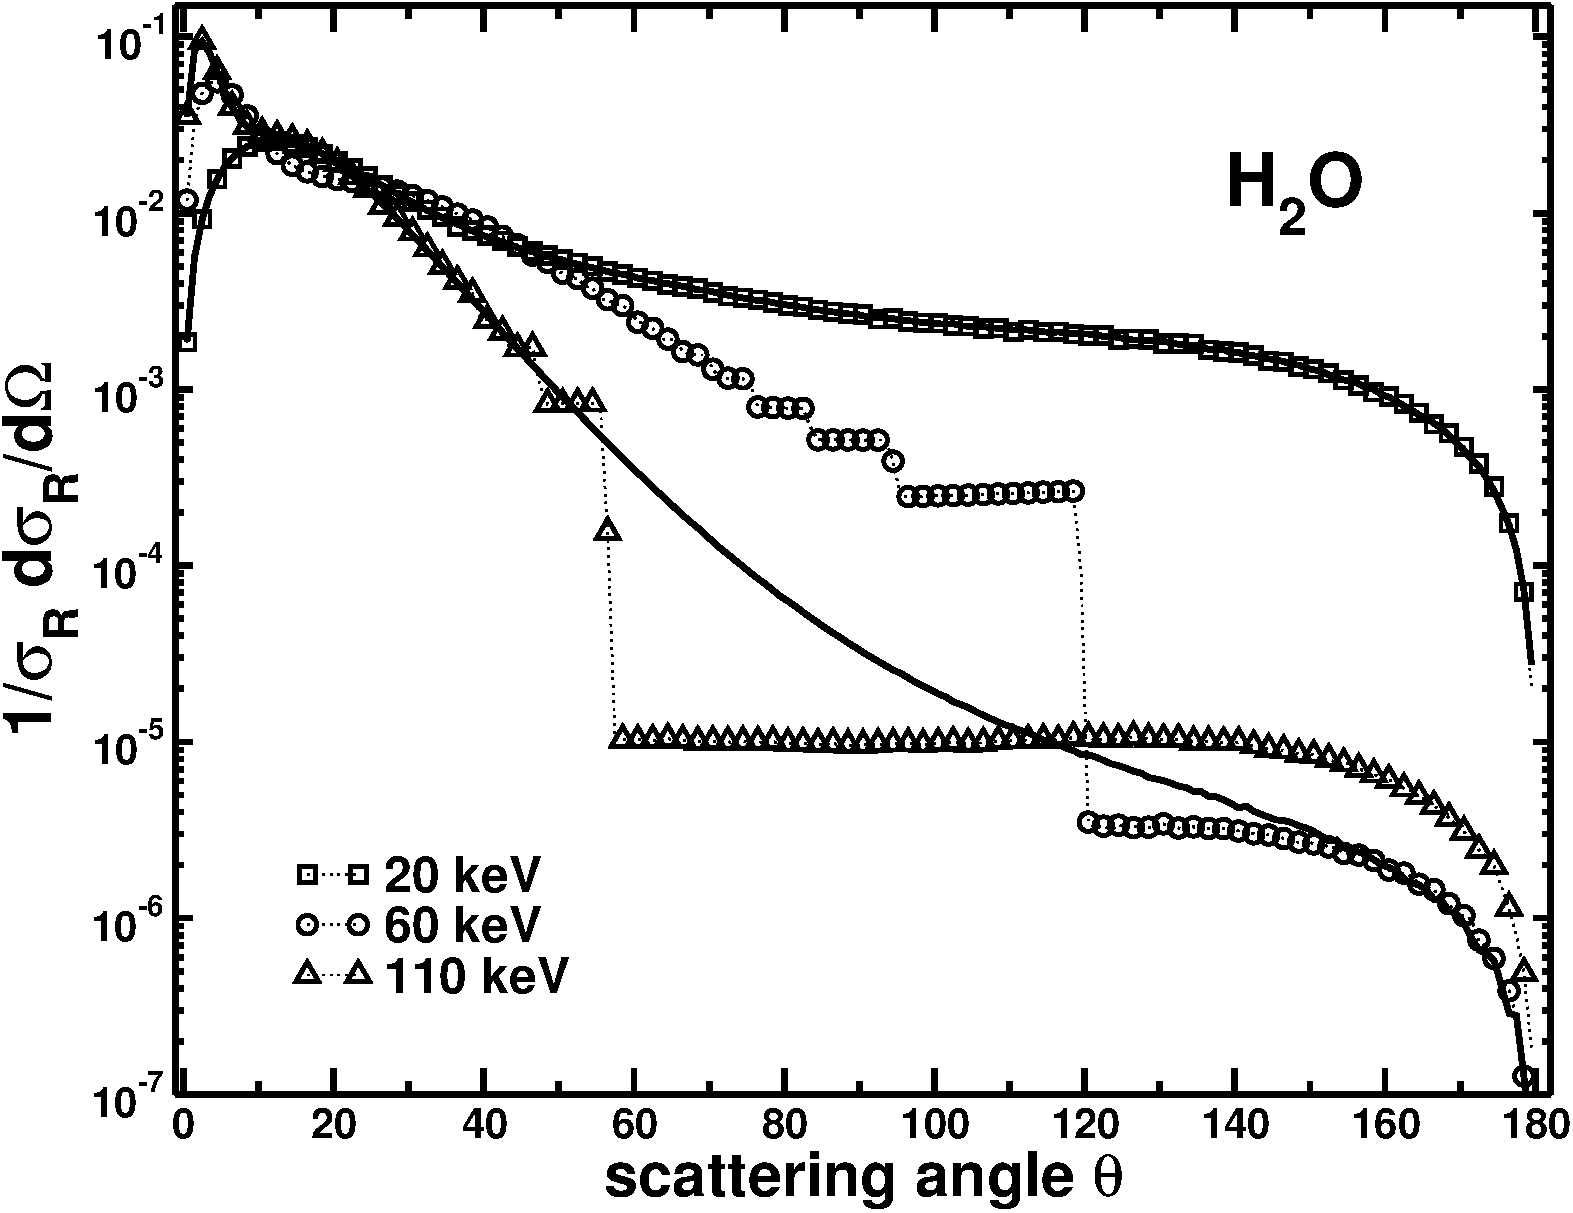
\includegraphics[height=9cm,width=9cm]{figures/ray_ang_dist_old_vs_new}
\caption[Angular distribution of coherently scattered photons for 20 keV, 60 keV
and 110 keV photon beams in water.]{\label{ray_ang_sampling_fig}
Angular distribution of coherently scattered photons for 20 keV, 60 keV
and 110 keV photon beams in water. Symbols represent the original EGS4
sampling algorithm and the solid lines the new alias sampling.
}
\end{figure}

The default angular sampling algorithm for coherent scattering
was replaced in 2007 for an alias-sampling algorithm that properly
samples $[F_T(q)]^2/A(q_{\rm max}^2)$ removing this artifact as shown
by the solid lines in Figure \ref{ray_ang_sampling_fig} for 20 keV
and 110 keV. The coherent scattering form factors are now
read directly either from {\tt \$HEN\_HOUSE/pegs4/pgs4form.dat}
(default atomic form factors, see section \ref{rayleigh} above) or from
user-supplied form factor files expected to be in the
{\tt \$HEN\_HOUSE/data/molecular\_form\_factors/} directory
(see section \ref{custom_ff_sect} below for more details).
This means that one can now switch on coherent (Rayleigh) scattering,
even if there is no Rayleigh data in the PEGS4 data set.

The old sampling macro is now named {\tt \$OLD\_RAYLEIGH-SCATTERING;}.
If one is interested
in reproducing old calculations or just want to use the old sampling,
this macro could be renamed back to {\tt \$RAYLEIGH-SCATTERING;}.
Please note that in this case a PEGS4 file is required with the needed
interpolation coefficients and the input key {\tt Photon cross sections}
in the {\tt MC transport parameters input block} must be set to {\tt PEGS4}
(see section \ref{xsections}, page~\pageref{xsections}).

\paragraph{Custom atomic and molecular form factors}\hfill
\label{custom_ff_sect}
\index{Rayleigh scattering!custom form factors}

\index{iray\_ff\_file}\index{iray\_ff\_media}
The user now has the option of supplying their own custom atomic
or molecular form factors for determining Rayleigh cross sections.
These are specified through the {\tt iray\_ff\_media} (medium names) and
{\tt iray\_ff\_file} (files containing form factor data)
variables contained in the
{\tt COMIN/RAYLEIGH\_INPUTS} common block.
\index{RAYLEIGH\_INPUTS common block}
A number of measured molecular form factors from the work by
Peplow and Verghese \cite{PV98} are distributed with EGSnrc and can be
found in the {\tt \$HEN\_HOUSE/data/molecular\_form\_factors} directory.

To enable this option, one needs to set the input key {\tt Rayleigh scattering}
to {\tt custom} in the {\tt MC transport parameters} input block. An example
of such an input is shown below:

\begin{verbatim}
:start MC transport parameter:
  .
  .
  .
  Rayleigh scattering=  custom
  ff media names = BREASTICRU512 \
                   FATICRU512 \
                   MUSCLEICRU512 \
                   KAPTONICRU512
  ff file names = /ff_file_location/mff_breast_tissue.dat \
                  /ff_file_location/mff_pork_fat.dat \
                  /ff_file_location/mff_pork_muscle.dat \
                  /ff_file_location/mff_kapton.dat

:stop MC transport parameter:
\end{verbatim}

Note that since there is no check, the user must make sure that the medium name and
the form factor file correspond to the same material.

\subsubsection{Changing photon cross sections}
\label{photon_xsect}
\index{photon cross section data!changing}
\index{photon\_xsections}
\index{XCOM}
\index{EPDL}
\index{Storm \& Israel}

In the current version of EGSnrc, the user has the option to use
photon cross section data other than the default
Storm \& Israel data.  To do this, the user must
set the character variable {\tt photon\_xsections} (part of the
{\tt COMIN/MEDIA} common block) to the name of the cross section
data to use.  Cross sections included with the EGSnrc distribution
are: 1) the Evaluated Photon Data
Library\cite{Cu97a} (set {\tt photon\_xsections= "epdl"})
2) XCOM data from Berger \& Hubbell\cite{BH87} (set {\tt photon\_xsections= "xcom"}
-- also the default in the absence of any input)
and 3) Storm \& Israel\cite{SI70} (set {\tt photon\_xsections= "si"}). For information on how
to set the variable {\tt photon\_xsections}, the reader
is referred to section~\ref{step_2} (page~\pageref{photon_xsections_description}).

The user can also supply their own photon cross section data.
This can be accomplished by placing data files named
{\tt xxxx\_photo.data, xxxx\_pair.data, xxxx\_triplet.data} and {\tt xxxx\_rayleigh.data}
in the {\tt \$HEN\_HOUSE/data} folder, where {\tt xxxx} stands for any string different
from {\tt epdl, xcom} or {\tt si}. These cross sections will then be used if
the variable {\tt photon\_xsections} is set to {\tt xxxx}. The format of the
ASCII data files is very simple: for each element between 1 and 100 one has to
provide the number $N$ of data points in the tabulation followed by $N$
pairs of the logarithm of the photon energy in MeV and the logarithm of the
cross section in barn (see also one of the data files provided with EGSnrc).

Since 2006 EGSnrc was modified to ignore the photon data in the PEGS4
file, re-initializing all interpolation tables to utilize the
maximum number of interpolation bins availble. In this way, the user
can minimize the inaccuracies around atomic edges by replacing \$MXGE with
a huge number in their user code. Starting with the 2011 release
(V4 release 2.3.2), the use of PEGS4 photon data has been re-enabled for
backwards compatibility.
To achieve this, the user must set the character variable
{\tt photon\_xsections} to {\tt PEGS4} (case insensitive). See
section \ref{xsections} (page~\pageref{xsections}) for more
information on this topic.

It is worth noting that the total cross section for Compton scattering is
normally obtained from the theoretical differential cross section being used
(Klein-Nishina or RIA, see section \ref{compton}) by
integrating over the kinematically allowed range instead of being taken from
tabulations. This behavior can be changed by the user as described in
section \ref{compton}).

\subsection{Atomic Relaxations}
\label{relax}
\index{atomic relaxations}
\index{relaxations}
\index{fluorescent X-rays}
\index{Auger transitions}
\index{Coster-Kronig transitions}

Excited ions, produced by the interaction of photons and
charged particles when they travel through matter, relax to
their ground state by migration of the initial vacancy to
outer shells via the emission of characteristic X-rays and/or
Auger or Coster-Kronig electrons (see {\em e.g.} Ref. \cite{Pe91}).

In the current standard version of EGS4, only $K$-shell relaxations following
photo-electric absorption via
the emission of $K_\alpha$ and $K_\beta$ fluorescence are treated
and are intrinsically associated with the {\tt PHOTO} routine.
An extension to include $L$-shell fluorescence was developed by the
KEK group \cite{Na98} and is available for use with the EGS4 system.

In EGSnrc we have extended the treatment of atomic relaxations
to include higher shells as well as the production of Auger and
Coster-Kronig electrons. With these extensions, the
treatment within the {\tt PHOTO} routine
has become unpractical. In addition, the relaxation cascade
is a separate process, it can be initiated after any photon
or electron interaction that has produced an inner shell vacancy.
The most general approach for treating excited atoms or ions would have
been to define a separate particle type, an excited atom or ion, and to
put such particles on the stack whenever they are produced.
Such an approach would have been too a large departure from
the EGS4 logic and potentially render many user codes unusable.
We have therefore abandoned this idea and decided to
treat relaxations in a separate routine ({\tt relax}),
which is called whenever an inner shell vacancy is created.
In this release of EGSnrc, such vacancies can be created in
photo-absorption events (see section \ref{photo}) and in
Compton scattering events (see section \ref{compton}).
It is anticipated that the next release of the system
will include the explicit modeling of inner shell
ionizations by electron or positron impact.

\index{low energy limit!photon}
\index{energy range}
\index{limitations!energy}
The de-excitation cascade is a complex process, there are
hundreds of possible transitions for high-$Z$ elements.
A complete treatment goes beyond the scope of a general
purpose code for the simulation of electron and photon transport
such as EGSnrc. In addition, we consider 1 keV to be the lowest
limit for the applicability of the code. We have therefore imposed
a lower limit of 1 keV on the relaxation process, {\em i.e.} only
vacancies in shells with binding energies
above 1 keV are treated.\footnote{Another motivation
for imposing this limit is the fact that uncertainties on
transition probabilities rapidly increase with
decreasing binding energies, they are perhaps 10 or 20\%
even for $L$-shells} If we then take into account that
only elements with $Z \ge 52$ have $M$-shells with binding energies
above the limit of 1 keV and that $M$-shells have binding energies less
than 10 keV for all elements (the $M_I$ binding energy for
lead is 3.8 keV and 7.2 keV for Einsteinium \cite{Pe91}),
it is a reasonable approach to model transitions from and
transitions to $M$-shells in an ``average'' way.
There is of course no unique procedure to set the binding energies of the
``average'' $M$-shells for the elements, $U_{\langle M \rangle}(Z)$,
to be used in the de-excitation cascade.
Assuming that for most applications $K$ to $M$ transitions
are more important than $L$ to $M$ or $M$ to a lower shell,
we have defined $U_{\langle M \rangle}(Z)$ to be the weighted average
of the binding energies $U_{M_j}(Z)$ of the element $Z$ with
weights given by the $K$ to $M_j$ transition probabilities $\nu_{KM_j}$,
\begin{equation}
U_{\langle M \rangle}(Z) \equiv {\sum \nu_{KM_j} U_{M_j} \over
\sum \nu_{KM_j}}
\end{equation}
For instance, $U_{\langle M \rangle}$ determined by this
procedure using transition probabilities from the
Evaluated Atom Data Library (EADL) \cite{Pe91} for lead
is 3.1 keV, the $M_I$ binding energy is 3.8 keV and the
$M_V$ binding energy 2.5 keV. A simple averaging with the
occupation numbers would result in an average $M$-shell binding
energy of 2.9 keV. If distinguishing between any of the above
numbers is important for your application, EGSnrc is most
likely not the most appropriate simulation package for
your purposes.
\index{limitations!M shell}

Having said all this, it is apparent that $N$ shells are
also treated in an average way. The only elements with
``average'' $N$-shell binding energies above 1 keV are those with $Z > 95$.

In an implementation consistent with the overall logic
of the EGS system, the relaxation algorithm should
put all particles produced in the course of the
de-excitation cascade on the particle stack, they would
then be discarded in the {\tt PHOTON} or {\tt ELECTR}
routines if their energies were below the specified
transport threshold energies. It is easy to see that
such an approach may become extremely wasteful if
the transport threshold energies are large compared to
the lower limit of 1 keV for the de-excitation cascade.
We have therefore decided to stop the relaxation process
for vacancies with binding energies less then $E_{\rm min}$,
\begin{equation}
E_{\rm min} = \mbox{Max} \{ 1~\mbox{keV},~\mbox{Min}
\{ {\tt PCUT}, {\tt ECUT} - m \} \}
\end{equation}
and to score their energy locally. In addition,
the energy of photons or electrons that are below
the thresholds are also deposited locally, even if
they were produced in transitions from vacancies
with binding energies above $E_{\rm min}$.
The total sub-threshold energy is collected in
the variable {\tt EDEP}, which is in the {\tt COMON/EPCONT/},
and made known to the
user via an {\tt IARG=4} call to the scoring routine.
\index{IARG!4}
\index{EDEP}

To facilitate the handling of the relaxation cascade, we
define a shell number $n$ for each of the shells treated.
$K$-shells have $n=1$, $L_I$ through $L_{III}$ have $n=2$ to 4,
$\langle M \rangle$ corresponds to $n=5$, $\langle N \rangle$ to
$n=6$, all other shells have $n=7$. A list of possible
transitions, $L_n$, is associated with each shell,
\begin{equation}
L_n = \{ (\nu_1, s_1), (\nu_2, s_2), \cdots, (\nu_{k_n}, s_{k_n}) \}
\end{equation}
where $k_n$ is the number of possible transitions for the shell
of type $n$ and $\nu_i$ the transition probabilities for
a transition into final state $s_i$.  The final states
$s_i$ are defined as follows:
\begin{equation}
s_i =
\left\{
\begin{array}{l@{\quad , \quad}l}
n_i & \mbox{for fluorescent transitions} \\
10 + n_i & \mbox{for Coster-Kronig transitions} \\
100 n_{i,1} + n_{i,2} & \mbox{for Auger transitions}
\end{array}
\right.
\end{equation}
where $n_i$ or $n_{i,1}$ and $n_{i,2}$ are the shell numbers of the
new vacancies created in fluorescent and Coster-Kronig or Auger transitions.
Table \ref{relax_transitions}
summarizes all transitions handled in the current version
of the relaxation routine.
\index{relaxation transitions}
%\begin{longtable}[htb]
\begin{table}[phtb]
\caption{\label{relax_transitions} Relaxation transitions handled
by EGSnrc.}
%\hline \hline
%initial vacancy & shell code & transition & final state code \\
%\hline \hline
%\endhead
%\hline \hline
%\endfoot
\begin{center}
\begin{tabular}{|c|c|c|c|}
\hline \hline
initial vacancy & shell code & transition & final state code \\
\hline \hline
 & & Fluorescent $K \to L_{II}$ & \phantom{00}3 \\
 & & \phantom{Fluorescent} $K \to L_{III}$ & \phantom{00}4 \\
 & & \phantom{Fluorescent} $K \to \langle M \rangle$ & \phantom{00}5 \\
 & & \phantom{Fluorescent} $K \to \langle N \rangle$ & \phantom{00}6 \\
 & & Auger $K \to L_I L_I$ & 202 \\
 & & \phantom{Auger} $K \to L_{II} L_{I}$ & 302 \\
 & & \phantom{Auger} $K \to L_{II} L_{II}$ & 303 \\
 & & \phantom{Auger} $K \to L_{III} L_{I}$ & 402 \\
 & & \phantom{Auger} $K \to L_{III} L_{II}$ & 403 \\
 $K$ & 1 & \phantom{Auger} $K \to L_{III} L_{III}$ & 404 \\
 & & \phantom{Auger} $K \to \langle M \rangle L_{I}$ & 502 \\
 & & \phantom{Auger} $K \to \langle M \rangle L_{II}$ & 503 \\
 & & \phantom{Auger} $K \to \langle M \rangle L_{III}$ & 504 \\
 & & \phantom{Auger} $K \to \langle M \rangle \langle M \rangle $ & 505 \\
 & & \phantom{Auger} $K \to \langle N \rangle L_{I}$ & 602 \\
 & & \phantom{Auger} $K \to \langle N \rangle L_{II}$ & 603 \\
 & & \phantom{Auger} $K \to \langle N \rangle L_{III}$ & 604 \\
 & & \phantom{Auger} $K \to \langle N \rangle \langle M \rangle $ & 605 \\
 & & \phantom{Auger} $K \to \langle N \rangle \langle N \rangle $ & 606 \\
\hline
& & Fluorescent $L_I \to \langle M \rangle$ & \phantom{00}5 \\
& & \phantom{Fluorescent} $L_I \to \langle N \rangle$ & \phantom{00}5 \\
& & Coster-Kronig $L_I \to L_{II}$ & \phantom{0}13 \\
$L_I$ & 2 & \phantom{Coster-Kronig} $L_I \to L_{III}$ & \phantom{0}14 \\
& & Auger $L_I \to \langle M \rangle \langle M \rangle$ & 505 \\
& & \phantom{Auger} $L_I \to \langle N \rangle \langle M \rangle$ & 605 \\
& & \phantom{Auger} $L_I \to \langle N \rangle \langle N \rangle$ & 606 \\
\hline
& & Fluorescent $L_{II} \to \langle M \rangle$ & \phantom{00}5 \\
& & \phantom{Fluorescent} $L_{II} \to \langle N \rangle$ & \phantom{00}6 \\
& & Coster-Kronig $L_{II} \to L_{III} $ & \phantom{0}14 \\
$L_{II}$ & 3 & Auger $L_{II} \to \langle M \rangle \langle M \rangle$ & 505 \\
& & \phantom{Auger} $L_{II} \to \langle N \rangle \langle M \rangle$ & 605 \\
& & \phantom{Auger} $L_{II} \to \langle N \rangle \langle N \rangle$ & 606 \\
\hline
& & Fluorescent $L_{III} \to \langle M \rangle$ & \phantom{00}5 \\
& & \phantom{Fluorescent} $L_{III} \to \langle N \rangle$ & \phantom{00}6 \\
$L_{III}$ & 4 & Auger $L_{III} \to \langle M \rangle \langle M \rangle$ & 505 \\
& & \phantom{Auger} $L_{III} \to \langle N \rangle \langle M \rangle$ & 605 \\
& & \phantom{Auger} $L_{III} \to \langle N \rangle \langle N \rangle$ & 606 \\
\hline
$\langle M \rangle$ & 5 & Fluorescent
$\langle M \rangle \to \langle N \rangle$  & 6 \\
& & Auger $\langle M \rangle \to \langle N \rangle
\langle N \rangle$ & 606 \\
\hline \hline
\end{tabular}
\end{center}
\end{table}

In addition, we define a ``vacancy stack'' which holds all vacancies
at a given stage of the relaxation cascade.

\index{relaxations!simulation of}
\index{atomic relaxations!simulation of}
With these definitions in place, the simulation of the relaxations
cascade becomes fairly simple:
\begin{enumerate}
\item
Put the initial vacancy in the ``vacancy stack'', set the ``vacancy stack''
counter $m$ to 1
\item
If $m=0$, return control to the calling routine
\item
Take the top vacancy, to be denoted by $n_i$ in the following,
from the ``vacancy stack'', reduce $m$ by 1
\item
If $U_{n_i} < E_{\rm min}$, then ${\tt EDEP = EDEP} + U_{n_i}$, go to
step 2
\item
Pick a random number $r$, set $j = 1$
\item
If $r \le \nu_j$, go to step 8
\item
$r = (1 - r)/(1 - \nu_j),~~j = j+1$,~go to step 6
\item
$j$ is the number of the selected transition,
\begin{itemize}
\item[8.1]
if $s_j < 10$, then the new vacancy is in shell $n_j = s_j$, put
it on the ``vacancy stack'', increase $m$ by one, produce a
fluorescent photon with
energy $E = U_{n_i} - U_{n_j}$. If $E < {\tt PCUT}$, then
${\tt EDEP = EDEP} + E$, else, select the photon direction uniformly and
put it on the EGSnrc particle stack
\item[8.2]
else if $s_j < 100$, then the new vacancy is in shell $n_j = s_j - 10$,
put it on the ``vacancy stack'', increase $m$ by one, produce a
Coster-Kronig electron with kinetic
energy $E = U_{n_i} - U_{n_j}$. If $E < {\tt ECUT} - m$, then
${\tt EDEP = EDEP} + E$, else, select the electron direction uniformly
and put it on the EGSnrc particle stack
\item[8.3]
else, the two new vacancies are $n_{j,1} = (s_j~\mbox{mod}~100)$ and
$n_{j,2} = s_j - 100~ n_{j,1}$, put them on the ``vacancy stack'',
increase $m$ by two,
produce an Auger electron with a kinetic energy
$E = U_{n_i} - U_{n_{j,1}} - U_{n_{j,2}}$.
If $E < {\tt ECUT} - m$, then
${\tt EDEP = EDEP} + E$, else, select the electron direction uniformly
and put it on the EGSnrc particle stack
\end{itemize}
\item
Go to step 2
\end{enumerate}
Finally, we have defined for each of the steps 8.1 to 8.3 new calls to
the routine {\tt AUSGAB} with arguments {\tt IARG} = 25 to 27.
This gives the possibility for the user to take some actions
with the relaxation particles, {\em e.g.}, set their {\tt LATCH} variable
to an appropriate value, or play Russian Roulette with them.
\index{AUSGAB}
\index{IARG!25,26,27:}
%\clearpage


%%%%%%%%%%%%%%%%%%%%%%%%%%%%%%%%%%%%%%%%%%%%%%%%%%%%%%%%%%%%%%%%%%%%%%%%%%%%%%%
%
%  EGSnrc manual: electron transport
%  Copyright (C) 2015 National Research Council Canada
%
%  This file is part of EGSnrc.
%
%  EGSnrc is free software: you can redistribute it and/or modify it under
%  the terms of the GNU Affero General Public License as published by the
%  Free Software Foundation, either version 3 of the License, or (at your
%  option) any later version.
%
%  EGSnrc is distributed in the hope that it will be useful, but WITHOUT ANY
%  WARRANTY; without even the implied warranty of MERCHANTABILITY or FITNESS
%  FOR A PARTICULAR PURPOSE.  See the GNU Affero General Public License for
%  more details.
%
%  You should have received a copy of the GNU Affero General Public License
%  along with EGSnrc. If not, see <http://www.gnu.org/licenses/>.
%
%%%%%%%%%%%%%%%%%%%%%%%%%%%%%%%%%%%%%%%%%%%%%%%%%%%%%%%%%%%%%%%%%%%%%%%%%%%%%%%
%
%  Author:          Iwan Kawrakow, 2003
%
%  Contributors:    Blake Walters
%                   Ernesto Mainegra-Hing
%                   Frederic Tessier
%
%%%%%%%%%%%%%%%%%%%%%%%%%%%%%%%%%%%%%%%%%%%%%%%%%%%%%%%%%%%%%%%%%%%%%%%%%%%%%%%


\subsection{Simulation of electron transport}
% Replace commented line for the one with fixed date when commiting
% Beware: Using the macro below conflicts between CVS and latex!!!
% \lfoot[{\sffamily {\leftmark}}]{{\small Last edited $Date: 2014/09/08 23:08:01 $
\lfoot[{\sffamily {\leftmark}}]{{\small Last edited 2011/05/02 18:42:31
}}

\label{chapter_electron_transport}
\index{electron transport}
\index{condensed history technique}
\index{Class II scheme}

%\subsection{Simulation of electron transport}
\subsubsection{General discussion}
\label{electron_general}
\setcounter{equation}{0}
\index{electron transport!general discussion}

The Condensed History (CH) Technique was introduced by M. Berger in
the early sixties \cite{Be63}.
In this technique, many track segments of the real electron random
walk are grouped into a single ``step''. The cumulative effect
of elastic and inelastic collisions during the step are taken into
account by sampling energy and direction changes from
appropriate multiple scattering distributions at the end of the step.
This approach is justified by the observation that the changes of
the electron state in a single collision are usually very small and
fails when this condition is not satisfied (at very low energies).
Berger also defined two different implementations of the CH technique,
which he called Class I and Class II schemes.
\index{Class I scheme}
\index{Class II scheme}

EGSnrc uses a Class II CH scheme
for the simulation of electron transport.
That is to say, bremsstrahlung processes that result in the
creation of photons above an energy threshold $k_c$, and
inelastic collisions that set in motion atomic electrons with
kinetic energies above $T_c$, are both simulated explicitly and the
secondaries transported. Such interactions are also referred to as
``catastrophic'' collisions.
Sub-threshold inelastic and radiative events and
elastic collisions are subject to grouping.
\index{catastrophic collisions}
\index{discrete interactions}

Every CH scheme must provide rules for selecting
a path-length $\Delta s_n$, an energy loss $\Delta E_n$,
a change in direction from
$\Omega_n$ to $\Omega_{n+1}$ and a spatial displacement
$\Delta \vec{x}_n$ for each step of the CH random walk. For transport in
heterogeneous geometries a boundary crossing algorithm is
also required.

In the following we give a brief transport-theoretical
treatment of a Class II CH technique which will help
to establish the motivation and definitions of
various quantities used in the CH implementation.

\index{transport equation}
The transport equation for the electron fluence
$\Phi(\vec{x},\vec{\Omega},E,t)$ in a medium with a density of
scattering centres (atoms or molecules) $n(\vec{x})$ is given by
\begin{equation}
\label{transport1}
{{\rm d}\Phi(\vec{x},\vec{\Omega},E,t) \over {\rm d}t} =
\index{electron transport!general discussion}
S(\vec{x},\vec{\Omega},E,t) + v I[\Phi]
\end{equation}
where
\begin{itemize}
\item
$S(\vec{x},\vec{\Omega},E,t)$ is the number of electrons with energy
$E$ and velocity $\vec{v} = (v,\vec{\Omega})$ at a position $\vec{x}$ per unit
volume, energy and solid angle interval, imparted per unit time
by an external source or
by photons interacting with the medium at time $t$. This latter part of the
source term causes the coupling of the electron and photon fluences.
\item
${\rm d}\Phi/{\rm d}t$ is the total time derivative, in the absence
of external force fields it is given by
\begin{equation}
{{\rm d}\Phi(\vec{x},\vec{\Omega},E,t) \over {\rm d}t}  =
{\partial \Phi(\vec{x},\vec{\Omega},E,t) \over \partial t} +
\vec{v} \vec{\nabla} \Phi(\vec{x},\vec{\Omega},E,t)~.
\end{equation}
\item
\index{collision integral}
The collision term $I[\Phi]$ represents the changes of the particle
fluence due to collisions with the atoms or molecules of the
surrounding medium,
\begin{equation}
\begin{split}
I[\Phi]  =
 & - n(\vec{x}) \Phi(\vec{x},\vec{\Omega},E,t)
\int\limits_0^E {\rm d} E' \int\limits_{4 \pi} {\rm d} \vec{\Omega}'
\sigma(E,E',\Omega',\vec{x}) \\
& +
n(\vec{x}) \int\limits_E^\infty {\rm d} E' \int\limits_{4 \pi}
{\rm d}\vec{\Omega}'
\Phi(\vec{x},\vec{\Omega}',E',t)
\sigma(E',E'-E,\vec{\Omega}'\cdot \vec{\Omega},\vec{x})
\end{split}
\end{equation}
where
$\sigma(E,E',\Omega,\vec{x})$ is the microscopic cross section
at a position $\vec{x}$ for all possible interactions in which
an electron with energy $E$ loses energy $E'$ and changes its direction
by $\vec{\Omega}$.
\end{itemize}
The collision integral $I[\Phi]$ represents the balance between
particle losses and gains due to interactions described by the
cross section $\sigma(E,E',\Omega,\vec{x})$.
\index{cross section}

In a Monte Carlo simulation the solution of Eq. \eqref{transport1}
is usually obtained via
\begin{equation}
\label{integrate_green_function}
\Phi(\vec{x},\vec{\Omega},E,t) = \int\limits_0^t {\rm d}t_0
\int\limits_E^\infty {\rm d}E_0 \int {\rm d}\vec{x}_0 \int\limits_{4 \pi}
{\rm d}\vec{\Omega}_0~ S(\vec{x}_0,\vec{\Omega}_0,E_0,t_0)
\Phi_0(\vec{x},\vec{\Omega},E,t)
\end{equation}
where $\Phi_0(\vec{x},\vec{\Omega},E,t)$ is a short hand notation
for $\Phi(\vec{x}_0,\vec{\Omega}_0,E_0,t_0;\vec{x},\vec{\Omega},E,t)$
which is the solution of
Eq. \eqref{transport1} for a source
\begin{equation}
S_0 = \delta^{(3)}(\vec{x} - \vec{x}_0) \delta^{(2)} (\vec{\Omega} -
\vec{\Omega}_0) \delta(E-E_0) \delta(t - t_0)
\end{equation}
{\em i.e.} a single particle set in motion at time $t_0$ with
energy $E_0$, direction $\vec{\Omega}_0$ at a position $\vec{x}_0$.
The integration of Eq. (\eqref{integrate_green_function})
is of course performed by a Monte Carlo technique:
\begin{enumerate}
\item
Pick particles from the source $S(\vec{x},\vec{\Omega},E,t)$,
denote their co-ordinates by $E_0, \vec{x_0}, \vec{\Omega_0}, t_0$.
\item
Solve the transport equation for these particles by a Monte Carlo
simulation ({\em i.e.} solve the transport equation for
$\Phi_0$)
\end{enumerate}
Usually the Monte Carlo simulation is initiated by a single
particle from an external source, which is put on a ``particle
stack''. In EGSnrc this is accomplished by a call to the subroutine
{\tt SHOWER}. Then, at each stage of the Monte Carlo simulation,
the source corresponds to all particles currently on the stack.
\index{SHOWER}

\index{macroscopic cross section}
Sometimes it is customary to use the macroscopic cross section $\Sigma$,
\begin{equation}
\Sigma(E,E',\Omega,\vec{x}) = n(\vec{x}) \sigma(E,E',\Omega,\vec{x})
\end{equation}
which, when integrated over $E'$ and $\Omega'$, represents the number of
interactions per unit length for electrons with energy $E$.
The atom or molecule density $n$ is given by
\begin{equation}
n = \rho \frac{N_A}{M_A} = {\rho \over u A}
\end{equation}
where $N_A = 6.022045\times10^{23}$~mol$^-1$ is
Avogadro constant, $M_A$ the molar mass in mol$^{-1}$,
$u = 1.0665655\times10^{-24}$~g is the atomic mass unit
and $A$ the relative atomic or molecular mass. Macroscopic
cross sections $\Sigma$ are thus obtained from microscopic
cross sections $\sigma$ by multiplication with one of
the above factors.

\index{cross section!bremsstrahlung}
\index{cross section!inelastic collisions}
\index{cross section!elastic}
\index{cross section!annihilation}
For electrons, $\sigma$ is the sum of the
bremsstrahlung cross section $\sigma_{\rm brem}$, the cross section
for inelastic collisions with atomic electrons, $\sigma_{\rm inel}$,
and the elastic scattering cross section $\sigma_{\rm el}$:
\begin{equation}
\sigma(E,E',\Omega,\vec{x}) = \sigma_{\rm brem}(E,E',\Omega,\vec{x})
+ \sigma_{\rm inel}(E,E',\Omega,\vec{x}) +
\sigma_{\rm el}(E,\Omega,\vec{x}) \delta(0)
\end{equation}
where Dirac's $\delta$ function expresses the fact that
elastic collisions are zero energy loss events. Positrons
interact in addition via the annihilation process described
by $\sigma_{\rm annih}$, this cross section enters
only the third term of Eq. (\ref{transport1}), however, as annihilation
leads merely to particle loss  (at least when looking just at
the electron fluence, the corresponding ``gain'' term appears
as a source term for the photon fluence).

\index{Class II scheme}
In a Class II CH implementation the collision integral
is divided into two parts $I_>[\Phi_0]$ and $I_<[\Phi_0]$.
The former includes only interactions
with change in energy larger than $T_c$ (inelastic collisions)
or $k_c$ (bremsstrahlung), the latter only
collision with energy change less than
$T_c$ or $k_c$. Elastic interactions,
being a zero energy loss processes, are included in $I_<[\Phi_0]$.
For brevity we will drop the $\vec{x}$ and time dependence of the
various quantities in the following equations.
We have for $I_>[\Phi_0]$
\begin{equation}
\begin{split}
I_>[\Phi_0] & = \int\limits_{E+T_c}^\infty {\rm d}E' \int\limits_{4 \pi}
{\rm d} \vec{\Omega}' \Phi_0(\vec{\Omega}',E')
\Sigma_{\rm inel}(E',E'-E,\vec{\Omega}\cdot\vec{\Omega}') \\
& + \int\limits_{E+k_c}^\infty {\rm d}E' \int\limits_{4 \pi}
{\rm d} \vec{\Omega}' \Phi_0(\vec{\Omega}',E')
\Sigma_{\rm brem}(E',E'-E,\vec{\Omega}\cdot\vec{\Omega}')
\\
& - \Phi_0(\vec{\Omega},E)
\left[ \Sigma_{\rm inel}^{\rm (tot)}(E) + \Sigma_{\rm brem}^{\rm (tot)}(E)
\right]
\end{split}
\end{equation}
where $\Sigma_{\rm inel}^{\rm (tot)}(E)$ and
$\Sigma_{\rm breml}^{\rm (tot)}(E)$ are the total macroscopic
cross sections for ``catastrophic'' inelastic or bremsstrahlung
collisions, respectively:
\index{catastrophic collisions}
\begin{equation}
\Sigma_{\rm inel,brem}^{\rm (tot)}(E) = \int\limits_{T_c,k_c}^E {\rm d} E'
\int\limits_{4 \pi} {\rm d}\vec{\Omega}'
\Sigma_{\rm inel,brem}(E,E',\Omega')~.
\end{equation}
The $I_<[\Phi_0]$ part reads
\begin{equation}
I_<[\Phi_0] = \int\limits_{4 \pi} {\rm d}\vec{\Omega}'
\left[ \Phi_0(\vec{\Omega}',E)
\Sigma_{\rm el}(E,\vec{\Omega}\cdot\vec{\Omega}') -
\Phi_0(\vec{\Omega},E) \Sigma_{\rm el}(E,\Omega') \right] +
I_{\Delta E}[\Phi_0]
\end{equation}
where $I_{\Delta E}[\Phi_0]$ is the part of the sub-threshold
collision term that is associated with energy loss:
\begin{equation}
\begin{split}
\label{I_deltaE1}
&
I_{\Delta E}[\Phi_0] = \\
&
 \int\limits_E^{E+T_c} {\rm d}E' \int\limits_{4 \pi}
{\rm d}\vec{\Omega}'\Phi_0(\vec{\Omega}',E')
\Sigma_{\rm inel}(E',E'-E,\vec{\Omega}\cdot\vec{\Omega}') -
\Phi_0(\vec{\Omega},E)
\int\limits_0^{T_c} {\rm d}E' \int\limits_{4 \pi} {\rm d}\vec{\Omega}'
\Sigma_{\rm inel}(E,E',\Omega') + \\
&
\int\limits_E^{E+k_c} {\rm d}E' \int\limits_{4 \pi}
{\rm d}\vec{\Omega}'\Phi_0(\vec{\Omega}',E')
\Sigma_{\rm brem} (E',E'-E,\vec{\Omega}\cdot\vec{\Omega}') -
\Phi_0(\vec{\Omega},E)
\int\limits_0^{k_c} {\rm d}E' \int\limits_{4 \pi} {\rm d}\vec{\Omega}'
\Sigma_{\rm brem}(E,E',\Omega')~.
\end{split}
\end{equation}
\index{angular deflections!inelastic collisions}
At this point, the usual approximation made is to assume
that angular deflections in small energy loss collisions are
either negligible
or can be taken into account by modifying the
elastic collision part in an appropriate way. To our knowledge,
this approximation is made, in one way or another, in all
general purpose condensed history codes available.
With this approximation and after a change of the integration variables,
Eq. (\ref{I_deltaE1}) can be re-written as
\begin{equation}
\begin{split}
\label{I_deltaE2}
I_{\Delta E}[\Phi_0] & =
\int\limits_0^{T_c} {\rm d}E' \left[ \Phi_0(\vec{\Omega},E+E')
\Sigma_{\rm inel}(E+E',E') - \Phi_0(\vec{\Omega},E) \Sigma_{\rm inel}(E,E')
\right] \\
& +
\int\limits_0^{k_c} {\rm d}E'  \left[ \Phi_0(\vec{\Omega},E+E')
\Sigma_{\rm brem}(E+E',E') - \Phi_0(\vec{\Omega},E) \Sigma_{\rm brem}(E,E')
\right]
\end{split}
\end{equation}
where the cross sections not depending on $\Omega$ are integrated
over all angles.
If we now use a Taylor series expansions for the first terms in
the square brackets,
\begin{equation}
\label{taylor_exp}
\begin{split}
\Phi_0(\vec{\Omega},E+E') \Sigma_{\rm inel,brem}(E+E',E') & \approx
\Phi_0(\vec{\Omega},E) \Sigma_{\rm inel,brem}(E,E') \\
& +
\frac{\partial}{\partial E} \left[
\Phi_0(\vec{\Omega},E) \Sigma_{\rm inel,brem}(E,E') \right] E' + \cdots
\end{split}
\end{equation}
the collision term $I_{\Delta E}[\Phi]$ simplifies to
\begin{equation}
I_{\Delta E}[\Phi_0] \approx \frac{\partial}{\partial E} \left[
\Phi_0(\vec{\Omega},E) L(E,T_c,k_c) \right]
\end{equation}
where $L(E,T_c,k_c)$ is the restricted stopping power
for threshold energies $T_c$ and $k_c$,
\begin{equation}
\begin{split}
L(E,T_c,k_c) & = L_{\rm coll}(E,T_c) + L_{\rm rad}(E,k_c)  \\
L_{\rm coll}(E,T_c) & \equiv \int\limits_0^{T_c} {\rm d}E'
\Sigma_{\rm inel}(E,E') E' \\
L_{\rm radl}(E,k_c) & \equiv \int\limits_0^{k_c} {\rm d}E'
\Sigma_{\rm brem}(E,E') E'
\end{split}
\end{equation}
\index{restricted stopping power}

With all this, the transport equation can be written as
\begin{equation}
\label{transport2}
\begin{split}
\frac{1}{v}~{\partial \Phi_0(\vec{x},\vec{\Omega},E,t) \over
\partial t} & + \vec{\Omega} \vec{\nabla} \Phi_0(\vec{x},\vec{\Omega},E,t) =
S_0
 - \Phi_0(\vec{x},\vec{\Omega},E,t)
\left[ \Sigma_{\rm inel}^{\rm (tot)}(\vec{x},E) +
\Sigma_{\rm brem}^{\rm (tot)}(\vec{x},E)
\right] \\
& +
 \int\limits_{E+T_c}^\infty {\rm d}E' \int\limits_{4 \pi}
{\rm d} \vec{\Omega}' \Phi_0(\vec{x},\vec{\Omega}',E',t)
\Sigma_{\rm inel}(\vec{x},E',E'-E,\vec{\Omega}\cdot\vec{\Omega}') \\
& +  \int\limits_{E+k_c}^\infty {\rm d}E' \int\limits_{4 \pi}
{\rm d} \vec{\Omega}' \Phi_0(\vec{x},\vec{\Omega}',E',t)
\Sigma_{\rm brem}(\vec{x},E',E'-E,\vec{\Omega}\cdot\vec{\Omega}') \\
& +
 \int\limits_{4 \pi} {\rm d}\vec{\Omega}'
\left[ \Phi_0(\vec{x},\vec{\Omega}',E,t)
\Sigma_{\rm el}'(\vec{x},E,\vec{\Omega}\cdot\vec{\Omega}') -
\Phi_0(\vec{x},\vec{\Omega},E,t) \Sigma_{\rm el}'(\vec{x},E,\Omega') \right] \\
& + \frac{\partial}{\partial E} \left[
\Phi_0(\vec{x},\vec{\Omega},E,t) L(\vec{x},E,T_c,k_c) \right]
\end{split}
\end{equation}
where we have put back the position dependence of the fluence,
stopping power and cross sections, and the prime on the elastic scattering
cross section means that it includes in some way contributions
from angular deflections due to sub-threshold energy loss processes.
\index{angular deflections!inelastic collisions}

\index{path-length}
We now define the variable $s$, called the path-length,
which satisfies
\begin{equation}
\label{s_vs_E}
\begin{split}
{{\rm d} t \over {\rm d} s} & = \frac{1}{v} \\
{{\rm d} E \over {\rm d} s} & = -L(E,E_c,k_c)~, \quad \text{or} \\
 s & = \int\limits_E^{E_0} {{\rm d} E' \over L(E,E_c,k_c)}
\end{split}
\end{equation}
%which is equivalent to \cite{La92}
%\begin{equation}
%\frac{1}{v}
%~{\partial \Phi_0(\vec{x},\vec{\Omega},E,t) \over
%\partial t} = \frac{\partial}{\partial E} \left[
%\Phi_0(\vec{x},\vec{\Omega},E,t) L(\vec{x},E,T_c,k_c) \right]
%\end{equation}
\index{CSDA}
\index{energy loss straggling}
\index{Vavilov processes}
The approximation of Eq. (\ref{taylor_exp}), together
with Eq. \eqref{s_vs_E}, is known
as continuous-slowing-down approximation (CSDA). CSDA is used
in EGSnrc (and also in EGS4) to describe sub-threshold
energy loss processes. This is not a necessary
approximation, and one could replace it, for instance, by
the theory of Vavilov \cite{Va57}. We have postponed
the implementation of Vavilov energy loss straggling
into EGSnrc until the implementation of more realistic
small energy loss inelastic scattering cross sections
(which obviously affect the treatment of the integrals in
Eq. (\ref{I_deltaE2})).

\index{transport equation!solution by MC simulation}
Equation (\ref{transport2}) can be solved
by the following Monte Carlo algorithm:
\begin{enumerate}
\item
Pick the next electron from the ``particle stack'', we
denote its energy by $E_0$, its direction by $\vec{\Omega}_0$ and
its position by $\vec{x}_0$.
\item
Sample the energy $E$ at which the next ``catastrophic'' interaction occurs
from the probability distribution
\begin{equation}
\label{ch_Ps}
P(E) = \exp\left( - \int\limits_{E}^{E_0} {\rm d} E'
\left[\tilde{\Sigma}_{\rm inel}(E') + \tilde{\Sigma}_{\rm brem}(E') \right]
\right)
\end{equation}
where we have defined
\begin{equation}
\tilde{\Sigma}_{\rm inel, brem}^{\rm (tot)}(E) =
{\Sigma_{\rm inel,brem}^{\rm (tot)}(E) \over
L(E,E_c,k_c)}
\end{equation}
which are the total cross sections for bremsstrahlung
or inelastic collisions for discrete interactions per
unit energy loss.
\item
Modify the particles position, direction, and energy, in such a
way as to approximate as closely as possible the
exact solution of the transport equation
\begin{eqnarray}
\label{transport3}
{ \partial \Phi_0(\vec{x},\vec{\Omega},s) \over \partial s} & + &
\vec{\Omega} \vec{\nabla} \Phi_0(\vec{x},\vec{\Omega},s) =
\\
& &
\int\limits_{4 \pi} {\rm d}\vec{\Omega}'
\left[ \Phi_0(\vec{x},\vec{\Omega}',s)
\Sigma_{\rm el}'(\vec{x},s,\vec{\Omega}\cdot\vec{\Omega}') -
\Phi_0(\vec{x},\vec{\Omega},s) \Sigma_{\rm el}'(\vec{x},\Omega',s) \right]
\nonumber
\end{eqnarray}
where the $s$ dependence of all quantities is understood
in the sense of Eq. (\ref{s_vs_E}).
\item
Once at the interaction site, select the interaction type from
the total interaction cross sections at the current position and
for the current energy, sample energy and direction changes
from the appropriate differential cross section, put
all resulting particles on the stack and go to step 1.
\item
Repeat steps 1-4 until the stack is empty or all energies have
fallen below the specified threshold.
\end{enumerate}
The procedure for positrons is similar but involves the
annihilation cross section in addition to bremsstrahlung
and inelastic collisions with atomic electrons.

After this discussion, it is clear that we need the following
quantities and algorithms for a Class II condensed
history simulation of electron and positron transport:
\begin{enumerate}
\item
\index{restricted stopping power}
Restricted stopping powers due to sub-threshold processes.
The collision part of the restricted stopping power deserves
an extra paragraph, it is discussed in section \ref{stopping_power}, the
radiative part of the restricted stopping power is
discussed in association with the bremsstrahlung cross section
(section \ref{bremsstrahlung}).
\item
\index{cross section!total}
\index{cross section!differential}
Total and differential cross sections, as well as
the associated sampling technique, for bremsstrahlung
processes with an energy loss greater than $k_c$
(section \ref{bremsstrahlung}),
inelastic collisions with energy loss larger than $T_c$
(section \ref{discrete_inel}), and positron annihilation
(section \ref{annihilation})
\item
\index{elastic scattering}
\index{angular deflections!inelastic collisions}
Elastic scattering cross sections that take into account
angular deflections due to sub-threshold inelastic
collisions (section \ref{elastic})
\item
\index{catastrophic collisions}
\index{discrete interactions}
\index{discrete interactions!distances between}
A procedure to sample the distance between discrete
interactions on the basis of Eq. \eqref{ch_Ps}
(see section \ref{ch_others})
\item
\index{path-length}
A procedure to calculate the path-length from a given
change in energy or vice versa according to
Eq. (\ref{s_vs_E}) (section \ref{ch_others})
\item
\index{multiple elastic scattering}
\index{electron-step algorithm}
\index{condensed history technique}
\index{Class II scheme}
A procedure for the approximate solution of
Eq. (\ref{transport3}) which describes the
transport process between subsequent discrete events.
This is perhaps the most difficult part of a
Class II  condensed history algorithm.  It
involves the construction of a multiple elastic scattering
theory, which is necessary for modelling angular deflections,
and an ``electron-step'' algorithm, which relates the
spatial displacement to the path-length (and possibly
multiple elastic scattering angle). These two aspects
of the EGSnrc CH implementation are discussed
in sections \ref{sec_MS} and \ref{es_algorithm}.
\end{enumerate}

\subsubsection{Bremsstrahlung}
\setcounter{equation}{0}
\label{bremsstrahlung}
\index{bremsstrahlung}
\index{cross section!bremsstrahlung}

\paragraph{Cross sections} \hfill
\index{bremsstrahlung!cross section}
\index{bremsstrahlung!Bethe-Heitler}
\index{bremsstrahlung!Coulomb correction}
\index{bremsstrahlung!NIST}
\index{bremsstrahlung!NRC}
\index{radiative stopping powers}
\index{ibr\_nist}

The bremsstrahlung and pair production processes are cross-symmetric
({\em i.e.} the Feynman diagram for electron bremsstrahlung is
obtained from Fig. \ref{pair_fig} by flipping the incoming
photon and outgoing positron lines) and therefore their cross sections
closely related. In EGSnrc the treatment of the bremsstrahlung process
is determined by the parameter {\tt ibr\_nist} which is
in {\tt COMIN/BREMPR/}. If {\tt ibr\_nist = 0} (this is the default),
the EGS4 cross sections are employed, {\em i.e.}
\index{ibr\_nist}
\begin{itemize}
\item
Coulomb corrected extreme relativistic cross sections
above 50 MeV, as formulated in the article by Koch and Motz \cite{KM59}
\item
First Born approximation Bethe-Heitler cross sections
with an empirical correction factor below 50 MeV \cite{KM59}
\end{itemize}
If {\tt ibr\_nist = 1}, the bremsstrahlung process is modelled according
to the NIST bremsstrahlung cross section data base \cite{SB85,SB86a} which
is the basis for the radiative stopping powers recommended
by the ICRU \cite{ICRU37} and which is based on
\begin{itemize}
\item
Coulomb corrected extreme relativistic cross sections
above 50 MeV
\item
Partial wave analysis calculations by Tseng and Pratt \cite{TP71}
below 2 MeV
\item
Spline interpolations for 2 to 50 MeV
\end{itemize}
In addition, a more elaborate procedure for the contribution of
atomic electrons to the bremsstrahlung process is employed.

\noindent
If {\tt ibr\_nist = 2}, a new set of tabulations prepared at the NRC is employed.
This set uses the nuclear bremsstrahlung cross sections from the NIST data base \cite{SB85,SB86a}
but replaces the electron-electron part of the interaction with exact calculations
in the first Born approximation reported in Ref. \cite{TK08}.

The default bremsstrahlung cross section for an electron with a
total energy $E$ incident on an atom with atomic number $Z$,
differential in the photon energy $k$, is
\begin{eqnarray}
\label{brems_cs}
{{\rm d} \sigma_{\rm brem}(E,Z) \over {\rm d} k} & = & {A'(E,Z) r_0^2 \alpha
Z (Z + \xi(Z)) \over k} \left\{ \left(1 + {E^{' 2} \over E^2} \right)
\left[ \phi_1(\delta) - \frac{4}{3} \ln Z - 4 \tilde{f}_c(E,Z) \right]
\right. \nonumber \\ & - & \left.
\frac{2}{3}~\frac{E'}{E} \left[\phi_2(\delta) -
\frac{4}{3} \ln Z - 4 \tilde{f}_c(E,Z) \right]
\right\}
\end{eqnarray}
where $E' = E-k$ is the electron energy after the emission of the photon,
$r_0$ the classical electron radius, $\alpha$ the fine structure constant,
\begin{equation}
\delta = 136 Z^{-1/3} 2 \Delta~,\quad \quad \Delta = {k m \over 2 E E'}~,
\end{equation}
the functions $\phi_1(\delta), \phi_2(\delta), \xi(Z)$ and
$\tilde{f}_c(E,Z)$ have the same definitions as for the
pair production process (see section \ref{pair}),
and $A'(E,Z)$ is an empirical correction factor (see below).
For compounds and mixture the cross section can be
approximated in the same form with the replacements given
by Eq. (\ref{pair_replace}) in section \ref{pair} (page~\pageref{pair}).

Also relevant for the condensed history simulation are the
moments $M_m$,
\begin{equation}
\label{brems_moments}
M_m(E,Z; k_{\rm min},k_{\rm max}) \equiv
\int\limits_{k_{\rm min}}^{k_{\rm max}} {\rm d}k k^m
{{\rm d} \sigma_{\rm brem}(E,Z) \over {\rm d} k}~.
\end{equation}
$M_0(E,Z;k_c,T)$ is the total cross section for bremsstrahlung
interactions by an electron with energy $E$ (kinetic energy
$T=E-m$) in a medium $Z$
that produce photons with an energy above the
threshold energy $k_c$. This cross section is required for
sampling distances between subsequent ``catastrophic'' radiative
events. $M_1(E,Z;0,T)$, multiplied with the density of scattering
centres (atoms or molecules), $n$,
is the average energy lost to radiation per unit path-length,
{\em i.e.} the radiative stopping power. $M_1(E,Z;0,k_c) n$ is then
the restricted radiative stopping power corresponding to $k_c$.
With these definitions in place we can turn back to the
discussion of the empirical correction factor $A'(E,Z)$.
In the original EGS4 implementation $A'(E,Z)$ is based on the
data provided in the article by Koch and Motz \cite{KM59}.
In Ref. \cite{Ro89a} a correction factor $A'(E,Z)$ based
on the ICRU-37 radiative stopping powers was implemented
into the EGS4 data preparation package PEGS4, it is defined as
\begin{equation}
\label{brems_aprime}
A'(E,Z) = {M_1(E,Z;0,T) \over M_1^{\rm NIST}(E,Z;0,T)}
\end{equation}
where $M_m^{\rm NIST}$ is defined in the same way as
in Eq. (\ref{brems_moments}) but the cross section is replaced
by the NIST bremsstrahlung cross section.
EGSnrc, having ``inherited'' the use of the PEGS4 package,
has both options available. The selection is made via
the parameter {\tt IAPRIM} when generating the PEGS4 data
set with {\tt IAPRIM=0} corresponding to the original
$A'$ method and {\tt IAPRIM=1} to the approach of Ref. \cite{Ro89a}.
The other two options available in EGSnrc is to use the NIST or NRC cross sections
directly, this is accomplished by setting {\tt ibr\_nist=1} or {\tt ibr\_nist=2}.
The result of doing so is
\index{ibr\_nist}
\index{IAPRIM}
\begin{enumerate}
\item
The total discrete bremsstrahlung cross section is
calculated using 64-point Gauss-Legendre quadrature in
subroutine {\tt init\_nist\_brems} and the cross section
interpolation coefficients coming from the PEGS4 data set
modified accordingly
\item
Alias-sampling tables are prepared from the NIST or NRC cross sections
differential in the photon emission energy $k$ (which are
available only in a numerical form). These tables are then
used at run-time to sample the photon energy
\item
The contribution from sub-threshold bremsstrahlung processes to
the restricted stopping power is NOT corrected. This introduces
a slight inconsistency in the treatment of of the bremsstrahlung
process which is irrelevant if $k_c \ll T$ or if
the restricted radiative stopping power is small compared to
the restricted collision stopping power, or both.
A self-consistent implementation is left for the next release
of EGSnrc which will not rely on PEGS4 data sets.
\end{enumerate}

\index{bremsstrahlung!cross section}
\index{IAPRIM}
Before we discuss the sampling of the photon energy from
Eq. (\ref{brems_cs}), we compare the default EGSnrc
(and also EGS4) differential bremsstrahlung cross section
(with {\tt IAPRIM=1} which is default with EGSnrc but was an option with
EGS4)) to the NIST data base for gold and
incident electron kinetic energies of 10 keV, 100 keV,
1 MeV, 10 MeV, 50 MeV and 100 MeV in Fig. \ref{brems_fig1}.
\begin{figure}[htp]
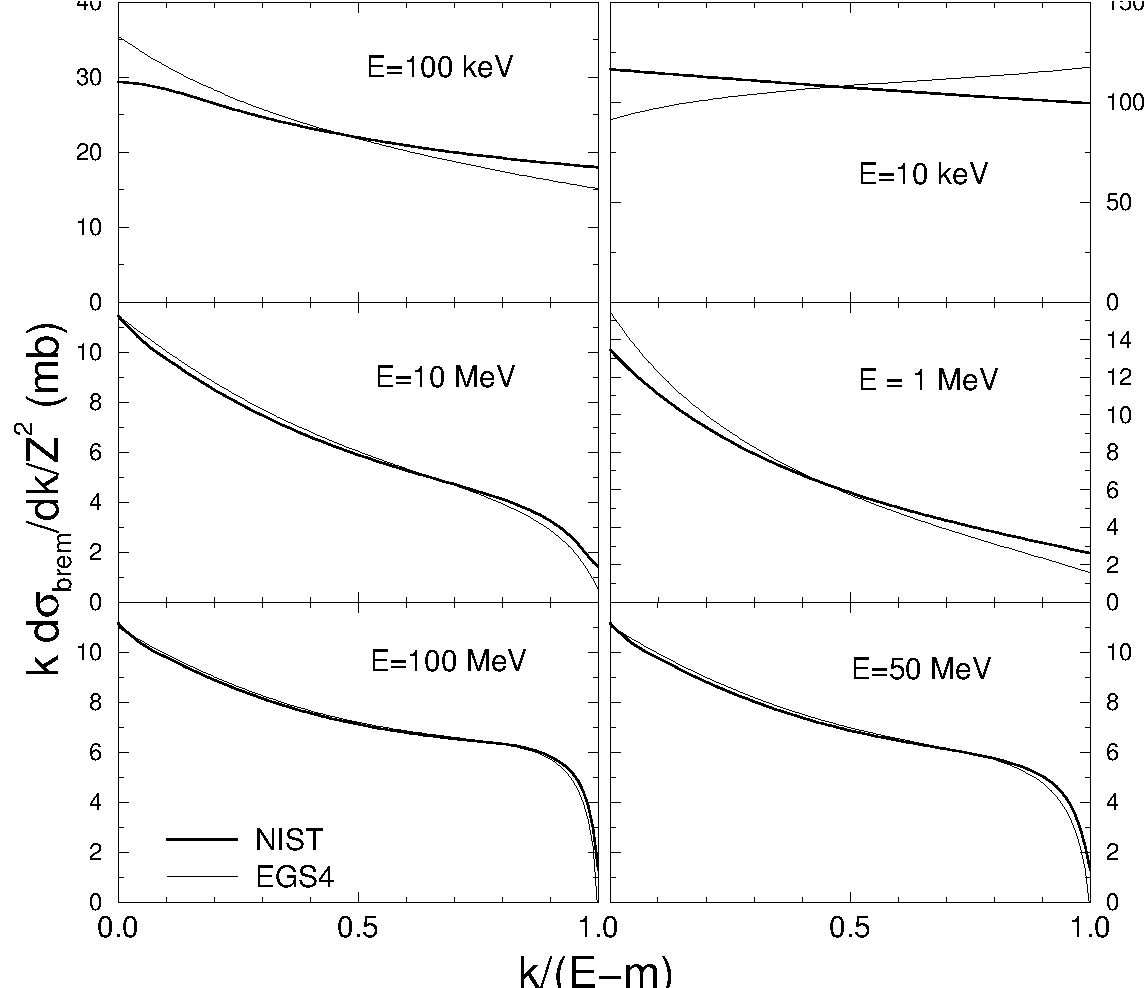
\includegraphics[height=15cm,width=15cm]{figures/brem79}
\caption[Bremsstrahlung cross sections]{\label{brems_fig1}
Differential bremsstrahlung cross sections
for gold at various incident electron energies from the NIST data base
\protect\cite{SB85,SB86a} (thick lines) compared to the
default EGSnrc (and EGS4) cross sections (thin lines). In both cases {\tt
IAPRIM = 1}, which is the default in the EGSnrc system and was an option
in the EGS4 system.}
\index{IAPRIM} \index{ibr\_nist}
\end{figure}
The behaviour for other materials is qualitatively similar.
As one can expect, the two cross sections are virtually
identical at high energies, but there are significant differences
at low energies (although the radiative stopping power is the
same due to the use of $A'$ from Eq. (\ref{brems_aprime})).

\paragraph{Simulation of discrete bremsstrahlung events, photon energy}
\hfill
\index{bremsstrahlung!simulation of}
\index{discrete interactions!bremsstrahlung}


In the course of the re-work of the EGS4 sampling routines
we have found an error in the sampling algorithm used in
EGS4. The error, which was most likely not discovered before
because it shows up only if the incident electron energy is
not much larger than the threshold energy $k_c$, is
demonstrated in Fig. \ref{brems_fig2}. This figure compares the distribution
sampled by the EGS4 routine {\tt BREMS} (points) for 100 keV
electrons in aluminum, expressed in
terms of $x$,
\begin{equation}
\label{brems_x}
x = {\ln k/k_c \over \ln T/k_c}~,
\end{equation}
to the theoretically expected result (solid line). The threshold
energy $k_c$ was 10 keV ($k_c$ is called {\tt AP} in EGS4 and EGSnrc).
%${\rm d}\sigma_{\rm brem}/{\rm d}x =
\begin{figure}[htp]
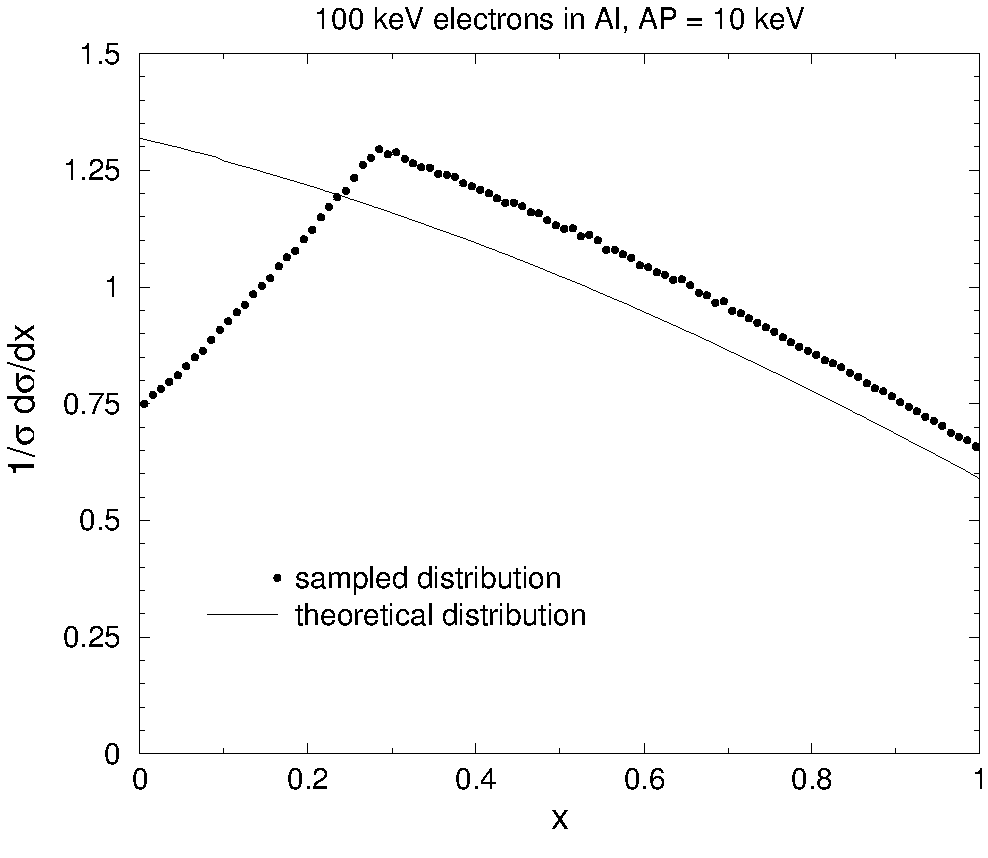
\includegraphics[height=12cm,width=12cm]{figures/Al_100keV}
\caption[{\tt BREMS} bug in EGS4]{\label{brems_fig2}
The distribution of photon energies
sampled by the EGS4 routine {\tt BREMS} (points) for 100 keV
electrons in aluminum, expressed in terms of $x$, defined in
Eq. (\protect\ref{brems_x}), compared to the theoretical
expectation.}
\end{figure}
This finding was a sufficient motivation to completely recode
the {\tt BREMS} routine.

The most efficient algorithm for sampling photon energies on
the basis of Eq. (\ref{brems_cs}) appears to be the following:
after a change of variables from $k$ to $x$, we have
\begin{eqnarray}
{{\rm d} \sigma_{\rm brem}(E,Z) \over {\rm d} x} & = & C
\left\{ \left(1 + {E^{' 2} \over E^2} \right)
\left[ \phi_1(\delta) - \frac{4}{3} \ln Z - 4 \tilde{f}_c(E,Z) \right]
\right. \nonumber \\ & - & \left.
\frac{2}{3}~\frac{E'}{E} \left[\phi_2(\delta) -
\frac{4}{3} \ln Z - 4 \tilde{f}_c(E,Z) \right]
\right\}
\end{eqnarray}
where $C$ is a constant combining factors irrelevant for
the sampling algorithm. Apart from a normalization
constant, the function in the curled brackets, to be denoted
in what follows with $R$, is the
quantity $k {\rm d}\sigma_{\tt brem}/{\rm d}k/Z^2$, shown
with the thin lines in Fig. \ref{brems_fig1}. As can be seen,
it is relatively flat and can therefore be employed as a
rejection function in conjunction with a uniform sampling
of $x$. $R$ retains its absolute maximum\footnote{The actual maximum
for a threshold energy
$k_c$ is slightly smaller and obtained for $k=k_c$, the difference between the
two is negligible except at low electron energies.}, $R_{\rm max}$, for
$k = 0$. It is given by
\begin{equation}
R_{\rm max} = 28.381 - \frac{4}{3} Z_V
\end{equation}
where $Z_V$ is defined in Eq. (\ref{pair_replace}) in section \ref{pair}
and we have made use of Eq. (\ref{pair_phi}) for the functions
$\phi_1(\delta)$ and $\phi_2(\delta)$.
The algorithm is then
\begin{enumerate}
\item
Calculate $b = \ln T/k_c$ \footnote{As the logarithm of the kinetic
energy is known prior to the call to the {\tt BREMS} routine
(because also used for other purposes), the time consuming
evaluation of the logarithm is not necessary if $\ln(k_c)$ is
stored in the computer memory for each medium.}
\item
Pick two random numbers, $r_1$ and $r_2$
\item
Set $k = k_c \exp(r_1 b)$, calculate $R/R_{\rm max}$
\item
If $r_2 > R/R_{\rm max}$, go to step 2
\item
Deliver $k$
\end{enumerate}
Figure \ref{brems_times} shows CPU times in $\mu$s necessary to sample one
photon energy on a 500 MHz PIII computer
using the new algorithm (solid line),
the EGS4 algorithm (dotted line) and using the alias sampling technique
in the case {\tt ibr\_nist} is set to 1.
\index{ibr\_nist}
\begin{figure}[htp]
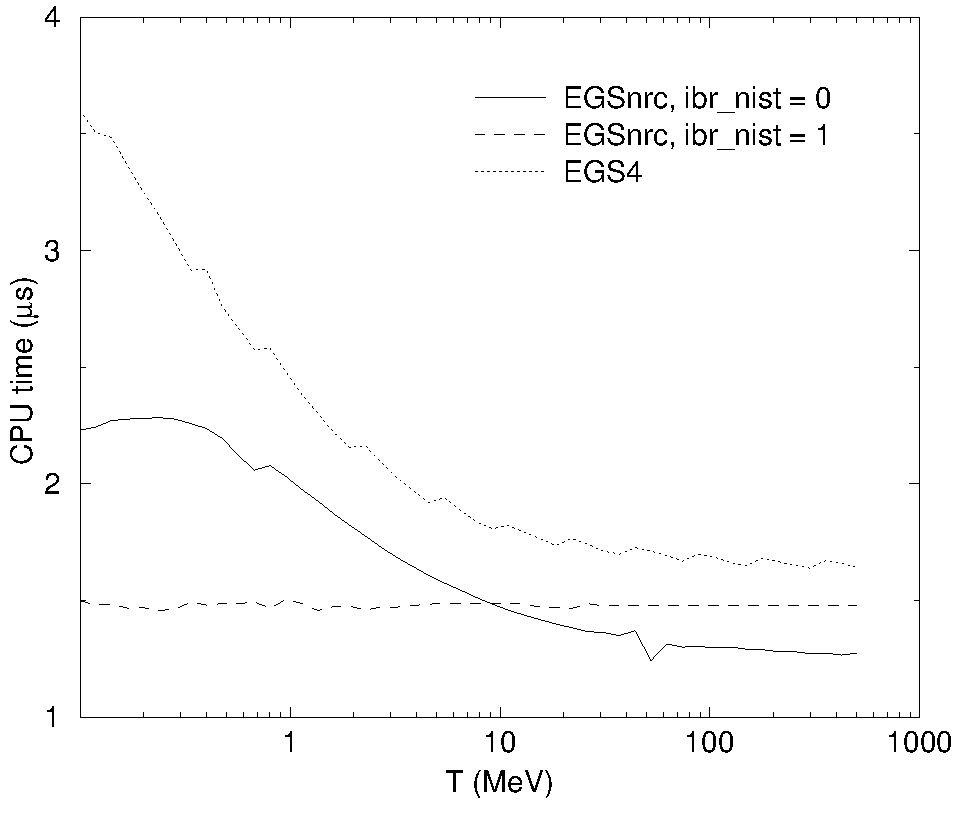
\includegraphics[height=12cm,width=12cm]{figures/brem_times}
\caption[CPU times for bremsstrahlung sampling]{\label{brems_times}
CPU times (in $\mu$s), as function of the incident electron kinetic
energy $T$, necessary to sample one photon energy using various
algorithms}
\end{figure}
The threshold energy used was $k_c = 10$~keV and the material
was aluminum. The precise
amount of CPU time spent for sampling the photon energy
is somewhat dependent on $k_c$ and $Z$, but the qualitative
behaviour remains the same for other values of $k_c$.
Apart from being more accurate, the new algorithm is also more
efficient. The CPU time for the alias sampling technique is
energy independent, as one can expect. It is faster at lower
energies but slower at high energies and so the use
of the {\tt ibr\_nist=1} option is not meaningful above 50 MeV
(where also the cross sections are identical). The small
``waves'' in the EGS4 curves are due to the technique employed
to sample the distribution $(1-\varepsilon)/\varepsilon$
(see the EGS4 manual, Ref \cite{Ne85}) which is at the same time
the reason for the error shown in Fig. \ref{brems_fig2}.
\index{SLAC-265}

\paragraph{Simulation of discrete bremsstrahlung events,
angular distribution}
\hfill
\index{bremsstrahlung!angular distribution}

In the original EGS4 implementation, the polar angle of bremsstrahlung
emission with respect to the initial electron direction was fixed
and given by $m/E$. In Ref. \cite{Bi89} an improved angle selection
scheme based on equation 2BS in the article by Koch and Motz \cite{KM59}
was implemented for use with EGS4. This implementation
was adopted in EGSnrc with slight modifications.
\index{Bielajew, Alex}

Equation 2BS, which is the bremsstrahlung cross section,
differential in the photon energy
$k$ and the photon emission angle $\theta$, is \cite{KM59}
\begin{eqnarray}
\label{brems_angle}
{\rm d}\sigma_{\rm brem}(k,\theta) & = & 4 \alpha Z^2 r_0^2 \frac{{\rm d}k}{k}
{y {\rm d} y \over (y^2 + 1)^2}
\left\{ {16 y^2 r \over (y^2 + 1)^2} - (1+r)^2 + \left[
1 + r^2 - {4 y^2 r \over (y^2 + 1)^2} \right] \ln M(y) \right\}
\nonumber \\
r & = & \frac{E'}{E}~, \quad y = \frac{E}{m} \theta~, \quad \frac{1}{M(y)} =
\Delta^2 + \left( {Z^{1/3} \over 111 (y^2 + 1)} \right)^2
\end{eqnarray}
where all definitions following Eq. (\ref{brems_cs}) apply.
Eq. (\ref{brems_angle}) is the result of an extreme relativistic,
first Born and small angle approximation, but it includes a
screening correction
based on a Thomas-Fermi potential. The effect of the screening
of the nucleus by atomic electrons is contained by the
expression in the brackets for $1/M(y)$. This can easily be
verified by comparing Eq. (\ref{brems_angle}) to equation
2BN(a) from the article by Koch and Motz which is derived
with the same approximations but using a bare nuclear potential.
In order to investigate the performance of
Eq. (\ref{brems_angle}) at low incident electron energies,
we can compare it to formula
2BN of the article by Koch and Motz which is for a bare
nucleus but does not involve the extreme relativistic
and small angle
approximations. For a ``fair'' comparison, screening corrections
must be negligible, this is the case if
\begin{equation}
\Delta^2 \gg \left( {Z^{1/3} \over 111 (y^2 + 1)} \right)^2 \quad
\mbox{or} \quad {k m \over E^2} \gg {2 Z^{2/3} \over 111^2}~,
\end{equation}
a condition which is satisfied in a wide range of photon/electron
energy combinations.
\begin{figure}[htp]
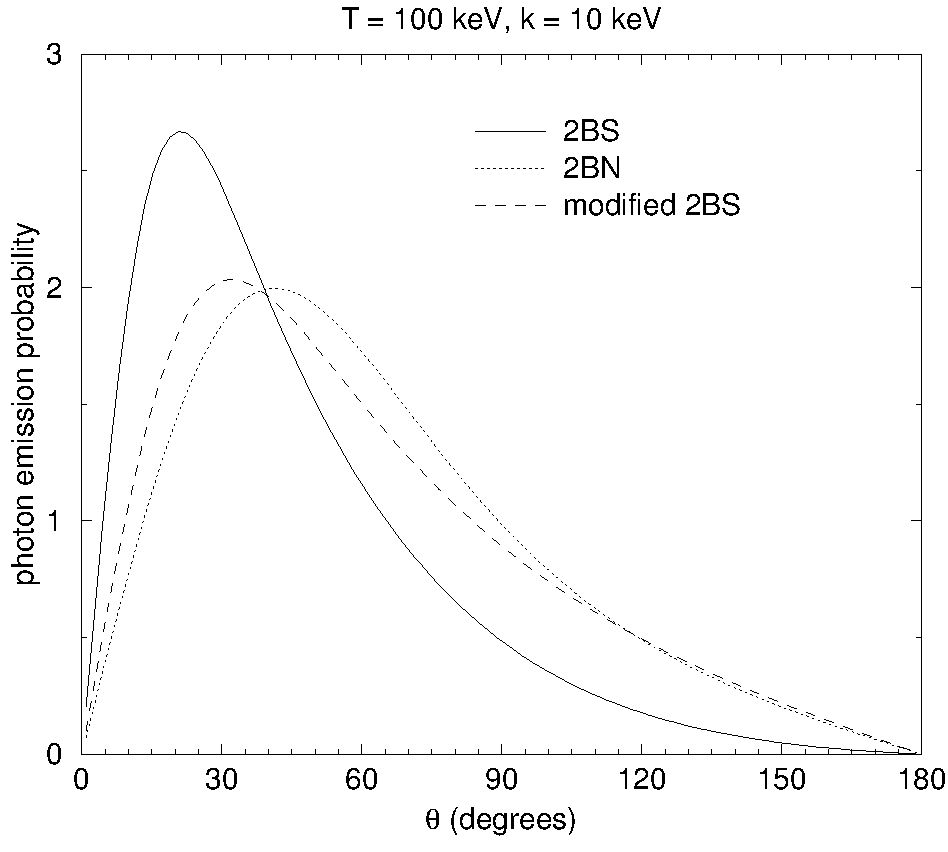
\includegraphics[height=12cm,width=12cm]{figures/bremang1}
\caption[Low energy bremsstrahlung angular distribution]{\label{brems_angle_fig1}
Angular distribution for emission of 10 keV bremsstrahlung photons
by 100 keV electrons in aluminum. Solid line represents
equation 2BS of Koch and Motz (Eq. (\ref{brems_angle}) in this
report), the dotted line equation 2BN of Koch and Motz, the
dashed line is 2BS with modifications as discussed in the text.}
\end{figure}
Figure \ref{brems_angle_fig1} shows a typical result of such
a comparison. The modification to 2BS that we have undertaken,
shown as a dashed line and obviously at a much better
agreement with formula 2BN,
is fairly simple and allows most of the considerations of
Ref.~\cite{Bi89} to be applied for the sampling procedure.
We note that the leading term of the distribution
2BN is $(1 - \beta \cos \theta)^{-2}$ where $\beta$ is the
electron velocity in units of the speed of light.
Approximated for
small angles and high energies it is equivalent to
the leading term of 2BS $(1 + y^2)^{-2}$, apart from a
normalization constant:
\index{Bielajew, Alex}
\begin{eqnarray}
(1 - \beta \cos \theta)^2 & \approx &
\left[1 - \beta\left(1 - \frac{\theta^2}{2}\right)\right]^2 =
(1 - \beta)^2 \left[ 1 + \theta^2 {\beta \over 1 - \beta} \right]^2
\nonumber \\
& = & (1 - \beta)^2 \left(1 + \beta (1 + \beta) \theta^2 \frac{E}{m} \right)^2
\approx (1 - \beta)^2 (1 + y^2)^2
\end{eqnarray}
We then use
\begin{equation}
y^2 = \beta (1 + \beta) \frac{E^2}{m^2} (1 - \cos \theta)
\end{equation}
in Eq. (\ref{brems_angle})\footnote{One could go one step
further and modify terms containing $y^2$ in the nominator
as they obviously come from expressions with $\sin^2 \theta$ but
this turns out to not improve the agreement to 2BN significantly}
and otherwise apply the results of
Ref. \cite{Bi89} so that the sampling algorithm is as follows:
\begin{enumerate}
\item
Calculate the maximum of the function in the curled brackets (to be
denoted by $f(y)$),
$f_{\rm max}$,
which is obtained for $y^2 = 0, y^2 = 1$ or $y^2 = y_{\rm max}^2 \equiv
2 \beta (1 + \beta) (E/m)^2$ for the current $E$ and $k$
\item
Pick two random numbers $r_1$ and $r_2$
\item
Sample $y^2$ from $y {\rm d}y/(1+y^2)^2$ using
\begin{equation}
y^2 = {r_1 y_{\rm max}^2 \over 1 + y_{\rm max}^2 (1 - r_1)}
\end{equation}
\item
If $r_2 > f(y)/f_{\rm max}$ go to step 2
\item
Deliver $\cos \theta$,
\begin{equation}
\cos \theta = 1 - {y^2 m^2 \over \beta (1 + \beta) E^2}
= 1 - \frac{y^2}{2 y_{\rm max}^2}
\end{equation}
\end{enumerate}
\index{IBRDST}
The efficiency of this algorithm is close to unity for low
energies and decreases logarithmically with increasing energy.
In addition, it requires several logarithm evaluations
(3 in step 1, 1 for each repetition of step 4) and is therefore
rather slow. We have therefore implemented a second bremsstrahlung
angle selection scheme which uses only the leading term of
the angular distribution and can be selected by the user
by setting the parameter {\tt IBRDST} in {\tt COMMON/BREMPR/} to zero
(the default {\tt IBRDST} value is 1,
{\em i.e.} modified 2BS from Koch and Motz).
We have found that the original
EGS4 fixed angle approach is not faster than using the
leading term of the angular distribution and have
therefore removed it.
\index{Bielajew, Alex}

\paragraph{Radiative splitting} \hfill
\label{rad_split}
\index{radiative splitting}
\index{bremsstrahlung!splitting}
\index{nbr\_split}
\index{variance reduction!brem splitting}

If the radiative splitting option is set ({\tt nbr\_split} $> 1$),
the result of a bremsstrahlung event will be {\tt nbr\_split}
photons, each having the fraction 1/{\tt nbr\_split} of
the weight of the electron, and an electron with an
energy given by its initial energy minus the energy of
the last bremsstrahlung photon produced. Note that
this violates energy conservation on an event-by-event
basis, energy is conserved only on average. The
motivation to ``inline'' the bremsstrahlung splitting technique
was that various quantities, necessary for the sampling
of photon energies, emission angles, and associated
rotations, can be calculated only once and then re-used
{\tt  nbr\_split} times.

It is worth noticing that if {\tt nbr\_split} is set
to zero, the bremsstrahlung event will be skipped.
This gives the possibility to study, for instance, the
influence of the neglect of bremsstrahlung production
on calculated quantities\footnote{A similar result
can be achieved by using {\tt IUNRST=4} when generating
the PEGS data but in this case the average energy lost to radiation
will be still subtracted and deposited locally.}, should
this be of any use to someone.

\subsubsection{Discrete inelastic collisions}
\label{discrete_inel}
\setcounter{equation}{0}
\index{inelastic collisions}
\index{binding effects}
\index{electron impact ionization}
\index{discrete interactions!inelastic collisions}

%At the present stage, binding effects are disregarded
%in the treatment of electron and positron inelastic
%scattering with atomic electrons in EGSnrc
%(and also in the default EGS4  version).
%Namito {\em et al} have implemented various
%electron impact ionization cross sections for
%use with EGS4 \cite{Na98}. We have studied their approach
%but decided to postpone the inclusion
%of binding effects until a more general treatment
%becomes available that can easily be applied
%to ``catastrophic'' {\em and} sub-threshold inelastic
%collisions.

When the binding of atomic electrons is ignored (default EGSnrc behavior),
electron-electron scattering can be described by the
M{\o}ller cross section \cite{Mo32a} and
positron-electron scattering by the Bhabha cross section
\cite{Bh35}. When binding is taken into account, interactions of
electrons and positrons with atoms can result in the creation of inner
shell vacancies, this process is usually referred to as electron impact
ionization (EII).

\paragraph{M{\o}ller scattering} \hfill
\index{M{\o}ller cross section}
\index{M{\o}ller scattering}
\index{discrete interactions!M{\o}ller scattering}
\index{cross section!M{\o}ller}

The M{\o}ller cross section, which is the cross section
for electron-electron scattering differential in the kinetic energy
$T'$ of the scattered electron which is initially at rest, is
\cite{ICRU37}
\begin{equation}
\label{moller_cs}
{{\rm d} \sigma_{\rm inel}^- \over  {\rm d}T'} =
{2 \pi r_0^2 m \over \beta^2}~\frac{1}{T^{\prime 2}} \left[
1 + {T^{' 2} \over (T - T')^2} + {\tau^2 \over (\tau+1)^2}~
\left(\frac{T'}{T}\right)^2
- {2 \tau + 1 \over (\tau + 1)^2}~{T' \over T - T'} \right]
\end{equation}
where $\beta$ is the incident electron velocity in units of the
speed of light, $T$ the incident kinetic energy and $\tau = T/m$.
Because the two electrons are indistinguishable, Eq. \eqref{moller_cs}
is symmetric with respect to exchange of the energies of the two scattered
particles. Per definition, the electron with the higher energy
after the collision is considered to be the primary, so that
the total cross section for M{\o}ller interactions is obtained
via integration of Eq. \eqref{moller_cs} from $T_c$ to $T/2$:
\begin{equation}
\label{moller_cs1}
\sigma_{\rm inel}^- = \int\limits_{T_c}^{T/2}
{{\rm d} \sigma_{\rm inel}^- \over  {\rm d}T'} {\rm d}T'
\end{equation}
\index{TE}
\index{AE}
In EGS4 and EGSnrc $T_c$ is called {\tt TE} and the corresponding
total energy {\tt AE}. The threshold kinetic energy above which M{\o}ller
events can occur is obviously $2 T_c$. The integration of
Eq. \eqref{moller_cs1} is trivial, and is evaluated by the
PEGS function {\tt AMOLTM}.
\index{AMOLTM}
\index{PEGS4!AMOLTM}

\index{M{\o}ller scattering!sampling of}
To sample the energy of the scattered electron on the basis of
Eq. \eqref{moller_cs}, one makes a change of variables to
$\varepsilon = T'/T$, which can take values between
$\varepsilon_0  = T_c/T$ and $1/2$, and after re-arranging
obtains \cite{Ne85}
\begin{equation}
\label{moller_cs2}
{{\rm d} \sigma_{\rm inel}^- \over  {\rm d} \varepsilon} =
C \left( {\varepsilon_0 \over 1 - 2 \varepsilon_0}~\frac{1}{\varepsilon^2}
\right) g(\varepsilon)
\end{equation}
where $C$ is a constant irrelevant for the sampling algorithm,
the expression in the brackets is a normalized PDF for $\varepsilon$
and $g(\varepsilon)$ will be used as a rejection function.
At this point it is worth noticing that there is an error in the EGS4 manual
for the rejection function $g(\varepsilon)$ and the resulting error
in the {\tt MOLLER} sampling routine was not
corrected in EGS4 until 1996 \cite{Bi96b}. The proper rejection function
reads
\index{SLAC-265}
\index{Bielajew, Alex}
\begin{equation}
\begin{split}
g(\varepsilon) &= {1 + g_2 \varepsilon^2 + r (r - g_3) \over
g_{\rm max} } \\ g_{\rm max} &= 1 + \frac{5}{4} g_2~, \quad
g_2 = {\tau^2 \over (\tau + 1)^2}~, \quad g_3 = {2 \tau + 1 \over (\tau+1)^2}~,
\quad r = {\varepsilon \over 1 - \varepsilon } ~.
\end{split}
\end{equation}
The algorithm used to sample $\varepsilon$ is then as follows:
\begin{enumerate}
\item
Calculate quantities dependent only on $T$, namely
\begin{displaymath}
\tau,~g_2,~g_3,~g_{\rm max}
\end{displaymath}
\item Pick two random numbers, $r_1$ and $r_2$
\item Sample $\varepsilon$ from the expression in the brackets in
Eq. \eqref{moller_cs2} using
\begin{equation}
\varepsilon = {T_c \over T - (T - 2 T_c) r_1}
\end{equation}
\item Calculate $g(\varepsilon)$, if $r_2 > g(\varepsilon)$  go to step 2
\item Deliver $\varepsilon$
\end{enumerate}
The efficiency of this algorithm is close to unity for
low incident energies $T$ but goes to $4/9$ at high energies.
A better approach would be the following: We can rewrite
Eq. \eqref{moller_cs1} as
\begin{equation}
\begin{split}
{{\rm d} \sigma_{\rm inel}^- \over  {\rm d}T'} & =
{2 \pi r_0^2 m \over \beta^2}~ \left[ F(T') + F(T-T') \right] \\
F(T') &= \frac{1}{T^{\prime 2}} + {1 \over 2 (T+m)^2} -
{2 \tau + 1 \over (\tau+1)^2}~\frac{1}{T T'} ~.
\end{split}
\end{equation}
If we now extend the range for $T'$ to $T-T_c$, we can drop
$F(T-T')$, and sample $T'$ from $F(T')$ only. At the end
$T'$ will be set to Min$(T',T-T')$. There are several possibilities
to sample $T'$ from $F(T')$. For instance, one can use
$1/T^{\prime 2}$ as a PDF and
\begin{equation}
g'(T') = \frac{1}{g'_{\rm max}} \left(1 + {T^{\prime 2} \over 2 (T+m)^2}
- {2 \tau + 1 \over (\tau + 1)^2}~ \frac{T'}{T} \right)
\end{equation}
as a rejection function. Here,
\begin{equation}
g_{\rm max} = \left\{
\begin{array}{r@{~~, \quad}l}
1 & \text{if}~~ \tau \le 2 + \sqrt{6} \\
{3 \tau^2 \over 2 (\tau+1)^2 } & \text{else}
\end{array} \right.
\end{equation}
The efficiency of such an algorithm is $2/3$ at high energies and
therefore 1.5 times better than the one used in EGS4 and EGSnrc.
Anticipating changes in the treatment of discrete inelastic
scattering, in order to take into account electron binding
effects, in the near future we have not implemented
this more efficient algorithm.

The polar scattering angles $\theta$ and $\theta'$
in M{\o}ller events are uniquely
determined by the kinematics. They are given by
\begin{equation}
\label{moller_angles}
\begin{split}
\cos \theta & = \sqrt{\frac{T-T'}{T}~\frac{T+2 m}{T-T' + 2 m}}~, \quad
\text{for the higher energy electron,} \\
\cos \theta' & = \sqrt{\frac{T'}{T}~\frac{T+2 m}{T' + 2 m}}~, \quad
\quad \quad \quad \quad  \text{for the lower energy electron.}
\end{split}
\end{equation}
The azimuthal angles are opposite and sample uniformly between
zero and $2 \pi$.

\paragraph{Bhabha scattering} \hfill
\index{Bhabha cross section}
\index{Bhabha scattering}
\index{discrete interactions!Bhabha scattering}
\index{cross section!Bhabha}

The Bhabha cross section, which is the cross section
for positron-electron scattering differential in the kinetic energy
$T'$ of the scattered electron which is initially at rest, is
given by \cite{Ne85}
\begin{equation}
\label{bhabha_cs}
{{\rm d} \sigma_{\rm inel}^+ \over  {\rm d}T'} =
{2 \pi r_0^2 m \over T^2} \left[ \frac{1}{\varepsilon}\left(
{1 \over \varepsilon \beta^2} - B_1 \right) + B_2 + \varepsilon
(\varepsilon B_4 - B_3 ) \right]
\end{equation}
where $T$ is the incident positron kinetic energy and
the following definitions apply:
\begin{equation}
\label{vhabha_cs1}
\begin{split}
\varepsilon & = \frac{T'}{T}, \quad \tau = \frac{T}{m},
\quad y = {1 \over \tau + 2}, \quad \beta^2 = {\tau (\tau + 2) \over
(\tau + 1)^2} \\
B_1 &= 2 - y^2, \quad B_2 = (1 - 2 y)(3 + y^2), \quad B_3 = B_4 +
(1 - 2 y)^2, \quad B_4 = (1 - 2 y)^3
\end{split}
\end{equation}
The range of possible $T'$ values is $T_c \cdots T$
({\em i.e.} the positron may have energy less then $T_c$
after Bhabha scattering).
The total discrete Bhabha cross section is then obtained
by integrating Eq. \eqref{bhabha_cs} in the allowed range,
{\em i.e.}
\begin{equation}
\sigma_{\rm inel}^+ = \int\limits_{T_c}^T {\rm d}T'
{{\rm d} \sigma_{\rm inel}^+ \over  {\rm d}T'}~.
\end{equation}
The integration is trivial but the result rather lengthy and therefore not
given here. The total discrete Bhabha cross section is evaluated
by the PEGS function {\tt BHABTM}.
\index{PEGS4!BHABTM}

\index{Bhabha scattering!sampling of}
The method employed to sample scattered electron energies on the basis
of Eq. \eqref{bhabha_cs} is similar to the M{\o}ller method.
The electron energy fraction $\varepsilon$ is sampled from
$1/\varepsilon^2$, the rejection function $g(\varepsilon)$ is
\begin{equation}
g(\varepsilon) = 1 - \beta^2 \varepsilon (B_1 - \varepsilon (B_2
- \varepsilon (B_3 - \varepsilon B_4)))~.
\end{equation}
As in the case of M{\o}ller scattering, there was an error for
the Bhabha scattering rejection function which was not corrected
until 1996 \cite{Bi96b}. Bhabha polar scattering angles are
given by Eq. \eqref{moller_angles}.
\index{Bielajew, Alex}

\subsubsection{Electron Impact Ionization}
\label{discrete_eii}
\setcounter{equation}{0}
\index{binding effects}
\index{electron impact ionization}
\index{discrete interactions!electron impact ionization}

Since 2003 the EGSnrc system has the ability to explicitely
simulate the creation of inner shell vacancies by electron or positron
impact for all K- and L-shells with binding energies above 1 keV.
This option can be turned on by setting the parameter {\tt eii\_flag} found
in {\tt COMIN/EII-DATA} to one. The differential cross sections used are
based on a semi-empirical theory described in Ref. \cite{Ka02b}. By default,
total EII cross sections are obtained by a numerical integration from these
differential cross sections. However, the user has the option to use
total EII cross sections from Gryzi\'{n}ski \cite{Gr65a}, Casnati \cite{Ca82}
Kolbenstvedt \cite{Ko67}, or Bote and Salvat \cite{BS08}.
This is accomplished by changing the parameter
{\tt eii\_xfile} found in {\tt COMIN/MEDIA} to {\tt gryzinski, casnati, kolbenstvedt} or {\tt penelope}. Users can also use their own
set of EII cross sections by setting
{\tt eii\_xfile} to an arbitrary charater string.
See section \ref{step_2} on page \pageref{eii_xfile_description}
for more detials.

When EII is turned on and there are K- or L-shells with
binding energies above {\tt AE} or {\tt AP} in the medium where a discrete
inelastic collision takes place, the probability for the collision being
with the K- or L-shell is computed. If a random number is less than this probability,
the interaction is simulated according to the EII differential cross sections of
Ref. \cite{Ka02b} and an inner shell vacancy is created that is subsequently relaxed
\index{relaxations}
using the subroutine {\tt RELAX} (see section \ref{relax}). Otherwise the
interaction is simulated according to the M{\o}ller or Bhabha cross sections.

\subsubsection{Two Photon Positron-Electron Annihilation}
\setcounter{equation}{0}
\label{annihilation}
\index{annihilation}
\index{positron annihilation}
\index{discrete interactions!annihilation}
\index{cross section!annihilation}

We have adopted the treatment
of the two photon positron annihilation process  from
EGS4 without modifications. For completeness
we give below the differential and total annihilation
cross sections as used in EGS4 and EGSnrc.

The cross
section, differential in the energy $k$ of the one
of the annihilation photons, for an incident positron with
a total energy of $E$ is \cite{Ne85}
\begin{equation}
\label{annih_cs}
{{\rm d} \sigma_{\rm annih} \over {\rm d} k} = {\pi r_0^2 \over \tau
(\tau+2)} \left[ S_1(\kappa) + S_1(\tau + 2 - \kappa) \right]
\end{equation}
where $\tau$ and $\kappa$ are the positron kinetic energy and photon
energy in units of $m$ and
\begin{equation}
S_1(x) = \frac{1}{x} \left( \tau + 2 + 2 {\tau + 1 \over \tau + 2} -
\frac{1}{x} \right) - 1~.
\end{equation}
Equation (\ref{annih_cs}) is obviously symmetric
under exchange of the annihilation photons,
the second photon has the energy $E + m - k$.

The polar emission angles of the annihilation photons are uniquely
determined by the kinematics and given by \cite{Ne85}
\begin{equation}
\label{annih_k_theta}
k = { m \over 1 - a \cos \theta}~,
\quad a = \sqrt{{\tau \over \tau + 2}}
\end{equation}
so that the minimum and maximum possible photon energies are
\begin{equation}
\label{annih_kminmax}
k_{\rm min} = {m \over 1 + a} ~, \quad
k_{\rm max} = {m \over 1 - a}~.
\end{equation}
The total annihilation cross section
is obtained by integrating Eq. (\ref{annih_cs})
over the allowed $k$-range and can be written as
\begin{equation}
\sigma_{\rm annih} = {\pi r_0^2 \over \tau + 2} \left[
{\tau^2 + 6 \tau + 6 \over \tau (\tau + 2)} \ln\left(\tau + 1
+ \sqrt{\tau (\tau + 2)} \right) - {\tau + 4 \over \sqrt{\tau (\tau + 2)}}
\right]
\end{equation}
At high energies ($\tau \gg 1$) $\sigma_{\rm annih}$
decreases as $(\ln \tau)/\tau$, for $\tau \to 0$ the cross section
tends to infinity ({\em i.e.} positrons always annihilate at rest
if they have not annihilated before).

The annihilation process is a ``catastrophic'' event and
treated discretely.

\index{annihilation!sampling of}
To sample the energy of one of the photons from
Eq. (\ref{annih_cs}), one makes a change in variables
to $\varepsilon = \kappa/(\tau+2)$, drops the second
$S_1$ because of the symmetry, and after re-arranging obtains
\begin{eqnarray}
{{\rm d} \sigma_{\rm annih} \over {\rm d}\varepsilon} & = &
C f(\varepsilon) g(\varepsilon) \\
f(\varepsilon) & = & {1 \over \ln[(1-\varepsilon_0)/\varepsilon_0]}~
\frac{1}{\varepsilon}~, \quad
%g(\varepsilon) = 1 - \varepsilon + {2 (\tau + 1) \varepsilon - 1 \over
%(\tau + 2)^2 }
g(\varepsilon) = 1 - {[\varepsilon (\tau+2) - 1) ]^2 \over \varepsilon
(\tau^2 + 4 \tau + 2) }
\end{eqnarray}
where $C$ is a constant that contains factors irrelevant for
the sampling procedure and $\varepsilon_0$ the minimum
possible value for $\varepsilon$,
\begin{equation}
\varepsilon_0 = {1 \over (\tau+2) (1 + a)}~.
\end{equation}
The function $f(\varepsilon)$ is a normalized PDF, $g(\varepsilon)$
is always positive and
has a maximum
of $1$ for $\epsilon = 1/(\tau+2)$ and
thus is a valid rejection function\footnote{Note that our $g(\varepsilon)$ is
the $g(\varepsilon)$ defined in Eq (2.12.26) of the EGS4 manual
divided by its maximum.}. The sampling algorithm is then as follows:
\begin{enumerate}
\item
Compute quantities dependent on $E$, namely
\begin{displaymath}
\tau,~A = \tau+2,~a,~\varepsilon_0,~
b = \ln{1 - \varepsilon_0 \over \varepsilon_0}
\end{displaymath}
\item
Pick two random numbers, $r_1$ and $r_2$
\item
Set
\begin{equation}
\varepsilon = \varepsilon_0 \exp\left(r_1 b\right)
\end{equation}
and calculate $g(\varepsilon)$
\item
If $r_2 > g(\varepsilon)$, the go to step 2
\item
Deliver $\varepsilon$
\end{enumerate}

\index{annihilation!single photon}
\index{annihilation!three photon}
At this point
one should perhaps mention that a single photon or three or more
photon annihilation processes in the nuclear field are also
possible. Messel and Crawford \cite{MC70} point out that
the ratio of one to two photon annihilation cross sections is small
until higher energies are reached, at which point the absolute
value of the cross section is small. Thus, the single
photon annihilation process is ignored. Positron annihilation to
three or more photons is even less likely than one photon
annihilation and therefore also ignored.

\index{annihilation!at rest}
If positrons do not annihilate in flight, they
annihilate at rest producing two photons. As one can easily
verify from Eq. \eqref{annih_k_theta} and \eqref{annih_kminmax},
the photon energies go to $m$ as $\tau$ goes to zero.
In addition, the cross section differential in the
photon emission angle becomes uniform in the limit $\tau \to 0$.

\index{radiative splitting}
\index{variance reduction!radiative splitting}
\index{nbr\_split}
If radiative splitting is set ({\tt nbr\_split} $> 1$),
the annihilation process will produce 2 {\tt nbr\_split} photons,
each carrying the fraction 1/{\tt nbr\_split} from the positron weight.
Simultaneous production of {\tt nbr\_split} annihilation
events allows the quantity $b$ (see step 1) as well as
parameter related to angular rotations to be re-used
{\tt nbr\_split} times.

\subsubsection{Collision stopping power}
\label{stopping_power}
\setcounter{equation}{0}
\index{stopping powers}
\index{restricted stopping powers}
\index{collision stopping powers}

\index{Seltzer, Stephen}
\index{Berger, Martin}
EGSnrc ``inherits'' the treatment of restricted collision
stopping powers from EGS4, {\em i.e.} uses the formulas
recommended by Seltzer and Berger \cite{BS64} which are based
on the Bethe-Bloch theory \cite{Be30,Be32,Bl33}. The standard
treatment (see also ICRU report 37 \cite{ICRU37} which was
used as the source of the formulas below)
assumes that there is a certain value for energy
transfer to atomic electrons, $T_{\rm med}$, that is (i)
large compared to the binding energies (ii) corresponds to
an impact parameter that is large compared to the atomic
dimensions. Collision processes that are associated with
energy loss $T'$ less than $T_{\rm med}$ are treated according to
the theory of Bethe, the main result of which is that
\begin{equation}
L_{\rm coll}^\pm(T,T' < T_{\rm med}) = {2 \pi r_0^2 m n \over \beta^2}
\left[ \ln \left(2 m \beta^2 T_{\rm med} \over (1 - \beta^2) I^2 \right)
- \beta^2 - \delta \right]
\end{equation}
where $\beta$ is again the electron velocity in units of
the speed of light, $I$ is the mean ionization energy and
$\delta$ the density effect correction that takes into
\index{density effect}
account the polarization of the medium due to the electron field.
As $T_{\rm med}$ is defined being large compared to the binding energies of
the atom, collision processes with energy transfer larger
than $T_{\rm med}$ can be treated using the M{\o}ller \cite{Mo32a} (electrons)
or Bhabha \cite{Bh35} (positron) cross section (see also section
\ref{discrete_inel}), {\em i.e.}
\index{$T_{\rm med}$}
\index{M{\o}ller cross section} \index{Bhabha cross section}
\begin{equation}
L_{\rm coll}^\pm(T,T' > T_{\rm med}) = \int\limits_{T_{\rm med}}^{T_c}
{\rm d}T' T' {{\rm d} \sigma_{\rm inel}^\pm \over {\rm d}T'}
\end{equation}
Using some additional approximations, $T_{\rm med}$ drops out
in the sum of $L_{\rm coll}^\pm(E,T' < T_{\rm med})$ and
$L_{\rm coll}^\pm(E,T' > T_{\rm med})$ and one obtains
\begin{equation}
L_{\rm coll}^\pm(T,T_c) = {2 \pi r_0^2 m n \over \beta^2}
\left[ \ln {T^2 \over I^2} + \ln(1 + \tau/2) + G^\pm(\tau) - \delta \right]
\end{equation}
where $\tau = T/m$ and the functions $G^\pm$ are different for
electrons and positrons due to differences in the M{\o}ller and
Bhabha cross sections and are given by
\index{Bhabha scattering}
\begin{equation}
\begin{split}
G^-(\tau) & = -1 - \beta^2  + \ln\left[4 \eta (1 - \eta) \right] +
{1 \over 1 - \eta} + (1 - \beta^2) \left[ {\tau^2 \eta^2 \over 2} +
(2 \tau + 1) \ln(1 - \eta) \right] \\
G^+(\tau) & = \ln(4 \eta) - \beta^2 \left[ 1 + (2 - y^2) \eta -
(3 + y^2) {y \tau \over 2} \eta^2 + (1 + y \tau) {y^2 \tau^2 \over 3} \eta^3
- {y^3 \tau^3 \over 4} \eta^4
\right]
\end{split}
\end{equation}
where $\eta = T_c/T$ and $y$ is defined in Eq. \eqref{bhabha_cs}.

\index{Class II scheme!validity of}
From the above discussion and from the general discussion
of a Class II condensed history implementation in section
\ref{electron_general} it is clear that the formalism
used to treat inelastic collisions with atomic electrons
is only applicable if
\begin{equation}
\label{Tc_condition}
T_c \gg ~~\text{binding energies of the medium of interest}.
\end{equation}
This imposes a rather severe limitation on the use
of Class II condensed history codes in high-$Z$ materials
(the $K$-shell binding energy for lead is, for instance, 88 keV).
We are therefore currently investigating a more realistic approach for
situations when the condition \eqref{Tc_condition} is not
satisfied, but its implementation into EGSnrc is left for the
next release of the system. One should probably also mention
that the many successful studies carried out with the
EGS4 system indicate that the implications of violating
the requirement \eqref{Tc_condition} are perhaps less
severe than one might expect from purely theoretical arguments.

\index{mean ionization energy}
\index{density effect}
\index{stopping powers}
The only non-trivial parameters of the restricted stopping
power formula are the mean ionization energy $I$ and the
density effect correction $\delta$. The default mean ionization
energies for elements used in PEGS4, along with atomic numbers,
weights, chemical symbols, and mass densities are summarized
in Table \ref{I_values}. Mean ionization energies for
compounds are derived from
\begin{equation}
\ln I = \sum p_i Z_i \ln I(Z_i)
\end{equation}
where $p_i$ is the stoichiometric index of the $i$'th element
which has atomic number $Z_i$ and a mean ionization energy $I(Z_i)$,
unless the material belongs to a set of pre-defined materials
to be found in Table 2.13.2 of the EGS4 manual \cite{Ne85} or listed in the
{\tt BLOCK DATA} section of {\tt pegs4.mortran}.
\index{pegs4.mortran}
\index{SLAC-265}

\index{Seltzer, Stephen}
\index{Berger, Martin}
\index{ISSB}
The density effects correction
has been treated extensively in the literature.
The default PEGS4 approach is based on the formulation of Sternheimer and
Peierls\cite{SP71} which basically parameterizes the density effect in
terms of 6 parameters ({\tt AFACT, SK, X0, X1, CBAR}, and {\tt IEV}).  This same parameterized approach was used for
the calculations by Berger and Seltzer \cite{BS83} and by
Sternheimer, Berger and  Seltzer \cite{St82} who fitted the parameters to
the density effect as calculated for the ICRU for increasingly larger
numbers of materials.  The power of PEGS4 is that it will generate a
density effect for any arbitrary material, if need be with no recourse to the fitted
parameters. In this case it will use the  Sternheimer and
Peierls\cite{SP71} general formula.  There is also an option in PEGS4 which allows the 6
parameters to be read in directly (using the {\tt ISSB=1} option in PEGS4,
see section~\ref{issb} page~\pageref{issb}). However, these
parameterizations are only fits to the actual density effect data. An
option was added to PEGS4 in 1989 which allowed the density effect data
to be used directly\cite{Du89} and the EGSnrc distribution includes a huge
data base of all the density effect values calculated by Seltzer and Berger
for ICRU Report 37\cite{ICRU37}.
To turn this option on the user must
set the flag {\tt EPSTFL} to 1 in the PEGS4 input file. See
section~\ref{icru37_csp} (page~\pageref{icru37_csp}) for more details.
In this case the density effect correction is calculated
by interpolation from pre-computed values stored in
a separate file.
Selecting this option has the additional effect that the mean
ionization energy of the material is taken directly from
the density effect correction file. It should be noted that in general the
differences in collision stopping powers between using the default Sternheimer
and Peierls density effect, or the fitted parameters or the direct ICRU 37
values, are small, of the order of a few percent at most.  These
differences are only
likely of importance for very detailed work.
\index{density effect}
\index{PEGS4!EPSTFL}
\index{EPSTFL}

\begin{longtable}{|rcrrr|}
\caption{\label{I_values}Default atomic numbers, symbols, atomic weights,
mass densities, and I values for elements in PEGS4.} \\
\hline \hline
 Z & Symbol & Atomic & Density & I(eV) \\
   &        & weight & (g/cm$^3$) &  \\
\hline
\endfirsthead
\hline
\multicolumn{5}{r}%
  {\small\slshape continued from previous page} \\
\hline \hline
 Z & Symbol & Atomic & Density & I(eV) \\
   &        & weight & (g/cm$^3$) & \\
\hline
\endhead
\hline
\multicolumn{5}{r}%
  {\small\slshape continued on next page} \\ \hline
\endfoot
\hline \hline
\endlastfoot
 1 & H      &  1.00797 &  0.0808    & 19.2 \\
 2 & HE     &  4.00260 &  0.1900    & 41.8 \\
 3 & LI     &  6.93900 &  0.5340    & 40.0 \\
 4 & BE     &  9.01220 &  1.8500    & 63.7 \\
 5 & B      & 10.81100 &  2.5000    & 76.0 \\
 6 & C      & 12.01115 &  2.2600    & 78.0 \\
 7 & N      & 14.00670 &  1.1400    & 82.0 \\
 8 & O      & 15.99940 &  1.5680    & 95.0 \\
 9 & F      & 18.99840 &  1.5000    &115.0 \\
10 & NE     & 20.18300 &  1.0000    &137.0 \\
11 & NA     & 22.98980 &  0.9712    &149.0 \\
12 & MG     & 24.31200 &  1.7400    &156.0 \\
13 & AL     & 26.98150 &  2.7020    &166.0 \\
14 & SI     & 28.08800 &  2.4000    &173.0 \\
15 & P      & 30.97380 &  1.8200    &173.0 \\
16 & S      & 32.06400 &  2.0700    &180.0 \\
17 & CL     & 35.45300 &  2.2000    &174.0 \\
18 & AR     & 39.94800 &  1.6500    &188.0 \\
19 & K      & 39.10200 &  0.8600    &190.0 \\
20 & CA     & 40.08000 &  1.5500    &191.0 \\
21 & SC     & 44.95600 &  3.0200    &216.0 \\
22 & TI     & 47.90000 &  4.5400    &233.0 \\
23 & V      & 50.94200 &  5.8700    &245.0 \\
24 & CR     & 51.99800 &  7.1400    &257.0 \\
25 & MN     & 54.93800 &  7.3000    &272.0 \\
26 & FE     & 55.84700 &  7.8600    &286.0 \\
27 & CO     & 58.93320 &  8.7100    &297.0 \\
28 & NI     & 58.71000 &  8.9000    &311.0 \\
29 & CU     & 63.54000 &  8.9333    &322.0 \\
30 & ZN     & 65.37000 &  7.1400    &330.0 \\
31 & GA     & 69.72000 &  5.9100    &334.0 \\
32 & GE     & 72.59000 &  5.3600    &350.0 \\
33 & AS     & 74.92160 &  5.7300    &347.0 \\
34 & SE     & 78.96000 &  4.8000    &348.0 \\
35 & BR     & 79.80800 &  4.2000    &357.0 \\
36 & KR     & 83.80000 &  3.4000    &352.0 \\
37 & RB     & 85.47000 &  1.5300    &363.0 \\
38 & SR     & 87.62000 &  2.6000    &366.0 \\
39 & Y      & 88.90500 &  4.4700    &379.0 \\
40 & ZR     & 91.22000 &  6.4000    &393.0 \\
41 & NB     & 92.90600 &  8.5700    &417.0 \\
42 & MO     & 95.94000 &  9.0100    &424.0 \\
43 & TC     & 99.00000 & 11.5000    &428.0 \\
44 & RU     &101.07000 & 12.2000    &441.0 \\
45 & RH     &102.90500 & 12.5000    &449.0 \\
46 & PD     &106.40000 & 12.0000    &470.0 \\
47 & AG     &107.87000 & 10.5000    &470.0 \\
48 & CD     &112.40000 &  8.6500    &469.0 \\
49 & IN     &114.82000 &  7.3000    &488.0 \\
50 & SN     &118.69000 &  7.3100    &488.0 \\
51 & SB     &121.75000 &  6.6840    &487.0 \\
52 & TE     &127.60000 &  6.2400    &485.0 \\
53 & I      &126.90440 &  4.9300    &491.0 \\
54 & XE     &131.30000 &  2.7000    &482.0 \\
55 & CS     &132.90500 &  1.8730    &488.0 \\
56 & BA     &137.34000 &  3.5000    &491.0 \\
57 & LA     &138.91000 &  6.1500    &501.0 \\
58 & CE     &140.12000 &  6.9000    &523.0 \\
59 & PR     &140.90700 &  6.7690    &535.0 \\
60 & ND     &144.24001 &  7.0070    &546.0 \\
61 & PM     &147.00000 &  1.0000    &560.0 \\
62 & SM     &150.35001 &  7.5400    &574.0 \\
63 & EU     &151.98000 &  5.1700    &580.0 \\
64 & GD     &157.25000 &  7.8700    &591.0 \\
65 & TB     &158.92400 &  8.2500    &614.0 \\
66 & DY     &162.50000 &  8.5600    &628.0 \\
67 & HO     &164.92999 &  8.8000    &650.0 \\
68 & ER     &167.25999 &  9.0600    &658.0 \\
69 & TM     &168.93401 &  9.3200    &674.0 \\
70 & YB     &173.03999 &  6.9600    &684.0 \\
71 & LU     &174.97000 &  9.8500    &694.0 \\
72 & HF     &178.49001 & 11.4000    &705.0 \\
73 & TA     &180.94800 & 16.6000    &718.0 \\
74 & W      &183.85001 & 19.3000    &727.0 \\
75 & RE     &186.20000 & 20.5300    &736.0 \\
76 & OS     &190.20000 & 22.4800    &746.0 \\
77 & IR     &192.20000 & 22.4200    &757.0 \\
78 & PT     &195.08000 & 21.4500    &790.0 \\
79 & AU     &196.98700 & 19.3000    &790.0 \\
80 & HG     &200.59000 & 14.1900    &800.0 \\
81 & TL     &204.37000 & 11.8500    &810.0 \\
82 & PB     &207.19000 & 11.3400    &823.0 \\
83 & BI     &208.98000 &  9.7800    &823.0 \\
84 & PO     &210.00000 &  9.3000    &830.0 \\
85 & AT     &210.00000 &  1.0000    &825.0 \\
86 & RN     &222.00000 &  4.0000    &794.0 \\
87 & FR     &223.00000 &  1.0000    &827.0 \\
88 & RA     &226.00000 &  5.0000    &826.0 \\
89 & AC     &227.00000 &  1.0000    &841.0 \\
90 & TH     &232.03600 & 11.0000    &847.0 \\
91 & PA     &231.00000 & 15.3700    &878.0 \\
92 & U      &238.03000 & 18.9000    &890.0 \\
93 & NP     &237.00000 & 20.5000    &902.0 \\
94 & PU     &242.00000 & 19.7370    &921.0 \\
95 & AM     &243.00000 & 11.7000    &934.0 \\
96 & CM     &247.00000 &  7.0000    &939.0 \\
97 & BK     &247.00000 &  1.0000    &952.0 \\
98 & CF     &248.00000 &  1.0000    &966.0 \\
99 & ES     &254.00000 &  1.0000    &980.0 \\
100& FM     &253.00000 &  1.0000    &994.0 \\
%\hline \hline
%\end{tabular}
%\end{center}
%\end{supertabular}
%\end{table}
\end{longtable}

\subsubsection{Elastic scattering cross sections}
\label{elastic}
\setcounter{equation}{0}
\index{elastic scattering}
\index{spin effects}
\index{cross section!elastic}

\index{SPIN\_EFFECTS}
The treatment of electron and positron elastic
scattering in EGSnrc is determined by the logical parameter
{\tt SPIN\_EFFECTS} which is in {\tt common/ET\_Control/}.
If set to {\tt .true.} (this is the default),
elastic scattering cross sections
that take into account spin effects are employed, they
are discussed in section \ref{spin_elastic}. If {\tt .false.},
elastic scattering is based on the screened Rutherford cross section.
This is consistent with EGS4, although multiple elastic
\index{multiple elastic scattering}
\index{\Mol~theory}
scattering (see section \ref{sec_MS})
is based on an exact theory rather than the
small-angle theory of \Mol \cite{Mo48} which is used in EGS4.
\index{screened Rutherford cross section}

\paragraph{Screened Rutherford elastic scattering} \hfill
\index{screened Rutherford cross section}

The screened Rutherford cross section, which is the cross
section differential in the cosine $\mu$ of the polar
scattering angle of electrons or positrons incident
on atoms of atomic number $Z$, is
\begin{equation}
\label{SR_1}
{{\rm d} \sigma_{\rm SR} \over {\rm d}\mu} = {2 \pi r_0^2 Z^2 \over
\beta^2 \tau (\tau + 2) }~{1 \over (1 - \mu + 2 \eta)^2}
\end{equation}
where $\beta$ is the particle velocity in units of the speed of
light, $\tau$ the kinetic energy $T$ in units of $m$
\index{screening parameter}
and $\eta$ the screening parameter. The total elastic scattering
cross section is obtained from Eq. \eqref{SR_1} by integrating
over $\mu$ from -1 to 1 and is given by
\begin{equation}
\label{SR_2}
\sigma_{\rm SR} = {\pi r_0^2 Z^2 \over \beta^2 \tau (\tau+2) \eta (1 + \eta)}
\end{equation}
In EGS4 the screening parameter $\eta$ is based on the single
elastic scattering theory of \Mol \cite{Mo47}. \Mol~
\index{PWA}
performed a partial-wave analysis (PWA) expansion
of the Klein-Gordon equation ({\em i.e.} he neglected spin effects)
in the nuclear field described by the Thomas-Fermi potential,
used a small-angle approximation ({\em i.e.} replaced the Legendre
Polynomials by zeroth order Bessel functions $J_0$),
and employed a WKB-expansion
of the resulting radial equation up to zeroth order in $\hbar$
to calculate the phase shifts $\phi(z)$ to arrive at
\begin{equation}
\label{el_mol}
{{\rm d} \sigma_{\rm M} \over \chi {\rm d} \chi} =
2 \pi a^2 \left| \int\limits_0^\infty {\rm d}z z J_0\left(z {\chi \over
2 \sqrt{\eta_0}} \right) \left[ \exp\Big( - 2 i \alpha'
\phi(z) \Big) - 1 \right]
\right|^2
\end{equation}
where $\chi$ is the scattering angle, $a$ is the Thomas-Fermi radius,
$\eta_0$ is defined in Eq. \eqref{eta_0} and $\alpha'$ given by
\begin{equation}
\label{alpha_prime}
\alpha' = {\alpha Z \over \beta}
\end{equation}
($\alpha \approx 1/137$ is the fine structure constant). In addition
he approximated the Thomas-Fermi potential by the sum of three
exponential functions in which case the phase shifts $\phi(z)$ are
given by zeroth order modified Bessel functions. He then required
that the average scattering angle squared, calculated from a
screened Rutherford cross section is the same as the average
scattering angle squared resulting from Eq. \eqref{el_mol} and,
after studying the limiting cases $\alpha' \to 0$ and
$\alpha' \to \infty$, arrived at the simple formula
\begin{equation}
\label{eta_0}
\eta = \eta_0 (1.13 + 3.76 \alpha^{\prime 2} )~, \quad
\eta_0 = {\alpha^2 Z^{2/3} \over 4 C_{\rm TF}^2 \tau (\tau + 2)}~,
\quad C_{\rm TF} = \left( {9 \pi^2 \over 128} \right)^{1/3}
\end{equation}
for the effective screening parameter $\eta$\footnote{Note that our
$\eta$ is \Mol's $\chi_a^2/4$, $C_{\rm TF}$ is the Thomas-Fermi
constant.}.

The treatment of elastic scattering in EGS4 is intrinsically
associated with \Mol's multiple scattering theory\cite{Mo48}.
In his treatment of multiple scattering \Mol~ uses a small-angle
approximation in which case the moments of the screened Rutherford
cross section (see section \ref{sec_MS}) are given by
first order modified Bessel functions $K_1$.
%{\em i.e.}
%\begin{equation}
%\int\limits_{-1}^1 {\rm d} \mu \Big[1 - P_l(\mu) \Big]
%{{\rm d}
In addition, a small argument expansion of $K_1$ is performed
so that the elastic scattering cross section for
compounds and mixtures can be expressed with two
parameters, $b_c$ and $\chi_{cc}$, as follows:
\begin{equation}
\begin{split}
b_c & =  {4 \pi r_0^2 C_{\rm TF}^2 \rho \over 1.13 \alpha^2 u}
{Z_S \exp(Z_E/Z_S) \over A \exp(Z_X/Z_S)} = 7821.6~ \mbox{cm}^2/\mbox{g}~\rho
{ Z_S \exp(Z_E/Z_S) \over A \exp(Z_X/Z_S)} \\
\chi_{cc}^2 & = {4 \pi r_0^2 m^2 \over u}~\rho~\frac{Z_S}{A} = 0.1569~
\mbox{cm}^2 \mbox{MeV}^2 / \mbox{g}~\rho \frac{Z_S}{A}
\end{split}
\end{equation}
where $A$ is the relative molecular mass and
\begin{equation}
\begin{split}
Z_S & = \sum p_i Z_i (Z_i + \xi_{\rm MS} ) \\
Z_E & = \sum p_i Z_i (Z_i + \xi_{\rm MS} ) \ln Z_i^{-2/3} \\
Z_X & = \sum p_i Z_i (Z_i + \xi_{\rm MS} ) \ln \left(1 + 3.34~ \alpha^2 Z_i^2
\right)
\end{split}
\end{equation}
\index{angular deflections!inelastic collisions}
Note that in the expression for $Z_X$ $\alpha'$ was replaced
by $\alpha Z_i$ and we have removed the factor 1.167 in the
denominator of the expression for $b_c$ in the EGS4 manual,
this factor is not necessary when multiple scattering is
treated with the exact formulation. The purpose of the
parameter $\xi_{\rm MS}$ is to take into account
contributions from sub-threshold inelastic scattering
with atomic electrons. In PEGS4 a macros {\tt \$FUDGEMS} is
used for $\xi_{\rm MS}$ with the intent to provide
the user with the possibility of implementing a more
realistic treatment of sub-threshold inelastic
contributions. Experience shows that
this capability is rarely used and so, PEGS4 generated
data sets usually have $\xi_{\rm MS}=1$ (the default value).
This leads to double counting of angular deflections due
to sub-threshold inelastic collisions (see {\em e.g.} \cite{LR94a}).
This problem remains present in EGSnrc if the screened
Rutherford cross section is used to model elastic collisions
(parameter {\tt SPIN\_EFFECTS} is set to {\tt .false.}).
We have not attempted a correction in this case as the neglect of spin
effects represents a more severe approximation than the
double counting of inelastic collisions. A more
realistic approach is used when spin effects are turned on,
see next section.
\index{SPIN\_EFFECTS}
\index{\$FUDGEMS}
\index{PEGS4!\$FUDGEMS}

%\index{{\tt BLCC}}
%\index{{\tt XCC}}
\index{BLCC}
\index{XCC}
In terms of the parameter $b_c$ and $\chi_{cc}$,
which are called {\tt BLCC} and {\tt XCC},
the screening parameter is
\begin{equation}
\label{calc_eta}
\eta = {\chi_{cc}^2 \over 4 b_c m^2 \tau (\tau + 2)}
\end{equation}
and the total macroscopic cross section
\begin{equation}
\label{SR_tot}
\Sigma_{\rm SR} = {b_c \over \beta^2}
\end{equation}
The latter formula involves the neglect of $1 + \eta$ in the denominator
of Eq. \eqref{SR_2}.

\index{angular deflections!single elastic scattering}
\index{single elastic scattering}
Sampling angular deflections in single elastic scattering events
on the basis of Eq. \eqref{SR_1} is trivial, it is accomplished by
\begin{equation}
\label{sample_SR}
\mu = 1 - {2 \eta r \over 1 - r + \eta}
\end{equation}
where $r$ denotes a random number between zero and unity.
Single elastic scattering deflections are necessary when
boundary crossing between different media is modelled exactly,
see section \ref{BCA}.

\paragraph{Elastic scattering with spin} \hfill
\label{spin_elastic}
\index{spin effects}
\index{PWA}
\index{elastic scattering!spin effects}

Potentially the most accurate elastic scattering cross sections
are those obtained from a PWA solution of the Dirac equation
in the nuclear field screened by the atomic electrons.
The general expression for the cross section, derived by Mott \cite{Mo29},
is given by (see also the article by Motz, Olsen and Koch, \cite{Mo64})
\begin{equation}
\label{mott1}
\begin{split}
{{\rm d}\sigma_{\rm PWA} \over {\rm d}\Omega} & = {r_0^2 \over 4 \alpha^2 \tau
(\tau + 2) } \Big[ |f|^2 + |g|^2 \Big] \\
f & = \sum_{l=0}^\infty \left\{ (l+1) \left[ e^{2 i \phi_l} - 1 \right]
+ l \left[ e^{2 i \phi_{-l-1}} - 1 \right] \right\} P_l(\mu) \\
g & = \sum_{l=0}^\infty \left\{ e^{2 i \phi_{-l-1}} - e^{2 i \phi_l} \right\}
P_l^1(\mu)
\end{split}
\end{equation}
where the definitions from the previous section for $\tau$ and $\alpha$
apply, $P_l$ and $P_l^m$ are Legendre and associated Legendre polynomials
and $\phi_l$ denotes the phase shifts. They are obtained from
the asymptotic solution of the equation
\begin{equation}
\label{mott2}
{{\rm d}^2 F_l \over {\rm d}r^2} + \left[ p r + {l (l+1) \over r^2}
- U_l \right] F_l = 0
\end{equation}
when written in the form $F_l(r \to \infty) = \sin(p r - l \pi/2 + \phi_l)$.
Here, $p = \sqrt{\tau (\tau+2)}$ is the electron momentum in units
of $m/c$ and the nuclear and/or atomic charge structure
is contained in the effective Dirac potential $U_l$,
\begin{equation}
\label{mott3}
\begin{split}
U_l & = 2 (\tau + 1) V - V^2 - {l+1 \over r^2}~{D' \over D} +
\frac{3}{4}~{D^{\prime 2} \over D^2} - \frac{1}{2}~
\frac{D^{\prime \prime}}{D} \\
D & = \tau + 2 - V, \quad D' = {{\rm d} D \over {\rm d}r}, \quad
D^{\prime \prime} = {{\rm d}^2 D \over {\rm d}r^2}
\end{split}
\end{equation}
where $V$ is a spherically symmetric potential arising from the
charge structure of the nucleus and/or the atom.
Mott has also presented \cite{Mo32} an analytical solution for the
phase shifts for a bare nucleus ({\em i.e.} $V = \pm Z/r$, where
the plus sign is for positrons and the minus
for electrons). His result can be written as \cite{Mo64}
\begin{equation}
{{\rm d}\sigma_{el} \over {\rm d}\Omega} =
{r_0^2 Z^2 \over
\beta^2 \tau (\tau + 2) }~{R_{\rm mott}(Z,\tau,\mu) \over (1 - \mu )^2}
\end{equation}
\index{Mott correction}
where $R_{\rm mott}$ has become known as the Mott correction
and is given by
\begin{equation}
\begin{split}
R_{\rm mott} & = {1 - \mu \over (\tau + 1)^2} |F_0 + F_1|^2 +
{2 \beta^4 \over \tau (\tau + 2)}~{(1 - \mu)^2 \over 1 + \mu}
{|G_0 + G_1|^2 \over \alpha^2 Z^2} \\
F_0 & = {i \Gamma(1 - i \alpha') \over 2 \Gamma(1 + i \alpha')}
\left( {1 - \mu \over 2} \right)^{i \alpha'} \\
G_0 & = -i \alpha' {1 + \mu \over 1 - \mu} F_0 \\
F_1 & = \frac{i}{2} \sum_{l=0}^\infty \left[ l \phi_l - (l+1) \phi_{l+1}
\right] (-1)^l P_l(\mu) \\
G_1 & = \frac{i}{2} \sum_{l=0}^\infty \left[ l^2 \phi_l - (l+1)^2 \phi_{l+1}
\right] (-1)^l P_l(\mu) \\
\phi_l &= {\exp(-i \pi l) \over l + i \alpha'} ~ {\Gamma(l - i \alpha')
\over \Gamma(l + i \alpha') } - {\exp(-i \pi \rho_l) \over
\rho_l + i \alpha'}~ {\Gamma(\rho_l - i \alpha') \over
\Gamma(\rho_l + i \alpha') } \\
\rho_l & = \sqrt{ l^2 - \alpha^2 Z^2 }
\end{split}
\end{equation}
where $\Gamma$ is the gamma function. The quantity $\alpha'$ is defined
in Eq. \eqref{alpha_prime} but now the atomic number $Z$ is considered
as being $-Z$ for electrons and $+Z$ for positrons. Due to
this fact, the Mott correction is different for electrons and positrons.
$R_{\rm mott}$ must be evaluated numerically, Fig. \ref{fig_mott} gives some
representative examples.
\begin{figure}[htp]
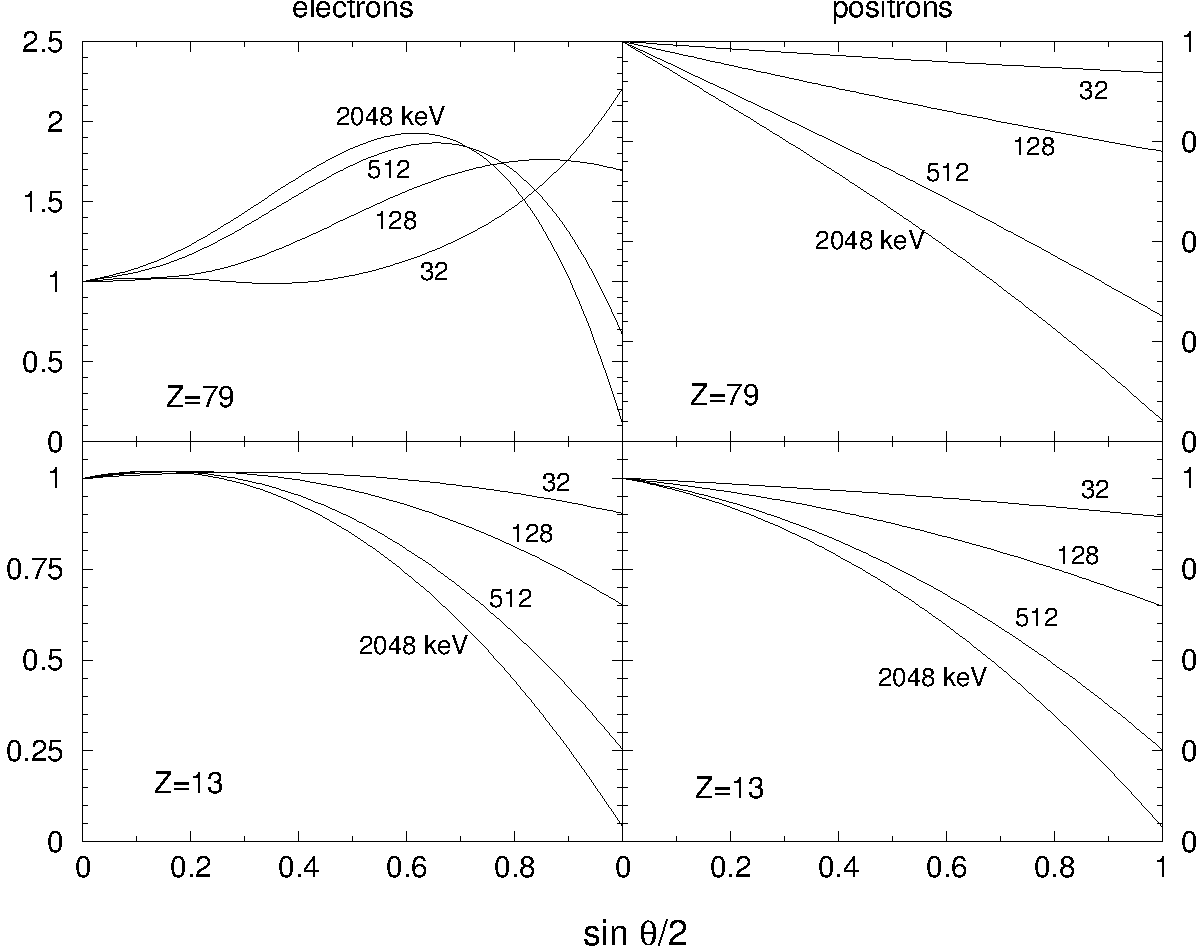
\includegraphics[height=14cm,width=14cm]{figures/mott1}
\index{Mott correction}
\caption[The Mott correction]{\label{fig_mott} The Mott correction factor
$R_{\rm mott}$ for gold and aluminum and various incident
electron and positron energies.}
\end{figure}

Berger and Wang \cite{BW89} have implemented into ETRAN (see {\em e.g.}
Ref. \cite{Se89})
the treatment of multiple
elastic scattering according to the general Mott PWA cross section,
equations \eqref{mott1} to \eqref{mott3}. They have used the code
by Riley \cite{Ri74} for the numerical solution of Eq. \eqref{mott2}
in a nuclear field screened by an electron density distribution
obtained from the multi-configuration Dirac-Fock program by
Desclaux \cite{De75}. These cross sections were later implemented
also in ITS \cite{ITSV3}. Note that ETRAN and ITS use a Class I
condensed history implementation where electron transport is
performed on  a pre-determined step-size grid. This allows
the calculation of the multiple elastic scattering distribution
(see section \ref{sec_MS}) for arbitrary complicated cross
sections for the step-size grid used with a reasonable amount
of pre-calculated data.

\index{Class II scheme!multiple scattering}
\index{Seltzer, Stephen}
The situation in a Class II code is more difficult as step-lengths
are stochastic (see section \ref{electron_general}).
Using Riley's code and Desclaux' electron
density functions, both kindly provided to us by Steve Seltzer of NIST,
we have also generated an elastic scattering data
base for all elements and energies from 1 keV to 16 MeV\footnote{
The calculation of the elastic scattering cross section from
equations \eqref{mott1} to \eqref{mott3} becomes increasingly
more difficult with increasing energy as more and more phase
shifts have to be calculated and numerical round-off errors
accumulate in the summations involved. We have modified Riley's
code to perform calculations in double precision, use more dense phase
shifts calculation grid and more accurate interpolations for
the electron density. This allowed calculations up to 16 MeV, for
even higher energies the results become numerically unstable.}.
Using this data base, we have studied the construction of a multiple
\index{multiple elastic scattering}
scattering theory but could not find a satisfactory procedure
to keep the amount of pre-calculated data required at a reasonable level.
We have therefore decided to approximate the elastic scattering
cross section as
\begin{equation}
\label{sigma_el}
{{\rm d}\sigma_{el} \over {\rm d}\mu} = {{\rm d}\sigma_{SR} \over {\rm d}\mu}
R_{\rm mott}(Z,\tau,\mu)
\end{equation}
\index{Mott correction}
where ${\rm d}\sigma_{SR}/{\rm d}\mu$ is the screened Rutherford cross
section given in Eq. \eqref{SR_1}. This approximation is known
to be accurate for energies above 1 MeV (high-$Z$ materials) or
100 keV (low-$Z$ materials) as there the spin effect correction
decouples from the screening correction \cite{BW89}. To
reproduce the average scattering at low energies we treat
the screening parameter $\eta$ as a free parameter and determine
it by numerically solving the equation
\begin{equation}
\label{fix_eta}
\int\limits_{-1}^1 {\rm d} \mu {{\rm d}\sigma_{SR} \over {\rm d}\mu}
R_{\rm mott}(Z,\tau,\mu) (1 - \mu) \equiv
\int\limits_{-1}^1 {\rm d} \mu {{\rm d}\sigma_{\rm PWA} \over {\rm d} \mu}
(1 - \mu)
\end{equation}
\index{screening parameter}
The resulting screening parameter for electrons is shown
as a function of $\beta$ for 4 different elements in
Fig. \ref{fig_eta}. In this figure $\eta$ is expressed in units
of $\eta_{\rm M}$, where
\begin{equation}
\label{eta_M}
\eta_{\rm M} = \eta_0 (1.13 + 3.76 \alpha^2 Z^2)
\end{equation}
is the screening parameter used in EGS4.
\begin{figure}[htp]
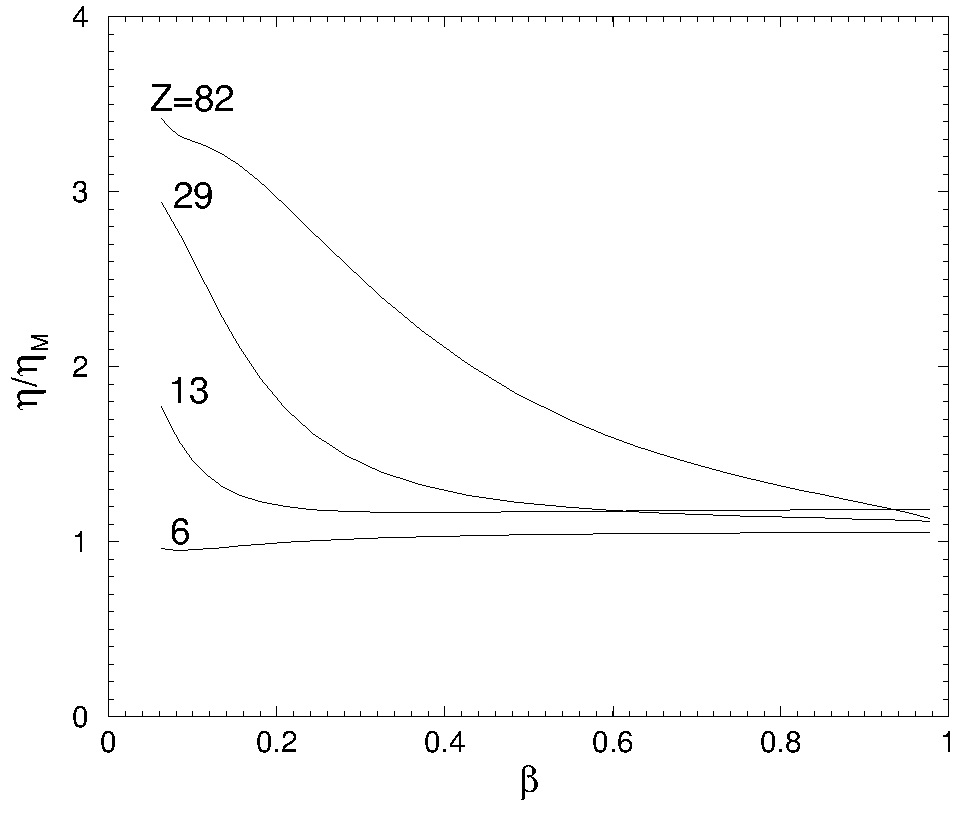
\includegraphics[height=12cm,width=12cm]{figures/eta}
\caption[Screening parameter]{\label{fig_eta} The screening parameter $\eta$,
determined from Eq. \protect\eqref{fix_eta}, in units of
$\eta_{\rm M}$, defined in Eq. \protect\eqref{eta_M}.}
\end{figure}

The elastic scattering cross section for compounds and
mixtures is expressed in a similar form as Eq. \eqref{sigma_el}
but now the Mott correction is
\begin{equation}
R_{\rm mott}(\tau,\mu) = {\sum p_i Z_i^2 R_{\rm mott}(Z_i,\tau,\mu) \over
\sum p_i Z_i^2}
\end{equation}
and the screening parameter is determined from Eq. \eqref{fix_eta} where
the partial-wave analysis cross section for the compound is
calculated from the PWA cross sections of its elements using
the independent atom approximation.

\index{angular deflections!inelastic collisions}
We can now turn to the discussion of the modifications necessary
to take into account contributions from angular deflections
due to sub-threshold processes. Various studies on this subject
are available in the literature, see {\em e.g.} \cite{Sc63,Fa54,BW89}.
We have not attempted to implement one of them, instead, we
take the simplistic point of view that the contributions
to angular deflections for all inelastic collisions, sub-threshold
and discrete, can be taken into account by replacing
$Z^2$ with $Z (Z + \xi_{0})$ in the screened Rutherford
cross section, Eq. \eqref{SR_1}. Here $\xi_0$ is an appropriate
parameter, we use by default $\xi_0=1$ but this is not a necessary
requirement. If now inelastic collisions with energy transfer
larger than $T_c$ are simulated explicitly, $\xi_0$ must
be replaced with an energy and cut-off dependent parameter $\xi(T,T_c)$
as follows \cite{Ka96c}
\begin{equation}
\xi(T,T_c) = \xi_0 \left(1 - {1 \over \bar{Z} + \xi_0}~
{g_{\rm M}(\tau,\tau_c) \over g_{\rm R}(\eta) } \right)
\end{equation}
where $\bar{Z}$ is the average atomic number of the compound
and %$g_{\rm M}(\tau,\tau_c)$ is the average angle
\newcommand{\tpr}{\tau^{\prime}}
\begin{equation}
\begin{split}
g_M(\tau,\tau_c) & =
\ln {\tau \over 2 \tau_c} + \left[1 +
{(\tau + 2)^2 \over (\tau+1)^2} \right] \ln {2 (\tau-\tau_c+2) \over \tau + 4}
\\ &-
\left[{(\tau+2)^2 \over 4} + {(\tau+2) (\tau+1/2) \over (\tau+1)^2} \right]
\ln {(\tau+4) (\tau-\tau_c) \over \tau (\tau-\tau_c+2)} \\ & +
{(\tau-2 \tau_c) (\tau+2) \over 2}
\left[{1 \over \tau-\tau_c} - {1 \over (\tau+1)^2} \right]~.
\end{split}
\end{equation}
($\tau_c = T_c/m$) and
\begin{equation}
g_{\rm R}(\eta) = (1 + 2 \eta) \left[ \ln \left(1 + \frac{1}{\eta} \right) - 2
\right]
\end{equation}

\index{SPIN\_EFFECTS}
To summarize, when spin effects are turned on in EGSnrc
({\tt SPIN\_EFFECTS = .true.}), the elastic scattering
cross section used is
\begin{equation}
\label{sigma_el1}
{{\rm d}\sigma_{\rm el} \over {\rm d}\mu} =
{2 \pi r_0^2 Z (Z + \xi(T,T_c)) \over
\beta^2 \tau (\tau + 2) }~{R_{\rm mott}(Z,T,\mu) \over (1 - \mu + 2 \eta)^2}
\end{equation}
where
\begin{itemize}
\item
The screening parameter $\eta$ is determined from the requirement
that the above cross section reproduces the average scattering
from PWA cross sections obtained via the numerical solution of
equations \eqref{mott1} to \eqref{mott3} using Hartree-Fock
electron densities. This parameter is different for electrons
and positrons
\item
The parameter $\xi(T,T_c)$ takes into account contributions
from sub-threshold inelastic collisions, it depends on energy
and the threshold energy $T_c$
\item
$R_{\rm mott}$ is the Mott correction that is the result of
the solution of the Dirac equation in the field of a bare nucleus.
\end{itemize}
All parameters necessary for the run-time interpolation
of $\eta$, $\xi$ and $R_{\rm mott}$ are initialized in
the subroutine {\tt init\_spin} which is called from
the subroutine {\tt mscati}, executed at the end of {\tt HATCH}.

Sampling of single elastic scattering events on the basis of
Eq. \eqref{sigma_el1} is performed using a rejection technique.
One uses Eq. \eqref{sample_SR} to sample the screened Rutherford
part, the $\mu$ sampled is accepted if a second random number is
less than $R_{\rm mott}/R_{\rm mott,max}$. The efficiency of
this algorithm is close to unity for low-$Z$ materials but
only close to $1/2$ for high-$Z$ materials.

\subsubsection{Multiple elastic scattering}
\label{sec_MS}
\setcounter{equation}{0}
\index{multiple elastic scattering}
\index{Goudsmit-Saunderson theory}

The multiple elastic scattering distribution for electron
transport in an infinite, homogeneous medium for a path-length
$s$, which corresponds to an energy loss $E_0 - E$, can be obtained
from Eq. \eqref{transport3} by integrating it over the position,
expanding $\Phi_0$ and the cross sections in Legendre polynomials
$P_l$ to arrive at
\begin{equation}
\Phi_0(\mu,\phi,E) = \frac{1}{2 \pi} \sum_{l=0}^\infty \left(l + \frac{1}{2}
\right) \exp( -G_l ) P_l(\mu)
\end{equation}
where $\mu$ is the cosine of the polar angle $\theta$ and the process
is considered in a frame where the electron is initially moving
along the $z$ axis. This expression was first obtained by
Goudsmit and Saunderson \cite{GS40,GS40a}. The Goudsmit-Saunderson
(GS) moments $G_l$ are given by
\begin{equation}
\label{GS_moments}
G_l = \int\limits_0^s {\rm d}s' \kappa_l(s') =  \int\limits_{E}^{E_0}
{{\rm d}E' \over L(E',E_c,k_c)} \kappa_l(E')
\end{equation}
where the $\kappa_l$ denote the moments of the elastic scattering
cross section,
\index{elastic scattering!moments}
\begin{equation}
\label{kappa_l}
\kappa_l(E) = 2 \pi
\int\limits_{-1}^1 {\rm d}\mu
\Sigma_{\rm el}'(\mu,E) \left[ 1 - P_l(\mu) \right] ~.
\end{equation}
The moments $\kappa_l$ depend on the energy and the material in
which the transport takes place, so that the
multiple elastic distribution is dependent on the energy,
path-length (or corresponding energy loss), material, and
threshold energies for discrete interactions. In a Class I
condensed history implementation one uses the total stopping
power (because discrete interaction are not explicitely modelled).
In addition, possible path-lengths are limited to the
energy-loss grid which is decided upon prior to the simulation.
These two facts allow the MS distributions to be pre-computed
and stored in the memory using a relatively small amount of
data. In a Class II implementation path-lengths are stochastic
and so a straightforward pre-calculation for all possible step-lengths
is not possible. In the past this fact has favoured use of
\index{multiple elastic scattering!small-angle approximation}
small-angle theories for the modelling of multiple elastic
scattering, {\em e.g.} the theory of \Mol~ which is used in EGS4.
The limitations of \Mol's theory have been discussed extensively
in the literature.

In EGSnrc we use an exact formulation, the multiple scattering
distributions employed being dependent on the underlying
elastic scattering cross sections (see section \ref{elastic}).

\paragraph{Multiple elastic scattering from the screened Rutherford
cross section} \hfill

\index{screened Rutherford cross section}
\index{multiple elastic scattering!based on screened Rutherford}
The multiple elastic scattering theory for the screened
Rutherford cross section employed in EGSnrc was developed
by Kawrakow and Bielajew in Ref. \cite{KB97} and later refined
by Kawrakow in Ref. \cite{Ka99a} to better take into account
energy loss.

The treatment of Ref. \cite{KB97} starts with the MS distribution
that results from the neglect of energy loss which can be written
as
\begin{equation}
2 \pi \Phi_0(\mu,\phi,E) = e^{-\lambda} \delta(1 - \mu)
+ \lambda e^{-\lambda} {1 \over \sigma_{\rm SR}}
{{\rm d} \sigma_{\rm SR}(\mu) \over {\rm d}\mu} +
\left(1 - e^{-\lambda} - \lambda e^{-\lambda} \right) F^{(2+)}_{\rm SR} (\mu)
\end{equation}
where $\lambda$ is the number of elastic free paths corresponding
to the path-length $s$,
\begin{equation}
\label{lambda}
\lambda = \Sigma_{SR} s~,
\end{equation}
and the screened Rutherford cross section
is given in Eq. \eqref{SR_1}.
The distribution $F^{(2+)}_{\rm SR}$ is the normalized multiple
scattering distribution
that results from at least two elastic collisions described by
the screened Rutherford cross section,
\index{screened Rutherford cross section}
\begin{equation}
\label{F_2plus}
\begin{split}
F^{(2+)}_{\rm SR}(\mu) & = \sum_{l=0}^\infty \left(l + \frac{1}{2} \right)
P_l(\mu) j_l^{(2+)}  \\
j_l^{(2+)} & = { \exp(-G_{l, {\rm SR}}) +
\left[ 1 + \lambda - G_{l,{\rm SR}} \right] \exp(-\lambda)
\over 1 - \exp(-\lambda) - \lambda \exp(-\lambda) }
\end{split}
\end{equation}
Here, we have put the subscript ``SR'' on the moments $G_l$
to explicitly state that they are calculated
using the screened Rutherford cross section.
Equation \eqref{F_2plus} can be put in a more tractable form
by a variable change,
\index{screened Rutherford cross section}
\begin{equation}
u = (1 + a) \left(1 - {2 a \over 1 - \mu + 2 a} \right)
\end{equation}
where the parameter $a$ is chosen such as to make $q^{(2+)}_{\rm SR}$,
\begin{equation}
q^{(2+)}_{\rm SR}(u) = F^{(2+)}_{\rm SR}(\mu)~{{\rm d} \mu \over {\rm d} u}~,
\end{equation}
``as flat as possible''. After some
straightforward manipulations one obtains \cite{KB97}
\begin{equation}
\label{a-kappa}
a = \kappa + \sqrt{\kappa^2 + \kappa}
\end{equation}
with the short hand notation
\begin{equation}
\label{kappa}
\begin{split}
\kappa & = {\langle 0\rangle - 2 \langle 1\rangle +
          \langle 2\rangle \over 4 \langle 1\rangle } \\
\langle n\rangle & =
\sum_{l=0}^\infty \left( l + {1 \over 2} \right) j_l^{(2+)}
      \sum_{m=0}^\infty \left( m + {1 \over 2} \right) j_m^{(2+)}
      \int_{-1}^1 {\rm d} \mu~ \mu^n P_l(\mu) P_m(\mu)~,
\end{split}
\end{equation}
The quantity $\omega^2 = a/\eta$ ($\eta$ is the screening parameter)
is a function of $\lambda$ and has a slight dependence
on $\eta$. In terms of simulation efficiency, it is better to
ignore the $\eta$ dependence of $\omega$ and use a fit to
the data obtained  at run time from Eq. (\ref{a-kappa},\ref{kappa}) for
$\eta \to 0$. We use
\begin{equation}
\label{fit_omega2}
\begin{split}
{\omega^2 \over \lambda + 4} & =
\begin{cases}
1.347 + t (0.209364 - t (0.45525 - t (0.50142 - 0.081234 t))) & \text{if}~
\lambda < 10, \\
-2.77164 + t (2.94874 - t (0.1535754 - 0.00552888 t)) & \text{else}
\end{cases}
\\
t & = \ln \lambda
\end{split}
\end{equation}
The dependence of the distribution $q^{(2+)}_{\rm SR}(u)$ on
$\lambda$ and $\eta$
\begin{figure}[htp]
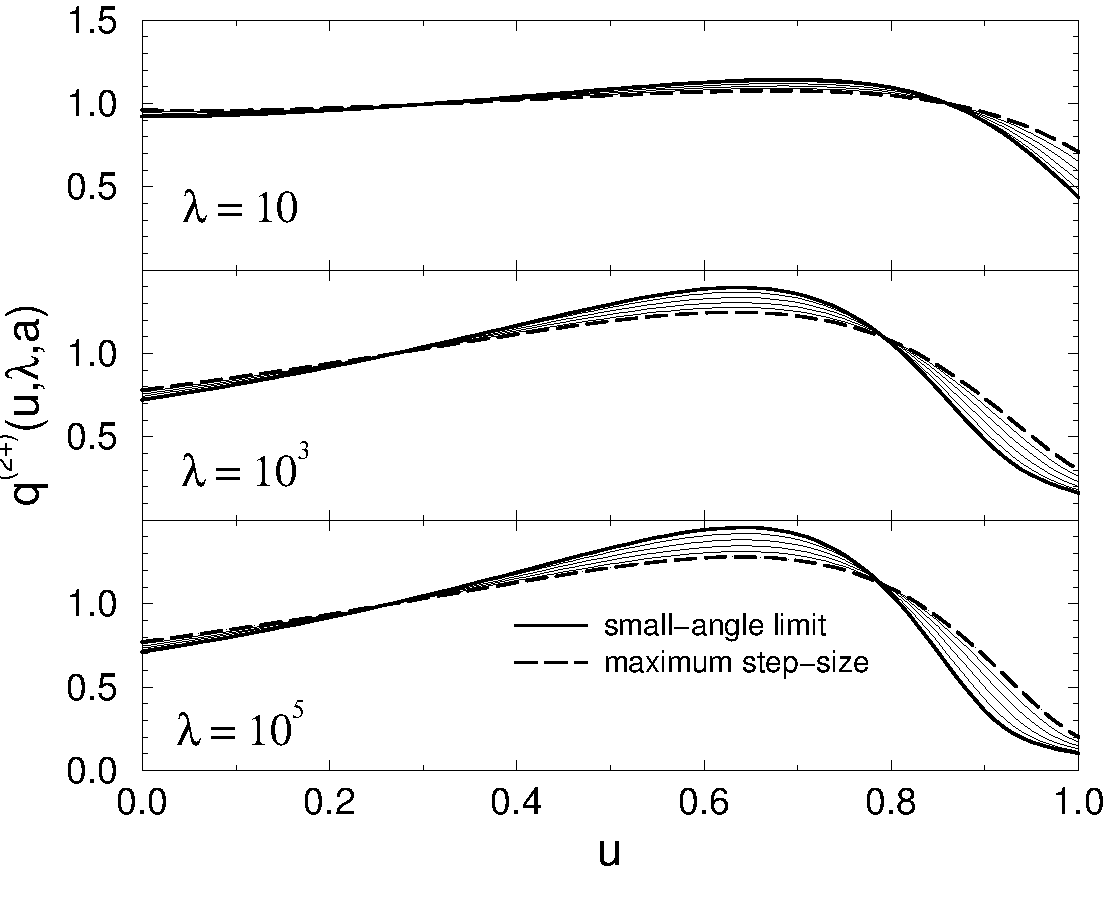
\includegraphics[height=15cm,width=15cm]{figures/q2}
\caption[The $q^{(2+)}$ surface]{\label{fig_q2}
The $q^{(2+)}_{\rm SR}$ distribution for
three step-lengths. The curve labelled ``small-angle'' limit is
the distribution for $\eta \to 0$ (infinite energy), the
curve for the maximum step-size corresponds to the
maximum step-size for condensed history steps for which the data base was
generated ($G_1 < 0.5$, see section~\ref{es_algorithm}.)}
\end{figure}
is rather weak, as can be seen in Fig. \ref{fig_q2}.
$q^{(2+)}_{\rm SR}$ can therefore be interpolated
very accurately during run time using
linear interpolation in $\ln \lambda$ and $G_{1,{\rm SR}}$
from a pre-computed table.
Here $G_{1,{\rm SR}}$ denotes the first
GS moment, see Eq. \eqref{GS_moments}, resulting
from screened Rutherford elastic scattering,
\index{screened Rutherford cross section}
\begin{equation}
\label{G1_SR}
G_{1,{\rm SR}} =
2 \lambda \eta \left[ (1 + \eta) \ln\left(1 + \frac{1}{\eta}\right) - 1
\right]
\end{equation}
The $q^{(2+)}_{\rm SR}$ data which are in a form of a 3 dimensional
alias table, are stored in the file {\tt newms.data} and read in
by subroutine {\tt init\_ms\_SR}.

\index{multiple elastic scattering!energy loss}
To take into account energy loss, one uses the multiple scattering
distribution for an ``effective'' step energy which is
determined from the requirement \cite{Ka99a}
\begin{equation}
{G_2(E_0,E) \over G_1(E_0,E)} =
{\kappa_2(E_{\rm eff}) \over \kappa_1(E_{\rm eff})}
\end{equation}
for a path-length $s_{\rm eff}$,
\begin{equation}
s_{\rm eff} = {G_1(E_0,E) \over \kappa_1(E_{\rm eff})}~.
\end{equation}
These two requirements guarantee that the first two GS moments
are exactly reproduced, and gives at the same time a very accurate
approximation for higher order GS so that the resulting
multiple scattering distribution is virtually
identical to the MS distribution calculated via numerical integration
of the moments $G_l$, see Fig. 2 of Ref. \cite{Ka99a}.

\index{screened Rutherford cross section}
For the screened Rutherford cross section the effective energy and
path-length are given by
\begin{eqnarray}
\label{E-eff}
E_{\rm eff} & = & E_0 \left[ 1 - {\epsilon \over 2} -
{\epsilon^2 \over 12 (2 - \epsilon)} \left(
{5 \tilde{\tau}^2 + 10 \tilde{\tau} + 6 \over (\tilde{\tau} + 1)
(\tilde{\tau} + 2)} + 2 b(\tilde{E}) \right) + O(\epsilon^3) \right]
\nonumber \\
s_{\rm eff} & = & s \left( 1 - {\epsilon^2 \over 3 ( 2 - \epsilon)}~
{\tilde{\tau}^4 + 4 \tilde{\tau}^3 + 7 \tilde{\tau}^2 + 6 \tilde{\tau}
+ 4 \over (\tilde{\tau} + 1)^2 (\tilde{\tau} + 2)^2} + O(\epsilon^4) \right)
\end{eqnarray}
where we have defined
\begin{equation}
\label{bE}
b(E) = {E \over C(E)}~
{{\rm d} C(E) \over {\rm d}E~}~,\quad \quad C(E) = L(E) \beta^2~,
\end{equation}
$\beta$ denoting the particle velocity in units of the speed of light.
In the above equations $\epsilon = (E_0 - E)/E$ and $\tilde{\tau} =
1/2 (E_0 + E)/m$.

\index{multiple elastic scattering!sampling of}
With all this, the algorithm for sampling multiple elastic scattering
angles is as follows:
\begin{enumerate}
\item
Calculate $s_{\rm eff}$ and $E_{\rm eff}$ from Eq. \eqref{E-eff}.
\item
Calculate $\lambda$ from Eq. \eqref{lambda} and \eqref{SR_tot},
$t = \ln \lambda$  and $\eta$ from Eq. \eqref{calc_eta}
\item
Pick a random number number $r_1$.
\item
If $r_1 < e^{-\lambda}$, then the scattering angle is zero, return
control to the calling routine
\item
Else if $r_1 < e^{-\lambda}(1 + \lambda)$, then sample $\mu$ from
the single scattering distribution according to Eq. \eqref{sample_SR},
return
control to the calling routine
\item
Else, we must sample $\mu$ from the $q^{(2+)}_{\rm SR}$ distribution.
Calculate $G_{1,{\rm SR}}$ from Eq. \eqref{G1_SR},
$\omega^2$ from Eq. \eqref{fit_omega2} and
$a = \omega^2 \eta$
\item
Determine the table look-up indices for $\ln \lambda$ and $G_{1,{\rm SR}}$
\item
Sample $u$ from the corresponding $q^{(2+)}_{\rm SR}(u)$ distribution
\item
Deliver $\mu$,
\begin{equation}
\mu = {2 a u \over 1 - u + a}
\end{equation}
\end{enumerate}


\paragraph{Multiple elastic scattering with spin effects} \hfill

\index{multiple elastic scattering!spin effects}
\index{screened Rutherford cross section}
In principle, the approach developed in Ref. \cite{KB97} could
be applied to more complicated single elastic scattering cross
sections than the screened Rutherford cross section.
We have found, however, that the direct use of this approach for
the cross section with spin effects (see section \ref{spin_elastic})
does not lead to a satisfactory interpolation accuracy. We have
therefore implemented a rejection technique for the sampling
of multiple scattering angles when {\tt SPIN\_EFFECTS = .true.}.
\index{SPIN\_EFFECTS}

We can write the multiple scattering distribution
that results from at least 2 elastic scattering processes as
\index{screened Rutherford cross section}
\begin{equation}
\label{ms_spin1}
F^{(2+)}(\lambda,\eta,Z,\mu) = F^{(2+)}_{\rm SR}(\lambda,\eta,\mu)
R(\lambda,\eta,Z,\mu)
\end{equation}
where $F^{(2+)}_{\rm SR}$ is the 2+ distribution from a
screened Rutherford cross section for a path-length corresponding
to $\lambda$ elastic mean-free paths and a screening angle $\eta$
and $R(\lambda,\eta,Z,\mu)$ is defined as
\begin{equation}
 R(\lambda,\eta,Z,\mu) = {F^{(2+)}(\lambda,\eta,Z,\mu) \over
F^{(2+)}_{\rm SR}(\lambda,\eta,\mu)}
\end{equation}
({\em i.e.} Eq. \eqref{ms_spin1} is the identity $F^{(2+)}=F^{(2+)}$).
The function $R(\lambda,\eta,Z,\mu)$ is a three dimensional
surface for each medium.
Numerical experiments show that the way which requires the minimum
amount of pre-calculated data to interpolate
the function $R(\lambda,\eta,Z,\mu)$ between pre-calculated
data is to use for each medium
\begin{itemize}
\item
Linear interpolation in the quantity $q$,
\begin{equation}
q = {2 G_{1,{\rm SR}}(\lambda,\eta) \over 1 + 2 G_{1,{\rm SR}}(\lambda,\eta)}~.
\end{equation}
Obviously $q$ can take only values between zero and unity. For
$q \to 0, R(\lambda,\eta,Z,\mu)$ converges to $R_{\rm mott}(E,Z,\mu)$,
see section \ref{spin_elastic}. For $q \to 1, R(\lambda,\eta,Z,\mu)$
goes to unity for all angles $\mu$. The rate at which the function
$R$ changes from the one limit to the other depends on the energy.
\item
Linear interpolation in $\beta^2$ for energies greater than
100 keV, linear interpolation in $\ln E$ for energies less
then 100 keV.
\item
Linear interpolation in $\sin \theta/2 = \sqrt{(1-\mu)/2}$.
\end{itemize}
The pre-calculated data are stored in separate files for
all elements in the directory {\tt spinms} and used
in subroutine {\tt init\_spin} to compute $R$ for
the media involved in the actual simulation. {\tt init\_spin}
is called from {\tt mscati} which is called from {\tt HATCH}.

The sampling algorithm is then similar to the one given at the
and of the previous section but involves an additional rejection
loop in steps 4 and 8 using $R_{\rm mott}$ or $R$ as a
rejection function\footnote{Both, $R_{\rm mott}$ and $R$ are
scaled to their maximum in the routine {\tt init\_spin}.}.
In addition, the calculation of the screening parameter
$\eta$ and the number of mean-free-paths $\lambda$ involve
additional correction factors, because both, $\eta/\eta_0$ and
the parameter $\xi$ which describe the contribution
of sub-threshold inelastic collisions to angular deflections,
are not constant, see section \ref{spin_elastic}.

\index{spin effects!measurements}
It is worth showing an example of the influence of the inclusion
of spin effects in the treatment of elastic scattering as
a conclusion of this section.
\begin{figure}[htp]
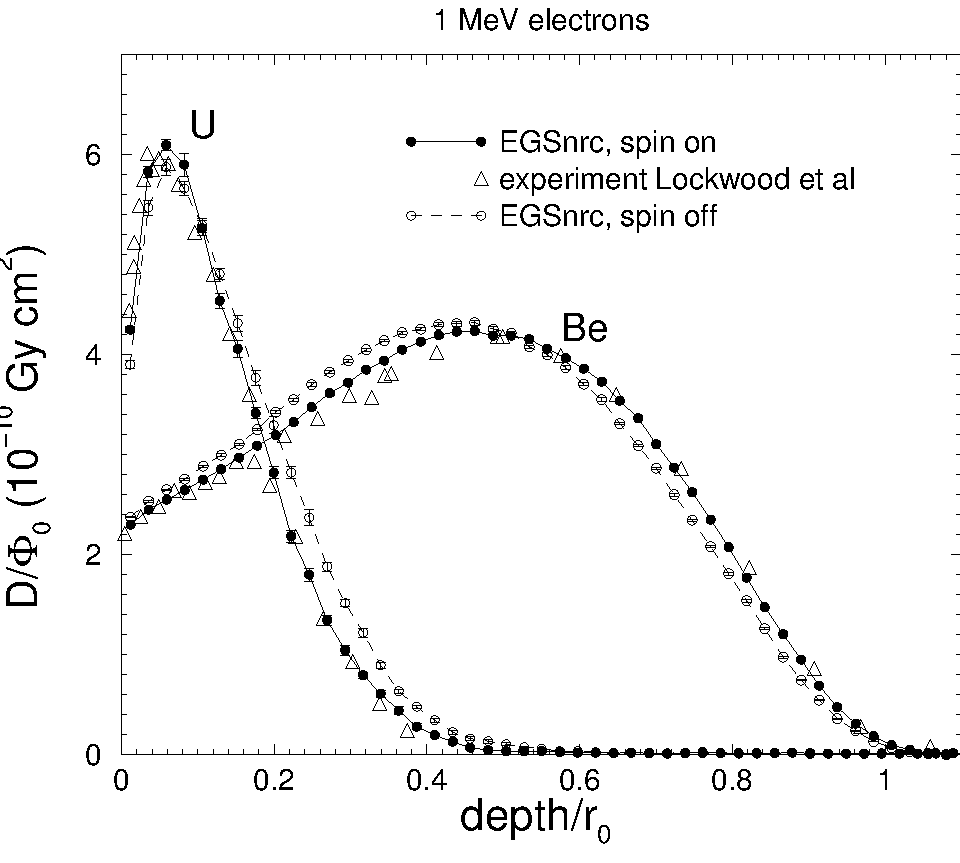
\includegraphics[height=12cm,width=12cm]{figures/dd_1MeV_Be_and_U}
\caption[Depth-dose curves in Beryllium and Uranium]{\label{dd_spin}
Depth-dose curves
for a broad parallel beam of 1 MeV electrons incident
on a Beryllium or Uranium target as a function of the CSDA range.
The experimental data are from \protect\cite{Lo80a}.}
\end{figure}
Figure \ref{dd_spin} shows a comparison of calculated depth-dose curves
in Beryllium and Uranium to measurements by Lockwood {\em et al} \cite{Lo80a}.
Both, the calculations and the measurements are absolute.
The calculations with ``spin on'' are in much better agreement
with the experiment. The effect of including spin is
to make the effective range of electrons longer for low-$Z$
materials and shorter for high-$Z$ materials. It is also
present for the energy range relevant for radiation therapy.
The reason for not seeing disagreement between EGS4 calculations
and measurements in this energy range is due to the rarity of
measurements
with precise knowledge of the incident energy. In depth-dose measurements
with a known 20 MeV electron beam incident on water, comparisons to EGS4
required using an incident beam energy of 20.3 MeV to get good
agreement\cite{Ro95}. In contrast, the calculations with EGSnrc with spin
turned on are in good
agreement with the measurements when using an incident energy of 20.0 MeV,
in agreement with the known energy.

\subsubsection{Electron-step algorithm}
\label{es_algorithm}
\setcounter{equation}{0}
\index{electron-step algorithm}

As mentioned in section \ref{electron_general},
the transport between
subsequent ``catastrophic'' collisions is described by
Eq. \eqref{transport3} with Eq. \eqref{s_vs_E} providing
the link between energy and path-length. An exact solution
of this equation is not known and so some approximate
methods are required to relate the
energy loss, the path-length, and the spatial displacement.

The simplest possible
approach one could take is to ignore deflections due
to multiple elastic scattering
during the condensed history step and
to transport the electron on a straight line along the initial
direction of motion. In order for this approach to
be accurate the CH steps must be sufficiently short so
that the straight line approach does not represent to a
severe approximation. Larsen has shown \cite{La92} that
any condensed history algorithm will converge to the correct
answer in the limit of sufficiently small step-sizes, provided
multiple elastic scattering is faithfully simulated.
However, making the step lengths very short may
cause the simulation to become extremely inefficient.
In addition, if the calculated results show step-size
dependencies, one needs to perform a careful step-size
study in order to determine when the result has
converged.

Many electron-step algorithms that attempt to make
corrections for deflections from the straight-line
approach have been proposed over the years, {\em e.g.}
\cite{Be63,BR87,Fe93,Ka96b}. A detailed discussion of these
algorithms is given in Ref. \cite{KB97a}.  In general
none of the algorithms available is accurate enough
to allow the condensed history simulation between
subsequent discrete events to be always done in a single
step. Instead, the distances between discrete collisions
is divided into smaller condensed history steps using
a procedure to determine maximum acceptable
lengths for the steps (step-size restrictions).
\index{step-size restrictions}

\index{trans\-port\_algo\-rithm}
%\index{{\tt trans\-port\_algo\-rithm}}
\index{path-length correction}
\index{lateral correlation algorithm}
\index{PRESTA}
The electron-step algorithm employed in EGSnrc depends
on the parameter {\tt trans\-port\_algo\-rithm} which
is in {\tt COMMON/ET\_Control/}. If set
to one, a slightly modified version of
PRESTA's \cite{BR87} path-length-correction (PLC)
and lateral correlation algorithm (LCA) are employed.
The PRESTA algorithm is known to underestimate
lateral deflections (deflections perpendicular to the
initial direction of motion), to underestimate
longitudinal straggling and to produce a singularity
in the distribution describing the lateral spread of electrons
in a single condensed history step \cite{Ka96b,KB97a}.
The implications on the simulation results depend on
the actual situation under investigation. At high energies,
where elastic scattering is weak, PRESTA is perhaps sufficiently
accurate. Its use for low energy applications is not
recommended. One of us has shown, for instance, that
there is up to 8\% variation of the calculated ion chamber
response subject to a $^{60}Co$ beam when using PRESTA's
transport algorithm \cite{Ka99b}.

If the parameter {\tt trans\-port\_algo\-rithm} is set to zero
(it's default value), the electron-step algorithm
developed in Ref. \cite{KB97a} and later refined in
\cite{Ka99a} is employed. This algorithm is constructed
in such a way as to reproduce up to second order spatial moments
of the fluence $\Phi_0(\vec{x},\vec{\Omega},E,t)$, which
are known from the theory of Lewis \cite{Le50} for
transport in an infinite, homogeneous medium. This algorithm
was shown to produce step-size independent results for
ion chamber simulations and backscattering \cite{Ka99a,Ka99b}, two of the
most difficult tasks for condensed history Monte Carlo codes.

For completeness, we give a brief summary of the transport
algorithms available in EGSnrc. Final positions are in a frame
where the electron is initially at the origin and moving
along the positive z-axis. Positions in the actual simulation
co-ordinate system are obtained using the appropriate
rotations and spatial translations.
\begin{itemize}
\index{PRESTA}
\item
{\tt trans\-port\_algo\-rithm = 1} (PRESTA)
\begin{equation}
\label{PRESTA}
\begin{split}
x &= r_\perp \sin \theta \cos \phi \\
y &= r_\perp \sin \theta \sin \phi \\
z &= \langle z \rangle \\
r_\perp &= \mbox{Min}\left({s \over 2},\sqrt{{s^2 - \langle z \rangle^2 \over
\sin^2 \theta}} \right)
\end{split}
\end{equation}
where $\theta$ and $\phi$ are the polar and azimuthal scattering
angles and $\langle z \rangle$ the average transport distance
in the initial direction of motion for a path-length of $s$.
In the original PRESTA implementation $\langle z \rangle$
was calculated from the theory of \Mol, we use in EGSnrc the
exact expression of Lewis \cite{Le50}, which is simply
\begin{equation}
\langle z \rangle = s~{1 - \exp(-G_1) \over G_1}
\end{equation}
if one neglects energy loss. A small correction arises
if energy loss is taken into account, it is not included
to be consistent with PRESTA where energy loss was also ignored.
\item {\tt trans\-port\_algo\-rithm = 0} (EGSnrc default) \hfill \\
The condensed history step is divided into two sub-steps and
separate multiple elastic scattering angles $\theta_1,\phi_1$ and
$\theta_2,\phi_2$ are sampled. The final scattering angle
is then determined from $\theta_1,\phi_1$,$\theta_2,\phi_2$, {\em e.g.}
\begin{equation}
\cos \theta = \cos \theta_1 \cos \theta_2 - \sin \theta_1 \sin \theta_2
\cos(\phi_1 - \phi_2)~.
\end{equation}
The final position is calculated as follows:
\begin{equation}
\label{egsnrc_algorithm}
\begin{split}
x & = s \Big[ \eta \delta \sin \theta_1 \cos \phi_1 +
\eta (1 - \delta) \sin \theta_2 ( \cos \phi_1 \cos \phi_2 -
\cos \theta_1 \sin \phi_1 \sin \phi_2 ) +
a_2 \sin \theta \cos \phi \Big] \\
y & = s \Big[ \eta \delta \sin \theta_1 \sin \phi_1 +
\eta (1 - \delta) \sin \theta_2 ( \sin \phi_1 \cos \phi_2 +
\cos \theta_1 \cos \phi_1 \sin \phi_2 ) +
a_2 \sin \theta \sin \phi \Big] \\
z & = s \Big[ a_1 + \eta \delta \cos \theta_1 +
\eta (1 - \delta) \cos \theta_2 +
a_2 \cos \theta \Big] \\
a_1 & = {1 - \eta \over 2} (1 + \alpha_1) \\
a_2 & = {1 - \eta \over 2} (1 - \alpha_1) \\
\delta & = {1 \over 2} + {\sqrt{6} \over 6} -
\left( {1 \over 4 \sqrt{6}} - \gamma {4 - \sqrt{6} \over 24 \sqrt{6}}
\right) G_1 + \alpha_2 \\
\gamma & = {G_2 \over G_1}
\end{split}
\end{equation}
Here, $\eta$ is a random number sampled from $2 \eta {\rm d} \eta$
(and not the screening parameter) and $\alpha_1$ and $\alpha_2$
are energy loss corrections derived in Ref. \cite{Ka99a},
\begin{equation}
\label{eloss_correction}
\begin{split}
\alpha_1 & = - {\kappa_1'(\tilde{E}) \over \kappa_1(\tilde{E})}~
{\Delta E \over 2} + O(\Delta E^2) \\
\alpha_2 & = \left( {\kappa_2'(\tilde{E}) \over \kappa_2(\tilde{E})}
- {\kappa_1'(\tilde{E}) \over \kappa_1(\tilde{E})} \right) {\Delta E \over
2 \sqrt{6} } + O(\Delta E^2)
\end{split}
\end{equation}
where $\Delta E$ is the sub-threshold energy loss associated
with the step, $\tilde{E}$ the average step energy and
$\kappa_1'$ and $\kappa_2'$ derivatives of the
moments $\kappa_1$ and $\kappa_2$ (see Eq. \eqref{kappa_l})
with respect to $E$.
\index{ximax}
\index{ESTEPE}
\index{$G_1$}
If elastic scattering is described by the screened Rutherford
cross section, the energy loss corrections $\alpha_1$ and
$\alpha_2$ are given by
\begin{equation}
\label{eloss_correction_SR}
\begin{split}
\alpha_1 & \approx \left( {2 + 2 \tilde{\tau} + \tilde{\tau}^2 \over
(1 + \tilde{\tau}) } - {1 + \tilde{\tau} \over
\ln(1 + 1/\tilde{\eta}) (1 + \tilde{\eta}) - 1) } \right)
{\Delta E/\tilde{E} \over  (2 + \tilde{\tau})}
\\
\alpha_2 & \approx {\Delta E/\tilde{E} \over \sqrt{6} (1 + \tilde{\tau})
(2 + \tilde{\tau}) \Big[
\ln(1 + 1/\tilde{\eta}) (1 + \tilde{\eta}) - 1) \Big]
\Big[ \ln(1 + 1/\tilde{\eta}) (1 + 2 \tilde{\eta}) - 2) \Big] }
\end{split}
\end{equation}
where $\tilde{\tau} = \tilde{E}/m$ and
$\tilde{\eta}$ is the screening parameter for
the midpoint energy $\tilde{E}$.
These equations are used in the subroutine {\tt msdist\_pII}
which implements condensed history electron transport according
to the algorithm given in Eq. \eqref{egsnrc_algorithm}.
Strictly speaking, when spin effects are ``turned on'', one
should use the energy loss corrections derived
from the moments resulting from the corresponding elastic scattering
cross section. We have left this refinment for the future because
(i) Given the fact that the corrections involve the calculation
of derivatives and that the cross sections with spin are
available only in numerical form, the implementation is more
difficult (ii) Eq. \eqref{eloss_correction_SR} does take into
account the main energy dependence of the corrections, deviations
from Eq. \eqref{eloss_correction_SR} are either higher order
in $\Delta E$ or have small coefficients.

The algorithm given in Eq. \eqref{egsnrc_algorithm} reproduces
first and second order spatial moments to better than 0.1\% for
$G_1 \le 0.5$ if energy loss is neglected ($G_1$ is defined by Eq.
\eqref{GS_moments} and is a function of pathlength, so this condition
imposes a maximum allowed step size). This accuracy
is maintained when energy loss is taken into account via
the corrections given in \eqref{eloss_correction} if
the maximum fractional energy loss per step is
restricted to 25\%. These two condensed history
step-size restrictions are controlled via the
parameters {\tt ximax} (corresponding to the maximum allowed $G_1$)
and {\tt ESTEPE} which are in {\tt COMMON/ET\_Control} and set by default
to 0.5 and 0.25.

Due to the use of the energy loss corrections derived from the
screened Rutherford cross section also for elastic scattering
with spin, in this case the deviation from the theoretical expectation
is slightly larger and exceeds 0.1\% for {\tt ESTEPE} between
0.15 and 0.2. If such a high precision is required for
your application, the simplest solution is to use step sizes
that don't exceed 20\% energy loss per step when spin is on.
\end{itemize}

%If one expands
%Eq. \eqref{transport3} in spherical harmonics,
%\begin{equation}
%\Phi_0(\vec{x},\vec{\Omega},s) = \sum\limits_{l m}
%f_{l m}(\vec{x},s) Y_{l m}(\vec{\Omega})~,
%\end{equation}
%the elastic scattering cross section in Legendre polynomials,
%and uses the addition theorem and the orthogonality, orthogona

\subsubsection{Boundary crossing algorithm}
\label{BCA}
\setcounter{equation}{0}
\index{boundary crossing algorithm}

The electron-step algorithms discussed in section
\ref{es_algorithm} are valid only for transport in
an infinite, homogeneous medium. In practical
situations one has to deal with interfaces between
different materials. If an electron is close
to an interface with another material, portions
of its curved path may be in this different material and
so the trajectory different than simulated.
In the original EGS4 version, this problem associated
with the condensed history simulation of electron
transport, which has become known as the interface artifact \cite{Bi85}, was
entirely ignored.
To address the interface artifact,
a refined boundary crossing algorithm (BCA) was
incorporated into PRESTA. According to this algorithm, the electron
is not allowed to take a step longer than $t_\perp$, $t_\perp$ being
the perpendicular distance to the closest boundary, unless
$t_\perp$ becomes smaller than $t_{min}$, a user defined
minimum step-length for boundary crossing. For $t_\perp < t_{min}$,
lateral deflections are switched off and the particle is transported,
as in the case of standard EGS4, on a straight line to the
boundary.
\index{PRESTA}

\index{boundary crossing algorithm!fluence singularity}
In a more recent paper \cite{FS95}, Foote and Smyth have demonstrated
that the approach of forcing a multiple scattering event at the
boundary causes a singularity in the simulated particle fluence.
The singularity results from the fact that there is a
non-zero probability for scattering parallel to the boundary.
Note that in real life, particles moving parallel to the boundary do
not cross it and therefore do not contribute to the planar fluence.
Although the singularity is present in any situation over a distance of the
order of $t_{min}$, it will be observed, {\em e.g.} as a dose
over-prediction, only if the
size of a scoring region is comparable to $t_{min}$ due to averaging.
One of us has developed an analytical expression for
the effect when (semi)-charged particle equilibrium is
present and has demonstrated that in the case of a small air
cavity surrounded by a dense material (ionization chamber),
the dose over-prediction may be up to 3.5\% \cite{Ka99b}.

\index{single scattering}
\index{boundary crossing algorithm!single scattering}
\index{SKINDEPTH\_FOR\_BCA}
\index{BCA\_ALGORITHM}
To overcome this problem we have implemented into EGSnrc an
exact boundary crossing algorithm, {\em i.e.} the simulation
goes over into a single elastic scattering mode whenever
an electron comes closer to a
boundary than $t_{min}$.
Whereas in the case of PRESTA one of
the criteria to determine $t_{min}$ was to assure the
applicability of \Mol's MS theory, in EGSnrc the only criterion
for $t_{min}$ is efficiency (because of the multiple scattering theory
employed which is applicable for all step-sizes). It turns out that single
scattering simulation becomes more efficient than condensed history
simulation at about
3 elastic mean free paths. This is taken as the default value
for the parameter {\tt \$SKIN\_DEPTH\_FOR\_BCA} which determines
$t_{min}$. Note that {\tt \$SKIN\_DEPTH\_FOR\_BCA} is in
elastic mean free paths and not in length units.
{\tt SKINDEPTH\_FOR\_BCA} is in {\tt COMMON/ET\_Control/}.
\index{\$SKIN\_DEPTH\_FOR\_BCA}
\index{SKINDEPTH\_FOR\_BCA}
\index{COMMON!ET\_Control}
\index{ET\_Control}

\index{PRESTA} \index{EGS4!mimic}
The investigation of Ref. \cite{Ka99b} shows that the
strength of the effect of the fluence singularity
due to forcing multiple elastic scattering events exactly
at boundaries is proportional to the first GS moment $G_1$.
At high energies $G_1$ is very small for reasonable step-sizes and
so, a single scattering simulation in the vicinity of
boundaries is potentially wasteful. Hence we decided to keep
the original PRESTA boundary crossing algorithm in EGSnrc. The selection
between exact BCA and PRESTA's BCA is made via the parameter
{\tt BCA\_ALGORITHM} which is in {\tt COMMON/ET\_Control/}.
If set to 0 (the default), exact boundary crossing is employed,
1 means PRESTA's BCA is used. If PRESTA's BCA is selected
and the parameter {\tt SKIN\_DEPTH\_FOR\_BCA} set to 0,
EGSnrc will calculate $t_{min}$ according to the procedure
in the original PRESTA implementation. It is worth noticing
that if {\tt BCA\_ALGORITHM} is set to 1 and the parameter
{\tt SKINDEPTH\_FOR\_BCA} to a very large number,
the entire simulation will run without lateral deflections
in the individual condensed history steps and so
mimic the original EGS4 behaviour. If, on the other side,
{\tt BCA\_ALGORITHM} is set to 0 and {\tt SKINDEPTH\_FOR\_BCA}
to a very large number, the entire simulation will be in
a single scattering mode. These are also the two options
available, if the geometry under investigation is
too complex to allow for the calculation of $t_\perp$.
\index{single scattering mode}
\index{BCA\_ALGORITHM}
\index{SKINDEPTH\_FOR\_BCA}
\index{emulating!EGS4/PRESTA}
\index{emulating!EGS4}

\subsubsection{Other condensed history aspects}
\label{ch_others}
\setcounter{equation}{0}

There are two additional aspects of the implementation
of the condensed history technique that deserve some
consideration:
\begin{enumerate}
\item
Calculation of path-lengths corresponding to a given
energy loss and vice versa. The two quantities are
related via Eq. \eqref{s_vs_E}.
\item
Sampling distances between discrete interactions.
Since the cross sections are energy dependent and
the energy changes via sub-threshold (continuous) energy loss,
sampling distances between discrete interactions is slightly
more complicated for electrons than for photons.
\end{enumerate}

\paragraph{Energy loss evaluation} \hfill
\index{discrete interactions!distances between}
\index{energy loss}

The energy loss $\Delta E$ due
to sub-threshold processes for
a condensed history step of length $s$ is
\begin{equation}
\label{delta_E}
\Delta E = \int\limits_0^s {\rm d}s' L(s')
\end{equation}
where the restricted stopping power is a function of $s'$
in the sense of Eq. \eqref{s_vs_E}.
Equation \eqref{delta_E} must be evaluated ``on the fly'' for
each condensed history step and so a fast and accurate
procedure is needed.
In the original
EGS4 implementation the above integral was approximated with
\begin{equation}
\Delta E \approx L(E_0) s
\end{equation}
where $E_0$ is the energy at the beginning of the step.
The PRESTA algorithm made the refinement
\index{PRESTA}
\begin{equation}
\label{eloss_presta}
\Delta E \approx L\Big(E_0 - L(E_0) s/2\Big) s
\end{equation}
The motivation for this is Euler's integration formula
\begin{equation}
\int\limits_{x - \Delta x/2}^{x + \Delta x/2} {\rm d}x' f(x')
= f(x) \Delta x + O(\Delta x^3)
\end{equation}
and so, one might expect at a first sight an $O(\Delta E^3)$ error due to
the use of Eq. \eqref{eloss_presta}. A more careful examination
of the integral reveals that Eq. \eqref{eloss_presta} still has
an $O(\Delta E^2)$ error as the original EGS4 approach (although
the coefficient of the $O(\Delta E^2)$ term is smaller).
A more accurate approach was
presented in Ref. \cite{Ka99a}, but for the official release of the
system we decided to use another approach which is simpler
but not less accurate.

In EGS4 (and also EGSnrc), a linear interpolation in $\ln E$ is
used at run time to calculate various quantities, the restricted
stopping power among them, {\em i.e.}
\begin{equation}
\label{L_interpolation}
L(E) = a_i + b_i \ln E \quad \text{for}~ E_i \le E < E_{i+1}
\end{equation}
where $E_i$ are the bin edge energies. This approach has
proven to be very accurate (and if not accurate enough,
the accuracy can always be increased by increasing the
number of interpolation bins). We now define $R_i$,
\begin{equation}
R_i = \int\limits_{E_1}^{E_i} {{\rm d} E' \over L(E')}~,
\end{equation}
where $E_1$ is the first energy in the interpolation table
(usually slightly smaller than {\tt TE}). $R_i$ is
the path-length that an electron with energy $E_i$ will
travel until local absorption if losing energy only
via sub-threshold processes (range).
\index{range}
\index{electron range}
In EGSnrc the quantities $R_i$ are stored in the array
{\tt range\_ep} which is in {\tt COMMON/ELECIN/} for each
medium. Using the $R_i$'s we can calculate the range
$R(E)$ for arbitrary energies from
\index{range\_ep} \index{COMMON!ELECIN}
\begin{equation}
\label{range}
R(E) = R_i + \int\limits_{E_i}^E {{\rm d}E' \over a_i + b_i \ln E'}
\approx R_i + {E - E_i \over L_i} \left(1 -
{b_i \over L_i}~{\epsilon \over 2} + {b_i (2 b_i + L_i) \over L_i^2}~
{\epsilon^2 \over 6} \pm \cdots \right)
\end{equation}
where $E_i$ is the lower edge energy of the bin to which $E$ belongs,
$L_i$ is a short hand notation for $L(E_i) = a_i + b \ln E_i$
and $\epsilon = E/E_i - 1$ is usually very small\footnote{{\em e.g.} for a
data set for the entire energy range of the applicability
of EGSnrc, 1 keV to 10 GeV, $\epsilon < 0.107$ using 150 interpolation
bins. Normally $\epsilon$ is much smaller.}, so that
the expansion up to second order in $\epsilon$ is sufficiently
accurate. The range of electrons is calculated according to Eq.
\eqref{range} at the beginning of each condensed history step in
EGSnrc. If now the decision is made to perform a step with
length $s$, the range of the electron at the end of the step
is $R - s$ and one can use Eq. \eqref{range} to
calculate the corresponding final step energy after finding
the bin to which the new energy belongs using the ranges
$R_i$. If, on the other side,
the step-size is determined via a given energy loss
$\Delta E$, one calculates $R(E - \Delta E)$ from
Eq. \eqref{range} and uses $R(E) - R(E - \Delta E)$  as the
corresponding step-length $s$.

The appeal of the approach described above lies in its simplicity
and generality. If one day it is decided that our understanding
of restricted stopping powers is incomplete and a change
is required, this approach will be still applicable as long
as a logarithmic interpolation is used. At this point one
should mention that the accurate knowledge of the electron range
is absolutely essential for the accurate calculation of
energy loss. Under no circumstances the variable
{\tt range} (which holds the value of $R$)
should be overwritten by the user!
\index{range}

\index{range rejection}
\index{variance reduction!range rejection}
\index{i\_do\_rr}
\index{e\_max\_rr}
An additional useful feature that results from the knowledge
of the electron range in the current material is that
electron range rejection can be applied. If the parameter
{\tt i\_do\_rr} is set to unity for the current region,
the electron energy is less than {\tt e\_max\_rr} (this
is total energy, including rest energy!) and the electron
range $R$ is less than $t_\perp$ (see section \ref{BCA}),
the simulation of the current electron is terminated and its entire energy
deposited locally.

\paragraph{Distances between discrete interactions} \hfill
\label{eloss_evaluation}

If one uses the path-length as the variable to measure
distances between discrete interactions, the path-length
$s$ to the next discrete event must be sampled from
\begin{equation}
\int\limits_0^s {\rm d} s' \Sigma^{\rm (tot)}(s') = -\ln r
\end{equation}
where $r$ is a uniformly distributed random number between
zero and unity. To avoid the numerically intensive
solution of the above equation, the so called
fictitious cross section method is employed in EGS4: an additional,
fictitious interaction is introduced, its total cross section
$\Sigma_{\rm f}(s')$ is chosen such that
\begin{equation}
\Sigma^{\rm (tot)}(s') + \Sigma_{\rm f}(s') \equiv \Sigma_0 = \text{const}~.
\end{equation}
The path-length to the next interaction, real or fictitious, is then
simply
\begin{equation}
s = -{ \ln r \over \Sigma_0 }~.
\end{equation}
Once at the interaction site, the interaction is rejected with the
probability $1 - \Sigma^{\rm (tot)}(s)/\Sigma_0$ (or, with other words,
a fictitious interaction takes place with the probability
$1 - \Sigma^{\rm (tot)}(s)/\Sigma_0$). In order this approach to work
properly, $\Sigma_0$ must be greater than $\Sigma^{\rm (tot)}(s)$ for
all $s$. Based on the observation that at high energies the
discrete interaction cross section is a monotonic increasing function
of energy, the cross section for the initial energy is used in EGS4.
This approach fails for threshold energies for delta particle
production less than about $m/7$, as pointed out by Rogers
in 1984 \cite{Ro84}. Although known for a long time, this problem
was never corrected. The modification proposed by Ma and Nahum
in 1992 \cite{MN92} is also biased, as shown in Ref. \cite{Ka99a}.
If one would attempt to employ the fictitious cross section method
using the global cross section maximum as $\Sigma_0$, the
simulation would become extremely inefficient for low values
of $T_c$ and $k_c$. This can easily be understood from
Fig. \ref{sigmas} which shows the total cross section in graphite
for two different cutoff energies.
\begin{figure}[htp]
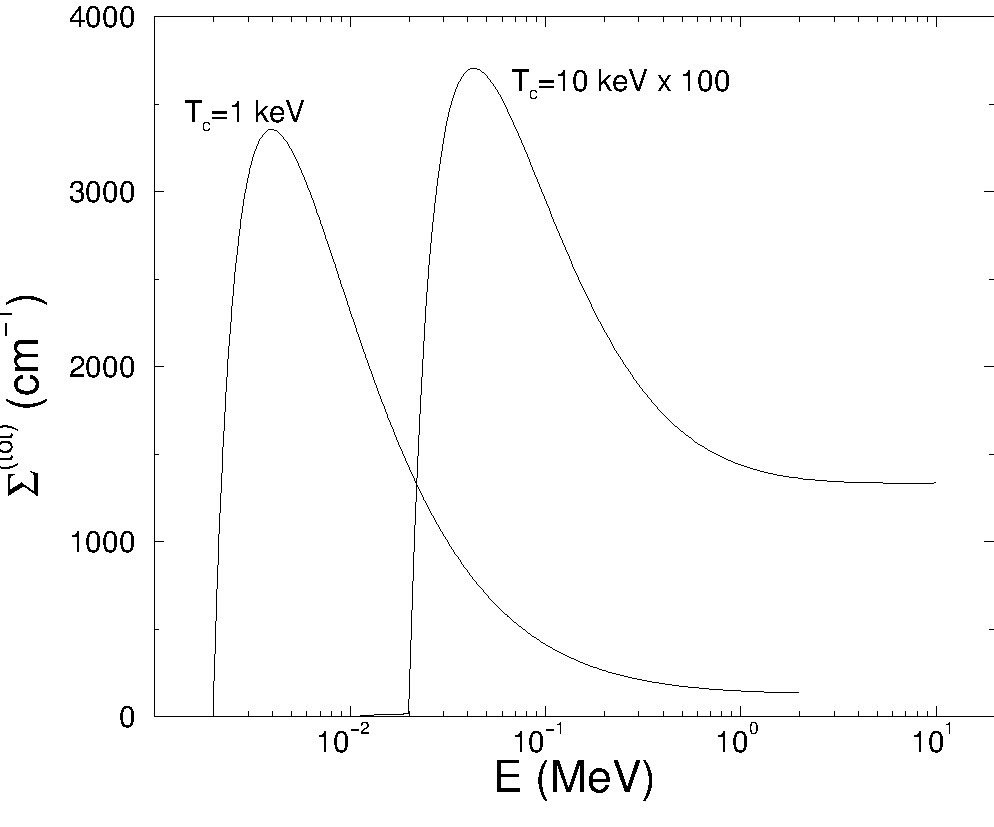
\includegraphics[height=9cm,width=9cm]{figures/cs_all}
\caption[Total discrete interaction cross sections]{\label{sigmas}
The total cross section for
discrete interactions in graphite, calculated with
$T_c = k_c = 1$~keV and $T_c = k_c = 10$~keV
(scaled by a factor of 100) as a function of kinetic energy.}
\end{figure}

In EGSnrc the distance between discrete interactions is measured
in units of the energy loss due to sub-threshold processes.
The relevant total cross section is then
$\tilde{\Sigma}^{\rm (tot)}(E) = \Sigma^{\rm (tot)}(E)/L(E)$
(see the general discussion
of the transport equation in section \ref{electron_general}).
This cross section, shown in Fig. \ref{tilde_sigma} for graphite and gold
for two different values of $T_c$ and $k_c$,
is much flatter than $\Sigma^{\rm (tot)}$
(at least for low cutoff energies)
\begin{figure}[htp]
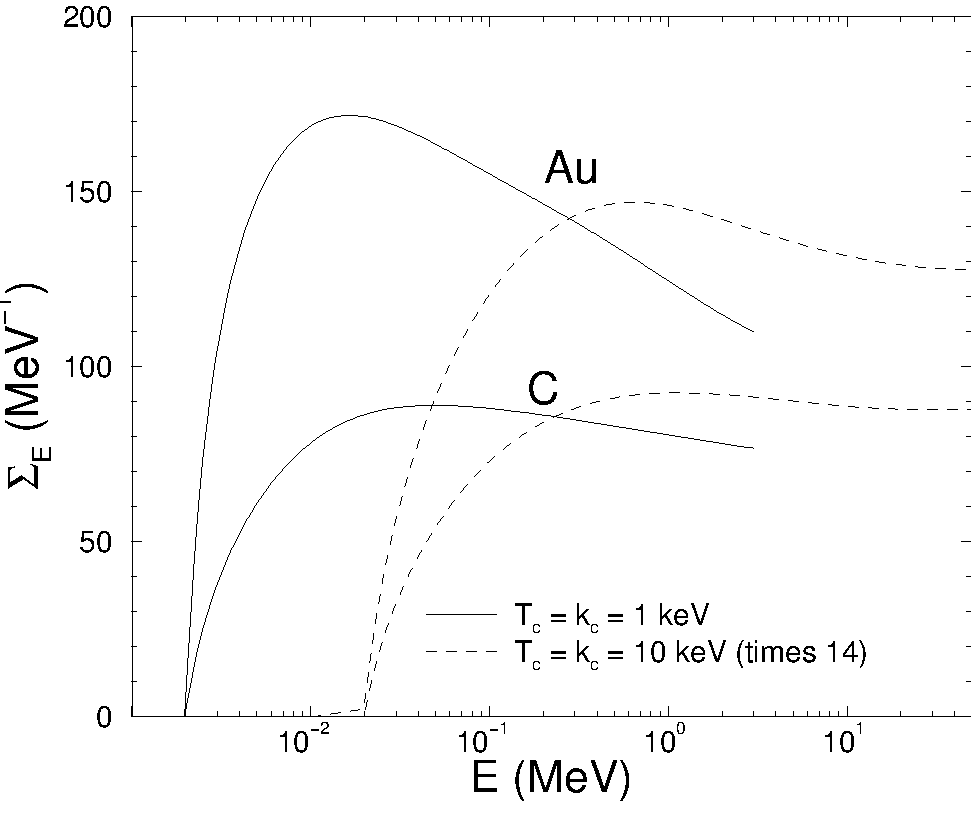
\includegraphics[height=10cm,width=10cm]{figures/cse_all}
\caption[Total cross sections per unit energy loss]{\label{tilde_sigma}
The total cross section
per unit energy loss, $\tilde{\Sigma}^{\rm (tot)}(E)$, for
discrete interactions in graphite and gold, calculated with
$T_c = k_c = 1$~keV and $T_c = k_c = 10$~keV
(scaled with a factor of 14 for better visibility)
as a function of kinetic energy.}
\end{figure}
and has a single maximum. This maximum is determined after
the PEGS data becomes available and is used at run time to
sample energy losses between discrete interactions.
This saves the necessity of evaluating the cross section
at the beginning of each discrete interaction loop
(the {\tt TSTEP LOOP}) in subroutine {\tt ELECTR}.
The procedure described above
is then used to compute the corresponding path-length.

\paragraph{Transport in electromagnetic fields} \hfill
\label{EMF_macros_algorithm}

Transport of charged particles through matter under the influence of electric and magnetic fields is now possible
using the approach proposed by Bielajew\cite{Bi89a}. In this approach, charged particles are forced
to take small enough steps so that the external fields do not change significantly, and energy losses as well
as angular deflections are negligible. Under these assumptions the effect of the electromagnetic field can
be superimposed upon the field-free transport, and the final direction calculated to first order as

\begin{equation}
\Delta\vec{u} = \Delta\vec{u}_{ms,ret} + \Delta\vec{u}_{em}
\end{equation}
where $\Delta\vec{u}_{ms,ret}$ is the angular deflection due to elastic and inelastic scattering which
can be calculated using EGSnrc's electron transport algorithm, and $\Delta\vec{u}_{em}$ is the angular
deflection due to the electromagnetic field, which, to first order, can be obtained from

\begin{equation}
\label{uchange_emf}
    \Delta\vec{u}_{em} = \frac{q \cdot s}{m_0 \gamma v^2_0} \left[\vec{E}_0 - \vec{u}_0(\vec{u}_0\cdot \vec{E}_0) + \vec{v}_0 \times \vec{B}_0\right].
\end{equation}

The final position can be obtained using

\begin{equation}
    \vec{x}_f = \vec{x}_0 + \vec{u}_0 s + \frac{s}{2} \left(\Delta\vec{u}_{ms,ret} + \Delta\vec{u}_{em}\right).
\end{equation}

In the current implementation, lateral displacement due to the Lorentz force is ignored,
and only a condensed history (CH) step $s$ is taken along $\vec{u}_0$ using EGSnrc's electron
transport algorithm. This simplification relies on the assumption that accounting only for
the change in direction due to the Lorentz force is accurate enough when using very small steps.

There are several criteria to restrict the step size based on energy loss, change
in the electromagnetic field and change in particle direction. In the case of a static
$\vec{B}$ field ($\vec{E}$ = 0, $\vec{B}$ = $\vec{B}_0$) only the restriction of small changes
in the particle direction is relevant. According to Eq.(\ref{uchange_emf}), $|\Delta\vec{u}_{em}|$
should only be allowed to take a value $\delta \ll 1$ from where the restricted step size follows as
\begin{equation}
\label{uchange_restriction}
  s = \delta \cdot \frac{E_o \gamma_0 \beta^2}{q\left|\vec{v}_0 \times \vec{B}_0\right|} = \delta \cdot r_g
\end{equation}
the quantity $r_g$ is the well known gyroradius of the particle's trajectory. A value of $\delta$ = 0.02
was used to reproduce the analytical trajectory of electrons in vacuum in reference \cite{Bi89a}.
For more details on the implementation of this algorithm the reader is encouraged to read the very detailed
chapter on this topic by Bielajew\cite{Bi89a}. For instructions on how to enable transport under electromagnetic
fields please refer to section \ref{EMF_macros_implementation}.

\newpage


%%%%%%%%%%%%%%%%%%%%%%%%%%%%%%%%%%%%%%%%%%%%%%%%%%%%%%%%%%%%%%%%%%%%%%%%

%		EGSnrc User Manual

%%%%%%%%%%%%%%%%%%%%%%%%%%%%%%%%%%%%%%%%%%%%%%%%%%%%%%%%%%%%%%%%%%%%%%%%

%\mbox{}\newpage
\renewcommand{\leftmark}{{3: EGSnrc Reference Manual}}
\typeout{Starting ``EGSnrc Reference Manual''  Should be odd page}
%\renewcommand{\rightmark}{{EGSnrc Reference Manual}}

%%%%%%%%%%%%%%%%%%%%%%%%%%%%%%%%%%%%%%%%%%%%%%%%%%%%%%%%%%%%%%%%%%%%%%%%%%%%%%%
%
%  EGSnrc manual: changes from EGS4
%  Copyright (C) 2015 National Research Council Canada
%
%  This file is part of EGSnrc.
%
%  EGSnrc is free software: you can redistribute it and/or modify it under
%  the terms of the GNU Affero General Public License as published by the
%  Free Software Foundation, either version 3 of the License, or (at your
%  option) any later version.
%
%  EGSnrc is distributed in the hope that it will be useful, but WITHOUT ANY
%  WARRANTY; without even the implied warranty of MERCHANTABILITY or FITNESS
%  FOR A PARTICULAR PURPOSE.  See the GNU Affero General Public License for
%  more details.
%
%  You should have received a copy of the GNU Affero General Public License
%  along with EGSnrc. If not, see <http://www.gnu.org/licenses/>.
%
%%%%%%%%%%%%%%%%%%%%%%%%%%%%%%%%%%%%%%%%%%%%%%%%%%%%%%%%%%%%%%%%%%%%%%%%%%%%%%%
%
%  Author:          Iwan Kawrakow, 2003
%
%  Contributors:    Blake Walters
%                   Frederic Tessier
%                   Ernesto Mainegra-Hing
%
%%%%%%%%%%%%%%%%%%%%%%%%%%%%%%%%%%%%%%%%%%%%%%%%%%%%%%%%%%%%%%%%%%%%%%%%%%%%%%%


% Replace line with fixed date with the one below when commiting
% Beware: Using the macro below conflicts between CVS and latex!!!
% \lfoot[{\sffamily {\leftmark}}]{{\small Last edited $Date: 2013/01/04 14:38:47 $
\lfoot[{\sffamily {\leftmark}}]{{\small Last edited 2011/03/09 19:35:20
}}
\newpage

\section{EGSnrc Reference Manual}
\label{ERM}

\subsection{Introduction}

This section is based on Appendix 2 of SLAC-265\cite{Ne85} but
substantially updated and changed to represent the EGSnrc system rather
than EGS4. There have been minor modifications to reflect the EGSnrcMP
environment but these are described more fully in PIRS-877\cite{Ka03}.

\subsubsection{Use of Mortran3}
\index{Mortran3}

Starting with EGS2, the EGS Code System has been written in an extended
Fortran language known as Mortran\cite{Co83}. Section~\ref{UGM3} (page
~\pageref{UGM3}) presents a
brief overview of the elements of Mortran3 which are needed for users of
EGS.

Mortran is a very powerful pre-processor which was ahead of its time back
in the 70's and 80's.  Today many of its features are available in other
languages. Nonetheless we have continued to use Mortran3 because there
are so many user codes available in Mortran3 that it makes no sense to
abandon it.  It is also a very structured language which allows for easy
in-line documentation.


      Although there might be some resistance by users of EGS
 to learn another language, we would like to point out two facts:
\begin{itemize}
      \item   The Mortran language (excluding macros) is trivial
            to learn by those who program in Fortran.

      \item   EGS can be set-up and run by writing entirely in
            Fortran or some other language should the user so desire.
\end{itemize}

 We would encourage EGS users not to do the latter, however, for this
would truly defeat the real purpose for using Mortran---namely, the
macro facility.


\subsection{ General Description of Implementation}
\index{overview of code system}
\index{general description of code system}

The EGS code itself consists of two User-Callable subroutines, {\tt HATCH}
and {\tt SHOWER}, which in turn call the other subroutines in the EGS
code, some of which call three User- written subroutines, {\tt HOWFAR},
{\tt HOWNEAR} and {\tt AUSGAB}.  This is best illustrated with the aid
of Fig.~\ref{fig_egsnrc_structure}

\begin{figure}[hbtp]
\index{schematic of code system}
   \begin{center}
   \leavevmode
   \mbox{}\hspace{-1mm}
   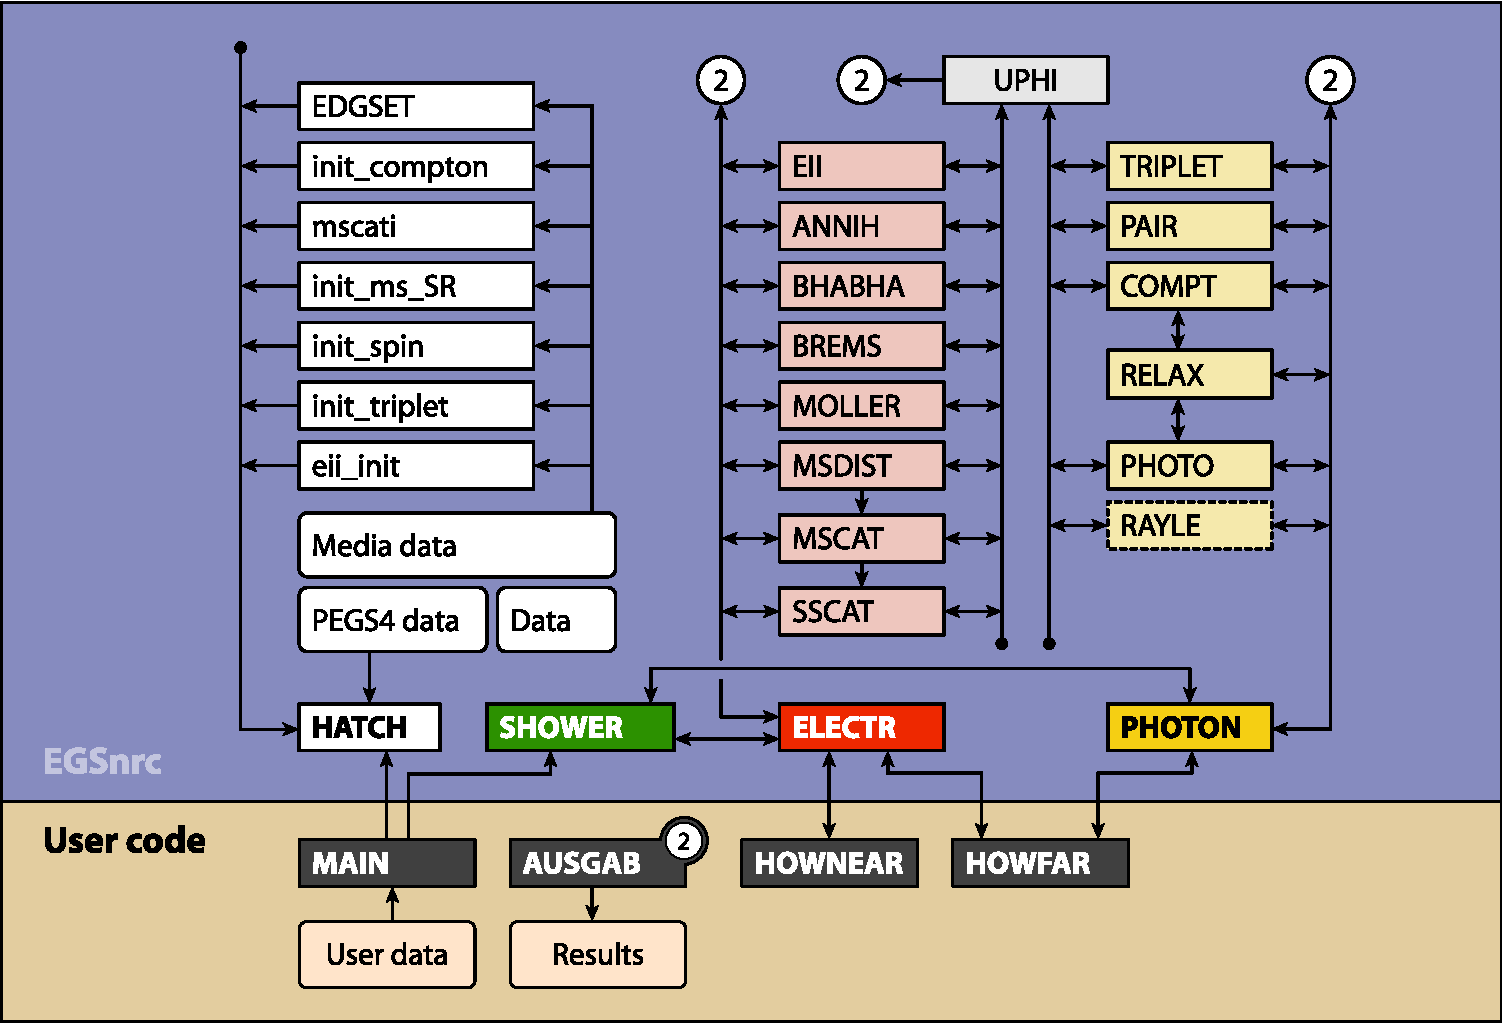
\includegraphics[width=16cm]{figures/egs-diagram}
   \end{center}
   \caption{The structure of the EGSnrc code system when used with a
user-code.}
   \label{fig_egsnrc_structure}
\end{figure}

To use EGS the user must write a ``User Code."  This consists of a
MAIN program and the subroutines {\tt HOWFAR}, {\tt HOWNEAR} and {\tt
AUSGAB}, the latter three determining the geometry and output (scoring),
respectively.  Additional auxiliary subprograms might be included in the
User Code to facilitate matters.  The user can communicate with EGS by
means of various {\tt COMMON} variables.  Usually MAIN will perform
any initialisation needed for the geometry routines, {\tt HOWFAR}
and {\tt HOWNEAR}, and sets the values of certain EGS {\tt COMMON}
variables which specify such things as names of the media to be used,
the desired cutoff energies, and the distance unit to be used (e.g.,
inches, centimeters, radiation lengths, etc.).  MAIN then calls the
{\tt HATCH} subroutine which ``hatches EGS" by doing necessary once-only
initialisation and by reading material data for the media from a data set
that had been previously created by PEGS.  This initialisation completed,
MAIN may then call {\tt SHOWER} when desired.  Each call to {\tt SHOWER}
results in the generation of one history (often referred to as a ``case").
The arguments to {\tt SHOWER} specify the parameters of the incident
particle initiating the cascade.

In addition, macro definitions can be included in MAIN in order to control
or over-ride various functions in EGS as well as in the User-Written
codes.

\index{defaults}
In EGSnrc there are many new options compared to EGS4.  The system
defaults to a set of options which will do the most complete and accurate
simulation that EGSnrc is capable of. In some cases this will imply
overkill and a reduction in efficiency with no gain in accuracy (e.g.
including atomic relaxation or bound Compton scattering for high energy
photon calculations). The user has the ability to switch things on or off
by setting various  flags.  So, eg, one could decide to run a calculation
which is nearly equivalent to using the EGS4/PRESTA electron transport
algorithm (see section~\ref{mimic}). Similarly one can choose to model
Klein Nishina Compton scattering instead of bound compton scattering by
setting a flag.

One other class of new features in EGSnrc is the implementation within the
code itself of several variance reduction techniques (range rejection and
bremsstrahlung splitting being the main two) since by doing so, a much more
efficient implementation is allowed. The user can, of course, completely
ignore these features if so desired.


      In summary, the user communicates with EGS by means of:
\begin{description}
\item[Subroutines]\mbox{}
\begin{itemize}
\item HATCH  --- to establish media data

\item SHOWER --- to initiate the cascade

\item HOWFAR\& HOWNEAR --- to specify the geometry

\item AUSGAB --- to score and output the results and to control variance
reduction

\end{itemize}

\item[COMMON blocks]  by changing values of variables

\item[Macro definitions] --- re-definition of pre-defined features.
\end{description}

To reiterate, we shall refer to the MAIN/HOWFAR/AUSGAB combination
(plus auxiliary subprograms and macros) as the User Code.  The following
sections discuss these things in greater detail.

\clearpage

%\newpage
\subsection{ The COMMON Blocks}

\label{common_blocks} \index{COMMON BLOCKS}
Listed here are the {\tt COMMON} blocks relevant to the user (and
relevant variables contained in them) with a brief description of their
functions.  Their usage will be discussed in more detail in subsequent
sections.  The easiest way to declare any of the {\tt COMMON} blocks is with
the {\tt COMIN} macro.  For example, {\tt COMIN/STACK,BOUNDS/;} will automatically
expand to the correct {\tt COMMON/STACK/;} and {\tt COMMON/BOUNDS/;} forms.

Note that EGSnrc is, by default, coded completely using IMPLICIT NONE. This
means that all parameters in {\tt COMMON} are all explicitly typed. See
section~\ref{implicit_none}  for more info.

\begin{table}[htb]
   \index{BOUNDS} \index{COMMON!BOUNDS} \index{ECUT}
   \index{PCUT} \index{VACDST} \index{EGS-VARIANCE-REDUCTION}
   \index{COMMON!EGS-VARIANCE-REDUCTION} \index{e\_max\_rr} \index{i\_do\_rr}
   \index{i\_play\_RR} \index{i\_survived\_RR} \index{prob\_RR}
   \index{n\_RR\_warning} \index{nbr\_split} \index{bremsstrahlung!splitting}
   \index{Russian Roulette} \index{range rejection}
   \index{bound Compton scattering}

\typeout{starting common BOUNDS table }


\begin{center}
\caption{Table describing the EGSnrc {\tt COMMON}s which are accessible to the
User.
\label{tab_commons}
}
\begin{tabular}{ l l   p{105mm}l  |}
\hline
Common & Variable & Description \\
Block &&\\
\hline
&&\\
{\bfseries BOUNDS} & ECUT &Array of regions' charged particle
                            cutoff energies(total) in MeV.\\
       & PCUT &Array of regions' photon cutoff
                            energies in MeV.\\
       & VACDST  &   Distance to transport in vacuum (default=1.E8).\\
&&\\
\hline
&&\\
\multicolumn{3}{l}{{\bfseries EGS-VARIANCE-REDUCTION}}\\
	&e\_max\_rr &real array (\$MXREG) of maximum total energies at which
                     to do range rejection if i\_do\_rr is set\\
	&i\_do\_rr &integer array (\$MXREG) of flags for range rejection
                    in each region. ~~~~0$\Rightarrow$ not done (default);
                      ~~~~1$\Rightarrow$ is done.\\
&&\\
	& i\_play\_RR & flag specifying if Russian Roulette played on a
                        global basis\\
        & i\_survived\_RR & an integer flag set every time Russian Roulette
is played. If all the particles survive, it is set to 0 (which is the default
if not played at all). It is set to n if n particles were eliminated via
Russian Roulette on this interaction. It is 0 if a bound compton event is
rejected.\\
&&\\
	& prob\_RR & probability of survival if playing Russian Roulette\\
	& n\_RR\_warning & an internal counter to mark how often Russian
	Roulette is asked for with prob\_RR $\le$ 0.0. A warning is printed
       for the first \$MAX-RR-WARNING times (default 50).\\
&&\\
	&nbr\_split& For nbr\_split $>$1, nbr\_split brems photons are
sampled {every time} there is a brem interaction. The weight is reduced by
1/nbr\_split. Default value is 1.0.  If set to zero, no brem is generated
and the electron loses no energy.\\
%&&\\
\hline
    \end{tabular}
    \end{center}
    \mbox{}\hfill (cont ...)\\
    \end{table}
    \clearpage

\begin{table}[htb]
   \index{EPCONT} \index{COMMON!EPCONT} \index{EDEP} \index{TSTEP}
   \index{TUSTEP} \index{USTEP} \index{VSTEP} \index{IDISC} \index{IROLD}
   \index{IRNEW} \index{EOLD} \index{RHOF} \index{ENEW} \index{BETA2}
   \index{IAUSFL} \index{EKE} \index{ELKE} \index{GLE} \index{E\_RANGE}

\typeout{starting next common EPCONT table }
    \begin{center}
    EGSnrc COMMONs which are accessible to the User -continued\vspace*{3mm}
    \begin{tabular}{ l  l   p{105mm}l  |}
    \hline
    Common & Variable & Description \\
    Block &&\\
    \hline
&&\\
{\bfseries EPCONT}  & EDEP & Energy deposited in MeV (Double
                            Precision).\\
        & TSTEP  & Distance to next interaction (cm)\\
        & TUSTEP  & Total (curved) step length requested before check with
		geometry.\\
	& USTEP	& straight step length calculated from TUSTEP.\\
        & TVSTEP & Actual total (curved) step length to be transported.\\
	& VSTEP	& actual straight step length after truncation by geometry.\\
        & IDISC  & User discard request flag (to be set in {\tt HOWFAR}).
                   IDISC $>$ 0 means user requests immediate discard,
                   IDISC $<$ 0 means user requests discard after completion
                   of transport, and IDISC=0 (default) means no user
                   discard requested. IDISC=99 or $-$99 means generate
		   annihilation photons when positron is discarded.\\
         &IROLD  &Index of previous region.\\
         & IRNEW  & Index of new region.\\
         & RHOF   & Value of density correction (default=1) (i.e. ratio
                    of real density to that of dataset.\\
         & EOLD   &  Charged particle (total) energy
                            at beginning of step in MeV.\\
           & ENEW   & Charged particle (total) energy
                            at end of step in MeV.\\
           %& BETA2 & Beta squared for present particle.
                  %          (Note: BETA is not included).\\

           & IAUSFL & Array(35) of flags for turning on
                   various calls to {\tt AUSGAB}. See table~\ref{tab_iausflg_other}\\
           & EKE   & Electron kinetic energy in MeV.\\
           & ELKE  & Natural logarithm of EKE (this is not available for
                     a step in vacuum).\\
           & GLE   & Natural logarithm of photon energy.\\
           & E\_RANGE & For electron {\tt IARG}=0  steps, this is the range of the
electron in the current units (see section~\ref{range_rejection}).\\
           & x[y][z]\_final & position at end of step \\
           & u[v][w]\_final & direction at end of step (only used for electrons)\\
&&\\
\hline
    \end{tabular}
    Note: the variable BETA2 is no longer available.\\
    \end{center}
    \mbox{}\hfill (cont ...)\\
    \end{table}

\clearpage

  \begin{table}[htb]
   \index{ET-Control} \index{COMMON!ET-Control} \index{SMAXIR}
   \index{ESTEPE} \index{XIMAX} \index{SKINDEPTH\_FOR\_BCA}
   \index{TRANSPORT\_ALGORITHM} \index{SPIN\_EFFECTS} \index{EGS4}
   \typeout{starting next common ET-Control table }
   \index{BCA\_ALGORITHM}
    \begin{center}
    EGSnrc COMMONs which are accessible to the User -contnued\vspace*{3mm}
    \begin{tabular}{ l  l   p{105mm}l  |}
    \hline
    Common & Variable & Description \\
    Block &&\\
    \hline
    &&\\
    \multicolumn{2}{l}{{\bfseries ET-Control}}  &  Electron Transport Control.\\
    &&\\
	&SMAXIR	&array(\$MXREG) defining upper limit on step size in each
		region (in whatever units defined by DUNIT).(default=1.E10).\\
    &&\\
	&ESTEPE	&global energy loss constraint.(default=0.25).\\
    &&\\
	&XIMAX	&max. first GS moment per step (roughly half the average
                MS angle squared.(default 0.5).\\
    &&\\
	&SKINDEPTH      & distance from a boundary (in elastic MFP) at which to\\
	&  ~~~\_FOR\_BCA& switch to one of the boundary crossing
		  algorithms(BCAs).(default 3).  If set 0 by the user
                  initially and BCA\_ALGORITHM = 1, then the code assigns
                  a value consistent with
                  BLCMIN in PRESTA-I, otherwise it is 3.0.\\
    &&\\
	&TRANSPORT& integer flag telling which transport algorithm to use.\\
 	& \_ALGORITHM	& 0$\Rightarrow$ PRESTA-II; 1$\Rightarrow$
                    PRESTA-I.(default 0).\\
    &&\\
	&BCA	&integer flag telling which BCA to use. \\
	&\_ALGORITHM  & 0$\Rightarrow$ use exact(single scattering) algorithm
                         within SKINDEPTH\_FOR\_BCA of a boundary\\

        &            &  1$\Rightarrow$ use multiple scattering but with
                  no lateral deflections within SKINDEPTH\_FOR\_BCA of a
                  boundary.  Default is  0.\\
    &&\\
      	&SPIN &logical variable, {\tt .true.}$\Rightarrow$ use single \&
                multiple scattering\\
	&\_EFFECTS	& theories which include relativistic spin
               effects; {\tt .false.}
		$\Rightarrow$ use single and multiple scattering theories
                based on Rutherford scattering. (default {\tt .true.})\\
%to be closer to EGS4).\\
	&&\\
   \hline
   \end{tabular}
   \end{center}
\end{table}

\clearpage

\begin{table}[htb]
    \index{MEDIA} \index{COMMON!MEDIA} \index{NMED} \index{IRAYLM} \index{RLC}
    \index{RLDU} \index{RHO}
    \index{MISC} \index{COMMON!MISC} \index{MED} \index{DUNIT} \index{KMPI}
    \index{KMPO} \index{RHOR} \index{NOSCAT} \index{IRAYLR}
    \index{RANDOM} \index{COMMON!RANDOM} \index{IXX} \index{JXX}
    \index{random number generators!seeds} \index{RANMAR} \index{RANLUX}

\typeout{****start Common MEDIA}
    \begin{center}
    EGSnrc COMMONs which are accessible to the User (cont)\vspace*{2mm}
    \begin{tabular}{ l  l   p{105mm}l  |}
    \hline
    Common & Variable & Description \\
    Block &&\\
    \hline
&&\\
{\bfseries MEDIA}	& MEDIA	&array(24,\$MXMED)  of media names.\\
	& NMED	& Number of media being used
                            (default=1).\\
          & IRAYLM & Array(\$MXMED) of flags for turning on (=1)
                            coherent (Rayleigh) scattering in
                            various media.  Set in {\tt HATCH} based
                            on values of IRAYLR.  \\
          & RLC   & Array(\$MXMED) containing radiation
                            lengths of the media in cm.  \\
	& RLDU  &  Array(\$MXMED) containing radiation
                            lengths of the media in distance
                            units established by DUNIT.\\
	&RHO	& Array(\$MXMED) containing density of the
                            media in g/cm**3.\\
        &MGE    & Array(\$MXMED) number of photon mapped energy intervals for
                  a given medium.\\
        &MEKE   & Array(\$MXMED) nuber of electron mapped energy intervals for
                  a given medium.\\
       &comp\_xsections & character*16 variable holding the name of the file\\
       && containing user-supplied Compton cross section data.\\
       &&  Full name of the file is\\
       && {\tt \$HEN\_HOUSE/data/comp\_xsections\_compton.data}.\\
       && Only used if {\tt IBCMP}=2 (bound Compton, no doppler effect).\\
&&\\
\hline
&&\\
{\bfseries MISC$^*$}	& MED	&Array(\$MXREG) containing medium index for
                            each region.\\
	& DUNIT	&The distance unit to be used.
                            DUNIT=1 (default) establishes all
                            distances in cm; whereas,
                            DUNIT=2.54 establishes all
                            distances in inches.\\
	&KMPI	&Fortran unit number (default=12)
                            from which to read material data.\\
	&KMPO	&Fortran unit number (default=8) on
                            which to ``echo" material data (e.g.,
                            printed output, ``dummy" output, etc.).\\
	&RHOR	&Array(\$MXREG) containing the density for each region (g/cm**3).
		If this is different than the default density for the medium
		for that region, the cross sections and stopping powers (with
		the exception of the density effect) are scaled appropriately.\\
	%&NOSCAT&Number of times multiple scattering has been bypassed in
        %       subroutine MSCAT (initialized to 0 in BLOCK DATA). This
	%       applies only if PRESTA-I or EGS4 options being used since
        %       it is never turned off in default EGSnrc.\\
	&IRAYLR	&Array(\$MXREG) of flags for turning on (=1)
                            coherent (Rayleigh) scattering in
                            various regions (default=0$\Rightarrow$ off).\\
&&\\
\hline
\multicolumn{3}{c}{$^*$ NOSCAT is no longer available since there is
scattering on all steps.}\\
&&\\
%this common block is now found in ranmar.macros and ranlux.macros and,
%moreover, does not include ixx, jxx
%{\bfseries RANDOM}
%	&IXX,JXX & When using the RANLUX random number generator, the user
%does not pass anything via this {\tt COMIN}. When using RANMAR, IXX and JXX
%are passed. Initially random number seeds, these
%become pointers once the generator is initialized. 0$<$IXX$<=$31328 and 0$<$JXX$<=$30081.\\
\hline
    \end{tabular}
    \end{center}
    \mbox{}\hfill (cont ...)\\
    \end{table}
    \clearpage



\begin{table}[htb]

   \index{STACK} \index{COMMON!STACK} \index{E} \index{X,Y,Z} \index{U,V,W}
   \index{DNEAR} \index{WT} \index{IQ} \index{IR} \index{NP} \index{NPold}
   \index{LATCH} \index{LATCHI}


   \index{THRESH} \index{COMMON!THRESH} \index{RMT2} \index{RMSQ} \index{AP}
   \index{UP} \index{AE} \index{UE} \index{TE} \index{THMOLL} \index{\$MXMED}
   \index{\$MXSTACK} \index{variance reduction}

\typeout{****start COMMON STACK}

    \begin{center}
    EGSnrc COMMONs which are accessible to the User (cont).
    \begin{tabular}{ l  l   p{105mm}l  |}
    \hline
    Common & Variable & Description \\
    Block &&\\
    \hline
&&\\
{\bfseries STACK}	&	&Note: This COMMON block contains the
                            information about the particles
                            currently in the shower.  All
                            of the following variables are
                            arrays(\$MXSTACK) except {\tt NP, NPold}  and
                            {\tt LATCHI}.\\
	&E	&Total energy in MeV (Double
                            Precision).\\
	& X,Y,Z & Position of particle in units
                            established by DUNIT.\\
	&U,V,W	&Direction cosines of particle (not
                            necessarily normalized if table lookups used
                      for sines---see section~\ref{step_1}).\\
	&DNEAR	&A lower bound of distance from
                            (X,Y,Z) to nearest surface of
                            current region.\\
	& WT	&Statistical weight of current particle(default=1.0).  To be
		used in conjunction with variance reduction techniques as
                determined by user.\\
	& IQ	&Integer charge of particle
                            (+1,0,-1).\\
	&IR	&Index of particle's current region.\\

	& NP	& The stack pointer (i.e., the particle currently being pointed
                            to).  Also, the number of particles on the stack.\\

	&NPold	& Value of {\tt NP} prior to an interaction (to test how many
		particles created see section~\ref{stack_status}).\\

	&LATCH	&An integer variable for use to track histories.\\

	&LATCHI	&Initial value of LATCH(1) when shower called.\\
&&\\
\hline
&&\\
{\bfseries THRESH}	&RMT2	&Twice the electron rest mass
                            energy in MeV.\\
	&RMSQ	& Electron rest mass energy squared
                            in MeV-squared.\\
	&AP	&Array(\$MXMED) containing PEGS lower photon
                            cutoff energy for each medium in
                            MeV.\\
	&UP	& Array(\$MXMED) containing PEGS upper photon
                            cutoff energy for each medium in
                            MeV.\\
	&AE	&Array(\$MXMED) containing PEGS lower charged
                            particle cutoff energy for each
                            medium in MeV.\\
	&UE	&Array(\$MXMED) containing PEGS lower charged
                            particle cutoff energy for each
                            medium in MeV.\\
	&TE	&Same as AE except kinetic energy
                            rather than total energy.\\
	&THMOLL	&Array(\$MXMED) containing the Moller thresh-
                            hold energy (THMOLL=AE+TE) for
                            each medium in MeV.\\
&&\\
\hline
    \end{tabular}
    \end{center}
    \mbox{}\hfill (cont ...)\\
    \end{table}
    \clearpage

\begin{table}[htb]
   \index{UPHIOT} \index{COMMON!UPHIOT} \index{THETA} \index{SINTHE}
   \index{COSTHE} \index{SINPHI} \index{COSPHI} \index{PI} \index{TWOPI}

   \index{USEFUL} \index{COMMON!USEFUL} \index{MEDIUM} \index{MEDOLD}
   \index{RM} \index{PRM} \index{PRMT2} \index{PZERO}
   \index{USER} \index{COMMON!USER}

    \begin{center}
    EGSnrc COMMONs which are accessible to the User (cont).
    \begin{tabular}{ l  l   p{105mm}l  |}
    \hline
    Common & Variable & Description \\
    Block &&\\
    \hline
    &&\\
    {\bfseries UPHIOT}	&THETA	&Collision scattering angle (polar).\\
	&SINTHE	& Sine of THETA.\\
	&COSTHE & Cosine of THETA.\\
	&SINPHI	&Sine of PHI (the azimuthal
                            scattering angle of the collision).\\
	&COSPHI	& Cosine of PHI.\\
	&PI	& Pi.\\
	&TWOPI	& two Pi.\\
        &PI5D2  & 2.5 $\times$ Pi.\\
    &&\\
    \hline
    &&\\
    {\bfseries USEFUL}	&MEDIUM	&Index of current medium.  If
                            vacuum, then MEDIUM=0.\\
	&MEDOLD	&Index of previous medium.\\
	&RM	&Electron rest mass energy in MeV.(see also THRESH)\\
	&PRM	& ``Precision" electron rest mass
                            energy in MeV (Double Precision).\\
	&PRMT2	&Twice PRM (Double Precision).\\
	&PZERO	&precise 0.0 (Double Precision).\\
    &&\\
   \hline
    &&\\
    {\bfseries USER} & & Null by default but available in ELECTR, PHOTON
                     and HATCH to allow users to pass data into the
        transport routines (eg geometry data, variance reduction data
etc).\\
    &&\\
   \hline
&&\\
{\bfseries CH-Steps} & {\tt count\_pII\_steps} & keeps a count of number of
electron steps taken using the PRESTA-II multiple scattering model
(real*8).\\
& {\tt count\_all\_steps} & counts all electron steps (real*8).\\
& {\tt is\_ch\_step} & a logical variable set to true if the current electron\\
&& step is a condensed history ({\em i.e.} using PRESTA-I or PRESTA-II multiple\\
&& scattering theory) step.\\
&&\\
   \end{tabular}
   \end{center}
\end{table}

\clearpage

As well as the {\tt COMIN}s described above, there are several {\tt COMIN}s which are
normally just internal to EGSnrc, which have one or two variables which the
user may require access to in order to control various options within
 EGSnrc.  In an ideal world these would all be gathered into a single
{\tt COMIN}
but that would make compatibility with EGS4 user codes even more difficult
to achieve.  We have adopted this compromise solution which changes as
little as possible of what has grown up historically with EGS4.  So, for
example the parameters {\tt IEDGFL}, {\tt IPHTER},
{\tt IBRDST} and {\tt IPRDST} have not been
moved and the new parameters introduced with EGSnrc have similarly been
placed in those {\tt COMIN}s associated with the physics being controlled.
Table~\ref{tab_new_commons} summarizes these {\tt COMIN}s which are needed to
control further the transport parameters.  Note that the user code can
ignore these {\tt COMIN}s completely if you are satisfied with the default
settings for photon and electron transport in EGSnrc.
\index{EGS4}
\index{IPRDST} \index{IBRDST}
\clearpage

\clearpage
 \begin{table}[hb]
\index{COMINs}
\index{ibr\_nist}
\index{EDGE}
\index{COMMON!EDGE}
\index{IEDGFL}
\index{IPHTER}
\index{photoelectric interactions}
\index{fluorescence}
\index{photoelectric interactions!angular distribution}
\index{COMMON!COMPTON-DATA}
\index{COMPTON-DATA}
\index{Compton effect}
\index{bound Compton scattering}
\index{Doppler effects}
\index{IBCMP}
\index{BREMPR}
\index{COMMON!BREMPR}
\index{IBRDST}
\index{IPRDST} \index{EGS4}
\index{bremsstrahlung!production}
\index{bremsstrahlung!angle}
\index{pair production}
\index{Coster-Kronig electrons}
\index{Koch and Motz}
\index{RAYLEIGH\_INPUTS}
 \begin{center}
 \label{tab_new_commons}
 \caption{EGSnrc {\tt COMMON}s which are optionally accessible to the user. Not all
elements in each {\tt COMIN} are described since many of them are not
to be accessed by the user.\vspace*{5mm} }
 \begin{tabular}{ l  l   p{105mm}l  |}
 \hline
 Common & Variable & Description \\
  Block &&\\
    \hline
&&\\
{\bfseries EDGE}	&IEDGFL	& integer array (\$MXREG) specifying whether
relaxation of the atom is modelled after photo-effect or bound compton
events (at present). When on, fluorescent photons, Auger electrons and
Coster-Kronig electrons above threshold are modelled explicitly. When not
on, the photoelectron acquires the entire energy of the incident photon
(contrary to what happened in EGS4).  (1$\Rightarrow$ yes (default),
0$\Rightarrow$ no).\\
	&IPHTER	& integer  array (\$MXREG) specifying whether to sample the
         angular distribution of photo-electrons in each region
(1$\Rightarrow$ yes (default),
0$\Rightarrow$ no) .\\
&&\\
% do we want to list more from this common block here
\hline
&&\\
{\bfseries COMPTON-} &IBCMP &integer array (\$MXREG) specifying whether to
                    include \\
{\bfseries ~~~~~~DATA} & & binding and Doppler broadening effects in Compton
            scattering events (1$\Rightarrow$ yes (default), 0$\Rightarrow$ no).\\
                  & radc\_flag & integer flag for radiative Compton corrections.\\
                 && 0$\Rightarrow$ off (default), 1$\Rightarrow$ on.\\
&&\\
\hline
&&\\
{\bfseries BREMPR} &  IBRDST & flag determining how angle of a brem
photon is selected.  0$\Rightarrow$ sample leading term of the angular
dist'n; 1$\Rightarrow$ sample the ang. distn. of Koch and Motz. Default=1.
For $<$0, the angle is the same as that of the photon so user can use a
call to {\tt AUSGAB} to set the angle.\\

& IPRDST &flag determining how the electron/positron angles are selected
after pair production. 0$\Rightarrow$ use the fixed angle approximation of
EGS4. 1$\Rightarrow$ sample the leading term in the angular distribution
(fast and good enough). 2$\Rightarrow$ sample the complete angular distribution.  Default is 1.\\

& ibr\_nist& integer flag determining which differential photon cross section
to sample when brem occurs.\\
&& 0$\Rightarrow$ use Bethe-Heitler as done in EGS4. This is the default.\\
&& 1$\Rightarrow$ use NIST data base from ICRU Report 37.\\
& itriplet & set to 1 to explicitly simulate triplet events (default is 0).\\
& pair\_nrc & flag determining which pair production cross-sections are used.\\
&& 0$\Rightarrow$ use Bethe-Heitler cross-sections (default).\\
&& 1$\Rightarrow$ use NRC cross-sections \\
&&\\
\hline
    \end{tabular}
    \end{center}
    \mbox{}\hfill (cont ...)\\
    \end{table}
    \clearpage

\begin{table}[htb]

   \index{EII-DATA} \index{RAYLEIGH\_INPUTS} \index{EGS-IO}
   \index{electron impact ionization!inputs}
   \index{Rayleigh custom form factors}
    \index{I/O file units}
    \begin{center}
    EGSnrc internal COMMONs optionally accessible to the User (cont).
    \begin{tabular}{ l  l   p{105mm}l  |}
    \hline
    Common & Variable & Description \\
    Block &&\\
    \hline
&&\\
{\bfseries EII-DATA} & {\tt eii\_flag} & flag determining which, if any, electron
impact ionization theory is used.\\
&& 0$\Rightarrow$ turn electron impact ionization off (the default).\\
&& 1$\Rightarrow$ use Kawrakow's EII theory\cite{Ka02b}.\\
&& 2$\Rightarrow$ use the theory of Casnati\cite{Ca82}.\\
&& 3$\Rightarrow$ use the theory of Kolbenstvedt\cite{Gr65a}.\\
&& 4$\Rightarrow$ use the theory of Gryzinski\cite{Ko67}.\\
&&\\
\hline
&&\\
{\bfseries RAYLEIGH} & {\tt iray\_ff\_media} & array (with dimension
{\tt \$MXMED}) containing the names of the\\
{\bfseries \mbox{~~~~}\_INPUTS}&& media (must appear in the PEGS4 data) for which custom Rayleigh
form factors are to be provided.  Otherwise, the medium
uses the default atomic form factor.\\
& {\tt iray\_ff\_file} & array (with dimension {\tt \$MXMED}) containing
full names ({\em} including directory path) of files specifying
custom form factors.  {\tt iray\_ff\_file(i)} corresponds to
{\tt iray\_ff\_media(i)}.\\
&&\\
\hline
&&\\
{\bfseries EGS-IO} & {\tt file\_extensions} & character array (with
dimension {\tt \$mx\_units}; default=20) containing
extensions of files specified in the code's {\tt .io} file.
Maximum extension length is {\tt \$max\_extension\_length} (default=10 characters).\\
& {\tt file\_units} & integer array (with
dimension {\tt \$mx\_units}) where {\tt file\_units(i)} specifies Fortran unit number associated with
the file having extension {\tt file\_extensions(i)}.\\
& {\tt user\_code} & the name of the user code (max. length = 64 chars).\\
& {\tt input\_file} & the name of the input file.  Includes directory path but
no extension (max. length=256 chars).\\
& {\tt output\_file} & same as above but for the output file.\\
& {\tt pegs\_file} & the name of the pegs data file.  Includes directory path
and extension (max. length=256 chars).\\
& {\tt hen\_house} & the user's {\tt \$HEN\_HOUSE} directory (max. length=128 chars).\\
\hline
    \end{tabular}
    \end{center}
    \mbox{}\hfill (cont ...)\\
    \end{table}
    \clearpage

\begin{table}[htb]

   \index{EGS-IO}
   \index{I/O file units}

    \begin{center}
    EGSnrc internal COMMONs optionally accessible to the User (cont).
    \begin{tabular}{ l  l   p{105mm}l  |}
    \hline
    Common & Variable & Description \\
    Block &&\\
    \hline
\hline
{\bfseries EGS-IO} & {\tt egs\_home} & the user's {\tt \$EGS\_HOME} directory (max. length=128 chars).\\
\mbox{~~~}{\bfseries (cont)}& {\tt work\_dir} & the temporary working directory created in the user's
{\tt \$EGS\_HOME/user\_code} during a run (max. length=128 chars).\\
& {\tt host\_name} & the name of the machine being run on (max. length=64 chars).\\
& {\tt n\_parallel} & if $>$0, the total number of parallel jobs.\\
& {\tt i\_parallel} & if $>$0, the number of the current parallel job.\\
& {\tt first\_parallel} & the first parallel job number (default=1).\\
& {\tt n\_max\_parallel} & max. number of parallel jobs executing simultaneously
(updated during run).\\
& {\tt n\_chunk} & no. of histories per calculation chunk during a parallel run.
(currently not used).\\
& {\tt n\_files} & no. of files specified in the {\tt user\_code.io} file
(max={\tt \$mx\_units}).\\
& {\tt i\_input} & unit no. for standard input, or the {\tt .egsinp} file (default=5).
Note this is used in BEAMnrc to prevent unit collisions when used as
a shared library source.\\
& {\tt i\_log} & unit no. for standard output, or the {\tt .egslog} file (default=6).
Used in BEAMnrc to prevent unit collisions when used as a
shared library source.\\
& {\tt i\_incoh} & unit numbers for data files containing Compton (default=78),\\
& {\tt i\_nist\_data} & bremsstrahlung (default=76), multiple scattering (default=11),\\
& {\tt i\_mscat} & photon cross-section (default=79), and photon relaxation\\
& {\tt i\_photo\_cs} & data (default=77), respectively.  Variable unit numbers\\
& {\tt i\_photo\_relax} & are used to allow BEAMnrc shared library sources to
access these files as well.\\
& {\tt xsec\_out} & =0 $\rightarrow$ do not output file {\tt user\_code.xsections} containing photon cross-section data (default).\\
&& =1 $\rightarrow$ output file containing photon cross-section data.\\
& {\tt is\_batch} & logical variable set to {\tt .true.} if this is a batch
job.\\
&&\\
\hline
&&\\
\end{tabular}
\end{center}
\end{table}
\clearpage

\subsection{The Sequence of Operations}
\index{sequence of operations}
\index{steps}
\index{steps!order}

The sequence of operations needed for the correct operation of EGS is
shown below.

\begin{description}
\item[Step 0.]  {\tt call egs\_init} for file initialization (see
PIRS-877 for details\cite{Ka03}).
\item[Step 1.]  User Over Ride Of EGS Macros and Defaults (\ref{step_1})
\item[Step 2.]  Pre-{\tt HATCH} Call Initialisation (\ref{step_2})
\item[Step 3.]  {\tt HATCH} Call (\ref{step_3})
\item[Step 4.]  Initialisation For {\tt HOWFAR} \& {\tt HOWNEAR} (\ref{step_4})
\item[Step 5.]  Initialisation For {\tt AUSGAB} (\ref{step_5})
\item[Step 5b.] Initialisation For Variance Reduction (\ref{step_5b})
\item[Step 6.]  Determination Of Incident Particle Parameters
              (\ref{step_6})
\item[Step 7.]  SHOWER Call (\ref{step_7})
\item[Step 8.]  Output Of Results (\ref{step_8})
\item[Step 9.] {\tt call egs\_finish} as the last executable statement. See
ref~\cite{Ka03} for details. Properly closes files and places them back on
the user-code's directory.
\end{description}
\vspace*{-4mm}
 The following are restrictions on the order of these
 operations:
\vspace*{-4mm}
\begin{enumerate}
\item  Step 1 must precede use of any EGS macros by the user.
\item Step 0 should be the first executable statement and thus is usually
after Step 1 and possibly in Step 2.
\item  Step 2 must precede Step 3.
\item Steps 3 through 6 must precede Step 7.
\item Step 7 may be repeated as often as desired, depending on whether
  information on single showers or many showers is desired (e.g., for shower
  fluctuation or conversion efficiency calculations).
\item At least one Step 7 must precede the first Step 8.
\end{enumerate}

Details for the above steps are given in the following sub-sections.

It is strongly advised that the user echo {\bfseries ALL} input parameters
into the output listing file to ensure that the listing has a complete
record of the run.  From extensive experience we have found that this is
essential and very valuable.


 \subsubsection{User Over Ride Of EGS Macros and Defaults (Step 1)}
\label{step_1}
\index{Step 1: Override macros}

EGS macros which the user might want to over-ride include the following:

\paragraph{{\tt \$CALL-HOWNEAR(\#)}}
\label{hownear_macro}
\index{EGS4}
\mbox{}\\
For compatibility with  EGS4/PRESTA user-codes, the use of {\tt SUBROUTINE
HOWNEAR} has been left as a macro call in EGSnrc.
There is no default definition of the macro but the following is suggested:
\begin{verbatim}
REPLACE {$CALL-HOWNEAR(#);} WITH {CALL HOWNEAR({P1},X(NP),Y(NP),Z(NP),IRL);}
\end{verbatim}
The user may choose to define an equivalent macro.
The parameter that must be returned by the macro
is the shortest distance to any
boundary from the current position. See
section~\ref{hownear}(page~\pageref{hownear}) which
specifies the macro or subroutine completely.  There is also some
discussion in section~\ref{hownear_change} (page~\pageref{hownear_change}).
\index{HOWNEAR}
\index{SUBROUTINE HOWNEAR}
\index{\$CALL-HOWNEAR}

\paragraph{{\tt \$IMPLICIT-NONE, \$REAL, \$INTEGER}}
\label{implicit_none}
\mbox{}\\
The EGSnrc system is now coded with {\tt \$IMPLICIT-NONE;} (which defaults
to {\tt IMPLICIT NONE;}) in all
subroutines. This means that any time the user is passing a variable
into the EGSnrc system by means of adding to a {\tt COMIN} definition, one
must explicitly specify the type of that variable.  To turn this feature off one adds
the following statement to the user code:
\begin{verbatim}
                REPLACE {$IMPLICIT NONE;} WITH {;}
\end{verbatim}
It is strongly recommended that user codes adopt the use of {\tt
\$IMPLICIT NONE;} since it catches many coding errors and prevents
accidental collision of variables.

\index{\$IMPLICIT-NONE}
\index{\$REAL}
\index{\$INTEGER}
\index{IMPLICIT-NONE}
\index{REAL}
\index{INTEGER}

In addition to using {\tt \$IMPLICIT NONE;}, the EGSnrc system has used
the macros {\tt \$REAL} and {\tt \$INTEGER} everywhere to define real
and integer variables as well as using generic intrinsic functions such
as MAX and MIN.  By default {\tt \$REAL} and {\tt \$INTEGER} are defined
as {\tt REAL*8} and {\tt INTEGER*4}.  However, to make the entire code
run in single precision, one can add the macro:
\begin{verbatim}
                REPLACE {$REAL} WITH {;REAL*4}
\end{verbatim}
However, this requires that all type declarations in the user code also use
the macros {\tt \$REAL} and {\tt \$INTEGER} everywhere.  With 64 bit
machines, one might as well use the {\tt REAL*8} default.

\paragraph{Array Dimensions}
\index{\$MXMED}
\index{\$MXREG}
\index{\$MXSTACK}
\begin{description}
\item[{\tt \$MXMED}]   Maximum number of media (default=10).
\item[{\tt \$MXREG}]   Maximum number of regions (default=2000).
\item[{\tt \$MXSTACK}]  Maximum number of particles on the {\tt STACK} at once
(default = 40).
\end{description}
For example, to extend the number of media to 25, include the following
statement in the User Code.
\begin{verbatim}
         REPLACE {$MXMED} with {25}
\end{verbatim}
Note that there are often array dimensions defined by the user for scoring
arrays and these should be defined at this step as well.

\paragraph{Random Number Initialisation}
\label{rng_init}

\index{random number generators!initialisation}
\index{\$INITIALIZE RNG USING} \index{luxury level} \index{iseed}
\index{RANMAR} \index{RANLUX}
\mbox{}\\
By default the RANLUX random number generator requires no
initialisation. However, to use a luxury level different from the default
of 1,  or a different initial seed, then you must initialize it using:
\begin{verbatim}
         $INITIALIZE RNG USING luxury_level AND iseed;
\end{verbatim}
The {\tt luxury levels} are from 0 to 4, but the value 0 is known to cause
problems with EGSnrc calculations. The value of {\tt iseed} is from 1 to
1073741824 (2$^{30}$).

If you have selected the RANMAR random number generator (via the {\tt
.configuration} file, then it MUST be initialized before it is first used.
This can be accomplished by including the statement:
\begin{verbatim}
        $RNG-INITIALIZATIION;
\end{verbatim}
which initializes RANMAR using whatever the current values of {\tt IXX} and
{\tt JXX} are and uses default values if they have not been set (they are
passed in {\tt COMIN/RANDOM/;}. Alternatively, one can use:
\begin{verbatim}
         $INITIALIZE RNG USING IXX AND JXX;
\end{verbatim}
which accomplishes the same thing. The values are restricted to:
{\tt 0 $<$ IXX $\le$ 31328} and {\tt 0 $<$ JXX $\le$ 30081} and 0 values
are set to defaults.

The random number generator may be initialized at any step prior to the
call to {\tt SHOWER} in step 7, or prior to the first use in the user code.

For a complete discussion of these and other issues about the random number
generators, see section~\ref{rngs} below (page~\pageref{rngs}).
\index{random number generators!initialisation}


\paragraph{{\tt \$SET-RHOF}}

\label{set_rhof}
\index{RHOR}
\index{density changes}
\index{RHOF}
\index{\$SET-RHOF}
\mbox{}\\
Section~\ref{RHOF_RHOR}(page~\pageref{RHOF_RHOR}) explains the use of {\tt
RHOF}.  On each step, EGSnrc calls a macro {\tt  \$SET-RHOF} which
evaluates the ratio of the density at that point to the density given in
the PEGS4 data file for the material in that region. Setting {\tt RHOR}
allows you to scale the density throughout a region to some new density. If
you have a problem in which the density is varying within the region, this
can be handled by replacing the default macro:
\begin{verbatim}
         REPLACE {$SET-RHOF;} WITH {RHOF=RHOR(IRL)/RHO(MEDIUM);}
\end{verbatim}
by whatever code you want to return the local density ratio. If, on the
other hand you do not use density scaling at all in your code, you should
replace the default with:
\begin{verbatim}
         REPLACE {$SET-RHOF;} WITH {RHOF = 1.0;}
\end{verbatim}
since this saves a division on every step.


\paragraph{Sines and Cosines}

\index{sine}
\index{cosine}
\index{table lookup sines}
\mbox{}\\
To increase calculational speed, sines and cosines were not always
determined by function (e.g., {\tt SINTHE= SIN(THETA))} in the default
 EGS4.  Instead, the sine was looked-up in a sine-table and the cosine
was determined from the sine.  However, this was found to lead to very
small errors for angles very close to 0 degrees\cite{LR94a}.  This can
be overcome but with modern computers the speed of the sine and cosine
evaluations is as fast as the table lookup method so we have reverted back
to direct function evaluations.  For slightly older machines, the table
lookup feature saved as much as 40\% of the CPU time.  If you happen
to be using one of these machines, it is worthwhile to use the table
lookup method unless small angles are critical to you.  To re-implement
it, define the following two macros in STEP 1.
\begin{verbatim}
REPLACE {$EVALUATE#USING SIN(#);} WITH {{P1}=SIN1(L{P2})*{P2}+SIN0(L{P2});}}
REPLACE {$SET INTERVAL#,SINC;} WITH {L{P1} = SINC1*{P1} +SINC0;}}}
\end{verbatim}
%\cen{{\tt REPLACE \{\$EVALUATE\#USING SIN(\#);\} WITH \{\\
      %~~~~~~~~\{P1\} = SIN1(L\{P2\})*\{P2\} + SIN0(L\{P2\}) ;\} }\\
%{\rm and\\}
 %{\tt REPLACE \{\$SET INTERVAL\#,SINC;\} WITH \{L\{P1\} = SINC1*\{P1\}
%+SINC0;\}}}
The reader is referred to the Mortran3 User's Guide as an
aid in understanding the macros (see section~\ref{UGM3}).


It should be pointed out that due to the precision involved in the table
look-up method, the direction cosines can become slightly unnormalized.
Depending on the problem at hand, this can lead to incorrect results---such
as when two direction cosines are simultaneously involved in an angular
sort of particles.  The problem can generally be remedied by renormalizing
the direction cosines prior to using them.


\paragraph{Charged Particle Transport}
\index{charged particle transport}
\index{electric fields}
\index{magnetic fields}
\index{\$CHARGED-TRANSPORT}
\mbox{}\\
The pattern {\tt \$CHARGED-TRANSPORT} has been included in subroutine ELECTR in
order to allow transport of the charged particles by other means than used
in this version.  For example, \cen{ {\tt REPLACE \{\$CHARGED-TRANSPORT;\}
WITH \{CALL MYTRAN;\}}} could be included in Step 1 of the User Code,
and an appropriate subroutine MYTRAN would need to be provided by
the user.  For a detailed discussion of one such implementation, see
ref\cite{Bi89a,Bi93}



\subsubsection{Pre-HATCH Call Initialisation (Step 2)}
\label{step_2}
\index{Step 2: pre-hatch}

This step consists of setting EGS {\tt COMMON} variables that are used by {\tt
HATCH}
in its initialisation operations.  All of these variables are initialized
to some reasonable value in the BLOCK DATA subprogram.  Therefore, if
different values are desired they should be set with executable code (as
opposed to another BLOCK DATA).  Concurrently, the various {\tt COMMON} blocks
(i.e., BOUNDS, MEDIA, MISC) will have to be included in the declaration
section of the MAIN program of the User Code.

\index{get\_transport\_parameter}
If the user code reads an input ({\tt .egsinp}) file for defining
the simulation geometry, sources, etc, then
{\tt COMMON} variables controlling Monte Carlo transport are accessible to the user
through the subroutine {\tt get\_transport\_parameter}.  This can
be called by a user code prior to calling {\tt HATCH} provided that
the user code includes the files\\
 {\tt \$HEN\_HOUSE/src/get\_inputs.mortran}
(contains the actual {\tt get\_transport\_parameter} subroutine) and
{\tt \$HEN\_HOUSE/src/transportp.macros} (contains necessary macros)
in the {\tt SOURCES} list defined in either {\tt Makefile} or
{\tt user\_code.make}.
Note that {\tt \$HEN\_HOUSE/src/transportp.macros} must occur before
{\tt \$HEN\_HOUSE/src/get\_inputs.mortran} and
{\tt \$HEN\_HOUSE/src/egsnrc.mortran} in the list of {\tt SOURCES}.

The call to {\tt get\_transport\_parameter} is:
\begin{verbatim}
call subroutine get_transport_parameter(6)
\end{verbatim}
where the parameter ``6'' instructs the subroutine to read the
transport parameters from the {\tt .egsinp} file and to echo the parameters
to the screen (or {\tt .egslog} file if running in batch).

Within the {\tt .egsinp} file, the transport parameter settings must
appear between the delimiters:
\begin{verbatim}
:Start MC Transport Parameter:

:Stop MC Transport Parameter:
\end{verbatim}

The general format of inputs for {\tt get\_transport\_parameter} is
a text line followed by ``='' and then the value(s) that the user
wants to assign to the particular parameter.  Note that
these inputs are case insensitive.

For some more information about {\tt get\_transport\_parameters} along
with a printout of the input description appearing at the top of
the code, see the PIRS-702 User Code Manual\cite{Ro03}.

The {\tt COMMON} block variables which must be initialized before calling
{\tt HATCH}, along with the method to set them if using the
{\tt get\_transport\_parameter} subroutine (where applicable) are:
\begin{description}
\item[NMED]  This must be initialized to the number of media to be used in
the shower generation (default=1).


\item[MEDIA] This array contains the names of the media required and
is dimensioned\\{\tt MEDIA(24,\$MXMED)}, where {\tt \$MXMED} is an EGS
macro that is currently defined to be 10 (default), and whose value is
the maximum number of media for which array space has been allocated
(see section~\ref{step_1} above).  The media names are stored in MEDIA in
alphameric field specification A1 to ensure portability.  Each medium name
is 24 characters long.  For the convenience of users compiling with EGS'
macros, there is a macro to generate A1 strings.  For example, \cen{{\tt
\$S'STRING'} expands to {\tt 'S','T','R','I','N','G'.}}
\index{MEDIA} \index{\$S}

One way of implementing this in the User Code is demonstrated in the next
example, which is for three media: lead, steel, and air at NTP.  A
temporary array is declared and initialized in MAIN by:
 \cen{{\tt CHARACTER*4 TEMP(24,3)/\$S'PB',        22*' ', \$S'STEEL',
19*' ', \$S'AIR AT NTP',14*' '/;}}
and at Step 2 one puts
\cen{ {\tt NMED=3;~~~~~"number of media used"\\
           ~~~~~~~~~~~~  DO J=1,NMED [DO I=1,24 [MEDIA(I,J)=TEMP(I,J);]]}}

\index{MED}
\item[MED] This array, which is dimensioned {\tt MED(\$MXREG)}, contains the
medium indices for each region (default values are 1 for all {\tt \$MXREG}).  A
medium index of zero means a region is filled with a vacuum. For instance,
if we consider the three media example above along with vacuum to define
four regions, in Step 2 of the User Code we might have:
\begin{verbatim}
             MED(1)=3;  "first region is air at NTP"
             MED(2)=1;  "second region is lead"
             MED(3)=0;  "third region is vacuum"
             MED(4)=2;  "fourth region is steel"
\end{verbatim}

\index{ECUT}
\index{PCUT}
\index{AE}
\index{AP}
\item[ECUT and PCUT] These arrays contain the cutoff energies (in MeV) for
charged particles and photons, respectively, for each region.  They are
dimensioned {\tt ECUT(\$MXREG)} and {\tt PCUT(\$MXREG)} and are given
temporary (default) values of 0.0 in {\tt BLOCK DATA}.  At the time that
data for each medium are generated in the preprocessing code (PEGS), two
parameters ({\tt AE} and {\tt AP}) are set to the lowest energies at which
it will be desired to transport electrons and photons.  When the EGS
subroutine {\tt HATCH} is called, these {\tt AE} and {\tt AP} values are
read in and {\tt HATCH} upgrades the values of {\tt ECUT} and {\tt PCUT}
such that the maximum of the current {\tt (ECUT,AE)} (and {\tt (PCUT,AP))}
is chosen.  Therefore, by assigning values of {\tt ECUT} and {\tt PCUT}
prior to the {\tt HATCH} call, the user can raise (but not lower) the
cutoff energies in this manner.  For instance, consider the four region
example from above.  The statement
\begin{verbatim}
             DO I=1,3 [ECUT(I)=10.0; PCUT(I)=100.0;]
\end{verbatim}
when put in Step 2 of the User Code results in charged particle histories
being terminated at 10.0 MeV (total energy) and photon histories being
terminated at 100.0 MeV in the first three regions only.  In the fourth
region the respective cutoffs are set by {\tt AE} and {\tt AP} as established by PEGS.
Of course COMMON/BOUNDS/ will have to be declared in the routine that calls
{\tt HATCH} in order to pass ECUT and PCUT to {\tt HATCH}.  Combined with
{\tt COMMON/MEDIA/}
and {\tt COMMON/MISC/}, the macro declaration might look like
\begin{verbatim}
                COMIN/BOUNDS,MEDIA,MISC/;
\end{verbatim}

If using the {\tt get\_transport\_parameter} subroutine, then global
values of {\tt ECUT} and {\tt PCUT} can be set using:
\begin{verbatim}
Global ECUT= ECUT
Global PCUT= PCUT
\end{verbatim}

\index{DUNIT}
\item[DUNIT] This parameter determines the unit of distance to be used in
the shower simulation (the default is cm if {\tt DUNIT=1.0}).  On input to {\tt
HATCH},
this parameter will be interpreted as follows:
\begin{description}
\item[DUNIT $>$ 0] means that {\tt DUNIT} is the length of the distance unit
expressed in centimeters.  For example, setting {\tt DUNIT}=2.54 would mean that
the distance unit would be one inch.

 \item[DUNIT $<$ 0] means that the absolute value of {\tt DUNIT} will be
interpreted as a medium index.  The distance unit used will then be the
radiation length for this medium, and on exit from {\tt HATCH}, {\tt DUNIT} will be
equal to the radiation length of that medium in centimeters.  The obvious
use of this feature is for the case of only one medium with {\tt DUNIT}=-1.  Then
the shower is expressed entirely in radiation lengths of the first medium.


\index{distance unit}
The distance unit used by PEGS is the radiation length.  After {\tt HATCH}
interprets {\tt DUNIT}, it scales all distance- type data from PEGS in the proper
way, so that all subsequent operations in EGS will be correctly performed
with all distances in units of {\tt DUNIT} (default value: 1.0 cm).
\end{description}


\index{IRAYLR}
\index{Rayleigh scattering!turning on}
\item[IRAYLR] The elements of this integer array (dimensioned {\tt
IRAYLR(\$MXREG)} and passed in\\ {\tt COMMON/MISC/)} are to be set to 1
prior to calling {\tt HATCH} if coherent (Rayleigh) scattering is to be done
in a particular region. The default values are 0.
See section~\ref{rayleigh}(page~\pageref{rayleigh}).
Execution is only terminated if set to 1, user wants to use photon data
from PEGS4 file, and Rayleigh data are not included.
See section~\ref{new_rayleigh_sampling}(page~\pageref{new_rayleigh_sampling}).

If using {\tt get\_transport\_parameter} routine, then {\tt IRAYLR} can
be set to 0 in all regions using the input {\tt Rayleigh scattering= Off}
or 1 in all regions using {\tt Rayleigh scattering= On}. If the user
intends to supply custom form factor files, then
{\tt Rayleigh scattering= custom} must be used and {\tt IRAYLR} will
be set to 1.

\index{iray\_ff\_media}
\index{Rayleigh scattering!custom form factors}
\item[iray\_ff\_media] A character array ({\tt character*24}) with
dimension {\tt \$MXMED} (the maximum number of media) defined in
{\tt COMMON/RAYLEIGH\_SAMPLING}.  Prior
to calling {\tt HATCH}, this array must be filled with the
names of the media (must match names in PEGS4 data) for which the user
wishes to supply custom molecular form factor data for Rayleigh
scattering.  If empty, then default form factors are used.
See section~\ref{custom_ff_sect} (page~\pageref{custom_ff_sect}).

With the {\tt get\_transport\_parameter} routine, {\tt iray\_ff\_media} can
be set using {\tt ff media names=} followed by the list of media.

\index{iray\_ff\_file}
\index{Rayleigh scattering!files containing custom form factors}
\item[iray\_ff\_file] A character array ({\tt character*128}) with
dimension {\tt \$MXMED} defined in\\
{\tt COMMON/RAYLEIGH\_SAMPLING}.  This holds the full filenames
(including directory paths) for the files containing custom Rayleigh
form factor data for the media defined in {\tt iray\_ff\_media} (see above).
Each medium specified must have an associated file.  Thus,
{\tt iray\_ff\_file(i)} contains the form factor data for
{\tt iray\_ff\_media(i)}.  Example files containing form factor data are
in {\tt \$HEN\_HOUSE/data/molecular\_form\_factors}. See
section~\ref{custom_ff_sect} (page~\pageref{custom_ff_sect}).

With the {\tt get\_transport\_parameter} routine, {\tt iray\_ff\_file} can
be set using {\tt ff file names=} followed by the list of full file names.

\index{RHOF}
\index{RHOR}
\index{RHO}
\index{\$SET-RHOF}
\index{density changes}
\label{RHOF_RHOR}
\item[RHOR] For each medium to be input, there is a default density, {\tt
RHO(MED)}.  The user may assign an arbitrary density in each geometry
region by initializing the array {\tt RHOR(\$MXREG)}.  EGSnrc then
appropriately scales all cross sections in each region. This is done by
calculating the value of {\tt RHOF    = RHOR(IRL)/RHO(MED)} on every step
in the calculation, using the macro {\tt
\$SET-RHOF}(section~\ref{set_rhof},page~\pageref{set_rhof}). The array {\tt
RHOR} is initially zero. If the user
does not initialize {\tt RHOR}, then in {\tt HATCH} it is set to {\tt
RHO(MED)} using the material assigned to each region. In this case {\tt
RHOF} is always unity.  Note that this scaling is not perfect because the
density effect in the electron stopping powers is not scaled, so if you are
doing very precisie work, you may need to define a variety of media with
different densities. Remember also to use the proper density when
calculating the mass of each region for dose calculations.


\index{IBCMP}
\index{bound Compton scattering}
\index{Klein-Nishina}
\item[IBCMP] The elements of this integer array (dimensioned {\tt
IBCMP(\$MXREG)} and passed in\\ {\tt COMMON/COMPTON-DATA)} are to be set to
0  prior to calling {\tt HATCH} if Klein-Nishina is to be modelled
in a particular region, as opposed to using the default bound Compton formalism.
Binding effects can be important for some simulations with photons below 1~MeV but
above that is rarely important and only takes extra time. There is an option
to model bound Compton scattering without Doppler broadening
({\tt IBCMP}=2).  This option must be used used if the user
is supplying their own Compton cross section data (see below).
There is also an option similar to {\tt IBCMP=1}, but the
actual total bound Compton cross section is used and there are
no rejections at run time ({\tt IBCMP}=3). The default
value is 3 (i.e. uses bound Compton scattering, with no rejection).
See section~\ref{compton} (page~\pageref{compton}) for more details.
\index{EGS4}

If using {\tt get\_transport\_parameter}, then {\tt IBCMP} can be set to 0
using the line {\tt Bound Compton scattering= Off}, 1 using
{\tt Bound Compton scattering= On}, 2 using
{\tt Bound Compton scattering= Simple} and
3 using {\tt Bound Compton scattering= norej}.

\index{comp\_xsections}
\index{Compton cross sections!user-defined}
\item[comp\_xsections] A character ({\tt character*16}) variable defined in
{\tt COMMON/MEDIA/} which must be given the name of the alternative
Compton cross section data prior to calling {\tt HATCH} if the user does
not want to use the default Compton cross sections.  This option can only
be used if {\tt IBCMP}=4 (bound Compton without doppler broadening--see above).
The cross section data must be contained in file
{\tt \$HEN\_HOUSE/data/comp\_xsections\_compton.data}.  If the user does
not supply a name for {\tt comp\_xsections}, then the default Compton
data used with {\tt IBCMP}=2 is in {\tt \$HEN\_HOUSE/data/compton\_sigma.data}.
See section~\ref{comp_xsect} (page~\pageref{comp_xsect}).

If using {\tt get\_transport\_parameter}, then {\tt comp\_xsections} can be
set using {\tt Compton cross sections= } followed by the user definition
of {\tt comp\_xsections}.

\index{radc\_flag}
\index{radiative Compton corrections}
\item[radc\_flag] Integer flag in {\tt COMMON/COMPTON-DATA} which is set
to 1 prior to calling {\tt HATCH} if radiative Compton corrections are
to be modeled.  The default value is 0 ({\em i.e.} no radiative corrections).
If this is set to 1, then the code must be compiled including
{\tt \$(EGS\_SOURCEDIR)rad\_compton1.mortran} just before
{\tt \$(EGS\_SOURCEDIR)get\_inputs.mortran} in the {\tt SOURCES} variable
defined in the code {\tt MAKEFILE}.  See section~\ref{radc_corrections}
(page~\pageref{radc_corrections}).

If using the {\tt get\_transport\_parameter} subroutine, {\tt radc\_flag}
can be set to 0 using {\tt Radiative Compton corrections= Off} and 1 using
{\tt Radiative Compton corrections= On}.

\index{IEDGFL}
\index{relaxation events}
\index{fluorescent photons}
\index{Auger electrons}
\index{Coster-Kronig electrons}
\item[IEDGFL] The elements of this integer array (dimensioned {\tt IEDGFL(\$MXREG)}
and passed in\\ {\tt COMMON/EDGE)} are to be set to 0 prior to calling {\tt
HATCH}
if one does not want atomic relaxation to be modelled in a given region. The
relaxation considers the creation of K, L, M and N shell fluorescent
photons, Auger electrons and Coster-Kronig electrons.  Relaxation is
currently modelled after photo-electric and bound compton events although
it may get extended to other processes in time. The default is to
have relaxations simulated ({\em i.e.} {\tt IEDGFL}=1).  When relaxation is not simulated and there
is a photo-electric event, the full photon energy is transfered to the
photo-electron.  This differs from EGS4 where the binding energy was
subtracted and deposited on the spot.  Either option for the energy of the
photon-electron is an approximation, and
it is our experience that transferring all the energy to the photo-electron
is more accurate than dumping the full binding energy on the spot.  If this
energy transport is important at all, relaxation should be turned on and
then it is modelled correctly. See section~\ref{relax}
(page~\pageref{relax}).
\index{EGS4}

With the {\tt get\_transport\_parameter} subroutine, {\tt IEDGFL} can be set
to 0 in all regions using {\tt Atomic relaxations= Off} and 1 in all
regions using {\tt Atomic relaxations= On}.

\index{photon\_xsections}
\index{EPDL}
\index{XCOM}
\index{Storm \& Israel}
\index{photon cross sections!changing from default}
\index{photon cross sections!user-defined}
\label{photon_xsections_description}
\item[photon\_xsections] A character variable ({\tt character*16}) defined
in {\tt COMMON/MEDIA} which must be defined prior to calling {\tt HATCH}
if the user wants to use photon cross section data other than the default
(Storm \& Israel\cite{SI70}) data.  Current possible settings of
{\tt photon\_xsections} are: {\tt epdl} (the Evaluated Photon Data
Library\cite{Cu90}), {\tt xcom} (XCOM from Berger \& Hubbell\cite{BH87}),
{\tt si} (Storm \& Israel--also the default if not set),
and {\tt pegs4} (to use PEGS4 photon data).
The user can supply their own cross section data.  For a user-supplied data
set, {\tt photon\_xsections}, the cross section data for photoelectric,
pair, triplet and Rayleigh interactions must exist in the files:
{\tt photon\_xsections\_photo.data}, {\tt photon\_xsections\_pair.data},
{\tt photon\_xsections\_triplet.data} and\\
 {\tt photon\_xsections\_rayleigh.data}
in directory {\tt \$HEN\_HOUSE/data}.  See section~\ref{photon_xsect}
(page~\pageref{photon_xsect}).

The {\tt photon\_xsections} variable can be set if using
{\tt get\_transport\_parameter} using the line
{\tt Photon cross sections= } followed by the user-defined value
({\em i.e.} {\tt xcom}, {\tt epdl}, {\tt si}, {\tt pegs4}, or
a custom value).

\index{xsec\_out}
\index{inputfile.xsections}
\index{photon cross sections!output to file}
\item[xsec\_out] An integer flag defined in {\tt COMMON/EGS\_IO} which must
be set to 1 prior to calling {\tt HATCH} if the user wants to output a summary
of the photon cross section data.  The default value is 0.  Cross section
data is written to the file\\ {\tt \$EGS\_HOME/user\_code/inputfile.xsections}.
Prior to the current EGSnrc release, the default was to print this file and
there was no input for turning it off.

If using {\tt get\_transport\_parameter}, then {\tt xsec\_out} can be set
to 1 using {\tt Photon cross-sections output= On} and 0 using
{\tt Photon cross-sections output= Off}.

\index{spin effects}
\index{SPIN\_EFFECTS}
\index{relativistic spin effects}
\index{Rutherford scattering}
\index{multiple scattering}
\index{single scattering}
\item[SPIN\_EFFECTS] A logical variable passed in {\tt COMMON/ET-Control}
which must be set false prior to calling {\tt HATCH} if one wants to exclude
relativistic spin effects in multiple and single scattering of electrons.
The default is {\tt .true.} for highest accuracy. For results
closer to EGS4 {\tt SPIN\_EFFECTS} should be set to {\tt .false.},
then only Rutherford scattering will be used as the
basis of multiple and single scattering.  See section~\ref{ms_spin1}
(page~\pageref{ms_spin1}).
\index{EGS4}

If using the {\tt get\_transport\_parameter} subroutine, {\tt SPIN\_EFFECTS} can
be set to {\tt .true.} using the input line
{\tt Spin effects= On} and {\tt .false.} using {\tt Spin effects= Off}.

\index{ibr\_nist}

\index{bremsstrahlung!differential photon cross section}
\index{ICRU Report 37}
\index{Bethe-Heitler}
\index{bremsstrahlung!NIST data base}
\index{bremsstrahlung!electron-electron}
\item[ibr\_nist] is an integer flag passed in {\tt COMIN/BREMPR/} which
must be set prior to calling {\tt HATCH}. The value
determines how the brem photon's energy is to be sampled.\\
0$\Rightarrow$ the Bethe-Heitler cross sections used in EGS4 are sampled.
This is the default;\\
1$\Rightarrow$ sample from the NIST bremsstrahlung cross section data
base\cite{SB85,SB86a}.
2$\Rightarrow$ same as {\tt ibr\_nist}=1 but including electron-electron
bremsstrahlung contributions.
\\ See section~\ref{brems_x}
(page~\pageref{brems_x}).
\index{EGS4}

If using the {\tt get\_transport\_parameter} subroutine, then
 {\tt ibr\_nist} can be set to 0 using the input
{\tt Brems cross sections= BH}, 1 using
{\tt Brems cross sections= NIST} or 2 using
{\tt Brems cross sections= NRC}.

\index{electron impact ionization}
\index{eii\_flag}
\item[eii\_flag] is an integer flag defined in {\tt COMMON/EII\_DATA}
which must be set to 1 prior to calling {\tt HATCH}
if electron impact ionization is to be included in the simulation.
It is set to 0 by default.

{\tt eii\_flag} is set based on the input variable {\tt eii\_xfile}
described below.

\index{eii\_xfile}
\index{electron impact ionization!Kawrakow}
\index{electron impact ionization!Casnati}
\index{electron impact ionization!Kolbenstvedt}
\index{electron impact ionization!Gryzi\'{n}ski}
\index{electron impact ionization!Bote and Salvat}
\label{eii_xfile_description}
\item[eii\_xfile] A character variable ({\tt character*16}) defined
in {\tt COMMON/MEDIA} which must be defined prior to calling {\tt HATCH}
if electron impact ionization is to be included in the simulation.
Current possible settings of {\tt eii\_xfile} are: \\
{\tt Off}\hspace{19.5mm}$\Rightarrow$ do not include electron impact ionization (default);\\
{\tt On}\hspace{21.8mm}$\Rightarrow$ derive cross sections using the theory of Kawrakow\cite{Ka02b};\\
{\tt ik}\hspace{21.8mm}$\Rightarrow$ derive cross sections using the theory of Kawrakow(\cite{Ka02b});\\
{\tt casnati}\hspace{10.5mm}$\Rightarrow$ derive cross sections using the empirical formula of Casnati\cite{Ca82,Ca83};\\
{\tt kolbenstvedt}$\Rightarrow$ derive cross sections using the theory of Kolbenstvedt\cite{Ko67};\\
{\tt gryzinski}\hspace{6.7mm}$\Rightarrow$ derive cross sections using the theory of Gryzi\'{n}ski\cite{Gr65a,Gr65b,Gr65c};\\
{\tt penelope}\hspace{9.1mm}$\Rightarrow$ derive cross sections using the theory of Bote and Salvat\cite{BS08}.\\
Note: For backwards compatibility with older input files, if
{\tt eii\_xfile} is set to On, {\tt eii\_ik.data} will be used.

The user can supply their own EII cross section data.  For a user-supplied data
set, {\tt eii\_xfile}, the EII cross section data must exist in the file:
{\tt eii\_'eii\_xfile'.data}
in directory {\tt \$HEN\_HOUSE/data}.

The {\tt eii\_xfile} variable can be set if using
{\tt get\_transport\_parameter} with the line
{\tt Electron Impact Ionization = }
followed by the user-defined value
({\em i.e.} {\tt Off}, {\tt On}, {\tt ik}, {\tt casnati},
{\tt kolbenstvedt}, {\tt gryzinski}, {\tt penelope}
or a custom value).

\index{IBRDST}
\index{bremsstrahlung!angular sampling}
\item[IBRDST] is an integer flag passed in {\tt COMIN/BREMPR} that specifies
what type of angular sampling is done when a bremsstrahlung photon is
created. \\
0$\Rightarrow$ sample from the leading term in the Koch and Motz angular
distribution;\\
1$\Rightarrow$ sample from the Koch and Motz angular
distribution\cite{Bi89}. This is the default.\\
Note that EGS4 used a fixed angle approximation and this clearly
causes problems for radiotherapy accelerator calculations\cite{Fa91}. See
section~\ref{brems_angle} (page~\pageref{brems_angle}).
\index{EGS4}

If using {\tt get\_transport\_parameter}, then {\tt IBRDST} can
be set using {\tt Brems angular sampling= Simple} ({\tt IBRDST}=0)
or {\tt KM} ({\tt IBRDST}=1).

\index{IPRDST}
\index{pair angular sampling}
\item[IPRDST] is an integer flag  passed in {\tt COMIN/BREMPR} that specifies
what type of angular sampling is done when a pair production event occurs.\\
0$\Rightarrow$ use a fixed angle wrt the photon's direction of $m/E_\gamma$
which was the default in  EGS4;\\
1$\Rightarrow$ use the leading term in the angular distribution\cite{Bi91}.
This is the default.\\
2$\Rightarrow$ use the angular distribution of Motz, Olsen and
Koch\cite{Mo69} as implemented by Bielajew\cite{Bi91}. See
section~\ref{pair_ang1} (page~\pageref{pair_ang1}).
\index{Bielajew, Alex}
\index{EGS4}

If using {\tt get\_transport\_parameter}, then the input
{\tt Pair angular sampling= Off} corresponds to setting {\tt IPRDST} to 0,
{\tt Pair angular sampling= Simple} corresponds to {\tt IPRDST}=1, and
{\tt Pair angular sampling= KM} corresponds to {\tt IPRDST}=2.

\index{IPHTER}
\index{photoelectric interactions!angular distribution}
\item[IPHTER] The elements of this array (dimensioned {\tt IPHTER(\$MXREG)}
and passed in\\ {\tt COMMON/EDGE)} are to be set to 0 if one does not
want the
photo-electron's angular distribution to be modelled\cite{BR86a}. The
default is to model this angular distribution.  This rarely, if ever,
has an effect on a simulation because the low-energy electrons experience
so much multiple scattering anyway.  This array need not be reset until
before the call to {\tt SHOWER}. See section~\ref{photo_direction}
(page~\pageref{photo_direction}).

If using {\tt get\_transport\_parameter}, {\tt IPHTER} can be set to
0 using {\tt Photoelectron angular sampling= Off} and 1 using
{\tt Photoelectron angular sampling= On}.

\index{BCA\_ALGORITHM}
\index{boundary crossing algorithm}
\index{exact BCA}
\index{PRESTA-I BCA}
\item[BCA\_ALGORITHM] is an integer flag passed  in {\tt COMMON/ET-Control}
which must be set prior to the call to {\tt HATCH} to specify which boundary
crossing algorithm (BCA) to use.\\
0$\Rightarrow$ use the exact (single scattering) algorithm
within a distance of {\tt SKINDEPTH\_FOR\_BCA} of any boundary.
This is the default. \\
1$\Rightarrow$ approach a boundary using multiple scattering but within a
distance of\\ {\tt SKINDEPTH\_FOR\_BCA} of any boundary, turn off the lateral
deflections. See section~\ref{BCA} (page~\pageref{BCA}).

If using the {\tt get\_transport\_parameter} subroutine, {\tt BCA\_ALGORITHM} is
set to 0 using the input line {\tt Boundary crossing algorithm= Exact} and
1 using {\tt Boundary crossing algorithm= PRESTA-I}.

\index{BCA\_ALGORITHM}
\index{SKINDEPTH\_FOR\_BCA}
\index{boundary crossing algorithm}
\index{PRESTA-I}
\index{EGS4}
\item[SKINDEPTH\_FOR\_BCA] is a real variable passed  in {\tt
COMMON/ET-Control} which must only be set prior to the call to {\tt HATCH} to specify
the distance from a boundary (in elastic mean free paths) at which to
switch to the boundary crossing
algorithm. The value  is initialized to 3.0. If set to 0.0 by the user when
the exact BCA is being used, it is reset to 3.0 since the value 0.0 means
charged particles never get over a boundary.  If the PRESTA-I BCA is being
used and {\tt SKINDEPTH\_FOR\_BCA} is set to zero (actually anything less
than $10^{-4}$), the code uses a value corresponding to the value of
{\tt BLCMIN} used by PRESTA-I.
If {\tt SKINDEPTH\_FOR\_BCA} is
set to a large value and {\tt TRANSPORT\_ALGORITHM} is 0 so that the PRESTA-II
algorithm is being used, then a complete single scattering calculation
is done. In contrast, if {\tt SKINDEPTH\_FOR\_BCA} is set to a large value and
{\tt TRANSPORT\_ALGORITHM} is 1, this turns off lateral deflections everywhere
and the algorithm becomes very close to EGS4 (except that now the Lewis
pathlength correction is used). See section~\ref{BCA} (page~\pageref{BCA}).
\index{EGS4}

With the {\tt get\_transport\_parameter} subroutine, {\tt SKINDEPTH\_FOR\_BCA} can be set
using the input line {\tt Skin depth for BCA=} followed by the value
of {\tt SKINDEPTH\_FOR\_BCA} requested.

\index{TRANSPORT\_ALGORITHM}
\index{PRESTA-II transport}
\index{PRESTA-I transport}
\item[TRANSPORT\_ALGORITHM] is an integer flag passed  in {\tt
COMMON/ET-Control} which must be set prior to the call to {\tt HATCH} to to
specify which electron transport algorithm to use.\\
0$\Rightarrow$ use the PRESTA-II algorithm. This is the default.\\
1$\Rightarrow$ PRESTA-I.\\
See section~\ref{es_algorithm} (page~\pageref{es_algorithm}).

With the {\tt get\_transport\_parameter} subroutine, {\tt TRANSPORT\_ALGORITHM} can
be set to 0 using {\tt Electron-step algorithm= PRESTA-II} or 1 using
{\tt Electron-step algorithm= PRESTA-I}.


\index{ESTEPE}
\index{electron step size}
\item[ESTEPE] is a real variable passed  in {\tt
COMMON/ET-Control} which must be set prior to the call to {\tt HATCH} to
specify the global maximum fractional energy loss in an electron
step due to continuous energy loss. The default value, which is also the
maximum allowed value, is 0.25 and should
not be changed unless the PRESTA-I {\tt TRANSPORT\_ALGORITHM} is being used.
\index{TRANSPORT\_ALGORITHM}

If using {\tt get\_transport\_parameter}, then {\tt ESTEPE} can be set using
the input line {\tt ESTEPE=} followed by the desired value.

\index{ESTEPR}
\item[ESTEPR] The elements of this {\tt \$REAL} array (dimensioned {\tt
ESTEPR(\$MXREG)} and passed in {\tt COMMON/ET-Control}  are the same as
{\tt ESTEPE} except apply just to the local region. The global value of
{\tt ESTEPE}
overrides the values of {\tt ESTEPR}. The default is 1.0 which
means it has no effect.

\index{SMAXIR}
\item[SMAXIR] The elements of this {\tt \$REAL} array (dimensioned {\tt
SMAXIR(\$MXREG)} and passed in {\tt COMMON/ET-Control} determine the
maximum electron step in this region in whatever units are defined via
{\tt DUNIT} (default is cm). The maximum value is very large. This parameter is
only needed using the PRESTA-I transport algorithm.

If using the {\tt get\_transport\_parameter} subroutine, then a global value of
{\tt SMAXIR} ({\em i.e.} applied to all regions) can be set using the input
line {\tt Global SMAX=} followed by the global value of {\tt SMAXIR}.

\index{XIMAX}
\item[XIMAX] This REAL variable is passed in {\tt COMMON/ET-Control} is the
maximum first GS moment per step (roughly half the average multiple
scattering angle squared,  default 0.5). See section~\ref{es_algorithm}
(page~\pageref{es_algorithm}). This should not be changed.

If using {\tt get\_transport\_parameter}, then {\tt XIMAX} can be set using
{\tt XIMAX= } followed by the input value to assign {\tt XIMAX}.

\end{description}

\index{EGS4}
\index{emulating EGS4}
\paragraph{Emulating  EGS4's implementation of the Condensed History
technique} \mbox{}\\
\label{mimic}
\index{BCA\_ALGORITHM}
\index{TRANSPORT\_ALGORITHM}
Appropriate selection of the above parameters allows the default
behaviour of  EGS4's implementation of the Condensed History technique
to be emulated. To achieve this set {\tt TRANSPORT\_ALGORITHM} to 1,
{\tt SKINDEPTH\_FOR\_BCA} to 1E10, {\tt BCA\_ALGORITHM} to 1, {\tt
IPRDST} to 0 {\tt IBRDST} to 0 and {\tt SPIN\_EFFECTS} to {\tt .false.}.
There are other options and improvements which are different from EGS4. These should also be set to match
EGS4 (e.g. modelling bound Compton scattering should be off, \ie,  the
{\tt IBCMP} array should be set 0, atomic relaxation should be
off, \ie, the {\tt IEDGFL} array should be set 0,  and the differential
bremsstrahlung cross sections used should be Bethe-Heitler, \ie set {\tt
ibr\_nist} = 0).  Leave other values at their default and use {\tt ESTEPE}
if desired.  This emulates EGS4 except for the more accurate pathlength
corrections used in EGSnrc, the problem with fictitious cross sections
is handled properly (only important for low values of AE), energy loss
is calculated more accurately and an exact multiple scattering theory
is used.

\index{EGS4/PRESTA}
\index{emulating EGS4/PRESTA}
\paragraph{Emulating EGS4/PRESTA's implementation of the Condensed History
technique} \mbox{}\\
To emulate  EGS4/PRESTA's implementation of the Condensed History
technique, set \\
{\tt TRANSPORT\_ALGORITHM} to 1, {\tt SKINDEPTH\_FOR\_BCA}
to 0.0, {\tt BCA\_ALGORITHM} to 1, {\tt IPRDST} to 0 and {\tt IBRDST} to 0. Leave
other values as above and use {\tt ESTEPE} if desired. This will
emulate  EGS4/PRESTA reasonably well with the same restrictions as noted
above regarding emulation of EGS4.
\index{IBRDST}
\index{IPRDST}
\index{TRANSPORT\_ALGORITHM}
\index{SKINDEPTH\_FOR\_BCA}


 \subsubsection{HATCH Call (Step 3)}
\label{step_3}
\index{Step 3: HATCH call}
\index{HATCH call}


This step is very simple---{\tt HATCH} has no arguments, so all one has to do
is:
\begin{verbatim}
   CALL HATCH;
\end{verbatim}

The following is a typical output message when {\tt DUNIT} has not been changed
(and Rayleigh data is included in the file):
\begin{verbatim}
      RAYLEIGH DATA AVAILABLE FOR MEDIUM  1 BUT OPTION NOT REQUESTED.
      EGSnrc SUCCESSFULLY 'HATCHED' FOR ONE MEDIUM.
\end{verbatim}
However, if the user has set {\tt DUNIT}=2.54 prior to calling {\tt HATCH}, the message
will look like the following (two media, no Rayleigh data):
\begin{verbatim}
      DUNIT REQUESTED&USED ARE:   2.54000E+00   2.54000E+00(CM.)
      EGS SUCCESSFULLY 'HATCHED' FOR     2 MEDIA.
\end{verbatim}
Failure to ``hatch", on the other hand, will result in the message:
\begin{verbatim}
      END OF FILE ON UNIT 12
      PROGRAM STOPPED IN HATCH BECAUSE THE
      FOLLOWING NAMES WERE NOT RECOGNIZED:
                                           (list of names)
\end{verbatim}
followed by a STOP in {\tt HATCH}.  [Note: one cannot ask for the same medium twice].


\subsubsection{Initialisation For HOWFAR and HOWNEAR (Step 4)}
\label{step_4}
\index{HOWFAR}
\index{HOWNEAR}
\index{Step 4: HOWFAR initialisation}
\index{HOWNEAR!initialisation}
\index{HOWFAR!initialisation}
\index{geometry}


As stated previously, HOWFAR and HOWNEAR are the routines that specify
the geometry of
the regions.  Although initialisation for items that are used in
HOWFAR and HOWNEAR
can be done at any step prior to calling SHOWER (Step 7), Step 4 allows a
space in MAIN to consider if such initialisation need be performed.  For
example, if regions are defined by semi-infinite planes, data defining each
plane (e.g., coordinates and unit normal vectors) can be established here.
The data may be referred to in HOWFAR and HOWNEAR
or by user-written subprograms called
by HOWFAR or HOWNEAR.  It may be that some of the dimensions of the regions are
determined at run-time, or the geometry may be so complex that it is
desirable to use executable code to generate tables for use by HOWFAR or
HOWNEAR.  In
such cases, initialisation  will probably consist of filling up
some user-written {\tt COMMON} blocks.


\subsubsection{Initialisation For AUSGAB (Step 5)}
\label{step_5}
\index{Step 5: AUSGAB initialisation}
\index{AUSGAB!initialisation}


This step is similar to Step 4 above in that it provides a specified
location in the MAIN code where quantities used in {\tt AUSGAB} can be
initialized.  For example, suppose that we wished to create an array, {\tt
ESUM},
to keep track of the total energy deposited in each of the regions.  We
could declare
\begin{verbatim}
      COMMON/TOTALS/ESUM($MXREG);
\end{verbatim}
in both the MAIN code and in {\tt AUSGAB}, and we could add
\begin{verbatim}
      DO I=1,$MXREG [ESUM(I)=0.0;]
\end{verbatim}
to the MAIN code (at Step 5).  Then the statement
\begin{verbatim}
      ESUM(IR(NP))=ESUM(IR(NP)) + EDEP;
\end{verbatim}
in {\tt AUSGAB} could keep a running total of the energy deposited in each region
under consideration.

\index{EDEP}
\index{double precision}
Note that {\tt EDEP} is a double precision
variable, even when the rest of the code is run in single precision (see
section~\ref{implicit_none}). This is established as such via a macro.  Therefore, one might wish to
establish {\tt ESUM} as double precision as well (in both MAIN and {\tt AUSGAB}).  We
have experienced situations whereby energy balancing could not be attained
due to round-off error difficulties.  This was particularly evident for
large shower-history problems involving the addition of small energy values
to large numbers in various regions.  As a result of this experience,
certain key energy variables in the EGS code have been defined as double
precision.  Users may take advantage of this at their discretion.

\subsubsection{Initialisation For Variance Reduction (Step 5b)}
\index{variance reduction!initialisation}
\label{step_5b}
Variance reduction is often associated with various calls to {\tt AUSGAB} so this
step is really part of step 5, but has its own section to emphasize the new
variance reduction options within EGSnrc.  These options are all controlled
by parameters in {\tt COMIN/EGS-VARIANCE-REDUCTION/} (see
table~\ref{tab_commons}) and are described in detail in section~\ref{VRO}
(page ~\pageref{VRO}).  The user may wish to introduce their own
variance reduction techniques as well.
\index{COMIN!EGS-VARIANCE-REDUCTION}
\index{EGS-VARIANCE-REDUCTION}





\subsubsection{Determination Of Incident Particle Parameters (Step 6)}
\label{step_6}
\index{Step 6: incident particles}


\index{incident particles}
This step is really self-explanatory---particularly when looked at in
conjunction with Step 7 below.  A specific example of such coding might be
useful and is given as follows:
\begin{verbatim}
      IQI=-1;                   "incident particle is an electron"
      EI=1000.0;                "total energy (MeV)"
      XI=0.0; YI=0.0; ZI=0.0;   "particle coordinates"
      UI=0.0; VI=0.0; WI=1.0;   "direction cosines"
      IRI=2;                    "region number 2 is the incident region"
      WTI=1.0;                  "weight factor in importance sampling"
      IXX=12;JXX=3001;          "random number generator seeds"
      NCASES=10;                "number of histories to run"
      LATCHI=0;                 "variable for tracking history or marking"
                                "a history""
\end{verbatim}

\subsubsection{SHOWER Call (Step 7)}
\label{step_7}
\index{Step 7: Shower call}

\index{SHOWER call}
The calling sequence for {\tt SHOWER} is:
\begin{verbatim}
      CALL SHOWER(IQI,EI,XI,YI,ZI,UI,VI,WI,IRI,WTI);
\end{verbatim}
The types of the arguments are given by their starting letter in accordance
with standard Fortran convention.  These arguments specify the charge,
total energy, position, direction, region index, and statistical weight of
the incident particle, and are used to fill the corresponding stack
variables (see {\tt COMMON/STACK/} in Section~\ref{common_blocks}).  The
one exception is the parameter {\tt LATCHI} which is passed in {\tt COMMON
STACK} directly and for historical reasons is not symmetric with the other
parameters.  Section~\ref{step_6} above might be of some aid in
understanding the parameter list.  The subroutine may be called repeatedly
by means of statements like
\begin{verbatim}
      DO I=1,NCASES [CALL SHOWER(IQI,EI,XI,....,etc.);]   .
\end{verbatim}
The statistical weight, WTI, is generally taken as unity unless variance
reduction techniques are employed by the user.  It should noted, however,
that if {\tt IQI} is assigned the value of 2, subroutine {\tt SHOWER} recognizes this
as a pi-zero meson decay event, and two photons are added to the stack with
energies and direction cosines appropriately obtained by sampling.


\subsubsection{Output-Of-Results (Step 8)}
\label{step_8}
\index{Step 8: output results}


This step has been added for completeness and is self-explanatory.


 \subsection{Specifications for HOWFAR}
\label{howfar}
\index{HOWFAR}
\index{HOWFAR!specifications}


\index{USTEP}
\index{IDISC}
\index{IRNEW}
\index{DNEAR}
On entry to the geometry subprogram, {\tt HOWFAR}, EGS has determined that it
would like to transport the top particle on the stack by a straight line
distance {\tt USTEP}.  All of the parameters of the particle are available to the
user via {\tt COMMON/STACK/} as described earlier.  The user controls the
transport by setting the following variables:
\begin{verbatim}
      USTEP, IDISC, IRNEW, and DNEAR(NP).
\end{verbatim}

Except for the last variable (which is in {\tt COMMON/STACK/)} , these are
available to the user via {\tt COMMON/EPCONT/.}  The ways in which these
may be changed, and the way EGS will interpret these changes, will now be
discussed in detail.
\begin{enumerate}
\item  If the user decides that the current particle should be discarded,
then {\tt IDISC} must be set non-zero (the usual convention is to set {\tt
IDISC}=1).
\begin{itemize}
\index{positron annihilation}
\item A positive value for {\tt IDISC} will cause the particle to be discarded
immediately.  The special value {\tt IDISC} = 99 is used to mark a positron for
immediate discard but {\bfseries WITH} positron annihilation occurring as
if at rest. For {\tt IDISC} = 1 a positron is discarded and no annihilation
photons are created.
\item A negative value for {\tt IDISC} will cause EGS to discard the particle
when it completes the transport. Again, {\tt IDISC} = -99 marks that positron
annihilation should take place.
\index{positron annihilation}
\end{itemize}
EGS initializes {\tt IDISC} to zero, and if left zero no user requested discard
will take place.  For example, the easiest way to define an infinite,
homogeneous medium is with the {\tt HOWFAR} routine:
\begin{verbatim}
          SUBROUTINE HOWFAR;
          RETURN;
          END;
\end{verbatim}
In this case, particle transport will continue to take place until energy
cutoffs are reached. However, a common procedure is to set {\tt IDISC}=1 whenever
the particle reaches a discard region.


\item If immediate discard has not been requested, then the user should
check to see whether transport by distance {\tt USTEP} will cause a region
boundary to be crossed.  The presence of the region index for the current
particle, {\tt IR(NP)}, should make this task much easier than if only the
position of the particle were known.  If no boundary will be crossed, then
{\tt USTEP} and {\tt IRNEW} may be left as they are.  If a boundary will be crossed,
then {\tt USTEP} should be set to the distance to the boundary from the current
position along the current direction, and {\tt IRNEW} should be set to the region
index of the region on the other side of the boundary.  For sophisticated
geometries, this is the most complex part of the User Code.


\index{DNEAR}
\item The setting of {\tt DNEAR(NP)} by the user is optional and is not required
for EGSnrc since it is always calculated on each electron
step using the routine {\tt HOWNEAR}.

Boundary checking in {\tt HOWFAR} takes time and should be avoided whenever possible. If
EGSnrc had no way of knowing how far it was from a boundary, then it would
have to ask the user how far to go every time it wanted to transport a
particle.  This would not be too serious for photons since they usually go
relatively far on each transport.  However, the transport of a charged
particle from one interaction to the next requires the path-length to be
split up into smaller lengths in order to simulate properly the multiple
scattering process.  If, relative to the small steps being taken, the
particle is a fairly good distance from the nearest boundary, then checking
for boundary crossings on each transport is a waste of time. In order to
avoid this inefficiency, each particle has stored on the stack a variable
called DNEAR, which is used by EGS to store a lower bound to the distance
from the particle's current position to the nearest region boundary.  This
variable is used by EGS in the following ways:
\begin{itemize}
\item {\tt DNEAR} for the incident particle is initialized to zero by {\tt
EGSnrc}.

\item Whenever a particle is actually moved (by a straight line distance
VSTEP) the path length transported is deducted from the {\tt DNEAR} for the
particle.
\item Whenever a particle interacts, the {\tt DNEAR} values for the product
particles are set from the {\tt DNEAR} value of the parent particle.

\item When EGSnrc has decided it would like to transport the current particle
by a distance {\tt USTEP} (which will be the distance to the next interaction),
subroutine {\tt HOWFAR} will be called to get the user's permission to go that
far only if {\tt USTEP} is larger than DNEAR.

\end{itemize}
For electron steps the user automatically takes
advantage of these efficiency features.  It is unlikely that this feature
would help during photon transport, but if it would, the user can use
{\tt HOWNEAR} from within {\tt HOWFAR} for photons only and set {\tt DNEAR(NP)}.
If the medium for a region is vacuum,
the user need not bother computing DNEAR, as EGS will always transport to
the next boundary in only one step in this case.

\end{enumerate}

\subsubsection{An example of HOWFAR}
\index{HOWFAR!example}

\begin{figure}[htp]
   \begin{center}
   \leavevmode
   \mbox{}\hspace{-1mm}
   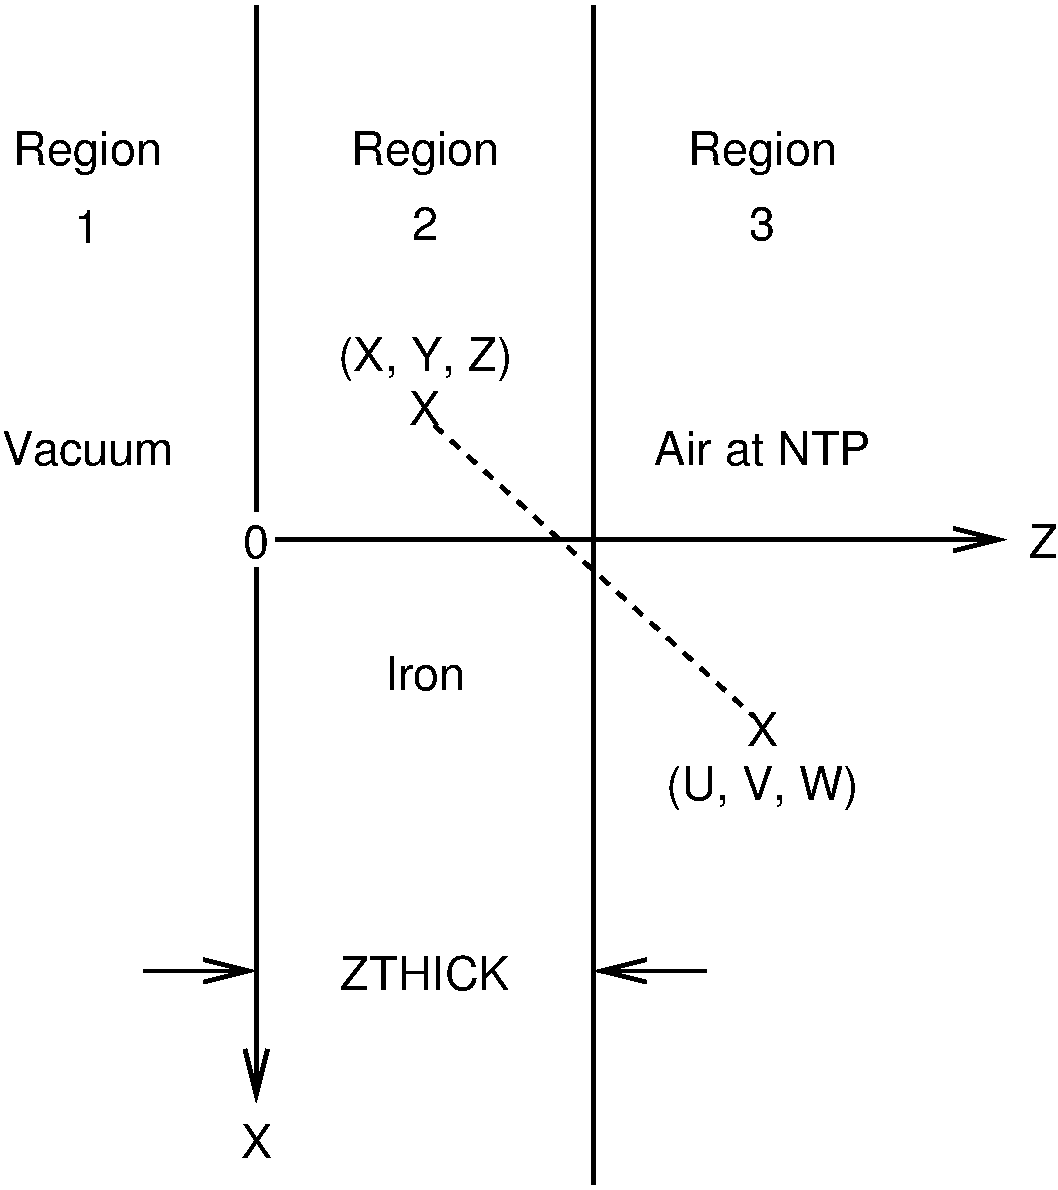
\includegraphics[width=10cm]{figures/3_region_ex}
   \end{center}
   \caption{A 3 region geometry example for HOWFAR.  The Y axis is into the
paper.}
   \label{fig_3_region_ex}
\end{figure}
Consider, as an example of how to write a {\tt HOWFAR} subroutine, the three
region geometry in fig~\ref{fig_3_region_ex}.  A particle is shown in
Region 2 with coordinates (X,Y,Z) and direction cosines (U,V,W).  We will
assume that the slab of thickness {\tt ZTHICK} is semi-infinite (x and
y-directions), and that particles are immediately discarded whenever they
go into Region 1 or Region 3.  The following {\tt HOWFAR} code is then
applicable:
\begin{verbatim}
     SUBROUTINE HOWFAR;
     COMIN/EPCONT,STACK/;      "common blocks needed in calculations"
     COMMON/GEOM/ZTHICK;       "slab thickness defined in main"
     IF(IR(NP) ~= 2) [IDISC=1; RETURN;]
     IF(W(NP) =  0.0) [RETURN; "particle going parallel to planes"]
     "check forward plane first since shower heading that way"
     "                                       most of the time"
     IF(W(NP) > 0.0) [DELTAZ=(ZTHICK-Z(NP))/W(NP); IRNEXT=3;]
     "otherwise, particle must be heading in backwards direction"
     ELSE [DELTAZ=-Z(NP)/W(NP); IRNEXT=1;]
     "now check with USTEP and reset things if necessary"
     IF(DELTAZ <= USTEP) [USTEP=DELTAZ; IRNEW=IRNEXT;]
     RETURN;  END;
\end{verbatim}
\index{HOWFAR!example}

\index{PLAN2P}
\index{\$PLAN2P}
A number of geometry subprograms and their macro equivalents are
distributed with the EGS Code System in order to make it easier to write
{\tt HOWFAR}.  For example, {\tt SUBROUTINE PLAN2P}, or its equivalent macro {\tt
\$PLAN2P}, could have been used in place of several lines above and the
program would have been easier to read.

\index{Bielajew, Alex}
For an advanced discussion of coding {\tt HOWFAR} routines, see Alex Bielajew's
PIRS-341 report ``HOWFAR and HOWNEAR: Geometry Modeling for Monte Carlo
Particle Transport''\cite{Bi95a}.


\subsection{Specifications for HOWNEAR}
\label{hownear}
\index{HOWNEAR!specifications}
\index{\$CALL-HOWNEAR}


As mentioned in section~\ref{hownear_macro}(page~\pageref{hownear_macro}),
for compatibility with previous  EGS4/PRESTA user codes,
EGSnrc formally requires a macro definition which defaults to:
\begin{verbatim}
REPLACE {$CALL-HOWNEAR(#);} WITH {CALL HOWNEAR({P1},X(NP),Y(NP),Z(NP),IRL);}
\end{verbatim}
where the variable {\tt \#} is {\tt tperp}, the closest distance to
any boundary.  If you are starting from scratch it is easiest to code
{\tt HOWNEAR} as a subroutine.
\index{EGS4}


{\tt SUBROUTINE HOWNEAR} is concerned with the geometry but its job is
somewhat simpler to define than for {\tt SUBROUTINE HOWFAR} since it need
only return one value, namely {\tt tperp}, the distance to the closest
boundary in {\bfseries any} direction.  Unlike {\tt HOWFAR}, {\tt HOWNEAR} passes the
transport parameters parameters to the subroutine as:
\begin{verbatim}
           SUBROUTINE HOWNEAR(tperp, x,y,z, irl);
\end{verbatim}
where \verb+x,y,z+ are the current positions of the particle and \verb+irl+
is its current region.  The rest of the information about the geometry is
passed in whatever {\tt COMMONs} contain the necessary information. In NRCC
user codes and the tutorial codes this is {\tt COMMON/GEOM/;} but it can be
called anything the user wants.

One simplification is that the routine does not have to handle regions
outside the geometry (as {\tt SUBROUTINE HOWFAR} must in order to have them
discarded).

In complex geometries, the mathematics of {\tt HOWNEAR} can become difficult and
sometimes almost impossible!  If it is easier for the user to compute
some lower bound to the nearest distance, this could be
used in {\tt HOWNEAR}.  In the worst case, one can return \verb+tperp+ as 0.0
in which case the code goes into single scattering mode if using the
exact boundary crossing algorithm.  In fact, this is an easy general way to
turn on single scattering throughout the entire geometry.

The following is an example of a {\tt HOWNEAR} routine for the geometry given
above in section~\ref{howfar} concerning {\tt HOWFAR}.
See also section~\ref{hownear_change} (page~\pageref{hownear_change}).
\begin{verbatim}
     SUBROUTINE HOWNEAR(tperp,X,Y.Z,IRL);
     COMMON/GEOM/ZTHICK; "slab thickness defined in main"
     tperp = min(Z,ZTHICK-Z);
     RETURN;  END;
\end{verbatim}
\index{HOWNEAR}



\subsection{Specifications for AUSGAB}
\label{ausgab}
\index{AUSGAB!specifications}

The subroutine {\tt AUSGAB} is called by EGS with the statement:
\begin{verbatim}
      CALL AUSGAB(IARG);
\end{verbatim}
The argument {\tt IARG} indicates the situation under which {\tt AUSGAB}
is being called.  {\tt IARG} can take on 35 values starting from zero
(i.e., {\tt IARG}=0 through {\tt IARG}=34), although only the first
five are called by default in EGSnrc.  The remaining 30 {\tt IARG}
values must be ``switched-on" by means of the array {\tt IAUSFL}.
The value for {\tt IARG} and the corresponding situations are given in
Table~\ref{tab_iausfl_low}.

On occasion one wants to terminate a particle histroy from withing AUSGAB.
To do this cleanly and efficiently set {\tt E(NP) = 0}. One can also set
the weight to zero if you do not want any {\tt EDEP} energy to be scored.

The {\tt IARG} values in table~\ref{tab_iausfl_low} are the ones
generally required in the majority of situations in which EGS is used
to simulate electromagnetic cascade shower development.  In particular,
{\tt IARG}=0 is useful whenever track lengths are being calculated or when
charged particle ionization loss is needed.  Also, as a check on energy
conservation, {\tt EDEP} can be summed in {\tt AUSGAB} for all {\tt IARG}
values less than 5.  The extended {\tt IARG} range allows the user to
extract additional information without making changes to the EGS coding.
To do this we have created the integer flag array, {\tt IAUSFL(J)},
for J=1 through 35.  It takes on values of 1 or 0 depending on whether
{\tt AUSGAB} is called or not, respectively.  For J=1 through 5, which
corresponds to {\tt IARG}=0 through 4, {\tt IAUSFL(J)=1} (default).
In other words, {\tt AUSGAB} is always called for the situations
listed in Table~\ref{tab_iausfl_low}.  For the remaining values of J,
corresponding to {\tt IARG}=5 through 34, {\tt IAUSFL(J)=0} (default).
The value for {\tt IARG} and the corresponding situations for this upper
set of {\tt IARG} values are shown in Table~\ref{tab_iausflg_other}.
\index{IAUSFL}
\index{IARG}
\index{PCUT}
\index{ECUT}
    \begin{table}[hbt]
\index{IAUSFL}
\index{IARG}
\index{PCUT}
\index{ECUT}
    \begin{center}
\caption{Values of {\tt IARG} which are on by default and for which energy is
deposited.}
    \label{tab_iausfl_low}
\vspace*{4mm}
    \begin{tabular}{ c   p{135mm}l  |}
    \hline
    {\tt IARG} & ~~~~~~~~~~~~~~~~~~~~~~~~~~~~~~~~Situation \\
    \hline
0	& Particle is going to be transported by distance TVSTEP.\\
    &\\
1	&Particle is going to be discarded because its energy is below the
cutoff {\tt ECUT} (for charged particles) or {\tt PCUT} (for photons)---but its energy
is larger than the corresponding PEGS cutoff AE or AP, respectively.\\
    &\\
2	& Particle is going to be discarded because its energy is below
both {\tt ECUT} and {\tt AE} (or {\tt PCUT} and {\tt AP}).\\
	&\\
3	& Particle is going to be discarded because the user requested it
(in {\tt HOWFAR} usually or by range rejection).  \\
	&\\
4	&The difference between the energy of the incident particle and
         all of the final products is being deposited locally. This
         energy is  due to sub-threshold relaxation events.\\
	&\\
\hline
\end{tabular}
\end{center}
\end{table}
\index{IARG} \index{IAUSFL}
\index{AUSGAB} \index{interogating EGSnrc}
    \begin{table}[htbp]
\index{Coster-Kronig electrons}
\index{IARG} \index{IAUSFL}
    \begin{center}
    \caption{Values of {\tt IARG} which are off by default.}
    \label{tab_iausflg_other}
     \vspace*{2mm}
    \begin{tabular}{ c c   p{125mm}l }
    \hline
    {\tt IARG} & {\tt IAUSFL} & ~~~~~~~~~~~~~~~~~~~~~~~~~~~~~~~~Situation \\
    \hline
5&6&  Particle has been transported by distance TVSTEP.\\
&&\\
6&7& A bremsstrahlung interaction is to occur and a call
             to BREMS is about to be made in ELECTR.\\
7&8& Returned to ELECTR after a call to BREMS was made.\\
&&\\
8&9& A Moller interaction is to occur and a call to
             MOLLER is about to be made in ELECTR.\\
9&10& Returned to ELECTR after a call to MOLLER was made.\\
&&\\
10&11&  A Bhabha interaction is to occur and a call to
             BHABHA is about to be made in ELECTR.\\
11&12& Returned to ELECTR after a call to BHABHA was made.\\
&&\\
12&13& An in-flight annihilation of the positron is to
             occur and a call to ANNIH is about to be made
             in ELECTR.\\
13&14& Returned to ELECTR after a call to ANNIH was made.\\
14&15&  A positron has annihilated at rest.\\
&&\\
15&16& A pair production interaction is to occur and a
             call to PAIR is about to be made in PHOTON.\\
16&17& Returned to PHOTON after a call to PAIR was made.\\
&&\\
17&18& A Compton interaction is to occur and a call to
             COMPT is about to be made in PHOTON.\\
18&19& Returned to PHOTON after a call to COMPT was made.\\
&&\\
19&20& A photoelectric interaction is to occur and a call
             to PHOTO is about to be made in PHOTON.\\
20&21& Returned to PHOTON after a call to PHOTO was made
             (assuming {\tt NP} is non-zero).\\
&&\\
21&22& Subroutine UPHI was just entered. Not entered in
all cases now since the sampling is done more efficiently directly in some
subroutines.\\
22&23& Subroutine UPHI was just exited.\\
&&\\
23&24& A coherent (Rayleigh) interaction is about to occur.\\
24&25& A coherent (Rayleigh) interaction has just occurred.\\
&&\\
25 &26& A fluorescent photon has just been created in RELAX.\\
26 & 27& A Coster-Kronig electron has just been created in RELAX.\\
27 &28& An Auger electron has just been created in RELAX.\\
&&\\
28 &29& A positron is about to annihilate at rest.\\
\hline
\end{tabular}
\end{center}
\end{table}

% Split the table onto the next page
\begin{table}[htbp]
    \begin{center}
    \caption{Values of {\tt IARG} which are off by default (continued).}
     \vspace*{2mm}
    \begin{tabular}{ c c   p{125mm}l }
    \hline
    {\tt IARG} & {\tt IAUSFL} & ~~~~~~~~~~~~~~~~~~~~~~~~~~~~~~~~Situation \\
    \hline
29 &30& A photonuclear event is about to occur and a call
            to PHOTONUC is about to be made in PHOTON.\\
30 &31& Returned to PHOTON after a call to PHOTONUC was made.\\
&&\\
31 &32& Electron impact ionization is about to occur and a call
            to eii\_sample is about to be made in MOLLER.\\
32 &33& Returned to MOLLER after a call to eii\_sample was made.\\
&&\\
33 &34& A fluorescent photon from relaxations was just discarded below
            PCUT and the energy stored in edep\_local.\\
34 &35& An electron from relaxations was just discarded below
            ECUT and the energy stored in edep\_local.\\
\hline
\end{tabular}
\end{center}
\end{table}

As an example of how to write an {\tt AUSGAB} subprogram, consider the previous
three region geometry (Fig. \ref{fig_3_region_ex}).  Suppose that we wish to
score (i.e., output on the line printer) only photons that go from Region 2
into Region 3.  The {\tt AUSGAB} subprogram that will accomplish this is given
below.  In this example we print out the stack variables plus {\tt IARG}.
\index{AUSGAB!example}
\begin{verbatim}
    SUBROUTINE AUSGAB(IARG);
    COMIN/STACK/;
    "only output information for photons that are discarded"
    "(by the user) in region 3"
    IF(IARG = 3 & IQ(NP) = 0 & IR(NP) =  3) [
        OUTPUT E(NP),X(NP),Y(NP),Z(NP),U(NP),V(NP),W(NP),
          IQ(NP),IR(NP),IARG;  (7G15.7,3I5);]
    RETURN;  END;
\end{verbatim}
The tutorial programs described in
section~\ref{tutorials}(page~\pageref{tutorials}) give examples of various
types of {\tt AUSGAB} routines.

\subsubsection{Checking for STACK overflow}
\index{EGS4} \index{\$MXSTACK}
\index{STACK overflow}
Unlike  EGS4, EGSnrc prevents the user from placing
too many particles on the {\tt STACK}. This is implemented via a macro
called {\tt \$CHECK-STACK(\#,\#);} which will terminate the execution if the
stack pointer exceeds {\tt \$MXSTACK}. This check takes some time (not much)
but to optimize the speed of a calculation, one might want to redefine it
as a null macro once one is moving to production runs.
\begin{verbatim}
      REPLACE {$CHECK-STACK(#,#);} WITH {;}
\end{verbatim}
Even if the above macro is nulled out, EGSnrc continues to verify that
there is adequate space on the stack whenever radiative splitting is being
used.
\index{\$CHECK-STACK}

\subsubsection{Status of the STACK at various AUSGAB calls}
\label{stack_status}
\index{STACK!order}
\index{EGS4}
In EGS4, the general rule was that after an interaction, the lowest energy
particle was always on the top of the {\tt STACK}. This general rule has
been relaxed in EGSnrc, partially because of the new physics, and partially
because memory is not as expensive as it once was.

\index{bound Compton scattering}
With the addition of relaxation events in EGSnrc, the possibilities
about what is on the stack after various events has become more complex
than in EGS4. For example, after a Compton scattering event in {\tt
EGS4}
({\tt IARG}=18), one could count on the {\tt STACK} having one more particle on it
compared to just before the call ({\tt IARG}=17). In EGSnrc, when bound compton
is being simulated, this is no longer the case.  Firstly, because of the
rejection techniques used to determine if the event actually took place
(see section~\ref{compton},page~\pageref{compton}) it is possible that only the
original photon is on the stack. At the opposite extreme, the scattered
photon and electron may be on the {\tt STACK} along with 2 or 3 relaxation
particles (fluorescent x-rays, Auger electrons, Coster-Kronig electrons).
Another complication occurs if Russian Roulette is being used since in this
case there can be events in which there is nothing left on the {\tt STACK} after
the event (e.g. after a pair event where the particles are discarded).
To help sort out these situations, EGSnrc has the variable {\tt
NPold} in {\tt COMIN STACK} which points to the position on the stack of the initiating particle
(the photon prior to Compton scattering, Rayleigh scattering, pair
production, photo-electric event or the electron prior to Moller scattering
or a bremsstrahlung event, etc).

Another change with EGSnrc is that the ordering of the resultant particles
is not rigorously set as lowest to highest energy.  This saves computing
time and with the reduced cost of memory, the issue of the size of the
{\tt STACK} is not so critical, at least not for low energy simulations ($<$100
MeV).  However, for high-energy simulations this may cause problems. To
overcome these the user code could define the macros {\tt
\$PARTICLE-SELECTION-MOLLER;} (where {\tt MOLLER} can be any interaction)
to sort the stack by energy after whatever interactions needed it. These
macros are by default null macros, but they are placed immediately after
the call to each subroutine which samples a type of event.
\index{\$PARTICLE-SELECTION-}

The ordering on the {\tt STACK} is summarized in the following.  Note that
the introduction of electron impact ionization and relaxation after other
than the photoelectric events has led to significant changes.
\begin{description}

\index{photoelectric interactions}
\item[Photoelectric] {\tt NPold} points at the photoelectron unless the initial
photon energy is $<$1~keV in which case there is an error message and an
electron with the photon's energy is created. Another exception occurs if
the photon's energy is less than the N-shell binding (which can only occur
for Z$\ge$96), in which case {\tt EDEP} is set to the photon's energy and a
photon of energy 0.0 is left at {\tt NPold}.  For normal events, the
particles from \verb^NPold+1^ to {\tt NP} are due to relaxation events.  If
internal Russian Roulette is being played (see section~\ref{rusrou}), it is
possible for {\tt NP} to be {\tt NPOLD - 1} after the event where there is
no fluorescent photon and all the resulting electrons are killed by the
Russian Roulette.  \index{Russian Roulette}

\index{bound Compton scattering}
\index{Compton scattering}
\item[Compton scattering] For Klein-Nishina modelling, the scattered photon and
electron are in {\tt NPold} and \verb^NPold+1 = NP^ respectively (i.e. the energy is not
ordered).  When bound compton scattering is
being modelled, there are several possibilities. At one extreme, since a
rejection technique is used, the scattering may not occur. In this case,
\verb^NPold = NP^.  If the scattering occurs, then the scattered photon and
compton electron are in \verb^NPold^ and \verb^NPold+1^, as in the Klein-Nishina case. If
there are any relaxation particles (i.e. \verb^NP > NPold+1^), they are found
in \verb^NPold+2^ to \verb^NP^.  There is a slight complication if the internal Russian
Roulette is being used (see section~\ref{rusrou})
since, if all the electrons disappear because of Russian Roulette, then
NPold=NP. To distinguish these two cases, the flag {\tt i\_survived\_RR}
can be used. It has a value 0 for the case of an unbound interaction being
rejected and has a value $>$ 0 if the interaction occurred and all
secondaries were eliminated by Russian Roulette.
\index{i\_survived\_RR}

\index{pair production}
\item[Pair Production] For pair production the electron and positron are
in {\tt NPold} and\\ \verb^NPold+1 = NP^ with the lower energy particle on the
top of the {\tt STACK} (at \verb^NP^). If internal Russian Roulette kills
the electron - positron pair, then,
\verb^NP = NPold-1^ unless this would leave \verb^NP = 0^, in which a
zero energy photon is placed on the {\tt STACK} with \verb^NP = 1^.

\index{Rayleigh scattering}
\item[Rayleigh scattering] In this case, the photon is still at
\verb^NPold^.

\index{bremsstrahlung!production}
\index{bremsstrahlung!splitting}
\item[Brem production] In this case, the resulting electron is
always at \verb^NPold^ and the photon is on top of the {\tt STACK} at \verb^NPold+1^, i.e. the
lowest energy particle is not necessarily on the top of the STACK. When
bremsstrahlung splitting is being used. The photons are between
\verb^NPold+1^ and
\verb^NP^. Note that they are not ordered by energy.

\index{Moller scattering}
\item[Moller scatter] There are 3 possible situations after a call to the
Moller routine. If a `standard' Moller scattering has occurred, the
resulting, lower energy electron is in \verb^NPold+1 = NP^ and the primary
is at \verb^NPold^. It is possible
that the incident electron's energy is below the threshold for creating a
secondary and the return is with \verb^NP^=\verb^NPold^. If this call to
Moller led to an electron impact ionization, the primary electron will be
at \verb^NPold^ and there may be relaxation events
from  \verb^NPold+1^ to \verb^NP^ although in the extreme case of all energy
deposition below threshold \verb^NP^=\verb^NPold^ and there is only the
primary electron.

\index{Bhabha scattering}
\item[Bhabha scatter] The resulting positron and electron are at
\verb^NPold^ and
\verb^NPold+1^, ordered by their energies.

\index{annihilation}
\item[Annihilation] The two resulting photons are at \verb^NPold^ and
\verb^NPold+1^
unless bremsstrahlung splitting is being used in which case the photons go
from \verb^NPold^ to \verb^N^P. The particle energies are not ordered.

\index{relaxation}
\item[Relaxation] There can be separate calls to AUSGAB after the
individual relaxation events (fluorescent photon, Coster-Kronig or Auger
electrons) but note that after the complete relaxation there may also be
ASUGAB calls post Moller, photoelectric and Compton and one should avoid
double counting.

\end{description}

\subsection{Terminating particle histories}
\label{termination}
\index{terminating particle history}
\index{weight}
\index{IDISC}
\index{WT=0.0}
The standard method to terminate a history is by setting
IDISC to a non-zero value in HOWFAR (see section~\ref{howfar},
page~\pageref{howfar}).  Another method is to set the weight of
a particle to 0.0, usually in AUSGAB under some conditions (e.g. when
doing Russian Roulette).  This technique is used in EGS4 by checking the
weight of a particle as it enters HOWFAR and setting IDISC non-zero if the
weight is zero.  This is somewhat wasteful since it means that various
parameters are calculated for this particle, despite the fact that it
is going to be discarded. In particular, we found that if we were also
using the standard photon forcing macro we got into an infinite loop.
This could have been corrected by re-coding the macro to handle weight
0.0 particles differently, but it was decided that we could save more
time by adding a test at the start of the new electron or new photon loops
whereby a particle is discarded immediately via the {\tt
USER-PHOTON-DISCARD} or {\tt USER-ELECTRON-DISCARD} if the weight is 0.0.
This generates a call to AUSGAB with {\tt IARG = 3}. Positrons discarded
this way do not create annihilation photons. Note that {\tt
ELKE} is not available with this call since it is assumed the particle
is being thrown away.  One should still have HOWFAR set {\tt IDISC = 1}
when the weight is 0.0, especially if the weight is set to zero for a
particle which is not new.


\subsection{Random number generators}
\label{rngs}
\index{random number generators}
\index{RANLUX}
\index{RANMAR}
\index{luxury level}

\index{EGS4}
EGSnrc is supplied with two random number generators, RANLUX
and RANMAR.  RANMAR is the generator used with EGS4 in the unix
distributions\cite{MZ91,Ma90a} and although it is known to fail certain
theoretical tests, we have no experience of it causing problems.
The RANLUX generator\cite{La94,Ja94}, which is treated as the default
generator with EGSnrc, is a similar sort of generator which comes
with a variety of ``luxury levels'', from 0 to 4 and a period of
greater than 10$^{165}$.  According to James, RANMAR has a
quality somewhere between luxury level 1 and 2 of RANLUX
and we have found
that it gives incorrect answers in some practical EGSnrc calculations
with luxury level 0. However, with luxury level 1 or higher we have
seen no problems.  We have utilized RANLUX as the default rng because
it allows explicit testing with higher quality sequences if there are
ever any doubts.

Both random number generators offer several important features. Firstly,
they are completely portable, producing the same sequences on different
machines, although RANMAR occasionally gets slightly out of sequence and
sometimes optimizers on a given machine will cause the sequences to differ.
We have not seen this behaviour with RANLUX.  An even more important
feature is that either generator can be initialized and guaranteed to
produce a random number sequence which is independent from other sequences.
This is very useful for doing runs in parallel on multiple machines.
\index{parallel processing}


The default generator is defined in {\tt
\$HEN\_HOUSE/specs/all\_common.spec} by the statement {\tt RANDOM =
\$(EGS\_SOURCEDIR)ranlux}. This can be changed to {\tt ranmar} or,
for individual user codes, it can be changed by adding the statement
{\tt RANDOM = \$(EGS\_SOURCEDIR)ranmar} to the {\tt user\_code.make}
file, somewhere before the {\tt SOURCES =} statement (if it exists).
See Report PIRS-877 for further information about {\tt make} files in
the EGSnrcMP environment\cite{Ka03}.

These files provide the following macros which the user is free to use in
their user code:
\begin{verbatim}
        ;COMIN/RANDOM/;
        $RANDOMSET#;
        $DEFAULT-LL   (1 by default)
        $RNG-INITIALISATION;    (which is only needed optionally)
        $INITIALIZE RNG USING # AND #; (a more useful version of the above)
        $STORE RNG STATE ON UNIT #;
        $PUT RNG STATE ON UNIT #;
        $RETRIEVE RNG STATE FROM UNIT #;
        $SHOW-RNG-STATE(#);
        $PRINT-RNG-STATE(#,#);
        $RNG-INPUTS(#,#,#,#);  (uses GET_INPUTS routine)
\end{verbatim}
\index{\$DEFAULT-LL}
To generate a random number, say {\tt RNUMBER}, include:
\begin{verbatim}
          $RANDOMSET RNUMBER;
\end{verbatim}
Wherever the user needs to use {\tt \$RANDOMSET\#;}, they must ensure
{\tt COMIN/RANDOM/} is present.
\index{RANDOM}
\index{macro!\$RANDOMSET}
\index{\$RANDOMSET}
If the user is happy with luxury level 1 and the same sequence for each
calculation, the RANLUX generator is self-initializing. However, to use
other luxury levels or other sequences, the user code should include
a statement of the type:
\begin{verbatim}
         $INITIALIZE RNG USING luxury_level AND iseed;
\end{verbatim}
where {\tt luxury\_level} is an integer between 0 and 4 and {\tt iseed}
is any positive integer (and if left 0, a default of {\tt 314159265} is used).
\index{\$INITIALIZE RNG USING}

For a standard production run of one of the NRC user codes (CAVRZnrc for
$^{60}$Co photons incident on a thimble chamber with splitting of 130) we
get the timing results shown in table~\ref{tab_ll_times}, although these
values are revised from the pre-2003 printings and depend on the details of
any simulation.  Given the iproblems encountered using luxury level 0,
luxury level 1 has been
adopted as the default with EGSnrc. However, given a new coding of RANMAR
to generate groups of random numbers using a function call, we find that
RANMAR is faster (by 5\% say overall).  The penalty ifor using higher
RANLUX luxury levels becomes increasingly more
important at higher luxury levels and a user may want to verify that for
their simulations, use of the higher level makes no difference. We would
appreciate being informed of any cases found where luxury level 1 was not
adequate.
\index{random number generators!timing}
\index{luxury level!timing}
\begin{table}[htb]
\begin{center}
\caption{Calculation times for runs with CAVRZnrc for the same calculations
along with estimates of the time taken by the random number generator at
different luxury levels.  The results for luxury level 0 are different when
high precision is obtained.\vspace{3mm}
\label{tab_ll_times}
}
\begin{tabular}{ |c c c c |}
\hline
Luxury level & total CPU time  & \multicolumn{2}{c|}{time taken by RANLUX} \\
             &  s &  s  & \%\\
\hline
&&&\\
0	&194	& 24 & 12\% \\
1	&210	& 39 & 18\% \\
2	&240	& 68 & 28\% \\
3	&315	& 142  &45\% \\
4	&415	& 242  &58\% \\
&&&\\
\hline
    \end{tabular}
    \end{center}
    \end{table}


When using the RANMAR generator, the initialisation looks like:
\begin{verbatim}
         $INITIALIZE RNG USING IXX AND JXX;
\end{verbatim}
where {\tt IXX} and {\tt JXX} are two integers seeds with:
\cen{{\tt  0$<$ IXX$<=$31328} and {\tt 0$<$JXX$<=$30081}}

The other macros are for use when saving the state of a random number
generator to disk and possibly restarting a run or other book keeping tasks.

There are two files available for use in codes doing correlated
sampling.  These files are:
\begin{verbatim}
       ranlux.correlations    or      ranmar.corrrelations
\end{verbatim}
These files define the macros:
\begin{verbatim}
        $STORE-RNG(#);
        $RESET-RNG(#);
\end{verbatim}
which store and reset an arbitrary number of random number states ($\le${\tt
\$MXRNGDIM} which is 5 by default).

Note: because of how the RANLUX generator is implemented, it is essential
that any redefined {\tt COMIN/RANDOM} must include an integer variable
called {\tt rng\_seed}. This variable is initialized to 999999 in {\tt
egs\_set\_default} which replaces {\tt BLOCK DATA} in the EGSnrcMP
environment\cite{Ka03}.
\index{RANDOM} \index{COMMON!RANDOM}
\index{random number generators}
\index{RANLUX}
\index{RANMAR}
\index{\$STORE-RNG}
\index{\$RESET-RNG}

\subsection{Summary of transport parameter}
\label{param_options}
\index{transport parameter summary}
\index{cross section options}


In many cases transport parameters and cross section options will be
controlled via an input file that uses a {\tt option = value} format
(\eg~all RZ user codes, all C++ codes). The following provides a summary
of the options available along with possible settings.

%%%%%%%%%%%%%%%%%%%%%%%%%%%%%%%%%%%%%%%%%%%%%%%%%%%%%%%%%%%%%%%%%%%%%%%%%%%%%%%
%
%  EGSnrc manual: transport parameters
%  Copyright (C) 2015 National Research Council Canada
%
%  This file is part of EGSnrc.
%
%  EGSnrc is free software: you can redistribute it and/or modify it under
%  the terms of the GNU Affero General Public License as published by the
%  Free Software Foundation, either version 3 of the License, or (at your
%  option) any later version.
%
%  EGSnrc is distributed in the hope that it will be useful, but WITHOUT ANY
%  WARRANTY; without even the implied warranty of MERCHANTABILITY or FITNESS
%  FOR A PARTICULAR PURPOSE.  See the GNU Affero General Public License for
%  more details.
%
%  You should have received a copy of the GNU Affero General Public License
%  along with EGSnrc. If not, see <http://www.gnu.org/licenses/>.
%
%%%%%%%%%%%%%%%%%%%%%%%%%%%%%%%%%%%%%%%%%%%%%%%%%%%%%%%%%%%%%%%%%%%%%%%%%%%%%%%
%
%  Author:          Frederic Tessier, 2011
%
%  Contributors:
%
%%%%%%%%%%%%%%%%%%%%%%%%%%%%%%%%%%%%%%%%%%%%%%%%%%%%%%%%%%%%%%%%%%%%%%%%%%%%%%%


\index{ECUT}
\begin{verbatim}
       Global ECUT=     Global (in all regions) electron transport cut
                        off energy (in MeV). If this input is missing,
                        AE(medium) will be used.
                        [ ECUT ]
\end{verbatim}
\index{PCUT}
\begin{verbatim}
       Global PCUT=     Global (in all regions) photon transport cut
                        off energy (in MeV). If this input is missing,
                        AP(medium) will be used.
                        [ PCUT ]
\end{verbatim}
\index{SMAX}
\begin{verbatim}
       Global SMAX=     Global (in all regions) maximum step-size
                        restriction for electron transport (in cm).
                        If missing, no geometrical step-size restrictions
                        will be employed. Note that if you use the default
                        EGSnrc electron-step algorithm, no SMAX-restriction
                        is necessary. Option is useful for transport in low
                        density materials (air) when PRESTA behaviour is
                        turned on (see below)
                        [ SMAXIR ]
\end{verbatim}
\index{ESTEPE}
\begin{verbatim}
       ESTEPE=          Maximum fractional energy loss per step.
                        Note that this is a global option only, no
                        region-by-region setting is possible. If missing,
                        the default is 0.25 (25%).
                        [ ESTEPE ]
\end{verbatim}
\index{XImax}
\begin{verbatim}
       XImax=           Maximum first elastic scattering moment per step.
                        Default is 0.5, NEVER use value greater than 1 as
                        this is beyond the range of MS data available.
                        [ XIMAX ]
\end{verbatim}
\index{boundary crossing algorithm}
\index{bca\_algorithm}
\index{exact\_bca}
\index{transport\_algorithm}
\begin{verbatim}
       Boundary crossing algorithm= EXACT (default), PRESTA-I
                        There are two selections possible: EXACT means
                        the algorithm will cross boundaries in a single
                        scattering (SS) mode, the distance from a boundary
                        at which the transition to SS mode is made is
                        determined by 'Skin depth for BCA' (see below).
                        The second option is PRESTA-I, if selected boundaries
                        will be crossed a la PRESTA, i.e. with lateral
                        correlations turned off and MS forced at boundaries.
                        Default is EXACT.
                        [ bca_algorithm, exact_bca ]
\end{verbatim}
\index{skin depth for BCA}\index{exact\_bca}
\index{skindepth\_for\_bca}
\begin{verbatim}
       Skin depth for BCA=
                        Determines the distance from a boundary (in elastic
                        MFP) at which the algorithm will go into single
                        scattering mode (if EXACT boundary crossing) or
                        switch off lateral correlations (if PRESTA-I boundary
                        crossing). Default value is 3 for EXACT or
                        exp(BLCMIN)/BLCMIN for PRESTA-I (see the PRESTA paper
                        for a definition of BLCMIN). Note that if you choose
                        EXACT boundary crossing and set Skin depth for BCA
                        to a very large number (e.g. 1e10), the entire
                        calculation will be in single-scattering mode. If you
                        choose PRESTA-I boundary crossing and make Skin depth
                        for BCA large, you will get default EGS4 behaviour
                        (no PRESTA).
                        [ skindepth_for_bca ]
\end{verbatim}
\index{electron step algorithm}
\begin{verbatim}
       Electron-step algorithm= PRESTA-II (default), PRESTA-I (legacy)
                        Determines the algorithm used to take into account
                        lateral and longitudinal correlations in a
                        condensed history step.
                        [ transport_algorithm ]
\end{verbatim}
\index{spin effects}
\index{spin\_effects}
\begin{verbatim}
       Spin effects=    Off, On (default)
                        Turns off/on spin effects for electron elastic
                        scattering. Spin On is ABSOLUTELY necessary for
                        good backscattering calculations. Will make a
                        difference even in `well conditioned' situations
                        (e.g. depth dose curves for RTP energy range
                        electrons).
                        [ spin_effects ]
\end{verbatim}
\index{brems angular sampling}
\index{IBRDST}
\begin{verbatim}
       Brems angular sampling= Simple, KM (default)
                        If Simple, use only the leading term of the Koch-Motz
                        distribution to determine the emission angle of
                        bremsstrahlung photons. If KM, complete
                        modified Koch-Motz 2BS is used (modifications
                        concern proper handling of kinematics at low energies,
                        makes 2BS almost the same as 2BN at low energies).
                        [ IBRDST ]
\end{verbatim}
\index{brems cross section}
\index{ibr\_nist}
\begin{verbatim}
       Brems cross sections= BH (default), NIST, NRC
                        If BH is selected, the Bethe-Heitler bremsstrahlung
                        cross sections (Coulomb corrected above 50 MeV)
                        will be used. If NIST is selected, the NIST brems
                        cross section data base (which is the basis for
                        the ICRU radiative stopping powers) will be employed.
                        Differences are negligible for E > ,say, 10 MeV,
                        but significant in the keV energy range. If NRC is
                        selected, the NRC brems cross-section data base will
                        be used, which is a version of the NIST data base
                        with corrected electron-electron brems contributions
                        (corrections to the NIST data is typically only
                        significant for low values of the atomic number Z
                        and for k/T < 0.005).
                        [ ibr_nist ]
\end{verbatim}
\index{triplet production}
\index{itriplet}
\begin{verbatim}
       Triplet production= On or Off (default).  Turns on/off simulation
                        of triplet production.  If On, then Borsellino's
                        first Born approximation is used to sample triplet
                        events based on the triplet cross-section data.
                        [ itriplet ]
\end{verbatim}
\index{bound Compton scattering}
\index{IBCMP}
\begin{verbatim}
       Bound Compton scattering=  On, Off, Simple or norej (default)
                        If Off, Compton scattering will be treated with
                        Klein-Nishina, with On Compton scattering is
                        treated in the Impulse approximation.
                        With Simple, the impulse approximation incoherent
                        scattering function will be used (i.e., no Doppler
                        broadenning). With norej the actual total bound
                        Compton cross section is used and there are no
                        rejections at run time.
                        Make sure to turn on for low energy applications,
                        not necessary above, say, 1 MeV.
                        [ IBCMP ]
\end{verbatim}
\index{radiative Compton corrections}
\index{radc\_flag}
\begin{verbatim}
       Radiative Compton corrections= On or Off (default). If On, then
                        include radiative corrections for Compton scattering.
                        Equations are based on original Brown & Feynman
                        equations (Phys. Rev. 85, p 231--1952).  Requires
                        a change to the user codes Makefile to include
                        $(EGS_SOURCEDIR)rad_compton1.mortran in the
                        SOURCES (just before
                        $(EGS_SOURCEDIR)get_inputs.mortran).
                        [ radc_flag ]
\end{verbatim}
\index{electron impact ionization}
\index{eii\_flag}
\begin{verbatim}
       Electron Impact Ionization= Off (default), On, casnati, kolbenstvedt,
                        gryzinski or penelope.  If set to On or ik, then
                        use Kawrakow's theory to derive EII cross-sections.
                        If set to casnati, then use the cross-sections of
                        Casnati (from file $HEN_HOUSE/data/eii_casnati.data).
                        Similar for kolbenstvedt, gryzinski and penelope.
                        This is only of interest in kV X-ray calculations.
                        Note that the user can supply their own EII
                        cross-section data as well. The requirement is that
                        the file eii_suffix.data exists in the $HEN_HOUSE/data
                        directory, where suffix is the name specified.
                        Entry is case-sensitive except for Off, On or ik.
                        [ eii_flag, eii_xfile ]
\end{verbatim}
\index{pair angular sampling}
\index{IPRDST}
\begin{verbatim}
       Pair angular sampling= Off, Simple (default), KM.
                        If off, pairs are set in motion at an angle m/E
                        relative to the photon direction (m is electron rest
                        energy, E the photon energy). Simple turns on
                        the leading term of the angular distribution
                        (this is sufficient for most applications),
                        KM (comes from Koch and Motz) turns on using 2BS
                        from the article by Koch and Motz.
                        Default is Simple, make sure you always use
                        Simple or KM
                        [ IPRDST ]
\end{verbatim}
\index{pair cross sections}
\index{pair\_nrc}
\begin{verbatim}
       Pair cross sections= BH (default) or NRC.  If set to BH, then use
                        Bethe-Heitler pair production cross-sections.  If set
                        to NRC, then use NRC pair production cross-sections
                        (in file $HEN_HOUSE/data/pair_nrc1.data).  Only
                        of interest at low energies, where the NRC cross-
                        sections take into account the asymmetry in the
                        positron-electron energy distribution.
                        [ pair_nrc ]
\end{verbatim}
\index{photon cross sections}
\index{photon\_xsections}
\begin{verbatim}
       Photon cross sections= Photon cross-section data.  Current options are
                        si (Storm-Israel--the default), epdl (Evaluated Photon
                        Data Library), and xcom.  Allows the user to use photon
                        cross-sections other than the default PEGS4 (Storm-
                        Israel) values.  Note that the user can supply their
                        own cross-section data as well.  The requirement is
                        that the files
                        photon_xsections_photo.data,
                        photon_xsections_pair.data,
                        photon_xsections_triplet.data, and
                        photon_xsections_rayleigh.data exist in the
                        $HEN_HOUSE/data directory, where photon_xsections
                        is the name specified.
                        Entry is case-sensitive except for the pegs4 option.
                        [ photon_xsections ]
\end{verbatim}
\index{photon cross sections!output}
\index{xsec\_out}
\begin{verbatim}
       Photon cross-sections output= Off (default) or On.  If On, then
                        a file $EGS_HOME/user_code/inputfile.xsections is
                        output containing photon cross-section data used.
                        [ xsec_out ]
\end{verbatim}
\index{compton cross sections}
\index{comp\_xsections}
\begin{verbatim}
       Compton cross sections= Bound Compton cross-section data.  User-
                        supplied bound Compton cross-sections in the file
                        $HEN_HOUSE/data/comp_xsections_compton.data, where
                        comp_xsections is the name supplied for this input.
                        This is only used if Bound Compton scattering= Simple
                        and is not available on a region-by-region basis
                        (see below).  The default file (ie in the absence
                        of any user-supplied data) is compton_sigma.data.
                        [ comp_xsections ]
\end{verbatim}
\index{Rayleigh scattering}
\index{Rayleigh scattering!custom form factors}
\index{IRAYLR}
\begin{verbatim}
       Rayleigh scattering= Off, On (default), custom
                        If On, turns on coherent (Rayleigh) scattering.
                        Default is On. Should be turned on for low energy
                        applications. If custom, user must provide media names
                        and form factor files for each desired medium. The
                        rest of the media use the default atomic form factors.
                        Not set to On by default for historical reasons since
                        a PEGS4 data set is not required anymore.
                        [ IRAYLR ]
\end{verbatim}
\index{iray\_ff\_media}
\begin{verbatim}
       ff media names = A list of media names (must match media found in
                        PEGS4 data file) for which the user is going to
                        provide custom Rayleigh form factor data.
                        [ iray_ff_media($MXMED) ]
\end{verbatim}
\index{iray\_ff\_file}
\begin{verbatim}
       ff file names = A list of names of files containing the Rayleigh
                       form factor data for the media specified by
                       the ff media names = input above.  Full directory
                       paths must be given for all files, and for each medium
                       specified, iray_ff_media(i), there must be a
                       corresponding file name, iray_ff_file(i).  For
                       example files, see the directory
                       $HEN_HOUSE/data/molecular_form_factors.
                       [ iray_ff_file($MXMED) ]
\end{verbatim}
\index{photonuclear attenuation}
\index{IPHOTONUCR}
\begin{verbatim}
       Photonuclear attenuation= Off (default) or On
                        If On, models the photonuclear effect. Current
                        implementation is crude. Available on a
                        region-by-region basis (see below)
                        [ IPHOTONUCR ]
\end{verbatim}
\index{photonuclear cross sections}
\index{photonuc\_xsections}
\begin{verbatim}
       Photonuclear cross sections= Total photonuclear cross sections. User-
                        supplied total photonuclear cross-sections in
                        $HEN_HOUSE/data/photonuc_xsections_photonuc.data,
                        where photonuc_xsections is the name supplied for
                        this input (case sensitive). In the absence of
                        any user-supplied data, or if photonuc_xsections
                        is set to 'default', the default file is
                        iaea_photonuc.data.
                        [ photonuc_xsections ]
\end{verbatim}
\index{photoelectron angular sampling}
\index{IPHTER}
\begin{verbatim}
       Photoelectron angular sampling= Off or On (default)
                        If Off, photo-electrons get the direction of the
                        `mother' photon, with On, Sauter's formula is
                        used (which is, strictly speaking, valid only for
                        K-shell photo-absorption).
                        If the user has a better approach, replace the macro
                            $SELECT-PHOTOELECTRON-DIRECTION;
                        The only application encountered where this option
                        made a small difference was a big ion chamber
                        (cavity size comparable with electron range)
                        with high-Z walls in a low energy photon beam.
                        [ IPHTER ]
\end{verbatim}
\index{atomic relaxations}
\index{IEDGFL}
\begin{verbatim}
       Atomic relaxations= Off, On, eadl (default), simple
                        On defaults to eadl.
                        When simulating atomic relaxations:
                        - In photo-electric absorption events, the element
                          (if material is mixture) and the shell the photon
                          is interacting with are sampled from the appropriate
                          cross sections
                        - Shell vacancies created in photoelectric,
                          compton and electron impact ionization events
                          are relaxed via emission of fluorescent X-Rays,
                          Auger and Koster-Cronig electrons.
                          The eadl option features a more accurate treatment
                          of relaxation events and uses binding energies
                          consistent with those in of the photon cross sections
                          used in the simulation.  If using mcdf-xcom or
                          mcdf-epdl photon cross sections, you cannot use
                          the simple option and this will automatically get
                          reset to eadl. Make sure to use eadl or simple for
                          low energy applications.
                          [ IEDGFL ]
\end{verbatim}

\noindent
Atomic relaxations, Rayleigh scattering, Photoelectron angular sampling,
Bound Compton scattering and photonuclear effect
can also be turned On/Off on a region-by-region basis. An example for
Atomic relaxations on a region-by-region basis is:

\begin{verbatim}
       Atomic relaxations= On in Regions   or
       Atomic relaxations= Off in regions
\end{verbatim}

Then define the regions in which you want
the feature to be turned on:

\begin{verbatim}
       Bound Compton start region=
       Bound Compton stop region=
                or
       Rayleigh start region=
       Rayleigh stop region=
                or
       Relaxations start region=
       Relaxations stop region=
                or
       PE sampling start region=
       PE sampling stop region=
\end{verbatim}
each followed by a list of one or more
start and stop regions separated by commas.
Example:
\begin{verbatim}
        Atomic relaxations= On in Regions
        Relaxations start region=  1, 40
        Relaxations stop region=  10, 99
\end{verbatim}
will first turn off relaxations everywhere and
then turn on in regions 1-10 and 40-99.
Note that the input is checked against minimum
and maximum region numbers and ignored if
\verb+start region < 1+ or \verb+stop_region > $MXREG+ or
\verb+start region > stop region+.

\verb+ECUT+, \verb+PCUT+ and \verb+SMAX+ can also be set on a
region-by-region basis. To do so, include in the input file
\begin{verbatim}
         Set XXXX=              f_value1, f_value2, ...
         Set XXXX start region= i_value1, i_value2, ...
         Set XXXX stop region=  j_value1, j_value2, ...
\end{verbatim}
where \verb+XXXX+ is \verb+ECUT+, \verb+PCUT+ or \verb+SMAX+,
\verb+f_value1+, \verb+f_value2+,...
are the desired values for \verb+XXXX+ and \verb+i_value_i+ and
\verb+j_value_i+ are the start and stop regions.


\subsection{Variance Reduction Options}
\label{VRO}
\index{variance reduction}
Three forms of variance reduction techniques have been implemented directly
into the EGSnrc system in order to allow for more efficient calculations.
With EGS4 user codes they had to be implemented via calls to {\tt
AUSGAB} or
other means, and this led to inefficiencies.  In all three cases, if the
user does nothing to turn on these options explicitly, then they are NOT
used.
\index{EGS4}

\subsubsection{Range rejection}
\label{range_rejection}

\index{range rejection}
\index{variance reduction}
\index{variance reduction!range rejection}
\index{E\_RANGE}
Within EGSnrc the range of the electron is available at every step. This is
not the true range, but the range determined by:
\[ {\tt E\_RANGE} = \int_{E_{min}}^E \frac{dE^\prime}{L(E^\prime,AE)}\]
where $L(E^\prime,AE)$ is the restricted stopping power for a given value
of AE and $E_{min}$ is the lowest energy for which PEGS4 produces a
stopping power (this is somewhat less than AE, but not much).
The value of {\tt E\_RANGE} is an
upper limit on the distance an electron can travel in the simulation
because discrete events may shorten the pathlength.

\index{\$RANGE-DISCARD}
\index{macro!\$RANGE-DISCARD}
Range rejection is implemented by a macro {\tt \$RANGE-DISCARD} checks
the electron range against the distance to the nearest boundary on
every step. The history is terminated whenever the range is shorter than
the distance to the boundary and if requested by the user.  Since the
range and distance are calculated for other purposes, this check is
very fast and can save a large amount of time, especially in large
regions. Since this is a user controlled discard, it goes via the {\tt
USER-ELECTRON-DISCARD}, generating and {\tt {\tt IARG} = 3}   call to {\tt
AUSGAB}.
\index{USER-ELECTRON-DISCARD}   \index{AUSGAB}

This technique
does involve an approximation since the electron could emit a
brem photon which could escape the region, even if the electron
itself could not.  To control the extent of this approximation, the range
rejection is done only if the electron's energy is below an energy
threshold which can be set for every region, viz {\tt e\_max\_rr}. By
judicial choice of this value, the approximation can be made very accurate
while still obtaining very significant gains in efficiency (see
ref~\cite{Ro95} for a detailed discussion, where the parameter {\tt ESAVE}
in that paper is equivalent to {\tt e\_max\_rr} here).

Range rejection is implemented on a regional basis by setting the flags
{\tt i\_do\_rr(irl)} to 1 for all regions {\tt irl} for which range
rejection is required and by assigning values to the array {\tt
e\_max\_rr(irl)}. Note that if {\tt e\_max\_rr(irl)} is not assigned a value,
its default value of 0.0 effectively turns off range rejection, even
if {\tt i\_do\_rr(irl)} value is 1.  Both arrays are in {\tt
COMIN/EGS-VARIANCE-REDUCTION}. They need be set before the first
call to {\tt SHOWER}.  Note that {\tt e\_max\_rr(irl)} refers to the
electrons total energy (i.e. includes the rest mass, as does {\tt ECUT}).
\index{EGS-VARIANCE-REDUCTION} \index{e\_max\_rr}
\index{i\_do\_rr} \index{range rejection}

The user is also free to implement other, possibly more efficient forms of
range rejection. This is done by defining the macro {\tt
\$USER-RANGE-DISCARD} which is called immediately after the above macro
since in general, the macro {\tt \$RANGE-DISCARD} executes very quickly
and can avoid use of the user's, presumably more time consuming range
rejection.  An example of {\tt
\$USER-RANGE-DISCARD} is given in CAVRZnrc where range rejection is done on
any particle which cannot reach the region where the dose is required. This
can terminate many histories earlier than {\tt \$RANGE-DISCARD} because it
tests against getting to the region of interest as opposed to just getting
out of the local region.  However, it requires some approximations and
takes longer to compute on each step.
\index{\$USER-RANGE-DISCARD}
\index{range rejection}

\subsubsection{Bremsstrahlung Splitting}
\label{brem_splitting}
\index{bremsstrahlung!splitting}
\index{variance reduction!brem splitting}
\index{nbr\_split}
Bremsstrahlung splitting is a technique which can provide a factor of 4 or
more
improvement in efficiency when modelling brem beams generated
by medical accelerators\cite{Ro95}.  Each time an electron emits a photon,
the simulation emits an arbitrary number of brem photons with
their weight suitably reduced. The electron's energy is decremented by the
energy given off by one of these photons. This preserves accurate
energy loss straggling of the electron at the expense of no longer having
exact energy conservation for each history, although energy is conserved
``on average''.  The advantage of doing this splitting within the routine
BREMS is that various constants for the electron's energy are only
calculated once and the sampling is therefore faster.  The electron is
always found at \verb^NPold^ on the {\tt STACK} and the photons are not sorted by energy.

To accomplish bremsstrahlung  splitting, the variable {\tt nbr\_split} which
is in\\ {\tt COMIN/EGS-VARIANCE-REDUCTION} must be set to the number of
brem photons wanted at each discrete interaction. See
section~\ref{rad_split} (page~\pageref{rad_split}).

There are no internal limits on the number of splits that may be used
except that the stack size, {\tt \$MXSTACK}, may not be exceeded.  The user
code can override the value of {\tt \$MXSTACK} if a larger value is needed.

\index{Russian Roulette}
Note that once
set, EGSnrc will split brem at all generations.  This is
appropriate when Russian Roulette is being played since it means that
second generation bremsstrahlung photons will have the same weight as first
generation photons.  However, it can become very time consuming and counter
productive when Russian Roulette is not being played because second and
higher order bremsstrahlung photons have much smaller weights. To overcome
this problem, the user might want to use calls to {\tt AUSGAB} to reduce the
value of {\tt nbr\_split} after each first generation bremsstrahlung
interaction and then re-initialize it at the start of the next history.
This is the technique used in the BEAM code\cite{Ro95,Ro98a}.
\index{BEAM code}


\subsubsection{Russian Roulette}
\label{rusrou}
\index{variance reduction!Russian Roulette}
\index{Russian Roulette}
\index{i\_play\_RR}
\index{prob\_RR}
\index{nbr\_split}
\index{i\_survived\_RR}
\index{EGS4}
Russian Roulette is a standard variance reduction technique which in {\tt
EGS4}
had to be done via call to {\tt AUSGAB}. This works but is somewhat slower than
need be. For example, say that the particles created in a pair
event are to be discarded. In EGS4 the sampling routines must still
determine all their parameters and then remove them from the {\tt STACK} whereas
in EGSnrc Russian Roulette is played prior to the sampling, and then
not done if not needed. In less dramatic cases, the EGSnrc approach avoids
extra steps were the EGS4 system had to go through to eliminate the
particle.

Russian Roulette, as implemented in EGSnrc, is a user option which is turned on by
setting the integer flag {\tt i\_play\_RR} to 1 and by setting the
probability {\tt prob\_RR} to an appropriate value. Both these parameters
are in {\tt COMIN/EGS-VARIANCE-REDUCTION}.

If Russian Roulette is being used in conjunction with bremsstrahlung
splitting, the appropriate value of {\tt prob\_RR} is {\tt 1./nbr\_split}.

The integer variable {\tt i\_survived\_RR} is also in  {\tt
COMIN/EGS-VARIANCE-REDUCTION}. It is 0 if Russian Roulette is not played or
if all particles survived when Russian Roulette was played on the previous
interaction.  Otherwise, its value tells how many particles were discarded
by Russian Roulette on the previous interaction.
\index{Russian Roulette}



\subsection{Complete Users Codes Examples}
For several examples of complete EGSnrc user codes, see the TUTOR codes
discussed in section~\ref{tutorials}. The EGSnrc distribution also comes
with several NRC user codes which have examples of many features\cite{Ro00}
but they have grown up over the years and have been patched so often that
they are hard to follow.

\subsection{Some Utility codes}
\subsubsection{SUBROUTINE WATCH}
\index{WATCH}
\index{IWATCH}
\index{SUBROUTINE WATCH}
\index{EGS\_Windows}
{\tt SUBROUTINE WATCH} is in the file {\tt nrcaux.mortran}. With a few simple
statements in a user code, it can print a listing to the screen of what is
happening in each history.  This is very useful for debugging purposes. We
strongly recommend that it be used with all user codes.  It also creates
output suitable for the EGS\_Windows graphic display system\cite{TR99a}.
For more information, see {\tt tutor4.mortran} for an example of a simple
code with WATCH included (see section~\ref{tutor4}, page~\pageref{tutor4}).

\subsubsection{ranlux\_test.mortran and ranmar\_test.mortran}
\index{test!RANLUX}
\index{test!RANMAR}
\index{ranlux\_test.mortran}
\index{ranmar\_test.mortran}
\index{random number generators!portability}
These little codes can be used to verify that the ranlux and
ranmar random number generators are working correctly on your
system. Since these generators produce machine independent
random numbers, the values should be identical on all machines.
They are found on {\tt \$HEN\_HOUSE/user\_codes/ranlux\_test/} and  {\tt
\$HEN\_HOUSE/user\_codes/ranmar\_test/}. Each can be compiled and executed
as a user code.  The output is self explanatory but basically
they both calculate
1 million random numbers and compare their sums to the expected values.
See the comments at the top of the source code for further information.

Note that even with identical random number sequences, the results of a
full EGSnrc calculation may not be identical on different machines or at
different optimization levels.  This is because statements like
\begin{verbatim}
          IF ( A < C/D) ) GOTO n;
\end{verbatim}
may branch differently, depending on how many digits are stored in C/D on
different machines or at different levels of optimization.

\subsubsection{EXAMIN}
\index{EXAMIN}
\index{user codes!EXAMIN}
\label{examin}
\index{xmgr}
\index{HOW\_to\_get\_xmgr}
The user code EXAMIN is distributed with the system. It provides easy
access to the underlying data produced by PEGS4. EXAMIN tabulates many
cross sections and if you have installed the
{\tt xmgr} graphics package it also plots the data (see the file\\ {\tt
\$HEN\_HOUSE/utils/HOW\_to\_get\_xmgrace} for information about {\tt
xmgrace}).
The code outputs quantities such as the gamma mean free path, the relative
contributions from the various components of the photon cross sections, the
mean free path to discrete interactions for electrons, etc.  It is a useful
template for seeing how to access the data base.  Note that the data
presented are those from PEGS4. Although EGSnrc can model bound Compton
scattering, this is done using a rejection technique and this code does not
allow access to the bound Compton cross sections, only the Klein Nishina
cross sections.
%  If you are using the {\tt xmgrace} package instead of the
%  {\tt xmgr} package, {\tt xmgr} must be replaced by {\tt xmgrace}
%  in the source code for {\tt examin.mortran} in two obvious places.

% \subsubsection{show\_settings}
% \label{settings}
% \index{show\_settings}
% \index{settings}
% This is a simple script which will display all the variables and aliases
% which are set or defined for use with the EGSnrc system (mostly in {\tt
% Cshrc\_additions\_for\_egsnrc}).


% \subsubsection{test\_distribution}
% \label{test_distribution}
% \index{test\_distribution}
% \index{test!distribution}
%
% This script is found on {\tt \$HEN\_HOUSE/scripts} after installation
% and the command {\tt test\_distribution} is aliased to it in {\tt
% egsnrc\_cshrc\_additions} and {\tt egsnrc\_bashrc\_additions}.
% It is executed with no arguemnts, and to capture the output as:
% \begin{verbatim}
             % test_distribution >& test_distribution.output &
% \end{verbatim}
% This script compiles all the user and tutorial codes and runs them with
% short
% test input files.  You must read the output file carefully since it will
% continue even when some or all of the codes fail to compile or execute!
% Once you get this script to execute cleanly
% your system is definitely in good shape. The results
% for running this script on various systems are found on {\tt
% \$HEN\_HOUSE/test\_distribution\_outputs}.
% \index{test\_distribution\_outputs}

\subsection{Latest additions}
\subsubsection{Charged particle transport under electromagnetic fields}
\label{EMF_macros_implementation}
Bielajew's EGS4 macros for transport under electromagnetic (EM) fields were adapted for EGSnrc by Amir Keyvanloo and
others from the Cross Cancer Institute in Edmonton. These macros have been included in the current EGSnrc release.
To turn on transport under EM fields, users must add the file {\tt emf\_macros.mortran} to the {\tt MORTRAN} sources to be compiled. The subroutine {\tt ELECTR} in {\tt egsnrc.mortran} contains macro replacements which are empty by default, but which are activated when including the EM macros.

To include these macros in a MORTRAN user code, append {\tt emf\_macros.mortran} to {\tt SOURCES} variable in file
{\tt user\_code.make} (user\_code can be any MORTRAN user code other than a BEAMnrc user code):
\begin{verbatim}
 ...
SOURCES = \
        $(EGS_SOURCEDIR)egsnrc.macros \
        ...
        $(EGS_SOURCEDIR)emf_macros.mortran \
        $(USER_CODE).mortran \
        ...
        $(EGS_SOURCEDIR)get_inputs.mortran\
        $(EGS_SOURCEDIR)get_media_inputs.mortran\
        ...
        $(EGS_SOURCEDIR)pegs4_routines.mortran \
        $(EGS_SOURCEDIR)egsnrc.mortran
 ...
\end{verbatim}

To include these macros in an existing BEAMnrc user code, append {\tt emf\_macros.mortran} to {\tt SOURCES} variable in file
{\tt source.make}:
\begin{verbatim}
SOURCES = $(EGS_SOURCEDIR)egsnrc.macros \
          ...
          $(EGS_SOURCEDIR)emf_macros.mortran \
          ...
          $(BEAM_HOME)beamnrc_user_macros.mortran \
          ...
          $(BEAM_CODE)_macros.mortran \
          $(EGS_SOURCEDIR)egs_utilities.mortran \
          $(BEAM_HOME)beam_main.mortran\
          $(BEAM_HOME)beamnrc.mortran \
          ...
          $(EGS_SOURCEDIR)egsnrc.mortran

\end{verbatim}
In the case of a BEAMnrc source library, append {\tt emf\_macros.mortran} to {\tt LIB\_SOURCES} variable in file
{\tt source.make}:
\begin{verbatim}
LIB_SOURCES = $(BEAM_HOME)beam_lib.macros \
          $(EGS_SOURCEDIR)egsnrc.macros \
          ...
          $(EGS_SOURCEDIR)emf_macros.mortran \
          ...
          $(BEAM_HOME)beamnrc_user_macros.mortran \
          ...
          $(BEAM_CODE)_macros.mortran \
          $(BEAM_HOME)beam_lib.mortran\
          $(BEAM_HOME)beamnrc.mortran \
          ...
          $(EGS_SOURCEDIR)egsnrc.mortran
\end{verbatim}

For C++ user codes one must append {\tt emf\_macros.mortran} to the {\tt EGSPP\_USER\_MACROS} variable in
the {\tt Makefile}:
\begin{verbatim}
 ...
# Specify the name of the user code.
# The name of the executable is determined from this variable.
#
USER_CODE = cavity

# The following can be used to add user macros and mortran subroutines.
# The file(s) specified here are added after egsnrc.macros, machine.macros
# and egs_c_interface2.macros but before any files that have
# executable code.
#
#EGSPP_USER_MACROS = cavity.macros
EGSPP_USER_MACROS = cavity.macros  \
                    $(EGS_SOURCEDIR)emf_macros.mortran
 ...
\end{verbatim}

Details of the field and the step size restriction are entered by input in the MC transport parameters section:
\begin{itemize}
\item For magnetic fields:
\begin{verbatim}
:start MC transport parameter:
 ...
 Magnetic Field = 0, 1.5, 0 # magnetic field in T
 EM ESTEPE = 0.02
 ...
:stop MC transport parameter:
\end{verbatim}

\item For electric fields:
\begin{verbatim}
:start MC transport parameter:
 ...
 Electric Field = 0, 3, 0 # electric field in V/cm
 EM ESTEPE = 0.02
 ...
:stop MC transport parameter:
\end{verbatim}
\end{itemize}

Please note than one can define both, an electric and a magnetic field. The {\tt EM ESTEPE}
entry sets the value for the step size restrictions based on energy loss, field change and
direction change. For instance, in the static $\vec{B}_0$ field case of section \ref{EMF_macros_algorithm},
{\tt EM ESTEPE} corresponds to the $\delta$ value of Eq(\ref{uchange_restriction}). By default it is set to 0.02.

\subsubsection{EADL atomic relaxations}
In EGSnrc the relaxation cascade of inner shell vacancies is an independent process that is initiated each time
a vacancy is created
\begin{itemize}
  \item In photo-absorption, bound Compton scattering, and electron impact ionization processes.
  \item Future: triplet production, electron-electron bremsstrahlung
\end{itemize}

The default implementation include relaxation events from:
\begin{itemize}
\item All shells with binding energies above 1 keV
\item All radiative and non-radiative transitions to/from K-, LI-, LII and LIII-shells
\item All radiative and non-radiative transitions to/from ``average'' M and N-shells.
\end{itemize}

An option to remove above limitations by using EADL atomic relaxation data has been available in EGSnrc since 2011.
% User must set macro \$EADL\_RELAX to .true. in file egsnrc.macros.
The way to turn on EADL relaxation is by setting macro \$EADL\_RELAX to .true. in egsnrc.macros or in the user-code. It is currently set to .false. by default.

%following may be needed to get next section start on odd page
%\newpage
%\mbox{}


%%%%%%%%%%%%%%%%%%%%%%%%%%%%%%%%%%%%%%%%%%%%%%%%%%%%%%%%%%%%%%%%%%%%%%%%

%		Tutorial Programs

%%%%%%%%%%%%%%%%%%%%%%%%%%%%%%%%%%%%%%%%%%%%%%%%%%%%%%%%%%%%%%%%%%%%%%%%
\clearpage

\renewcommand{\leftmark}{4: Tutorial programs}
\vspace*{-18mm}
\section{Some Short EGSnrc Tutorial Programs}
\typeout{Starting ``Some Short EGSnrc Tutorial Programs'' should be odd
page}

%%%%%%%%%%%%%%%%%%%%%%%%%%%%%%%%%%%%%%%%%%%%%%%%%%%%%%%%%%%%%%%%%%%%%%%%%%%%%%%
%
%  EGSnrc manual: tutorials
%  Copyright (C) 2015 National Research Council Canada
%
%  This file is part of EGSnrc.
%
%  EGSnrc is free software: you can redistribute it and/or modify it under
%  the terms of the GNU Affero General Public License as published by the
%  Free Software Foundation, either version 3 of the License, or (at your
%  option) any later version.
%
%  EGSnrc is distributed in the hope that it will be useful, but WITHOUT ANY
%  WARRANTY; without even the implied warranty of MERCHANTABILITY or FITNESS
%  FOR A PARTICULAR PURPOSE.  See the GNU Affero General Public License for
%  more details.
%
%  You should have received a copy of the GNU Affero General Public License
%  along with EGSnrc. If not, see <http://www.gnu.org/licenses/>.
%
%%%%%%%%%%%%%%%%%%%%%%%%%%%%%%%%%%%%%%%%%%%%%%%%%%%%%%%%%%%%%%%%%%%%%%%%%%%%%%%
%
%  Author:          Iwan Kawrakow, 2003
%
%  Contributors:    Blake Walters
%                   Frederic Tessier
%                   Ernesto Mainegra-Hing
%
%%%%%%%%%%%%%%%%%%%%%%%%%%%%%%%%%%%%%%%%%%%%%%%%%%%%%%%%%%%%%%%%%%%%%%%%%%%%%%%


\vspace*{-3mm}
% Replace line with fixed date with the one below when commiting
% Beware: Using the macro below conflicts between CVS and latex!!!
% \lfoot[{\sffamily {\leftmark}}]{{\small Last edited $Date: 2013/01/04 14:38:47 $
\lfoot[{\sffamily {\leftmark}}]{{\small Last edited 2011/03/09 19:35:20
}}

\label{tutorials}
\index{tutorial programs}
\index{examples!user codes}

EGSnrc is a powerful system which has been used in order to produce some
very complex Monte Carlo simulations.  In spite of this complexity the
user's interface with the system is, in principle, very simple.  In the
following series of tutorial programs we use various aspects of these
user interfaces in what we refer to as EGSnrc User Codes.  In these
User Codes we will introduce some of the basic scoring techniques and,
at the same time, will demonstrate the power of the Mortran3 language.
Formal documentation in the form of EGSnrc and PEGS4 User Manuals can be
found in sections~\ref{ERM} and ~\ref{pegs4}, respectively.  An EGSnrc
User Guide to Mortran3 can be found in section~\ref{UGM3} and an overview
of the system considerations is given in section~\ref{sys_consid}. With
the introduction of the EGSnrcMP environment, the user has a more
flexible interface at the system level, but that is described fully in
Report PIRS-877\cite{Ka03}.


These tutorials are written on the assumption that the reader is
generally familiar with the contents of the EGSnrc Reference Manual
(section~\ref{ERM} of this manual, page~\pageref{ERM}), although a
complete understanding is not required.  In fact, the purpose
of these tutorials is to make these manuals more understandable.
Although the programs presented here are very simple in construction,
it should become clear that with various extentions to them, generally
of a bookkeeping nature, a wide range of important problems can be
studied.  In the following sections, sometimes only partial listings of
User Codes are presented.  The complete source for each (and the
corresponding Fortran 77 code) is found on the EGSnrc Distribution.

Note that we changed the default parameters in EGSnrc after this section of
the manual was written so there will be some minor differences when you run
the calculations (e.g. bound Compton scattering and atomic relaxations are
modelled by default, \$REAL now defaults to real*8).  Also, use of the MP
system requires a Step 0: {\tt call egs\_init;} and a Step 9: {\tt call
egs\_finish;} which are in the distributed versions but not updated here.
\index{\$REAL}

% To see the expected output, see
% {\tt \$HEN\_HOUSE/test\_distribution\_outputs/}.

\index{tutor\_data.pegs4dat}
To run the tutorials, a special PEGS4 data set called {\tt
tutor\_data.pegs4dat} is on the distribution at {\tt
\$HEN\_HOUSE/pegs4/data}.  To execute the tutorials issue the
command:
\begin{verbatim}
      ex tutor1 "" tutor_data    or      tutor1 -p tutor_data
\end{verbatim}
where the {\tt ""} signifies that no input file is required (except for
{\tt tutor6, tutor7}). Note that with the EGSnrcMP environment
there are two other alternatives described
in PIRS-877\cite{Ka03} (\viz, the right hand form above or use the {\tt
egs\_gui}).  To compile the tutor codes, copy any one to your
own user-code area if it is not already there, eg:
\vspace*{-3mm}
\begin{verbatim}
                cd $EGS_HOME/tutor1
                cp $HEN_HOUSE/tutor1/tutor1.mortran .
                mf tutor1
\end{verbatim}
\vspace*{-3mm}
As alternatives to the {\tt mf} command, when using the EGSnrcMP
environment, one may use the {\tt egs\_gui} or simply issue the command
{\tt make} from {\tt \$EGS\_HOME/tutor1}(see PIRS-877\cite{Ka03}).
The meaning of the commands {\tt mf} and {\tt ex} are discussed in
section~\ref{sys_consid} (page~\pageref{sys_consid}).

\vspace*{-5mm}
\subsection{tutor1.mortran: 20 MeV e$^-$ through 1~mm of Ta}
\index{tutor1.mortran}
\vspace*{-3mm}
The geometry of all the tutorials is the same,  namely, a
semi-infinite slab of material is placed in a vacuum and a pencil beam
of photons or electrons is incident normal to the surface.  The slab
is in the X-Y plane and the particles are incident at the origin
travelling along the Z-axis.  In the first problem, a beam of 20 MeV
electrons is incident on a 1 mm thick plate of tantalum.  In order to
use EGSnrc to answer the question ``What comes out the far side of the
plate?'', we have created the user code {\tt tutor1.mortran} shown below.

\begin{latexonly}
%\input{tutor_codes_for_um/tut1_nc.mortran}
\input{inputs/tutor_codes_for_um/tut1MP_nc.mortran}
\end{latexonly}
\begin{htmlonly}
\clearpage
\input{inputs/tutor_codes_for_um/tut1MP_nc.mortran_html}
\clearpage
\end{htmlonly}

Needless to say, the above User Code listing is
somewhat difficult to read, and therefore confusing, in
spite of the fact that it is complete.  The following is
a heavily commented version of the same code, where the structure and
readability of the Mortran3 language clearly demonstrates itself.

\newpage
\begin{latexonly}
%\input{tutor_codes_for_um/tutor1.mortran}
\input{inputs/tutor_codes_for_um/tutor1_MP.mortran}
\clearpage
%\input{tutor_codes_for_um/tutor1_output_new}
\input{inputs/tutor_codes_for_um/tutor1_output_MP}
\clearpage
\end{latexonly}

\begin{htmlonly}
\clearpage
%\input{tutor_codes_for_um/tutor1.mortran_html}
\input{inputs/tutor_codes_for_um/tutor1_MP.mortran_html}
\clearpage
%\input{tutor_codes_for_um/tutor1_output_new_html}
\input{inputs/tutor_codes_for_um/tutor1_output_MP_html}
\clearpage
\end{htmlonly}

By keeping track of many of these histories, we could answer a lot of
questions about what comes out the far side of the plate, but it
should be recognised that these are all bookkeeping extensions to the
problem---the physics itself is already accomplished with EGSnrc and the
relatively small amount of User Code listed above.  The scoring
routine for this problem is the simplest possible; namely, it outputs
on the terminal some of the parameters of the various particles
leaving the plate.

In addition, this User Code includes examples of the following items
that are discussed further in the EGSnrc User Manual (section~\ref{ERM}).
\begin{itemize}
\item Defining simple macro replacements for templates
(e.g. the character string {\tt \$MXMED}
is replaced by 1 everywhere in the EGSnrc system).
%
\item The use of {\tt COMIN} statements (which is an EGSnrc macro to allow
easy insertion of {\tt COMMONS}).

\item The use of {\tt \$REAL, \$IMPLICIT-NONE, \$INTEGER}.
\index{\$REAL} \index{\$INTEGER} \index{\$IMPLICIT-NONE}
%
\item The technique required in order to define the array {\tt MEDIA}

\item The use of {\tt OUTPUT} statements (which are an easy way to output
things to Fortran Unit 6).
%
\item The definition of calling parameters for the SHOWER routine.
%
\item A very simple AUSGAB routine.

\item The replacement of {\tt \$CALL-HOWNEAR(\#)} with the recommended
subroutine call.

\item Simple HOWFAR and HOWNEAR subroutines.

\item Relational and logical operators such as
{\tt >= (.GE.), \& (.AND.), $\sim$= (.NE.)} and\\ {\tt  | (.OR.)}.  The only
warning is not to mix modes since this will generate errors (e.g.,
don't use {\tt IF(A=B.AND.C=D))}.
\index{relational operators}
\index{Mortran3!relational operators}
\end{itemize}


\subsection{tutor2.mortran: energy transmitted, reflected, deposited}
\index{tutor2.mortran}

In this example we use the same geometry as above, but we want to score
the fraction of the incident energy that is reflected from, transmitted
through, and deposited in the plate using the default parameter settings.
The coding is essentially the same as in {\tt tutor1.mortran} except that
{\tt COMMON/SCORE/} and a new array {\tt ESCORE} are defined at Step 1.
The latter is initialised to zero (Step 2) and subsequently printed
out on the line printer (Step~8).  The AUSGAB routine is considerably
different as shown below.

\begin{latexonly}
\input{inputs/tutor_codes_for_um/tutor2_ausgab.mortran}
\end{latexonly}
\begin{htmlonly}
\clearpage
\input{inputs/tutor_codes_for_um/tutor2_ausgab.mortran_html}
\clearpage
\end{htmlonly}

AUSGAB is still very simple since all we need to do is to keep track
of the energy deposited in the three regions.  The variable {\tt EDEP}
(available through {\tt COMMON/EPCONT/}) contains the energy deposited
during a particular step for a variety of different {\tt IARG}-situations,
as described in the comments in fig~\ref{fig_tutor2_ausgab} and further
elaborated upon in section~\ref{ausgab}(page~\pageref{ausgab}).  In this
example, but not always, we can sum {\tt EDEP} for any value of {\tt
IARG} up to 4.  Figure~\ref{fig_tutor2_output} shows the output from
{\tt tutor2.mortran}.

\newpage

\begin{latexonly}
%\input{tutor_codes_for_um/tutor2_output_new}
\input{inputs/tutor_codes_for_um/tutor2_output_MP}
\end{latexonly}
\clearpage
\begin{htmlonly}
\clearpage
\input{inputs/tutor_codes_for_um/tutor2_output_new_html}
\clearpage
\end{htmlonly}

\subsection{tutor3.mortran: NaI response function}
\index{tutor3.mortran}
\index{response function}
\index{AUSGAB!response function}


The geometry in  this  example is similar to the previous two but the
problem is very different.  Here we investigate the energy response
function for a 2.54 cm thick slab of NaI when a 5 MeV beam of photons
is incident on it.  In  this case the final scoring and binning is
done at the end of each history (\ie , after all the descendants
from each initial photon have been tracked completely).
Figure~\ref{fig_tutor3}
shows the changes required (at Steps 7 and 8) and the new AUSGAB
routine. Figure~\ref{fig_tutor3_output} shows the output from this code.
For a detailed discussion of the use of EGS to calculate response functions
see Rogers (1984)\cite{Ro82}.  The user code DOSRZnrc calculates response
functions in any cylindrical geometry\cite{Ro00}.



\begin{latexonly}
\input{inputs/tutor_codes_for_um/tutor3.mortran}
\newpage
\input{inputs/tutor_codes_for_um/tutor3_output_new}
\clearpage
\end{latexonly}

\begin{htmlonly}
\clearpage
\input{inputs/tutor_codes_for_um/tutor3.mortran_html}
\clearpage
\input{inputs/tutor_codes_for_um/tutor3_output_new_html}
\clearpage
\end{htmlonly}

\subsection{tutor4.mortran: use of SUBROUTINE WATCH}
\label{tutor4}
\index{tutor4.mortran}
\index{SUBROUTINE WATCH}
\index{WATCH}
\index{IWATCH}


The {\tt tutor4.mortran} user code is functionally identical to {\tt
tutor2.mortran}, \ie~ it scores the total amount of energy reflected,
deposited and transmitted when a 20 MeV beam of electrons is incident
on a 1~mm slab of Ta.  However it has the added ability to use the
auxiliary {\tt SUBROUTINE WATCH} which is part of the file {\tt
\$HEN\_HOUSE/nrcaux.mortran}.  As set up, {\tt tutor4.mortran} outputs
to the terminal, detailed information about each particle interaction
which occurs during the simulation.

Implementing the use of {\tt WATCH} consists of two mandatory calls and one
optional call, which has been included in {\tt tutor4.mortran}.   These
extra calls are shown in fig~\ref{fig_tutor4}. Figure~\ref{fig_watch} shows
the header of {\tt SUBROUTINE WATCH} which is part of {\tt nrcaux.mortran}.
This listing describes how to use {\tt SUBROUTINE WATCH}.

Figure~\ref{fig_tutor4_output} shows portions of the output from {\tt
tutor4}.  Note that the full output requires 132 columns and this figure
has been edited slightly so the font size is still more or less visible!
It is well worth studying this output carefully and being sure that you
understand what is happening in the shower.


\index{EGS\_Windows}
\index{.egsgph}
In {\tt tutor4} the value of {\tt IWATCH} has been set to 1 and hence the output
lists every time an interaction occurs or a particle is discarded for some
reason.  If one changes the value of {\tt IWATCH} to 2 the output includes
information on every single electron step and hence explodes dramatically
in quantity.  Finally, if one has installed the code {\tt EGS\_Windows} for
doing a 3-D graphics display of EGS simulations, then {\tt IWATCH = 4} will
write a files (to unit 13) which is the input for this code.  This
site also presents a series of examples of the use of {\tt EGS\_Windows}.
It should be noted that starting with Version 4 of the {\tt EGS\_Windows}
system, it works on any X-windows based Unix/Linux system\cite{TR99a}.
Figure~\ref{fig_tutor4_environment} presents an example of the environment
file needed with {\tt tutor4} if it is to write a data file for display by
the {\tt EGS\_Windows} system.  In this case the file is named {\tt
tutor4.egsgph}.
\index{examples!.environment file}
\index{environment file}
\index{.environment file}

All users are strongly advised to build {\tt SUBROUTINE WATCH} into any
user code that they write since it has proven absolutely invaluable for
debugging programs.  When things don't work, being able to track a few
histories inevitably helps to sort out the problem.

Although not apparent in this example, WATCH also displays when
bremsstrahlung photons are split, when relaxation particles are created
(fluorescent photons, Auger electrons, Coster-Kronig electrons) or when
particles are discarded by internal Russian Roulette.

{\bfseries One major warning: when using WATCH you must only use it for a
few histories at a time due to the large quantity of output!}



\begin{latexonly}
\input{inputs/tutor_codes_for_um/tutor4_new.mortran}
\input{inputs/tutor_codes_for_um/watch_header.mortran}
\input{inputs/tutor_codes_for_um/tutor4_output_54_new}
\input{inputs/tutor_codes_for_um/tutor4.io}
\clearpage
\end{latexonly}

\begin{htmlonly}
\clearpage
\input{inputs/tutor_codes_for_um/tutor4_new.mortran_html}
\clearpage
\input{inputs/tutor_codes_for_um/watch_header_new.mortran_html}
\clearpage
\input{inputs/tutor_codes_for_um/tutor4_output_54_new_html}
\clearpage
\input{inputs/tutor_codes_for_um/tutor4.io_html}
\clearpage
\end{htmlonly}




\subsection{tutor5.mortran: using LATCH and Rayleigh scattering}
\index{tutor5.mortran}
%
\index{LATCH}
This tutorial program is an example that includes Rayleigh scattering
and which makes use of the variable {\tt LATCH} (contained in
{\tt COMMON/STACK/}).
{\tt LATCH} can be set for any particle on the ``stack" of particles being
transported, and it is passed on to all its progeny.  This provides a
simple procedure for keeping track of the history of a particle.  In
this case we make use of {\tt LATCH} to keep track of how often photons
from an incident 50 keV beam are Compton or Rayleigh scattered while
passing through a 0.5 cm slab of water.

\index{IAUSFL}
The program also demonstrates the use of the {\tt IAUSFL} array of
flags (in {\tt COMMON /EPCONT/}).  By setting the appropriate flags,
the user can cause the EGSnrc system to call the AUSGAB subroutine in
any combination of 28 well specified situations (see section~\ref{ausgab},
page~\pageref{ausgab}).
By default, EGSnrc calls AUSGAB only for 5 out of the
possible 28 situations.  Here, by setting {\tt IAUSFL(18)} and
{\tt IAUSFL(24)} from 0 (default) to 1 in the main program, we cause EGSnrc
to call AUSGAB with {\tt IARG=17} and {\tt IARG=23} (\ie, just before a
Compton or a Rayleigh scattering event, respectively).  We make use of
these calls to set some flags associated with each photon rather than
for scoring any variables.  The AUSGAB routine also makes use of a few
simple local macros in order to make the logic of the coding more
transparent.  Perhaps the greatest strength of Mortran3 is this
ability to create readable and hence more accurate coding.
A complete listing of {\tt tutor5.mortran}, except for the HOWFAR/HOWNEAR
routines
which are similar to the other examples, is given below.
\index{AUSGAB} \index{IARG}

Note that the logic in {\tt tutor5.mortran} for EGSnrc
is the same as it was for EGS4.  This is only possible because in water
there are no fluorescent photons above the 10 keV PCUT value in the
problem.  If the material were changed to a higher Z material, e.g. lead,
one would need to change the logic since the present logic allows
fluorescent photons created via relaxation after a Compton interaction to
be scored as a Compton scattered photon.

\begin{latexonly}
%\input{tutor_codes_for_um/tutor5.mortran}
\input{inputs/tutor_codes_for_um/tutor5_MP.mortran}
\input{inputs/tutor_codes_for_um/tutor5_output_54_new}
%note under MP results identical
\clearpage
\end{latexonly}

\begin{htmlonly}
\clearpage
\input{inputs/tutor_codes_for_um/tutor5.mortran_html}
\clearpage
%following has been updated
\input{inputs/tutor_codes_for_um/tutor5_output_50_html}
\clearpage
\end{htmlonly}


\typeout{************start tutor6.mortran}
\subsection{tutor6.mortran: modifying the transport options}
\label{tutor6}
\index{tutor6.mortran}
\index{transport options}
\index{changing transport options}

\index{EGS4}
\index{PRESTA}
As seen from the previous tutorial programs, EGSnrc can be run in the
default mode without making any selections regarding transport algorithms
or about which features to include. In these cases it it uses default
algorithms which apply in the vast majority of cases.  However, there are
some options which are wasteful to model in many simulations, but
critical for others.  For example, taking into account binding effects in
Compton scattering can be important for low-energy calculations but has no
effect for most cases above 1 MeV. The same is true for Rayleigh (coherent)
scattering of photons. In addition, there have been many changes made to the
electron transport algorithm in EGS4/PRESTA and EGSnrc.  To our knowledge
the default simulations with EGSnrc provide accurate electron transport but
to allow us and others to understand the differences between EGSnrc and
EGS4/PRESTA, we have left hooks in the EGSnrc code which allow various
old transport options to still be used (see
section~\ref{mimic},page~\pageref{mimic}). So, for example, EGSnrc can be run
with the PRESTA-I electron transport algorithm turned on instead of the new
PRESTA-II transport algorithm.  Also one can chose to vary the boundary
crossing algorithm used in EGSnrc and mimic that used in EGS4/PRESTA.  This
can be useful for investigations about the impact of the changes on a given
user code.  More importantly, it allows some of the time consuming features
of the simulation in the default EGSnrc to be ``turned off'' if it turns
out that they do not affect the users problem.

The {\tt tutor6.mortran} code does a simple calculation, very similar to
those in the previous tutorial codes, but asks the user for a series of
options to use.  In fact, this little code gives an example of how to
change every EGSnrc transport option that we can think of.  The purpose is
to show how easy it is. Basically you must assign a value to some flag or
variable and
ensure that the appropriate {\tt COMIN} is defined in the subroutine or
main routine where the inputs are read.

The variables which are set are summarised in Table~\ref{tab_tutor6} and
figure~\ref{fig_tutor6_parts} shows one part of code which inputs two of
these variables (please see the full version of the code on the
distribution at {\tt \$HEN\_HOUSE/tutor6/tutor6.mortran}).

{\tt tutor6.mortran} also exhibits two other interesting features. It
initialises two variables, viz {\tt IREJECT} and {\tt ESAVE},  which
allow EGSnrc's internal range rejection to be utilised by setting the
arrays {\tt i\_do\_rr} and {e\_max\_rr}.  By setting {\tt IREJECT} to 1,
EGSnrc terminates the history of any electron below the energy ESAVE
if that particle is unable to reach the closest geometric boundary.
See section~\ref{range_rejection} (page~\pageref{range_rejection})
for more information.  {\tt tutor6.mortran} also does a statistical
analysis of its results using a new procedure suggested by Francesc
Salvat\cite{SB00} which doesn't use the common ``batch technique''
but scores the statistics on an event by event basis in an efficient
manner. This procedure is shown in figure~\ref{fig_tutor6_stats}.

Note that if {\tt tutor6.mortran} is run with bremsstrahlung splitting
turned on it will be seen that the total energy is not exactly 1.0. This
is because of the lack of exact energy conservation as discussed in
section~\ref{brem_splitting} (page~\pageref{brem_splitting}). As expected,
as the number of histories increases, the energy conservation gets closer
to unity.

\begin{table}
\index{ibr\_nist}
\index{bca\_algorithm}
\begin{center}
\caption{The transport control variables set in {\tt tutor6.mortran} and
the {\tt COMINs} they are contained in. These represent all user controllable
transport variables. See the source code of
{\tt tutor6.mortran} and
sections~\ref{common_blocks} and \ref{step_2}
for more detailed descriptions of the meaning of each.\vspace{3mm} }
\label{tab_tutor6}
\begin{tabular}{ll}
\hline
&\\
Variable & {\tt COMIN} \\
&\\
\hline
&\\
ECUT,PCUT   &  BOUNDS\\
&\\
IBRDST      & BREMPR\\
IPRDST       & BREMPR\\
ibr\_nist     & BREMPR \\
&\\
IBCMP        & COMPTON-DATA~~~~~~~~~\\
&\\
IEDGFL      & EDGE\\
IPHTER      & EDGE\\
&\\
ESTEPE      & ET-CONTROL \\
XIMAX			&ET-CONTROL \\
SKINDEPTH\_FOR\_BCA	&ET-CONTROL \\
TRANSPORT\_ALGORITHM~~~~~~~~~~~~~~	&ET-CONTROL \\
BCA\_ALGORITHM		&ET-CONTROL \\
EXACT\_BCA		&ET-CONTROL \\
SPIN\_EFFECTS		&ET-CONTROL \\
&\\
IRAYLR   		&MISC\\
&\\
luxury\_level,iseed      & none \\
&\\
\hline
\end{tabular}
\end{center}
\end{table}


\begin{table}
\begin{center}
\caption{The intrinsic variance reduction parameters set in {\tt
tutor6.mortran}. They are included in EGSnrc via {\tt
COMIN/EGS-VARIANCE-REDUCTION}.}
\begin{htmlonly}
\rule[-0.0mm]{15cm}{0.1mm}
\end{htmlonly}
\begin{tabular}{c}
\hline
\\
~~~~~~~~~~~~~~~~~~~~~~~~~~~~~~~~~Variable~~~~~~~~~~~~~~~~~~~~~~~~~~~~~~~~~  \\
\\
\hline
\\
nbr\_split \\
i\_play\_RR	\\
prob\_RR	\\
i\_do\_rr	\\
e\_max\_rr	\\
\hline
\end{tabular}
\end{center}
\end{table}
\clearpage

%\input{tutor_codes_for_um/tutor6.mortran}
\begin{latexonly}
\input{inputs/tutor_codes_for_um/eg_tutor6.mortran}
\input{inputs/tutor_codes_for_um/ausgab_tutor6.mortran}
\clearpage
\end{latexonly}

\begin{htmlonly}
\clearpage
\input{inputs/tutor_codes_for_um/eg_tutor6.mortran_html}
\clearpage
\input{inputs/tutor_codes_for_um/ausgab_tutor6.mortran_html}
\clearpage
\end{htmlonly}

\index{examples!use of input file}
\index{tutor6.mortran}
\index{transport options}
\index{changing transport options}

{\tt tutor6.mortran} is designed to be run interactively, prompting for
responses from the terminal.  This can become tedious and to shorten the
process the scripts used to run EGSnrc allow the user to specify an input
file which is read as if it were input from the terminal.
Figure~\ref{fig_tutor6_input} shows an example of such an input file to be
used with {\tt tutor6.mortran}.  The only trouble is that the prompts
become rather garbled since the code was not written to handle this case.
Figure~\ref{fig_tutor6_output_50} shows the terminal session when
{\tt tutor6.mortran} is run interactively using the same inputs as in the
sample input file.

\begin{latexonly}
\index{.egsinp}
\input{inputs/tutor_codes_for_um/5mev_e_1mm_Ta.egsinp}
\clearpage
%\input{tutor_codes_for_um/tutor6_output_54_new}
\input{inputs/tutor_codes_for_um/tutor6_output_54_MP}
\clearpage
\end{latexonly}

\begin{htmlonly}
\clearpage
\index{.egsinp}
\input{inputs/tutor_codes_for_um/5mev_e_1mm_Ta_html}
\clearpage
\input{inputs/tutor_codes_for_um/tutor6_output_54_new_html}
\clearpage
\end{htmlonly}

\newpage
%
\par\noindent
%
\subsection{tutor7.mortran: using SUBROUTINE GET\_INPUTS}
\index{GET\_INPUTS}
\index{SUBROUTINE GET\_INPUTS}
\index{tutor7.mortran}

{\tt tutor7.mortran} is like the same as {\tt tutor6.mortran} but it
uses {\tt SUBROUTINE GET\_INPUTS} to input the necessary inputs.  This is a
powerful package which allows for a very descriptive input format which
makes the creation of input files much simpler.  This example is given here
to encourage people to learn about {\tt SUBROUTINE GET\_INPUTS} which is
described in detail in another manual\cite{Ro00}.


%\mylistfile{TUTOR7A.TEX}
%
\subsection{Sophisticated User Codes}
\index{NRC User Codes}
\index{FLURZnrc}
\index{DOSRZnrc}
The EGSnrc distribution includes a variety of NRC written general purpose user codes such as
DOSRZnrc, FLURZnrc etc.  These are described in a separate manual ``NRC User Codes for EGSnrc''
\cite{Ro00}. These provide many working examples of how to do more sophisticated operations such as
handle cylindrical geometries, properly score fluence, use complex LATCH algorithms, handle
statistical analysis etc.  The BEAM system is for
modelling linear accelerators and doing dose calculations in a CT-based patient
phantom\cite{Ro95,Ro98a,Ma01b}.



\clearpage


%%%%%%%%%%%%%%%%%%%%%%%%%%%%%%%%%%%%%%%%%%%%%%%%%%%%%%%%%%%%%%%%%%%%%%%%

%		Changes from EGS4 and Upgrades

%%%%%%%%%%%%%%%%%%%%%%%%%%%%%%%%%%%%%%%%%%%%%%%%%%%%%%%%%%%%%%%%%%%%%%%%

%\mbox{}\newpage		%needed to get next section on odd page

\renewcommand{\leftmark}{{5: Adapting EGS4 Codes}}
\section{Adapting EGS4 User Codes to EGSnrc}
\typeout{Starting ``Adapting EGS4 User Codes to EGSnrc'' should be odd page}

%%%%%%%%%%%%%%%%%%%%%%%%%%%%%%%%%%%%%%%%%%%%%%%%%%%%%%%%%%%%%%%%%%%%%%%%%%%%%%%
%
%  EGSnrc manual: changes from EGS4
%  Copyright (C) 2015 National Research Council Canada
%
%  This file is part of EGSnrc.
%
%  EGSnrc is free software: you can redistribute it and/or modify it under
%  the terms of the GNU Affero General Public License as published by the
%  Free Software Foundation, either version 3 of the License, or (at your
%  option) any later version.
%
%  EGSnrc is distributed in the hope that it will be useful, but WITHOUT ANY
%  WARRANTY; without even the implied warranty of MERCHANTABILITY or FITNESS
%  FOR A PARTICULAR PURPOSE.  See the GNU Affero General Public License for
%  more details.
%
%  You should have received a copy of the GNU Affero General Public License
%  along with EGSnrc. If not, see <http://www.gnu.org/licenses/>.
%
%%%%%%%%%%%%%%%%%%%%%%%%%%%%%%%%%%%%%%%%%%%%%%%%%%%%%%%%%%%%%%%%%%%%%%%%%%%%%%%
%
%  Author:          Iwan Kawrakow, 2003
%
%  Contributors:    Blake Walters
%                   Frederic Tessier
%                   Ernesto Mainegra-Hing
%
%%%%%%%%%%%%%%%%%%%%%%%%%%%%%%%%%%%%%%%%%%%%%%%%%%%%%%%%%%%%%%%%%%%%%%%%%%%%%%%


\index{upgrading from EGS4}
\index{EGS4}
\index{changes from EGS4}


\subsection{Introduction}
% Replace commented line for the one with fixed date when commiting
% Beware: Using the macro below conflicts between CVS and latex!!!
% \lfoot[{\sffamily {\leftmark}}]{{\small Last edited $Date: 2011/05/02 18:40:33 $
\lfoot[{\sffamily {\leftmark}}]{{\small Last edited 2011/05/02 18:29:12
}}

Section~\ref{changes_summary} presents a brief summary of the major changes
in EGS4 found in EGSnrc. More details are found in section~\ref{section_2}
although not necessarily contrasted to EGS4.  These changes taken together
represent a major change in the code system. Moreover, we strongly
advise to use the newer multi-platform EGSnrc version, and to read the
related user manual, PIRS-877.

Nonetheless, we have tried to make EGSnrc as much as possible compatible 
with existing EGS4 user codes. A full compatibility 
could not be achieved because of the various 
changes and enhancements in the modelling of the 
underlying physical processes. In addition, we have 
decided not to support what we now consider bad coding practices,
especially 
replacement of EGS internal (private) common blocks or 
subroutine {\tt COMIN}'s. 
This will increase the portability and insensitivity 
of user codes to future changes and enhancements of 
the system, once they are adapted to EGSnrc. 

\index{incompatibilities!EGS4-EGSnrc}
In general, the following main incompatibilities may occur 
in the process of adaptation of user codes to EGSnrc:

\begin{enumerate}

\item
Incompatibilities due to redefinitions in the user code of EGS internal
common blocks (\verb+COMIN+s).

\item
Incompatibilities due to the lack of explicit data typing in any user
replacement of macro templates used within EGSnrc since EGSnrc uses
IMPLICIT NONE; everywhere.

\item
Incompatibilities in the scoring routines due to implicit or explicit 
assumptions about what particles are in what order on the STACK after a
given interaction.

\item The lack of a {\tt HOWNEAR} routine if the user code did not use
PRESTA-I, but otherwise HOWNEAR is used in a compatible manner.

\item
Incompatibilities (or possibly just lack of efficiency) for user codes
which implemented their own versions of range rejection, bremsstrahlung
splitting and/or Russian Roulette, especially range rejection.
\end{enumerate}

This section of the manual gives guidelines for the adaptation 
of existing user codes. The next section  
briefly summarises changes to EGS4 common blocks and 
subroutines. Section \ref{append} discusses the use of 
{\tt APPEND} {\em vs} {\tt REPLACE}. Section 
\ref{implicit} is devoted to the use of explicit data typing. 
Section \ref{scoring} deals with the resolution of 
incompatibilities in the user scoring routine 
{\tt AUSGAB}. Possible approaches for the 
coding of {\tt HOWNEAR} and the options available 
if this task is too complicated are given in Sec. \ref{hownear_change}. 
Section \ref{range_change} deals with the use of electron range rejection, 
Sec. \ref{parameter_input} with the input of transport options. 
Section \ref{instructions} presents a ``cook book'' fashion guide 
for the adaptation procedure. Finally, section 
\ref{adapt_xyzdos} shows an example for the adaptation of the user 
code {\tt XYZDOS}. 
 
\subsection{Short description of changes}
\label{changes}

\subsubsection{The system}

Most of the NRCC changes/additions to EGS4 over the years have been included 
in the standard EGSnrc files, 
\begin{flushleft}
{\tt egsnrc.macros~} \quad \quad standard EGSnrc macros and replacements\\
{\tt egsnrc.mortran} \quad \quad standard EGSnrc subroutines.
\end{flushleft}
The use of the {\tt nrcc4mac.mortran}, 
{\tt presta.macros} and {\tt presta.mortran} files is therefore 
not necessary any more. In addition, {\tt BLOCK DATA}, 
previously in {\tt egs4blok.mortran}, is included in {\tt egsnrc.mortran}.

\subsubsection{EGS4 COMMON blocks}

\begin{itemize}
\item
{\tt COMIN/BREMPR/} was modified to provide 
data for the new sampling techniques employed 
in the routines {\tt BREMS} and {\tt PAIR}. 
In addition, the material composition which 
is needed for the bremsstrahlung and pair angular selection 
macros (NRC extensions), is included now by default. 
{\tt BREMPR} also holds flags that determine the 
angular selection scheme ({\tt IBRDST} and {\tt IPRDST} 
and the bremsstrahlung cross section employed, ({\tt ibr\_nist});
\index{BREMPR} \index{IBRDST} \index{IPRDST} \index{ibr\_nist}

\item
{\tt COMIN/ELECIN/}: Unused variables were removed from the 
definition of this COMIN. Additional variables that 
hold information necessary for the modified implementation 
of the fictitious cross section method, electron range 
calculations and multiple elastic scattering are included 
in {\tt COMIN/ELECIN/};
\index{ELECIN}

\item
{\tt COMIN/EPCONT/}: {\tt BETA2} and {\tt TSCAT} were removed 
(not needed), {\tt IAUSFL} was expanded to 28 elements in order 
to define calls to the scoring routine after various 
relaxation transitions;
\index{relaxation} \index{EPCONT} \index{BETA2} \index{TSCAT}
\index{IAUSFL}


\item
{\tt COMIN/MULTS/} and {\tt COMIN/PATHCM/} which were needed to implement
\Mol's multiple scattering theory and path-length corrections, are not
necessary in the new system and are therefore removed;
\index{PATHCM} \index{MULTS}

\item
EGSnrc provides two random number generators:
{\tt RANMAR}\cite{MZ91,Ma90a} and {\tt RANLUX}\cite{La94,Ja94}. 
They are included
via the configuration file, {\tt ranmar.macros}
(macros) and {\tt ranmar.mortran} (initialisation routine)
are needed in order to use {\tt RANMAR}, {\tt ranlux.macros}
(macros) and {\tt ranlux.mortran} (initialisation and
sampling routines) are needed for {\tt RANLUX}. The definition
of {\tt COMIN/RANDOMM/} is removed from the main system and 
included in the {\tt ranmar.macros} or {\tt ranlux.macros} 
files. An additional consequence is that the random 
number generator is no longer initialised in {\tt HATCH}, 
the user must provide the initialisation in their user code (although
RANLUX is self-initialising to a default luxury level of 1 and fixed
initial random number seed). 
\index{RANMAR} \index{RANLUX}


\item
The NRCC additions {\tt LATCH} and {\tt LATCHI}
to {\tt COMIN/STACK/} are now included by default. In addition,
a variable {\tt NPold}, which points to the location of the particle
initiating a given discrete interaction, i.e. the top
of the stack before the last interaction, is included in {\tt COMIN/STACK/}.
\index{LATCH} \index{LATCHI} \index{NPold}

\item
{\tt COMIN/THRESH/}: removed {\tt ESCD2} (not needed);
\index{THRESH} \index{ESCD2}

\item
{\tt COMIN/USEFUL/}: removed {\tt IBLOBE} which is not needed 
with the new implementation of atomic relaxations;
\index{USEFUL} \index{IBLOBE}

\end{itemize}

\subsubsection{NRC extensions to EGS4}

\begin{itemize}
\item
{\tt COMMON/EDGE/} used for fluorescent X-ray emission 
is now a standard EGSnrc common block which is included 
in {\tt \$COMIN-PHOTO} and {\tt \$COMIN-BLOCK}. 
It is completely different from the definition found 
in {\tt nrcc4mac.mortran} as EGSnrc models K,L and M 
fluorescence and Auger and Coster-Kronig relaxation transitions.
\index{EDGE} \index{nrcc4mac.mortran}

\item
The common block {\tt /USERXT/IPHTER(\$MXREG)} which
used to turn on photo-electron 
angular sampling and was defined to be part of {\tt COMIN/USER-MISC/} 
in {\tt nrcc4mac.mortran},  
is now a part of a standard EGSnrc common block. The variable {\tt IPHTER}
is included in {\tt COMMON/EDGE/} and should be discarded from definitions 
and replacements in user codes;
\index{IPHTER} \index{EDGE} \index{COMIN!EDGE}

\item
Electron transport parameters such as the maximum geometrical step-size 
({\tt SMAX} or {\tt SMAXIR(\$MAXRG)}), the maximum energy loss per step 
({\tt ESTEPR(\$MAXRG)}) etc., have been frequently included in 
{\tt COMIN/USER/} in EGS4 user codes. Most electron transport 
parameter are now included in {\tt COMIN/ET-Control/};
\index{SMAX} \index{SMAXIR} \index{ESTEPR} \index{ET-Control}

\end{itemize}

\subsubsection{New EGSnrc COMMON blocks of interest}

\begin{itemize}
\item
{\tt COMIN/NIST-BREMS/}: contains information necessary 
to sample the energy of brem from the NIST 
cross section data base, which is the basis for ICRU radiative 
stopping powers;
\index{COMIN!NIST-BREMS} \index{ICRU}

\item
{\tt COMIN/COMPTON-DATA/}: contains information necessary 
for the modelling of binding effects and Doppler broadening in 
incoherent photon scattering events;
\index{COMIN!COMPTON-DATA}

\item
{\tt COMIN/ET-Control/}: combines all variables that determine 
electron transport settings, such as maximum fractional 
energy loss per step, maximum first elastic moment per step, 
maximum geometrical step-size restriction, boundary crossing 
algorithm, electron-step algorithm, etc;
\index{COMIN!ET-Control}

\item
{\tt COMIN/MS-Data/}: contains information necessary for 
the new multiple scattering theory based on the screened 
Rutherford cross section;
\index{COMIN!MS-Data}

\item
{\tt COMIN/Spin-Data/}: data for the additional rejection 
loop in the multiple scattering routine that is necessary 
to take into account spin effects;
\index{COMIN!Spin-Data}

\item
{\tt EGS-VARIANCE-REDUCTION}: A few variance reduction 
techniques that have proved to be very useful for applications 
we are interested in at the National Research Council 
have been implemented internally. The {\tt COMIN} 
{\tt EGS-VARIANCE-REDUCTION} contains flags and 
variables necessary for the operation of these variance 
reduction techniques.
\index{COMIN!EGS-VARIANCE-REDUCTION}
\end{itemize}

\subsubsection{Explicit data typing}

\label{types}
In all of the EGSnrc routines there is a macro {\tt \$IMPLICIT-NONE;}
followed by a macro {\tt \$DEFINE-LOCAL-VARIABLES-XXXX;}, {\tt
XXXX} denoting the subroutine name. The default replacement is
{\tt implicit none} to allow for explicit data typing.  The {\tt
\$DEFINE-LOCAL-VARIABLES-XXXX;} macros, to be found in {\tt
egsnrc.macros}, define all of the local variables in the corresponding
routines. See section~\ref{implicit} below about dealing with these features.
\index{\$IMPLICIT-NONE} \index{\$DEFINE-LOCAL-VARIABLES-XXXX}
\index{explicit data typing}

\subsubsection{Changes in EGS4 subroutines}

\index{EGS4!changes in subroutines}
Details concerning the following changes are contained in
section~\ref{section_2} of this manual.

\begin{itemize}
\item
{\tt ANNIH}: Now implements radiative splitting internally, 
the time consuming evaluation of a logarithm 
was taken out of the main sampling loop.
\index{ANNIH}

\item
{\tt BHABHA}: No changes compared to EGS4 version 3.0 
(but note there was a sampling bug present in older 
EGS4 distributions\cite{Bi96b})
\index{BHABHA - subroutine}

\item
{\tt BLOCK DATA}: Numerous changes to provide initialisations for EGSnrc
additions.  \index{BLOCK DATA}

\item
{\tt BREMS}: There is a bug in the EGS4 sampling algorithm which shows
up only if the electron kinetic energy is not much larger than the
bremsstrahlung production threshold {\tt AP}. The sampling algorithm
was completely recoded to remove the bug and increase the efficiency.
Radiative splitting is implemented internally, the bremsstrahlung angular
selection macro (NRC extension) is modified to allow for the use of the
leading term of the angular distribution, the EGS4 fixed angle selection
scheme is removed.  The new {\tt BREMS} routine can also use the NIST
bremsstrahlung cross section data base to sample photon energies if the
flag {\tt ibr\_nist} is set to 1.
\index{BREMS}


\item
{\tt COMPT}: Completely recoded to take into account binding 
effects and Doppler broadening in incoherent scattering events.
\index{COMPT}
\index{ELECTR}
\item
{\tt ELECTR}: Completely recoded to include the 
improvements in the implementation of the condensed history 
technique some of which have become known as PRESTA-II. 
\item
{\tt HATCH}: Now calls several additional subroutines 
which read in data and perform initialisations necessary 
for the EGSnrc enhancements.
\index{HATCH}

\index{MOLLER}
\item
{\tt MOLLER}: No changes to the EGS4 version 3.0 
(but note the M{\o}ller bug present in older 
EGS4 distributions\cite{Bi96b}).

\item
{\tt MSCAT}: Completely recoded to implement the 
new exact multiple scattering theory.
\index{MSCAT}

\index{PAIR}
\item
{\tt PAIR}: Sampling technique modified to make it 
more efficient at photon energies below 20-30 MeV. 
Pair production is now skipped if the electron Russian Roulette 
flag is set and the pair electrons are selected to be ``killed'' 
(for efficiency).

\item
{\tt PHOTO:} Completely recoded. When relaxation is being modelled, 
in the case of mixtures, {\tt PHOTO}
explicitely samples the atomic number of the element involved in the 
interaction and explicitly selects the shell. 
This prevents the local absorption of all sub-K-shell 
photons typical for EGS4.
\index{PHOTO}

\index{EDGSET}
\item
{\tt EDGSET}: Completely recoded, reads in the data necessary 
for the implementation of K,L,M shell atomic relaxations.


\item
{\tt PHOTON}: Only a minor change to reflect the fact that, 
due to the internal implementation of variance reduction techniques, 
after pair events the top particle is not necessarily an electron 
or a positron.
\index{PHOTON}

\index{SHOWER}
\item
{\tt SHOWER}: No changes

\index{UPHI} \index{sine evaluation}
\item
{\tt UPHI}: Modified to implement a more efficient azimuthal 
angle sampling algorithm. The use of interpolation tables 
for the evaluation of sines and cosines is disabled by default. 
Note, however, that the calculation of a sine and a cosine is 
necessary only after pair events in EGSnrc. It is planned 
that the next release of EGSnrc will sample the pair angle cosines 
directly so that the issue of trigonometric evaluations will become 
entirely irrelevant.
\end{itemize}

\subsubsection{New EGSnrc subroutines}
\index{new subroutines in EGSnrc}

\begin{itemize}
\item
{\tt fix\_brems}: Re-calculates some quantities in 
the common block {\tt BREMPR} for use with the 
new {\tt BREMS} sampling algorithm.
\item
{\tt init\_compton}: Reads in data necessary for 
the modelling of binding effects and Doppler broadening 
in incoherent scattering events.
\item
{\tt mscati}: Performs various initialisations such as 
the calculation of maximum step-size, the calculation 
of the maximum electron/positron cross section per 
unit energy loss (necessary for the modified implementation of 
the fictitious cross section method) and calls the multiple scattering 
initialisation routines.
\item
{\tt spin\_rejection}: A function that returns the 
value of the rejection function due to spin effects for the 
current step-length, material, energy, and scattering angle.
\item
{\tt sscat}: Samples an elastic scattering angle from the 
single elastic scattering cross section.
\item
{\tt init\_ms\_SR}: Reads-in and initialises data necessary to sample 
multiple scattering angles from the MS theory based on the 
screened Rutherford cross section.
\item
{\tt init\_spin}: Reads in and initialises data necessary to 
sample multiple scattering angles when spin effects are taken 
into account.
\item
{\tt set\_spline}: An auxiliary subroutine which sets cubic 
spline interpolation coefficients.
\item
{\tt spline}: An auxiliary function which performs 
a cubic spline interpolation. The spline coefficients 
must have been set with {\tt set\_spline}.
\item
{\tt msdist\_pII}: Performs a condensed history step 
using the improved electron-step algorithm ({\em i.e.} 
samples a multiple scattering angle and  the final 
position, given a path-length and energy loss).
\item
{\tt msdist\_pI}: Performs a condensed history step 
\`{a} la PRESTA.
\item
{\tt RELAX}: Performs the de-excitation cascade of K,L,M and 
N shell vacancies.
\item
{\tt init\_nist\_brems}: Reads-in and initialises data necessary 
for the sampling of brems energies from the NIST 
cross section data base.
\item
{\tt prepare\_alias\_table}: Prepares an alias sampling 
table using linear interpolation between data given 
in the arrays {\tt xs\_array} (abscissas) and {\tt ys\_array} 
(ordinates) which both have the dimension {\tt (0:nsbin)}. 
\item
{\tt alias\_sample1}: Employs a modified version of 
the alias sampling technique to sample a random 
quantity from an alias table previously initialised with 
{\tt prepare\_alias\_table}. Used for sampling bremsstrahlung 
energies from the NIST cross section data base.
\item
{\tt gauss\_legendre}: Calculate abscissas and 
weights for a Gauss-Legendre quadrature.
\item
{\tt vmc\_electron}: Implements the VMC electron transport 
algorithm (much faster but not so general). 
Not distributed with the system for 
commercial reasons regarding the clinical implementation 
of Monte Carlo treatment planning. 
\index{VMC}
\end{itemize}

\subsubsection{Changes since 2005 printing}

In addition to the changes from EGS4 to EGSnrc outlined above, there
have been further changes to the EGSnrc system since the 2005
printing of this manual.  They are summarized in this section.

\paragraph{Changes to existing COMMON blocks}
\index{COMMON blocks!changes since 2005}

\begin{itemize}

\item
\index{COMIN/COMPTON-DATA}\index{eno\_atbin\_array}
\index{radc\_flag}
{\tt COMIN/COMPTON-DATA}: Added an alias table, 
{\tt eno\_atbin\_array}.  Allows the {\tt COMPT} subroutine to pick the 
interacting shell instead of looking it up sequentially each time.  This
makes simulating Compton interactions more efficient.  Also added the
flag {\tt radc\_flag} for turning on radiative Compton corrections.

\index{COMIN/ELECIN}
\index{sig\_ismonotone}
\item {\tt COMIN/ELECIN}: Added logical variable
{\tt sig\_ismonotone} which is set to {\tt .true.} if the electron
cross section is an increasing function of energy.  

\item
\index{COMIN/CH\_steps}
\index{is\_ch\_step}
{\tt COMIN/CH\_steps}: Added a boolian variable {\tt is\_ch\_step} which
is set to {\tt .true.} if the current electron step is a condensed
history ({\em i.e.} PRESTA-II) step.  Useful for some functions in
user codes and for counting in general.

\item 
\index{COMIN/EPCONT}
\index{x\_final}\index{y\_final}\index{z\_final}
\index{u\_final}\index{v\_final}\index{w\_final}
{\tt COMIN/EPCONT}: Added real variables {\tt x\_final}, {\tt y\_final}, {\tt z\_final},
{\tt u\_final}, {\tt v\_final}, {\tt w\_final}, which store the final
position and direction of an electron at the end of its step.  Of use 
in codes that do sub-voxel dose scoring. 

\item
\index{COMIN/MEDIA}
\index{eii\_xfile}\index{photon\_xsections}\index{comp\_xsections}
\index{apx}\index{upx}
{\tt COMIN/MEDIA}: Added character variables, {\tt eii\_xfile},
{\tt photon\_xsections} and {\tt comp\_xsections} which store the names
(or prefixes) of the data files for electron impact ionization, photon
cross sections and Compton cross sections respectively.  Also added 
real variables, {\tt apx}, {\tt upx} which store photon cross section
thresholds.

\end{itemize}

\paragraph{Changes to existing subroutines}
\index{subroutines!changes since 2005}

\begin{itemize}

\item
\index{SUBROUTINE BREMS}\index{ibr\_nist}
{\tt BREMS}: Added option for {\tt ibr\_nist}=2: includes effect of
electron-electron bremsstrahlung.

\item
\index{SUBROUTINE COMPT}
{\tt COMPT}: Changes to allow user to simulate radiative Compton corrections.
Also, some speed improvements.

\item
\index{SUBROUTINE ELECTR}
{\tt ELECTR}: In single-scattering mode, the sampling of the electron
MFP has been changed to eliminate errors when {\tt lambda} $>$ {\tt lambda\_max}.  Also now calculates energy loss to {\tt AE} instead of 0 in case step
is longer than range to {\tt AE}.

\item
\index{init\_compton}
{\tt init\_compton}: Modifications for more efficient Compton sampling.

\item
\index{msdist\_PI}\index{msdist\_PII}
{\tt msdist\_PI} and {\tt msdist\_PII}: Fixed a bug which occurred
when particles were traveling exactly backwards ({\tt w(np)}=-1), the
transport distance and direction was reversed.

\item 
\index{init\_nist\_brems}\index{ibr\_nist}
{\tt init\_nist\_brems}: Modifications to allow reading in of
bremsstrahlung cross section data that takes into account electron-electron
bremsstrahlung ({\tt ibr\_nist}=2).

\end{itemize} 
 

\paragraph{New COMMON blocks of interest}
\index{COMMON blocks!new since 2005}

\begin{itemize}
\index{COMIN/EII-DATA}
\item
{\tt COMIN/EII-DATA/}: Contains cross section 
data necessary for modeling electron
impact ionization.  Also, contains the variable {\tt eii\_flag} which
is used to turn electron impact ionization on or off.

\index{COMIN/RAYLEIGH\_INPUTS}
\item
{\tt COMIN/RAYLEIGH\_INPUTS/}: Contains arrays of medium names and
file names for custom molecular form factor data when modeling
Rayleigh scattering.

\index{COMIN/RAYLEIGH\_SAMPLING}
\item
{\tt COMIN/RAYLEIGH\_SAMPLING/}: Arrays storing data required to
simulate Rayleigh events.

\index{COMIN/EGS-IO}
\item
{\tt COMIN/EGS-IO/}: Contains file names, unit numbers for I/O and
data files used during an EGSnrc system.  Also contains variables used
for parallel runs.  User codes commonly access these variables.

\index{COMIN/RAD\_COMPTON}
\item 
{\tt COMIN/RAD\_COMPTON/}: Contains cross-section arrays necessary for
the modeling of radiative Compton corrections
({\em i.e.} if {\tt radc\_flag}=1) .  Note that this common
\index{rad\_compton1.mortran}\index{radc\_flag}
block is defined in a separate file, {\tt \$HEN\_HOUSE/src/rad\_compton1.mortran} which must be included in the {\tt SOURCES} list 
(defined in {\tt Makefile} or {\tt user\_code.make}) of the user code if
radiative Compton corrections are to be used. 

\item
{\tt \$COMIN-INIT-NIST-BREMS}: a macro to replace list of {\tt COMINS}
at the top of subroutine {\tt init\_nist\_brems}.  Allows access to
the variable {\tt ibr\_nist} through C++ codes.

\end{itemize}

\paragraph{New subroutines}
\index{subroutines!added since 2005}

\begin{itemize}

\item 
\index{ANNIH\_AT\_REST}
{\tt ANNIH\_AT\_REST}: Used to be handled in the {\tt ELECTR} subroutine.
Putting it on its own allows positron annihilation at rest to be initiated
from within the {\tt AUSGAB} of a user code.

\item
\index{egs\_init\_user\_photon}
{\tt egs\_init\_user\_photon}: Subroutine which opens the photon
cross section data files, including user-supplied Compton cross sections,
if applicable, and fills cross section arrays for each medium.  Previously
this was done in {\tt HATCH}.  Now this subroutine is called by {\tt HATCH}.
Implemented at the same time as the feature allowing the user to select
different photon cross sections.

\item
\index{egsi\_get\_data}
{\tt egsi\_get\_data}: Subroutine called by
{\tt egs\_init\_user\_photon} which actually reads the photon
cross section data from the applicable files.

\item 
\index{radc\_init}\index{sample\_double\_compton}
\index{rad\_compton1.mortran}\index{init\_compton}
{\tt radc\_init} and {\tt sample\_double\_compton}: Subroutines contained
in the file\\ {\tt \$HEN\_HOUSE/src/rad\_compton1.mortran} used to apply
radiative corrections to Compton events.  {\tt radc\_init} is called by
the subroutine {\tt init\_compton} at the beginning of a run and reads
in the radiative Compton data from {\tt \$HEN\_HOUSE/data/rad\_compton1.data}.
{\tt sample\_double\_compton} is called by the subroutine {\tt COMPT} to
simulate double Compton events if radiative corrections are turned
on ({\tt radc\_flag}=1).

\item 
\index{egs\_scale\_photon\_xsection}
{\tt egs\_scale\_photon\_xsection}: Subroutine to allow scaling of 
photon cross sections by a given factor for a given medium.  Not sure if
this is currently used.

\item
\index{eii\_init}
{\tt eii\_init}: Subroutine to open data file used to calculate
cross sections for electron impact ionization.  Called by subroutine
{\tt HATCH}.

\item 
\index{egs\_init\_rayleigh}\index{egs\_rayleigh\_sigma}
\index{egs\_rayleigh\_sampling}\index{prepare\_rayleigh\_data}
{\tt egs\_init\_rayleigh}, {\tt egs\_rayleigh\_sigma},
{\tt egs\_rayleigh\_sampling} and {\tt prepare\_rayleigh\_data}:
Subroutines/functions for the new Rayleigh implementation. 
{\tt egs\_init\_rayleigh} is called from {\tt egs\_init\_user\_photon}
and is used to calculate Rayleigh cross sections from either user-supplied
form factor data or from the default atomic form factors.
{\tt egs\_rayleigh\_sigma} is a real function, called by
{\tt egs\_init\_rayleigh} used to calculate the Rayleigh cross
section in barns.  {\tt egs\_rayleigh\_sampling} is called by
subroutine {\tt PHOTON} to simulate the Rayleigh interaction.
{\tt prepare\_rayleigh\_data} is a subroutine called by
{\tt egs\_init\_rayleigh} to put the Rayleigh data in a form
suitable for run-time sampling. 

\end{itemize}

\paragraph{{\tt \$egs\_info}, {\tt \$egs\_fatal} and {\tt \$egs\_warning}}\hfill\\
\index{\$egs\_info}\index{\$egs\_fatal}\index{\$egs\_warning}

In addition, the current release of EGSnrc replaces outputs to
STDOUT previously coded with {\tt write(6,*)} statements with 
calls to new {\tt \$egs\_info} (for information or echoing of input),
{\tt \$egs\_fatal} (for fatal error messages) and 
{\tt \$egs\_warning} (for non-fatal warning messages).  This has made it
easier to assign a unit number other than 6 to the {\tt .egslog} file, which
is necessary in the case of, say, a BEAMnrc shared library source. 
 
\subsection{{\tt REPLACE} {\it vs} {\tt APPEND}}
\label{append}
\index{REPLACE vs APPEND}
\index{APPEND vs REPLACE}

It seems to have been a common practise that in user codes, standard 
EGS4 comin's and common's are replaced by user definitions. 
A typical example is the inclusion of {\tt COMIN/GEOM/} in 
{\tt \$COMIN-PHOTON} in order to implement photon interaction 
forcing (this is accomplished by the appropriate replacement 
of {\tt \$SELECT-PHOTON-MFP}). The replacement
\begin{flushleft}
{\tt
REPLACE \{\$COMIN-PHOTON;\} WITH\\
\{;COMIN/DEBUG,BOUNDS,GEOM,MEDIA,MISC,EPCONT,PHOTIN,STACK,THRESH,\\
\quad \quad UPHIOT,USEFUL,USER,RANDOM/;\} }
\end{flushleft}
({\em e.g.} in {\tt CAVRZ}) has the obvious disadvantage that if 
the default definition of {\tt \$COMIN-PHOTON} is changed 
in a new EGS release 
({\em e.g.} in order to include new common blocks necessary 
to model photo-nuclear reactions), the user code will not work 
properly with the updated system (because the new common blocks 
are missing from  {\tt \$COMIN-PHOTON}). If we compare the 
above replacement with the default definition of 
{\tt \$COMIN-PHOTON} in {\tt egs4mac.mortran}, we see that the only 
difference is the inclusion of {\tt COMIN/GEOM/}! This 
task can be accomplished by the use of {\tt APPEND},
\begin{flushleft}
{\tt
APPEND \{;COMIN/GEOM/;\} TO \{\$COMIN-PHOTON;\} }.
\end{flushleft}
This technique has the advantage of making the user code 
independent of changes/updates in the EGS system. 
We therefore strongly recommend the use of {\tt APPEND} 
instead of {\tt REPLACE}, not only for the adaptation process but 
also for the writing of new user codes. In fact, the 
misuse of the mortran {\tt REPLACE} capability was one 
of the main source for coding efforts necessary to adapt 
NRC user codes to the EGSnrc system. 

Note that when you {\tt APPEND} something to another macro, the other macro
MUST BE DEFINED FIRST. In the above example, the {\tt APPEND} statement must
occur after the definition of {\tt \$COMIN-PHOTON}.  

\subsection{Use of explicit data typing}
\label{implicit}
\index{implicit data typing}
\index{explicit data typing}

The FORTRAN ``advantage'' of pre-defined data types for 
variables frequently leads to programming errors that are 
sometimes difficult to find (such as typos). 
The EGS4 system is well benchmarked 
and therefore one can be quite confident that there are no 
such bugs in the EGS4 routines. However, the 
redefinition of standard EGS macros such as 
{\tt \$SELECT-PHOTON-MFP, \$SELECT-ELECTRON-MFP, 
\$USER-RANGE-DISCARD,\$CALL-HOWNEAR,\\ \$PARTICLE-SELECTION-XXXX} 
({\tt XXXX} stands for a subroutine name) introduces the possibility 
that EGS internal variables are used and eventually changed in 
these macros. The easiest way to avoid conflict of variables is 
to always use separate routines to perform the tasks of the 
above macros, {\em e.g.}
\begin{flushleft}
{\tt REPLACE \{\$SELECT-PHOTON-MFP;\} WITH \\
\{dpmfp = select\_photon\_mfp(gle,x(np),y(np),z(np),u(np),v(np),w(np),ir(np));
\} }\\
\end{flushleft}

\noindent
(this will also make unnecessary the inclusion of 
{\tt COMIN/GEOM/} into {\tt \$COMIN-PHOTON}). In terms of efficiency,  
use of routine calls instead of macros is not crucial as 
modern compilers will inline the routine if it is simple enough 
(and if the routine is not inlined, then the overhead 
due to a routine call is most likely to be negligible compared 
to the time necessary to execute the routine).  

Another way of preventing conflict of variables is to make 
use of the explicit data typing introduced into the EGSnrc system 
(see section \ref{types}). In order to do so, all macro variables 
must be defined in the user code using the {\tt APPEND} statement, 
{\em e.g.}
\begin{flushleft}
{\tt 
APPEND \{;\\
\$REAL real\_var1,real\_var2,...;\\
\$INTEGER int\_var1,int\_var2,...; \}
\tt TO\\
\{\$DEFINE-LOCAL-VARIABLES-XXXX;\} }\\
\end{flushleft}
\index{\$DEFINE-LOCAL-VARIABLES-XXXX}

\noindent
Here {\tt \$REAL} and {\tt \$INTEGER} are macros defined in {\tt egsnrc.macros} 
with the default replacement {\tt real*4} and {\tt integer*4} and 
{\tt XXXX} stands for the name of the subroutine where the macro 
is placed (if 
double precision and logical variables are used as well, they of course 
have to be defined too). If it happens that the macro uses EGSnrc internal 
variables that are already defined in 
{\tt \$DEFINE-LOCAL-VARIABLES-XXXX} or one of the common blocks, 
a good FORTRAN compiler will 
complain about multiple definition of variables\footnote{
Note, however, that the warning/error messages can not 
always be immediately attributed to the multiple definition of 
a variable. The GNU g77 compiler, for instance, takes out 
a variable, declared as a member of a common block and then re-declared,  
out of the common block, and then prints warnings that the 
common block has different lengths at different places of the 
program!}  

Note also that the use of explicit data typing together with the 
{\tt \$REAL} macro allows for the easy switch to double precision,  
if double precision turns out to be important for your 
application ({\em e.g.} high energy applications are good 
candidates for use of double precision). If you want your 
application to produce the same history sequence on different 
machines, double precision is a good idea, too). 
\index{double precision}
\index{explicit data typing}

We strongly recommend the use of explicit data typing 
in EGSnrc user codes. However,  if you are confident 
that your macro replacements and main code do not 
contain collisions with EGSnrc internal variables and 
you are too lazy to declare all variables used, the 
simplest approach  is to include the statement 
\begin{flushleft}{\tt
REPLACE \{\$IMPLICIT-NONE;\} WITH \{;\} }
\end{flushleft}

\noindent
at the beginning of your user code.


\subsection{The scoring routine}
\label{scoring}

It is impossible to predict all possible applications of a coupled
electron photon Monte Carlo simulation package and therefore it is
impossible to give guidelines for the adaptation of all user codes
available. We believe, however, that the only problems that may arise
in {\tt AUSGAB} are problems related to assumptions about the outcome
of a particular interaction made in the coding of the scoring routine.

As an example, consider 
a call to {\tt AUSGAB} after Compton 
events in order to flag scattered photons 
(so that, for instance, dose due to scattered photons can 
be scored separately).  A typical implementation is the 
following piece of code in {\tt AUSGAB}:
\begin{flushleft}{\tt
IF(IARG = 18) [ "a Compton event just occurred"\\
\quad IF(IQ(NP) = -1) [ LATCH(NP-1) = 1; "photon is at NP-1"] \\
\quad ELSE [ LATCH(NP) = 1; "photon is at NP" ] \\
] }
\end{flushleft}

\noindent
If binding effects are turned on in EGSnrc, the 
above may lead to unpredictable results because the 
outcome of a Compton event may be any one of the 
following:
\begin{enumerate}
\item
The original photon, if the interaction was rejected 
due to binding effects
\item
A scattered photon and a Compton electron, if the 
interaction took place and no vacancy with a binding 
energy above the specified transport threshold energies 
({\tt ECUT} and {\tt PCUT}) was created 
\item
A scattered photon, a Compton electron and one or more 
relaxation particles.
\end{enumerate}
If, for instance, the interaction was rejected and the photon 
was the only particle on the stack ({\tt NP=1}), the 
above code will override a portion of the memory 
leading to an unpredictable outcome of the simulation. 
Problems of that type can be resolved by including 
a loop over all particles from {\tt NPold} (the stack pointer 
before the last interaction) to {\tt NP} (the current stack 
pointer). In the current EGSnrc version problems may arise 
only after Compton scattering and photo-electric absorption. 
However, to guarantee compatibility of your user code 
to future EGSnrc releases, it is a good idea to 
{\em always} use a loop over all particles created 
and not assume a certain outcome of interactions. 
The implementation of electron impact ionization, which 
will affect the routines {\tt MOLLER} and {\tt BHABHA}, is scheduled 
for the next EGSnrc release, 
if we one day decide to explicitely simulate triplet 
production and large energy transfer electron-electron bremsstrahlung, 
the outcome of {\tt PAIR} and {\tt BREMS} will also become unpredictable. 

The above piece of code is adapted to EGSnrc using
\begin{flushleft}{\tt
IF( iarg = 18 ) [ "A Compton event has occurred" \\
\quad IF( NP > NPold ) [ "i.e. the interaction really took place" \\
\quad \quad DO ip = NPold, NP [
IF( iq(ip) = 0 ) latch(ip) = 1; ] ] ] } 
\end{flushleft}
Note that this coding defines fluorescent photons as scattered photons and
only works if Russian Roulette is not being played (since if it were, all
electrons might be gone and {\tt NP = NPold} even when the interaction took
place). To
explicitly  flag only the Compton scattered photons one could use:
\begin{flushleft}{\tt
IF( iarg = 18 ) [ "A Compton event has occurred" \\
\quad IF( NP > NPold ) [ "i.e. the interaction really took place" \\
\quad \quad IF( iq(NPold) = 0 ) latch(NPold) = 1; ] ]  }
\end{flushleft}
which makes use of the fact that the scattered photon is always at {\tt
NPold} but also makes the assumption that Russian Roulette is not being
played on the charged particles (see
section~\ref{stack_status}, page~\pageref{stack_status} for more
details -- the variable {\tt i\_survived\_RR} allows these cases to be
distinguished).
\index{Russian Roulette} 


\subsection{\tt HOWNEAR}
\label{hownear_change}

\index{HOWNEAR}
\index{PRESTA-I}
In order to be able to use the improved 
condensed history implementation, EGSnrc 
requires the knowledge of the perpendicular distance 
to the closest boundary at the beginning of each electron 
step, as did PRESTA-I. The user is asked for this distance via the macro 
\begin{flushleft}{\tt
\$CALL-HOWNEAR(\#); }
\end{flushleft}
The default replacement of {\tt \$CALL-HOWNEAR(\#)} in 
{\tt egsnrc.macros} prints a message to the standard output 
that a user definition of this macro is required and aborts 
the execution of the code. If your user code is not using 
the PRESTA algorithm, the recommended 
replacement is 
\begin{flushleft}{\tt
REPLACE \{\$CALL-HOWNEAR(\#);\} WITH \{ \\
\quad call hownear(\{P1\},x(np),y(np),z(np),ir(np)); \} }
\end{flushleft}
together with the code for the subroutine {\tt hownear}. 
If your user code is using the PRESTA algorithm, there must 
be a definition of {\tt \$CALL-HOWNEAR} somewhere in 
your user code. We recommend modifying the definition 
to a subroutine call, but this is not a necessary 
requirement. If you decide not to modify an existing 
{\tt \$CALL-HOWNEAR} definition, you need to append 
declarations of all variables that this macro uses 
to {\tt \$DEFINE-LOCAL-VARIABLES-ELECTR}, or replace 
{\tt IMPLICIT-NONE} with null at the beginning of 
your user code (see section \ref{implicit}). 
\index{\$DEFINE-LOCAL-VARIABLES-ELECT}

If your geometry is too complex and you are not 
able to code a {\tt hownear} routine (even some 
second order surfaces require the solution of 
a sixth order equation in order to determine the 
minimum perpendicular distance), you should include the 
following replacement in your user code:
\begin{flushleft}{\tt
REPLACE \{\$CALL-HOWNEAR(\#);\} WITH \{ \{P1\} = 0; \} }
\end{flushleft}
EGSnrc will then always assume that the particle is very 
close to a boundary. The accuracy and speed of the simulation 
will crucially 
depend on the setting of the {\tt bca\_algorithm} variable 
which is in {\tt COMIN/ET-Control/}:
\index{bca\_algorithm}
\begin{itemize}
\item
{\tt bca\_algorithm = 0}: The entire simulation will be 
performed in single elastic scattering mode. This is 
very accurate but extremely slow and probably not feasible 
for most applications.
\item
{\tt bca\_algorithm = 1}: The entire simulation will 
be performed without lateral deflections in the individual 
electron steps taken into account. This is similar to the 
original EGS4 condensed history implementation although 
the path-length correction is more accurate. We recommend 
to set the parameter {\tt ximax}, which is also in 
{\tt COMIN/ET-Control/}, to not more than 0.05 for accurate 
results. Reducing {\tt ximax} is better than reducing 
{\tt ESTEPE} as it automatically takes into account 
differences in the strength of elastic scattering 
(and so, you don't need to use {\tt ESTEPE} of 3-4\% 
for low-Z materials but {\tt ESTEPE} only 0.3\% for 
high-Z materials). 
\end{itemize}

\subsection{Use of electron range rejection}
\label{range_change}

\index{range rejection}
\index{\$USER-RANGE-DISCARD}

Many user codes employ some form of electron range rejection technique 
(which terminates electrons if their range is 
less than the perpendicular distance to the closest boundary, 
or to a region of interest). 
To implement this technique, the 
{\tt \$USER-RANGE-DISCARD} macro is replaced 
with some code that estimates the CSDA range of electrons 
and then compares it with the minimum perpendicular distance.  
In EGSnrc the range is used (and therefore calculated) internally 
to calculate energy loss to sub-threshold processes. 
It is ABSOLUTELY ESSENTIAL for the correct operation of EGSnrc that 
the variable {\tt range}, which holds the current electron CSDA 
range, is NOT MODIFIED by a user estimate of the range in 
the macro {\tt \$USER-RANGE-DISCARD}! You should 
check your user code for a replacement of the macro 
{\tt \$USER-RANGE-DISCARD} and rename the variable 
used for the electron range if it is called {\tt range}! 
(such a collision with the EGSnrc internal {\tt range} 
variable would be automatically detected with the use 
of implicit data typing, see section \ref{implicit}). If you fail 
to do so, the most likely result will be an abort 
of execution a short time after the begin of the simulation 
and a message in the output file from the {\tt mscat} routine 
which says that the maximum step-size in {\tt mscat} was exceeded. 

Note that EGSnrc already implements electron range rejection 
on a region-by-region basis internally. Therefore, 
a user range rejection is not necessary, unless 
it is more sophisticated and rejects electrons 
that can not reach certain volume elements even if capable of 
escaping the current region. 

\subsection{Input of electron transport parameters 
and cross section options}
\label{parameter_input}

If you don't make any changes to the electron transport 
and cross section settings, EGSnrc will run in its 
most accurate mode possible. If you want 
to modify some of the transport parameter settings (default values 
are set in the {\tt block data}), you may
\begin{enumerate}
\item
Hard-code the values you want to use for the simulations. 
In order to do so, you need to include the appropriate 
{\tt COMIN}'s into the routine that sets 
the desired values, {\em i.e.}
\begin{flushleft}{\tt
subroutine my\_routine; \\
;COMIN/COMPTON-DATA/; \\
...\\
DO j=1,\$MXREG [ ibcmp(j) = 0; ] \\
return; end; }
\end{flushleft}
will turn off bound Compton scattering.  The tutorial code, {\tt
tutor6.mortran} contains examples of setting all the parameters we could
think of for a simple calculation (section~\ref{tutor6},
page~\pageref{tutor6}).
\item
Read desired transport settings from an input file. 
The easiest way to do so is to include  the statement 
\begin{flushleft} {\tt
call get\_transport\_parameter(ounit); }
\end{flushleft}
in your user code anywhere before the call to {\tt HATCH}. 
Here, {\tt ounit} is an integer variable that is 
the unit number of the file to which the 
{\tt get\_transport\_parameter} routine will print a summary of 
the transport parameter settings (if {\tt ounit} is less 
or equal to zero, no output will be produced). 
If you decide to use {\tt get\_transport\_parameter}, you need 
to include the files {\tt transportp.macros} and 
{\tt get\_inputs.mortran} via the 
configuration file. The syntax used by {\tt get\_transport\_parameter} 
is described extensively in the user-code manual\cite{Ro00} and in the file 
{\tt get\_inputs.mortran}, the tutorial code 
{\tt tutor7.mortran} gives an example of the usage of 
{\tt get\_transport\_parameter}. 
The advantage of this approach is twofold:
\begin{enumerate}
\item
Future changes of the system will be readily 
available to your user code without changes.
\item
You don't need to specify {\em all} transport 
parameters in the input file, just the ones 
that you want to change. Missing transport 
parameter input will cause the system 
to use default values for the corresponding variables. 
\end{enumerate}
\end{enumerate}


\clearpage
%%%%%%%%%%%%%%%%%%%%%%%%%%%%%%%%%%%%%%%%%%%%%%%%%%%%%%%%%%%%%%%%%%%%%%%

\subsection{Adapting user codes: cook book instructions}

%%%%%%%%%%%%%%%%%%%%%%%%%%%%%%%%%%%%%%%%%%%%%%%%%%%%%%%%%%%%%%%%%%%%%%%%
\label{instructions}
\index{adapting user codes}

After the discussions of the previous sections, we are ready to give
the steps that must be followed to adapt existing EGS4 user codes to
EGSnrc in a ``cook book fashion''. If your user code is basically a minor
modification of an NRC user code such as DOSRZ, it may be more efficient
to adapt the corresponding EGSnrc user code. Note
that this section assumes that you have the EGSnrc system running so,
e.g. you have already redefined {\tt \$HEN\_HOUSE}  to point to the
EGSnrc system and you have sourced {\tt Cshrc\_additions\_for\_egsnrc}
which means you will pick up the new scripts using the old commands (so,
e.g. the command {\tt mf} now picks up {\tt egs\_compile} instead of {\tt
egs4\_compile}) and the naming convention for files is slightly different
(e.g., {\tt .egsinp} instead of {\tt .egs4inp}, etc).  After ensuring the
system is ready (see section~\ref{sys_consid}, page~\pageref{sys_consid}),
do the following steps with your EGS4 user code.

We also strongly advise to use the newer multi-platform EGSnrc version,
and to read the related user manual, PIRS-877.

\index{.egsinp}

\begin{description}
% \item[Step 1:]
% Modify your configuration file. If your code does not 
% have its own configuration file, it is using the 
% default configuration and you don't need to take 
% any actions. If your user code has a configuration file, 
% it is best to start from the file {\tt standard.configuration}, 
% found on the main EGSnrc installation area, and modify it 
% to include the additional files needed by your user code. 
% Note that none of the NRC extensions ({\tt nrcc4mac.mortran, 
% presta.macros, presta.mortran}) is needed with EGSnrc.
% \index{.configuration file}

\item[Step 1:]
Check whether your code defines the {\tt \$CALL-HOWNEAR} macro.
If it is defined, decide whether it is simple enough to change 
the definition to a subroutine call. If yes, do so (see section 
\ref{hownear_change}). If not, append {\tt COMIN/GEOM/} (or whatever COMIN you
need for your geometry routines) to 
{\tt \$COMIN-ELECTR} (see section \ref{append}).
If {\tt \$CALL-HOWNEAR} is not defined in your user code, try 
to code a subroutine that calculates the minimum perpendicular 
distance to the closest boundary for your 
geometry and replace {\tt \$CALL-HOWNEAR} 
with a call to this subroutine. If your geometry is too 
complex, make {\tt \$CALL-HOWNEAR} return a {\tt tperp} value of zero 
(see section \ref{hownear_change}). 
For a complete discussion of HOWNEAR routines,
see section~\ref{hownear}, page ~\pageref{hownear}).
\index{\$CALL-HOWNEAR} \index{\$COMIN-ELECTR} 

\item[Step 2:]
\index{\$RANDOMSET} \index{RANDOM} \index{COMMON!RANDOM}
If your user code redefines the {\tt \$RANDOMSET} macro and/or the {\tt
COMIN/RANDOM}, consider whether you
want to leave it redefined or use the RANLUX or RANMAR generators. Adjust
any I/O related to the RNG's seeds.  If the user code uses the default RNG,
make any adjustments to the fact that the default is now RANLUX.
Check whether your code initialises the random number generator. 
If not, provide initialisation by putting {\em e.g.} the 
macro {\tt \$RNG-INITIALIZATION} somewhere in your user code 
before the user code uses a random number or at least before
the first call to {\tt SHOWER}. Note that you don't 
need an initialisation if you use the {\tt RANLUX} generator (which is the
default), but it is also not wrong to use it. Note that if you redefine
{\tt COMIN/RANDOM}, it must include integer variable {\tt rng\_seed}.
See sections~\ref{rng_init} 
(page~\pageref{rng_init}) and ~\ref{rngs} (page~\pageref{rngs})
for further details.
\index{\$RNG-INITIALIZATION}
\index{random number generators!initialisation}

\item[Step 3:]
Check your user code for replacements of {\tt COMIN/XXXX/} 
where {\tt XXXX} stands for an EGS4 or EGSnrc COMIN block name other than 
{\tt USER, USER-MISC}, etc. If you find such replacements, 
compare them with the corresponding {\tt COMIN} definition 
in {\tt egsnrc.macros}. If the definitions match, remove 
the replacement from your user code. If not, put user variables 
into a new common block that will later become a part of 
{\tt COMIN/USER/} (see step 6) and remove this {\tt COMIN} 
definition from your user code. A typical example of a user re-defined 
{\tt COMIN} is {\tt COMIN/BREMPR/} with the inclusion of parameters 
that control bremsstrahlung splitting. Such variables should be 
in a user common block and passed to the EGSnrc routines via 
{\tt COMIN/USER/}(see section~\ref{tab_commons}).
\index{COMIN!USER}

\item[Step 4:]
Check your user code for replacements of {\tt \$COMIN-XXXX}, 
{\tt XXXX} being a EGS4/EGSnrc subroutine name. If you find such 
replacements, compare them to the corresponding definition 
in {\tt egsnrc.macros}. If they match, remove the replacement 
statement from your user code. If not, change the replacement 
statement to {\tt APPEND} to include necessary comin's 
with {\tt \$COMIN-XXXX} (see section \ref{append}). Don't forget 
that some EGS4 comin's have been eliminated (see section \ref{changes}). 

\index{USER}
\index{USER-STEP-CONTROLS}
\index{USER-VARIANCE-REDUCTION}
\index{USER-MISC}
\index{COMIN!USER}
\index{COMIN!USER-STEP-CONTROLS}
\index{COMIN!USER-VARIANCE-REDUCTION}
\index{COMIN!USER-MISC}
\item[Step 5:]
If you are using the NRC extensions from {\tt nrcc4mac.mortran} 
(check your configuration file), {\tt COMIN/USER/} is 
replaced there by 
\begin{flushleft}
{\tt COMIN/USER-STEP-CONTROLS,USER-VARIANCE-REDUCTION,USER-MISC/}\\
\end{flushleft}
In the present release, most of the NRC extensions are included 
in {\tt egsnrc.macros} and so the use of {\tt nrcc4mac.mortran} is 
not necessary. However, we found that it is better to return 
to the original EGS4 definition of {\tt COMIN/USER/} namely a null (;)
and let the user define their own {\tt COMIN/USER/}. 
Check therefore your user code for definitions of 
{\tt USER-STEP-CONTROLS, USER-VARIANCE-REDUCTION} and 
{\tt USER-MISC}. Combine all of these definitions to a  {\tt COMIN/USER/} 
definition. Include also common blocks or variables needed to account for
previous replacements of
EGS4 / EGSnrc internal comin's (see step 4 above).

\index{COMIN!USER}
\index{COMIN!ET-Control}
\index{COMIN!USERXT}
\index{ESTEPE}

\item[Step 6:]
Check whether one or more of the common blocks  
included in {\tt COMIN/USER/} are 
not already defined in {\tt COMIN/EDGE/} ({\em e.g.} {\tt COMMON/USERXT/}) 
or in {\tt COMIN/ET-Control/} (e.g. {\tt SMAXIR}) and discard them if so.
Check also for appearances of {\tt ESTEP, ESTEPE}, etc. 
If you intend to use the {\tt get\_transport\_parameter} routine 
(see step 13 and section \ref{parameter_input}), remove all 
of them. If not, make sure that {\tt COMIN/ET-Control/} is 
available. 


\index{\$SET-BREMS-ANGLE}
\index{\$SET-PAIR-ANGLE}
\index{\$RAYLEIGH-CORRECTION}
\index{\$SELECT-PHOTOELECTRON-DIRECTION}
\item[Step 7:]
Check for definitions of {\tt \$SET-BREMS-ANGLE, \$SET-PAIR-ANGLE}, 
\\{\tt \$RAYLEIGH-CORRECTION} and  {\tt \$SELECT-PHOTOELECTRON-DIRECTION} 
in your user code. 
Discard them unless you are using angle selection schemes 
for bremsstrahlung, pair production or photo-electron production or 
a treatment of Rayleigh scattering which differ from what are now the
internal EGSnrc sampling routines.

\item [Step 8:]
Check for a definition of {\tt \$USER-RANGE-DISCARD}. 
If you find one, make sure that it does not use 
the variable {\tt range}. If your {\tt \$USER-RANGE-DISCARD} 
macro performs only electron range rejection on a region-by-region 
basis, you may consider using the internal EGSnrc range rejection 
capability and deleting the definition of {\tt \$USER-RANGE-DISCARD} 
from your user code. 

\item[Step 9:]
Decide whether you want to use implicit data types. 
If no ({\em e.g.} in order to save work), insert in 
your user code the statement
{\tt REPLACE \{\$IMPLICIT-NONE;\} WITH \{;\} }\\
If yes, perform the following steps:
\begin{itemize}
\item
Include the {\tt \$IMPLICIT-NONE;} macro at the beginning 
of the main routine, {\tt HOWFAR, HOWNEAR, AUSGAB} and 
all other user-written routines.
\item
Declare all local variables used in these routines.
\item
Declare all variables in {\tt COMIN/USER/};
\item
Check for definitions of the following
in your user code. If one or more of these macros is redefined,  
declare all variables used by these macros using {\tt APPEND} 
(see section ~\ref{append}) with the appropriate {\tt
\$DEFINE-LOCAL-VARIABLES-XXXX;} (see section~\ref{implicit}).\\
\begin{tabular}{ll}
{\tt \$SELECT-ELECTRON-MFP}  &  used in {\tt ELECTR} \\
{\tt \$USER-RANGE-DISCARD} & \\
{\tt \$DE-FLUCTUATION} & \\
{\tt \$PARTICLE-SELECTION-MOLLER} & \\
{\tt \$PARTICLE-SELECTION-BHABHA} & \\
{\tt \$PARTICLE-SELECTION-ANNIH} & \\
{\tt \$PARTICLE-SELECTION-BREMS} & \\
{\tt \$SELECT-PHOTON-MFP} & used in {\tt PHOTON}\\
{\tt \$RAYLEIGH-CORRECTION} & \\
{\tt \$RAYLEIGH-SCATTERING} & \\
{\tt \$PARTICLE-SELECTION-PAIR} & \\
{\tt \$PARTICLE-SELECTION-COMPT} & \\
{\tt \$PARTICLE-SELECTION-PHOTO} & \\
{\tt \$SET-BREMS-ANGLE} & used in {\tt BREMS} \\
{\tt \$SET-PAIR-ANGLE} & used in {\tt PAIR} \\
{\tt \$SELECT-PHOTOELECTRON-DIRECTION} & used in {\tt PHOTO} \\
\end{tabular}
\end{itemize}

\item[Step 10:]
Try to compile your user code. If you get error messages 
check carefully steps 1-10 to confirm that you have performed all
changes described above.

\item[Step 11:]
Check your scoring routine for 
assumptions about the outcome of interactions 
(see section~\ref{scoring} above and section~\ref{stack_status} on page
~\pageref{stack_status}). If you find any, modify accordingly. 

\item[Step 12:]
Decide if you want to be able to modify transport parameter 
settings. If yes, include a call to {\tt get\_transport\_parameter} 
somewhere before the call to {\tt HATCH}, code your own input 
routine or hard code the parameters you wish. 
\index{get\_transport\_parameter}

\item[Step 13:]
\index{.environment file}
Check your environment file. In addition to the unit 
numbers already reserved in EGS4 for data files ({\em e.g.} unit 12 
is connected to the PEGS4 data file), EGSnrc uses various 
other units to read additional data required:
\begin{itemize}
\item
{\tt unit 11}: Multiple scattering data (file {\tt msnew.data})
\item
{\tt unit 76}: NIST bremsstrahlung cross section data (file {\tt 
nist\_brems.data})
\item
{\tt unit 77}: Relaxation data (file {\tt photo\_relax.data})
\item
{\tt unit 78}: Bound Compton data (file {\tt incoh.data})
\item
{\tt unit 79}: Photo-absorption cross section data (file {\tt 
photo\_cs.data})
\end{itemize}
The above links are made directly in {\tt egs\_run}.
If your user code uses any of the above units (via link 
statements in the environment file), modify accordingly.

\item[Step 14:]
If your user code uses the PRESTA algorithm, the 
input file has most likely a PRESTA associated 
input (5 numbers on a line). If the PRESTA associated 
input is not the last line in your input file, DELETE 
IT before running the code. 
\index{PRESTA}

\item[Step 15:]
Run test calculations. 
If you encounter statistically significant differences to your 
previous results in a way which differs from what has been discussed in the
literature or the documentation, please send a message with a detailed description of 
your results to one of the authors since we would like to 
make a collection of situations where the use of the 
new electron transport physics and various cross 
section options is necessary.
\end{description}

\subsection{Example: adapting XYZDOSnrc}
\label{adapt_xyzdos}

The user code {\tt XYZDOS} has been used for timing studies of the
EGS4 system\cite{BR92}. It is a relatively simple code that 
provides a good example for the adaptation procedure.

% \noindent
% \underline{\bf Step 1} \hfill \\
% Comparing the {\tt xyzdos.configuration} file with 
% {\tt standard.configuration} on the main EGSnrc area 
% shows that the only non-system files needed are 
% {\tt nrcc4mac.mortran} and\\ {\tt prnter.mortran}. 
% The former is not needed with EGSnrc, the latter 
% is obsolete. The standard configuration file is 
% thus sufficient for the compilation of {\tt XYZDOS} 
% and so\\ {\tt xyzdos.configuration} is removed.

\noindent
\underline{\bf Step 1} \hfill \\
There is no definition of the {\tt \$CALL-HOWNEAR} macro 
in {\tt xyzdos.mortran} so include the recommended replacement 
\begin{flushleft} {\tt
REPLACE \{\$CALL-HOWNEAR(\#);\} WITH 
\{call hownear(\{P1\},x(np),y(np),z(np),ir(np)); \}
\\ } 
\end{flushleft}
near the beginning of {\tt xyzdos.mortran}. 
The geometry information is contained in 
the comin {\tt GEOM} which must be made available 
to the {\tt hownear} routine. The code 
for {\tt hownear}, which is added at the end of {\tt xyzdos.mortran}, 
looks therefore as follows ( using explicit data typing): 
\begin{flushleft} {\tt
subroutine hownear(tperp,x,y,z,ir);\\
~\\
\$IMPLICIT-NONE;\\
~\\
COMIN/GEOM/;\\
"Input/Output variables"\\
\$REAL tperp,x,y,z;\\
\$INTEGER ir;\\
"Local variables"\\
\$INTEGER irx,iry,irz;\\
~\\
\$DECODEIR(ir,irx,iry,irz); "xyzdos defined macro to decode region number"\\
tperp = 1e10;\\
tperp = min(tperp,xbound(irx+1)-x,x-xbound(irx));\\
tperp = min(tperp,ybound(iry+1)-y,y-ybound(iry));\\
tperp = min(tperp,zbound(irz+1)-z,z-zbound(irz));\\
return;\\
end;\\
}
\end{flushleft}


\noindent
\underline{\bf Step 2} \hfill \\
The macro {\tt \$RNG-INITIALIZATION;} is added to the 
main routine after the input is complete. 
XYZDOS reads-in a variable 
{\tt INSEED} which is used to initialise the old 
EGS4 random number generator (which had just 
one seed called {\tt IXX}). XYZDOSnrc, the EGSnrc version will not
modify the initial seed(s) and therefore all 
code associated with {\tt INSEED} and {\tt IXX} are removed. The default
RNG for the system, viz RANLUX will be used with {\tt luxury\_level = 1}.


\noindent
\underline{\bf Step 3} \hfill \\
There are no replacements of EGSnrc comin's.

\noindent
\underline{\bf Step 4} \hfill \\
There are no replacements of {\tt \$COMIN-XXXX} macros.

\noindent
\underline{\bf Step 5} \hfill \\
{\tt XYZDOS} uses the {\tt nrcc4mac.mortran} file but there are 
no definitions of {\tt USER-STEP-CONTROLS, USER-VARIANCE-REDUCTION} and 
{\tt USER-MISC}.

\noindent
\underline{\bf Step 6} \hfill \\
The only relevant definition and use encountered is {\tt ESTEPE}. 
It is declared as\\
{\tt REAL ESTEPE(\$MXMED)} and used to input 
maximum allowed fractional energy losses for each medium. 
It is also passed to the {\tt FIXTMX} routine which initialises 
step-lengths for the {\tt ESTEPE} selected. In EGSnrc this task 
is performed internally by the {\tt mscati} routine. 
Since the {\tt get\_transport\_parameter} routine will be used
to parse transport parameter settings, all 
appearances of {\tt ESTEPE} are removed. 


\noindent
\underline{\bf Step 7} \hfill \\
There are no definitions of these macros.

\noindent
\underline{\bf Step 8} \hfill \\
Range rejection is not used in {\tt XYZDOS}.

\noindent
\underline{\bf Step 9} \hfill \\
Explicit data typing is being used. Therefore
\begin{itemize}
\item
The statement {\tt \$IMPLICIT-NONE;} is included just before the line 
\begin{flushleft}{\tt 
;COMIN/BOUNDS,GEOM,MEDIA,MISC,RANDOM,SCORE,STACK,THRESH/; }
\end{flushleft}
in the main program and also in {\tt HOWFAR} and {\tt AUSGAB}. 
\item
All variables used by the main program, in 
the common blocks, and by 
{\tt HOWFAR} and {\tt AUSGAB} are declared explicitly. Variable declaration for 
{\tt HOWNEAR} was already performed in step 2.
\item
No declarations are needed for {\tt COMIN/USER/}
\item
None of the macros from step 9 of the instructions is used in 
{\tt XYZDOS}
\end{itemize}

\noindent
\underline{\bf Step 10} \hfill \\
When trying to compile, there were a couple of error messages. 
All of them are because of failure to declare some of the 
variables used. Once declared the code compiles without problems.

\noindent
\underline{\bf Step 11} \hfill \\
The scoring routine does not need adaptation. 
However, it performs a check for stack overflow. 
In EGSnrc this check is performed internally and 
therefore the associated code is removed. 

\noindent
\underline{\bf Step 12} \hfill \\
To be able to modify transport parameter settings, 
a call to the {\tt get\_transport\_parameter} 
routine is included just before the call to {\tt HATCH}.
 
% When trying to compile, 
% the linker complains about an undefined reference to this 
% routine. To solve this problem, copy the \\
% {\tt standard.configuration} 
% file from the {\tt \$HEN\_HOUSE} to {\tt xyzdos.configuration} in\\
% {\tt \$HOME/egsnrc/XYZDOS} and include the files 
% {\tt transportp.macros} and {\tt get\_inputs.mortran}. 
% The {\tt xyzdos.configuration file} looks then as follows:
% \begin{flushleft}{\tt 
% echo "Entering xyzdosnrc.configuration  " \\
% echo "-------------------------------" \\
% echo " " \\
% echo " Using machine: \$my\_machine" \\
% echo " " \\
% ~\\
% echo "\%L" $>$ .mort job.mortran  \# Mortran switch to turn listing on \\
% \$HEN\_HOUSE/catecho "\$HEN\_HOUSE/egsnrc.macros"  "egsnrc standard macros"\\
% \$HEN\_HOUSE/catecho "\$HEN\_HOUSE/lib/\$my\_machine/machine.mortran" "machine macros" \\
% \$HEN\_HOUSE/catecho "\$HEN\_HOUSE/ranlux.macros  "     "RNG macros" \\
% \#\$HEN\_HOUSE/catecho "\$HEN\_HOUSE/ranmar.macros "     "RNG macros" \\
% \$HEN\_HOUSE/catecho "\$HEN\_HOUSE/transportp.macros" "transport parameter macros" \\
% ~\\
% if (\$?EGS\_PERT != 1) echo "--------------------------------------------" \\
% \$HEN\_HOUSE/catecho "\$1.mortran                   "  "user-code  source" \\
% 
% if (\$?EGS\_PERT != 1) echo "--------------------------------------------" \\
% \$HEN\_HOUSE/catecho "\$HEN\_HOUSE/ranlux.mortran"      "RNG initialization" \\
% \#\$HEN\_HOUSE/catecho "\$HEN\_HOUSE/ranmar.mortran"     "RNG initialization"\\
% \$HEN\_HOUSE/catecho "\$HEN\_HOUSE/get\_inputs.mortran"  "input routines" \\
% \$HEN\_HOUSE/catecho "\$HEN\_HOUSE/nrcaux.mortran    "  "NRC auxiliary subs"\\
% \$HEN\_HOUSE/catecho "\$HEN\_HOUSE/egsnrc.mortran    "  "egsnrc subroutines"\\
% ~\\
% echo " "\\
% echo "-------------------------------------------------------------"\\
% echo "end of xyzdos.configuration. .mortan.mortjob created"\\
% echo "-------------------------------------------------------------"\\
% echo " "\\
% }
% \end{flushleft}
% The compilation is now successful.Note that the {\tt ranmar} files
% are commented out. To switch to the original
% Zaman and Marsaglia random number generator, one needs to
% uncomment the {\tt ranmar} files and comment out the {\tt ranlux}
% files in {\tt xyzdos.configuration}.

Up to this point the whole procedure took about 1.5 hours (including
writing down what was done).

\noindent
\underline{\bf Step 13} \hfill \\
The environment file does not use any of the fortran units 
reserved for EGSnrc data input.

\noindent
\underline{\bf Step 14} \hfill \\
{\tt XYZDOS} does not use the PRESTA algorithm. one can therefore 
just take an example input file ({\em e.g.} {\tt benche.egs4inp} 
which is the input file for the EGS4 timing benchmark) and 
run {\tt XYZDOS}. However, let us modify the transport 
parameter settings from their default values to the ones 
that correspond as closely as possible to default EGS4. To do so, 
copy {\tt benche.egs4inp} to {\tt test.egsinp} (the default 
input file extension for EGSnrc is {\tt .egsinp} instead 
of {\tt .egs4inp}) and include the {\tt MC Transport Parameter} 
section from the {\tt test\_tutor7.egsinp} file found in 
the {\tt tutor7} directory on the {\tt \$HEN\_HOUSE}. 
\index{.egsinp}

At this point it was noted that the 
transport cut-off energies ({\tt ECUT,PCUT}) 
are input in {\tt get\_transport\_parameter} 
and also at the beginning of the main {\tt XYZDOS} routine. This 
duplication renders one of the inputs unnecessary and so one should remove 
the code associated with {\tt ECUT,PCUT} input in the 
main {\tt XYZDOS} routine. Next modify the input file to 
make transport parameter settings in EGSnrc match EGS4 
as closely as possible (see section~\ref{mimic}. page~\pageref{mimic}). The 
modified {\tt test.egsinp} file follows:
\begin{flushleft}{\tt
BENCHE:  20 MeV e- on 19cm**3 WATER Phantom - dual waters,rho=1.001 \\
2 \\
H2O \\
H2O2 \\
-3,-3,-3 \\
0.0, \\
1.0,9 \\
0.25,4 \\
1.0,9 \\
0.0 \\
1.0,9 \\
0.25,4 \\
1.0,9 \\
0.0 \\
1.0,6 \\
0.25,4 \\
1.0,12 \\
1,22,1,22,1,22,1,1.001 \\
1,22,1,22,2,2,2,1.001 \\
1,22,1,22,4,4,2,1.001 \\
1,22,1,22,6,6,2,1.001 \\
1,22,1,22,8,8,2,1.001 \\
1,22,1,22,10,10,2,1.001 \\
1,22,1,22,12,12,2,1.001 \\
1,22,1,22,14,14,2,1.001 \\
1,22,1,22,16,16,2,1.001 \\
1,22,1,22,18,18,2,1.001 \\
1,22,1,22,20,20,2,1.001 \\
1,22,1,22,22,22,2,1.001 \\
0,0,0,0,0,0,0,0.0 \\
10,13,10,13,1,20,1 \\
1,20,1,20,1,1,0 \\
1,20,1,20,8,8,0 \\
0,0,0,0,0,0,0 \\
4.5,14.5 \\
4.5,14.5 \\
0.0,90.0,90.0 \\
20,-1,100000,0,11.89,0 \\
~\\
\#\#\#\#\#\#\#\#\#\#\#\#\#\#\#\#\#\#\#\#\#\#\#\#\#\#\#\#\#\# \\
:Start MC Transport Parameter: \\
~\\
\begin{tabular}{lll}
Global ECUT= & 1.060 & \#as in the benchmark \\
Global PCUT= & 0.010 & \#as in the benchmark \\
Global SMAX= & 1e10  & \#no geom step-size restriction \\
Bound Compton scattering= & Off & \#use Klein-Nishina as in EGS4\\
Rayleigh scattering=      & Off & \#Rayleigh scattering is off\\
Atomic relaxations= & Off & \#No relaxations as in EGS4 \\
Photoelectron angular sampling= & Off & \#No PE angular distribution \\
Brems cross sections=  &   BH  & \#use Bethe-Heitler(like EGS4) \\
Brems angular sampling= &  Simple & \#EGS4 fixed angle not available,\\
                        & &         \#this is closest we can get \\
Pair angular sampling=  & Off  & \#Fixed angle for pairs(as EGS4)\\
ESTEPE=         & 0.04 & \#original benche value \\
XIMAX=          & 0.5  & \#roughly corresponds to Bethe's \\
& &                      \#restriction for Moli{\`e}re theory \\
Skin depth for BCA= & 1e10 & \#together with inexact boundary \\
& & \#crossing => CH a la EGS4 \\
Boundary crossing algorithm= & PRESTA-I & \#i.e. don't use exact BCA \\
Electron-step algorithm=     & PRESTA-I & \#this does not matter with \\
& & \#inexact BCA \& large skin-depth  \\
Spin effects= &  Off  & \#no have option to use Moli{\`e}re \\
& &                     \#MS but at least can turn off \\
& &                     \#spin to get closer to Moliere  \\
\end{tabular}
~\\
:Stop MC Transport Parameter: \\
\#\#\#\#\#\#\#\#\#\#\#\#\#\#\#\#\#\#\#\#\#\#\#\#\#\#\#\#\#\# }
\end{flushleft}

\noindent
\underline{\bf Step 15} \hfill \\
\index{timing vs EGS4}
Running the adapted {\tt XYZDOS} code with this input file on NRC computers 
(600 MHz PIII with SuSE Linux and egcs-2.91.66 compiler, -O2 optimization) 
results in a CPU time of 93 seconds. This is quite 
disappointing compared to the  
69 seconds for the benchmark using standard EGS4 
(in view of the fact that very similar 
transport parameter settings were used). However, 
different random number generators are used in the two codes 
and the EGSnrc version needs to calculate the perpendicular 
distance to the closest boundary at the beginning of each electron step, 
information which is not used in the simulation mode mimicking 
EGS4. To check the influence of these two differences
\begin{itemize}
\item
Re-implement the simple multiplicative random number generator 
used in the original {\tt XYZDOS} version. This is most easily 
done by including 
\begin{flushleft}{\tt
REPLACE \{;COMIN/RANDOM/;\} WITH \{ \\
\quad ;COMMON/RANDOMM/IXX; \\
\quad \$INTEGER IXX; \\
\} \\
REPLACE \{\$RANDOMSET\#;\} WITH \{ \\
\quad IXX=IXX*663608941; \\
\quad \{P1\}=0.5 + IXX*0.23283064E-09; \\
\} \\
REPLACE \{\$RNG-INITIALIZATION;\} WITH \{IXX=987654321;\} }
\end{flushleft}
in the {\tt xyzdos.mortran} file (this overrides the 
definitions from {\tt ranlux.mortran}). Running the code 
with this random number generator reduces the CPU time to 
85 seconds.

\item
Remove the calculation of the minimum perpendicular 
distance by replacing the \\{\tt \$CALL-HOWNEAR} macro with 
\begin{flushleft}{\tt
REPLACE \{\$CALL-HOWNEAR(\#);\} WITH \{ \{P1\} = 0; \} }
\end{flushleft}
After that modification the CPU time becomes 79 seconds. 
\end{itemize}
The remaining 20\% CPU time difference must be due to 
the various  modifications of the sampling and transport 
techniques. However, all modified sampling routines 
run faster, or at least as fast, compared to the original EGS4 
implementation, if tested alone. The difference must be therefore 
due to the more accurate evaluation of energy dependent 
quantities in EGSnrc (such as CSDA energy loss, multiple 
scattering related quantities, etc.). The very purpose  of 
implementing more accurate techniques for energy dependent 
quantities is to allow for longer electron steps and so, 
the use of the 4\% maximum fractional energy loss per step 
in EGSnrc is wasteful. On the other side, using an 
EGS4-type algorithm for path-length corrections and 
boundary crossing is not particularly accurate and 
step-sizes should not be allowed to exceed certain 
limits. This is best accomplished by reducing the 
maximum allowed first elastic scattering moment per step 
({\tt ximax}), i.e.  {\tt ESTEPE} is set to 0.25 and 
{\tt ximax} to 0.1 in the input file. With this parameter 
selection the EGSnrc version of {\tt XYZDOS} needs only 
48 seconds for the benchmark, {\em i.e.} 1.5 times less 
that the original EGS4 version. 

\index{timing vs EGS4}



\index{upgrading from EGS4}
\index{EGS4}
\index{changes from EGS4}


%\input{inputs/changes.tex}


%\subsection{Adapting EGS4 User Codes}
%\input{inputs/adapt.tex}

%%%%%%%%%%%%%%%%%%%%%%%%%%%%%%%%%%%%%%%%%%%%%%%%%%%%%%%%%%%%%%%%%%%%%%%%

%		PEGS4 User Guide

%%%%%%%%%%%%%%%%%%%%%%%%%%%%%%%%%%%%%%%%%%%%%%%%%%%%%%%%%%%%%%%%%%%%%%%%

\newpage
%\mbox{}  \newpage		%needed to get next section on odd page
\renewcommand{\leftmark}{{6:  PEGS4 User's Manual}}


\typeout{****This is start of Using Pegs******** should be odd page }

%%%%%%%%%%%%%%%%%%%%%%%%%%%%%%%%%%%%%%%%%%%%%%%%%%%%%%%%%%%%%%%%%%%%%%%%%%%%%%%
%
%  EGSnrc manual: pegs4 manual
%  Copyright (C) 2015 National Research Council Canada
%
%  This file is part of EGSnrc.
%
%  EGSnrc is free software: you can redistribute it and/or modify it under
%  the terms of the GNU Affero General Public License as published by the
%  Free Software Foundation, either version 3 of the License, or (at your
%  option) any later version.
%
%  EGSnrc is distributed in the hope that it will be useful, but WITHOUT ANY
%  WARRANTY; without even the implied warranty of MERCHANTABILITY or FITNESS
%  FOR A PARTICULAR PURPOSE.  See the GNU Affero General Public License for
%  more details.
%
%  You should have received a copy of the GNU Affero General Public License
%  along with EGSnrc. If not, see <http://www.gnu.org/licenses/>.
%
%%%%%%%%%%%%%%%%%%%%%%%%%%%%%%%%%%%%%%%%%%%%%%%%%%%%%%%%%%%%%%%%%%%%%%%%%%%%%%%
%
%  Author:          Iwan Kawrakow, 2003
%
%  Contributors:    Blake Walters
%                   Ernesto Mainegra-Hing
%                   Frederic Tessier
%
%%%%%%%%%%%%%%%%%%%%%%%%%%%%%%%%%%%%%%%%%%%%%%%%%%%%%%%%%%%%%%%%%%%%%%%%%%%%%%%


%This started as SLAC265.AP3 and is for use in egsnrc_um.tex
%
% Do not try to add section commands since this uses many internal
%cross-references.

% Replace commented line for the one with fixed date when commiting
% Beware: Using the macro below conflicts between CVS and latex!!!
% \lfoot[{\sffamily {\leftmark}}]{{\small Last edited $Date: 2013/01/04 14:38:47 $
\lfoot[{\sffamily {\leftmark}}]{{\small Last edited 2011/05/02 18:36:27
}}


\section{PEGS4 User Manual}
\label{pegs4}


\typeout{PEGS4 User Manual starts here}
The PEGS4 system has been modified very little for use with EGSnrc although
EGSnrc requires considerably more data than provided by PEGS4 and this is
read in directly via the HATCH routine (see fig~\ref{fig_egsnrc_structure}
on page~\pageref{fig_egsnrc_structure}).  Most of this section is basically
a reprint of the PEGS4 User Manual from SLAC-265.  There have been a few
additions to PEGS4 since 1985 and these are summarized in the next section.

In addition to what is described here, the EGSnrcMP environment includes
a user-friendly GUI for using PEGS4. See Report PIRS-877\cite{Ka03}
for a detailed description.
\begin{figure}[ht]
   \begin{center}
%can be left out, but allows figures to be made
   \htmlimage{scale=1.6}{}
   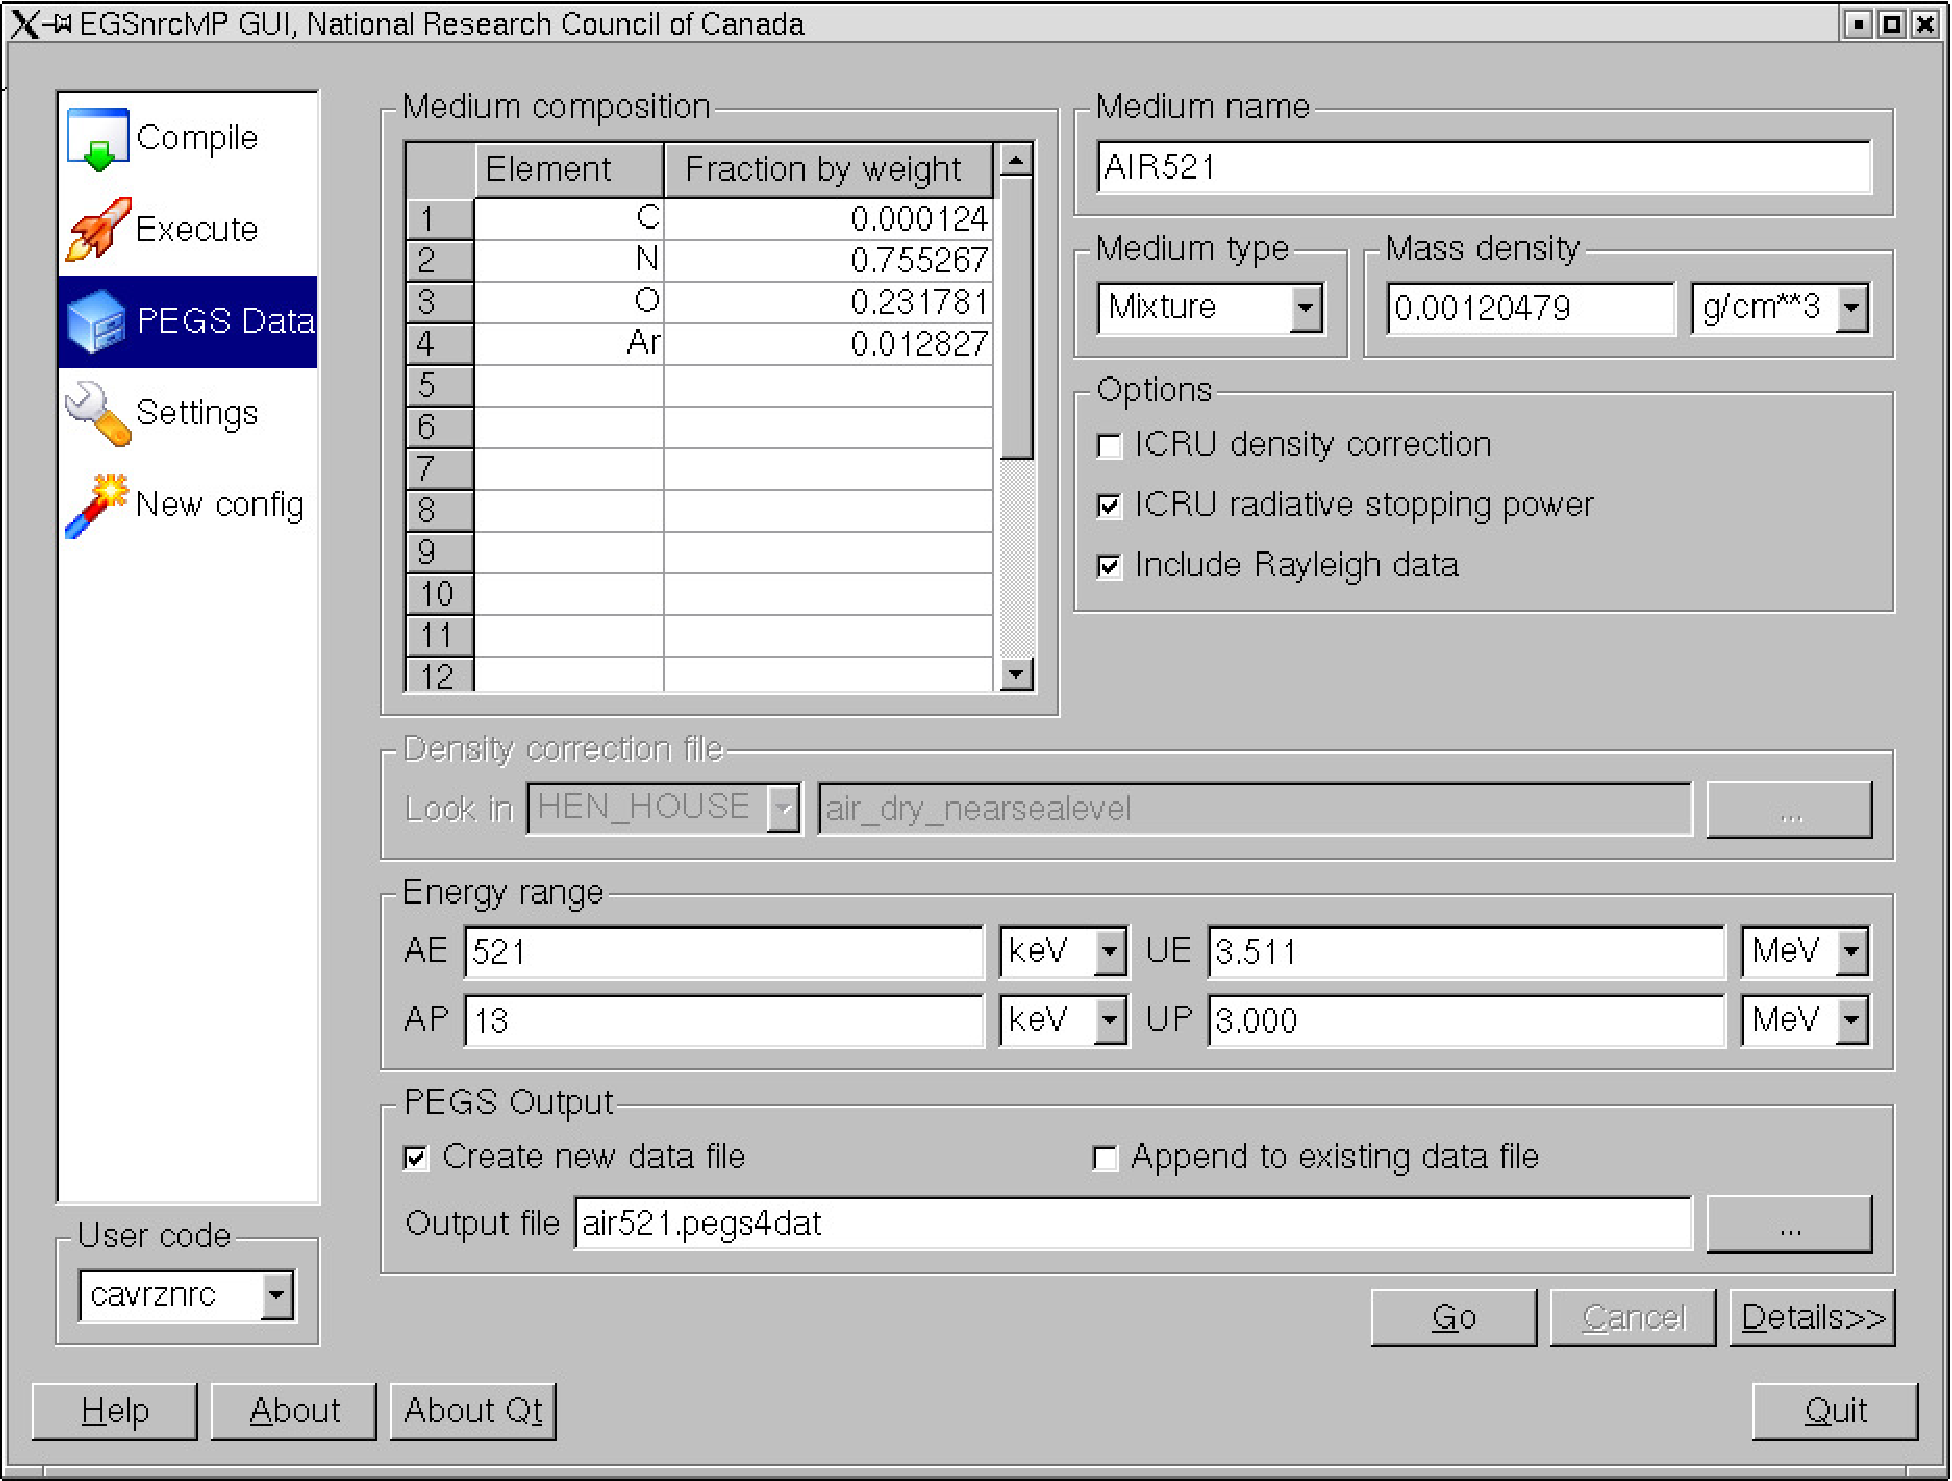
\includegraphics[width=12cm]{figures/egs_gui_pegs4_screen}
    \end{center}
   \caption{Screen shot of the {\tt egs\_gui} set to run PEGS4 to create
an air data set. Filling in this form is much easier than creating an input
file and access to the density effect corrections is easy. The GUI
does not allow any value except {\tt IUNRST = 0}. For details, see
PIRS-877\cite{Ka03}. }
   \label{fig_pegs4_screen}
\end{figure}

\subsection{Some new documentation}

\subsubsection{Photon data for EGSnrc}
\label{xsections}
Originally, EGS main field of application was high energy physics.
For this reason, no attention was paid to the accuracy of the
photon cross sections near atomic absorption edges\cite{RB90} and
PEGS4 was designed to generate a grid with a maximum number of photon
energy points, {\tt \$MXGE}, in the entire energy range requested by the user.
{\tt \$MXGE} is a macro which sets the array dimensions for the energy-dependent
photon data. Although {\tt \$MXGE} can be changed in the PEGS4 code,
PEGS4's algorithm for deciding how many bins to use might still pick many
fewer bins than {\tt \$MXGE}. The decision is based on the overall accuracy to
reproduce the cross sections in the entire energy interval.

\begin{figure}[hbtp]
\begin{center}
\includegraphics*[width=10.0cm]{figures/xcom_250keV_zoom}
\end{center}
\caption[Mean free path $\lambda$ for lead in the vicinity
of the L1 and L2 atomic absorption edges for two different
energy grids]
{Mean free path $\lambda$ for lead in the vicinity
of the L1 and L2 atomic absorption edges for two different
energy grids. Data sets generated by EGSnrc from
the XCOM cross section compilation for an energy range
10 keV to 250 keV.
}
\label{accuracy_xsections}
\end{figure}

Typical PEGS4 data sets used in radiotherapy
calculations are created for an energy range between 10 keV and 20 MeV.
If these data sets are used in the kilovoltage energy
range, inaccuracies in the cross section interpolation procedure near
absorption edges can potentially lead to errors in the calculations.
Fig. \ref{accuracy_xsections} shows two cross section data sets
for the same energy range (10 keV - 250 keV) when using
different energy grids (200 and 2000 bins). A coarser energy
grid will cause larger interpolation errors near the absorption edge.

EGSnrc default behavior has been set to ignore PEGS4 photon
data and recreate the photon cross sections using a logarithmic energy
grid with {\tt \$MXGE} energy points. However, EGSnrc still needs the
PEGS4 data file for material information, photon threshold energies
({\tt AP, UP}), and a fraction of the electron data.
By default data is read from the
Storm and Israel\cite{SI70} photon cross section compilation
({\tt si\_pair.data, si\_photo.data, si\_rayleigh.data and
si\_triplet.data}).
As alternative, EGSnrc offers such cross section data files
for the XCOM\cite{HS95} ({\tt xcom\_*.data}) and EPDL97\cite{Cu89}
({\tt epdl\_*.data}) photon cross section compilations.
New photon cross section compilations can be added following the
same format as above, \ie, {\tt prefix\_*.data}.
The choice of the photon cross section
compilation is done by input as shown in the example below:
\begin{verbatim}

  :start MC transport parameter:
      .                             # This entry is case sensitive
      Photon cross sections = xcom  # xcom, epdl, si(default) or any_prefix
      .
  :stop MC transport parameter:

\end{verbatim}
The prefix used is case sensitive and must be such that the required files
are available in the {\tt \$HEN\_HOUSE/data} directory.

Since the 2011 release (V4-r2-3-2) EGSnrc allows the
use of photon cross section data in the PEGS4 data file. This could
come in handy to compare with older calculations for validation
purposes. To accomplish this, one must set the photon cross section key to
{\tt pegs4} (case insensitive) as shown in the following input file snippet:
\begin{verbatim}

  :start MC transport parameter:
      .
      Photon cross sections = pegs4 # case insensitive
      .
  :stop MC transport parameter:

\end{verbatim}
\subsubsection{Some additional outputs- unrestricted cross sections}
The original version of PEGS4 contained a few undocumented options which
many people have made use of, so they are now documented here.  Basically
there is an additional parameter, {\tt IUNRST} which allows various stopping
powers to be calculated, rather than just the restricted stopping powers
normally calculated when {\tt IUNRST = 0}.  The {\tt IUNRST} input is made as part of
the namelist input for INP (along with NE, AE etc).  Basically {\tt IUNRST} gives
access to a variety of different stopping powers and allows for simulations
which model various types of CSDA calculations.
\begin{description}
\index{IUNRST}
\index{restricted stopping powers}
\index{unrestricted stopping powers}
\index{radiative stopping powers}
\index{collision stopping powers}
\item[IUNRST = 0, restricted stopping powers:] This is the default case
which is needed for normal simulations. The stopping powers output by PEGS4
are the restricted collision and radiative stopping powers.

\item[IUNRST = 1, unrestricted collision stopping power:] This is useful
for calculating unrestricted stopping powers for comparison to frequently
published values.

\item[IUNRST = 2, CSDA data set:] This produces a data set which can do one
form of CSDA calculation. The stopping power produced is the unrestricted
total (collision + radiative) stopping power and the distances to discrete
electron interactions is infinite (i.e. they never occur). A simulation
done with this data set is a form of CSDA calculation, with all of the
bremsstrahlung energy deposited locally.

\item[IUNRST = 3, CSDA calculation with brem interaction:] The stopping
powers are the sum of the unrestricted collision stopping power plus the
restricted stopping power and the distance to discrete interactions takes
into account only bremsstrahlung events.

\item[IUNRST = 4, CSDA calculation with delta-ray interactions:] The
stopping powers are the sum of the restricted collision stopping powers and
the unrestricted collision stopping powers and the distance to discrete
interactions takes into account only the creation of knock-on electrons
or delta-rays.

\item[IUNRST = 5, unrestricted radiative stopping power:] This complements
{\tt IUNRST = 1} and allows comparison to published radiative stopping powers.

\item[IUNRST = 6, restricted radiative stopping power:] Allows for direct
calculation of the restricted radiative stopping powers.

\item[IUNRST = 7, restricted collision stopping powers:] Allows for direct
calculation of the restricted collision stopping power.
\end{description}
Note that for low values of AP (e.g. 0.010 keV) the restricted radiative
collision stopping power is very close to zero and hence the stopping
powers with {\tt IUNRST = 0} are close to those for {\tt IUNRST = 7}.

The code EXAMIN (see section~\ref{examin}, page~\pageref{examin}) will take
the data sets produced by PEGS4 and print tables of cross section data
and/or plot these same data in user friendly units.
\index{EXAMIN}

\subsubsection{Use of ICRU Report 37 Collision Stopping Powers}
\label{icru37_csp}
\index{ICRU Report 37}
\index{collision stopping powers}
For very precise dosimetry work it is often advantageous to make use of
collision stopping powers recommended by the ICRU in their Report
37\cite{ICRU37}.  This option was added to PEGS4 in 1989\cite{Du89}.
Basically PEGS4 allows the user to read in a file which contains an arbitrary
density effect data set ($\delta$ values). The EGSnrc distribution
supplies the data sets
required for a large number of materials as calculated by Berger and
Seltzer\cite{BS83} for ICRU Report 37 (see
\verb+$HEN_HOUSE/pegs4/density_corrections+).
\index{Seltzer, Stephen} \index{Berger, Martin}

\index{PEGS4!EPSTFL}
\index{EPSTFL}
To implement this option, one adds {\tt EPSTFL=1} to the {\tt INP}
namelist input for the {\tt ELEM, COMP} or {\tt MIXT} option
and executes PEGS4 as:
\begin{verbatim}
pegs4.exe -i inputfile [-o ofile] [-a] [-d density] [-x crosssection] [-e HEN_HOUSE]

inputfile.pegs4inp   the input file
output defaults to $HEN_HOUSE/pegs4/data/inputfile.pegs4dat
                or, if ofile is given, to $HEN_HOUSE/pegs4/data/ofile.pegs4dat
[-a]            => append results to output file
[-d density]    => use density.density   for density effect
[-x crosssection] => use $HEN_HOUSE/pegs4/crosssection instead of
                                $HEN_HOUSE/pegs4/pgs4pepr.dat
[-e HEN_HOUSE]  => use this absolute location as the HEN_HOUSE
\end{verbatim}
where {\tt input1.pegs4inp} contains the standard PEGS4 input file (with
{\tt EPSTFL=1}) and {\tt  input2.density} is the file with the density effect
data needed.

PEGS4 verifies that the data in {\tt input2.density} corresponds to the same
material as described in {\tt input1.pegs4inp}, and in particular demands
that the densities match.  If you want to create a data set using the
density effect data for graphite based on a density of 2.26 g/cm$^3$ but
the real bulk data is 1.70 g/cm$^3$, you must edit the density effect file
and artificially change the density to match the bulk density you are
after, otherwise PEGS4 will stop.

Note that the density effect file also provides the ICRU 37 value of the I
value for the material and PEGS4 uses this rather than its internally
calculated value.

Data sets created with {\tt EPSTFL=1} and {\tt IUNRST = 1} should match the
collision stopping powers in ICRU Report 37 exactly.

\subsubsection{Use of ICRU Report 37 Radiative Stopping Powers}
\index{IAPRIM}
\index{radiative stopping powers}
\index{ICRU Report 37}
In 1989 an option was added to PEGS4\cite{Ro89a} which ensured that
the unrestricted radiative stopping powers calculated by PEGS4 were
identical to those calculated by Berger and Seltzer\cite{BS83} and
included in ICRU Report 37\cite{ICRU37}.  This was done by scaling the
cross sections used in PEGS4 to ensure that these stopping powers matched.
This made a significant difference to the bremsstrahlung cross sections
at low energies.  It is strongly recommended that this option always
be used and has been made the default value in PEGS4. To restore the
original PEGS4 values, enter  the input {\tt IAPRIM=0}
to the {\tt INP} namelist input for the {\tt ELEM, COMP} or {\tt MIXT}
option.
\index{PEGS4!IAPRIM}


Note that this change does not produce the same photon differential cross
sections as calculated by Seltzer and Berger\cite{SB85}, but this option
has been added to EGSnrc (see section~\ref{step_2}) and turned on by
setting {\tt ibr\_nist = 1}.
\index{ibr\_nist}



\subsubsection{A Bug in PEGS4}
\index{PEGS4!bug}
Although the PEGS4 manual reports that one may produce data sets for many
materials in one run, this is not in fact possible.  One must run the code
separately for each material desired and then concatenate these files into
one master file.

\newpage
\subsection{Original PEGS4 User Manual}
%\begin{center}
\index{Nelson, Ralph}
\index{Hirayama, Hideo}
\begin{verbatim}


                     SLAC265 - APPENDIX 3



                      PEGS4 User Manual






                              By


                       Walter R. Nelson
               Stanford Linear Accelerator Center
                      Stanford University
                   Stanford, CA 94305, U.S.A.


                        Hideo Hirayama
       National Laboratory for High Energy Physics (KEK)
            Oho-machi, Tsukuba-gun, Ibaraki, Japan


                      David W. O. Rogers
              National Research Council of Canada
                    Ottawa K1A 0R6, Canada



                       31 December 1985









      [This PEGS4 User Manual is based directly on Appendix 3 of
               SLAC-265, The EGS4 Code System]
\end{verbatim}



%\end{center}
%\end{center}
 \newpage \index{PEGS4!introduction} \begin{verbatim}
 A3.  PEGS4 USER MANUAL
 -----------------
 A3.1 Introduction
 -----------------

      The PEGS code (Preprocessor for EGS) is a stand alone
 utility program written in Mortran **.  PEGS' purpose is to
 generate material data for the EGS code, and to provide other
 services for the user who is studying or simulating electro-
 magnetic interactions.  The active operations of PEGS are
 functionals; that is, they are operations whose arguments are
 functions (the functions related to physics interactions).
 Included among these operations are:

      -  Fitting of functions by means of piecewise linear fits.

      -  Production of print plots of selected functions.

      -  Evaluation of functions at selected points.

      -  Comparision of functions with sampled spectra.


 Associated with these active functionals are other operations;
 namely,


      -  Selection of material to which the functions refer.

      -  Selection of energy cutoffs for fits.

      -  Punching of fit data.


 [Note: Those interested in preparing data sets for EGS4 can go
        directly to Section A3.3]

 ---------------
\end{verbatim}
{\tt   ** A. J. Cook, "Mortran3 User's Guide"\cite{Co83}.  Also, see
``An EGS Users Guide to Mortran3'' (section~\ref{UGM3}).}
\begin{verbatim}




 A3.1-1
\end{verbatim}
\newpage
\index{PEGS4!structure}
\begin{verbatim}
 ------------------------------------
 A3.2 Structural Organization of PEGS
 ------------------------------------
      The PEGS code contains over 4200 Mortran source lines
 which are the source for a MAIN program, BLOCK DATA subpro-
 gram, 12 subroutines, and 83 functions.  Despite the large
 number of subprograms, PEGS has a simple structure.  Fig.
 A3.2.1 shows a flowchart of the MAIN program of PEGS.  After
 the once-only initializations an option loop is entered.
 Each time through the option loop, an option is read (option
 names are four characters and are read as 4A1), numeric con-
 trol parameters are read (using NAMELIST/INP/), and then the
 option name is looked up in the option table.  If not found,
 the job is aborted.  If found, the appropriate code is exec-
 uted and return is passed to the beginning of the option
 loop.  Normal exit from the loop is by selection of the STOP
 option, or detection of an End of File condition on the con-
 trol input file.  The details for the use of the options are
 contained in Section A3.3.

      Fig. A3.2.2 shows the subprogram relationships of PEGS.
 Boxed items are subprograms, and labels for option names
 (i.e., :CALL:) are used to show which subprograms correspond to
 which options.  It can be seen that the physical routines are
 accessed directly for the PWLF option.  For utility options
 (TEST, PLTN, PLTI, HPLT, and CALL) the physical routines are
 referenced using the function FI---the so-called "function
 multiplexer".  Function FI has five arguments.  The first
 argument (I) tells which physical function to invoke, and the
 other four arguments (X1, X2, X3, X4) are used as needed as
 arguments for the called function.  FI then returns the value
 returned by the called function.

      This method of implementing options that are functionals
 was selected to avoid the necessity of having a separate call
 to the associated utility routines for each physical function
 on which it might be desired to operate.  It was also desired
 to be able to refer to the particular function symbolically,
 both at compile time and at run-time, and to know the number
 of arguments to each function.  In order to have these
 conveniences and also allow easy insertion or deletion of
 functions to the list of functions accessible to FI, a
 Mortran macro ($FUNCTIONS) was written which takes a
 list of names of functions (each of which is immediately pre-
 ceded by the number of arguments it has) and generates other
 macros containing the desired information.  In particular,
 A3.2-1
\end{verbatim}
\newpage
\index{PEGS4!flow chart}
\begin{center}
\begin{boxedverbatim}
                          +------+
                          | PEGS |
                          +------+
                            |  |       +-------------+
                initialize  |  +------>| OPTION LOOP |<-----+
             +--------------+          +-------------+      A
             |                                |             |
             |                                |             |
             V                                V             |
 +------------------------+          +-----------------+    |
 |   Compute Physical &   |          |   Read Option   |    |
 | Mathematical Constants |          |    Name (4A1)   |    |
 +------------------------+          |        &        |    |
             |                       |   Read Control  |    |
             |                       |    Parameters   |    |
             V                       | (NAMELIST/INP/) |    |
 +------------------------+          +-----------------+    |
 | Read Pair Production & |                   |             |
 |  Photo Cross Sections  |                   |             |
 |    from File PHPRDAT   |                   |             |
 +------------------------+                   |             |
                                              V             |
                +------+     Yes      +--------------+      |
                | Stop |<------------ | End of File? |      |
                +------+              +--------------+      |
                                              |             |
                                              | No          |
                                              |             |
                                              V             |
      +-----------------------+       +---------------+     |
      | Illegal Option---Stop |<----- | Select Option |     |
      +-----------------------+       +---------------+     |
                                              |             |
                                              |             |
                                              V             |
   +<---------------------------------------- +             |
   |                                                        |
   V                                                        |
   *                                                        *
  * *                                                      * *
 * 1 *                                                    * 2 *
  * *                                                      * *
   *                                                        *
      Fig. A3.2.1  Flowchart of the MAIN Program of PEGS
                        (continued on next page)
 A3.2-2
\end{boxedverbatim}
\end{center}
\newpage \index{PEGS4!flow chart}
\begin{center}
\begin{boxedverbatim}
   *                                                         *
  * *                                                       * *
 * 1 *                                                     * 2 *
  * *                                                       * *
   *                                                         *
   |          +-----------------------+                      ^
   +-->:ELEM: | Set Up Element Medium | -------------------> |
   |          +-----------------------+                      |
   |          +-----------------------+                      |
   +-->:MIXT: | Set Up Mixture Medium | -------------------> |
   |          +-----------------------+                      |
   |          +------------------------+                     |
   +-->:COMP: | Set Up Compound Medium | ------------------> |
   |          +------------------------+                     |
   |          +------------------------+                     |
   +-->:ENER: | Set Energy Cutoffs and | ------------------> |
   |          | Compute Thresholds     |                     |
   |          +------------------------+                     |
   |          +---------------------+                        |
   +-->:PLTN: | Plot Named Function | ---------------------> |
   |          +---------------------+                        |
   |          +-----------------------+                      |
   +-->:PLTI: | Plot Indexed Function | -------------------> |
   |          +-----------------------+                      |
   |          +-----------------------+                      |
   +-->:HPLT: | Histogram Theoretical | -------------------> |
   |          |  vs Sampled Spectrum  |                      |
   |          +-----------------------+                      |
   |          +-------------------------+                    |
   +-->:CALL: | Evaluate Named Function | -----------------> |
   |          +-------------------------+                    |
   |          +-----------------------------+                |
   +-->:TEST: | Plot Functions To Be Fitted | -------------> |
   |          +-----------------------------+                |
   |          +----------------------+                       |
   +-->:PWLF: | Piecewise Linear Fit | --------------------> |
   |          +----------------------+                       |
   |          +------------------------+                     |
   +-->:DECK: | Punch Deck of Material | ------------------> +
   |          | Dependent Data         |
   |          +------------------------+
   |          +------+
   +-->:STOP: | Stop |
              +------+
      Fig. A3.2.1  Flowchart of the MAIN Program of PEGS
                     (continued from previous page)
 A3.2-3
\end{boxedverbatim}
\end{center}
\newpage \index{PEGS4!subprograms}
\begin{center}
\begin{boxedverbatim}
     +------------+         +------+
     | BLOCK DATA |         | MAIN |
     +------------+         +------+
                                |
     + --- + -- + ----- + ----- + ----- + ----- + ---- + ---- +
     |     |            |       |       |       |      |      |
     |     |         :PWLF:  :DECK:  :TEST:  :HPLT: :CALL: :ENER:
     |     |            |       |    :PLTN:     |      |
     |     |            |     +---+  :PLTI:  +-----+   |
     |     |            |     |LAY|     |    |HPLT1|   |
     |     |            |     +---+     |    +-----+   |
     |     |            |            +----+     |      |
  +------+ |        +---+----+       |PLOT|     |      |
  |PMDCON| |        |        |       +----+     |      |
  +------+ |     +-----+  +-----+       |       |      |
           |     |EBIND|  |PWLF1|       +-----> | <--- +
           |     +-----+  +-----+               |
        :ELEM:               |                  |
        :MIXT:            +----+                |
        :COMP:            |QFIT|                *
           |              +----+               * *
   + ----- + ----- +         |                * 3 *
   |       |       |         |                 * *
 +---+ +------+ +------+     |                  *
 |MIX| |SPINIT| |DIFFER|     |
 +---+ +------+ +------+     |
                        + -- + -- + --------------- +
                        |         |                 |
                     +-----+   +-----+           +-----+
                     |EFUNS|   |GFUNS|           |RFUNS|
                     +-----+   +-----+           +-----+
                        |         |                 |
    +-----+----+-----+--+---+---+ |   +------+   +-----+
    |     |    |     |      |   | +---|PHOTTE|   |AINTP|
 +------+ | +------+ | +------+ | |   +------+   +-----+
 |SPTOTP| | |ANIHTM| | |BHABTM| | |   +------+
 +------+ | +------+ | +------+ | +---|COMPTM|
          |          |          | |   +------+
 +------+ | +------+ | +------+ | |   +------+
 |SPTOTE|-+ |AMOLTM|-+ |BREMTM|-+ +---|PAIRTU|
 +------+   +------+   +------+   |   +------+
                                  |   +------+
                                  +---|COHETM|
                                      +------+
      Fig. A3.2.2  Subprogram Relationships of PEGS
                      (continued on next page)
 A3.2-4
\end{boxedverbatim}
\end{center}
\newpage \index{PEGS4!subroutines}
\begin{center}
\begin{boxedverbatim}
                               *
                              * *
                             * 3 *
                              * *
                               *
                               |
                               |
                               |
                               |
                  + ---------------------- +
                  |           FI           |
                  | "Function Multiplexer" |
                  + ---------------------- +
                               |
                               |
                               |
           + ------------------------------------- +
           |                                       |
           |   ALIN     APRIM    COMPFM   PAIRTE   |
           |   ALINI    BHABDM   COMPRM   PAIRTM   |
           |            BHABFM   COMPTM   PAIRTR   |
           |   ADFMOL   BHABRM   CRATIO   PAIRTU   |
           |   ADIMOL   BHABTM   EBIND    PAIRTZ   |
           |   ADDMOL   BREMDR   EBR1     PBR1     |
           |   ALOG     BREMFR   EDEDX    PBR2     |
           |   EXP      BREMDZ   ESIG     PDEDX    |
           |   AREC     BRMSDZ   FCOULC   PHOTTZ   |
           |   ALKE     BREMFZ   GBR1     PHOTTE   |
           |   ALKEI    BRMSFZ   GBR2     PSIG     |
           |   AMOLDM   BREMRR   GMFP     SPIONE   |
           |   AMOLFM   BREMRM   PAIRDR   SPIONP   |
           |   AMOLRM   BREMRZ   PAIRFR   SPTOTE   |
           |   AMOLTM   BREMTM   PAIRDZ   SPTOTP   |
           |   ANIHDM   BREMTR   PAIRFZ   TMXB     |
           |   ANIHFM   BRMSRM   PAIRRM   TMXS     |
           |   ANIHRM   BRMSRZ   PAIRRR   TMXDE2   |
           |   ANIHTM   BRMSTM   PAIRRZ   XSIF     |
           |            COHETM                     |
           |            COHETZ                     |
           |            COMPDM                     |
           + ------------------------------------- +

      Fig. A3.2.2  Subprogram Relationships of PEGS
                   (continued from previous page)


 A3.2-5                                                       .
\end{boxedverbatim}
\end{center}
\newpage \index{PEGS4!macros} \begin{verbatim}
 the following macros are defined:

      $NFUNS  -  Gives the number of functions.

      $FLIST$DATA(FNAME)  -  Generates a data statement init-
      ializing the array FNAME(6,$NFUNS) so that FNAME(i,j) has
      the ith character of the name of the jth function.

      $FLIST$NARGS  -  Gives a list of the number of arguments
      for each function, which is used to initialize the run-
      time array NFARG($NFUNS).

      $FLIST$FNUMS  -  Gives a list of numbers from 1 to
      $NFUNS, which is used to generate the computed GO TO
      in FI.

      $FLIST$FCALLS  -  Generates the function calls in FI with
      the proper number of arguments for each function taken
      from the list X1, X2, X3, X4.

      $FN(function name)  -  Gives the function index of the
      specified function.

      $NA(function name)  -  Gives the number of arguments for
      the specified function.


      It should also be noted that there are relationships
 between the functions shown in Fig. A3.2.2 that are not
 indicated there.  We show the most complicated of these in
 Figs. A3.2.3a,b (Bremsstrahlung Related Functions) and in
 Figs. A3.2.4a,b (Pair Production Related Functions).  One
 reason for the complexity of these is that the higher level
 forms of the cross sections must be obtained by numerical
 integration of the more differential forms.











 A3.2-6
\end{verbatim}
\newpage \index{PEGS4!functions}
\begin{center}
\begin{boxedverbatim}
                        +------+
                        |BREMTM|
                        +------+
                            |
                            V
                        +------+
                        |BREMRM|
                        +------+
                            |
                            V
 +------+               +------+  initialize   +------+
 |  QD  |<------------- |BREMRZ|-------------> |BREMDZ|
 +------+               +------+    BREMFZ     +------+
    |                                              |
    V                                              |
 +------+                                          |
 |DCADRE|                                          |
 +------+                                          |
    |                                              |
    V                                              V
 +------+               +------+               +------+
 |BREMFZ|-------------> |BRMSFZ|<------------- |BRMSDZ|
 +------+               +------+               +------+
                            A                    A |
                            |                    | |   +------+
            +---------------+                    | +-->|APRIM |
            |                                    | |   +------+
        +------+        +------+   initialize    | |
        |DCADRE|   +----|BRMSRZ|---------------> + |   +------+
        +------+   |    +------+     BRMSFZ        +-->| XSIF |
            A      |        A                      |   +------+
            |      |        |                      |
        +------+   |    +------+                   |   +------+
        |  QD  |<--+    |BRMSRM|                   +-->|FCOULC|
        +------+        +------+                       +------+
                            |
   +------+             +------+             +------+
   |SPTOTE|-----------> |BRMSTM|<----------- |SPTOTP|
   +------+             +------+             +------+
      |                                          |
      V                                          V
   +------+             +------+             +------+
   |SPIONE|-----------> |SPIONB|<----------- |SPIONP|
   +------+             +------+             +------+
Fig. A3.2.3a  Bremsstrahlung Related Functions---Most Accurate Form
   (Used to Produce the Total Cross Sections and Stopping Power).
 A3.2-7
\end{boxedverbatim}
\end{center}
\newpage \index{PEGS4!functions}
\begin{center}
\begin{boxedverbatim}




                             +------+
                             |BREMTR|
                             +------+
                                 |
                                 |
                                 V
                             +------+
                             |BREMRR|
                             +------+
                                 |
                                 |
                      initialize V
                     + <---------+--------> +
                     |  BREMFR              |
                     |                      |
                     V                      V
                  +------+              +------+
                  |BREMDR|              |  QD  |
                  +------+              +------+
                     |                      |
                     |                      |
                     |                      V
                     |                  +------+
                     |                  |DCADRE|
                     |                  +------+
                     |                      |
                     |                      |
                     |                      |
                     |       +------+       |
                     + ----> |BREMFR| <---- +
                             +------+


     Fig. A3.2.3b  Bremsstrahlung Related Functions---With Run-
                     Time Approximations (For Comparison
                           with Sampled Spectra).






 A3.2-8
\end{boxedverbatim}
\end{center}
\newpage \index{PEGS4!functions}
\begin{center}
\begin{boxedverbatim}




                         +------+
                         |PAIRTU|
                         +------+
                           |  |
    + <------------------- +  + -------------------> +
    |                                                |
    V                                                V
 +------+                                        +------+
 |PAIRTM|                                        |PAIRTE|
 +------+                                        +------+
    |                                                |
    V                                                V
 +------+                                        +------+
 |PAIRRM|                                        |PAIRTZ|
 +------+                                        +------+
    |                                                |
    V                                                V
 +------+   initialize                           +------+
 |PAIRRZ|-------------> +                        |AINTP |
 +------+     PAIRFZ    |                        +------+
    |                   |
    |                   |
    |                   |
    |                   |
    V                   V
 +------+            +------+            +------+
 |  QD  |            |PAIRDZ|-----+----> | XSIF |
 +------+            +------+     |      +------+
   |                    |         |
   |                    |         |      +------+
   |                    |         +----> |FCOULC|
   V                    V                +------+
 +------+            +------+
 |DCADRE|----------> |PAIRFZ|
 +------+            +------+


     Fig. A3.2.4a  Pair Production Related Functions---Most
                  Accurate Form (Used to Produce the Total
                  Cross Sections and Stopping Power).


 A3.2-9
\end{boxedverbatim}
\end{center}
\newpage \index{PEGS4!functions}
\begin{center}
\begin{boxedverbatim}



                             +------+
                             |PAIRTR|
                             +------+
                                 |
                                 |
                                 V
                             +------+
                             |PAIRRR|
                             +------+
                                 |
                                 |
                      initialize V
                     + <-------- + -------> +
                     |  PAIRFR              |
                     |                      |
                     V                      V
                  +------+              +------+
                  |PAIRDR|              |  QD  |
                  +------+              +------+
                     |                      |
                     |                      |
                     |                      V
                     |                  +------+
                     |                  |DCADRE|
                     |                  +------+
                     |                      |
                     |                      |
                     |                      |
                     |       +------+       |
                     + ----> |PAIRFR| <---- +
                             +------+


     Fig. A3.2.4b  Pair Production Related Functions---With
                  Run-Time Approximations (For Comparison
                  with Sampled Spectra).







 A3.2-10
\end{boxedverbatim}
\end{center}
\newpage \index{PEGS4!subroutines} \begin{verbatim}
      Table A3.2.1 lists the SUBROUTINES used in PEGS.  A brief
 description of their use and page references for a fuller
 discussion is given.

      Table A3.2.2 lists the FUNCTIONS used in PEGS along with
 their mathematical symbols, definitions, and locations in this
 report for a fuller discussion.  The names of most of the
 functions have been chosen in a rather mnemonic way.  The
 first three or four letters suggest the process being con-
 sidered.  The last letter designates the form of the cross
 section (Z for element, M for mixture, and R for "run-time"
 mixture).  The next to last letter describes either the part-
 icular form of the cross section (such as D for differential,
 T for total or R for range-integrated), or it indicates that
 only the secondary energy is to vary, with other data being
 passed through a common.  The letter F is used in such cases
 and the data in common is initialized using the corresponding
 function that has a next to last letter of D.  If the function
 word begins with an I through N (i.e., the FORTRAN integer
 convention) the word is prefixed with the letter A.  A few
 examples are given below:


    AMOLDM is the differential Moller cross section for a
           mixture of elements.

    BREMDR is the differential bremsstrahlung cross section
           for a "run-time" mixture of elements.

    BREMRM is the bremsstrahlung cross section, integrated
           over some energy range, for a mixture of elements.

    BRMSTM is the soft bremsstrahlung total cross section for
           a mixture of elements.

    PAIRRR is the pair production cross section, integrated
           over some energy range, for a "run-time" mixture
           of elements.

    PAIRTZ is the total cross section for pair production
           for an element.

      This method of naming is not strictly adhered to,
 however.  For example, SPIONE is the ionization stopping
 power for an electron, PBR1 and PBR2 are positron branching
 ratios, and GMFP is the gamma-ray mean free path.
 A3.2-11
\end{verbatim}
\newpage \index{PEGS4!subroutines} \begin{verbatim}
                         Table A3.2.1
                   SUBROUTINES Used In PEGS
 -----------------------------------------------------------------
    NAME                 DESCRIPTION                   PAGES
 -----------------------------------------------------------------
    DIFFER    Determines the various parameters       A3.2-4,
              needed for bremsstrahlung and pair      A3.3-11
              production energy sampling.

    EFUNS     Subprogram to compute electron          A3.2-4
              functions to be fit in a way
              that avoids repetition.

    GFUNS     Subprogram to compute photon            A3.2-4
              functions to be fit in a way
              that avoids repetition.

    HPLT1     Creates line printer plot comparisons   A3.2-4,
              of EGS-sampled data (UCTESTSR User      A3.3-20,21
              Code) and theoretical functions of PEGS.

    LAY       Subprogram to produce a deck of         A3.2-4,
              material dependent data (for sub-       A3.3-17
              sequent use by EGS).

    MIX       Computes Z-dependent paramaters         A3.2-4,
              that reside in COMMON/MOLVAR/.          A3.3-11

    MOLIER    Computes material independent           A3.2-4
              multiple scattering data (EGS2 only!).

    PLOT      Subprogram to plot a given function     A3.2-4
              (referenced by number).

    PMDCON    Determines the physical, mathematical,  A3.2-4
              & derived constants in a mnemonic way.

    PWLF1     Subprogram to piecewise linearly fit    A3.2-4,19,
              up to 10 functions simultaneously on    A3.3-14
              an interval (XL,XU).

    RFUNS     Subprogram to compute Rayleigh          A3.2-4
              scattering functions to be fit in
              a way that avoids repetition.
    SPINIT    Initializes stopping power functions    A3.2-4,
              for a particular medium.                A3.3-11
 A3.2-12
\end{verbatim}
\newpage  \index{PEGS4!functions} \begin{verbatim}


                         Table A3.2.2

                   FUNCTIONS Used In PEGS


 -----------------------------------------------------------------
    NAME                 DESCRIPTION                   PAGES
 -----------------------------------------------------------------
    AFFACT    Atomic form factor (squared) for an
              element or mixture of elements.

    AINTP     Linear or log interpolation function.   A3.2-4,9

    ALKE      Log of kinetic energy (ALOG(E-RM)),     A3.2-5,
              used as a cumulative distribution       A3.3-20
              function for fits and plots.

    ALKEI     Inverse of ALKE (=EXP(X)+RM).           A3.2-5

    ALIN      Linear cumulative distribution func-    A3.2-5,
              tion for plots (ALIN(X)=X).             A3.3-20

    ALINI     Inverse of ALIN (=same as ALIN).        A3.2-5
              Used as inverse cumulative distri-
              bution function in plots.

    ADFMOL    Approximate cumulative distribution     A3.2-5,
              function for Moller and Bhabha cross    A3.3-20
              sections (ADFMOL(E)=-1/(E-RM)).

    ADIMOL    Inverse of ADFMOL.                      A3.2-5

    ADDMOL    Derivative of ADFMOL.                   A3.2-5

    AMOLDM    Moller differential cross section for   A3.2-5,11,14
              a mixture of elements.






                   (continued on next page)
 A3.2-13
\end{verbatim}
\newpage \index{PEGS4!functions} \begin{verbatim}


                         Table A3.2.2
                         (continued)


                   FUNCTIONS Used In PEGS

 -----------------------------------------------------------------
    NAME                 DESCRIPTION                   PAGES
 -----------------------------------------------------------------
    AMOLFM    "One argument" form of AMOLDM.          A3.2-5

    AMOLRM    Moller cross section, integrated over   A3.2-5
              some energy range, for a mixture of
              elements.

    AMOLTM    Moller total cross section for a        A3.2-4,5
              mixture of elements.

    ANIHDM    Annihilation differential cross         A3.2-5
              section for a mixture of elements.

    ANIHFM    "One argument" form of ANIHDM.          A3.2-5

    ANIHRM    Annihilation cross section, integrated  A3.2-5
              over some energy range, for a mixture
              of elements.

    ANIHTM    Annihilation total cross section for    A3.2-4,5
              a mixture of elements.

    APRIM     Empirical correction factor in          A3.2-5,7
              bremsstrahlung cross section.

    AREC      Reciprocal function (=derivative of     A3.2-5
              ALOG(X)).  Used as probability density
              function in log plots (AREC(X)=1/X).

    BHABDM    Bhabha differential cross section for   A3.2-5
              a mixture of elements.

    BHABFM    "One argument" form of BHABDM.          A3.2-5


                   (continued on next page)
 A3.2-14
\end{verbatim}
\newpage  \index{PEGS4!functions}\begin{verbatim}

                         Table A3.2.2
                         (continued)

                   FUNCTIONS Used In PEGS
 -----------------------------------------------------------------
    NAME                 DESCRIPTION                   PAGES
 -----------------------------------------------------------------
    BHABRM    Bhabha cross section, integrated over   A3.2-5
              some energy range, for a mixture of
              elements.

    BHABTM    Bhabha total cross section for a        A3.2-4,5
              mixture of elements.

    BREMDR    Bremsstrahlung differential cross       A3.2,5,8,11
              section for a "run-time" mixture
              of elements.

    BREMFR    "One argument" form of BREMDR.          A3.2-5,8

    BREMDZ    Bremsstrahlung differential cross       A3.2-5,7
              section for an element.

    BREMFZ    "One argument" form of BREMDZ.          A3.2-5,7

    BREMRM    Bremsstrahlung cross section, inte-     A3.2-5,7,11
              grated over some energy range, for a
              mixture of elements.

    BREMRR    Bremsstrahlung cross section, inte-     A3.2-5,8
              grated over some energy range, for a
              "run-time" mixture of elements.

    BREMRZ    Bremsstrahlung cross section, inte-     A3.2-5,7
              grated over some energy range, for an
              element.

    BREMTM    Bremsstrahlung total cross section      A3.2-4,5,7
              for a mixture of elements.

    BREMTR    Bremsstrahlung total cross section      A3.2-5,8
              for a "run-time" mixture of elements.

                   (continued on next page)
 A3.2-15
\end{verbatim}
\newpage  \index{PEGS4!functions}\begin{verbatim}
                        Table A3.2.2
                         (continued)
                   FUNCTIONS Used In PEGS
 -----------------------------------------------------------------
    NAME                 DESCRIPTION                   PAGES
 -----------------------------------------------------------------
    BRMSDZ    Soft bremsstrahlung differential        A3.2-5,7
              cross section for an element.

    BRMSFZ    "One argument" form of BRMSDZ.          A3.2-5,7

    BRMSRM    Soft bremsstrahlung cross section,      A3.2-5,7
              integrated over some energy range, for
              a mixture of elements.

    BRMSRZ    Soft brems cross section integrated     A3.2-5,7,
              over an energy range,for an element.    A3.3-19,20

    BRMSTM    Soft bremsstrahlung total cross         A3.2-5,7,11
              section for a mixture of elements.

    COHERTM   Coherent (Rayleigh) total cross         A3.2-4,5
              section for a mixture of elements.

    COHETZ    Coherent (Rayleigh) total cross         A3.2-5
              section for an element.

    COMPDM    Compton differential cross section      A3.2-5
              for a mixture of elements.

    COMPFM    "One argument" form for COMPDM.         A3.2-5

    COMPRM    Compton cross section, integrated over  A3.2-5
              an energy range, for a mixture of elements.

    COMPTM    Compton total cross section for a       A3.2-4,5
              mixture of elements.

    CRATIO    Coherent (Rayleigh) cross section ratio A3.2-5

    DCADRE    Quadrature routine to integrate f(x)    A3.2-7-10,19
              from a->b by cautious Romberg extrapolation.

    EBIND     Function to get an average photo-       A3.2-4,5
              electric binding energy.
                   (continued on next page)
 A3.2-16
\end{verbatim}
\newpage \index{PEGS4!functions} \begin{verbatim}
                        Table A3.2.2
                         (continued)

                   FUNCTIONS Used In PEGS
 -----------------------------------------------------------------
    NAME                 DESCRIPTION                   PAGES
 -----------------------------------------------------------------

    EBR1      Function to determine the electron(-)   A3.2-5
              branching ratio (Brem/Total).

    EDEDX     Evaluates SPTOTE with cutoff energies   A3.2-5
              of AE and AP.

    ESIG      Determines the total electron(-)        A3.2-5
              interaction cross section (prob-
              ability per radiation length).

    FCOULC    Coulomb correction term in pair         A3.2-5,7,9
              production and bremsstrahlung cross
              sections.

    FI        Function multiplexer.                   A3.2-1,5,6

    GBR1      Function to determine the gamma-ray     A3.2-5
              branching ratio (Pair/Total).

    GBR2      Function to determine the gamma-ray     A3.2-5
              branching ratio ((Pair+Compton)/Total).

    GMFP      Function to determine the gamma-ray     A3.2-5,11,
              mean free path.                         A3.3-18,19

    IFUNT     Given PEGS function name, it looks it
              up name in table and returns the
              function index.  Used by options that
              specify functions by name.

    PAIRDR    Pair production differential cross      A3.2-5,10,18
              section for a "run-time" mixture of
              elements.

    PAIRDZ    Pair production differential cross      A3.2-5,9,18
              section for an element.

                   (continued on next page)
 A3.2-17
\end{verbatim}
\newpage \index{PEGS4!functions} \begin{verbatim}
                         Table A3.2.2
                         (continued)
                   FUNCTIONS Used In PEGS
 -----------------------------------------------------------------
    NAME                 DESCRIPTION                   PAGES
 -----------------------------------------------------------------
    PAIRFR    "One argument" form of PAIRDR.          A3.2-5,10
    PAIRFZ    "One argument" form of PAIRDZ.          A3.2-5,10

    PAIRRM    Pair production cross section, inte-    A3.2-5,9
              grated over some energy range, for a
              mixture of elements.

    PAIRRR    Pair production cross section, inte-    A3.2-5,10,11
              grated over some energy range, for a
              "run-time" mixture of elements.

    PAIRRZ    Pair production cross section, inte-    A3.2-5,9
              grated over energy range, for element.

    PAIRTE    "Empirical" total pair production       A3.2-5,9
              production cross section for a
              mixture (=SUM(PZ(I)*PAIRTZ(Z(I))).

    PAIRTM    Pair production total cross section     A3.2-5,9
              for a mixture of elements, obtained
              by numerical integration of differ-
              ential cross section.

    PAIRTR    Pair production total cross section     A3.2-5,10
              for a "run-time" mixture of elements.

    PAIRTU    Pair production total cross section     A3.2-4,5,9
              actually "used".  Same as PAIRTE for
              primary energy less than 50 MeV;
              otherwise, same as PAIRTM.

    PAIRTZ    Computes contribution to empirical      A3.2-5,9,11
              pair production total cross section
              for an element assuming one atom per
              molecule.  It is obtained by log-linear
              interpolation of Israel-Storm data.

    PBR1      Function to determine the positron      A3.2-5,11
              branching ratio (Brem/Total).
                   (continued on next page)
 A3.2-18
\end{verbatim}
\newpage \index{PEGS4!functions} \begin{verbatim}
                         Table A3.2.2
                         (continued)
                   FUNCTIONS Used In PEGS
 -----------------------------------------------------------------
    NAME                 DESCRIPTION                   PAGES
 -----------------------------------------------------------------
    PBR2      Function to determine the positron      A3.2-5,11
              branching ratio ((Brem+Bhabha)/Total).

    PDEDX     Evaluates SPTOTP with cutoff energies   A3.2-5
              of AE and AP.

    PHOTTE    Determines the proper mix of PHOTTZ's   A3.2-4,5
              for a mixture.

    PHOTTZ    Determines the interpolated total       A3.2-5
              photoelectric cross section from
              tabulated data.

    PSIG      Determines the total positron           A3.2-5
              interaction cross section (prob-
              ability per radiation length).

    QD        Driver function for DCADRE, the         A3.2-7-10
              numerical integration routine.

    QFIT      Utility logical function for the        A3.2-4,
              piecewise linear fit subroutine, PWLF1. A3.3-14,15
              It returns .TRUE. if a given parti-
              tion gives a good fit.

    SPIONB    Does the work for SPIONE and SPIONP.    A3.2-7
              One argument tells whether to compute
              stopping power for electron or positron.

    SPIONE    Calculates the stopping power due to    A3.2-5,7
              ionization for electrons(-).

    SPIONP    Calculates the stopping power due to    A3.2-5,7
              ionization for positrons.

    SPTOTE    Calculates the total stopping power     A3.2-4,5,7
              (ionization plus soft bremsstrahlung)
              for electrons(-) for specified cutoffs.

                   (continued on next page)
 A3.2-19
\end{verbatim}
\newpage  \index{PEGS4!functions}\begin{verbatim}


                         Table A3.2.2
                         (continued)

                   FUNCTIONS Used In PEGS

 -----------------------------------------------------------------
    NAME                 DESCRIPTION                   PAGES
 -----------------------------------------------------------------
    SPTOTP    Calculates the total stopping power     A3.2-4,5,7,19
              (ionization plus soft bremsstrahlung)
              for positrons for specified cutoffs.

    TMXB      Determines the maximum total step       A3.2-5
              length consistent with Bethe's
              criterion.

    TMXS      Determines the minimum of TMXB and      A3.2-5
              10 radiation lengths.

    TMXDE2    Included for possible future modifi-    A3.2-5
              cation purposes (=TMXB/(E**2*BETA**4)).
              It might be easier to fit this quantity
              than to fit TMXB and then apply the
              the denominator in EGS at run-time.

    XSIF      Function to account for bremsstrahlung  A3.2-5,7,9
              and pair production in the field of
              the atomic electrons.

    ZTBL      Given the atomic symbol for an element,
              it returns the atomic number.













 A3.2-20                                                APPENDIX 3
\end{verbatim}
\newpage \index{PEGS4!options} \index{PEGS4!inputs}
\index{PEGS4!ELEM option}  \index{PEGS4!COMPT option} \index{PEGS4!MIXT option}
\label{pegs4_input}
\begin{verbatim}
 ------------------------------------------
 A3.3 PEGS Options and Input Specifications
 ------------------------------------------
    -------------------------------------
    A3.3.1 Interrelations Between Options
    -------------------------------------

      Fig. A3.3.1 illustrates the logical relationship between options of
PEGS.  For example, in order to be able to use the PLTN option, one of the
material specification options (ELEM, MIXT, COMP) must have already been
processed.  The PWLF option requires that both the ENER option and one of
the material specification options precede it.  To use the DECK option, it
is sufficient to have validly invoked the PWLF option.  The STOP and MIMS
options are seen to be independent of the others.

      In the following sections, for each option we will give its function,
parameters which control it, the format of cards needed to invoke it, and
an explanation of the routines (if any) that are used to implement it.  The
cards for a given option are named with the first part of their name being
the option name, and the last part the card number.  For example, MIXT2 is
the name of the second card needed for the MIXT option.  The information is
summarized in Table A3.3.1.  It should be noted that IBM and CDC require
different formats for NAMELIST data.  Also, the single card referred to as
being read by NAMELIST may in fact be several cards, provided that the
proper convention for continuing NAMELIST cards is followed.  Once the
first card (indicating the option) has been read in, however, the second
card (i.e., NAMELIST/INP/) must follow (see examples at the end of Section
A3.3.2).  We will use the IBM form of NAMELIST in our examples.

 -----------------------------------
 A3.3.2 The ELEM, MIXT, COMP Options
 -----------------------------------

      The purpose of the ELEMent, MIXTure, and COMPound options is to
specify the material used by the PEGS functions.  The parameters needed to
specify a material are its density (RHO), the number of different kinds of
atoms (NE), and, for each different kind of atom, its atomic number (Z(I)),
its atomic weight (WA(I)), and its proportion either by number (PZ(I)) for
a compound or by weight (RHOZ(I)) for a mixture.  PEGS has tables for the
atomic symbol (ASYMT(1:100)) and the atomic weight (WATBL(1:100)) for
elements I=1 through I=100, so the type of atom is specified by giving its
atomic symbol (ASYM(I)).  PEGS also has a table of the densities of the
elements (RHOTBL(1:100)).  Rayleigh (coherent) scattering data will be
appended to the normal output data if the IRAYL flag is set to 1 in
NAMELIST/INP/.

 A3.3-1
\end{verbatim}
\newpage \index{PEGS4!options}
\begin{center}
\begin{boxedverbatim}


   +------+    +------+    +------+          +------+
   |:ELEM:|    |:MIXT:|    |:COMP:|          |:ENER:|
   +------+    +------+    +------+          +------+
       |          |           |                  |
       |          |           |                  |
       |          |           |                  |
       |          V           |                  |
       |                      |                  |
       + ------> OR <-------- +                  |
                                                 |
                  |                              V
                  |
                  +---------------------------> AND ----+
                  |                                     |
                  |                              |      |
                  V                              |      |
    + -------+----+----+------- +                |      |
    |        |         |        |                |      |
    |        |         |        |                |      |
    V        V         V        V                |      |
 +------+ +------+ +------+ +------+ +------+    |      |
 |:PLTN:| |:PLTI:| |:HPLT:| |:CALL:| |:TEST:|<---+      |
 +------+ +------+ +------+ +------+ +------+           |
                                                        |
                                                        V
                                                     +------+
                                                     |:PWLF:|
 +------+                                            +------+
 |:MIMS:|                                               |
 +------+                                               |
                                                        V
 +------+                                            +------+
 |:STOP:|                                            |:DECK:|
 +------+                                            +------+





           Fig. A3.3.1  Logical Relationship Between
                       the Options of PEGS



 A3.3-2                                                 APPENDIX 3
\end{boxedverbatim}
\end{center}
\newpage \index{PEGS4!inputs}\index{ISSB} \begin{verbatim}
                         Table A3.3.1
                     PEGS Control Cards
 -----------------------------------------------------------------------
  CARD    FORMAT    VARIABLES READ          COMMENTS
 -----------------------------------------------------------------------
  ELEM1   (4A1)        OPT(1:4)    'ELEM'.  Means "select mat-
                                   erial that is an element."

  ELEM2 NAMELIST/INP/    RHO       Optional.  If given, this
                                   over-rides the PEGS default
                                   density (g/cm**3) for the element.

                         WA(1)     Optional.  Atomic weight of
                                   element.  If given, this
                                   over-rides the PEGS default.
                        IRAYL      Optional.  Set to unity to

                                   included Rayleigh output.

                        IUNRST     Optional.  Set to unity for
                                   unrestricted collision stopping power.

                        ISSB       Optional.  Set to unity to
                                   use own density effect param-
                                   eters (see text below).
                        GASP       Optional. See MIXT or COMP

  ELEM3 (24A1,       MEDIUM(1:24)  Identifier assigned to data
         6X,24A1)                  set to be produced.

                     IDSTRN(1:24)  Optional.  Identifer of
                                   medium name under which
                                   desired Sternheimer-Seltzer-
                                   Berger coeffcients are given
                                   in PEGS.  If not specified,
                                   identifier in MEDIUM(1:24) is used.

  ELEM4 (24(A2,1X))    ASYM(1)     Atomic symbol for element.
 -----------------------------------------------------------------------
  COMP1   (4A1)        OPT(1:4)    'COMP'.  Means "select mat-
                                   erial that is a compound."

  COMP2 NAMELIST/INP/    NE        Number of elements in compound.

                        RHO        Density (g/cm**3) of compound
                                   (at NTP for gases).
 A3.3-3                  (continued on next page)
\end{verbatim}
\newpage \index{PEGS4!inputs} \begin{verbatim}
                         Table A3.3.1
                         (continued)
                     PEGS Control Cards
 -----------------------------------------------------------------
  CARD    FORMAT   VARIABLES READ          COMMENTS
 -----------------------------------------------------------------
                   (PZ(I),I=1,NE)  Relative numbers of atoms
                                   in compound.

                        GASP       Optional.  Defines state of
                                   compound: zero (default) for
                                   solid or liquid, otherwise
                                   value gives gas pressure (atm).

                   (WA(I),I=1,NE)  Optional.  May be used to
                                   over-ride default atomic
                                   weights (e.g., to allow
                                   for special isotopes).

                        IRAYL      Same as for ELEM2.

                        IUNRST     Same as for ELEM2.

                        ISSB       Same as for ELEM2.

  COMP3 (24A1,     MEDIUM,IDSTRN   Same as for ELEM3.
         6X,24A1)
  COMP4 (24(A2,  (ASYM(I),I=1,NE)  Atomic symbols for the atoms
          1X))                     in the compound.  Duplicates
                                   are allowed if several iso-
                                   topes of the same element
                                   are present, or may be required
                                   for diatomic molecules (e.g.
                                   nitrogen gas).
 -----------------------------------------------------------------
  MIXT1   (4A1)       OPT(1:4)     'MIXT'.  Means "select mat-
                                   erial that is a mixture."

  MIXT2 NAMELIST/INP/    NE        Number of elements in mixture.

                        RHO        Density (g/cm**3) of mixture
                                   (at NTP for gases).

                  (RHOZ(I),I=1,NE) Relative amount of atom in
                                   mixture (by weight).
                   (continued on next page)
 A3.3-4
\end{verbatim}
\newpage \index{PEGS4!inputs} \begin{verbatim}
                         Table A3.3.1
                         (continued)
                     PEGS Control Cards
 ----------------------------------------------------------------------
  CARD    FORMAT   VARIABLES READ          COMMENTS
 ----------------------------------------------------------------------
                        GASP       Optional.  Defines state of
                                   mixture: zero (default) for
                                   solid or liquid, otherwise
                                   value gives gas pressure (atm).

                   (WA(I),I=1,NE)  Optional.  May be used to
                                   over-ride default atomic weights.

                        IRAYL      Optional.  Set to unity to
                                   included Rayleigh output.

                        IUNRST     Same as for ELEM2.

                        ISSB       Same as for ELEM2.

  MIXT3 (24A1,     MEDIUM,IDSTRN   Same as for ELEM3.
         6X,24A1)

  MIXT4 (24(A2,  (ASYM(I),I=1,NE)  Same as for COMP4.
          1X))
 ----------------------------------------------------------------------
  ENER1   (4A1)       OPT(1:4)     'ENER' => "select energy limits."

  ENER2 NAMELIST/INP/   AE         Lower cutoff energy (total)
                                   for charged particle transport (MeV).

                        UE         Upper limit energy (total)
                                   for charged particle transport (MeV).

                        AP         Lower cutoff energy for
                                   photon transport (MeV).

                        UP         Upper limit energy for
                                   photon transport (MeV).

 Note: If the user supplies negative values for the energy limits above,
     the absolute values given will be interpreted as in units of the electron
     rest mass energy.  Thus, AE=-1 is equivalent to AE=0.511 MeV.

                   (continued on next page)
 A3.3-5
\end{verbatim}
\newpage \index{PEGS4!inputs} \begin{verbatim}
                         Table A3.3.1
                         (continued)

                     PEGS Control Cards
 -----------------------------------------------------------------
  CARD    FORMAT   VARIABLES READ          COMMENTS
 -----------------------------------------------------------------
  PWLF1   (4A1)       OPT(1:4)     'PWLF'.  Means "select
                                   piecewise linear fit."

  PWLF2 NAMELIST/INP/       Note:  The following PWLF par-
                                   meters (see Section A3.3.4)
                                   are optional and may be
                                   over-ridden by the user.
                                   The default values (in BLOCK
                                   DATA) are indicated below.

              EPE/0.01/            Electron EP parameter.

              EPG/0.01/            Gamma EP parameter.

              ZTHRE(1:8)/8*0./     Electron ZTHR parameter.

              ZTHRG(1:3)/0.,.1,0./ Gamma ZTHR parameter.

              ZEPE(1:8)/8*0./      Electron ZEP parameter.

              ZEPG(1:3)/0.,.01,0./ Gamma ZEP parameter.
              NIPE/20/             Electron NIP parameter.

              NIPG/20/             Gamma NIP parameter.

              NALE/$MXEKE/         Electron NIMX parameter.

              NALG/$MXGE/          Gamma NIMX parameter.
 -----------------------------------------------------------------
  DECK1   (4A1)       OPT(1:4)     'DECK'.  Means "write fit
                                   data and other useful
                                   parameters."

  DECK2 NAMELIST/INP/              No parameters.

                   (continued on next page)


 A3.3-6                                                 APPENDIX 3
\end{verbatim}
\newpage \index{PEGS4!inputs} \begin{verbatim}
                         Table A3.3.1
                         (continued)

                     PEGS Control Cards
 -----------------------------------------------------------------
  CARD    FORMAT   VARIABLES READ          COMMENTS
 -----------------------------------------------------------------
  MIMS1   (4A1)       OPT(1:4)     'MIMS'.  Means "Calculate
                                   Material Independent Multi-
                                   ple Scattering Data" (for
                                   EGS2 only).

  MIMS2 NAMELIST/INP/              MIMS is controlled by macro
                                   settings and by data in
                                   BLOCK DATA that is not
                                   accessible to the NAMELIST.
 -----------------------------------------------------------------
  TEST1   (4A1)       OPT(1:4)     'TEST'.  Means "Plot the
                                   fitted functions."

  TEST2 NAMELIST/INP/    NPTS      Optional.  Number of points
                                   to plot per function
                                   (Default=50).
 -----------------------------------------------------------------
  CALL1   (4A1)       OPT(1:4)     'CALL'.  Means "Call the
                                   designated function and
                                   print value."

  CALL2 NAMELIST/INP/  XP(1:4)     Values for up to four argu-
                                   ments of the function.

  CALL3    (6A1)      NAME(1:6)    Name of function to be
                                   evaluated.
 -----------------------------------------------------------------
  PLTI1   (4A1)      OPT(1:4)      'PLTI'.  Means "Plot func-
                                   tion given its index and the
                                   index of the distribution
                                   function."

  PLTI2 NAMELIST/INP/  IFUN        The index of the function
                                   to be plotted.

                      XP(1:4)      Values for the static
                                   arguments (parameters).

                   (continued on next page)
 A3.3-7                                                 APPENDIX 3
\end{verbatim}
\newpage \index{PEGS4!inputs} \begin{verbatim}
                         Table A3.3.1
                         (continued)

                     PEGS Control Cards

 -----------------------------------------------------------------
  CARD    FORMAT   VARIABLES READ          COMMENTS
 -----------------------------------------------------------------
                        IV         Variable telling which argu-
                                   ment is to be varied (e.g.,
                                   IV=2 means plot function vs.
                                   its second argument).

                        VLO        Lower limit for argument
                                   being varied.

                        VHI        Upper limit for argument
                                   being varied.

                       NPTS        Number of points to plot.

                        IDF        Index of distribution func-
                                   tion used to select indepen-
                                   dent variable.
 -----------------------------------------------------------------
  PLTN1   (4A1)      OPT(1:4)      'PLTN'.  Means "Plot the
                                   named function."

  PLTN2 NAMELIST/INP/  XP(1:4),IV, Same as PLTI2.
                     VLO,VHI,NPTS,
                        IDF,MP

  PLTN3  (2(6A1))      NAME(1:6)   Name (6 characters) of
                                   function to be plotted.

                     IDFNAM(1:6)   Name of distribution
                                   function to be used.


                   (continued on next page)






 A3.3-8
\end{verbatim}
\newpage \index{PEGS4!inputs} \begin{verbatim}
                         Table A3.3.1
                         (continued)
                     PEGS Control Cards
 -----------------------------------------------------------------
  CARD    FORMAT   VARIABLES READ          COMMENTS
 -----------------------------------------------------------------
  HPLT1   (4A1)      OPT(1:4)      'HPLT'.  Means "Plot histogram
                                   to compare the sampled spectrum
                                   with the range-integrated & the
                                   differential theoretical values."

  HPLT2 NAMELIST/INP/    EI        Test particle total energy (MeV).

                        ISUB       Variable telling which
                                   function is being tested:
                                     1=PAIR
                                     2=COMPT
                                     3=BREMS
                                     4=MOLLER
                                     5=BHABHA
                                     6=ANNIH

  HPLT3 (' TEST DATA FOR ROUTINE=',12A1,',#SAMPLES=',
           I10,',NBINS=',I5)

                       NAMESB(1:12)  Name of subroutine tested.

                        NTIMES       Number of samples.
                        NBINS        Number of histogram bins.

  HPLT4 (' IQI=',I2,',RNLO,RNHI=',2F12.8,',IRNFLG=',I2)

                         IQI         Charge of test particle.

                       RNLO,RNHI     Lower and upper limits to
                                     random number preceding
                                     call to test function.

                         IRNFLG      Non-zero means to "apply
                                     above limits to preceding
                                     random number to test for
                                     correlation."  Zero value
                                     means "don't do this."

  HPLT5...etc. (9I8)   NH(1:NBINS)   Sampled data (from User
                                     Code UCTESTSR).
 A3.3-9
\end{verbatim}
\newpage \index{PEGS4!inputs} \begin{verbatim}
             (text continued from page A3.3-1)

      The ELEMent option is used if the material in question
 has only one type of atom.  In this case PEGS knows that
 NE=1, has the density in a table, sets PZ(1)=1, and deduces
 Z(1) and WA(1) from ASYM(1).  Thus the atomic symbol (ASYM(1))
 is the only information that the user need supply.  Before
 each option, RHO and the WA(I) are saved and then cleared so
 that it can be determined whether these have been set by the
 user.  If so, they over-ride the table values in PEGS.  This
 allows the different atoms to be non-standard isotopes and/or
 allows the overall density to be adjusted to the experimental
 state.  For options other than ELEM, MIXT, or COMP, RHO and
 WA(I) are restored after reading the NAMELIST.

       The COMPound option is used when there is more than
 one different kind of atom and it is desired to give the
 proportions by relative number of atoms (PZ(I)).  The only
 required data is NE, ASYM(I), and PZ(I) (for I=1,NE).
 Optionally, any of the WA(I) can be over-ridden.

      The MIXTure option is similar to the COMPound option
 except that the relative atomic proportions are given by
 weight (RHOZ(I)) rather than by number.

      When the PZ(I) values have been specified, PEGS obtains
 the RHOZ(I) using RHOZ(I)=PZ(I)*WA(I); otherwise, the PZ(I)
 are obtained from PZ(I)=RHOZ(I)/WA(I).  The absolute norm-
 alization of the PZ(I) and RHOZ(I) values is not important
 because of the way the quantities are used.  For example,
 the macroscopic cross sections contain factors like

                PZ(I)/SUM(PZ(I)*WA(I))

 where the denominator is the "molecular weight".

      In addition to physically specifying the material being
 used, a name for it must be supplied (MEDIUM(1:24)) for ident-
 ification purposes.  This name is included in the output deck
 when the DECK option is selected.  The name can be different
 for any two data sets that are created, even though the same
 material has been used.  For example, one might produce PEGS
 output using a particular material but different energy limits
 (or fit tolerances, density effect parameters, etc.), with
 separate identification names for each (e.g., FE1, FE2, etc.).

 A3.3-10
\end{verbatim}
\newpage \label{issb} \index{density effect}
 \index{PEGS4!inputs} \begin{verbatim}
      The quantity IDSTRN(1:24) is used to identify the
 Sternheimer-Seltzer-Berger density effect parameters that are
 tabulated in BLOCK DATA (see Table 2.13.2 of SLAC-265 for com-
 plete list of identifer names).  If IDSTRN(1) is blank, then
 IDSTRN is given the same value as MEDIUM.  If this name is not
 identifiable with any of those in BLOCK DATA, the Sternheimer
 density effect scheme is replaced with a general formula by
 Sternheimer and Peierls.  Although not recommended, setting
 IUNRST to unity causes the unrestricted collision stopping
 power to be used (instead of the sum of the restricted and
 radiative stopping powers).  An option is available to allow
 users to supply their own values for the various parameters
 used to calculate the density effect correction (see Section
 2.13 of SLAC-265 for a discussion).  To initiate this option,
 all six parameters (AFACT, SK, X0, X1, CBAR, and IEV)) must
 be read in the NAMELIST input in ELEM, MIXT, or COMP, and
 ISSB must be set to non-zero as a flag.  Note that if one
 only wants to override IEV, one must still input all six
 parameters (see Table 2.13.2 of SLAC-265).

      After reading the input data for these options,
 subroutine MIX is called in order to compute the Z-related
 parameters that reside in COMMON/MOLVAR/, subroutine SPINIT
 is called to initialize the stopping power routines for this
 material, and subroutine DIFFER is called to compute run-time
 parameters for the pair production and bremsstrahlung sampling
 routines.  The reader might find the comments in subroutine
 MIX useful.

      The following are examples of sets of data cards that
 can be used with the ELEM, MIXT, and COMP options:


 (Note: The NAMELIST data (i.e., &INP...&END) starts in column 2).
 -----------------------------------------------------------------
   A. Material - Element is Iron with defaults taken.
 -----------------------------------------------------------------
                                Column
 Card    123456789112345678921234567893123456789412345678..etc.

 ELEM1   ELEM
 ELEM2    &INP &END
 ELEM3   IRON                          FE
 ELEM4   FE


 A3.3-11
\end{verbatim}
\newpage  \index{PEGS4!inputs!examples} \begin{verbatim}
 -----------------------------------------------------------------
   B. Material - He-3 with density & atomic weight over-ridden by user.
 -----------------------------------------------------------------
                                Column
 Card    123456789112345678921234567893123456789412345678..etc.
 ELEM1   ELEM
 ELEM2    &INP RHO=1.E-2,WA(1)=3 &END
 ELEM3   HELIUM-3                      HE
 ELEM4   HE
 -----------------------------------------------------------------

   C. Material - Compound is sodium iodide with
                 IDSTRN(1:24) defaulting to MEDIUM(1:24).
 -----------------------------------------------------------------
                                Column
 Card    123456789112345678921234567893123456789412345678..etc.
 COMP1   COMP
 COMP2    &INP NE=2,RHO=3.667,PZ(1)=1,PZ(2)=1 &END
 COMP3   NAI
 COMP4   NA I
 -----------------------------------------------------------------

   D. Material - Compound is polystyrene scintillator (e.g., PILOT-B
               or NE-102A) with data taken from: "Particle Properties
               Data Booklet, April 1982" (Physics Letters 111B, April
               1982).  Sternheimer-Peierls default.
 -----------------------------------------------------------------
                                Column
 Card    123456789112345678921234567893123456789412345678..etc.
 COMP1   COMP
 COMP2    &INP NE=2,RHO=1.032,PZ(1)=1,PZ(2)=1.1 &END
 COMP3   POLYSTYRENE SCINTILLATOR
 COMP4   C  H
 -----------------------------------------------------------------

   E. Material - Mixture is lead glass, consisting of five
                 specified elements (and 1 per cent of the trace
                 elements unspecified).  Sternheimer-Peierls default.
 -----------------------------------------------------------------
                                Column
 Card    123456789112345678921234567893123456789412345678..etc.
 MIXT1   MIXT
 MIXT2    &INP NE=5,RHO=3.61,RHOZ=41.8,21.0,29.0,5.0,2.2 &END
 MIXT3   LEAD GLASS
 MIXT4   PB SI O  K  NA

 A3.3-12                                                APPENDIX 3
\end{verbatim}
\newpage \index{PEGS4!inputs!examples} \index{PEGS4!ENER
option} \begin{verbatim}
 -----------------------------------------------------------------
   F. Material - Mixture is U-235, U-238, and carbon (not a real
                 material).  Sternheimer-Peierls default.
 -----------------------------------------------------------------
                                Column
 Card    123456789112345678921234567893123456789412345678..etc.

 MIXT1   MIXT
 MIXT2    &INP NE=3,RHO=16,WA=235,238,RHOZ=50,30,10 &END
 MIXT3   JUNK
 MIXT4   U  U  C


 -----------------------
 A3.3.3  The ENER Option
 -----------------------

      The ENERgy  option is used to define the electron and
 photon energy intervals over which it is desired to transport
 particles, and hence, over which fits to total cross sections
 and branching ratios must be made.  The electron energy inter-
 val is (AE,UE) and the photon interval is (AP,UP).  If any
 of these is entered negative, it is multiplied by -RM=-0.511
 MeV; that is, the absolute magnitude is assumed to be the
 energy in units of the electron rest mass energy.  The
 quantities TE=AE-RM, TET2=2*TE, and TEM=TE/RM, as well as the
 bremsstrahlung and Moller thresholds (RM+AP and AE+TM, respec-
 tively), are then computed and printed out.


      The following are examples of sets of data cards that
 can be used with the ENER option:

 (Note: The NAMELIST data (i.e., &INP...&END) starts in column 2).

 -----------------------------------------------------------------
   A. Electron and photon cutoff energies are 1.5 MeV and
      10 keV, respectively.  The upper energy limit for both
      is set at 100 GeV.   (Note: All energies are in MeV and
      are total energies).
 -----------------------------------------------------------------
                                Column
 Card    123456789112345678921234567893123456789412345678..etc.
 ENER1   ENER
 ENER2    &INP AE=1.5,UE=100000.,AP=0.01,UP=100000. &END

 A3.3-13
\end{verbatim}
\newpage \index{PEGS4!PWLF option} \begin{verbatim}
 -----------------------------------------------------------------
   B. Same as above, except AE=3*RM.
 -----------------------------------------------------------------
                                Column
 Card    123456789112345678921234567893123456789412345678..etc.
 ENER1   ENER
 ENER2    &INP AE=-3,UE=100000.,AP=0.01,UP=100000. &END


 -----------------------
 A3.3.4  The PWLF Option
 -----------------------

      The PieceWise Linear Fit option performs a simultaneous
 piecewise linear (vs. ln(E-RM)) fit of eight electron func-
 tions over the energy interval (AE,UE) and a simultaneous
 piecewise linear (vs. ln E) fit of three or four photon func-
 tions over the energy interval (AP,UP).  Each simultaneous
 fit over several functions is accomplished by a single call
 to subroutine PWLF1---once for the electrons and once for the
 photons.

      By simultaneous fit we mean that the same energy sub-
 intervals are used for all of the functions of a set.  Alter-
 nately, we could describe it as fitting a vector function.
 The PWLF1 subroutine is an executive routine that calls the
 function QFIT.  Function QFIT, which does most of the work,
 tries to perform a fit to the vector function by doing a
 linear fit with a given number of subintervals.  It returns
 the value .TRUE. if the fit satisfies all tolerances and
 .FALSE. otherwise.  Subroutine PWLF1 starts out doubling the
 number of subintervals until a successful fit is found.
 Additional calls to QFIT are then made to determine the
 minimum number of subintervals needed to give a good fit.
 Sometimes, because of discontinuities in the functions being
 fitted, a fit satisfying the specified tolerances cannot be
 obtained within the constraints of the number of subintervals
 allowed by the array sizes of EGS.  When this happens, PEGS
 prints out the warning message (for example):

   NUMBER OF ALLOCATED INTERVALS(=  150) WAS INSUFFICIENT
   TO GET MAXIMUM RELATIVE ERROR LESS THAN       0.01

 Even in this case a fit is produced which is sufficient most
 of the time.

 A3.3-14
\end{verbatim}
\newpage \index{PEGS4!PWLF option} \begin{verbatim}

      Let NFUN be the number of components to the vector func-
 tion F(IFUN,E(J)) (where IFUN=1,NFUN), and let E(J) be a
 sequence of points (J=1,NI) covering the interval being
 fitted.  The number of points (NI) is about ten times the
 number of fit intervals (NINT) in order that the fit will be
 well tested in the interiors of the intervals.  If
 FEXACT(IFUN,J) and FFIT(IFUN,J) are the exact and fitted
 values of the IFUN-th component at E(J), then the logical
 function QFIT may be given as follows:

   LOGICAL FUNCTION QFIT(NINT);
   COMMON.......etc.
   QFIT=.TRUE.;
   REM=0.0;  "RELATIVE ERROR MAXIMUM"
   NI=10*NINT;
   DO J=1,NI [
    DO IFUN=1,NFUN [
     AER=ABS(FEXACT(IFUN,J)-FFIT(IFUN,J));
     AF=ABS(FEXACT(IFUN,J));
     IF(AF.GE.ZTHR(IFUN))[IF(AF.NE.0.0) REM=AMAX1(REM,AER/AF);]
     ELSE [IF(AER.GT.ZEP(IFUN)) QFIT=.FALSE.;]
    ]
   ]
   QFIT=QFIT.AND.REM.LE.EP;
   RETURN;  END;

 Thus we see that EP is the largest allowed relative error
 for those points where the absolute computed value is above
 ZTHR(IFUN), and ZEP(IFUN) is the largest allowed absolute
 error for those points where the absolute computed value is
 less than ZTHR(IFUN).

      Other features of the QFIT routine include provisions for
 aligning a subinterval boundary at a specified point in the
 overall interval (in case the fitted function has a discontin-
 uous slope such as at the pair production or Moller thres-
 holds), and computation of fit parameters in bins flanking
 the main interval to guard against truncation errors in sub-
 interval index computations.





 A3.3-15
\end{verbatim}
\newpage \index{PEGS4!PWLF option} \begin{verbatim}
      The net result of the fit is to obtain cofficients AX,
 BX, AF(IFUN,J), and BF(IFUN,J) such that

   FVALUE(E)=AF(IFUN,INTERV)*XFUN(E) + BF(IFUN,INTERV)

 is the value of the IFUN-th function, and where

   INTERV=INT(AX*XFUN(E) + BX).

 XFUN is called the distribution function and is ln(E-RM) for
 electrons and ln(E) for photons.

      The coding of EGS and its original $EVALUATE macros are
 designed to allow a "mapped PWLF" in which we have AX, BX,
 AF(IFUN,J), BF(IFUN,J), and M(I), such that when

   I=INT(AX*XFUN(E)+BX)

 and

   J=M(I),

 then

   FVALUE(E)=AF(IFUN,J)*XFUN(E) + BF(IFUN,J)

 for the IFUN-th function.  This kind of fit has the advantage
 that it could get a better fit with a smaller amount of stored
 data.  However, this fitting scheme has never been imple-
 mented in PEGS.  With the present scheme more data than
 necessary is used in describing the functions at the higher
 energies where they vary quite smoothly.


      The following is an example of the data cards that can be
 used with the PWLF option:

                                Column
 Card    123456789112345678921234567893123456789412345678..etc.

 PWLF1   PWLF
 PWLF2    &INP &END



 A3.3-16                                                APPENDIX 3
\end{verbatim}
\newpage \index{PEGS4!DECK option} \begin{verbatim}
 -----------------------
 A3.3.5  The DECK Option
 -----------------------

      The DECK option, with the aid of subroutine LAY,  prints
 and punches the data needed to specify the current material,
 the energy intervals specified, various computed molecular
 parameters (e.g., the radiation length), the run-time parameters
 for pair production and bremsstrahlung, and the fit data
 produced by the PWLF option. In other words, DECK prints and
 punches anything that might be of use to EGS in simulating
 showers, or to the user in analysis routines.  The macros
 ECHOREAD and ECHOWRITE have been written to give nicely captioned
 print-outs of data (read or written) and to eliminate the need
 for creating separate write statements to echo the values.

      Subroutines LAY (in PEGS) and HATCH (in EGS) are a
 matched pair in that HATCH reads what LAY writes (PEGS "lays"
 and EGS "hatches").  Thus, if the users would like to get more
 information at EGS run-time, they need only modify LAY and
 HATCH accordingly.

      DECK should be invoked when either ELEM, MIXT, or COMP
 and ENER and PWLF have been run for the current material and
 before any of these have been executed for the next material
 (see Fig. 3.3.1).

      The following is an example of the data cards that can be
 used with the DECK option:

                                Column
 Card    123456789112345678921234567893123456789412345678..etc.
 DECK1   DECK
 DECK2    &INP &END

 -------------------------------------------
 A3.3.6  The MIMS Option and the EGSCMS Code
 -------------------------------------------

      The MIMS option produces a data set for EGS (Version 2
 only) that contains Material Independent Multiple Scattering
 data.  A stand alone program, EGSCMS (EGS Continuous Multiple
 Scattering), performs an analogous function for EGS3/EGS4,
 except that the data is held in a BLOCK DATA subprogram in
 the EGS code itself rather than in an external data set.

 A3.3-17
\end{verbatim}
\newpage \index{PEGS4!TEST option} \begin{verbatim}
      In the sense that these data sets are produced already,
 the MIMS option and EGSCMS code are now dispensible.  However,
 as documentation for the origin of the present data, they are
 valuable and they will be maintained with the EGS Code System.
 (Note: EGSCMS was originally written in Mortran2 and will
 remain that way since it is not expected to be used again).

 -----------------------
 A3.3.7  The TEST Option
 -----------------------

      The TEST option is used as an easy way to obtain plots
 of all the functions (not the fits) that the PWLF option fits.
 These plots are valuable in getting a feel for the magnitudes
 and variations of the functions to be fitted.


      The following is an example of the data cards that can be
 used with the TEST option:

                                Column
 Card    123456789112345678921234567893123456789412345678..etc.

 TEST1   TEST
 TEST2    &INP NPTS=50 &END


 -----------------------
 A3.3.8  The CALL Option
 -----------------------

      The CALL option is used whenever one desires to have
 PEGS evaluate a particular function and print out the results.


      The following is an example of the data cards that can be
 used with the CALL option in order to test for discontinuities
 in GMFP (Gamma Mean Free Path) near 50 MeV.  (Note: In this
 example we have included the (necessary) ELEM option cards
 for Lead).





 A3.3-18
\end{verbatim}
\newpage \index{PEGS4!CALL option} \index{PEGS4!PLTN option}
\index{PEGS4!PLT1 option} \begin{verbatim}
                                Column
 Card    123456789112345678921234567893123456789412345678..etc.

 ELEM1   ELEM
 ELEM2    &INP &END
 ELEM3   PB
 ELEM4   PB
 CALL1   CALL
 CALL2    &INP XP(1)=49.99 &END
 CALL3   GMFP
 CALL1   CALL
 CALL2    &INP XP(1)=50.01 &END
 CALL3   GMFP

 The resulting output from PEGS is:

 OPT=CALL
 FUNCTION CALL:     1.95522     = GMFP   OF     49.9900
 OPT=CALL
 FUNCTION CALL:     1.97485     = GMFP   OF     50.0100

 (Note: This calculation was done on the IBM-3081 computer).


 ---------------------------------
 A3.3.9  The PLTI and PLTN Options
 ---------------------------------

     The PLTI and PLTN options may be used to obtain printer---
 and with some work, possibly graphic---plots of any of the
 functions in the PEGS function table.  The PLTI option is
 rather primitive in that the functions involved must be spec-
 ified by number, so we shall instead concentrate on the PLTN
 option in which the functions are specified by name.


     Consider the function BRMSRZ(Z,E,K1,K2) which is the soft
 bremsstrahlung cross section (for an electron of total energy
 energy E and element Z) integrated over the photon energy
 range (K1,K2).  Suppose we would like to see a plot of
 BRMSRZ(2,E,0.0,1.5) for values of E from 5 to 100 MeV.  Also
 assume we want the data points evenly spaced in ln(E).  Then
 (see Table 3.3.1) the function name is 'BRMSRZ', the distribu-
 tion function name is IDNAM='ALOG', the static arguments are


 A3.3-19
\end{verbatim}
\newpage \index{PEGS4!HPLT option} \begin{verbatim}
 XP(1)=2., XP(3)=0.0, XP(4)=1.5, the independent variable is
 the second argument (i.e., IV=2), and its limits are VLO=5.0
 and VHI=100.0.  If we want 100 points on the plot we let
 NPTS=100.

 The cards necessary to accomplish this plot are:

                                Column
 Card    123456789112345678921234567893123456789412345678..etc.
 PLTN1   PLTN
 PLTN2    &INP XP(1)=2.,XP(3)=0.0,XP(4)=1.5,IV=2,VLO=5.,
          VHI=100.,NPTS=100 &END
 PLTN3   BRMSRZALOG



 Distribution functions that are available are indicated below:

 -----------------------------------------------------------------
     IDFNAM                   Purpose
 -----------------------------------------------------------------
     'ALIN'    Linear plot.
     'ALOG'    Natural log plot.
     'ALKE'    Natural log of electron kinetic energy plot.
    'ADFMOL'   Approximation to Moller and Bhabha distributions
               (i.e., 1/K.E. distribution).


 ------------------------
 A3.3.10  The HPLT Option
 ------------------------

      The Histogram PLoT option is designed to be used in
 conjunction with UCTESTSR (User Code to TEST Sampling
 Routine), which is provided on the EGS4 distribution tape .
 (Note: UCTESTSR was simply referred to as TESTSR in the
 the EGS3 User Manual (see Section 2.6 of SLAC-210)).

      The basic idea is that a probability density function,
 PDF(X) (see Section 2.2 of SLAC-265), is to be sampled
 by EGS (note: PDF(X) will have other static arguments
 which we ignore for this discussion).  Let CDF(X) be the
 cumulative distribution function associated with PDF(X).



 A3.3-20
\end{verbatim}
\newpage \index{PEGS4!HPLT option} \begin{verbatim}


 If PDF(X) drops sharply with increasing X, we will not get
 many samples in the bins with large X unless we make the
 bins themselves larger in such regions.  We accomplish
 this by finding another p.d.f.and c.d.f., PDG(X) and
 CDG(X), respectively, such that PDG(X) approximates PDF(X).
 If we want N bins, we then pick the X(I) such that

   CDG(X(I+1))-CDG(X(I))=(CDG(X(N+1))-CDG(X(I)))/N.

 For all I, this implies that

   X(I)=CDGI((CDG(X(N+1))-CDG(X(1)))*I/(N+1) + CDG(X(1)))

 where CDGI is the inverse function of CDG.  Thus, if PDG(X) is
 a reasonable approximation, the histogram bins at large X
 should have the same order of magnitude of counts as those
 at lower X.  The function CDG(X) is called the "distribution
 function" in the context of the HPLT option.  CDG(X), CDGI(X),
 and PDG(X) are used by the UCTESTSR and HPLT1 programs.  If we
 let SPDF(X) and SCDF(X) be the "sampled" data, and PDF(X) and
 CDF(X) be the theoretical data, then the routine HPLT1 can be
 summarized by the pseudo-code:

   DO I=1,N [
   PLOT((SCDF(X(I+1))-SCDF(X(I)))/(CDG(X(I+1))-CDG(X(I))));
   PLOT((CDF(X(I+1))-CDF(X(I)))/(CDG(X(I+1))-CDG(X(I))));

   DO....X(I) at 10 points in the interval (X(I),X(I+1)) [
     PLOT(d(SCDF)/d(CDG)=PDF(X)/PDG(X));]
   ]
   RETURN;  END;

 Thus the theoretical and sampled distributions can be compared
 and problems with the sampling routine (or the random number
 generator, for example) can be detected.

      All of the control cards for the HPLT option are punched
 directly by UCTESTSR.  The reader should refer to the listing
 for UCTESTSR and comments therein for a better understanding
 of the HPLT option (see also Chapter 6 of SLAC-210).




 A3.3-21
\end{verbatim}
\newpage \begin{verbatim}
 -----------------------
 A3.4 Concluding Remarks
 -----------------------

      In the previous sections we have seen the various uses
 for PEGS.  We summarize by giving the option sequences most
 generally used.

 -----------------------------------------------------------------
   A. Minimal material data set creation (for use by EGS).
 -----------------------------------------------------------------
          1.  ELEM (or MIXT, or COMP)
          2.  ENER
          3.  PWLF
          4.  DECK

 -----------------------------------------------------------------
   B. Same as A. with default plots of all the functions
      that the PWLF option fits.
 -----------------------------------------------------------------
          1.  ELEM (or MIXT, or COMP)
          2.  ENER
          3.  TEST
          4.  PWLF
          5.  DECK

 -----------------------------------------------------------------
   C. Comparison of theoretical and sampled distributions
      by means of the HPLT option.
 -----------------------------------------------------------------
          1.  ELEM (or MIXT, or COMP)
              Note: Data cards should agree with those used
                    with the UCTESTSR run.
          2.  HPLT
              Note: Output data from UCTESTSR run.

 -----------------------------------------------------------------
   D. Selective plotting of various functions.
 -----------------------------------------------------------------
          1.  ELEM (or MIXT, or COMP) - for material 1
          2.  PLTN  -  for function 1
          3.  PLTN  -  for function 2,....etc.
          4.  ELEM (or MIXT, or COMP) - for material 2,....etc.
          5.  PLTN  -  for function 1
          6.  PLTN  -  for function 2,....etc.
\end{verbatim}
%\end{center}


%%%%%%%%%%%%%%%%%%%%%%%%%%%%%%%%%%%%%%%%%%%%%%%%%%%%%%%%%%%%%%%%%%%%%%%%

%               Pegsless User Guide

%%%%%%%%%%%%%%%%%%%%%%%%%%%%%%%%%%%%%%%%%%%%%%%%%%%%%%%%%%%%%%%%%%%%%%%%

\newpage
%\mbox{}  \newpage              %needed to get next section on odd page
\renewcommand{\leftmark}{{7:  Pegsless User's Manual}}



%%%%%%%%%%%%%%%%%%%%%%%%%%%%%%%%%%%%%%%%%%%%%%%%%%%%%%%%%%%%%%%%%%%%%%%%%%%%%%%
%
%  EGSnrc manual: pegsless operation
%  Copyright (C) 2015 National Research Council Canada
%
%  This file is part of EGSnrc.
%
%  EGSnrc is free software: you can redistribute it and/or modify it under
%  the terms of the GNU Affero General Public License as published by the
%  Free Software Foundation, either version 3 of the License, or (at your
%  option) any later version.
%
%  EGSnrc is distributed in the hope that it will be useful, but WITHOUT ANY
%  WARRANTY; without even the implied warranty of MERCHANTABILITY or FITNESS
%  FOR A PARTICULAR PURPOSE.  See the GNU Affero General Public License for
%  more details.
%
%  You should have received a copy of the GNU Affero General Public License
%  along with EGSnrc. If not, see <http://www.gnu.org/licenses/>.
%
%%%%%%%%%%%%%%%%%%%%%%%%%%%%%%%%%%%%%%%%%%%%%%%%%%%%%%%%%%%%%%%%%%%%%%%%%%%%%%%
%
%  Author:          Blake Walters, 2013
%
%  Contributors:    Frederic Tessier
%
%%%%%%%%%%%%%%%%%%%%%%%%%%%%%%%%%%%%%%%%%%%%%%%%%%%%%%%%%%%%%%%%%%%%%%%%%%%%%%%


% Replace commented line for the one with fixed date when commiting
% Beware: Using the macro below conflicts between CVS and latex!!!
% \lfoot[{\sffamily {\leftmark}}]{{\small Last edited $Date: 2013/09/26 17:59:27 $
\lfoot[{\sffamily {\leftmark}}]{{\small Last edited $Date: 2013/09/26 17:59:27 $
}}


\section{Pegsless Mode}
\label{pegsless}

As of 2013, EGSnrc user codes can be run in pegsless mode.  User codes run in this mode do not
require the use of interaction cross sections calculated a-priori using the PEGS4 code
({\em i.e.} no {\tt .pegs4dat} file).  Photon cross
sections have been generated on-the-fly since 2006.  Thus, migration to a fully pegsless implementation
is a logical next step.

\subsection{User Code Inputs for Pegsless Mode}
\label{pegslessinputsect}

To run a user code in pegsless mode, the user must include parameters for calculating cross-sections, including
specifications for all media used in the simulation, in their {\tt .egsinp} file between the
delimiters, {\tt :start media definition:} and {\tt :stop media definition:}.  This is best illustrated
with an example input:

\begin{verbatim}
:start media definition:

AE=0.521
UE=50.511
AP=0.01
UP=50.

material data file=/home/username/HEN_HOUSE/pegs4/data/material.dat

:start H2O521ICRU:
  elements = H, O
  number of atoms = 2,1
  rho = 1.0
  bremsstrahlung correction = KM
:stop H2O521ICRU:

:start AIR521ICRU:
  elements = C,N,O,AR
  mass fractions = 1.24000E-04, 7.55200E-01, 2.31800E-01, 1.28300E-02
  rho = 1.2048E-03
  bremsstrahlung correction = NRC
  gas pressure = 1.0
:stop AIR521ICRU:

:start PMMA521ICRU:
  bremsstrahlung correction = NRC
  density correction file = /home/uname/EGSnrc/HEN_HOUSE/pegs4/density_corrections/
compounds/polymethylmethacrylate__lucite___perspex___plexiglas_.density
:stop PMMA521ICRU:

:stop media definition:
\end{verbatim}
where:
\begin{description}
\item {\tt AE,UE,AP,UP } are the kinetic energy limits for calculating photon ({\tt AP,UP}) and electron ({\tt AE,UE}) cross sections in
\index{pegsless mode!AE}\index{pegsless mode!UE}\index{pegsless mode!AP}\index{pegsless mode!UP}
MeV.  These energy limits are also mentioned in the context of the EGSnrc system in Section~\ref{common_blocks}.
If {\tt AE} is
not specified it defaults to the highest value of {\tt ECUT} (electron transport cutoff energy--see Section~\ref{step_2}) specified
in the simulation.  If
{\tt AP} is unspecified, then it defaults to the highest value of {\tt PCUT} (photon transport cutoff energy--see Section~\ref{step_2})
specified.  {\tt UE} and {\tt UP} default to 50.511 MeV and 50.0 MeV, respectively.

\index{pegsless mode!material data file}
\item {\tt material data file} is the name (including full directory path) of a file containing specifications for the media used
in the simulation.  Provided with the EGSnrc distribution is the material data file {\tt \$HEN\_HOUSE/pegs4/data/material.dat} which
contains specifications necessary to reproduce all of the cross-section data in {\tt 521icru.pegs4dat} and {\tt 700icru.pegs4dat}
(provided that the appropriate values of {\tt AE, UE, AP and UP} are specified--see above).  Note that the format for
media specifications in the material data file is similar to that used for specifying media directly in the
{\tt .egsinp} file, described immediately below.  In the case of the material data file, however, there is some redundancy in the specification to allow the
user to see the composition and density of the media.

\index{pegsless mode!defining media in .egsinp file}
\item the {\tt :start MEDNAME:} and {\tt :stop MEDNAME:} delimiters are used to specify medium, {\tt MEDNAME}, directly in the
{\tt .egsinp} file.  This method of specifying a medium is used if {\tt MEDNAME} is not included in the material data file or
if you wish to override some or all of the specifications for {\tt MEDNAME} in the material data file.
If no material data file is input, then all media in the simulation
must be specified in this way.  The inputs between these delimiters are described below.  Variables
in square brackets are the analogous PEGS4 variables described in the PEGS4 Manual (Section~\ref{pegs4}) above.
\begin{description}
\index{pegsless mode!elements}
\item {\tt elements} specifies the elements comprising the medium.  Elements are specified using chemical symbols separated by
commas.  Case is unimportant.
\index{pegsless mode!no. of atoms}
\index{pegsless mode!mass fractions}
\item {\tt number of atoms} $[${\tt PZ}$]$ or {\tt mass fractions} $[${\tt RHOZ}$]$.  For each of the {\tt elements}, specify either the number of atoms in a molecule of the medium ({\it i.e.} stoichiometric coefficients), if the
medium is a compound, or the mass fractions of the elements in the medium,
if the medium is a mixture.
Values are separated by commas and are input in the same order as their corresponding elements.  In the example above,
the composition of {\tt H2O521ICRU} is
defined using the number of atoms of each element, while that of {\tt AIR521ICRU} is defined using the mass fraction of each element.  Note that this input
is omitted if the medium is an element.
\index{pegsless mode!rho}
\index{pegsless mode!bulk density}
\item {\tt rho} specifies the bulk density of the medium in g/cm$^3$.
\index{pegsless mode!stopping power type}
\index{pegsless mode!bremsstrahlung correction}
\index{pegsless mode!IAPRIM}
\item {\tt bremsstrahlung correction} $[${\tt IAPRIM}$]$ specifies the
correction to apply to calculated bremsstrahlung cross-sections.
Options are:
\begin{itemize}
\item {\tt KM} $[$IAPRIM=0$]$: Apply Koch and Motz\cite{KM59} empirical corrections.
\item {\tt NRC} $[$IAPRIM=1$]$: (the default) Apply NRC corrections based on NIST/ICRU\cite{Ro89a}.  These corrections are read from the file
{\tt \$HEN\_HOUSE/pegs4/aprime.data}.
\item {\tt None} $[$IAPRIM=2$]$: No corrections applied.
\end{itemize}
\index{pegsless mode!density correction file}
\index{pegsless mode!EPSTFL}
\item {\tt density correction file} $[${\tt EPSTFL}$]$ is the name of a file containing density effects which, when applied to calculated collision
stopping powers, results in agreement with collision stopping powers published in ICRU37\cite{ICRU37}.  In general, density correction files are specified including their full directory path and {\tt .density} file extension.  However,
the file can be specified by its prefix only if it
exists in, in order of search priority:
\begin{enumerate}
\item {\tt \$EGS\_HOME/pegs4/density\_corrections}
\item {\tt \$EGS\_HOME/pegs4/density\_corrections/elements}
\item {\tt \$EGS\_HOME/pegs4/density\_corrections/compounds}
\item {\tt \$EGS\_HOME/pegs4/density}
\item {\tt \$HEN\_HOUSE/pegs4/density\_corrections/elements}
\item {\tt \$HEN\_HOUSE/pegs4/density\_corrections/compounds}
\end{enumerate}
Note that the density correction files for many elements, compounds
and mixtures are supplied with
the distribution.  Density correction files have a header portion from which the composition and bulk density of the medium are read.  These values override
any user inputs for {\tt elements=}, {\tt number of atoms=} or {\tt mass fractions=}, and {\tt rho=}.  Thus, as in the case of
{\tt PMMA521ICRU} in the example above, it is possible to specify the composition
of a medium simply by specifying a density correction file.
\index{pegsless mode!gas pressure}
\index{pegsless mode!GASP}
\item {\tt gas pressure} $[${\tt GASP}$]$ is the pressure of the medium in atm
if the medium is a gas.  This input is only relevant (and necessary
for a gas) if
a density correction file is not used, in which case {\tt gas pressure} is used to modify the calculated density effect parameters.
{\tt gas pressure} defaults to 0 ({\em i.e.} the medium is not a gas).
\end{description}
\end{description}

Inputs specifying media are case insensitive with the exception of the medium name ({\it e.g.} {\tt H2O521ICRU} is
different than {\tt h2o521ICRU}).

For more details on the inputs for specifying a medium, please refer to the PEGS4 Manual above (Section~\ref{pegs4}).

\index{pegsless mode!running code}
\subsection {Running User Codes in Pegsless Mode}

EGSnrc user codes that read an input file can be run interactively in pegless mode using the command line input:
\begin{verbatim}
user_code -i inputfile
\end{verbatim}
where {\tt inputfile} is the name of the input file (with no
{\tt .egsinp} extension).

Pegsless batch runs use the command line syntax:
\begin{verbatim}
exb user_code inputfile pegsless [short|medium|long] [batch=batch_system] [p=N]
\end{verbatim}
This is identical to the syntax for a batch run with pegs data but
with the word ``{\tt pegsless}'' in place of the name of the pegs data file.

\index{.mederr file}
When running in pegsless mode, EGSnrc outputs a file, {\tt inputfile.mederr}, which, for each medium used
in the simulation, indicates where each specifying parameter has been read ({\it i.e.} from a material data
file or directly from the {\tt .egsinp} file).  The file also includes warnings when {\tt AE}, {\tt UE},
{\tt AP} or {\tt UP} have not been specified and have been set to their default values and when a material
data file has not been specified.  For parallel runs in pegsless mode (parameter {\tt p} $>$ 1 in the batch
command syntax above), the {\tt .mederr} file is only output by the first job.

The actual values of the media specifications (including defaults) used to calculate cross-sections are
output in the listing file, {\tt inputfile.egslst}, and to the screen for interactive runs or in the
log file, {\tt inputfile.egslog}, for batch runs.

\subsection{Implementation of Pegsless Code}
\index{pegsless mode!implementation}

To run an EGSnrc user code in pegsless mode, the following files, all located in
{\tt \$HEN\_HOUSE/src}, must be included at compile time:

\begin{description}
\item {\tt pegs4\_macros.mortran}:
\index{pegs4\_macros.mortran}
\begin{itemize}
\item Contains PEGS4 common block variables used to calculate electron cross sections by subroutines in {\tt pegs4\_routines.mortran}
(see below).  In many cases these are modified versions of the common blocks used by {\tt pegs4.mortran} (the
original PEGS4 code).
\index{\$GET\_PEGSLESS\_XSECTIONS}
\item Contains the macro {\tt \$GET\_PEGSLESS\_XSECTIONS}.  This is coding that is inserted at compile time into
the subroutine {\tt HATCH} in {\tt egsnrc.mortran} and is executed when the code is run in pegsless mode.  First, this
block of coding calls the subroutine {\tt get\_media\_inputs} (see below) to read the pegsless inputs.  The coding then
loops over all media in the simulation and, for each medium:
\begin{enumerate}
\item copies media parameters stored in EGSnrc common block variables by\\
 {\tt get\_media\_inputs} into the corresponding
PEGS4 common block variables used by the cross section calculation subroutines
\item calls the
necessary subroutines in {\tt pegs4\_routines.mortran} for calculating electron cross sections
\item copies cross section data back out from the PEGS4 common block variables into the corresponding EGSnrc common
block variables for use in the simulation.
\end{enumerate}
Finally, {\tt show\_media\_parameters} is called (see below) to output the media specifications read in to standard
output (the {\tt .egslog} file in the case of a batch run).
\item Contains the macro {\tt \$DECLARE-PEGS4-COMMON-BLOCKS}, called at the beginning of {\tt HATCH} to declare the
PEGS4 common block variables that {\tt HATCH} needs to have access to, so that they can be copied from/to their
EGSnrc common block analogs.  This macro also declares some local and external types used by {\tt HATCH} in
pegsless mode.
\item Contains the macro {\tt \$INIT-PEGS4-VARIABLES} used to define some constants in the PEGS4 common blocks.
\item Must be included after {\tt egsnrc.macros} and before the user source code.
\end{itemize}
\index{pegs4\_routines\_mortran}
\item{\tt pegs4\_routines.mortran}:  This contains the subroutines necessary to calculate electron cross sections.  In most
cases, these subroutines have been copied directly from {\tt pegs4.mortran} with some modifications to variable names, suppressed
output, and the handling of density correction files.  Subroutines that appear directly in the {\tt \$GET\_PEGSLESS\_XSECTIONS}
coding block (see above) are:
\begin{itemize}
\index{MIX}
\item {\tt MIX}: This subroutine calculates multiple scattering parameters used to calculate electron cross sections.
\index{SPINIT}
\item {\tt SPINIT}: This subroutine determines the density correction to apply to electron stopping powers.  It takes as
an argument the name of the density correction file for the medium (if specified).  It then determines the appropriate
density corrections as outlined in Subsection~\ref{pegslessinputsect} above.
\index{PWLF1}
\item {\tt PWLF1}: This subroutine performs a piece-wise linear fit of functions describing bremsstrahlung, Moeller, Bhaba
and positron annihilation cross sections over the electron kinetic energy interval defined by $[${\tt AE, UE}$]$.  The subroutine
determines the number of sub-intervals required for the fits and returns a discrete point for each interaction type for
each sub-interval.
\end{itemize}
\index{get\_media\_inputs.mortran}
\item {\tt get\_media\_inputs.mortran}:
\begin{itemize}
\index{get\_media\_inputs}
\item Contains the {\tt get\_media\_inputs(ounit)} subroutine, which interprets
the pegsless inputs between the delimiters, {\tt :start media definition:} and {\tt :stop media definition:}
in the {\tt .egsinp} file.  The subroutine is also responsible for assigning default values for input parameters
that are out of range, omitted, or left blank.  Input values are then passed to the appropriate common block
variables for use in calculating/modifying electron cross sections for the media in the simulation. The parameter,
{\tt ounit}, specifies the unit number to which media specifications, once read, will
be echoed.  Usually this is unit number 6 (standard output).  If {\tt ounit}$\leq$0, then the media specs are not
echoed.  The subroutine also has an entry point, {\tt show\_media\_parameters(ounit)}, which can be called from
the user code to echo the media specifications to any unit at any point after they have been read in.  Finally,
this subroutine opens up and writes to the {\tt .mederr} file, containing information about the source of
media specifications used ({\it i.e.} the material data file or the {\tt .egsinp} file).
\index{GET\_INPUT\_PLUS}\index{GET\_INPUT}
\item Contains the subroutine {\tt GET\_INPUT\_PLUS}, which is a modified version of {\tt GET\_INPUT} (in the
file {\tt get\_inputs.mortran}).  Modifications include the ability to read a unit other than standard input
(the {\tt .egsinp} file) and the ability to have different starting and ending delimiters within which to search
for inputs.  {\tt GET\_INPUT\_PLUS} is used by {\tt get\_media\_inputs} to read and interpret the material data.
file.
\end{itemize}
\end{description}

\index{pegless mode!single precision}
Apart from ease of bookkeeping, the main reason for separating the PEGS4 common block variables used to
calculate cross sections from their EGSnrc common block analogs is to allow calculation of cross sections
with the same precision ({\tt REAL*4}) as {\tt pegs4.mortran}.  This conveniently allows comparisons between
results in pegsless mode and those using PEGS4 data files (created with identical media specifications and over
the same energy range).  Note, however, that there will still be differences within uncertainty between the two calculations.
This is because the reading of cross section data from fixed-format PEGS4 data files necessarily results in a
loss of precision compared to passing values internally from the PEGS4 common block variables to the EGSnrc
variables.

\index{pegless mode!double precision}
To change electron cross section calculations to double precision, go into \\
{\tt \$HEN\_HOUSE/src/pegs4\_macros.mortran}
and change the macro, {\tt \$REAL4} from {\tt real*4} to {\tt real*8} and recompile your user code.

\subsection{Changes to EGSnrc Source Codes}
\index{pegsless mode!changes to EGSnrc codes}

Implementation of pegsless mode necessitated the following changes to EGSnrc source coding:
\begin{description}
\item In {\tt \$HEN\_HOUSE/src/egsnrc.macros}:
\index{egsnrc.macros}
\begin{itemize}
\index{\$GET-PEGSLESS-XSECTIONS}\index{\$INIT-PEGS4-VARIABLES}\index{\$DECLARE-PEGS4-COMMON-BLOCKS}
\item Definition of empty macros {\tt \$GET-PEGSLESS-XSECTIONS}, {\tt \$INIT-PEGS4-VARIABLES} and {\tt \$DECLARE-PEGS4-COMMON-BLOCKS}
which are used in place of their versions defined in {\tt \$HEN\_HOUSE/src/pegs4\_macros.mortran} when user codes are compiled
without pegsless implementation.
\index{pegsless mode!is\_pegsless variable}
\index{is\_pegsless}
\item Definition of a new logical variable, {\tt is\_pegsless}, in the {\tt EGS-IO} common block.  This variable is set to {\tt .true.}
for pegsless runs (see below).
\end{itemize}
\index{egsnrc.mortran}
\item In {\tt \$HEN\_HOUSE/src/egsnrc.mortran}:
\begin{itemize}
\item Introduction of {\tt \$INIT-PEGS4-VARIABLES} and {\tt \$DECLARE-PEGS4-COMMON-BLOCKS} macros at the beginning of
subroutine {\tt HATCH}.
\item Within {\tt HATCH}, the introduction of a new conditional statement where
the {\tt .pegsdat} file is read if {\tt is\_pegsless=.false.} and the {\tt \$GET-PEGSLESS-XSECTIONS} macro
is executed if {\tt is\_pegsless=.true.}
\end{itemize}
\index{egs\_utilities.mortran}
\item In {\tt \$HEN\_HOUSE/src/egs\_utilities.mortran}
\begin{itemize}
\index{egs\_check\_arguments}
\item Subroutine {\tt egs\_check\_arguments} sets {\tt is\_pegsless=.true.} if the
``{\tt -p pegsfilename}'' argument is not supplied on the command line when running a user code.
\index{egs\_init1}
\item Subroutine {\tt egs\_init1} now only opens the PEGS4 data file if {\tt is\_pegsless=.false.}
\end{itemize}
\end{description}


%%%%%%%%%%%%%%%%%%%%%%%%%%%%%%%%%%%%%%%%%%%%%%%%%%%%%%%%%%%%%%%%%%%%%%%%

%               ESTAR User Guide

%%%%%%%%%%%%%%%%%%%%%%%%%%%%%%%%%%%%%%%%%%%%%%%%%%%%%%%%%%%%%%%%%%%%%%%%

\newpage
%\mbox{}  \newpage              %needed to get next section on odd page
\renewcommand{\leftmark}{{8:  ESTAR User's Manual}}



%%%%%%%%%%%%%%%%%%%%%%%%%%%%%%%%%%%%%%%%%%%%%%%%%%%%%%%%%%%%%%%%%%%%%%%%%%%%%%%
%
%  EGSnrc manual: estar density corrections
%  Copyright (C) 2015 National Research Council Canada
%
%  This file is part of EGSnrc.
%
%  EGSnrc is free software: you can redistribute it and/or modify it under
%  the terms of the GNU Affero General Public License as published by the
%  Free Software Foundation, either version 3 of the License, or (at your
%  option) any later version.
%
%  EGSnrc is distributed in the hope that it will be useful, but WITHOUT ANY
%  WARRANTY; without even the implied warranty of MERCHANTABILITY or FITNESS
%  FOR A PARTICULAR PURPOSE.  See the GNU Affero General Public License for
%  more details.
%
%  You should have received a copy of the GNU Affero General Public License
%  along with EGSnrc. If not, see <http://www.gnu.org/licenses/>.
%
%%%%%%%%%%%%%%%%%%%%%%%%%%%%%%%%%%%%%%%%%%%%%%%%%%%%%%%%%%%%%%%%%%%%%%%%%%%%%%%
%
%  Author: Reid Townson
%
%  Contributors:
%
%%%%%%%%%%%%%%%%%%%%%%%%%%%%%%%%%%%%%%%%%%%%%%%%%%%%%%%%%%%%%%%%%%%%%%%%%%%%%%%


% Replace commented line for the one with fixed date when commiting
% Beware: Using the macro below conflicts between CVS and latex!!!
% \lfoot[{\sffamily {\leftmark}}]{{\small Last edited $Date: 2013/09/26 17:59:27 $
\lfoot[{\sffamily {\leftmark}}]{{\small Last edited $Date: 2013/09/26 17:59:27 $
}}


\section{Integrated ESTAR density effect corrections}
\label{estar}

Density effect correction calculations from {\tt NIST ESTAR} have been fully integrated into EGSnrc. Users may now specify the media data in the .egsinp file and the density correction factors will be computed on-the-fly by the {\tt ESTAR} module in EGSnrc. This allows users to skip the step of manually generating density correction files using the {\tt ESTAR} website or standalone application. In addition to convenience, a number of improvements were made to the calculations.

There are two ways to define materials that will enable ESTAR to calculate density corrections. The user may either provide a list of compounds that make up a mixture, using the {\tt mixture compounds} input, or they may provide a list of {\tt elements} and the {\tt number of atoms} for each. A list of the {\tt mass fractions} for each of the elements of compounds must then be provided, along with the {\tt bulk density}. Users can also optionally specify the {\tt ivalue} if they wish to override the default value calculated by ESTAR.

For comparison with existing density correction files, use the input option {\tt output density file} to provide the path and name of the file that will be created. If no path is provided, it is placed in the current directory. This also allows the user to save the density corrections to be re-used easily, or for record-keeping.

Note that if a user also specifies their own density correction file using the {\tt density correction file} input, the density factors and media parameters from the density correction file will be used and density correction factors will not be calculated by the integrated {\tt ESTAR} module. For more details on all the inputs that can be used to define materials, see Section~\ref{pegsless}.

The implementation of {\tt ESTAR} density effect corrections in EGSnrc includes improvements over the original software by Sternheimer {\em et al.} \cite{St82}, and these are detailed below.

\subsection{Modifications to graphite from ICRU Report 90}
A change to the valence electrons of carbon has been included in the EGSnrc density corrections algorithm, in line with recommendations from ICRU Report 90. In particular, this will have impact for simulations involving graphite ionization chambers.

\subsection{ESTAR algorithm improvements}
The original ESTAR code made a few approximations in the algorithm. In equation 1 in Sternheimer {\em et al.} \cite{St82}, the density correction is expressed in terms of a parameter $l$, which is the solution to an equation relating the velocity of the particle to the oscillator strengths of the material. The authors use an approximate method to find the upper and lower bounds of $l$. Instead of this, a bisection root-finding algorithm has been introduced to determine $l$, which slightly improves the accuracy of the density correction factors.

Now that the density correction factors are calculated on-the-fly, full double precision is maintained, rather than writing a fixed number of digits to a file. This change should have negligible impact on simulation results.

\subsection{Tests of the integrated density corrections}
An array of tests have been performed to validate the new algorithm, and check the impact of changes. It was found that the updated root finding method always increases the density correction factors. The maximum absolute increase in density correction factors was found to be 0.023. The average relative increase in density correction factors was found to be $3\%$ across the materials distributed within EGSnrc. A summary of the tests conducted using the updated root finding method is given below in Table $\ref{estarTable}$. For fuzzy testing, density, compound composition and mixture compositions were randomly selected over a reasonable range to produce a large set of tests between the updated density correction algorithm in EGSnrc, and the original ESTAR fortran code. To test a particular material against legacy density correction files, use the {\tt output density file} option.
\begin{table}[phtb]
\begin{center}
\begin{tabular}{|c | c c c |}
 \hline
 $ $ & \textbf{Number of Tests} & \textbf{Average Difference} & \textbf{Maximum Difference}\\ [0.5ex]
 \hline\hline
 \textbf{EGSnrc Materials} & $441$ & $0.0049$ & $0.023$\\
 \hline
 \textbf{Fuzzy Test Elements} & $882$ & $0.0028$ & $0.023$ \\
 \hline
 \textbf{Fuzzy Test Compounds} & $54$ & $0.0031$ & $0.023$ \\
  \hline
 \textbf{Fuzzy Test Mixtures} & $24000$ & $0.0035$ & $0.023$ \\[1ex]
 \hline
\end{tabular}
\caption{\label{estarTable}Summary of tests using the updated root finding method}
\end{center}
\end{table}





%%%%%%%%%%%%%%%%%%%%%%%%%%%%%%%%%%%%%%%%%%%%%%%%%%%%%%%%%%%%%%%%%%%%%%%%

%		Mortran3 Users Guide

%%%%%%%%%%%%%%%%%%%%%%%%%%%%%%%%%%%%%%%%%%%%%%%%%%%%%%%%%%%%%%%%%%%%%%%%
%\newpage
\mbox{}  \newpage		%needed to get next section on odd page
\renewcommand{\leftmark}{{9:  Users Guide to Mortran3}}
\typeout{Starting Mortran3 manual - should be odd page}

%%%%%%%%%%%%%%%%%%%%%%%%%%%%%%%%%%%%%%%%%%%%%%%%%%%%%%%%%%%%%%%%%%%%%%%%%%%%%%%
%
%  EGSnrc manual: mortran manual
%  Copyright (C) 2015 National Research Council Canada
%
%  This file is part of EGSnrc.
%
%  EGSnrc is free software: you can redistribute it and/or modify it under
%  the terms of the GNU Affero General Public License as published by the
%  Free Software Foundation, either version 3 of the License, or (at your
%  option) any later version.
%
%  EGSnrc is distributed in the hope that it will be useful, but WITHOUT ANY
%  WARRANTY; without even the implied warranty of MERCHANTABILITY or FITNESS
%  FOR A PARTICULAR PURPOSE.  See the GNU Affero General Public License for
%  more details.
%
%  You should have received a copy of the GNU Affero General Public License
%  along with EGSnrc. If not, see <http://www.gnu.org/licenses/>.
%
%%%%%%%%%%%%%%%%%%%%%%%%%%%%%%%%%%%%%%%%%%%%%%%%%%%%%%%%%%%%%%%%%%%%%%%%%%%%%%%
%
%  Author:          Iwan Kawrakow, 2003
%
%  Contributors:    Blake Walters
%                   Ernesto Mainegra-Hing
%
%%%%%%%%%%%%%%%%%%%%%%%%%%%%%%%%%%%%%%%%%%%%%%%%%%%%%%%%%%%%%%%%%%%%%%%%%%%%%%%


% The following will pick up edit date for this section only.
% Replace commented line for the one with fixed date when commiting
% Beware: Using the macro below conflicts between CVS and latex!!!
% \lfoot[{\sffamily {\leftmark}}]{{\small Last edited $Date: 2011/05/02 18:40:33 $
\lfoot[{\sffamily {\leftmark}}]{{\small Last edited 2006/09/15 20:28:25 
}}

\section{EGS User Guide to MORTRAN3}
\typeout{This is start of EGS User Guide to MORTRAN3}
\label{UGM3}
\index{Nelson, Ralph}
\index{Mortran3}
\index{Mortran3!C-style comments}
\index{Mortran3!C preprocessor statements}
\begin{verbatim}
 
 

 
                        SLAC265 - APPENDIX 4
 
 
                    EGS User Guide to Mortran3
 

                              By

                       Walter R. Nelson
               Stanford Linear Accelerator Center
                      Stanford University
                   Stanford, CA 94305, U.S.A.

                      David W. O. Rogers
              National Research Council of Canada
                    Ottawa K1A 0R6, Canada

 
                        31 December 1985
 
 
 [This EGS User Guide to Mortran3 was originally Appendix 4 of SLAC-265.
 This guide was excerpted from SLAC Computation Research Group
 Report CGTM No. 165 (June 1975): "A User's Guide to Mortran2" by
 A. James Cook and L. J. Shustek and modified by the authors to 
 represent Mortran3.]







 With the EGSnrcMP environment, there have been a few changes to the
MORTRAN3 processor.  In source code, C-style comments (viz /* comment */)
are now allowed, and any line starting with a # is output directly without
any processing (this is to allow C-preprocessor statements to be used.
\end{verbatim} 
\newpage \begin{verbatim}
 
 
                            PREFACE
 
 
 
      EGS is written in a structured language called Mortran3
      which has been developed at SLAC by A. James Cook and L. J.
      Shustek.  The Mortran3 precompiler is written in 1966 ANSI
      standard FORTRAN IV and 1977 ANSI standard FORTRAN 77, and
      both are included on the EGS4 distribution tape.  This guide,
      which is also maintained on the EGS4 distribution tape, is
      meant to be a brief introduction to Mortran3 to allow EGS4
      users to use it.  For a complete description, the user is
      referred to the "Mortran3 User's Guide" by A. J. Cook, SLAC
      Computation Research Technical Memorandum CGTM-209 (1983).
      
      Although it is possible to write EGS User Codes entirely in
      FORTRAN, we strongly urge you to use Mortran because of how easily
      one can write readable (and therefore more likely correct) code,
      because of its flexibility, and because of its ability to improve
      execution time by allowing for in-line code generation.


















\end{verbatim} 

\newpage
 \subsection{Introduction} \index{Mortran3!introoduction}
 \begin{verbatim}
      The term Mortran, like FORTRAN, has several meanings,
 depending upon the context in which the term is used.
 Mortran has come to mean:

      - A Structured Language.  - A Translator for that
      language.  - A Macro-processor.

 The structured language is implemented as a set of macros
 which are used by the macro processor to translate
 the language into FORTRAN.  The resulting FORTRAN
 program is then run like any other FORTRAN program.
 User-defined macros are easily added to the standard
 (language-defining) set of macros so that the language is
 "open-ended" in the sense that extensions to the language
 may be made at any time by the user.  Extensions have
 ranged from very simple ones like matrix multiplication,
 to complex ones like those which define new data types.

      Users need not concern themselves with the method of
 implementation or the macro facility in order to take
 advantage of the structured language which is provided
 by the standard set of macros.  The features of this
 language include:

      - Free-field (column and card boundaries may be
      ignored).  - Alphanumeric labels of arbitrary length.
      - Comments inserted anywhere in the text.  - Nested
      block structure.  - Conditional statements which
      may be nested (IF, IF-ELSE,
        and ELSEIF).
      - Loops (repetitively executed blocks of statements)
      which
        test for termination at the beginning or end or
        both or neither (WHILE, UNTIL, FOR-BY-TO, LOOP
        and DO).
      - EXIT (jump out of) any loop.  - NEXT (go to NEXT
      iteration) of any loop.  - Multiple assignment
      statements.  - Conditional (alternate) compilation.
      - Program listing features include:
          - Automatic printing of the nesting level.
          - Automatic indentation (optional) according
          to nesting
            level.
      - Abbreviations for simple I/O statements.  -
      Interspersion of FORTRAN text with Mortran text.
\end{verbatim} 

\newpage \begin{verbatim}

      The user may elect to override the standard set of macros
 and write a set which defines another, perhaps "problem oriented",
 language.
 
      The Mortran3 processor is a FORTRAN program of approximately
 2000 statements.  The 1966 ANSI standard has been observed
 throughout, so that transportability of the processor is assured.
 
 \end{verbatim}
 \subsection{Coding Rules}
 \index{Mortran3!coding rules}
 \begin{verbatim}
 
      Mortran programs may be written without regard to column
 or card boundaries.  Statements may begin anywhere on the input
 line (card image), and may end anywhere on the same line or on
 a succeeding line.  The end of a statement is determined by a
 semicolon (;).  This feature permits "free-field" or "free-form"
 programming.  Normally, only the first 72 columns of the input
 line are intepreted as program text, but this can be changed
 (see Section A4.6).
 
      Character strings comprising Hollerith fields are enclosed
 in apostrophes (as in 'THIS IS HOLLERITH DATA').  If an embedded
 apostrophe is desired as a character within a quoted string,
 use a pair of apostrophes to represent each such embedded apos-
 trophe (as in 'DON''T').
 
      Comments in Mortran are enclosed in quotation marks (as in
 "COMMENT") and may be inserted anywhere in the program (except
 in character strings or macros).
 
      In Mortran, an alphanumeric label is a character sequence
 of arbitrary length enclosed in colons (as in :TOMATOES:).  The
 characters which comprise the sequence may be any combination of
 letters and digits.  An alphanumeric label may be used anywhere
 a FORTRAN statement label is allowed.
 
      Multiple blanks (a sequence of two or more blanks) in a
 Mortran program are equivalent to a single blank except in quoted
 strings, where all blanks are preserved, and in macros (discussed
 in Section A4.5).
\end{verbatim} 
\newpage \begin{verbatim}
 Summary of coding rules:
 
      - Terminate statements with a semicolon (;).
 
      - Enclose comments in quotation marks (").
 
      - Enclose labels in colons (:).
 
      - Enclose character strings in apostrophes (').
 
      - Blanks may be inserted freely except in labels, character
        strings and user-defined macros.
 
      It should be pointed out that any extensions provided by a
 particular FORTRAN compiler may be used, provided that they do
 not conflict with Mortran's coding conventions.  However, if
 transportability of the programs being written in Mortran is
 a consideration, the ANSI FORTRAN standard should be adhered to.
 The standard set of macros which define the language described
 in this Guide do not generate non-ANSI FORTRAN.
 \end{verbatim}
 \subsection{Structure}
 \index{Mortran3!structure}
 \subsubsection{Statements}
 \index{Mortran3!statements}
 \begin{verbatim} 
      FORTRAN may be regarded as a subset of Mortran, since (with
 the exception of multiple blanks in a Hollerith string) any valid
 FORTRAN statement becomes a valid Mortran statement when
 
      - it is terminated by a semicolon, and
      - continuation marks (if any) are deleted.
 
 \end{verbatim}
 \subsubsection{Blocks}
 \index{Mortran3!blocks}
 \begin{verbatim}
     A Mortran block is a sequence of Mortran statements enclosed
 in the special characters [ and ], which we will call "brackets"
 (or "square brackets").  The left bracket may be read "begin"
 and the right bracket may be read "end".  Let
 
                    S1; S2; S3;...Sk;...Sn;              (A4.3-1)
 
 be a sequence of statements.  The sequence becomes a block when
\end{verbatim} 
\newpage \begin{verbatim}
 it is enclosed in brackets
 
                  [ S1; S2; S3;...Sk;...Sn; ]  .         (A4.3-2)
 
 (Note: the ellipses (...) are meta-symbols indicating arbitrary
 repetition.  The brackets are not meta-symbols; they are
 delimiters in the Mortran language).
 
      Blocks may be nested.  That is, any of the statements in
 a block may be replaced by a block.  For example, in sequence
 (A4.3-2) we could replace Sk by a block and write
 
      [ S1; S2; S3;...[ T1; T2; T3;...Tm; ]...Sn; ]      (A4.3-3)
 
 The block containing the sequence T1;...Tm; is completely
 contained, or nested, within the block containing the sequence
 S1;...Sn;.  We will frequently write an ellipsis enclosed in
 brackets [...] to denote a block.
 
      Example of a block:   [ X=Y; CALL SUB(A); B=1; ]   .
 
 \end{verbatim}
 \subsubsection{Conditional Statements}
 \index{Mortran3!conditional statements}
 \begin{verbatim}
 
      The simplest form of a conditional statement in Mortran is
 written
                    IF e [...]                           (A4.3-4)
 
 where e is an arbitrary logical expression, and the ellipsis
 enclosed in brackets denotes a block as described above.  If e
 is true then the statements in the block are executed.   If e
 is false, control is transferred to the first statement following
 the block.  For example:
 
                    IF A.LT.B [ C=D; E=F; ] G=H;
 
 If A is less than B then the statements C=D and E=F are executed
 after which G=H is executed.  If A is not less than B control
 is transferred directly to the statement G=H.
 
      Next in complexity is the IF-ELSE statement, which is written
 
                    IF e [...] ELSE [...]                (A4.3-5)
 
 If e is true then the statements in the first block are executed
 and control is transferred to the statement following the second
 block.  If e is false then the statements in the second block
 are executed and control is transferred to the statement following
 the second block.  For example, consider
 
                       IF A.LT.B [C=D; E=F;]
                            ELSE   [G=H; I=J;]
                       K=L;
 
 If A is less than B the statements C=D and E=F are executed after
 which control is transferred to the statement K=L. If A is not
 less than B the statements G=H and I=J are executed after which
 control is transferred to the statement K=L.
 
 Consider
                          IF A.EQ.B [ X=Y;]
 
 Here the block to be executed, whenever A is equal to B, consists
 of the single statement X=Y;.  An alternate form acceptable in
 Mortran is the standard FORTRAN logical IF:
 
                           IF (A.EQ.B) X=Y;
 
      IF-ELSE statements may be nested to any depth.  Even so,
 the IF-ELSE is not really adequate (in terms of clarity) for
 some problems that arise.  For example, consider the following
 "case  analysis"  problem.  Suppose that we have four logical
 expressions
 
                    p, q, r, and s,
 
 and five blocks of statements
 
                    A, B, C, D, and E.
 
 Now suppose that p, q, r, and s are to be tested sequentially.
 When the first TRUE expression is found we want to execute the
 statements in the corresponding block (p corresponds to A,
 q to B, etc.) and then transfer control to the statement
 following block E.  If none of them is true we want to execute
 block E.  Using nested IF-ELSE statements we could write
 \end{verbatim}
\newpage
 \begin{verbatim}
                   IF p [A]
                   ELSE [ IF q [B]
                          ELSE [ IF r [C]
                                 ELSE [ IF s [D]
                                        ELSE [E]
                                      ]
                               ]
                        ]
 While this does what we want, it is awkward because each ELSE
 increases the level of nesting.  Mortran offers the ELSEIF
 statement as an alternative:
                         IF     p [A]
                         ELSEIF q [B]
                         ELSEIF r [C]                    (A4.3-6)
                         ELSEIF s [D]
                         ELSE     [E]
 Using ELSEIF instead of ELSE allows all the tests to be written
 at the same nest level.
 
      In summary, an IF statement may be optionally followed by any
 number of ELSEIF clauses which in turn may be optionally followed
 by a single ELSE clause.
 \end{verbatim}
 \subsubsection{Iteration}
 \index{Mortran3!iteration}
 \index{Mortran3!WHILE}
 \index{Mortran3!UNTIL}
 \begin{verbatim}
      A Mortran loop is a block which is preceded by, and
 optionally followed by, a "control phrase".  One such phrase is
 " WHILE e ".  One of the loops we may write with this phrase is
 
                         WHILE e  [...]                  (A4.3-7)
 
 The logical expression e is tested first.  If e is true the block
 is executed and then control is returned to test e again.
 When e becomes false, control is transferred to the first
 statement following the block.
 
      Another control phrase is " LOOP ".  If we wanted to test at
 the end of the loop instead of the beginning, we could write
 
                         LOOP [...] WHILE e ;            (A4.3-8)
 
 In (A4.3-8) the block is executed first.  Then, if the logical
 expression e is true, the block is executed again.  When e becomes
 false control is transferred to the statement following the loop
 (that is, the statement following the " WHILE e ;" ).
 
      The logical converse of the WHILE loop is the UNTIL loop.
                           UNTIL e  [...]                (A4.3-9)
 
 The logical expression e is tested first.  If e is false the block
 is executed and then control is returned to test e again.  When
 the logical expression becomes true, control is transferred to
 the first statement following the block.   Similarly, the logical
 converse of (A4.3-8) may be written by replacing the WHILE in
 (A4.3-8) by UNTIL.
 
      Tests for loop termination may be made at both ends of a
 loop.  For example, if e and f are logical expressions
 
                        WHILE e [...] UNTIL f ;
                        WHILE e [...] WHILE f ;
 
                        UNTIL e [...] WHILE f ;
                        UNTIL e [...] UNTIL f ;  ,
 
 all test at both the beginning and the end.  The above list is by
 no means exhaustive, but we must develop other "control phrases"
 in order to complete the discussion.
 
     The iteration control phrases discussed above do not involve
 "control variables"; that is, variables whose values are
 automatically changed for each execution of the loop.
 The following loop involves a control variable:
 
                  FOR  v = e  TO  f  BY  g  [...]        (A4.3-10)
 
 where v is the control variable and e, f, and g are arbitrary
 arithmetic expressions.  The control variable v must be of type
 REAL or INTEGER, and may be an array element (subscripted
 variable).  The value of any of the arithmetic expressions may
 be positve or negative.  Moreover, the magnitudes as well as the
 signs of f and g may change during the execution of the loop.
 
      The control variable v is set to the value of e and the test
 for loop termination (see below) is made.  If the test is passed
 then the block is executed, after which v is incremented by the
 value of g and control is returned to the test.  Note that the
 block is never executed if the test fails the first time.
 
      The "test" for the termination of a FOR-loop refers to the
 logical expression
                      g * (v-f) .GT. 0                   (A4.3-11)
\end{verbatim} 
\newpage \begin{verbatim}
 If the value of (A4.3-11) is true, then the test is said to have
 failed and control is transferred to the statement following the
 loop.  Multiplication by g in (A4.3-11) assures that loops in
 which the increment is (or becomes) negative will terminate
 properly.
 
      The "FOR-loop" (A4.3-10) has two alternate forms
               FOR v = e  BY  g TO f  [...]              (A4.3-12)
 and           FOR v = e  TO  f       [...]              (A4.3-13)
 
 In (A4.3-13) no increment is given, so it is assumed to be one.
 
      The iteration control phrase "DO I=J,K,N" also involves
 a control variable.  In this case I,J,K, and N must all be of
 type INTEGER and may not be array elements or expressions (these
 are the standard FORTRAN rules for DO-loops).  The following
 generates a standard FORTRAN DO-loop:
 
                    DO I=J,K,N [...]                     (A4.3-14)
 
      There is one exception to the rule that loops must be
 preceded by control phrases; namely, the compact DO-loop notation
 
                    [I=J,K,N;...]                        (A4.3-15)
 
 which generates a standard FORTRAN DO-loop.  This form permits
 compact notation for nests like
 
           [I=1,N1; [J=1,N2; [K=1,N3; A(I,J,K)=exp; ]]].
 
 (The use of the compact DO-loop notation is controversial;
 some people feel that it obscures the loop control.  If desired,
 it can be be removed from the language by deleting a single macro
 from the standard set).
 
      The Mortran FOR- and DO-loops apply only to blocks of
 statements, not to I/O lists.  The usual FORTRAN implied DO
 should be used within READ or WRITE statements.
 
      There remains one more type of loop to be discussed.  This
 loop is sometimes referred to as the "forever loop".  One writes
 the forever loop in Mortran by preceding a block with the phrase
 "LOOP":
                     LOOP [...] REPEAT                   (A4.3-16)
 or simply           LOOP [...]                          (A4.3-17)
\end{verbatim} 
\newpage \begin{verbatim}
 
 
 The block is executed and control is transferred back to the
 beginning of the loop.  The optional phrase "REPEAT" in (A4.3-16)
 is sometimes useful as a visual aid in locating the ends of
 deeply nested loops.
 
      A reasonable question might be:  "How do you get out of a
 forever loop?  Or, for that matter, any of the loops?".  One
 rather obvious way is to write
 
                            GO TO :CHICAGO: ;
 
 where the label :CHICAGO: is on some statement (or block) outside
 the loop.  If a convenient label doesn't already exist, creating
 one for the sole purpose of jumping out of the loop can be
 annoying and distracting.  For the case in which the jump is to
 the statement following the loop, the GO TO may be replaced by
 the Mortran "EXIT;" statement, which is written
 
                           EXIT;                         (A4.3-18)
 
 or, with a conditional statement
 
                       IF (e) EXIT;                      (A4.3-19)
 
 or                    IF  e  [...EXIT;]                 (A4.3-20)
 
 In any Mortran loop, the occurrence of the statement "EXIT;"
 causes a transfer of control to the first statement following
 the loop in which it occurs.
 
      A companion to the "EXIT;" statement is the "NEXT;"
 statement, which is written
 
                           NEXT;                         (A4.3-21)
 
 or, with a conditional statement
 
                       IF (e) NEXT;                      (A4.3-22)
 
 or                    IF  e  [...NEXT;]                 (A4.3-23)
\end{verbatim} 
\newpage \begin{verbatim}
 
 
 The occurrence of a "NEXT;" statement (which is short-hand for
 "go to the next iteration of this loop") in any Mortran loop
 causes a transfer of control to the beginning of the loop in which
 it occurs, incrementing the control variable (if any) before mak-
 ing the test for continuation in the loop.  In loops which test
 at both ends of the loop, only the test at the beginning of the
 loop is made; tests at the end of the loop are made only when the
 end of the loop is reached.  The tests of control variables in
 FOR- and DO-loops are considered to be at the beginning of the
 loop.
 
      Any Mortran loop may be optionally preceded by a label.  We
 will call loops which are preceded by labels "labeled loops".
 Any EXIT or NEXT statement may be optionally followed by a label.
 Any labeled loop may contain one or more statements of the form
 
                  EXIT :label: ;                         (A4.3-24)
 
 which transfers control to the first statement following the
 labeled loop.  For example EXIT :ALPHA:; would transfer control
 to the statement following the loop which had been labeled :ALPHA:.
 This transfer of control takes place regardless of nesting, and
 thus provides a "multi-level" EXIT capability.   The statement
 
                  NEXT :label: ;                         (A4.3-25)
 
 transfers control in the manner described above for the NEXT;
 statement.
 
      Suppose we have a nest of loops which search some arrays.
 The outer loop has been labeled :SEARCH:, and two of the inner
 loops have been labeled :COLUMN: and :ROW:.  Now we may write
 
   NEXT :ROW: ;    or    NEXT :COLUMN: ;   or    EXIT :SEARCH: ;
 
 when the transfer involves more than one level of nesting, or
 
                   NEXT;     or       EXIT;
 
 when only one nest level is involved.  Of course, the form
 
                       EXIT :label:;
 
 may also be used to exit a single level if desired.
\end{verbatim} 
\newpage \begin{verbatim}
 We can now summarize Mortran loops in the following chart:
 
          | WHILE a          |
          | UNTIL b          |    | NEXT;        |
          | LOOP             |    | EXIT;        |      | WHILE c; |
 |:label:|  FOR v=x BY y TO z [...| EXIT :label:;| ...] | UNTIL d; |
          | FOR v=x TO y BY z|    | NEXT :label:;|      | REPEAT   |
          | FOR v=x TO y     |
          | DO i=j,k,n       |
 
          where  a, b, c, and d are arbitrary logical expressions,
                 x, y, and z are arbitrary arithmetic expressions,
                 v is a subscripted or non-subscripted variable of
                    type INTEGER or REAL,
                 j, k, and n are non-subscripted INTEGER variables
                    or INTEGER constants, and
                 i is a non-subscripted INTEGER variable.
 
          | |  indicates "choose one",
          [ ]  indicates "optional", and
          ...  indicates a (possibly null) sequence of statements.
 
 \end{verbatim}
 \subsection{Miscellaneous Features}
 \subsubsection{Multiple Assignment}
 \index{Mortran3!multiple assignment}
 \begin{verbatim}
 
      It is sometimes useful to be able to assign the value of some
 expression or variable to several variables in a single statement.
 In Mortran one writes
 
                / p,q,r...,z / = e                       (A4.4-1)
 
 where p,q,r,...,z are variables and e is an expression.  The
 expression e assigned to each variable in turn.  For example,
 
          / I, A(I,K), J / = SQRT(X/2.0);
 
 produces the following FORTRAN statements:
 
          I = SQRT(X/2.0)
          A(I,K) = SQRT(X/2.0)
          J = SQRT(X/2.0)
 \end{verbatim}
 \subsubsection{I/O Abbreviations}
 \index{Mortran3!I/O abbreviations}
 \begin{verbatim}
      Another instance in which the creation of a label can be
 annoying because it is used only once and contains no mnemonic
 information is the following:
 
  READ (5,:NONSENSE:) i/o list;  :NONSENSE: FORMAT(format list);
 
 In Mortran one may write
 
               INPUT i-o list; (format list);            (A4.4-2)
 or            OUTPUT i-o list; (format list);           (A4.4-3)
 
 whenever the input or output is to the standard FORTRAN input or
 output units (5 and 6, respectively).  (If your FORTRAN compiler
 is already "extended" to allow the keywords INPUT and OUTPUT or
 if these keywords are already used in other contexts, the macros
 defining these statements may be removed or modified to use other
 keywords.  Similarly, the input and output units may be easily
 changed to units other than 5 and 6.)
 \end{verbatim}
 \subsubsection{Operators}
 \index{Mortran3!relational operators}
 \index{Mortran3!operators}
 \begin{verbatim}
      Relational operators (e.g., .LT. etc. in FORTRAN notation) may
 be denoted by:
 
           <, <=, =<, =, ~=, =>, >=, and >.
 
 Logical operators may be denoted by:
 
           & (and), | (or), and ~ (not).
 
 The usual FORTRAN notation is still valid, but one must NOT mix
 modes within a single statement (i.e., (A>B.AND.C>D) will be
 translated incorrectly.
 \end{verbatim}
 \subsection{User-Defined Macros}
 \index{Mortran3!macros}
 \index{Mortran3!user defined macros}
 \subsubsection{String Replacement}
 \index{Mortran3!string replacement}
 \begin{verbatim}
      Macro definitions are written in the following form:
 
        REPLACE {pattern} WITH {replacement}             (A4.5-1)
 
 Macro definitions are not statements and therefore need not be
 terminated by semicolons (if you put one in it will be ignored).
 Macro definitions are "free field" in the sense that you may
 write more than one definition on one line, or extend one
 definition to several lines.
 
      The pattern and replacement parts of a macro definition are
 character strings in the sense described in Section A4.2.  Since
 embedded strings are permitted in macro definitions, the usual
 rules regarding the doubling of apostrophes apply.
 
      The simplest kind of macro is one which contains neither
 parameters nor embedded strings.  For example, one could write
 
       REPLACE {ARRAYSIZE} WITH {50}                     (A4.5-2)
 
 after which all occurrences of the characters ARRAYSIZE in the
 program text would be replaced by 50.  For example,
 
          DIMENSION X(ARRAYSIZE); ... DO J=1,ARRAYSIZE [...]...
 
 would produce the same FORTRAN program as if
 
          DIMENSION X(50);...  DO J=1,50 [...]...
 
 had been written.
 
      Blanks are generally not significant when searching for
 occurrences of the pattern in the program text.  For example,
 the macro
            REPLACE {SIGMA(1)} WITH {SIGMA1}
 
 would match the program text
                     SIGMA (1)
 as well as
                     SIGMA(1)
      In some cases it is desirable to require that one or more
 blanks be present in the program text in order that a match occur;
 this can be done by writing a single blank in the pattern part of
 the macro.  For example the macro
 
       REPLACE {DUMP X;} WITH {OUTPUT X; (F10.2);}
 would match
                    DUMP X;
 but not
                    Y = DUMPX;
 
      Normally, the text generated by a macro is itself elegible
 for replacement by other macros, or even by the the same macro
 that generated the text.
 
 \end{verbatim}
 \subsubsection{Parameters in Macros}
 \index{Mortran3!parameters in macros}
 \begin{verbatim}
 
      The pattern part of a macro definition may contain up to
 nine formal (or "dummy") parameters, each of which represents a
 variable length character string.  The parameters are denoted by
 the symbol #.  For example,
 
              {EXAMPLE#PATTERN#DEFINITION}               (A4.5-3)
 
 contains two formal parameters.  The formal parameters are
 "positional".  That is, the first formal parameter is the
 first # encountered (reading left to right), the second formal
 parameter is the second # encountered and so on.  The corres-
 ponding actual parameters are detected and saved during the
 matching process.  For example, in the string
 
       EXAMPLE OF A PATTERN IN A MACRO DEFINITION        (A4.5-4)
 
 (assuming (A4.5-3) is the pattern to be matched), the first
 actual parameter is the string "OF A", and the second actual
 parameter is the string "IN A MACRO".  The parameters are saved
 in a "holding buffer" until the match is completed.
 
      After a macro is matched, it is "expanded".  The expansion
 process consists of deleting the program text which matched the
 pattern part of the macro and substituting for it the replacement
 part of the macro.
      The replacement part may contain an arbitrary number of
 occurrences of formal parameters of the form {Pi} (i=1,2,...,9).
 During expansion, each formal parameter {Pi} of the replacement
 part is replaced by the i-th actual parameter.  A given formal
 parameter may appear zero or more times in the replacement part.
 For example, the pattern part of the macro definition
 
       REPLACE {PLUS #;} WITH {{P1}={P1}+1;}             (A4.5-5)
 
 would match the program text
 
                   PLUS A(I,J,K);                        (A4.5-6)
 
 During the matching process the actual parameter A(I,J,K) is
 saved in the holding buffer.  Upon completion of the matching
 process (that is when the semicolon in the program text matches
 the semicolon in the pattern part), the "expansion" of the macro
 takes place, during which the actual parameter A(I,J,K) replaces
 all occurrences of the corresponding formal parameter, producing
 
                A(I,J,K)=A(I,J,K)+1;                     (A4.5-7)
 
 Note that the single formal parameter {P1} occurs twice in the
 replacement part and therefore the single actual parameter
 A(I,J,K) occurs twice in the resulting string.
 
      The program text which may be substituted for the formal
 (dummy) parameter is arbitrary except for the following
 restrictions:
 
      1. It may not be text containing an end-of-statement
         semicolon.  This restriction prevents "run-away" macros
         from consuming large parts of the program.
 
      2. Parentheses and brackets must be correctly matched
         (balanced). This facilitates the construction of macros
         which treat expressions as indivisible units.
 
      3. Quoted character strings are considered to be indivisible
         units. If the opening apostrophe of a character string is
         part of the actual parameter, then the entire string must
         be within the actual parameter.
 \end{verbatim}
 \subsection{Control Cards}
 \index{Mortran3!control cards}
 \begin{verbatim}
      More properly called "processor control directives",
 Mortran3 control cards may appear anywhere within the program
 and fall into two categories:
               1. Column-one-restricted directives
               2. Free-form directives
 
 Column-one-restricted directives MUST begin in column one and
 only one directive per line is recognized.  Free-form directives,
 on the other hand, may appear anywhere on a line and are not
 limited by number.  Some of both types have been found to be
 useful with the EGS4 Code System and they will be presented next
 [additional information is provided in A. J. Cook, "Mortran3
 User's Guide", SLAC Computation Research Group Technical Memor-
 andum CGTM-209 (1983)].
 \end{verbatim}
 \subsubsection{Column-One-Restricted Directives}
 \index{Mortran3!column one restricted directives}
 \begin{verbatim}
      Each of these control cards begins with a "%" in column 1,
 and should not contain embedded blanks or program text.
 Column 1
 |
 V
 %%   Signals end of Mortran input.  This is the ONLY control card
      that is required.  All others are optional.  Unlike Mortran2,
      %% signals the final end of input and must not be used to
      signal end of input from this particular unit.
 
 %F   Switch to FORTRAN mode (initial mode is Mortran).  While
      in FORTRAN mode, cards are read and written without any
      processing. This feature allows the interspersion of FORTRAN
      and Mortran text.  If this feature is used, all FORTRAN
      statement labels should be restricted to four digits
      (or less) in order to avoid possible conflict with Mortran
      generated statement labels, all of which are five digits
      long (in the default mode).
 
 %M   Switch back to Mortran mode (initial mode is Mortran).
 
 %E   Eject (start new page) in Mortran listing.
 
 %L   List (i.e., turn on Mortran listing (initally ON)).
 
 %N   Nolist (i.e., turn off Mortran listing).
 %In  Indent n places per nest level in Mortran listing, where
      n=0,1,2,...,99 (initally 0). (Note: leading blanks are
      automatically suppressed when n>0 so that "ragged" programs
      will be "straightened" by Mortran).
 
 %Cn  Set input line width to n, where n=10,11,...,80
      (initially n=72).  Characters in columns n+1 thru 80 will
      appear in the Mortran listing, but will be ignored by the
      processor.
 
 %An  Annotation mode switch.  Controls the generation of Mortran
      source as comments in the generated FORTRAN as follows:
 
      n=0 Suppress Mortran text in FORTRAN file (initially n=0).
 
      n=1 Interleave Mortran text as comments in the FORTRAN
          program starting in column 2 and extending through
          column 80.  If column 80 of the Mortran source line is
          not blank, a second comment line is generated containing
          the 80th character.
 
      n=2 Interleave the Mortran text as comments in the FORTRAN
          program in columns 40 thru 80.  Each Mortran source line
          will appear as two comment lines in the FORTRAN listing,
          each of which contains one half of the Mortran source
          line.
 
 %Qn  Quote switch (initally n=0).  Controls Mortran comments as
      follows:
      n=0 Comments must be fully enclosed in quotation marks (").
 
      n=1 All comments not closed at the end of each line will be
          closed by Mortran.
 
 %Un  Unit switch.  Causes Mortran to switch to FORTRAN input
      unit n for further input, where n=1,2,3...99.  When an
      end-of-file is read from unit n, input is switched back
      again to the unit from which the %Un was read.  If another
      %Un is read before an end-of-file, the current input unit
      is stacked and the Mortran input unit is again switched.
      This control statement provides a facility similar to that
      implemented in other languages by "COPY" or "INCLUDE"
      statements.   It is particularly convenient for introducing
      standard declarations, common blocks, or macro definitions
      from a predefined external file.
 \end{verbatim}
 \subsubsection{Free-Form Directives}
 \index{Mortran3!free form directives}
 \begin{verbatim}
      Free-form directives begin with an exclamation point
 ("bang!") and end with a semicolon.  The following are of
 particular use with EGS4/PEGS4:
 
 !ANNOTATE;    Interleave Mortran source in FORTRAN output.
               Mortran statements become COMMENTs in FORTRAN
               output. [!NOANNOTATE; means "Turn Off !ANNOTATE"].
 
 !COMMENTS;    Print Mortran comments as FORTRAN comments.
               Mortran comments are output to FORTRAN file with
               'C' in column one.  [!NOCOMMENTS; means "Turn
               Off !COMMENTS"].
 
 !INDENT Mn;   Set automatic indentation of Mortran listing to
               n columns per nesting level (same as %In above).
 
 !INDENT Fn;   Set automatic indentation of FORTRAN source to
               n columns per nesting level (like !INDENT Mn;).
 
 !INDENT Cn;   Set automatic indentation of FORTRAN comments to
               n columns per nesting level (but the 'C' remains
               in column one).
 
 !LIST;        Turn on Mortran listing.  Same as %L above.
               [!NOLIST; means "Turn Off !LIST;"].
 
 !LABELS n;    Reset FORTRAN statement label generator to n.
\end{verbatim}


%must change name of following once we generalize it
% to cover systems considerations in general.

%%%%%%%%%%%%%%%%%%%%%%%%%%%%%%%%%%%%%%%%%%%%%%%%%%%%%%%%%%%%%%%%%%%%%%%%

%		EGSnrc System Considerations

%%%%%%%%%%%%%%%%%%%%%%%%%%%%%%%%%%%%%%%%%%%%%%%%%%%%%%%%%%%%%%%%%%%%%%%%
\newpage
\renewcommand{\leftmark}{{10: EGSnrc System Considerations}}

\typeout{Starting ``EGSnrc System Considerations'' should be odd page}
%This is just before egsnrc\_system\_considerations

%%%%%%%%%%%%%%%%%%%%%%%%%%%%%%%%%%%%%%%%%%%%%%%%%%%%%%%%%%%%%%%%%%%%%%%%%%%%%%%
%
%  EGSnrc manual: system considerations
%  Copyright (C) 2015 National Research Council Canada
%
%  This file is part of EGSnrc.
%
%  EGSnrc is free software: you can redistribute it and/or modify it under
%  the terms of the GNU Affero General Public License as published by the
%  Free Software Foundation, either version 3 of the License, or (at your
%  option) any later version.
%
%  EGSnrc is distributed in the hope that it will be useful, but WITHOUT ANY
%  WARRANTY; without even the implied warranty of MERCHANTABILITY or FITNESS
%  FOR A PARTICULAR PURPOSE.  See the GNU Affero General Public License for
%  more details.
%
%  You should have received a copy of the GNU Affero General Public License
%  along with EGSnrc. If not, see <http://www.gnu.org/licenses/>.
%
%%%%%%%%%%%%%%%%%%%%%%%%%%%%%%%%%%%%%%%%%%%%%%%%%%%%%%%%%%%%%%%%%%%%%%%%%%%%%%%
%
%  Author:          Iwan Kawrakow, 2003
%
%  Contributors:    Blake Walters
%                   Frederic Tessier
%                   Ernesto Mainegra-Hing
%
%%%%%%%%%%%%%%%%%%%%%%%%%%%%%%%%%%%%%%%%%%%%%%%%%%%%%%%%%%%%%%%%%%%%%%%%%%%%%%%


%This is not a stand alone file   it is an input to pirs701.tex
% This started from nrc_egs4_primer_for_beam (SID 1.13 last edited 22 May 1998)
% 				SID 1.1 was as found Sept 16 1996
\typeout{Start of  using_egsnrc_system}

% Replace line with fixed date with the one below when commiting
% Beware: Using the macro below conflicts between CVS and latex!!!
% \lfoot[{\sffamily {\leftmark}}]{{\small Last edited $Date: 2013/03/27 14:07:42 $
\lfoot[{\sffamily {\leftmark}}]{{\small Last edited 2011/03/09 20:45:06
}}

\section{EGSnrc System Considerations}
\label{sys_consid}

This section is almost completely superceded by Report PIRS-877 which
describes the EGSnrcMP environment or system for using the EGSnrc
system\cite{Ka03}.  This section is left here for old time's sake! A few of
the specific commands have been updated to avoid total confusion.
\subsection{Introduction}

\index{.egs4inp} \index{egsnp} \index{\$EGS\_HOME}
The EGSnrc Code System works in a manner which is very similar to the EGS4
system so that those using the EGS4 system already should find this very
familiar.  The major changes are to make
the user codes subdirectories of \verb+$EGS_HOME+ instead of  \verb+$HOME/egs4+ and to
define the files related to specific runs as \verb+.egsinp+ instead of
\verb+.egs4inp+ etc.  These changes have been made to make it possible to
run both systems in parallel for a while when making the transition, and to
clearly identify which system various files refer to.  This can be done by
merely changing the definition  of the environment variable {\tt
HEN\_HOUSE} to point at either the EGSnrc or the EGS4 area,
and sourcing {\tt Cshrc\_additions\_for\_egsnrc} instead of {\tt
Cshrc\_additions\_for\_egs4} in your {\tt .cshrc} file. If you are already
an \verb+EGS_pert+ then the rest of this section will be of little
interest.  If you are new to EGS and the above makes no sense at all, then
this is the section for you!


\subsection{Overview}

The EGSnrc system, which was originally developed for Unix based systems by
Alex Bielajew, is very flexible and powerful.  This comes at the expense of
being somewhat complicated at first sight.  However, the scripts which come
with the system make it quite easy to use and flexible once you are familiar
with the over-all design.
\index{Bielajew, Alex}

The EGSnrc system consists of two major directory area.
One area, the \verb+HEN_HOUSE+, holds all the standard EGSnrc files
and does not get changed. The structure of the \verb+HEN_HOUSE+ is
shown in fig~\ref{fig_hen_house_2}.  The \verb+HEN_HOUSE+ can be maintained
anywhere on the system that all local EGSnrc users can read. One useful
approach in a multi-user environment is to have a user called {\tt egsnrc} and
make the \verb+HEN_HOUSE+ the {\tt \$HOME}  directory of that user. If you
are the only local EGSnrc user, you can make the \verb+HEN_HOUSE+ a
subdirectory of your {\tt \$HOME} area.  In either case, when you initiate
the {\tt INSTALL\_EGS} procedure, you should do so on the directory
where you want the \verb+HEN_HOUSE+ to reside (see section~\ref{install} on
page ~\pageref{install} for more on installation).
\index{installation}
\index{INSTALL\_EGS}
\index{HEN\_HOUSE}
\vspace*{-0.4cm}
\begin{figure}[h]
\index{HEN\_HOUSE}
%\htmlimage{scale=1.6}   %this makes it readable
\begin{center}
\leavevmode
\mbox{}\hspace{-1cm}
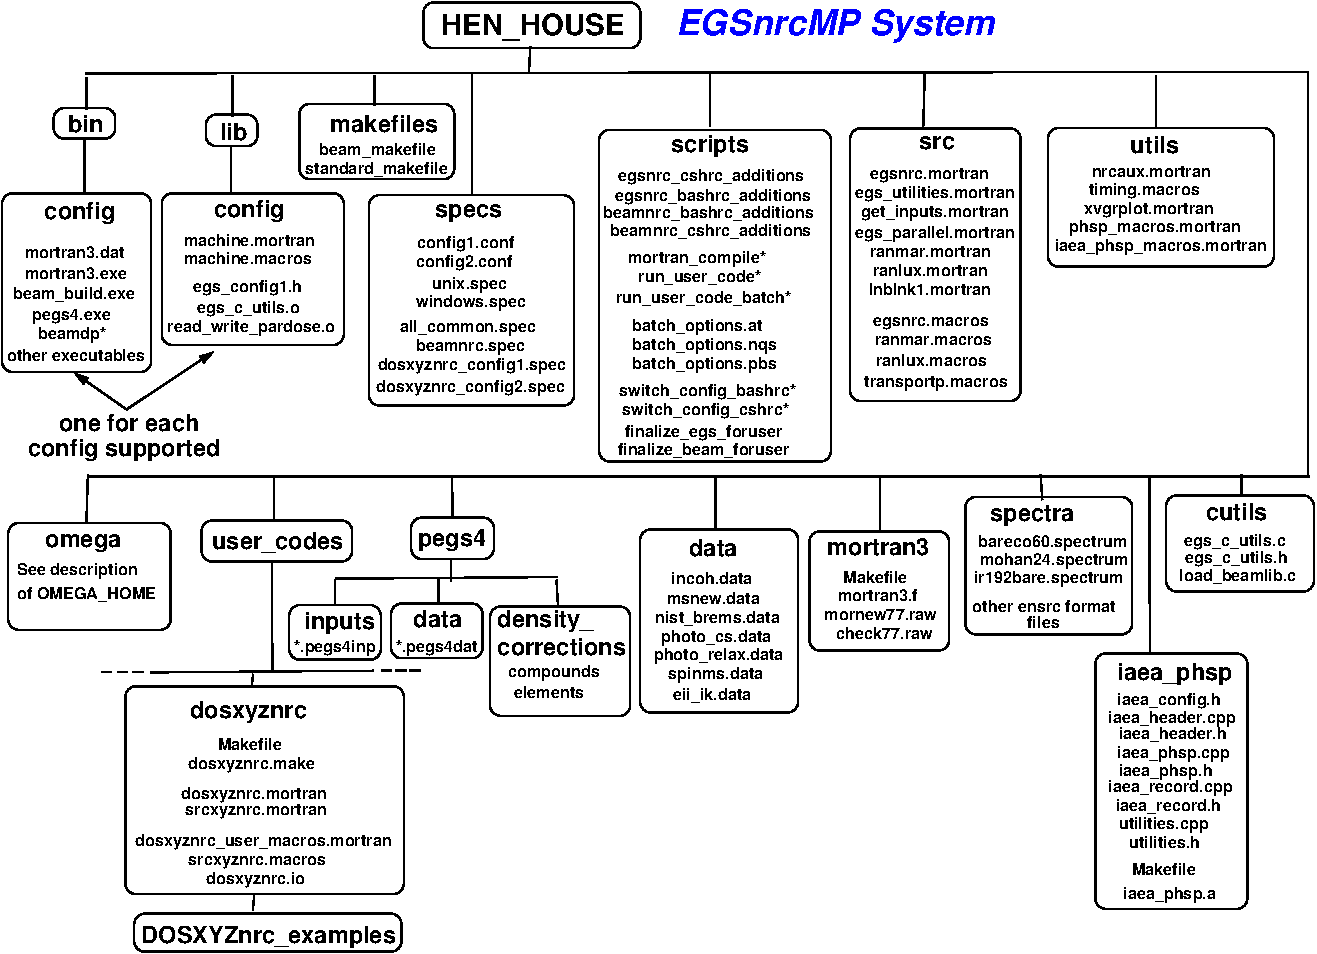
\includegraphics[width=15cm]{figures/egsnrc_system}
    \caption[Components of the {\tt HEN\_HOUSE} area for the EGSnrc
system.]
{The components of the {\tt HEN\_HOUSE} area for the EGSnrc
system. There are also subdirectories related to documentation and
NRC user codes which are not shown here and the main {\tt HEN\_HOUSE} box
actually has multiple subdirectories which are not shown. See PIRS-877 for
details\cite{Ka03}.}
\label{fig_hen_house_2}
\end{center}
\end{figure}

\clearpage

%\index{\$EGS\_HOME}
%\index{EGS\_HOME}
The second major  directory area of the EGSnrc system is
on the individual user's area and holds all the user's user codes and run associated
files.
It is mandatory that you set up a subdirectory which is referred to as
\verb+$EGS_HOME+ (e.g.,  frequently \verb+$HOME/egsnrc+) and for
each \verb+user_code.mortran+ which you use or write, there must be a sub-directory with
the same name as the user code, \ie~ \verb+$EGS_HOME/user_code+.
A typical user's area is shown in figure~\ref{fig_nrc_users_area}.
\begin{figure}[htb]
%\htmlimage{scale=1.6}   %this makes it readable
%\index{\$EGS\_HOME}
%\index{EGS\_HOME}
\index{EGSnrc!users area}
\index{user's area}
\begin{center}
\index{NRC EGSnrc user's area}
\index{user's area}
\leavevmode
\mbox{}\hspace{-1cm}
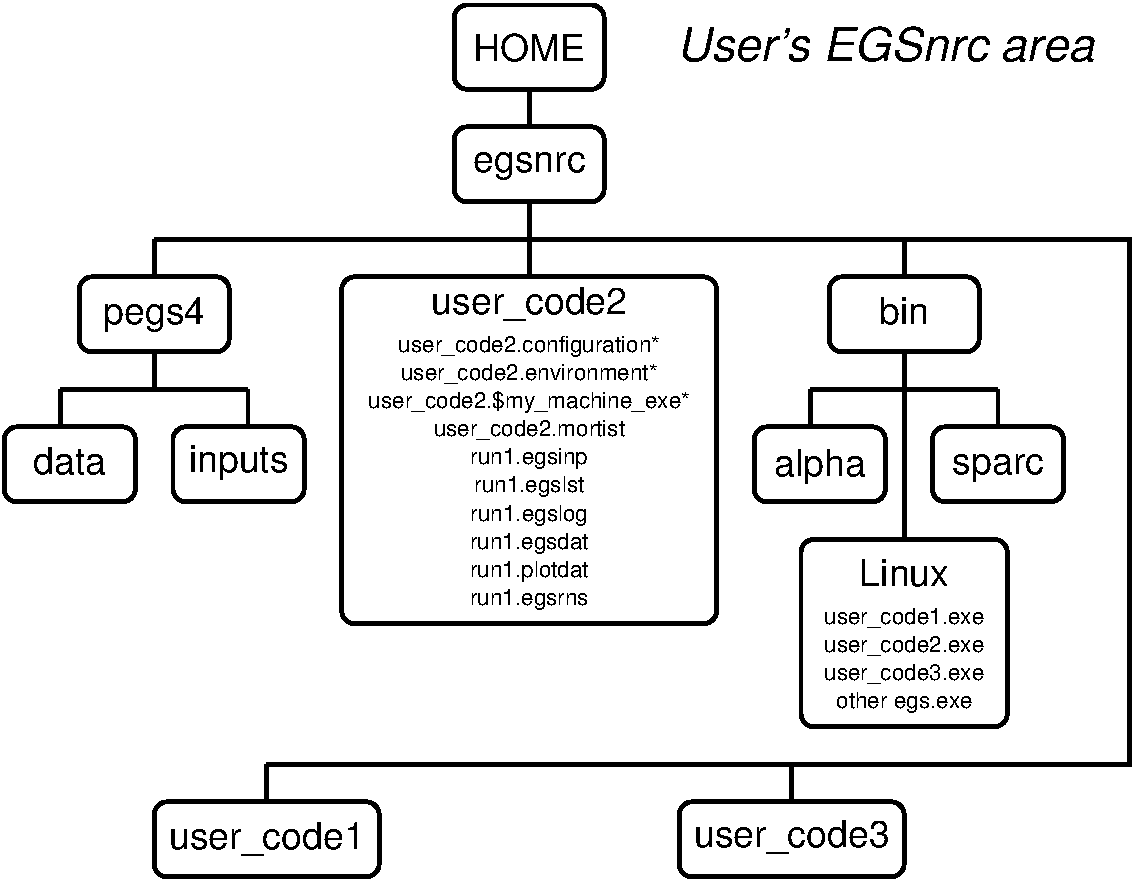
\includegraphics[width=14cm]{figures/users_egsnrc_area}
 \caption{Components of a typical EGS user's area where, for this
 example, {\tt \$EGS\_HOME} is {\tt \$HOME/egsnrc}. On a given system
 there can be an arbitrary number of different user's areas.
 \label{fig_nrc_users_area}
 }
\end{center}
\end{figure}

\subsubsection{A complication for multi-architecture systems}
\index{multi-architecture system}
% At NRC we run with a variety of different machines, all of which access
% a single disk system.  The EGSnrc system is set up to handle this
% transparently but this adds an additional level of complexity to the
% underlying system.  The system keeps track of which machine you are on
% at all times and uses the appropriate execute modules \etc.  This aspect
% of things is handled by the variable \verb+my_machine+ which essentially
% identifies the type of cpu currently being used and is determined by the
% script \verb+$HEN_HOUSE/get_machine+. The system is set up to store the
% executable files (the {\tt .exe}  files) on separate disk areas for each
% type of machine. To execute the code on different machine you must first
% compile it on each type of machine you want to use.  As new machines come
% along, the script \verb+$HEN_HOUSE/get_machine+ may become out of date and
% users may have to update it to return appropriate information for their
% system and more importantly, adjust the run and compile scripts to use the
% appropriate switches for their machine.
% \index{my\_machine}
% \index{get\_machine}
The install scripts are clever enough to establish various machine or
compiler dependencies and create the files {\tt
\$HEN\_HOUSE/lib/{my\_config}/machine.macros} and\\
 {\tt \$HEN\_HOUSE/lib/{my\_config}/machine.mortran} where {\tt
{my\_config}} is the name of your particular configuration (eg, g77,
gfortran, Mac).

\subsubsection{System aliases and environment variables}
\index{aliases} \index{environment variables}
\index{Cshrc\_additions\_for\_egsnrc}
\index{.login} \index{.cshrc}
\index{shell to use}
The EGSnrc system is based on using {\tt csh} C-shell scripts or {\tt sh},
bash shell scripts and to
facilitate this one should run from the C-shell ({\tt csh} or {\tt tcsh})
or the bash shell {\tt sh}.
To define the
aliases and other variables needed by the system, there are files called
{\tt egsnrc\_cshrc\_additions} and {\tt egsnrc\_bashrc\_additions} available on
{\tt \$HEN\_HOUSE/scripts}.
However, one first needs to set the environment variable {\tt HEN\_HOUSE}
to point at the location of the {\tt HEN\_HOUSE}. This is most conveniently
done with a declaration in your {\tt .login} file or {\tt .cshrc} file or
{\tt .bashrc} file depending on which shell is your default.
\begin{verbatim}
      setenv HEN_HOUSE location_of_HEN_HOUSE (e.g. $HOME/HEN_HOUSE)
\end{verbatim}
or for {\tt .bashrc}
\begin{verbatim}
      HEN_HOUSE=/absolute_location_of_your_HEN_HOUSE/ (e.g. $HOME/HEN_HOUSE)
\end{verbatim}
Then it is {\bfseries essential} that in your {\tt .cshrc} or {\tt .bashrc}
file you source the
{\tt  egsnrc\_cshrc\_additions} or {\tt egsnrc\_bashrc\_additions} file, i.e. add the statement:
\begin{verbatim}
     source $HEN_HOUSE/scripts/egsnrc_cshrc_additions}
\end{verbatim}
or, for those using {\tt bash}:
\begin{verbatim}
     source $HEN_HOUSE/scripts/egsnrc_bashrc_additions}
or
     source /absolute_location_of_your_HEN_HOUSE/scripts/egsnrc_bashrc_additions}
\end{verbatim}

These additions file set up many aliases and other variables for you. These
are most easily seen by executing the commands {\tt alias}, {\tt set} and
{\tt setenv} although this will show you all of the systems definitions as
well.  We will explain the use of many of these definitions in the
remainder of this section but the most important of the aliases are:
\index{egsnrc\_cshrc\_additions}
\index{egsnrc\_bashrc\_additions}

\index{mf} \index{mor} \index{f} \index{f} \index{ex} \index{mfb}
\index{PEGS4} \index{examin} \index{Mortran3!mor mf m}
\begin{description}
\item[mor]	MORTRAN a stand alone code
\item[m]	MORTRAN a specified users code
\item[mf]	MORTRAN and Fortran compile and link a specified users code
\item[f]	Fortran compile and link a specified users code
\item[ex]	execute an egs user code
\item[exb]	execute an egs user code in batch mode
%\item[pegs4]	run pegs4 (see section~\ref{pegs4_sc})
%\item[examin]   examin a particular data set from pegs4
%above not inlcuded now.
\end{description}
The use of these is described below in detail but note that the command
{\tt make} is now the easiest way to mortran and fortran user codes as
described in PIRS-877\cite{Ka03}.

% This script no longer here
%% The script {\tt
%% show\_settings} (on {\tt \$HEN\_HOUSE}) gives a more or less complete list
%% of all aliases, variables and environment variable associated
%% with EGSnrc once {\tt Cshrc\_additons\_for\_egsnrc} has been sourced. For
%% more detail see section~\ref{settings} (page~\pageref{settings}).
%% \index{show\_settings} \index{settings}



\newpage
\subsection{PEGS4}
\index{PEGS4}
\label{pegs4_sc}

As described elsewhere in this report, PEGS4 is the program which
prepares much of the material dependent cross section data sets required
by EGSnrc to do the simulations (see section~\ref{pegs4} on
page~\pageref{pegs4}).  As discussed there, use of the {\tt egs\_gui}
greatly facilitates the use of the {\tt PEGS4} program.

\index{.pegs4dat}
\index{.pegs4inp}
\index{densities for PEGS4}
The user must have the directories {\tt \$EGS\_HOME/pegs4},
{\tt \$EGS\_HOME/pegs4/inputs} and {\tt \$EGS\_HOME/pegs4/data}.
A user's PEGS4 input file is on {\tt \$EGS\_HOME/pegs4/inputs}
and has the name \verb+my_data.pegs4inp+.  The PEGS4 program outputs the
data file for EGSnrc to
\verb+$EGS_HOME/pegs4/data/my_data.pegs4dat+.
The listing file from the PEGS4
run is found on \verb+$EGS_HOME/pegs4+ and is called \verb+my_data.pegslst+.
To invoke PEGS4 one enters:
\begin{verbatim}
pegs4.exe -i inputfile [-o ofile] [-a] [-d density] [-x crosssection] [-e HEN_HOUSE]

inputfile.pegs4inp   the input file
output defaults to $HEN_HOUSE/pegs4/data/inputfile.pegs4dat
                or, if ofile is given, to $HEN_HOUSE/pegs4/data/ofile.pegs4dat
[-a]            => append results to output file
[-d density]    => use density.density   for density effect
[-x crosssection] => use $HEN_HOUSE/pegs4/crosssection instead of
                                $HEN_HOUSE/pegs4/pgs4pepr.dat
[-e HEN_HOUSE]  => use this absolute location as the HEN_HOUSE
\end{verbatim}
where \verb+my_data.pegsinp+ is the input file described in detail in
section~\ref{pegs4_input} (page~\pageref{pegs4_input}) and
\verb+density.density+
is a file containing the density effect information needed for this
particular calculation IF it is needed by \verb+my_data.pegsinp+.
The PEGS4 script checks the following directories, in order, for
the file \verb+density.density+.
\begin{verbatim}
$EGS_HOME/pegs4/inputs
$EGS_HOME/pegs4/density_corrections/elements
$EGS_HOME/pegs4/density_corrections/compounds
$EGS_HOME/pegs4/density_corrections
$HEN_HOUSE/pegs4/density_corrections/elements
$HEN_HOUSE/pegs4/density_corrections/compounds
\end{verbatim}

\subsubsection{Where pegs4 data is kept}
\index{PEGS4!where data is kept}
\index{.pegs4dat}
\label{wpdk}

Note that PEGS4 can only create one material output file per run and
if the simulation you want to run requires data for more than one material,
these must be joined into one \verb+file.pegs4dat+ file, either by
concatenation, by using an editor or by the {\tt -a} option in the command
line.

The EGSnrc run scripts look for the data file requested (see
section~\ref{Execution}), first on\\
\verb+$EGS_HOME/pegs4/data+ and if not
found there, then it looks on \verb+$HEN_HOUSE/pegs4/data+.
\vfill

\subsubsection{examin}
\index{EXAMIN}
The command:\\
\verb+examin -p file+
\\(note there is no ``e'' at the end of \verb+examin+) will allow you
to plot and/or list much of the photon and electron cross section data
in the file \verb+$EGS_HOME/pegs4/data/file.pegs4dat+ or if that is not
present, then in the file \verb+$HEN_HOUSE/pegs4/data/file.pegs4dat+. Note that
\verb+examin+ no longer displays the photon cross section data from the
PEGS4 data file but displays the data actually used by EGSnrc. The default
dataset used by \verb+examin+ is xcom. If you are using something else in your
user code, you must change the following line in the code:

\verb+REPLACE {$XDATA-DEFAULT} WITH {'xcom'}+

The output is found on \verb+$EGS_HOME/examin+. If requested, during execution
\verb+examin+ pops open \verb+xmgrace+ (a 2-D graphing package), otherwise
you have to use the listing files created. See section~\ref{examin}
(page ~\pageref{examin}).
\index{xmgrace}

\subsection{Compilation (MORTRAN and Fortran)}
\index{compiling}
\label{Compilation}

\index{Mortran3}

The EGSnrc system is written in the Mortran3 language which is
a pre-processor for Fortran.  Mortran3 is itself written in
Fortran.  The Mortran3 processor is part of the EGSnrc
distribution and is discussed in detail in section~\ref{UGM3},
page~\pageref{UGM3} of this report.  In order to create an executable file
from the mortran source files, there are two steps needed. The first step,
converts the mortran source code into standard Fortran77. We call this {\tt
MORTRAN} compiling.  The next step turns the Fortran source into an
executable, using the standard Fortran compile and link process.

Using the EGSnrcMP system (see PIRS-877\cite{Ka03}), the most direct way to
do these steps is using the {\tt make} command.  The following are the old
way to do it but they still work.

To ``compile'' the user code {\tt user\_code.mortran}, one issues the command:\\
\index{mf}\index{m}
\verb+mf user_code a [opt0|opt1|opt2|opt3|opt4]+\\
or\\
\verb+m user_code+\\

\index{Mortran3}
\index{Fortran}
The \verb+mf+ command will MORTRAN, Fortran and link the
entire user-code called \verb+user_code+, including the EGSnrc
system.  The Fortran and the execute modules are machine specific (SUN vs
SGI vs Linux etc) but this is handled in a transparent manner by the scripts.

The \verb+m+ command will MORTRAN the entire user-code
called \verb+user_code+, including the EGSnrc system. The output is
a Fortran file \verb+user_code_{my_machine}.f+ which is specific for the
machine being used since the script picks up a set of macros which
handles any differences between the machines.

The \verb+f+ command will Fortran and link the entire
Fortran version of the user-code called
\verb+user_code_{my_machine}.f+, which includes the EGSnrc system.
The scripts automatically detect the value for \verb+my_machine+ and use
the appropriate value.

\verb+user_code.mortran+ or \verb+user_code_{my_machine}.f+
must be present on area \\
\verb+$EGS_HOME/user_code+.

\index{compiling!options}
The letter {\tt a} after the user code name is a residual option which no
longer exists, but which has been left for compatibility with
a wide range of other scripts at NRC.  This option was associated with a
technique to avoid recompiling unchanged Fortran subroutines from one pass
to the next, but this was removed since compilers have become so fast that
it was not very useful and occasionally led to problems and always left
many extra files around. Note that  the
standard \verb+make+ facility does not work because the date on the Fortran
file is
always more recent than that on the object module since MORTRAN creates
a new version of the Fortran each time.


The option \verb+[opt0|opt1|opt2|opt3|opt4|debug]+ allows selection of
the optimisation level to be used.  For production codes, be sure to use
at least \verb+opt2+ since these can save up to 50\% over
\verb+opt0+, but they usually take much longer to compile and link.

\subsubsection{The  user\_code.configuration file (obsolete)}
\index{configuration file}
\index{.configuration file}
This approach has been completely revised and replaced by the {\tt
user\_code.make} file with {\tt SOURCES = } formats. See
PIRS-877\cite{Ka03}.  The same general capabilities have been maintained
in the new format.

During the MORTRAN stage, the scripts still create a file, called
\verb+.mortjob.mortran+ on \\
\verb+$EGS_HOME/user_code+. This file
contains all the source code for this
particular user\_code (macros, user\_code, and
any other routines the user wants, etc).
The files which are concatenated together to
form \verb+.mortjob.mortran+ are defined by the user.
% in the file\\
% \verb+$EGS_HOME/user_code/user_code.configuration+.  If this file is
% not present, the script uses the generic
% \verb+$HEN_HOUSE/standard.configuration+.  Figure~\ref{std_config} presents
% a listing of this file.
% \begin{latexonly}
% \input{standard.configuration}
% \end{latexonly}
% \begin{htmlonly}
% \clearpage
% \input{standard.configuration_html}
% \clearpage
% \end{htmlonly}



The {\tt .configuration} file (or new equivalent {\tt .make} file) allows for
very flexible options when compiling a given user
code.  For example, it is possible to change which random number generator
is being used throughout the system by merely changing which pair of files
are included in the configuration file, either {\tt ranlux.macros} and {\tt
ranlux.mortran} or {\tt ranmar.macros} and {\tt ranmar.mortran} (see
section~\ref{rngs}, page~\pageref{rngs}). However if
anything other than the default seeds and luxury levels are desired, there
may be some minor changes needed n {\tt user\_code.mortran}
unless one is very careful (\eg\ DOSRZnrc is designed to use either rng).
\index{RANMAR} \index{RANLUX}

\subsubsection{Order is Important}

The following still applies. When the file {\tt .mortjob.mortran} is
created, the order in which the various files are placed in the file is
important.  This is primarily because in Mortran3 the last definition of
any macro is the one that is in force.  Thus it is important that the {\tt
egsnrc.macros} file be read in early since this defines all of the default
values of the macros.  As long as it appears before the user code, then any
macro redefinitions done in the user code take precedence.

% the following no longer works so I removed the section
% \subsubsection{Batch compilations}
% \index{compiling!in batch}
% \index{batch!compiling}
% \index{batch}
% To compile in batch, just add a \verb+b+ to the above commands,
% \ie~\verb+mfb+ \etc. This will submit the compilation to whatever batch
% system you are using (see section~\ref{batch_que}).

\subsubsection{{\tt machine.mortran} files}
\index{machine.mortran}
Different compilers often have slightly different ways of handling certain
things.  The most common differences are regarding how files are opened
(i.e., the format of the {\tt OPEN} statement), and what is more difficult,
how they handle time.  EGSnrc itself has very few of these constructs
within it, but the user codes cannot avoid them.  To overcome these
differences, there are a series of macros defined in {\tt machine.mortran}
files which are found on {\tt
\$HEN\_HOUSE/lib/\$my\_machine/machine.mortran}.  It is even more complex
for Linux machines where the {\tt machine.mortran} files differ depending
on what version of the compiler you are using.  The default settings are
for a fairly recent {\tt g77} compiler but if you are using a slightly
older one you may need to edit the {\tt egs\_compile} script to select a
different default for the variable {\tt Linux\_compiler}.
\index{Linux\_compiler}

The {\tt  machine.mortran} files define a macro {\tt \$MACHINE} which the
user codes pick up. It is useful to define this properly in the {\tt
machine.mortran} which is picked up in your local environment.
\index{machine.mortran}
\index{\$MACHINE}

The above requirements are handled by a {\tt machine.mortran} which is
created for your system by the EGSnrcMP system as described in PIRS-877.


% no longer relevant so removed
% \subsubsection{{\tt get\_machine}, what if it fails?}
% \index{{get\_machine}}
% The script {\tt get\_machine} is designed to tell the EGSnrc scripts what
% type of machine is being used.  If the system you are using is not
% recognised by the scripts, it will try to compile using pretty vanilla
% flavoured compiler and loader flags.  The script will print out what flags
% it is using.  If you wish to change these to match the requirements of your
% machine, edit the {\tt egs\_compile} script. You may want to hard wire the
% selection of {\tt my\_flags} and {\tt my\_libs} to match your own
% machine/compiler.  If it is a common, new machine or compiler, please
% let us know what
% settings were needed and we will try to fit them into the next release.  We
% also hope to clean up these scripts and allow a more direct method to
% modify/tailor the system.
%



\subsection{Execution}
\index{execution}
\label{Execution}
\index{.egsinp}

The following works mostly still,, but there are new ways described in
PIRS-877\cite{Ka03} for the EGSnrcMP system.


Once a user code has been compiled, it is executed by issuing:

\hspace*{1cm}\verb+ex[b] user_code input data [queue|debug]+\vspace*{5mm}\\
\verb+$EGS_HOME/user_code/input.egsinp+ and\\
\verb+$EGS_HOME/user_code/user_code.{my_machine}_exe+ must exist.  The
PEGS4 data is in \verb+data.pegs4dat+ \index{.pegs4dat}which is located either on
the users area or the system area, as discussed in section~\ref{wpdk}.

\index{execution in batch}
If \verb+queue+ is not specified when the batch option ``{\tt b}'' is being
used, then the default queue on your system is used.
\index{interactive execution}

\index{debug}
In interactive mode, the 4-th input can be \verb+debug+ if a debug run
is wanted.  There must be an execute module created with the debug
switch set during compilation for this to work.

Execution of EGSnrc jobs is handled by the script {\tt egs\_run}
which is on the {\tt HEN\_HOUSE}.

At the completion of the run, all output and batch output files are
found on\\
\verb+$EGS_HOME/user_code/+ unless the user has specified something
different in the environment file (see below).

\index{execution!subdirectory during}
\index{subdirectory  during execution}
During execution, the {\tt egs\_run} script creates a separate subdirectory area
and only modifies the files there. This is usually a subdirectory of
\verb+$EGS_HOME/user_code/+ but on a Linux system is on {\tt /tmp}
(this is to
make the subdirectory local to the machine running the job since on the NRC
system, having the disk on another machine would seriously slow down the
job). All
the files are moved back to \verb+$EGS_HOME/user_code/+ after
completion of the run.  This can be confusing unless you are aware of this
behaviour.

\subsubsection{user\_code.environment file (obsolete)}
\index{.environment file}
\index{environment file}

This functionality is reworked and described in PIRS-877\cite{Ka03}.  In
particular the {\tt user\_code.io} file is relevant although the general
ideas below are still applicable.

% The execution scripts source
% \verb+$EGS_HOME/user_code/user_code.environment+ immediately prior to
% executing the \verb+user_code+ and then again immediately after.  An
% example  is given in
% \verb+$HEN_HOUSE/example_usercode.environment+ which is shown in
% figure~\ref{ex_environment}.  In general, this file defines the links to
% specific files from Fortran units, \etc.
%
Almost all Fortran compilers associate a file called {\tt fort.n} with any I/O
unit {\tt n} which is not attached explicitly within the code to some
file name. Thus if {\tt HATCH} read data from unit 12 without any open
statement, then it looks for {\tt fort.12}.  The system must associate
this file name to the real file name.
There are a series of similar links established
for files which have common names for all user codes.

% \begin{latexonly}
% \input{example_usercode.environment}
% \end{latexonly}
% \begin{htmlonly}
% \clearpage
% \input{example_usercode.environment_html}
% \clearpage
% \end{htmlonly}




The following files are associated with a normal type of run with an NRC
user code (although the environment files can add whatever files the user
may want and the files below are not mandatory).  For
this example, the input file name is \verb+input.egsinp+.
\begin{description}
\item [input.egsinp:] defined by the user.
\item [input.egslst:]  the output listing file from the run. Erased
at start of next run if not renamed.
\item [input.egslog:] The log file which echos the inputs and
prompts when running in batch. Note, this has most of the {\bf error}
messages too, so get in the habit of reading this file.
\item [input.egsdat:] A file containing all the information needed to
allow a calculation to be resumed.
\item [input.egsrns:] Some codes allow a record of random number seeds
at the start of each history to be kept (just most recent). These are
kept in this file if requested.
\item [input.egsplot (etc):] Plotting files for various routines, the
most up to date are for \verb+xmgrace+.
\index{xmgrace}
\item [input.egsgeom:] file with output description of geometry for
\verb+EGS_windows+.
\item [input.egsgph:] file with output phase space of each history for
\verb+EGS_windows+.
\end{description}

% The one known exception to the rule above about {\tt fort.n} files names is the
% HP unix system.  Here the default Fortran unit name is {\tt ftn05} for {\tt
% fort.5} etc. The approach here is to use statements like {\tt setenv ftn11
% fort.11} in the {\tt .environment} file prior to the link statement. This
% is done within {\tt egs\_run} for  many units which are regularly used.

\subsubsection{Batch Queues (obsolete)}
\label{batch_que}
See PIRS-877 for how this is handled now.


\subsection{Parallel Processing}
\label{pprocess}
\index{pprocess}
\index{parallel processing}
\index{NQS}

The following is replaced by a more sophisticated approach in the EGSnrcMP
system and the standard NRC user codes. See PIRS-877\cite{Ka03}.

Monte Carlo calculations with EGSnrc are easily run in parallel and the
results combined at the end of the runs because every history is completely
independent, as long as the random number sequences are independent. One of
the reasons for selecting the random number generators distributed with
EGSnrc is that there is a simple procedure for ensuring independent
sequences (see section~\ref{rngs} on page~\pageref{rngs}).

The NRC user codes\cite{Ro00} have a parallel processing option built in.
The system used requires the NQS batch submission system to be installed on
all machines to be run in parallel. The option is implemented via a script,
called {\tt pprocess} which makes an arbitrary number of input files from
the original file, ensuring different random number sequences for each and
then submitting the job to an arbitrary number of machines.  At the end of
the runs, the main user code is run once more with instructions to combine
the results of the previous runs.  Although crude, it is highly effective.
We routinely run using more than 30 of our 38 CPUs running in parallel.
The script {\tt combine\_egsnrc} has been written to automatically edit the
required input file and execute the needed final run for the analysis of
parallel runs with the NRC user codes.
There is more discussion in reference~\cite{Ro00}.
\index{combine\_egsnrc}

Note that there is a useful script called {\tt
clean\_after\_parallel} which is found on\newline {\tt \$HEN\_HOUSE/scripts}.
Parallel runs create a huge number of files and this script helps clean
them up, but only once they have been analysed.
\index{clean\_after\_parallel}


\subsection{Distribution / Installation of EGSnrc}
\label{install}
\index{distribution}
\index{installation}
\index{Cshrc\_additions\_for\_egsnrc}
\index{INSTALL\_EGS}


\index{.cshrc}
\index{HEN\_HOUSE}
This installation script requires that the environment variables
\verb+HEN_HOUSE+ not be defined when the script is called and not be
defined in the user's {\tt .cshrc} or {\tt .bashrc} file. The installation will create
the entire \verb+$HEN_HOUSE+ structure shown in
fig~\ref{fig_hen_house_2} (page~\pageref{fig_hen_house_2})
and compile a variety of codes for the machine
the user is doing the installation from (\viz\ Mortran3,
PEGS4, DOSRZnrc).  It also partially sets up the user's area
\verb+$EGS_HOME+.

Once the \verb+INSTALL_EGS+ script has been successfully executed, one
must ensure that the environment variables {\tt HEN\_HOUSE} and {\tt
EGS\_HOME} are defined to
point at wherever you have placed the EGSnrc system and your EGSnrc user
area.

Most importantly, the installation leaves behind a file called
\verb+egsnrc_cshrc_additions+ or \verb+egsnrc_bashrc_additions+
which MUST be sourced from the user's
{\tt .cshrc} script or {\tt .bashrc} script depending on which default
shell is used. Once the installation is complete,
add the following to your {\tt .cshrc} file:\\
\verb+source /explicit_path_to_your_HEN_HOUSE/egsnrc_cshrc_additions+. \\
or the following to your {\tt .bashrc} file:\\
\verb+source /explicit_path_to_your_HEN_HOUSE/egsnrc_bashrc_additions+. \\
\index{egsnrc\_bashrc\_additions}
\index{egsnrc\_cshrc\_additions}

The user should try to run the {\tt tutor} codes to ensure the system is working.

% For examples of the files created by {\tt INSTALL\_EGS}, see\\
% {\tt \$HEN\_HOUSE/test\_distribution\_outputs}.
% \index{example lst\_install files}
%
% One can also run the script {\tt test\_distribution} (see
% section~\ref{test_distribution}, page~\pageref{test_distribution}) which
% exercises the system extensively.
% \index{test\_distribution}.


% \subsection{On-Line Manuals}
% \index{on-line manuals}
% The manuals for the EGSnrc system are on-line from the same site as the
% distribution.
% \subsection{Changes and bugs corrected since initial release}
% \label{fixed_bugs}
% \index{bugs}
% \index{corrected bugs}
%
% %%%%%%%%%%%%%%%%%%%%%%%%%%%%%%%%%%%%%%%%%%%%%%%%%%%%%%%%%%%%%%%%%%%%%%%%%%%
% \noindent The following changes were made to EGSnrc in a minor release in Oct, 2001
% %%%%%%%%%%%%%%%%%%%%%%%%%%%%%%%%%%%%%%%%%%%%%%%%%%%%%%%%%%%%%%%%%%%%%%%%%%%
% \begin{itemize}
% \item A call to AUSGAB immediately prior to annihilation of a positron at
% rest was added with IARG=28.
%
% \item The auxiliary input routine for EGSnrc parameters was changed to use
% macros to define the defaults.
%
% \item A change was made to allow {\tt skindepth\_for\_bca} to be less than
% 1.
% \item James Tickner pointed out that K-alpha1 and K-alpha2 transition
% probabilities had been inverted.  This was fixed.
%
% \end{itemize}
%
% \noindent The following changes were made to EGSnrc in the May, 2001 release.
% \begin{itemize}
% \item WT = 0.0 now causes new particles to be discarded immediately via the
% \\
% {\tt USER-PHOTON-DISCARD} and {\tt USER-ELECTRON-DISCARD} exits which
% generate {\tt IARG = 3} exits.  This saves time and avoids other problems
% (see section~\ref{termination}, page~\pageref{termination}).
% \item {\tt \$COMIN-RELAX} is now defined in {\tt egsnrc.macros} instead of
% in {\tt subroutine relax}.
% \end{itemize}
%
% %%%%%%%%%%%%%%%%%%%%%%%%%%%%%%%%%%%%%%%%%%%%%%%%%%%%%%%%%%%%%%%%%%%%%%%%%%%
% \noindent The following bugs in EGSnrc were fixed in the May, 2002 release.
% %%%%%%%%%%%%%%%%%%%%%%%%%%%%%%%%%%%%%%%%%%%%%%%%%%%%%%%%%%%%%%%%%%%%%%%%%%%
%
% \begin{itemize}
% \item If using the SLAC geometry macros, the COMIN's did not contain the
% needed declarations of the variables.
% \item Daniel Frei from Bern pointed out an error which affected a charged
% particle going directly backwards along the Z axis.
% \item Format of the region number output by {\tt subroutine WATCH} was
% changed so that it would work for region numbers greater than 9,999. The
% original format caused {\tt EGS\_Windows} to misbehave.
% \item Alex Bielajew pointed out that egs\_batch does not work when using the
% standard at batch command due to extra white space.
% \item Permissions on data sets are changed to allow world read access.
% \item Omar Chibani pointed out that the density scaling didn't work
% properly. This has been fixed and the manual also made clearer.
% \item History by history statistical analysis was implemented in all user
% codes.
% \end{itemize}
%
% %%%%%%%%%%%%%%%%%%%%%%%%%%%%%%%%%%%%%%%%%%%%%%%%%%%%%%%%%%%%%%%%%%%%%%%%%%%
% \noindent The following bugs in EGSnrc were fixed in the Nov., 2003 release.
% %%%%%%%%%%%%%%%%%%%%%%%%%%%%%%%%%%%%%%%%%%%%%%%%%%%%%%%%%%%%%%%%%%%%%%%%%%%
%
%
% \begin{itemize}
% \item Many improvements to the GUI's and the entire new EGSnrcMP
% environment (see Report PIRS-877\cite{Ka03} for an extensive discussion).
%
% \item Fixed the ranlux RNG so that restarting a specific history is now
% possible (useful for debugging purposes).
%
% \item Fixed a bug pointed out by Rebecca Nutbrown re normalization of
% results when a phase-space source was recycled.
%
% \item Fixed a bug in FLURZnrc.mortran regarding electron fluence in bins
% below ECUT.
%
% \item Fixed a serious normalization bug in DOSRZnrc for the case where
% parallel runs were done using a phase-space source. The bug was pointed
% out by Roberto Capote who also pointed out a similar sort of bug which
% applied to all the RZ codes when using a phase space source and recycling
% the source.
%
% \item Bug in the {\tt preview3d} code for use with EGS\_Windows for
% cylindrical geometries was fixed.
%
% \item A bug, which was pointed out by Wamied Abdel-Rahman and Frank Verhaegen
% regarding positron annihilation when using the NIST cross sections for
% bremsstrahlung	production, was fixed.
%
% \item A bug related to discards for being below ECUT and PCUT in a vacuum
% was fixed.
% \end{itemize}
%
%
%
% \subsection{Known bugs/restrictions}
% \index{Known bugs}
% \index{restrictions}
%
% Straggling in the continuous energy loss is not modelled.
%






\clearpage
%%%%%%%%%%%%%%%%%%%%%%%%%%%%%%%%%%%%%%%%%%%%%%%%%%%%%%%%%%%%%%%%%%%%%%%%
\typeout{}
\typeout{***Start of Cited References****}
\typeout{}
%%%%%%%%%%%%%%%%%%%%%%%%%%%%%%%%%%%%%%%%%%%%%%%%%%%%%%%%%%%%%%%%%%%%%%%%
\renewcommand{\leftmark}{{References}}
\renewcommand{\rightmark}{{References}}

\section*{References}
\addcontentsline{toc}{section}{\numberline{}References}
\vspace*{-1.7cm}
\bibliography{../irs}
\typeout{}
\typeout{******REMEMBER to create .bbl  and reset twice**********}
\typeout{}
\bibliographystyle{unsrt}



\newpage
\typeout{**********starting index here******************}
\renewcommand{\leftmark}{{Index}}
\renewcommand{\rightmark}{{Index}}
\addcontentsline{toc}{section}{\numberline{}Index}
\setlength{\baselineskip}{0.5cm}


%%%%%%%%%%%%%%%%%%%%%%%%%%%%%%%%%%%%%%%%%%%%%%%%%%%%%%%%%%%%%%%%%%%%%%%%%%%%%%%
%
%  EGSnrc manual
%  Copyright (C) 2015 National Research Council Canada
%
%  This file is part of EGSnrc.
%
%  EGSnrc is free software: you can redistribute it and/or modify it under
%  the terms of the GNU Affero General Public License as published by the
%  Free Software Foundation, either version 3 of the License, or (at your
%  option) any later version.
%
%  EGSnrc is distributed in the hope that it will be useful, but WITHOUT ANY
%  WARRANTY; without even the implied warranty of MERCHANTABILITY or FITNESS
%  FOR A PARTICULAR PURPOSE.  See the GNU Affero General Public License for
%  more details.
%
%  You should have received a copy of the GNU Affero General Public License
%  along with EGSnrc. If not, see <http://www.gnu.org/licenses/>.
%
%%%%%%%%%%%%%%%%%%%%%%%%%%%%%%%%%%%%%%%%%%%%%%%%%%%%%%%%%%%%%%%%%%%%%%%%%%%%%%%
%
%  Authors:         Iwan Kawrakow
%                   Ernesto Mainegra-Hing
%                   Dave Rogers
%                   Frederic Tessier
%                   Blake Walters
%
%  Contributors:
%
%%%%%%%%%%%%%%%%%%%%%%%%%%%%%%%%%%%%%%%%%%%%%%%%%%%%%%%%%%%%%%%%%%%%%%%%%%%%%%%


\documentclass[12pt,twoside]{article}  %indexm doesn't work with two sides
%\usepackage{supertab}%this didn't work for some reason?

\usepackage{moreverb}	%this is used for the boxedverbatim environment
			%used to box the listing files for tutor programs
\usepackage{amsmath}
%\usepackage{showidx}    %shows index entries

\setlength{\textwidth}{16.51cm}
%\setlength{\textheight}{23.2cm}
\setlength{\textheight}{23.5cm}
\setlength{\oddsidemargin}{0.0in}
\setlength{\evensidemargin}{0.0in}
\setlength{\topmargin}{-1.5cm}
\setlength{\parindent}{1.5em}
\setlength{\topsep}{0ex}
\setlength{\itemsep}{0ex}

\newcommand{\Mol}{Moli\`ere}

\newcommand{\Co}{$^{60}$Co}
\newcommand{\parsp}{~\hspace*{1.5em}}
\setlength{\parskip}{0.1in}
\setlength{\baselineskip}{1.0cm}
\newcommand{\head}[1]{\begin{center}\begin{Large}{\bf #1}
                                              \end{Large}\end{center}}
\newcommand{\cen}[1]{\begin{center} #1 \end{center} }
\newcommand{\etal}{{\em et.al.}}
\newcommand{\ie}{{\em i.e.}}
\newcommand{\etc}{{\em etc.}}
\newcommand{\viz}{{\em viz.}}
\newcommand{\eg}{{\em eg.}}
\newcommand{\note}[1]{\mbox{}\\ \noindent \rule{16cm}{0.5mm} \\
{\em #1} \\ \noindent \rule{16cm}{0.5mm}\\
\typeout{***********note active on this page *************************}
}

%\newcommand{\indexm}[1]{\index{#1}}
%\typeout{~~~~~~~~~~~~***margin index feature OFF*****************************}
%\typeout{~~~~~~~~~~~~***margin index feature OFF*****************************}
%\typeout{~~~~~~~~~~~~***margin index feature OFF*****************************}
\newcommand{\indexm}[1]{\marginpar{{\sf {\tiny I:#1} }}\index{#1}}
\makeindex

%	some commands to get 4 levels in the table of contents and
%	number down to paragraphs
\setcounter{secnumdepth}{4}
\setcounter{tocdepth}{4}
\renewcommand{\thesubsubsection}{\thesubsection.\arabic{subsubsection}}
\renewcommand{\theparagraph}{\thesubsubsection.\roman{paragraph}}
\renewcommand{\theequation}{\arabic{subsection}.\arabic{subsubsection}.\arabic{equation}}

\renewcommand{\theenumii}{\roman{enumii}}
\renewcommand{\labelenumii}{\theenumii.}

%\renewcommand\paragraph{\@startsection{paragraph}{4}{\z@}%
%                                    {3.25ex \@plus1ex \@minus.2ex}%
%                                    {-1em}%
%                                    {\normalfont\normalsize\bfseries}}
%above is copied from article.cls and it still causes a hang up!!
%above explained p25-26 Latex Companion

\renewcommand{\refname}{}


\usepackage[breaklinks]{hyperref}
\usepackage{epsf}
\usepackage{graphicx}
\usepackage{epsfig}
\usepackage{longtable}

%\input{epsf}

%\usepackage{fancyheadings}
\usepackage{fancyhdr}
\usepackage{html}
\renewcommand{\footrulewidth}{0.4pt}
\renewcommand{\headrulewidth}{0.4pt}

\lhead[{\sffamily \thepage}]{{\sffamily {EGSnrc} Code System }}
\rhead[{\sffamily NRCC Report PIRS-701 }]{{\sffamily ~\thepage}}
%\rfoot[{\sffamily {\rightmark}}]{{\sffamily {\rightmark}}}
\rfoot[]{{\sffamily {\rightmark}}}
% Replace line with fixed date with the one below when commiting
% Beware: Using the macro below conflicts between CVS and latex!!!
% \lfoot[{\sffamily {\leftmark}}]{{\small Last edited $Date: 2013/09/26 17:59:57 $
\lfoot[{\sffamily {\leftmark}}]{{\small Last edited 2011/05/02 18:36:27
}}
\cfoot{}

\begin{latexonly}
\typeout{***Have turned off overfull and underfull messages****}
\tolerance=10000        %suppress Overfull only
\hbadness=10000         %suppress Overfull and Underfull for text (horizontal)
\vbadness=10000
\end{latexonly}

\begin{document}

\begin{htmlonly}
For information about the authors and/or institutions involved with this
work, use the links provided in the author list.\\
\begin{rawhtml}
<br><br>
\end{rawhtml}


\begin{rawhtml}
<br><br>
\end{rawhtml}

Postscript and pdf versions of the entire report are available.  You may have to
download the compressed version to disk, uncompress or gunzip them and
then read or print them.\\
\begin{center}
\htmladdnormallink{(uncompressed version 2.2 Mbyte)}{pirs701.ps}\\
\htmladdnormallink{(gzip version 670 kbyte)}{pirs701.ps.gz}\\
\htmladdnormallink{(pdf version 1.2 Mbyte)}{pirs701.pdf}
\end{center}
\begin{rawhtml}
<br><br>
\end{rawhtml}

Use the Up button to get back to this page from within the document.
\begin{rawhtml}
<BR> <HR> <P>
\end{rawhtml}
\copyright
Copyright 2000 -- 2015, National Research Council of Canada
Ottawa
\begin{rawhtml}
<BR> <HR> <P>
\end{rawhtml}
\end{htmlonly}

\pagestyle{empty}
%%%%%%%%%%%%%%%%%%%%%%%%%%%%%%%%%%%%%%%%%%%%%%%%%%%%%%%%%%%%%%%%%%%%%%%%

%               Title page to  preface

%%%%%%%%%%%%%%%%%%%%%%%%%%%%%%%%%%%%%%%%%%%%%%%%%%%%%%%%%%%%%%%%%%%%%%%%

\title{EGSnrc Code System}

\begin{center}
{\sffamily \bfseries {\Huge The EGSnrc Code System:}\\
{\Large Monte Carlo Simulation of Electron and Photon Transport
\vspace{5mm}\\}}
\begin{large}
I. Kawrakow\\
E. Mainegra-Hing, D.W.O. Rogers, F. Tessier and B.R.B. Walters\\
\end{large}
Ionizing Radiation Standards,\\
National Research Council Canada,\\
Ottawa, Canada\\

\vspace{10mm}
{\bfseries
\today}
\vspace{5mm}\\
\hfill NRCC Report {\sf PIRS-701} \vspace*{15mm}\\


\begin{figure}[h]
\begin{center}
\htmlimage{scale=1.2}
\leavevmode
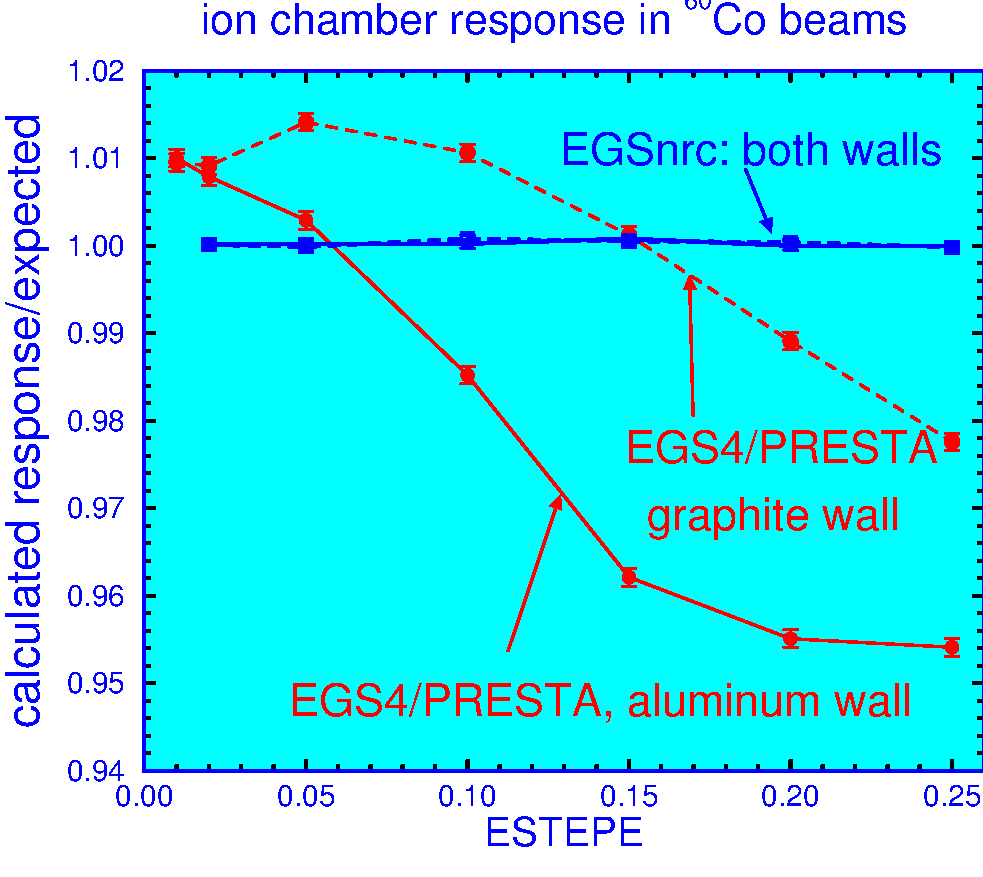
\includegraphics[height=10.5cm]{figures/ion_chamber}
%\caption{Improvement of EGSnrc compared to EGS4/PRESTA.}
%\cen{\Large Improvement of EGSnrc compared to EGS4/PRESTA.}
\end{center}
\end{figure}
\vfill

\copyright NRC Canada, 2001--2015
\end{center}
\newpage   %Blank page behind cover
\mbox{}


\newpage
\setlength{\baselineskip}{0.5cm}

\pagestyle{fancy}
\pagenumbering{arabic}
\setcounter{page}{1}


%%%%%%%%%%%%%%%%%%%%%%%%%%%%%%%%%%%%%%%%%%%%%%%%%%%%%%%%%%%%%%%%%%%%%%%%%%%%%%%
%
%  EGSnrc manual: preface
%  Copyright (C) 2015 National Research Council Canada
%
%  This file is part of EGSnrc.
%
%  EGSnrc is free software: you can redistribute it and/or modify it under
%  the terms of the GNU Affero General Public License as published by the
%  Free Software Foundation, either version 3 of the License, or (at your
%  option) any later version.
%
%  EGSnrc is distributed in the hope that it will be useful, but WITHOUT ANY
%  WARRANTY; without even the implied warranty of MERCHANTABILITY or FITNESS
%  FOR A PARTICULAR PURPOSE.  See the GNU Affero General Public License for
%  more details.
%
%  You should have received a copy of the GNU Affero General Public License
%  along with EGSnrc. If not, see <http://www.gnu.org/licenses/>.
%
%%%%%%%%%%%%%%%%%%%%%%%%%%%%%%%%%%%%%%%%%%%%%%%%%%%%%%%%%%%%%%%%%%%%%%%%%%%%%%%
%
%  Author:          Iwan Kawrakow, 2003
%
%  Contributors:    Blake Walters
%                   Frederic Tessier
%                   Ernesto Mainegra-Hing
%
%%%%%%%%%%%%%%%%%%%%%%%%%%%%%%%%%%%%%%%%%%%%%%%%%%%%%%%%%%%%%%%%%%%%%%%%%%%%%%%


\newpage
\mbox{ }\vspace*{-35mm}\\
\section*{\begin{center}Preface\end{center}}
\addcontentsline{toc}{section}{\numberline{}Preface}
\index{preface}
% Replace commented line for the one with fixed date when commiting
% Beware: Using the macro below conflicts between CVS and latex!!!
% \lfoot[{\sffamily {\leftmark}}]{{\small Last edited $Date: 2013/01/04 15:08:41 $
\lfoot[{\sffamily {\leftmark}}]{{\small Last edited 2011/05/02 18:36:27
}}
\mbox{ }\vspace*{-5mm}\\
\noindent {\bfseries Sixth printing: May 2011}\\
A long time has passed since the last update to this document.
Although no fundamental changes have been made to the system,
there have been a number of important additions and improvements
to the system since 2009. Numerous bugs have been corrected and
a new user code for free-air chamber (FAC) correction calculations
was added to the distribution.
\begin{itemize}
\item Use of arbitrary electron impact ionization (EII)
cross section compilations. Added a data base of EII
cross sections based on the DWBA/PWBA theory by
Bote and Salvat.
\item For backward compatibility with previous calculations, users can
now request the use of PEGS4 photon data.
\item Inclusion of C++ {\tt egs\_fac} application with example.
This user-code implements a self-consistent algorithm for the
fast calculation of FAC correction factors.
\item EII cross sections printout for materials in
  the simulation if user requests output of the photon cross-sections.
\item Updated several GUI's to include most of the latest additions
and corrected several bugs.
\end{itemize}
% \vspace{3mm}\\
\noindent {\bfseries Fifth printing: July 2009}\\
There has been a huge number of changes in the system since
the last printing in November 2003 that have not been properly
added to the documentation. This printing is an attempt to update
this report to better reflect the state of EGSnrc, although it
is far from complete. The development of the EGSnrc C++ class
library, which includes a general purpose geometry package, and its
first public release in 2005 has been a major step forward.
The C++ class library is described in a separate report (PIRS--898).
Major changes and additions to the EGSnrc physics include:
option to simulate electron impact ionization, an improved
bremsstrahlung data base that includes an exact evaluation of
electron-electron bremsstrahlung in the first Born approximation,
an improved differential pair production cross section tabulation
based on exact PWA calculations that takes into account the asymmetry
of the energy distribution at energies close to the threshold,
the ability to explicitely
simulate triplet interactions (\ie, pair production in the electron field),
the ability to take into account radiative corrections for Compton
scattering in the one-loop approximation, the ability to use
user-supplied atomic and molecular form factors for Rayleigh scattering,
and the ability to use total photon cross sections from EPDL97, XCOM, or
any other user-supplied tabulation in addition to the default
Storm \& Israel tabulations.
New options added for Compton scattering called {\tt simple} and
{\tt norej}. When using {\tt simple} binding is taken
into account via an incoherent scattering function
ignoring Doppler broadening. The incoherent scattering function
is still obtained from the impulse approximation.
The {\tt norej} option uses actual bound Compton cross section
when initializing the photon cross sections and rejections in
subroutine COMPT lead to re-sampling rather than rejecting the
entire interaction.
An {\tt alias sampling} algorithm is now used to select the
photon angle after a Rayleigh scattering to avoid an undersampling
at large angles observed in the original EGS4 implementation.
Particle track scoring object added to the {\tt egspp} library
allowing visualization of particle tracks with the C++ geometry
viewer {\tt egs\_view}. See example input file tracks1.egsinp for
the tutor7pp C++ user-code.

Finally, to better reflect their contributions
to the development and maintenence of the system, Ernesto Mainegra-Hing,
Blake Walters and Frederic Tessier have been added as co-authors.
\vspace{3mm}\\
\noindent {\bfseries Fourth printing: November 2003}\\
Added references to EGSnrcMP and Report PIRS-877. A few minor changes
related to the major change in the operating system to make it Windows
compliant. There is no associated change in the physics of the system.
Table 7 re timing of random numbers has changed substantially.
\vspace{3mm}\\
\noindent {\bfseries Third printing: April 2002}\\
Minor changes reflecting code changes.
%See section~\ref{fixed_bugs}.
\vspace{3mm}\\
\noindent {\bfseries Second printing: May 2001}\\
The second printing contains a description of the use of {\tt RHOF}
(section~\ref{RHOF_RHOR}, page~\pageref{RHOF_RHOR}) and {\tt \$SET-RHOF}
(section~\ref{set_rhof}, page~\pageref{set_rhof}). There is a brief new
discussion of {\tt combine\_egsnrc}, a script for automatic analysis of the
many files created by {\t pprocess} in parallel runs
((section~\ref{pprocess}, page~\pageref{pprocess})). There is a new section
about terminating histories with WT=0.0 (section~\ref{termination},
page~\pageref{termination}).
%Finally, a new section
%has been added which documents the few minor changes made to EGSnrc since
%its initial release ((section~\ref{fixed_bugs},
%page~\pageref{fixed_bugs})).
\vspace{3mm}\\
\noindent {\bfseries First printing: May 2000}\\
In the decade and a half since the original version of EGS4 was released
there have been well over 1000 papers published which cite the original
SLAC-265 Report.  The code itself has been improved in many different ways
by a large number of people.  For a detailed history of much of this up to
1994, the reader is referred to a report titled  ``History, overview and
recent improvements of EGS4'' by Bielajew et al.
\index{Bielajew, Alex}

In the last few years there have been significant advances in several
aspects of electron transport.  For example, improvements in multiple scattering
theory have been developed by Kawrakow and Bielajew\cite{KB97,Bi96,Ka96}
which get over most of
the shortcomings of the Moliere theory used in EGS4. Perhaps more important
has been the development by Kawrakow and Bielajew\cite{KB97a} of a new electron transport algorithm, sometimes
called PRESTA-II, which makes a significant advance in the science of
electron transport.  In addition to these advances, Kawrakow has implemented
several other improvements in the electron transport algorithm of EGS
which make it capable of accurately calculating ion chamber response at the
0.1\% level (relative to its own cross sections)\cite{Ka99a,Ka99b}.

EGSnrc also has implemented a variety of additional features, many of
which have previously been extensively developed as additions to EGS4
by  Namito, Hirayama and Ban at KEK as well\cite{Na98,Na95a,Na94,Na93}.
The EGSnrc approach differs from that of the KEK group, partially because
once we were making fundamental changes to the code, we carried it through
in a consistent manner. However, the KEK group have implemented several
options which are not yet in EGSnrc (e.g.  polarized photon scattering
and electron impact ionization).
\index{Hirayama, Hideo} \index{Namito} \index{Ban}

This report is meant to document the many changes that have occurred going
from EGS4 to EGSnrc.  Although this report is written by two people,
the EGS system is obviously the child of many parents who have made a
wide variety of contributions over the years.  This goes right back to
Richard Ford, then at SLAC, who was a major contributor to EGS3. Hideo
Hirayama, S Ban  and Yosh Namito of KEK have made innumerable contributions
to EGS, especially concerning the low energy photon physics. Alex
Bielajew worked on EGS at NRC from the early 80's to late 90's and his
name is linked to a huge number of important contributions to EGS,
perhaps most importantly the PRESTA algorithms, but also many other
specific improvements to the physics, the Unix based scripts and the NRC
user codes. His name appears very extensively in the reference lists.
The name of Walter Ralph Nelson is practically synonymous with EGS and
all users of any version of the EGS system will forever be in Ralph's
debt. It has been his enthusiasm and willingness to help others and share
this resource so selflessly which has made it the great success it is.
To all of these people who have contributed so extensively to the EGS
system, and to the countless others who have played a variety of roles,
we all owe a huge debt of gratitude.
\index{Nelson, Ralph}


It is worth noting that NRC and SLAC have drawn up a formal agreement which
recognizes that both have rights associated with EGS4 and EGSnrc.  Thus, in
this report there are sections which are taken verbatim from SLAC-265 (in
particular the PEGS4 manual and the User's guide to Mortran3) and we wish
to thank SLAC for permission to reproduce them.  We also draw attention to
the copyright and licensing arrangements associated with EGSnrc which are
similar to those for EGS4, but which are becoming more tightly controlled
in this changing world we live in.  Neither EGS4 nor EGSnrc are public
domain software. They are both copyright protected by NRC and/or SLAC. The
formal license statement is more precise and part of the package, but the
general meaning is that individuals are granted a without cost
license to use it for non-commercial purposes but that a license from NRC
is needed for any commercial application, and by definition someone working
for a for-profit organization or working on a contract for such an
organization is working on a commercial application.
\index{SLAC}


\noindent{\em What is next?\\}
In the section of the Preface to SLAC-265, there were 7 areas identified as
needing more work.  The work on EGS is not  complete, and at least 2 of
the 7 are still open, viz:
\begin{itemize}
\vspace{-4mm}
\item development of an efficient, general purpose geometry package
tailored to the EGS structure
\vspace{-3mm}
\item implementation of a general purpose energy loss straggling algorithm
which properly handles energy cutoffs
\end{itemize}

\vspace{-5mm}
There are other issues which are still undone within EGSnrc:
\vspace{-5mm}
\begin{itemize}
\item modeling of electron impact ionization
\vspace{-3mm}
\item some critical feature for your next application!!
\end{itemize}
We encourage users to contribute their improvements to the code. We will
happily add those which are of general interest and make available on the
distribution site those additions which are of special interest. We will
also appreciate receiving bug reports. Although we have done extensive QA
on the system, there have been many changes and not all parts of the code
are as carefully checked as we would like.  However, the pressure to release
the code is forcing us to proceed at this point.

We wish to thank our many colleagues at NRC who have helped with this work.
In particular Michel Proulx for his excellent help keeping the computer
systems going smoothly, Jan Seuntjens for his help with the user codes,
Joanne Treurniet for her help with the most recent version of the
EGS\_Windows system and Blake Walters for his work on QA of the system.

\noindent I.K and D.W.O.R.  \hfill Feb 2000 \vspace{1mm}\\

%\noindent {\bfseries Second printing: May 2001}\\
%The second printing contains a description of the use of {\tt RHOF}
%(section~\ref{RHOF_RHOR}, page~\pageref{RHOF_RHOR}) and {\tt \$SET-RHOF}
%(section~\ref{set_rhof}, page~\pageref{set_rhof}). There is a brief new
%discussion of {\tt combine\_egsnrc}, a script for automatic analysis of the
%many files created by {\t pprocess} in parallel runs
%((section~\ref{pprocess}, page~\pageref{pprocess})). There is a new section
%about terminating histories with WT=0.0 (section~\ref{termination},
%page~\pageref{termination}). Finally, a new section
%has been added which documents the few minor changes made to EGSnrc since
%its initial release ((section~\ref{fixed_bugs},
%page~\pageref{fixed_bugs})). \vspace{3mm}  \\
%\noindent {\bfseries Third printing: April 2002}\\
%Minor changes reflecting code changes. See section~\ref{fixed_bugs}.
%\vspace{3mm}\\
%\noindent {\bfseries Fourth printing: November 2003}\\
%Added references to EGSnrcMP and Report PIRS-877. A few minor changes
%related to the major change in the operating system to make it Windows
%compliant. There is no associated change in the physics of the system.
%Table 7 re timing of random numbers has changed substantially.
%\vspace{3mm}\\
%\noindent {\bfseries Fifth printing: July 2009}\\
%There has been a huge number of changes in the system since
%the last printing in November 2003 that have not been properly
%added to the documentation. This printing is an attempt to update
%this report to better reflect the state of EGSnrc, although it
%is far from complete. The development of the EGSnrc C++ class
%library, which includes a general purpose geometry package, and its
%first public release in 2005 has been a major step forward.
%The C++ class library is described in a separate report (PIRS--898).
%Major changes and additions to the EGSnrc physics include:
%option to simulate electron impact ionization, an improved
%bremsstrahlung data base that includes an exact evaluation of
%electron-electron bremsstrahlung in the first Born approximation,
%an improved differential pair production cross section tabulation
%based on exact PWA calculations that takes into account the asymmetry
%of the energy distribution at energies close to the threshold, the ability to explicitely
%simulate triplet interactions (\ie, pair production in the electron field),
%the ability to take into account radiative corrections for Compton
%scattering in the one-loop approximation, the ability to use
%user supplied atomic and molecular form factors for Rayleigh scattering,
%and the ability to use total photon cross sections from EPDL97, XCOM, or
%any other user-supplied tabulation in addition to the default
%Storm \& Israel tabulations. Finally, to better reflect their contributions
%to the development and maintenence of the system, Ernesto Mainegra-Hing,
%Blake Walters and Frederic Tessier have been added as co-authors.



\newpage

\tableofcontents

\newpage
\listoffigures
%\newpage
\listoftables

\setlength{\baselineskip}{0.5cm}

\newpage
%%%%%%%%%%%%%%%%%%%%%%%%%%%%%%%%%%%%%%%%%%%%%%%%%%%%%%%%%%%%%%%%%%%%%%%%

%		Introduction

%%%%%%%%%%%%%%%%%%%%%%%%%%%%%%%%%%%%%%%%%%%%%%%%%%%%%%%%%%%%%%%%%%%%%%%%

\renewcommand{\leftmark}{{1: Introduction}}
\typeout{Starting ``Introduction'' Should be on odd page}

%%%%%%%%%%%%%%%%%%%%%%%%%%%%%%%%%%%%%%%%%%%%%%%%%%%%%%%%%%%%%%%%%%%%%%%%%%%%%%%
%
%  EGSnrc manual: introduction
%  Copyright (C) 2015 National Research Council Canada
%
%  This file is part of EGSnrc.
%
%  EGSnrc is free software: you can redistribute it and/or modify it under
%  the terms of the GNU Affero General Public License as published by the
%  Free Software Foundation, either version 3 of the License, or (at your
%  option) any later version.
%
%  EGSnrc is distributed in the hope that it will be useful, but WITHOUT ANY
%  WARRANTY; without even the implied warranty of MERCHANTABILITY or FITNESS
%  FOR A PARTICULAR PURPOSE.  See the GNU Affero General Public License for
%  more details.
%
%  You should have received a copy of the GNU Affero General Public License
%  along with EGSnrc. If not, see <http://www.gnu.org/licenses/>.
%
%%%%%%%%%%%%%%%%%%%%%%%%%%%%%%%%%%%%%%%%%%%%%%%%%%%%%%%%%%%%%%%%%%%%%%%%%%%%%%%
%
%  Author:          Iwan Kawrakow, 2003
%
%  Contributors:    Blake Walters
%                   Frederic Tessier
%                   Ernesto Mainegra-Hing
%
%%%%%%%%%%%%%%%%%%%%%%%%%%%%%%%%%%%%%%%%%%%%%%%%%%%%%%%%%%%%%%%%%%%%%%%%%%%%%%%


\section{Introduction}
% Replace commented line for the one with fixed date when commiting
% Beware: Using the macro below conflicts between CVS and latex!!!
% \lfoot[{\sffamily {\leftmark}}]{{\small Last edited $Date: 2011/05/02 18:40:33 $
\lfoot[{\sffamily {\leftmark}}]{{\small Last edited 2011/05/02 18:36:27
}}
\subsection{Intent of this report}

\index{intent of report}
\index{purpose of report}
\index{acronym}
The EGS ({\bfseries E}lectron--{\bfseries G}amma--{\bfseries S}hower) system of computer codes is a general purpose package
for the Monte Carlo simulation of the coupled transport of electrons and
photons in an arbitrary geometry for particles with energies above a few
keV up to several hundreds of GeV.  This report introduces a new, enhanced version
called EGSnrc. In addition to explaining and documenting the various
enhancements and changes to the previous version (EGS4\cite{Ne85}),
this document includes several introductory and advanced tutorials
on the use of EGSnrc (section~\ref{tutorials}) and also contains
the \underline{EGSnrc Reference Manual}(section~\ref{ERM}),
the \underline{PEGS4 User Manual} (section~\ref{pegs4}), and
an \underline{EGS User Guide to Mortran3} (section~\ref{UGM3}).
Our intention has been to make this document wholly self-contained so
that the user need not refer to the original EGS4 User Manual\cite{Ne85}
although it is on-line and available at \htmladdnormallink{ {\sf
http://www.slac.stanford.edu/pubs/slacreports/slac-r-265.html}}
{http://www.slac.stanford.edu/pubs/slacreports/slac-r-265.html}.
The heart of the present report is Section 2 which documents the physics
in EGSnrc. This has changed substantially from the EGS4 comparable Chapter
2 because of the many changes in EGSnrc. However, we have chosen not to
repeat the general introduction to sampling and probability theory that
was in Chapter 2 of SLAC-265.

For a basic introduction to the code, see the reference manual,
section~\ref{ERM} (page~\pageref{ERM}).

\index{comparison to experiment}
We have not presented any comparisons with experiment in this
document since it has become such an extensive field that we have no
hope of reproducing a fraction of the data. Instead, we have prepared
a separate report on QA which presents extensive comparisons between
EGS4 and EGSnrc\cite{Wa00}. There are
significant differences in many situations because of the improved physics
in EGSnrc.  Two papers\cite{Ka99a,Ka99b} discuss many
of the details of the new physics, especially as related to ion chamber
calculations (which are perhaps the toughest test of any electron-photon
Monte Carlo transport code).  These papers provide analytic models which
explain many of the shortcomings of the EGS4/PRESTA system in this very
difficult problem.  The cover of this report shows a 
comparison of the two codes run in their standard default modes.
\index{ion chamber calculations}

\subsection{History of the EGS system}
\index{history}
\index{Bielajew, Alex}
The history has already been outlined in the Preface. For a detailed
history up to
1994, the reader is referred to a report titled  ``History, overview and
recent improvements of EGS4'' by Bielajew et al. That
report draws heavily on the history sections of the 
SLAC-210\cite{FN78} and SLAC-265\cite{Ne85} reports with an update to
1994.

As stated in the Preface, EGSnrc is the child of many parents who have
made a wide variety of contributions over the years. We will not repeat
the preface here except to note that Walter ``Ralph'' Nelson has been
the key player in the development of the system over the years and we
all owe him a debt of gratitude.
\index{Nelson, Ralph}


\subsection{Summary of EGSnrc Capabilities and Features}
\index{EGSnrc!summary capabilities}
\index{capabilities of EGSnrc}
\index{EGSnrc!features}
\index{features of EGSnrc}

The following is a summary of the main features of the EGSnrc
Code System, including statements about the physics that
has been put into it and what can be realistically simulated.

\begin{itemize} 
\item The radiation transport of electrons ($+$ or $-$) or photons
can be simulated in any element, compound, or mixture.  
The data preparation package, PEGS4, creates data to be used by
EGSnrc, using cross section tables for elements 1 through 100. In addition
there are other data files which must be read in to implement many of the
new options.

\item Both photons and charged particles are transported in
steps of random length rather than in discrete steps.

\index{low energy limit!electron}
\index{low energy limit!photon}
\item The dynamic range of charged particle kinetic energies
goes from a few tens of keV up to a few hundred GeV.  Conceivably
the upper limit can be extended higher, but the validity of the
physics remains to be checked.

\index{allowed energy range}
\index{energy range}
\item The dynamic range of photon energies lies between 1 keV and
several hundred GeV (see above statement).

\item The following physics processes are taken into account
by the EGSnrc Code System:

\index{physics processes in EGSnrc}
\index{EGSnrc!physics processes}
\begin{itemize} 
  \item Bremsstrahlung production using either Bethe-Heitler cross sections
or the NIST cross sections.

  \item Positron annihilation in flight and at rest
  (the annihilation quanta are followed to completion).

  \item Multiple scattering of charged particles by coulomb scattering from
nuclei is handled using a new
multiple scattering theory which overcomes the shortcomings of Moli\`ere 
multiple scattering theory. It allows for steps of any size and
moves seamlessly from a single scattering
model for short steps to an  accurate multiple scattering model
at large steps.  The user has the option of scattering based on
Rutherford scattering or scattering accounting for relativistic and spin
effects.

  \item M\o ller ($e^-e^-$) and Bhabha ($e^+e^-$) scattering.
  Exact rather than asymptotic formulae are used.

  \item Continuous energy loss applied to charged particle
  tracks between discrete interactions.
    \begin{itemize} 
    \item Total restricted charged particle stopping power consists of 
    soft bremsstrahlung and collision loss terms.
     
    \item Collision loss determined by the restricted
    Bethe-Bloch stopping power with Sternheimer treatment of
    the density effect in the general case but with provision of using
    an arbitrary density effect correction and data supplied to use the
    density effect recommended by the ICRU in Report 37.
    \end{itemize} 

  \item Pair production.
   
  \item Compton scattering, either Klein-Nishina or bound Compton.
   
  \item Coherent (Rayleigh) scattering can be included
  by means of an option.
   
  \item Photoelectric effect.
    
  \item Relaxation of excited atoms after vacancies are created (eg after
      photoelectric or Compton scattering events) to create fluorescent photons 
     (K, L, M shells) and Auger and Coster-Kronig
     electrons may be produced and tracked if requested.

  \item Electron impact ionization can be modeled using arbitrary theories
        for generating cross-sections. Five such cross-section compilations 
        are provided in the EGSnrc distribution (Kawrakow, Casnati, 
        Kolbenstvedt, Gryzinski, and Bote and Salvat).

\end{itemize} 
 
\item PEGS4 is a stand-alone data preprocessing code consisting of
12 subroutines and 85 functions.  The output is in a
form for direct use by EGS4.
\begin{itemize} 
   
  \item PEGS4 constructs piecewise-linear fits over a large
  number of energy intervals of the cross section and branching
  ratio data.
   
  \item In general, the user need only use PEGS4 {\it once} to
  obtain the media data files required by EGSnrc.
   
  \item PEGS4 control input uses the NAMELIST read facility of
  the FORTRAN language (in Mortran3 form).
   
  \item In addition to the options needed to produce data for
  EGSnrc, PEGS4 contains options to plot any of the physical
  quantities used by EGSnrc.
 
  \item In addition to the material specific data files produced by PEGS4,
   EGSnrc uses a variety of other data files as input for the calculations.
\end{itemize} 
 
\item EGSnrc is a package of subroutines plus block data with
a flexible user interface.
   
  \begin{itemize} 
  \item This allows for greater flexibility without requiring
  one to be overly familiar with the internal details of the code.
   
  \item Together with the macro facility capabilities of the
  Mortran3 language, this reduces the likelihood that user edits
  will introduce bugs into the code.
   
  \item EGSnrc uses material cross section and branching ratio
  data created and fit by the companion code, PEGS4. However,
  photon cross-section data are re-calculated on-the-fly
  using a logarithmic energy grid with an user-specific number
  of interpolation points. This behaviour can now be reverted
  if the user so desires.
 
\index{EGSnrc!geometry}
\item The geometry for any given problem is specified by a
{\it user-written} subroutine called HOWFAR which, in turn,
can make use of auxiliary subprograms.
   
  \item Auxiliary geometry routines for planes, cylinders,
  cones, spheres, etc., are provided with the EGSnrc Code System
  for those who do not wish to write their own.
   
  \item Macro versions of these routines are also provided in the
  set of defining macros (\ie, in the {\tt egsnrc.macros} file) which,
  if used, generally result in a faster running simulation.
   
   
\index{magnetic field transport}
\index{electric field transport}
  \item Transport can take place in a magnetic field by writing
  a specially designed HOWFAR subprogram, or in a more general
  manner (\eg, including electric field) by making use of
  Mortran3 macro templates that have been appropriately placed
  for that purpose in subroutine ELECTR.The file {\tt emf\_macros.mortran}
  contains Bielajew's macros to implement this.
   \index{emf\_macros.mortran}
   \index{Bielajew, Alex}
  \end{itemize} 
 
\item The user scores and outputs information in the
{\it user-written} subroutine called AUSGAB.
   
  \begin{itemize} 

  \item By setting various {\tt AUSFLG} flags, the user can arrange to have
access to the simulation parameters under many different situations to
allow scoring of almost any parameter of interest with out delving into the
code itself.

  \item Auxiliary subprogram WATCH is provided in order to allow
  an event-by-event or step-by-step tracking of the simulation, either to
the terminal or for 3-D graphics display using the program EGS\_Windows.
 \end{itemize} 
 
\item EGSnrc allows for the implementation of {\it importance
sampling} and other variance reduction techniques (\eg, leading
particle biasing, splitting, path length biasing, Russian
roulette, etc.). 
  \begin{itemize} 
  \item EGSnrc introduces options to allow for efficient bremsstrahlung 
    splitting and Russian Roulette of secondary charged-particles, but only 
    if ``turned on'' by the user.
  \item EGSnrc calculates the range and distance of the particle to the
   nearest boundary on every step as part of the electron transport algorithm
   and there is an option to do range rejection on any particle that cannot get out of
   the current region.
 
\end{itemize} 

\item Initiation of the radiation transport:
   
\begin{itemize} 
  \item An option exists for initiating a shower with two
  photons from pi-zero decay (\ie, use $IQI=2$ in the
  {\tt CALL SHOWER} statement). 
   
  \item The user has the choice of initiating the transport
  by means of a monoenergetic particle, or by sampling from
  a known distribution (\eg, a synchrotron radiation spectrum).
   
  \item Transport can also be initiated from sources that have
  spatial and/or angular distributions.

  \end{itemize} 
\end{itemize} 


\newpage
\subsection{Summary of changes from EGS4}
\label{changes_summary}
\index{changes from EGS4}
\index{EGS4}
\index{EGS4!changes from}
This is a brief listing of these changes which are discussed more fully in
section~\ref{section_2} and in section~\ref{changes}.

\subsubsection{Physics changes}

\begin{itemize} 
\item A completely new electron transport algorithm is used which removes
all known shortcomings of the EGS4/PRESTA algorithm.  If the geometry
permits, the new algorithm can take much larger steps with better accuracy
than previously. As it crosses a boundary, it goes into single scattering
mode to ensure an accurate boundary crossing. The EGS4/PRESTA algorithm
is still available as an option.

\item A new multiple scattering theory is used which gets around the
shortcomings of Moliere multiple scattering theory. It seamlessly goes from
a single scattering mode for short steps to a multiple scatter mode for
long steps.

\item Within the new multiple scattering theory an option has been added to
include relativistic spin effects in the cross section instead of just the
Rutherford cross section which underlies Moliere theory.

\item If desired, it is possible to do the entire calculation modeling
elastic scattering in a single scattering mode. This is at the cost of a
great deal of computing time and also does not model the inelastic energy
losses in a single scattering model.

\item A relaxation simulation feature has been added which allows creation
and following of fluorescent photons from K, L, M shells, Auger electrons and
Coster-Kronig electrons. Currently this can be called after photo-electric
and Compton scattering events.

\item If relaxation is not being modeled, then a photo-electron in EGSnrc
carries the entire energy of the incident photon. This is a better
approximation in most cases than dumping the binding energy locally and
subtracting the binding energy from the photo-electron's energy (as done in
EGS4).

\item Sampling the angular distribution of the photo-electron is available
as an option.

\item Bound Compton scattering can be simulated as well as Klein-Nishina
Compton scattering.

\item Bremsstrahlung angular sampling has been changed from a fixed angle
approximation to allowing the angular distribution to be sampled in one of
two ways.

\item A bug was fixed in the bremsstrahlung photon energy sampling routine
which affected simulations for which AP was not small relative to the electron
energy.  Doing this led to a complete rewrite of the sampling routine which
also increased its efficiency.

\item A second bremsstrahlung photon energy sampling option was added which 
uses the more accurate NIST differential cross sections.

\item PEGS4 has been modified to pick up the data files which scale the
radiative cross sections to produce the NIST/ICRU 37 radiative stopping
powers.

\item A variety of variance reduction techniques which were commonly used
with EGS4 have been ``built in'' with EGSnrc to improve the efficiency
   \begin{itemize} 
   \item bremsstrahlung splitting is done within the routine BREMS, thereby
         avoiding repeatedly calculating several constants
   \item Russian Roulette of secondary charged particles is done in a
         manner which sometimes avoids sampling the particles phase space unless
         it survives.
   \item range rejection, viz the termination of a particle history, when
         it cannot escape the local region, is implemented naturally and
         very efficiently since the particle range and distance to the
	 nearest boundary are already calculated on every step.
   \end{itemize}

\item Subroutine HATCH has been modified considerably to allow
initialization for the many new options.

\item The Moller sampling routine was corrected as first done in the
1997 release of EGS4.


\item The efficiency of the annihilation sampling routine has been
improved.

\item The sampling of the azimuthal angle has been recoded and saves a
noticeable amount of time in a real calculation (2\% in one example).

\item Various changes have been made in the COMIN blocks to accommodate the
above changes. Also LATCH and LATCHI are  now a default part of STACK. 

\item Several more AUSGAB calls are available to score Auger
and Coster-Kronig electrons and fluorescent x-rays.

\end{itemize} 



\subsubsection[System changes]{System changes pre-EGSnrcMP(see
ref\cite{Ka03} for the MP changes)}
\index{EGSnrc!system changes}
\begin{itemize} 

\item The various source files have been rationalized and various add-on
features to EGS4 have been made part of EGSnrc.

\index{ranmar} \index{ranlux} \index{parallel processing}
\item Two options for random number generator are available. The
default is the RANLUX generator which allows various ``luxury levels''
of generator to be used and the RANMAR generator, which had become the
standard for the Unix distribution of EGS4, is also available, although
re-coded.  Both generators have the ability to generate sequences which
are known to be independent and thus can be used for parallel processing.
At the default luxury level of 1, the RANLUX generator is slightly slower
than the recoded RANMAR generator, but the difference has a negligible
impact on overall computing time.

\item The default for calculating sines is now a function call because
modern machines do this very rapidly and the table lookup method is known
to be inaccurate for very small angles.

\item The EGS\_Windows code for generating  3-D interactive displays has
been ported to run on any X-windows platform using non-proprietary
software.

\item The entire code has been written using {\tt IMPLICIT NONE}. Further,
all declarations have been done using {\tt \$REAL} and {\tt \$INTEGER}
constructs which allow conversion to running double precision by redefining
2 macros, as long as the user codes  do the same thing!

\item Subroutine WATCH has been modified to accommodate the changes in the
physics.

\end{itemize} 

\subsubsection{User code changes}
\index{User codes}

\begin{itemize} 
\item The tutor codes have been rewritten to work with EGSnrc and a new
version of tutor6 has been written to demonstrate control of all variables
available to EGSnrc users.

\item Four of the standard NRC user codes for cylindrical geometry problems
 are now distributed with the system, DOSRZnrc, FLURZnrc, CAVRZnrc and
SPRRZnrc.

\item The above user codes have been extensively reworked to use a
new generalized input package which makes it much easier for the user
to generate the input files since the inputs are text oriented. Also,
the geometry and physics transport inputs are common for all codes.

\item The output routines have been reworked to avoid the use of
VAX extensions to Fortran which were not available with many Unix compilers.

\item The user codes have been cleaned up to some extent although not as
much as desirable! The main user codes systematically use {\tt
\$IMPLICIT-NONE}
and {\tt \$REAL, \$INTEGER} constructs to allow compatibility with EGSnrc and
the ability to change to double precision at will.

\item a bug in the energy sampling routine which caused problems in some
cases has been removed. An entirely new code which is faster and more
accurate is used now.
\end{itemize} 

\subsection{Summary of changes since 2005 edition of this report}

\subsubsection{Physics changes since 2005} 

\begin{itemize}

  \item Electron impact ionization can be modeled using four different theories
        for generating cross-sections (Kawrakow, Casnati, Kolbenstvedt, or
        Gryzinski).

  \item The user has the option of supplying custom molecular form factors
        when including Rayleigh scattering in a simulation.

  \item New {\tt alias sampling} algorithm used to select the 
        photon angle after a Rayleigh scattering.

  \item New options added for Compton scattering called {\tt simple} and 
        {\tt norej}.

  \item The user has the option to include radiative corrections for Compton
        scattering.

  \item The user has the option to use exact PWA cross sections for pair 
        production

  \item The user has the option to explicitely simulate triplet production

  \item A new bremsstrahlung data base has been added that incorporates a much 
        improved evaluation of electron-electron bremsstrahlung

  \item The ability to use total photon cross sections from EPDL-97, XCOM, 
        or any other user-supplied tabulation has been added


\end{itemize}

\subsubsection{ EGSnrc snapshots }

Since 2008 development snapshots of the EGSnrc system have been made 
available on the EGSnrc web page. These snapshots are updated much more 
regularly (typically every 2--8 weeks) but for now they can only be installed 
via a significantly simplified script on Linux systems with the GNU compilers. 

\subsubsection{User code changes since 2005}

\begin{itemize}

\item Two tutor codes, {\tt tutor2pp} and {\tt tutor7pp}, have been
added which make use of the C++ class library.  These codes are the
C++ equivalents to {\tt tutor2} and {\tt tutor7}.

\item Four new user codes which use the EGSnrc C++ class library have
also been added: 1) {\tt egs\_cbct} for simulating cone beam CT scans,
2) {\tt egs\_chamber} for efficient chamber simulations, 3) {\tt egs\_fac}
for simulating transport in a free-air chamber, and 4) {\tt egs\_pet} for
simulating PET scans, in addition to {\tt cavity}, the first major C++ code 
for EGSnrc released in 2005. Note that {\tt egs\_cbct} and {\tt egs\_pet} 
are not included in this public release.

\end{itemize} 

\subsection{Summary of changes since 2009 edition of this report}

There have been several additions to the physics 
and to the user codes available since the 
2009 edition of PIRS-701.  These are outlined in this section.

\subsubsection{Physics changes since 2009} 

\begin{itemize}

  \item A new electron impact ionization (EII) cross-section data base, 
        based on the DWBA/PWBA model by Bote and Salvat has been added
        to the distribution.

  \item The ability to use different EII cross section compilations
        has been generalized to allow the use of any user-supplied 
        tabulation.

  \item The user has the option of forcing the use of photon 
        cross-sections from the PEGS4 data file.

\end{itemize}

\subsubsection{ EGSnrc snapshots }

Since 2010 no snapshots of the EGSnrc system have been made 
available on the EGSnrc web page. The number of users making use
of this option is so small that it doesn't justify the effort put 
into creating them.

\subsubsection{User code changes since 2009}

The C++ user-code {\tt egs\_fac} has been finally included in the
distribution. This user-code simulates the transport in a 
free-air chamber and the calculations of correction factors
in a self-consistent manner. The user-codes {\tt egs\_cbct} 
and {\tt egs\_pet} are not included since they are in a very
experimental stage and not ready for public release.

\subsection{Outline of report}

In the remainder of this report there are 7 sections.  

Section 2 (page~\pageref{section_2}) presents a detailed description
of the physics in EGSnrc. While this section provides very important
documentation of what the code is doing, it is not essential reading in
order to get the code working.  Arguably it is essential reading before
you can use the code really well!

Section 3 (page~\pageref{ERM}) provides a detailed reference manual
which tells you what must be done to write your own user code.

Section 4 (page~\pageref{tutorials}) presents a series of short tutorial
programs which demonstrate the essential elements of EGSnrc user codes.
These are designed for those who learn by seeing examples (like DWOR).

Section 5 (page~\pageref{changes}) presents a summary of the changes
compared to EGS4 and a step by step procedure for upgrading an EGS4 user
code to work with EGSnrc.

Section 6 (page~\pageref{pegs4}) is the PEGS4 Users manual taken directly
from SLAC-265 along with a few additional pieces of documentation,
mostly about the upgrades since the original PEGS4 was released.

Section 7 (page~\pageref{UGM3}) is an EGS user guide to Mortran3, again
taken directly from SLAC-265.

Section 8 (page~\pageref{sys_consid}) outlines various system
considerations associated with running EGSnrc in a Unix environment. It
also discusses installation and distribution of the code.

We also draw your attention to the index which may help  find things.


\subsection{Associated documents}

%%%%%%%%%%%%%%%%%%%%%%%%%%%%%%%%%%%%%%%%%%%%%%%%%%%%%%%%%%%%%%%%%%%%%%%%%%%%%%%
%
%  EGSnrc manual: associated documents
%  Copyright (C) 2015 National Research Council Canada
%
%  This file is part of EGSnrc.
%
%  EGSnrc is free software: you can redistribute it and/or modify it under
%  the terms of the GNU Affero General Public License as published by the
%  Free Software Foundation, either version 3 of the License, or (at your
%  option) any later version.
%
%  EGSnrc is distributed in the hope that it will be useful, but WITHOUT ANY
%  WARRANTY; without even the implied warranty of MERCHANTABILITY or FITNESS
%  FOR A PARTICULAR PURPOSE.  See the GNU Affero General Public License for
%  more details.
%
%  You should have received a copy of the GNU Affero General Public License
%  along with EGSnrc. If not, see <http://www.gnu.org/licenses/>.
%
%%%%%%%%%%%%%%%%%%%%%%%%%%%%%%%%%%%%%%%%%%%%%%%%%%%%%%%%%%%%%%%%%%%%%%%%%%%%%%%
%
%  Author:          Iwan Kawrakow, 2003
%
%  Contributors:    Blake Walters
%                   Frederic Tessier
%                   Ernesto Mainegra-Hing
%
%%%%%%%%%%%%%%%%%%%%%%%%%%%%%%%%%%%%%%%%%%%%%%%%%%%%%%%%%%%%%%%%%%%%%%%%%%%%%%%

% Replace commented line for the one with fixed date when commiting
% Beware: Using the macro below conflicts between CVS and latex!!!
% \lfoot[{\sffamily {\leftmark}}]{{\small Last edited $Date: 2011/05/02 18:36:27 $
\lfoot[{\sffamily {\leftmark}}]{{\small Last edited 2011/05/02 18:30:41
}}

\index{associated documents}
There are a variety of papers which have been written about EGSnrc and
several NRC reports which are part of the distribution.  These are
listed below.  There are also a large number of papers which have been
written about EGS4.

\subsubsection{Refereed Papers}
\begin{itemize}
\item {\bfseries Accurate condensed history Monte Carlo simulation of
     electron transport. I. EGSnrc, the new EGS4 version:} \\
 I. Kawrakow, Medical Physics, {\bf 27} (2000) 485 -- 498.\\
Describes the overall implementation of the new electron transport
physics in EGSnrc.

\item {\bfseries Accurate condensed history Monte Carlo simulation of
     electron transport. II. Application to ion chamber response
     simulations:}\\
 I. Kawrakow, Medical Physics, {\bf 27} (2000) 499 -- 513.\\
Quantifies which problems in EGS4 led to the difficulties simulating ion
chamber response accurately and demonstrates that EGSnrc does not have
these problems.

\item {\bfseries Monte Carlo study of Spencer-Attix cavity theory at low
     photon energies:}\\
J. Borg, I. Kawrakow, D.W.O. Rogers and J.P.  Seuntjens, Med. Phys. {\bf
 27} (2000) 1804 -- 1813.
\\Uses code to explore the accuracy of Spencer-Attix cavity theory.
Paper demonstrates the accuracy of the EGSnrc code system for calculations
related to real ion chambers.


\item {\bfseries On the representation of electron multiple
elastic-scattering distributions for Monte Carlo calculations:}\\
I. Kawrakow and A. F.  Bielajew, Nucl. Inst. Meth. B 134, (1998) 325 --
336\\ Describes the multiple scattering theory used in EGSnrc.

\index{Bielajew, Alex}
\item {\bfseries On the condensed history technique for electron
transport:}\\
I. Kawrakow and A. F.  Bielajew, Nuclear Instruments and
Methods B 142 (1998) 253 -- 280.\\ Describes the electron transport
algorithm used in EGSnrc and demonstrates its improved accuracy compared
to all other published algorithms.


\end{itemize}
\subsubsection{Internal Reports}
\begin{itemize}
\item {\bfseries Monte Carlo calculated wall and axial non-uniformity
     corrections for primary standards of air kerma},\\
D. W. O.  Rogers and J. Treurniet, NRC Report PIRS--663, May 1999.\\Describes extensive EGSnrc
calculations of ion chamber response and comparison to experimental data
from standards labs of response vs wall thickness. Also notes that results
for these calculations, which are or correction factors, are the same as
for EGS4/PRESTA calculations.
\end{itemize}

\subsubsection{Manuals etc}

\begin{itemize}
\item {\bfseries NRC User Codes for EGSnrc}\\ D.W.O. Rogers, I. Kawrakow, J.P.
Seuntjens and B.R.B. Walters, NRC Report PIRS--702, May 2009.\\
Describes the EGSnrc user codes DOSRZnrc, CAVRZnrc, FLURZnrc and
SPRRZnrc as well as the generalized input routine developed for use with
EGSnrc user codes.

\item {\bfseries EGS\_Windows4.0 User's Manual},\\ J. A.  Treurniet and D.
W. O.  Rogers, NRC Report PIRS--669, Oct 1999.\\
Describes the latest version of  EGS\_Windows which works on any X-windows
based system and can be used to display EGSnrc histories in 3-D.\\


\item {\bfseries  QA tests and comparisons of the EGSnrc system
with EGS4},\\ B. R. B. Walters, J. Treurniet, D. W. O. Rogers
               and I. Kawrakow, NRC Report PIRS-703, March 2000.\\
Summarizes a large number of comparisons between EGS4 and EGSnrc to
highlight some differences and similarities.\\


\item {\bfseries  EGSnrcMP: the multi-platform environment for EGSnrc}, \\
I. Kawrakow, E. Mainegra-Hing and D. W. O. Rogers
           NRC Report PIRS-877, Sept 2006.\\
Describes the changes in the system of scripts used to run the EGSnrc
system. These major changes mean that EGSnrc now works under the Windows OS
and there are GUI's for installing and running the system.\\


\item {\bfseries egs\_inprz, a GUI for the NRC RZ user-codes}, \\
E. Mainegra-Hing, NRC Report PIRS-801, May 2005.\\
Manual for GUI for RZ user codes.\\


\item {\bfseries EGSnrc C++ class library},\\
I. Kawrakow, NRC Report PIRS-898, Apr 2006.\\
Manual describing the geometry and source modules available with the
EGSnrc C++ class library.  Also describes how to build a user code using
this library.  Includes descriptions of the C++ user codes, {\tt cavity},
{\tt egs\_chamber}, {\tt egs\_cbct}, {\tt egs\_fac} and {\tt egs\_fac}.\\

\end{itemize}




\clearpage

%%%%%%%%%%%%%%%%%%%%%%%%%%%%%%%%%%%%%%%%%%%%%%%%%%%%%%%%%%%%%%%%%%%%%%%%

%		Radiation Transport in EGSnrc

%%%%%%%%%%%%%%%%%%%%%%%%%%%%%%%%%%%%%%%%%%%%%%%%%%%%%%%%%%%%%%%%%%%%%%%%
\mbox{}\newpage		%needed to get next section on odd page

\renewcommand{\leftmark}{{2: Radiation transport in EGSnrc}}
\typeout{   Starting ``Radiation transport in EGSnrc''  Should be odd page}

%%%%%%%%%%%%%%%%%%%%%%%%%%%%%%%%%%%%%%%%%%%%%%%%%%%%%%%%%%%%%%%%%%%%%%%%%%%%%%%
%
%  EGSnrc manual: radiation transport
%  Copyright (C) 2015 National Research Council Canada
%
%  This file is part of EGSnrc.
%
%  EGSnrc is free software: you can redistribute it and/or modify it under
%  the terms of the GNU Affero General Public License as published by the
%  Free Software Foundation, either version 3 of the License, or (at your
%  option) any later version.
%
%  EGSnrc is distributed in the hope that it will be useful, but WITHOUT ANY
%  WARRANTY; without even the implied warranty of MERCHANTABILITY or FITNESS
%  FOR A PARTICULAR PURPOSE.  See the GNU Affero General Public License for
%  more details.
%
%  You should have received a copy of the GNU Affero General Public License
%  along with EGSnrc. If not, see <http://www.gnu.org/licenses/>.
%
%%%%%%%%%%%%%%%%%%%%%%%%%%%%%%%%%%%%%%%%%%%%%%%%%%%%%%%%%%%%%%%%%%%%%%%%%%%%%%%
%
%  Author:          Iwan Kawrakow, 2003
%
%  Contributors:    Blake Walters
%                   Ernesto Mainegra-Hing
%
%%%%%%%%%%%%%%%%%%%%%%%%%%%%%%%%%%%%%%%%%%%%%%%%%%%%%%%%%%%%%%%%%%%%%%%%%%%%%%%


\section{Radiation transport in EGSnrc}
\label{section_2}

%\subsection{General discussion}
\subsection{Introduction}
% Replace commented line for the one with fixed date when commiting
% Beware: Using the macro below conflicts between CVS and latex!!!
% \lfoot[{\sffamily {\leftmark}}]{{\small Last edited $Date: 2011/05/02 18:40:33 $
\lfoot[{\sffamily {\leftmark}}]{{\small Last edited 2011/05/02 18:32:38
}}


Photons interact with surrounding matter via four 
basic processes: materialization into an electron/positron pair 
in the electromagnetic field of the nuclei and surrounding 
atomic electrons, incoherent (Compton) scattering with 
atomic electrons, 
photo-electric absorption and 
coherent (Rayleigh) scattering with 
the molecules (or atoms) of the medium. The first three 
collision types transfer energy from the photon radiation 
field to electrons\footnote{In this report, we often refer to
both positrons and electrons as simply {\it electrons}.
Distinguishing features will be brought out in the context.}, 
one of them dominate depending on energy and the medium 
in which the transport takes place. The pair production 
process\footnote{Occasionally the materialization into an $e^+e^-$ pair 
takes place with the participation of an atomic electron which, after 
receiving sufficient energy, is set free. Such processes are known 
as triplet production.} dominates at high energies. 
At some intermediate energies incoherent scattering is the most 
important process, at low energies the photo-electric process 
dominates.

Electrons, as they traverse matter, lose energy by two basic processes:
inelastic collisions with atomic electrons and radiation. 
Radiative energy loss, which occurs in form of bremsstrahlung and 
positron annihilation, transfers energy back to photons 
and leads to the coupling of the electron and photon 
radiation fields. The bremsstrahlung process is the dominant 
mechanism of electron energy loss at high energies, inelastic collisions  
are more important at low energies. 
In addition, electrons participate in elastic collisions with atomic 
nuclei which occur at a high rate and lead to frequent changes 
in the electron direction. 

Inelastic electron collisions and photon interactions with atomic electrons 
lead to excitations and ionizations of the atoms along the paths of 
the particles. Highly excited atoms, with vacancies in inner shells, 
relax via the emission of photons and electrons with 
characteristic energies. 

The coupled integro-differential equations 
that describe the electromagnetic shower development are 
prohibitively complicated to allow for an analytical treatment 
except under severe approximations. The Monte Carlo (MC) technique 
is the only known solution method that can be applied for 
any energy range of interest. 

Monte Carlo 
simulations of particle transport processes are a faithful simulation
of physical reality: particles are ``born" according to distributions
describing the source, they travel certain distances, determined by a
probability distribution depending on the total interaction
cross section, to the site of a collision and scatter into
another energy and/or direction according to the corresponding
differential cross section, possibly producing new 
particles that have to be transported as well. 
This procedure is continued until all particles are 
absorbed or leave the geometry under consideration.
Quantities of interest can be calculated by averaging over a given set of
MC particle ``histories" (also refereed to as ``showers'' or 
``cases''). From mathematical points of view each particle 
``history'' is one point in a $d$-dimensional space (the dimensionality 
depends on the number of interactions) and the averaging procedure 
corresponds to a $d$-dimensional Monte Carlo integration. 
As such, the Monte Carlo estimate of quantities of interest 
is subject to a 
statistical uncertainty which depends on 
$N$, the number of particle histories simulated,   
and usually decreases as $N^{-1/2}$. Depending on the 
problem under investigation and the desired statistical 
accuracy, very long calculation times may be necessary. 

An additional difficulty occurs in the case of the Monte Carlo 
simulation of electron transport. In the process of slowing down, 
a typical fast electron
and the secondary particles it creates
undergo hundreds of thousands of interactions with
surrounding matter.  Because of this large number of collisions,
an event-by-event simulation of electron transport is often
not possible due to limitations in computing power.  To
circumvent this difficulty, Berger \cite{Be63} developed the
``condensed history" (CH) technique for the simulation 
of charged particle transport. In this method, large numbers of
subsequent transport and collision 
processes are ``condensed" to a single ``step''
The cumulative effect of the individual interactions is taken
into account by sampling the change of the particle's energy, 
direction of motion, and position, at the end of the step from appropriate
multiple scattering distributions.
The CH technique, motivated
by the fact that single collisions with the atoms cause, in most cases,
only minor changes in the particle's energy and direction of flight,
made the MC simulation of charged particle transport possible but introduced
an artificial parameter, the step-length. The dependence of the calculated
result on the step-length has become known as a step-size artifact
\cite{BR89}.

EGSnrc is a general purpose package for the Monte Carlo 
simulation of coupled electron and photon transport that 
employs the CH technique. 
It is based on the popular EGS4 system \cite{Ne85} 
but includes a variety of enhancements in the CH implementation 
and in some of the underlying cross sections. We recognize that many 
of the modifications that we have made to the original 
EGS4 implementation are not important for 
high energy applications, initially EGS4' primary target.   
On the other side, the energy range of application of the 
EGS4 system has shifted over the years to lower and lower 
energies. To facilitate this transition many enhancements 
to the original EGS4 implementation has been developed, 
{\em e.g.} the PRESTA algorithm \cite{BR87}, the 
inclusion of angular distribution of bremsstrahlung 
photons \cite{Bi89}, the low energy photon cross section 
enhancements by the group at KEK/Japan \cite{Na98}, to 
mention only some of them. The availability of these 
improvements, recent advances in the theoretical understanding 
of the condensed history technique \cite{KB97a,Ka99a} and 
multiple elastic scattering \cite{KB97}, as well as 
unpublished results of our recent research have 
motivated us to undertake a major re-work of the EGS4 
system the result of which is EGSnrc. 

It is the purpose of this report to summarize the current stage of the 
EGSnrc system. We have attempted a self-consistent presentation 
and so, some of the material contained in this report is 
not new. In particular, various parts come from the EGS4 manual, SLAC-265
by Nelson et al\cite{Ne85}.
\index{SLAC-265}
\index{Nelson, Ralph} 

This report does not attempt to provide a complete treatment of Monte 
Carlo methods or probability and sampling theory. 
Readers not familiar with the Monte Carlo technique are encouraged to   
read one of the many excellent reviews available.  


%%%%%%%%%%%%%%%%%%%%%%%%%%%%%%%%%%%%%%%%%%%%%%%%%%%%%%%%%%%%%%%%%%%%%%%%%%%%%%%
%
%  EGSnrc manual: photon interactions
%  Copyright (C) 2015 National Research Council Canada
%
%  This file is part of EGSnrc.
%
%  EGSnrc is free software: you can redistribute it and/or modify it under
%  the terms of the GNU Affero General Public License as published by the
%  Free Software Foundation, either version 3 of the License, or (at your
%  option) any later version.
%
%  EGSnrc is distributed in the hope that it will be useful, but WITHOUT ANY
%  WARRANTY; without even the implied warranty of MERCHANTABILITY or FITNESS
%  FOR A PARTICULAR PURPOSE.  See the GNU Affero General Public License for
%  more details.
%
%  You should have received a copy of the GNU Affero General Public License
%  along with EGSnrc. If not, see <http://www.gnu.org/licenses/>.
%
%%%%%%%%%%%%%%%%%%%%%%%%%%%%%%%%%%%%%%%%%%%%%%%%%%%%%%%%%%%%%%%%%%%%%%%%%%%%%%%
%
%  Author:          Iwan Kawrakow, 2003
%
%  Contributors:    Blake Walters
%                   Frederic Tessier
%                   Ernesto Mainegra-Hing
%
%%%%%%%%%%%%%%%%%%%%%%%%%%%%%%%%%%%%%%%%%%%%%%%%%%%%%%%%%%%%%%%%%%%%%%%%%%%%%%%


\subsection{Photon interactions}
% Replace commented line for the one with fixed date when commiting
% Beware: Using the macro below conflicts between CVS and latex!!!
% \lfoot[{\sffamily {\leftmark}}]{{\small Last edited $Date: 2013/01/09 19:04:34 $
\lfoot[{\sffamily {\leftmark}}]{{\small Last edited 2011/05/02 18:36:27
}}

\subsubsection{Pair and triplet production}
\setcounter{equation}{0}
\label{pair}
\index{cross section!pair production}
\index{pair production}

\paragraph{Cross section} \hfill

The Feynman diagram for the production of electron-positron pairs
in the nuclear field is given in Fig. \ref{pair_fig}.
\begin{figure}[h]
%\begin{center}
%\setlength{\hsize}{15cm}
%\setlength{\vsize}{8cm}
%\setlength{\abovecaptionskip}{0.5in}
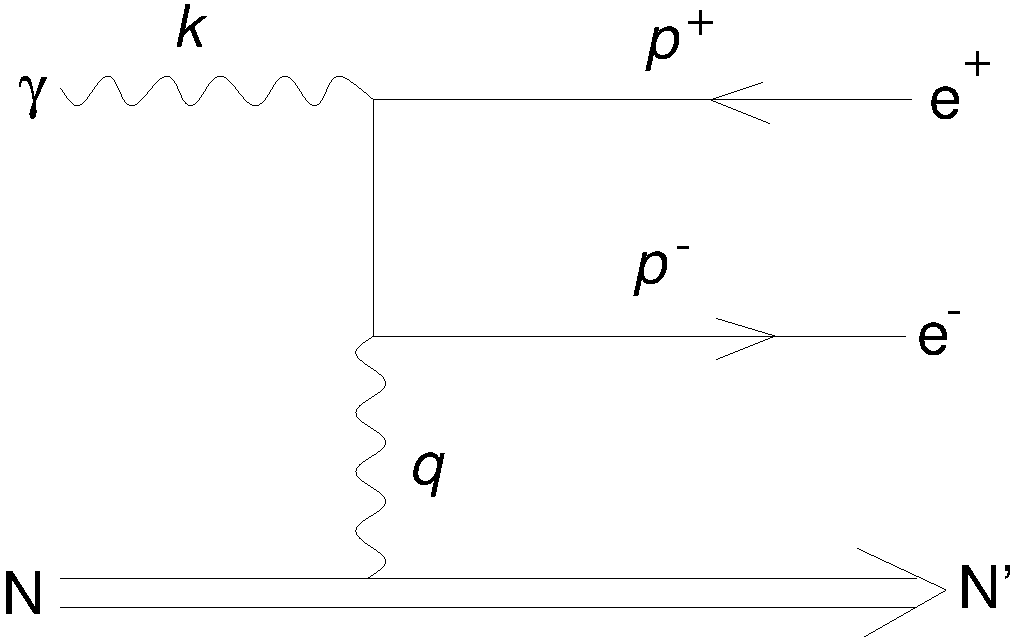
\includegraphics[height=8cm,width=12cm]{figures/pair}
\caption{\label{pair_fig} Feynman diagram for the pair
production process}
%\end{center}
\end{figure}
The triplet production process is similar but the interaction
takes place with one of the atomic electrons which receives
sufficient energy to be set free (so that there are 3 secondary electrons
produced in the interaction). By default
the triplet production process is
\index{triplet production}
not simulated explicitly but taken into account in an approximate
way by using the total pair+triplet cross section to
sample distances to subsequent pair production collisions.
By default EGSnrc adopts the cross sections used in EGS4, {\em i.e.}
%total cross sections taken from ??? and
extreme relativistic first Born approximation
(Coulomb corrected above 50 MeV)
differential cross sections  as formulated in the article by
Motz, Olsen and Koch \cite{Mo69}. For a photon energy
$k$ incident on the nucleus with the atomic number $Z$, the
differential pair production cross section is
\begin{eqnarray}
\label{pair-e}
& & {{\rm d}\sigma_{\rm pair}(Z,k,E_+) \over {\rm d}E_+}  =
{A_{\rm p}'(Z,k) r_0^2 \alpha Z (Z + \xi(Z) ) \over k}
\\ & & \quad
\left\{ \left( E_+^2 + E_-^2 \right) \left[ \phi_1(\delta) -
{4 \over 3} \ln Z  - 4 \tilde{f}_c(k,Z) \right] +
{2 \over 3} E_+ E_- \left[ \phi_2(\delta) -
{4 \over 3} \ln Z  - 4 \tilde{f}_c(k,Z) \right] \right\}
\nonumber
\end{eqnarray}
where $E_+$ and $E_-$ are the total energies of the
positron and electron,
\begin{equation}
\delta = 136 Z^{-1/3} 2 \Delta~,\quad \quad \Delta = {k m \over 2 E_+ E_-}
\end{equation}
and $\tilde{f}_c(Z)$ is the Coulomb correction,
\begin{equation}
\label{f_coulomb}
\tilde{f}_c(Z) =
\begin{cases}
f_c(Z), & k \ge 50~\text{MeV} \\
0, & \text{else}
\end{cases}
\end{equation}
where $f_c(Z)$ was derived by
Davies, Bethe and Maximon \cite{Da54},
\begin{equation}
\label{f_coulomb1}
f_c(Z) = a^2 \sum_{\nu=1}^\infty {1 \over \nu (\nu^2 + a^2)}, \quad
a = \alpha Z~.
\end{equation}
The empirical correction factor $A_{\rm p}'(k,Z)$ is
introduced in order to improve the total pair production
cross section at lower energies and is defined
as ``The best estimate of the total cross section
available divided by the total cross section resulting
from the integration of Eq. (\ref{pair-e}) with
$A_{\rm p}'(k,Z)=1$''. For energies above
50 MeV $A_{\rm p}'$ is taken to be unity, for
energies below 50 MeV the total pair+triplet cross sections compiled
by Storm and Israel \cite{SI70} are used.
The replacement $Z^2 \to Z (Z + \xi(Z))$ takes
into account the triplet production process, where $\xi(Z)$,
evaluated by the PEGS4 function {\tt XSIF},  is given by
\index{XSIF}
\begin{equation}
\xi(Z) = {L_{\rm rad}'(Z) \over L_{\rm rad}(Z) - f_c(Z)}
\end{equation}
where $f_c(Z)$ is defined in Eq. (\ref{f_coulomb}) and
$L,L'$ are Tsai's radiation logarithms \cite{Ts74},
\index{Tsai's radiation logarithms}
\begin{eqnarray}
L_{\rm rad}'(Z) & = &
\left\{
\begin{array}{r@{\quad , \quad}l}
\ln(1194\,Z^{-2/3}) &~~\mbox{if}~~~Z > 4 \\
6.144 & ~~\mbox{if}~~~Z = 1 \\
5.621 & ~~\mbox{if}~~~Z = 2 \\
5.805 & ~~\mbox{if}~~~Z = 3 \\
5.924 & ~~\mbox{if}~~~Z = 4
\end{array} \right. \nonumber \\
L_{\rm rad} & = &
\left\{
\begin{array}{r@{\quad , \quad}l}
\ln(184.15\,Z^{-1/3}) &~~\mbox{if}~~~Z > 4 \\
5.310 & ~~\mbox{if}~~~Z = 1 \\
4.790 & ~~\mbox{if}~~~Z = 2 \\
4.740 & ~~\mbox{if}~~~Z = 3 \\
4.710 & ~~\mbox{if}~~~Z = 4
\end{array} \right.
\end{eqnarray}
The functions $\phi_1(\delta)$ and $\phi_2(\delta)$, which
account for screening effects, are
given by
\begin{equation}
\begin{split}
\phi_1(\delta) & = 4 \int\limits_\Delta^1 {{\rm d}q \over q^3}
(q - \Delta)^2 \Big[1 - F(q,Z) \Big]^2 + 4 + {4 \over 3} \ln Z~,
\\
\phi_2(\delta) & = 4 \int\limits_\Delta^1  {{\rm d}q \over q^4}
\Big[q^3 - 6 \Delta^2 q \ln \left({q \over \Delta}\right) + 3 \Delta^2 q
-4 \Delta^3 \Big] \Big[1 - F(q,Z) \Big]^2 + {10 \over 3} + {4 \over 3} \ln Z
\end{split}
\end{equation}
where $q$ is the momentum transfer and $F(q,Z)$ the corresponding
atomic form factor for an atom with atomic
number $Z$. For a Thomas-Fermi potential $\phi_1(\delta)$
and $\phi_2(\delta)$ are independent of $Z$ and Butcher and
Messel have approximated them \cite{BM60} as
\begin{eqnarray}
\label{pair_phi}
\phi_1(\delta) & = & \left\{
\begin{array}{r@{\quad , \quad}l}
20.867 - 3.242 \delta + 0.625 \delta^2 & \delta \le 1 \\
21.12 - 4.184 \ln(\delta + 0.952) & \delta > 1
\end{array}
\right. \\
\phi_2(\delta) & = & \left\{
\begin{array}{r@{\quad , \quad}l}
20.029 - 1.93 \delta - 0.086 \delta^2 & \delta \le 1 \\
\phi_1(\delta) & \delta > 1
\end{array}
\right.
\end{eqnarray}

The differential pair production cross section for compounds
and mixture is derived from the independent atom approximation
and can be approximately written in the same form as Eq. (\ref{pair-e})
but replacing
\begin{eqnarray}
\label{pair_replace}
Z (Z + \xi(Z)) \quad & \mbox{with} & \quad Z_{\rm eff}^2 \equiv
\sum p_i Z_i (Z_i + \xi(Z_i) )
\nonumber \\
{1 \over 3} \ln Z + \tilde{f}_c(k,Z) \quad & \mbox{with} & \quad
Z_V \equiv \sum p_i
Z_i (Z_i + \xi(Z_i) ) \left[ {1 \over 3} \ln Z_i + \tilde{f}_c(k,Z_i) \right]
\nonumber \\
\delta \quad & \mbox{with} & \quad \delta_C 2 \Delta~,\quad
\delta_C \equiv {136 \over Z_{\rm eff}^2}
\sum p_i Z_i (Z_i + \xi(Z_i) ) Z_i^{-1/3}
\end{eqnarray}
where $p_i$ is the normalized fraction of atoms of type $i$ in
the molecule.

It is worth noticing that, due to the use of the extreme
relativistic approximation,  the differential cross
section as defined in Eq. (\ref{pair-e}) becomes inaccurate
for energies close to the threshold energy for pair production
(2 $\rm m$ ).
%and breaks down altogether for energies below
%2.1 MeV.
In the EGS4 implementation, the entire photon energy
was given to one of the pair particles for $k \le 2.1$ MeV.
We have defined a macro {\tt \$SELECT-LOW-ENERGY-PAIR-PRODUCTION}
which, in its default replacement, samples $E_+$ uniformly
in the allowed range $m \cdots k/2$. If the user is aware
of a better approach, this simplistic treatment can be
modified by the appropriate replacement of this macro.
\index{\$SELECT-LOW-ENERGY-PAIR-PRODUCTION}

\paragraph{NRC pair cross sections}\hfill
\index{pair cross sections!NRC}

In a more recent addition to EGSnrc, the user has the option
to specify use of a library of differential pair cross sections created
at the NRC. These cross sections are based on the exact partial-wave-analysis
calculations by {\O}verb{\o}, Mork and Olsen (OMO) \cite{Ov73} for the
unscreened nuclear potential modified by a multiplicative screening correction.
The main difficulty in creating this data library, which provides cross
sections up to 85 MeV for all elements between 1 and 100, consisted in finding
numerically stable approaches for performing the PWA summation for energies
above a few MeV (the OMO paper \cite{Ov73} only contains results up to 5.1 MeV).
Note that these cross sections take into account the asymmetry in the
positron-electron energy distribution and eliminate the need
for the {\tt \$SELECT-LOW-ENERGY-PAIR-PRODUCTION} macro mentioned
above.

In order to make use of the NRC pair cross sections, the user
\index{pair\_nrc}
must set the variable {\tt pair\_nrc}=1.  Note that
{\tt pair\_nrc} is part of the {\tt COMIN/BREMPR} common block
(see Section~\ref{common_blocks} of this report).

\paragraph{Explicit simulation of triplet production}\hfill
\index{triplet production}

In a more recent addition to EGSnrc, the user has the option
to explicitely simulate triplet production events according to the
first Born approximation result first derived by Votruba \cite{Vo48}
and later by Mork \cite{Mo67}. Due to the 3 particle final state the
expression for the differential triplet production cross section
is very complicated and so not reproduced here. It is worth
noting that the published expressions most likely contain typos
because their direct implementation in a computer program
lead to meaningless results ({\em e.g.} negative cross section within
the kinematically allowed range of energies and directions).
The triplet production cross section was therefore re-derived using
the CompHEP package, its results were manipulated using Mathematica and
were then output directly to Fortran code.

In order to turn on explicit simulation of triplet events, the user
\index{itriplet}
mist set the variable {\tt itriplet}=1. Note that
{\tt itriplet} is part of the {\tt COMIN/BREMPR} common block
(see Section~\ref{common_blocks} of this report).

The technique for sampling random directions and energies from
the differential triplet cross section is very involved.
Its detailed description awaits a future version of this report.


\paragraph{Simulation of pair production, particle energies}\hfill
\index{pair production!simulation of}

When the NRC pair differential cross section tabulations are used,
an alias table is employed for picking the positron energy.
For the default Bethe-Heitler cross sections,
the sampling algorithm implemented in EGS4 becomes extremely
inefficient as the incident photon energy approaches the
threshold energy. This is due to the following two facts:
(i) The electron and positron energies, $E_-$ and $E_+$,
are sampled in the range $0\cdots k/2$, the allowed
range becomes a small fraction of the above interval for
$k \to 2 m$. (ii) The rejection functions used are normalized
to their maximum at $\delta = 0$. For photon energies that
are not much larger than $2 m$ the actual possible maximum
is much smaller.

\index{EGS4}
We have therefore slightly modified the EGS4 pair production sampling algorithm to improve
its efficiency. If we define the functions
\begin{eqnarray}
B(\delta) & = & 3 \Big[ \phi_1(\delta) - 4 Z_V \Big] -
\Big[ \phi_2(\delta) - 4 Z_V \Big] \nonumber \\
C(\delta) & = & 3 \Big[ \phi_1(\delta) - 4 Z_V \Big] +
\Big[ \phi_2(\delta) - 4 Z_V \Big]
\end{eqnarray}
which will serve as rejection functions, and make
a change of variables,
\begin{equation}
\varepsilon  = {E_+ - m \over k - 2 m}~,
\end{equation}
the differential pair production cross section can be
rewritten as
\begin{equation}
{{\rm d} \sigma_{\rm pair} \over {\rm d} \varepsilon} =
N \left\{ {B(\delta) \over B_{\rm max}} + \left(1 - {2 m \over k} \right)^2
{A_{\rm max} \over 3 B_{\rm max}} A(\delta)
\left[ 12 \left(\varepsilon - \frac{1}{2} \right)^2 \right] \right\}
\end{equation}
where $N$ combines all constant factors that are irrelevant for
the sampling algorithm and $A_{\rm max}$ and $B_{\rm max}$ are
the maxima of the rejection functions $A(\delta)$ and $B(\delta)$,
\begin{equation}
A_{\rm max} = A\left({4 \delta_C m \over k}\right)~, \quad \quad
B_{\rm max} = B\left({4 \delta_C m \over k}\right)~.
\end{equation}
The sampling algorithm, which determines the energy
of the lower energy ``electron'' is then as follows:
\begin{enumerate}
\item
Calculate $A_{\rm max}$, $B_{\rm max}$ and $\alpha$,
\begin{equation}
\alpha = {1 \over 1 + (1 - 2 m/k)^2 A_{\rm max}/3/B_{\rm max}}
\end{equation}
To save time at high energies, use $A_{\rm max} = A(0)$ and
$B_{\rm max} = B(0)$ for $k \ge 50$~MeV.
\item
Draw a random number $r_1$
\item
If $r_1 > \alpha$, then sample $\varepsilon$
from $12 (\varepsilon - 1/2 )^2$, {\em i.e.}
\begin{equation}
\varepsilon = \frac{1}{2} \left(1 - \mbox{Max}\{r_2,r_3,r_4\}\right)
\end{equation}
and use $A(\delta)/A_{\rm max}$ as a rejection function in step 5
\item
Else, sample $\varepsilon$ uniformly, {\em i.e.}
\begin{equation}
\varepsilon = \frac{1}{2} r_2
\end{equation}
and use $B(\delta)/B_{\rm max}$ as a rejection function in step 5
\item
Calculate $\delta$ and the rejection function $R$ = $A(\delta)/A_{\rm max}$ or
$B(\delta)/B_{\rm max}$
\item
If $r_5 < R$, accept $\varepsilon$, else go to step 2.
\end{enumerate}

\begin{figure}[h]
%\setlength{\vsize}{12cm}
%\setlength{\abovecaptionskip}{0.5in}
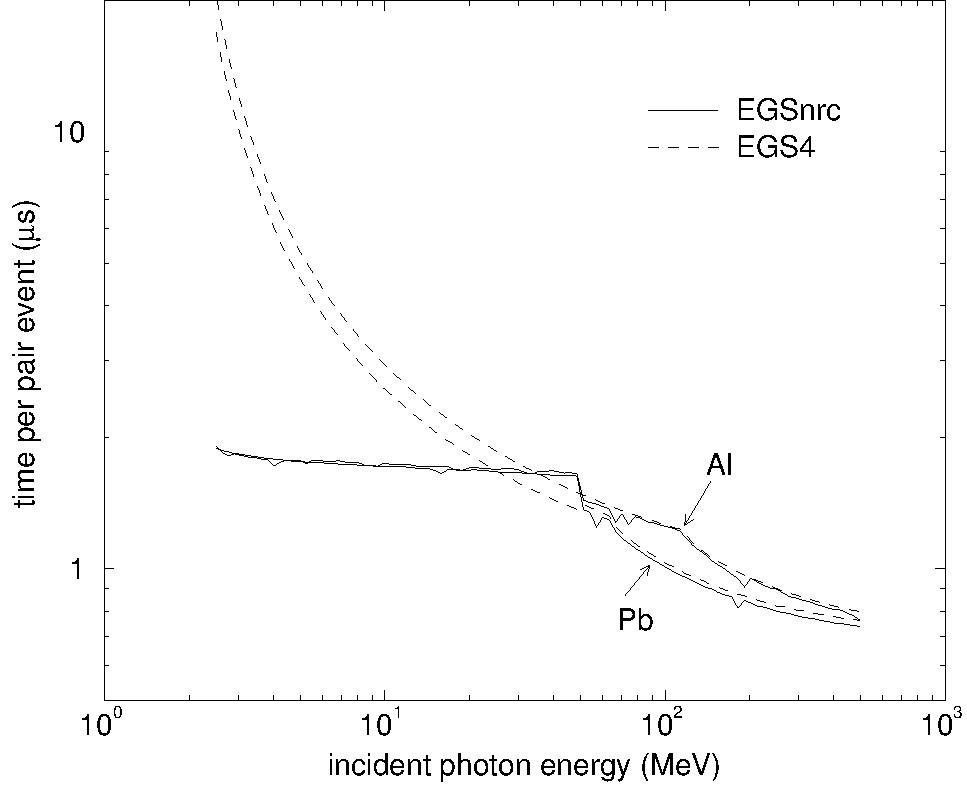
\includegraphics[height=12cm,width=12cm]{figures/pair_times}
\caption[CPU time for pair sampling]{\label{pair_times}
CPU time in $\mu$s on a 500 MHz PIII computer to sample a pair energy.}
\end{figure}

Fig. \ref{pair_times} shows the CPU time in $\mu$s on a 500 MHz PIII computer
running Linux necessary to sample a pair energy using the
algorithms discussed here (solid lines) and the original EGS4
algorithm (dashed lines) for aluminum and lead as a function
of the incident photon energy (this is just the time for
energy sampling, excluding angle sampling and rotations). Note
the logarithmic scale and the dramatic increase in CPU time for
the EGS4 algorithm and a photon energy less then 20 or 30 MeV.
The discontinuity in the EGSnrc algorithm around $50$~MeV
is due change in the
approach to calculate $A_{\rm max}$ and $B_{\rm max}$  (see item 1).

\paragraph{Simulation of pair production, particle angles}\hfill
\index{pair production!angular distribution}

\index{Bielajew, Alex} \index{EGS4}
In the original EGS4 version electrons and positrons were
produced at a fixed polar angle $\theta_{\pm}$ with respect to the direction
of the incoming photon given by $\theta_{\pm}=m/k$. This approach
was subsequently improved as discussed in PIRS Report 0287
\cite{Bi91} which introduced the {\tt \$SET-PAIR-ANGLE} macro
as an NRC extension to the EGS4 system.
This macro is now included in the EGSnrc system. The angle
selection procedure is controlled by the variable
{\tt IPRDST} (part of the {\tt COMIN/EDGE} common block--
see Section~\ref{common_blocks}) which can assume the following values:
\index{IPRDST}
\begin{itemize}
\item[]{\tt IPRDST=0}: The original EGS4 approach is used,
{\em i.e.} $\theta_{\pm}=m/k$
\item[]{\tt IPRDST=1}: The leading order term of the angular distribution
is employed, {\em i.e.}
\begin{equation}
\label{pair_ang1}
{{\rm d} \sigma \over {\rm d} \Omega_\pm} = N
{1 \over (1 - \beta_\pm \cos \theta_\pm)^2}
\end{equation}
where $N$ is again a normalization constant and $\beta_\pm$ denotes
the velocity of the positron or electron in units of the speed of light.
\item[]{\tt IPRDST=2}: The formula 3D-2003 of the article by
Motz {\em et al.} \cite{Mo69} is used, which is the cross section, differential
\index{IPRDST}
in electron/positron energy and angle:
\end{itemize}
\begin{equation}
\label{pair_ang_2}
\begin{split}
{{\rm d} \sigma \over {\rm d} E_\pm {\rm d} \Omega_\pm} & =
{N \over (u^2+1)^2 }
\left\{ -(E_+ - E_-)^2 - {16 u^2 E_+ E_- \over (u^2 + 1)^2} +
\left[ E_+^2 + E_-^2 + {4 u^2 E_+ E_- \over (u^2 + 1)^2} \right]
\ln M(k,E_\pm,u) \right\} \\
u & =  E_\pm \theta_\pm~, \quad {1 \over M(k,E_\pm,u)} =
\left({k \over 2 E_+ E_-} \right)^2 + \left( { Z_{\rm eff}^{1/3} \over
111 (u^2 + 1)^2 } \right)^2
\end{split}
\end{equation}
\begin{itemize}
\item[\phantom{\tt IPRDST=2}]
where all energies are measured in units of $m$.
Note that Eq. (\ref{pair_ang_2}) is based on an extreme relativistic,
small angle approximation where
\begin{equation}
\begin{split}
(1 - \beta_\pm \cos \theta_\pm)^2 & \approx
\left[1 - \beta_\pm \left(1 - \frac{\theta_\pm^2}{2}\right) \right]^2
= (1 - \beta_\pm)^2 \left[ 1 - {\beta_\pm \over 1 - \beta_\pm}
\frac{\theta_\pm^2}{2} \right]^2 \\
& \approx  (1 - \beta_\pm)^2 (1 + u^2)^2~.
\end{split}
\end{equation}
Perhaps, it would be a good idea to replace $1+u^2$ with
$1 - \beta_\pm \cos \theta_\pm$ in the denominator outside
of the curled brackets of Eq. (\ref{pair_ang_2}), but
we have not undertaken this modification.
\end{itemize}

The sampling algorithm for Eq. (\ref{pair_ang_2}) is discussed
extensively in Ref. \cite{Bi91}.
\index{Bielajew, Alex}
%.
It should be noted that
this algorithm becomes progressively more inefficient with
increasing energies. Given this fact and the approximations
involved which make its use questionable at low energies,
we have chosen {\tt IPRDST=1} as the default
pair angle selection scheme in EGSnrc. The generation
of electron and positron polar angles from the
distribution (\ref{pair_ang1}) is trivial, it
is accomplished by
\index{IPRDST}
\begin{equation}
\cos \theta_\pm = {2 r - 1 + \beta_\pm \over \beta_\pm (2 r -1 ) + 1}
\end{equation}
where $r$ is an uniformly distributed random number between zero and
unity. As pair-production is a three-body process, separate polar
angles for the electron and positron are needed. The two
azimuthal angles are chosen to be opposite. This is,
strictly speaking, not correct, but due to lack of a better
alternative, adopted from the original EGS4 version.

\paragraph{Russian Roulette for pair production events} \hfill
\index{Russian Roulette}
\index{variance reduction!Russian Roulette}
\index{pair production!Russian Roulette}

It is wasteful to simulate all pair production events if
the user intends to play Russian Roulette with electrons
set in motion in photon interactions. We have therefore implemented
an EGSnrc internal Russian Roulette scheme which is turned on
by setting the flag {\tt i\_play\_RR} which is in {\tt
COMIN/EGS-VARIANCE-REDUCTION/}
to 1. The survival probability for the electrons is
{\tt prob\_RR}, also in {\tt COMIN/EGS-VARIANCE-REDUCTION/}.
If {\tt i\_play\_RR} is set, the following actions are
taken at the beginning of subroutine {\tt PAIR}:
\index{EGS-VARIANCE-REDUCTION}
\index{prob\_RR} \index{i\_play\_RR}
\begin{enumerate}
\item
Pick a random number $r$
\item
If $r > $~{\tt prob\_RR}, reduce the stack size by one, return
to {\tt PHOTON} ({\em i.e.} save the simulation of the pair event).
If the stack becomes empty, a zero weight, zero energy photon
is left on the stack so that the {\tt PHOTON} routine can exit
properly.
\item
If $r < $~{\tt prob\_RR}, increase the weight of the current photon by
1/prob\_RR and simulate the pair event as usual.
\end{enumerate}
For more discussion of Russian Roulette see sections~\ref{rusrou} and
\ref{step_5b}.

\subsubsection{Incoherent (Compton) scattering}
\setcounter{equation}{0}
\label{compton}
\index{bound Compton scattering}
\index{Compton scattering}
\index{incoherent scattering}
\index{cross section!incoherent}

\paragraph{Cross section}\hfill

The Feynman diagram for the Compton scattering process is
shown in Fig. \ref{compt_fig}. The circle in the line
of the incoming atom A indicates that the electron
\begin{figure}[h]
%\begin{center}
%\setlength{\hsize}{15cm}
%\setlength{\vsize}{8cm}
%\setlength{\abovecaptionskip}{0.5in}
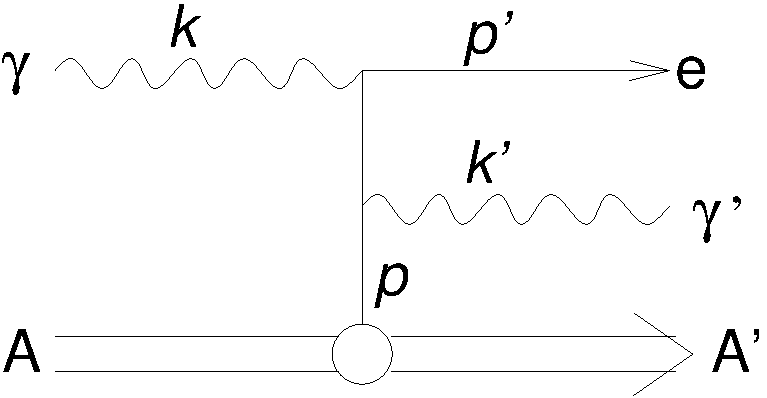
\includegraphics[height=8cm,width=12cm]{figures/compt}
\caption{\label{compt_fig} Feynman diagram for the Compton process}
%\end{center}
\end{figure}
is initially bound to the atom and represents the probability
that an atomic electron with a four-momentum $p = (E,\vec{p})$
interacts with the incoming photon with a four-momentum
$k=(k,\vec{k})$ into a final $e^-\gamma'$ state given by
$k'=(k',\vec{k'})$ and $p'=(E',\vec{p}')$.
To simplify the notation, all energies will be measured
in units of the electron's rest energy $m$ and all momenta
in units of $m/c$ in the following equations of this
section.

\index{Klein-Nishina}
If the binding to the atom is neglected and the electron
is considered to be initially at rest ({\em i.e} $p = (1,0,0,0)$),
the cross section for the process is given by the Klein-Nishina
formula \cite{KN29},
\begin{equation}
{{\rm d} \sigma_{\rm KN} \over {\rm d} \cos \theta} = \pi r_0^2 Z~
X_{\rm KN}~, \quad \quad X_{\rm KN} =
\left({k_c \over k} \right)^2
\left[ {k_c \over k} + {k \over k_c} - \sin^2 \theta \right]
\end{equation}
where $\theta$ is the polar angle of the scattered photon with
respect to the initial direction and $k_c$ is the energy
of a photon scattered at an angle $\theta$
by free electrons at rest,
\begin{equation}
k_c = {k \over 1 + k (1 - \cos \theta)}
\end{equation}
\index{Doppler broadening}
\index{incoherent scattering!binding effects}
\index{incoherent scattering!Doppler broadening}
The treatment of the Compton process in EGS4 is based on these
equations with $k' = k_c$. In EGSnrc we have included binding effects and
Doppler broadening according to the impulse approximation (IA)
\cite{Ri75}. The IA assumes that the potential in which the
target electrons move is constant so that their states can
be represented by plane waves. The double differential
cross section for photon scattering into the final state
$k' = (k', k' \sin \theta \cos \phi, k' \sin \theta \sin \phi, \\
k' \cos \theta)$ is given by (Eq. (15) of Ref. \cite{RB82})
\begin{equation}
\label{comp_cs1}
{{\rm d}^2 \sigma_{\rm comp} \over {\rm d}k' {\rm d}\Omega} =
{r_0^2 \over 2} {k' \over k q} \Big[1 + p_z^2 \Big]^{-1/2} X J(p_z)
\end{equation}
where $\Omega$ is the solid angle $(\theta,\phi)$ and where
\begin{itemize}
\item
$q$ is the modulus of the momentum transfer vector
$\vec{q} = \vec{k'} - \vec{k}$,
\begin{equation}
q = \sqrt{k^2 + k^{\prime 2} - 2 k k' \cos \theta}
\end{equation}
\item
$p_z$ is the projection of the initial electron momentum
on the direction of $\vec{q}$,
\begin{equation}
\label{comp_pz}
p_z = {\vec{p} \cdot \vec{q} \over q} =
{k k' (1 - \cos \theta) - k + k' \over q}
\end{equation}
Note that the above equation is derived from a non-relativistic
approximation and requires $|p_z| \le 1$.
\item
$X$ is defined as
\begin{eqnarray}
X & = & {R \over R'} + {R' \over R} +
2 \left(\frac{1}{R} - \frac{1}{R'} \right)
+ \left(\frac{1}{R} - \frac{1}{R'} \right)^2 \nonumber \\
R & = & k \left[ \sqrt{1 + p_z^2} + {k - k' \cos \theta \over q} p_z \right]
\nonumber \\
R' & = & R - k k' (1 - \cos \theta)~.
\end{eqnarray}
Note that $R$ and $R'$ simplify to
\begin{equation}
R \approx k \left(1 + O(p_z) \right)~, \quad
R' \approx k \Big[1 - k_c (1 - \cos \theta ) \Big] \left(1 + O(p_z) \right)
\end{equation}
for $p_z \ll 1$. In this limit
\begin{equation}
X = X_{\rm KN} \left(1 + O(p_z) \right)
\end{equation}
\item
The function $J(p_z)$ is the Compton profile,
\begin{equation}
J(p_z) = \int {\rm d} p_x {\rm d} p_y | \psi(\vec{p}) |^2~,
\end{equation}
where $\psi(\vec{p})$ is the wave function of the bound electrons.
Extensive tables of atomic and shell-wise
\index{Compton profiles}
\index{incoherent scattering!Compton profiles}
Hartree-Fock Compton profiles for all
elements have been published by Biggs {\em et al} \cite{BM75}.
Following Brusa {\em et al} \cite{BS96},
contributions
from different electron shells are considered separately, so
that the atomic or molecular Compton profile is the sum
of one-electron shell Compton profiles $J_i(p_z)$, and binding effects
are taken into account by rejecting interactions that
transfer less energy to the electron than the binding energy $U_i$,
{\em i.e.}
\begin{equation}
J(p_z) = \sum Z_i J_i(p_z) \Theta(k - k' - U_i)~.
\end{equation}
Here, $Z_i$ is the occupation number of shell $i$ and
the $J_i$ have the normalization
\begin{equation}
\int\limits_{-\infty}^\infty {\rm d} p_z J_i(p_z) = 1
\end{equation}
\end{itemize}
With all this, and after changing the cross section
from differential in $k'$ to differential in $p_z$,
Eq. (\ref{comp_cs1}) can be written as
\begin{equation}
{{\rm d}^2 \sigma_{\rm comp} \over {\rm d}p_z {\rm d}\Omega} =
{r_0^2 \over 2} X_{\rm KN}
\left( \sum Z_i J_i(p_z) \Theta(k - k' - U_i) \right) F(k,\cos \theta, p_z)
\end{equation}
where the function $F(k,\cos \theta, p_z)$ combines all remaining
factors times ${\rm d}k'/{\rm d}p_z$,
\begin{equation}
F(k,\cos \theta, p_z) = \frac{k'}{k_c} \Big[ 1 + p_z^2 \Big]^{-1/2}
\frac{X}{X_{\rm KN}} \left(1 + \frac{k_c}{k} {k \cos \theta - k' \over q} p_z
\right)^{-1}
\end{equation}
Here, $k'$ is a function of $k, \cos \theta$ and $p_z$ and
follows from solving Eq. (\ref{comp_pz}) with respect to $k'$,
{\em i.e.}
\begin{equation}
\label{comp_kprime}
k' = {k_c \over 1 - p_z^2 \varepsilon^2 } \left[
1 - p_z^2 \varepsilon \cos \theta + p_z \sqrt{1 - 2 \varepsilon
\cos \theta + \varepsilon^2 \left(1 - p_z^2 \sin^2 \theta \right) }~ \right]~,
\quad \quad \varepsilon = \frac{k_c}{k}
\end{equation}
The incoherent scattering cross section, differential in
the photon scattering angle, is
\begin{equation}
\label{comp_sig_omega}
{{\rm d} \sigma_{\rm comp} \over {\rm d}\Omega} =
{r_0^2 \over 2}
%\left(\frac{k_c}{k} \right)^2 : must not be there, noted by Trent Hawkins
X_{\rm KN} S(k,\cos \theta)
\end{equation}
where
\begin{equation}
\label{comp_sincoh}
S(k,\cos \theta) =
\sum Z_i \Theta(k - U_i) S_i, \quad \quad
S_i = \int\limits_{-\infty}^{p_i} {\rm d} p_z J_i(p_z)
F(k,\cos \theta, p_z)
\end{equation}
\index{incoherent scattering function}
can be identified with the incoherent scattering function.
The upper limit of the $p_z$ integration for the $i$'th shell, $p_i$,
\begin{equation}
\label{comp_pi}
p_i = { k (k - U_i) (1 - \cos \theta) - U_i \over
\sqrt{ 2 k (k - U_i) (1 - \cos \theta) + U_i^2}}~,
\end{equation}
follows from Eq. (\ref{comp_pz}) with
$k' = k - U_i$ and assures that sufficient energy is transferred
to the electron to set it free. To first order, $S(k,\cos \theta)$
depends only on $k \sqrt{(1 - \cos \theta)/2}$ and so,
Namito {\em et al} \cite{Na94} use tabulated
incoherent scattering functions in their
extension of the EGS4 system to include binding effects
and Doppler broadening, when sampling the photon scattering angle.
This approach introduces a slight inconsistency in their treatment
of the Compton process.

As the Compton profiles are
strongly peaked around $p_z=0$, the main contributions
to the integral come from small $p_z$ values where
the function $F(k,\cos \theta, p_z)$ is very close
to unity and so, Brusa {\em et al} \cite{BS96} approximate
$S(k,\cos \theta)$ with
\begin{equation}
\label{comp_sincoh1}
S(k,\cos \theta) \approx S_A((k,\cos \theta) \equiv
\sum Z_i \int\limits_{-\infty}^{p_i} {\rm d} p_z J_i(p_z)
\Theta(k - U_i)
\end{equation}
for their implementation of binding effects and Doppler broadening
in the PENELOPE system \cite{Sa96}\footnote{They take
into account $F(k,\cos \theta, p_z)$, using its Taylor
expansion up to $O(p_z)$, for the sampling of $p_z$.}
\begin{figure}[h]
%\begin{center}
%\setlength{\vsize}{12cm}
%\setlength{\abovecaptionskip}{0.5in}
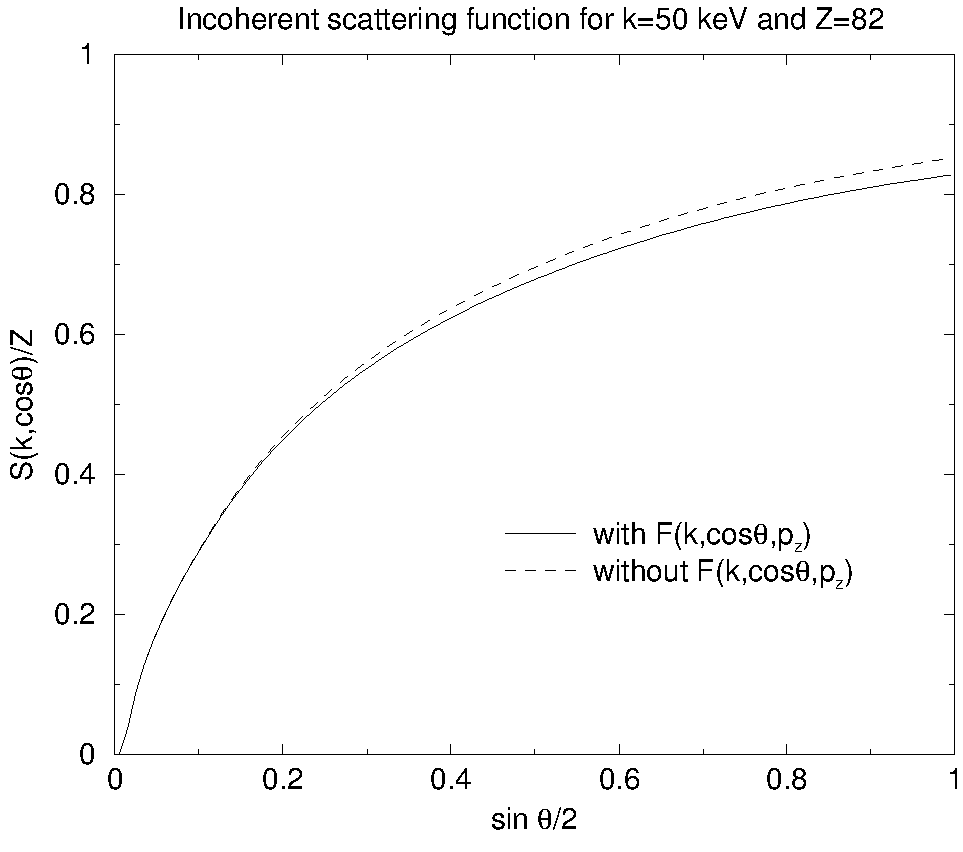
\includegraphics[height=12cm,width=12cm]{figures/sincoh}
%\end{center}
\caption[Incoherent scattering function]{\label{comp_sincoh_fig}
The incoherent scattering function for lead and $k=50$~keV
calculated from Eq. (\protect\ref{comp_sincoh}) (solid line)
and from Eq. (\protect\ref{comp_sincoh1}) (dashed line)
by numerical integration}.
\end{figure}
This approach introduces a small error at low energies
for high $Z$ materials as can be seen
in Fig. \ref{comp_sincoh_fig} which shows
$S(k,\cos \theta)$ for 50 keV photons in lead calculated
with or without taking into account $F(k,\cos \theta, p_z)$.

To minimize the amount of data necessary for
the simulation of the Compton process, and to make
the calculation of the incoherent scattering function ``on the fly''
possible, we use
the analytical approximations for the Compton profiles
$J_i(p_z)$ proposed by Brusa {\em et al} \cite{BS96}:
\begin{equation}
\label{comp_Japprox}
J_i(p_z) = J_{i,0} (1 + 2 J_{i,0} |p_z| ) \exp\left[\frac{1}{2} -
\frac{1}{2}\left(1 + 2 J_{i,0} |p_z| \right)^2\right]
\end{equation}
where $J_{i,0} \equiv J_i(0)$ is the value of the profile at
$p_z = 0$ obtained from the Hartree-Fock orbital \cite{BM75}.
In addition, we approximate $F(k,\cos \theta, p_z)$ by
\begin{equation}
\label{comp_Fapprox}
F((k,\cos \theta, p_z) = \left\{
\begin{array}{l@{\quad , \quad}l}
1 - \alpha p & p_z \le -p \\
1 + \alpha p_z & |p_z| < p \\
1 + \alpha p & p_z \ge p
\end{array} \right.
\end{equation}
where
\begin{eqnarray}
\label{comp_alpha}
\alpha & = & \frac{q_c}{k} \left(1 +
{k_c (k_c - k \cos \theta) \over q_c^2} \right)
\nonumber \\
q_c & = & \sqrt{k^2 + k_c^2 - 2 k k_c \cos \theta}~.
\end{eqnarray}
Equation (\ref{comp_Fapprox}) results from a Taylor series
expansion of $F(k,\cos \theta, p_z)$ up to $O(p_z)$. As this
approximation becomes inaccurate for large $p_z$ values
it is applied only for $|p_z| < p$, else the function values at
$\pm p$ are used. We have checked by numerical integration
of Eq. (\ref{comp_sincoh}) that the incoherent scattering function
calculated with the approximation (\ref{comp_Fapprox}) agrees
to better than 0.3\% with the incoherent scattering function
calculated using the exact expression for $F(k,\cos \theta, p_z)$
if $p = 0.15$ is used.

Combining now Eq. (\ref{comp_sincoh}), (\ref{comp_Japprox}) and
(\ref{comp_Fapprox}),  we obtain for $S_i$
%\begin{equation}
%S_i(k,\cos \theta) = \left\{
%\begin{array}{l@{\quad , \quad}l}
%(1 - \alpha p) {e^{-b} \over 2} & p_z \le -p \\
%(1 + \alpha p_z) {e^{-b} \over 2} - {\alpha \over 4 J_{i,0}}
%\sqrt{{\pi \over 2}} e^{1/2} \left[ \mbox{Erf} \left( 1 + 2 J_{i,0} p \over
%\sqrt{2} \right) - \mbox{Erf} \left(  1 + 2 J_{i,0} |p_z|
%\over \sqrt{2} \right) \right] & -p < p_z \le 0  \\
%1 - (1 + \alpha p_z) {e^{-b} \over 2} - {\alpha \over 4 J_{i,0}}
%\sqrt{{\pi \over 2}} e^{1/2} \left[ \mbox{Erf} \left( 1 + 2 J_{i,0} p \over
%\sqrt{2} \right) - \mbox{Erf} \left(  1 + 2 J_{i,0} |p_z|
%\over \sqrt{2} \right) \right] & 0 < p_z < p \\
%1 - (1 + \alpha p) {e^{-b} \over 2} & p_z \ge p
%\end{array} \right.
%\end{equation}
\begin{eqnarray}
\label{comp_Si}
& & S_i(k,\cos \theta) \nonumber \\
& = & (1 - \alpha p) {e^{-b} \over 2}~,\quad \mbox{if}~~p_i \le -p \nonumber \\
& = &
(1 + \alpha p_i) {e^{-b} \over 2} - {\alpha \over 4 J_{i,0}}
\sqrt{{\pi \over 2}} e^{1/2} \left[ \mbox{Erf} \left( 1 + 2 J_{i,0} p \over
\sqrt{2} \right) - \mbox{Erf} \left(  1 + 2 J_{i,0} |p_i|
\over \sqrt{2} \right) \right]~,\quad \mbox{else if}~~ p_i \le 0 \nonumber \\
& = &
1 - (1 + \alpha p_i) {e^{-b} \over 2} - {\alpha \over 4 J_{i,0}}
\sqrt{{\pi \over 2}} e^{1/2} \left[ \mbox{Erf} \left( 1 + 2 J_{i,0} p \over
\sqrt{2} \right) - \mbox{Erf} \left(  1 + 2 J_{i,0} |p_i|
\over \sqrt{2} \right) \right] ~,\quad \mbox{else if}~~ p_i < p \nonumber \\
& = &
1 - (1 + \alpha p) {e^{-b} \over 2} ~,\quad \mbox{else}
\end{eqnarray}
where
\begin{equation}
b = \frac{1}{2}\left(1 + 2 J_{i,0} |p_i| \right)^2 - \frac{1}{2}
\end{equation}
and $\mbox{Erf}$ is the error function. It is worth noticing that
$S_i$ is always less or equal to unity. This fact allows for
using it as a rejection function in the sampling algorithm discussed
in the next section.

The total incoherent scattering cross section $\sigma_{\rm comp}^{\rm (tot)}$
can be obtained
by a numerical integration over all scattering angles from
Eq. (\ref{comp_sig_omega}), (\ref{comp_sincoh}) and
(\ref{comp_Si}). To
avoid substantial changes of the data preparation program PEGS4,
we use instead the total Klein-Nishina cross section,
$\sigma_{\rm KN}^{\rm (tot)}$, while tracking the photons through
the geometry, and reject Compton interactions with the probability
$1-\sigma_{\rm comp}^{\rm (tot)}/\sigma_{\rm KN}^{\rm (tot)}$ once
at the interaction site (fictitious cross section method).
This rejection probability results automatically (without
calculating $\sigma_{\rm comp}^{\rm (tot)}$) from the sampling
algorithm, as we shall see in the next section.

\index{IBCMP}
Another advantage of this approach is that the user can
turn on or off binding effects and Doppler broadening
using the switch {\tt IBCMP} (included in the common
block {\tt COMIN/COMPTON-DATA}--see Section~\ref{common_blocks}),
without preparing two
separate material data files. The only additional data
needed to simulate incoherent scattering in the impulse
approximation are the Compton profile parameters
$J_{i,0}$, taken from the tabulations by Biggs {\em et al}
\cite{BM75}, and the occupation numbers $Z_i$ and
binding energies $U_i$ for all elements, taken from
Lederer and Shirley \cite{LS78}. These data are read in
in subroutine {\tt init\_compton} which is called from
{\tt HATCH}.
\index{init\_compton}

\paragraph{Simulation of incoherent scattering events}\hfill
\index{incoherent scattering!simulation of}
\index{Compton scattering!simulation of}
\index{bound Compton scattering}

The incoherent scattering cross section, differential in
the photon scattering angle $\Omega = (\theta,\phi)$
and the Doppler broadening
parameter $p_z$, per interaction site sampled from the
total Klein-Nishina cross section is
\begin{eqnarray}
{{\rm d}^2 \sigma_{\rm comp} \over \sigma_{\rm KN}^{\rm (tot)}} & = &
\sum \frac{Z_i}{Z} \Theta(k - U_i)~ \sigma_i~ {\rm d} \Omega~ {\rm d} p_z
\\
\sigma_i~ {\rm d} \Omega~ {\rm d} p_z & = &
%\left( \int\limits_{-\infty}^{p_i} {\rm d} p_z J_i(p_z) F(k,\cos \theta,p_z)
%\right)~
S_i~
{{\rm d} \phi \over 2 \pi}~
{X_{\rm KN}(\cos \theta)~{\rm d} \cos \theta~ \over
\int\limits_{-1}^1 X_{\rm KN}(\cos \theta) {\rm d} \cos \theta }
~{ J_i(p_z) F(k,\cos \theta,p_z) \Theta(p_i - p_z) {\rm d} p_z \over
\int\limits_{-\infty}^{p_i} {\rm d} p_z J_i(p_z) F(k,\cos \theta,p_z) }
\nonumber
\end{eqnarray}
It is then clear that the following algorithm produces the
required number of rejections and samples the differential
cross section correctly, if the interaction is accepted:
\begin{enumerate}
\item
Sample the shell number $i$ using the probabilities $Z_i/Z$
\item
If the incident photon energy $k$ is smaller than the binding
energy $U_i$, reject the interaction,
else, sample $\cos \theta, \phi$ and $p_z$ using the differential
cross section $\sigma_i$ of the selected shell as follows:
\item
Sample the photon polar scattering angle $\theta$ using
\begin{displaymath}
P_1(\cos \theta) =
{X_{\rm KN}(\cos \theta)~{\rm d} \cos \theta~ \over
\int\limits_{-1}^1 X_{\rm KN}(\cos \theta) {\rm d} \cos \theta }
\end{displaymath}
which is a normalized probability distribution function (PDF). The method
for sampling $\cos \theta$ will be explained below.
\item
Calculate the maximum possible value of $p_z$, $p_i$, from
Eq. (\ref{comp_pi}), and $S_i$ from Eq. (\ref{comp_Si}).
\item
If a uniformly distributed random number is greater then $S_i$,
reject the interaction
\item
Sample $p_z$ from
\begin{displaymath}
P_2(p_z) =
{ J_i(p_z) F(k,\cos \theta,p_z) \Theta(p_i - p_z) {\rm d} p_z \over
\int\limits_{-\infty}^{p_i} {\rm d} p_z J_i(p_z) F(k,\cos \theta,p_z) }
\end{displaymath}
which is a normalized PDF for $p_z$. The sampling
technique employed for this distribution function is explained below.
\item
Sample the azimuthal scattering angle from ${\rm d}\phi/(2 \pi)$
\item
Calculate the energy $k'$ of the scattered photon from
Eq. (\ref{comp_kprime})
\item
The electron set in motion has then a kinetic energy of $k - k' - U_i$,
a polar scattering angle $\theta_e$ given by
\begin{equation}
\cos \theta_e = {k - k' \cos \theta \over
\sqrt{k^2 + k^{\prime 2} - 2 k k' \cos \theta} }
\end{equation}
and an azimuth opposite to the photon's azimuth.
\end{enumerate}
Note that if the user does not want to take into account binding
effects and Doppler broadening (the switch {\tt IBCMP} is set to zero)
the sampling algorithm consists of steps 3, 7 and 9 with
$k' = k_c$ and $U_i = 0$.
\index{IBCMP}

As the shell with which the interaction takes place is explicitly determined
in step 1, at the end of the sampling algorithm the vacancy created
by the Compton process is known. The relaxation of shell vacancies
\index{relaxations}
\index{atomic relaxations}
with binding energies above the specified transport threshold
energies is performed in subroutine {\tt relax} (see section \ref{relax}) and
may lead to the creation of additional fluorescent photons and
Auger and Coster-Kronig electrons on the stack. Many of the
EGS4 based user codes assume that the outcome of an incoherent scattering
process is a scattered photon and a Compton electron. This assumption
is obviously not satisfied for EGSnrc, the outcome of an incoherent
event may by any one of the following:
\begin{enumerate}
\item
The original photon, if the interaction was rejected due to the one
of the rejection criteria
\item
A scattered photon and a Compton electron, if all relaxation particles
had energies below the specified transport threshold energies
({\tt ECUT} and {\tt PCUT})
\item
A scattered photon, a Compton electron plus $n$ relaxation particles, else.
\end{enumerate}
See section~\ref{stack_status} (page~\pageref{stack_status}) for more
information.

Finally, the portion of the binding energy that resulted in the creation
of sub-threshold relaxation particles is made known to the user via
a call to the scoring routine {\tt AUSGAB} with the argument {\tt IARG=4}.
\index{AUSGAB}
\index{IARG!4}

We conclude this section with some details about steps 3, 4 and 6
of the sampling algorithm.

\underline{Step 3, sampling of $\cos \theta$}: Following
the EGS4 manual\cite{Ne85} we rewrite
the PDF $P_1$ in terms of $\varepsilon = k_c/k$,
\index{SLAC-265}
\begin{equation}
\label{comp_P1}
P_1(\varepsilon) = P_1(\cos \theta) {{\rm d}\varepsilon \over
{\rm d} \cos \theta} = N \left( \frac{1}{\varepsilon} + \varepsilon -
\sin^2 \theta \right)
\end{equation}
where $N$ is a normalization constant that is irrelevant for the sampling
algorithm. The minimum and maximum possible values for
$\varepsilon$, $\varepsilon_{\rm min}$ and $\varepsilon_{\rm max}$, follow
from $\cos \theta = -1$ and $\cos \theta = 1$, respectively, and are
given by
\begin{equation}
\varepsilon_{{\rm min}} = {1 \over 1 + 2 k}~, \quad \quad
\varepsilon_{{\rm max}} = 1~.
\end{equation}
Equation (\ref{comp_P1}) can be further rewritten as
\begin{equation}
P_1(\varepsilon) = N (\alpha_1 + \alpha_2) \left\{
{\alpha_1 \over \alpha_1 + \alpha_2}~
\left({1 \over \varepsilon \alpha_1} \right)
+ {\alpha_2 \over \alpha_1 + \alpha_2}~\left({ \varepsilon \over \alpha_2}
\right) \right\} \left[ 1 - {\varepsilon \sin^2 \theta \over 1 +
\varepsilon^2 } \right]
\end{equation}
with
\begin{equation}
\alpha_1  =  \ln \left(1 + 2 k \right)~, \quad \quad
\alpha_2  = {1 - \varepsilon_{\rm min}^2 \over 2}
\end{equation}
$1/\varepsilon/\alpha_1$ and $\varepsilon/\alpha_2$ are
normalized PDFs, they can be used to sample $\varepsilon$
with the probability $\alpha_1/(\alpha_1 + \alpha_2)$ and
$\alpha_2/(\alpha_1 + \alpha_2)$, respectively. The expression
of the square brackets has a maximum of unity for
$\varepsilon = 1$ ($\sin \theta = 0$) and is thus
a valid rejection function. The sampling algorithm is then as follows:
\begin{itemize}
\item[3.1]
Calculate $\varepsilon_{\rm min}, \alpha_1, \alpha_2$ and
$w = \alpha_1/(\alpha_1 + \alpha_2)$
\item[3.2]
Pick three random numbers $r_1, r_2$ and $r_3$
\item[3.3]
If $r_1 \le w$,
\begin{equation}
\varepsilon = \varepsilon_{\rm min} \exp( r_2 \alpha_1 )~,
\end{equation}
else,
\begin{equation}
\varepsilon = \sqrt{ \varepsilon_{\rm min}^2 + 2 r_2 \alpha_2}
\end{equation}
\item[3.4]
Calculate the rejection function ($g$), if $r_3 > g$ go to step 3.2
\item[3.5]
Deliver $\varepsilon$ (and $\cos \theta$)
\end{itemize}
The efficiency of this algorithm
goes to unity for $k \to \infty$ and therefore this is
the most efficient algorithm at high incident photon energies.
For $k \to 0$, the efficiency approaches $2/3$. In addition,
the necessity to calculate a logarithm and an exponential function,
two CPU intensive calculations, makes this algorithm slower than
a simple rejection technique with a uniform sampling of $\varepsilon$.
The rejection function in this case is given by
\begin{equation}
g = \frac{1}{g_{\rm max}} \left( {1 \over \varepsilon} + \varepsilon -
\sin^2 \theta \right)~, \quad \quad g_{\rm max} =
{1 \over \varepsilon_{\rm min}} + \varepsilon_{\rm min}
\end{equation}
and the algorithm is as follows
\begin{itemize}
\item[3.1]
Calculate $\varepsilon_{\rm min}$ and $g_{\rm max}$
\item[3.2]
Pick two random numbers $r_1$ and $r_2$
\item[3.3]
Set
\begin{equation}
\varepsilon = r_1 + (1 - r_1) \varepsilon_{\rm min}
\end{equation}
and calculate $g$
\item[3.4]
If $r_2 > g$, go to step 3.2
\item[3.5]
Deliver $\varepsilon$ (and $\cos \theta$)
\end{itemize}
The efficiency of this algorithm is $2/3$ for low energies and
decreases with increasing $k$. Because there are no CPU intensive
calculations involved, it is faster up to $k \sim 2$ and
used by EGSnrc in this energy range.

\underline{Step 4, calculation of $S_i$}: The calculation of
$S_i$ requires two numerically intensive operations, the
computation of $\exp(-b)$ and the calculation of the error
function that depends on $p_i$. The former is necessary for
the sampling of $p_z$ in step 6, the latter can be avoided
by using an approximate formula for $\mbox{Erf}$
(Eq. 7.1.25 of Abramowitz and Stegun \cite{AS64}):
\begin{eqnarray}
& & e^{1/2} \mbox{Erf} \left( { 1 + 2 J_{i,0} |p_i| \over \sqrt{2} } \right)
= e^{1/2} - e^{-b} t (a_1 + a_2 t + a_3 t^2 ) \\
t & = & {1 \over 1 + 0.332673 (1 + 2 J_{i,0} |p_i|)}~, \quad a_1 = 0.34802~,
\quad a_2 = -0.0958798~, \quad a_3 = 0.7478556 \nonumber
\end{eqnarray}
which is accurate enough for our purposes.

\underline{Step 6, sampling $p_z$}:
$p_z$ can be sampled using $J_i(p_z)$ as a PDF and $F$ as a rejection
function. To determine the maximum of $F$ we note that $\alpha$
(given by Eq. (\ref{comp_alpha})) is always positive except for
a small $\cos \theta$-range for $k > 3$. For such high incident
photon energies the influence of $F$ is negligible and so
we ignore it if $\alpha < 0$ ({\em i.e.} we set $\alpha = 0$).
The maximum of the rejection function, $F_{\rm max}$, is then
\begin{equation}
F_{\rm max} =
\label{comp_Fmax}
 \left\{
\begin{array}{l@{\quad , \quad}l}
1 - \alpha p & p_z \le -p \\
1 + \alpha p_i & |p_i| < p \\
1 + \alpha p & p_i \ge p
\end{array} \right.
\end{equation}
and the algorithm for sampling $p_z$ as follows:
\begin{itemize}
\item[6.1]
Calculate $F_{\rm max}$ from Eq. (\ref{comp_Fmax})
\item[6.2]
Pick two random numbers, $r_1$ and $r_2$, calculate $r' = r_1 e^{-b}$
($e^{-b}$ is known from step 4 of the main algorithm)
\item[6.3]
Set
\begin{equation}
p_z = \left\{ \begin{array}{l@{\quad , \quad}l}
{1 - \sqrt{1 - 2 \ln [2 r']} \over 2 J_{i,0}} & r' < 1/2 \\
{\sqrt{1 - 2 \ln [2(1-r')]} - 1 \over 2 J_{i,0}} & r' \ge 1/2
\end{array} \right.
\end{equation}
\item[6.4]
Calculate $F(p_z)$, if $r_2 > F(p_z)/F_{\rm max}$, go to step 6.2
\item[6.5]
Deliver $p_z$
\end{itemize}

It is easy to see that the sampling of incoherent scattering events
with binding effects and Doppler broadening taken into account
requires substantially more numerical work compared to
the free electron case (using the Klein-Nishina cross section).
\begin{figure}[h]
%\setlength{\vsize}{12cm}
%\setlength{\abovecaptionskip}{0.5in}
%\epsfxsize = 12cm
%\epsfysize = 12cm
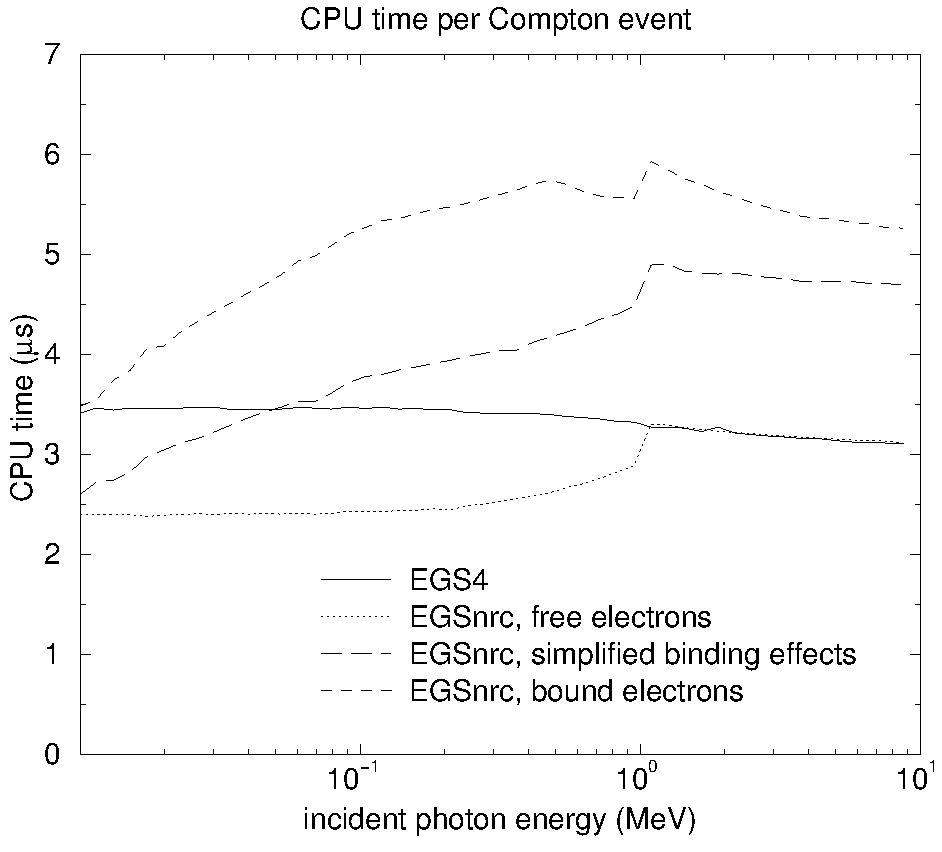
\includegraphics[height=12cm,width=12cm]{figures/comp_times}
\caption[CPU times for Compton sampling]{\label{comp_times}
CPU time in $\mu$s on a 500 MHz PIII computer to sample an incoherent
scattering event (including necessary rotations of particle directions).}
\end{figure}
Fig. \ref{comp_times} shows the CPU time per incoherent scattering event
for EGS4 (solid line), EGSnrc without (dotted line)
and with binding effects (dashed line) as a function of the incident
photon energy. The long dashed line would result if the function
$F(k,\cos \theta,p_z)$ was ignored. EGSnrc without binding effects is
faster than EGS4 for low photon energies due to the use of
the uniform sampling technique. The inclusion of binding effects
increases the CPU time per Compton event by not more than a
factor of two and so has only a minor effect on the overall simulation
time when electron transport is included. Binding effects and
Doppler broadening for coherent scattering are therefore turned
on by default in the {\tt block data} sub-program (the switch
{\tt IBCMP} is set to 3, {\tt norej}).
\index{IBCMP}

Since the 2009 release of EGSnrc, the user has the option to change
the EGSnrc behavior with respect to Compton interactions by
setting {\tt ibcmp=2} or {\tt ibcmp=3}.
When {\tt ibcmp=2}, binding effects are taken into account via an
incoherent scattering function, but there is no Doppler broadening.
This option was mainly added for the sake of being able to study the
effect of Doppler broadening by comparing simulations with
{\tt ibcmp=2} to {\tt ibcmp=1}. To select this option the user
must set {\tt Bound Compton scattering} to {\tt simple} in the
{\tt MC TRANSPORT PARAMETER} input block.
The {\tt ibcmp=3} option is the same as {\tt ibcmp=1}, but now the actual total
bound Compton cross section
is used and there are no rejections at run time. The addition of this option
was motivated by the complications associated with the initial bound
Compton scattering approach when using an un-weighting technique to compute
ion chamber correction factors for photon attenuation.
To select this option the user
must set {\tt Bound Compton scattering} to {\tt norej} in the
{\tt MC TRANSPORT PARAMETER} input block.

\index{Russian Roulette}
\index{variance reduction!Russian Roulette}
\index{incoherent scattering!Russian Roulette}
If the Russian Roulette option is turned on {\tt i\_play\_RR} set
to 1, electrons produced as a result of the Compton interaction
(the Compton electron and electrons from the relaxation of
the shell vacancy) are removed from the stack with the probability
{\tt prob\_RR}. If they survive, their weight is increased by
1/{\tt prob\_RR}.

\paragraph{Radiative Compton corrections}\hfill
\index{radiative Compton corrections}
\label{radc_corrections}

Recently, the code has been modified to also allow the user to include
radiative corrections for Compton scattering in the one-loop approximation.
These corrections are based on the original
Brown \& Feynman equations \cite{BF52}. The effect of loop corrections is to
reduce the cross section at large photon scattering angles. This is partially
offset by the addition of the double-Compton scattering process (two photons in
the final state). Devising an efficient technique for sampling energies and
directions from the double-Compton cross section is the most difficult part
in the implementation. The method is quite involved and its detailed description
awaits a future version of this report.

In order to turn on radiative corrections, the input variable
\index{radc\_flag}
\texttt{radc\_flag} (in the common block \texttt{COMIN/COMPTON-DATA}) must be set to 1.
This option can be enabled in applications which can read the \texttt{MC transport parameter}
input block from an input file (\texttt{*.egsinp}) via the input key:
\begin{verbatim}
   Radiative Compton corrections = on
\end{verbatim}
Moreover, one must include the file \texttt{\$(EGS\_SOURCEDIR)rad\_compton1.mortran} to the
list of MORTRAN sources to be built just before \texttt{\$(EGS\_SOURCEDIR)get\_inputs.mortran}.
Depending on the application type this is accomplished in different ways:

\begin{itemize}
 \item
  For all C++ applications one must edit the file \texttt{\$HEN\_HOUSE/specs/egspp1.spec}
  and include the above file in the definition of the \texttt{C\_ADVANCED\_SOURCES}
  variable if the application is derived from the \texttt{EGS\_AdvancedApplication} class or the
  \texttt{C\_SIMPLE\_SOURCES} variable for any application derived from the \texttt{EGS\_SimpleApplication} class.
 \item
  For a specific C++ application one could define the variable \texttt{CPP\_SOURCES} in the application's
  \texttt{Makefile} in the same manner as done above for the \texttt{C\_ADVANCED\_SOURCES}.
 \item
  For a \texttt{BEAMnrc} application one must edit the file \texttt{sources.make} located in the application's
  folder and include the above file in the definition of the \texttt{SOURCES} variable
  or the \texttt{LIB\_SOURCES} variable if this \texttt{BEAMnrc} application will be used as a particle source for
  another application.
 \item
  For a MORTRAN application named for instance \texttt{app} one must edit the corresponding file app.make located
  in the application's folder \texttt{\$EGS\_HOME/app} and include the above file
  in the definition of the \texttt{SOURCES} variable.
\end{itemize}

% Note that if radiative Compton corrections are to be used then the \texttt{Makefile} of
% the user code must be modified to include the file \texttt{\$(EGS\_SOURCEDIR)rad\_compton1.mortran}
% in the \texttt{SOURCES} list, just before\\
% \texttt{\$(EGS\_SOURCEDIR)get\_inputs.mortran}.

\paragraph{Total Compton cross sections}\hfill
\label{comp_xsect}
\index{bound Compton scattering!user-supplied cross sections}

As mentioned above, the total Compton cross section used in EGSnrc is obtained
from the theoretical expressions by integration of the differential cross sections.
Another recent addition to the EGSnrc code allows the user to supply their
own cross sections for bound Compton scattering. This option is only available
if the user is simulating bound Compton scattering
\index{IBCMP}
({\tt IBCMP}=1,2,3).  The cross sections
must be contained in a file\\
 {\tt \$HEN\_HOUSE/data/comp\_xsections\_compton.data},
where {\tt comp\_xsections} is the variable
(in common block {\tt COMIN/MEDIA}) holding the name as supplied
by the user.
\index{comp\_xsections}

\subsubsection{Photo-electric absorption}
\setcounter{equation}{0}
\label{photo}
\index{photo-electric absorption}

In the photo-electric absorption process a photon is
absorbed by an atom and an electron
is emitted with an energy given by the incident photon
energy minus its binding energy.
The atom, left in an excited state with a vacancy in the
ionized shell, relaxes via the emission of fluorescent photons and
Auger and Coster-Kronig electrons.

\index{fluorescent X-rays}
In the original default EGS4 implementation the emission of relaxation
particles following photo-electric absorption events was
ignored. This approach was later modified
to include the production of $K_\alpha$ and $K_\beta$ fluorescent
radiation. However, for incident photon energies below
the $K$-shell binding energy, the entire photon energy is
deposited locally. Another shortcoming of the EGS4 approach is
that the $K$-shell binding energy is always subtracted
from the energy of the electron set in motion, even though there
is a certain probability that the photo-absorption process
takes place with a shell other than the $K$-shell (for
high-$Z$ materials this probability is of the order of 20\%).
Finally, the use of the fluorescent option in EGS4 requires
the user to select an ``effective'' atomic number for each
material. The photo-absorption then always takes place with
this atomic number. The meaningful selection of an
``effective'' $Z$ proves to be a difficult task for mixtures, especially
when only a small fraction of a high-$Z$ element is present.

\index{cross section!photo-electric absorption}
Although this release of EGSnrc uses the total photo-absorption
cross sections from PEGS (which are taken from the
compilation by Storm and Israel \cite{SI70})
the simulation of the photo-absorption process
is completely changed and is controlled
by the flag {\tt IEDGFL}
(in the {\tt COMIN/EDGE} common block-see Section~\ref{common_blocks}). If {\tt IEDGFL} of the
region is non-zero, a detailed simulation is performed,
otherwise a simplified treatment of the photo-absorption process
is undertaken. The default setting of {\tt IEDGFL} is 1.
\index{IEDGFL}

\paragraph{Detailed simulation of photo-electric absorption}\hfill
\label{photo_detailed}
\index{photo-electric absorption!detailed simulation of}

\begin{enumerate}
\item
For compounds and mixtures, the first step is to sample the
atomic number of the element the
photon is interacting with.
If $Z_i$ denotes the atomic number of the $i$'th element in
the molecule, $p_i$ its stoichiometric index, and
$\sigma_{\rm ph}(k,Z)$ the photo-electric absorption
cross section for a photon of energy $k$ by an element
with atomic number $Z$, then the probability $w_i(k)$ that
the photon is absorbed by the element $Z_i$ is
\begin{equation}
w_i = {p_i \sigma_{\rm ph}(k,Z_i) \over \sum p_i \sigma_{\rm ph}(k,Z_i)}~.
\end{equation}
The sampling of the element therefore requires the knowledge of
all elemental photo-absorption cross sections at run time, not
just the total photo-absorption cross sections that comes from
the PEGS data set. To minimize the amount of additional data
required, we use fit formulas for the $\sigma_{\rm ph}(k,Z_i)$'s
which are accurate to within 1-2\% and have the form
\begin{eqnarray}
\sigma_{\rm ph}(k,Z) & = & \frac{A_K(Z)}{k} + \frac{B_K(Z)}{k^2} +
\frac{C_K(Z)}{k^{7/2}} + \frac{D_K(Z)}{k^4}~, \quad \mbox{if}~k \ge U_K(Z)
\\
%& = & \exp \left[A_j(Z) + B_j(Z) \ln k + C_j(Z) (\ln k)^2 + D_j(Z) (\ln k)^3
%\right]~, \quad \mbox{else if}~k \ge U_j(Z)
& = & \exp \left[A_j(Z) + B_j(Z) t + C_j(Z) t^2 + D_j(Z) t^3
\right]~, \quad \mbox{else if}~k \ge U_j(Z)
\nonumber
\end{eqnarray}
where $t = \ln k$ and where $U_K(Z)$ is the
$K$-shell binding energy and $U_j(Z)$ binding
energies for shells other then the $K$-shell. We have obtained The
coefficients $A_K, B_K, ...$ and $A_j, B_j, ...$
by fitting the photo-absorption cross sections from the {\tt XCOM} program
\cite{BH87} and are found in the file {\tt photo\_cs.data}
(only shells with a binding energy above 1 keV are included).
The algorithm to select the element that absorbs the
incident photon is then:
\begin{itemize}
\item[1.1] Calculate all $\sigma_{\rm ph}(k,Z_i)$ and
their sum
\item[1.2] Pick a random number $r_1$
\item[1.3] In a loop over the number of elements, calculate
$r_1 = r_1 - w_i$, if $r_1 \le 0$ exit the loop and take
$Z_i$ as the element interacting with the photon.
\end{itemize}
Note that, at least in principle,
\begin{displaymath}
\sum p_i \sigma_{\rm ph}(k,Z_i) = \sigma_{\rm ph}(k)
\end{displaymath}
where $\sigma_{\rm ph}(k)$ is the photo-absorption cross section
for the material under consideration. This cross section is
interpolated using the PEGS supplied data in the photon
transport routine in order to determine
the interaction type. One could make the element selection algorithm
more efficient by employing
\begin{itemize}
\item[1.1']
Pick a random number $r_1$
\item[1.2']
Set $i=1$
\item[1.3']
Calculate $\sigma_{\rm ph}(k,Z_i)$ and
$r_1 = r_1 - p_i \sigma_{\rm ph}(k,Z_i)/\sigma_{\rm ph}(k)$.
\item[1.4'] If $r_1 > 0$ and $i$ less then the number of elements,
then $i = i+1$, go to step 1.3'.
\item[1.5'] Deliver $i$.
\end{itemize}
as this saves the evaluation of one or more $\sigma_{\rm ph}(k,Z_i)$
(especially if elements are ordered by decreasing probability for
photo-absorption prior to the actual simulation). We have not
implemented this more efficient algorithm as the photo-absorption
cross section interpolated using the PEGS supplied data becomes
inaccurate around absorption edges. This potential improvement is
left for future releases of the system (which are anticipated to
not make use of PEGS data sets).
\item
Once the absorbing element is determined, the shell
with which the interaction takes place has to be sampled.
The probability $\nu_j$ that the photon is absorbed by the $j$'th shell
is close to energy independent for the $K$-shell but depends
on the incident photon energy for other shells. This means that
shell-wise photo-absorption cross sections would be required
to be available at run time in order to sample the shell
if one wanted to perform a complete modeling of the
photo-absorption process. In this release of the EGSnrc system
we use instead energy independent interaction probabilities $\nu_j$
which are determined as follows. If $\phi(k)$ is the
fluence of the photon radiation field, the number of photo-absorption
events by the element $Z$ per unit volume, $N$, is given by
\begin{equation}
N = n(Z) \int {\rm d} k \phi(k) \sigma_{\rm ph}(k,Z)
\end{equation}
where $n$ is the density of scattering centers.
The number of photo-absorptions by the shell $j$ of this
element per unit volume is
\begin{equation}
N_j = n(Z) \int {\rm d} k \phi(k) \sigma_{{\rm ph},j}(k,Z)
\end{equation}
where $\sigma_{{\rm ph},j}(k,Z)$ is the photo-absorption cross section
of the $j$'th shell. The ratio of $N_j$ to $N$ is the average
interaction probability for absorption by the $j$'th shell, $\nu_j'$,
for the radiation field described by $\phi(k)$,
\begin{equation}
\nu_j' = \frac{N_j}{N} = {\int {\rm d} k \phi(k) \sigma_{{\rm ph},j}(k,Z)
\over \int {\rm d} k \phi(k) \sigma_{\rm ph}(k,Z) }
\end{equation}
The actual quantity used in the simulation of photo-electric absorption
is the probability $\nu_j$ that the photon is absorbed by the
shell $j$  if it was not absorbed by one of the shells $1 \cdots j-1$,
which is given by
\begin{equation}
\label{photo_nuj}
\nu_j = {\int {\rm d} k \phi(k) \sigma_{{\rm ph},j}(k,Z) \over
\sum_{i=j}^{N_{\rm sh}} \int {\rm d} k \phi(k) \sigma_{{\rm ph},i}(k,Z)}
\end{equation}
where $N_{\rm sh}$ is the total number of shells.
To calculate $\nu_j$ one needs $\phi(k)$, a quantity that
is not known (but intended to be calculated by the Monte
Carlo simulation). Nevertheless, one could calculate
$\nu_j$ by making a guess about the photon fluence, this
approach is the basis for the generation of group interaction
coefficients for discrete ordinate methods (see {\em e.g}
the book by Lewis and Miller \cite{LM84}).
\begin{figure}[h]
%\setlength{\vsize}{12cm}
%\setlength{\abovecaptionskip}{0.5in}
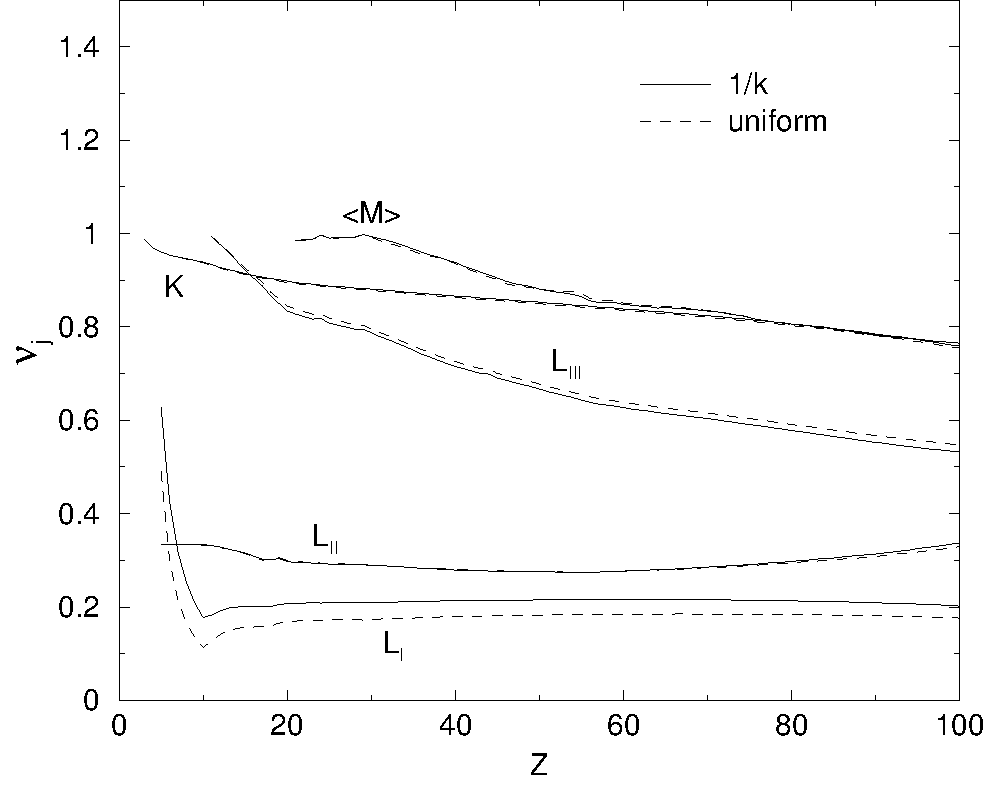
\includegraphics[height=12cm,width=12cm]{figures/intp}
\caption[Interaction probabilities for different shells]{\label{phot_intp}
Interaction probabilities $\nu_j$ for different shells as
calculated from Eq. (\protect\ref{photo_nuj}) using
$\phi(k)=1/k$ (solid lines) or $\phi(k)=\mbox{const}$ (dashed lines).}
\end{figure}
Figure \ref{phot_intp} shows the interaction probabilities
$\nu_j$ of the $K, L_I, L_{II}$ and  $L_{III}$ shells and an
``average'' $M$ shell (see next paragraph)
as a function of the
atomic number $Z$ for $\phi(k) = \mbox{const}$ (dashed line)
and $\phi(k) = \mbox{const}/k$ (solid line).
Shell-wise photo-absorption cross section from
the Evaluated Photon Data Library (EPDL) \cite{Cu89}
were used to generate this figure, the upper limit of
the $k$-integration was set to 1 MeV. The dependence of
the $\nu_j$s on the weighting function $\phi(k)$ is
negligible except for the $L_I$ shell where the difference
is of the order of 10\%. This fact was the motivation for
using the energy independent interaction probabilities $\nu_j$,
a better approach is scheduled for a future release of the
system.

The use of an interaction probability for an ``average'' $M$-shell
is motivated by the fact that relaxation transitions from and to
$M$-shells are treated in an average way, see section \ref{relax}.
Given the definition of the $\nu_j$'s, $\nu_{\langle M \rangle}$ is
\begin{equation}
\nu_{\langle M \rangle} = 1 - \prod (1 - \nu_{M_i})
\end{equation}
where the product runs over the number of $M$-sub-shells available
for the element $Z$ (up to 5). The interaction probabilities
$\nu_K, \nu_{L_I}, \nu_{L_{II}}, \nu_{L_{III}}$ and $\nu_{\langle M \rangle}$,
calculated with the $1/k$ weighting function, are stored in the
file {\tt photo\_relax.data} and read in by the subroutine
{\tt edgset} which is called from {\tt HATCH}.

With all this, the algorithm for selecting the shell that absorbs
the incident photon is as follows:
\begin{itemize}
\item[2.1]
Determine the inner-most shell $j$ that has a binding energy lower
than the incident photon energy and pick a random number $r_2$
\item[2.2]
If $r_2 < \nu_j$ or $j > \langle M \rangle$
\footnote{The outer-most shell treated is the $M$ shell, if the photon
was not absorbed by it, it is assumed that it is absorbed by the
$N$ shell.}, then deliver $j$
\item[2.3]
Set $r_2 = (1 - r_2)/(1 - \nu_j),~j = j+1$, go to step 2.2
\end{itemize}
\item
Once the element and its shell absorbing the photon is determined,
a photo-electron with the kinetic energy $k - U_j(Z)$ is set-up, where
$U_j(Z)$ is the binding energy of the selected shell.
The vacancy created is treated in the routine ({\tt relax}, see section
\ref{relax}),
this significant change compared to EGS4 is motivated by the
fact that shell vacancies are created also
in other processes, {\em e.g.} Compton scattering (see section \ref{compton}).
The sampling of the photo-electron direction is discussed in section
\ref{photo_direction}.
\end{enumerate}

\paragraph{Simplified simulation of photo-electric absorption}\hfill
\label{photo_simple}
\index{photo-electric absorption!simplified simulation of}

If the flag {\tt IEDGFL} for the current region is set to zero,
a simplified simulation of the photo-absorption process is undertaken.
This simplified treatment consists of one step:
\index{IEDGFL}
\begin{enumerate}
\item
Set-up a photo-electron with a kinetic energy $k$
\end{enumerate}
There are several reasons which motivated us to change the
logic compared to the current EGS4 version (where the
$K$-shell binding energy is always subtracted):
\begin{itemize}
\item
The treatment is greatly simplified
\item
If the flag {\tt IEDGFL} is set to zero, it is reasonable to assume
that the detailed calculation of the spread of energy released
in photo-absorption events is not important for the situation
under investigation
\item
The effect of the production of relaxation particles in the
de-excitation cascade following photo-electric absorption is
to spread out the binding energy around the point of interaction.
By giving the photo-electron the entire incident photon energy,
this effect is at least partially simulated.
\end{itemize}

\paragraph{Photo-electron direction}\hfill
\label{photo_direction}
\index{photo-electric absorption!direction of electron}

\index{IPHTER}
The behavior of the sampling of the photo-electron direction
is controlled by the switch {\tt IPHTER}
(included in the {\tt COMIN/EDGE} common block) which set on a
region by region basis. If set to zero,
the photo-electron ``inherits'' the direction of the incident
photon. If set to non-zero (the default selection),
the direction is sampled from the
Sauter distribution \cite{Sa31}. The implementation as discussed
in detail in Ref. \cite{BR86a} is adopted. For completeness, we give a
brief summary here.
\index{Bielajew, Alex}

Sauter's distribution in the polar angle
$\mu = \cos \theta$ with respect to the incident
photon direction may be cast in the form \cite{BR86a}
\begin{equation}
f(\mu) {\rm d}\mu = {1 - \mu^2 \over (1 - \beta \mu)^4} \left[ 1 +
\kappa (1 - \beta \mu) \right] {\rm d} \mu
\end{equation}
where $\beta$ is the electron's velocity in units of the
speed of light  and
\begin{equation}
\kappa = {\gamma \over 2} (\gamma - 1) (\gamma - 2)~, \quad \gamma =
{1 \over \sqrt{1 - \beta^2} }
\end{equation}
This equation can be sampled by generating candidate
$\mu$ values from
\begin{equation}
g(\mu) = {1 \over 2 \gamma^2 (\kappa + \gamma)^2} ~{
1 + \kappa (1 - \beta \mu) \over (1 - \beta \mu)^2 }~,
\end{equation}
which is a normalized PDF for $\mu$, and using
\begin{equation}
h(\mu) = { \gamma + 1 \over 2 \gamma } ~{1 - \mu^2 \over 1 - \beta \mu }
\end{equation}
which is always positive and has a maximum of unity,
as a rejection function. To generate $\mu$ values from
$g(\mu)$, one uses
\begin{equation}
\mu = {1 \over \beta} \left[1 - \left( \sqrt{\left(\kappa + {1 \over 1 + \beta}
\right)^2 + 4 \beta \gamma^2 (\kappa + \gamma^2) r_1} - \kappa \right)^{-1}
\right]
\end{equation}
where $r_1$ is an uniformly distributed random number.

\index{Sauter distribution}
It is worth noticing that, strictly speaking, Sauter's distribution is
valid only for the $K$-shell and also derived
from an extreme relativistic approximation. The treatment
of the photo-electron angular distribution is therefore left
as a macro {\tt \$SELECT-PHOTOELECTRON-DIRECTION;}
and can therefore be replaced, if the user has a better approach.
\index{\$SELECT-PHOTOELECTRON-DIRECTION}

\subsubsection{Coherent (Rayleigh) scattering}
\label{rayleigh}
\setcounter{equation}{0}
\index{Rayleigh scattering}
\index{coherent scattering}
\index{cross section!coherent}

Originally, EGSnrc ``inherited'' the treatment of the coherent
photon scattering process from EGS4 \cite{Ne85}.
This means that the total coherent scattering cross
sections from Storm and Israel \cite{SI70} and the atomic
form factors $F_T(q,Z)$ from Hubbel and {\O}verb{\o} \cite{HO79} are used
by default.
The form factors for molecules are calculated from the independent
atom approximation, {\em i.e.}
\begin{equation}
[F_T(q)]^2 = \sum p_i [F_T(q,Z_i)]^2
\end{equation}
where $p_i$ is the stoichiometric index of the $i$'th element,
$Z_i$ its atomic number and $q$ the momentum transfer when
a photon with an energy $k$ is scattered by an angle $\theta$,
\begin{equation}
q = k \sqrt{{1 - \cos \theta \over 2}}~.
\end{equation}
The coherent scattering cross section, differential in the
photon angle $\Omega = (\theta, \phi)$ is
\begin{equation}
{{\rm d} \sigma_{\rm R} \over {\rm d} \Omega} = {r_0^2 \over 2}
(1 + \cos^2 \theta) [F_T(q)]^2~.
\end{equation}
This equation is sampled by re-writing it in terms of
$q^2$,
\begin{equation}
{{\rm d} \sigma_{\rm R} \over {\rm d} q^2} = {4 \pi r_0^2 \over k^2}~
A(q_{\rm max}^2)~
{1 + \cos^2 \theta \over 2} ~{[F_T(q)]^2 \over A(q_{\rm max}^2)
}
\end{equation}
where
\begin{equation}
A(q^2) = \int\limits_0^{q^2} {\rm d}q^{'2} [F_T(q')]^2
\end{equation}
and $q_{\rm max} = k$ is the maximum possible momentum transfer, and
using $[F_T(q)]^2/A(q_{\rm max}^2)$  as a PDF for $q^2$ and
$(1 + \cos^2 \theta)/2$ as a rejection function.

\index{coherent scattering!sampling of}
\index{IRAYLR}  \index{\$RAYLEIGH-SCATTERING;}
The actual sampling, accomplished in the macro
{\tt \$RAYLEIGH-SCATTERING;}, is performed only
if the switch {\tt IRAYLR} (included
in the {\tt COMIN/MISC} common block--see Section~\ref{common_blocks})
is set to non-zero for the current
region. By default, {\tt IRAYLR} is set to zero in the {\tt
block data} subprogram. The motivation for this choice is
the fact that the {\tt \$RAYLEIGH-SCATTERING;} macro
requires the function $A(q^2)$ to be included in the PEGS data
set. This additional data is only included, if the user specifically
requested it from PEGS.

We recommend the Rayleigh
scattering option to be used for low energy calculations
(say, below 1 MeV). It is worth noticing that
inclusion of coherent scattering without the use
of the bound Compton scattering option (see section \ref{compton})
results in too much photon scattering, binding effects
for incoherent scattering should therefore always be turned
on if the Rayleigh option is used.

\paragraph{New coherent scattering angular sampling}\hfill
\label{new_rayleigh_sampling}

\index{Rayleigh scattering!new angular sampling}
% The above sampling algorithm approximates the angular distribution
% for coherent scatter relatively well. However,
% the forward peaked shape of $[F_T(q)]^2/A(q_{\rm max}^2)$
% and its uniform sampling in equidistant intervals
% between 0 and 1 translates into a non-uniform sampling
% of the scattering angle since larger angular intervals
% are covered with increasing bin number. As a consequence,
The original EGS4 sampling algorithm produces a step-like averaging
artifact at large angles, which increases with energy. This is
shown by the symbols in Figure \ref{ray_ang_sampling_fig}, for
20 keV, 60 keV and 110 keV photon beams in water.
However, this artifact has no practical consequences, unless one is
interested in the few photons scattered at large angles.
\begin{figure}[h]
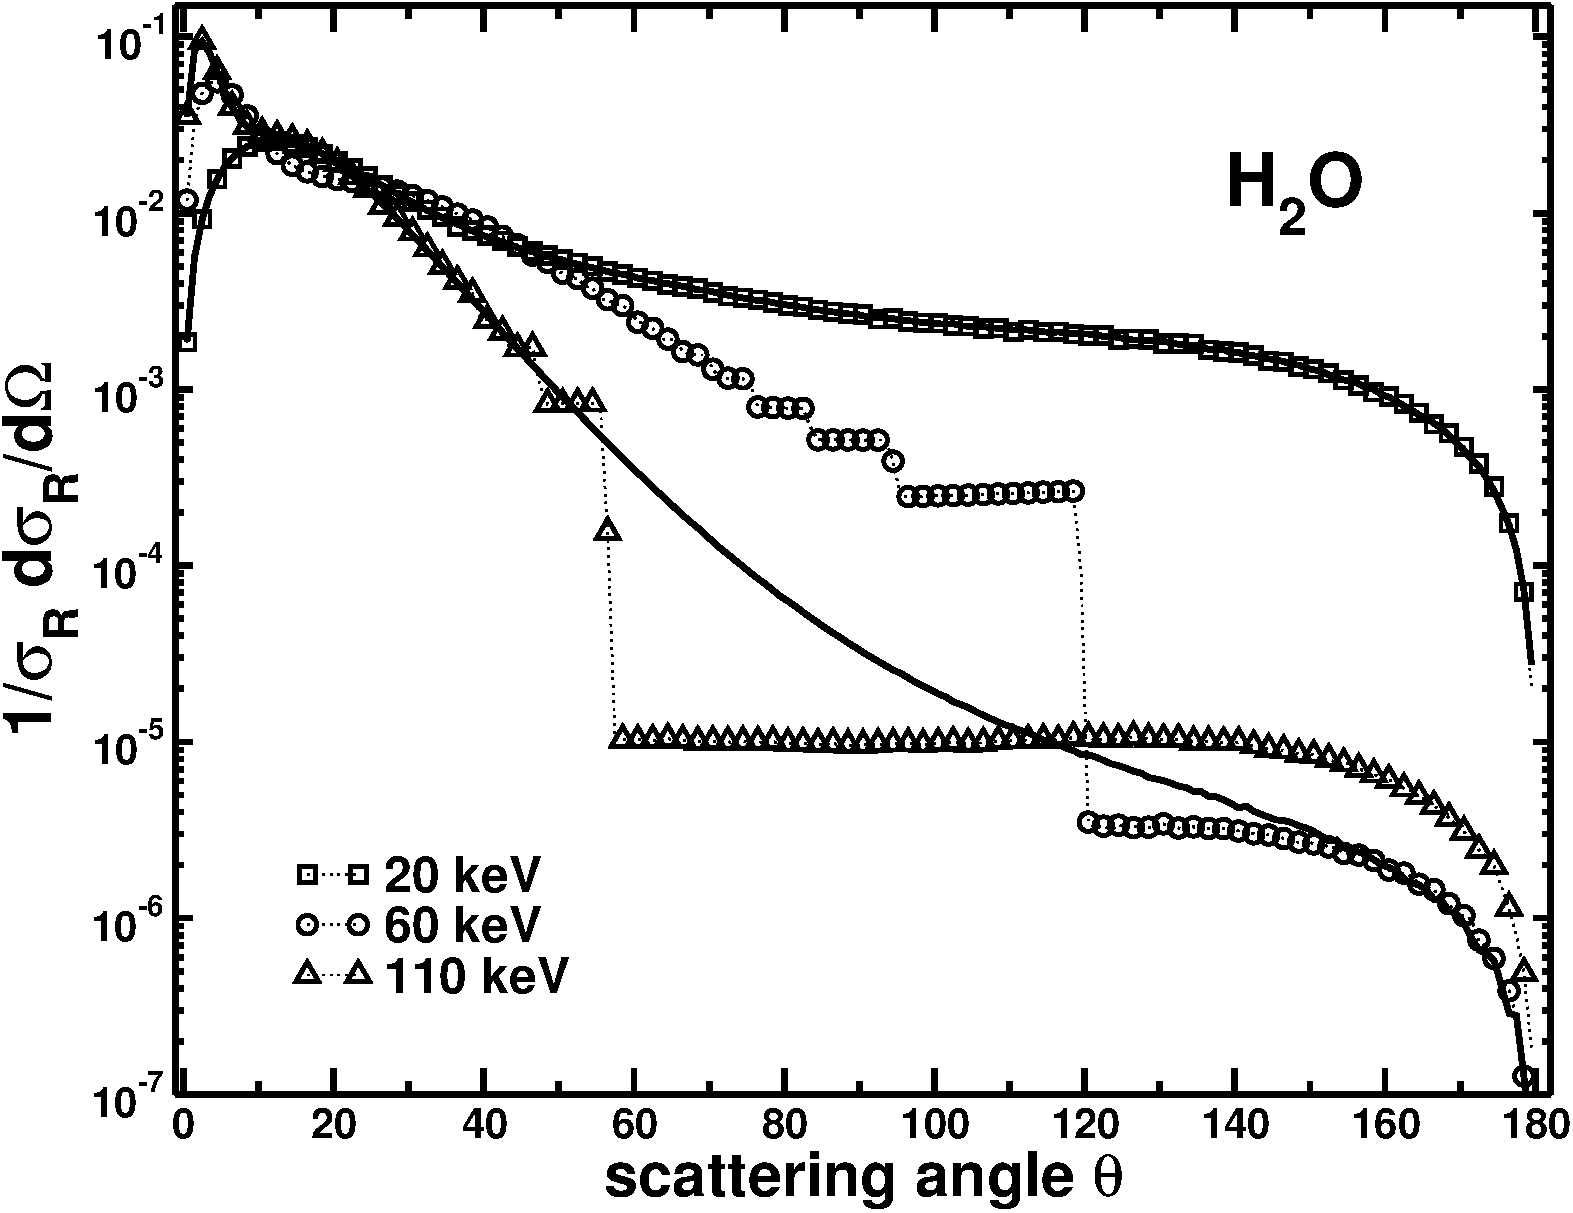
\includegraphics[height=9cm,width=9cm]{figures/ray_ang_dist_old_vs_new}
\caption[Angular distribution of coherently scattered photons for 20 keV, 60 keV
and 110 keV photon beams in water.]{\label{ray_ang_sampling_fig}
Angular distribution of coherently scattered photons for 20 keV, 60 keV
and 110 keV photon beams in water. Symbols represent the original EGS4
sampling algorithm and the solid lines the new alias sampling.
}
\end{figure}

The default angular sampling algorithm for coherent scattering
was replaced in 2007 for an alias-sampling algorithm that properly
samples $[F_T(q)]^2/A(q_{\rm max}^2)$ removing this artifact as shown
by the solid lines in Figure \ref{ray_ang_sampling_fig} for 20 keV
and 110 keV. The coherent scattering form factors are now
read directly either from {\tt \$HEN\_HOUSE/pegs4/pgs4form.dat}
(default atomic form factors, see section \ref{rayleigh} above) or from
user-supplied form factor files expected to be in the
{\tt \$HEN\_HOUSE/data/molecular\_form\_factors/} directory
(see section \ref{custom_ff_sect} below for more details).
This means that one can now switch on coherent (Rayleigh) scattering,
even if there is no Rayleigh data in the PEGS4 data set.

The old sampling macro is now named {\tt \$OLD\_RAYLEIGH-SCATTERING;}.
If one is interested
in reproducing old calculations or just want to use the old sampling,
this macro could be renamed back to {\tt \$RAYLEIGH-SCATTERING;}.
Please note that in this case a PEGS4 file is required with the needed
interpolation coefficients and the input key {\tt Photon cross sections}
in the {\tt MC transport parameters input block} must be set to {\tt PEGS4}
(see section \ref{xsections}, page~\pageref{xsections}).

\paragraph{Custom atomic and molecular form factors}\hfill
\label{custom_ff_sect}
\index{Rayleigh scattering!custom form factors}

\index{iray\_ff\_file}\index{iray\_ff\_media}
The user now has the option of supplying their own custom atomic
or molecular form factors for determining Rayleigh cross sections.
These are specified through the {\tt iray\_ff\_media} (medium names) and
{\tt iray\_ff\_file} (files containing form factor data)
variables contained in the
{\tt COMIN/RAYLEIGH\_INPUTS} common block.
\index{RAYLEIGH\_INPUTS common block}
A number of measured molecular form factors from the work by
Peplow and Verghese \cite{PV98} are distributed with EGSnrc and can be
found in the {\tt \$HEN\_HOUSE/data/molecular\_form\_factors} directory.

To enable this option, one needs to set the input key {\tt Rayleigh scattering}
to {\tt custom} in the {\tt MC transport parameters} input block. An example
of such an input is shown below:

\begin{verbatim}
:start MC transport parameter:
  .
  .
  .
  Rayleigh scattering=  custom
  ff media names = BREASTICRU512 \
                   FATICRU512 \
                   MUSCLEICRU512 \
                   KAPTONICRU512
  ff file names = /ff_file_location/mff_breast_tissue.dat \
                  /ff_file_location/mff_pork_fat.dat \
                  /ff_file_location/mff_pork_muscle.dat \
                  /ff_file_location/mff_kapton.dat

:stop MC transport parameter:
\end{verbatim}

Note that since there is no check, the user must make sure that the medium name and
the form factor file correspond to the same material.

\subsubsection{Changing photon cross sections}
\label{photon_xsect}
\index{photon cross section data!changing}
\index{photon\_xsections}
\index{XCOM}
\index{EPDL}
\index{Storm \& Israel}

In the current version of EGSnrc, the user has the option to use
photon cross section data other than the default
Storm \& Israel data.  To do this, the user must
set the character variable {\tt photon\_xsections} (part of the
{\tt COMIN/MEDIA} common block) to the name of the cross section
data to use.  Cross sections included with the EGSnrc distribution
are: 1) the Evaluated Photon Data
Library\cite{Cu97a} (set {\tt photon\_xsections= "epdl"})
2) XCOM data from Berger \& Hubbell\cite{BH87} (set {\tt photon\_xsections= "xcom"}
-- also the default in the absence of any input)
and 3) Storm \& Israel\cite{SI70} (set {\tt photon\_xsections= "si"}). For information on how
to set the variable {\tt photon\_xsections}, the reader
is referred to section~\ref{step_2} (page~\pageref{photon_xsections_description}).

The user can also supply their own photon cross section data.
This can be accomplished by placing data files named
{\tt xxxx\_photo.data, xxxx\_pair.data, xxxx\_triplet.data} and {\tt xxxx\_rayleigh.data}
in the {\tt \$HEN\_HOUSE/data} folder, where {\tt xxxx} stands for any string different
from {\tt epdl, xcom} or {\tt si}. These cross sections will then be used if
the variable {\tt photon\_xsections} is set to {\tt xxxx}. The format of the
ASCII data files is very simple: for each element between 1 and 100 one has to
provide the number $N$ of data points in the tabulation followed by $N$
pairs of the logarithm of the photon energy in MeV and the logarithm of the
cross section in barn (see also one of the data files provided with EGSnrc).

Since 2006 EGSnrc was modified to ignore the photon data in the PEGS4
file, re-initializing all interpolation tables to utilize the
maximum number of interpolation bins availble. In this way, the user
can minimize the inaccuracies around atomic edges by replacing \$MXGE with
a huge number in their user code. Starting with the 2011 release
(V4 release 2.3.2), the use of PEGS4 photon data has been re-enabled for
backwards compatibility.
To achieve this, the user must set the character variable
{\tt photon\_xsections} to {\tt PEGS4} (case insensitive). See
section \ref{xsections} (page~\pageref{xsections}) for more
information on this topic.

It is worth noting that the total cross section for Compton scattering is
normally obtained from the theoretical differential cross section being used
(Klein-Nishina or RIA, see section \ref{compton}) by
integrating over the kinematically allowed range instead of being taken from
tabulations. This behavior can be changed by the user as described in
section \ref{compton}).

\subsection{Atomic Relaxations}
\label{relax}
\index{atomic relaxations}
\index{relaxations}
\index{fluorescent X-rays}
\index{Auger transitions}
\index{Coster-Kronig transitions}

Excited ions, produced by the interaction of photons and
charged particles when they travel through matter, relax to
their ground state by migration of the initial vacancy to
outer shells via the emission of characteristic X-rays and/or
Auger or Coster-Kronig electrons (see {\em e.g.} Ref. \cite{Pe91}).

In the current standard version of EGS4, only $K$-shell relaxations following
photo-electric absorption via
the emission of $K_\alpha$ and $K_\beta$ fluorescence are treated
and are intrinsically associated with the {\tt PHOTO} routine.
An extension to include $L$-shell fluorescence was developed by the
KEK group \cite{Na98} and is available for use with the EGS4 system.

In EGSnrc we have extended the treatment of atomic relaxations
to include higher shells as well as the production of Auger and
Coster-Kronig electrons. With these extensions, the
treatment within the {\tt PHOTO} routine
has become unpractical. In addition, the relaxation cascade
is a separate process, it can be initiated after any photon
or electron interaction that has produced an inner shell vacancy.
The most general approach for treating excited atoms or ions would have
been to define a separate particle type, an excited atom or ion, and to
put such particles on the stack whenever they are produced.
Such an approach would have been too a large departure from
the EGS4 logic and potentially render many user codes unusable.
We have therefore abandoned this idea and decided to
treat relaxations in a separate routine ({\tt relax}),
which is called whenever an inner shell vacancy is created.
In this release of EGSnrc, such vacancies can be created in
photo-absorption events (see section \ref{photo}) and in
Compton scattering events (see section \ref{compton}).
It is anticipated that the next release of the system
will include the explicit modeling of inner shell
ionizations by electron or positron impact.

\index{low energy limit!photon}
\index{energy range}
\index{limitations!energy}
The de-excitation cascade is a complex process, there are
hundreds of possible transitions for high-$Z$ elements.
A complete treatment goes beyond the scope of a general
purpose code for the simulation of electron and photon transport
such as EGSnrc. In addition, we consider 1 keV to be the lowest
limit for the applicability of the code. We have therefore imposed
a lower limit of 1 keV on the relaxation process, {\em i.e.} only
vacancies in shells with binding energies
above 1 keV are treated.\footnote{Another motivation
for imposing this limit is the fact that uncertainties on
transition probabilities rapidly increase with
decreasing binding energies, they are perhaps 10 or 20\%
even for $L$-shells} If we then take into account that
only elements with $Z \ge 52$ have $M$-shells with binding energies
above the limit of 1 keV and that $M$-shells have binding energies less
than 10 keV for all elements (the $M_I$ binding energy for
lead is 3.8 keV and 7.2 keV for Einsteinium \cite{Pe91}),
it is a reasonable approach to model transitions from and
transitions to $M$-shells in an ``average'' way.
There is of course no unique procedure to set the binding energies of the
``average'' $M$-shells for the elements, $U_{\langle M \rangle}(Z)$,
to be used in the de-excitation cascade.
Assuming that for most applications $K$ to $M$ transitions
are more important than $L$ to $M$ or $M$ to a lower shell,
we have defined $U_{\langle M \rangle}(Z)$ to be the weighted average
of the binding energies $U_{M_j}(Z)$ of the element $Z$ with
weights given by the $K$ to $M_j$ transition probabilities $\nu_{KM_j}$,
\begin{equation}
U_{\langle M \rangle}(Z) \equiv {\sum \nu_{KM_j} U_{M_j} \over
\sum \nu_{KM_j}}
\end{equation}
For instance, $U_{\langle M \rangle}$ determined by this
procedure using transition probabilities from the
Evaluated Atom Data Library (EADL) \cite{Pe91} for lead
is 3.1 keV, the $M_I$ binding energy is 3.8 keV and the
$M_V$ binding energy 2.5 keV. A simple averaging with the
occupation numbers would result in an average $M$-shell binding
energy of 2.9 keV. If distinguishing between any of the above
numbers is important for your application, EGSnrc is most
likely not the most appropriate simulation package for
your purposes.
\index{limitations!M shell}

Having said all this, it is apparent that $N$ shells are
also treated in an average way. The only elements with
``average'' $N$-shell binding energies above 1 keV are those with $Z > 95$.

In an implementation consistent with the overall logic
of the EGS system, the relaxation algorithm should
put all particles produced in the course of the
de-excitation cascade on the particle stack, they would
then be discarded in the {\tt PHOTON} or {\tt ELECTR}
routines if their energies were below the specified
transport threshold energies. It is easy to see that
such an approach may become extremely wasteful if
the transport threshold energies are large compared to
the lower limit of 1 keV for the de-excitation cascade.
We have therefore decided to stop the relaxation process
for vacancies with binding energies less then $E_{\rm min}$,
\begin{equation}
E_{\rm min} = \mbox{Max} \{ 1~\mbox{keV},~\mbox{Min}
\{ {\tt PCUT}, {\tt ECUT} - m \} \}
\end{equation}
and to score their energy locally. In addition,
the energy of photons or electrons that are below
the thresholds are also deposited locally, even if
they were produced in transitions from vacancies
with binding energies above $E_{\rm min}$.
The total sub-threshold energy is collected in
the variable {\tt EDEP}, which is in the {\tt COMON/EPCONT/},
and made known to the
user via an {\tt IARG=4} call to the scoring routine.
\index{IARG!4}
\index{EDEP}

To facilitate the handling of the relaxation cascade, we
define a shell number $n$ for each of the shells treated.
$K$-shells have $n=1$, $L_I$ through $L_{III}$ have $n=2$ to 4,
$\langle M \rangle$ corresponds to $n=5$, $\langle N \rangle$ to
$n=6$, all other shells have $n=7$. A list of possible
transitions, $L_n$, is associated with each shell,
\begin{equation}
L_n = \{ (\nu_1, s_1), (\nu_2, s_2), \cdots, (\nu_{k_n}, s_{k_n}) \}
\end{equation}
where $k_n$ is the number of possible transitions for the shell
of type $n$ and $\nu_i$ the transition probabilities for
a transition into final state $s_i$.  The final states
$s_i$ are defined as follows:
\begin{equation}
s_i =
\left\{
\begin{array}{l@{\quad , \quad}l}
n_i & \mbox{for fluorescent transitions} \\
10 + n_i & \mbox{for Coster-Kronig transitions} \\
100 n_{i,1} + n_{i,2} & \mbox{for Auger transitions}
\end{array}
\right.
\end{equation}
where $n_i$ or $n_{i,1}$ and $n_{i,2}$ are the shell numbers of the
new vacancies created in fluorescent and Coster-Kronig or Auger transitions.
Table \ref{relax_transitions}
summarizes all transitions handled in the current version
of the relaxation routine.
\index{relaxation transitions}
%\begin{longtable}[htb]
\begin{table}[phtb]
\caption{\label{relax_transitions} Relaxation transitions handled
by EGSnrc.}
%\hline \hline
%initial vacancy & shell code & transition & final state code \\
%\hline \hline
%\endhead
%\hline \hline
%\endfoot
\begin{center}
\begin{tabular}{|c|c|c|c|}
\hline \hline
initial vacancy & shell code & transition & final state code \\
\hline \hline
 & & Fluorescent $K \to L_{II}$ & \phantom{00}3 \\
 & & \phantom{Fluorescent} $K \to L_{III}$ & \phantom{00}4 \\
 & & \phantom{Fluorescent} $K \to \langle M \rangle$ & \phantom{00}5 \\
 & & \phantom{Fluorescent} $K \to \langle N \rangle$ & \phantom{00}6 \\
 & & Auger $K \to L_I L_I$ & 202 \\
 & & \phantom{Auger} $K \to L_{II} L_{I}$ & 302 \\
 & & \phantom{Auger} $K \to L_{II} L_{II}$ & 303 \\
 & & \phantom{Auger} $K \to L_{III} L_{I}$ & 402 \\
 & & \phantom{Auger} $K \to L_{III} L_{II}$ & 403 \\
 $K$ & 1 & \phantom{Auger} $K \to L_{III} L_{III}$ & 404 \\
 & & \phantom{Auger} $K \to \langle M \rangle L_{I}$ & 502 \\
 & & \phantom{Auger} $K \to \langle M \rangle L_{II}$ & 503 \\
 & & \phantom{Auger} $K \to \langle M \rangle L_{III}$ & 504 \\
 & & \phantom{Auger} $K \to \langle M \rangle \langle M \rangle $ & 505 \\
 & & \phantom{Auger} $K \to \langle N \rangle L_{I}$ & 602 \\
 & & \phantom{Auger} $K \to \langle N \rangle L_{II}$ & 603 \\
 & & \phantom{Auger} $K \to \langle N \rangle L_{III}$ & 604 \\
 & & \phantom{Auger} $K \to \langle N \rangle \langle M \rangle $ & 605 \\
 & & \phantom{Auger} $K \to \langle N \rangle \langle N \rangle $ & 606 \\
\hline
& & Fluorescent $L_I \to \langle M \rangle$ & \phantom{00}5 \\
& & \phantom{Fluorescent} $L_I \to \langle N \rangle$ & \phantom{00}5 \\
& & Coster-Kronig $L_I \to L_{II}$ & \phantom{0}13 \\
$L_I$ & 2 & \phantom{Coster-Kronig} $L_I \to L_{III}$ & \phantom{0}14 \\
& & Auger $L_I \to \langle M \rangle \langle M \rangle$ & 505 \\
& & \phantom{Auger} $L_I \to \langle N \rangle \langle M \rangle$ & 605 \\
& & \phantom{Auger} $L_I \to \langle N \rangle \langle N \rangle$ & 606 \\
\hline
& & Fluorescent $L_{II} \to \langle M \rangle$ & \phantom{00}5 \\
& & \phantom{Fluorescent} $L_{II} \to \langle N \rangle$ & \phantom{00}6 \\
& & Coster-Kronig $L_{II} \to L_{III} $ & \phantom{0}14 \\
$L_{II}$ & 3 & Auger $L_{II} \to \langle M \rangle \langle M \rangle$ & 505 \\
& & \phantom{Auger} $L_{II} \to \langle N \rangle \langle M \rangle$ & 605 \\
& & \phantom{Auger} $L_{II} \to \langle N \rangle \langle N \rangle$ & 606 \\
\hline
& & Fluorescent $L_{III} \to \langle M \rangle$ & \phantom{00}5 \\
& & \phantom{Fluorescent} $L_{III} \to \langle N \rangle$ & \phantom{00}6 \\
$L_{III}$ & 4 & Auger $L_{III} \to \langle M \rangle \langle M \rangle$ & 505 \\
& & \phantom{Auger} $L_{III} \to \langle N \rangle \langle M \rangle$ & 605 \\
& & \phantom{Auger} $L_{III} \to \langle N \rangle \langle N \rangle$ & 606 \\
\hline
$\langle M \rangle$ & 5 & Fluorescent
$\langle M \rangle \to \langle N \rangle$  & 6 \\
& & Auger $\langle M \rangle \to \langle N \rangle
\langle N \rangle$ & 606 \\
\hline \hline
\end{tabular}
\end{center}
\end{table}

In addition, we define a ``vacancy stack'' which holds all vacancies
at a given stage of the relaxation cascade.

\index{relaxations!simulation of}
\index{atomic relaxations!simulation of}
With these definitions in place, the simulation of the relaxations
cascade becomes fairly simple:
\begin{enumerate}
\item
Put the initial vacancy in the ``vacancy stack'', set the ``vacancy stack''
counter $m$ to 1
\item
If $m=0$, return control to the calling routine
\item
Take the top vacancy, to be denoted by $n_i$ in the following,
from the ``vacancy stack'', reduce $m$ by 1
\item
If $U_{n_i} < E_{\rm min}$, then ${\tt EDEP = EDEP} + U_{n_i}$, go to
step 2
\item
Pick a random number $r$, set $j = 1$
\item
If $r \le \nu_j$, go to step 8
\item
$r = (1 - r)/(1 - \nu_j),~~j = j+1$,~go to step 6
\item
$j$ is the number of the selected transition,
\begin{itemize}
\item[8.1]
if $s_j < 10$, then the new vacancy is in shell $n_j = s_j$, put
it on the ``vacancy stack'', increase $m$ by one, produce a
fluorescent photon with
energy $E = U_{n_i} - U_{n_j}$. If $E < {\tt PCUT}$, then
${\tt EDEP = EDEP} + E$, else, select the photon direction uniformly and
put it on the EGSnrc particle stack
\item[8.2]
else if $s_j < 100$, then the new vacancy is in shell $n_j = s_j - 10$,
put it on the ``vacancy stack'', increase $m$ by one, produce a
Coster-Kronig electron with kinetic
energy $E = U_{n_i} - U_{n_j}$. If $E < {\tt ECUT} - m$, then
${\tt EDEP = EDEP} + E$, else, select the electron direction uniformly
and put it on the EGSnrc particle stack
\item[8.3]
else, the two new vacancies are $n_{j,1} = (s_j~\mbox{mod}~100)$ and
$n_{j,2} = s_j - 100~ n_{j,1}$, put them on the ``vacancy stack'',
increase $m$ by two,
produce an Auger electron with a kinetic energy
$E = U_{n_i} - U_{n_{j,1}} - U_{n_{j,2}}$.
If $E < {\tt ECUT} - m$, then
${\tt EDEP = EDEP} + E$, else, select the electron direction uniformly
and put it on the EGSnrc particle stack
\end{itemize}
\item
Go to step 2
\end{enumerate}
Finally, we have defined for each of the steps 8.1 to 8.3 new calls to
the routine {\tt AUSGAB} with arguments {\tt IARG} = 25 to 27.
This gives the possibility for the user to take some actions
with the relaxation particles, {\em e.g.}, set their {\tt LATCH} variable
to an appropriate value, or play Russian Roulette with them.
\index{AUSGAB}
\index{IARG!25,26,27:}
%\clearpage


%%%%%%%%%%%%%%%%%%%%%%%%%%%%%%%%%%%%%%%%%%%%%%%%%%%%%%%%%%%%%%%%%%%%%%%%%%%%%%%
%
%  EGSnrc manual: electron transport
%  Copyright (C) 2015 National Research Council Canada
%
%  This file is part of EGSnrc.
%
%  EGSnrc is free software: you can redistribute it and/or modify it under
%  the terms of the GNU Affero General Public License as published by the
%  Free Software Foundation, either version 3 of the License, or (at your
%  option) any later version.
%
%  EGSnrc is distributed in the hope that it will be useful, but WITHOUT ANY
%  WARRANTY; without even the implied warranty of MERCHANTABILITY or FITNESS
%  FOR A PARTICULAR PURPOSE.  See the GNU Affero General Public License for
%  more details.
%
%  You should have received a copy of the GNU Affero General Public License
%  along with EGSnrc. If not, see <http://www.gnu.org/licenses/>.
%
%%%%%%%%%%%%%%%%%%%%%%%%%%%%%%%%%%%%%%%%%%%%%%%%%%%%%%%%%%%%%%%%%%%%%%%%%%%%%%%
%
%  Author:          Iwan Kawrakow, 2003
%
%  Contributors:    Blake Walters
%                   Ernesto Mainegra-Hing
%                   Frederic Tessier
%
%%%%%%%%%%%%%%%%%%%%%%%%%%%%%%%%%%%%%%%%%%%%%%%%%%%%%%%%%%%%%%%%%%%%%%%%%%%%%%%


\subsection{Simulation of electron transport}
% Replace commented line for the one with fixed date when commiting
% Beware: Using the macro below conflicts between CVS and latex!!!
% \lfoot[{\sffamily {\leftmark}}]{{\small Last edited $Date: 2014/09/08 23:08:01 $
\lfoot[{\sffamily {\leftmark}}]{{\small Last edited 2011/05/02 18:42:31
}}

\label{chapter_electron_transport}
\index{electron transport}
\index{condensed history technique}
\index{Class II scheme}

%\subsection{Simulation of electron transport}
\subsubsection{General discussion}
\label{electron_general}
\setcounter{equation}{0}
\index{electron transport!general discussion}

The Condensed History (CH) Technique was introduced by M. Berger in
the early sixties \cite{Be63}.
In this technique, many track segments of the real electron random
walk are grouped into a single ``step''. The cumulative effect
of elastic and inelastic collisions during the step are taken into
account by sampling energy and direction changes from
appropriate multiple scattering distributions at the end of the step.
This approach is justified by the observation that the changes of
the electron state in a single collision are usually very small and
fails when this condition is not satisfied (at very low energies).
Berger also defined two different implementations of the CH technique,
which he called Class I and Class II schemes.
\index{Class I scheme}
\index{Class II scheme}

EGSnrc uses a Class II CH scheme
for the simulation of electron transport.
That is to say, bremsstrahlung processes that result in the
creation of photons above an energy threshold $k_c$, and
inelastic collisions that set in motion atomic electrons with
kinetic energies above $T_c$, are both simulated explicitly and the
secondaries transported. Such interactions are also referred to as
``catastrophic'' collisions.
Sub-threshold inelastic and radiative events and
elastic collisions are subject to grouping.
\index{catastrophic collisions}
\index{discrete interactions}

Every CH scheme must provide rules for selecting
a path-length $\Delta s_n$, an energy loss $\Delta E_n$,
a change in direction from
$\Omega_n$ to $\Omega_{n+1}$ and a spatial displacement
$\Delta \vec{x}_n$ for each step of the CH random walk. For transport in
heterogeneous geometries a boundary crossing algorithm is
also required.

In the following we give a brief transport-theoretical
treatment of a Class II CH technique which will help
to establish the motivation and definitions of
various quantities used in the CH implementation.

\index{transport equation}
The transport equation for the electron fluence
$\Phi(\vec{x},\vec{\Omega},E,t)$ in a medium with a density of
scattering centres (atoms or molecules) $n(\vec{x})$ is given by
\begin{equation}
\label{transport1}
{{\rm d}\Phi(\vec{x},\vec{\Omega},E,t) \over {\rm d}t} =
\index{electron transport!general discussion}
S(\vec{x},\vec{\Omega},E,t) + v I[\Phi]
\end{equation}
where
\begin{itemize}
\item
$S(\vec{x},\vec{\Omega},E,t)$ is the number of electrons with energy
$E$ and velocity $\vec{v} = (v,\vec{\Omega})$ at a position $\vec{x}$ per unit
volume, energy and solid angle interval, imparted per unit time
by an external source or
by photons interacting with the medium at time $t$. This latter part of the
source term causes the coupling of the electron and photon fluences.
\item
${\rm d}\Phi/{\rm d}t$ is the total time derivative, in the absence
of external force fields it is given by
\begin{equation}
{{\rm d}\Phi(\vec{x},\vec{\Omega},E,t) \over {\rm d}t}  =
{\partial \Phi(\vec{x},\vec{\Omega},E,t) \over \partial t} +
\vec{v} \vec{\nabla} \Phi(\vec{x},\vec{\Omega},E,t)~.
\end{equation}
\item
\index{collision integral}
The collision term $I[\Phi]$ represents the changes of the particle
fluence due to collisions with the atoms or molecules of the
surrounding medium,
\begin{equation}
\begin{split}
I[\Phi]  =
 & - n(\vec{x}) \Phi(\vec{x},\vec{\Omega},E,t)
\int\limits_0^E {\rm d} E' \int\limits_{4 \pi} {\rm d} \vec{\Omega}'
\sigma(E,E',\Omega',\vec{x}) \\
& +
n(\vec{x}) \int\limits_E^\infty {\rm d} E' \int\limits_{4 \pi}
{\rm d}\vec{\Omega}'
\Phi(\vec{x},\vec{\Omega}',E',t)
\sigma(E',E'-E,\vec{\Omega}'\cdot \vec{\Omega},\vec{x})
\end{split}
\end{equation}
where
$\sigma(E,E',\Omega,\vec{x})$ is the microscopic cross section
at a position $\vec{x}$ for all possible interactions in which
an electron with energy $E$ loses energy $E'$ and changes its direction
by $\vec{\Omega}$.
\end{itemize}
The collision integral $I[\Phi]$ represents the balance between
particle losses and gains due to interactions described by the
cross section $\sigma(E,E',\Omega,\vec{x})$.
\index{cross section}

In a Monte Carlo simulation the solution of Eq. \eqref{transport1}
is usually obtained via
\begin{equation}
\label{integrate_green_function}
\Phi(\vec{x},\vec{\Omega},E,t) = \int\limits_0^t {\rm d}t_0
\int\limits_E^\infty {\rm d}E_0 \int {\rm d}\vec{x}_0 \int\limits_{4 \pi}
{\rm d}\vec{\Omega}_0~ S(\vec{x}_0,\vec{\Omega}_0,E_0,t_0)
\Phi_0(\vec{x},\vec{\Omega},E,t)
\end{equation}
where $\Phi_0(\vec{x},\vec{\Omega},E,t)$ is a short hand notation
for $\Phi(\vec{x}_0,\vec{\Omega}_0,E_0,t_0;\vec{x},\vec{\Omega},E,t)$
which is the solution of
Eq. \eqref{transport1} for a source
\begin{equation}
S_0 = \delta^{(3)}(\vec{x} - \vec{x}_0) \delta^{(2)} (\vec{\Omega} -
\vec{\Omega}_0) \delta(E-E_0) \delta(t - t_0)
\end{equation}
{\em i.e.} a single particle set in motion at time $t_0$ with
energy $E_0$, direction $\vec{\Omega}_0$ at a position $\vec{x}_0$.
The integration of Eq. (\eqref{integrate_green_function})
is of course performed by a Monte Carlo technique:
\begin{enumerate}
\item
Pick particles from the source $S(\vec{x},\vec{\Omega},E,t)$,
denote their co-ordinates by $E_0, \vec{x_0}, \vec{\Omega_0}, t_0$.
\item
Solve the transport equation for these particles by a Monte Carlo
simulation ({\em i.e.} solve the transport equation for
$\Phi_0$)
\end{enumerate}
Usually the Monte Carlo simulation is initiated by a single
particle from an external source, which is put on a ``particle
stack''. In EGSnrc this is accomplished by a call to the subroutine
{\tt SHOWER}. Then, at each stage of the Monte Carlo simulation,
the source corresponds to all particles currently on the stack.
\index{SHOWER}

\index{macroscopic cross section}
Sometimes it is customary to use the macroscopic cross section $\Sigma$,
\begin{equation}
\Sigma(E,E',\Omega,\vec{x}) = n(\vec{x}) \sigma(E,E',\Omega,\vec{x})
\end{equation}
which, when integrated over $E'$ and $\Omega'$, represents the number of
interactions per unit length for electrons with energy $E$.
The atom or molecule density $n$ is given by
\begin{equation}
n = \rho \frac{N_A}{M_A} = {\rho \over u A}
\end{equation}
where $N_A = 6.022045\times10^{23}$~mol$^-1$ is
Avogadro constant, $M_A$ the molar mass in mol$^{-1}$,
$u = 1.0665655\times10^{-24}$~g is the atomic mass unit
and $A$ the relative atomic or molecular mass. Macroscopic
cross sections $\Sigma$ are thus obtained from microscopic
cross sections $\sigma$ by multiplication with one of
the above factors.

\index{cross section!bremsstrahlung}
\index{cross section!inelastic collisions}
\index{cross section!elastic}
\index{cross section!annihilation}
For electrons, $\sigma$ is the sum of the
bremsstrahlung cross section $\sigma_{\rm brem}$, the cross section
for inelastic collisions with atomic electrons, $\sigma_{\rm inel}$,
and the elastic scattering cross section $\sigma_{\rm el}$:
\begin{equation}
\sigma(E,E',\Omega,\vec{x}) = \sigma_{\rm brem}(E,E',\Omega,\vec{x})
+ \sigma_{\rm inel}(E,E',\Omega,\vec{x}) +
\sigma_{\rm el}(E,\Omega,\vec{x}) \delta(0)
\end{equation}
where Dirac's $\delta$ function expresses the fact that
elastic collisions are zero energy loss events. Positrons
interact in addition via the annihilation process described
by $\sigma_{\rm annih}$, this cross section enters
only the third term of Eq. (\ref{transport1}), however, as annihilation
leads merely to particle loss  (at least when looking just at
the electron fluence, the corresponding ``gain'' term appears
as a source term for the photon fluence).

\index{Class II scheme}
In a Class II CH implementation the collision integral
is divided into two parts $I_>[\Phi_0]$ and $I_<[\Phi_0]$.
The former includes only interactions
with change in energy larger than $T_c$ (inelastic collisions)
or $k_c$ (bremsstrahlung), the latter only
collision with energy change less than
$T_c$ or $k_c$. Elastic interactions,
being a zero energy loss processes, are included in $I_<[\Phi_0]$.
For brevity we will drop the $\vec{x}$ and time dependence of the
various quantities in the following equations.
We have for $I_>[\Phi_0]$
\begin{equation}
\begin{split}
I_>[\Phi_0] & = \int\limits_{E+T_c}^\infty {\rm d}E' \int\limits_{4 \pi}
{\rm d} \vec{\Omega}' \Phi_0(\vec{\Omega}',E')
\Sigma_{\rm inel}(E',E'-E,\vec{\Omega}\cdot\vec{\Omega}') \\
& + \int\limits_{E+k_c}^\infty {\rm d}E' \int\limits_{4 \pi}
{\rm d} \vec{\Omega}' \Phi_0(\vec{\Omega}',E')
\Sigma_{\rm brem}(E',E'-E,\vec{\Omega}\cdot\vec{\Omega}')
\\
& - \Phi_0(\vec{\Omega},E)
\left[ \Sigma_{\rm inel}^{\rm (tot)}(E) + \Sigma_{\rm brem}^{\rm (tot)}(E)
\right]
\end{split}
\end{equation}
where $\Sigma_{\rm inel}^{\rm (tot)}(E)$ and
$\Sigma_{\rm breml}^{\rm (tot)}(E)$ are the total macroscopic
cross sections for ``catastrophic'' inelastic or bremsstrahlung
collisions, respectively:
\index{catastrophic collisions}
\begin{equation}
\Sigma_{\rm inel,brem}^{\rm (tot)}(E) = \int\limits_{T_c,k_c}^E {\rm d} E'
\int\limits_{4 \pi} {\rm d}\vec{\Omega}'
\Sigma_{\rm inel,brem}(E,E',\Omega')~.
\end{equation}
The $I_<[\Phi_0]$ part reads
\begin{equation}
I_<[\Phi_0] = \int\limits_{4 \pi} {\rm d}\vec{\Omega}'
\left[ \Phi_0(\vec{\Omega}',E)
\Sigma_{\rm el}(E,\vec{\Omega}\cdot\vec{\Omega}') -
\Phi_0(\vec{\Omega},E) \Sigma_{\rm el}(E,\Omega') \right] +
I_{\Delta E}[\Phi_0]
\end{equation}
where $I_{\Delta E}[\Phi_0]$ is the part of the sub-threshold
collision term that is associated with energy loss:
\begin{equation}
\begin{split}
\label{I_deltaE1}
&
I_{\Delta E}[\Phi_0] = \\
&
 \int\limits_E^{E+T_c} {\rm d}E' \int\limits_{4 \pi}
{\rm d}\vec{\Omega}'\Phi_0(\vec{\Omega}',E')
\Sigma_{\rm inel}(E',E'-E,\vec{\Omega}\cdot\vec{\Omega}') -
\Phi_0(\vec{\Omega},E)
\int\limits_0^{T_c} {\rm d}E' \int\limits_{4 \pi} {\rm d}\vec{\Omega}'
\Sigma_{\rm inel}(E,E',\Omega') + \\
&
\int\limits_E^{E+k_c} {\rm d}E' \int\limits_{4 \pi}
{\rm d}\vec{\Omega}'\Phi_0(\vec{\Omega}',E')
\Sigma_{\rm brem} (E',E'-E,\vec{\Omega}\cdot\vec{\Omega}') -
\Phi_0(\vec{\Omega},E)
\int\limits_0^{k_c} {\rm d}E' \int\limits_{4 \pi} {\rm d}\vec{\Omega}'
\Sigma_{\rm brem}(E,E',\Omega')~.
\end{split}
\end{equation}
\index{angular deflections!inelastic collisions}
At this point, the usual approximation made is to assume
that angular deflections in small energy loss collisions are
either negligible
or can be taken into account by modifying the
elastic collision part in an appropriate way. To our knowledge,
this approximation is made, in one way or another, in all
general purpose condensed history codes available.
With this approximation and after a change of the integration variables,
Eq. (\ref{I_deltaE1}) can be re-written as
\begin{equation}
\begin{split}
\label{I_deltaE2}
I_{\Delta E}[\Phi_0] & =
\int\limits_0^{T_c} {\rm d}E' \left[ \Phi_0(\vec{\Omega},E+E')
\Sigma_{\rm inel}(E+E',E') - \Phi_0(\vec{\Omega},E) \Sigma_{\rm inel}(E,E')
\right] \\
& +
\int\limits_0^{k_c} {\rm d}E'  \left[ \Phi_0(\vec{\Omega},E+E')
\Sigma_{\rm brem}(E+E',E') - \Phi_0(\vec{\Omega},E) \Sigma_{\rm brem}(E,E')
\right]
\end{split}
\end{equation}
where the cross sections not depending on $\Omega$ are integrated
over all angles.
If we now use a Taylor series expansions for the first terms in
the square brackets,
\begin{equation}
\label{taylor_exp}
\begin{split}
\Phi_0(\vec{\Omega},E+E') \Sigma_{\rm inel,brem}(E+E',E') & \approx
\Phi_0(\vec{\Omega},E) \Sigma_{\rm inel,brem}(E,E') \\
& +
\frac{\partial}{\partial E} \left[
\Phi_0(\vec{\Omega},E) \Sigma_{\rm inel,brem}(E,E') \right] E' + \cdots
\end{split}
\end{equation}
the collision term $I_{\Delta E}[\Phi]$ simplifies to
\begin{equation}
I_{\Delta E}[\Phi_0] \approx \frac{\partial}{\partial E} \left[
\Phi_0(\vec{\Omega},E) L(E,T_c,k_c) \right]
\end{equation}
where $L(E,T_c,k_c)$ is the restricted stopping power
for threshold energies $T_c$ and $k_c$,
\begin{equation}
\begin{split}
L(E,T_c,k_c) & = L_{\rm coll}(E,T_c) + L_{\rm rad}(E,k_c)  \\
L_{\rm coll}(E,T_c) & \equiv \int\limits_0^{T_c} {\rm d}E'
\Sigma_{\rm inel}(E,E') E' \\
L_{\rm radl}(E,k_c) & \equiv \int\limits_0^{k_c} {\rm d}E'
\Sigma_{\rm brem}(E,E') E'
\end{split}
\end{equation}
\index{restricted stopping power}

With all this, the transport equation can be written as
\begin{equation}
\label{transport2}
\begin{split}
\frac{1}{v}~{\partial \Phi_0(\vec{x},\vec{\Omega},E,t) \over
\partial t} & + \vec{\Omega} \vec{\nabla} \Phi_0(\vec{x},\vec{\Omega},E,t) =
S_0
 - \Phi_0(\vec{x},\vec{\Omega},E,t)
\left[ \Sigma_{\rm inel}^{\rm (tot)}(\vec{x},E) +
\Sigma_{\rm brem}^{\rm (tot)}(\vec{x},E)
\right] \\
& +
 \int\limits_{E+T_c}^\infty {\rm d}E' \int\limits_{4 \pi}
{\rm d} \vec{\Omega}' \Phi_0(\vec{x},\vec{\Omega}',E',t)
\Sigma_{\rm inel}(\vec{x},E',E'-E,\vec{\Omega}\cdot\vec{\Omega}') \\
& +  \int\limits_{E+k_c}^\infty {\rm d}E' \int\limits_{4 \pi}
{\rm d} \vec{\Omega}' \Phi_0(\vec{x},\vec{\Omega}',E',t)
\Sigma_{\rm brem}(\vec{x},E',E'-E,\vec{\Omega}\cdot\vec{\Omega}') \\
& +
 \int\limits_{4 \pi} {\rm d}\vec{\Omega}'
\left[ \Phi_0(\vec{x},\vec{\Omega}',E,t)
\Sigma_{\rm el}'(\vec{x},E,\vec{\Omega}\cdot\vec{\Omega}') -
\Phi_0(\vec{x},\vec{\Omega},E,t) \Sigma_{\rm el}'(\vec{x},E,\Omega') \right] \\
& + \frac{\partial}{\partial E} \left[
\Phi_0(\vec{x},\vec{\Omega},E,t) L(\vec{x},E,T_c,k_c) \right]
\end{split}
\end{equation}
where we have put back the position dependence of the fluence,
stopping power and cross sections, and the prime on the elastic scattering
cross section means that it includes in some way contributions
from angular deflections due to sub-threshold energy loss processes.
\index{angular deflections!inelastic collisions}

\index{path-length}
We now define the variable $s$, called the path-length,
which satisfies
\begin{equation}
\label{s_vs_E}
\begin{split}
{{\rm d} t \over {\rm d} s} & = \frac{1}{v} \\
{{\rm d} E \over {\rm d} s} & = -L(E,E_c,k_c)~, \quad \text{or} \\
 s & = \int\limits_E^{E_0} {{\rm d} E' \over L(E,E_c,k_c)}
\end{split}
\end{equation}
%which is equivalent to \cite{La92}
%\begin{equation}
%\frac{1}{v}
%~{\partial \Phi_0(\vec{x},\vec{\Omega},E,t) \over
%\partial t} = \frac{\partial}{\partial E} \left[
%\Phi_0(\vec{x},\vec{\Omega},E,t) L(\vec{x},E,T_c,k_c) \right]
%\end{equation}
\index{CSDA}
\index{energy loss straggling}
\index{Vavilov processes}
The approximation of Eq. (\ref{taylor_exp}), together
with Eq. \eqref{s_vs_E}, is known
as continuous-slowing-down approximation (CSDA). CSDA is used
in EGSnrc (and also in EGS4) to describe sub-threshold
energy loss processes. This is not a necessary
approximation, and one could replace it, for instance, by
the theory of Vavilov \cite{Va57}. We have postponed
the implementation of Vavilov energy loss straggling
into EGSnrc until the implementation of more realistic
small energy loss inelastic scattering cross sections
(which obviously affect the treatment of the integrals in
Eq. (\ref{I_deltaE2})).

\index{transport equation!solution by MC simulation}
Equation (\ref{transport2}) can be solved
by the following Monte Carlo algorithm:
\begin{enumerate}
\item
Pick the next electron from the ``particle stack'', we
denote its energy by $E_0$, its direction by $\vec{\Omega}_0$ and
its position by $\vec{x}_0$.
\item
Sample the energy $E$ at which the next ``catastrophic'' interaction occurs
from the probability distribution
\begin{equation}
\label{ch_Ps}
P(E) = \exp\left( - \int\limits_{E}^{E_0} {\rm d} E'
\left[\tilde{\Sigma}_{\rm inel}(E') + \tilde{\Sigma}_{\rm brem}(E') \right]
\right)
\end{equation}
where we have defined
\begin{equation}
\tilde{\Sigma}_{\rm inel, brem}^{\rm (tot)}(E) =
{\Sigma_{\rm inel,brem}^{\rm (tot)}(E) \over
L(E,E_c,k_c)}
\end{equation}
which are the total cross sections for bremsstrahlung
or inelastic collisions for discrete interactions per
unit energy loss.
\item
Modify the particles position, direction, and energy, in such a
way as to approximate as closely as possible the
exact solution of the transport equation
\begin{eqnarray}
\label{transport3}
{ \partial \Phi_0(\vec{x},\vec{\Omega},s) \over \partial s} & + &
\vec{\Omega} \vec{\nabla} \Phi_0(\vec{x},\vec{\Omega},s) =
\\
& &
\int\limits_{4 \pi} {\rm d}\vec{\Omega}'
\left[ \Phi_0(\vec{x},\vec{\Omega}',s)
\Sigma_{\rm el}'(\vec{x},s,\vec{\Omega}\cdot\vec{\Omega}') -
\Phi_0(\vec{x},\vec{\Omega},s) \Sigma_{\rm el}'(\vec{x},\Omega',s) \right]
\nonumber
\end{eqnarray}
where the $s$ dependence of all quantities is understood
in the sense of Eq. (\ref{s_vs_E}).
\item
Once at the interaction site, select the interaction type from
the total interaction cross sections at the current position and
for the current energy, sample energy and direction changes
from the appropriate differential cross section, put
all resulting particles on the stack and go to step 1.
\item
Repeat steps 1-4 until the stack is empty or all energies have
fallen below the specified threshold.
\end{enumerate}
The procedure for positrons is similar but involves the
annihilation cross section in addition to bremsstrahlung
and inelastic collisions with atomic electrons.

After this discussion, it is clear that we need the following
quantities and algorithms for a Class II condensed
history simulation of electron and positron transport:
\begin{enumerate}
\item
\index{restricted stopping power}
Restricted stopping powers due to sub-threshold processes.
The collision part of the restricted stopping power deserves
an extra paragraph, it is discussed in section \ref{stopping_power}, the
radiative part of the restricted stopping power is
discussed in association with the bremsstrahlung cross section
(section \ref{bremsstrahlung}).
\item
\index{cross section!total}
\index{cross section!differential}
Total and differential cross sections, as well as
the associated sampling technique, for bremsstrahlung
processes with an energy loss greater than $k_c$
(section \ref{bremsstrahlung}),
inelastic collisions with energy loss larger than $T_c$
(section \ref{discrete_inel}), and positron annihilation
(section \ref{annihilation})
\item
\index{elastic scattering}
\index{angular deflections!inelastic collisions}
Elastic scattering cross sections that take into account
angular deflections due to sub-threshold inelastic
collisions (section \ref{elastic})
\item
\index{catastrophic collisions}
\index{discrete interactions}
\index{discrete interactions!distances between}
A procedure to sample the distance between discrete
interactions on the basis of Eq. \eqref{ch_Ps}
(see section \ref{ch_others})
\item
\index{path-length}
A procedure to calculate the path-length from a given
change in energy or vice versa according to
Eq. (\ref{s_vs_E}) (section \ref{ch_others})
\item
\index{multiple elastic scattering}
\index{electron-step algorithm}
\index{condensed history technique}
\index{Class II scheme}
A procedure for the approximate solution of
Eq. (\ref{transport3}) which describes the
transport process between subsequent discrete events.
This is perhaps the most difficult part of a
Class II  condensed history algorithm.  It
involves the construction of a multiple elastic scattering
theory, which is necessary for modelling angular deflections,
and an ``electron-step'' algorithm, which relates the
spatial displacement to the path-length (and possibly
multiple elastic scattering angle). These two aspects
of the EGSnrc CH implementation are discussed
in sections \ref{sec_MS} and \ref{es_algorithm}.
\end{enumerate}

\subsubsection{Bremsstrahlung}
\setcounter{equation}{0}
\label{bremsstrahlung}
\index{bremsstrahlung}
\index{cross section!bremsstrahlung}

\paragraph{Cross sections} \hfill
\index{bremsstrahlung!cross section}
\index{bremsstrahlung!Bethe-Heitler}
\index{bremsstrahlung!Coulomb correction}
\index{bremsstrahlung!NIST}
\index{bremsstrahlung!NRC}
\index{radiative stopping powers}
\index{ibr\_nist}

The bremsstrahlung and pair production processes are cross-symmetric
({\em i.e.} the Feynman diagram for electron bremsstrahlung is
obtained from Fig. \ref{pair_fig} by flipping the incoming
photon and outgoing positron lines) and therefore their cross sections
closely related. In EGSnrc the treatment of the bremsstrahlung process
is determined by the parameter {\tt ibr\_nist} which is
in {\tt COMIN/BREMPR/}. If {\tt ibr\_nist = 0} (this is the default),
the EGS4 cross sections are employed, {\em i.e.}
\index{ibr\_nist}
\begin{itemize}
\item
Coulomb corrected extreme relativistic cross sections
above 50 MeV, as formulated in the article by Koch and Motz \cite{KM59}
\item
First Born approximation Bethe-Heitler cross sections
with an empirical correction factor below 50 MeV \cite{KM59}
\end{itemize}
If {\tt ibr\_nist = 1}, the bremsstrahlung process is modelled according
to the NIST bremsstrahlung cross section data base \cite{SB85,SB86a} which
is the basis for the radiative stopping powers recommended
by the ICRU \cite{ICRU37} and which is based on
\begin{itemize}
\item
Coulomb corrected extreme relativistic cross sections
above 50 MeV
\item
Partial wave analysis calculations by Tseng and Pratt \cite{TP71}
below 2 MeV
\item
Spline interpolations for 2 to 50 MeV
\end{itemize}
In addition, a more elaborate procedure for the contribution of
atomic electrons to the bremsstrahlung process is employed.

\noindent
If {\tt ibr\_nist = 2}, a new set of tabulations prepared at the NRC is employed.
This set uses the nuclear bremsstrahlung cross sections from the NIST data base \cite{SB85,SB86a}
but replaces the electron-electron part of the interaction with exact calculations
in the first Born approximation reported in Ref. \cite{TK08}.

The default bremsstrahlung cross section for an electron with a
total energy $E$ incident on an atom with atomic number $Z$,
differential in the photon energy $k$, is
\begin{eqnarray}
\label{brems_cs}
{{\rm d} \sigma_{\rm brem}(E,Z) \over {\rm d} k} & = & {A'(E,Z) r_0^2 \alpha
Z (Z + \xi(Z)) \over k} \left\{ \left(1 + {E^{' 2} \over E^2} \right)
\left[ \phi_1(\delta) - \frac{4}{3} \ln Z - 4 \tilde{f}_c(E,Z) \right]
\right. \nonumber \\ & - & \left.
\frac{2}{3}~\frac{E'}{E} \left[\phi_2(\delta) -
\frac{4}{3} \ln Z - 4 \tilde{f}_c(E,Z) \right]
\right\}
\end{eqnarray}
where $E' = E-k$ is the electron energy after the emission of the photon,
$r_0$ the classical electron radius, $\alpha$ the fine structure constant,
\begin{equation}
\delta = 136 Z^{-1/3} 2 \Delta~,\quad \quad \Delta = {k m \over 2 E E'}~,
\end{equation}
the functions $\phi_1(\delta), \phi_2(\delta), \xi(Z)$ and
$\tilde{f}_c(E,Z)$ have the same definitions as for the
pair production process (see section \ref{pair}),
and $A'(E,Z)$ is an empirical correction factor (see below).
For compounds and mixture the cross section can be
approximated in the same form with the replacements given
by Eq. (\ref{pair_replace}) in section \ref{pair} (page~\pageref{pair}).

Also relevant for the condensed history simulation are the
moments $M_m$,
\begin{equation}
\label{brems_moments}
M_m(E,Z; k_{\rm min},k_{\rm max}) \equiv
\int\limits_{k_{\rm min}}^{k_{\rm max}} {\rm d}k k^m
{{\rm d} \sigma_{\rm brem}(E,Z) \over {\rm d} k}~.
\end{equation}
$M_0(E,Z;k_c,T)$ is the total cross section for bremsstrahlung
interactions by an electron with energy $E$ (kinetic energy
$T=E-m$) in a medium $Z$
that produce photons with an energy above the
threshold energy $k_c$. This cross section is required for
sampling distances between subsequent ``catastrophic'' radiative
events. $M_1(E,Z;0,T)$, multiplied with the density of scattering
centres (atoms or molecules), $n$,
is the average energy lost to radiation per unit path-length,
{\em i.e.} the radiative stopping power. $M_1(E,Z;0,k_c) n$ is then
the restricted radiative stopping power corresponding to $k_c$.
With these definitions in place we can turn back to the
discussion of the empirical correction factor $A'(E,Z)$.
In the original EGS4 implementation $A'(E,Z)$ is based on the
data provided in the article by Koch and Motz \cite{KM59}.
In Ref. \cite{Ro89a} a correction factor $A'(E,Z)$ based
on the ICRU-37 radiative stopping powers was implemented
into the EGS4 data preparation package PEGS4, it is defined as
\begin{equation}
\label{brems_aprime}
A'(E,Z) = {M_1(E,Z;0,T) \over M_1^{\rm NIST}(E,Z;0,T)}
\end{equation}
where $M_m^{\rm NIST}$ is defined in the same way as
in Eq. (\ref{brems_moments}) but the cross section is replaced
by the NIST bremsstrahlung cross section.
EGSnrc, having ``inherited'' the use of the PEGS4 package,
has both options available. The selection is made via
the parameter {\tt IAPRIM} when generating the PEGS4 data
set with {\tt IAPRIM=0} corresponding to the original
$A'$ method and {\tt IAPRIM=1} to the approach of Ref. \cite{Ro89a}.
The other two options available in EGSnrc is to use the NIST or NRC cross sections
directly, this is accomplished by setting {\tt ibr\_nist=1} or {\tt ibr\_nist=2}.
The result of doing so is
\index{ibr\_nist}
\index{IAPRIM}
\begin{enumerate}
\item
The total discrete bremsstrahlung cross section is
calculated using 64-point Gauss-Legendre quadrature in
subroutine {\tt init\_nist\_brems} and the cross section
interpolation coefficients coming from the PEGS4 data set
modified accordingly
\item
Alias-sampling tables are prepared from the NIST or NRC cross sections
differential in the photon emission energy $k$ (which are
available only in a numerical form). These tables are then
used at run-time to sample the photon energy
\item
The contribution from sub-threshold bremsstrahlung processes to
the restricted stopping power is NOT corrected. This introduces
a slight inconsistency in the treatment of of the bremsstrahlung
process which is irrelevant if $k_c \ll T$ or if
the restricted radiative stopping power is small compared to
the restricted collision stopping power, or both.
A self-consistent implementation is left for the next release
of EGSnrc which will not rely on PEGS4 data sets.
\end{enumerate}

\index{bremsstrahlung!cross section}
\index{IAPRIM}
Before we discuss the sampling of the photon energy from
Eq. (\ref{brems_cs}), we compare the default EGSnrc
(and also EGS4) differential bremsstrahlung cross section
(with {\tt IAPRIM=1} which is default with EGSnrc but was an option with
EGS4)) to the NIST data base for gold and
incident electron kinetic energies of 10 keV, 100 keV,
1 MeV, 10 MeV, 50 MeV and 100 MeV in Fig. \ref{brems_fig1}.
\begin{figure}[htp]
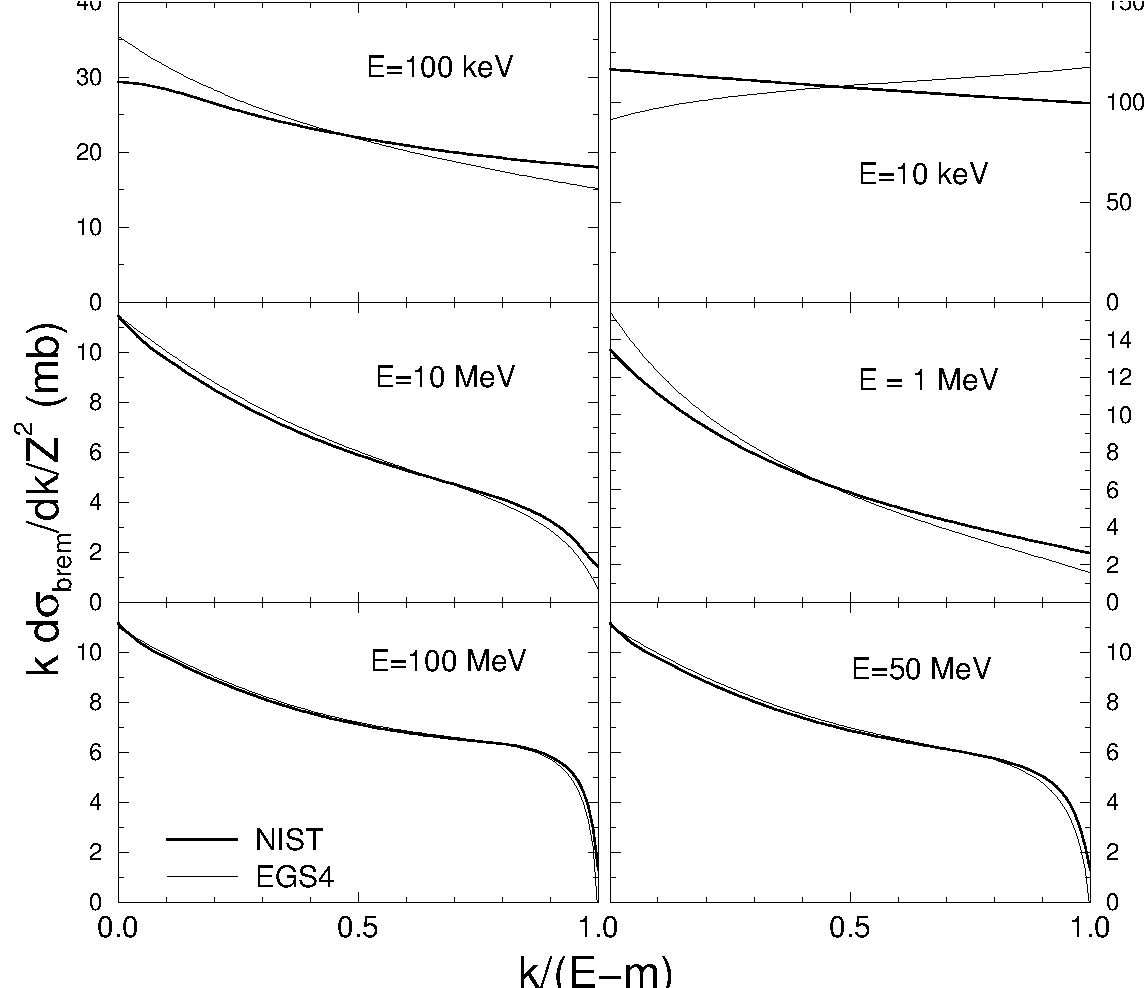
\includegraphics[height=15cm,width=15cm]{figures/brem79}
\caption[Bremsstrahlung cross sections]{\label{brems_fig1}
Differential bremsstrahlung cross sections
for gold at various incident electron energies from the NIST data base
\protect\cite{SB85,SB86a} (thick lines) compared to the
default EGSnrc (and EGS4) cross sections (thin lines). In both cases {\tt
IAPRIM = 1}, which is the default in the EGSnrc system and was an option
in the EGS4 system.}
\index{IAPRIM} \index{ibr\_nist}
\end{figure}
The behaviour for other materials is qualitatively similar.
As one can expect, the two cross sections are virtually
identical at high energies, but there are significant differences
at low energies (although the radiative stopping power is the
same due to the use of $A'$ from Eq. (\ref{brems_aprime})).

\paragraph{Simulation of discrete bremsstrahlung events, photon energy}
\hfill
\index{bremsstrahlung!simulation of}
\index{discrete interactions!bremsstrahlung}


In the course of the re-work of the EGS4 sampling routines
we have found an error in the sampling algorithm used in
EGS4. The error, which was most likely not discovered before
because it shows up only if the incident electron energy is
not much larger than the threshold energy $k_c$, is
demonstrated in Fig. \ref{brems_fig2}. This figure compares the distribution
sampled by the EGS4 routine {\tt BREMS} (points) for 100 keV
electrons in aluminum, expressed in
terms of $x$,
\begin{equation}
\label{brems_x}
x = {\ln k/k_c \over \ln T/k_c}~,
\end{equation}
to the theoretically expected result (solid line). The threshold
energy $k_c$ was 10 keV ($k_c$ is called {\tt AP} in EGS4 and EGSnrc).
%${\rm d}\sigma_{\rm brem}/{\rm d}x =
\begin{figure}[htp]
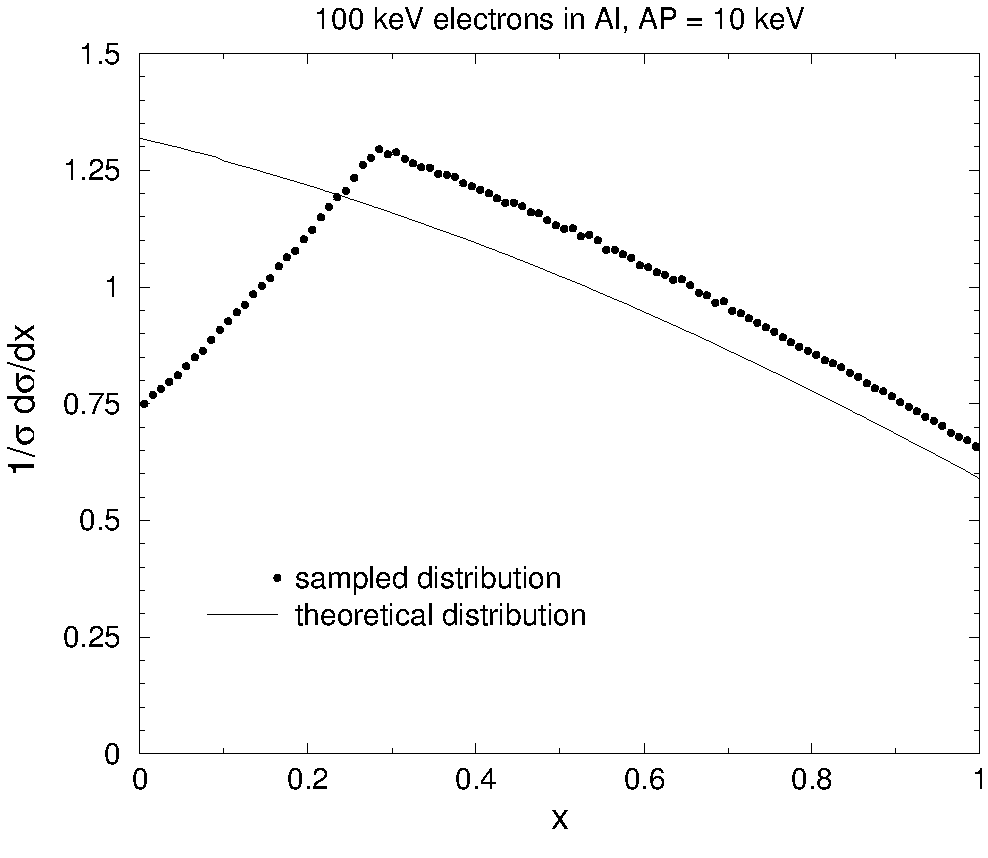
\includegraphics[height=12cm,width=12cm]{figures/Al_100keV}
\caption[{\tt BREMS} bug in EGS4]{\label{brems_fig2}
The distribution of photon energies
sampled by the EGS4 routine {\tt BREMS} (points) for 100 keV
electrons in aluminum, expressed in terms of $x$, defined in
Eq. (\protect\ref{brems_x}), compared to the theoretical
expectation.}
\end{figure}
This finding was a sufficient motivation to completely recode
the {\tt BREMS} routine.

The most efficient algorithm for sampling photon energies on
the basis of Eq. (\ref{brems_cs}) appears to be the following:
after a change of variables from $k$ to $x$, we have
\begin{eqnarray}
{{\rm d} \sigma_{\rm brem}(E,Z) \over {\rm d} x} & = & C
\left\{ \left(1 + {E^{' 2} \over E^2} \right)
\left[ \phi_1(\delta) - \frac{4}{3} \ln Z - 4 \tilde{f}_c(E,Z) \right]
\right. \nonumber \\ & - & \left.
\frac{2}{3}~\frac{E'}{E} \left[\phi_2(\delta) -
\frac{4}{3} \ln Z - 4 \tilde{f}_c(E,Z) \right]
\right\}
\end{eqnarray}
where $C$ is a constant combining factors irrelevant for
the sampling algorithm. Apart from a normalization
constant, the function in the curled brackets, to be denoted
in what follows with $R$, is the
quantity $k {\rm d}\sigma_{\tt brem}/{\rm d}k/Z^2$, shown
with the thin lines in Fig. \ref{brems_fig1}. As can be seen,
it is relatively flat and can therefore be employed as a
rejection function in conjunction with a uniform sampling
of $x$. $R$ retains its absolute maximum\footnote{The actual maximum
for a threshold energy
$k_c$ is slightly smaller and obtained for $k=k_c$, the difference between the
two is negligible except at low electron energies.}, $R_{\rm max}$, for
$k = 0$. It is given by
\begin{equation}
R_{\rm max} = 28.381 - \frac{4}{3} Z_V
\end{equation}
where $Z_V$ is defined in Eq. (\ref{pair_replace}) in section \ref{pair}
and we have made use of Eq. (\ref{pair_phi}) for the functions
$\phi_1(\delta)$ and $\phi_2(\delta)$.
The algorithm is then
\begin{enumerate}
\item
Calculate $b = \ln T/k_c$ \footnote{As the logarithm of the kinetic
energy is known prior to the call to the {\tt BREMS} routine
(because also used for other purposes), the time consuming
evaluation of the logarithm is not necessary if $\ln(k_c)$ is
stored in the computer memory for each medium.}
\item
Pick two random numbers, $r_1$ and $r_2$
\item
Set $k = k_c \exp(r_1 b)$, calculate $R/R_{\rm max}$
\item
If $r_2 > R/R_{\rm max}$, go to step 2
\item
Deliver $k$
\end{enumerate}
Figure \ref{brems_times} shows CPU times in $\mu$s necessary to sample one
photon energy on a 500 MHz PIII computer
using the new algorithm (solid line),
the EGS4 algorithm (dotted line) and using the alias sampling technique
in the case {\tt ibr\_nist} is set to 1.
\index{ibr\_nist}
\begin{figure}[htp]
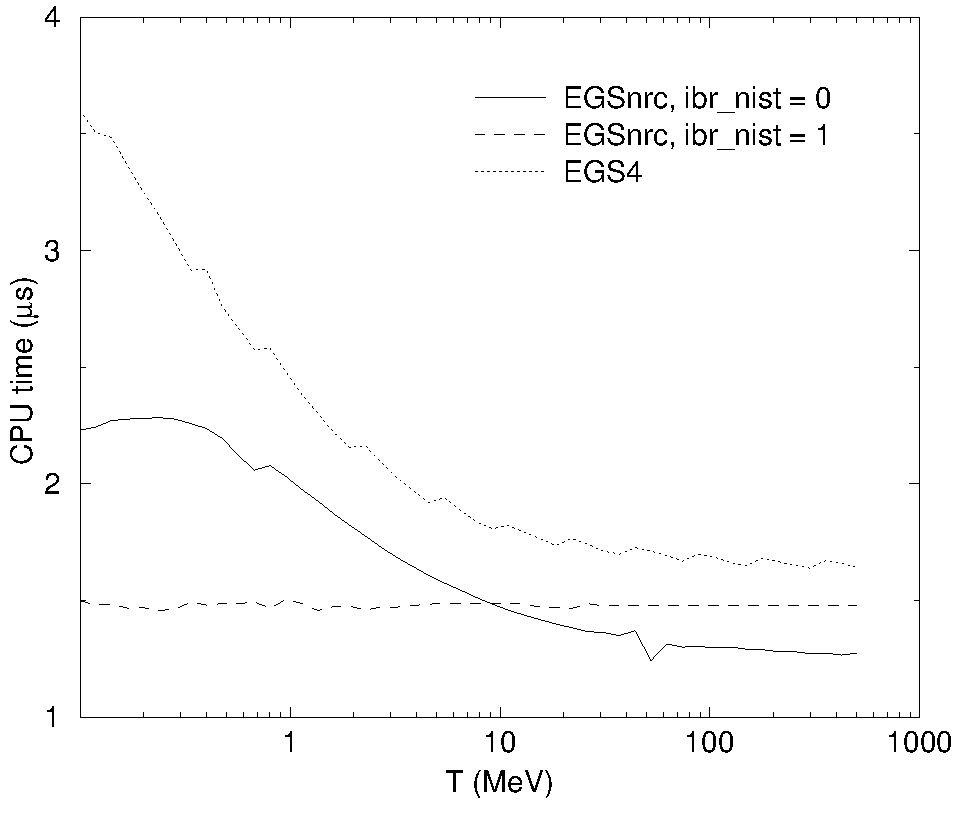
\includegraphics[height=12cm,width=12cm]{figures/brem_times}
\caption[CPU times for bremsstrahlung sampling]{\label{brems_times}
CPU times (in $\mu$s), as function of the incident electron kinetic
energy $T$, necessary to sample one photon energy using various
algorithms}
\end{figure}
The threshold energy used was $k_c = 10$~keV and the material
was aluminum. The precise
amount of CPU time spent for sampling the photon energy
is somewhat dependent on $k_c$ and $Z$, but the qualitative
behaviour remains the same for other values of $k_c$.
Apart from being more accurate, the new algorithm is also more
efficient. The CPU time for the alias sampling technique is
energy independent, as one can expect. It is faster at lower
energies but slower at high energies and so the use
of the {\tt ibr\_nist=1} option is not meaningful above 50 MeV
(where also the cross sections are identical). The small
``waves'' in the EGS4 curves are due to the technique employed
to sample the distribution $(1-\varepsilon)/\varepsilon$
(see the EGS4 manual, Ref \cite{Ne85}) which is at the same time
the reason for the error shown in Fig. \ref{brems_fig2}.
\index{SLAC-265}

\paragraph{Simulation of discrete bremsstrahlung events,
angular distribution}
\hfill
\index{bremsstrahlung!angular distribution}

In the original EGS4 implementation, the polar angle of bremsstrahlung
emission with respect to the initial electron direction was fixed
and given by $m/E$. In Ref. \cite{Bi89} an improved angle selection
scheme based on equation 2BS in the article by Koch and Motz \cite{KM59}
was implemented for use with EGS4. This implementation
was adopted in EGSnrc with slight modifications.
\index{Bielajew, Alex}

Equation 2BS, which is the bremsstrahlung cross section,
differential in the photon energy
$k$ and the photon emission angle $\theta$, is \cite{KM59}
\begin{eqnarray}
\label{brems_angle}
{\rm d}\sigma_{\rm brem}(k,\theta) & = & 4 \alpha Z^2 r_0^2 \frac{{\rm d}k}{k}
{y {\rm d} y \over (y^2 + 1)^2}
\left\{ {16 y^2 r \over (y^2 + 1)^2} - (1+r)^2 + \left[
1 + r^2 - {4 y^2 r \over (y^2 + 1)^2} \right] \ln M(y) \right\}
\nonumber \\
r & = & \frac{E'}{E}~, \quad y = \frac{E}{m} \theta~, \quad \frac{1}{M(y)} =
\Delta^2 + \left( {Z^{1/3} \over 111 (y^2 + 1)} \right)^2
\end{eqnarray}
where all definitions following Eq. (\ref{brems_cs}) apply.
Eq. (\ref{brems_angle}) is the result of an extreme relativistic,
first Born and small angle approximation, but it includes a
screening correction
based on a Thomas-Fermi potential. The effect of the screening
of the nucleus by atomic electrons is contained by the
expression in the brackets for $1/M(y)$. This can easily be
verified by comparing Eq. (\ref{brems_angle}) to equation
2BN(a) from the article by Koch and Motz which is derived
with the same approximations but using a bare nuclear potential.
In order to investigate the performance of
Eq. (\ref{brems_angle}) at low incident electron energies,
we can compare it to formula
2BN of the article by Koch and Motz which is for a bare
nucleus but does not involve the extreme relativistic
and small angle
approximations. For a ``fair'' comparison, screening corrections
must be negligible, this is the case if
\begin{equation}
\Delta^2 \gg \left( {Z^{1/3} \over 111 (y^2 + 1)} \right)^2 \quad
\mbox{or} \quad {k m \over E^2} \gg {2 Z^{2/3} \over 111^2}~,
\end{equation}
a condition which is satisfied in a wide range of photon/electron
energy combinations.
\begin{figure}[htp]
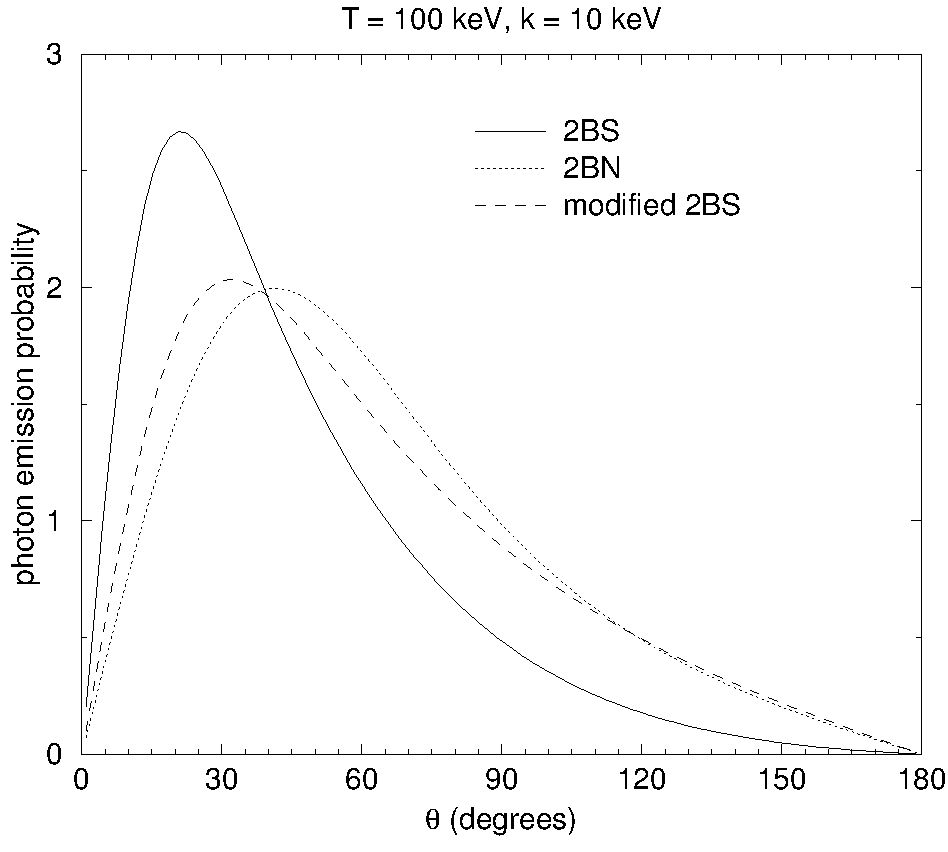
\includegraphics[height=12cm,width=12cm]{figures/bremang1}
\caption[Low energy bremsstrahlung angular distribution]{\label{brems_angle_fig1}
Angular distribution for emission of 10 keV bremsstrahlung photons
by 100 keV electrons in aluminum. Solid line represents
equation 2BS of Koch and Motz (Eq. (\ref{brems_angle}) in this
report), the dotted line equation 2BN of Koch and Motz, the
dashed line is 2BS with modifications as discussed in the text.}
\end{figure}
Figure \ref{brems_angle_fig1} shows a typical result of such
a comparison. The modification to 2BS that we have undertaken,
shown as a dashed line and obviously at a much better
agreement with formula 2BN,
is fairly simple and allows most of the considerations of
Ref.~\cite{Bi89} to be applied for the sampling procedure.
We note that the leading term of the distribution
2BN is $(1 - \beta \cos \theta)^{-2}$ where $\beta$ is the
electron velocity in units of the speed of light.
Approximated for
small angles and high energies it is equivalent to
the leading term of 2BS $(1 + y^2)^{-2}$, apart from a
normalization constant:
\index{Bielajew, Alex}
\begin{eqnarray}
(1 - \beta \cos \theta)^2 & \approx &
\left[1 - \beta\left(1 - \frac{\theta^2}{2}\right)\right]^2 =
(1 - \beta)^2 \left[ 1 + \theta^2 {\beta \over 1 - \beta} \right]^2
\nonumber \\
& = & (1 - \beta)^2 \left(1 + \beta (1 + \beta) \theta^2 \frac{E}{m} \right)^2
\approx (1 - \beta)^2 (1 + y^2)^2
\end{eqnarray}
We then use
\begin{equation}
y^2 = \beta (1 + \beta) \frac{E^2}{m^2} (1 - \cos \theta)
\end{equation}
in Eq. (\ref{brems_angle})\footnote{One could go one step
further and modify terms containing $y^2$ in the nominator
as they obviously come from expressions with $\sin^2 \theta$ but
this turns out to not improve the agreement to 2BN significantly}
and otherwise apply the results of
Ref. \cite{Bi89} so that the sampling algorithm is as follows:
\begin{enumerate}
\item
Calculate the maximum of the function in the curled brackets (to be
denoted by $f(y)$),
$f_{\rm max}$,
which is obtained for $y^2 = 0, y^2 = 1$ or $y^2 = y_{\rm max}^2 \equiv
2 \beta (1 + \beta) (E/m)^2$ for the current $E$ and $k$
\item
Pick two random numbers $r_1$ and $r_2$
\item
Sample $y^2$ from $y {\rm d}y/(1+y^2)^2$ using
\begin{equation}
y^2 = {r_1 y_{\rm max}^2 \over 1 + y_{\rm max}^2 (1 - r_1)}
\end{equation}
\item
If $r_2 > f(y)/f_{\rm max}$ go to step 2
\item
Deliver $\cos \theta$,
\begin{equation}
\cos \theta = 1 - {y^2 m^2 \over \beta (1 + \beta) E^2}
= 1 - \frac{y^2}{2 y_{\rm max}^2}
\end{equation}
\end{enumerate}
\index{IBRDST}
The efficiency of this algorithm is close to unity for low
energies and decreases logarithmically with increasing energy.
In addition, it requires several logarithm evaluations
(3 in step 1, 1 for each repetition of step 4) and is therefore
rather slow. We have therefore implemented a second bremsstrahlung
angle selection scheme which uses only the leading term of
the angular distribution and can be selected by the user
by setting the parameter {\tt IBRDST} in {\tt COMMON/BREMPR/} to zero
(the default {\tt IBRDST} value is 1,
{\em i.e.} modified 2BS from Koch and Motz).
We have found that the original
EGS4 fixed angle approach is not faster than using the
leading term of the angular distribution and have
therefore removed it.
\index{Bielajew, Alex}

\paragraph{Radiative splitting} \hfill
\label{rad_split}
\index{radiative splitting}
\index{bremsstrahlung!splitting}
\index{nbr\_split}
\index{variance reduction!brem splitting}

If the radiative splitting option is set ({\tt nbr\_split} $> 1$),
the result of a bremsstrahlung event will be {\tt nbr\_split}
photons, each having the fraction 1/{\tt nbr\_split} of
the weight of the electron, and an electron with an
energy given by its initial energy minus the energy of
the last bremsstrahlung photon produced. Note that
this violates energy conservation on an event-by-event
basis, energy is conserved only on average. The
motivation to ``inline'' the bremsstrahlung splitting technique
was that various quantities, necessary for the sampling
of photon energies, emission angles, and associated
rotations, can be calculated only once and then re-used
{\tt  nbr\_split} times.

It is worth noticing that if {\tt nbr\_split} is set
to zero, the bremsstrahlung event will be skipped.
This gives the possibility to study, for instance, the
influence of the neglect of bremsstrahlung production
on calculated quantities\footnote{A similar result
can be achieved by using {\tt IUNRST=4} when generating
the PEGS data but in this case the average energy lost to radiation
will be still subtracted and deposited locally.}, should
this be of any use to someone.

\subsubsection{Discrete inelastic collisions}
\label{discrete_inel}
\setcounter{equation}{0}
\index{inelastic collisions}
\index{binding effects}
\index{electron impact ionization}
\index{discrete interactions!inelastic collisions}

%At the present stage, binding effects are disregarded
%in the treatment of electron and positron inelastic
%scattering with atomic electrons in EGSnrc
%(and also in the default EGS4  version).
%Namito {\em et al} have implemented various
%electron impact ionization cross sections for
%use with EGS4 \cite{Na98}. We have studied their approach
%but decided to postpone the inclusion
%of binding effects until a more general treatment
%becomes available that can easily be applied
%to ``catastrophic'' {\em and} sub-threshold inelastic
%collisions.

When the binding of atomic electrons is ignored (default EGSnrc behavior),
electron-electron scattering can be described by the
M{\o}ller cross section \cite{Mo32a} and
positron-electron scattering by the Bhabha cross section
\cite{Bh35}. When binding is taken into account, interactions of
electrons and positrons with atoms can result in the creation of inner
shell vacancies, this process is usually referred to as electron impact
ionization (EII).

\paragraph{M{\o}ller scattering} \hfill
\index{M{\o}ller cross section}
\index{M{\o}ller scattering}
\index{discrete interactions!M{\o}ller scattering}
\index{cross section!M{\o}ller}

The M{\o}ller cross section, which is the cross section
for electron-electron scattering differential in the kinetic energy
$T'$ of the scattered electron which is initially at rest, is
\cite{ICRU37}
\begin{equation}
\label{moller_cs}
{{\rm d} \sigma_{\rm inel}^- \over  {\rm d}T'} =
{2 \pi r_0^2 m \over \beta^2}~\frac{1}{T^{\prime 2}} \left[
1 + {T^{' 2} \over (T - T')^2} + {\tau^2 \over (\tau+1)^2}~
\left(\frac{T'}{T}\right)^2
- {2 \tau + 1 \over (\tau + 1)^2}~{T' \over T - T'} \right]
\end{equation}
where $\beta$ is the incident electron velocity in units of the
speed of light, $T$ the incident kinetic energy and $\tau = T/m$.
Because the two electrons are indistinguishable, Eq. \eqref{moller_cs}
is symmetric with respect to exchange of the energies of the two scattered
particles. Per definition, the electron with the higher energy
after the collision is considered to be the primary, so that
the total cross section for M{\o}ller interactions is obtained
via integration of Eq. \eqref{moller_cs} from $T_c$ to $T/2$:
\begin{equation}
\label{moller_cs1}
\sigma_{\rm inel}^- = \int\limits_{T_c}^{T/2}
{{\rm d} \sigma_{\rm inel}^- \over  {\rm d}T'} {\rm d}T'
\end{equation}
\index{TE}
\index{AE}
In EGS4 and EGSnrc $T_c$ is called {\tt TE} and the corresponding
total energy {\tt AE}. The threshold kinetic energy above which M{\o}ller
events can occur is obviously $2 T_c$. The integration of
Eq. \eqref{moller_cs1} is trivial, and is evaluated by the
PEGS function {\tt AMOLTM}.
\index{AMOLTM}
\index{PEGS4!AMOLTM}

\index{M{\o}ller scattering!sampling of}
To sample the energy of the scattered electron on the basis of
Eq. \eqref{moller_cs}, one makes a change of variables to
$\varepsilon = T'/T$, which can take values between
$\varepsilon_0  = T_c/T$ and $1/2$, and after re-arranging
obtains \cite{Ne85}
\begin{equation}
\label{moller_cs2}
{{\rm d} \sigma_{\rm inel}^- \over  {\rm d} \varepsilon} =
C \left( {\varepsilon_0 \over 1 - 2 \varepsilon_0}~\frac{1}{\varepsilon^2}
\right) g(\varepsilon)
\end{equation}
where $C$ is a constant irrelevant for the sampling algorithm,
the expression in the brackets is a normalized PDF for $\varepsilon$
and $g(\varepsilon)$ will be used as a rejection function.
At this point it is worth noticing that there is an error in the EGS4 manual
for the rejection function $g(\varepsilon)$ and the resulting error
in the {\tt MOLLER} sampling routine was not
corrected in EGS4 until 1996 \cite{Bi96b}. The proper rejection function
reads
\index{SLAC-265}
\index{Bielajew, Alex}
\begin{equation}
\begin{split}
g(\varepsilon) &= {1 + g_2 \varepsilon^2 + r (r - g_3) \over
g_{\rm max} } \\ g_{\rm max} &= 1 + \frac{5}{4} g_2~, \quad
g_2 = {\tau^2 \over (\tau + 1)^2}~, \quad g_3 = {2 \tau + 1 \over (\tau+1)^2}~,
\quad r = {\varepsilon \over 1 - \varepsilon } ~.
\end{split}
\end{equation}
The algorithm used to sample $\varepsilon$ is then as follows:
\begin{enumerate}
\item
Calculate quantities dependent only on $T$, namely
\begin{displaymath}
\tau,~g_2,~g_3,~g_{\rm max}
\end{displaymath}
\item Pick two random numbers, $r_1$ and $r_2$
\item Sample $\varepsilon$ from the expression in the brackets in
Eq. \eqref{moller_cs2} using
\begin{equation}
\varepsilon = {T_c \over T - (T - 2 T_c) r_1}
\end{equation}
\item Calculate $g(\varepsilon)$, if $r_2 > g(\varepsilon)$  go to step 2
\item Deliver $\varepsilon$
\end{enumerate}
The efficiency of this algorithm is close to unity for
low incident energies $T$ but goes to $4/9$ at high energies.
A better approach would be the following: We can rewrite
Eq. \eqref{moller_cs1} as
\begin{equation}
\begin{split}
{{\rm d} \sigma_{\rm inel}^- \over  {\rm d}T'} & =
{2 \pi r_0^2 m \over \beta^2}~ \left[ F(T') + F(T-T') \right] \\
F(T') &= \frac{1}{T^{\prime 2}} + {1 \over 2 (T+m)^2} -
{2 \tau + 1 \over (\tau+1)^2}~\frac{1}{T T'} ~.
\end{split}
\end{equation}
If we now extend the range for $T'$ to $T-T_c$, we can drop
$F(T-T')$, and sample $T'$ from $F(T')$ only. At the end
$T'$ will be set to Min$(T',T-T')$. There are several possibilities
to sample $T'$ from $F(T')$. For instance, one can use
$1/T^{\prime 2}$ as a PDF and
\begin{equation}
g'(T') = \frac{1}{g'_{\rm max}} \left(1 + {T^{\prime 2} \over 2 (T+m)^2}
- {2 \tau + 1 \over (\tau + 1)^2}~ \frac{T'}{T} \right)
\end{equation}
as a rejection function. Here,
\begin{equation}
g_{\rm max} = \left\{
\begin{array}{r@{~~, \quad}l}
1 & \text{if}~~ \tau \le 2 + \sqrt{6} \\
{3 \tau^2 \over 2 (\tau+1)^2 } & \text{else}
\end{array} \right.
\end{equation}
The efficiency of such an algorithm is $2/3$ at high energies and
therefore 1.5 times better than the one used in EGS4 and EGSnrc.
Anticipating changes in the treatment of discrete inelastic
scattering, in order to take into account electron binding
effects, in the near future we have not implemented
this more efficient algorithm.

The polar scattering angles $\theta$ and $\theta'$
in M{\o}ller events are uniquely
determined by the kinematics. They are given by
\begin{equation}
\label{moller_angles}
\begin{split}
\cos \theta & = \sqrt{\frac{T-T'}{T}~\frac{T+2 m}{T-T' + 2 m}}~, \quad
\text{for the higher energy electron,} \\
\cos \theta' & = \sqrt{\frac{T'}{T}~\frac{T+2 m}{T' + 2 m}}~, \quad
\quad \quad \quad \quad  \text{for the lower energy electron.}
\end{split}
\end{equation}
The azimuthal angles are opposite and sample uniformly between
zero and $2 \pi$.

\paragraph{Bhabha scattering} \hfill
\index{Bhabha cross section}
\index{Bhabha scattering}
\index{discrete interactions!Bhabha scattering}
\index{cross section!Bhabha}

The Bhabha cross section, which is the cross section
for positron-electron scattering differential in the kinetic energy
$T'$ of the scattered electron which is initially at rest, is
given by \cite{Ne85}
\begin{equation}
\label{bhabha_cs}
{{\rm d} \sigma_{\rm inel}^+ \over  {\rm d}T'} =
{2 \pi r_0^2 m \over T^2} \left[ \frac{1}{\varepsilon}\left(
{1 \over \varepsilon \beta^2} - B_1 \right) + B_2 + \varepsilon
(\varepsilon B_4 - B_3 ) \right]
\end{equation}
where $T$ is the incident positron kinetic energy and
the following definitions apply:
\begin{equation}
\label{vhabha_cs1}
\begin{split}
\varepsilon & = \frac{T'}{T}, \quad \tau = \frac{T}{m},
\quad y = {1 \over \tau + 2}, \quad \beta^2 = {\tau (\tau + 2) \over
(\tau + 1)^2} \\
B_1 &= 2 - y^2, \quad B_2 = (1 - 2 y)(3 + y^2), \quad B_3 = B_4 +
(1 - 2 y)^2, \quad B_4 = (1 - 2 y)^3
\end{split}
\end{equation}
The range of possible $T'$ values is $T_c \cdots T$
({\em i.e.} the positron may have energy less then $T_c$
after Bhabha scattering).
The total discrete Bhabha cross section is then obtained
by integrating Eq. \eqref{bhabha_cs} in the allowed range,
{\em i.e.}
\begin{equation}
\sigma_{\rm inel}^+ = \int\limits_{T_c}^T {\rm d}T'
{{\rm d} \sigma_{\rm inel}^+ \over  {\rm d}T'}~.
\end{equation}
The integration is trivial but the result rather lengthy and therefore not
given here. The total discrete Bhabha cross section is evaluated
by the PEGS function {\tt BHABTM}.
\index{PEGS4!BHABTM}

\index{Bhabha scattering!sampling of}
The method employed to sample scattered electron energies on the basis
of Eq. \eqref{bhabha_cs} is similar to the M{\o}ller method.
The electron energy fraction $\varepsilon$ is sampled from
$1/\varepsilon^2$, the rejection function $g(\varepsilon)$ is
\begin{equation}
g(\varepsilon) = 1 - \beta^2 \varepsilon (B_1 - \varepsilon (B_2
- \varepsilon (B_3 - \varepsilon B_4)))~.
\end{equation}
As in the case of M{\o}ller scattering, there was an error for
the Bhabha scattering rejection function which was not corrected
until 1996 \cite{Bi96b}. Bhabha polar scattering angles are
given by Eq. \eqref{moller_angles}.
\index{Bielajew, Alex}

\subsubsection{Electron Impact Ionization}
\label{discrete_eii}
\setcounter{equation}{0}
\index{binding effects}
\index{electron impact ionization}
\index{discrete interactions!electron impact ionization}

Since 2003 the EGSnrc system has the ability to explicitely
simulate the creation of inner shell vacancies by electron or positron
impact for all K- and L-shells with binding energies above 1 keV.
This option can be turned on by setting the parameter {\tt eii\_flag} found
in {\tt COMIN/EII-DATA} to one. The differential cross sections used are
based on a semi-empirical theory described in Ref. \cite{Ka02b}. By default,
total EII cross sections are obtained by a numerical integration from these
differential cross sections. However, the user has the option to use
total EII cross sections from Gryzi\'{n}ski \cite{Gr65a}, Casnati \cite{Ca82}
Kolbenstvedt \cite{Ko67}, or Bote and Salvat \cite{BS08}.
This is accomplished by changing the parameter
{\tt eii\_xfile} found in {\tt COMIN/MEDIA} to {\tt gryzinski, casnati, kolbenstvedt} or {\tt penelope}. Users can also use their own
set of EII cross sections by setting
{\tt eii\_xfile} to an arbitrary charater string.
See section \ref{step_2} on page \pageref{eii_xfile_description}
for more detials.

When EII is turned on and there are K- or L-shells with
binding energies above {\tt AE} or {\tt AP} in the medium where a discrete
inelastic collision takes place, the probability for the collision being
with the K- or L-shell is computed. If a random number is less than this probability,
the interaction is simulated according to the EII differential cross sections of
Ref. \cite{Ka02b} and an inner shell vacancy is created that is subsequently relaxed
\index{relaxations}
using the subroutine {\tt RELAX} (see section \ref{relax}). Otherwise the
interaction is simulated according to the M{\o}ller or Bhabha cross sections.

\subsubsection{Two Photon Positron-Electron Annihilation}
\setcounter{equation}{0}
\label{annihilation}
\index{annihilation}
\index{positron annihilation}
\index{discrete interactions!annihilation}
\index{cross section!annihilation}

We have adopted the treatment
of the two photon positron annihilation process  from
EGS4 without modifications. For completeness
we give below the differential and total annihilation
cross sections as used in EGS4 and EGSnrc.

The cross
section, differential in the energy $k$ of the one
of the annihilation photons, for an incident positron with
a total energy of $E$ is \cite{Ne85}
\begin{equation}
\label{annih_cs}
{{\rm d} \sigma_{\rm annih} \over {\rm d} k} = {\pi r_0^2 \over \tau
(\tau+2)} \left[ S_1(\kappa) + S_1(\tau + 2 - \kappa) \right]
\end{equation}
where $\tau$ and $\kappa$ are the positron kinetic energy and photon
energy in units of $m$ and
\begin{equation}
S_1(x) = \frac{1}{x} \left( \tau + 2 + 2 {\tau + 1 \over \tau + 2} -
\frac{1}{x} \right) - 1~.
\end{equation}
Equation (\ref{annih_cs}) is obviously symmetric
under exchange of the annihilation photons,
the second photon has the energy $E + m - k$.

The polar emission angles of the annihilation photons are uniquely
determined by the kinematics and given by \cite{Ne85}
\begin{equation}
\label{annih_k_theta}
k = { m \over 1 - a \cos \theta}~,
\quad a = \sqrt{{\tau \over \tau + 2}}
\end{equation}
so that the minimum and maximum possible photon energies are
\begin{equation}
\label{annih_kminmax}
k_{\rm min} = {m \over 1 + a} ~, \quad
k_{\rm max} = {m \over 1 - a}~.
\end{equation}
The total annihilation cross section
is obtained by integrating Eq. (\ref{annih_cs})
over the allowed $k$-range and can be written as
\begin{equation}
\sigma_{\rm annih} = {\pi r_0^2 \over \tau + 2} \left[
{\tau^2 + 6 \tau + 6 \over \tau (\tau + 2)} \ln\left(\tau + 1
+ \sqrt{\tau (\tau + 2)} \right) - {\tau + 4 \over \sqrt{\tau (\tau + 2)}}
\right]
\end{equation}
At high energies ($\tau \gg 1$) $\sigma_{\rm annih}$
decreases as $(\ln \tau)/\tau$, for $\tau \to 0$ the cross section
tends to infinity ({\em i.e.} positrons always annihilate at rest
if they have not annihilated before).

The annihilation process is a ``catastrophic'' event and
treated discretely.

\index{annihilation!sampling of}
To sample the energy of one of the photons from
Eq. (\ref{annih_cs}), one makes a change in variables
to $\varepsilon = \kappa/(\tau+2)$, drops the second
$S_1$ because of the symmetry, and after re-arranging obtains
\begin{eqnarray}
{{\rm d} \sigma_{\rm annih} \over {\rm d}\varepsilon} & = &
C f(\varepsilon) g(\varepsilon) \\
f(\varepsilon) & = & {1 \over \ln[(1-\varepsilon_0)/\varepsilon_0]}~
\frac{1}{\varepsilon}~, \quad
%g(\varepsilon) = 1 - \varepsilon + {2 (\tau + 1) \varepsilon - 1 \over
%(\tau + 2)^2 }
g(\varepsilon) = 1 - {[\varepsilon (\tau+2) - 1) ]^2 \over \varepsilon
(\tau^2 + 4 \tau + 2) }
\end{eqnarray}
where $C$ is a constant that contains factors irrelevant for
the sampling procedure and $\varepsilon_0$ the minimum
possible value for $\varepsilon$,
\begin{equation}
\varepsilon_0 = {1 \over (\tau+2) (1 + a)}~.
\end{equation}
The function $f(\varepsilon)$ is a normalized PDF, $g(\varepsilon)$
is always positive and
has a maximum
of $1$ for $\epsilon = 1/(\tau+2)$ and
thus is a valid rejection function\footnote{Note that our $g(\varepsilon)$ is
the $g(\varepsilon)$ defined in Eq (2.12.26) of the EGS4 manual
divided by its maximum.}. The sampling algorithm is then as follows:
\begin{enumerate}
\item
Compute quantities dependent on $E$, namely
\begin{displaymath}
\tau,~A = \tau+2,~a,~\varepsilon_0,~
b = \ln{1 - \varepsilon_0 \over \varepsilon_0}
\end{displaymath}
\item
Pick two random numbers, $r_1$ and $r_2$
\item
Set
\begin{equation}
\varepsilon = \varepsilon_0 \exp\left(r_1 b\right)
\end{equation}
and calculate $g(\varepsilon)$
\item
If $r_2 > g(\varepsilon)$, the go to step 2
\item
Deliver $\varepsilon$
\end{enumerate}

\index{annihilation!single photon}
\index{annihilation!three photon}
At this point
one should perhaps mention that a single photon or three or more
photon annihilation processes in the nuclear field are also
possible. Messel and Crawford \cite{MC70} point out that
the ratio of one to two photon annihilation cross sections is small
until higher energies are reached, at which point the absolute
value of the cross section is small. Thus, the single
photon annihilation process is ignored. Positron annihilation to
three or more photons is even less likely than one photon
annihilation and therefore also ignored.

\index{annihilation!at rest}
If positrons do not annihilate in flight, they
annihilate at rest producing two photons. As one can easily
verify from Eq. \eqref{annih_k_theta} and \eqref{annih_kminmax},
the photon energies go to $m$ as $\tau$ goes to zero.
In addition, the cross section differential in the
photon emission angle becomes uniform in the limit $\tau \to 0$.

\index{radiative splitting}
\index{variance reduction!radiative splitting}
\index{nbr\_split}
If radiative splitting is set ({\tt nbr\_split} $> 1$),
the annihilation process will produce 2 {\tt nbr\_split} photons,
each carrying the fraction 1/{\tt nbr\_split} from the positron weight.
Simultaneous production of {\tt nbr\_split} annihilation
events allows the quantity $b$ (see step 1) as well as
parameter related to angular rotations to be re-used
{\tt nbr\_split} times.

\subsubsection{Collision stopping power}
\label{stopping_power}
\setcounter{equation}{0}
\index{stopping powers}
\index{restricted stopping powers}
\index{collision stopping powers}

\index{Seltzer, Stephen}
\index{Berger, Martin}
EGSnrc ``inherits'' the treatment of restricted collision
stopping powers from EGS4, {\em i.e.} uses the formulas
recommended by Seltzer and Berger \cite{BS64} which are based
on the Bethe-Bloch theory \cite{Be30,Be32,Bl33}. The standard
treatment (see also ICRU report 37 \cite{ICRU37} which was
used as the source of the formulas below)
assumes that there is a certain value for energy
transfer to atomic electrons, $T_{\rm med}$, that is (i)
large compared to the binding energies (ii) corresponds to
an impact parameter that is large compared to the atomic
dimensions. Collision processes that are associated with
energy loss $T'$ less than $T_{\rm med}$ are treated according to
the theory of Bethe, the main result of which is that
\begin{equation}
L_{\rm coll}^\pm(T,T' < T_{\rm med}) = {2 \pi r_0^2 m n \over \beta^2}
\left[ \ln \left(2 m \beta^2 T_{\rm med} \over (1 - \beta^2) I^2 \right)
- \beta^2 - \delta \right]
\end{equation}
where $\beta$ is again the electron velocity in units of
the speed of light, $I$ is the mean ionization energy and
$\delta$ the density effect correction that takes into
\index{density effect}
account the polarization of the medium due to the electron field.
As $T_{\rm med}$ is defined being large compared to the binding energies of
the atom, collision processes with energy transfer larger
than $T_{\rm med}$ can be treated using the M{\o}ller \cite{Mo32a} (electrons)
or Bhabha \cite{Bh35} (positron) cross section (see also section
\ref{discrete_inel}), {\em i.e.}
\index{$T_{\rm med}$}
\index{M{\o}ller cross section} \index{Bhabha cross section}
\begin{equation}
L_{\rm coll}^\pm(T,T' > T_{\rm med}) = \int\limits_{T_{\rm med}}^{T_c}
{\rm d}T' T' {{\rm d} \sigma_{\rm inel}^\pm \over {\rm d}T'}
\end{equation}
Using some additional approximations, $T_{\rm med}$ drops out
in the sum of $L_{\rm coll}^\pm(E,T' < T_{\rm med})$ and
$L_{\rm coll}^\pm(E,T' > T_{\rm med})$ and one obtains
\begin{equation}
L_{\rm coll}^\pm(T,T_c) = {2 \pi r_0^2 m n \over \beta^2}
\left[ \ln {T^2 \over I^2} + \ln(1 + \tau/2) + G^\pm(\tau) - \delta \right]
\end{equation}
where $\tau = T/m$ and the functions $G^\pm$ are different for
electrons and positrons due to differences in the M{\o}ller and
Bhabha cross sections and are given by
\index{Bhabha scattering}
\begin{equation}
\begin{split}
G^-(\tau) & = -1 - \beta^2  + \ln\left[4 \eta (1 - \eta) \right] +
{1 \over 1 - \eta} + (1 - \beta^2) \left[ {\tau^2 \eta^2 \over 2} +
(2 \tau + 1) \ln(1 - \eta) \right] \\
G^+(\tau) & = \ln(4 \eta) - \beta^2 \left[ 1 + (2 - y^2) \eta -
(3 + y^2) {y \tau \over 2} \eta^2 + (1 + y \tau) {y^2 \tau^2 \over 3} \eta^3
- {y^3 \tau^3 \over 4} \eta^4
\right]
\end{split}
\end{equation}
where $\eta = T_c/T$ and $y$ is defined in Eq. \eqref{bhabha_cs}.

\index{Class II scheme!validity of}
From the above discussion and from the general discussion
of a Class II condensed history implementation in section
\ref{electron_general} it is clear that the formalism
used to treat inelastic collisions with atomic electrons
is only applicable if
\begin{equation}
\label{Tc_condition}
T_c \gg ~~\text{binding energies of the medium of interest}.
\end{equation}
This imposes a rather severe limitation on the use
of Class II condensed history codes in high-$Z$ materials
(the $K$-shell binding energy for lead is, for instance, 88 keV).
We are therefore currently investigating a more realistic approach for
situations when the condition \eqref{Tc_condition} is not
satisfied, but its implementation into EGSnrc is left for the
next release of the system. One should probably also mention
that the many successful studies carried out with the
EGS4 system indicate that the implications of violating
the requirement \eqref{Tc_condition} are perhaps less
severe than one might expect from purely theoretical arguments.

\index{mean ionization energy}
\index{density effect}
\index{stopping powers}
The only non-trivial parameters of the restricted stopping
power formula are the mean ionization energy $I$ and the
density effect correction $\delta$. The default mean ionization
energies for elements used in PEGS4, along with atomic numbers,
weights, chemical symbols, and mass densities are summarized
in Table \ref{I_values}. Mean ionization energies for
compounds are derived from
\begin{equation}
\ln I = \sum p_i Z_i \ln I(Z_i)
\end{equation}
where $p_i$ is the stoichiometric index of the $i$'th element
which has atomic number $Z_i$ and a mean ionization energy $I(Z_i)$,
unless the material belongs to a set of pre-defined materials
to be found in Table 2.13.2 of the EGS4 manual \cite{Ne85} or listed in the
{\tt BLOCK DATA} section of {\tt pegs4.mortran}.
\index{pegs4.mortran}
\index{SLAC-265}

\index{Seltzer, Stephen}
\index{Berger, Martin}
\index{ISSB}
The density effects correction
has been treated extensively in the literature.
The default PEGS4 approach is based on the formulation of Sternheimer and
Peierls\cite{SP71} which basically parameterizes the density effect in
terms of 6 parameters ({\tt AFACT, SK, X0, X1, CBAR}, and {\tt IEV}).  This same parameterized approach was used for
the calculations by Berger and Seltzer \cite{BS83} and by
Sternheimer, Berger and  Seltzer \cite{St82} who fitted the parameters to
the density effect as calculated for the ICRU for increasingly larger
numbers of materials.  The power of PEGS4 is that it will generate a
density effect for any arbitrary material, if need be with no recourse to the fitted
parameters. In this case it will use the  Sternheimer and
Peierls\cite{SP71} general formula.  There is also an option in PEGS4 which allows the 6
parameters to be read in directly (using the {\tt ISSB=1} option in PEGS4,
see section~\ref{issb} page~\pageref{issb}). However, these
parameterizations are only fits to the actual density effect data. An
option was added to PEGS4 in 1989 which allowed the density effect data
to be used directly\cite{Du89} and the EGSnrc distribution includes a huge
data base of all the density effect values calculated by Seltzer and Berger
for ICRU Report 37\cite{ICRU37}.
To turn this option on the user must
set the flag {\tt EPSTFL} to 1 in the PEGS4 input file. See
section~\ref{icru37_csp} (page~\pageref{icru37_csp}) for more details.
In this case the density effect correction is calculated
by interpolation from pre-computed values stored in
a separate file.
Selecting this option has the additional effect that the mean
ionization energy of the material is taken directly from
the density effect correction file. It should be noted that in general the
differences in collision stopping powers between using the default Sternheimer
and Peierls density effect, or the fitted parameters or the direct ICRU 37
values, are small, of the order of a few percent at most.  These
differences are only
likely of importance for very detailed work.
\index{density effect}
\index{PEGS4!EPSTFL}
\index{EPSTFL}

\begin{longtable}{|rcrrr|}
\caption{\label{I_values}Default atomic numbers, symbols, atomic weights,
mass densities, and I values for elements in PEGS4.} \\
\hline \hline
 Z & Symbol & Atomic & Density & I(eV) \\
   &        & weight & (g/cm$^3$) &  \\
\hline
\endfirsthead
\hline
\multicolumn{5}{r}%
  {\small\slshape continued from previous page} \\
\hline \hline
 Z & Symbol & Atomic & Density & I(eV) \\
   &        & weight & (g/cm$^3$) & \\
\hline
\endhead
\hline
\multicolumn{5}{r}%
  {\small\slshape continued on next page} \\ \hline
\endfoot
\hline \hline
\endlastfoot
 1 & H      &  1.00797 &  0.0808    & 19.2 \\
 2 & HE     &  4.00260 &  0.1900    & 41.8 \\
 3 & LI     &  6.93900 &  0.5340    & 40.0 \\
 4 & BE     &  9.01220 &  1.8500    & 63.7 \\
 5 & B      & 10.81100 &  2.5000    & 76.0 \\
 6 & C      & 12.01115 &  2.2600    & 78.0 \\
 7 & N      & 14.00670 &  1.1400    & 82.0 \\
 8 & O      & 15.99940 &  1.5680    & 95.0 \\
 9 & F      & 18.99840 &  1.5000    &115.0 \\
10 & NE     & 20.18300 &  1.0000    &137.0 \\
11 & NA     & 22.98980 &  0.9712    &149.0 \\
12 & MG     & 24.31200 &  1.7400    &156.0 \\
13 & AL     & 26.98150 &  2.7020    &166.0 \\
14 & SI     & 28.08800 &  2.4000    &173.0 \\
15 & P      & 30.97380 &  1.8200    &173.0 \\
16 & S      & 32.06400 &  2.0700    &180.0 \\
17 & CL     & 35.45300 &  2.2000    &174.0 \\
18 & AR     & 39.94800 &  1.6500    &188.0 \\
19 & K      & 39.10200 &  0.8600    &190.0 \\
20 & CA     & 40.08000 &  1.5500    &191.0 \\
21 & SC     & 44.95600 &  3.0200    &216.0 \\
22 & TI     & 47.90000 &  4.5400    &233.0 \\
23 & V      & 50.94200 &  5.8700    &245.0 \\
24 & CR     & 51.99800 &  7.1400    &257.0 \\
25 & MN     & 54.93800 &  7.3000    &272.0 \\
26 & FE     & 55.84700 &  7.8600    &286.0 \\
27 & CO     & 58.93320 &  8.7100    &297.0 \\
28 & NI     & 58.71000 &  8.9000    &311.0 \\
29 & CU     & 63.54000 &  8.9333    &322.0 \\
30 & ZN     & 65.37000 &  7.1400    &330.0 \\
31 & GA     & 69.72000 &  5.9100    &334.0 \\
32 & GE     & 72.59000 &  5.3600    &350.0 \\
33 & AS     & 74.92160 &  5.7300    &347.0 \\
34 & SE     & 78.96000 &  4.8000    &348.0 \\
35 & BR     & 79.80800 &  4.2000    &357.0 \\
36 & KR     & 83.80000 &  3.4000    &352.0 \\
37 & RB     & 85.47000 &  1.5300    &363.0 \\
38 & SR     & 87.62000 &  2.6000    &366.0 \\
39 & Y      & 88.90500 &  4.4700    &379.0 \\
40 & ZR     & 91.22000 &  6.4000    &393.0 \\
41 & NB     & 92.90600 &  8.5700    &417.0 \\
42 & MO     & 95.94000 &  9.0100    &424.0 \\
43 & TC     & 99.00000 & 11.5000    &428.0 \\
44 & RU     &101.07000 & 12.2000    &441.0 \\
45 & RH     &102.90500 & 12.5000    &449.0 \\
46 & PD     &106.40000 & 12.0000    &470.0 \\
47 & AG     &107.87000 & 10.5000    &470.0 \\
48 & CD     &112.40000 &  8.6500    &469.0 \\
49 & IN     &114.82000 &  7.3000    &488.0 \\
50 & SN     &118.69000 &  7.3100    &488.0 \\
51 & SB     &121.75000 &  6.6840    &487.0 \\
52 & TE     &127.60000 &  6.2400    &485.0 \\
53 & I      &126.90440 &  4.9300    &491.0 \\
54 & XE     &131.30000 &  2.7000    &482.0 \\
55 & CS     &132.90500 &  1.8730    &488.0 \\
56 & BA     &137.34000 &  3.5000    &491.0 \\
57 & LA     &138.91000 &  6.1500    &501.0 \\
58 & CE     &140.12000 &  6.9000    &523.0 \\
59 & PR     &140.90700 &  6.7690    &535.0 \\
60 & ND     &144.24001 &  7.0070    &546.0 \\
61 & PM     &147.00000 &  1.0000    &560.0 \\
62 & SM     &150.35001 &  7.5400    &574.0 \\
63 & EU     &151.98000 &  5.1700    &580.0 \\
64 & GD     &157.25000 &  7.8700    &591.0 \\
65 & TB     &158.92400 &  8.2500    &614.0 \\
66 & DY     &162.50000 &  8.5600    &628.0 \\
67 & HO     &164.92999 &  8.8000    &650.0 \\
68 & ER     &167.25999 &  9.0600    &658.0 \\
69 & TM     &168.93401 &  9.3200    &674.0 \\
70 & YB     &173.03999 &  6.9600    &684.0 \\
71 & LU     &174.97000 &  9.8500    &694.0 \\
72 & HF     &178.49001 & 11.4000    &705.0 \\
73 & TA     &180.94800 & 16.6000    &718.0 \\
74 & W      &183.85001 & 19.3000    &727.0 \\
75 & RE     &186.20000 & 20.5300    &736.0 \\
76 & OS     &190.20000 & 22.4800    &746.0 \\
77 & IR     &192.20000 & 22.4200    &757.0 \\
78 & PT     &195.08000 & 21.4500    &790.0 \\
79 & AU     &196.98700 & 19.3000    &790.0 \\
80 & HG     &200.59000 & 14.1900    &800.0 \\
81 & TL     &204.37000 & 11.8500    &810.0 \\
82 & PB     &207.19000 & 11.3400    &823.0 \\
83 & BI     &208.98000 &  9.7800    &823.0 \\
84 & PO     &210.00000 &  9.3000    &830.0 \\
85 & AT     &210.00000 &  1.0000    &825.0 \\
86 & RN     &222.00000 &  4.0000    &794.0 \\
87 & FR     &223.00000 &  1.0000    &827.0 \\
88 & RA     &226.00000 &  5.0000    &826.0 \\
89 & AC     &227.00000 &  1.0000    &841.0 \\
90 & TH     &232.03600 & 11.0000    &847.0 \\
91 & PA     &231.00000 & 15.3700    &878.0 \\
92 & U      &238.03000 & 18.9000    &890.0 \\
93 & NP     &237.00000 & 20.5000    &902.0 \\
94 & PU     &242.00000 & 19.7370    &921.0 \\
95 & AM     &243.00000 & 11.7000    &934.0 \\
96 & CM     &247.00000 &  7.0000    &939.0 \\
97 & BK     &247.00000 &  1.0000    &952.0 \\
98 & CF     &248.00000 &  1.0000    &966.0 \\
99 & ES     &254.00000 &  1.0000    &980.0 \\
100& FM     &253.00000 &  1.0000    &994.0 \\
%\hline \hline
%\end{tabular}
%\end{center}
%\end{supertabular}
%\end{table}
\end{longtable}

\subsubsection{Elastic scattering cross sections}
\label{elastic}
\setcounter{equation}{0}
\index{elastic scattering}
\index{spin effects}
\index{cross section!elastic}

\index{SPIN\_EFFECTS}
The treatment of electron and positron elastic
scattering in EGSnrc is determined by the logical parameter
{\tt SPIN\_EFFECTS} which is in {\tt common/ET\_Control/}.
If set to {\tt .true.} (this is the default),
elastic scattering cross sections
that take into account spin effects are employed, they
are discussed in section \ref{spin_elastic}. If {\tt .false.},
elastic scattering is based on the screened Rutherford cross section.
This is consistent with EGS4, although multiple elastic
\index{multiple elastic scattering}
\index{\Mol~theory}
scattering (see section \ref{sec_MS})
is based on an exact theory rather than the
small-angle theory of \Mol \cite{Mo48} which is used in EGS4.
\index{screened Rutherford cross section}

\paragraph{Screened Rutherford elastic scattering} \hfill
\index{screened Rutherford cross section}

The screened Rutherford cross section, which is the cross
section differential in the cosine $\mu$ of the polar
scattering angle of electrons or positrons incident
on atoms of atomic number $Z$, is
\begin{equation}
\label{SR_1}
{{\rm d} \sigma_{\rm SR} \over {\rm d}\mu} = {2 \pi r_0^2 Z^2 \over
\beta^2 \tau (\tau + 2) }~{1 \over (1 - \mu + 2 \eta)^2}
\end{equation}
where $\beta$ is the particle velocity in units of the speed of
light, $\tau$ the kinetic energy $T$ in units of $m$
\index{screening parameter}
and $\eta$ the screening parameter. The total elastic scattering
cross section is obtained from Eq. \eqref{SR_1} by integrating
over $\mu$ from -1 to 1 and is given by
\begin{equation}
\label{SR_2}
\sigma_{\rm SR} = {\pi r_0^2 Z^2 \over \beta^2 \tau (\tau+2) \eta (1 + \eta)}
\end{equation}
In EGS4 the screening parameter $\eta$ is based on the single
elastic scattering theory of \Mol \cite{Mo47}. \Mol~
\index{PWA}
performed a partial-wave analysis (PWA) expansion
of the Klein-Gordon equation ({\em i.e.} he neglected spin effects)
in the nuclear field described by the Thomas-Fermi potential,
used a small-angle approximation ({\em i.e.} replaced the Legendre
Polynomials by zeroth order Bessel functions $J_0$),
and employed a WKB-expansion
of the resulting radial equation up to zeroth order in $\hbar$
to calculate the phase shifts $\phi(z)$ to arrive at
\begin{equation}
\label{el_mol}
{{\rm d} \sigma_{\rm M} \over \chi {\rm d} \chi} =
2 \pi a^2 \left| \int\limits_0^\infty {\rm d}z z J_0\left(z {\chi \over
2 \sqrt{\eta_0}} \right) \left[ \exp\Big( - 2 i \alpha'
\phi(z) \Big) - 1 \right]
\right|^2
\end{equation}
where $\chi$ is the scattering angle, $a$ is the Thomas-Fermi radius,
$\eta_0$ is defined in Eq. \eqref{eta_0} and $\alpha'$ given by
\begin{equation}
\label{alpha_prime}
\alpha' = {\alpha Z \over \beta}
\end{equation}
($\alpha \approx 1/137$ is the fine structure constant). In addition
he approximated the Thomas-Fermi potential by the sum of three
exponential functions in which case the phase shifts $\phi(z)$ are
given by zeroth order modified Bessel functions. He then required
that the average scattering angle squared, calculated from a
screened Rutherford cross section is the same as the average
scattering angle squared resulting from Eq. \eqref{el_mol} and,
after studying the limiting cases $\alpha' \to 0$ and
$\alpha' \to \infty$, arrived at the simple formula
\begin{equation}
\label{eta_0}
\eta = \eta_0 (1.13 + 3.76 \alpha^{\prime 2} )~, \quad
\eta_0 = {\alpha^2 Z^{2/3} \over 4 C_{\rm TF}^2 \tau (\tau + 2)}~,
\quad C_{\rm TF} = \left( {9 \pi^2 \over 128} \right)^{1/3}
\end{equation}
for the effective screening parameter $\eta$\footnote{Note that our
$\eta$ is \Mol's $\chi_a^2/4$, $C_{\rm TF}$ is the Thomas-Fermi
constant.}.

The treatment of elastic scattering in EGS4 is intrinsically
associated with \Mol's multiple scattering theory\cite{Mo48}.
In his treatment of multiple scattering \Mol~ uses a small-angle
approximation in which case the moments of the screened Rutherford
cross section (see section \ref{sec_MS}) are given by
first order modified Bessel functions $K_1$.
%{\em i.e.}
%\begin{equation}
%\int\limits_{-1}^1 {\rm d} \mu \Big[1 - P_l(\mu) \Big]
%{{\rm d}
In addition, a small argument expansion of $K_1$ is performed
so that the elastic scattering cross section for
compounds and mixtures can be expressed with two
parameters, $b_c$ and $\chi_{cc}$, as follows:
\begin{equation}
\begin{split}
b_c & =  {4 \pi r_0^2 C_{\rm TF}^2 \rho \over 1.13 \alpha^2 u}
{Z_S \exp(Z_E/Z_S) \over A \exp(Z_X/Z_S)} = 7821.6~ \mbox{cm}^2/\mbox{g}~\rho
{ Z_S \exp(Z_E/Z_S) \over A \exp(Z_X/Z_S)} \\
\chi_{cc}^2 & = {4 \pi r_0^2 m^2 \over u}~\rho~\frac{Z_S}{A} = 0.1569~
\mbox{cm}^2 \mbox{MeV}^2 / \mbox{g}~\rho \frac{Z_S}{A}
\end{split}
\end{equation}
where $A$ is the relative molecular mass and
\begin{equation}
\begin{split}
Z_S & = \sum p_i Z_i (Z_i + \xi_{\rm MS} ) \\
Z_E & = \sum p_i Z_i (Z_i + \xi_{\rm MS} ) \ln Z_i^{-2/3} \\
Z_X & = \sum p_i Z_i (Z_i + \xi_{\rm MS} ) \ln \left(1 + 3.34~ \alpha^2 Z_i^2
\right)
\end{split}
\end{equation}
\index{angular deflections!inelastic collisions}
Note that in the expression for $Z_X$ $\alpha'$ was replaced
by $\alpha Z_i$ and we have removed the factor 1.167 in the
denominator of the expression for $b_c$ in the EGS4 manual,
this factor is not necessary when multiple scattering is
treated with the exact formulation. The purpose of the
parameter $\xi_{\rm MS}$ is to take into account
contributions from sub-threshold inelastic scattering
with atomic electrons. In PEGS4 a macros {\tt \$FUDGEMS} is
used for $\xi_{\rm MS}$ with the intent to provide
the user with the possibility of implementing a more
realistic treatment of sub-threshold inelastic
contributions. Experience shows that
this capability is rarely used and so, PEGS4 generated
data sets usually have $\xi_{\rm MS}=1$ (the default value).
This leads to double counting of angular deflections due
to sub-threshold inelastic collisions (see {\em e.g.} \cite{LR94a}).
This problem remains present in EGSnrc if the screened
Rutherford cross section is used to model elastic collisions
(parameter {\tt SPIN\_EFFECTS} is set to {\tt .false.}).
We have not attempted a correction in this case as the neglect of spin
effects represents a more severe approximation than the
double counting of inelastic collisions. A more
realistic approach is used when spin effects are turned on,
see next section.
\index{SPIN\_EFFECTS}
\index{\$FUDGEMS}
\index{PEGS4!\$FUDGEMS}

%\index{{\tt BLCC}}
%\index{{\tt XCC}}
\index{BLCC}
\index{XCC}
In terms of the parameter $b_c$ and $\chi_{cc}$,
which are called {\tt BLCC} and {\tt XCC},
the screening parameter is
\begin{equation}
\label{calc_eta}
\eta = {\chi_{cc}^2 \over 4 b_c m^2 \tau (\tau + 2)}
\end{equation}
and the total macroscopic cross section
\begin{equation}
\label{SR_tot}
\Sigma_{\rm SR} = {b_c \over \beta^2}
\end{equation}
The latter formula involves the neglect of $1 + \eta$ in the denominator
of Eq. \eqref{SR_2}.

\index{angular deflections!single elastic scattering}
\index{single elastic scattering}
Sampling angular deflections in single elastic scattering events
on the basis of Eq. \eqref{SR_1} is trivial, it is accomplished by
\begin{equation}
\label{sample_SR}
\mu = 1 - {2 \eta r \over 1 - r + \eta}
\end{equation}
where $r$ denotes a random number between zero and unity.
Single elastic scattering deflections are necessary when
boundary crossing between different media is modelled exactly,
see section \ref{BCA}.

\paragraph{Elastic scattering with spin} \hfill
\label{spin_elastic}
\index{spin effects}
\index{PWA}
\index{elastic scattering!spin effects}

Potentially the most accurate elastic scattering cross sections
are those obtained from a PWA solution of the Dirac equation
in the nuclear field screened by the atomic electrons.
The general expression for the cross section, derived by Mott \cite{Mo29},
is given by (see also the article by Motz, Olsen and Koch, \cite{Mo64})
\begin{equation}
\label{mott1}
\begin{split}
{{\rm d}\sigma_{\rm PWA} \over {\rm d}\Omega} & = {r_0^2 \over 4 \alpha^2 \tau
(\tau + 2) } \Big[ |f|^2 + |g|^2 \Big] \\
f & = \sum_{l=0}^\infty \left\{ (l+1) \left[ e^{2 i \phi_l} - 1 \right]
+ l \left[ e^{2 i \phi_{-l-1}} - 1 \right] \right\} P_l(\mu) \\
g & = \sum_{l=0}^\infty \left\{ e^{2 i \phi_{-l-1}} - e^{2 i \phi_l} \right\}
P_l^1(\mu)
\end{split}
\end{equation}
where the definitions from the previous section for $\tau$ and $\alpha$
apply, $P_l$ and $P_l^m$ are Legendre and associated Legendre polynomials
and $\phi_l$ denotes the phase shifts. They are obtained from
the asymptotic solution of the equation
\begin{equation}
\label{mott2}
{{\rm d}^2 F_l \over {\rm d}r^2} + \left[ p r + {l (l+1) \over r^2}
- U_l \right] F_l = 0
\end{equation}
when written in the form $F_l(r \to \infty) = \sin(p r - l \pi/2 + \phi_l)$.
Here, $p = \sqrt{\tau (\tau+2)}$ is the electron momentum in units
of $m/c$ and the nuclear and/or atomic charge structure
is contained in the effective Dirac potential $U_l$,
\begin{equation}
\label{mott3}
\begin{split}
U_l & = 2 (\tau + 1) V - V^2 - {l+1 \over r^2}~{D' \over D} +
\frac{3}{4}~{D^{\prime 2} \over D^2} - \frac{1}{2}~
\frac{D^{\prime \prime}}{D} \\
D & = \tau + 2 - V, \quad D' = {{\rm d} D \over {\rm d}r}, \quad
D^{\prime \prime} = {{\rm d}^2 D \over {\rm d}r^2}
\end{split}
\end{equation}
where $V$ is a spherically symmetric potential arising from the
charge structure of the nucleus and/or the atom.
Mott has also presented \cite{Mo32} an analytical solution for the
phase shifts for a bare nucleus ({\em i.e.} $V = \pm Z/r$, where
the plus sign is for positrons and the minus
for electrons). His result can be written as \cite{Mo64}
\begin{equation}
{{\rm d}\sigma_{el} \over {\rm d}\Omega} =
{r_0^2 Z^2 \over
\beta^2 \tau (\tau + 2) }~{R_{\rm mott}(Z,\tau,\mu) \over (1 - \mu )^2}
\end{equation}
\index{Mott correction}
where $R_{\rm mott}$ has become known as the Mott correction
and is given by
\begin{equation}
\begin{split}
R_{\rm mott} & = {1 - \mu \over (\tau + 1)^2} |F_0 + F_1|^2 +
{2 \beta^4 \over \tau (\tau + 2)}~{(1 - \mu)^2 \over 1 + \mu}
{|G_0 + G_1|^2 \over \alpha^2 Z^2} \\
F_0 & = {i \Gamma(1 - i \alpha') \over 2 \Gamma(1 + i \alpha')}
\left( {1 - \mu \over 2} \right)^{i \alpha'} \\
G_0 & = -i \alpha' {1 + \mu \over 1 - \mu} F_0 \\
F_1 & = \frac{i}{2} \sum_{l=0}^\infty \left[ l \phi_l - (l+1) \phi_{l+1}
\right] (-1)^l P_l(\mu) \\
G_1 & = \frac{i}{2} \sum_{l=0}^\infty \left[ l^2 \phi_l - (l+1)^2 \phi_{l+1}
\right] (-1)^l P_l(\mu) \\
\phi_l &= {\exp(-i \pi l) \over l + i \alpha'} ~ {\Gamma(l - i \alpha')
\over \Gamma(l + i \alpha') } - {\exp(-i \pi \rho_l) \over
\rho_l + i \alpha'}~ {\Gamma(\rho_l - i \alpha') \over
\Gamma(\rho_l + i \alpha') } \\
\rho_l & = \sqrt{ l^2 - \alpha^2 Z^2 }
\end{split}
\end{equation}
where $\Gamma$ is the gamma function. The quantity $\alpha'$ is defined
in Eq. \eqref{alpha_prime} but now the atomic number $Z$ is considered
as being $-Z$ for electrons and $+Z$ for positrons. Due to
this fact, the Mott correction is different for electrons and positrons.
$R_{\rm mott}$ must be evaluated numerically, Fig. \ref{fig_mott} gives some
representative examples.
\begin{figure}[htp]
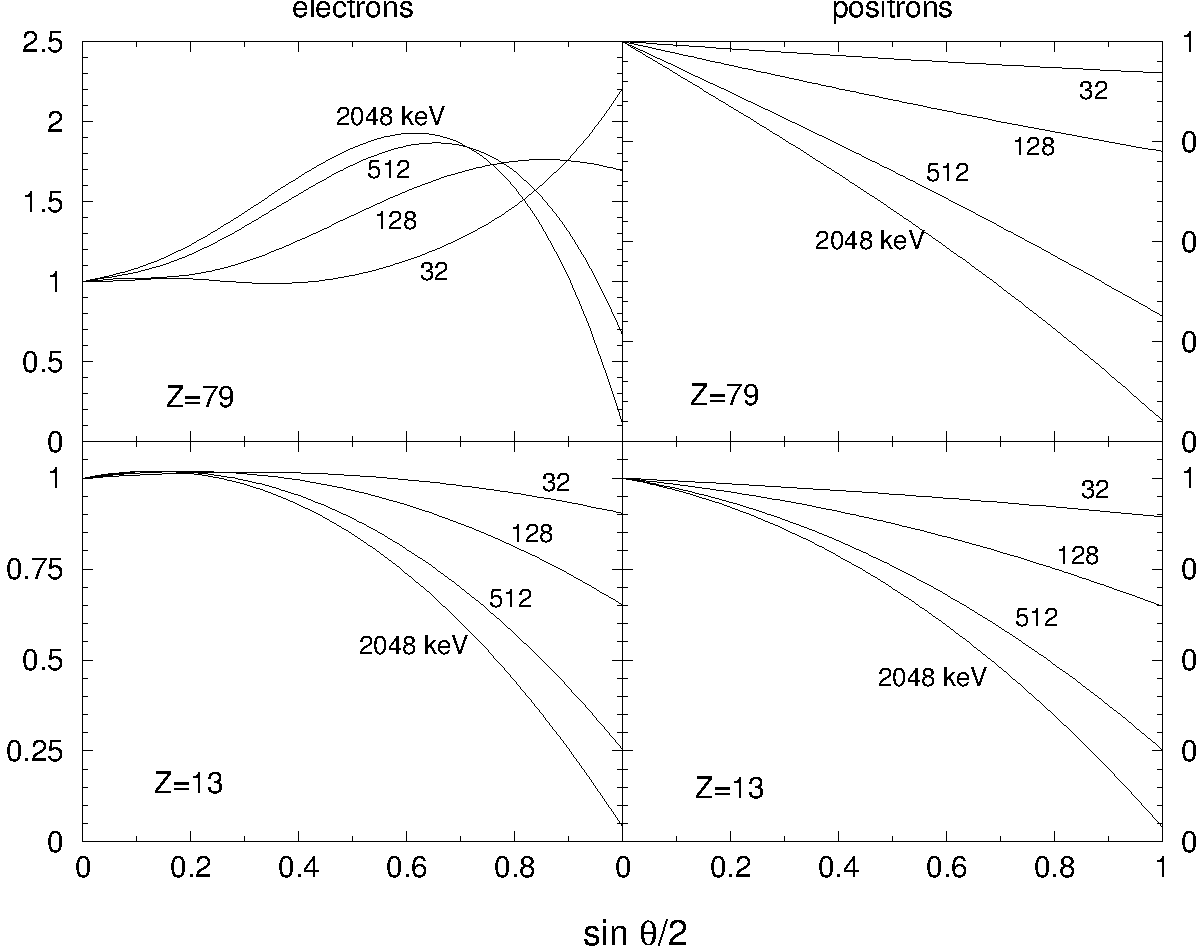
\includegraphics[height=14cm,width=14cm]{figures/mott1}
\index{Mott correction}
\caption[The Mott correction]{\label{fig_mott} The Mott correction factor
$R_{\rm mott}$ for gold and aluminum and various incident
electron and positron energies.}
\end{figure}

Berger and Wang \cite{BW89} have implemented into ETRAN (see {\em e.g.}
Ref. \cite{Se89})
the treatment of multiple
elastic scattering according to the general Mott PWA cross section,
equations \eqref{mott1} to \eqref{mott3}. They have used the code
by Riley \cite{Ri74} for the numerical solution of Eq. \eqref{mott2}
in a nuclear field screened by an electron density distribution
obtained from the multi-configuration Dirac-Fock program by
Desclaux \cite{De75}. These cross sections were later implemented
also in ITS \cite{ITSV3}. Note that ETRAN and ITS use a Class I
condensed history implementation where electron transport is
performed on  a pre-determined step-size grid. This allows
the calculation of the multiple elastic scattering distribution
(see section \ref{sec_MS}) for arbitrary complicated cross
sections for the step-size grid used with a reasonable amount
of pre-calculated data.

\index{Class II scheme!multiple scattering}
\index{Seltzer, Stephen}
The situation in a Class II code is more difficult as step-lengths
are stochastic (see section \ref{electron_general}).
Using Riley's code and Desclaux' electron
density functions, both kindly provided to us by Steve Seltzer of NIST,
we have also generated an elastic scattering data
base for all elements and energies from 1 keV to 16 MeV\footnote{
The calculation of the elastic scattering cross section from
equations \eqref{mott1} to \eqref{mott3} becomes increasingly
more difficult with increasing energy as more and more phase
shifts have to be calculated and numerical round-off errors
accumulate in the summations involved. We have modified Riley's
code to perform calculations in double precision, use more dense phase
shifts calculation grid and more accurate interpolations for
the electron density. This allowed calculations up to 16 MeV, for
even higher energies the results become numerically unstable.}.
Using this data base, we have studied the construction of a multiple
\index{multiple elastic scattering}
scattering theory but could not find a satisfactory procedure
to keep the amount of pre-calculated data required at a reasonable level.
We have therefore decided to approximate the elastic scattering
cross section as
\begin{equation}
\label{sigma_el}
{{\rm d}\sigma_{el} \over {\rm d}\mu} = {{\rm d}\sigma_{SR} \over {\rm d}\mu}
R_{\rm mott}(Z,\tau,\mu)
\end{equation}
\index{Mott correction}
where ${\rm d}\sigma_{SR}/{\rm d}\mu$ is the screened Rutherford cross
section given in Eq. \eqref{SR_1}. This approximation is known
to be accurate for energies above 1 MeV (high-$Z$ materials) or
100 keV (low-$Z$ materials) as there the spin effect correction
decouples from the screening correction \cite{BW89}. To
reproduce the average scattering at low energies we treat
the screening parameter $\eta$ as a free parameter and determine
it by numerically solving the equation
\begin{equation}
\label{fix_eta}
\int\limits_{-1}^1 {\rm d} \mu {{\rm d}\sigma_{SR} \over {\rm d}\mu}
R_{\rm mott}(Z,\tau,\mu) (1 - \mu) \equiv
\int\limits_{-1}^1 {\rm d} \mu {{\rm d}\sigma_{\rm PWA} \over {\rm d} \mu}
(1 - \mu)
\end{equation}
\index{screening parameter}
The resulting screening parameter for electrons is shown
as a function of $\beta$ for 4 different elements in
Fig. \ref{fig_eta}. In this figure $\eta$ is expressed in units
of $\eta_{\rm M}$, where
\begin{equation}
\label{eta_M}
\eta_{\rm M} = \eta_0 (1.13 + 3.76 \alpha^2 Z^2)
\end{equation}
is the screening parameter used in EGS4.
\begin{figure}[htp]
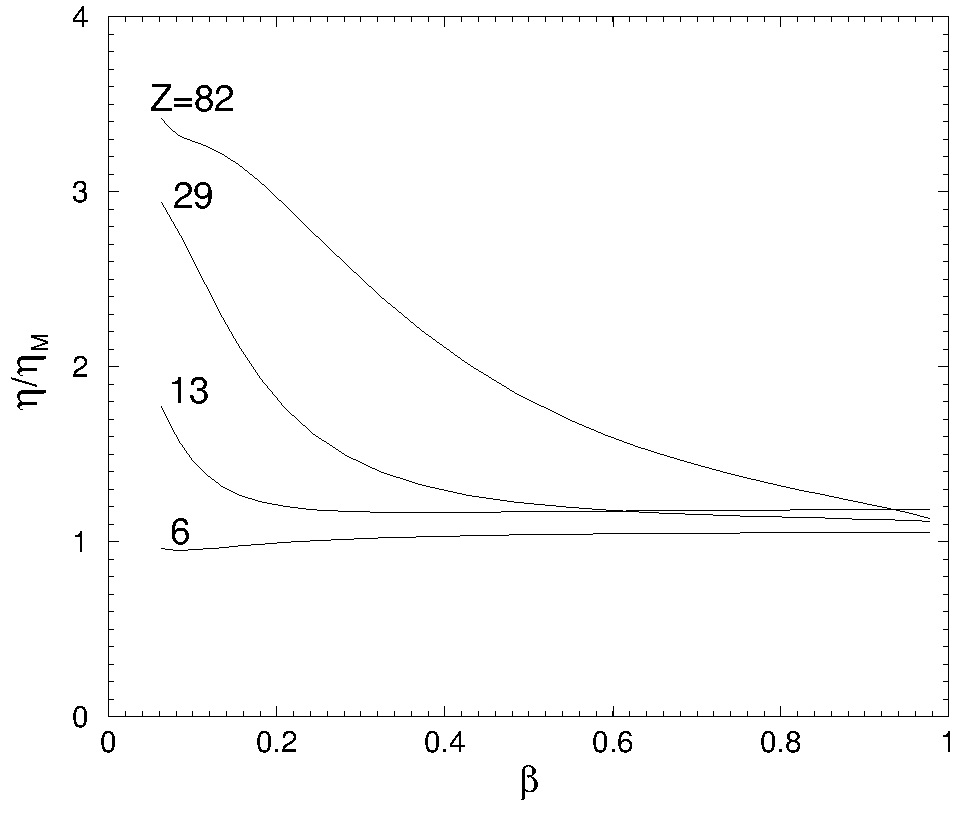
\includegraphics[height=12cm,width=12cm]{figures/eta}
\caption[Screening parameter]{\label{fig_eta} The screening parameter $\eta$,
determined from Eq. \protect\eqref{fix_eta}, in units of
$\eta_{\rm M}$, defined in Eq. \protect\eqref{eta_M}.}
\end{figure}

The elastic scattering cross section for compounds and
mixtures is expressed in a similar form as Eq. \eqref{sigma_el}
but now the Mott correction is
\begin{equation}
R_{\rm mott}(\tau,\mu) = {\sum p_i Z_i^2 R_{\rm mott}(Z_i,\tau,\mu) \over
\sum p_i Z_i^2}
\end{equation}
and the screening parameter is determined from Eq. \eqref{fix_eta} where
the partial-wave analysis cross section for the compound is
calculated from the PWA cross sections of its elements using
the independent atom approximation.

\index{angular deflections!inelastic collisions}
We can now turn to the discussion of the modifications necessary
to take into account contributions from angular deflections
due to sub-threshold processes. Various studies on this subject
are available in the literature, see {\em e.g.} \cite{Sc63,Fa54,BW89}.
We have not attempted to implement one of them, instead, we
take the simplistic point of view that the contributions
to angular deflections for all inelastic collisions, sub-threshold
and discrete, can be taken into account by replacing
$Z^2$ with $Z (Z + \xi_{0})$ in the screened Rutherford
cross section, Eq. \eqref{SR_1}. Here $\xi_0$ is an appropriate
parameter, we use by default $\xi_0=1$ but this is not a necessary
requirement. If now inelastic collisions with energy transfer
larger than $T_c$ are simulated explicitly, $\xi_0$ must
be replaced with an energy and cut-off dependent parameter $\xi(T,T_c)$
as follows \cite{Ka96c}
\begin{equation}
\xi(T,T_c) = \xi_0 \left(1 - {1 \over \bar{Z} + \xi_0}~
{g_{\rm M}(\tau,\tau_c) \over g_{\rm R}(\eta) } \right)
\end{equation}
where $\bar{Z}$ is the average atomic number of the compound
and %$g_{\rm M}(\tau,\tau_c)$ is the average angle
\newcommand{\tpr}{\tau^{\prime}}
\begin{equation}
\begin{split}
g_M(\tau,\tau_c) & =
\ln {\tau \over 2 \tau_c} + \left[1 +
{(\tau + 2)^2 \over (\tau+1)^2} \right] \ln {2 (\tau-\tau_c+2) \over \tau + 4}
\\ &-
\left[{(\tau+2)^2 \over 4} + {(\tau+2) (\tau+1/2) \over (\tau+1)^2} \right]
\ln {(\tau+4) (\tau-\tau_c) \over \tau (\tau-\tau_c+2)} \\ & +
{(\tau-2 \tau_c) (\tau+2) \over 2}
\left[{1 \over \tau-\tau_c} - {1 \over (\tau+1)^2} \right]~.
\end{split}
\end{equation}
($\tau_c = T_c/m$) and
\begin{equation}
g_{\rm R}(\eta) = (1 + 2 \eta) \left[ \ln \left(1 + \frac{1}{\eta} \right) - 2
\right]
\end{equation}

\index{SPIN\_EFFECTS}
To summarize, when spin effects are turned on in EGSnrc
({\tt SPIN\_EFFECTS = .true.}), the elastic scattering
cross section used is
\begin{equation}
\label{sigma_el1}
{{\rm d}\sigma_{\rm el} \over {\rm d}\mu} =
{2 \pi r_0^2 Z (Z + \xi(T,T_c)) \over
\beta^2 \tau (\tau + 2) }~{R_{\rm mott}(Z,T,\mu) \over (1 - \mu + 2 \eta)^2}
\end{equation}
where
\begin{itemize}
\item
The screening parameter $\eta$ is determined from the requirement
that the above cross section reproduces the average scattering
from PWA cross sections obtained via the numerical solution of
equations \eqref{mott1} to \eqref{mott3} using Hartree-Fock
electron densities. This parameter is different for electrons
and positrons
\item
The parameter $\xi(T,T_c)$ takes into account contributions
from sub-threshold inelastic collisions, it depends on energy
and the threshold energy $T_c$
\item
$R_{\rm mott}$ is the Mott correction that is the result of
the solution of the Dirac equation in the field of a bare nucleus.
\end{itemize}
All parameters necessary for the run-time interpolation
of $\eta$, $\xi$ and $R_{\rm mott}$ are initialized in
the subroutine {\tt init\_spin} which is called from
the subroutine {\tt mscati}, executed at the end of {\tt HATCH}.

Sampling of single elastic scattering events on the basis of
Eq. \eqref{sigma_el1} is performed using a rejection technique.
One uses Eq. \eqref{sample_SR} to sample the screened Rutherford
part, the $\mu$ sampled is accepted if a second random number is
less than $R_{\rm mott}/R_{\rm mott,max}$. The efficiency of
this algorithm is close to unity for low-$Z$ materials but
only close to $1/2$ for high-$Z$ materials.

\subsubsection{Multiple elastic scattering}
\label{sec_MS}
\setcounter{equation}{0}
\index{multiple elastic scattering}
\index{Goudsmit-Saunderson theory}

The multiple elastic scattering distribution for electron
transport in an infinite, homogeneous medium for a path-length
$s$, which corresponds to an energy loss $E_0 - E$, can be obtained
from Eq. \eqref{transport3} by integrating it over the position,
expanding $\Phi_0$ and the cross sections in Legendre polynomials
$P_l$ to arrive at
\begin{equation}
\Phi_0(\mu,\phi,E) = \frac{1}{2 \pi} \sum_{l=0}^\infty \left(l + \frac{1}{2}
\right) \exp( -G_l ) P_l(\mu)
\end{equation}
where $\mu$ is the cosine of the polar angle $\theta$ and the process
is considered in a frame where the electron is initially moving
along the $z$ axis. This expression was first obtained by
Goudsmit and Saunderson \cite{GS40,GS40a}. The Goudsmit-Saunderson
(GS) moments $G_l$ are given by
\begin{equation}
\label{GS_moments}
G_l = \int\limits_0^s {\rm d}s' \kappa_l(s') =  \int\limits_{E}^{E_0}
{{\rm d}E' \over L(E',E_c,k_c)} \kappa_l(E')
\end{equation}
where the $\kappa_l$ denote the moments of the elastic scattering
cross section,
\index{elastic scattering!moments}
\begin{equation}
\label{kappa_l}
\kappa_l(E) = 2 \pi
\int\limits_{-1}^1 {\rm d}\mu
\Sigma_{\rm el}'(\mu,E) \left[ 1 - P_l(\mu) \right] ~.
\end{equation}
The moments $\kappa_l$ depend on the energy and the material in
which the transport takes place, so that the
multiple elastic distribution is dependent on the energy,
path-length (or corresponding energy loss), material, and
threshold energies for discrete interactions. In a Class I
condensed history implementation one uses the total stopping
power (because discrete interaction are not explicitely modelled).
In addition, possible path-lengths are limited to the
energy-loss grid which is decided upon prior to the simulation.
These two facts allow the MS distributions to be pre-computed
and stored in the memory using a relatively small amount of
data. In a Class II implementation path-lengths are stochastic
and so a straightforward pre-calculation for all possible step-lengths
is not possible. In the past this fact has favoured use of
\index{multiple elastic scattering!small-angle approximation}
small-angle theories for the modelling of multiple elastic
scattering, {\em e.g.} the theory of \Mol~ which is used in EGS4.
The limitations of \Mol's theory have been discussed extensively
in the literature.

In EGSnrc we use an exact formulation, the multiple scattering
distributions employed being dependent on the underlying
elastic scattering cross sections (see section \ref{elastic}).

\paragraph{Multiple elastic scattering from the screened Rutherford
cross section} \hfill

\index{screened Rutherford cross section}
\index{multiple elastic scattering!based on screened Rutherford}
The multiple elastic scattering theory for the screened
Rutherford cross section employed in EGSnrc was developed
by Kawrakow and Bielajew in Ref. \cite{KB97} and later refined
by Kawrakow in Ref. \cite{Ka99a} to better take into account
energy loss.

The treatment of Ref. \cite{KB97} starts with the MS distribution
that results from the neglect of energy loss which can be written
as
\begin{equation}
2 \pi \Phi_0(\mu,\phi,E) = e^{-\lambda} \delta(1 - \mu)
+ \lambda e^{-\lambda} {1 \over \sigma_{\rm SR}}
{{\rm d} \sigma_{\rm SR}(\mu) \over {\rm d}\mu} +
\left(1 - e^{-\lambda} - \lambda e^{-\lambda} \right) F^{(2+)}_{\rm SR} (\mu)
\end{equation}
where $\lambda$ is the number of elastic free paths corresponding
to the path-length $s$,
\begin{equation}
\label{lambda}
\lambda = \Sigma_{SR} s~,
\end{equation}
and the screened Rutherford cross section
is given in Eq. \eqref{SR_1}.
The distribution $F^{(2+)}_{\rm SR}$ is the normalized multiple
scattering distribution
that results from at least two elastic collisions described by
the screened Rutherford cross section,
\index{screened Rutherford cross section}
\begin{equation}
\label{F_2plus}
\begin{split}
F^{(2+)}_{\rm SR}(\mu) & = \sum_{l=0}^\infty \left(l + \frac{1}{2} \right)
P_l(\mu) j_l^{(2+)}  \\
j_l^{(2+)} & = { \exp(-G_{l, {\rm SR}}) +
\left[ 1 + \lambda - G_{l,{\rm SR}} \right] \exp(-\lambda)
\over 1 - \exp(-\lambda) - \lambda \exp(-\lambda) }
\end{split}
\end{equation}
Here, we have put the subscript ``SR'' on the moments $G_l$
to explicitly state that they are calculated
using the screened Rutherford cross section.
Equation \eqref{F_2plus} can be put in a more tractable form
by a variable change,
\index{screened Rutherford cross section}
\begin{equation}
u = (1 + a) \left(1 - {2 a \over 1 - \mu + 2 a} \right)
\end{equation}
where the parameter $a$ is chosen such as to make $q^{(2+)}_{\rm SR}$,
\begin{equation}
q^{(2+)}_{\rm SR}(u) = F^{(2+)}_{\rm SR}(\mu)~{{\rm d} \mu \over {\rm d} u}~,
\end{equation}
``as flat as possible''. After some
straightforward manipulations one obtains \cite{KB97}
\begin{equation}
\label{a-kappa}
a = \kappa + \sqrt{\kappa^2 + \kappa}
\end{equation}
with the short hand notation
\begin{equation}
\label{kappa}
\begin{split}
\kappa & = {\langle 0\rangle - 2 \langle 1\rangle +
          \langle 2\rangle \over 4 \langle 1\rangle } \\
\langle n\rangle & =
\sum_{l=0}^\infty \left( l + {1 \over 2} \right) j_l^{(2+)}
      \sum_{m=0}^\infty \left( m + {1 \over 2} \right) j_m^{(2+)}
      \int_{-1}^1 {\rm d} \mu~ \mu^n P_l(\mu) P_m(\mu)~,
\end{split}
\end{equation}
The quantity $\omega^2 = a/\eta$ ($\eta$ is the screening parameter)
is a function of $\lambda$ and has a slight dependence
on $\eta$. In terms of simulation efficiency, it is better to
ignore the $\eta$ dependence of $\omega$ and use a fit to
the data obtained  at run time from Eq. (\ref{a-kappa},\ref{kappa}) for
$\eta \to 0$. We use
\begin{equation}
\label{fit_omega2}
\begin{split}
{\omega^2 \over \lambda + 4} & =
\begin{cases}
1.347 + t (0.209364 - t (0.45525 - t (0.50142 - 0.081234 t))) & \text{if}~
\lambda < 10, \\
-2.77164 + t (2.94874 - t (0.1535754 - 0.00552888 t)) & \text{else}
\end{cases}
\\
t & = \ln \lambda
\end{split}
\end{equation}
The dependence of the distribution $q^{(2+)}_{\rm SR}(u)$ on
$\lambda$ and $\eta$
\begin{figure}[htp]
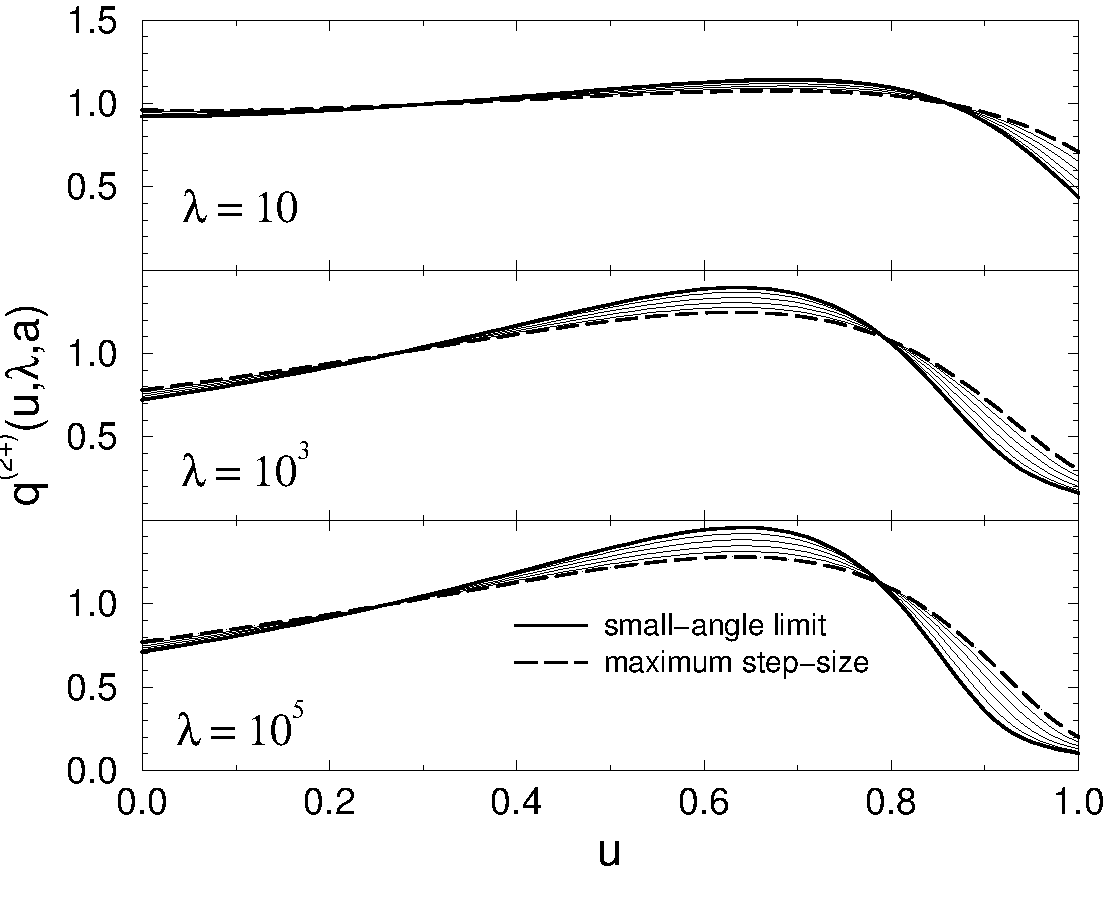
\includegraphics[height=15cm,width=15cm]{figures/q2}
\caption[The $q^{(2+)}$ surface]{\label{fig_q2}
The $q^{(2+)}_{\rm SR}$ distribution for
three step-lengths. The curve labelled ``small-angle'' limit is
the distribution for $\eta \to 0$ (infinite energy), the
curve for the maximum step-size corresponds to the
maximum step-size for condensed history steps for which the data base was
generated ($G_1 < 0.5$, see section~\ref{es_algorithm}.)}
\end{figure}
is rather weak, as can be seen in Fig. \ref{fig_q2}.
$q^{(2+)}_{\rm SR}$ can therefore be interpolated
very accurately during run time using
linear interpolation in $\ln \lambda$ and $G_{1,{\rm SR}}$
from a pre-computed table.
Here $G_{1,{\rm SR}}$ denotes the first
GS moment, see Eq. \eqref{GS_moments}, resulting
from screened Rutherford elastic scattering,
\index{screened Rutherford cross section}
\begin{equation}
\label{G1_SR}
G_{1,{\rm SR}} =
2 \lambda \eta \left[ (1 + \eta) \ln\left(1 + \frac{1}{\eta}\right) - 1
\right]
\end{equation}
The $q^{(2+)}_{\rm SR}$ data which are in a form of a 3 dimensional
alias table, are stored in the file {\tt newms.data} and read in
by subroutine {\tt init\_ms\_SR}.

\index{multiple elastic scattering!energy loss}
To take into account energy loss, one uses the multiple scattering
distribution for an ``effective'' step energy which is
determined from the requirement \cite{Ka99a}
\begin{equation}
{G_2(E_0,E) \over G_1(E_0,E)} =
{\kappa_2(E_{\rm eff}) \over \kappa_1(E_{\rm eff})}
\end{equation}
for a path-length $s_{\rm eff}$,
\begin{equation}
s_{\rm eff} = {G_1(E_0,E) \over \kappa_1(E_{\rm eff})}~.
\end{equation}
These two requirements guarantee that the first two GS moments
are exactly reproduced, and gives at the same time a very accurate
approximation for higher order GS so that the resulting
multiple scattering distribution is virtually
identical to the MS distribution calculated via numerical integration
of the moments $G_l$, see Fig. 2 of Ref. \cite{Ka99a}.

\index{screened Rutherford cross section}
For the screened Rutherford cross section the effective energy and
path-length are given by
\begin{eqnarray}
\label{E-eff}
E_{\rm eff} & = & E_0 \left[ 1 - {\epsilon \over 2} -
{\epsilon^2 \over 12 (2 - \epsilon)} \left(
{5 \tilde{\tau}^2 + 10 \tilde{\tau} + 6 \over (\tilde{\tau} + 1)
(\tilde{\tau} + 2)} + 2 b(\tilde{E}) \right) + O(\epsilon^3) \right]
\nonumber \\
s_{\rm eff} & = & s \left( 1 - {\epsilon^2 \over 3 ( 2 - \epsilon)}~
{\tilde{\tau}^4 + 4 \tilde{\tau}^3 + 7 \tilde{\tau}^2 + 6 \tilde{\tau}
+ 4 \over (\tilde{\tau} + 1)^2 (\tilde{\tau} + 2)^2} + O(\epsilon^4) \right)
\end{eqnarray}
where we have defined
\begin{equation}
\label{bE}
b(E) = {E \over C(E)}~
{{\rm d} C(E) \over {\rm d}E~}~,\quad \quad C(E) = L(E) \beta^2~,
\end{equation}
$\beta$ denoting the particle velocity in units of the speed of light.
In the above equations $\epsilon = (E_0 - E)/E$ and $\tilde{\tau} =
1/2 (E_0 + E)/m$.

\index{multiple elastic scattering!sampling of}
With all this, the algorithm for sampling multiple elastic scattering
angles is as follows:
\begin{enumerate}
\item
Calculate $s_{\rm eff}$ and $E_{\rm eff}$ from Eq. \eqref{E-eff}.
\item
Calculate $\lambda$ from Eq. \eqref{lambda} and \eqref{SR_tot},
$t = \ln \lambda$  and $\eta$ from Eq. \eqref{calc_eta}
\item
Pick a random number number $r_1$.
\item
If $r_1 < e^{-\lambda}$, then the scattering angle is zero, return
control to the calling routine
\item
Else if $r_1 < e^{-\lambda}(1 + \lambda)$, then sample $\mu$ from
the single scattering distribution according to Eq. \eqref{sample_SR},
return
control to the calling routine
\item
Else, we must sample $\mu$ from the $q^{(2+)}_{\rm SR}$ distribution.
Calculate $G_{1,{\rm SR}}$ from Eq. \eqref{G1_SR},
$\omega^2$ from Eq. \eqref{fit_omega2} and
$a = \omega^2 \eta$
\item
Determine the table look-up indices for $\ln \lambda$ and $G_{1,{\rm SR}}$
\item
Sample $u$ from the corresponding $q^{(2+)}_{\rm SR}(u)$ distribution
\item
Deliver $\mu$,
\begin{equation}
\mu = {2 a u \over 1 - u + a}
\end{equation}
\end{enumerate}


\paragraph{Multiple elastic scattering with spin effects} \hfill

\index{multiple elastic scattering!spin effects}
\index{screened Rutherford cross section}
In principle, the approach developed in Ref. \cite{KB97} could
be applied to more complicated single elastic scattering cross
sections than the screened Rutherford cross section.
We have found, however, that the direct use of this approach for
the cross section with spin effects (see section \ref{spin_elastic})
does not lead to a satisfactory interpolation accuracy. We have
therefore implemented a rejection technique for the sampling
of multiple scattering angles when {\tt SPIN\_EFFECTS = .true.}.
\index{SPIN\_EFFECTS}

We can write the multiple scattering distribution
that results from at least 2 elastic scattering processes as
\index{screened Rutherford cross section}
\begin{equation}
\label{ms_spin1}
F^{(2+)}(\lambda,\eta,Z,\mu) = F^{(2+)}_{\rm SR}(\lambda,\eta,\mu)
R(\lambda,\eta,Z,\mu)
\end{equation}
where $F^{(2+)}_{\rm SR}$ is the 2+ distribution from a
screened Rutherford cross section for a path-length corresponding
to $\lambda$ elastic mean-free paths and a screening angle $\eta$
and $R(\lambda,\eta,Z,\mu)$ is defined as
\begin{equation}
 R(\lambda,\eta,Z,\mu) = {F^{(2+)}(\lambda,\eta,Z,\mu) \over
F^{(2+)}_{\rm SR}(\lambda,\eta,\mu)}
\end{equation}
({\em i.e.} Eq. \eqref{ms_spin1} is the identity $F^{(2+)}=F^{(2+)}$).
The function $R(\lambda,\eta,Z,\mu)$ is a three dimensional
surface for each medium.
Numerical experiments show that the way which requires the minimum
amount of pre-calculated data to interpolate
the function $R(\lambda,\eta,Z,\mu)$ between pre-calculated
data is to use for each medium
\begin{itemize}
\item
Linear interpolation in the quantity $q$,
\begin{equation}
q = {2 G_{1,{\rm SR}}(\lambda,\eta) \over 1 + 2 G_{1,{\rm SR}}(\lambda,\eta)}~.
\end{equation}
Obviously $q$ can take only values between zero and unity. For
$q \to 0, R(\lambda,\eta,Z,\mu)$ converges to $R_{\rm mott}(E,Z,\mu)$,
see section \ref{spin_elastic}. For $q \to 1, R(\lambda,\eta,Z,\mu)$
goes to unity for all angles $\mu$. The rate at which the function
$R$ changes from the one limit to the other depends on the energy.
\item
Linear interpolation in $\beta^2$ for energies greater than
100 keV, linear interpolation in $\ln E$ for energies less
then 100 keV.
\item
Linear interpolation in $\sin \theta/2 = \sqrt{(1-\mu)/2}$.
\end{itemize}
The pre-calculated data are stored in separate files for
all elements in the directory {\tt spinms} and used
in subroutine {\tt init\_spin} to compute $R$ for
the media involved in the actual simulation. {\tt init\_spin}
is called from {\tt mscati} which is called from {\tt HATCH}.

The sampling algorithm is then similar to the one given at the
and of the previous section but involves an additional rejection
loop in steps 4 and 8 using $R_{\rm mott}$ or $R$ as a
rejection function\footnote{Both, $R_{\rm mott}$ and $R$ are
scaled to their maximum in the routine {\tt init\_spin}.}.
In addition, the calculation of the screening parameter
$\eta$ and the number of mean-free-paths $\lambda$ involve
additional correction factors, because both, $\eta/\eta_0$ and
the parameter $\xi$ which describe the contribution
of sub-threshold inelastic collisions to angular deflections,
are not constant, see section \ref{spin_elastic}.

\index{spin effects!measurements}
It is worth showing an example of the influence of the inclusion
of spin effects in the treatment of elastic scattering as
a conclusion of this section.
\begin{figure}[htp]
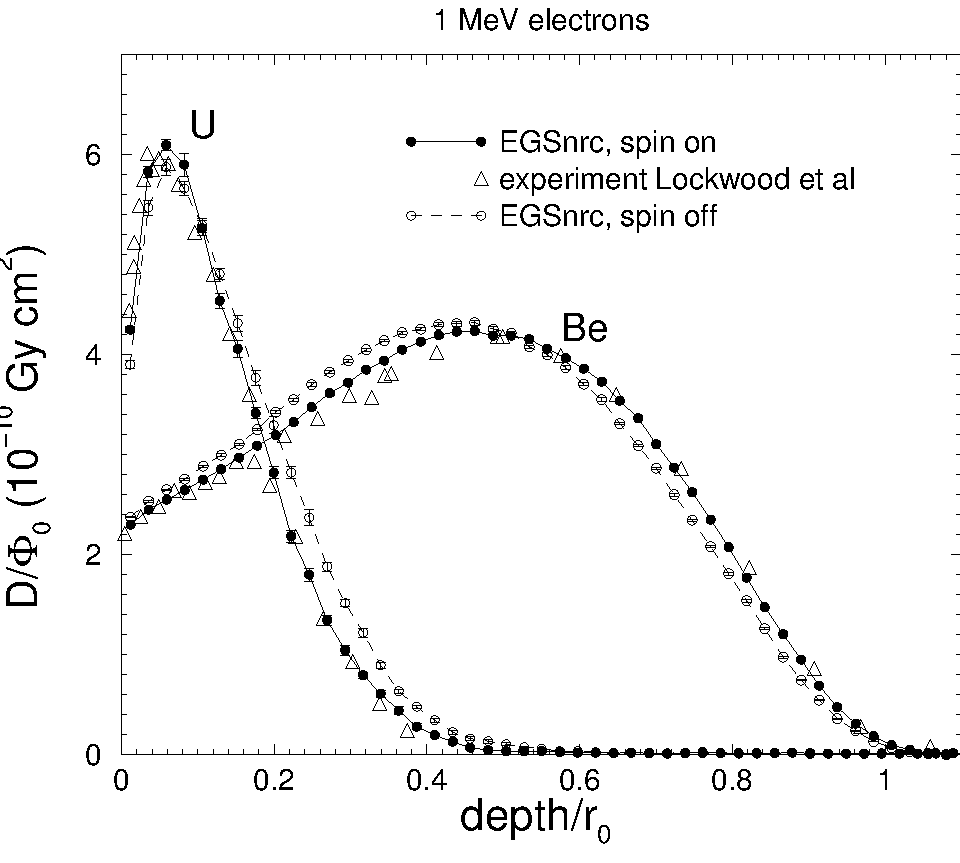
\includegraphics[height=12cm,width=12cm]{figures/dd_1MeV_Be_and_U}
\caption[Depth-dose curves in Beryllium and Uranium]{\label{dd_spin}
Depth-dose curves
for a broad parallel beam of 1 MeV electrons incident
on a Beryllium or Uranium target as a function of the CSDA range.
The experimental data are from \protect\cite{Lo80a}.}
\end{figure}
Figure \ref{dd_spin} shows a comparison of calculated depth-dose curves
in Beryllium and Uranium to measurements by Lockwood {\em et al} \cite{Lo80a}.
Both, the calculations and the measurements are absolute.
The calculations with ``spin on'' are in much better agreement
with the experiment. The effect of including spin is
to make the effective range of electrons longer for low-$Z$
materials and shorter for high-$Z$ materials. It is also
present for the energy range relevant for radiation therapy.
The reason for not seeing disagreement between EGS4 calculations
and measurements in this energy range is due to the rarity of
measurements
with precise knowledge of the incident energy. In depth-dose measurements
with a known 20 MeV electron beam incident on water, comparisons to EGS4
required using an incident beam energy of 20.3 MeV to get good
agreement\cite{Ro95}. In contrast, the calculations with EGSnrc with spin
turned on are in good
agreement with the measurements when using an incident energy of 20.0 MeV,
in agreement with the known energy.

\subsubsection{Electron-step algorithm}
\label{es_algorithm}
\setcounter{equation}{0}
\index{electron-step algorithm}

As mentioned in section \ref{electron_general},
the transport between
subsequent ``catastrophic'' collisions is described by
Eq. \eqref{transport3} with Eq. \eqref{s_vs_E} providing
the link between energy and path-length. An exact solution
of this equation is not known and so some approximate
methods are required to relate the
energy loss, the path-length, and the spatial displacement.

The simplest possible
approach one could take is to ignore deflections due
to multiple elastic scattering
during the condensed history step and
to transport the electron on a straight line along the initial
direction of motion. In order for this approach to
be accurate the CH steps must be sufficiently short so
that the straight line approach does not represent to a
severe approximation. Larsen has shown \cite{La92} that
any condensed history algorithm will converge to the correct
answer in the limit of sufficiently small step-sizes, provided
multiple elastic scattering is faithfully simulated.
However, making the step lengths very short may
cause the simulation to become extremely inefficient.
In addition, if the calculated results show step-size
dependencies, one needs to perform a careful step-size
study in order to determine when the result has
converged.

Many electron-step algorithms that attempt to make
corrections for deflections from the straight-line
approach have been proposed over the years, {\em e.g.}
\cite{Be63,BR87,Fe93,Ka96b}. A detailed discussion of these
algorithms is given in Ref. \cite{KB97a}.  In general
none of the algorithms available is accurate enough
to allow the condensed history simulation between
subsequent discrete events to be always done in a single
step. Instead, the distances between discrete collisions
is divided into smaller condensed history steps using
a procedure to determine maximum acceptable
lengths for the steps (step-size restrictions).
\index{step-size restrictions}

\index{trans\-port\_algo\-rithm}
%\index{{\tt trans\-port\_algo\-rithm}}
\index{path-length correction}
\index{lateral correlation algorithm}
\index{PRESTA}
The electron-step algorithm employed in EGSnrc depends
on the parameter {\tt trans\-port\_algo\-rithm} which
is in {\tt COMMON/ET\_Control/}. If set
to one, a slightly modified version of
PRESTA's \cite{BR87} path-length-correction (PLC)
and lateral correlation algorithm (LCA) are employed.
The PRESTA algorithm is known to underestimate
lateral deflections (deflections perpendicular to the
initial direction of motion), to underestimate
longitudinal straggling and to produce a singularity
in the distribution describing the lateral spread of electrons
in a single condensed history step \cite{Ka96b,KB97a}.
The implications on the simulation results depend on
the actual situation under investigation. At high energies,
where elastic scattering is weak, PRESTA is perhaps sufficiently
accurate. Its use for low energy applications is not
recommended. One of us has shown, for instance, that
there is up to 8\% variation of the calculated ion chamber
response subject to a $^{60}Co$ beam when using PRESTA's
transport algorithm \cite{Ka99b}.

If the parameter {\tt trans\-port\_algo\-rithm} is set to zero
(it's default value), the electron-step algorithm
developed in Ref. \cite{KB97a} and later refined in
\cite{Ka99a} is employed. This algorithm is constructed
in such a way as to reproduce up to second order spatial moments
of the fluence $\Phi_0(\vec{x},\vec{\Omega},E,t)$, which
are known from the theory of Lewis \cite{Le50} for
transport in an infinite, homogeneous medium. This algorithm
was shown to produce step-size independent results for
ion chamber simulations and backscattering \cite{Ka99a,Ka99b}, two of the
most difficult tasks for condensed history Monte Carlo codes.

For completeness, we give a brief summary of the transport
algorithms available in EGSnrc. Final positions are in a frame
where the electron is initially at the origin and moving
along the positive z-axis. Positions in the actual simulation
co-ordinate system are obtained using the appropriate
rotations and spatial translations.
\begin{itemize}
\index{PRESTA}
\item
{\tt trans\-port\_algo\-rithm = 1} (PRESTA)
\begin{equation}
\label{PRESTA}
\begin{split}
x &= r_\perp \sin \theta \cos \phi \\
y &= r_\perp \sin \theta \sin \phi \\
z &= \langle z \rangle \\
r_\perp &= \mbox{Min}\left({s \over 2},\sqrt{{s^2 - \langle z \rangle^2 \over
\sin^2 \theta}} \right)
\end{split}
\end{equation}
where $\theta$ and $\phi$ are the polar and azimuthal scattering
angles and $\langle z \rangle$ the average transport distance
in the initial direction of motion for a path-length of $s$.
In the original PRESTA implementation $\langle z \rangle$
was calculated from the theory of \Mol, we use in EGSnrc the
exact expression of Lewis \cite{Le50}, which is simply
\begin{equation}
\langle z \rangle = s~{1 - \exp(-G_1) \over G_1}
\end{equation}
if one neglects energy loss. A small correction arises
if energy loss is taken into account, it is not included
to be consistent with PRESTA where energy loss was also ignored.
\item {\tt trans\-port\_algo\-rithm = 0} (EGSnrc default) \hfill \\
The condensed history step is divided into two sub-steps and
separate multiple elastic scattering angles $\theta_1,\phi_1$ and
$\theta_2,\phi_2$ are sampled. The final scattering angle
is then determined from $\theta_1,\phi_1$,$\theta_2,\phi_2$, {\em e.g.}
\begin{equation}
\cos \theta = \cos \theta_1 \cos \theta_2 - \sin \theta_1 \sin \theta_2
\cos(\phi_1 - \phi_2)~.
\end{equation}
The final position is calculated as follows:
\begin{equation}
\label{egsnrc_algorithm}
\begin{split}
x & = s \Big[ \eta \delta \sin \theta_1 \cos \phi_1 +
\eta (1 - \delta) \sin \theta_2 ( \cos \phi_1 \cos \phi_2 -
\cos \theta_1 \sin \phi_1 \sin \phi_2 ) +
a_2 \sin \theta \cos \phi \Big] \\
y & = s \Big[ \eta \delta \sin \theta_1 \sin \phi_1 +
\eta (1 - \delta) \sin \theta_2 ( \sin \phi_1 \cos \phi_2 +
\cos \theta_1 \cos \phi_1 \sin \phi_2 ) +
a_2 \sin \theta \sin \phi \Big] \\
z & = s \Big[ a_1 + \eta \delta \cos \theta_1 +
\eta (1 - \delta) \cos \theta_2 +
a_2 \cos \theta \Big] \\
a_1 & = {1 - \eta \over 2} (1 + \alpha_1) \\
a_2 & = {1 - \eta \over 2} (1 - \alpha_1) \\
\delta & = {1 \over 2} + {\sqrt{6} \over 6} -
\left( {1 \over 4 \sqrt{6}} - \gamma {4 - \sqrt{6} \over 24 \sqrt{6}}
\right) G_1 + \alpha_2 \\
\gamma & = {G_2 \over G_1}
\end{split}
\end{equation}
Here, $\eta$ is a random number sampled from $2 \eta {\rm d} \eta$
(and not the screening parameter) and $\alpha_1$ and $\alpha_2$
are energy loss corrections derived in Ref. \cite{Ka99a},
\begin{equation}
\label{eloss_correction}
\begin{split}
\alpha_1 & = - {\kappa_1'(\tilde{E}) \over \kappa_1(\tilde{E})}~
{\Delta E \over 2} + O(\Delta E^2) \\
\alpha_2 & = \left( {\kappa_2'(\tilde{E}) \over \kappa_2(\tilde{E})}
- {\kappa_1'(\tilde{E}) \over \kappa_1(\tilde{E})} \right) {\Delta E \over
2 \sqrt{6} } + O(\Delta E^2)
\end{split}
\end{equation}
where $\Delta E$ is the sub-threshold energy loss associated
with the step, $\tilde{E}$ the average step energy and
$\kappa_1'$ and $\kappa_2'$ derivatives of the
moments $\kappa_1$ and $\kappa_2$ (see Eq. \eqref{kappa_l})
with respect to $E$.
\index{ximax}
\index{ESTEPE}
\index{$G_1$}
If elastic scattering is described by the screened Rutherford
cross section, the energy loss corrections $\alpha_1$ and
$\alpha_2$ are given by
\begin{equation}
\label{eloss_correction_SR}
\begin{split}
\alpha_1 & \approx \left( {2 + 2 \tilde{\tau} + \tilde{\tau}^2 \over
(1 + \tilde{\tau}) } - {1 + \tilde{\tau} \over
\ln(1 + 1/\tilde{\eta}) (1 + \tilde{\eta}) - 1) } \right)
{\Delta E/\tilde{E} \over  (2 + \tilde{\tau})}
\\
\alpha_2 & \approx {\Delta E/\tilde{E} \over \sqrt{6} (1 + \tilde{\tau})
(2 + \tilde{\tau}) \Big[
\ln(1 + 1/\tilde{\eta}) (1 + \tilde{\eta}) - 1) \Big]
\Big[ \ln(1 + 1/\tilde{\eta}) (1 + 2 \tilde{\eta}) - 2) \Big] }
\end{split}
\end{equation}
where $\tilde{\tau} = \tilde{E}/m$ and
$\tilde{\eta}$ is the screening parameter for
the midpoint energy $\tilde{E}$.
These equations are used in the subroutine {\tt msdist\_pII}
which implements condensed history electron transport according
to the algorithm given in Eq. \eqref{egsnrc_algorithm}.
Strictly speaking, when spin effects are ``turned on'', one
should use the energy loss corrections derived
from the moments resulting from the corresponding elastic scattering
cross section. We have left this refinment for the future because
(i) Given the fact that the corrections involve the calculation
of derivatives and that the cross sections with spin are
available only in numerical form, the implementation is more
difficult (ii) Eq. \eqref{eloss_correction_SR} does take into
account the main energy dependence of the corrections, deviations
from Eq. \eqref{eloss_correction_SR} are either higher order
in $\Delta E$ or have small coefficients.

The algorithm given in Eq. \eqref{egsnrc_algorithm} reproduces
first and second order spatial moments to better than 0.1\% for
$G_1 \le 0.5$ if energy loss is neglected ($G_1$ is defined by Eq.
\eqref{GS_moments} and is a function of pathlength, so this condition
imposes a maximum allowed step size). This accuracy
is maintained when energy loss is taken into account via
the corrections given in \eqref{eloss_correction} if
the maximum fractional energy loss per step is
restricted to 25\%. These two condensed history
step-size restrictions are controlled via the
parameters {\tt ximax} (corresponding to the maximum allowed $G_1$)
and {\tt ESTEPE} which are in {\tt COMMON/ET\_Control} and set by default
to 0.5 and 0.25.

Due to the use of the energy loss corrections derived from the
screened Rutherford cross section also for elastic scattering
with spin, in this case the deviation from the theoretical expectation
is slightly larger and exceeds 0.1\% for {\tt ESTEPE} between
0.15 and 0.2. If such a high precision is required for
your application, the simplest solution is to use step sizes
that don't exceed 20\% energy loss per step when spin is on.
\end{itemize}

%If one expands
%Eq. \eqref{transport3} in spherical harmonics,
%\begin{equation}
%\Phi_0(\vec{x},\vec{\Omega},s) = \sum\limits_{l m}
%f_{l m}(\vec{x},s) Y_{l m}(\vec{\Omega})~,
%\end{equation}
%the elastic scattering cross section in Legendre polynomials,
%and uses the addition theorem and the orthogonality, orthogona

\subsubsection{Boundary crossing algorithm}
\label{BCA}
\setcounter{equation}{0}
\index{boundary crossing algorithm}

The electron-step algorithms discussed in section
\ref{es_algorithm} are valid only for transport in
an infinite, homogeneous medium. In practical
situations one has to deal with interfaces between
different materials. If an electron is close
to an interface with another material, portions
of its curved path may be in this different material and
so the trajectory different than simulated.
In the original EGS4 version, this problem associated
with the condensed history simulation of electron
transport, which has become known as the interface artifact \cite{Bi85}, was
entirely ignored.
To address the interface artifact,
a refined boundary crossing algorithm (BCA) was
incorporated into PRESTA. According to this algorithm, the electron
is not allowed to take a step longer than $t_\perp$, $t_\perp$ being
the perpendicular distance to the closest boundary, unless
$t_\perp$ becomes smaller than $t_{min}$, a user defined
minimum step-length for boundary crossing. For $t_\perp < t_{min}$,
lateral deflections are switched off and the particle is transported,
as in the case of standard EGS4, on a straight line to the
boundary.
\index{PRESTA}

\index{boundary crossing algorithm!fluence singularity}
In a more recent paper \cite{FS95}, Foote and Smyth have demonstrated
that the approach of forcing a multiple scattering event at the
boundary causes a singularity in the simulated particle fluence.
The singularity results from the fact that there is a
non-zero probability for scattering parallel to the boundary.
Note that in real life, particles moving parallel to the boundary do
not cross it and therefore do not contribute to the planar fluence.
Although the singularity is present in any situation over a distance of the
order of $t_{min}$, it will be observed, {\em e.g.} as a dose
over-prediction, only if the
size of a scoring region is comparable to $t_{min}$ due to averaging.
One of us has developed an analytical expression for
the effect when (semi)-charged particle equilibrium is
present and has demonstrated that in the case of a small air
cavity surrounded by a dense material (ionization chamber),
the dose over-prediction may be up to 3.5\% \cite{Ka99b}.

\index{single scattering}
\index{boundary crossing algorithm!single scattering}
\index{SKINDEPTH\_FOR\_BCA}
\index{BCA\_ALGORITHM}
To overcome this problem we have implemented into EGSnrc an
exact boundary crossing algorithm, {\em i.e.} the simulation
goes over into a single elastic scattering mode whenever
an electron comes closer to a
boundary than $t_{min}$.
Whereas in the case of PRESTA one of
the criteria to determine $t_{min}$ was to assure the
applicability of \Mol's MS theory, in EGSnrc the only criterion
for $t_{min}$ is efficiency (because of the multiple scattering theory
employed which is applicable for all step-sizes). It turns out that single
scattering simulation becomes more efficient than condensed history
simulation at about
3 elastic mean free paths. This is taken as the default value
for the parameter {\tt \$SKIN\_DEPTH\_FOR\_BCA} which determines
$t_{min}$. Note that {\tt \$SKIN\_DEPTH\_FOR\_BCA} is in
elastic mean free paths and not in length units.
{\tt SKINDEPTH\_FOR\_BCA} is in {\tt COMMON/ET\_Control/}.
\index{\$SKIN\_DEPTH\_FOR\_BCA}
\index{SKINDEPTH\_FOR\_BCA}
\index{COMMON!ET\_Control}
\index{ET\_Control}

\index{PRESTA} \index{EGS4!mimic}
The investigation of Ref. \cite{Ka99b} shows that the
strength of the effect of the fluence singularity
due to forcing multiple elastic scattering events exactly
at boundaries is proportional to the first GS moment $G_1$.
At high energies $G_1$ is very small for reasonable step-sizes and
so, a single scattering simulation in the vicinity of
boundaries is potentially wasteful. Hence we decided to keep
the original PRESTA boundary crossing algorithm in EGSnrc. The selection
between exact BCA and PRESTA's BCA is made via the parameter
{\tt BCA\_ALGORITHM} which is in {\tt COMMON/ET\_Control/}.
If set to 0 (the default), exact boundary crossing is employed,
1 means PRESTA's BCA is used. If PRESTA's BCA is selected
and the parameter {\tt SKIN\_DEPTH\_FOR\_BCA} set to 0,
EGSnrc will calculate $t_{min}$ according to the procedure
in the original PRESTA implementation. It is worth noticing
that if {\tt BCA\_ALGORITHM} is set to 1 and the parameter
{\tt SKINDEPTH\_FOR\_BCA} to a very large number,
the entire simulation will run without lateral deflections
in the individual condensed history steps and so
mimic the original EGS4 behaviour. If, on the other side,
{\tt BCA\_ALGORITHM} is set to 0 and {\tt SKINDEPTH\_FOR\_BCA}
to a very large number, the entire simulation will be in
a single scattering mode. These are also the two options
available, if the geometry under investigation is
too complex to allow for the calculation of $t_\perp$.
\index{single scattering mode}
\index{BCA\_ALGORITHM}
\index{SKINDEPTH\_FOR\_BCA}
\index{emulating!EGS4/PRESTA}
\index{emulating!EGS4}

\subsubsection{Other condensed history aspects}
\label{ch_others}
\setcounter{equation}{0}

There are two additional aspects of the implementation
of the condensed history technique that deserve some
consideration:
\begin{enumerate}
\item
Calculation of path-lengths corresponding to a given
energy loss and vice versa. The two quantities are
related via Eq. \eqref{s_vs_E}.
\item
Sampling distances between discrete interactions.
Since the cross sections are energy dependent and
the energy changes via sub-threshold (continuous) energy loss,
sampling distances between discrete interactions is slightly
more complicated for electrons than for photons.
\end{enumerate}

\paragraph{Energy loss evaluation} \hfill
\index{discrete interactions!distances between}
\index{energy loss}

The energy loss $\Delta E$ due
to sub-threshold processes for
a condensed history step of length $s$ is
\begin{equation}
\label{delta_E}
\Delta E = \int\limits_0^s {\rm d}s' L(s')
\end{equation}
where the restricted stopping power is a function of $s'$
in the sense of Eq. \eqref{s_vs_E}.
Equation \eqref{delta_E} must be evaluated ``on the fly'' for
each condensed history step and so a fast and accurate
procedure is needed.
In the original
EGS4 implementation the above integral was approximated with
\begin{equation}
\Delta E \approx L(E_0) s
\end{equation}
where $E_0$ is the energy at the beginning of the step.
The PRESTA algorithm made the refinement
\index{PRESTA}
\begin{equation}
\label{eloss_presta}
\Delta E \approx L\Big(E_0 - L(E_0) s/2\Big) s
\end{equation}
The motivation for this is Euler's integration formula
\begin{equation}
\int\limits_{x - \Delta x/2}^{x + \Delta x/2} {\rm d}x' f(x')
= f(x) \Delta x + O(\Delta x^3)
\end{equation}
and so, one might expect at a first sight an $O(\Delta E^3)$ error due to
the use of Eq. \eqref{eloss_presta}. A more careful examination
of the integral reveals that Eq. \eqref{eloss_presta} still has
an $O(\Delta E^2)$ error as the original EGS4 approach (although
the coefficient of the $O(\Delta E^2)$ term is smaller).
A more accurate approach was
presented in Ref. \cite{Ka99a}, but for the official release of the
system we decided to use another approach which is simpler
but not less accurate.

In EGS4 (and also EGSnrc), a linear interpolation in $\ln E$ is
used at run time to calculate various quantities, the restricted
stopping power among them, {\em i.e.}
\begin{equation}
\label{L_interpolation}
L(E) = a_i + b_i \ln E \quad \text{for}~ E_i \le E < E_{i+1}
\end{equation}
where $E_i$ are the bin edge energies. This approach has
proven to be very accurate (and if not accurate enough,
the accuracy can always be increased by increasing the
number of interpolation bins). We now define $R_i$,
\begin{equation}
R_i = \int\limits_{E_1}^{E_i} {{\rm d} E' \over L(E')}~,
\end{equation}
where $E_1$ is the first energy in the interpolation table
(usually slightly smaller than {\tt TE}). $R_i$ is
the path-length that an electron with energy $E_i$ will
travel until local absorption if losing energy only
via sub-threshold processes (range).
\index{range}
\index{electron range}
In EGSnrc the quantities $R_i$ are stored in the array
{\tt range\_ep} which is in {\tt COMMON/ELECIN/} for each
medium. Using the $R_i$'s we can calculate the range
$R(E)$ for arbitrary energies from
\index{range\_ep} \index{COMMON!ELECIN}
\begin{equation}
\label{range}
R(E) = R_i + \int\limits_{E_i}^E {{\rm d}E' \over a_i + b_i \ln E'}
\approx R_i + {E - E_i \over L_i} \left(1 -
{b_i \over L_i}~{\epsilon \over 2} + {b_i (2 b_i + L_i) \over L_i^2}~
{\epsilon^2 \over 6} \pm \cdots \right)
\end{equation}
where $E_i$ is the lower edge energy of the bin to which $E$ belongs,
$L_i$ is a short hand notation for $L(E_i) = a_i + b \ln E_i$
and $\epsilon = E/E_i - 1$ is usually very small\footnote{{\em e.g.} for a
data set for the entire energy range of the applicability
of EGSnrc, 1 keV to 10 GeV, $\epsilon < 0.107$ using 150 interpolation
bins. Normally $\epsilon$ is much smaller.}, so that
the expansion up to second order in $\epsilon$ is sufficiently
accurate. The range of electrons is calculated according to Eq.
\eqref{range} at the beginning of each condensed history step in
EGSnrc. If now the decision is made to perform a step with
length $s$, the range of the electron at the end of the step
is $R - s$ and one can use Eq. \eqref{range} to
calculate the corresponding final step energy after finding
the bin to which the new energy belongs using the ranges
$R_i$. If, on the other side,
the step-size is determined via a given energy loss
$\Delta E$, one calculates $R(E - \Delta E)$ from
Eq. \eqref{range} and uses $R(E) - R(E - \Delta E)$  as the
corresponding step-length $s$.

The appeal of the approach described above lies in its simplicity
and generality. If one day it is decided that our understanding
of restricted stopping powers is incomplete and a change
is required, this approach will be still applicable as long
as a logarithmic interpolation is used. At this point one
should mention that the accurate knowledge of the electron range
is absolutely essential for the accurate calculation of
energy loss. Under no circumstances the variable
{\tt range} (which holds the value of $R$)
should be overwritten by the user!
\index{range}

\index{range rejection}
\index{variance reduction!range rejection}
\index{i\_do\_rr}
\index{e\_max\_rr}
An additional useful feature that results from the knowledge
of the electron range in the current material is that
electron range rejection can be applied. If the parameter
{\tt i\_do\_rr} is set to unity for the current region,
the electron energy is less than {\tt e\_max\_rr} (this
is total energy, including rest energy!) and the electron
range $R$ is less than $t_\perp$ (see section \ref{BCA}),
the simulation of the current electron is terminated and its entire energy
deposited locally.

\paragraph{Distances between discrete interactions} \hfill
\label{eloss_evaluation}

If one uses the path-length as the variable to measure
distances between discrete interactions, the path-length
$s$ to the next discrete event must be sampled from
\begin{equation}
\int\limits_0^s {\rm d} s' \Sigma^{\rm (tot)}(s') = -\ln r
\end{equation}
where $r$ is a uniformly distributed random number between
zero and unity. To avoid the numerically intensive
solution of the above equation, the so called
fictitious cross section method is employed in EGS4: an additional,
fictitious interaction is introduced, its total cross section
$\Sigma_{\rm f}(s')$ is chosen such that
\begin{equation}
\Sigma^{\rm (tot)}(s') + \Sigma_{\rm f}(s') \equiv \Sigma_0 = \text{const}~.
\end{equation}
The path-length to the next interaction, real or fictitious, is then
simply
\begin{equation}
s = -{ \ln r \over \Sigma_0 }~.
\end{equation}
Once at the interaction site, the interaction is rejected with the
probability $1 - \Sigma^{\rm (tot)}(s)/\Sigma_0$ (or, with other words,
a fictitious interaction takes place with the probability
$1 - \Sigma^{\rm (tot)}(s)/\Sigma_0$). In order this approach to work
properly, $\Sigma_0$ must be greater than $\Sigma^{\rm (tot)}(s)$ for
all $s$. Based on the observation that at high energies the
discrete interaction cross section is a monotonic increasing function
of energy, the cross section for the initial energy is used in EGS4.
This approach fails for threshold energies for delta particle
production less than about $m/7$, as pointed out by Rogers
in 1984 \cite{Ro84}. Although known for a long time, this problem
was never corrected. The modification proposed by Ma and Nahum
in 1992 \cite{MN92} is also biased, as shown in Ref. \cite{Ka99a}.
If one would attempt to employ the fictitious cross section method
using the global cross section maximum as $\Sigma_0$, the
simulation would become extremely inefficient for low values
of $T_c$ and $k_c$. This can easily be understood from
Fig. \ref{sigmas} which shows the total cross section in graphite
for two different cutoff energies.
\begin{figure}[htp]
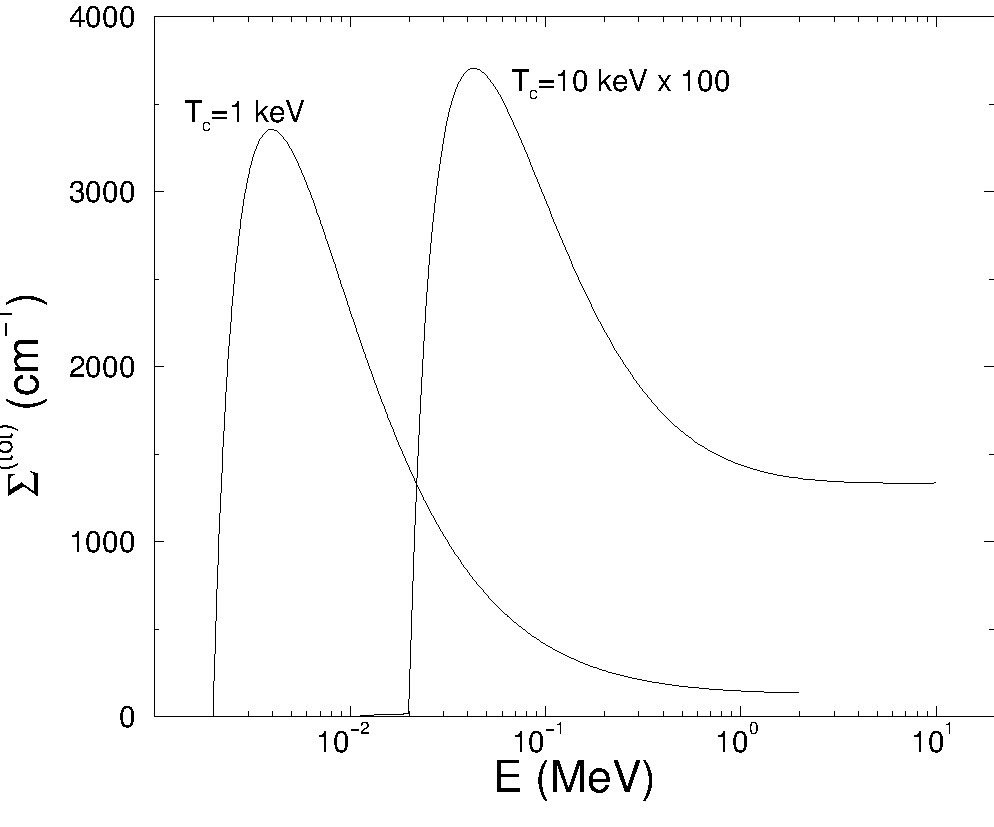
\includegraphics[height=9cm,width=9cm]{figures/cs_all}
\caption[Total discrete interaction cross sections]{\label{sigmas}
The total cross section for
discrete interactions in graphite, calculated with
$T_c = k_c = 1$~keV and $T_c = k_c = 10$~keV
(scaled by a factor of 100) as a function of kinetic energy.}
\end{figure}

In EGSnrc the distance between discrete interactions is measured
in units of the energy loss due to sub-threshold processes.
The relevant total cross section is then
$\tilde{\Sigma}^{\rm (tot)}(E) = \Sigma^{\rm (tot)}(E)/L(E)$
(see the general discussion
of the transport equation in section \ref{electron_general}).
This cross section, shown in Fig. \ref{tilde_sigma} for graphite and gold
for two different values of $T_c$ and $k_c$,
is much flatter than $\Sigma^{\rm (tot)}$
(at least for low cutoff energies)
\begin{figure}[htp]
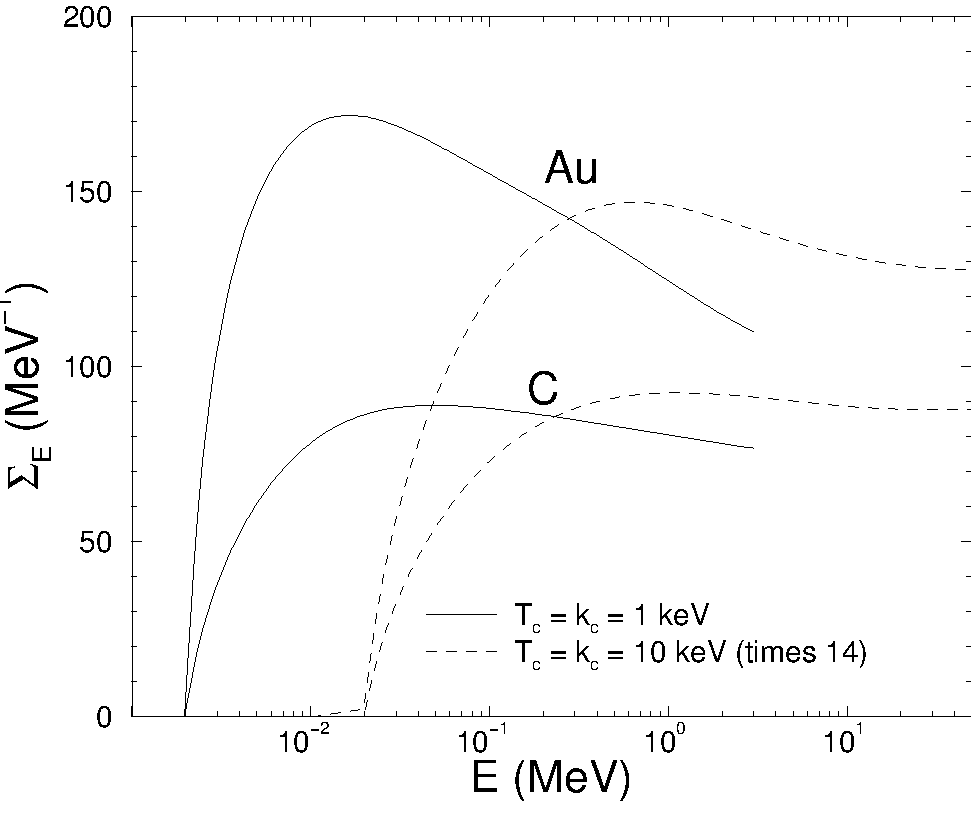
\includegraphics[height=10cm,width=10cm]{figures/cse_all}
\caption[Total cross sections per unit energy loss]{\label{tilde_sigma}
The total cross section
per unit energy loss, $\tilde{\Sigma}^{\rm (tot)}(E)$, for
discrete interactions in graphite and gold, calculated with
$T_c = k_c = 1$~keV and $T_c = k_c = 10$~keV
(scaled with a factor of 14 for better visibility)
as a function of kinetic energy.}
\end{figure}
and has a single maximum. This maximum is determined after
the PEGS data becomes available and is used at run time to
sample energy losses between discrete interactions.
This saves the necessity of evaluating the cross section
at the beginning of each discrete interaction loop
(the {\tt TSTEP LOOP}) in subroutine {\tt ELECTR}.
The procedure described above
is then used to compute the corresponding path-length.

\paragraph{Transport in electromagnetic fields} \hfill
\label{EMF_macros_algorithm}

Transport of charged particles through matter under the influence of electric and magnetic fields is now possible
using the approach proposed by Bielajew\cite{Bi89a}. In this approach, charged particles are forced
to take small enough steps so that the external fields do not change significantly, and energy losses as well
as angular deflections are negligible. Under these assumptions the effect of the electromagnetic field can
be superimposed upon the field-free transport, and the final direction calculated to first order as

\begin{equation}
\Delta\vec{u} = \Delta\vec{u}_{ms,ret} + \Delta\vec{u}_{em}
\end{equation}
where $\Delta\vec{u}_{ms,ret}$ is the angular deflection due to elastic and inelastic scattering which
can be calculated using EGSnrc's electron transport algorithm, and $\Delta\vec{u}_{em}$ is the angular
deflection due to the electromagnetic field, which, to first order, can be obtained from

\begin{equation}
\label{uchange_emf}
    \Delta\vec{u}_{em} = \frac{q \cdot s}{m_0 \gamma v^2_0} \left[\vec{E}_0 - \vec{u}_0(\vec{u}_0\cdot \vec{E}_0) + \vec{v}_0 \times \vec{B}_0\right].
\end{equation}

The final position can be obtained using

\begin{equation}
    \vec{x}_f = \vec{x}_0 + \vec{u}_0 s + \frac{s}{2} \left(\Delta\vec{u}_{ms,ret} + \Delta\vec{u}_{em}\right).
\end{equation}

In the current implementation, lateral displacement due to the Lorentz force is ignored,
and only a condensed history (CH) step $s$ is taken along $\vec{u}_0$ using EGSnrc's electron
transport algorithm. This simplification relies on the assumption that accounting only for
the change in direction due to the Lorentz force is accurate enough when using very small steps.

There are several criteria to restrict the step size based on energy loss, change
in the electromagnetic field and change in particle direction. In the case of a static
$\vec{B}$ field ($\vec{E}$ = 0, $\vec{B}$ = $\vec{B}_0$) only the restriction of small changes
in the particle direction is relevant. According to Eq.(\ref{uchange_emf}), $|\Delta\vec{u}_{em}|$
should only be allowed to take a value $\delta \ll 1$ from where the restricted step size follows as
\begin{equation}
\label{uchange_restriction}
  s = \delta \cdot \frac{E_o \gamma_0 \beta^2}{q\left|\vec{v}_0 \times \vec{B}_0\right|} = \delta \cdot r_g
\end{equation}
the quantity $r_g$ is the well known gyroradius of the particle's trajectory. A value of $\delta$ = 0.02
was used to reproduce the analytical trajectory of electrons in vacuum in reference \cite{Bi89a}.
For more details on the implementation of this algorithm the reader is encouraged to read the very detailed
chapter on this topic by Bielajew\cite{Bi89a}. For instructions on how to enable transport under electromagnetic
fields please refer to section \ref{EMF_macros_implementation}.

\newpage


%%%%%%%%%%%%%%%%%%%%%%%%%%%%%%%%%%%%%%%%%%%%%%%%%%%%%%%%%%%%%%%%%%%%%%%%

%		EGSnrc User Manual

%%%%%%%%%%%%%%%%%%%%%%%%%%%%%%%%%%%%%%%%%%%%%%%%%%%%%%%%%%%%%%%%%%%%%%%%

%\mbox{}\newpage
\renewcommand{\leftmark}{{3: EGSnrc Reference Manual}}
\typeout{Starting ``EGSnrc Reference Manual''  Should be odd page}
%\renewcommand{\rightmark}{{EGSnrc Reference Manual}}

%%%%%%%%%%%%%%%%%%%%%%%%%%%%%%%%%%%%%%%%%%%%%%%%%%%%%%%%%%%%%%%%%%%%%%%%%%%%%%%
%
%  EGSnrc manual: changes from EGS4
%  Copyright (C) 2015 National Research Council Canada
%
%  This file is part of EGSnrc.
%
%  EGSnrc is free software: you can redistribute it and/or modify it under
%  the terms of the GNU Affero General Public License as published by the
%  Free Software Foundation, either version 3 of the License, or (at your
%  option) any later version.
%
%  EGSnrc is distributed in the hope that it will be useful, but WITHOUT ANY
%  WARRANTY; without even the implied warranty of MERCHANTABILITY or FITNESS
%  FOR A PARTICULAR PURPOSE.  See the GNU Affero General Public License for
%  more details.
%
%  You should have received a copy of the GNU Affero General Public License
%  along with EGSnrc. If not, see <http://www.gnu.org/licenses/>.
%
%%%%%%%%%%%%%%%%%%%%%%%%%%%%%%%%%%%%%%%%%%%%%%%%%%%%%%%%%%%%%%%%%%%%%%%%%%%%%%%
%
%  Author:          Iwan Kawrakow, 2003
%
%  Contributors:    Blake Walters
%                   Frederic Tessier
%                   Ernesto Mainegra-Hing
%
%%%%%%%%%%%%%%%%%%%%%%%%%%%%%%%%%%%%%%%%%%%%%%%%%%%%%%%%%%%%%%%%%%%%%%%%%%%%%%%


% Replace line with fixed date with the one below when commiting
% Beware: Using the macro below conflicts between CVS and latex!!!
% \lfoot[{\sffamily {\leftmark}}]{{\small Last edited $Date: 2013/01/04 14:38:47 $
\lfoot[{\sffamily {\leftmark}}]{{\small Last edited 2011/03/09 19:35:20
}}
\newpage

\section{EGSnrc Reference Manual}
\label{ERM}

\subsection{Introduction}

This section is based on Appendix 2 of SLAC-265\cite{Ne85} but
substantially updated and changed to represent the EGSnrc system rather
than EGS4. There have been minor modifications to reflect the EGSnrcMP
environment but these are described more fully in PIRS-877\cite{Ka03}.

\subsubsection{Use of Mortran3}
\index{Mortran3}

Starting with EGS2, the EGS Code System has been written in an extended
Fortran language known as Mortran\cite{Co83}. Section~\ref{UGM3} (page
~\pageref{UGM3}) presents a
brief overview of the elements of Mortran3 which are needed for users of
EGS.

Mortran is a very powerful pre-processor which was ahead of its time back
in the 70's and 80's.  Today many of its features are available in other
languages. Nonetheless we have continued to use Mortran3 because there
are so many user codes available in Mortran3 that it makes no sense to
abandon it.  It is also a very structured language which allows for easy
in-line documentation.


      Although there might be some resistance by users of EGS
 to learn another language, we would like to point out two facts:
\begin{itemize}
      \item   The Mortran language (excluding macros) is trivial
            to learn by those who program in Fortran.

      \item   EGS can be set-up and run by writing entirely in
            Fortran or some other language should the user so desire.
\end{itemize}

 We would encourage EGS users not to do the latter, however, for this
would truly defeat the real purpose for using Mortran---namely, the
macro facility.


\subsection{ General Description of Implementation}
\index{overview of code system}
\index{general description of code system}

The EGS code itself consists of two User-Callable subroutines, {\tt HATCH}
and {\tt SHOWER}, which in turn call the other subroutines in the EGS
code, some of which call three User- written subroutines, {\tt HOWFAR},
{\tt HOWNEAR} and {\tt AUSGAB}.  This is best illustrated with the aid
of Fig.~\ref{fig_egsnrc_structure}

\begin{figure}[hbtp]
\index{schematic of code system}
   \begin{center}
   \leavevmode
   \mbox{}\hspace{-1mm}
   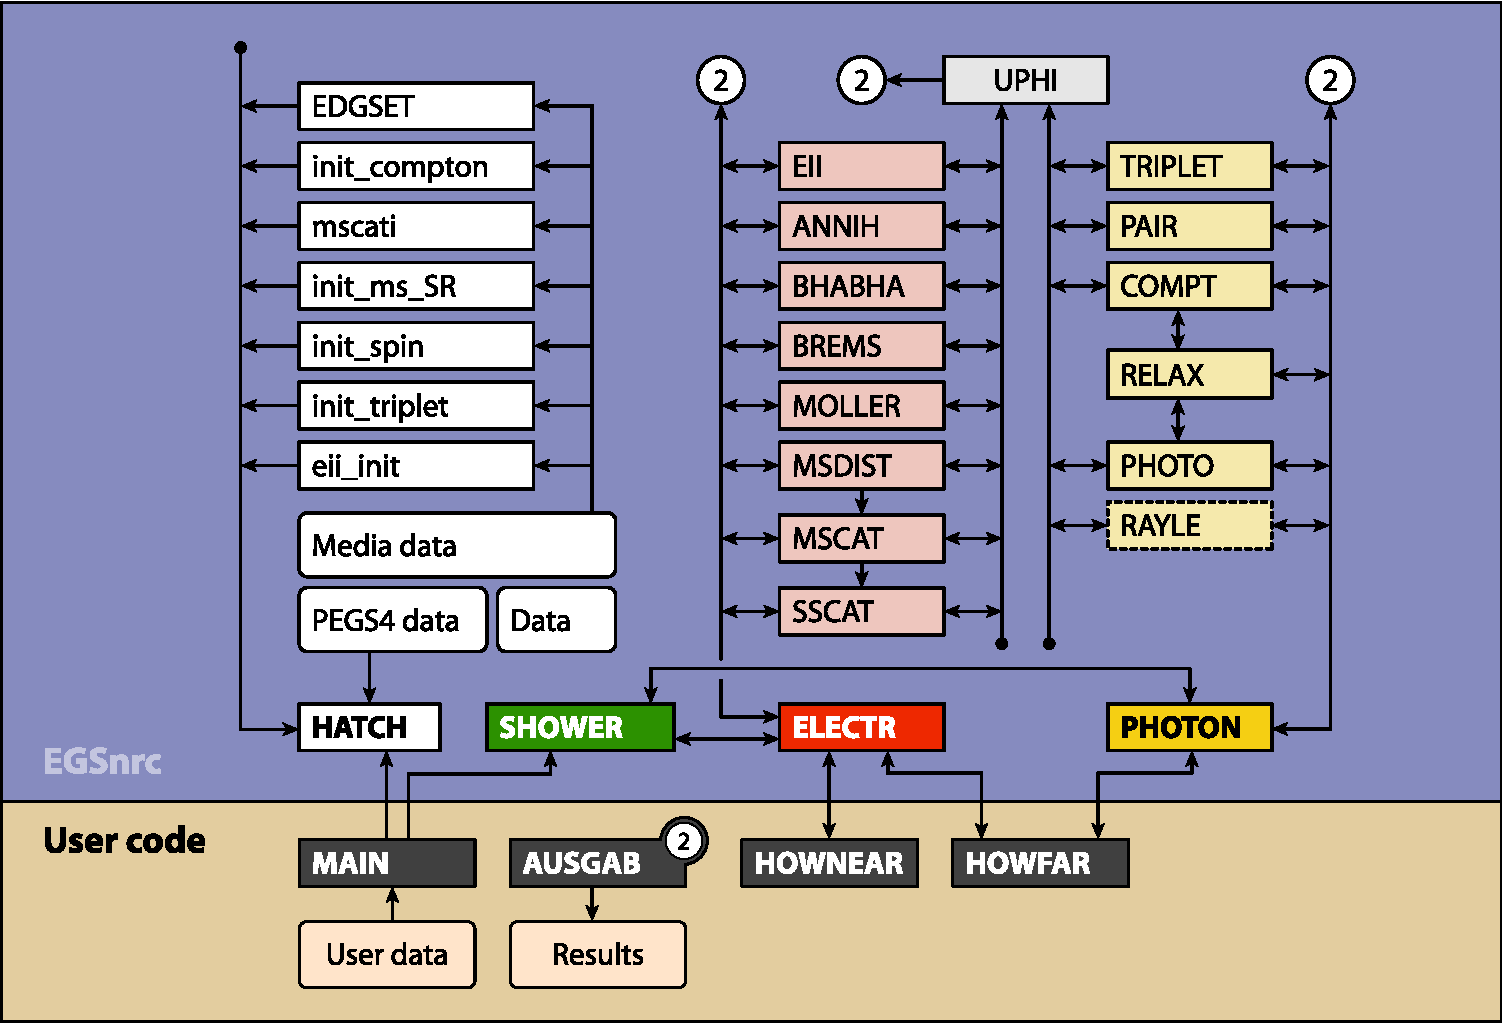
\includegraphics[width=16cm]{figures/egs-diagram}
   \end{center}
   \caption{The structure of the EGSnrc code system when used with a
user-code.}
   \label{fig_egsnrc_structure}
\end{figure}

To use EGS the user must write a ``User Code."  This consists of a
MAIN program and the subroutines {\tt HOWFAR}, {\tt HOWNEAR} and {\tt
AUSGAB}, the latter three determining the geometry and output (scoring),
respectively.  Additional auxiliary subprograms might be included in the
User Code to facilitate matters.  The user can communicate with EGS by
means of various {\tt COMMON} variables.  Usually MAIN will perform
any initialisation needed for the geometry routines, {\tt HOWFAR}
and {\tt HOWNEAR}, and sets the values of certain EGS {\tt COMMON}
variables which specify such things as names of the media to be used,
the desired cutoff energies, and the distance unit to be used (e.g.,
inches, centimeters, radiation lengths, etc.).  MAIN then calls the
{\tt HATCH} subroutine which ``hatches EGS" by doing necessary once-only
initialisation and by reading material data for the media from a data set
that had been previously created by PEGS.  This initialisation completed,
MAIN may then call {\tt SHOWER} when desired.  Each call to {\tt SHOWER}
results in the generation of one history (often referred to as a ``case").
The arguments to {\tt SHOWER} specify the parameters of the incident
particle initiating the cascade.

In addition, macro definitions can be included in MAIN in order to control
or over-ride various functions in EGS as well as in the User-Written
codes.

\index{defaults}
In EGSnrc there are many new options compared to EGS4.  The system
defaults to a set of options which will do the most complete and accurate
simulation that EGSnrc is capable of. In some cases this will imply
overkill and a reduction in efficiency with no gain in accuracy (e.g.
including atomic relaxation or bound Compton scattering for high energy
photon calculations). The user has the ability to switch things on or off
by setting various  flags.  So, eg, one could decide to run a calculation
which is nearly equivalent to using the EGS4/PRESTA electron transport
algorithm (see section~\ref{mimic}). Similarly one can choose to model
Klein Nishina Compton scattering instead of bound compton scattering by
setting a flag.

One other class of new features in EGSnrc is the implementation within the
code itself of several variance reduction techniques (range rejection and
bremsstrahlung splitting being the main two) since by doing so, a much more
efficient implementation is allowed. The user can, of course, completely
ignore these features if so desired.


      In summary, the user communicates with EGS by means of:
\begin{description}
\item[Subroutines]\mbox{}
\begin{itemize}
\item HATCH  --- to establish media data

\item SHOWER --- to initiate the cascade

\item HOWFAR\& HOWNEAR --- to specify the geometry

\item AUSGAB --- to score and output the results and to control variance
reduction

\end{itemize}

\item[COMMON blocks]  by changing values of variables

\item[Macro definitions] --- re-definition of pre-defined features.
\end{description}

To reiterate, we shall refer to the MAIN/HOWFAR/AUSGAB combination
(plus auxiliary subprograms and macros) as the User Code.  The following
sections discuss these things in greater detail.

\clearpage

%\newpage
\subsection{ The COMMON Blocks}

\label{common_blocks} \index{COMMON BLOCKS}
Listed here are the {\tt COMMON} blocks relevant to the user (and
relevant variables contained in them) with a brief description of their
functions.  Their usage will be discussed in more detail in subsequent
sections.  The easiest way to declare any of the {\tt COMMON} blocks is with
the {\tt COMIN} macro.  For example, {\tt COMIN/STACK,BOUNDS/;} will automatically
expand to the correct {\tt COMMON/STACK/;} and {\tt COMMON/BOUNDS/;} forms.

Note that EGSnrc is, by default, coded completely using IMPLICIT NONE. This
means that all parameters in {\tt COMMON} are all explicitly typed. See
section~\ref{implicit_none}  for more info.

\begin{table}[htb]
   \index{BOUNDS} \index{COMMON!BOUNDS} \index{ECUT}
   \index{PCUT} \index{VACDST} \index{EGS-VARIANCE-REDUCTION}
   \index{COMMON!EGS-VARIANCE-REDUCTION} \index{e\_max\_rr} \index{i\_do\_rr}
   \index{i\_play\_RR} \index{i\_survived\_RR} \index{prob\_RR}
   \index{n\_RR\_warning} \index{nbr\_split} \index{bremsstrahlung!splitting}
   \index{Russian Roulette} \index{range rejection}
   \index{bound Compton scattering}

\typeout{starting common BOUNDS table }


\begin{center}
\caption{Table describing the EGSnrc {\tt COMMON}s which are accessible to the
User.
\label{tab_commons}
}
\begin{tabular}{ l l   p{105mm}l  |}
\hline
Common & Variable & Description \\
Block &&\\
\hline
&&\\
{\bfseries BOUNDS} & ECUT &Array of regions' charged particle
                            cutoff energies(total) in MeV.\\
       & PCUT &Array of regions' photon cutoff
                            energies in MeV.\\
       & VACDST  &   Distance to transport in vacuum (default=1.E8).\\
&&\\
\hline
&&\\
\multicolumn{3}{l}{{\bfseries EGS-VARIANCE-REDUCTION}}\\
	&e\_max\_rr &real array (\$MXREG) of maximum total energies at which
                     to do range rejection if i\_do\_rr is set\\
	&i\_do\_rr &integer array (\$MXREG) of flags for range rejection
                    in each region. ~~~~0$\Rightarrow$ not done (default);
                      ~~~~1$\Rightarrow$ is done.\\
&&\\
	& i\_play\_RR & flag specifying if Russian Roulette played on a
                        global basis\\
        & i\_survived\_RR & an integer flag set every time Russian Roulette
is played. If all the particles survive, it is set to 0 (which is the default
if not played at all). It is set to n if n particles were eliminated via
Russian Roulette on this interaction. It is 0 if a bound compton event is
rejected.\\
&&\\
	& prob\_RR & probability of survival if playing Russian Roulette\\
	& n\_RR\_warning & an internal counter to mark how often Russian
	Roulette is asked for with prob\_RR $\le$ 0.0. A warning is printed
       for the first \$MAX-RR-WARNING times (default 50).\\
&&\\
	&nbr\_split& For nbr\_split $>$1, nbr\_split brems photons are
sampled {every time} there is a brem interaction. The weight is reduced by
1/nbr\_split. Default value is 1.0.  If set to zero, no brem is generated
and the electron loses no energy.\\
%&&\\
\hline
    \end{tabular}
    \end{center}
    \mbox{}\hfill (cont ...)\\
    \end{table}
    \clearpage

\begin{table}[htb]
   \index{EPCONT} \index{COMMON!EPCONT} \index{EDEP} \index{TSTEP}
   \index{TUSTEP} \index{USTEP} \index{VSTEP} \index{IDISC} \index{IROLD}
   \index{IRNEW} \index{EOLD} \index{RHOF} \index{ENEW} \index{BETA2}
   \index{IAUSFL} \index{EKE} \index{ELKE} \index{GLE} \index{E\_RANGE}

\typeout{starting next common EPCONT table }
    \begin{center}
    EGSnrc COMMONs which are accessible to the User -continued\vspace*{3mm}
    \begin{tabular}{ l  l   p{105mm}l  |}
    \hline
    Common & Variable & Description \\
    Block &&\\
    \hline
&&\\
{\bfseries EPCONT}  & EDEP & Energy deposited in MeV (Double
                            Precision).\\
        & TSTEP  & Distance to next interaction (cm)\\
        & TUSTEP  & Total (curved) step length requested before check with
		geometry.\\
	& USTEP	& straight step length calculated from TUSTEP.\\
        & TVSTEP & Actual total (curved) step length to be transported.\\
	& VSTEP	& actual straight step length after truncation by geometry.\\
        & IDISC  & User discard request flag (to be set in {\tt HOWFAR}).
                   IDISC $>$ 0 means user requests immediate discard,
                   IDISC $<$ 0 means user requests discard after completion
                   of transport, and IDISC=0 (default) means no user
                   discard requested. IDISC=99 or $-$99 means generate
		   annihilation photons when positron is discarded.\\
         &IROLD  &Index of previous region.\\
         & IRNEW  & Index of new region.\\
         & RHOF   & Value of density correction (default=1) (i.e. ratio
                    of real density to that of dataset.\\
         & EOLD   &  Charged particle (total) energy
                            at beginning of step in MeV.\\
           & ENEW   & Charged particle (total) energy
                            at end of step in MeV.\\
           %& BETA2 & Beta squared for present particle.
                  %          (Note: BETA is not included).\\

           & IAUSFL & Array(35) of flags for turning on
                   various calls to {\tt AUSGAB}. See table~\ref{tab_iausflg_other}\\
           & EKE   & Electron kinetic energy in MeV.\\
           & ELKE  & Natural logarithm of EKE (this is not available for
                     a step in vacuum).\\
           & GLE   & Natural logarithm of photon energy.\\
           & E\_RANGE & For electron {\tt IARG}=0  steps, this is the range of the
electron in the current units (see section~\ref{range_rejection}).\\
           & x[y][z]\_final & position at end of step \\
           & u[v][w]\_final & direction at end of step (only used for electrons)\\
&&\\
\hline
    \end{tabular}
    Note: the variable BETA2 is no longer available.\\
    \end{center}
    \mbox{}\hfill (cont ...)\\
    \end{table}

\clearpage

  \begin{table}[htb]
   \index{ET-Control} \index{COMMON!ET-Control} \index{SMAXIR}
   \index{ESTEPE} \index{XIMAX} \index{SKINDEPTH\_FOR\_BCA}
   \index{TRANSPORT\_ALGORITHM} \index{SPIN\_EFFECTS} \index{EGS4}
   \typeout{starting next common ET-Control table }
   \index{BCA\_ALGORITHM}
    \begin{center}
    EGSnrc COMMONs which are accessible to the User -contnued\vspace*{3mm}
    \begin{tabular}{ l  l   p{105mm}l  |}
    \hline
    Common & Variable & Description \\
    Block &&\\
    \hline
    &&\\
    \multicolumn{2}{l}{{\bfseries ET-Control}}  &  Electron Transport Control.\\
    &&\\
	&SMAXIR	&array(\$MXREG) defining upper limit on step size in each
		region (in whatever units defined by DUNIT).(default=1.E10).\\
    &&\\
	&ESTEPE	&global energy loss constraint.(default=0.25).\\
    &&\\
	&XIMAX	&max. first GS moment per step (roughly half the average
                MS angle squared.(default 0.5).\\
    &&\\
	&SKINDEPTH      & distance from a boundary (in elastic MFP) at which to\\
	&  ~~~\_FOR\_BCA& switch to one of the boundary crossing
		  algorithms(BCAs).(default 3).  If set 0 by the user
                  initially and BCA\_ALGORITHM = 1, then the code assigns
                  a value consistent with
                  BLCMIN in PRESTA-I, otherwise it is 3.0.\\
    &&\\
	&TRANSPORT& integer flag telling which transport algorithm to use.\\
 	& \_ALGORITHM	& 0$\Rightarrow$ PRESTA-II; 1$\Rightarrow$
                    PRESTA-I.(default 0).\\
    &&\\
	&BCA	&integer flag telling which BCA to use. \\
	&\_ALGORITHM  & 0$\Rightarrow$ use exact(single scattering) algorithm
                         within SKINDEPTH\_FOR\_BCA of a boundary\\

        &            &  1$\Rightarrow$ use multiple scattering but with
                  no lateral deflections within SKINDEPTH\_FOR\_BCA of a
                  boundary.  Default is  0.\\
    &&\\
      	&SPIN &logical variable, {\tt .true.}$\Rightarrow$ use single \&
                multiple scattering\\
	&\_EFFECTS	& theories which include relativistic spin
               effects; {\tt .false.}
		$\Rightarrow$ use single and multiple scattering theories
                based on Rutherford scattering. (default {\tt .true.})\\
%to be closer to EGS4).\\
	&&\\
   \hline
   \end{tabular}
   \end{center}
\end{table}

\clearpage

\begin{table}[htb]
    \index{MEDIA} \index{COMMON!MEDIA} \index{NMED} \index{IRAYLM} \index{RLC}
    \index{RLDU} \index{RHO}
    \index{MISC} \index{COMMON!MISC} \index{MED} \index{DUNIT} \index{KMPI}
    \index{KMPO} \index{RHOR} \index{NOSCAT} \index{IRAYLR}
    \index{RANDOM} \index{COMMON!RANDOM} \index{IXX} \index{JXX}
    \index{random number generators!seeds} \index{RANMAR} \index{RANLUX}

\typeout{****start Common MEDIA}
    \begin{center}
    EGSnrc COMMONs which are accessible to the User (cont)\vspace*{2mm}
    \begin{tabular}{ l  l   p{105mm}l  |}
    \hline
    Common & Variable & Description \\
    Block &&\\
    \hline
&&\\
{\bfseries MEDIA}	& MEDIA	&array(24,\$MXMED)  of media names.\\
	& NMED	& Number of media being used
                            (default=1).\\
          & IRAYLM & Array(\$MXMED) of flags for turning on (=1)
                            coherent (Rayleigh) scattering in
                            various media.  Set in {\tt HATCH} based
                            on values of IRAYLR.  \\
          & RLC   & Array(\$MXMED) containing radiation
                            lengths of the media in cm.  \\
	& RLDU  &  Array(\$MXMED) containing radiation
                            lengths of the media in distance
                            units established by DUNIT.\\
	&RHO	& Array(\$MXMED) containing density of the
                            media in g/cm**3.\\
        &MGE    & Array(\$MXMED) number of photon mapped energy intervals for
                  a given medium.\\
        &MEKE   & Array(\$MXMED) nuber of electron mapped energy intervals for
                  a given medium.\\
       &comp\_xsections & character*16 variable holding the name of the file\\
       && containing user-supplied Compton cross section data.\\
       &&  Full name of the file is\\
       && {\tt \$HEN\_HOUSE/data/comp\_xsections\_compton.data}.\\
       && Only used if {\tt IBCMP}=2 (bound Compton, no doppler effect).\\
&&\\
\hline
&&\\
{\bfseries MISC$^*$}	& MED	&Array(\$MXREG) containing medium index for
                            each region.\\
	& DUNIT	&The distance unit to be used.
                            DUNIT=1 (default) establishes all
                            distances in cm; whereas,
                            DUNIT=2.54 establishes all
                            distances in inches.\\
	&KMPI	&Fortran unit number (default=12)
                            from which to read material data.\\
	&KMPO	&Fortran unit number (default=8) on
                            which to ``echo" material data (e.g.,
                            printed output, ``dummy" output, etc.).\\
	&RHOR	&Array(\$MXREG) containing the density for each region (g/cm**3).
		If this is different than the default density for the medium
		for that region, the cross sections and stopping powers (with
		the exception of the density effect) are scaled appropriately.\\
	%&NOSCAT&Number of times multiple scattering has been bypassed in
        %       subroutine MSCAT (initialized to 0 in BLOCK DATA). This
	%       applies only if PRESTA-I or EGS4 options being used since
        %       it is never turned off in default EGSnrc.\\
	&IRAYLR	&Array(\$MXREG) of flags for turning on (=1)
                            coherent (Rayleigh) scattering in
                            various regions (default=0$\Rightarrow$ off).\\
&&\\
\hline
\multicolumn{3}{c}{$^*$ NOSCAT is no longer available since there is
scattering on all steps.}\\
&&\\
%this common block is now found in ranmar.macros and ranlux.macros and,
%moreover, does not include ixx, jxx
%{\bfseries RANDOM}
%	&IXX,JXX & When using the RANLUX random number generator, the user
%does not pass anything via this {\tt COMIN}. When using RANMAR, IXX and JXX
%are passed. Initially random number seeds, these
%become pointers once the generator is initialized. 0$<$IXX$<=$31328 and 0$<$JXX$<=$30081.\\
\hline
    \end{tabular}
    \end{center}
    \mbox{}\hfill (cont ...)\\
    \end{table}
    \clearpage



\begin{table}[htb]

   \index{STACK} \index{COMMON!STACK} \index{E} \index{X,Y,Z} \index{U,V,W}
   \index{DNEAR} \index{WT} \index{IQ} \index{IR} \index{NP} \index{NPold}
   \index{LATCH} \index{LATCHI}


   \index{THRESH} \index{COMMON!THRESH} \index{RMT2} \index{RMSQ} \index{AP}
   \index{UP} \index{AE} \index{UE} \index{TE} \index{THMOLL} \index{\$MXMED}
   \index{\$MXSTACK} \index{variance reduction}

\typeout{****start COMMON STACK}

    \begin{center}
    EGSnrc COMMONs which are accessible to the User (cont).
    \begin{tabular}{ l  l   p{105mm}l  |}
    \hline
    Common & Variable & Description \\
    Block &&\\
    \hline
&&\\
{\bfseries STACK}	&	&Note: This COMMON block contains the
                            information about the particles
                            currently in the shower.  All
                            of the following variables are
                            arrays(\$MXSTACK) except {\tt NP, NPold}  and
                            {\tt LATCHI}.\\
	&E	&Total energy in MeV (Double
                            Precision).\\
	& X,Y,Z & Position of particle in units
                            established by DUNIT.\\
	&U,V,W	&Direction cosines of particle (not
                            necessarily normalized if table lookups used
                      for sines---see section~\ref{step_1}).\\
	&DNEAR	&A lower bound of distance from
                            (X,Y,Z) to nearest surface of
                            current region.\\
	& WT	&Statistical weight of current particle(default=1.0).  To be
		used in conjunction with variance reduction techniques as
                determined by user.\\
	& IQ	&Integer charge of particle
                            (+1,0,-1).\\
	&IR	&Index of particle's current region.\\

	& NP	& The stack pointer (i.e., the particle currently being pointed
                            to).  Also, the number of particles on the stack.\\

	&NPold	& Value of {\tt NP} prior to an interaction (to test how many
		particles created see section~\ref{stack_status}).\\

	&LATCH	&An integer variable for use to track histories.\\

	&LATCHI	&Initial value of LATCH(1) when shower called.\\
&&\\
\hline
&&\\
{\bfseries THRESH}	&RMT2	&Twice the electron rest mass
                            energy in MeV.\\
	&RMSQ	& Electron rest mass energy squared
                            in MeV-squared.\\
	&AP	&Array(\$MXMED) containing PEGS lower photon
                            cutoff energy for each medium in
                            MeV.\\
	&UP	& Array(\$MXMED) containing PEGS upper photon
                            cutoff energy for each medium in
                            MeV.\\
	&AE	&Array(\$MXMED) containing PEGS lower charged
                            particle cutoff energy for each
                            medium in MeV.\\
	&UE	&Array(\$MXMED) containing PEGS lower charged
                            particle cutoff energy for each
                            medium in MeV.\\
	&TE	&Same as AE except kinetic energy
                            rather than total energy.\\
	&THMOLL	&Array(\$MXMED) containing the Moller thresh-
                            hold energy (THMOLL=AE+TE) for
                            each medium in MeV.\\
&&\\
\hline
    \end{tabular}
    \end{center}
    \mbox{}\hfill (cont ...)\\
    \end{table}
    \clearpage

\begin{table}[htb]
   \index{UPHIOT} \index{COMMON!UPHIOT} \index{THETA} \index{SINTHE}
   \index{COSTHE} \index{SINPHI} \index{COSPHI} \index{PI} \index{TWOPI}

   \index{USEFUL} \index{COMMON!USEFUL} \index{MEDIUM} \index{MEDOLD}
   \index{RM} \index{PRM} \index{PRMT2} \index{PZERO}
   \index{USER} \index{COMMON!USER}

    \begin{center}
    EGSnrc COMMONs which are accessible to the User (cont).
    \begin{tabular}{ l  l   p{105mm}l  |}
    \hline
    Common & Variable & Description \\
    Block &&\\
    \hline
    &&\\
    {\bfseries UPHIOT}	&THETA	&Collision scattering angle (polar).\\
	&SINTHE	& Sine of THETA.\\
	&COSTHE & Cosine of THETA.\\
	&SINPHI	&Sine of PHI (the azimuthal
                            scattering angle of the collision).\\
	&COSPHI	& Cosine of PHI.\\
	&PI	& Pi.\\
	&TWOPI	& two Pi.\\
        &PI5D2  & 2.5 $\times$ Pi.\\
    &&\\
    \hline
    &&\\
    {\bfseries USEFUL}	&MEDIUM	&Index of current medium.  If
                            vacuum, then MEDIUM=0.\\
	&MEDOLD	&Index of previous medium.\\
	&RM	&Electron rest mass energy in MeV.(see also THRESH)\\
	&PRM	& ``Precision" electron rest mass
                            energy in MeV (Double Precision).\\
	&PRMT2	&Twice PRM (Double Precision).\\
	&PZERO	&precise 0.0 (Double Precision).\\
    &&\\
   \hline
    &&\\
    {\bfseries USER} & & Null by default but available in ELECTR, PHOTON
                     and HATCH to allow users to pass data into the
        transport routines (eg geometry data, variance reduction data
etc).\\
    &&\\
   \hline
&&\\
{\bfseries CH-Steps} & {\tt count\_pII\_steps} & keeps a count of number of
electron steps taken using the PRESTA-II multiple scattering model
(real*8).\\
& {\tt count\_all\_steps} & counts all electron steps (real*8).\\
& {\tt is\_ch\_step} & a logical variable set to true if the current electron\\
&& step is a condensed history ({\em i.e.} using PRESTA-I or PRESTA-II multiple\\
&& scattering theory) step.\\
&&\\
   \end{tabular}
   \end{center}
\end{table}

\clearpage

As well as the {\tt COMIN}s described above, there are several {\tt COMIN}s which are
normally just internal to EGSnrc, which have one or two variables which the
user may require access to in order to control various options within
 EGSnrc.  In an ideal world these would all be gathered into a single
{\tt COMIN}
but that would make compatibility with EGS4 user codes even more difficult
to achieve.  We have adopted this compromise solution which changes as
little as possible of what has grown up historically with EGS4.  So, for
example the parameters {\tt IEDGFL}, {\tt IPHTER},
{\tt IBRDST} and {\tt IPRDST} have not been
moved and the new parameters introduced with EGSnrc have similarly been
placed in those {\tt COMIN}s associated with the physics being controlled.
Table~\ref{tab_new_commons} summarizes these {\tt COMIN}s which are needed to
control further the transport parameters.  Note that the user code can
ignore these {\tt COMIN}s completely if you are satisfied with the default
settings for photon and electron transport in EGSnrc.
\index{EGS4}
\index{IPRDST} \index{IBRDST}
\clearpage

\clearpage
 \begin{table}[hb]
\index{COMINs}
\index{ibr\_nist}
\index{EDGE}
\index{COMMON!EDGE}
\index{IEDGFL}
\index{IPHTER}
\index{photoelectric interactions}
\index{fluorescence}
\index{photoelectric interactions!angular distribution}
\index{COMMON!COMPTON-DATA}
\index{COMPTON-DATA}
\index{Compton effect}
\index{bound Compton scattering}
\index{Doppler effects}
\index{IBCMP}
\index{BREMPR}
\index{COMMON!BREMPR}
\index{IBRDST}
\index{IPRDST} \index{EGS4}
\index{bremsstrahlung!production}
\index{bremsstrahlung!angle}
\index{pair production}
\index{Coster-Kronig electrons}
\index{Koch and Motz}
\index{RAYLEIGH\_INPUTS}
 \begin{center}
 \label{tab_new_commons}
 \caption{EGSnrc {\tt COMMON}s which are optionally accessible to the user. Not all
elements in each {\tt COMIN} are described since many of them are not
to be accessed by the user.\vspace*{5mm} }
 \begin{tabular}{ l  l   p{105mm}l  |}
 \hline
 Common & Variable & Description \\
  Block &&\\
    \hline
&&\\
{\bfseries EDGE}	&IEDGFL	& integer array (\$MXREG) specifying whether
relaxation of the atom is modelled after photo-effect or bound compton
events (at present). When on, fluorescent photons, Auger electrons and
Coster-Kronig electrons above threshold are modelled explicitly. When not
on, the photoelectron acquires the entire energy of the incident photon
(contrary to what happened in EGS4).  (1$\Rightarrow$ yes (default),
0$\Rightarrow$ no).\\
	&IPHTER	& integer  array (\$MXREG) specifying whether to sample the
         angular distribution of photo-electrons in each region
(1$\Rightarrow$ yes (default),
0$\Rightarrow$ no) .\\
&&\\
% do we want to list more from this common block here
\hline
&&\\
{\bfseries COMPTON-} &IBCMP &integer array (\$MXREG) specifying whether to
                    include \\
{\bfseries ~~~~~~DATA} & & binding and Doppler broadening effects in Compton
            scattering events (1$\Rightarrow$ yes (default), 0$\Rightarrow$ no).\\
                  & radc\_flag & integer flag for radiative Compton corrections.\\
                 && 0$\Rightarrow$ off (default), 1$\Rightarrow$ on.\\
&&\\
\hline
&&\\
{\bfseries BREMPR} &  IBRDST & flag determining how angle of a brem
photon is selected.  0$\Rightarrow$ sample leading term of the angular
dist'n; 1$\Rightarrow$ sample the ang. distn. of Koch and Motz. Default=1.
For $<$0, the angle is the same as that of the photon so user can use a
call to {\tt AUSGAB} to set the angle.\\

& IPRDST &flag determining how the electron/positron angles are selected
after pair production. 0$\Rightarrow$ use the fixed angle approximation of
EGS4. 1$\Rightarrow$ sample the leading term in the angular distribution
(fast and good enough). 2$\Rightarrow$ sample the complete angular distribution.  Default is 1.\\

& ibr\_nist& integer flag determining which differential photon cross section
to sample when brem occurs.\\
&& 0$\Rightarrow$ use Bethe-Heitler as done in EGS4. This is the default.\\
&& 1$\Rightarrow$ use NIST data base from ICRU Report 37.\\
& itriplet & set to 1 to explicitly simulate triplet events (default is 0).\\
& pair\_nrc & flag determining which pair production cross-sections are used.\\
&& 0$\Rightarrow$ use Bethe-Heitler cross-sections (default).\\
&& 1$\Rightarrow$ use NRC cross-sections \\
&&\\
\hline
    \end{tabular}
    \end{center}
    \mbox{}\hfill (cont ...)\\
    \end{table}
    \clearpage

\begin{table}[htb]

   \index{EII-DATA} \index{RAYLEIGH\_INPUTS} \index{EGS-IO}
   \index{electron impact ionization!inputs}
   \index{Rayleigh custom form factors}
    \index{I/O file units}
    \begin{center}
    EGSnrc internal COMMONs optionally accessible to the User (cont).
    \begin{tabular}{ l  l   p{105mm}l  |}
    \hline
    Common & Variable & Description \\
    Block &&\\
    \hline
&&\\
{\bfseries EII-DATA} & {\tt eii\_flag} & flag determining which, if any, electron
impact ionization theory is used.\\
&& 0$\Rightarrow$ turn electron impact ionization off (the default).\\
&& 1$\Rightarrow$ use Kawrakow's EII theory\cite{Ka02b}.\\
&& 2$\Rightarrow$ use the theory of Casnati\cite{Ca82}.\\
&& 3$\Rightarrow$ use the theory of Kolbenstvedt\cite{Gr65a}.\\
&& 4$\Rightarrow$ use the theory of Gryzinski\cite{Ko67}.\\
&&\\
\hline
&&\\
{\bfseries RAYLEIGH} & {\tt iray\_ff\_media} & array (with dimension
{\tt \$MXMED}) containing the names of the\\
{\bfseries \mbox{~~~~}\_INPUTS}&& media (must appear in the PEGS4 data) for which custom Rayleigh
form factors are to be provided.  Otherwise, the medium
uses the default atomic form factor.\\
& {\tt iray\_ff\_file} & array (with dimension {\tt \$MXMED}) containing
full names ({\em} including directory path) of files specifying
custom form factors.  {\tt iray\_ff\_file(i)} corresponds to
{\tt iray\_ff\_media(i)}.\\
&&\\
\hline
&&\\
{\bfseries EGS-IO} & {\tt file\_extensions} & character array (with
dimension {\tt \$mx\_units}; default=20) containing
extensions of files specified in the code's {\tt .io} file.
Maximum extension length is {\tt \$max\_extension\_length} (default=10 characters).\\
& {\tt file\_units} & integer array (with
dimension {\tt \$mx\_units}) where {\tt file\_units(i)} specifies Fortran unit number associated with
the file having extension {\tt file\_extensions(i)}.\\
& {\tt user\_code} & the name of the user code (max. length = 64 chars).\\
& {\tt input\_file} & the name of the input file.  Includes directory path but
no extension (max. length=256 chars).\\
& {\tt output\_file} & same as above but for the output file.\\
& {\tt pegs\_file} & the name of the pegs data file.  Includes directory path
and extension (max. length=256 chars).\\
& {\tt hen\_house} & the user's {\tt \$HEN\_HOUSE} directory (max. length=128 chars).\\
\hline
    \end{tabular}
    \end{center}
    \mbox{}\hfill (cont ...)\\
    \end{table}
    \clearpage

\begin{table}[htb]

   \index{EGS-IO}
   \index{I/O file units}

    \begin{center}
    EGSnrc internal COMMONs optionally accessible to the User (cont).
    \begin{tabular}{ l  l   p{105mm}l  |}
    \hline
    Common & Variable & Description \\
    Block &&\\
    \hline
\hline
{\bfseries EGS-IO} & {\tt egs\_home} & the user's {\tt \$EGS\_HOME} directory (max. length=128 chars).\\
\mbox{~~~}{\bfseries (cont)}& {\tt work\_dir} & the temporary working directory created in the user's
{\tt \$EGS\_HOME/user\_code} during a run (max. length=128 chars).\\
& {\tt host\_name} & the name of the machine being run on (max. length=64 chars).\\
& {\tt n\_parallel} & if $>$0, the total number of parallel jobs.\\
& {\tt i\_parallel} & if $>$0, the number of the current parallel job.\\
& {\tt first\_parallel} & the first parallel job number (default=1).\\
& {\tt n\_max\_parallel} & max. number of parallel jobs executing simultaneously
(updated during run).\\
& {\tt n\_chunk} & no. of histories per calculation chunk during a parallel run.
(currently not used).\\
& {\tt n\_files} & no. of files specified in the {\tt user\_code.io} file
(max={\tt \$mx\_units}).\\
& {\tt i\_input} & unit no. for standard input, or the {\tt .egsinp} file (default=5).
Note this is used in BEAMnrc to prevent unit collisions when used as
a shared library source.\\
& {\tt i\_log} & unit no. for standard output, or the {\tt .egslog} file (default=6).
Used in BEAMnrc to prevent unit collisions when used as a
shared library source.\\
& {\tt i\_incoh} & unit numbers for data files containing Compton (default=78),\\
& {\tt i\_nist\_data} & bremsstrahlung (default=76), multiple scattering (default=11),\\
& {\tt i\_mscat} & photon cross-section (default=79), and photon relaxation\\
& {\tt i\_photo\_cs} & data (default=77), respectively.  Variable unit numbers\\
& {\tt i\_photo\_relax} & are used to allow BEAMnrc shared library sources to
access these files as well.\\
& {\tt xsec\_out} & =0 $\rightarrow$ do not output file {\tt user\_code.xsections} containing photon cross-section data (default).\\
&& =1 $\rightarrow$ output file containing photon cross-section data.\\
& {\tt is\_batch} & logical variable set to {\tt .true.} if this is a batch
job.\\
&&\\
\hline
&&\\
\end{tabular}
\end{center}
\end{table}
\clearpage

\subsection{The Sequence of Operations}
\index{sequence of operations}
\index{steps}
\index{steps!order}

The sequence of operations needed for the correct operation of EGS is
shown below.

\begin{description}
\item[Step 0.]  {\tt call egs\_init} for file initialization (see
PIRS-877 for details\cite{Ka03}).
\item[Step 1.]  User Over Ride Of EGS Macros and Defaults (\ref{step_1})
\item[Step 2.]  Pre-{\tt HATCH} Call Initialisation (\ref{step_2})
\item[Step 3.]  {\tt HATCH} Call (\ref{step_3})
\item[Step 4.]  Initialisation For {\tt HOWFAR} \& {\tt HOWNEAR} (\ref{step_4})
\item[Step 5.]  Initialisation For {\tt AUSGAB} (\ref{step_5})
\item[Step 5b.] Initialisation For Variance Reduction (\ref{step_5b})
\item[Step 6.]  Determination Of Incident Particle Parameters
              (\ref{step_6})
\item[Step 7.]  SHOWER Call (\ref{step_7})
\item[Step 8.]  Output Of Results (\ref{step_8})
\item[Step 9.] {\tt call egs\_finish} as the last executable statement. See
ref~\cite{Ka03} for details. Properly closes files and places them back on
the user-code's directory.
\end{description}
\vspace*{-4mm}
 The following are restrictions on the order of these
 operations:
\vspace*{-4mm}
\begin{enumerate}
\item  Step 1 must precede use of any EGS macros by the user.
\item Step 0 should be the first executable statement and thus is usually
after Step 1 and possibly in Step 2.
\item  Step 2 must precede Step 3.
\item Steps 3 through 6 must precede Step 7.
\item Step 7 may be repeated as often as desired, depending on whether
  information on single showers or many showers is desired (e.g., for shower
  fluctuation or conversion efficiency calculations).
\item At least one Step 7 must precede the first Step 8.
\end{enumerate}

Details for the above steps are given in the following sub-sections.

It is strongly advised that the user echo {\bfseries ALL} input parameters
into the output listing file to ensure that the listing has a complete
record of the run.  From extensive experience we have found that this is
essential and very valuable.


 \subsubsection{User Over Ride Of EGS Macros and Defaults (Step 1)}
\label{step_1}
\index{Step 1: Override macros}

EGS macros which the user might want to over-ride include the following:

\paragraph{{\tt \$CALL-HOWNEAR(\#)}}
\label{hownear_macro}
\index{EGS4}
\mbox{}\\
For compatibility with  EGS4/PRESTA user-codes, the use of {\tt SUBROUTINE
HOWNEAR} has been left as a macro call in EGSnrc.
There is no default definition of the macro but the following is suggested:
\begin{verbatim}
REPLACE {$CALL-HOWNEAR(#);} WITH {CALL HOWNEAR({P1},X(NP),Y(NP),Z(NP),IRL);}
\end{verbatim}
The user may choose to define an equivalent macro.
The parameter that must be returned by the macro
is the shortest distance to any
boundary from the current position. See
section~\ref{hownear}(page~\pageref{hownear}) which
specifies the macro or subroutine completely.  There is also some
discussion in section~\ref{hownear_change} (page~\pageref{hownear_change}).
\index{HOWNEAR}
\index{SUBROUTINE HOWNEAR}
\index{\$CALL-HOWNEAR}

\paragraph{{\tt \$IMPLICIT-NONE, \$REAL, \$INTEGER}}
\label{implicit_none}
\mbox{}\\
The EGSnrc system is now coded with {\tt \$IMPLICIT-NONE;} (which defaults
to {\tt IMPLICIT NONE;}) in all
subroutines. This means that any time the user is passing a variable
into the EGSnrc system by means of adding to a {\tt COMIN} definition, one
must explicitly specify the type of that variable.  To turn this feature off one adds
the following statement to the user code:
\begin{verbatim}
                REPLACE {$IMPLICIT NONE;} WITH {;}
\end{verbatim}
It is strongly recommended that user codes adopt the use of {\tt
\$IMPLICIT NONE;} since it catches many coding errors and prevents
accidental collision of variables.

\index{\$IMPLICIT-NONE}
\index{\$REAL}
\index{\$INTEGER}
\index{IMPLICIT-NONE}
\index{REAL}
\index{INTEGER}

In addition to using {\tt \$IMPLICIT NONE;}, the EGSnrc system has used
the macros {\tt \$REAL} and {\tt \$INTEGER} everywhere to define real
and integer variables as well as using generic intrinsic functions such
as MAX and MIN.  By default {\tt \$REAL} and {\tt \$INTEGER} are defined
as {\tt REAL*8} and {\tt INTEGER*4}.  However, to make the entire code
run in single precision, one can add the macro:
\begin{verbatim}
                REPLACE {$REAL} WITH {;REAL*4}
\end{verbatim}
However, this requires that all type declarations in the user code also use
the macros {\tt \$REAL} and {\tt \$INTEGER} everywhere.  With 64 bit
machines, one might as well use the {\tt REAL*8} default.

\paragraph{Array Dimensions}
\index{\$MXMED}
\index{\$MXREG}
\index{\$MXSTACK}
\begin{description}
\item[{\tt \$MXMED}]   Maximum number of media (default=10).
\item[{\tt \$MXREG}]   Maximum number of regions (default=2000).
\item[{\tt \$MXSTACK}]  Maximum number of particles on the {\tt STACK} at once
(default = 40).
\end{description}
For example, to extend the number of media to 25, include the following
statement in the User Code.
\begin{verbatim}
         REPLACE {$MXMED} with {25}
\end{verbatim}
Note that there are often array dimensions defined by the user for scoring
arrays and these should be defined at this step as well.

\paragraph{Random Number Initialisation}
\label{rng_init}

\index{random number generators!initialisation}
\index{\$INITIALIZE RNG USING} \index{luxury level} \index{iseed}
\index{RANMAR} \index{RANLUX}
\mbox{}\\
By default the RANLUX random number generator requires no
initialisation. However, to use a luxury level different from the default
of 1,  or a different initial seed, then you must initialize it using:
\begin{verbatim}
         $INITIALIZE RNG USING luxury_level AND iseed;
\end{verbatim}
The {\tt luxury levels} are from 0 to 4, but the value 0 is known to cause
problems with EGSnrc calculations. The value of {\tt iseed} is from 1 to
1073741824 (2$^{30}$).

If you have selected the RANMAR random number generator (via the {\tt
.configuration} file, then it MUST be initialized before it is first used.
This can be accomplished by including the statement:
\begin{verbatim}
        $RNG-INITIALIZATIION;
\end{verbatim}
which initializes RANMAR using whatever the current values of {\tt IXX} and
{\tt JXX} are and uses default values if they have not been set (they are
passed in {\tt COMIN/RANDOM/;}. Alternatively, one can use:
\begin{verbatim}
         $INITIALIZE RNG USING IXX AND JXX;
\end{verbatim}
which accomplishes the same thing. The values are restricted to:
{\tt 0 $<$ IXX $\le$ 31328} and {\tt 0 $<$ JXX $\le$ 30081} and 0 values
are set to defaults.

The random number generator may be initialized at any step prior to the
call to {\tt SHOWER} in step 7, or prior to the first use in the user code.

For a complete discussion of these and other issues about the random number
generators, see section~\ref{rngs} below (page~\pageref{rngs}).
\index{random number generators!initialisation}


\paragraph{{\tt \$SET-RHOF}}

\label{set_rhof}
\index{RHOR}
\index{density changes}
\index{RHOF}
\index{\$SET-RHOF}
\mbox{}\\
Section~\ref{RHOF_RHOR}(page~\pageref{RHOF_RHOR}) explains the use of {\tt
RHOF}.  On each step, EGSnrc calls a macro {\tt  \$SET-RHOF} which
evaluates the ratio of the density at that point to the density given in
the PEGS4 data file for the material in that region. Setting {\tt RHOR}
allows you to scale the density throughout a region to some new density. If
you have a problem in which the density is varying within the region, this
can be handled by replacing the default macro:
\begin{verbatim}
         REPLACE {$SET-RHOF;} WITH {RHOF=RHOR(IRL)/RHO(MEDIUM);}
\end{verbatim}
by whatever code you want to return the local density ratio. If, on the
other hand you do not use density scaling at all in your code, you should
replace the default with:
\begin{verbatim}
         REPLACE {$SET-RHOF;} WITH {RHOF = 1.0;}
\end{verbatim}
since this saves a division on every step.


\paragraph{Sines and Cosines}

\index{sine}
\index{cosine}
\index{table lookup sines}
\mbox{}\\
To increase calculational speed, sines and cosines were not always
determined by function (e.g., {\tt SINTHE= SIN(THETA))} in the default
 EGS4.  Instead, the sine was looked-up in a sine-table and the cosine
was determined from the sine.  However, this was found to lead to very
small errors for angles very close to 0 degrees\cite{LR94a}.  This can
be overcome but with modern computers the speed of the sine and cosine
evaluations is as fast as the table lookup method so we have reverted back
to direct function evaluations.  For slightly older machines, the table
lookup feature saved as much as 40\% of the CPU time.  If you happen
to be using one of these machines, it is worthwhile to use the table
lookup method unless small angles are critical to you.  To re-implement
it, define the following two macros in STEP 1.
\begin{verbatim}
REPLACE {$EVALUATE#USING SIN(#);} WITH {{P1}=SIN1(L{P2})*{P2}+SIN0(L{P2});}}
REPLACE {$SET INTERVAL#,SINC;} WITH {L{P1} = SINC1*{P1} +SINC0;}}}
\end{verbatim}
%\cen{{\tt REPLACE \{\$EVALUATE\#USING SIN(\#);\} WITH \{\\
      %~~~~~~~~\{P1\} = SIN1(L\{P2\})*\{P2\} + SIN0(L\{P2\}) ;\} }\\
%{\rm and\\}
 %{\tt REPLACE \{\$SET INTERVAL\#,SINC;\} WITH \{L\{P1\} = SINC1*\{P1\}
%+SINC0;\}}}
The reader is referred to the Mortran3 User's Guide as an
aid in understanding the macros (see section~\ref{UGM3}).


It should be pointed out that due to the precision involved in the table
look-up method, the direction cosines can become slightly unnormalized.
Depending on the problem at hand, this can lead to incorrect results---such
as when two direction cosines are simultaneously involved in an angular
sort of particles.  The problem can generally be remedied by renormalizing
the direction cosines prior to using them.


\paragraph{Charged Particle Transport}
\index{charged particle transport}
\index{electric fields}
\index{magnetic fields}
\index{\$CHARGED-TRANSPORT}
\mbox{}\\
The pattern {\tt \$CHARGED-TRANSPORT} has been included in subroutine ELECTR in
order to allow transport of the charged particles by other means than used
in this version.  For example, \cen{ {\tt REPLACE \{\$CHARGED-TRANSPORT;\}
WITH \{CALL MYTRAN;\}}} could be included in Step 1 of the User Code,
and an appropriate subroutine MYTRAN would need to be provided by
the user.  For a detailed discussion of one such implementation, see
ref\cite{Bi89a,Bi93}



\subsubsection{Pre-HATCH Call Initialisation (Step 2)}
\label{step_2}
\index{Step 2: pre-hatch}

This step consists of setting EGS {\tt COMMON} variables that are used by {\tt
HATCH}
in its initialisation operations.  All of these variables are initialized
to some reasonable value in the BLOCK DATA subprogram.  Therefore, if
different values are desired they should be set with executable code (as
opposed to another BLOCK DATA).  Concurrently, the various {\tt COMMON} blocks
(i.e., BOUNDS, MEDIA, MISC) will have to be included in the declaration
section of the MAIN program of the User Code.

\index{get\_transport\_parameter}
If the user code reads an input ({\tt .egsinp}) file for defining
the simulation geometry, sources, etc, then
{\tt COMMON} variables controlling Monte Carlo transport are accessible to the user
through the subroutine {\tt get\_transport\_parameter}.  This can
be called by a user code prior to calling {\tt HATCH} provided that
the user code includes the files\\
 {\tt \$HEN\_HOUSE/src/get\_inputs.mortran}
(contains the actual {\tt get\_transport\_parameter} subroutine) and
{\tt \$HEN\_HOUSE/src/transportp.macros} (contains necessary macros)
in the {\tt SOURCES} list defined in either {\tt Makefile} or
{\tt user\_code.make}.
Note that {\tt \$HEN\_HOUSE/src/transportp.macros} must occur before
{\tt \$HEN\_HOUSE/src/get\_inputs.mortran} and
{\tt \$HEN\_HOUSE/src/egsnrc.mortran} in the list of {\tt SOURCES}.

The call to {\tt get\_transport\_parameter} is:
\begin{verbatim}
call subroutine get_transport_parameter(6)
\end{verbatim}
where the parameter ``6'' instructs the subroutine to read the
transport parameters from the {\tt .egsinp} file and to echo the parameters
to the screen (or {\tt .egslog} file if running in batch).

Within the {\tt .egsinp} file, the transport parameter settings must
appear between the delimiters:
\begin{verbatim}
:Start MC Transport Parameter:

:Stop MC Transport Parameter:
\end{verbatim}

The general format of inputs for {\tt get\_transport\_parameter} is
a text line followed by ``='' and then the value(s) that the user
wants to assign to the particular parameter.  Note that
these inputs are case insensitive.

For some more information about {\tt get\_transport\_parameters} along
with a printout of the input description appearing at the top of
the code, see the PIRS-702 User Code Manual\cite{Ro03}.

The {\tt COMMON} block variables which must be initialized before calling
{\tt HATCH}, along with the method to set them if using the
{\tt get\_transport\_parameter} subroutine (where applicable) are:
\begin{description}
\item[NMED]  This must be initialized to the number of media to be used in
the shower generation (default=1).


\item[MEDIA] This array contains the names of the media required and
is dimensioned\\{\tt MEDIA(24,\$MXMED)}, where {\tt \$MXMED} is an EGS
macro that is currently defined to be 10 (default), and whose value is
the maximum number of media for which array space has been allocated
(see section~\ref{step_1} above).  The media names are stored in MEDIA in
alphameric field specification A1 to ensure portability.  Each medium name
is 24 characters long.  For the convenience of users compiling with EGS'
macros, there is a macro to generate A1 strings.  For example, \cen{{\tt
\$S'STRING'} expands to {\tt 'S','T','R','I','N','G'.}}
\index{MEDIA} \index{\$S}

One way of implementing this in the User Code is demonstrated in the next
example, which is for three media: lead, steel, and air at NTP.  A
temporary array is declared and initialized in MAIN by:
 \cen{{\tt CHARACTER*4 TEMP(24,3)/\$S'PB',        22*' ', \$S'STEEL',
19*' ', \$S'AIR AT NTP',14*' '/;}}
and at Step 2 one puts
\cen{ {\tt NMED=3;~~~~~"number of media used"\\
           ~~~~~~~~~~~~  DO J=1,NMED [DO I=1,24 [MEDIA(I,J)=TEMP(I,J);]]}}

\index{MED}
\item[MED] This array, which is dimensioned {\tt MED(\$MXREG)}, contains the
medium indices for each region (default values are 1 for all {\tt \$MXREG}).  A
medium index of zero means a region is filled with a vacuum. For instance,
if we consider the three media example above along with vacuum to define
four regions, in Step 2 of the User Code we might have:
\begin{verbatim}
             MED(1)=3;  "first region is air at NTP"
             MED(2)=1;  "second region is lead"
             MED(3)=0;  "third region is vacuum"
             MED(4)=2;  "fourth region is steel"
\end{verbatim}

\index{ECUT}
\index{PCUT}
\index{AE}
\index{AP}
\item[ECUT and PCUT] These arrays contain the cutoff energies (in MeV) for
charged particles and photons, respectively, for each region.  They are
dimensioned {\tt ECUT(\$MXREG)} and {\tt PCUT(\$MXREG)} and are given
temporary (default) values of 0.0 in {\tt BLOCK DATA}.  At the time that
data for each medium are generated in the preprocessing code (PEGS), two
parameters ({\tt AE} and {\tt AP}) are set to the lowest energies at which
it will be desired to transport electrons and photons.  When the EGS
subroutine {\tt HATCH} is called, these {\tt AE} and {\tt AP} values are
read in and {\tt HATCH} upgrades the values of {\tt ECUT} and {\tt PCUT}
such that the maximum of the current {\tt (ECUT,AE)} (and {\tt (PCUT,AP))}
is chosen.  Therefore, by assigning values of {\tt ECUT} and {\tt PCUT}
prior to the {\tt HATCH} call, the user can raise (but not lower) the
cutoff energies in this manner.  For instance, consider the four region
example from above.  The statement
\begin{verbatim}
             DO I=1,3 [ECUT(I)=10.0; PCUT(I)=100.0;]
\end{verbatim}
when put in Step 2 of the User Code results in charged particle histories
being terminated at 10.0 MeV (total energy) and photon histories being
terminated at 100.0 MeV in the first three regions only.  In the fourth
region the respective cutoffs are set by {\tt AE} and {\tt AP} as established by PEGS.
Of course COMMON/BOUNDS/ will have to be declared in the routine that calls
{\tt HATCH} in order to pass ECUT and PCUT to {\tt HATCH}.  Combined with
{\tt COMMON/MEDIA/}
and {\tt COMMON/MISC/}, the macro declaration might look like
\begin{verbatim}
                COMIN/BOUNDS,MEDIA,MISC/;
\end{verbatim}

If using the {\tt get\_transport\_parameter} subroutine, then global
values of {\tt ECUT} and {\tt PCUT} can be set using:
\begin{verbatim}
Global ECUT= ECUT
Global PCUT= PCUT
\end{verbatim}

\index{DUNIT}
\item[DUNIT] This parameter determines the unit of distance to be used in
the shower simulation (the default is cm if {\tt DUNIT=1.0}).  On input to {\tt
HATCH},
this parameter will be interpreted as follows:
\begin{description}
\item[DUNIT $>$ 0] means that {\tt DUNIT} is the length of the distance unit
expressed in centimeters.  For example, setting {\tt DUNIT}=2.54 would mean that
the distance unit would be one inch.

 \item[DUNIT $<$ 0] means that the absolute value of {\tt DUNIT} will be
interpreted as a medium index.  The distance unit used will then be the
radiation length for this medium, and on exit from {\tt HATCH}, {\tt DUNIT} will be
equal to the radiation length of that medium in centimeters.  The obvious
use of this feature is for the case of only one medium with {\tt DUNIT}=-1.  Then
the shower is expressed entirely in radiation lengths of the first medium.


\index{distance unit}
The distance unit used by PEGS is the radiation length.  After {\tt HATCH}
interprets {\tt DUNIT}, it scales all distance- type data from PEGS in the proper
way, so that all subsequent operations in EGS will be correctly performed
with all distances in units of {\tt DUNIT} (default value: 1.0 cm).
\end{description}


\index{IRAYLR}
\index{Rayleigh scattering!turning on}
\item[IRAYLR] The elements of this integer array (dimensioned {\tt
IRAYLR(\$MXREG)} and passed in\\ {\tt COMMON/MISC/)} are to be set to 1
prior to calling {\tt HATCH} if coherent (Rayleigh) scattering is to be done
in a particular region. The default values are 0.
See section~\ref{rayleigh}(page~\pageref{rayleigh}).
Execution is only terminated if set to 1, user wants to use photon data
from PEGS4 file, and Rayleigh data are not included.
See section~\ref{new_rayleigh_sampling}(page~\pageref{new_rayleigh_sampling}).

If using {\tt get\_transport\_parameter} routine, then {\tt IRAYLR} can
be set to 0 in all regions using the input {\tt Rayleigh scattering= Off}
or 1 in all regions using {\tt Rayleigh scattering= On}. If the user
intends to supply custom form factor files, then
{\tt Rayleigh scattering= custom} must be used and {\tt IRAYLR} will
be set to 1.

\index{iray\_ff\_media}
\index{Rayleigh scattering!custom form factors}
\item[iray\_ff\_media] A character array ({\tt character*24}) with
dimension {\tt \$MXMED} (the maximum number of media) defined in
{\tt COMMON/RAYLEIGH\_SAMPLING}.  Prior
to calling {\tt HATCH}, this array must be filled with the
names of the media (must match names in PEGS4 data) for which the user
wishes to supply custom molecular form factor data for Rayleigh
scattering.  If empty, then default form factors are used.
See section~\ref{custom_ff_sect} (page~\pageref{custom_ff_sect}).

With the {\tt get\_transport\_parameter} routine, {\tt iray\_ff\_media} can
be set using {\tt ff media names=} followed by the list of media.

\index{iray\_ff\_file}
\index{Rayleigh scattering!files containing custom form factors}
\item[iray\_ff\_file] A character array ({\tt character*128}) with
dimension {\tt \$MXMED} defined in\\
{\tt COMMON/RAYLEIGH\_SAMPLING}.  This holds the full filenames
(including directory paths) for the files containing custom Rayleigh
form factor data for the media defined in {\tt iray\_ff\_media} (see above).
Each medium specified must have an associated file.  Thus,
{\tt iray\_ff\_file(i)} contains the form factor data for
{\tt iray\_ff\_media(i)}.  Example files containing form factor data are
in {\tt \$HEN\_HOUSE/data/molecular\_form\_factors}. See
section~\ref{custom_ff_sect} (page~\pageref{custom_ff_sect}).

With the {\tt get\_transport\_parameter} routine, {\tt iray\_ff\_file} can
be set using {\tt ff file names=} followed by the list of full file names.

\index{RHOF}
\index{RHOR}
\index{RHO}
\index{\$SET-RHOF}
\index{density changes}
\label{RHOF_RHOR}
\item[RHOR] For each medium to be input, there is a default density, {\tt
RHO(MED)}.  The user may assign an arbitrary density in each geometry
region by initializing the array {\tt RHOR(\$MXREG)}.  EGSnrc then
appropriately scales all cross sections in each region. This is done by
calculating the value of {\tt RHOF    = RHOR(IRL)/RHO(MED)} on every step
in the calculation, using the macro {\tt
\$SET-RHOF}(section~\ref{set_rhof},page~\pageref{set_rhof}). The array {\tt
RHOR} is initially zero. If the user
does not initialize {\tt RHOR}, then in {\tt HATCH} it is set to {\tt
RHO(MED)} using the material assigned to each region. In this case {\tt
RHOF} is always unity.  Note that this scaling is not perfect because the
density effect in the electron stopping powers is not scaled, so if you are
doing very precisie work, you may need to define a variety of media with
different densities. Remember also to use the proper density when
calculating the mass of each region for dose calculations.


\index{IBCMP}
\index{bound Compton scattering}
\index{Klein-Nishina}
\item[IBCMP] The elements of this integer array (dimensioned {\tt
IBCMP(\$MXREG)} and passed in\\ {\tt COMMON/COMPTON-DATA)} are to be set to
0  prior to calling {\tt HATCH} if Klein-Nishina is to be modelled
in a particular region, as opposed to using the default bound Compton formalism.
Binding effects can be important for some simulations with photons below 1~MeV but
above that is rarely important and only takes extra time. There is an option
to model bound Compton scattering without Doppler broadening
({\tt IBCMP}=2).  This option must be used used if the user
is supplying their own Compton cross section data (see below).
There is also an option similar to {\tt IBCMP=1}, but the
actual total bound Compton cross section is used and there are
no rejections at run time ({\tt IBCMP}=3). The default
value is 3 (i.e. uses bound Compton scattering, with no rejection).
See section~\ref{compton} (page~\pageref{compton}) for more details.
\index{EGS4}

If using {\tt get\_transport\_parameter}, then {\tt IBCMP} can be set to 0
using the line {\tt Bound Compton scattering= Off}, 1 using
{\tt Bound Compton scattering= On}, 2 using
{\tt Bound Compton scattering= Simple} and
3 using {\tt Bound Compton scattering= norej}.

\index{comp\_xsections}
\index{Compton cross sections!user-defined}
\item[comp\_xsections] A character ({\tt character*16}) variable defined in
{\tt COMMON/MEDIA/} which must be given the name of the alternative
Compton cross section data prior to calling {\tt HATCH} if the user does
not want to use the default Compton cross sections.  This option can only
be used if {\tt IBCMP}=4 (bound Compton without doppler broadening--see above).
The cross section data must be contained in file
{\tt \$HEN\_HOUSE/data/comp\_xsections\_compton.data}.  If the user does
not supply a name for {\tt comp\_xsections}, then the default Compton
data used with {\tt IBCMP}=2 is in {\tt \$HEN\_HOUSE/data/compton\_sigma.data}.
See section~\ref{comp_xsect} (page~\pageref{comp_xsect}).

If using {\tt get\_transport\_parameter}, then {\tt comp\_xsections} can be
set using {\tt Compton cross sections= } followed by the user definition
of {\tt comp\_xsections}.

\index{radc\_flag}
\index{radiative Compton corrections}
\item[radc\_flag] Integer flag in {\tt COMMON/COMPTON-DATA} which is set
to 1 prior to calling {\tt HATCH} if radiative Compton corrections are
to be modeled.  The default value is 0 ({\em i.e.} no radiative corrections).
If this is set to 1, then the code must be compiled including
{\tt \$(EGS\_SOURCEDIR)rad\_compton1.mortran} just before
{\tt \$(EGS\_SOURCEDIR)get\_inputs.mortran} in the {\tt SOURCES} variable
defined in the code {\tt MAKEFILE}.  See section~\ref{radc_corrections}
(page~\pageref{radc_corrections}).

If using the {\tt get\_transport\_parameter} subroutine, {\tt radc\_flag}
can be set to 0 using {\tt Radiative Compton corrections= Off} and 1 using
{\tt Radiative Compton corrections= On}.

\index{IEDGFL}
\index{relaxation events}
\index{fluorescent photons}
\index{Auger electrons}
\index{Coster-Kronig electrons}
\item[IEDGFL] The elements of this integer array (dimensioned {\tt IEDGFL(\$MXREG)}
and passed in\\ {\tt COMMON/EDGE)} are to be set to 0 prior to calling {\tt
HATCH}
if one does not want atomic relaxation to be modelled in a given region. The
relaxation considers the creation of K, L, M and N shell fluorescent
photons, Auger electrons and Coster-Kronig electrons.  Relaxation is
currently modelled after photo-electric and bound compton events although
it may get extended to other processes in time. The default is to
have relaxations simulated ({\em i.e.} {\tt IEDGFL}=1).  When relaxation is not simulated and there
is a photo-electric event, the full photon energy is transfered to the
photo-electron.  This differs from EGS4 where the binding energy was
subtracted and deposited on the spot.  Either option for the energy of the
photon-electron is an approximation, and
it is our experience that transferring all the energy to the photo-electron
is more accurate than dumping the full binding energy on the spot.  If this
energy transport is important at all, relaxation should be turned on and
then it is modelled correctly. See section~\ref{relax}
(page~\pageref{relax}).
\index{EGS4}

With the {\tt get\_transport\_parameter} subroutine, {\tt IEDGFL} can be set
to 0 in all regions using {\tt Atomic relaxations= Off} and 1 in all
regions using {\tt Atomic relaxations= On}.

\index{photon\_xsections}
\index{EPDL}
\index{XCOM}
\index{Storm \& Israel}
\index{photon cross sections!changing from default}
\index{photon cross sections!user-defined}
\label{photon_xsections_description}
\item[photon\_xsections] A character variable ({\tt character*16}) defined
in {\tt COMMON/MEDIA} which must be defined prior to calling {\tt HATCH}
if the user wants to use photon cross section data other than the default
(Storm \& Israel\cite{SI70}) data.  Current possible settings of
{\tt photon\_xsections} are: {\tt epdl} (the Evaluated Photon Data
Library\cite{Cu90}), {\tt xcom} (XCOM from Berger \& Hubbell\cite{BH87}),
{\tt si} (Storm \& Israel--also the default if not set),
and {\tt pegs4} (to use PEGS4 photon data).
The user can supply their own cross section data.  For a user-supplied data
set, {\tt photon\_xsections}, the cross section data for photoelectric,
pair, triplet and Rayleigh interactions must exist in the files:
{\tt photon\_xsections\_photo.data}, {\tt photon\_xsections\_pair.data},
{\tt photon\_xsections\_triplet.data} and\\
 {\tt photon\_xsections\_rayleigh.data}
in directory {\tt \$HEN\_HOUSE/data}.  See section~\ref{photon_xsect}
(page~\pageref{photon_xsect}).

The {\tt photon\_xsections} variable can be set if using
{\tt get\_transport\_parameter} using the line
{\tt Photon cross sections= } followed by the user-defined value
({\em i.e.} {\tt xcom}, {\tt epdl}, {\tt si}, {\tt pegs4}, or
a custom value).

\index{xsec\_out}
\index{inputfile.xsections}
\index{photon cross sections!output to file}
\item[xsec\_out] An integer flag defined in {\tt COMMON/EGS\_IO} which must
be set to 1 prior to calling {\tt HATCH} if the user wants to output a summary
of the photon cross section data.  The default value is 0.  Cross section
data is written to the file\\ {\tt \$EGS\_HOME/user\_code/inputfile.xsections}.
Prior to the current EGSnrc release, the default was to print this file and
there was no input for turning it off.

If using {\tt get\_transport\_parameter}, then {\tt xsec\_out} can be set
to 1 using {\tt Photon cross-sections output= On} and 0 using
{\tt Photon cross-sections output= Off}.

\index{spin effects}
\index{SPIN\_EFFECTS}
\index{relativistic spin effects}
\index{Rutherford scattering}
\index{multiple scattering}
\index{single scattering}
\item[SPIN\_EFFECTS] A logical variable passed in {\tt COMMON/ET-Control}
which must be set false prior to calling {\tt HATCH} if one wants to exclude
relativistic spin effects in multiple and single scattering of electrons.
The default is {\tt .true.} for highest accuracy. For results
closer to EGS4 {\tt SPIN\_EFFECTS} should be set to {\tt .false.},
then only Rutherford scattering will be used as the
basis of multiple and single scattering.  See section~\ref{ms_spin1}
(page~\pageref{ms_spin1}).
\index{EGS4}

If using the {\tt get\_transport\_parameter} subroutine, {\tt SPIN\_EFFECTS} can
be set to {\tt .true.} using the input line
{\tt Spin effects= On} and {\tt .false.} using {\tt Spin effects= Off}.

\index{ibr\_nist}

\index{bremsstrahlung!differential photon cross section}
\index{ICRU Report 37}
\index{Bethe-Heitler}
\index{bremsstrahlung!NIST data base}
\index{bremsstrahlung!electron-electron}
\item[ibr\_nist] is an integer flag passed in {\tt COMIN/BREMPR/} which
must be set prior to calling {\tt HATCH}. The value
determines how the brem photon's energy is to be sampled.\\
0$\Rightarrow$ the Bethe-Heitler cross sections used in EGS4 are sampled.
This is the default;\\
1$\Rightarrow$ sample from the NIST bremsstrahlung cross section data
base\cite{SB85,SB86a}.
2$\Rightarrow$ same as {\tt ibr\_nist}=1 but including electron-electron
bremsstrahlung contributions.
\\ See section~\ref{brems_x}
(page~\pageref{brems_x}).
\index{EGS4}

If using the {\tt get\_transport\_parameter} subroutine, then
 {\tt ibr\_nist} can be set to 0 using the input
{\tt Brems cross sections= BH}, 1 using
{\tt Brems cross sections= NIST} or 2 using
{\tt Brems cross sections= NRC}.

\index{electron impact ionization}
\index{eii\_flag}
\item[eii\_flag] is an integer flag defined in {\tt COMMON/EII\_DATA}
which must be set to 1 prior to calling {\tt HATCH}
if electron impact ionization is to be included in the simulation.
It is set to 0 by default.

{\tt eii\_flag} is set based on the input variable {\tt eii\_xfile}
described below.

\index{eii\_xfile}
\index{electron impact ionization!Kawrakow}
\index{electron impact ionization!Casnati}
\index{electron impact ionization!Kolbenstvedt}
\index{electron impact ionization!Gryzi\'{n}ski}
\index{electron impact ionization!Bote and Salvat}
\label{eii_xfile_description}
\item[eii\_xfile] A character variable ({\tt character*16}) defined
in {\tt COMMON/MEDIA} which must be defined prior to calling {\tt HATCH}
if electron impact ionization is to be included in the simulation.
Current possible settings of {\tt eii\_xfile} are: \\
{\tt Off}\hspace{19.5mm}$\Rightarrow$ do not include electron impact ionization (default);\\
{\tt On}\hspace{21.8mm}$\Rightarrow$ derive cross sections using the theory of Kawrakow\cite{Ka02b};\\
{\tt ik}\hspace{21.8mm}$\Rightarrow$ derive cross sections using the theory of Kawrakow(\cite{Ka02b});\\
{\tt casnati}\hspace{10.5mm}$\Rightarrow$ derive cross sections using the empirical formula of Casnati\cite{Ca82,Ca83};\\
{\tt kolbenstvedt}$\Rightarrow$ derive cross sections using the theory of Kolbenstvedt\cite{Ko67};\\
{\tt gryzinski}\hspace{6.7mm}$\Rightarrow$ derive cross sections using the theory of Gryzi\'{n}ski\cite{Gr65a,Gr65b,Gr65c};\\
{\tt penelope}\hspace{9.1mm}$\Rightarrow$ derive cross sections using the theory of Bote and Salvat\cite{BS08}.\\
Note: For backwards compatibility with older input files, if
{\tt eii\_xfile} is set to On, {\tt eii\_ik.data} will be used.

The user can supply their own EII cross section data.  For a user-supplied data
set, {\tt eii\_xfile}, the EII cross section data must exist in the file:
{\tt eii\_'eii\_xfile'.data}
in directory {\tt \$HEN\_HOUSE/data}.

The {\tt eii\_xfile} variable can be set if using
{\tt get\_transport\_parameter} with the line
{\tt Electron Impact Ionization = }
followed by the user-defined value
({\em i.e.} {\tt Off}, {\tt On}, {\tt ik}, {\tt casnati},
{\tt kolbenstvedt}, {\tt gryzinski}, {\tt penelope}
or a custom value).

\index{IBRDST}
\index{bremsstrahlung!angular sampling}
\item[IBRDST] is an integer flag passed in {\tt COMIN/BREMPR} that specifies
what type of angular sampling is done when a bremsstrahlung photon is
created. \\
0$\Rightarrow$ sample from the leading term in the Koch and Motz angular
distribution;\\
1$\Rightarrow$ sample from the Koch and Motz angular
distribution\cite{Bi89}. This is the default.\\
Note that EGS4 used a fixed angle approximation and this clearly
causes problems for radiotherapy accelerator calculations\cite{Fa91}. See
section~\ref{brems_angle} (page~\pageref{brems_angle}).
\index{EGS4}

If using {\tt get\_transport\_parameter}, then {\tt IBRDST} can
be set using {\tt Brems angular sampling= Simple} ({\tt IBRDST}=0)
or {\tt KM} ({\tt IBRDST}=1).

\index{IPRDST}
\index{pair angular sampling}
\item[IPRDST] is an integer flag  passed in {\tt COMIN/BREMPR} that specifies
what type of angular sampling is done when a pair production event occurs.\\
0$\Rightarrow$ use a fixed angle wrt the photon's direction of $m/E_\gamma$
which was the default in  EGS4;\\
1$\Rightarrow$ use the leading term in the angular distribution\cite{Bi91}.
This is the default.\\
2$\Rightarrow$ use the angular distribution of Motz, Olsen and
Koch\cite{Mo69} as implemented by Bielajew\cite{Bi91}. See
section~\ref{pair_ang1} (page~\pageref{pair_ang1}).
\index{Bielajew, Alex}
\index{EGS4}

If using {\tt get\_transport\_parameter}, then the input
{\tt Pair angular sampling= Off} corresponds to setting {\tt IPRDST} to 0,
{\tt Pair angular sampling= Simple} corresponds to {\tt IPRDST}=1, and
{\tt Pair angular sampling= KM} corresponds to {\tt IPRDST}=2.

\index{IPHTER}
\index{photoelectric interactions!angular distribution}
\item[IPHTER] The elements of this array (dimensioned {\tt IPHTER(\$MXREG)}
and passed in\\ {\tt COMMON/EDGE)} are to be set to 0 if one does not
want the
photo-electron's angular distribution to be modelled\cite{BR86a}. The
default is to model this angular distribution.  This rarely, if ever,
has an effect on a simulation because the low-energy electrons experience
so much multiple scattering anyway.  This array need not be reset until
before the call to {\tt SHOWER}. See section~\ref{photo_direction}
(page~\pageref{photo_direction}).

If using {\tt get\_transport\_parameter}, {\tt IPHTER} can be set to
0 using {\tt Photoelectron angular sampling= Off} and 1 using
{\tt Photoelectron angular sampling= On}.

\index{BCA\_ALGORITHM}
\index{boundary crossing algorithm}
\index{exact BCA}
\index{PRESTA-I BCA}
\item[BCA\_ALGORITHM] is an integer flag passed  in {\tt COMMON/ET-Control}
which must be set prior to the call to {\tt HATCH} to specify which boundary
crossing algorithm (BCA) to use.\\
0$\Rightarrow$ use the exact (single scattering) algorithm
within a distance of {\tt SKINDEPTH\_FOR\_BCA} of any boundary.
This is the default. \\
1$\Rightarrow$ approach a boundary using multiple scattering but within a
distance of\\ {\tt SKINDEPTH\_FOR\_BCA} of any boundary, turn off the lateral
deflections. See section~\ref{BCA} (page~\pageref{BCA}).

If using the {\tt get\_transport\_parameter} subroutine, {\tt BCA\_ALGORITHM} is
set to 0 using the input line {\tt Boundary crossing algorithm= Exact} and
1 using {\tt Boundary crossing algorithm= PRESTA-I}.

\index{BCA\_ALGORITHM}
\index{SKINDEPTH\_FOR\_BCA}
\index{boundary crossing algorithm}
\index{PRESTA-I}
\index{EGS4}
\item[SKINDEPTH\_FOR\_BCA] is a real variable passed  in {\tt
COMMON/ET-Control} which must only be set prior to the call to {\tt HATCH} to specify
the distance from a boundary (in elastic mean free paths) at which to
switch to the boundary crossing
algorithm. The value  is initialized to 3.0. If set to 0.0 by the user when
the exact BCA is being used, it is reset to 3.0 since the value 0.0 means
charged particles never get over a boundary.  If the PRESTA-I BCA is being
used and {\tt SKINDEPTH\_FOR\_BCA} is set to zero (actually anything less
than $10^{-4}$), the code uses a value corresponding to the value of
{\tt BLCMIN} used by PRESTA-I.
If {\tt SKINDEPTH\_FOR\_BCA} is
set to a large value and {\tt TRANSPORT\_ALGORITHM} is 0 so that the PRESTA-II
algorithm is being used, then a complete single scattering calculation
is done. In contrast, if {\tt SKINDEPTH\_FOR\_BCA} is set to a large value and
{\tt TRANSPORT\_ALGORITHM} is 1, this turns off lateral deflections everywhere
and the algorithm becomes very close to EGS4 (except that now the Lewis
pathlength correction is used). See section~\ref{BCA} (page~\pageref{BCA}).
\index{EGS4}

With the {\tt get\_transport\_parameter} subroutine, {\tt SKINDEPTH\_FOR\_BCA} can be set
using the input line {\tt Skin depth for BCA=} followed by the value
of {\tt SKINDEPTH\_FOR\_BCA} requested.

\index{TRANSPORT\_ALGORITHM}
\index{PRESTA-II transport}
\index{PRESTA-I transport}
\item[TRANSPORT\_ALGORITHM] is an integer flag passed  in {\tt
COMMON/ET-Control} which must be set prior to the call to {\tt HATCH} to to
specify which electron transport algorithm to use.\\
0$\Rightarrow$ use the PRESTA-II algorithm. This is the default.\\
1$\Rightarrow$ PRESTA-I.\\
See section~\ref{es_algorithm} (page~\pageref{es_algorithm}).

With the {\tt get\_transport\_parameter} subroutine, {\tt TRANSPORT\_ALGORITHM} can
be set to 0 using {\tt Electron-step algorithm= PRESTA-II} or 1 using
{\tt Electron-step algorithm= PRESTA-I}.


\index{ESTEPE}
\index{electron step size}
\item[ESTEPE] is a real variable passed  in {\tt
COMMON/ET-Control} which must be set prior to the call to {\tt HATCH} to
specify the global maximum fractional energy loss in an electron
step due to continuous energy loss. The default value, which is also the
maximum allowed value, is 0.25 and should
not be changed unless the PRESTA-I {\tt TRANSPORT\_ALGORITHM} is being used.
\index{TRANSPORT\_ALGORITHM}

If using {\tt get\_transport\_parameter}, then {\tt ESTEPE} can be set using
the input line {\tt ESTEPE=} followed by the desired value.

\index{ESTEPR}
\item[ESTEPR] The elements of this {\tt \$REAL} array (dimensioned {\tt
ESTEPR(\$MXREG)} and passed in {\tt COMMON/ET-Control}  are the same as
{\tt ESTEPE} except apply just to the local region. The global value of
{\tt ESTEPE}
overrides the values of {\tt ESTEPR}. The default is 1.0 which
means it has no effect.

\index{SMAXIR}
\item[SMAXIR] The elements of this {\tt \$REAL} array (dimensioned {\tt
SMAXIR(\$MXREG)} and passed in {\tt COMMON/ET-Control} determine the
maximum electron step in this region in whatever units are defined via
{\tt DUNIT} (default is cm). The maximum value is very large. This parameter is
only needed using the PRESTA-I transport algorithm.

If using the {\tt get\_transport\_parameter} subroutine, then a global value of
{\tt SMAXIR} ({\em i.e.} applied to all regions) can be set using the input
line {\tt Global SMAX=} followed by the global value of {\tt SMAXIR}.

\index{XIMAX}
\item[XIMAX] This REAL variable is passed in {\tt COMMON/ET-Control} is the
maximum first GS moment per step (roughly half the average multiple
scattering angle squared,  default 0.5). See section~\ref{es_algorithm}
(page~\pageref{es_algorithm}). This should not be changed.

If using {\tt get\_transport\_parameter}, then {\tt XIMAX} can be set using
{\tt XIMAX= } followed by the input value to assign {\tt XIMAX}.

\end{description}

\index{EGS4}
\index{emulating EGS4}
\paragraph{Emulating  EGS4's implementation of the Condensed History
technique} \mbox{}\\
\label{mimic}
\index{BCA\_ALGORITHM}
\index{TRANSPORT\_ALGORITHM}
Appropriate selection of the above parameters allows the default
behaviour of  EGS4's implementation of the Condensed History technique
to be emulated. To achieve this set {\tt TRANSPORT\_ALGORITHM} to 1,
{\tt SKINDEPTH\_FOR\_BCA} to 1E10, {\tt BCA\_ALGORITHM} to 1, {\tt
IPRDST} to 0 {\tt IBRDST} to 0 and {\tt SPIN\_EFFECTS} to {\tt .false.}.
There are other options and improvements which are different from EGS4. These should also be set to match
EGS4 (e.g. modelling bound Compton scattering should be off, \ie,  the
{\tt IBCMP} array should be set 0, atomic relaxation should be
off, \ie, the {\tt IEDGFL} array should be set 0,  and the differential
bremsstrahlung cross sections used should be Bethe-Heitler, \ie set {\tt
ibr\_nist} = 0).  Leave other values at their default and use {\tt ESTEPE}
if desired.  This emulates EGS4 except for the more accurate pathlength
corrections used in EGSnrc, the problem with fictitious cross sections
is handled properly (only important for low values of AE), energy loss
is calculated more accurately and an exact multiple scattering theory
is used.

\index{EGS4/PRESTA}
\index{emulating EGS4/PRESTA}
\paragraph{Emulating EGS4/PRESTA's implementation of the Condensed History
technique} \mbox{}\\
To emulate  EGS4/PRESTA's implementation of the Condensed History
technique, set \\
{\tt TRANSPORT\_ALGORITHM} to 1, {\tt SKINDEPTH\_FOR\_BCA}
to 0.0, {\tt BCA\_ALGORITHM} to 1, {\tt IPRDST} to 0 and {\tt IBRDST} to 0. Leave
other values as above and use {\tt ESTEPE} if desired. This will
emulate  EGS4/PRESTA reasonably well with the same restrictions as noted
above regarding emulation of EGS4.
\index{IBRDST}
\index{IPRDST}
\index{TRANSPORT\_ALGORITHM}
\index{SKINDEPTH\_FOR\_BCA}


 \subsubsection{HATCH Call (Step 3)}
\label{step_3}
\index{Step 3: HATCH call}
\index{HATCH call}


This step is very simple---{\tt HATCH} has no arguments, so all one has to do
is:
\begin{verbatim}
   CALL HATCH;
\end{verbatim}

The following is a typical output message when {\tt DUNIT} has not been changed
(and Rayleigh data is included in the file):
\begin{verbatim}
      RAYLEIGH DATA AVAILABLE FOR MEDIUM  1 BUT OPTION NOT REQUESTED.
      EGSnrc SUCCESSFULLY 'HATCHED' FOR ONE MEDIUM.
\end{verbatim}
However, if the user has set {\tt DUNIT}=2.54 prior to calling {\tt HATCH}, the message
will look like the following (two media, no Rayleigh data):
\begin{verbatim}
      DUNIT REQUESTED&USED ARE:   2.54000E+00   2.54000E+00(CM.)
      EGS SUCCESSFULLY 'HATCHED' FOR     2 MEDIA.
\end{verbatim}
Failure to ``hatch", on the other hand, will result in the message:
\begin{verbatim}
      END OF FILE ON UNIT 12
      PROGRAM STOPPED IN HATCH BECAUSE THE
      FOLLOWING NAMES WERE NOT RECOGNIZED:
                                           (list of names)
\end{verbatim}
followed by a STOP in {\tt HATCH}.  [Note: one cannot ask for the same medium twice].


\subsubsection{Initialisation For HOWFAR and HOWNEAR (Step 4)}
\label{step_4}
\index{HOWFAR}
\index{HOWNEAR}
\index{Step 4: HOWFAR initialisation}
\index{HOWNEAR!initialisation}
\index{HOWFAR!initialisation}
\index{geometry}


As stated previously, HOWFAR and HOWNEAR are the routines that specify
the geometry of
the regions.  Although initialisation for items that are used in
HOWFAR and HOWNEAR
can be done at any step prior to calling SHOWER (Step 7), Step 4 allows a
space in MAIN to consider if such initialisation need be performed.  For
example, if regions are defined by semi-infinite planes, data defining each
plane (e.g., coordinates and unit normal vectors) can be established here.
The data may be referred to in HOWFAR and HOWNEAR
or by user-written subprograms called
by HOWFAR or HOWNEAR.  It may be that some of the dimensions of the regions are
determined at run-time, or the geometry may be so complex that it is
desirable to use executable code to generate tables for use by HOWFAR or
HOWNEAR.  In
such cases, initialisation  will probably consist of filling up
some user-written {\tt COMMON} blocks.


\subsubsection{Initialisation For AUSGAB (Step 5)}
\label{step_5}
\index{Step 5: AUSGAB initialisation}
\index{AUSGAB!initialisation}


This step is similar to Step 4 above in that it provides a specified
location in the MAIN code where quantities used in {\tt AUSGAB} can be
initialized.  For example, suppose that we wished to create an array, {\tt
ESUM},
to keep track of the total energy deposited in each of the regions.  We
could declare
\begin{verbatim}
      COMMON/TOTALS/ESUM($MXREG);
\end{verbatim}
in both the MAIN code and in {\tt AUSGAB}, and we could add
\begin{verbatim}
      DO I=1,$MXREG [ESUM(I)=0.0;]
\end{verbatim}
to the MAIN code (at Step 5).  Then the statement
\begin{verbatim}
      ESUM(IR(NP))=ESUM(IR(NP)) + EDEP;
\end{verbatim}
in {\tt AUSGAB} could keep a running total of the energy deposited in each region
under consideration.

\index{EDEP}
\index{double precision}
Note that {\tt EDEP} is a double precision
variable, even when the rest of the code is run in single precision (see
section~\ref{implicit_none}). This is established as such via a macro.  Therefore, one might wish to
establish {\tt ESUM} as double precision as well (in both MAIN and {\tt AUSGAB}).  We
have experienced situations whereby energy balancing could not be attained
due to round-off error difficulties.  This was particularly evident for
large shower-history problems involving the addition of small energy values
to large numbers in various regions.  As a result of this experience,
certain key energy variables in the EGS code have been defined as double
precision.  Users may take advantage of this at their discretion.

\subsubsection{Initialisation For Variance Reduction (Step 5b)}
\index{variance reduction!initialisation}
\label{step_5b}
Variance reduction is often associated with various calls to {\tt AUSGAB} so this
step is really part of step 5, but has its own section to emphasize the new
variance reduction options within EGSnrc.  These options are all controlled
by parameters in {\tt COMIN/EGS-VARIANCE-REDUCTION/} (see
table~\ref{tab_commons}) and are described in detail in section~\ref{VRO}
(page ~\pageref{VRO}).  The user may wish to introduce their own
variance reduction techniques as well.
\index{COMIN!EGS-VARIANCE-REDUCTION}
\index{EGS-VARIANCE-REDUCTION}





\subsubsection{Determination Of Incident Particle Parameters (Step 6)}
\label{step_6}
\index{Step 6: incident particles}


\index{incident particles}
This step is really self-explanatory---particularly when looked at in
conjunction with Step 7 below.  A specific example of such coding might be
useful and is given as follows:
\begin{verbatim}
      IQI=-1;                   "incident particle is an electron"
      EI=1000.0;                "total energy (MeV)"
      XI=0.0; YI=0.0; ZI=0.0;   "particle coordinates"
      UI=0.0; VI=0.0; WI=1.0;   "direction cosines"
      IRI=2;                    "region number 2 is the incident region"
      WTI=1.0;                  "weight factor in importance sampling"
      IXX=12;JXX=3001;          "random number generator seeds"
      NCASES=10;                "number of histories to run"
      LATCHI=0;                 "variable for tracking history or marking"
                                "a history""
\end{verbatim}

\subsubsection{SHOWER Call (Step 7)}
\label{step_7}
\index{Step 7: Shower call}

\index{SHOWER call}
The calling sequence for {\tt SHOWER} is:
\begin{verbatim}
      CALL SHOWER(IQI,EI,XI,YI,ZI,UI,VI,WI,IRI,WTI);
\end{verbatim}
The types of the arguments are given by their starting letter in accordance
with standard Fortran convention.  These arguments specify the charge,
total energy, position, direction, region index, and statistical weight of
the incident particle, and are used to fill the corresponding stack
variables (see {\tt COMMON/STACK/} in Section~\ref{common_blocks}).  The
one exception is the parameter {\tt LATCHI} which is passed in {\tt COMMON
STACK} directly and for historical reasons is not symmetric with the other
parameters.  Section~\ref{step_6} above might be of some aid in
understanding the parameter list.  The subroutine may be called repeatedly
by means of statements like
\begin{verbatim}
      DO I=1,NCASES [CALL SHOWER(IQI,EI,XI,....,etc.);]   .
\end{verbatim}
The statistical weight, WTI, is generally taken as unity unless variance
reduction techniques are employed by the user.  It should noted, however,
that if {\tt IQI} is assigned the value of 2, subroutine {\tt SHOWER} recognizes this
as a pi-zero meson decay event, and two photons are added to the stack with
energies and direction cosines appropriately obtained by sampling.


\subsubsection{Output-Of-Results (Step 8)}
\label{step_8}
\index{Step 8: output results}


This step has been added for completeness and is self-explanatory.


 \subsection{Specifications for HOWFAR}
\label{howfar}
\index{HOWFAR}
\index{HOWFAR!specifications}


\index{USTEP}
\index{IDISC}
\index{IRNEW}
\index{DNEAR}
On entry to the geometry subprogram, {\tt HOWFAR}, EGS has determined that it
would like to transport the top particle on the stack by a straight line
distance {\tt USTEP}.  All of the parameters of the particle are available to the
user via {\tt COMMON/STACK/} as described earlier.  The user controls the
transport by setting the following variables:
\begin{verbatim}
      USTEP, IDISC, IRNEW, and DNEAR(NP).
\end{verbatim}

Except for the last variable (which is in {\tt COMMON/STACK/)} , these are
available to the user via {\tt COMMON/EPCONT/.}  The ways in which these
may be changed, and the way EGS will interpret these changes, will now be
discussed in detail.
\begin{enumerate}
\item  If the user decides that the current particle should be discarded,
then {\tt IDISC} must be set non-zero (the usual convention is to set {\tt
IDISC}=1).
\begin{itemize}
\index{positron annihilation}
\item A positive value for {\tt IDISC} will cause the particle to be discarded
immediately.  The special value {\tt IDISC} = 99 is used to mark a positron for
immediate discard but {\bfseries WITH} positron annihilation occurring as
if at rest. For {\tt IDISC} = 1 a positron is discarded and no annihilation
photons are created.
\item A negative value for {\tt IDISC} will cause EGS to discard the particle
when it completes the transport. Again, {\tt IDISC} = -99 marks that positron
annihilation should take place.
\index{positron annihilation}
\end{itemize}
EGS initializes {\tt IDISC} to zero, and if left zero no user requested discard
will take place.  For example, the easiest way to define an infinite,
homogeneous medium is with the {\tt HOWFAR} routine:
\begin{verbatim}
          SUBROUTINE HOWFAR;
          RETURN;
          END;
\end{verbatim}
In this case, particle transport will continue to take place until energy
cutoffs are reached. However, a common procedure is to set {\tt IDISC}=1 whenever
the particle reaches a discard region.


\item If immediate discard has not been requested, then the user should
check to see whether transport by distance {\tt USTEP} will cause a region
boundary to be crossed.  The presence of the region index for the current
particle, {\tt IR(NP)}, should make this task much easier than if only the
position of the particle were known.  If no boundary will be crossed, then
{\tt USTEP} and {\tt IRNEW} may be left as they are.  If a boundary will be crossed,
then {\tt USTEP} should be set to the distance to the boundary from the current
position along the current direction, and {\tt IRNEW} should be set to the region
index of the region on the other side of the boundary.  For sophisticated
geometries, this is the most complex part of the User Code.


\index{DNEAR}
\item The setting of {\tt DNEAR(NP)} by the user is optional and is not required
for EGSnrc since it is always calculated on each electron
step using the routine {\tt HOWNEAR}.

Boundary checking in {\tt HOWFAR} takes time and should be avoided whenever possible. If
EGSnrc had no way of knowing how far it was from a boundary, then it would
have to ask the user how far to go every time it wanted to transport a
particle.  This would not be too serious for photons since they usually go
relatively far on each transport.  However, the transport of a charged
particle from one interaction to the next requires the path-length to be
split up into smaller lengths in order to simulate properly the multiple
scattering process.  If, relative to the small steps being taken, the
particle is a fairly good distance from the nearest boundary, then checking
for boundary crossings on each transport is a waste of time. In order to
avoid this inefficiency, each particle has stored on the stack a variable
called DNEAR, which is used by EGS to store a lower bound to the distance
from the particle's current position to the nearest region boundary.  This
variable is used by EGS in the following ways:
\begin{itemize}
\item {\tt DNEAR} for the incident particle is initialized to zero by {\tt
EGSnrc}.

\item Whenever a particle is actually moved (by a straight line distance
VSTEP) the path length transported is deducted from the {\tt DNEAR} for the
particle.
\item Whenever a particle interacts, the {\tt DNEAR} values for the product
particles are set from the {\tt DNEAR} value of the parent particle.

\item When EGSnrc has decided it would like to transport the current particle
by a distance {\tt USTEP} (which will be the distance to the next interaction),
subroutine {\tt HOWFAR} will be called to get the user's permission to go that
far only if {\tt USTEP} is larger than DNEAR.

\end{itemize}
For electron steps the user automatically takes
advantage of these efficiency features.  It is unlikely that this feature
would help during photon transport, but if it would, the user can use
{\tt HOWNEAR} from within {\tt HOWFAR} for photons only and set {\tt DNEAR(NP)}.
If the medium for a region is vacuum,
the user need not bother computing DNEAR, as EGS will always transport to
the next boundary in only one step in this case.

\end{enumerate}

\subsubsection{An example of HOWFAR}
\index{HOWFAR!example}

\begin{figure}[htp]
   \begin{center}
   \leavevmode
   \mbox{}\hspace{-1mm}
   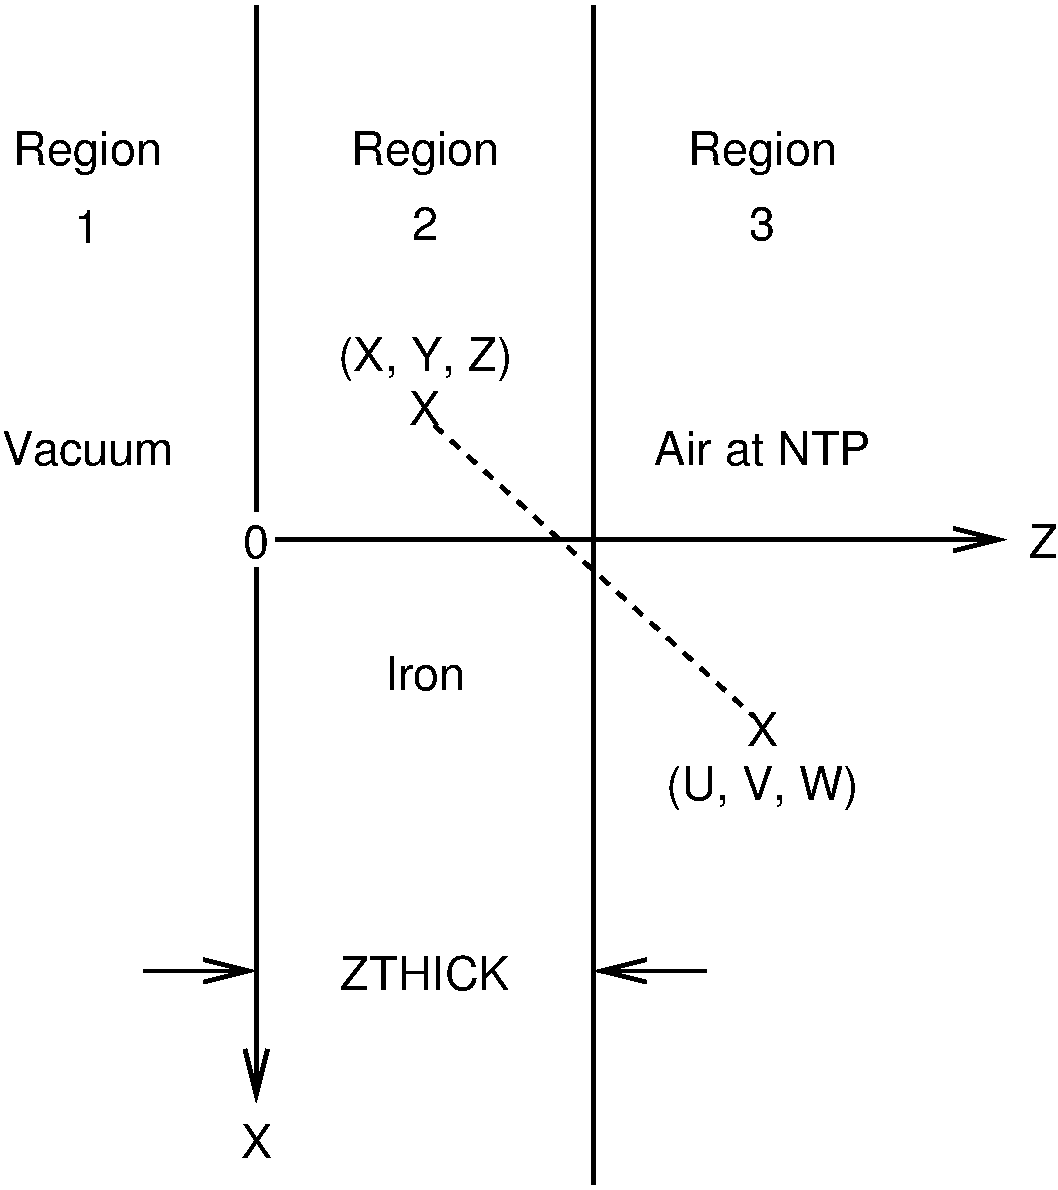
\includegraphics[width=10cm]{figures/3_region_ex}
   \end{center}
   \caption{A 3 region geometry example for HOWFAR.  The Y axis is into the
paper.}
   \label{fig_3_region_ex}
\end{figure}
Consider, as an example of how to write a {\tt HOWFAR} subroutine, the three
region geometry in fig~\ref{fig_3_region_ex}.  A particle is shown in
Region 2 with coordinates (X,Y,Z) and direction cosines (U,V,W).  We will
assume that the slab of thickness {\tt ZTHICK} is semi-infinite (x and
y-directions), and that particles are immediately discarded whenever they
go into Region 1 or Region 3.  The following {\tt HOWFAR} code is then
applicable:
\begin{verbatim}
     SUBROUTINE HOWFAR;
     COMIN/EPCONT,STACK/;      "common blocks needed in calculations"
     COMMON/GEOM/ZTHICK;       "slab thickness defined in main"
     IF(IR(NP) ~= 2) [IDISC=1; RETURN;]
     IF(W(NP) =  0.0) [RETURN; "particle going parallel to planes"]
     "check forward plane first since shower heading that way"
     "                                       most of the time"
     IF(W(NP) > 0.0) [DELTAZ=(ZTHICK-Z(NP))/W(NP); IRNEXT=3;]
     "otherwise, particle must be heading in backwards direction"
     ELSE [DELTAZ=-Z(NP)/W(NP); IRNEXT=1;]
     "now check with USTEP and reset things if necessary"
     IF(DELTAZ <= USTEP) [USTEP=DELTAZ; IRNEW=IRNEXT;]
     RETURN;  END;
\end{verbatim}
\index{HOWFAR!example}

\index{PLAN2P}
\index{\$PLAN2P}
A number of geometry subprograms and their macro equivalents are
distributed with the EGS Code System in order to make it easier to write
{\tt HOWFAR}.  For example, {\tt SUBROUTINE PLAN2P}, or its equivalent macro {\tt
\$PLAN2P}, could have been used in place of several lines above and the
program would have been easier to read.

\index{Bielajew, Alex}
For an advanced discussion of coding {\tt HOWFAR} routines, see Alex Bielajew's
PIRS-341 report ``HOWFAR and HOWNEAR: Geometry Modeling for Monte Carlo
Particle Transport''\cite{Bi95a}.


\subsection{Specifications for HOWNEAR}
\label{hownear}
\index{HOWNEAR!specifications}
\index{\$CALL-HOWNEAR}


As mentioned in section~\ref{hownear_macro}(page~\pageref{hownear_macro}),
for compatibility with previous  EGS4/PRESTA user codes,
EGSnrc formally requires a macro definition which defaults to:
\begin{verbatim}
REPLACE {$CALL-HOWNEAR(#);} WITH {CALL HOWNEAR({P1},X(NP),Y(NP),Z(NP),IRL);}
\end{verbatim}
where the variable {\tt \#} is {\tt tperp}, the closest distance to
any boundary.  If you are starting from scratch it is easiest to code
{\tt HOWNEAR} as a subroutine.
\index{EGS4}


{\tt SUBROUTINE HOWNEAR} is concerned with the geometry but its job is
somewhat simpler to define than for {\tt SUBROUTINE HOWFAR} since it need
only return one value, namely {\tt tperp}, the distance to the closest
boundary in {\bfseries any} direction.  Unlike {\tt HOWFAR}, {\tt HOWNEAR} passes the
transport parameters parameters to the subroutine as:
\begin{verbatim}
           SUBROUTINE HOWNEAR(tperp, x,y,z, irl);
\end{verbatim}
where \verb+x,y,z+ are the current positions of the particle and \verb+irl+
is its current region.  The rest of the information about the geometry is
passed in whatever {\tt COMMONs} contain the necessary information. In NRCC
user codes and the tutorial codes this is {\tt COMMON/GEOM/;} but it can be
called anything the user wants.

One simplification is that the routine does not have to handle regions
outside the geometry (as {\tt SUBROUTINE HOWFAR} must in order to have them
discarded).

In complex geometries, the mathematics of {\tt HOWNEAR} can become difficult and
sometimes almost impossible!  If it is easier for the user to compute
some lower bound to the nearest distance, this could be
used in {\tt HOWNEAR}.  In the worst case, one can return \verb+tperp+ as 0.0
in which case the code goes into single scattering mode if using the
exact boundary crossing algorithm.  In fact, this is an easy general way to
turn on single scattering throughout the entire geometry.

The following is an example of a {\tt HOWNEAR} routine for the geometry given
above in section~\ref{howfar} concerning {\tt HOWFAR}.
See also section~\ref{hownear_change} (page~\pageref{hownear_change}).
\begin{verbatim}
     SUBROUTINE HOWNEAR(tperp,X,Y.Z,IRL);
     COMMON/GEOM/ZTHICK; "slab thickness defined in main"
     tperp = min(Z,ZTHICK-Z);
     RETURN;  END;
\end{verbatim}
\index{HOWNEAR}



\subsection{Specifications for AUSGAB}
\label{ausgab}
\index{AUSGAB!specifications}

The subroutine {\tt AUSGAB} is called by EGS with the statement:
\begin{verbatim}
      CALL AUSGAB(IARG);
\end{verbatim}
The argument {\tt IARG} indicates the situation under which {\tt AUSGAB}
is being called.  {\tt IARG} can take on 35 values starting from zero
(i.e., {\tt IARG}=0 through {\tt IARG}=34), although only the first
five are called by default in EGSnrc.  The remaining 30 {\tt IARG}
values must be ``switched-on" by means of the array {\tt IAUSFL}.
The value for {\tt IARG} and the corresponding situations are given in
Table~\ref{tab_iausfl_low}.

On occasion one wants to terminate a particle histroy from withing AUSGAB.
To do this cleanly and efficiently set {\tt E(NP) = 0}. One can also set
the weight to zero if you do not want any {\tt EDEP} energy to be scored.

The {\tt IARG} values in table~\ref{tab_iausfl_low} are the ones
generally required in the majority of situations in which EGS is used
to simulate electromagnetic cascade shower development.  In particular,
{\tt IARG}=0 is useful whenever track lengths are being calculated or when
charged particle ionization loss is needed.  Also, as a check on energy
conservation, {\tt EDEP} can be summed in {\tt AUSGAB} for all {\tt IARG}
values less than 5.  The extended {\tt IARG} range allows the user to
extract additional information without making changes to the EGS coding.
To do this we have created the integer flag array, {\tt IAUSFL(J)},
for J=1 through 35.  It takes on values of 1 or 0 depending on whether
{\tt AUSGAB} is called or not, respectively.  For J=1 through 5, which
corresponds to {\tt IARG}=0 through 4, {\tt IAUSFL(J)=1} (default).
In other words, {\tt AUSGAB} is always called for the situations
listed in Table~\ref{tab_iausfl_low}.  For the remaining values of J,
corresponding to {\tt IARG}=5 through 34, {\tt IAUSFL(J)=0} (default).
The value for {\tt IARG} and the corresponding situations for this upper
set of {\tt IARG} values are shown in Table~\ref{tab_iausflg_other}.
\index{IAUSFL}
\index{IARG}
\index{PCUT}
\index{ECUT}
    \begin{table}[hbt]
\index{IAUSFL}
\index{IARG}
\index{PCUT}
\index{ECUT}
    \begin{center}
\caption{Values of {\tt IARG} which are on by default and for which energy is
deposited.}
    \label{tab_iausfl_low}
\vspace*{4mm}
    \begin{tabular}{ c   p{135mm}l  |}
    \hline
    {\tt IARG} & ~~~~~~~~~~~~~~~~~~~~~~~~~~~~~~~~Situation \\
    \hline
0	& Particle is going to be transported by distance TVSTEP.\\
    &\\
1	&Particle is going to be discarded because its energy is below the
cutoff {\tt ECUT} (for charged particles) or {\tt PCUT} (for photons)---but its energy
is larger than the corresponding PEGS cutoff AE or AP, respectively.\\
    &\\
2	& Particle is going to be discarded because its energy is below
both {\tt ECUT} and {\tt AE} (or {\tt PCUT} and {\tt AP}).\\
	&\\
3	& Particle is going to be discarded because the user requested it
(in {\tt HOWFAR} usually or by range rejection).  \\
	&\\
4	&The difference between the energy of the incident particle and
         all of the final products is being deposited locally. This
         energy is  due to sub-threshold relaxation events.\\
	&\\
\hline
\end{tabular}
\end{center}
\end{table}
\index{IARG} \index{IAUSFL}
\index{AUSGAB} \index{interogating EGSnrc}
    \begin{table}[htbp]
\index{Coster-Kronig electrons}
\index{IARG} \index{IAUSFL}
    \begin{center}
    \caption{Values of {\tt IARG} which are off by default.}
    \label{tab_iausflg_other}
     \vspace*{2mm}
    \begin{tabular}{ c c   p{125mm}l }
    \hline
    {\tt IARG} & {\tt IAUSFL} & ~~~~~~~~~~~~~~~~~~~~~~~~~~~~~~~~Situation \\
    \hline
5&6&  Particle has been transported by distance TVSTEP.\\
&&\\
6&7& A bremsstrahlung interaction is to occur and a call
             to BREMS is about to be made in ELECTR.\\
7&8& Returned to ELECTR after a call to BREMS was made.\\
&&\\
8&9& A Moller interaction is to occur and a call to
             MOLLER is about to be made in ELECTR.\\
9&10& Returned to ELECTR after a call to MOLLER was made.\\
&&\\
10&11&  A Bhabha interaction is to occur and a call to
             BHABHA is about to be made in ELECTR.\\
11&12& Returned to ELECTR after a call to BHABHA was made.\\
&&\\
12&13& An in-flight annihilation of the positron is to
             occur and a call to ANNIH is about to be made
             in ELECTR.\\
13&14& Returned to ELECTR after a call to ANNIH was made.\\
14&15&  A positron has annihilated at rest.\\
&&\\
15&16& A pair production interaction is to occur and a
             call to PAIR is about to be made in PHOTON.\\
16&17& Returned to PHOTON after a call to PAIR was made.\\
&&\\
17&18& A Compton interaction is to occur and a call to
             COMPT is about to be made in PHOTON.\\
18&19& Returned to PHOTON after a call to COMPT was made.\\
&&\\
19&20& A photoelectric interaction is to occur and a call
             to PHOTO is about to be made in PHOTON.\\
20&21& Returned to PHOTON after a call to PHOTO was made
             (assuming {\tt NP} is non-zero).\\
&&\\
21&22& Subroutine UPHI was just entered. Not entered in
all cases now since the sampling is done more efficiently directly in some
subroutines.\\
22&23& Subroutine UPHI was just exited.\\
&&\\
23&24& A coherent (Rayleigh) interaction is about to occur.\\
24&25& A coherent (Rayleigh) interaction has just occurred.\\
&&\\
25 &26& A fluorescent photon has just been created in RELAX.\\
26 & 27& A Coster-Kronig electron has just been created in RELAX.\\
27 &28& An Auger electron has just been created in RELAX.\\
&&\\
28 &29& A positron is about to annihilate at rest.\\
\hline
\end{tabular}
\end{center}
\end{table}

% Split the table onto the next page
\begin{table}[htbp]
    \begin{center}
    \caption{Values of {\tt IARG} which are off by default (continued).}
     \vspace*{2mm}
    \begin{tabular}{ c c   p{125mm}l }
    \hline
    {\tt IARG} & {\tt IAUSFL} & ~~~~~~~~~~~~~~~~~~~~~~~~~~~~~~~~Situation \\
    \hline
29 &30& A photonuclear event is about to occur and a call
            to PHOTONUC is about to be made in PHOTON.\\
30 &31& Returned to PHOTON after a call to PHOTONUC was made.\\
&&\\
31 &32& Electron impact ionization is about to occur and a call
            to eii\_sample is about to be made in MOLLER.\\
32 &33& Returned to MOLLER after a call to eii\_sample was made.\\
&&\\
33 &34& A fluorescent photon from relaxations was just discarded below
            PCUT and the energy stored in edep\_local.\\
34 &35& An electron from relaxations was just discarded below
            ECUT and the energy stored in edep\_local.\\
\hline
\end{tabular}
\end{center}
\end{table}

As an example of how to write an {\tt AUSGAB} subprogram, consider the previous
three region geometry (Fig. \ref{fig_3_region_ex}).  Suppose that we wish to
score (i.e., output on the line printer) only photons that go from Region 2
into Region 3.  The {\tt AUSGAB} subprogram that will accomplish this is given
below.  In this example we print out the stack variables plus {\tt IARG}.
\index{AUSGAB!example}
\begin{verbatim}
    SUBROUTINE AUSGAB(IARG);
    COMIN/STACK/;
    "only output information for photons that are discarded"
    "(by the user) in region 3"
    IF(IARG = 3 & IQ(NP) = 0 & IR(NP) =  3) [
        OUTPUT E(NP),X(NP),Y(NP),Z(NP),U(NP),V(NP),W(NP),
          IQ(NP),IR(NP),IARG;  (7G15.7,3I5);]
    RETURN;  END;
\end{verbatim}
The tutorial programs described in
section~\ref{tutorials}(page~\pageref{tutorials}) give examples of various
types of {\tt AUSGAB} routines.

\subsubsection{Checking for STACK overflow}
\index{EGS4} \index{\$MXSTACK}
\index{STACK overflow}
Unlike  EGS4, EGSnrc prevents the user from placing
too many particles on the {\tt STACK}. This is implemented via a macro
called {\tt \$CHECK-STACK(\#,\#);} which will terminate the execution if the
stack pointer exceeds {\tt \$MXSTACK}. This check takes some time (not much)
but to optimize the speed of a calculation, one might want to redefine it
as a null macro once one is moving to production runs.
\begin{verbatim}
      REPLACE {$CHECK-STACK(#,#);} WITH {;}
\end{verbatim}
Even if the above macro is nulled out, EGSnrc continues to verify that
there is adequate space on the stack whenever radiative splitting is being
used.
\index{\$CHECK-STACK}

\subsubsection{Status of the STACK at various AUSGAB calls}
\label{stack_status}
\index{STACK!order}
\index{EGS4}
In EGS4, the general rule was that after an interaction, the lowest energy
particle was always on the top of the {\tt STACK}. This general rule has
been relaxed in EGSnrc, partially because of the new physics, and partially
because memory is not as expensive as it once was.

\index{bound Compton scattering}
With the addition of relaxation events in EGSnrc, the possibilities
about what is on the stack after various events has become more complex
than in EGS4. For example, after a Compton scattering event in {\tt
EGS4}
({\tt IARG}=18), one could count on the {\tt STACK} having one more particle on it
compared to just before the call ({\tt IARG}=17). In EGSnrc, when bound compton
is being simulated, this is no longer the case.  Firstly, because of the
rejection techniques used to determine if the event actually took place
(see section~\ref{compton},page~\pageref{compton}) it is possible that only the
original photon is on the stack. At the opposite extreme, the scattered
photon and electron may be on the {\tt STACK} along with 2 or 3 relaxation
particles (fluorescent x-rays, Auger electrons, Coster-Kronig electrons).
Another complication occurs if Russian Roulette is being used since in this
case there can be events in which there is nothing left on the {\tt STACK} after
the event (e.g. after a pair event where the particles are discarded).
To help sort out these situations, EGSnrc has the variable {\tt
NPold} in {\tt COMIN STACK} which points to the position on the stack of the initiating particle
(the photon prior to Compton scattering, Rayleigh scattering, pair
production, photo-electric event or the electron prior to Moller scattering
or a bremsstrahlung event, etc).

Another change with EGSnrc is that the ordering of the resultant particles
is not rigorously set as lowest to highest energy.  This saves computing
time and with the reduced cost of memory, the issue of the size of the
{\tt STACK} is not so critical, at least not for low energy simulations ($<$100
MeV).  However, for high-energy simulations this may cause problems. To
overcome these the user code could define the macros {\tt
\$PARTICLE-SELECTION-MOLLER;} (where {\tt MOLLER} can be any interaction)
to sort the stack by energy after whatever interactions needed it. These
macros are by default null macros, but they are placed immediately after
the call to each subroutine which samples a type of event.
\index{\$PARTICLE-SELECTION-}

The ordering on the {\tt STACK} is summarized in the following.  Note that
the introduction of electron impact ionization and relaxation after other
than the photoelectric events has led to significant changes.
\begin{description}

\index{photoelectric interactions}
\item[Photoelectric] {\tt NPold} points at the photoelectron unless the initial
photon energy is $<$1~keV in which case there is an error message and an
electron with the photon's energy is created. Another exception occurs if
the photon's energy is less than the N-shell binding (which can only occur
for Z$\ge$96), in which case {\tt EDEP} is set to the photon's energy and a
photon of energy 0.0 is left at {\tt NPold}.  For normal events, the
particles from \verb^NPold+1^ to {\tt NP} are due to relaxation events.  If
internal Russian Roulette is being played (see section~\ref{rusrou}), it is
possible for {\tt NP} to be {\tt NPOLD - 1} after the event where there is
no fluorescent photon and all the resulting electrons are killed by the
Russian Roulette.  \index{Russian Roulette}

\index{bound Compton scattering}
\index{Compton scattering}
\item[Compton scattering] For Klein-Nishina modelling, the scattered photon and
electron are in {\tt NPold} and \verb^NPold+1 = NP^ respectively (i.e. the energy is not
ordered).  When bound compton scattering is
being modelled, there are several possibilities. At one extreme, since a
rejection technique is used, the scattering may not occur. In this case,
\verb^NPold = NP^.  If the scattering occurs, then the scattered photon and
compton electron are in \verb^NPold^ and \verb^NPold+1^, as in the Klein-Nishina case. If
there are any relaxation particles (i.e. \verb^NP > NPold+1^), they are found
in \verb^NPold+2^ to \verb^NP^.  There is a slight complication if the internal Russian
Roulette is being used (see section~\ref{rusrou})
since, if all the electrons disappear because of Russian Roulette, then
NPold=NP. To distinguish these two cases, the flag {\tt i\_survived\_RR}
can be used. It has a value 0 for the case of an unbound interaction being
rejected and has a value $>$ 0 if the interaction occurred and all
secondaries were eliminated by Russian Roulette.
\index{i\_survived\_RR}

\index{pair production}
\item[Pair Production] For pair production the electron and positron are
in {\tt NPold} and\\ \verb^NPold+1 = NP^ with the lower energy particle on the
top of the {\tt STACK} (at \verb^NP^). If internal Russian Roulette kills
the electron - positron pair, then,
\verb^NP = NPold-1^ unless this would leave \verb^NP = 0^, in which a
zero energy photon is placed on the {\tt STACK} with \verb^NP = 1^.

\index{Rayleigh scattering}
\item[Rayleigh scattering] In this case, the photon is still at
\verb^NPold^.

\index{bremsstrahlung!production}
\index{bremsstrahlung!splitting}
\item[Brem production] In this case, the resulting electron is
always at \verb^NPold^ and the photon is on top of the {\tt STACK} at \verb^NPold+1^, i.e. the
lowest energy particle is not necessarily on the top of the STACK. When
bremsstrahlung splitting is being used. The photons are between
\verb^NPold+1^ and
\verb^NP^. Note that they are not ordered by energy.

\index{Moller scattering}
\item[Moller scatter] There are 3 possible situations after a call to the
Moller routine. If a `standard' Moller scattering has occurred, the
resulting, lower energy electron is in \verb^NPold+1 = NP^ and the primary
is at \verb^NPold^. It is possible
that the incident electron's energy is below the threshold for creating a
secondary and the return is with \verb^NP^=\verb^NPold^. If this call to
Moller led to an electron impact ionization, the primary electron will be
at \verb^NPold^ and there may be relaxation events
from  \verb^NPold+1^ to \verb^NP^ although in the extreme case of all energy
deposition below threshold \verb^NP^=\verb^NPold^ and there is only the
primary electron.

\index{Bhabha scattering}
\item[Bhabha scatter] The resulting positron and electron are at
\verb^NPold^ and
\verb^NPold+1^, ordered by their energies.

\index{annihilation}
\item[Annihilation] The two resulting photons are at \verb^NPold^ and
\verb^NPold+1^
unless bremsstrahlung splitting is being used in which case the photons go
from \verb^NPold^ to \verb^N^P. The particle energies are not ordered.

\index{relaxation}
\item[Relaxation] There can be separate calls to AUSGAB after the
individual relaxation events (fluorescent photon, Coster-Kronig or Auger
electrons) but note that after the complete relaxation there may also be
ASUGAB calls post Moller, photoelectric and Compton and one should avoid
double counting.

\end{description}

\subsection{Terminating particle histories}
\label{termination}
\index{terminating particle history}
\index{weight}
\index{IDISC}
\index{WT=0.0}
The standard method to terminate a history is by setting
IDISC to a non-zero value in HOWFAR (see section~\ref{howfar},
page~\pageref{howfar}).  Another method is to set the weight of
a particle to 0.0, usually in AUSGAB under some conditions (e.g. when
doing Russian Roulette).  This technique is used in EGS4 by checking the
weight of a particle as it enters HOWFAR and setting IDISC non-zero if the
weight is zero.  This is somewhat wasteful since it means that various
parameters are calculated for this particle, despite the fact that it
is going to be discarded. In particular, we found that if we were also
using the standard photon forcing macro we got into an infinite loop.
This could have been corrected by re-coding the macro to handle weight
0.0 particles differently, but it was decided that we could save more
time by adding a test at the start of the new electron or new photon loops
whereby a particle is discarded immediately via the {\tt
USER-PHOTON-DISCARD} or {\tt USER-ELECTRON-DISCARD} if the weight is 0.0.
This generates a call to AUSGAB with {\tt IARG = 3}. Positrons discarded
this way do not create annihilation photons. Note that {\tt
ELKE} is not available with this call since it is assumed the particle
is being thrown away.  One should still have HOWFAR set {\tt IDISC = 1}
when the weight is 0.0, especially if the weight is set to zero for a
particle which is not new.


\subsection{Random number generators}
\label{rngs}
\index{random number generators}
\index{RANLUX}
\index{RANMAR}
\index{luxury level}

\index{EGS4}
EGSnrc is supplied with two random number generators, RANLUX
and RANMAR.  RANMAR is the generator used with EGS4 in the unix
distributions\cite{MZ91,Ma90a} and although it is known to fail certain
theoretical tests, we have no experience of it causing problems.
The RANLUX generator\cite{La94,Ja94}, which is treated as the default
generator with EGSnrc, is a similar sort of generator which comes
with a variety of ``luxury levels'', from 0 to 4 and a period of
greater than 10$^{165}$.  According to James, RANMAR has a
quality somewhere between luxury level 1 and 2 of RANLUX
and we have found
that it gives incorrect answers in some practical EGSnrc calculations
with luxury level 0. However, with luxury level 1 or higher we have
seen no problems.  We have utilized RANLUX as the default rng because
it allows explicit testing with higher quality sequences if there are
ever any doubts.

Both random number generators offer several important features. Firstly,
they are completely portable, producing the same sequences on different
machines, although RANMAR occasionally gets slightly out of sequence and
sometimes optimizers on a given machine will cause the sequences to differ.
We have not seen this behaviour with RANLUX.  An even more important
feature is that either generator can be initialized and guaranteed to
produce a random number sequence which is independent from other sequences.
This is very useful for doing runs in parallel on multiple machines.
\index{parallel processing}


The default generator is defined in {\tt
\$HEN\_HOUSE/specs/all\_common.spec} by the statement {\tt RANDOM =
\$(EGS\_SOURCEDIR)ranlux}. This can be changed to {\tt ranmar} or,
for individual user codes, it can be changed by adding the statement
{\tt RANDOM = \$(EGS\_SOURCEDIR)ranmar} to the {\tt user\_code.make}
file, somewhere before the {\tt SOURCES =} statement (if it exists).
See Report PIRS-877 for further information about {\tt make} files in
the EGSnrcMP environment\cite{Ka03}.

These files provide the following macros which the user is free to use in
their user code:
\begin{verbatim}
        ;COMIN/RANDOM/;
        $RANDOMSET#;
        $DEFAULT-LL   (1 by default)
        $RNG-INITIALISATION;    (which is only needed optionally)
        $INITIALIZE RNG USING # AND #; (a more useful version of the above)
        $STORE RNG STATE ON UNIT #;
        $PUT RNG STATE ON UNIT #;
        $RETRIEVE RNG STATE FROM UNIT #;
        $SHOW-RNG-STATE(#);
        $PRINT-RNG-STATE(#,#);
        $RNG-INPUTS(#,#,#,#);  (uses GET_INPUTS routine)
\end{verbatim}
\index{\$DEFAULT-LL}
To generate a random number, say {\tt RNUMBER}, include:
\begin{verbatim}
          $RANDOMSET RNUMBER;
\end{verbatim}
Wherever the user needs to use {\tt \$RANDOMSET\#;}, they must ensure
{\tt COMIN/RANDOM/} is present.
\index{RANDOM}
\index{macro!\$RANDOMSET}
\index{\$RANDOMSET}
If the user is happy with luxury level 1 and the same sequence for each
calculation, the RANLUX generator is self-initializing. However, to use
other luxury levels or other sequences, the user code should include
a statement of the type:
\begin{verbatim}
         $INITIALIZE RNG USING luxury_level AND iseed;
\end{verbatim}
where {\tt luxury\_level} is an integer between 0 and 4 and {\tt iseed}
is any positive integer (and if left 0, a default of {\tt 314159265} is used).
\index{\$INITIALIZE RNG USING}

For a standard production run of one of the NRC user codes (CAVRZnrc for
$^{60}$Co photons incident on a thimble chamber with splitting of 130) we
get the timing results shown in table~\ref{tab_ll_times}, although these
values are revised from the pre-2003 printings and depend on the details of
any simulation.  Given the iproblems encountered using luxury level 0,
luxury level 1 has been
adopted as the default with EGSnrc. However, given a new coding of RANMAR
to generate groups of random numbers using a function call, we find that
RANMAR is faster (by 5\% say overall).  The penalty ifor using higher
RANLUX luxury levels becomes increasingly more
important at higher luxury levels and a user may want to verify that for
their simulations, use of the higher level makes no difference. We would
appreciate being informed of any cases found where luxury level 1 was not
adequate.
\index{random number generators!timing}
\index{luxury level!timing}
\begin{table}[htb]
\begin{center}
\caption{Calculation times for runs with CAVRZnrc for the same calculations
along with estimates of the time taken by the random number generator at
different luxury levels.  The results for luxury level 0 are different when
high precision is obtained.\vspace{3mm}
\label{tab_ll_times}
}
\begin{tabular}{ |c c c c |}
\hline
Luxury level & total CPU time  & \multicolumn{2}{c|}{time taken by RANLUX} \\
             &  s &  s  & \%\\
\hline
&&&\\
0	&194	& 24 & 12\% \\
1	&210	& 39 & 18\% \\
2	&240	& 68 & 28\% \\
3	&315	& 142  &45\% \\
4	&415	& 242  &58\% \\
&&&\\
\hline
    \end{tabular}
    \end{center}
    \end{table}


When using the RANMAR generator, the initialisation looks like:
\begin{verbatim}
         $INITIALIZE RNG USING IXX AND JXX;
\end{verbatim}
where {\tt IXX} and {\tt JXX} are two integers seeds with:
\cen{{\tt  0$<$ IXX$<=$31328} and {\tt 0$<$JXX$<=$30081}}

The other macros are for use when saving the state of a random number
generator to disk and possibly restarting a run or other book keeping tasks.

There are two files available for use in codes doing correlated
sampling.  These files are:
\begin{verbatim}
       ranlux.correlations    or      ranmar.corrrelations
\end{verbatim}
These files define the macros:
\begin{verbatim}
        $STORE-RNG(#);
        $RESET-RNG(#);
\end{verbatim}
which store and reset an arbitrary number of random number states ($\le${\tt
\$MXRNGDIM} which is 5 by default).

Note: because of how the RANLUX generator is implemented, it is essential
that any redefined {\tt COMIN/RANDOM} must include an integer variable
called {\tt rng\_seed}. This variable is initialized to 999999 in {\tt
egs\_set\_default} which replaces {\tt BLOCK DATA} in the EGSnrcMP
environment\cite{Ka03}.
\index{RANDOM} \index{COMMON!RANDOM}
\index{random number generators}
\index{RANLUX}
\index{RANMAR}
\index{\$STORE-RNG}
\index{\$RESET-RNG}

\subsection{Summary of transport parameter}
\label{param_options}
\index{transport parameter summary}
\index{cross section options}


In many cases transport parameters and cross section options will be
controlled via an input file that uses a {\tt option = value} format
(\eg~all RZ user codes, all C++ codes). The following provides a summary
of the options available along with possible settings.

%%%%%%%%%%%%%%%%%%%%%%%%%%%%%%%%%%%%%%%%%%%%%%%%%%%%%%%%%%%%%%%%%%%%%%%%%%%%%%%
%
%  EGSnrc manual: transport parameters
%  Copyright (C) 2015 National Research Council Canada
%
%  This file is part of EGSnrc.
%
%  EGSnrc is free software: you can redistribute it and/or modify it under
%  the terms of the GNU Affero General Public License as published by the
%  Free Software Foundation, either version 3 of the License, or (at your
%  option) any later version.
%
%  EGSnrc is distributed in the hope that it will be useful, but WITHOUT ANY
%  WARRANTY; without even the implied warranty of MERCHANTABILITY or FITNESS
%  FOR A PARTICULAR PURPOSE.  See the GNU Affero General Public License for
%  more details.
%
%  You should have received a copy of the GNU Affero General Public License
%  along with EGSnrc. If not, see <http://www.gnu.org/licenses/>.
%
%%%%%%%%%%%%%%%%%%%%%%%%%%%%%%%%%%%%%%%%%%%%%%%%%%%%%%%%%%%%%%%%%%%%%%%%%%%%%%%
%
%  Author:          Frederic Tessier, 2011
%
%  Contributors:
%
%%%%%%%%%%%%%%%%%%%%%%%%%%%%%%%%%%%%%%%%%%%%%%%%%%%%%%%%%%%%%%%%%%%%%%%%%%%%%%%


\index{ECUT}
\begin{verbatim}
       Global ECUT=     Global (in all regions) electron transport cut
                        off energy (in MeV). If this input is missing,
                        AE(medium) will be used.
                        [ ECUT ]
\end{verbatim}
\index{PCUT}
\begin{verbatim}
       Global PCUT=     Global (in all regions) photon transport cut
                        off energy (in MeV). If this input is missing,
                        AP(medium) will be used.
                        [ PCUT ]
\end{verbatim}
\index{SMAX}
\begin{verbatim}
       Global SMAX=     Global (in all regions) maximum step-size
                        restriction for electron transport (in cm).
                        If missing, no geometrical step-size restrictions
                        will be employed. Note that if you use the default
                        EGSnrc electron-step algorithm, no SMAX-restriction
                        is necessary. Option is useful for transport in low
                        density materials (air) when PRESTA behaviour is
                        turned on (see below)
                        [ SMAXIR ]
\end{verbatim}
\index{ESTEPE}
\begin{verbatim}
       ESTEPE=          Maximum fractional energy loss per step.
                        Note that this is a global option only, no
                        region-by-region setting is possible. If missing,
                        the default is 0.25 (25%).
                        [ ESTEPE ]
\end{verbatim}
\index{XImax}
\begin{verbatim}
       XImax=           Maximum first elastic scattering moment per step.
                        Default is 0.5, NEVER use value greater than 1 as
                        this is beyond the range of MS data available.
                        [ XIMAX ]
\end{verbatim}
\index{boundary crossing algorithm}
\index{bca\_algorithm}
\index{exact\_bca}
\index{transport\_algorithm}
\begin{verbatim}
       Boundary crossing algorithm= EXACT (default), PRESTA-I
                        There are two selections possible: EXACT means
                        the algorithm will cross boundaries in a single
                        scattering (SS) mode, the distance from a boundary
                        at which the transition to SS mode is made is
                        determined by 'Skin depth for BCA' (see below).
                        The second option is PRESTA-I, if selected boundaries
                        will be crossed a la PRESTA, i.e. with lateral
                        correlations turned off and MS forced at boundaries.
                        Default is EXACT.
                        [ bca_algorithm, exact_bca ]
\end{verbatim}
\index{skin depth for BCA}\index{exact\_bca}
\index{skindepth\_for\_bca}
\begin{verbatim}
       Skin depth for BCA=
                        Determines the distance from a boundary (in elastic
                        MFP) at which the algorithm will go into single
                        scattering mode (if EXACT boundary crossing) or
                        switch off lateral correlations (if PRESTA-I boundary
                        crossing). Default value is 3 for EXACT or
                        exp(BLCMIN)/BLCMIN for PRESTA-I (see the PRESTA paper
                        for a definition of BLCMIN). Note that if you choose
                        EXACT boundary crossing and set Skin depth for BCA
                        to a very large number (e.g. 1e10), the entire
                        calculation will be in single-scattering mode. If you
                        choose PRESTA-I boundary crossing and make Skin depth
                        for BCA large, you will get default EGS4 behaviour
                        (no PRESTA).
                        [ skindepth_for_bca ]
\end{verbatim}
\index{electron step algorithm}
\begin{verbatim}
       Electron-step algorithm= PRESTA-II (default), PRESTA-I (legacy)
                        Determines the algorithm used to take into account
                        lateral and longitudinal correlations in a
                        condensed history step.
                        [ transport_algorithm ]
\end{verbatim}
\index{spin effects}
\index{spin\_effects}
\begin{verbatim}
       Spin effects=    Off, On (default)
                        Turns off/on spin effects for electron elastic
                        scattering. Spin On is ABSOLUTELY necessary for
                        good backscattering calculations. Will make a
                        difference even in `well conditioned' situations
                        (e.g. depth dose curves for RTP energy range
                        electrons).
                        [ spin_effects ]
\end{verbatim}
\index{brems angular sampling}
\index{IBRDST}
\begin{verbatim}
       Brems angular sampling= Simple, KM (default)
                        If Simple, use only the leading term of the Koch-Motz
                        distribution to determine the emission angle of
                        bremsstrahlung photons. If KM, complete
                        modified Koch-Motz 2BS is used (modifications
                        concern proper handling of kinematics at low energies,
                        makes 2BS almost the same as 2BN at low energies).
                        [ IBRDST ]
\end{verbatim}
\index{brems cross section}
\index{ibr\_nist}
\begin{verbatim}
       Brems cross sections= BH (default), NIST, NRC
                        If BH is selected, the Bethe-Heitler bremsstrahlung
                        cross sections (Coulomb corrected above 50 MeV)
                        will be used. If NIST is selected, the NIST brems
                        cross section data base (which is the basis for
                        the ICRU radiative stopping powers) will be employed.
                        Differences are negligible for E > ,say, 10 MeV,
                        but significant in the keV energy range. If NRC is
                        selected, the NRC brems cross-section data base will
                        be used, which is a version of the NIST data base
                        with corrected electron-electron brems contributions
                        (corrections to the NIST data is typically only
                        significant for low values of the atomic number Z
                        and for k/T < 0.005).
                        [ ibr_nist ]
\end{verbatim}
\index{triplet production}
\index{itriplet}
\begin{verbatim}
       Triplet production= On or Off (default).  Turns on/off simulation
                        of triplet production.  If On, then Borsellino's
                        first Born approximation is used to sample triplet
                        events based on the triplet cross-section data.
                        [ itriplet ]
\end{verbatim}
\index{bound Compton scattering}
\index{IBCMP}
\begin{verbatim}
       Bound Compton scattering=  On, Off, Simple or norej (default)
                        If Off, Compton scattering will be treated with
                        Klein-Nishina, with On Compton scattering is
                        treated in the Impulse approximation.
                        With Simple, the impulse approximation incoherent
                        scattering function will be used (i.e., no Doppler
                        broadenning). With norej the actual total bound
                        Compton cross section is used and there are no
                        rejections at run time.
                        Make sure to turn on for low energy applications,
                        not necessary above, say, 1 MeV.
                        [ IBCMP ]
\end{verbatim}
\index{radiative Compton corrections}
\index{radc\_flag}
\begin{verbatim}
       Radiative Compton corrections= On or Off (default). If On, then
                        include radiative corrections for Compton scattering.
                        Equations are based on original Brown & Feynman
                        equations (Phys. Rev. 85, p 231--1952).  Requires
                        a change to the user codes Makefile to include
                        $(EGS_SOURCEDIR)rad_compton1.mortran in the
                        SOURCES (just before
                        $(EGS_SOURCEDIR)get_inputs.mortran).
                        [ radc_flag ]
\end{verbatim}
\index{electron impact ionization}
\index{eii\_flag}
\begin{verbatim}
       Electron Impact Ionization= Off (default), On, casnati, kolbenstvedt,
                        gryzinski or penelope.  If set to On or ik, then
                        use Kawrakow's theory to derive EII cross-sections.
                        If set to casnati, then use the cross-sections of
                        Casnati (from file $HEN_HOUSE/data/eii_casnati.data).
                        Similar for kolbenstvedt, gryzinski and penelope.
                        This is only of interest in kV X-ray calculations.
                        Note that the user can supply their own EII
                        cross-section data as well. The requirement is that
                        the file eii_suffix.data exists in the $HEN_HOUSE/data
                        directory, where suffix is the name specified.
                        Entry is case-sensitive except for Off, On or ik.
                        [ eii_flag, eii_xfile ]
\end{verbatim}
\index{pair angular sampling}
\index{IPRDST}
\begin{verbatim}
       Pair angular sampling= Off, Simple (default), KM.
                        If off, pairs are set in motion at an angle m/E
                        relative to the photon direction (m is electron rest
                        energy, E the photon energy). Simple turns on
                        the leading term of the angular distribution
                        (this is sufficient for most applications),
                        KM (comes from Koch and Motz) turns on using 2BS
                        from the article by Koch and Motz.
                        Default is Simple, make sure you always use
                        Simple or KM
                        [ IPRDST ]
\end{verbatim}
\index{pair cross sections}
\index{pair\_nrc}
\begin{verbatim}
       Pair cross sections= BH (default) or NRC.  If set to BH, then use
                        Bethe-Heitler pair production cross-sections.  If set
                        to NRC, then use NRC pair production cross-sections
                        (in file $HEN_HOUSE/data/pair_nrc1.data).  Only
                        of interest at low energies, where the NRC cross-
                        sections take into account the asymmetry in the
                        positron-electron energy distribution.
                        [ pair_nrc ]
\end{verbatim}
\index{photon cross sections}
\index{photon\_xsections}
\begin{verbatim}
       Photon cross sections= Photon cross-section data.  Current options are
                        si (Storm-Israel--the default), epdl (Evaluated Photon
                        Data Library), and xcom.  Allows the user to use photon
                        cross-sections other than the default PEGS4 (Storm-
                        Israel) values.  Note that the user can supply their
                        own cross-section data as well.  The requirement is
                        that the files
                        photon_xsections_photo.data,
                        photon_xsections_pair.data,
                        photon_xsections_triplet.data, and
                        photon_xsections_rayleigh.data exist in the
                        $HEN_HOUSE/data directory, where photon_xsections
                        is the name specified.
                        Entry is case-sensitive except for the pegs4 option.
                        [ photon_xsections ]
\end{verbatim}
\index{photon cross sections!output}
\index{xsec\_out}
\begin{verbatim}
       Photon cross-sections output= Off (default) or On.  If On, then
                        a file $EGS_HOME/user_code/inputfile.xsections is
                        output containing photon cross-section data used.
                        [ xsec_out ]
\end{verbatim}
\index{compton cross sections}
\index{comp\_xsections}
\begin{verbatim}
       Compton cross sections= Bound Compton cross-section data.  User-
                        supplied bound Compton cross-sections in the file
                        $HEN_HOUSE/data/comp_xsections_compton.data, where
                        comp_xsections is the name supplied for this input.
                        This is only used if Bound Compton scattering= Simple
                        and is not available on a region-by-region basis
                        (see below).  The default file (ie in the absence
                        of any user-supplied data) is compton_sigma.data.
                        [ comp_xsections ]
\end{verbatim}
\index{Rayleigh scattering}
\index{Rayleigh scattering!custom form factors}
\index{IRAYLR}
\begin{verbatim}
       Rayleigh scattering= Off, On (default), custom
                        If On, turns on coherent (Rayleigh) scattering.
                        Default is On. Should be turned on for low energy
                        applications. If custom, user must provide media names
                        and form factor files for each desired medium. The
                        rest of the media use the default atomic form factors.
                        Not set to On by default for historical reasons since
                        a PEGS4 data set is not required anymore.
                        [ IRAYLR ]
\end{verbatim}
\index{iray\_ff\_media}
\begin{verbatim}
       ff media names = A list of media names (must match media found in
                        PEGS4 data file) for which the user is going to
                        provide custom Rayleigh form factor data.
                        [ iray_ff_media($MXMED) ]
\end{verbatim}
\index{iray\_ff\_file}
\begin{verbatim}
       ff file names = A list of names of files containing the Rayleigh
                       form factor data for the media specified by
                       the ff media names = input above.  Full directory
                       paths must be given for all files, and for each medium
                       specified, iray_ff_media(i), there must be a
                       corresponding file name, iray_ff_file(i).  For
                       example files, see the directory
                       $HEN_HOUSE/data/molecular_form_factors.
                       [ iray_ff_file($MXMED) ]
\end{verbatim}
\index{photonuclear attenuation}
\index{IPHOTONUCR}
\begin{verbatim}
       Photonuclear attenuation= Off (default) or On
                        If On, models the photonuclear effect. Current
                        implementation is crude. Available on a
                        region-by-region basis (see below)
                        [ IPHOTONUCR ]
\end{verbatim}
\index{photonuclear cross sections}
\index{photonuc\_xsections}
\begin{verbatim}
       Photonuclear cross sections= Total photonuclear cross sections. User-
                        supplied total photonuclear cross-sections in
                        $HEN_HOUSE/data/photonuc_xsections_photonuc.data,
                        where photonuc_xsections is the name supplied for
                        this input (case sensitive). In the absence of
                        any user-supplied data, or if photonuc_xsections
                        is set to 'default', the default file is
                        iaea_photonuc.data.
                        [ photonuc_xsections ]
\end{verbatim}
\index{photoelectron angular sampling}
\index{IPHTER}
\begin{verbatim}
       Photoelectron angular sampling= Off or On (default)
                        If Off, photo-electrons get the direction of the
                        `mother' photon, with On, Sauter's formula is
                        used (which is, strictly speaking, valid only for
                        K-shell photo-absorption).
                        If the user has a better approach, replace the macro
                            $SELECT-PHOTOELECTRON-DIRECTION;
                        The only application encountered where this option
                        made a small difference was a big ion chamber
                        (cavity size comparable with electron range)
                        with high-Z walls in a low energy photon beam.
                        [ IPHTER ]
\end{verbatim}
\index{atomic relaxations}
\index{IEDGFL}
\begin{verbatim}
       Atomic relaxations= Off, On, eadl (default), simple
                        On defaults to eadl.
                        When simulating atomic relaxations:
                        - In photo-electric absorption events, the element
                          (if material is mixture) and the shell the photon
                          is interacting with are sampled from the appropriate
                          cross sections
                        - Shell vacancies created in photoelectric,
                          compton and electron impact ionization events
                          are relaxed via emission of fluorescent X-Rays,
                          Auger and Koster-Cronig electrons.
                          The eadl option features a more accurate treatment
                          of relaxation events and uses binding energies
                          consistent with those in of the photon cross sections
                          used in the simulation.  If using mcdf-xcom or
                          mcdf-epdl photon cross sections, you cannot use
                          the simple option and this will automatically get
                          reset to eadl. Make sure to use eadl or simple for
                          low energy applications.
                          [ IEDGFL ]
\end{verbatim}

\noindent
Atomic relaxations, Rayleigh scattering, Photoelectron angular sampling,
Bound Compton scattering and photonuclear effect
can also be turned On/Off on a region-by-region basis. An example for
Atomic relaxations on a region-by-region basis is:

\begin{verbatim}
       Atomic relaxations= On in Regions   or
       Atomic relaxations= Off in regions
\end{verbatim}

Then define the regions in which you want
the feature to be turned on:

\begin{verbatim}
       Bound Compton start region=
       Bound Compton stop region=
                or
       Rayleigh start region=
       Rayleigh stop region=
                or
       Relaxations start region=
       Relaxations stop region=
                or
       PE sampling start region=
       PE sampling stop region=
\end{verbatim}
each followed by a list of one or more
start and stop regions separated by commas.
Example:
\begin{verbatim}
        Atomic relaxations= On in Regions
        Relaxations start region=  1, 40
        Relaxations stop region=  10, 99
\end{verbatim}
will first turn off relaxations everywhere and
then turn on in regions 1-10 and 40-99.
Note that the input is checked against minimum
and maximum region numbers and ignored if
\verb+start region < 1+ or \verb+stop_region > $MXREG+ or
\verb+start region > stop region+.

\verb+ECUT+, \verb+PCUT+ and \verb+SMAX+ can also be set on a
region-by-region basis. To do so, include in the input file
\begin{verbatim}
         Set XXXX=              f_value1, f_value2, ...
         Set XXXX start region= i_value1, i_value2, ...
         Set XXXX stop region=  j_value1, j_value2, ...
\end{verbatim}
where \verb+XXXX+ is \verb+ECUT+, \verb+PCUT+ or \verb+SMAX+,
\verb+f_value1+, \verb+f_value2+,...
are the desired values for \verb+XXXX+ and \verb+i_value_i+ and
\verb+j_value_i+ are the start and stop regions.


\subsection{Variance Reduction Options}
\label{VRO}
\index{variance reduction}
Three forms of variance reduction techniques have been implemented directly
into the EGSnrc system in order to allow for more efficient calculations.
With EGS4 user codes they had to be implemented via calls to {\tt
AUSGAB} or
other means, and this led to inefficiencies.  In all three cases, if the
user does nothing to turn on these options explicitly, then they are NOT
used.
\index{EGS4}

\subsubsection{Range rejection}
\label{range_rejection}

\index{range rejection}
\index{variance reduction}
\index{variance reduction!range rejection}
\index{E\_RANGE}
Within EGSnrc the range of the electron is available at every step. This is
not the true range, but the range determined by:
\[ {\tt E\_RANGE} = \int_{E_{min}}^E \frac{dE^\prime}{L(E^\prime,AE)}\]
where $L(E^\prime,AE)$ is the restricted stopping power for a given value
of AE and $E_{min}$ is the lowest energy for which PEGS4 produces a
stopping power (this is somewhat less than AE, but not much).
The value of {\tt E\_RANGE} is an
upper limit on the distance an electron can travel in the simulation
because discrete events may shorten the pathlength.

\index{\$RANGE-DISCARD}
\index{macro!\$RANGE-DISCARD}
Range rejection is implemented by a macro {\tt \$RANGE-DISCARD} checks
the electron range against the distance to the nearest boundary on
every step. The history is terminated whenever the range is shorter than
the distance to the boundary and if requested by the user.  Since the
range and distance are calculated for other purposes, this check is
very fast and can save a large amount of time, especially in large
regions. Since this is a user controlled discard, it goes via the {\tt
USER-ELECTRON-DISCARD}, generating and {\tt {\tt IARG} = 3}   call to {\tt
AUSGAB}.
\index{USER-ELECTRON-DISCARD}   \index{AUSGAB}

This technique
does involve an approximation since the electron could emit a
brem photon which could escape the region, even if the electron
itself could not.  To control the extent of this approximation, the range
rejection is done only if the electron's energy is below an energy
threshold which can be set for every region, viz {\tt e\_max\_rr}. By
judicial choice of this value, the approximation can be made very accurate
while still obtaining very significant gains in efficiency (see
ref~\cite{Ro95} for a detailed discussion, where the parameter {\tt ESAVE}
in that paper is equivalent to {\tt e\_max\_rr} here).

Range rejection is implemented on a regional basis by setting the flags
{\tt i\_do\_rr(irl)} to 1 for all regions {\tt irl} for which range
rejection is required and by assigning values to the array {\tt
e\_max\_rr(irl)}. Note that if {\tt e\_max\_rr(irl)} is not assigned a value,
its default value of 0.0 effectively turns off range rejection, even
if {\tt i\_do\_rr(irl)} value is 1.  Both arrays are in {\tt
COMIN/EGS-VARIANCE-REDUCTION}. They need be set before the first
call to {\tt SHOWER}.  Note that {\tt e\_max\_rr(irl)} refers to the
electrons total energy (i.e. includes the rest mass, as does {\tt ECUT}).
\index{EGS-VARIANCE-REDUCTION} \index{e\_max\_rr}
\index{i\_do\_rr} \index{range rejection}

The user is also free to implement other, possibly more efficient forms of
range rejection. This is done by defining the macro {\tt
\$USER-RANGE-DISCARD} which is called immediately after the above macro
since in general, the macro {\tt \$RANGE-DISCARD} executes very quickly
and can avoid use of the user's, presumably more time consuming range
rejection.  An example of {\tt
\$USER-RANGE-DISCARD} is given in CAVRZnrc where range rejection is done on
any particle which cannot reach the region where the dose is required. This
can terminate many histories earlier than {\tt \$RANGE-DISCARD} because it
tests against getting to the region of interest as opposed to just getting
out of the local region.  However, it requires some approximations and
takes longer to compute on each step.
\index{\$USER-RANGE-DISCARD}
\index{range rejection}

\subsubsection{Bremsstrahlung Splitting}
\label{brem_splitting}
\index{bremsstrahlung!splitting}
\index{variance reduction!brem splitting}
\index{nbr\_split}
Bremsstrahlung splitting is a technique which can provide a factor of 4 or
more
improvement in efficiency when modelling brem beams generated
by medical accelerators\cite{Ro95}.  Each time an electron emits a photon,
the simulation emits an arbitrary number of brem photons with
their weight suitably reduced. The electron's energy is decremented by the
energy given off by one of these photons. This preserves accurate
energy loss straggling of the electron at the expense of no longer having
exact energy conservation for each history, although energy is conserved
``on average''.  The advantage of doing this splitting within the routine
BREMS is that various constants for the electron's energy are only
calculated once and the sampling is therefore faster.  The electron is
always found at \verb^NPold^ on the {\tt STACK} and the photons are not sorted by energy.

To accomplish bremsstrahlung  splitting, the variable {\tt nbr\_split} which
is in\\ {\tt COMIN/EGS-VARIANCE-REDUCTION} must be set to the number of
brem photons wanted at each discrete interaction. See
section~\ref{rad_split} (page~\pageref{rad_split}).

There are no internal limits on the number of splits that may be used
except that the stack size, {\tt \$MXSTACK}, may not be exceeded.  The user
code can override the value of {\tt \$MXSTACK} if a larger value is needed.

\index{Russian Roulette}
Note that once
set, EGSnrc will split brem at all generations.  This is
appropriate when Russian Roulette is being played since it means that
second generation bremsstrahlung photons will have the same weight as first
generation photons.  However, it can become very time consuming and counter
productive when Russian Roulette is not being played because second and
higher order bremsstrahlung photons have much smaller weights. To overcome
this problem, the user might want to use calls to {\tt AUSGAB} to reduce the
value of {\tt nbr\_split} after each first generation bremsstrahlung
interaction and then re-initialize it at the start of the next history.
This is the technique used in the BEAM code\cite{Ro95,Ro98a}.
\index{BEAM code}


\subsubsection{Russian Roulette}
\label{rusrou}
\index{variance reduction!Russian Roulette}
\index{Russian Roulette}
\index{i\_play\_RR}
\index{prob\_RR}
\index{nbr\_split}
\index{i\_survived\_RR}
\index{EGS4}
Russian Roulette is a standard variance reduction technique which in {\tt
EGS4}
had to be done via call to {\tt AUSGAB}. This works but is somewhat slower than
need be. For example, say that the particles created in a pair
event are to be discarded. In EGS4 the sampling routines must still
determine all their parameters and then remove them from the {\tt STACK} whereas
in EGSnrc Russian Roulette is played prior to the sampling, and then
not done if not needed. In less dramatic cases, the EGSnrc approach avoids
extra steps were the EGS4 system had to go through to eliminate the
particle.

Russian Roulette, as implemented in EGSnrc, is a user option which is turned on by
setting the integer flag {\tt i\_play\_RR} to 1 and by setting the
probability {\tt prob\_RR} to an appropriate value. Both these parameters
are in {\tt COMIN/EGS-VARIANCE-REDUCTION}.

If Russian Roulette is being used in conjunction with bremsstrahlung
splitting, the appropriate value of {\tt prob\_RR} is {\tt 1./nbr\_split}.

The integer variable {\tt i\_survived\_RR} is also in  {\tt
COMIN/EGS-VARIANCE-REDUCTION}. It is 0 if Russian Roulette is not played or
if all particles survived when Russian Roulette was played on the previous
interaction.  Otherwise, its value tells how many particles were discarded
by Russian Roulette on the previous interaction.
\index{Russian Roulette}



\subsection{Complete Users Codes Examples}
For several examples of complete EGSnrc user codes, see the TUTOR codes
discussed in section~\ref{tutorials}. The EGSnrc distribution also comes
with several NRC user codes which have examples of many features\cite{Ro00}
but they have grown up over the years and have been patched so often that
they are hard to follow.

\subsection{Some Utility codes}
\subsubsection{SUBROUTINE WATCH}
\index{WATCH}
\index{IWATCH}
\index{SUBROUTINE WATCH}
\index{EGS\_Windows}
{\tt SUBROUTINE WATCH} is in the file {\tt nrcaux.mortran}. With a few simple
statements in a user code, it can print a listing to the screen of what is
happening in each history.  This is very useful for debugging purposes. We
strongly recommend that it be used with all user codes.  It also creates
output suitable for the EGS\_Windows graphic display system\cite{TR99a}.
For more information, see {\tt tutor4.mortran} for an example of a simple
code with WATCH included (see section~\ref{tutor4}, page~\pageref{tutor4}).

\subsubsection{ranlux\_test.mortran and ranmar\_test.mortran}
\index{test!RANLUX}
\index{test!RANMAR}
\index{ranlux\_test.mortran}
\index{ranmar\_test.mortran}
\index{random number generators!portability}
These little codes can be used to verify that the ranlux and
ranmar random number generators are working correctly on your
system. Since these generators produce machine independent
random numbers, the values should be identical on all machines.
They are found on {\tt \$HEN\_HOUSE/user\_codes/ranlux\_test/} and  {\tt
\$HEN\_HOUSE/user\_codes/ranmar\_test/}. Each can be compiled and executed
as a user code.  The output is self explanatory but basically
they both calculate
1 million random numbers and compare their sums to the expected values.
See the comments at the top of the source code for further information.

Note that even with identical random number sequences, the results of a
full EGSnrc calculation may not be identical on different machines or at
different optimization levels.  This is because statements like
\begin{verbatim}
          IF ( A < C/D) ) GOTO n;
\end{verbatim}
may branch differently, depending on how many digits are stored in C/D on
different machines or at different levels of optimization.

\subsubsection{EXAMIN}
\index{EXAMIN}
\index{user codes!EXAMIN}
\label{examin}
\index{xmgr}
\index{HOW\_to\_get\_xmgr}
The user code EXAMIN is distributed with the system. It provides easy
access to the underlying data produced by PEGS4. EXAMIN tabulates many
cross sections and if you have installed the
{\tt xmgr} graphics package it also plots the data (see the file\\ {\tt
\$HEN\_HOUSE/utils/HOW\_to\_get\_xmgrace} for information about {\tt
xmgrace}).
The code outputs quantities such as the gamma mean free path, the relative
contributions from the various components of the photon cross sections, the
mean free path to discrete interactions for electrons, etc.  It is a useful
template for seeing how to access the data base.  Note that the data
presented are those from PEGS4. Although EGSnrc can model bound Compton
scattering, this is done using a rejection technique and this code does not
allow access to the bound Compton cross sections, only the Klein Nishina
cross sections.
%  If you are using the {\tt xmgrace} package instead of the
%  {\tt xmgr} package, {\tt xmgr} must be replaced by {\tt xmgrace}
%  in the source code for {\tt examin.mortran} in two obvious places.

% \subsubsection{show\_settings}
% \label{settings}
% \index{show\_settings}
% \index{settings}
% This is a simple script which will display all the variables and aliases
% which are set or defined for use with the EGSnrc system (mostly in {\tt
% Cshrc\_additions\_for\_egsnrc}).


% \subsubsection{test\_distribution}
% \label{test_distribution}
% \index{test\_distribution}
% \index{test!distribution}
%
% This script is found on {\tt \$HEN\_HOUSE/scripts} after installation
% and the command {\tt test\_distribution} is aliased to it in {\tt
% egsnrc\_cshrc\_additions} and {\tt egsnrc\_bashrc\_additions}.
% It is executed with no arguemnts, and to capture the output as:
% \begin{verbatim}
             % test_distribution >& test_distribution.output &
% \end{verbatim}
% This script compiles all the user and tutorial codes and runs them with
% short
% test input files.  You must read the output file carefully since it will
% continue even when some or all of the codes fail to compile or execute!
% Once you get this script to execute cleanly
% your system is definitely in good shape. The results
% for running this script on various systems are found on {\tt
% \$HEN\_HOUSE/test\_distribution\_outputs}.
% \index{test\_distribution\_outputs}

\subsection{Latest additions}
\subsubsection{Charged particle transport under electromagnetic fields}
\label{EMF_macros_implementation}
Bielajew's EGS4 macros for transport under electromagnetic (EM) fields were adapted for EGSnrc by Amir Keyvanloo and
others from the Cross Cancer Institute in Edmonton. These macros have been included in the current EGSnrc release.
To turn on transport under EM fields, users must add the file {\tt emf\_macros.mortran} to the {\tt MORTRAN} sources to be compiled. The subroutine {\tt ELECTR} in {\tt egsnrc.mortran} contains macro replacements which are empty by default, but which are activated when including the EM macros.

To include these macros in a MORTRAN user code, append {\tt emf\_macros.mortran} to {\tt SOURCES} variable in file
{\tt user\_code.make} (user\_code can be any MORTRAN user code other than a BEAMnrc user code):
\begin{verbatim}
 ...
SOURCES = \
        $(EGS_SOURCEDIR)egsnrc.macros \
        ...
        $(EGS_SOURCEDIR)emf_macros.mortran \
        $(USER_CODE).mortran \
        ...
        $(EGS_SOURCEDIR)get_inputs.mortran\
        $(EGS_SOURCEDIR)get_media_inputs.mortran\
        ...
        $(EGS_SOURCEDIR)pegs4_routines.mortran \
        $(EGS_SOURCEDIR)egsnrc.mortran
 ...
\end{verbatim}

To include these macros in an existing BEAMnrc user code, append {\tt emf\_macros.mortran} to {\tt SOURCES} variable in file
{\tt source.make}:
\begin{verbatim}
SOURCES = $(EGS_SOURCEDIR)egsnrc.macros \
          ...
          $(EGS_SOURCEDIR)emf_macros.mortran \
          ...
          $(BEAM_HOME)beamnrc_user_macros.mortran \
          ...
          $(BEAM_CODE)_macros.mortran \
          $(EGS_SOURCEDIR)egs_utilities.mortran \
          $(BEAM_HOME)beam_main.mortran\
          $(BEAM_HOME)beamnrc.mortran \
          ...
          $(EGS_SOURCEDIR)egsnrc.mortran

\end{verbatim}
In the case of a BEAMnrc source library, append {\tt emf\_macros.mortran} to {\tt LIB\_SOURCES} variable in file
{\tt source.make}:
\begin{verbatim}
LIB_SOURCES = $(BEAM_HOME)beam_lib.macros \
          $(EGS_SOURCEDIR)egsnrc.macros \
          ...
          $(EGS_SOURCEDIR)emf_macros.mortran \
          ...
          $(BEAM_HOME)beamnrc_user_macros.mortran \
          ...
          $(BEAM_CODE)_macros.mortran \
          $(BEAM_HOME)beam_lib.mortran\
          $(BEAM_HOME)beamnrc.mortran \
          ...
          $(EGS_SOURCEDIR)egsnrc.mortran
\end{verbatim}

For C++ user codes one must append {\tt emf\_macros.mortran} to the {\tt EGSPP\_USER\_MACROS} variable in
the {\tt Makefile}:
\begin{verbatim}
 ...
# Specify the name of the user code.
# The name of the executable is determined from this variable.
#
USER_CODE = cavity

# The following can be used to add user macros and mortran subroutines.
# The file(s) specified here are added after egsnrc.macros, machine.macros
# and egs_c_interface2.macros but before any files that have
# executable code.
#
#EGSPP_USER_MACROS = cavity.macros
EGSPP_USER_MACROS = cavity.macros  \
                    $(EGS_SOURCEDIR)emf_macros.mortran
 ...
\end{verbatim}

Details of the field and the step size restriction are entered by input in the MC transport parameters section:
\begin{itemize}
\item For magnetic fields:
\begin{verbatim}
:start MC transport parameter:
 ...
 Magnetic Field = 0, 1.5, 0 # magnetic field in T
 EM ESTEPE = 0.02
 ...
:stop MC transport parameter:
\end{verbatim}

\item For electric fields:
\begin{verbatim}
:start MC transport parameter:
 ...
 Electric Field = 0, 3, 0 # electric field in V/cm
 EM ESTEPE = 0.02
 ...
:stop MC transport parameter:
\end{verbatim}
\end{itemize}

Please note than one can define both, an electric and a magnetic field. The {\tt EM ESTEPE}
entry sets the value for the step size restrictions based on energy loss, field change and
direction change. For instance, in the static $\vec{B}_0$ field case of section \ref{EMF_macros_algorithm},
{\tt EM ESTEPE} corresponds to the $\delta$ value of Eq(\ref{uchange_restriction}). By default it is set to 0.02.

\subsubsection{EADL atomic relaxations}
In EGSnrc the relaxation cascade of inner shell vacancies is an independent process that is initiated each time
a vacancy is created
\begin{itemize}
  \item In photo-absorption, bound Compton scattering, and electron impact ionization processes.
  \item Future: triplet production, electron-electron bremsstrahlung
\end{itemize}

The default implementation include relaxation events from:
\begin{itemize}
\item All shells with binding energies above 1 keV
\item All radiative and non-radiative transitions to/from K-, LI-, LII and LIII-shells
\item All radiative and non-radiative transitions to/from ``average'' M and N-shells.
\end{itemize}

An option to remove above limitations by using EADL atomic relaxation data has been available in EGSnrc since 2011.
% User must set macro \$EADL\_RELAX to .true. in file egsnrc.macros.
The way to turn on EADL relaxation is by setting macro \$EADL\_RELAX to .true. in egsnrc.macros or in the user-code. It is currently set to .false. by default.

%following may be needed to get next section start on odd page
%\newpage
%\mbox{}


%%%%%%%%%%%%%%%%%%%%%%%%%%%%%%%%%%%%%%%%%%%%%%%%%%%%%%%%%%%%%%%%%%%%%%%%

%		Tutorial Programs

%%%%%%%%%%%%%%%%%%%%%%%%%%%%%%%%%%%%%%%%%%%%%%%%%%%%%%%%%%%%%%%%%%%%%%%%
\clearpage

\renewcommand{\leftmark}{4: Tutorial programs}
\vspace*{-18mm}
\section{Some Short EGSnrc Tutorial Programs}
\typeout{Starting ``Some Short EGSnrc Tutorial Programs'' should be odd
page}

%%%%%%%%%%%%%%%%%%%%%%%%%%%%%%%%%%%%%%%%%%%%%%%%%%%%%%%%%%%%%%%%%%%%%%%%%%%%%%%
%
%  EGSnrc manual: tutorials
%  Copyright (C) 2015 National Research Council Canada
%
%  This file is part of EGSnrc.
%
%  EGSnrc is free software: you can redistribute it and/or modify it under
%  the terms of the GNU Affero General Public License as published by the
%  Free Software Foundation, either version 3 of the License, or (at your
%  option) any later version.
%
%  EGSnrc is distributed in the hope that it will be useful, but WITHOUT ANY
%  WARRANTY; without even the implied warranty of MERCHANTABILITY or FITNESS
%  FOR A PARTICULAR PURPOSE.  See the GNU Affero General Public License for
%  more details.
%
%  You should have received a copy of the GNU Affero General Public License
%  along with EGSnrc. If not, see <http://www.gnu.org/licenses/>.
%
%%%%%%%%%%%%%%%%%%%%%%%%%%%%%%%%%%%%%%%%%%%%%%%%%%%%%%%%%%%%%%%%%%%%%%%%%%%%%%%
%
%  Author:          Iwan Kawrakow, 2003
%
%  Contributors:    Blake Walters
%                   Frederic Tessier
%                   Ernesto Mainegra-Hing
%
%%%%%%%%%%%%%%%%%%%%%%%%%%%%%%%%%%%%%%%%%%%%%%%%%%%%%%%%%%%%%%%%%%%%%%%%%%%%%%%


\vspace*{-3mm}
% Replace line with fixed date with the one below when commiting
% Beware: Using the macro below conflicts between CVS and latex!!!
% \lfoot[{\sffamily {\leftmark}}]{{\small Last edited $Date: 2013/01/04 14:38:47 $
\lfoot[{\sffamily {\leftmark}}]{{\small Last edited 2011/03/09 19:35:20
}}

\label{tutorials}
\index{tutorial programs}
\index{examples!user codes}

EGSnrc is a powerful system which has been used in order to produce some
very complex Monte Carlo simulations.  In spite of this complexity the
user's interface with the system is, in principle, very simple.  In the
following series of tutorial programs we use various aspects of these
user interfaces in what we refer to as EGSnrc User Codes.  In these
User Codes we will introduce some of the basic scoring techniques and,
at the same time, will demonstrate the power of the Mortran3 language.
Formal documentation in the form of EGSnrc and PEGS4 User Manuals can be
found in sections~\ref{ERM} and ~\ref{pegs4}, respectively.  An EGSnrc
User Guide to Mortran3 can be found in section~\ref{UGM3} and an overview
of the system considerations is given in section~\ref{sys_consid}. With
the introduction of the EGSnrcMP environment, the user has a more
flexible interface at the system level, but that is described fully in
Report PIRS-877\cite{Ka03}.


These tutorials are written on the assumption that the reader is
generally familiar with the contents of the EGSnrc Reference Manual
(section~\ref{ERM} of this manual, page~\pageref{ERM}), although a
complete understanding is not required.  In fact, the purpose
of these tutorials is to make these manuals more understandable.
Although the programs presented here are very simple in construction,
it should become clear that with various extentions to them, generally
of a bookkeeping nature, a wide range of important problems can be
studied.  In the following sections, sometimes only partial listings of
User Codes are presented.  The complete source for each (and the
corresponding Fortran 77 code) is found on the EGSnrc Distribution.

Note that we changed the default parameters in EGSnrc after this section of
the manual was written so there will be some minor differences when you run
the calculations (e.g. bound Compton scattering and atomic relaxations are
modelled by default, \$REAL now defaults to real*8).  Also, use of the MP
system requires a Step 0: {\tt call egs\_init;} and a Step 9: {\tt call
egs\_finish;} which are in the distributed versions but not updated here.
\index{\$REAL}

% To see the expected output, see
% {\tt \$HEN\_HOUSE/test\_distribution\_outputs/}.

\index{tutor\_data.pegs4dat}
To run the tutorials, a special PEGS4 data set called {\tt
tutor\_data.pegs4dat} is on the distribution at {\tt
\$HEN\_HOUSE/pegs4/data}.  To execute the tutorials issue the
command:
\begin{verbatim}
      ex tutor1 "" tutor_data    or      tutor1 -p tutor_data
\end{verbatim}
where the {\tt ""} signifies that no input file is required (except for
{\tt tutor6, tutor7}). Note that with the EGSnrcMP environment
there are two other alternatives described
in PIRS-877\cite{Ka03} (\viz, the right hand form above or use the {\tt
egs\_gui}).  To compile the tutor codes, copy any one to your
own user-code area if it is not already there, eg:
\vspace*{-3mm}
\begin{verbatim}
                cd $EGS_HOME/tutor1
                cp $HEN_HOUSE/tutor1/tutor1.mortran .
                mf tutor1
\end{verbatim}
\vspace*{-3mm}
As alternatives to the {\tt mf} command, when using the EGSnrcMP
environment, one may use the {\tt egs\_gui} or simply issue the command
{\tt make} from {\tt \$EGS\_HOME/tutor1}(see PIRS-877\cite{Ka03}).
The meaning of the commands {\tt mf} and {\tt ex} are discussed in
section~\ref{sys_consid} (page~\pageref{sys_consid}).

\vspace*{-5mm}
\subsection{tutor1.mortran: 20 MeV e$^-$ through 1~mm of Ta}
\index{tutor1.mortran}
\vspace*{-3mm}
The geometry of all the tutorials is the same,  namely, a
semi-infinite slab of material is placed in a vacuum and a pencil beam
of photons or electrons is incident normal to the surface.  The slab
is in the X-Y plane and the particles are incident at the origin
travelling along the Z-axis.  In the first problem, a beam of 20 MeV
electrons is incident on a 1 mm thick plate of tantalum.  In order to
use EGSnrc to answer the question ``What comes out the far side of the
plate?'', we have created the user code {\tt tutor1.mortran} shown below.

\begin{latexonly}
%\input{tutor_codes_for_um/tut1_nc.mortran}
\input{inputs/tutor_codes_for_um/tut1MP_nc.mortran}
\end{latexonly}
\begin{htmlonly}
\clearpage
\input{inputs/tutor_codes_for_um/tut1MP_nc.mortran_html}
\clearpage
\end{htmlonly}

Needless to say, the above User Code listing is
somewhat difficult to read, and therefore confusing, in
spite of the fact that it is complete.  The following is
a heavily commented version of the same code, where the structure and
readability of the Mortran3 language clearly demonstrates itself.

\newpage
\begin{latexonly}
%\input{tutor_codes_for_um/tutor1.mortran}
\input{inputs/tutor_codes_for_um/tutor1_MP.mortran}
\clearpage
%\input{tutor_codes_for_um/tutor1_output_new}
\input{inputs/tutor_codes_for_um/tutor1_output_MP}
\clearpage
\end{latexonly}

\begin{htmlonly}
\clearpage
%\input{tutor_codes_for_um/tutor1.mortran_html}
\input{inputs/tutor_codes_for_um/tutor1_MP.mortran_html}
\clearpage
%\input{tutor_codes_for_um/tutor1_output_new_html}
\input{inputs/tutor_codes_for_um/tutor1_output_MP_html}
\clearpage
\end{htmlonly}

By keeping track of many of these histories, we could answer a lot of
questions about what comes out the far side of the plate, but it
should be recognised that these are all bookkeeping extensions to the
problem---the physics itself is already accomplished with EGSnrc and the
relatively small amount of User Code listed above.  The scoring
routine for this problem is the simplest possible; namely, it outputs
on the terminal some of the parameters of the various particles
leaving the plate.

In addition, this User Code includes examples of the following items
that are discussed further in the EGSnrc User Manual (section~\ref{ERM}).
\begin{itemize}
\item Defining simple macro replacements for templates
(e.g. the character string {\tt \$MXMED}
is replaced by 1 everywhere in the EGSnrc system).
%
\item The use of {\tt COMIN} statements (which is an EGSnrc macro to allow
easy insertion of {\tt COMMONS}).

\item The use of {\tt \$REAL, \$IMPLICIT-NONE, \$INTEGER}.
\index{\$REAL} \index{\$INTEGER} \index{\$IMPLICIT-NONE}
%
\item The technique required in order to define the array {\tt MEDIA}

\item The use of {\tt OUTPUT} statements (which are an easy way to output
things to Fortran Unit 6).
%
\item The definition of calling parameters for the SHOWER routine.
%
\item A very simple AUSGAB routine.

\item The replacement of {\tt \$CALL-HOWNEAR(\#)} with the recommended
subroutine call.

\item Simple HOWFAR and HOWNEAR subroutines.

\item Relational and logical operators such as
{\tt >= (.GE.), \& (.AND.), $\sim$= (.NE.)} and\\ {\tt  | (.OR.)}.  The only
warning is not to mix modes since this will generate errors (e.g.,
don't use {\tt IF(A=B.AND.C=D))}.
\index{relational operators}
\index{Mortran3!relational operators}
\end{itemize}


\subsection{tutor2.mortran: energy transmitted, reflected, deposited}
\index{tutor2.mortran}

In this example we use the same geometry as above, but we want to score
the fraction of the incident energy that is reflected from, transmitted
through, and deposited in the plate using the default parameter settings.
The coding is essentially the same as in {\tt tutor1.mortran} except that
{\tt COMMON/SCORE/} and a new array {\tt ESCORE} are defined at Step 1.
The latter is initialised to zero (Step 2) and subsequently printed
out on the line printer (Step~8).  The AUSGAB routine is considerably
different as shown below.

\begin{latexonly}
\input{inputs/tutor_codes_for_um/tutor2_ausgab.mortran}
\end{latexonly}
\begin{htmlonly}
\clearpage
\input{inputs/tutor_codes_for_um/tutor2_ausgab.mortran_html}
\clearpage
\end{htmlonly}

AUSGAB is still very simple since all we need to do is to keep track
of the energy deposited in the three regions.  The variable {\tt EDEP}
(available through {\tt COMMON/EPCONT/}) contains the energy deposited
during a particular step for a variety of different {\tt IARG}-situations,
as described in the comments in fig~\ref{fig_tutor2_ausgab} and further
elaborated upon in section~\ref{ausgab}(page~\pageref{ausgab}).  In this
example, but not always, we can sum {\tt EDEP} for any value of {\tt
IARG} up to 4.  Figure~\ref{fig_tutor2_output} shows the output from
{\tt tutor2.mortran}.

\newpage

\begin{latexonly}
%\input{tutor_codes_for_um/tutor2_output_new}
\input{inputs/tutor_codes_for_um/tutor2_output_MP}
\end{latexonly}
\clearpage
\begin{htmlonly}
\clearpage
\input{inputs/tutor_codes_for_um/tutor2_output_new_html}
\clearpage
\end{htmlonly}

\subsection{tutor3.mortran: NaI response function}
\index{tutor3.mortran}
\index{response function}
\index{AUSGAB!response function}


The geometry in  this  example is similar to the previous two but the
problem is very different.  Here we investigate the energy response
function for a 2.54 cm thick slab of NaI when a 5 MeV beam of photons
is incident on it.  In  this case the final scoring and binning is
done at the end of each history (\ie , after all the descendants
from each initial photon have been tracked completely).
Figure~\ref{fig_tutor3}
shows the changes required (at Steps 7 and 8) and the new AUSGAB
routine. Figure~\ref{fig_tutor3_output} shows the output from this code.
For a detailed discussion of the use of EGS to calculate response functions
see Rogers (1984)\cite{Ro82}.  The user code DOSRZnrc calculates response
functions in any cylindrical geometry\cite{Ro00}.



\begin{latexonly}
\input{inputs/tutor_codes_for_um/tutor3.mortran}
\newpage
\input{inputs/tutor_codes_for_um/tutor3_output_new}
\clearpage
\end{latexonly}

\begin{htmlonly}
\clearpage
\input{inputs/tutor_codes_for_um/tutor3.mortran_html}
\clearpage
\input{inputs/tutor_codes_for_um/tutor3_output_new_html}
\clearpage
\end{htmlonly}

\subsection{tutor4.mortran: use of SUBROUTINE WATCH}
\label{tutor4}
\index{tutor4.mortran}
\index{SUBROUTINE WATCH}
\index{WATCH}
\index{IWATCH}


The {\tt tutor4.mortran} user code is functionally identical to {\tt
tutor2.mortran}, \ie~ it scores the total amount of energy reflected,
deposited and transmitted when a 20 MeV beam of electrons is incident
on a 1~mm slab of Ta.  However it has the added ability to use the
auxiliary {\tt SUBROUTINE WATCH} which is part of the file {\tt
\$HEN\_HOUSE/nrcaux.mortran}.  As set up, {\tt tutor4.mortran} outputs
to the terminal, detailed information about each particle interaction
which occurs during the simulation.

Implementing the use of {\tt WATCH} consists of two mandatory calls and one
optional call, which has been included in {\tt tutor4.mortran}.   These
extra calls are shown in fig~\ref{fig_tutor4}. Figure~\ref{fig_watch} shows
the header of {\tt SUBROUTINE WATCH} which is part of {\tt nrcaux.mortran}.
This listing describes how to use {\tt SUBROUTINE WATCH}.

Figure~\ref{fig_tutor4_output} shows portions of the output from {\tt
tutor4}.  Note that the full output requires 132 columns and this figure
has been edited slightly so the font size is still more or less visible!
It is well worth studying this output carefully and being sure that you
understand what is happening in the shower.


\index{EGS\_Windows}
\index{.egsgph}
In {\tt tutor4} the value of {\tt IWATCH} has been set to 1 and hence the output
lists every time an interaction occurs or a particle is discarded for some
reason.  If one changes the value of {\tt IWATCH} to 2 the output includes
information on every single electron step and hence explodes dramatically
in quantity.  Finally, if one has installed the code {\tt EGS\_Windows} for
doing a 3-D graphics display of EGS simulations, then {\tt IWATCH = 4} will
write a files (to unit 13) which is the input for this code.  This
site also presents a series of examples of the use of {\tt EGS\_Windows}.
It should be noted that starting with Version 4 of the {\tt EGS\_Windows}
system, it works on any X-windows based Unix/Linux system\cite{TR99a}.
Figure~\ref{fig_tutor4_environment} presents an example of the environment
file needed with {\tt tutor4} if it is to write a data file for display by
the {\tt EGS\_Windows} system.  In this case the file is named {\tt
tutor4.egsgph}.
\index{examples!.environment file}
\index{environment file}
\index{.environment file}

All users are strongly advised to build {\tt SUBROUTINE WATCH} into any
user code that they write since it has proven absolutely invaluable for
debugging programs.  When things don't work, being able to track a few
histories inevitably helps to sort out the problem.

Although not apparent in this example, WATCH also displays when
bremsstrahlung photons are split, when relaxation particles are created
(fluorescent photons, Auger electrons, Coster-Kronig electrons) or when
particles are discarded by internal Russian Roulette.

{\bfseries One major warning: when using WATCH you must only use it for a
few histories at a time due to the large quantity of output!}



\begin{latexonly}
\input{inputs/tutor_codes_for_um/tutor4_new.mortran}
\input{inputs/tutor_codes_for_um/watch_header.mortran}
\input{inputs/tutor_codes_for_um/tutor4_output_54_new}
\input{inputs/tutor_codes_for_um/tutor4.io}
\clearpage
\end{latexonly}

\begin{htmlonly}
\clearpage
\input{inputs/tutor_codes_for_um/tutor4_new.mortran_html}
\clearpage
\input{inputs/tutor_codes_for_um/watch_header_new.mortran_html}
\clearpage
\input{inputs/tutor_codes_for_um/tutor4_output_54_new_html}
\clearpage
\input{inputs/tutor_codes_for_um/tutor4.io_html}
\clearpage
\end{htmlonly}




\subsection{tutor5.mortran: using LATCH and Rayleigh scattering}
\index{tutor5.mortran}
%
\index{LATCH}
This tutorial program is an example that includes Rayleigh scattering
and which makes use of the variable {\tt LATCH} (contained in
{\tt COMMON/STACK/}).
{\tt LATCH} can be set for any particle on the ``stack" of particles being
transported, and it is passed on to all its progeny.  This provides a
simple procedure for keeping track of the history of a particle.  In
this case we make use of {\tt LATCH} to keep track of how often photons
from an incident 50 keV beam are Compton or Rayleigh scattered while
passing through a 0.5 cm slab of water.

\index{IAUSFL}
The program also demonstrates the use of the {\tt IAUSFL} array of
flags (in {\tt COMMON /EPCONT/}).  By setting the appropriate flags,
the user can cause the EGSnrc system to call the AUSGAB subroutine in
any combination of 28 well specified situations (see section~\ref{ausgab},
page~\pageref{ausgab}).
By default, EGSnrc calls AUSGAB only for 5 out of the
possible 28 situations.  Here, by setting {\tt IAUSFL(18)} and
{\tt IAUSFL(24)} from 0 (default) to 1 in the main program, we cause EGSnrc
to call AUSGAB with {\tt IARG=17} and {\tt IARG=23} (\ie, just before a
Compton or a Rayleigh scattering event, respectively).  We make use of
these calls to set some flags associated with each photon rather than
for scoring any variables.  The AUSGAB routine also makes use of a few
simple local macros in order to make the logic of the coding more
transparent.  Perhaps the greatest strength of Mortran3 is this
ability to create readable and hence more accurate coding.
A complete listing of {\tt tutor5.mortran}, except for the HOWFAR/HOWNEAR
routines
which are similar to the other examples, is given below.
\index{AUSGAB} \index{IARG}

Note that the logic in {\tt tutor5.mortran} for EGSnrc
is the same as it was for EGS4.  This is only possible because in water
there are no fluorescent photons above the 10 keV PCUT value in the
problem.  If the material were changed to a higher Z material, e.g. lead,
one would need to change the logic since the present logic allows
fluorescent photons created via relaxation after a Compton interaction to
be scored as a Compton scattered photon.

\begin{latexonly}
%\input{tutor_codes_for_um/tutor5.mortran}
\input{inputs/tutor_codes_for_um/tutor5_MP.mortran}
\input{inputs/tutor_codes_for_um/tutor5_output_54_new}
%note under MP results identical
\clearpage
\end{latexonly}

\begin{htmlonly}
\clearpage
\input{inputs/tutor_codes_for_um/tutor5.mortran_html}
\clearpage
%following has been updated
\input{inputs/tutor_codes_for_um/tutor5_output_50_html}
\clearpage
\end{htmlonly}


\typeout{************start tutor6.mortran}
\subsection{tutor6.mortran: modifying the transport options}
\label{tutor6}
\index{tutor6.mortran}
\index{transport options}
\index{changing transport options}

\index{EGS4}
\index{PRESTA}
As seen from the previous tutorial programs, EGSnrc can be run in the
default mode without making any selections regarding transport algorithms
or about which features to include. In these cases it it uses default
algorithms which apply in the vast majority of cases.  However, there are
some options which are wasteful to model in many simulations, but
critical for others.  For example, taking into account binding effects in
Compton scattering can be important for low-energy calculations but has no
effect for most cases above 1 MeV. The same is true for Rayleigh (coherent)
scattering of photons. In addition, there have been many changes made to the
electron transport algorithm in EGS4/PRESTA and EGSnrc.  To our knowledge
the default simulations with EGSnrc provide accurate electron transport but
to allow us and others to understand the differences between EGSnrc and
EGS4/PRESTA, we have left hooks in the EGSnrc code which allow various
old transport options to still be used (see
section~\ref{mimic},page~\pageref{mimic}). So, for example, EGSnrc can be run
with the PRESTA-I electron transport algorithm turned on instead of the new
PRESTA-II transport algorithm.  Also one can chose to vary the boundary
crossing algorithm used in EGSnrc and mimic that used in EGS4/PRESTA.  This
can be useful for investigations about the impact of the changes on a given
user code.  More importantly, it allows some of the time consuming features
of the simulation in the default EGSnrc to be ``turned off'' if it turns
out that they do not affect the users problem.

The {\tt tutor6.mortran} code does a simple calculation, very similar to
those in the previous tutorial codes, but asks the user for a series of
options to use.  In fact, this little code gives an example of how to
change every EGSnrc transport option that we can think of.  The purpose is
to show how easy it is. Basically you must assign a value to some flag or
variable and
ensure that the appropriate {\tt COMIN} is defined in the subroutine or
main routine where the inputs are read.

The variables which are set are summarised in Table~\ref{tab_tutor6} and
figure~\ref{fig_tutor6_parts} shows one part of code which inputs two of
these variables (please see the full version of the code on the
distribution at {\tt \$HEN\_HOUSE/tutor6/tutor6.mortran}).

{\tt tutor6.mortran} also exhibits two other interesting features. It
initialises two variables, viz {\tt IREJECT} and {\tt ESAVE},  which
allow EGSnrc's internal range rejection to be utilised by setting the
arrays {\tt i\_do\_rr} and {e\_max\_rr}.  By setting {\tt IREJECT} to 1,
EGSnrc terminates the history of any electron below the energy ESAVE
if that particle is unable to reach the closest geometric boundary.
See section~\ref{range_rejection} (page~\pageref{range_rejection})
for more information.  {\tt tutor6.mortran} also does a statistical
analysis of its results using a new procedure suggested by Francesc
Salvat\cite{SB00} which doesn't use the common ``batch technique''
but scores the statistics on an event by event basis in an efficient
manner. This procedure is shown in figure~\ref{fig_tutor6_stats}.

Note that if {\tt tutor6.mortran} is run with bremsstrahlung splitting
turned on it will be seen that the total energy is not exactly 1.0. This
is because of the lack of exact energy conservation as discussed in
section~\ref{brem_splitting} (page~\pageref{brem_splitting}). As expected,
as the number of histories increases, the energy conservation gets closer
to unity.

\begin{table}
\index{ibr\_nist}
\index{bca\_algorithm}
\begin{center}
\caption{The transport control variables set in {\tt tutor6.mortran} and
the {\tt COMINs} they are contained in. These represent all user controllable
transport variables. See the source code of
{\tt tutor6.mortran} and
sections~\ref{common_blocks} and \ref{step_2}
for more detailed descriptions of the meaning of each.\vspace{3mm} }
\label{tab_tutor6}
\begin{tabular}{ll}
\hline
&\\
Variable & {\tt COMIN} \\
&\\
\hline
&\\
ECUT,PCUT   &  BOUNDS\\
&\\
IBRDST      & BREMPR\\
IPRDST       & BREMPR\\
ibr\_nist     & BREMPR \\
&\\
IBCMP        & COMPTON-DATA~~~~~~~~~\\
&\\
IEDGFL      & EDGE\\
IPHTER      & EDGE\\
&\\
ESTEPE      & ET-CONTROL \\
XIMAX			&ET-CONTROL \\
SKINDEPTH\_FOR\_BCA	&ET-CONTROL \\
TRANSPORT\_ALGORITHM~~~~~~~~~~~~~~	&ET-CONTROL \\
BCA\_ALGORITHM		&ET-CONTROL \\
EXACT\_BCA		&ET-CONTROL \\
SPIN\_EFFECTS		&ET-CONTROL \\
&\\
IRAYLR   		&MISC\\
&\\
luxury\_level,iseed      & none \\
&\\
\hline
\end{tabular}
\end{center}
\end{table}


\begin{table}
\begin{center}
\caption{The intrinsic variance reduction parameters set in {\tt
tutor6.mortran}. They are included in EGSnrc via {\tt
COMIN/EGS-VARIANCE-REDUCTION}.}
\begin{htmlonly}
\rule[-0.0mm]{15cm}{0.1mm}
\end{htmlonly}
\begin{tabular}{c}
\hline
\\
~~~~~~~~~~~~~~~~~~~~~~~~~~~~~~~~~Variable~~~~~~~~~~~~~~~~~~~~~~~~~~~~~~~~~  \\
\\
\hline
\\
nbr\_split \\
i\_play\_RR	\\
prob\_RR	\\
i\_do\_rr	\\
e\_max\_rr	\\
\hline
\end{tabular}
\end{center}
\end{table}
\clearpage

%\input{tutor_codes_for_um/tutor6.mortran}
\begin{latexonly}
\input{inputs/tutor_codes_for_um/eg_tutor6.mortran}
\input{inputs/tutor_codes_for_um/ausgab_tutor6.mortran}
\clearpage
\end{latexonly}

\begin{htmlonly}
\clearpage
\input{inputs/tutor_codes_for_um/eg_tutor6.mortran_html}
\clearpage
\input{inputs/tutor_codes_for_um/ausgab_tutor6.mortran_html}
\clearpage
\end{htmlonly}

\index{examples!use of input file}
\index{tutor6.mortran}
\index{transport options}
\index{changing transport options}

{\tt tutor6.mortran} is designed to be run interactively, prompting for
responses from the terminal.  This can become tedious and to shorten the
process the scripts used to run EGSnrc allow the user to specify an input
file which is read as if it were input from the terminal.
Figure~\ref{fig_tutor6_input} shows an example of such an input file to be
used with {\tt tutor6.mortran}.  The only trouble is that the prompts
become rather garbled since the code was not written to handle this case.
Figure~\ref{fig_tutor6_output_50} shows the terminal session when
{\tt tutor6.mortran} is run interactively using the same inputs as in the
sample input file.

\begin{latexonly}
\index{.egsinp}
\input{inputs/tutor_codes_for_um/5mev_e_1mm_Ta.egsinp}
\clearpage
%\input{tutor_codes_for_um/tutor6_output_54_new}
\input{inputs/tutor_codes_for_um/tutor6_output_54_MP}
\clearpage
\end{latexonly}

\begin{htmlonly}
\clearpage
\index{.egsinp}
\input{inputs/tutor_codes_for_um/5mev_e_1mm_Ta_html}
\clearpage
\input{inputs/tutor_codes_for_um/tutor6_output_54_new_html}
\clearpage
\end{htmlonly}

\newpage
%
\par\noindent
%
\subsection{tutor7.mortran: using SUBROUTINE GET\_INPUTS}
\index{GET\_INPUTS}
\index{SUBROUTINE GET\_INPUTS}
\index{tutor7.mortran}

{\tt tutor7.mortran} is like the same as {\tt tutor6.mortran} but it
uses {\tt SUBROUTINE GET\_INPUTS} to input the necessary inputs.  This is a
powerful package which allows for a very descriptive input format which
makes the creation of input files much simpler.  This example is given here
to encourage people to learn about {\tt SUBROUTINE GET\_INPUTS} which is
described in detail in another manual\cite{Ro00}.


%\mylistfile{TUTOR7A.TEX}
%
\subsection{Sophisticated User Codes}
\index{NRC User Codes}
\index{FLURZnrc}
\index{DOSRZnrc}
The EGSnrc distribution includes a variety of NRC written general purpose user codes such as
DOSRZnrc, FLURZnrc etc.  These are described in a separate manual ``NRC User Codes for EGSnrc''
\cite{Ro00}. These provide many working examples of how to do more sophisticated operations such as
handle cylindrical geometries, properly score fluence, use complex LATCH algorithms, handle
statistical analysis etc.  The BEAM system is for
modelling linear accelerators and doing dose calculations in a CT-based patient
phantom\cite{Ro95,Ro98a,Ma01b}.



\clearpage


%%%%%%%%%%%%%%%%%%%%%%%%%%%%%%%%%%%%%%%%%%%%%%%%%%%%%%%%%%%%%%%%%%%%%%%%

%		Changes from EGS4 and Upgrades

%%%%%%%%%%%%%%%%%%%%%%%%%%%%%%%%%%%%%%%%%%%%%%%%%%%%%%%%%%%%%%%%%%%%%%%%

%\mbox{}\newpage		%needed to get next section on odd page

\renewcommand{\leftmark}{{5: Adapting EGS4 Codes}}
\section{Adapting EGS4 User Codes to EGSnrc}
\typeout{Starting ``Adapting EGS4 User Codes to EGSnrc'' should be odd page}

%%%%%%%%%%%%%%%%%%%%%%%%%%%%%%%%%%%%%%%%%%%%%%%%%%%%%%%%%%%%%%%%%%%%%%%%%%%%%%%
%
%  EGSnrc manual: changes from EGS4
%  Copyright (C) 2015 National Research Council Canada
%
%  This file is part of EGSnrc.
%
%  EGSnrc is free software: you can redistribute it and/or modify it under
%  the terms of the GNU Affero General Public License as published by the
%  Free Software Foundation, either version 3 of the License, or (at your
%  option) any later version.
%
%  EGSnrc is distributed in the hope that it will be useful, but WITHOUT ANY
%  WARRANTY; without even the implied warranty of MERCHANTABILITY or FITNESS
%  FOR A PARTICULAR PURPOSE.  See the GNU Affero General Public License for
%  more details.
%
%  You should have received a copy of the GNU Affero General Public License
%  along with EGSnrc. If not, see <http://www.gnu.org/licenses/>.
%
%%%%%%%%%%%%%%%%%%%%%%%%%%%%%%%%%%%%%%%%%%%%%%%%%%%%%%%%%%%%%%%%%%%%%%%%%%%%%%%
%
%  Author:          Iwan Kawrakow, 2003
%
%  Contributors:    Blake Walters
%                   Frederic Tessier
%                   Ernesto Mainegra-Hing
%
%%%%%%%%%%%%%%%%%%%%%%%%%%%%%%%%%%%%%%%%%%%%%%%%%%%%%%%%%%%%%%%%%%%%%%%%%%%%%%%


\index{upgrading from EGS4}
\index{EGS4}
\index{changes from EGS4}


\subsection{Introduction}
% Replace commented line for the one with fixed date when commiting
% Beware: Using the macro below conflicts between CVS and latex!!!
% \lfoot[{\sffamily {\leftmark}}]{{\small Last edited $Date: 2011/05/02 18:40:33 $
\lfoot[{\sffamily {\leftmark}}]{{\small Last edited 2011/05/02 18:29:12
}}

Section~\ref{changes_summary} presents a brief summary of the major changes
in EGS4 found in EGSnrc. More details are found in section~\ref{section_2}
although not necessarily contrasted to EGS4.  These changes taken together
represent a major change in the code system. Moreover, we strongly
advise to use the newer multi-platform EGSnrc version, and to read the
related user manual, PIRS-877.

Nonetheless, we have tried to make EGSnrc as much as possible compatible 
with existing EGS4 user codes. A full compatibility 
could not be achieved because of the various 
changes and enhancements in the modelling of the 
underlying physical processes. In addition, we have 
decided not to support what we now consider bad coding practices,
especially 
replacement of EGS internal (private) common blocks or 
subroutine {\tt COMIN}'s. 
This will increase the portability and insensitivity 
of user codes to future changes and enhancements of 
the system, once they are adapted to EGSnrc. 

\index{incompatibilities!EGS4-EGSnrc}
In general, the following main incompatibilities may occur 
in the process of adaptation of user codes to EGSnrc:

\begin{enumerate}

\item
Incompatibilities due to redefinitions in the user code of EGS internal
common blocks (\verb+COMIN+s).

\item
Incompatibilities due to the lack of explicit data typing in any user
replacement of macro templates used within EGSnrc since EGSnrc uses
IMPLICIT NONE; everywhere.

\item
Incompatibilities in the scoring routines due to implicit or explicit 
assumptions about what particles are in what order on the STACK after a
given interaction.

\item The lack of a {\tt HOWNEAR} routine if the user code did not use
PRESTA-I, but otherwise HOWNEAR is used in a compatible manner.

\item
Incompatibilities (or possibly just lack of efficiency) for user codes
which implemented their own versions of range rejection, bremsstrahlung
splitting and/or Russian Roulette, especially range rejection.
\end{enumerate}

This section of the manual gives guidelines for the adaptation 
of existing user codes. The next section  
briefly summarises changes to EGS4 common blocks and 
subroutines. Section \ref{append} discusses the use of 
{\tt APPEND} {\em vs} {\tt REPLACE}. Section 
\ref{implicit} is devoted to the use of explicit data typing. 
Section \ref{scoring} deals with the resolution of 
incompatibilities in the user scoring routine 
{\tt AUSGAB}. Possible approaches for the 
coding of {\tt HOWNEAR} and the options available 
if this task is too complicated are given in Sec. \ref{hownear_change}. 
Section \ref{range_change} deals with the use of electron range rejection, 
Sec. \ref{parameter_input} with the input of transport options. 
Section \ref{instructions} presents a ``cook book'' fashion guide 
for the adaptation procedure. Finally, section 
\ref{adapt_xyzdos} shows an example for the adaptation of the user 
code {\tt XYZDOS}. 
 
\subsection{Short description of changes}
\label{changes}

\subsubsection{The system}

Most of the NRCC changes/additions to EGS4 over the years have been included 
in the standard EGSnrc files, 
\begin{flushleft}
{\tt egsnrc.macros~} \quad \quad standard EGSnrc macros and replacements\\
{\tt egsnrc.mortran} \quad \quad standard EGSnrc subroutines.
\end{flushleft}
The use of the {\tt nrcc4mac.mortran}, 
{\tt presta.macros} and {\tt presta.mortran} files is therefore 
not necessary any more. In addition, {\tt BLOCK DATA}, 
previously in {\tt egs4blok.mortran}, is included in {\tt egsnrc.mortran}.

\subsubsection{EGS4 COMMON blocks}

\begin{itemize}
\item
{\tt COMIN/BREMPR/} was modified to provide 
data for the new sampling techniques employed 
in the routines {\tt BREMS} and {\tt PAIR}. 
In addition, the material composition which 
is needed for the bremsstrahlung and pair angular selection 
macros (NRC extensions), is included now by default. 
{\tt BREMPR} also holds flags that determine the 
angular selection scheme ({\tt IBRDST} and {\tt IPRDST} 
and the bremsstrahlung cross section employed, ({\tt ibr\_nist});
\index{BREMPR} \index{IBRDST} \index{IPRDST} \index{ibr\_nist}

\item
{\tt COMIN/ELECIN/}: Unused variables were removed from the 
definition of this COMIN. Additional variables that 
hold information necessary for the modified implementation 
of the fictitious cross section method, electron range 
calculations and multiple elastic scattering are included 
in {\tt COMIN/ELECIN/};
\index{ELECIN}

\item
{\tt COMIN/EPCONT/}: {\tt BETA2} and {\tt TSCAT} were removed 
(not needed), {\tt IAUSFL} was expanded to 28 elements in order 
to define calls to the scoring routine after various 
relaxation transitions;
\index{relaxation} \index{EPCONT} \index{BETA2} \index{TSCAT}
\index{IAUSFL}


\item
{\tt COMIN/MULTS/} and {\tt COMIN/PATHCM/} which were needed to implement
\Mol's multiple scattering theory and path-length corrections, are not
necessary in the new system and are therefore removed;
\index{PATHCM} \index{MULTS}

\item
EGSnrc provides two random number generators:
{\tt RANMAR}\cite{MZ91,Ma90a} and {\tt RANLUX}\cite{La94,Ja94}. 
They are included
via the configuration file, {\tt ranmar.macros}
(macros) and {\tt ranmar.mortran} (initialisation routine)
are needed in order to use {\tt RANMAR}, {\tt ranlux.macros}
(macros) and {\tt ranlux.mortran} (initialisation and
sampling routines) are needed for {\tt RANLUX}. The definition
of {\tt COMIN/RANDOMM/} is removed from the main system and 
included in the {\tt ranmar.macros} or {\tt ranlux.macros} 
files. An additional consequence is that the random 
number generator is no longer initialised in {\tt HATCH}, 
the user must provide the initialisation in their user code (although
RANLUX is self-initialising to a default luxury level of 1 and fixed
initial random number seed). 
\index{RANMAR} \index{RANLUX}


\item
The NRCC additions {\tt LATCH} and {\tt LATCHI}
to {\tt COMIN/STACK/} are now included by default. In addition,
a variable {\tt NPold}, which points to the location of the particle
initiating a given discrete interaction, i.e. the top
of the stack before the last interaction, is included in {\tt COMIN/STACK/}.
\index{LATCH} \index{LATCHI} \index{NPold}

\item
{\tt COMIN/THRESH/}: removed {\tt ESCD2} (not needed);
\index{THRESH} \index{ESCD2}

\item
{\tt COMIN/USEFUL/}: removed {\tt IBLOBE} which is not needed 
with the new implementation of atomic relaxations;
\index{USEFUL} \index{IBLOBE}

\end{itemize}

\subsubsection{NRC extensions to EGS4}

\begin{itemize}
\item
{\tt COMMON/EDGE/} used for fluorescent X-ray emission 
is now a standard EGSnrc common block which is included 
in {\tt \$COMIN-PHOTO} and {\tt \$COMIN-BLOCK}. 
It is completely different from the definition found 
in {\tt nrcc4mac.mortran} as EGSnrc models K,L and M 
fluorescence and Auger and Coster-Kronig relaxation transitions.
\index{EDGE} \index{nrcc4mac.mortran}

\item
The common block {\tt /USERXT/IPHTER(\$MXREG)} which
used to turn on photo-electron 
angular sampling and was defined to be part of {\tt COMIN/USER-MISC/} 
in {\tt nrcc4mac.mortran},  
is now a part of a standard EGSnrc common block. The variable {\tt IPHTER}
is included in {\tt COMMON/EDGE/} and should be discarded from definitions 
and replacements in user codes;
\index{IPHTER} \index{EDGE} \index{COMIN!EDGE}

\item
Electron transport parameters such as the maximum geometrical step-size 
({\tt SMAX} or {\tt SMAXIR(\$MAXRG)}), the maximum energy loss per step 
({\tt ESTEPR(\$MAXRG)}) etc., have been frequently included in 
{\tt COMIN/USER/} in EGS4 user codes. Most electron transport 
parameter are now included in {\tt COMIN/ET-Control/};
\index{SMAX} \index{SMAXIR} \index{ESTEPR} \index{ET-Control}

\end{itemize}

\subsubsection{New EGSnrc COMMON blocks of interest}

\begin{itemize}
\item
{\tt COMIN/NIST-BREMS/}: contains information necessary 
to sample the energy of brem from the NIST 
cross section data base, which is the basis for ICRU radiative 
stopping powers;
\index{COMIN!NIST-BREMS} \index{ICRU}

\item
{\tt COMIN/COMPTON-DATA/}: contains information necessary 
for the modelling of binding effects and Doppler broadening in 
incoherent photon scattering events;
\index{COMIN!COMPTON-DATA}

\item
{\tt COMIN/ET-Control/}: combines all variables that determine 
electron transport settings, such as maximum fractional 
energy loss per step, maximum first elastic moment per step, 
maximum geometrical step-size restriction, boundary crossing 
algorithm, electron-step algorithm, etc;
\index{COMIN!ET-Control}

\item
{\tt COMIN/MS-Data/}: contains information necessary for 
the new multiple scattering theory based on the screened 
Rutherford cross section;
\index{COMIN!MS-Data}

\item
{\tt COMIN/Spin-Data/}: data for the additional rejection 
loop in the multiple scattering routine that is necessary 
to take into account spin effects;
\index{COMIN!Spin-Data}

\item
{\tt EGS-VARIANCE-REDUCTION}: A few variance reduction 
techniques that have proved to be very useful for applications 
we are interested in at the National Research Council 
have been implemented internally. The {\tt COMIN} 
{\tt EGS-VARIANCE-REDUCTION} contains flags and 
variables necessary for the operation of these variance 
reduction techniques.
\index{COMIN!EGS-VARIANCE-REDUCTION}
\end{itemize}

\subsubsection{Explicit data typing}

\label{types}
In all of the EGSnrc routines there is a macro {\tt \$IMPLICIT-NONE;}
followed by a macro {\tt \$DEFINE-LOCAL-VARIABLES-XXXX;}, {\tt
XXXX} denoting the subroutine name. The default replacement is
{\tt implicit none} to allow for explicit data typing.  The {\tt
\$DEFINE-LOCAL-VARIABLES-XXXX;} macros, to be found in {\tt
egsnrc.macros}, define all of the local variables in the corresponding
routines. See section~\ref{implicit} below about dealing with these features.
\index{\$IMPLICIT-NONE} \index{\$DEFINE-LOCAL-VARIABLES-XXXX}
\index{explicit data typing}

\subsubsection{Changes in EGS4 subroutines}

\index{EGS4!changes in subroutines}
Details concerning the following changes are contained in
section~\ref{section_2} of this manual.

\begin{itemize}
\item
{\tt ANNIH}: Now implements radiative splitting internally, 
the time consuming evaluation of a logarithm 
was taken out of the main sampling loop.
\index{ANNIH}

\item
{\tt BHABHA}: No changes compared to EGS4 version 3.0 
(but note there was a sampling bug present in older 
EGS4 distributions\cite{Bi96b})
\index{BHABHA - subroutine}

\item
{\tt BLOCK DATA}: Numerous changes to provide initialisations for EGSnrc
additions.  \index{BLOCK DATA}

\item
{\tt BREMS}: There is a bug in the EGS4 sampling algorithm which shows
up only if the electron kinetic energy is not much larger than the
bremsstrahlung production threshold {\tt AP}. The sampling algorithm
was completely recoded to remove the bug and increase the efficiency.
Radiative splitting is implemented internally, the bremsstrahlung angular
selection macro (NRC extension) is modified to allow for the use of the
leading term of the angular distribution, the EGS4 fixed angle selection
scheme is removed.  The new {\tt BREMS} routine can also use the NIST
bremsstrahlung cross section data base to sample photon energies if the
flag {\tt ibr\_nist} is set to 1.
\index{BREMS}


\item
{\tt COMPT}: Completely recoded to take into account binding 
effects and Doppler broadening in incoherent scattering events.
\index{COMPT}
\index{ELECTR}
\item
{\tt ELECTR}: Completely recoded to include the 
improvements in the implementation of the condensed history 
technique some of which have become known as PRESTA-II. 
\item
{\tt HATCH}: Now calls several additional subroutines 
which read in data and perform initialisations necessary 
for the EGSnrc enhancements.
\index{HATCH}

\index{MOLLER}
\item
{\tt MOLLER}: No changes to the EGS4 version 3.0 
(but note the M{\o}ller bug present in older 
EGS4 distributions\cite{Bi96b}).

\item
{\tt MSCAT}: Completely recoded to implement the 
new exact multiple scattering theory.
\index{MSCAT}

\index{PAIR}
\item
{\tt PAIR}: Sampling technique modified to make it 
more efficient at photon energies below 20-30 MeV. 
Pair production is now skipped if the electron Russian Roulette 
flag is set and the pair electrons are selected to be ``killed'' 
(for efficiency).

\item
{\tt PHOTO:} Completely recoded. When relaxation is being modelled, 
in the case of mixtures, {\tt PHOTO}
explicitely samples the atomic number of the element involved in the 
interaction and explicitly selects the shell. 
This prevents the local absorption of all sub-K-shell 
photons typical for EGS4.
\index{PHOTO}

\index{EDGSET}
\item
{\tt EDGSET}: Completely recoded, reads in the data necessary 
for the implementation of K,L,M shell atomic relaxations.


\item
{\tt PHOTON}: Only a minor change to reflect the fact that, 
due to the internal implementation of variance reduction techniques, 
after pair events the top particle is not necessarily an electron 
or a positron.
\index{PHOTON}

\index{SHOWER}
\item
{\tt SHOWER}: No changes

\index{UPHI} \index{sine evaluation}
\item
{\tt UPHI}: Modified to implement a more efficient azimuthal 
angle sampling algorithm. The use of interpolation tables 
for the evaluation of sines and cosines is disabled by default. 
Note, however, that the calculation of a sine and a cosine is 
necessary only after pair events in EGSnrc. It is planned 
that the next release of EGSnrc will sample the pair angle cosines 
directly so that the issue of trigonometric evaluations will become 
entirely irrelevant.
\end{itemize}

\subsubsection{New EGSnrc subroutines}
\index{new subroutines in EGSnrc}

\begin{itemize}
\item
{\tt fix\_brems}: Re-calculates some quantities in 
the common block {\tt BREMPR} for use with the 
new {\tt BREMS} sampling algorithm.
\item
{\tt init\_compton}: Reads in data necessary for 
the modelling of binding effects and Doppler broadening 
in incoherent scattering events.
\item
{\tt mscati}: Performs various initialisations such as 
the calculation of maximum step-size, the calculation 
of the maximum electron/positron cross section per 
unit energy loss (necessary for the modified implementation of 
the fictitious cross section method) and calls the multiple scattering 
initialisation routines.
\item
{\tt spin\_rejection}: A function that returns the 
value of the rejection function due to spin effects for the 
current step-length, material, energy, and scattering angle.
\item
{\tt sscat}: Samples an elastic scattering angle from the 
single elastic scattering cross section.
\item
{\tt init\_ms\_SR}: Reads-in and initialises data necessary to sample 
multiple scattering angles from the MS theory based on the 
screened Rutherford cross section.
\item
{\tt init\_spin}: Reads in and initialises data necessary to 
sample multiple scattering angles when spin effects are taken 
into account.
\item
{\tt set\_spline}: An auxiliary subroutine which sets cubic 
spline interpolation coefficients.
\item
{\tt spline}: An auxiliary function which performs 
a cubic spline interpolation. The spline coefficients 
must have been set with {\tt set\_spline}.
\item
{\tt msdist\_pII}: Performs a condensed history step 
using the improved electron-step algorithm ({\em i.e.} 
samples a multiple scattering angle and  the final 
position, given a path-length and energy loss).
\item
{\tt msdist\_pI}: Performs a condensed history step 
\`{a} la PRESTA.
\item
{\tt RELAX}: Performs the de-excitation cascade of K,L,M and 
N shell vacancies.
\item
{\tt init\_nist\_brems}: Reads-in and initialises data necessary 
for the sampling of brems energies from the NIST 
cross section data base.
\item
{\tt prepare\_alias\_table}: Prepares an alias sampling 
table using linear interpolation between data given 
in the arrays {\tt xs\_array} (abscissas) and {\tt ys\_array} 
(ordinates) which both have the dimension {\tt (0:nsbin)}. 
\item
{\tt alias\_sample1}: Employs a modified version of 
the alias sampling technique to sample a random 
quantity from an alias table previously initialised with 
{\tt prepare\_alias\_table}. Used for sampling bremsstrahlung 
energies from the NIST cross section data base.
\item
{\tt gauss\_legendre}: Calculate abscissas and 
weights for a Gauss-Legendre quadrature.
\item
{\tt vmc\_electron}: Implements the VMC electron transport 
algorithm (much faster but not so general). 
Not distributed with the system for 
commercial reasons regarding the clinical implementation 
of Monte Carlo treatment planning. 
\index{VMC}
\end{itemize}

\subsubsection{Changes since 2005 printing}

In addition to the changes from EGS4 to EGSnrc outlined above, there
have been further changes to the EGSnrc system since the 2005
printing of this manual.  They are summarized in this section.

\paragraph{Changes to existing COMMON blocks}
\index{COMMON blocks!changes since 2005}

\begin{itemize}

\item
\index{COMIN/COMPTON-DATA}\index{eno\_atbin\_array}
\index{radc\_flag}
{\tt COMIN/COMPTON-DATA}: Added an alias table, 
{\tt eno\_atbin\_array}.  Allows the {\tt COMPT} subroutine to pick the 
interacting shell instead of looking it up sequentially each time.  This
makes simulating Compton interactions more efficient.  Also added the
flag {\tt radc\_flag} for turning on radiative Compton corrections.

\index{COMIN/ELECIN}
\index{sig\_ismonotone}
\item {\tt COMIN/ELECIN}: Added logical variable
{\tt sig\_ismonotone} which is set to {\tt .true.} if the electron
cross section is an increasing function of energy.  

\item
\index{COMIN/CH\_steps}
\index{is\_ch\_step}
{\tt COMIN/CH\_steps}: Added a boolian variable {\tt is\_ch\_step} which
is set to {\tt .true.} if the current electron step is a condensed
history ({\em i.e.} PRESTA-II) step.  Useful for some functions in
user codes and for counting in general.

\item 
\index{COMIN/EPCONT}
\index{x\_final}\index{y\_final}\index{z\_final}
\index{u\_final}\index{v\_final}\index{w\_final}
{\tt COMIN/EPCONT}: Added real variables {\tt x\_final}, {\tt y\_final}, {\tt z\_final},
{\tt u\_final}, {\tt v\_final}, {\tt w\_final}, which store the final
position and direction of an electron at the end of its step.  Of use 
in codes that do sub-voxel dose scoring. 

\item
\index{COMIN/MEDIA}
\index{eii\_xfile}\index{photon\_xsections}\index{comp\_xsections}
\index{apx}\index{upx}
{\tt COMIN/MEDIA}: Added character variables, {\tt eii\_xfile},
{\tt photon\_xsections} and {\tt comp\_xsections} which store the names
(or prefixes) of the data files for electron impact ionization, photon
cross sections and Compton cross sections respectively.  Also added 
real variables, {\tt apx}, {\tt upx} which store photon cross section
thresholds.

\end{itemize}

\paragraph{Changes to existing subroutines}
\index{subroutines!changes since 2005}

\begin{itemize}

\item
\index{SUBROUTINE BREMS}\index{ibr\_nist}
{\tt BREMS}: Added option for {\tt ibr\_nist}=2: includes effect of
electron-electron bremsstrahlung.

\item
\index{SUBROUTINE COMPT}
{\tt COMPT}: Changes to allow user to simulate radiative Compton corrections.
Also, some speed improvements.

\item
\index{SUBROUTINE ELECTR}
{\tt ELECTR}: In single-scattering mode, the sampling of the electron
MFP has been changed to eliminate errors when {\tt lambda} $>$ {\tt lambda\_max}.  Also now calculates energy loss to {\tt AE} instead of 0 in case step
is longer than range to {\tt AE}.

\item
\index{init\_compton}
{\tt init\_compton}: Modifications for more efficient Compton sampling.

\item
\index{msdist\_PI}\index{msdist\_PII}
{\tt msdist\_PI} and {\tt msdist\_PII}: Fixed a bug which occurred
when particles were traveling exactly backwards ({\tt w(np)}=-1), the
transport distance and direction was reversed.

\item 
\index{init\_nist\_brems}\index{ibr\_nist}
{\tt init\_nist\_brems}: Modifications to allow reading in of
bremsstrahlung cross section data that takes into account electron-electron
bremsstrahlung ({\tt ibr\_nist}=2).

\end{itemize} 
 

\paragraph{New COMMON blocks of interest}
\index{COMMON blocks!new since 2005}

\begin{itemize}
\index{COMIN/EII-DATA}
\item
{\tt COMIN/EII-DATA/}: Contains cross section 
data necessary for modeling electron
impact ionization.  Also, contains the variable {\tt eii\_flag} which
is used to turn electron impact ionization on or off.

\index{COMIN/RAYLEIGH\_INPUTS}
\item
{\tt COMIN/RAYLEIGH\_INPUTS/}: Contains arrays of medium names and
file names for custom molecular form factor data when modeling
Rayleigh scattering.

\index{COMIN/RAYLEIGH\_SAMPLING}
\item
{\tt COMIN/RAYLEIGH\_SAMPLING/}: Arrays storing data required to
simulate Rayleigh events.

\index{COMIN/EGS-IO}
\item
{\tt COMIN/EGS-IO/}: Contains file names, unit numbers for I/O and
data files used during an EGSnrc system.  Also contains variables used
for parallel runs.  User codes commonly access these variables.

\index{COMIN/RAD\_COMPTON}
\item 
{\tt COMIN/RAD\_COMPTON/}: Contains cross-section arrays necessary for
the modeling of radiative Compton corrections
({\em i.e.} if {\tt radc\_flag}=1) .  Note that this common
\index{rad\_compton1.mortran}\index{radc\_flag}
block is defined in a separate file, {\tt \$HEN\_HOUSE/src/rad\_compton1.mortran} which must be included in the {\tt SOURCES} list 
(defined in {\tt Makefile} or {\tt user\_code.make}) of the user code if
radiative Compton corrections are to be used. 

\item
{\tt \$COMIN-INIT-NIST-BREMS}: a macro to replace list of {\tt COMINS}
at the top of subroutine {\tt init\_nist\_brems}.  Allows access to
the variable {\tt ibr\_nist} through C++ codes.

\end{itemize}

\paragraph{New subroutines}
\index{subroutines!added since 2005}

\begin{itemize}

\item 
\index{ANNIH\_AT\_REST}
{\tt ANNIH\_AT\_REST}: Used to be handled in the {\tt ELECTR} subroutine.
Putting it on its own allows positron annihilation at rest to be initiated
from within the {\tt AUSGAB} of a user code.

\item
\index{egs\_init\_user\_photon}
{\tt egs\_init\_user\_photon}: Subroutine which opens the photon
cross section data files, including user-supplied Compton cross sections,
if applicable, and fills cross section arrays for each medium.  Previously
this was done in {\tt HATCH}.  Now this subroutine is called by {\tt HATCH}.
Implemented at the same time as the feature allowing the user to select
different photon cross sections.

\item
\index{egsi\_get\_data}
{\tt egsi\_get\_data}: Subroutine called by
{\tt egs\_init\_user\_photon} which actually reads the photon
cross section data from the applicable files.

\item 
\index{radc\_init}\index{sample\_double\_compton}
\index{rad\_compton1.mortran}\index{init\_compton}
{\tt radc\_init} and {\tt sample\_double\_compton}: Subroutines contained
in the file\\ {\tt \$HEN\_HOUSE/src/rad\_compton1.mortran} used to apply
radiative corrections to Compton events.  {\tt radc\_init} is called by
the subroutine {\tt init\_compton} at the beginning of a run and reads
in the radiative Compton data from {\tt \$HEN\_HOUSE/data/rad\_compton1.data}.
{\tt sample\_double\_compton} is called by the subroutine {\tt COMPT} to
simulate double Compton events if radiative corrections are turned
on ({\tt radc\_flag}=1).

\item 
\index{egs\_scale\_photon\_xsection}
{\tt egs\_scale\_photon\_xsection}: Subroutine to allow scaling of 
photon cross sections by a given factor for a given medium.  Not sure if
this is currently used.

\item
\index{eii\_init}
{\tt eii\_init}: Subroutine to open data file used to calculate
cross sections for electron impact ionization.  Called by subroutine
{\tt HATCH}.

\item 
\index{egs\_init\_rayleigh}\index{egs\_rayleigh\_sigma}
\index{egs\_rayleigh\_sampling}\index{prepare\_rayleigh\_data}
{\tt egs\_init\_rayleigh}, {\tt egs\_rayleigh\_sigma},
{\tt egs\_rayleigh\_sampling} and {\tt prepare\_rayleigh\_data}:
Subroutines/functions for the new Rayleigh implementation. 
{\tt egs\_init\_rayleigh} is called from {\tt egs\_init\_user\_photon}
and is used to calculate Rayleigh cross sections from either user-supplied
form factor data or from the default atomic form factors.
{\tt egs\_rayleigh\_sigma} is a real function, called by
{\tt egs\_init\_rayleigh} used to calculate the Rayleigh cross
section in barns.  {\tt egs\_rayleigh\_sampling} is called by
subroutine {\tt PHOTON} to simulate the Rayleigh interaction.
{\tt prepare\_rayleigh\_data} is a subroutine called by
{\tt egs\_init\_rayleigh} to put the Rayleigh data in a form
suitable for run-time sampling. 

\end{itemize}

\paragraph{{\tt \$egs\_info}, {\tt \$egs\_fatal} and {\tt \$egs\_warning}}\hfill\\
\index{\$egs\_info}\index{\$egs\_fatal}\index{\$egs\_warning}

In addition, the current release of EGSnrc replaces outputs to
STDOUT previously coded with {\tt write(6,*)} statements with 
calls to new {\tt \$egs\_info} (for information or echoing of input),
{\tt \$egs\_fatal} (for fatal error messages) and 
{\tt \$egs\_warning} (for non-fatal warning messages).  This has made it
easier to assign a unit number other than 6 to the {\tt .egslog} file, which
is necessary in the case of, say, a BEAMnrc shared library source. 
 
\subsection{{\tt REPLACE} {\it vs} {\tt APPEND}}
\label{append}
\index{REPLACE vs APPEND}
\index{APPEND vs REPLACE}

It seems to have been a common practise that in user codes, standard 
EGS4 comin's and common's are replaced by user definitions. 
A typical example is the inclusion of {\tt COMIN/GEOM/} in 
{\tt \$COMIN-PHOTON} in order to implement photon interaction 
forcing (this is accomplished by the appropriate replacement 
of {\tt \$SELECT-PHOTON-MFP}). The replacement
\begin{flushleft}
{\tt
REPLACE \{\$COMIN-PHOTON;\} WITH\\
\{;COMIN/DEBUG,BOUNDS,GEOM,MEDIA,MISC,EPCONT,PHOTIN,STACK,THRESH,\\
\quad \quad UPHIOT,USEFUL,USER,RANDOM/;\} }
\end{flushleft}
({\em e.g.} in {\tt CAVRZ}) has the obvious disadvantage that if 
the default definition of {\tt \$COMIN-PHOTON} is changed 
in a new EGS release 
({\em e.g.} in order to include new common blocks necessary 
to model photo-nuclear reactions), the user code will not work 
properly with the updated system (because the new common blocks 
are missing from  {\tt \$COMIN-PHOTON}). If we compare the 
above replacement with the default definition of 
{\tt \$COMIN-PHOTON} in {\tt egs4mac.mortran}, we see that the only 
difference is the inclusion of {\tt COMIN/GEOM/}! This 
task can be accomplished by the use of {\tt APPEND},
\begin{flushleft}
{\tt
APPEND \{;COMIN/GEOM/;\} TO \{\$COMIN-PHOTON;\} }.
\end{flushleft}
This technique has the advantage of making the user code 
independent of changes/updates in the EGS system. 
We therefore strongly recommend the use of {\tt APPEND} 
instead of {\tt REPLACE}, not only for the adaptation process but 
also for the writing of new user codes. In fact, the 
misuse of the mortran {\tt REPLACE} capability was one 
of the main source for coding efforts necessary to adapt 
NRC user codes to the EGSnrc system. 

Note that when you {\tt APPEND} something to another macro, the other macro
MUST BE DEFINED FIRST. In the above example, the {\tt APPEND} statement must
occur after the definition of {\tt \$COMIN-PHOTON}.  

\subsection{Use of explicit data typing}
\label{implicit}
\index{implicit data typing}
\index{explicit data typing}

The FORTRAN ``advantage'' of pre-defined data types for 
variables frequently leads to programming errors that are 
sometimes difficult to find (such as typos). 
The EGS4 system is well benchmarked 
and therefore one can be quite confident that there are no 
such bugs in the EGS4 routines. However, the 
redefinition of standard EGS macros such as 
{\tt \$SELECT-PHOTON-MFP, \$SELECT-ELECTRON-MFP, 
\$USER-RANGE-DISCARD,\$CALL-HOWNEAR,\\ \$PARTICLE-SELECTION-XXXX} 
({\tt XXXX} stands for a subroutine name) introduces the possibility 
that EGS internal variables are used and eventually changed in 
these macros. The easiest way to avoid conflict of variables is 
to always use separate routines to perform the tasks of the 
above macros, {\em e.g.}
\begin{flushleft}
{\tt REPLACE \{\$SELECT-PHOTON-MFP;\} WITH \\
\{dpmfp = select\_photon\_mfp(gle,x(np),y(np),z(np),u(np),v(np),w(np),ir(np));
\} }\\
\end{flushleft}

\noindent
(this will also make unnecessary the inclusion of 
{\tt COMIN/GEOM/} into {\tt \$COMIN-PHOTON}). In terms of efficiency,  
use of routine calls instead of macros is not crucial as 
modern compilers will inline the routine if it is simple enough 
(and if the routine is not inlined, then the overhead 
due to a routine call is most likely to be negligible compared 
to the time necessary to execute the routine).  

Another way of preventing conflict of variables is to make 
use of the explicit data typing introduced into the EGSnrc system 
(see section \ref{types}). In order to do so, all macro variables 
must be defined in the user code using the {\tt APPEND} statement, 
{\em e.g.}
\begin{flushleft}
{\tt 
APPEND \{;\\
\$REAL real\_var1,real\_var2,...;\\
\$INTEGER int\_var1,int\_var2,...; \}
\tt TO\\
\{\$DEFINE-LOCAL-VARIABLES-XXXX;\} }\\
\end{flushleft}
\index{\$DEFINE-LOCAL-VARIABLES-XXXX}

\noindent
Here {\tt \$REAL} and {\tt \$INTEGER} are macros defined in {\tt egsnrc.macros} 
with the default replacement {\tt real*4} and {\tt integer*4} and 
{\tt XXXX} stands for the name of the subroutine where the macro 
is placed (if 
double precision and logical variables are used as well, they of course 
have to be defined too). If it happens that the macro uses EGSnrc internal 
variables that are already defined in 
{\tt \$DEFINE-LOCAL-VARIABLES-XXXX} or one of the common blocks, 
a good FORTRAN compiler will 
complain about multiple definition of variables\footnote{
Note, however, that the warning/error messages can not 
always be immediately attributed to the multiple definition of 
a variable. The GNU g77 compiler, for instance, takes out 
a variable, declared as a member of a common block and then re-declared,  
out of the common block, and then prints warnings that the 
common block has different lengths at different places of the 
program!}  

Note also that the use of explicit data typing together with the 
{\tt \$REAL} macro allows for the easy switch to double precision,  
if double precision turns out to be important for your 
application ({\em e.g.} high energy applications are good 
candidates for use of double precision). If you want your 
application to produce the same history sequence on different 
machines, double precision is a good idea, too). 
\index{double precision}
\index{explicit data typing}

We strongly recommend the use of explicit data typing 
in EGSnrc user codes. However,  if you are confident 
that your macro replacements and main code do not 
contain collisions with EGSnrc internal variables and 
you are too lazy to declare all variables used, the 
simplest approach  is to include the statement 
\begin{flushleft}{\tt
REPLACE \{\$IMPLICIT-NONE;\} WITH \{;\} }
\end{flushleft}

\noindent
at the beginning of your user code.


\subsection{The scoring routine}
\label{scoring}

It is impossible to predict all possible applications of a coupled
electron photon Monte Carlo simulation package and therefore it is
impossible to give guidelines for the adaptation of all user codes
available. We believe, however, that the only problems that may arise
in {\tt AUSGAB} are problems related to assumptions about the outcome
of a particular interaction made in the coding of the scoring routine.

As an example, consider 
a call to {\tt AUSGAB} after Compton 
events in order to flag scattered photons 
(so that, for instance, dose due to scattered photons can 
be scored separately).  A typical implementation is the 
following piece of code in {\tt AUSGAB}:
\begin{flushleft}{\tt
IF(IARG = 18) [ "a Compton event just occurred"\\
\quad IF(IQ(NP) = -1) [ LATCH(NP-1) = 1; "photon is at NP-1"] \\
\quad ELSE [ LATCH(NP) = 1; "photon is at NP" ] \\
] }
\end{flushleft}

\noindent
If binding effects are turned on in EGSnrc, the 
above may lead to unpredictable results because the 
outcome of a Compton event may be any one of the 
following:
\begin{enumerate}
\item
The original photon, if the interaction was rejected 
due to binding effects
\item
A scattered photon and a Compton electron, if the 
interaction took place and no vacancy with a binding 
energy above the specified transport threshold energies 
({\tt ECUT} and {\tt PCUT}) was created 
\item
A scattered photon, a Compton electron and one or more 
relaxation particles.
\end{enumerate}
If, for instance, the interaction was rejected and the photon 
was the only particle on the stack ({\tt NP=1}), the 
above code will override a portion of the memory 
leading to an unpredictable outcome of the simulation. 
Problems of that type can be resolved by including 
a loop over all particles from {\tt NPold} (the stack pointer 
before the last interaction) to {\tt NP} (the current stack 
pointer). In the current EGSnrc version problems may arise 
only after Compton scattering and photo-electric absorption. 
However, to guarantee compatibility of your user code 
to future EGSnrc releases, it is a good idea to 
{\em always} use a loop over all particles created 
and not assume a certain outcome of interactions. 
The implementation of electron impact ionization, which 
will affect the routines {\tt MOLLER} and {\tt BHABHA}, is scheduled 
for the next EGSnrc release, 
if we one day decide to explicitely simulate triplet 
production and large energy transfer electron-electron bremsstrahlung, 
the outcome of {\tt PAIR} and {\tt BREMS} will also become unpredictable. 

The above piece of code is adapted to EGSnrc using
\begin{flushleft}{\tt
IF( iarg = 18 ) [ "A Compton event has occurred" \\
\quad IF( NP > NPold ) [ "i.e. the interaction really took place" \\
\quad \quad DO ip = NPold, NP [
IF( iq(ip) = 0 ) latch(ip) = 1; ] ] ] } 
\end{flushleft}
Note that this coding defines fluorescent photons as scattered photons and
only works if Russian Roulette is not being played (since if it were, all
electrons might be gone and {\tt NP = NPold} even when the interaction took
place). To
explicitly  flag only the Compton scattered photons one could use:
\begin{flushleft}{\tt
IF( iarg = 18 ) [ "A Compton event has occurred" \\
\quad IF( NP > NPold ) [ "i.e. the interaction really took place" \\
\quad \quad IF( iq(NPold) = 0 ) latch(NPold) = 1; ] ]  }
\end{flushleft}
which makes use of the fact that the scattered photon is always at {\tt
NPold} but also makes the assumption that Russian Roulette is not being
played on the charged particles (see
section~\ref{stack_status}, page~\pageref{stack_status} for more
details -- the variable {\tt i\_survived\_RR} allows these cases to be
distinguished).
\index{Russian Roulette} 


\subsection{\tt HOWNEAR}
\label{hownear_change}

\index{HOWNEAR}
\index{PRESTA-I}
In order to be able to use the improved 
condensed history implementation, EGSnrc 
requires the knowledge of the perpendicular distance 
to the closest boundary at the beginning of each electron 
step, as did PRESTA-I. The user is asked for this distance via the macro 
\begin{flushleft}{\tt
\$CALL-HOWNEAR(\#); }
\end{flushleft}
The default replacement of {\tt \$CALL-HOWNEAR(\#)} in 
{\tt egsnrc.macros} prints a message to the standard output 
that a user definition of this macro is required and aborts 
the execution of the code. If your user code is not using 
the PRESTA algorithm, the recommended 
replacement is 
\begin{flushleft}{\tt
REPLACE \{\$CALL-HOWNEAR(\#);\} WITH \{ \\
\quad call hownear(\{P1\},x(np),y(np),z(np),ir(np)); \} }
\end{flushleft}
together with the code for the subroutine {\tt hownear}. 
If your user code is using the PRESTA algorithm, there must 
be a definition of {\tt \$CALL-HOWNEAR} somewhere in 
your user code. We recommend modifying the definition 
to a subroutine call, but this is not a necessary 
requirement. If you decide not to modify an existing 
{\tt \$CALL-HOWNEAR} definition, you need to append 
declarations of all variables that this macro uses 
to {\tt \$DEFINE-LOCAL-VARIABLES-ELECTR}, or replace 
{\tt IMPLICIT-NONE} with null at the beginning of 
your user code (see section \ref{implicit}). 
\index{\$DEFINE-LOCAL-VARIABLES-ELECT}

If your geometry is too complex and you are not 
able to code a {\tt hownear} routine (even some 
second order surfaces require the solution of 
a sixth order equation in order to determine the 
minimum perpendicular distance), you should include the 
following replacement in your user code:
\begin{flushleft}{\tt
REPLACE \{\$CALL-HOWNEAR(\#);\} WITH \{ \{P1\} = 0; \} }
\end{flushleft}
EGSnrc will then always assume that the particle is very 
close to a boundary. The accuracy and speed of the simulation 
will crucially 
depend on the setting of the {\tt bca\_algorithm} variable 
which is in {\tt COMIN/ET-Control/}:
\index{bca\_algorithm}
\begin{itemize}
\item
{\tt bca\_algorithm = 0}: The entire simulation will be 
performed in single elastic scattering mode. This is 
very accurate but extremely slow and probably not feasible 
for most applications.
\item
{\tt bca\_algorithm = 1}: The entire simulation will 
be performed without lateral deflections in the individual 
electron steps taken into account. This is similar to the 
original EGS4 condensed history implementation although 
the path-length correction is more accurate. We recommend 
to set the parameter {\tt ximax}, which is also in 
{\tt COMIN/ET-Control/}, to not more than 0.05 for accurate 
results. Reducing {\tt ximax} is better than reducing 
{\tt ESTEPE} as it automatically takes into account 
differences in the strength of elastic scattering 
(and so, you don't need to use {\tt ESTEPE} of 3-4\% 
for low-Z materials but {\tt ESTEPE} only 0.3\% for 
high-Z materials). 
\end{itemize}

\subsection{Use of electron range rejection}
\label{range_change}

\index{range rejection}
\index{\$USER-RANGE-DISCARD}

Many user codes employ some form of electron range rejection technique 
(which terminates electrons if their range is 
less than the perpendicular distance to the closest boundary, 
or to a region of interest). 
To implement this technique, the 
{\tt \$USER-RANGE-DISCARD} macro is replaced 
with some code that estimates the CSDA range of electrons 
and then compares it with the minimum perpendicular distance.  
In EGSnrc the range is used (and therefore calculated) internally 
to calculate energy loss to sub-threshold processes. 
It is ABSOLUTELY ESSENTIAL for the correct operation of EGSnrc that 
the variable {\tt range}, which holds the current electron CSDA 
range, is NOT MODIFIED by a user estimate of the range in 
the macro {\tt \$USER-RANGE-DISCARD}! You should 
check your user code for a replacement of the macro 
{\tt \$USER-RANGE-DISCARD} and rename the variable 
used for the electron range if it is called {\tt range}! 
(such a collision with the EGSnrc internal {\tt range} 
variable would be automatically detected with the use 
of implicit data typing, see section \ref{implicit}). If you fail 
to do so, the most likely result will be an abort 
of execution a short time after the begin of the simulation 
and a message in the output file from the {\tt mscat} routine 
which says that the maximum step-size in {\tt mscat} was exceeded. 

Note that EGSnrc already implements electron range rejection 
on a region-by-region basis internally. Therefore, 
a user range rejection is not necessary, unless 
it is more sophisticated and rejects electrons 
that can not reach certain volume elements even if capable of 
escaping the current region. 

\subsection{Input of electron transport parameters 
and cross section options}
\label{parameter_input}

If you don't make any changes to the electron transport 
and cross section settings, EGSnrc will run in its 
most accurate mode possible. If you want 
to modify some of the transport parameter settings (default values 
are set in the {\tt block data}), you may
\begin{enumerate}
\item
Hard-code the values you want to use for the simulations. 
In order to do so, you need to include the appropriate 
{\tt COMIN}'s into the routine that sets 
the desired values, {\em i.e.}
\begin{flushleft}{\tt
subroutine my\_routine; \\
;COMIN/COMPTON-DATA/; \\
...\\
DO j=1,\$MXREG [ ibcmp(j) = 0; ] \\
return; end; }
\end{flushleft}
will turn off bound Compton scattering.  The tutorial code, {\tt
tutor6.mortran} contains examples of setting all the parameters we could
think of for a simple calculation (section~\ref{tutor6},
page~\pageref{tutor6}).
\item
Read desired transport settings from an input file. 
The easiest way to do so is to include  the statement 
\begin{flushleft} {\tt
call get\_transport\_parameter(ounit); }
\end{flushleft}
in your user code anywhere before the call to {\tt HATCH}. 
Here, {\tt ounit} is an integer variable that is 
the unit number of the file to which the 
{\tt get\_transport\_parameter} routine will print a summary of 
the transport parameter settings (if {\tt ounit} is less 
or equal to zero, no output will be produced). 
If you decide to use {\tt get\_transport\_parameter}, you need 
to include the files {\tt transportp.macros} and 
{\tt get\_inputs.mortran} via the 
configuration file. The syntax used by {\tt get\_transport\_parameter} 
is described extensively in the user-code manual\cite{Ro00} and in the file 
{\tt get\_inputs.mortran}, the tutorial code 
{\tt tutor7.mortran} gives an example of the usage of 
{\tt get\_transport\_parameter}. 
The advantage of this approach is twofold:
\begin{enumerate}
\item
Future changes of the system will be readily 
available to your user code without changes.
\item
You don't need to specify {\em all} transport 
parameters in the input file, just the ones 
that you want to change. Missing transport 
parameter input will cause the system 
to use default values for the corresponding variables. 
\end{enumerate}
\end{enumerate}


\clearpage
%%%%%%%%%%%%%%%%%%%%%%%%%%%%%%%%%%%%%%%%%%%%%%%%%%%%%%%%%%%%%%%%%%%%%%%

\subsection{Adapting user codes: cook book instructions}

%%%%%%%%%%%%%%%%%%%%%%%%%%%%%%%%%%%%%%%%%%%%%%%%%%%%%%%%%%%%%%%%%%%%%%%%
\label{instructions}
\index{adapting user codes}

After the discussions of the previous sections, we are ready to give
the steps that must be followed to adapt existing EGS4 user codes to
EGSnrc in a ``cook book fashion''. If your user code is basically a minor
modification of an NRC user code such as DOSRZ, it may be more efficient
to adapt the corresponding EGSnrc user code. Note
that this section assumes that you have the EGSnrc system running so,
e.g. you have already redefined {\tt \$HEN\_HOUSE}  to point to the
EGSnrc system and you have sourced {\tt Cshrc\_additions\_for\_egsnrc}
which means you will pick up the new scripts using the old commands (so,
e.g. the command {\tt mf} now picks up {\tt egs\_compile} instead of {\tt
egs4\_compile}) and the naming convention for files is slightly different
(e.g., {\tt .egsinp} instead of {\tt .egs4inp}, etc).  After ensuring the
system is ready (see section~\ref{sys_consid}, page~\pageref{sys_consid}),
do the following steps with your EGS4 user code.

We also strongly advise to use the newer multi-platform EGSnrc version,
and to read the related user manual, PIRS-877.

\index{.egsinp}

\begin{description}
% \item[Step 1:]
% Modify your configuration file. If your code does not 
% have its own configuration file, it is using the 
% default configuration and you don't need to take 
% any actions. If your user code has a configuration file, 
% it is best to start from the file {\tt standard.configuration}, 
% found on the main EGSnrc installation area, and modify it 
% to include the additional files needed by your user code. 
% Note that none of the NRC extensions ({\tt nrcc4mac.mortran, 
% presta.macros, presta.mortran}) is needed with EGSnrc.
% \index{.configuration file}

\item[Step 1:]
Check whether your code defines the {\tt \$CALL-HOWNEAR} macro.
If it is defined, decide whether it is simple enough to change 
the definition to a subroutine call. If yes, do so (see section 
\ref{hownear_change}). If not, append {\tt COMIN/GEOM/} (or whatever COMIN you
need for your geometry routines) to 
{\tt \$COMIN-ELECTR} (see section \ref{append}).
If {\tt \$CALL-HOWNEAR} is not defined in your user code, try 
to code a subroutine that calculates the minimum perpendicular 
distance to the closest boundary for your 
geometry and replace {\tt \$CALL-HOWNEAR} 
with a call to this subroutine. If your geometry is too 
complex, make {\tt \$CALL-HOWNEAR} return a {\tt tperp} value of zero 
(see section \ref{hownear_change}). 
For a complete discussion of HOWNEAR routines,
see section~\ref{hownear}, page ~\pageref{hownear}).
\index{\$CALL-HOWNEAR} \index{\$COMIN-ELECTR} 

\item[Step 2:]
\index{\$RANDOMSET} \index{RANDOM} \index{COMMON!RANDOM}
If your user code redefines the {\tt \$RANDOMSET} macro and/or the {\tt
COMIN/RANDOM}, consider whether you
want to leave it redefined or use the RANLUX or RANMAR generators. Adjust
any I/O related to the RNG's seeds.  If the user code uses the default RNG,
make any adjustments to the fact that the default is now RANLUX.
Check whether your code initialises the random number generator. 
If not, provide initialisation by putting {\em e.g.} the 
macro {\tt \$RNG-INITIALIZATION} somewhere in your user code 
before the user code uses a random number or at least before
the first call to {\tt SHOWER}. Note that you don't 
need an initialisation if you use the {\tt RANLUX} generator (which is the
default), but it is also not wrong to use it. Note that if you redefine
{\tt COMIN/RANDOM}, it must include integer variable {\tt rng\_seed}.
See sections~\ref{rng_init} 
(page~\pageref{rng_init}) and ~\ref{rngs} (page~\pageref{rngs})
for further details.
\index{\$RNG-INITIALIZATION}
\index{random number generators!initialisation}

\item[Step 3:]
Check your user code for replacements of {\tt COMIN/XXXX/} 
where {\tt XXXX} stands for an EGS4 or EGSnrc COMIN block name other than 
{\tt USER, USER-MISC}, etc. If you find such replacements, 
compare them with the corresponding {\tt COMIN} definition 
in {\tt egsnrc.macros}. If the definitions match, remove 
the replacement from your user code. If not, put user variables 
into a new common block that will later become a part of 
{\tt COMIN/USER/} (see step 6) and remove this {\tt COMIN} 
definition from your user code. A typical example of a user re-defined 
{\tt COMIN} is {\tt COMIN/BREMPR/} with the inclusion of parameters 
that control bremsstrahlung splitting. Such variables should be 
in a user common block and passed to the EGSnrc routines via 
{\tt COMIN/USER/}(see section~\ref{tab_commons}).
\index{COMIN!USER}

\item[Step 4:]
Check your user code for replacements of {\tt \$COMIN-XXXX}, 
{\tt XXXX} being a EGS4/EGSnrc subroutine name. If you find such 
replacements, compare them to the corresponding definition 
in {\tt egsnrc.macros}. If they match, remove the replacement 
statement from your user code. If not, change the replacement 
statement to {\tt APPEND} to include necessary comin's 
with {\tt \$COMIN-XXXX} (see section \ref{append}). Don't forget 
that some EGS4 comin's have been eliminated (see section \ref{changes}). 

\index{USER}
\index{USER-STEP-CONTROLS}
\index{USER-VARIANCE-REDUCTION}
\index{USER-MISC}
\index{COMIN!USER}
\index{COMIN!USER-STEP-CONTROLS}
\index{COMIN!USER-VARIANCE-REDUCTION}
\index{COMIN!USER-MISC}
\item[Step 5:]
If you are using the NRC extensions from {\tt nrcc4mac.mortran} 
(check your configuration file), {\tt COMIN/USER/} is 
replaced there by 
\begin{flushleft}
{\tt COMIN/USER-STEP-CONTROLS,USER-VARIANCE-REDUCTION,USER-MISC/}\\
\end{flushleft}
In the present release, most of the NRC extensions are included 
in {\tt egsnrc.macros} and so the use of {\tt nrcc4mac.mortran} is 
not necessary. However, we found that it is better to return 
to the original EGS4 definition of {\tt COMIN/USER/} namely a null (;)
and let the user define their own {\tt COMIN/USER/}. 
Check therefore your user code for definitions of 
{\tt USER-STEP-CONTROLS, USER-VARIANCE-REDUCTION} and 
{\tt USER-MISC}. Combine all of these definitions to a  {\tt COMIN/USER/} 
definition. Include also common blocks or variables needed to account for
previous replacements of
EGS4 / EGSnrc internal comin's (see step 4 above).

\index{COMIN!USER}
\index{COMIN!ET-Control}
\index{COMIN!USERXT}
\index{ESTEPE}

\item[Step 6:]
Check whether one or more of the common blocks  
included in {\tt COMIN/USER/} are 
not already defined in {\tt COMIN/EDGE/} ({\em e.g.} {\tt COMMON/USERXT/}) 
or in {\tt COMIN/ET-Control/} (e.g. {\tt SMAXIR}) and discard them if so.
Check also for appearances of {\tt ESTEP, ESTEPE}, etc. 
If you intend to use the {\tt get\_transport\_parameter} routine 
(see step 13 and section \ref{parameter_input}), remove all 
of them. If not, make sure that {\tt COMIN/ET-Control/} is 
available. 


\index{\$SET-BREMS-ANGLE}
\index{\$SET-PAIR-ANGLE}
\index{\$RAYLEIGH-CORRECTION}
\index{\$SELECT-PHOTOELECTRON-DIRECTION}
\item[Step 7:]
Check for definitions of {\tt \$SET-BREMS-ANGLE, \$SET-PAIR-ANGLE}, 
\\{\tt \$RAYLEIGH-CORRECTION} and  {\tt \$SELECT-PHOTOELECTRON-DIRECTION} 
in your user code. 
Discard them unless you are using angle selection schemes 
for bremsstrahlung, pair production or photo-electron production or 
a treatment of Rayleigh scattering which differ from what are now the
internal EGSnrc sampling routines.

\item [Step 8:]
Check for a definition of {\tt \$USER-RANGE-DISCARD}. 
If you find one, make sure that it does not use 
the variable {\tt range}. If your {\tt \$USER-RANGE-DISCARD} 
macro performs only electron range rejection on a region-by-region 
basis, you may consider using the internal EGSnrc range rejection 
capability and deleting the definition of {\tt \$USER-RANGE-DISCARD} 
from your user code. 

\item[Step 9:]
Decide whether you want to use implicit data types. 
If no ({\em e.g.} in order to save work), insert in 
your user code the statement
{\tt REPLACE \{\$IMPLICIT-NONE;\} WITH \{;\} }\\
If yes, perform the following steps:
\begin{itemize}
\item
Include the {\tt \$IMPLICIT-NONE;} macro at the beginning 
of the main routine, {\tt HOWFAR, HOWNEAR, AUSGAB} and 
all other user-written routines.
\item
Declare all local variables used in these routines.
\item
Declare all variables in {\tt COMIN/USER/};
\item
Check for definitions of the following
in your user code. If one or more of these macros is redefined,  
declare all variables used by these macros using {\tt APPEND} 
(see section ~\ref{append}) with the appropriate {\tt
\$DEFINE-LOCAL-VARIABLES-XXXX;} (see section~\ref{implicit}).\\
\begin{tabular}{ll}
{\tt \$SELECT-ELECTRON-MFP}  &  used in {\tt ELECTR} \\
{\tt \$USER-RANGE-DISCARD} & \\
{\tt \$DE-FLUCTUATION} & \\
{\tt \$PARTICLE-SELECTION-MOLLER} & \\
{\tt \$PARTICLE-SELECTION-BHABHA} & \\
{\tt \$PARTICLE-SELECTION-ANNIH} & \\
{\tt \$PARTICLE-SELECTION-BREMS} & \\
{\tt \$SELECT-PHOTON-MFP} & used in {\tt PHOTON}\\
{\tt \$RAYLEIGH-CORRECTION} & \\
{\tt \$RAYLEIGH-SCATTERING} & \\
{\tt \$PARTICLE-SELECTION-PAIR} & \\
{\tt \$PARTICLE-SELECTION-COMPT} & \\
{\tt \$PARTICLE-SELECTION-PHOTO} & \\
{\tt \$SET-BREMS-ANGLE} & used in {\tt BREMS} \\
{\tt \$SET-PAIR-ANGLE} & used in {\tt PAIR} \\
{\tt \$SELECT-PHOTOELECTRON-DIRECTION} & used in {\tt PHOTO} \\
\end{tabular}
\end{itemize}

\item[Step 10:]
Try to compile your user code. If you get error messages 
check carefully steps 1-10 to confirm that you have performed all
changes described above.

\item[Step 11:]
Check your scoring routine for 
assumptions about the outcome of interactions 
(see section~\ref{scoring} above and section~\ref{stack_status} on page
~\pageref{stack_status}). If you find any, modify accordingly. 

\item[Step 12:]
Decide if you want to be able to modify transport parameter 
settings. If yes, include a call to {\tt get\_transport\_parameter} 
somewhere before the call to {\tt HATCH}, code your own input 
routine or hard code the parameters you wish. 
\index{get\_transport\_parameter}

\item[Step 13:]
\index{.environment file}
Check your environment file. In addition to the unit 
numbers already reserved in EGS4 for data files ({\em e.g.} unit 12 
is connected to the PEGS4 data file), EGSnrc uses various 
other units to read additional data required:
\begin{itemize}
\item
{\tt unit 11}: Multiple scattering data (file {\tt msnew.data})
\item
{\tt unit 76}: NIST bremsstrahlung cross section data (file {\tt 
nist\_brems.data})
\item
{\tt unit 77}: Relaxation data (file {\tt photo\_relax.data})
\item
{\tt unit 78}: Bound Compton data (file {\tt incoh.data})
\item
{\tt unit 79}: Photo-absorption cross section data (file {\tt 
photo\_cs.data})
\end{itemize}
The above links are made directly in {\tt egs\_run}.
If your user code uses any of the above units (via link 
statements in the environment file), modify accordingly.

\item[Step 14:]
If your user code uses the PRESTA algorithm, the 
input file has most likely a PRESTA associated 
input (5 numbers on a line). If the PRESTA associated 
input is not the last line in your input file, DELETE 
IT before running the code. 
\index{PRESTA}

\item[Step 15:]
Run test calculations. 
If you encounter statistically significant differences to your 
previous results in a way which differs from what has been discussed in the
literature or the documentation, please send a message with a detailed description of 
your results to one of the authors since we would like to 
make a collection of situations where the use of the 
new electron transport physics and various cross 
section options is necessary.
\end{description}

\subsection{Example: adapting XYZDOSnrc}
\label{adapt_xyzdos}

The user code {\tt XYZDOS} has been used for timing studies of the
EGS4 system\cite{BR92}. It is a relatively simple code that 
provides a good example for the adaptation procedure.

% \noindent
% \underline{\bf Step 1} \hfill \\
% Comparing the {\tt xyzdos.configuration} file with 
% {\tt standard.configuration} on the main EGSnrc area 
% shows that the only non-system files needed are 
% {\tt nrcc4mac.mortran} and\\ {\tt prnter.mortran}. 
% The former is not needed with EGSnrc, the latter 
% is obsolete. The standard configuration file is 
% thus sufficient for the compilation of {\tt XYZDOS} 
% and so\\ {\tt xyzdos.configuration} is removed.

\noindent
\underline{\bf Step 1} \hfill \\
There is no definition of the {\tt \$CALL-HOWNEAR} macro 
in {\tt xyzdos.mortran} so include the recommended replacement 
\begin{flushleft} {\tt
REPLACE \{\$CALL-HOWNEAR(\#);\} WITH 
\{call hownear(\{P1\},x(np),y(np),z(np),ir(np)); \}
\\ } 
\end{flushleft}
near the beginning of {\tt xyzdos.mortran}. 
The geometry information is contained in 
the comin {\tt GEOM} which must be made available 
to the {\tt hownear} routine. The code 
for {\tt hownear}, which is added at the end of {\tt xyzdos.mortran}, 
looks therefore as follows ( using explicit data typing): 
\begin{flushleft} {\tt
subroutine hownear(tperp,x,y,z,ir);\\
~\\
\$IMPLICIT-NONE;\\
~\\
COMIN/GEOM/;\\
"Input/Output variables"\\
\$REAL tperp,x,y,z;\\
\$INTEGER ir;\\
"Local variables"\\
\$INTEGER irx,iry,irz;\\
~\\
\$DECODEIR(ir,irx,iry,irz); "xyzdos defined macro to decode region number"\\
tperp = 1e10;\\
tperp = min(tperp,xbound(irx+1)-x,x-xbound(irx));\\
tperp = min(tperp,ybound(iry+1)-y,y-ybound(iry));\\
tperp = min(tperp,zbound(irz+1)-z,z-zbound(irz));\\
return;\\
end;\\
}
\end{flushleft}


\noindent
\underline{\bf Step 2} \hfill \\
The macro {\tt \$RNG-INITIALIZATION;} is added to the 
main routine after the input is complete. 
XYZDOS reads-in a variable 
{\tt INSEED} which is used to initialise the old 
EGS4 random number generator (which had just 
one seed called {\tt IXX}). XYZDOSnrc, the EGSnrc version will not
modify the initial seed(s) and therefore all 
code associated with {\tt INSEED} and {\tt IXX} are removed. The default
RNG for the system, viz RANLUX will be used with {\tt luxury\_level = 1}.


\noindent
\underline{\bf Step 3} \hfill \\
There are no replacements of EGSnrc comin's.

\noindent
\underline{\bf Step 4} \hfill \\
There are no replacements of {\tt \$COMIN-XXXX} macros.

\noindent
\underline{\bf Step 5} \hfill \\
{\tt XYZDOS} uses the {\tt nrcc4mac.mortran} file but there are 
no definitions of {\tt USER-STEP-CONTROLS, USER-VARIANCE-REDUCTION} and 
{\tt USER-MISC}.

\noindent
\underline{\bf Step 6} \hfill \\
The only relevant definition and use encountered is {\tt ESTEPE}. 
It is declared as\\
{\tt REAL ESTEPE(\$MXMED)} and used to input 
maximum allowed fractional energy losses for each medium. 
It is also passed to the {\tt FIXTMX} routine which initialises 
step-lengths for the {\tt ESTEPE} selected. In EGSnrc this task 
is performed internally by the {\tt mscati} routine. 
Since the {\tt get\_transport\_parameter} routine will be used
to parse transport parameter settings, all 
appearances of {\tt ESTEPE} are removed. 


\noindent
\underline{\bf Step 7} \hfill \\
There are no definitions of these macros.

\noindent
\underline{\bf Step 8} \hfill \\
Range rejection is not used in {\tt XYZDOS}.

\noindent
\underline{\bf Step 9} \hfill \\
Explicit data typing is being used. Therefore
\begin{itemize}
\item
The statement {\tt \$IMPLICIT-NONE;} is included just before the line 
\begin{flushleft}{\tt 
;COMIN/BOUNDS,GEOM,MEDIA,MISC,RANDOM,SCORE,STACK,THRESH/; }
\end{flushleft}
in the main program and also in {\tt HOWFAR} and {\tt AUSGAB}. 
\item
All variables used by the main program, in 
the common blocks, and by 
{\tt HOWFAR} and {\tt AUSGAB} are declared explicitly. Variable declaration for 
{\tt HOWNEAR} was already performed in step 2.
\item
No declarations are needed for {\tt COMIN/USER/}
\item
None of the macros from step 9 of the instructions is used in 
{\tt XYZDOS}
\end{itemize}

\noindent
\underline{\bf Step 10} \hfill \\
When trying to compile, there were a couple of error messages. 
All of them are because of failure to declare some of the 
variables used. Once declared the code compiles without problems.

\noindent
\underline{\bf Step 11} \hfill \\
The scoring routine does not need adaptation. 
However, it performs a check for stack overflow. 
In EGSnrc this check is performed internally and 
therefore the associated code is removed. 

\noindent
\underline{\bf Step 12} \hfill \\
To be able to modify transport parameter settings, 
a call to the {\tt get\_transport\_parameter} 
routine is included just before the call to {\tt HATCH}.
 
% When trying to compile, 
% the linker complains about an undefined reference to this 
% routine. To solve this problem, copy the \\
% {\tt standard.configuration} 
% file from the {\tt \$HEN\_HOUSE} to {\tt xyzdos.configuration} in\\
% {\tt \$HOME/egsnrc/XYZDOS} and include the files 
% {\tt transportp.macros} and {\tt get\_inputs.mortran}. 
% The {\tt xyzdos.configuration file} looks then as follows:
% \begin{flushleft}{\tt 
% echo "Entering xyzdosnrc.configuration  " \\
% echo "-------------------------------" \\
% echo " " \\
% echo " Using machine: \$my\_machine" \\
% echo " " \\
% ~\\
% echo "\%L" $>$ .mort job.mortran  \# Mortran switch to turn listing on \\
% \$HEN\_HOUSE/catecho "\$HEN\_HOUSE/egsnrc.macros"  "egsnrc standard macros"\\
% \$HEN\_HOUSE/catecho "\$HEN\_HOUSE/lib/\$my\_machine/machine.mortran" "machine macros" \\
% \$HEN\_HOUSE/catecho "\$HEN\_HOUSE/ranlux.macros  "     "RNG macros" \\
% \#\$HEN\_HOUSE/catecho "\$HEN\_HOUSE/ranmar.macros "     "RNG macros" \\
% \$HEN\_HOUSE/catecho "\$HEN\_HOUSE/transportp.macros" "transport parameter macros" \\
% ~\\
% if (\$?EGS\_PERT != 1) echo "--------------------------------------------" \\
% \$HEN\_HOUSE/catecho "\$1.mortran                   "  "user-code  source" \\
% 
% if (\$?EGS\_PERT != 1) echo "--------------------------------------------" \\
% \$HEN\_HOUSE/catecho "\$HEN\_HOUSE/ranlux.mortran"      "RNG initialization" \\
% \#\$HEN\_HOUSE/catecho "\$HEN\_HOUSE/ranmar.mortran"     "RNG initialization"\\
% \$HEN\_HOUSE/catecho "\$HEN\_HOUSE/get\_inputs.mortran"  "input routines" \\
% \$HEN\_HOUSE/catecho "\$HEN\_HOUSE/nrcaux.mortran    "  "NRC auxiliary subs"\\
% \$HEN\_HOUSE/catecho "\$HEN\_HOUSE/egsnrc.mortran    "  "egsnrc subroutines"\\
% ~\\
% echo " "\\
% echo "-------------------------------------------------------------"\\
% echo "end of xyzdos.configuration. .mortan.mortjob created"\\
% echo "-------------------------------------------------------------"\\
% echo " "\\
% }
% \end{flushleft}
% The compilation is now successful.Note that the {\tt ranmar} files
% are commented out. To switch to the original
% Zaman and Marsaglia random number generator, one needs to
% uncomment the {\tt ranmar} files and comment out the {\tt ranlux}
% files in {\tt xyzdos.configuration}.

Up to this point the whole procedure took about 1.5 hours (including
writing down what was done).

\noindent
\underline{\bf Step 13} \hfill \\
The environment file does not use any of the fortran units 
reserved for EGSnrc data input.

\noindent
\underline{\bf Step 14} \hfill \\
{\tt XYZDOS} does not use the PRESTA algorithm. one can therefore 
just take an example input file ({\em e.g.} {\tt benche.egs4inp} 
which is the input file for the EGS4 timing benchmark) and 
run {\tt XYZDOS}. However, let us modify the transport 
parameter settings from their default values to the ones 
that correspond as closely as possible to default EGS4. To do so, 
copy {\tt benche.egs4inp} to {\tt test.egsinp} (the default 
input file extension for EGSnrc is {\tt .egsinp} instead 
of {\tt .egs4inp}) and include the {\tt MC Transport Parameter} 
section from the {\tt test\_tutor7.egsinp} file found in 
the {\tt tutor7} directory on the {\tt \$HEN\_HOUSE}. 
\index{.egsinp}

At this point it was noted that the 
transport cut-off energies ({\tt ECUT,PCUT}) 
are input in {\tt get\_transport\_parameter} 
and also at the beginning of the main {\tt XYZDOS} routine. This 
duplication renders one of the inputs unnecessary and so one should remove 
the code associated with {\tt ECUT,PCUT} input in the 
main {\tt XYZDOS} routine. Next modify the input file to 
make transport parameter settings in EGSnrc match EGS4 
as closely as possible (see section~\ref{mimic}. page~\pageref{mimic}). The 
modified {\tt test.egsinp} file follows:
\begin{flushleft}{\tt
BENCHE:  20 MeV e- on 19cm**3 WATER Phantom - dual waters,rho=1.001 \\
2 \\
H2O \\
H2O2 \\
-3,-3,-3 \\
0.0, \\
1.0,9 \\
0.25,4 \\
1.0,9 \\
0.0 \\
1.0,9 \\
0.25,4 \\
1.0,9 \\
0.0 \\
1.0,6 \\
0.25,4 \\
1.0,12 \\
1,22,1,22,1,22,1,1.001 \\
1,22,1,22,2,2,2,1.001 \\
1,22,1,22,4,4,2,1.001 \\
1,22,1,22,6,6,2,1.001 \\
1,22,1,22,8,8,2,1.001 \\
1,22,1,22,10,10,2,1.001 \\
1,22,1,22,12,12,2,1.001 \\
1,22,1,22,14,14,2,1.001 \\
1,22,1,22,16,16,2,1.001 \\
1,22,1,22,18,18,2,1.001 \\
1,22,1,22,20,20,2,1.001 \\
1,22,1,22,22,22,2,1.001 \\
0,0,0,0,0,0,0,0.0 \\
10,13,10,13,1,20,1 \\
1,20,1,20,1,1,0 \\
1,20,1,20,8,8,0 \\
0,0,0,0,0,0,0 \\
4.5,14.5 \\
4.5,14.5 \\
0.0,90.0,90.0 \\
20,-1,100000,0,11.89,0 \\
~\\
\#\#\#\#\#\#\#\#\#\#\#\#\#\#\#\#\#\#\#\#\#\#\#\#\#\#\#\#\#\# \\
:Start MC Transport Parameter: \\
~\\
\begin{tabular}{lll}
Global ECUT= & 1.060 & \#as in the benchmark \\
Global PCUT= & 0.010 & \#as in the benchmark \\
Global SMAX= & 1e10  & \#no geom step-size restriction \\
Bound Compton scattering= & Off & \#use Klein-Nishina as in EGS4\\
Rayleigh scattering=      & Off & \#Rayleigh scattering is off\\
Atomic relaxations= & Off & \#No relaxations as in EGS4 \\
Photoelectron angular sampling= & Off & \#No PE angular distribution \\
Brems cross sections=  &   BH  & \#use Bethe-Heitler(like EGS4) \\
Brems angular sampling= &  Simple & \#EGS4 fixed angle not available,\\
                        & &         \#this is closest we can get \\
Pair angular sampling=  & Off  & \#Fixed angle for pairs(as EGS4)\\
ESTEPE=         & 0.04 & \#original benche value \\
XIMAX=          & 0.5  & \#roughly corresponds to Bethe's \\
& &                      \#restriction for Moli{\`e}re theory \\
Skin depth for BCA= & 1e10 & \#together with inexact boundary \\
& & \#crossing => CH a la EGS4 \\
Boundary crossing algorithm= & PRESTA-I & \#i.e. don't use exact BCA \\
Electron-step algorithm=     & PRESTA-I & \#this does not matter with \\
& & \#inexact BCA \& large skin-depth  \\
Spin effects= &  Off  & \#no have option to use Moli{\`e}re \\
& &                     \#MS but at least can turn off \\
& &                     \#spin to get closer to Moliere  \\
\end{tabular}
~\\
:Stop MC Transport Parameter: \\
\#\#\#\#\#\#\#\#\#\#\#\#\#\#\#\#\#\#\#\#\#\#\#\#\#\#\#\#\#\# }
\end{flushleft}

\noindent
\underline{\bf Step 15} \hfill \\
\index{timing vs EGS4}
Running the adapted {\tt XYZDOS} code with this input file on NRC computers 
(600 MHz PIII with SuSE Linux and egcs-2.91.66 compiler, -O2 optimization) 
results in a CPU time of 93 seconds. This is quite 
disappointing compared to the  
69 seconds for the benchmark using standard EGS4 
(in view of the fact that very similar 
transport parameter settings were used). However, 
different random number generators are used in the two codes 
and the EGSnrc version needs to calculate the perpendicular 
distance to the closest boundary at the beginning of each electron step, 
information which is not used in the simulation mode mimicking 
EGS4. To check the influence of these two differences
\begin{itemize}
\item
Re-implement the simple multiplicative random number generator 
used in the original {\tt XYZDOS} version. This is most easily 
done by including 
\begin{flushleft}{\tt
REPLACE \{;COMIN/RANDOM/;\} WITH \{ \\
\quad ;COMMON/RANDOMM/IXX; \\
\quad \$INTEGER IXX; \\
\} \\
REPLACE \{\$RANDOMSET\#;\} WITH \{ \\
\quad IXX=IXX*663608941; \\
\quad \{P1\}=0.5 + IXX*0.23283064E-09; \\
\} \\
REPLACE \{\$RNG-INITIALIZATION;\} WITH \{IXX=987654321;\} }
\end{flushleft}
in the {\tt xyzdos.mortran} file (this overrides the 
definitions from {\tt ranlux.mortran}). Running the code 
with this random number generator reduces the CPU time to 
85 seconds.

\item
Remove the calculation of the minimum perpendicular 
distance by replacing the \\{\tt \$CALL-HOWNEAR} macro with 
\begin{flushleft}{\tt
REPLACE \{\$CALL-HOWNEAR(\#);\} WITH \{ \{P1\} = 0; \} }
\end{flushleft}
After that modification the CPU time becomes 79 seconds. 
\end{itemize}
The remaining 20\% CPU time difference must be due to 
the various  modifications of the sampling and transport 
techniques. However, all modified sampling routines 
run faster, or at least as fast, compared to the original EGS4 
implementation, if tested alone. The difference must be therefore 
due to the more accurate evaluation of energy dependent 
quantities in EGSnrc (such as CSDA energy loss, multiple 
scattering related quantities, etc.). The very purpose  of 
implementing more accurate techniques for energy dependent 
quantities is to allow for longer electron steps and so, 
the use of the 4\% maximum fractional energy loss per step 
in EGSnrc is wasteful. On the other side, using an 
EGS4-type algorithm for path-length corrections and 
boundary crossing is not particularly accurate and 
step-sizes should not be allowed to exceed certain 
limits. This is best accomplished by reducing the 
maximum allowed first elastic scattering moment per step 
({\tt ximax}), i.e.  {\tt ESTEPE} is set to 0.25 and 
{\tt ximax} to 0.1 in the input file. With this parameter 
selection the EGSnrc version of {\tt XYZDOS} needs only 
48 seconds for the benchmark, {\em i.e.} 1.5 times less 
that the original EGS4 version. 

\index{timing vs EGS4}



\index{upgrading from EGS4}
\index{EGS4}
\index{changes from EGS4}


%\input{inputs/changes.tex}


%\subsection{Adapting EGS4 User Codes}
%\input{inputs/adapt.tex}

%%%%%%%%%%%%%%%%%%%%%%%%%%%%%%%%%%%%%%%%%%%%%%%%%%%%%%%%%%%%%%%%%%%%%%%%

%		PEGS4 User Guide

%%%%%%%%%%%%%%%%%%%%%%%%%%%%%%%%%%%%%%%%%%%%%%%%%%%%%%%%%%%%%%%%%%%%%%%%

\newpage
%\mbox{}  \newpage		%needed to get next section on odd page
\renewcommand{\leftmark}{{6:  PEGS4 User's Manual}}


\typeout{****This is start of Using Pegs******** should be odd page }

%%%%%%%%%%%%%%%%%%%%%%%%%%%%%%%%%%%%%%%%%%%%%%%%%%%%%%%%%%%%%%%%%%%%%%%%%%%%%%%
%
%  EGSnrc manual: pegs4 manual
%  Copyright (C) 2015 National Research Council Canada
%
%  This file is part of EGSnrc.
%
%  EGSnrc is free software: you can redistribute it and/or modify it under
%  the terms of the GNU Affero General Public License as published by the
%  Free Software Foundation, either version 3 of the License, or (at your
%  option) any later version.
%
%  EGSnrc is distributed in the hope that it will be useful, but WITHOUT ANY
%  WARRANTY; without even the implied warranty of MERCHANTABILITY or FITNESS
%  FOR A PARTICULAR PURPOSE.  See the GNU Affero General Public License for
%  more details.
%
%  You should have received a copy of the GNU Affero General Public License
%  along with EGSnrc. If not, see <http://www.gnu.org/licenses/>.
%
%%%%%%%%%%%%%%%%%%%%%%%%%%%%%%%%%%%%%%%%%%%%%%%%%%%%%%%%%%%%%%%%%%%%%%%%%%%%%%%
%
%  Author:          Iwan Kawrakow, 2003
%
%  Contributors:    Blake Walters
%                   Ernesto Mainegra-Hing
%                   Frederic Tessier
%
%%%%%%%%%%%%%%%%%%%%%%%%%%%%%%%%%%%%%%%%%%%%%%%%%%%%%%%%%%%%%%%%%%%%%%%%%%%%%%%


%This started as SLAC265.AP3 and is for use in egsnrc_um.tex
%
% Do not try to add section commands since this uses many internal
%cross-references.

% Replace commented line for the one with fixed date when commiting
% Beware: Using the macro below conflicts between CVS and latex!!!
% \lfoot[{\sffamily {\leftmark}}]{{\small Last edited $Date: 2013/01/04 14:38:47 $
\lfoot[{\sffamily {\leftmark}}]{{\small Last edited 2011/05/02 18:36:27
}}


\section{PEGS4 User Manual}
\label{pegs4}


\typeout{PEGS4 User Manual starts here}
The PEGS4 system has been modified very little for use with EGSnrc although
EGSnrc requires considerably more data than provided by PEGS4 and this is
read in directly via the HATCH routine (see fig~\ref{fig_egsnrc_structure}
on page~\pageref{fig_egsnrc_structure}).  Most of this section is basically
a reprint of the PEGS4 User Manual from SLAC-265.  There have been a few
additions to PEGS4 since 1985 and these are summarized in the next section.

In addition to what is described here, the EGSnrcMP environment includes
a user-friendly GUI for using PEGS4. See Report PIRS-877\cite{Ka03}
for a detailed description.
\begin{figure}[ht]
   \begin{center}
%can be left out, but allows figures to be made
   \htmlimage{scale=1.6}{}
   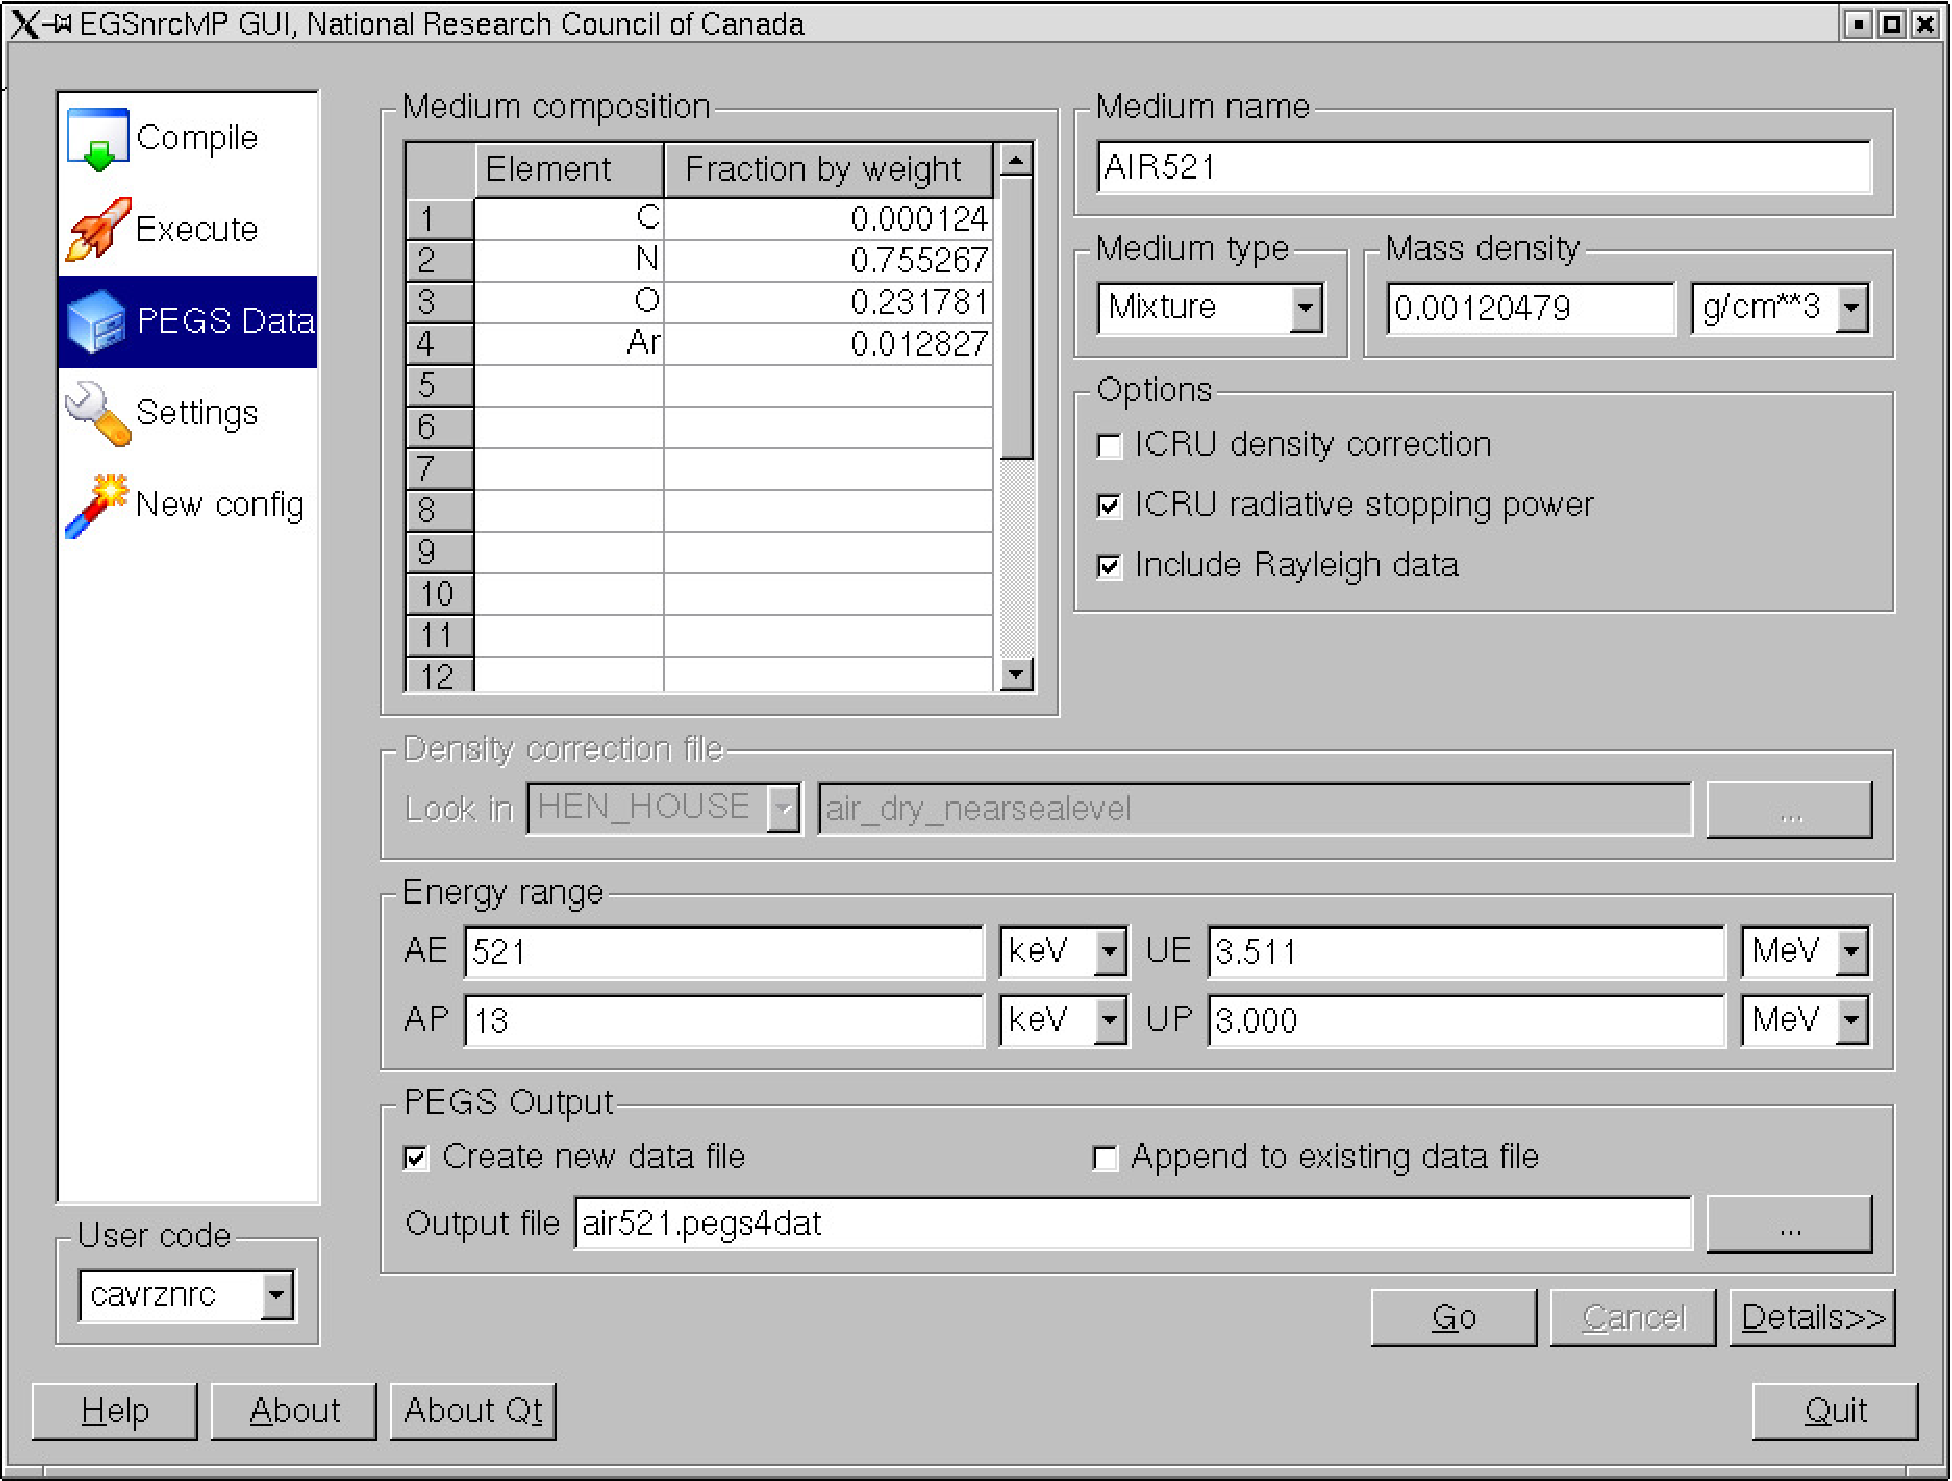
\includegraphics[width=12cm]{figures/egs_gui_pegs4_screen}
    \end{center}
   \caption{Screen shot of the {\tt egs\_gui} set to run PEGS4 to create
an air data set. Filling in this form is much easier than creating an input
file and access to the density effect corrections is easy. The GUI
does not allow any value except {\tt IUNRST = 0}. For details, see
PIRS-877\cite{Ka03}. }
   \label{fig_pegs4_screen}
\end{figure}

\subsection{Some new documentation}

\subsubsection{Photon data for EGSnrc}
\label{xsections}
Originally, EGS main field of application was high energy physics.
For this reason, no attention was paid to the accuracy of the
photon cross sections near atomic absorption edges\cite{RB90} and
PEGS4 was designed to generate a grid with a maximum number of photon
energy points, {\tt \$MXGE}, in the entire energy range requested by the user.
{\tt \$MXGE} is a macro which sets the array dimensions for the energy-dependent
photon data. Although {\tt \$MXGE} can be changed in the PEGS4 code,
PEGS4's algorithm for deciding how many bins to use might still pick many
fewer bins than {\tt \$MXGE}. The decision is based on the overall accuracy to
reproduce the cross sections in the entire energy interval.

\begin{figure}[hbtp]
\begin{center}
\includegraphics*[width=10.0cm]{figures/xcom_250keV_zoom}
\end{center}
\caption[Mean free path $\lambda$ for lead in the vicinity
of the L1 and L2 atomic absorption edges for two different
energy grids]
{Mean free path $\lambda$ for lead in the vicinity
of the L1 and L2 atomic absorption edges for two different
energy grids. Data sets generated by EGSnrc from
the XCOM cross section compilation for an energy range
10 keV to 250 keV.
}
\label{accuracy_xsections}
\end{figure}

Typical PEGS4 data sets used in radiotherapy
calculations are created for an energy range between 10 keV and 20 MeV.
If these data sets are used in the kilovoltage energy
range, inaccuracies in the cross section interpolation procedure near
absorption edges can potentially lead to errors in the calculations.
Fig. \ref{accuracy_xsections} shows two cross section data sets
for the same energy range (10 keV - 250 keV) when using
different energy grids (200 and 2000 bins). A coarser energy
grid will cause larger interpolation errors near the absorption edge.

EGSnrc default behavior has been set to ignore PEGS4 photon
data and recreate the photon cross sections using a logarithmic energy
grid with {\tt \$MXGE} energy points. However, EGSnrc still needs the
PEGS4 data file for material information, photon threshold energies
({\tt AP, UP}), and a fraction of the electron data.
By default data is read from the
Storm and Israel\cite{SI70} photon cross section compilation
({\tt si\_pair.data, si\_photo.data, si\_rayleigh.data and
si\_triplet.data}).
As alternative, EGSnrc offers such cross section data files
for the XCOM\cite{HS95} ({\tt xcom\_*.data}) and EPDL97\cite{Cu89}
({\tt epdl\_*.data}) photon cross section compilations.
New photon cross section compilations can be added following the
same format as above, \ie, {\tt prefix\_*.data}.
The choice of the photon cross section
compilation is done by input as shown in the example below:
\begin{verbatim}

  :start MC transport parameter:
      .                             # This entry is case sensitive
      Photon cross sections = xcom  # xcom, epdl, si(default) or any_prefix
      .
  :stop MC transport parameter:

\end{verbatim}
The prefix used is case sensitive and must be such that the required files
are available in the {\tt \$HEN\_HOUSE/data} directory.

Since the 2011 release (V4-r2-3-2) EGSnrc allows the
use of photon cross section data in the PEGS4 data file. This could
come in handy to compare with older calculations for validation
purposes. To accomplish this, one must set the photon cross section key to
{\tt pegs4} (case insensitive) as shown in the following input file snippet:
\begin{verbatim}

  :start MC transport parameter:
      .
      Photon cross sections = pegs4 # case insensitive
      .
  :stop MC transport parameter:

\end{verbatim}
\subsubsection{Some additional outputs- unrestricted cross sections}
The original version of PEGS4 contained a few undocumented options which
many people have made use of, so they are now documented here.  Basically
there is an additional parameter, {\tt IUNRST} which allows various stopping
powers to be calculated, rather than just the restricted stopping powers
normally calculated when {\tt IUNRST = 0}.  The {\tt IUNRST} input is made as part of
the namelist input for INP (along with NE, AE etc).  Basically {\tt IUNRST} gives
access to a variety of different stopping powers and allows for simulations
which model various types of CSDA calculations.
\begin{description}
\index{IUNRST}
\index{restricted stopping powers}
\index{unrestricted stopping powers}
\index{radiative stopping powers}
\index{collision stopping powers}
\item[IUNRST = 0, restricted stopping powers:] This is the default case
which is needed for normal simulations. The stopping powers output by PEGS4
are the restricted collision and radiative stopping powers.

\item[IUNRST = 1, unrestricted collision stopping power:] This is useful
for calculating unrestricted stopping powers for comparison to frequently
published values.

\item[IUNRST = 2, CSDA data set:] This produces a data set which can do one
form of CSDA calculation. The stopping power produced is the unrestricted
total (collision + radiative) stopping power and the distances to discrete
electron interactions is infinite (i.e. they never occur). A simulation
done with this data set is a form of CSDA calculation, with all of the
bremsstrahlung energy deposited locally.

\item[IUNRST = 3, CSDA calculation with brem interaction:] The stopping
powers are the sum of the unrestricted collision stopping power plus the
restricted stopping power and the distance to discrete interactions takes
into account only bremsstrahlung events.

\item[IUNRST = 4, CSDA calculation with delta-ray interactions:] The
stopping powers are the sum of the restricted collision stopping powers and
the unrestricted collision stopping powers and the distance to discrete
interactions takes into account only the creation of knock-on electrons
or delta-rays.

\item[IUNRST = 5, unrestricted radiative stopping power:] This complements
{\tt IUNRST = 1} and allows comparison to published radiative stopping powers.

\item[IUNRST = 6, restricted radiative stopping power:] Allows for direct
calculation of the restricted radiative stopping powers.

\item[IUNRST = 7, restricted collision stopping powers:] Allows for direct
calculation of the restricted collision stopping power.
\end{description}
Note that for low values of AP (e.g. 0.010 keV) the restricted radiative
collision stopping power is very close to zero and hence the stopping
powers with {\tt IUNRST = 0} are close to those for {\tt IUNRST = 7}.

The code EXAMIN (see section~\ref{examin}, page~\pageref{examin}) will take
the data sets produced by PEGS4 and print tables of cross section data
and/or plot these same data in user friendly units.
\index{EXAMIN}

\subsubsection{Use of ICRU Report 37 Collision Stopping Powers}
\label{icru37_csp}
\index{ICRU Report 37}
\index{collision stopping powers}
For very precise dosimetry work it is often advantageous to make use of
collision stopping powers recommended by the ICRU in their Report
37\cite{ICRU37}.  This option was added to PEGS4 in 1989\cite{Du89}.
Basically PEGS4 allows the user to read in a file which contains an arbitrary
density effect data set ($\delta$ values). The EGSnrc distribution
supplies the data sets
required for a large number of materials as calculated by Berger and
Seltzer\cite{BS83} for ICRU Report 37 (see
\verb+$HEN_HOUSE/pegs4/density_corrections+).
\index{Seltzer, Stephen} \index{Berger, Martin}

\index{PEGS4!EPSTFL}
\index{EPSTFL}
To implement this option, one adds {\tt EPSTFL=1} to the {\tt INP}
namelist input for the {\tt ELEM, COMP} or {\tt MIXT} option
and executes PEGS4 as:
\begin{verbatim}
pegs4.exe -i inputfile [-o ofile] [-a] [-d density] [-x crosssection] [-e HEN_HOUSE]

inputfile.pegs4inp   the input file
output defaults to $HEN_HOUSE/pegs4/data/inputfile.pegs4dat
                or, if ofile is given, to $HEN_HOUSE/pegs4/data/ofile.pegs4dat
[-a]            => append results to output file
[-d density]    => use density.density   for density effect
[-x crosssection] => use $HEN_HOUSE/pegs4/crosssection instead of
                                $HEN_HOUSE/pegs4/pgs4pepr.dat
[-e HEN_HOUSE]  => use this absolute location as the HEN_HOUSE
\end{verbatim}
where {\tt input1.pegs4inp} contains the standard PEGS4 input file (with
{\tt EPSTFL=1}) and {\tt  input2.density} is the file with the density effect
data needed.

PEGS4 verifies that the data in {\tt input2.density} corresponds to the same
material as described in {\tt input1.pegs4inp}, and in particular demands
that the densities match.  If you want to create a data set using the
density effect data for graphite based on a density of 2.26 g/cm$^3$ but
the real bulk data is 1.70 g/cm$^3$, you must edit the density effect file
and artificially change the density to match the bulk density you are
after, otherwise PEGS4 will stop.

Note that the density effect file also provides the ICRU 37 value of the I
value for the material and PEGS4 uses this rather than its internally
calculated value.

Data sets created with {\tt EPSTFL=1} and {\tt IUNRST = 1} should match the
collision stopping powers in ICRU Report 37 exactly.

\subsubsection{Use of ICRU Report 37 Radiative Stopping Powers}
\index{IAPRIM}
\index{radiative stopping powers}
\index{ICRU Report 37}
In 1989 an option was added to PEGS4\cite{Ro89a} which ensured that
the unrestricted radiative stopping powers calculated by PEGS4 were
identical to those calculated by Berger and Seltzer\cite{BS83} and
included in ICRU Report 37\cite{ICRU37}.  This was done by scaling the
cross sections used in PEGS4 to ensure that these stopping powers matched.
This made a significant difference to the bremsstrahlung cross sections
at low energies.  It is strongly recommended that this option always
be used and has been made the default value in PEGS4. To restore the
original PEGS4 values, enter  the input {\tt IAPRIM=0}
to the {\tt INP} namelist input for the {\tt ELEM, COMP} or {\tt MIXT}
option.
\index{PEGS4!IAPRIM}


Note that this change does not produce the same photon differential cross
sections as calculated by Seltzer and Berger\cite{SB85}, but this option
has been added to EGSnrc (see section~\ref{step_2}) and turned on by
setting {\tt ibr\_nist = 1}.
\index{ibr\_nist}



\subsubsection{A Bug in PEGS4}
\index{PEGS4!bug}
Although the PEGS4 manual reports that one may produce data sets for many
materials in one run, this is not in fact possible.  One must run the code
separately for each material desired and then concatenate these files into
one master file.

\newpage
\subsection{Original PEGS4 User Manual}
%\begin{center}
\index{Nelson, Ralph}
\index{Hirayama, Hideo}
\begin{verbatim}


                     SLAC265 - APPENDIX 3



                      PEGS4 User Manual






                              By


                       Walter R. Nelson
               Stanford Linear Accelerator Center
                      Stanford University
                   Stanford, CA 94305, U.S.A.


                        Hideo Hirayama
       National Laboratory for High Energy Physics (KEK)
            Oho-machi, Tsukuba-gun, Ibaraki, Japan


                      David W. O. Rogers
              National Research Council of Canada
                    Ottawa K1A 0R6, Canada



                       31 December 1985









      [This PEGS4 User Manual is based directly on Appendix 3 of
               SLAC-265, The EGS4 Code System]
\end{verbatim}



%\end{center}
%\end{center}
 \newpage \index{PEGS4!introduction} \begin{verbatim}
 A3.  PEGS4 USER MANUAL
 -----------------
 A3.1 Introduction
 -----------------

      The PEGS code (Preprocessor for EGS) is a stand alone
 utility program written in Mortran **.  PEGS' purpose is to
 generate material data for the EGS code, and to provide other
 services for the user who is studying or simulating electro-
 magnetic interactions.  The active operations of PEGS are
 functionals; that is, they are operations whose arguments are
 functions (the functions related to physics interactions).
 Included among these operations are:

      -  Fitting of functions by means of piecewise linear fits.

      -  Production of print plots of selected functions.

      -  Evaluation of functions at selected points.

      -  Comparision of functions with sampled spectra.


 Associated with these active functionals are other operations;
 namely,


      -  Selection of material to which the functions refer.

      -  Selection of energy cutoffs for fits.

      -  Punching of fit data.


 [Note: Those interested in preparing data sets for EGS4 can go
        directly to Section A3.3]

 ---------------
\end{verbatim}
{\tt   ** A. J. Cook, "Mortran3 User's Guide"\cite{Co83}.  Also, see
``An EGS Users Guide to Mortran3'' (section~\ref{UGM3}).}
\begin{verbatim}




 A3.1-1
\end{verbatim}
\newpage
\index{PEGS4!structure}
\begin{verbatim}
 ------------------------------------
 A3.2 Structural Organization of PEGS
 ------------------------------------
      The PEGS code contains over 4200 Mortran source lines
 which are the source for a MAIN program, BLOCK DATA subpro-
 gram, 12 subroutines, and 83 functions.  Despite the large
 number of subprograms, PEGS has a simple structure.  Fig.
 A3.2.1 shows a flowchart of the MAIN program of PEGS.  After
 the once-only initializations an option loop is entered.
 Each time through the option loop, an option is read (option
 names are four characters and are read as 4A1), numeric con-
 trol parameters are read (using NAMELIST/INP/), and then the
 option name is looked up in the option table.  If not found,
 the job is aborted.  If found, the appropriate code is exec-
 uted and return is passed to the beginning of the option
 loop.  Normal exit from the loop is by selection of the STOP
 option, or detection of an End of File condition on the con-
 trol input file.  The details for the use of the options are
 contained in Section A3.3.

      Fig. A3.2.2 shows the subprogram relationships of PEGS.
 Boxed items are subprograms, and labels for option names
 (i.e., :CALL:) are used to show which subprograms correspond to
 which options.  It can be seen that the physical routines are
 accessed directly for the PWLF option.  For utility options
 (TEST, PLTN, PLTI, HPLT, and CALL) the physical routines are
 referenced using the function FI---the so-called "function
 multiplexer".  Function FI has five arguments.  The first
 argument (I) tells which physical function to invoke, and the
 other four arguments (X1, X2, X3, X4) are used as needed as
 arguments for the called function.  FI then returns the value
 returned by the called function.

      This method of implementing options that are functionals
 was selected to avoid the necessity of having a separate call
 to the associated utility routines for each physical function
 on which it might be desired to operate.  It was also desired
 to be able to refer to the particular function symbolically,
 both at compile time and at run-time, and to know the number
 of arguments to each function.  In order to have these
 conveniences and also allow easy insertion or deletion of
 functions to the list of functions accessible to FI, a
 Mortran macro ($FUNCTIONS) was written which takes a
 list of names of functions (each of which is immediately pre-
 ceded by the number of arguments it has) and generates other
 macros containing the desired information.  In particular,
 A3.2-1
\end{verbatim}
\newpage
\index{PEGS4!flow chart}
\begin{center}
\begin{boxedverbatim}
                          +------+
                          | PEGS |
                          +------+
                            |  |       +-------------+
                initialize  |  +------>| OPTION LOOP |<-----+
             +--------------+          +-------------+      A
             |                                |             |
             |                                |             |
             V                                V             |
 +------------------------+          +-----------------+    |
 |   Compute Physical &   |          |   Read Option   |    |
 | Mathematical Constants |          |    Name (4A1)   |    |
 +------------------------+          |        &        |    |
             |                       |   Read Control  |    |
             |                       |    Parameters   |    |
             V                       | (NAMELIST/INP/) |    |
 +------------------------+          +-----------------+    |
 | Read Pair Production & |                   |             |
 |  Photo Cross Sections  |                   |             |
 |    from File PHPRDAT   |                   |             |
 +------------------------+                   |             |
                                              V             |
                +------+     Yes      +--------------+      |
                | Stop |<------------ | End of File? |      |
                +------+              +--------------+      |
                                              |             |
                                              | No          |
                                              |             |
                                              V             |
      +-----------------------+       +---------------+     |
      | Illegal Option---Stop |<----- | Select Option |     |
      +-----------------------+       +---------------+     |
                                              |             |
                                              |             |
                                              V             |
   +<---------------------------------------- +             |
   |                                                        |
   V                                                        |
   *                                                        *
  * *                                                      * *
 * 1 *                                                    * 2 *
  * *                                                      * *
   *                                                        *
      Fig. A3.2.1  Flowchart of the MAIN Program of PEGS
                        (continued on next page)
 A3.2-2
\end{boxedverbatim}
\end{center}
\newpage \index{PEGS4!flow chart}
\begin{center}
\begin{boxedverbatim}
   *                                                         *
  * *                                                       * *
 * 1 *                                                     * 2 *
  * *                                                       * *
   *                                                         *
   |          +-----------------------+                      ^
   +-->:ELEM: | Set Up Element Medium | -------------------> |
   |          +-----------------------+                      |
   |          +-----------------------+                      |
   +-->:MIXT: | Set Up Mixture Medium | -------------------> |
   |          +-----------------------+                      |
   |          +------------------------+                     |
   +-->:COMP: | Set Up Compound Medium | ------------------> |
   |          +------------------------+                     |
   |          +------------------------+                     |
   +-->:ENER: | Set Energy Cutoffs and | ------------------> |
   |          | Compute Thresholds     |                     |
   |          +------------------------+                     |
   |          +---------------------+                        |
   +-->:PLTN: | Plot Named Function | ---------------------> |
   |          +---------------------+                        |
   |          +-----------------------+                      |
   +-->:PLTI: | Plot Indexed Function | -------------------> |
   |          +-----------------------+                      |
   |          +-----------------------+                      |
   +-->:HPLT: | Histogram Theoretical | -------------------> |
   |          |  vs Sampled Spectrum  |                      |
   |          +-----------------------+                      |
   |          +-------------------------+                    |
   +-->:CALL: | Evaluate Named Function | -----------------> |
   |          +-------------------------+                    |
   |          +-----------------------------+                |
   +-->:TEST: | Plot Functions To Be Fitted | -------------> |
   |          +-----------------------------+                |
   |          +----------------------+                       |
   +-->:PWLF: | Piecewise Linear Fit | --------------------> |
   |          +----------------------+                       |
   |          +------------------------+                     |
   +-->:DECK: | Punch Deck of Material | ------------------> +
   |          | Dependent Data         |
   |          +------------------------+
   |          +------+
   +-->:STOP: | Stop |
              +------+
      Fig. A3.2.1  Flowchart of the MAIN Program of PEGS
                     (continued from previous page)
 A3.2-3
\end{boxedverbatim}
\end{center}
\newpage \index{PEGS4!subprograms}
\begin{center}
\begin{boxedverbatim}
     +------------+         +------+
     | BLOCK DATA |         | MAIN |
     +------------+         +------+
                                |
     + --- + -- + ----- + ----- + ----- + ----- + ---- + ---- +
     |     |            |       |       |       |      |      |
     |     |         :PWLF:  :DECK:  :TEST:  :HPLT: :CALL: :ENER:
     |     |            |       |    :PLTN:     |      |
     |     |            |     +---+  :PLTI:  +-----+   |
     |     |            |     |LAY|     |    |HPLT1|   |
     |     |            |     +---+     |    +-----+   |
     |     |            |            +----+     |      |
  +------+ |        +---+----+       |PLOT|     |      |
  |PMDCON| |        |        |       +----+     |      |
  +------+ |     +-----+  +-----+       |       |      |
           |     |EBIND|  |PWLF1|       +-----> | <--- +
           |     +-----+  +-----+               |
        :ELEM:               |                  |
        :MIXT:            +----+                |
        :COMP:            |QFIT|                *
           |              +----+               * *
   + ----- + ----- +         |                * 3 *
   |       |       |         |                 * *
 +---+ +------+ +------+     |                  *
 |MIX| |SPINIT| |DIFFER|     |
 +---+ +------+ +------+     |
                        + -- + -- + --------------- +
                        |         |                 |
                     +-----+   +-----+           +-----+
                     |EFUNS|   |GFUNS|           |RFUNS|
                     +-----+   +-----+           +-----+
                        |         |                 |
    +-----+----+-----+--+---+---+ |   +------+   +-----+
    |     |    |     |      |   | +---|PHOTTE|   |AINTP|
 +------+ | +------+ | +------+ | |   +------+   +-----+
 |SPTOTP| | |ANIHTM| | |BHABTM| | |   +------+
 +------+ | +------+ | +------+ | +---|COMPTM|
          |          |          | |   +------+
 +------+ | +------+ | +------+ | |   +------+
 |SPTOTE|-+ |AMOLTM|-+ |BREMTM|-+ +---|PAIRTU|
 +------+   +------+   +------+   |   +------+
                                  |   +------+
                                  +---|COHETM|
                                      +------+
      Fig. A3.2.2  Subprogram Relationships of PEGS
                      (continued on next page)
 A3.2-4
\end{boxedverbatim}
\end{center}
\newpage \index{PEGS4!subroutines}
\begin{center}
\begin{boxedverbatim}
                               *
                              * *
                             * 3 *
                              * *
                               *
                               |
                               |
                               |
                               |
                  + ---------------------- +
                  |           FI           |
                  | "Function Multiplexer" |
                  + ---------------------- +
                               |
                               |
                               |
           + ------------------------------------- +
           |                                       |
           |   ALIN     APRIM    COMPFM   PAIRTE   |
           |   ALINI    BHABDM   COMPRM   PAIRTM   |
           |            BHABFM   COMPTM   PAIRTR   |
           |   ADFMOL   BHABRM   CRATIO   PAIRTU   |
           |   ADIMOL   BHABTM   EBIND    PAIRTZ   |
           |   ADDMOL   BREMDR   EBR1     PBR1     |
           |   ALOG     BREMFR   EDEDX    PBR2     |
           |   EXP      BREMDZ   ESIG     PDEDX    |
           |   AREC     BRMSDZ   FCOULC   PHOTTZ   |
           |   ALKE     BREMFZ   GBR1     PHOTTE   |
           |   ALKEI    BRMSFZ   GBR2     PSIG     |
           |   AMOLDM   BREMRR   GMFP     SPIONE   |
           |   AMOLFM   BREMRM   PAIRDR   SPIONP   |
           |   AMOLRM   BREMRZ   PAIRFR   SPTOTE   |
           |   AMOLTM   BREMTM   PAIRDZ   SPTOTP   |
           |   ANIHDM   BREMTR   PAIRFZ   TMXB     |
           |   ANIHFM   BRMSRM   PAIRRM   TMXS     |
           |   ANIHRM   BRMSRZ   PAIRRR   TMXDE2   |
           |   ANIHTM   BRMSTM   PAIRRZ   XSIF     |
           |            COHETM                     |
           |            COHETZ                     |
           |            COMPDM                     |
           + ------------------------------------- +

      Fig. A3.2.2  Subprogram Relationships of PEGS
                   (continued from previous page)


 A3.2-5                                                       .
\end{boxedverbatim}
\end{center}
\newpage \index{PEGS4!macros} \begin{verbatim}
 the following macros are defined:

      $NFUNS  -  Gives the number of functions.

      $FLIST$DATA(FNAME)  -  Generates a data statement init-
      ializing the array FNAME(6,$NFUNS) so that FNAME(i,j) has
      the ith character of the name of the jth function.

      $FLIST$NARGS  -  Gives a list of the number of arguments
      for each function, which is used to initialize the run-
      time array NFARG($NFUNS).

      $FLIST$FNUMS  -  Gives a list of numbers from 1 to
      $NFUNS, which is used to generate the computed GO TO
      in FI.

      $FLIST$FCALLS  -  Generates the function calls in FI with
      the proper number of arguments for each function taken
      from the list X1, X2, X3, X4.

      $FN(function name)  -  Gives the function index of the
      specified function.

      $NA(function name)  -  Gives the number of arguments for
      the specified function.


      It should also be noted that there are relationships
 between the functions shown in Fig. A3.2.2 that are not
 indicated there.  We show the most complicated of these in
 Figs. A3.2.3a,b (Bremsstrahlung Related Functions) and in
 Figs. A3.2.4a,b (Pair Production Related Functions).  One
 reason for the complexity of these is that the higher level
 forms of the cross sections must be obtained by numerical
 integration of the more differential forms.











 A3.2-6
\end{verbatim}
\newpage \index{PEGS4!functions}
\begin{center}
\begin{boxedverbatim}
                        +------+
                        |BREMTM|
                        +------+
                            |
                            V
                        +------+
                        |BREMRM|
                        +------+
                            |
                            V
 +------+               +------+  initialize   +------+
 |  QD  |<------------- |BREMRZ|-------------> |BREMDZ|
 +------+               +------+    BREMFZ     +------+
    |                                              |
    V                                              |
 +------+                                          |
 |DCADRE|                                          |
 +------+                                          |
    |                                              |
    V                                              V
 +------+               +------+               +------+
 |BREMFZ|-------------> |BRMSFZ|<------------- |BRMSDZ|
 +------+               +------+               +------+
                            A                    A |
                            |                    | |   +------+
            +---------------+                    | +-->|APRIM |
            |                                    | |   +------+
        +------+        +------+   initialize    | |
        |DCADRE|   +----|BRMSRZ|---------------> + |   +------+
        +------+   |    +------+     BRMSFZ        +-->| XSIF |
            A      |        A                      |   +------+
            |      |        |                      |
        +------+   |    +------+                   |   +------+
        |  QD  |<--+    |BRMSRM|                   +-->|FCOULC|
        +------+        +------+                       +------+
                            |
   +------+             +------+             +------+
   |SPTOTE|-----------> |BRMSTM|<----------- |SPTOTP|
   +------+             +------+             +------+
      |                                          |
      V                                          V
   +------+             +------+             +------+
   |SPIONE|-----------> |SPIONB|<----------- |SPIONP|
   +------+             +------+             +------+
Fig. A3.2.3a  Bremsstrahlung Related Functions---Most Accurate Form
   (Used to Produce the Total Cross Sections and Stopping Power).
 A3.2-7
\end{boxedverbatim}
\end{center}
\newpage \index{PEGS4!functions}
\begin{center}
\begin{boxedverbatim}




                             +------+
                             |BREMTR|
                             +------+
                                 |
                                 |
                                 V
                             +------+
                             |BREMRR|
                             +------+
                                 |
                                 |
                      initialize V
                     + <---------+--------> +
                     |  BREMFR              |
                     |                      |
                     V                      V
                  +------+              +------+
                  |BREMDR|              |  QD  |
                  +------+              +------+
                     |                      |
                     |                      |
                     |                      V
                     |                  +------+
                     |                  |DCADRE|
                     |                  +------+
                     |                      |
                     |                      |
                     |                      |
                     |       +------+       |
                     + ----> |BREMFR| <---- +
                             +------+


     Fig. A3.2.3b  Bremsstrahlung Related Functions---With Run-
                     Time Approximations (For Comparison
                           with Sampled Spectra).






 A3.2-8
\end{boxedverbatim}
\end{center}
\newpage \index{PEGS4!functions}
\begin{center}
\begin{boxedverbatim}




                         +------+
                         |PAIRTU|
                         +------+
                           |  |
    + <------------------- +  + -------------------> +
    |                                                |
    V                                                V
 +------+                                        +------+
 |PAIRTM|                                        |PAIRTE|
 +------+                                        +------+
    |                                                |
    V                                                V
 +------+                                        +------+
 |PAIRRM|                                        |PAIRTZ|
 +------+                                        +------+
    |                                                |
    V                                                V
 +------+   initialize                           +------+
 |PAIRRZ|-------------> +                        |AINTP |
 +------+     PAIRFZ    |                        +------+
    |                   |
    |                   |
    |                   |
    |                   |
    V                   V
 +------+            +------+            +------+
 |  QD  |            |PAIRDZ|-----+----> | XSIF |
 +------+            +------+     |      +------+
   |                    |         |
   |                    |         |      +------+
   |                    |         +----> |FCOULC|
   V                    V                +------+
 +------+            +------+
 |DCADRE|----------> |PAIRFZ|
 +------+            +------+


     Fig. A3.2.4a  Pair Production Related Functions---Most
                  Accurate Form (Used to Produce the Total
                  Cross Sections and Stopping Power).


 A3.2-9
\end{boxedverbatim}
\end{center}
\newpage \index{PEGS4!functions}
\begin{center}
\begin{boxedverbatim}



                             +------+
                             |PAIRTR|
                             +------+
                                 |
                                 |
                                 V
                             +------+
                             |PAIRRR|
                             +------+
                                 |
                                 |
                      initialize V
                     + <-------- + -------> +
                     |  PAIRFR              |
                     |                      |
                     V                      V
                  +------+              +------+
                  |PAIRDR|              |  QD  |
                  +------+              +------+
                     |                      |
                     |                      |
                     |                      V
                     |                  +------+
                     |                  |DCADRE|
                     |                  +------+
                     |                      |
                     |                      |
                     |                      |
                     |       +------+       |
                     + ----> |PAIRFR| <---- +
                             +------+


     Fig. A3.2.4b  Pair Production Related Functions---With
                  Run-Time Approximations (For Comparison
                  with Sampled Spectra).







 A3.2-10
\end{boxedverbatim}
\end{center}
\newpage \index{PEGS4!subroutines} \begin{verbatim}
      Table A3.2.1 lists the SUBROUTINES used in PEGS.  A brief
 description of their use and page references for a fuller
 discussion is given.

      Table A3.2.2 lists the FUNCTIONS used in PEGS along with
 their mathematical symbols, definitions, and locations in this
 report for a fuller discussion.  The names of most of the
 functions have been chosen in a rather mnemonic way.  The
 first three or four letters suggest the process being con-
 sidered.  The last letter designates the form of the cross
 section (Z for element, M for mixture, and R for "run-time"
 mixture).  The next to last letter describes either the part-
 icular form of the cross section (such as D for differential,
 T for total or R for range-integrated), or it indicates that
 only the secondary energy is to vary, with other data being
 passed through a common.  The letter F is used in such cases
 and the data in common is initialized using the corresponding
 function that has a next to last letter of D.  If the function
 word begins with an I through N (i.e., the FORTRAN integer
 convention) the word is prefixed with the letter A.  A few
 examples are given below:


    AMOLDM is the differential Moller cross section for a
           mixture of elements.

    BREMDR is the differential bremsstrahlung cross section
           for a "run-time" mixture of elements.

    BREMRM is the bremsstrahlung cross section, integrated
           over some energy range, for a mixture of elements.

    BRMSTM is the soft bremsstrahlung total cross section for
           a mixture of elements.

    PAIRRR is the pair production cross section, integrated
           over some energy range, for a "run-time" mixture
           of elements.

    PAIRTZ is the total cross section for pair production
           for an element.

      This method of naming is not strictly adhered to,
 however.  For example, SPIONE is the ionization stopping
 power for an electron, PBR1 and PBR2 are positron branching
 ratios, and GMFP is the gamma-ray mean free path.
 A3.2-11
\end{verbatim}
\newpage \index{PEGS4!subroutines} \begin{verbatim}
                         Table A3.2.1
                   SUBROUTINES Used In PEGS
 -----------------------------------------------------------------
    NAME                 DESCRIPTION                   PAGES
 -----------------------------------------------------------------
    DIFFER    Determines the various parameters       A3.2-4,
              needed for bremsstrahlung and pair      A3.3-11
              production energy sampling.

    EFUNS     Subprogram to compute electron          A3.2-4
              functions to be fit in a way
              that avoids repetition.

    GFUNS     Subprogram to compute photon            A3.2-4
              functions to be fit in a way
              that avoids repetition.

    HPLT1     Creates line printer plot comparisons   A3.2-4,
              of EGS-sampled data (UCTESTSR User      A3.3-20,21
              Code) and theoretical functions of PEGS.

    LAY       Subprogram to produce a deck of         A3.2-4,
              material dependent data (for sub-       A3.3-17
              sequent use by EGS).

    MIX       Computes Z-dependent paramaters         A3.2-4,
              that reside in COMMON/MOLVAR/.          A3.3-11

    MOLIER    Computes material independent           A3.2-4
              multiple scattering data (EGS2 only!).

    PLOT      Subprogram to plot a given function     A3.2-4
              (referenced by number).

    PMDCON    Determines the physical, mathematical,  A3.2-4
              & derived constants in a mnemonic way.

    PWLF1     Subprogram to piecewise linearly fit    A3.2-4,19,
              up to 10 functions simultaneously on    A3.3-14
              an interval (XL,XU).

    RFUNS     Subprogram to compute Rayleigh          A3.2-4
              scattering functions to be fit in
              a way that avoids repetition.
    SPINIT    Initializes stopping power functions    A3.2-4,
              for a particular medium.                A3.3-11
 A3.2-12
\end{verbatim}
\newpage  \index{PEGS4!functions} \begin{verbatim}


                         Table A3.2.2

                   FUNCTIONS Used In PEGS


 -----------------------------------------------------------------
    NAME                 DESCRIPTION                   PAGES
 -----------------------------------------------------------------
    AFFACT    Atomic form factor (squared) for an
              element or mixture of elements.

    AINTP     Linear or log interpolation function.   A3.2-4,9

    ALKE      Log of kinetic energy (ALOG(E-RM)),     A3.2-5,
              used as a cumulative distribution       A3.3-20
              function for fits and plots.

    ALKEI     Inverse of ALKE (=EXP(X)+RM).           A3.2-5

    ALIN      Linear cumulative distribution func-    A3.2-5,
              tion for plots (ALIN(X)=X).             A3.3-20

    ALINI     Inverse of ALIN (=same as ALIN).        A3.2-5
              Used as inverse cumulative distri-
              bution function in plots.

    ADFMOL    Approximate cumulative distribution     A3.2-5,
              function for Moller and Bhabha cross    A3.3-20
              sections (ADFMOL(E)=-1/(E-RM)).

    ADIMOL    Inverse of ADFMOL.                      A3.2-5

    ADDMOL    Derivative of ADFMOL.                   A3.2-5

    AMOLDM    Moller differential cross section for   A3.2-5,11,14
              a mixture of elements.






                   (continued on next page)
 A3.2-13
\end{verbatim}
\newpage \index{PEGS4!functions} \begin{verbatim}


                         Table A3.2.2
                         (continued)


                   FUNCTIONS Used In PEGS

 -----------------------------------------------------------------
    NAME                 DESCRIPTION                   PAGES
 -----------------------------------------------------------------
    AMOLFM    "One argument" form of AMOLDM.          A3.2-5

    AMOLRM    Moller cross section, integrated over   A3.2-5
              some energy range, for a mixture of
              elements.

    AMOLTM    Moller total cross section for a        A3.2-4,5
              mixture of elements.

    ANIHDM    Annihilation differential cross         A3.2-5
              section for a mixture of elements.

    ANIHFM    "One argument" form of ANIHDM.          A3.2-5

    ANIHRM    Annihilation cross section, integrated  A3.2-5
              over some energy range, for a mixture
              of elements.

    ANIHTM    Annihilation total cross section for    A3.2-4,5
              a mixture of elements.

    APRIM     Empirical correction factor in          A3.2-5,7
              bremsstrahlung cross section.

    AREC      Reciprocal function (=derivative of     A3.2-5
              ALOG(X)).  Used as probability density
              function in log plots (AREC(X)=1/X).

    BHABDM    Bhabha differential cross section for   A3.2-5
              a mixture of elements.

    BHABFM    "One argument" form of BHABDM.          A3.2-5


                   (continued on next page)
 A3.2-14
\end{verbatim}
\newpage  \index{PEGS4!functions}\begin{verbatim}

                         Table A3.2.2
                         (continued)

                   FUNCTIONS Used In PEGS
 -----------------------------------------------------------------
    NAME                 DESCRIPTION                   PAGES
 -----------------------------------------------------------------
    BHABRM    Bhabha cross section, integrated over   A3.2-5
              some energy range, for a mixture of
              elements.

    BHABTM    Bhabha total cross section for a        A3.2-4,5
              mixture of elements.

    BREMDR    Bremsstrahlung differential cross       A3.2,5,8,11
              section for a "run-time" mixture
              of elements.

    BREMFR    "One argument" form of BREMDR.          A3.2-5,8

    BREMDZ    Bremsstrahlung differential cross       A3.2-5,7
              section for an element.

    BREMFZ    "One argument" form of BREMDZ.          A3.2-5,7

    BREMRM    Bremsstrahlung cross section, inte-     A3.2-5,7,11
              grated over some energy range, for a
              mixture of elements.

    BREMRR    Bremsstrahlung cross section, inte-     A3.2-5,8
              grated over some energy range, for a
              "run-time" mixture of elements.

    BREMRZ    Bremsstrahlung cross section, inte-     A3.2-5,7
              grated over some energy range, for an
              element.

    BREMTM    Bremsstrahlung total cross section      A3.2-4,5,7
              for a mixture of elements.

    BREMTR    Bremsstrahlung total cross section      A3.2-5,8
              for a "run-time" mixture of elements.

                   (continued on next page)
 A3.2-15
\end{verbatim}
\newpage  \index{PEGS4!functions}\begin{verbatim}
                        Table A3.2.2
                         (continued)
                   FUNCTIONS Used In PEGS
 -----------------------------------------------------------------
    NAME                 DESCRIPTION                   PAGES
 -----------------------------------------------------------------
    BRMSDZ    Soft bremsstrahlung differential        A3.2-5,7
              cross section for an element.

    BRMSFZ    "One argument" form of BRMSDZ.          A3.2-5,7

    BRMSRM    Soft bremsstrahlung cross section,      A3.2-5,7
              integrated over some energy range, for
              a mixture of elements.

    BRMSRZ    Soft brems cross section integrated     A3.2-5,7,
              over an energy range,for an element.    A3.3-19,20

    BRMSTM    Soft bremsstrahlung total cross         A3.2-5,7,11
              section for a mixture of elements.

    COHERTM   Coherent (Rayleigh) total cross         A3.2-4,5
              section for a mixture of elements.

    COHETZ    Coherent (Rayleigh) total cross         A3.2-5
              section for an element.

    COMPDM    Compton differential cross section      A3.2-5
              for a mixture of elements.

    COMPFM    "One argument" form for COMPDM.         A3.2-5

    COMPRM    Compton cross section, integrated over  A3.2-5
              an energy range, for a mixture of elements.

    COMPTM    Compton total cross section for a       A3.2-4,5
              mixture of elements.

    CRATIO    Coherent (Rayleigh) cross section ratio A3.2-5

    DCADRE    Quadrature routine to integrate f(x)    A3.2-7-10,19
              from a->b by cautious Romberg extrapolation.

    EBIND     Function to get an average photo-       A3.2-4,5
              electric binding energy.
                   (continued on next page)
 A3.2-16
\end{verbatim}
\newpage \index{PEGS4!functions} \begin{verbatim}
                        Table A3.2.2
                         (continued)

                   FUNCTIONS Used In PEGS
 -----------------------------------------------------------------
    NAME                 DESCRIPTION                   PAGES
 -----------------------------------------------------------------

    EBR1      Function to determine the electron(-)   A3.2-5
              branching ratio (Brem/Total).

    EDEDX     Evaluates SPTOTE with cutoff energies   A3.2-5
              of AE and AP.

    ESIG      Determines the total electron(-)        A3.2-5
              interaction cross section (prob-
              ability per radiation length).

    FCOULC    Coulomb correction term in pair         A3.2-5,7,9
              production and bremsstrahlung cross
              sections.

    FI        Function multiplexer.                   A3.2-1,5,6

    GBR1      Function to determine the gamma-ray     A3.2-5
              branching ratio (Pair/Total).

    GBR2      Function to determine the gamma-ray     A3.2-5
              branching ratio ((Pair+Compton)/Total).

    GMFP      Function to determine the gamma-ray     A3.2-5,11,
              mean free path.                         A3.3-18,19

    IFUNT     Given PEGS function name, it looks it
              up name in table and returns the
              function index.  Used by options that
              specify functions by name.

    PAIRDR    Pair production differential cross      A3.2-5,10,18
              section for a "run-time" mixture of
              elements.

    PAIRDZ    Pair production differential cross      A3.2-5,9,18
              section for an element.

                   (continued on next page)
 A3.2-17
\end{verbatim}
\newpage \index{PEGS4!functions} \begin{verbatim}
                         Table A3.2.2
                         (continued)
                   FUNCTIONS Used In PEGS
 -----------------------------------------------------------------
    NAME                 DESCRIPTION                   PAGES
 -----------------------------------------------------------------
    PAIRFR    "One argument" form of PAIRDR.          A3.2-5,10
    PAIRFZ    "One argument" form of PAIRDZ.          A3.2-5,10

    PAIRRM    Pair production cross section, inte-    A3.2-5,9
              grated over some energy range, for a
              mixture of elements.

    PAIRRR    Pair production cross section, inte-    A3.2-5,10,11
              grated over some energy range, for a
              "run-time" mixture of elements.

    PAIRRZ    Pair production cross section, inte-    A3.2-5,9
              grated over energy range, for element.

    PAIRTE    "Empirical" total pair production       A3.2-5,9
              production cross section for a
              mixture (=SUM(PZ(I)*PAIRTZ(Z(I))).

    PAIRTM    Pair production total cross section     A3.2-5,9
              for a mixture of elements, obtained
              by numerical integration of differ-
              ential cross section.

    PAIRTR    Pair production total cross section     A3.2-5,10
              for a "run-time" mixture of elements.

    PAIRTU    Pair production total cross section     A3.2-4,5,9
              actually "used".  Same as PAIRTE for
              primary energy less than 50 MeV;
              otherwise, same as PAIRTM.

    PAIRTZ    Computes contribution to empirical      A3.2-5,9,11
              pair production total cross section
              for an element assuming one atom per
              molecule.  It is obtained by log-linear
              interpolation of Israel-Storm data.

    PBR1      Function to determine the positron      A3.2-5,11
              branching ratio (Brem/Total).
                   (continued on next page)
 A3.2-18
\end{verbatim}
\newpage \index{PEGS4!functions} \begin{verbatim}
                         Table A3.2.2
                         (continued)
                   FUNCTIONS Used In PEGS
 -----------------------------------------------------------------
    NAME                 DESCRIPTION                   PAGES
 -----------------------------------------------------------------
    PBR2      Function to determine the positron      A3.2-5,11
              branching ratio ((Brem+Bhabha)/Total).

    PDEDX     Evaluates SPTOTP with cutoff energies   A3.2-5
              of AE and AP.

    PHOTTE    Determines the proper mix of PHOTTZ's   A3.2-4,5
              for a mixture.

    PHOTTZ    Determines the interpolated total       A3.2-5
              photoelectric cross section from
              tabulated data.

    PSIG      Determines the total positron           A3.2-5
              interaction cross section (prob-
              ability per radiation length).

    QD        Driver function for DCADRE, the         A3.2-7-10
              numerical integration routine.

    QFIT      Utility logical function for the        A3.2-4,
              piecewise linear fit subroutine, PWLF1. A3.3-14,15
              It returns .TRUE. if a given parti-
              tion gives a good fit.

    SPIONB    Does the work for SPIONE and SPIONP.    A3.2-7
              One argument tells whether to compute
              stopping power for electron or positron.

    SPIONE    Calculates the stopping power due to    A3.2-5,7
              ionization for electrons(-).

    SPIONP    Calculates the stopping power due to    A3.2-5,7
              ionization for positrons.

    SPTOTE    Calculates the total stopping power     A3.2-4,5,7
              (ionization plus soft bremsstrahlung)
              for electrons(-) for specified cutoffs.

                   (continued on next page)
 A3.2-19
\end{verbatim}
\newpage  \index{PEGS4!functions}\begin{verbatim}


                         Table A3.2.2
                         (continued)

                   FUNCTIONS Used In PEGS

 -----------------------------------------------------------------
    NAME                 DESCRIPTION                   PAGES
 -----------------------------------------------------------------
    SPTOTP    Calculates the total stopping power     A3.2-4,5,7,19
              (ionization plus soft bremsstrahlung)
              for positrons for specified cutoffs.

    TMXB      Determines the maximum total step       A3.2-5
              length consistent with Bethe's
              criterion.

    TMXS      Determines the minimum of TMXB and      A3.2-5
              10 radiation lengths.

    TMXDE2    Included for possible future modifi-    A3.2-5
              cation purposes (=TMXB/(E**2*BETA**4)).
              It might be easier to fit this quantity
              than to fit TMXB and then apply the
              the denominator in EGS at run-time.

    XSIF      Function to account for bremsstrahlung  A3.2-5,7,9
              and pair production in the field of
              the atomic electrons.

    ZTBL      Given the atomic symbol for an element,
              it returns the atomic number.













 A3.2-20                                                APPENDIX 3
\end{verbatim}
\newpage \index{PEGS4!options} \index{PEGS4!inputs}
\index{PEGS4!ELEM option}  \index{PEGS4!COMPT option} \index{PEGS4!MIXT option}
\label{pegs4_input}
\begin{verbatim}
 ------------------------------------------
 A3.3 PEGS Options and Input Specifications
 ------------------------------------------
    -------------------------------------
    A3.3.1 Interrelations Between Options
    -------------------------------------

      Fig. A3.3.1 illustrates the logical relationship between options of
PEGS.  For example, in order to be able to use the PLTN option, one of the
material specification options (ELEM, MIXT, COMP) must have already been
processed.  The PWLF option requires that both the ENER option and one of
the material specification options precede it.  To use the DECK option, it
is sufficient to have validly invoked the PWLF option.  The STOP and MIMS
options are seen to be independent of the others.

      In the following sections, for each option we will give its function,
parameters which control it, the format of cards needed to invoke it, and
an explanation of the routines (if any) that are used to implement it.  The
cards for a given option are named with the first part of their name being
the option name, and the last part the card number.  For example, MIXT2 is
the name of the second card needed for the MIXT option.  The information is
summarized in Table A3.3.1.  It should be noted that IBM and CDC require
different formats for NAMELIST data.  Also, the single card referred to as
being read by NAMELIST may in fact be several cards, provided that the
proper convention for continuing NAMELIST cards is followed.  Once the
first card (indicating the option) has been read in, however, the second
card (i.e., NAMELIST/INP/) must follow (see examples at the end of Section
A3.3.2).  We will use the IBM form of NAMELIST in our examples.

 -----------------------------------
 A3.3.2 The ELEM, MIXT, COMP Options
 -----------------------------------

      The purpose of the ELEMent, MIXTure, and COMPound options is to
specify the material used by the PEGS functions.  The parameters needed to
specify a material are its density (RHO), the number of different kinds of
atoms (NE), and, for each different kind of atom, its atomic number (Z(I)),
its atomic weight (WA(I)), and its proportion either by number (PZ(I)) for
a compound or by weight (RHOZ(I)) for a mixture.  PEGS has tables for the
atomic symbol (ASYMT(1:100)) and the atomic weight (WATBL(1:100)) for
elements I=1 through I=100, so the type of atom is specified by giving its
atomic symbol (ASYM(I)).  PEGS also has a table of the densities of the
elements (RHOTBL(1:100)).  Rayleigh (coherent) scattering data will be
appended to the normal output data if the IRAYL flag is set to 1 in
NAMELIST/INP/.

 A3.3-1
\end{verbatim}
\newpage \index{PEGS4!options}
\begin{center}
\begin{boxedverbatim}


   +------+    +------+    +------+          +------+
   |:ELEM:|    |:MIXT:|    |:COMP:|          |:ENER:|
   +------+    +------+    +------+          +------+
       |          |           |                  |
       |          |           |                  |
       |          |           |                  |
       |          V           |                  |
       |                      |                  |
       + ------> OR <-------- +                  |
                                                 |
                  |                              V
                  |
                  +---------------------------> AND ----+
                  |                                     |
                  |                              |      |
                  V                              |      |
    + -------+----+----+------- +                |      |
    |        |         |        |                |      |
    |        |         |        |                |      |
    V        V         V        V                |      |
 +------+ +------+ +------+ +------+ +------+    |      |
 |:PLTN:| |:PLTI:| |:HPLT:| |:CALL:| |:TEST:|<---+      |
 +------+ +------+ +------+ +------+ +------+           |
                                                        |
                                                        V
                                                     +------+
                                                     |:PWLF:|
 +------+                                            +------+
 |:MIMS:|                                               |
 +------+                                               |
                                                        V
 +------+                                            +------+
 |:STOP:|                                            |:DECK:|
 +------+                                            +------+





           Fig. A3.3.1  Logical Relationship Between
                       the Options of PEGS



 A3.3-2                                                 APPENDIX 3
\end{boxedverbatim}
\end{center}
\newpage \index{PEGS4!inputs}\index{ISSB} \begin{verbatim}
                         Table A3.3.1
                     PEGS Control Cards
 -----------------------------------------------------------------------
  CARD    FORMAT    VARIABLES READ          COMMENTS
 -----------------------------------------------------------------------
  ELEM1   (4A1)        OPT(1:4)    'ELEM'.  Means "select mat-
                                   erial that is an element."

  ELEM2 NAMELIST/INP/    RHO       Optional.  If given, this
                                   over-rides the PEGS default
                                   density (g/cm**3) for the element.

                         WA(1)     Optional.  Atomic weight of
                                   element.  If given, this
                                   over-rides the PEGS default.
                        IRAYL      Optional.  Set to unity to

                                   included Rayleigh output.

                        IUNRST     Optional.  Set to unity for
                                   unrestricted collision stopping power.

                        ISSB       Optional.  Set to unity to
                                   use own density effect param-
                                   eters (see text below).
                        GASP       Optional. See MIXT or COMP

  ELEM3 (24A1,       MEDIUM(1:24)  Identifier assigned to data
         6X,24A1)                  set to be produced.

                     IDSTRN(1:24)  Optional.  Identifer of
                                   medium name under which
                                   desired Sternheimer-Seltzer-
                                   Berger coeffcients are given
                                   in PEGS.  If not specified,
                                   identifier in MEDIUM(1:24) is used.

  ELEM4 (24(A2,1X))    ASYM(1)     Atomic symbol for element.
 -----------------------------------------------------------------------
  COMP1   (4A1)        OPT(1:4)    'COMP'.  Means "select mat-
                                   erial that is a compound."

  COMP2 NAMELIST/INP/    NE        Number of elements in compound.

                        RHO        Density (g/cm**3) of compound
                                   (at NTP for gases).
 A3.3-3                  (continued on next page)
\end{verbatim}
\newpage \index{PEGS4!inputs} \begin{verbatim}
                         Table A3.3.1
                         (continued)
                     PEGS Control Cards
 -----------------------------------------------------------------
  CARD    FORMAT   VARIABLES READ          COMMENTS
 -----------------------------------------------------------------
                   (PZ(I),I=1,NE)  Relative numbers of atoms
                                   in compound.

                        GASP       Optional.  Defines state of
                                   compound: zero (default) for
                                   solid or liquid, otherwise
                                   value gives gas pressure (atm).

                   (WA(I),I=1,NE)  Optional.  May be used to
                                   over-ride default atomic
                                   weights (e.g., to allow
                                   for special isotopes).

                        IRAYL      Same as for ELEM2.

                        IUNRST     Same as for ELEM2.

                        ISSB       Same as for ELEM2.

  COMP3 (24A1,     MEDIUM,IDSTRN   Same as for ELEM3.
         6X,24A1)
  COMP4 (24(A2,  (ASYM(I),I=1,NE)  Atomic symbols for the atoms
          1X))                     in the compound.  Duplicates
                                   are allowed if several iso-
                                   topes of the same element
                                   are present, or may be required
                                   for diatomic molecules (e.g.
                                   nitrogen gas).
 -----------------------------------------------------------------
  MIXT1   (4A1)       OPT(1:4)     'MIXT'.  Means "select mat-
                                   erial that is a mixture."

  MIXT2 NAMELIST/INP/    NE        Number of elements in mixture.

                        RHO        Density (g/cm**3) of mixture
                                   (at NTP for gases).

                  (RHOZ(I),I=1,NE) Relative amount of atom in
                                   mixture (by weight).
                   (continued on next page)
 A3.3-4
\end{verbatim}
\newpage \index{PEGS4!inputs} \begin{verbatim}
                         Table A3.3.1
                         (continued)
                     PEGS Control Cards
 ----------------------------------------------------------------------
  CARD    FORMAT   VARIABLES READ          COMMENTS
 ----------------------------------------------------------------------
                        GASP       Optional.  Defines state of
                                   mixture: zero (default) for
                                   solid or liquid, otherwise
                                   value gives gas pressure (atm).

                   (WA(I),I=1,NE)  Optional.  May be used to
                                   over-ride default atomic weights.

                        IRAYL      Optional.  Set to unity to
                                   included Rayleigh output.

                        IUNRST     Same as for ELEM2.

                        ISSB       Same as for ELEM2.

  MIXT3 (24A1,     MEDIUM,IDSTRN   Same as for ELEM3.
         6X,24A1)

  MIXT4 (24(A2,  (ASYM(I),I=1,NE)  Same as for COMP4.
          1X))
 ----------------------------------------------------------------------
  ENER1   (4A1)       OPT(1:4)     'ENER' => "select energy limits."

  ENER2 NAMELIST/INP/   AE         Lower cutoff energy (total)
                                   for charged particle transport (MeV).

                        UE         Upper limit energy (total)
                                   for charged particle transport (MeV).

                        AP         Lower cutoff energy for
                                   photon transport (MeV).

                        UP         Upper limit energy for
                                   photon transport (MeV).

 Note: If the user supplies negative values for the energy limits above,
     the absolute values given will be interpreted as in units of the electron
     rest mass energy.  Thus, AE=-1 is equivalent to AE=0.511 MeV.

                   (continued on next page)
 A3.3-5
\end{verbatim}
\newpage \index{PEGS4!inputs} \begin{verbatim}
                         Table A3.3.1
                         (continued)

                     PEGS Control Cards
 -----------------------------------------------------------------
  CARD    FORMAT   VARIABLES READ          COMMENTS
 -----------------------------------------------------------------
  PWLF1   (4A1)       OPT(1:4)     'PWLF'.  Means "select
                                   piecewise linear fit."

  PWLF2 NAMELIST/INP/       Note:  The following PWLF par-
                                   meters (see Section A3.3.4)
                                   are optional and may be
                                   over-ridden by the user.
                                   The default values (in BLOCK
                                   DATA) are indicated below.

              EPE/0.01/            Electron EP parameter.

              EPG/0.01/            Gamma EP parameter.

              ZTHRE(1:8)/8*0./     Electron ZTHR parameter.

              ZTHRG(1:3)/0.,.1,0./ Gamma ZTHR parameter.

              ZEPE(1:8)/8*0./      Electron ZEP parameter.

              ZEPG(1:3)/0.,.01,0./ Gamma ZEP parameter.
              NIPE/20/             Electron NIP parameter.

              NIPG/20/             Gamma NIP parameter.

              NALE/$MXEKE/         Electron NIMX parameter.

              NALG/$MXGE/          Gamma NIMX parameter.
 -----------------------------------------------------------------
  DECK1   (4A1)       OPT(1:4)     'DECK'.  Means "write fit
                                   data and other useful
                                   parameters."

  DECK2 NAMELIST/INP/              No parameters.

                   (continued on next page)


 A3.3-6                                                 APPENDIX 3
\end{verbatim}
\newpage \index{PEGS4!inputs} \begin{verbatim}
                         Table A3.3.1
                         (continued)

                     PEGS Control Cards
 -----------------------------------------------------------------
  CARD    FORMAT   VARIABLES READ          COMMENTS
 -----------------------------------------------------------------
  MIMS1   (4A1)       OPT(1:4)     'MIMS'.  Means "Calculate
                                   Material Independent Multi-
                                   ple Scattering Data" (for
                                   EGS2 only).

  MIMS2 NAMELIST/INP/              MIMS is controlled by macro
                                   settings and by data in
                                   BLOCK DATA that is not
                                   accessible to the NAMELIST.
 -----------------------------------------------------------------
  TEST1   (4A1)       OPT(1:4)     'TEST'.  Means "Plot the
                                   fitted functions."

  TEST2 NAMELIST/INP/    NPTS      Optional.  Number of points
                                   to plot per function
                                   (Default=50).
 -----------------------------------------------------------------
  CALL1   (4A1)       OPT(1:4)     'CALL'.  Means "Call the
                                   designated function and
                                   print value."

  CALL2 NAMELIST/INP/  XP(1:4)     Values for up to four argu-
                                   ments of the function.

  CALL3    (6A1)      NAME(1:6)    Name of function to be
                                   evaluated.
 -----------------------------------------------------------------
  PLTI1   (4A1)      OPT(1:4)      'PLTI'.  Means "Plot func-
                                   tion given its index and the
                                   index of the distribution
                                   function."

  PLTI2 NAMELIST/INP/  IFUN        The index of the function
                                   to be plotted.

                      XP(1:4)      Values for the static
                                   arguments (parameters).

                   (continued on next page)
 A3.3-7                                                 APPENDIX 3
\end{verbatim}
\newpage \index{PEGS4!inputs} \begin{verbatim}
                         Table A3.3.1
                         (continued)

                     PEGS Control Cards

 -----------------------------------------------------------------
  CARD    FORMAT   VARIABLES READ          COMMENTS
 -----------------------------------------------------------------
                        IV         Variable telling which argu-
                                   ment is to be varied (e.g.,
                                   IV=2 means plot function vs.
                                   its second argument).

                        VLO        Lower limit for argument
                                   being varied.

                        VHI        Upper limit for argument
                                   being varied.

                       NPTS        Number of points to plot.

                        IDF        Index of distribution func-
                                   tion used to select indepen-
                                   dent variable.
 -----------------------------------------------------------------
  PLTN1   (4A1)      OPT(1:4)      'PLTN'.  Means "Plot the
                                   named function."

  PLTN2 NAMELIST/INP/  XP(1:4),IV, Same as PLTI2.
                     VLO,VHI,NPTS,
                        IDF,MP

  PLTN3  (2(6A1))      NAME(1:6)   Name (6 characters) of
                                   function to be plotted.

                     IDFNAM(1:6)   Name of distribution
                                   function to be used.


                   (continued on next page)






 A3.3-8
\end{verbatim}
\newpage \index{PEGS4!inputs} \begin{verbatim}
                         Table A3.3.1
                         (continued)
                     PEGS Control Cards
 -----------------------------------------------------------------
  CARD    FORMAT   VARIABLES READ          COMMENTS
 -----------------------------------------------------------------
  HPLT1   (4A1)      OPT(1:4)      'HPLT'.  Means "Plot histogram
                                   to compare the sampled spectrum
                                   with the range-integrated & the
                                   differential theoretical values."

  HPLT2 NAMELIST/INP/    EI        Test particle total energy (MeV).

                        ISUB       Variable telling which
                                   function is being tested:
                                     1=PAIR
                                     2=COMPT
                                     3=BREMS
                                     4=MOLLER
                                     5=BHABHA
                                     6=ANNIH

  HPLT3 (' TEST DATA FOR ROUTINE=',12A1,',#SAMPLES=',
           I10,',NBINS=',I5)

                       NAMESB(1:12)  Name of subroutine tested.

                        NTIMES       Number of samples.
                        NBINS        Number of histogram bins.

  HPLT4 (' IQI=',I2,',RNLO,RNHI=',2F12.8,',IRNFLG=',I2)

                         IQI         Charge of test particle.

                       RNLO,RNHI     Lower and upper limits to
                                     random number preceding
                                     call to test function.

                         IRNFLG      Non-zero means to "apply
                                     above limits to preceding
                                     random number to test for
                                     correlation."  Zero value
                                     means "don't do this."

  HPLT5...etc. (9I8)   NH(1:NBINS)   Sampled data (from User
                                     Code UCTESTSR).
 A3.3-9
\end{verbatim}
\newpage \index{PEGS4!inputs} \begin{verbatim}
             (text continued from page A3.3-1)

      The ELEMent option is used if the material in question
 has only one type of atom.  In this case PEGS knows that
 NE=1, has the density in a table, sets PZ(1)=1, and deduces
 Z(1) and WA(1) from ASYM(1).  Thus the atomic symbol (ASYM(1))
 is the only information that the user need supply.  Before
 each option, RHO and the WA(I) are saved and then cleared so
 that it can be determined whether these have been set by the
 user.  If so, they over-ride the table values in PEGS.  This
 allows the different atoms to be non-standard isotopes and/or
 allows the overall density to be adjusted to the experimental
 state.  For options other than ELEM, MIXT, or COMP, RHO and
 WA(I) are restored after reading the NAMELIST.

       The COMPound option is used when there is more than
 one different kind of atom and it is desired to give the
 proportions by relative number of atoms (PZ(I)).  The only
 required data is NE, ASYM(I), and PZ(I) (for I=1,NE).
 Optionally, any of the WA(I) can be over-ridden.

      The MIXTure option is similar to the COMPound option
 except that the relative atomic proportions are given by
 weight (RHOZ(I)) rather than by number.

      When the PZ(I) values have been specified, PEGS obtains
 the RHOZ(I) using RHOZ(I)=PZ(I)*WA(I); otherwise, the PZ(I)
 are obtained from PZ(I)=RHOZ(I)/WA(I).  The absolute norm-
 alization of the PZ(I) and RHOZ(I) values is not important
 because of the way the quantities are used.  For example,
 the macroscopic cross sections contain factors like

                PZ(I)/SUM(PZ(I)*WA(I))

 where the denominator is the "molecular weight".

      In addition to physically specifying the material being
 used, a name for it must be supplied (MEDIUM(1:24)) for ident-
 ification purposes.  This name is included in the output deck
 when the DECK option is selected.  The name can be different
 for any two data sets that are created, even though the same
 material has been used.  For example, one might produce PEGS
 output using a particular material but different energy limits
 (or fit tolerances, density effect parameters, etc.), with
 separate identification names for each (e.g., FE1, FE2, etc.).

 A3.3-10
\end{verbatim}
\newpage \label{issb} \index{density effect}
 \index{PEGS4!inputs} \begin{verbatim}
      The quantity IDSTRN(1:24) is used to identify the
 Sternheimer-Seltzer-Berger density effect parameters that are
 tabulated in BLOCK DATA (see Table 2.13.2 of SLAC-265 for com-
 plete list of identifer names).  If IDSTRN(1) is blank, then
 IDSTRN is given the same value as MEDIUM.  If this name is not
 identifiable with any of those in BLOCK DATA, the Sternheimer
 density effect scheme is replaced with a general formula by
 Sternheimer and Peierls.  Although not recommended, setting
 IUNRST to unity causes the unrestricted collision stopping
 power to be used (instead of the sum of the restricted and
 radiative stopping powers).  An option is available to allow
 users to supply their own values for the various parameters
 used to calculate the density effect correction (see Section
 2.13 of SLAC-265 for a discussion).  To initiate this option,
 all six parameters (AFACT, SK, X0, X1, CBAR, and IEV)) must
 be read in the NAMELIST input in ELEM, MIXT, or COMP, and
 ISSB must be set to non-zero as a flag.  Note that if one
 only wants to override IEV, one must still input all six
 parameters (see Table 2.13.2 of SLAC-265).

      After reading the input data for these options,
 subroutine MIX is called in order to compute the Z-related
 parameters that reside in COMMON/MOLVAR/, subroutine SPINIT
 is called to initialize the stopping power routines for this
 material, and subroutine DIFFER is called to compute run-time
 parameters for the pair production and bremsstrahlung sampling
 routines.  The reader might find the comments in subroutine
 MIX useful.

      The following are examples of sets of data cards that
 can be used with the ELEM, MIXT, and COMP options:


 (Note: The NAMELIST data (i.e., &INP...&END) starts in column 2).
 -----------------------------------------------------------------
   A. Material - Element is Iron with defaults taken.
 -----------------------------------------------------------------
                                Column
 Card    123456789112345678921234567893123456789412345678..etc.

 ELEM1   ELEM
 ELEM2    &INP &END
 ELEM3   IRON                          FE
 ELEM4   FE


 A3.3-11
\end{verbatim}
\newpage  \index{PEGS4!inputs!examples} \begin{verbatim}
 -----------------------------------------------------------------
   B. Material - He-3 with density & atomic weight over-ridden by user.
 -----------------------------------------------------------------
                                Column
 Card    123456789112345678921234567893123456789412345678..etc.
 ELEM1   ELEM
 ELEM2    &INP RHO=1.E-2,WA(1)=3 &END
 ELEM3   HELIUM-3                      HE
 ELEM4   HE
 -----------------------------------------------------------------

   C. Material - Compound is sodium iodide with
                 IDSTRN(1:24) defaulting to MEDIUM(1:24).
 -----------------------------------------------------------------
                                Column
 Card    123456789112345678921234567893123456789412345678..etc.
 COMP1   COMP
 COMP2    &INP NE=2,RHO=3.667,PZ(1)=1,PZ(2)=1 &END
 COMP3   NAI
 COMP4   NA I
 -----------------------------------------------------------------

   D. Material - Compound is polystyrene scintillator (e.g., PILOT-B
               or NE-102A) with data taken from: "Particle Properties
               Data Booklet, April 1982" (Physics Letters 111B, April
               1982).  Sternheimer-Peierls default.
 -----------------------------------------------------------------
                                Column
 Card    123456789112345678921234567893123456789412345678..etc.
 COMP1   COMP
 COMP2    &INP NE=2,RHO=1.032,PZ(1)=1,PZ(2)=1.1 &END
 COMP3   POLYSTYRENE SCINTILLATOR
 COMP4   C  H
 -----------------------------------------------------------------

   E. Material - Mixture is lead glass, consisting of five
                 specified elements (and 1 per cent of the trace
                 elements unspecified).  Sternheimer-Peierls default.
 -----------------------------------------------------------------
                                Column
 Card    123456789112345678921234567893123456789412345678..etc.
 MIXT1   MIXT
 MIXT2    &INP NE=5,RHO=3.61,RHOZ=41.8,21.0,29.0,5.0,2.2 &END
 MIXT3   LEAD GLASS
 MIXT4   PB SI O  K  NA

 A3.3-12                                                APPENDIX 3
\end{verbatim}
\newpage \index{PEGS4!inputs!examples} \index{PEGS4!ENER
option} \begin{verbatim}
 -----------------------------------------------------------------
   F. Material - Mixture is U-235, U-238, and carbon (not a real
                 material).  Sternheimer-Peierls default.
 -----------------------------------------------------------------
                                Column
 Card    123456789112345678921234567893123456789412345678..etc.

 MIXT1   MIXT
 MIXT2    &INP NE=3,RHO=16,WA=235,238,RHOZ=50,30,10 &END
 MIXT3   JUNK
 MIXT4   U  U  C


 -----------------------
 A3.3.3  The ENER Option
 -----------------------

      The ENERgy  option is used to define the electron and
 photon energy intervals over which it is desired to transport
 particles, and hence, over which fits to total cross sections
 and branching ratios must be made.  The electron energy inter-
 val is (AE,UE) and the photon interval is (AP,UP).  If any
 of these is entered negative, it is multiplied by -RM=-0.511
 MeV; that is, the absolute magnitude is assumed to be the
 energy in units of the electron rest mass energy.  The
 quantities TE=AE-RM, TET2=2*TE, and TEM=TE/RM, as well as the
 bremsstrahlung and Moller thresholds (RM+AP and AE+TM, respec-
 tively), are then computed and printed out.


      The following are examples of sets of data cards that
 can be used with the ENER option:

 (Note: The NAMELIST data (i.e., &INP...&END) starts in column 2).

 -----------------------------------------------------------------
   A. Electron and photon cutoff energies are 1.5 MeV and
      10 keV, respectively.  The upper energy limit for both
      is set at 100 GeV.   (Note: All energies are in MeV and
      are total energies).
 -----------------------------------------------------------------
                                Column
 Card    123456789112345678921234567893123456789412345678..etc.
 ENER1   ENER
 ENER2    &INP AE=1.5,UE=100000.,AP=0.01,UP=100000. &END

 A3.3-13
\end{verbatim}
\newpage \index{PEGS4!PWLF option} \begin{verbatim}
 -----------------------------------------------------------------
   B. Same as above, except AE=3*RM.
 -----------------------------------------------------------------
                                Column
 Card    123456789112345678921234567893123456789412345678..etc.
 ENER1   ENER
 ENER2    &INP AE=-3,UE=100000.,AP=0.01,UP=100000. &END


 -----------------------
 A3.3.4  The PWLF Option
 -----------------------

      The PieceWise Linear Fit option performs a simultaneous
 piecewise linear (vs. ln(E-RM)) fit of eight electron func-
 tions over the energy interval (AE,UE) and a simultaneous
 piecewise linear (vs. ln E) fit of three or four photon func-
 tions over the energy interval (AP,UP).  Each simultaneous
 fit over several functions is accomplished by a single call
 to subroutine PWLF1---once for the electrons and once for the
 photons.

      By simultaneous fit we mean that the same energy sub-
 intervals are used for all of the functions of a set.  Alter-
 nately, we could describe it as fitting a vector function.
 The PWLF1 subroutine is an executive routine that calls the
 function QFIT.  Function QFIT, which does most of the work,
 tries to perform a fit to the vector function by doing a
 linear fit with a given number of subintervals.  It returns
 the value .TRUE. if the fit satisfies all tolerances and
 .FALSE. otherwise.  Subroutine PWLF1 starts out doubling the
 number of subintervals until a successful fit is found.
 Additional calls to QFIT are then made to determine the
 minimum number of subintervals needed to give a good fit.
 Sometimes, because of discontinuities in the functions being
 fitted, a fit satisfying the specified tolerances cannot be
 obtained within the constraints of the number of subintervals
 allowed by the array sizes of EGS.  When this happens, PEGS
 prints out the warning message (for example):

   NUMBER OF ALLOCATED INTERVALS(=  150) WAS INSUFFICIENT
   TO GET MAXIMUM RELATIVE ERROR LESS THAN       0.01

 Even in this case a fit is produced which is sufficient most
 of the time.

 A3.3-14
\end{verbatim}
\newpage \index{PEGS4!PWLF option} \begin{verbatim}

      Let NFUN be the number of components to the vector func-
 tion F(IFUN,E(J)) (where IFUN=1,NFUN), and let E(J) be a
 sequence of points (J=1,NI) covering the interval being
 fitted.  The number of points (NI) is about ten times the
 number of fit intervals (NINT) in order that the fit will be
 well tested in the interiors of the intervals.  If
 FEXACT(IFUN,J) and FFIT(IFUN,J) are the exact and fitted
 values of the IFUN-th component at E(J), then the logical
 function QFIT may be given as follows:

   LOGICAL FUNCTION QFIT(NINT);
   COMMON.......etc.
   QFIT=.TRUE.;
   REM=0.0;  "RELATIVE ERROR MAXIMUM"
   NI=10*NINT;
   DO J=1,NI [
    DO IFUN=1,NFUN [
     AER=ABS(FEXACT(IFUN,J)-FFIT(IFUN,J));
     AF=ABS(FEXACT(IFUN,J));
     IF(AF.GE.ZTHR(IFUN))[IF(AF.NE.0.0) REM=AMAX1(REM,AER/AF);]
     ELSE [IF(AER.GT.ZEP(IFUN)) QFIT=.FALSE.;]
    ]
   ]
   QFIT=QFIT.AND.REM.LE.EP;
   RETURN;  END;

 Thus we see that EP is the largest allowed relative error
 for those points where the absolute computed value is above
 ZTHR(IFUN), and ZEP(IFUN) is the largest allowed absolute
 error for those points where the absolute computed value is
 less than ZTHR(IFUN).

      Other features of the QFIT routine include provisions for
 aligning a subinterval boundary at a specified point in the
 overall interval (in case the fitted function has a discontin-
 uous slope such as at the pair production or Moller thres-
 holds), and computation of fit parameters in bins flanking
 the main interval to guard against truncation errors in sub-
 interval index computations.





 A3.3-15
\end{verbatim}
\newpage \index{PEGS4!PWLF option} \begin{verbatim}
      The net result of the fit is to obtain cofficients AX,
 BX, AF(IFUN,J), and BF(IFUN,J) such that

   FVALUE(E)=AF(IFUN,INTERV)*XFUN(E) + BF(IFUN,INTERV)

 is the value of the IFUN-th function, and where

   INTERV=INT(AX*XFUN(E) + BX).

 XFUN is called the distribution function and is ln(E-RM) for
 electrons and ln(E) for photons.

      The coding of EGS and its original $EVALUATE macros are
 designed to allow a "mapped PWLF" in which we have AX, BX,
 AF(IFUN,J), BF(IFUN,J), and M(I), such that when

   I=INT(AX*XFUN(E)+BX)

 and

   J=M(I),

 then

   FVALUE(E)=AF(IFUN,J)*XFUN(E) + BF(IFUN,J)

 for the IFUN-th function.  This kind of fit has the advantage
 that it could get a better fit with a smaller amount of stored
 data.  However, this fitting scheme has never been imple-
 mented in PEGS.  With the present scheme more data than
 necessary is used in describing the functions at the higher
 energies where they vary quite smoothly.


      The following is an example of the data cards that can be
 used with the PWLF option:

                                Column
 Card    123456789112345678921234567893123456789412345678..etc.

 PWLF1   PWLF
 PWLF2    &INP &END



 A3.3-16                                                APPENDIX 3
\end{verbatim}
\newpage \index{PEGS4!DECK option} \begin{verbatim}
 -----------------------
 A3.3.5  The DECK Option
 -----------------------

      The DECK option, with the aid of subroutine LAY,  prints
 and punches the data needed to specify the current material,
 the energy intervals specified, various computed molecular
 parameters (e.g., the radiation length), the run-time parameters
 for pair production and bremsstrahlung, and the fit data
 produced by the PWLF option. In other words, DECK prints and
 punches anything that might be of use to EGS in simulating
 showers, or to the user in analysis routines.  The macros
 ECHOREAD and ECHOWRITE have been written to give nicely captioned
 print-outs of data (read or written) and to eliminate the need
 for creating separate write statements to echo the values.

      Subroutines LAY (in PEGS) and HATCH (in EGS) are a
 matched pair in that HATCH reads what LAY writes (PEGS "lays"
 and EGS "hatches").  Thus, if the users would like to get more
 information at EGS run-time, they need only modify LAY and
 HATCH accordingly.

      DECK should be invoked when either ELEM, MIXT, or COMP
 and ENER and PWLF have been run for the current material and
 before any of these have been executed for the next material
 (see Fig. 3.3.1).

      The following is an example of the data cards that can be
 used with the DECK option:

                                Column
 Card    123456789112345678921234567893123456789412345678..etc.
 DECK1   DECK
 DECK2    &INP &END

 -------------------------------------------
 A3.3.6  The MIMS Option and the EGSCMS Code
 -------------------------------------------

      The MIMS option produces a data set for EGS (Version 2
 only) that contains Material Independent Multiple Scattering
 data.  A stand alone program, EGSCMS (EGS Continuous Multiple
 Scattering), performs an analogous function for EGS3/EGS4,
 except that the data is held in a BLOCK DATA subprogram in
 the EGS code itself rather than in an external data set.

 A3.3-17
\end{verbatim}
\newpage \index{PEGS4!TEST option} \begin{verbatim}
      In the sense that these data sets are produced already,
 the MIMS option and EGSCMS code are now dispensible.  However,
 as documentation for the origin of the present data, they are
 valuable and they will be maintained with the EGS Code System.
 (Note: EGSCMS was originally written in Mortran2 and will
 remain that way since it is not expected to be used again).

 -----------------------
 A3.3.7  The TEST Option
 -----------------------

      The TEST option is used as an easy way to obtain plots
 of all the functions (not the fits) that the PWLF option fits.
 These plots are valuable in getting a feel for the magnitudes
 and variations of the functions to be fitted.


      The following is an example of the data cards that can be
 used with the TEST option:

                                Column
 Card    123456789112345678921234567893123456789412345678..etc.

 TEST1   TEST
 TEST2    &INP NPTS=50 &END


 -----------------------
 A3.3.8  The CALL Option
 -----------------------

      The CALL option is used whenever one desires to have
 PEGS evaluate a particular function and print out the results.


      The following is an example of the data cards that can be
 used with the CALL option in order to test for discontinuities
 in GMFP (Gamma Mean Free Path) near 50 MeV.  (Note: In this
 example we have included the (necessary) ELEM option cards
 for Lead).





 A3.3-18
\end{verbatim}
\newpage \index{PEGS4!CALL option} \index{PEGS4!PLTN option}
\index{PEGS4!PLT1 option} \begin{verbatim}
                                Column
 Card    123456789112345678921234567893123456789412345678..etc.

 ELEM1   ELEM
 ELEM2    &INP &END
 ELEM3   PB
 ELEM4   PB
 CALL1   CALL
 CALL2    &INP XP(1)=49.99 &END
 CALL3   GMFP
 CALL1   CALL
 CALL2    &INP XP(1)=50.01 &END
 CALL3   GMFP

 The resulting output from PEGS is:

 OPT=CALL
 FUNCTION CALL:     1.95522     = GMFP   OF     49.9900
 OPT=CALL
 FUNCTION CALL:     1.97485     = GMFP   OF     50.0100

 (Note: This calculation was done on the IBM-3081 computer).


 ---------------------------------
 A3.3.9  The PLTI and PLTN Options
 ---------------------------------

     The PLTI and PLTN options may be used to obtain printer---
 and with some work, possibly graphic---plots of any of the
 functions in the PEGS function table.  The PLTI option is
 rather primitive in that the functions involved must be spec-
 ified by number, so we shall instead concentrate on the PLTN
 option in which the functions are specified by name.


     Consider the function BRMSRZ(Z,E,K1,K2) which is the soft
 bremsstrahlung cross section (for an electron of total energy
 energy E and element Z) integrated over the photon energy
 range (K1,K2).  Suppose we would like to see a plot of
 BRMSRZ(2,E,0.0,1.5) for values of E from 5 to 100 MeV.  Also
 assume we want the data points evenly spaced in ln(E).  Then
 (see Table 3.3.1) the function name is 'BRMSRZ', the distribu-
 tion function name is IDNAM='ALOG', the static arguments are


 A3.3-19
\end{verbatim}
\newpage \index{PEGS4!HPLT option} \begin{verbatim}
 XP(1)=2., XP(3)=0.0, XP(4)=1.5, the independent variable is
 the second argument (i.e., IV=2), and its limits are VLO=5.0
 and VHI=100.0.  If we want 100 points on the plot we let
 NPTS=100.

 The cards necessary to accomplish this plot are:

                                Column
 Card    123456789112345678921234567893123456789412345678..etc.
 PLTN1   PLTN
 PLTN2    &INP XP(1)=2.,XP(3)=0.0,XP(4)=1.5,IV=2,VLO=5.,
          VHI=100.,NPTS=100 &END
 PLTN3   BRMSRZALOG



 Distribution functions that are available are indicated below:

 -----------------------------------------------------------------
     IDFNAM                   Purpose
 -----------------------------------------------------------------
     'ALIN'    Linear plot.
     'ALOG'    Natural log plot.
     'ALKE'    Natural log of electron kinetic energy plot.
    'ADFMOL'   Approximation to Moller and Bhabha distributions
               (i.e., 1/K.E. distribution).


 ------------------------
 A3.3.10  The HPLT Option
 ------------------------

      The Histogram PLoT option is designed to be used in
 conjunction with UCTESTSR (User Code to TEST Sampling
 Routine), which is provided on the EGS4 distribution tape .
 (Note: UCTESTSR was simply referred to as TESTSR in the
 the EGS3 User Manual (see Section 2.6 of SLAC-210)).

      The basic idea is that a probability density function,
 PDF(X) (see Section 2.2 of SLAC-265), is to be sampled
 by EGS (note: PDF(X) will have other static arguments
 which we ignore for this discussion).  Let CDF(X) be the
 cumulative distribution function associated with PDF(X).



 A3.3-20
\end{verbatim}
\newpage \index{PEGS4!HPLT option} \begin{verbatim}


 If PDF(X) drops sharply with increasing X, we will not get
 many samples in the bins with large X unless we make the
 bins themselves larger in such regions.  We accomplish
 this by finding another p.d.f.and c.d.f., PDG(X) and
 CDG(X), respectively, such that PDG(X) approximates PDF(X).
 If we want N bins, we then pick the X(I) such that

   CDG(X(I+1))-CDG(X(I))=(CDG(X(N+1))-CDG(X(I)))/N.

 For all I, this implies that

   X(I)=CDGI((CDG(X(N+1))-CDG(X(1)))*I/(N+1) + CDG(X(1)))

 where CDGI is the inverse function of CDG.  Thus, if PDG(X) is
 a reasonable approximation, the histogram bins at large X
 should have the same order of magnitude of counts as those
 at lower X.  The function CDG(X) is called the "distribution
 function" in the context of the HPLT option.  CDG(X), CDGI(X),
 and PDG(X) are used by the UCTESTSR and HPLT1 programs.  If we
 let SPDF(X) and SCDF(X) be the "sampled" data, and PDF(X) and
 CDF(X) be the theoretical data, then the routine HPLT1 can be
 summarized by the pseudo-code:

   DO I=1,N [
   PLOT((SCDF(X(I+1))-SCDF(X(I)))/(CDG(X(I+1))-CDG(X(I))));
   PLOT((CDF(X(I+1))-CDF(X(I)))/(CDG(X(I+1))-CDG(X(I))));

   DO....X(I) at 10 points in the interval (X(I),X(I+1)) [
     PLOT(d(SCDF)/d(CDG)=PDF(X)/PDG(X));]
   ]
   RETURN;  END;

 Thus the theoretical and sampled distributions can be compared
 and problems with the sampling routine (or the random number
 generator, for example) can be detected.

      All of the control cards for the HPLT option are punched
 directly by UCTESTSR.  The reader should refer to the listing
 for UCTESTSR and comments therein for a better understanding
 of the HPLT option (see also Chapter 6 of SLAC-210).




 A3.3-21
\end{verbatim}
\newpage \begin{verbatim}
 -----------------------
 A3.4 Concluding Remarks
 -----------------------

      In the previous sections we have seen the various uses
 for PEGS.  We summarize by giving the option sequences most
 generally used.

 -----------------------------------------------------------------
   A. Minimal material data set creation (for use by EGS).
 -----------------------------------------------------------------
          1.  ELEM (or MIXT, or COMP)
          2.  ENER
          3.  PWLF
          4.  DECK

 -----------------------------------------------------------------
   B. Same as A. with default plots of all the functions
      that the PWLF option fits.
 -----------------------------------------------------------------
          1.  ELEM (or MIXT, or COMP)
          2.  ENER
          3.  TEST
          4.  PWLF
          5.  DECK

 -----------------------------------------------------------------
   C. Comparison of theoretical and sampled distributions
      by means of the HPLT option.
 -----------------------------------------------------------------
          1.  ELEM (or MIXT, or COMP)
              Note: Data cards should agree with those used
                    with the UCTESTSR run.
          2.  HPLT
              Note: Output data from UCTESTSR run.

 -----------------------------------------------------------------
   D. Selective plotting of various functions.
 -----------------------------------------------------------------
          1.  ELEM (or MIXT, or COMP) - for material 1
          2.  PLTN  -  for function 1
          3.  PLTN  -  for function 2,....etc.
          4.  ELEM (or MIXT, or COMP) - for material 2,....etc.
          5.  PLTN  -  for function 1
          6.  PLTN  -  for function 2,....etc.
\end{verbatim}
%\end{center}


%%%%%%%%%%%%%%%%%%%%%%%%%%%%%%%%%%%%%%%%%%%%%%%%%%%%%%%%%%%%%%%%%%%%%%%%

%               Pegsless User Guide

%%%%%%%%%%%%%%%%%%%%%%%%%%%%%%%%%%%%%%%%%%%%%%%%%%%%%%%%%%%%%%%%%%%%%%%%

\newpage
%\mbox{}  \newpage              %needed to get next section on odd page
\renewcommand{\leftmark}{{7:  Pegsless User's Manual}}



%%%%%%%%%%%%%%%%%%%%%%%%%%%%%%%%%%%%%%%%%%%%%%%%%%%%%%%%%%%%%%%%%%%%%%%%%%%%%%%
%
%  EGSnrc manual: pegsless operation
%  Copyright (C) 2015 National Research Council Canada
%
%  This file is part of EGSnrc.
%
%  EGSnrc is free software: you can redistribute it and/or modify it under
%  the terms of the GNU Affero General Public License as published by the
%  Free Software Foundation, either version 3 of the License, or (at your
%  option) any later version.
%
%  EGSnrc is distributed in the hope that it will be useful, but WITHOUT ANY
%  WARRANTY; without even the implied warranty of MERCHANTABILITY or FITNESS
%  FOR A PARTICULAR PURPOSE.  See the GNU Affero General Public License for
%  more details.
%
%  You should have received a copy of the GNU Affero General Public License
%  along with EGSnrc. If not, see <http://www.gnu.org/licenses/>.
%
%%%%%%%%%%%%%%%%%%%%%%%%%%%%%%%%%%%%%%%%%%%%%%%%%%%%%%%%%%%%%%%%%%%%%%%%%%%%%%%
%
%  Author:          Blake Walters, 2013
%
%  Contributors:    Frederic Tessier
%
%%%%%%%%%%%%%%%%%%%%%%%%%%%%%%%%%%%%%%%%%%%%%%%%%%%%%%%%%%%%%%%%%%%%%%%%%%%%%%%


% Replace commented line for the one with fixed date when commiting
% Beware: Using the macro below conflicts between CVS and latex!!!
% \lfoot[{\sffamily {\leftmark}}]{{\small Last edited $Date: 2013/09/26 17:59:27 $
\lfoot[{\sffamily {\leftmark}}]{{\small Last edited $Date: 2013/09/26 17:59:27 $
}}


\section{Pegsless Mode}
\label{pegsless}

As of 2013, EGSnrc user codes can be run in pegsless mode.  User codes run in this mode do not
require the use of interaction cross sections calculated a-priori using the PEGS4 code
({\em i.e.} no {\tt .pegs4dat} file).  Photon cross
sections have been generated on-the-fly since 2006.  Thus, migration to a fully pegsless implementation
is a logical next step.

\subsection{User Code Inputs for Pegsless Mode}
\label{pegslessinputsect}

To run a user code in pegsless mode, the user must include parameters for calculating cross-sections, including
specifications for all media used in the simulation, in their {\tt .egsinp} file between the
delimiters, {\tt :start media definition:} and {\tt :stop media definition:}.  This is best illustrated
with an example input:

\begin{verbatim}
:start media definition:

AE=0.521
UE=50.511
AP=0.01
UP=50.

material data file=/home/username/HEN_HOUSE/pegs4/data/material.dat

:start H2O521ICRU:
  elements = H, O
  number of atoms = 2,1
  rho = 1.0
  bremsstrahlung correction = KM
:stop H2O521ICRU:

:start AIR521ICRU:
  elements = C,N,O,AR
  mass fractions = 1.24000E-04, 7.55200E-01, 2.31800E-01, 1.28300E-02
  rho = 1.2048E-03
  bremsstrahlung correction = NRC
  gas pressure = 1.0
:stop AIR521ICRU:

:start PMMA521ICRU:
  bremsstrahlung correction = NRC
  density correction file = /home/uname/EGSnrc/HEN_HOUSE/pegs4/density_corrections/
compounds/polymethylmethacrylate__lucite___perspex___plexiglas_.density
:stop PMMA521ICRU:

:stop media definition:
\end{verbatim}
where:
\begin{description}
\item {\tt AE,UE,AP,UP } are the kinetic energy limits for calculating photon ({\tt AP,UP}) and electron ({\tt AE,UE}) cross sections in
\index{pegsless mode!AE}\index{pegsless mode!UE}\index{pegsless mode!AP}\index{pegsless mode!UP}
MeV.  These energy limits are also mentioned in the context of the EGSnrc system in Section~\ref{common_blocks}.
If {\tt AE} is
not specified it defaults to the highest value of {\tt ECUT} (electron transport cutoff energy--see Section~\ref{step_2}) specified
in the simulation.  If
{\tt AP} is unspecified, then it defaults to the highest value of {\tt PCUT} (photon transport cutoff energy--see Section~\ref{step_2})
specified.  {\tt UE} and {\tt UP} default to 50.511 MeV and 50.0 MeV, respectively.

\index{pegsless mode!material data file}
\item {\tt material data file} is the name (including full directory path) of a file containing specifications for the media used
in the simulation.  Provided with the EGSnrc distribution is the material data file {\tt \$HEN\_HOUSE/pegs4/data/material.dat} which
contains specifications necessary to reproduce all of the cross-section data in {\tt 521icru.pegs4dat} and {\tt 700icru.pegs4dat}
(provided that the appropriate values of {\tt AE, UE, AP and UP} are specified--see above).  Note that the format for
media specifications in the material data file is similar to that used for specifying media directly in the
{\tt .egsinp} file, described immediately below.  In the case of the material data file, however, there is some redundancy in the specification to allow the
user to see the composition and density of the media.

\index{pegsless mode!defining media in .egsinp file}
\item the {\tt :start MEDNAME:} and {\tt :stop MEDNAME:} delimiters are used to specify medium, {\tt MEDNAME}, directly in the
{\tt .egsinp} file.  This method of specifying a medium is used if {\tt MEDNAME} is not included in the material data file or
if you wish to override some or all of the specifications for {\tt MEDNAME} in the material data file.
If no material data file is input, then all media in the simulation
must be specified in this way.  The inputs between these delimiters are described below.  Variables
in square brackets are the analogous PEGS4 variables described in the PEGS4 Manual (Section~\ref{pegs4}) above.
\begin{description}
\index{pegsless mode!elements}
\item {\tt elements} specifies the elements comprising the medium.  Elements are specified using chemical symbols separated by
commas.  Case is unimportant.
\index{pegsless mode!no. of atoms}
\index{pegsless mode!mass fractions}
\item {\tt number of atoms} $[${\tt PZ}$]$ or {\tt mass fractions} $[${\tt RHOZ}$]$.  For each of the {\tt elements}, specify either the number of atoms in a molecule of the medium ({\it i.e.} stoichiometric coefficients), if the
medium is a compound, or the mass fractions of the elements in the medium,
if the medium is a mixture.
Values are separated by commas and are input in the same order as their corresponding elements.  In the example above,
the composition of {\tt H2O521ICRU} is
defined using the number of atoms of each element, while that of {\tt AIR521ICRU} is defined using the mass fraction of each element.  Note that this input
is omitted if the medium is an element.
\index{pegsless mode!rho}
\index{pegsless mode!bulk density}
\item {\tt rho} specifies the bulk density of the medium in g/cm$^3$.
\index{pegsless mode!stopping power type}
\index{pegsless mode!bremsstrahlung correction}
\index{pegsless mode!IAPRIM}
\item {\tt bremsstrahlung correction} $[${\tt IAPRIM}$]$ specifies the
correction to apply to calculated bremsstrahlung cross-sections.
Options are:
\begin{itemize}
\item {\tt KM} $[$IAPRIM=0$]$: Apply Koch and Motz\cite{KM59} empirical corrections.
\item {\tt NRC} $[$IAPRIM=1$]$: (the default) Apply NRC corrections based on NIST/ICRU\cite{Ro89a}.  These corrections are read from the file
{\tt \$HEN\_HOUSE/pegs4/aprime.data}.
\item {\tt None} $[$IAPRIM=2$]$: No corrections applied.
\end{itemize}
\index{pegsless mode!density correction file}
\index{pegsless mode!EPSTFL}
\item {\tt density correction file} $[${\tt EPSTFL}$]$ is the name of a file containing density effects which, when applied to calculated collision
stopping powers, results in agreement with collision stopping powers published in ICRU37\cite{ICRU37}.  In general, density correction files are specified including their full directory path and {\tt .density} file extension.  However,
the file can be specified by its prefix only if it
exists in, in order of search priority:
\begin{enumerate}
\item {\tt \$EGS\_HOME/pegs4/density\_corrections}
\item {\tt \$EGS\_HOME/pegs4/density\_corrections/elements}
\item {\tt \$EGS\_HOME/pegs4/density\_corrections/compounds}
\item {\tt \$EGS\_HOME/pegs4/density}
\item {\tt \$HEN\_HOUSE/pegs4/density\_corrections/elements}
\item {\tt \$HEN\_HOUSE/pegs4/density\_corrections/compounds}
\end{enumerate}
Note that the density correction files for many elements, compounds
and mixtures are supplied with
the distribution.  Density correction files have a header portion from which the composition and bulk density of the medium are read.  These values override
any user inputs for {\tt elements=}, {\tt number of atoms=} or {\tt mass fractions=}, and {\tt rho=}.  Thus, as in the case of
{\tt PMMA521ICRU} in the example above, it is possible to specify the composition
of a medium simply by specifying a density correction file.
\index{pegsless mode!gas pressure}
\index{pegsless mode!GASP}
\item {\tt gas pressure} $[${\tt GASP}$]$ is the pressure of the medium in atm
if the medium is a gas.  This input is only relevant (and necessary
for a gas) if
a density correction file is not used, in which case {\tt gas pressure} is used to modify the calculated density effect parameters.
{\tt gas pressure} defaults to 0 ({\em i.e.} the medium is not a gas).
\end{description}
\end{description}

Inputs specifying media are case insensitive with the exception of the medium name ({\it e.g.} {\tt H2O521ICRU} is
different than {\tt h2o521ICRU}).

For more details on the inputs for specifying a medium, please refer to the PEGS4 Manual above (Section~\ref{pegs4}).

\index{pegsless mode!running code}
\subsection {Running User Codes in Pegsless Mode}

EGSnrc user codes that read an input file can be run interactively in pegless mode using the command line input:
\begin{verbatim}
user_code -i inputfile
\end{verbatim}
where {\tt inputfile} is the name of the input file (with no
{\tt .egsinp} extension).

Pegsless batch runs use the command line syntax:
\begin{verbatim}
exb user_code inputfile pegsless [short|medium|long] [batch=batch_system] [p=N]
\end{verbatim}
This is identical to the syntax for a batch run with pegs data but
with the word ``{\tt pegsless}'' in place of the name of the pegs data file.

\index{.mederr file}
When running in pegsless mode, EGSnrc outputs a file, {\tt inputfile.mederr}, which, for each medium used
in the simulation, indicates where each specifying parameter has been read ({\it i.e.} from a material data
file or directly from the {\tt .egsinp} file).  The file also includes warnings when {\tt AE}, {\tt UE},
{\tt AP} or {\tt UP} have not been specified and have been set to their default values and when a material
data file has not been specified.  For parallel runs in pegsless mode (parameter {\tt p} $>$ 1 in the batch
command syntax above), the {\tt .mederr} file is only output by the first job.

The actual values of the media specifications (including defaults) used to calculate cross-sections are
output in the listing file, {\tt inputfile.egslst}, and to the screen for interactive runs or in the
log file, {\tt inputfile.egslog}, for batch runs.

\subsection{Implementation of Pegsless Code}
\index{pegsless mode!implementation}

To run an EGSnrc user code in pegsless mode, the following files, all located in
{\tt \$HEN\_HOUSE/src}, must be included at compile time:

\begin{description}
\item {\tt pegs4\_macros.mortran}:
\index{pegs4\_macros.mortran}
\begin{itemize}
\item Contains PEGS4 common block variables used to calculate electron cross sections by subroutines in {\tt pegs4\_routines.mortran}
(see below).  In many cases these are modified versions of the common blocks used by {\tt pegs4.mortran} (the
original PEGS4 code).
\index{\$GET\_PEGSLESS\_XSECTIONS}
\item Contains the macro {\tt \$GET\_PEGSLESS\_XSECTIONS}.  This is coding that is inserted at compile time into
the subroutine {\tt HATCH} in {\tt egsnrc.mortran} and is executed when the code is run in pegsless mode.  First, this
block of coding calls the subroutine {\tt get\_media\_inputs} (see below) to read the pegsless inputs.  The coding then
loops over all media in the simulation and, for each medium:
\begin{enumerate}
\item copies media parameters stored in EGSnrc common block variables by\\
 {\tt get\_media\_inputs} into the corresponding
PEGS4 common block variables used by the cross section calculation subroutines
\item calls the
necessary subroutines in {\tt pegs4\_routines.mortran} for calculating electron cross sections
\item copies cross section data back out from the PEGS4 common block variables into the corresponding EGSnrc common
block variables for use in the simulation.
\end{enumerate}
Finally, {\tt show\_media\_parameters} is called (see below) to output the media specifications read in to standard
output (the {\tt .egslog} file in the case of a batch run).
\item Contains the macro {\tt \$DECLARE-PEGS4-COMMON-BLOCKS}, called at the beginning of {\tt HATCH} to declare the
PEGS4 common block variables that {\tt HATCH} needs to have access to, so that they can be copied from/to their
EGSnrc common block analogs.  This macro also declares some local and external types used by {\tt HATCH} in
pegsless mode.
\item Contains the macro {\tt \$INIT-PEGS4-VARIABLES} used to define some constants in the PEGS4 common blocks.
\item Must be included after {\tt egsnrc.macros} and before the user source code.
\end{itemize}
\index{pegs4\_routines\_mortran}
\item{\tt pegs4\_routines.mortran}:  This contains the subroutines necessary to calculate electron cross sections.  In most
cases, these subroutines have been copied directly from {\tt pegs4.mortran} with some modifications to variable names, suppressed
output, and the handling of density correction files.  Subroutines that appear directly in the {\tt \$GET\_PEGSLESS\_XSECTIONS}
coding block (see above) are:
\begin{itemize}
\index{MIX}
\item {\tt MIX}: This subroutine calculates multiple scattering parameters used to calculate electron cross sections.
\index{SPINIT}
\item {\tt SPINIT}: This subroutine determines the density correction to apply to electron stopping powers.  It takes as
an argument the name of the density correction file for the medium (if specified).  It then determines the appropriate
density corrections as outlined in Subsection~\ref{pegslessinputsect} above.
\index{PWLF1}
\item {\tt PWLF1}: This subroutine performs a piece-wise linear fit of functions describing bremsstrahlung, Moeller, Bhaba
and positron annihilation cross sections over the electron kinetic energy interval defined by $[${\tt AE, UE}$]$.  The subroutine
determines the number of sub-intervals required for the fits and returns a discrete point for each interaction type for
each sub-interval.
\end{itemize}
\index{get\_media\_inputs.mortran}
\item {\tt get\_media\_inputs.mortran}:
\begin{itemize}
\index{get\_media\_inputs}
\item Contains the {\tt get\_media\_inputs(ounit)} subroutine, which interprets
the pegsless inputs between the delimiters, {\tt :start media definition:} and {\tt :stop media definition:}
in the {\tt .egsinp} file.  The subroutine is also responsible for assigning default values for input parameters
that are out of range, omitted, or left blank.  Input values are then passed to the appropriate common block
variables for use in calculating/modifying electron cross sections for the media in the simulation. The parameter,
{\tt ounit}, specifies the unit number to which media specifications, once read, will
be echoed.  Usually this is unit number 6 (standard output).  If {\tt ounit}$\leq$0, then the media specs are not
echoed.  The subroutine also has an entry point, {\tt show\_media\_parameters(ounit)}, which can be called from
the user code to echo the media specifications to any unit at any point after they have been read in.  Finally,
this subroutine opens up and writes to the {\tt .mederr} file, containing information about the source of
media specifications used ({\it i.e.} the material data file or the {\tt .egsinp} file).
\index{GET\_INPUT\_PLUS}\index{GET\_INPUT}
\item Contains the subroutine {\tt GET\_INPUT\_PLUS}, which is a modified version of {\tt GET\_INPUT} (in the
file {\tt get\_inputs.mortran}).  Modifications include the ability to read a unit other than standard input
(the {\tt .egsinp} file) and the ability to have different starting and ending delimiters within which to search
for inputs.  {\tt GET\_INPUT\_PLUS} is used by {\tt get\_media\_inputs} to read and interpret the material data.
file.
\end{itemize}
\end{description}

\index{pegless mode!single precision}
Apart from ease of bookkeeping, the main reason for separating the PEGS4 common block variables used to
calculate cross sections from their EGSnrc common block analogs is to allow calculation of cross sections
with the same precision ({\tt REAL*4}) as {\tt pegs4.mortran}.  This conveniently allows comparisons between
results in pegsless mode and those using PEGS4 data files (created with identical media specifications and over
the same energy range).  Note, however, that there will still be differences within uncertainty between the two calculations.
This is because the reading of cross section data from fixed-format PEGS4 data files necessarily results in a
loss of precision compared to passing values internally from the PEGS4 common block variables to the EGSnrc
variables.

\index{pegless mode!double precision}
To change electron cross section calculations to double precision, go into \\
{\tt \$HEN\_HOUSE/src/pegs4\_macros.mortran}
and change the macro, {\tt \$REAL4} from {\tt real*4} to {\tt real*8} and recompile your user code.

\subsection{Changes to EGSnrc Source Codes}
\index{pegsless mode!changes to EGSnrc codes}

Implementation of pegsless mode necessitated the following changes to EGSnrc source coding:
\begin{description}
\item In {\tt \$HEN\_HOUSE/src/egsnrc.macros}:
\index{egsnrc.macros}
\begin{itemize}
\index{\$GET-PEGSLESS-XSECTIONS}\index{\$INIT-PEGS4-VARIABLES}\index{\$DECLARE-PEGS4-COMMON-BLOCKS}
\item Definition of empty macros {\tt \$GET-PEGSLESS-XSECTIONS}, {\tt \$INIT-PEGS4-VARIABLES} and {\tt \$DECLARE-PEGS4-COMMON-BLOCKS}
which are used in place of their versions defined in {\tt \$HEN\_HOUSE/src/pegs4\_macros.mortran} when user codes are compiled
without pegsless implementation.
\index{pegsless mode!is\_pegsless variable}
\index{is\_pegsless}
\item Definition of a new logical variable, {\tt is\_pegsless}, in the {\tt EGS-IO} common block.  This variable is set to {\tt .true.}
for pegsless runs (see below).
\end{itemize}
\index{egsnrc.mortran}
\item In {\tt \$HEN\_HOUSE/src/egsnrc.mortran}:
\begin{itemize}
\item Introduction of {\tt \$INIT-PEGS4-VARIABLES} and {\tt \$DECLARE-PEGS4-COMMON-BLOCKS} macros at the beginning of
subroutine {\tt HATCH}.
\item Within {\tt HATCH}, the introduction of a new conditional statement where
the {\tt .pegsdat} file is read if {\tt is\_pegsless=.false.} and the {\tt \$GET-PEGSLESS-XSECTIONS} macro
is executed if {\tt is\_pegsless=.true.}
\end{itemize}
\index{egs\_utilities.mortran}
\item In {\tt \$HEN\_HOUSE/src/egs\_utilities.mortran}
\begin{itemize}
\index{egs\_check\_arguments}
\item Subroutine {\tt egs\_check\_arguments} sets {\tt is\_pegsless=.true.} if the
``{\tt -p pegsfilename}'' argument is not supplied on the command line when running a user code.
\index{egs\_init1}
\item Subroutine {\tt egs\_init1} now only opens the PEGS4 data file if {\tt is\_pegsless=.false.}
\end{itemize}
\end{description}


%%%%%%%%%%%%%%%%%%%%%%%%%%%%%%%%%%%%%%%%%%%%%%%%%%%%%%%%%%%%%%%%%%%%%%%%

%		Mortran3 Users Guide

%%%%%%%%%%%%%%%%%%%%%%%%%%%%%%%%%%%%%%%%%%%%%%%%%%%%%%%%%%%%%%%%%%%%%%%%
%\newpage
\mbox{}  \newpage		%needed to get next section on odd page
\renewcommand{\leftmark}{{8:  Users Guide to Mortran3}}
\typeout{Starting Mortran3 manual - should be odd page}

%%%%%%%%%%%%%%%%%%%%%%%%%%%%%%%%%%%%%%%%%%%%%%%%%%%%%%%%%%%%%%%%%%%%%%%%%%%%%%%
%
%  EGSnrc manual: mortran manual
%  Copyright (C) 2015 National Research Council Canada
%
%  This file is part of EGSnrc.
%
%  EGSnrc is free software: you can redistribute it and/or modify it under
%  the terms of the GNU Affero General Public License as published by the
%  Free Software Foundation, either version 3 of the License, or (at your
%  option) any later version.
%
%  EGSnrc is distributed in the hope that it will be useful, but WITHOUT ANY
%  WARRANTY; without even the implied warranty of MERCHANTABILITY or FITNESS
%  FOR A PARTICULAR PURPOSE.  See the GNU Affero General Public License for
%  more details.
%
%  You should have received a copy of the GNU Affero General Public License
%  along with EGSnrc. If not, see <http://www.gnu.org/licenses/>.
%
%%%%%%%%%%%%%%%%%%%%%%%%%%%%%%%%%%%%%%%%%%%%%%%%%%%%%%%%%%%%%%%%%%%%%%%%%%%%%%%
%
%  Author:          Iwan Kawrakow, 2003
%
%  Contributors:    Blake Walters
%                   Ernesto Mainegra-Hing
%
%%%%%%%%%%%%%%%%%%%%%%%%%%%%%%%%%%%%%%%%%%%%%%%%%%%%%%%%%%%%%%%%%%%%%%%%%%%%%%%


% The following will pick up edit date for this section only.
% Replace commented line for the one with fixed date when commiting
% Beware: Using the macro below conflicts between CVS and latex!!!
% \lfoot[{\sffamily {\leftmark}}]{{\small Last edited $Date: 2011/05/02 18:40:33 $
\lfoot[{\sffamily {\leftmark}}]{{\small Last edited 2006/09/15 20:28:25 
}}

\section{EGS User Guide to MORTRAN3}
\typeout{This is start of EGS User Guide to MORTRAN3}
\label{UGM3}
\index{Nelson, Ralph}
\index{Mortran3}
\index{Mortran3!C-style comments}
\index{Mortran3!C preprocessor statements}
\begin{verbatim}
 
 

 
                        SLAC265 - APPENDIX 4
 
 
                    EGS User Guide to Mortran3
 

                              By

                       Walter R. Nelson
               Stanford Linear Accelerator Center
                      Stanford University
                   Stanford, CA 94305, U.S.A.

                      David W. O. Rogers
              National Research Council of Canada
                    Ottawa K1A 0R6, Canada

 
                        31 December 1985
 
 
 [This EGS User Guide to Mortran3 was originally Appendix 4 of SLAC-265.
 This guide was excerpted from SLAC Computation Research Group
 Report CGTM No. 165 (June 1975): "A User's Guide to Mortran2" by
 A. James Cook and L. J. Shustek and modified by the authors to 
 represent Mortran3.]







 With the EGSnrcMP environment, there have been a few changes to the
MORTRAN3 processor.  In source code, C-style comments (viz /* comment */)
are now allowed, and any line starting with a # is output directly without
any processing (this is to allow C-preprocessor statements to be used.
\end{verbatim} 
\newpage \begin{verbatim}
 
 
                            PREFACE
 
 
 
      EGS is written in a structured language called Mortran3
      which has been developed at SLAC by A. James Cook and L. J.
      Shustek.  The Mortran3 precompiler is written in 1966 ANSI
      standard FORTRAN IV and 1977 ANSI standard FORTRAN 77, and
      both are included on the EGS4 distribution tape.  This guide,
      which is also maintained on the EGS4 distribution tape, is
      meant to be a brief introduction to Mortran3 to allow EGS4
      users to use it.  For a complete description, the user is
      referred to the "Mortran3 User's Guide" by A. J. Cook, SLAC
      Computation Research Technical Memorandum CGTM-209 (1983).
      
      Although it is possible to write EGS User Codes entirely in
      FORTRAN, we strongly urge you to use Mortran because of how easily
      one can write readable (and therefore more likely correct) code,
      because of its flexibility, and because of its ability to improve
      execution time by allowing for in-line code generation.


















\end{verbatim} 

\newpage
 \subsection{Introduction} \index{Mortran3!introoduction}
 \begin{verbatim}
      The term Mortran, like FORTRAN, has several meanings,
 depending upon the context in which the term is used.
 Mortran has come to mean:

      - A Structured Language.  - A Translator for that
      language.  - A Macro-processor.

 The structured language is implemented as a set of macros
 which are used by the macro processor to translate
 the language into FORTRAN.  The resulting FORTRAN
 program is then run like any other FORTRAN program.
 User-defined macros are easily added to the standard
 (language-defining) set of macros so that the language is
 "open-ended" in the sense that extensions to the language
 may be made at any time by the user.  Extensions have
 ranged from very simple ones like matrix multiplication,
 to complex ones like those which define new data types.

      Users need not concern themselves with the method of
 implementation or the macro facility in order to take
 advantage of the structured language which is provided
 by the standard set of macros.  The features of this
 language include:

      - Free-field (column and card boundaries may be
      ignored).  - Alphanumeric labels of arbitrary length.
      - Comments inserted anywhere in the text.  - Nested
      block structure.  - Conditional statements which
      may be nested (IF, IF-ELSE,
        and ELSEIF).
      - Loops (repetitively executed blocks of statements)
      which
        test for termination at the beginning or end or
        both or neither (WHILE, UNTIL, FOR-BY-TO, LOOP
        and DO).
      - EXIT (jump out of) any loop.  - NEXT (go to NEXT
      iteration) of any loop.  - Multiple assignment
      statements.  - Conditional (alternate) compilation.
      - Program listing features include:
          - Automatic printing of the nesting level.
          - Automatic indentation (optional) according
          to nesting
            level.
      - Abbreviations for simple I/O statements.  -
      Interspersion of FORTRAN text with Mortran text.
\end{verbatim} 

\newpage \begin{verbatim}

      The user may elect to override the standard set of macros
 and write a set which defines another, perhaps "problem oriented",
 language.
 
      The Mortran3 processor is a FORTRAN program of approximately
 2000 statements.  The 1966 ANSI standard has been observed
 throughout, so that transportability of the processor is assured.
 
 \end{verbatim}
 \subsection{Coding Rules}
 \index{Mortran3!coding rules}
 \begin{verbatim}
 
      Mortran programs may be written without regard to column
 or card boundaries.  Statements may begin anywhere on the input
 line (card image), and may end anywhere on the same line or on
 a succeeding line.  The end of a statement is determined by a
 semicolon (;).  This feature permits "free-field" or "free-form"
 programming.  Normally, only the first 72 columns of the input
 line are intepreted as program text, but this can be changed
 (see Section A4.6).
 
      Character strings comprising Hollerith fields are enclosed
 in apostrophes (as in 'THIS IS HOLLERITH DATA').  If an embedded
 apostrophe is desired as a character within a quoted string,
 use a pair of apostrophes to represent each such embedded apos-
 trophe (as in 'DON''T').
 
      Comments in Mortran are enclosed in quotation marks (as in
 "COMMENT") and may be inserted anywhere in the program (except
 in character strings or macros).
 
      In Mortran, an alphanumeric label is a character sequence
 of arbitrary length enclosed in colons (as in :TOMATOES:).  The
 characters which comprise the sequence may be any combination of
 letters and digits.  An alphanumeric label may be used anywhere
 a FORTRAN statement label is allowed.
 
      Multiple blanks (a sequence of two or more blanks) in a
 Mortran program are equivalent to a single blank except in quoted
 strings, where all blanks are preserved, and in macros (discussed
 in Section A4.5).
\end{verbatim} 
\newpage \begin{verbatim}
 Summary of coding rules:
 
      - Terminate statements with a semicolon (;).
 
      - Enclose comments in quotation marks (").
 
      - Enclose labels in colons (:).
 
      - Enclose character strings in apostrophes (').
 
      - Blanks may be inserted freely except in labels, character
        strings and user-defined macros.
 
      It should be pointed out that any extensions provided by a
 particular FORTRAN compiler may be used, provided that they do
 not conflict with Mortran's coding conventions.  However, if
 transportability of the programs being written in Mortran is
 a consideration, the ANSI FORTRAN standard should be adhered to.
 The standard set of macros which define the language described
 in this Guide do not generate non-ANSI FORTRAN.
 \end{verbatim}
 \subsection{Structure}
 \index{Mortran3!structure}
 \subsubsection{Statements}
 \index{Mortran3!statements}
 \begin{verbatim} 
      FORTRAN may be regarded as a subset of Mortran, since (with
 the exception of multiple blanks in a Hollerith string) any valid
 FORTRAN statement becomes a valid Mortran statement when
 
      - it is terminated by a semicolon, and
      - continuation marks (if any) are deleted.
 
 \end{verbatim}
 \subsubsection{Blocks}
 \index{Mortran3!blocks}
 \begin{verbatim}
     A Mortran block is a sequence of Mortran statements enclosed
 in the special characters [ and ], which we will call "brackets"
 (or "square brackets").  The left bracket may be read "begin"
 and the right bracket may be read "end".  Let
 
                    S1; S2; S3;...Sk;...Sn;              (A4.3-1)
 
 be a sequence of statements.  The sequence becomes a block when
\end{verbatim} 
\newpage \begin{verbatim}
 it is enclosed in brackets
 
                  [ S1; S2; S3;...Sk;...Sn; ]  .         (A4.3-2)
 
 (Note: the ellipses (...) are meta-symbols indicating arbitrary
 repetition.  The brackets are not meta-symbols; they are
 delimiters in the Mortran language).
 
      Blocks may be nested.  That is, any of the statements in
 a block may be replaced by a block.  For example, in sequence
 (A4.3-2) we could replace Sk by a block and write
 
      [ S1; S2; S3;...[ T1; T2; T3;...Tm; ]...Sn; ]      (A4.3-3)
 
 The block containing the sequence T1;...Tm; is completely
 contained, or nested, within the block containing the sequence
 S1;...Sn;.  We will frequently write an ellipsis enclosed in
 brackets [...] to denote a block.
 
      Example of a block:   [ X=Y; CALL SUB(A); B=1; ]   .
 
 \end{verbatim}
 \subsubsection{Conditional Statements}
 \index{Mortran3!conditional statements}
 \begin{verbatim}
 
      The simplest form of a conditional statement in Mortran is
 written
                    IF e [...]                           (A4.3-4)
 
 where e is an arbitrary logical expression, and the ellipsis
 enclosed in brackets denotes a block as described above.  If e
 is true then the statements in the block are executed.   If e
 is false, control is transferred to the first statement following
 the block.  For example:
 
                    IF A.LT.B [ C=D; E=F; ] G=H;
 
 If A is less than B then the statements C=D and E=F are executed
 after which G=H is executed.  If A is not less than B control
 is transferred directly to the statement G=H.
 
      Next in complexity is the IF-ELSE statement, which is written
 
                    IF e [...] ELSE [...]                (A4.3-5)
 
 If e is true then the statements in the first block are executed
 and control is transferred to the statement following the second
 block.  If e is false then the statements in the second block
 are executed and control is transferred to the statement following
 the second block.  For example, consider
 
                       IF A.LT.B [C=D; E=F;]
                            ELSE   [G=H; I=J;]
                       K=L;
 
 If A is less than B the statements C=D and E=F are executed after
 which control is transferred to the statement K=L. If A is not
 less than B the statements G=H and I=J are executed after which
 control is transferred to the statement K=L.
 
 Consider
                          IF A.EQ.B [ X=Y;]
 
 Here the block to be executed, whenever A is equal to B, consists
 of the single statement X=Y;.  An alternate form acceptable in
 Mortran is the standard FORTRAN logical IF:
 
                           IF (A.EQ.B) X=Y;
 
      IF-ELSE statements may be nested to any depth.  Even so,
 the IF-ELSE is not really adequate (in terms of clarity) for
 some problems that arise.  For example, consider the following
 "case  analysis"  problem.  Suppose that we have four logical
 expressions
 
                    p, q, r, and s,
 
 and five blocks of statements
 
                    A, B, C, D, and E.
 
 Now suppose that p, q, r, and s are to be tested sequentially.
 When the first TRUE expression is found we want to execute the
 statements in the corresponding block (p corresponds to A,
 q to B, etc.) and then transfer control to the statement
 following block E.  If none of them is true we want to execute
 block E.  Using nested IF-ELSE statements we could write
 \end{verbatim}
\newpage
 \begin{verbatim}
                   IF p [A]
                   ELSE [ IF q [B]
                          ELSE [ IF r [C]
                                 ELSE [ IF s [D]
                                        ELSE [E]
                                      ]
                               ]
                        ]
 While this does what we want, it is awkward because each ELSE
 increases the level of nesting.  Mortran offers the ELSEIF
 statement as an alternative:
                         IF     p [A]
                         ELSEIF q [B]
                         ELSEIF r [C]                    (A4.3-6)
                         ELSEIF s [D]
                         ELSE     [E]
 Using ELSEIF instead of ELSE allows all the tests to be written
 at the same nest level.
 
      In summary, an IF statement may be optionally followed by any
 number of ELSEIF clauses which in turn may be optionally followed
 by a single ELSE clause.
 \end{verbatim}
 \subsubsection{Iteration}
 \index{Mortran3!iteration}
 \index{Mortran3!WHILE}
 \index{Mortran3!UNTIL}
 \begin{verbatim}
      A Mortran loop is a block which is preceded by, and
 optionally followed by, a "control phrase".  One such phrase is
 " WHILE e ".  One of the loops we may write with this phrase is
 
                         WHILE e  [...]                  (A4.3-7)
 
 The logical expression e is tested first.  If e is true the block
 is executed and then control is returned to test e again.
 When e becomes false, control is transferred to the first
 statement following the block.
 
      Another control phrase is " LOOP ".  If we wanted to test at
 the end of the loop instead of the beginning, we could write
 
                         LOOP [...] WHILE e ;            (A4.3-8)
 
 In (A4.3-8) the block is executed first.  Then, if the logical
 expression e is true, the block is executed again.  When e becomes
 false control is transferred to the statement following the loop
 (that is, the statement following the " WHILE e ;" ).
 
      The logical converse of the WHILE loop is the UNTIL loop.
                           UNTIL e  [...]                (A4.3-9)
 
 The logical expression e is tested first.  If e is false the block
 is executed and then control is returned to test e again.  When
 the logical expression becomes true, control is transferred to
 the first statement following the block.   Similarly, the logical
 converse of (A4.3-8) may be written by replacing the WHILE in
 (A4.3-8) by UNTIL.
 
      Tests for loop termination may be made at both ends of a
 loop.  For example, if e and f are logical expressions
 
                        WHILE e [...] UNTIL f ;
                        WHILE e [...] WHILE f ;
 
                        UNTIL e [...] WHILE f ;
                        UNTIL e [...] UNTIL f ;  ,
 
 all test at both the beginning and the end.  The above list is by
 no means exhaustive, but we must develop other "control phrases"
 in order to complete the discussion.
 
     The iteration control phrases discussed above do not involve
 "control variables"; that is, variables whose values are
 automatically changed for each execution of the loop.
 The following loop involves a control variable:
 
                  FOR  v = e  TO  f  BY  g  [...]        (A4.3-10)
 
 where v is the control variable and e, f, and g are arbitrary
 arithmetic expressions.  The control variable v must be of type
 REAL or INTEGER, and may be an array element (subscripted
 variable).  The value of any of the arithmetic expressions may
 be positve or negative.  Moreover, the magnitudes as well as the
 signs of f and g may change during the execution of the loop.
 
      The control variable v is set to the value of e and the test
 for loop termination (see below) is made.  If the test is passed
 then the block is executed, after which v is incremented by the
 value of g and control is returned to the test.  Note that the
 block is never executed if the test fails the first time.
 
      The "test" for the termination of a FOR-loop refers to the
 logical expression
                      g * (v-f) .GT. 0                   (A4.3-11)
\end{verbatim} 
\newpage \begin{verbatim}
 If the value of (A4.3-11) is true, then the test is said to have
 failed and control is transferred to the statement following the
 loop.  Multiplication by g in (A4.3-11) assures that loops in
 which the increment is (or becomes) negative will terminate
 properly.
 
      The "FOR-loop" (A4.3-10) has two alternate forms
               FOR v = e  BY  g TO f  [...]              (A4.3-12)
 and           FOR v = e  TO  f       [...]              (A4.3-13)
 
 In (A4.3-13) no increment is given, so it is assumed to be one.
 
      The iteration control phrase "DO I=J,K,N" also involves
 a control variable.  In this case I,J,K, and N must all be of
 type INTEGER and may not be array elements or expressions (these
 are the standard FORTRAN rules for DO-loops).  The following
 generates a standard FORTRAN DO-loop:
 
                    DO I=J,K,N [...]                     (A4.3-14)
 
      There is one exception to the rule that loops must be
 preceded by control phrases; namely, the compact DO-loop notation
 
                    [I=J,K,N;...]                        (A4.3-15)
 
 which generates a standard FORTRAN DO-loop.  This form permits
 compact notation for nests like
 
           [I=1,N1; [J=1,N2; [K=1,N3; A(I,J,K)=exp; ]]].
 
 (The use of the compact DO-loop notation is controversial;
 some people feel that it obscures the loop control.  If desired,
 it can be be removed from the language by deleting a single macro
 from the standard set).
 
      The Mortran FOR- and DO-loops apply only to blocks of
 statements, not to I/O lists.  The usual FORTRAN implied DO
 should be used within READ or WRITE statements.
 
      There remains one more type of loop to be discussed.  This
 loop is sometimes referred to as the "forever loop".  One writes
 the forever loop in Mortran by preceding a block with the phrase
 "LOOP":
                     LOOP [...] REPEAT                   (A4.3-16)
 or simply           LOOP [...]                          (A4.3-17)
\end{verbatim} 
\newpage \begin{verbatim}
 
 
 The block is executed and control is transferred back to the
 beginning of the loop.  The optional phrase "REPEAT" in (A4.3-16)
 is sometimes useful as a visual aid in locating the ends of
 deeply nested loops.
 
      A reasonable question might be:  "How do you get out of a
 forever loop?  Or, for that matter, any of the loops?".  One
 rather obvious way is to write
 
                            GO TO :CHICAGO: ;
 
 where the label :CHICAGO: is on some statement (or block) outside
 the loop.  If a convenient label doesn't already exist, creating
 one for the sole purpose of jumping out of the loop can be
 annoying and distracting.  For the case in which the jump is to
 the statement following the loop, the GO TO may be replaced by
 the Mortran "EXIT;" statement, which is written
 
                           EXIT;                         (A4.3-18)
 
 or, with a conditional statement
 
                       IF (e) EXIT;                      (A4.3-19)
 
 or                    IF  e  [...EXIT;]                 (A4.3-20)
 
 In any Mortran loop, the occurrence of the statement "EXIT;"
 causes a transfer of control to the first statement following
 the loop in which it occurs.
 
      A companion to the "EXIT;" statement is the "NEXT;"
 statement, which is written
 
                           NEXT;                         (A4.3-21)
 
 or, with a conditional statement
 
                       IF (e) NEXT;                      (A4.3-22)
 
 or                    IF  e  [...NEXT;]                 (A4.3-23)
\end{verbatim} 
\newpage \begin{verbatim}
 
 
 The occurrence of a "NEXT;" statement (which is short-hand for
 "go to the next iteration of this loop") in any Mortran loop
 causes a transfer of control to the beginning of the loop in which
 it occurs, incrementing the control variable (if any) before mak-
 ing the test for continuation in the loop.  In loops which test
 at both ends of the loop, only the test at the beginning of the
 loop is made; tests at the end of the loop are made only when the
 end of the loop is reached.  The tests of control variables in
 FOR- and DO-loops are considered to be at the beginning of the
 loop.
 
      Any Mortran loop may be optionally preceded by a label.  We
 will call loops which are preceded by labels "labeled loops".
 Any EXIT or NEXT statement may be optionally followed by a label.
 Any labeled loop may contain one or more statements of the form
 
                  EXIT :label: ;                         (A4.3-24)
 
 which transfers control to the first statement following the
 labeled loop.  For example EXIT :ALPHA:; would transfer control
 to the statement following the loop which had been labeled :ALPHA:.
 This transfer of control takes place regardless of nesting, and
 thus provides a "multi-level" EXIT capability.   The statement
 
                  NEXT :label: ;                         (A4.3-25)
 
 transfers control in the manner described above for the NEXT;
 statement.
 
      Suppose we have a nest of loops which search some arrays.
 The outer loop has been labeled :SEARCH:, and two of the inner
 loops have been labeled :COLUMN: and :ROW:.  Now we may write
 
   NEXT :ROW: ;    or    NEXT :COLUMN: ;   or    EXIT :SEARCH: ;
 
 when the transfer involves more than one level of nesting, or
 
                   NEXT;     or       EXIT;
 
 when only one nest level is involved.  Of course, the form
 
                       EXIT :label:;
 
 may also be used to exit a single level if desired.
\end{verbatim} 
\newpage \begin{verbatim}
 We can now summarize Mortran loops in the following chart:
 
          | WHILE a          |
          | UNTIL b          |    | NEXT;        |
          | LOOP             |    | EXIT;        |      | WHILE c; |
 |:label:|  FOR v=x BY y TO z [...| EXIT :label:;| ...] | UNTIL d; |
          | FOR v=x TO y BY z|    | NEXT :label:;|      | REPEAT   |
          | FOR v=x TO y     |
          | DO i=j,k,n       |
 
          where  a, b, c, and d are arbitrary logical expressions,
                 x, y, and z are arbitrary arithmetic expressions,
                 v is a subscripted or non-subscripted variable of
                    type INTEGER or REAL,
                 j, k, and n are non-subscripted INTEGER variables
                    or INTEGER constants, and
                 i is a non-subscripted INTEGER variable.
 
          | |  indicates "choose one",
          [ ]  indicates "optional", and
          ...  indicates a (possibly null) sequence of statements.
 
 \end{verbatim}
 \subsection{Miscellaneous Features}
 \subsubsection{Multiple Assignment}
 \index{Mortran3!multiple assignment}
 \begin{verbatim}
 
      It is sometimes useful to be able to assign the value of some
 expression or variable to several variables in a single statement.
 In Mortran one writes
 
                / p,q,r...,z / = e                       (A4.4-1)
 
 where p,q,r,...,z are variables and e is an expression.  The
 expression e assigned to each variable in turn.  For example,
 
          / I, A(I,K), J / = SQRT(X/2.0);
 
 produces the following FORTRAN statements:
 
          I = SQRT(X/2.0)
          A(I,K) = SQRT(X/2.0)
          J = SQRT(X/2.0)
 \end{verbatim}
 \subsubsection{I/O Abbreviations}
 \index{Mortran3!I/O abbreviations}
 \begin{verbatim}
      Another instance in which the creation of a label can be
 annoying because it is used only once and contains no mnemonic
 information is the following:
 
  READ (5,:NONSENSE:) i/o list;  :NONSENSE: FORMAT(format list);
 
 In Mortran one may write
 
               INPUT i-o list; (format list);            (A4.4-2)
 or            OUTPUT i-o list; (format list);           (A4.4-3)
 
 whenever the input or output is to the standard FORTRAN input or
 output units (5 and 6, respectively).  (If your FORTRAN compiler
 is already "extended" to allow the keywords INPUT and OUTPUT or
 if these keywords are already used in other contexts, the macros
 defining these statements may be removed or modified to use other
 keywords.  Similarly, the input and output units may be easily
 changed to units other than 5 and 6.)
 \end{verbatim}
 \subsubsection{Operators}
 \index{Mortran3!relational operators}
 \index{Mortran3!operators}
 \begin{verbatim}
      Relational operators (e.g., .LT. etc. in FORTRAN notation) may
 be denoted by:
 
           <, <=, =<, =, ~=, =>, >=, and >.
 
 Logical operators may be denoted by:
 
           & (and), | (or), and ~ (not).
 
 The usual FORTRAN notation is still valid, but one must NOT mix
 modes within a single statement (i.e., (A>B.AND.C>D) will be
 translated incorrectly.
 \end{verbatim}
 \subsection{User-Defined Macros}
 \index{Mortran3!macros}
 \index{Mortran3!user defined macros}
 \subsubsection{String Replacement}
 \index{Mortran3!string replacement}
 \begin{verbatim}
      Macro definitions are written in the following form:
 
        REPLACE {pattern} WITH {replacement}             (A4.5-1)
 
 Macro definitions are not statements and therefore need not be
 terminated by semicolons (if you put one in it will be ignored).
 Macro definitions are "free field" in the sense that you may
 write more than one definition on one line, or extend one
 definition to several lines.
 
      The pattern and replacement parts of a macro definition are
 character strings in the sense described in Section A4.2.  Since
 embedded strings are permitted in macro definitions, the usual
 rules regarding the doubling of apostrophes apply.
 
      The simplest kind of macro is one which contains neither
 parameters nor embedded strings.  For example, one could write
 
       REPLACE {ARRAYSIZE} WITH {50}                     (A4.5-2)
 
 after which all occurrences of the characters ARRAYSIZE in the
 program text would be replaced by 50.  For example,
 
          DIMENSION X(ARRAYSIZE); ... DO J=1,ARRAYSIZE [...]...
 
 would produce the same FORTRAN program as if
 
          DIMENSION X(50);...  DO J=1,50 [...]...
 
 had been written.
 
      Blanks are generally not significant when searching for
 occurrences of the pattern in the program text.  For example,
 the macro
            REPLACE {SIGMA(1)} WITH {SIGMA1}
 
 would match the program text
                     SIGMA (1)
 as well as
                     SIGMA(1)
      In some cases it is desirable to require that one or more
 blanks be present in the program text in order that a match occur;
 this can be done by writing a single blank in the pattern part of
 the macro.  For example the macro
 
       REPLACE {DUMP X;} WITH {OUTPUT X; (F10.2);}
 would match
                    DUMP X;
 but not
                    Y = DUMPX;
 
      Normally, the text generated by a macro is itself elegible
 for replacement by other macros, or even by the the same macro
 that generated the text.
 
 \end{verbatim}
 \subsubsection{Parameters in Macros}
 \index{Mortran3!parameters in macros}
 \begin{verbatim}
 
      The pattern part of a macro definition may contain up to
 nine formal (or "dummy") parameters, each of which represents a
 variable length character string.  The parameters are denoted by
 the symbol #.  For example,
 
              {EXAMPLE#PATTERN#DEFINITION}               (A4.5-3)
 
 contains two formal parameters.  The formal parameters are
 "positional".  That is, the first formal parameter is the
 first # encountered (reading left to right), the second formal
 parameter is the second # encountered and so on.  The corres-
 ponding actual parameters are detected and saved during the
 matching process.  For example, in the string
 
       EXAMPLE OF A PATTERN IN A MACRO DEFINITION        (A4.5-4)
 
 (assuming (A4.5-3) is the pattern to be matched), the first
 actual parameter is the string "OF A", and the second actual
 parameter is the string "IN A MACRO".  The parameters are saved
 in a "holding buffer" until the match is completed.
 
      After a macro is matched, it is "expanded".  The expansion
 process consists of deleting the program text which matched the
 pattern part of the macro and substituting for it the replacement
 part of the macro.
      The replacement part may contain an arbitrary number of
 occurrences of formal parameters of the form {Pi} (i=1,2,...,9).
 During expansion, each formal parameter {Pi} of the replacement
 part is replaced by the i-th actual parameter.  A given formal
 parameter may appear zero or more times in the replacement part.
 For example, the pattern part of the macro definition
 
       REPLACE {PLUS #;} WITH {{P1}={P1}+1;}             (A4.5-5)
 
 would match the program text
 
                   PLUS A(I,J,K);                        (A4.5-6)
 
 During the matching process the actual parameter A(I,J,K) is
 saved in the holding buffer.  Upon completion of the matching
 process (that is when the semicolon in the program text matches
 the semicolon in the pattern part), the "expansion" of the macro
 takes place, during which the actual parameter A(I,J,K) replaces
 all occurrences of the corresponding formal parameter, producing
 
                A(I,J,K)=A(I,J,K)+1;                     (A4.5-7)
 
 Note that the single formal parameter {P1} occurs twice in the
 replacement part and therefore the single actual parameter
 A(I,J,K) occurs twice in the resulting string.
 
      The program text which may be substituted for the formal
 (dummy) parameter is arbitrary except for the following
 restrictions:
 
      1. It may not be text containing an end-of-statement
         semicolon.  This restriction prevents "run-away" macros
         from consuming large parts of the program.
 
      2. Parentheses and brackets must be correctly matched
         (balanced). This facilitates the construction of macros
         which treat expressions as indivisible units.
 
      3. Quoted character strings are considered to be indivisible
         units. If the opening apostrophe of a character string is
         part of the actual parameter, then the entire string must
         be within the actual parameter.
 \end{verbatim}
 \subsection{Control Cards}
 \index{Mortran3!control cards}
 \begin{verbatim}
      More properly called "processor control directives",
 Mortran3 control cards may appear anywhere within the program
 and fall into two categories:
               1. Column-one-restricted directives
               2. Free-form directives
 
 Column-one-restricted directives MUST begin in column one and
 only one directive per line is recognized.  Free-form directives,
 on the other hand, may appear anywhere on a line and are not
 limited by number.  Some of both types have been found to be
 useful with the EGS4 Code System and they will be presented next
 [additional information is provided in A. J. Cook, "Mortran3
 User's Guide", SLAC Computation Research Group Technical Memor-
 andum CGTM-209 (1983)].
 \end{verbatim}
 \subsubsection{Column-One-Restricted Directives}
 \index{Mortran3!column one restricted directives}
 \begin{verbatim}
      Each of these control cards begins with a "%" in column 1,
 and should not contain embedded blanks or program text.
 Column 1
 |
 V
 %%   Signals end of Mortran input.  This is the ONLY control card
      that is required.  All others are optional.  Unlike Mortran2,
      %% signals the final end of input and must not be used to
      signal end of input from this particular unit.
 
 %F   Switch to FORTRAN mode (initial mode is Mortran).  While
      in FORTRAN mode, cards are read and written without any
      processing. This feature allows the interspersion of FORTRAN
      and Mortran text.  If this feature is used, all FORTRAN
      statement labels should be restricted to four digits
      (or less) in order to avoid possible conflict with Mortran
      generated statement labels, all of which are five digits
      long (in the default mode).
 
 %M   Switch back to Mortran mode (initial mode is Mortran).
 
 %E   Eject (start new page) in Mortran listing.
 
 %L   List (i.e., turn on Mortran listing (initally ON)).
 
 %N   Nolist (i.e., turn off Mortran listing).
 %In  Indent n places per nest level in Mortran listing, where
      n=0,1,2,...,99 (initally 0). (Note: leading blanks are
      automatically suppressed when n>0 so that "ragged" programs
      will be "straightened" by Mortran).
 
 %Cn  Set input line width to n, where n=10,11,...,80
      (initially n=72).  Characters in columns n+1 thru 80 will
      appear in the Mortran listing, but will be ignored by the
      processor.
 
 %An  Annotation mode switch.  Controls the generation of Mortran
      source as comments in the generated FORTRAN as follows:
 
      n=0 Suppress Mortran text in FORTRAN file (initially n=0).
 
      n=1 Interleave Mortran text as comments in the FORTRAN
          program starting in column 2 and extending through
          column 80.  If column 80 of the Mortran source line is
          not blank, a second comment line is generated containing
          the 80th character.
 
      n=2 Interleave the Mortran text as comments in the FORTRAN
          program in columns 40 thru 80.  Each Mortran source line
          will appear as two comment lines in the FORTRAN listing,
          each of which contains one half of the Mortran source
          line.
 
 %Qn  Quote switch (initally n=0).  Controls Mortran comments as
      follows:
      n=0 Comments must be fully enclosed in quotation marks (").
 
      n=1 All comments not closed at the end of each line will be
          closed by Mortran.
 
 %Un  Unit switch.  Causes Mortran to switch to FORTRAN input
      unit n for further input, where n=1,2,3...99.  When an
      end-of-file is read from unit n, input is switched back
      again to the unit from which the %Un was read.  If another
      %Un is read before an end-of-file, the current input unit
      is stacked and the Mortran input unit is again switched.
      This control statement provides a facility similar to that
      implemented in other languages by "COPY" or "INCLUDE"
      statements.   It is particularly convenient for introducing
      standard declarations, common blocks, or macro definitions
      from a predefined external file.
 \end{verbatim}
 \subsubsection{Free-Form Directives}
 \index{Mortran3!free form directives}
 \begin{verbatim}
      Free-form directives begin with an exclamation point
 ("bang!") and end with a semicolon.  The following are of
 particular use with EGS4/PEGS4:
 
 !ANNOTATE;    Interleave Mortran source in FORTRAN output.
               Mortran statements become COMMENTs in FORTRAN
               output. [!NOANNOTATE; means "Turn Off !ANNOTATE"].
 
 !COMMENTS;    Print Mortran comments as FORTRAN comments.
               Mortran comments are output to FORTRAN file with
               'C' in column one.  [!NOCOMMENTS; means "Turn
               Off !COMMENTS"].
 
 !INDENT Mn;   Set automatic indentation of Mortran listing to
               n columns per nesting level (same as %In above).
 
 !INDENT Fn;   Set automatic indentation of FORTRAN source to
               n columns per nesting level (like !INDENT Mn;).
 
 !INDENT Cn;   Set automatic indentation of FORTRAN comments to
               n columns per nesting level (but the 'C' remains
               in column one).
 
 !LIST;        Turn on Mortran listing.  Same as %L above.
               [!NOLIST; means "Turn Off !LIST;"].
 
 !LABELS n;    Reset FORTRAN statement label generator to n.
\end{verbatim}


%must change name of following once we generalize it
% to cover systems considerations in general.

%%%%%%%%%%%%%%%%%%%%%%%%%%%%%%%%%%%%%%%%%%%%%%%%%%%%%%%%%%%%%%%%%%%%%%%%

%		EGSnrc System Considerations

%%%%%%%%%%%%%%%%%%%%%%%%%%%%%%%%%%%%%%%%%%%%%%%%%%%%%%%%%%%%%%%%%%%%%%%%
\newpage
\renewcommand{\leftmark}{{9: EGSnrc System Considerations}}

\typeout{Starting ``EGSnrc System Considerations'' should be odd page}
%This is just before egsnrc\_system\_considerations

%%%%%%%%%%%%%%%%%%%%%%%%%%%%%%%%%%%%%%%%%%%%%%%%%%%%%%%%%%%%%%%%%%%%%%%%%%%%%%%
%
%  EGSnrc manual: system considerations
%  Copyright (C) 2015 National Research Council Canada
%
%  This file is part of EGSnrc.
%
%  EGSnrc is free software: you can redistribute it and/or modify it under
%  the terms of the GNU Affero General Public License as published by the
%  Free Software Foundation, either version 3 of the License, or (at your
%  option) any later version.
%
%  EGSnrc is distributed in the hope that it will be useful, but WITHOUT ANY
%  WARRANTY; without even the implied warranty of MERCHANTABILITY or FITNESS
%  FOR A PARTICULAR PURPOSE.  See the GNU Affero General Public License for
%  more details.
%
%  You should have received a copy of the GNU Affero General Public License
%  along with EGSnrc. If not, see <http://www.gnu.org/licenses/>.
%
%%%%%%%%%%%%%%%%%%%%%%%%%%%%%%%%%%%%%%%%%%%%%%%%%%%%%%%%%%%%%%%%%%%%%%%%%%%%%%%
%
%  Author:          Iwan Kawrakow, 2003
%
%  Contributors:    Blake Walters
%                   Frederic Tessier
%                   Ernesto Mainegra-Hing
%
%%%%%%%%%%%%%%%%%%%%%%%%%%%%%%%%%%%%%%%%%%%%%%%%%%%%%%%%%%%%%%%%%%%%%%%%%%%%%%%


%This is not a stand alone file   it is an input to pirs701.tex
% This started from nrc_egs4_primer_for_beam (SID 1.13 last edited 22 May 1998)
% 				SID 1.1 was as found Sept 16 1996
\typeout{Start of  using_egsnrc_system}

% Replace line with fixed date with the one below when commiting
% Beware: Using the macro below conflicts between CVS and latex!!!
% \lfoot[{\sffamily {\leftmark}}]{{\small Last edited $Date: 2013/03/27 14:07:42 $
\lfoot[{\sffamily {\leftmark}}]{{\small Last edited 2011/03/09 20:45:06
}}

\section{EGSnrc System Considerations}
\label{sys_consid}

This section is almost completely superceded by Report PIRS-877 which
describes the EGSnrcMP environment or system for using the EGSnrc
system\cite{Ka03}.  This section is left here for old time's sake! A few of
the specific commands have been updated to avoid total confusion.
\subsection{Introduction}

\index{.egs4inp} \index{egsnp} \index{\$EGS\_HOME}
The EGSnrc Code System works in a manner which is very similar to the EGS4
system so that those using the EGS4 system already should find this very
familiar.  The major changes are to make
the user codes subdirectories of \verb+$EGS_HOME+ instead of  \verb+$HOME/egs4+ and to
define the files related to specific runs as \verb+.egsinp+ instead of
\verb+.egs4inp+ etc.  These changes have been made to make it possible to
run both systems in parallel for a while when making the transition, and to
clearly identify which system various files refer to.  This can be done by
merely changing the definition  of the environment variable {\tt
HEN\_HOUSE} to point at either the EGSnrc or the EGS4 area,
and sourcing {\tt Cshrc\_additions\_for\_egsnrc} instead of {\tt
Cshrc\_additions\_for\_egs4} in your {\tt .cshrc} file. If you are already
an \verb+EGS_pert+ then the rest of this section will be of little
interest.  If you are new to EGS and the above makes no sense at all, then
this is the section for you!


\subsection{Overview}

The EGSnrc system, which was originally developed for Unix based systems by
Alex Bielajew, is very flexible and powerful.  This comes at the expense of
being somewhat complicated at first sight.  However, the scripts which come
with the system make it quite easy to use and flexible once you are familiar
with the over-all design.
\index{Bielajew, Alex}

The EGSnrc system consists of two major directory area.
One area, the \verb+HEN_HOUSE+, holds all the standard EGSnrc files
and does not get changed. The structure of the \verb+HEN_HOUSE+ is
shown in fig~\ref{fig_hen_house_2}.  The \verb+HEN_HOUSE+ can be maintained
anywhere on the system that all local EGSnrc users can read. One useful
approach in a multi-user environment is to have a user called {\tt egsnrc} and
make the \verb+HEN_HOUSE+ the {\tt \$HOME}  directory of that user. If you
are the only local EGSnrc user, you can make the \verb+HEN_HOUSE+ a
subdirectory of your {\tt \$HOME} area.  In either case, when you initiate
the {\tt INSTALL\_EGS} procedure, you should do so on the directory
where you want the \verb+HEN_HOUSE+ to reside (see section~\ref{install} on
page ~\pageref{install} for more on installation).
\index{installation}
\index{INSTALL\_EGS}
\index{HEN\_HOUSE}
\vspace*{-0.4cm}
\begin{figure}[h]
\index{HEN\_HOUSE}
%\htmlimage{scale=1.6}   %this makes it readable
\begin{center}
\leavevmode
\mbox{}\hspace{-1cm}
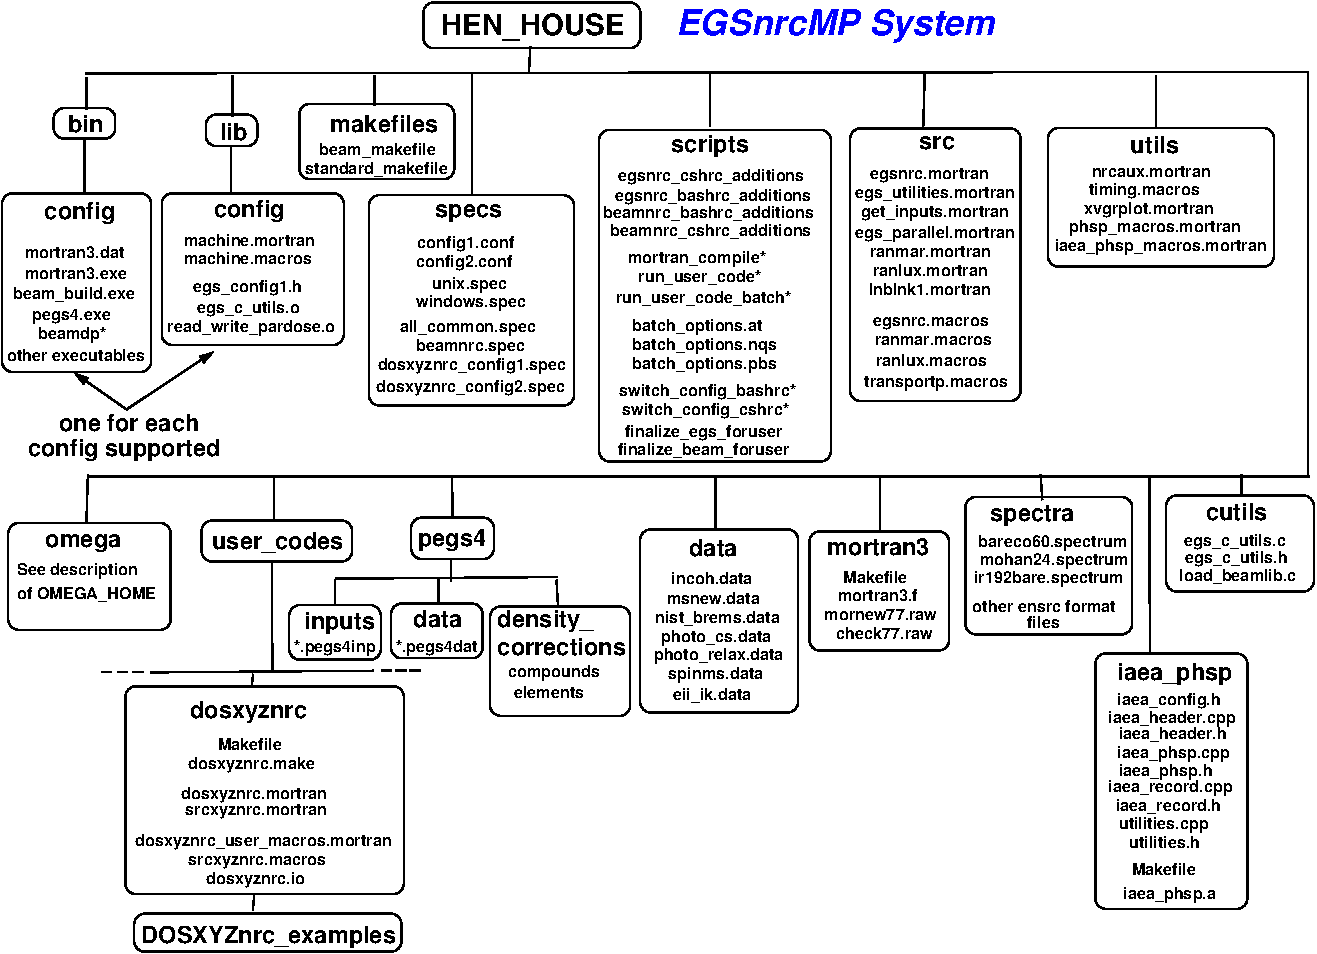
\includegraphics[width=15cm]{figures/egsnrc_system}
    \caption[Components of the {\tt HEN\_HOUSE} area for the EGSnrc
system.]
{The components of the {\tt HEN\_HOUSE} area for the EGSnrc
system. There are also subdirectories related to documentation and
NRC user codes which are not shown here and the main {\tt HEN\_HOUSE} box
actually has multiple subdirectories which are not shown. See PIRS-877 for
details\cite{Ka03}.}
\label{fig_hen_house_2}
\end{center}
\end{figure}

\clearpage

%\index{\$EGS\_HOME}
%\index{EGS\_HOME}
The second major  directory area of the EGSnrc system is
on the individual user's area and holds all the user's user codes and run associated
files.
It is mandatory that you set up a subdirectory which is referred to as
\verb+$EGS_HOME+ (e.g.,  frequently \verb+$HOME/egsnrc+) and for
each \verb+user_code.mortran+ which you use or write, there must be a sub-directory with
the same name as the user code, \ie~ \verb+$EGS_HOME/user_code+.
A typical user's area is shown in figure~\ref{fig_nrc_users_area}.
\begin{figure}[htb]
%\htmlimage{scale=1.6}   %this makes it readable
%\index{\$EGS\_HOME}
%\index{EGS\_HOME}
\index{EGSnrc!users area}
\index{user's area}
\begin{center}
\index{NRC EGSnrc user's area}
\index{user's area}
\leavevmode
\mbox{}\hspace{-1cm}
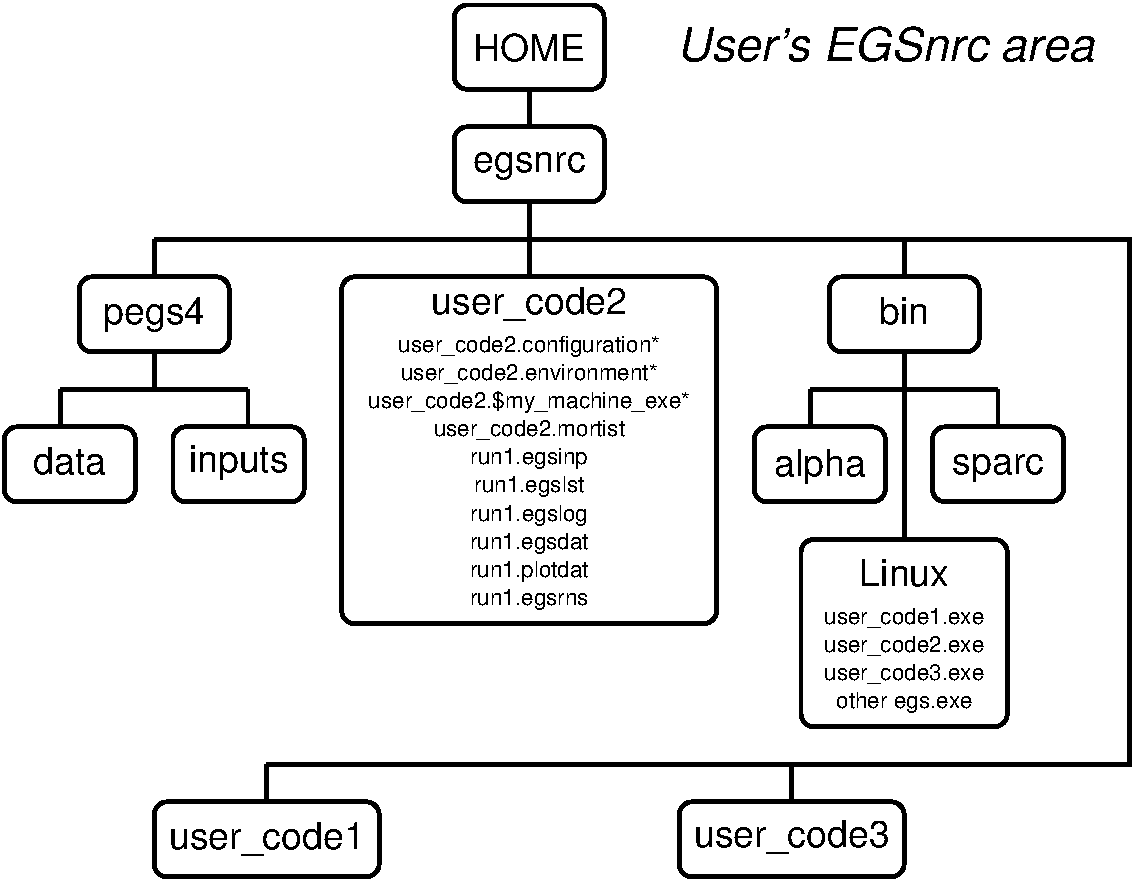
\includegraphics[width=14cm]{figures/users_egsnrc_area}
 \caption{Components of a typical EGS user's area where, for this
 example, {\tt \$EGS\_HOME} is {\tt \$HOME/egsnrc}. On a given system
 there can be an arbitrary number of different user's areas.
 \label{fig_nrc_users_area}
 }
\end{center}
\end{figure}

\subsubsection{A complication for multi-architecture systems}
\index{multi-architecture system}
% At NRC we run with a variety of different machines, all of which access
% a single disk system.  The EGSnrc system is set up to handle this
% transparently but this adds an additional level of complexity to the
% underlying system.  The system keeps track of which machine you are on
% at all times and uses the appropriate execute modules \etc.  This aspect
% of things is handled by the variable \verb+my_machine+ which essentially
% identifies the type of cpu currently being used and is determined by the
% script \verb+$HEN_HOUSE/get_machine+. The system is set up to store the
% executable files (the {\tt .exe}  files) on separate disk areas for each
% type of machine. To execute the code on different machine you must first
% compile it on each type of machine you want to use.  As new machines come
% along, the script \verb+$HEN_HOUSE/get_machine+ may become out of date and
% users may have to update it to return appropriate information for their
% system and more importantly, adjust the run and compile scripts to use the
% appropriate switches for their machine.
% \index{my\_machine}
% \index{get\_machine}
The install scripts are clever enough to establish various machine or
compiler dependencies and create the files {\tt
\$HEN\_HOUSE/lib/{my\_config}/machine.macros} and\\
 {\tt \$HEN\_HOUSE/lib/{my\_config}/machine.mortran} where {\tt
{my\_config}} is the name of your particular configuration (eg, g77,
gfortran, Mac).

\subsubsection{System aliases and environment variables}
\index{aliases} \index{environment variables}
\index{Cshrc\_additions\_for\_egsnrc}
\index{.login} \index{.cshrc}
\index{shell to use}
The EGSnrc system is based on using {\tt csh} C-shell scripts or {\tt sh},
bash shell scripts and to
facilitate this one should run from the C-shell ({\tt csh} or {\tt tcsh})
or the bash shell {\tt sh}.
To define the
aliases and other variables needed by the system, there are files called
{\tt egsnrc\_cshrc\_additions} and {\tt egsnrc\_bashrc\_additions} available on
{\tt \$HEN\_HOUSE/scripts}.
However, one first needs to set the environment variable {\tt HEN\_HOUSE}
to point at the location of the {\tt HEN\_HOUSE}. This is most conveniently
done with a declaration in your {\tt .login} file or {\tt .cshrc} file or
{\tt .bashrc} file depending on which shell is your default.
\begin{verbatim}
      setenv HEN_HOUSE location_of_HEN_HOUSE (e.g. $HOME/HEN_HOUSE)
\end{verbatim}
or for {\tt .bashrc}
\begin{verbatim}
      HEN_HOUSE=/absolute_location_of_your_HEN_HOUSE/ (e.g. $HOME/HEN_HOUSE)
\end{verbatim}
Then it is {\bfseries essential} that in your {\tt .cshrc} or {\tt .bashrc}
file you source the
{\tt  egsnrc\_cshrc\_additions} or {\tt egsnrc\_bashrc\_additions} file, i.e. add the statement:
\begin{verbatim}
     source $HEN_HOUSE/scripts/egsnrc_cshrc_additions}
\end{verbatim}
or, for those using {\tt bash}:
\begin{verbatim}
     source $HEN_HOUSE/scripts/egsnrc_bashrc_additions}
or
     source /absolute_location_of_your_HEN_HOUSE/scripts/egsnrc_bashrc_additions}
\end{verbatim}

These additions file set up many aliases and other variables for you. These
are most easily seen by executing the commands {\tt alias}, {\tt set} and
{\tt setenv} although this will show you all of the systems definitions as
well.  We will explain the use of many of these definitions in the
remainder of this section but the most important of the aliases are:
\index{egsnrc\_cshrc\_additions}
\index{egsnrc\_bashrc\_additions}

\index{mf} \index{mor} \index{f} \index{f} \index{ex} \index{mfb}
\index{PEGS4} \index{examin} \index{Mortran3!mor mf m}
\begin{description}
\item[mor]	MORTRAN a stand alone code
\item[m]	MORTRAN a specified users code
\item[mf]	MORTRAN and Fortran compile and link a specified users code
\item[f]	Fortran compile and link a specified users code
\item[ex]	execute an egs user code
\item[exb]	execute an egs user code in batch mode
%\item[pegs4]	run pegs4 (see section~\ref{pegs4_sc})
%\item[examin]   examin a particular data set from pegs4
%above not inlcuded now.
\end{description}
The use of these is described below in detail but note that the command
{\tt make} is now the easiest way to mortran and fortran user codes as
described in PIRS-877\cite{Ka03}.

% This script no longer here
%% The script {\tt
%% show\_settings} (on {\tt \$HEN\_HOUSE}) gives a more or less complete list
%% of all aliases, variables and environment variable associated
%% with EGSnrc once {\tt Cshrc\_additons\_for\_egsnrc} has been sourced. For
%% more detail see section~\ref{settings} (page~\pageref{settings}).
%% \index{show\_settings} \index{settings}



\newpage
\subsection{PEGS4}
\index{PEGS4}
\label{pegs4_sc}

As described elsewhere in this report, PEGS4 is the program which
prepares much of the material dependent cross section data sets required
by EGSnrc to do the simulations (see section~\ref{pegs4} on
page~\pageref{pegs4}).  As discussed there, use of the {\tt egs\_gui}
greatly facilitates the use of the {\tt PEGS4} program.

\index{.pegs4dat}
\index{.pegs4inp}
\index{densities for PEGS4}
The user must have the directories {\tt \$EGS\_HOME/pegs4},
{\tt \$EGS\_HOME/pegs4/inputs} and {\tt \$EGS\_HOME/pegs4/data}.
A user's PEGS4 input file is on {\tt \$EGS\_HOME/pegs4/inputs}
and has the name \verb+my_data.pegs4inp+.  The PEGS4 program outputs the
data file for EGSnrc to
\verb+$EGS_HOME/pegs4/data/my_data.pegs4dat+.
The listing file from the PEGS4
run is found on \verb+$EGS_HOME/pegs4+ and is called \verb+my_data.pegslst+.
To invoke PEGS4 one enters:
\begin{verbatim}
pegs4.exe -i inputfile [-o ofile] [-a] [-d density] [-x crosssection] [-e HEN_HOUSE]

inputfile.pegs4inp   the input file
output defaults to $HEN_HOUSE/pegs4/data/inputfile.pegs4dat
                or, if ofile is given, to $HEN_HOUSE/pegs4/data/ofile.pegs4dat
[-a]            => append results to output file
[-d density]    => use density.density   for density effect
[-x crosssection] => use $HEN_HOUSE/pegs4/crosssection instead of
                                $HEN_HOUSE/pegs4/pgs4pepr.dat
[-e HEN_HOUSE]  => use this absolute location as the HEN_HOUSE
\end{verbatim}
where \verb+my_data.pegsinp+ is the input file described in detail in
section~\ref{pegs4_input} (page~\pageref{pegs4_input}) and
\verb+density.density+
is a file containing the density effect information needed for this
particular calculation IF it is needed by \verb+my_data.pegsinp+.
The PEGS4 script checks the following directories, in order, for
the file \verb+density.density+.
\begin{verbatim}
$EGS_HOME/pegs4/inputs
$EGS_HOME/pegs4/density_corrections/elements
$EGS_HOME/pegs4/density_corrections/compounds
$EGS_HOME/pegs4/density_corrections
$HEN_HOUSE/pegs4/density_corrections/elements
$HEN_HOUSE/pegs4/density_corrections/compounds
\end{verbatim}

\subsubsection{Where pegs4 data is kept}
\index{PEGS4!where data is kept}
\index{.pegs4dat}
\label{wpdk}

Note that PEGS4 can only create one material output file per run and
if the simulation you want to run requires data for more than one material,
these must be joined into one \verb+file.pegs4dat+ file, either by
concatenation, by using an editor or by the {\tt -a} option in the command
line.

The EGSnrc run scripts look for the data file requested (see
section~\ref{Execution}), first on\\
\verb+$EGS_HOME/pegs4/data+ and if not
found there, then it looks on \verb+$HEN_HOUSE/pegs4/data+.
\vfill

\subsubsection{examin}
\index{EXAMIN}
The command:\\
\verb+examin -p file+
\\(note there is no ``e'' at the end of \verb+examin+) will allow you
to plot and/or list much of the photon and electron cross section data
in the file \verb+$EGS_HOME/pegs4/data/file.pegs4dat+ or if that is not
present, then in the file \verb+$HEN_HOUSE/pegs4/data/file.pegs4dat+. Note that
\verb+examin+ no longer displays the photon cross section data from the
PEGS4 data file but displays the data actually used by EGSnrc. The default
dataset used by \verb+examin+ is xcom. If you are using something else in your
user code, you must change the following line in the code:

\verb+REPLACE {$XDATA-DEFAULT} WITH {'xcom'}+

The output is found on \verb+$EGS_HOME/examin+. If requested, during execution
\verb+examin+ pops open \verb+xmgrace+ (a 2-D graphing package), otherwise
you have to use the listing files created. See section~\ref{examin}
(page ~\pageref{examin}).
\index{xmgrace}

\subsection{Compilation (MORTRAN and Fortran)}
\index{compiling}
\label{Compilation}

\index{Mortran3}

The EGSnrc system is written in the Mortran3 language which is
a pre-processor for Fortran.  Mortran3 is itself written in
Fortran.  The Mortran3 processor is part of the EGSnrc
distribution and is discussed in detail in section~\ref{UGM3},
page~\pageref{UGM3} of this report.  In order to create an executable file
from the mortran source files, there are two steps needed. The first step,
converts the mortran source code into standard Fortran77. We call this {\tt
MORTRAN} compiling.  The next step turns the Fortran source into an
executable, using the standard Fortran compile and link process.

Using the EGSnrcMP system (see PIRS-877\cite{Ka03}), the most direct way to
do these steps is using the {\tt make} command.  The following are the old
way to do it but they still work.

To ``compile'' the user code {\tt user\_code.mortran}, one issues the command:\\
\index{mf}\index{m}
\verb+mf user_code a [opt0|opt1|opt2|opt3|opt4]+\\
or\\
\verb+m user_code+\\

\index{Mortran3}
\index{Fortran}
The \verb+mf+ command will MORTRAN, Fortran and link the
entire user-code called \verb+user_code+, including the EGSnrc
system.  The Fortran and the execute modules are machine specific (SUN vs
SGI vs Linux etc) but this is handled in a transparent manner by the scripts.

The \verb+m+ command will MORTRAN the entire user-code
called \verb+user_code+, including the EGSnrc system. The output is
a Fortran file \verb+user_code_{my_machine}.f+ which is specific for the
machine being used since the script picks up a set of macros which
handles any differences between the machines.

The \verb+f+ command will Fortran and link the entire
Fortran version of the user-code called
\verb+user_code_{my_machine}.f+, which includes the EGSnrc system.
The scripts automatically detect the value for \verb+my_machine+ and use
the appropriate value.

\verb+user_code.mortran+ or \verb+user_code_{my_machine}.f+
must be present on area \\
\verb+$EGS_HOME/user_code+.

\index{compiling!options}
The letter {\tt a} after the user code name is a residual option which no
longer exists, but which has been left for compatibility with
a wide range of other scripts at NRC.  This option was associated with a
technique to avoid recompiling unchanged Fortran subroutines from one pass
to the next, but this was removed since compilers have become so fast that
it was not very useful and occasionally led to problems and always left
many extra files around. Note that  the
standard \verb+make+ facility does not work because the date on the Fortran
file is
always more recent than that on the object module since MORTRAN creates
a new version of the Fortran each time.


The option \verb+[opt0|opt1|opt2|opt3|opt4|debug]+ allows selection of
the optimisation level to be used.  For production codes, be sure to use
at least \verb+opt2+ since these can save up to 50\% over
\verb+opt0+, but they usually take much longer to compile and link.

\subsubsection{The  user\_code.configuration file (obsolete)}
\index{configuration file}
\index{.configuration file}
This approach has been completely revised and replaced by the {\tt
user\_code.make} file with {\tt SOURCES = } formats. See
PIRS-877\cite{Ka03}.  The same general capabilities have been maintained
in the new format.

During the MORTRAN stage, the scripts still create a file, called
\verb+.mortjob.mortran+ on \\
\verb+$EGS_HOME/user_code+. This file
contains all the source code for this
particular user\_code (macros, user\_code, and
any other routines the user wants, etc).
The files which are concatenated together to
form \verb+.mortjob.mortran+ are defined by the user.
% in the file\\
% \verb+$EGS_HOME/user_code/user_code.configuration+.  If this file is
% not present, the script uses the generic
% \verb+$HEN_HOUSE/standard.configuration+.  Figure~\ref{std_config} presents
% a listing of this file.
% \begin{latexonly}
% \input{standard.configuration}
% \end{latexonly}
% \begin{htmlonly}
% \clearpage
% \input{standard.configuration_html}
% \clearpage
% \end{htmlonly}



The {\tt .configuration} file (or new equivalent {\tt .make} file) allows for
very flexible options when compiling a given user
code.  For example, it is possible to change which random number generator
is being used throughout the system by merely changing which pair of files
are included in the configuration file, either {\tt ranlux.macros} and {\tt
ranlux.mortran} or {\tt ranmar.macros} and {\tt ranmar.mortran} (see
section~\ref{rngs}, page~\pageref{rngs}). However if
anything other than the default seeds and luxury levels are desired, there
may be some minor changes needed n {\tt user\_code.mortran}
unless one is very careful (\eg\ DOSRZnrc is designed to use either rng).
\index{RANMAR} \index{RANLUX}

\subsubsection{Order is Important}

The following still applies. When the file {\tt .mortjob.mortran} is
created, the order in which the various files are placed in the file is
important.  This is primarily because in Mortran3 the last definition of
any macro is the one that is in force.  Thus it is important that the {\tt
egsnrc.macros} file be read in early since this defines all of the default
values of the macros.  As long as it appears before the user code, then any
macro redefinitions done in the user code take precedence.

% the following no longer works so I removed the section
% \subsubsection{Batch compilations}
% \index{compiling!in batch}
% \index{batch!compiling}
% \index{batch}
% To compile in batch, just add a \verb+b+ to the above commands,
% \ie~\verb+mfb+ \etc. This will submit the compilation to whatever batch
% system you are using (see section~\ref{batch_que}).

\subsubsection{{\tt machine.mortran} files}
\index{machine.mortran}
Different compilers often have slightly different ways of handling certain
things.  The most common differences are regarding how files are opened
(i.e., the format of the {\tt OPEN} statement), and what is more difficult,
how they handle time.  EGSnrc itself has very few of these constructs
within it, but the user codes cannot avoid them.  To overcome these
differences, there are a series of macros defined in {\tt machine.mortran}
files which are found on {\tt
\$HEN\_HOUSE/lib/\$my\_machine/machine.mortran}.  It is even more complex
for Linux machines where the {\tt machine.mortran} files differ depending
on what version of the compiler you are using.  The default settings are
for a fairly recent {\tt g77} compiler but if you are using a slightly
older one you may need to edit the {\tt egs\_compile} script to select a
different default for the variable {\tt Linux\_compiler}.
\index{Linux\_compiler}

The {\tt  machine.mortran} files define a macro {\tt \$MACHINE} which the
user codes pick up. It is useful to define this properly in the {\tt
machine.mortran} which is picked up in your local environment.
\index{machine.mortran}
\index{\$MACHINE}

The above requirements are handled by a {\tt machine.mortran} which is
created for your system by the EGSnrcMP system as described in PIRS-877.


% no longer relevant so removed
% \subsubsection{{\tt get\_machine}, what if it fails?}
% \index{{get\_machine}}
% The script {\tt get\_machine} is designed to tell the EGSnrc scripts what
% type of machine is being used.  If the system you are using is not
% recognised by the scripts, it will try to compile using pretty vanilla
% flavoured compiler and loader flags.  The script will print out what flags
% it is using.  If you wish to change these to match the requirements of your
% machine, edit the {\tt egs\_compile} script. You may want to hard wire the
% selection of {\tt my\_flags} and {\tt my\_libs} to match your own
% machine/compiler.  If it is a common, new machine or compiler, please
% let us know what
% settings were needed and we will try to fit them into the next release.  We
% also hope to clean up these scripts and allow a more direct method to
% modify/tailor the system.
%



\subsection{Execution}
\index{execution}
\label{Execution}
\index{.egsinp}

The following works mostly still,, but there are new ways described in
PIRS-877\cite{Ka03} for the EGSnrcMP system.


Once a user code has been compiled, it is executed by issuing:

\hspace*{1cm}\verb+ex[b] user_code input data [queue|debug]+\vspace*{5mm}\\
\verb+$EGS_HOME/user_code/input.egsinp+ and\\
\verb+$EGS_HOME/user_code/user_code.{my_machine}_exe+ must exist.  The
PEGS4 data is in \verb+data.pegs4dat+ \index{.pegs4dat}which is located either on
the users area or the system area, as discussed in section~\ref{wpdk}.

\index{execution in batch}
If \verb+queue+ is not specified when the batch option ``{\tt b}'' is being
used, then the default queue on your system is used.
\index{interactive execution}

\index{debug}
In interactive mode, the 4-th input can be \verb+debug+ if a debug run
is wanted.  There must be an execute module created with the debug
switch set during compilation for this to work.

Execution of EGSnrc jobs is handled by the script {\tt egs\_run}
which is on the {\tt HEN\_HOUSE}.

At the completion of the run, all output and batch output files are
found on\\
\verb+$EGS_HOME/user_code/+ unless the user has specified something
different in the environment file (see below).

\index{execution!subdirectory during}
\index{subdirectory  during execution}
During execution, the {\tt egs\_run} script creates a separate subdirectory area
and only modifies the files there. This is usually a subdirectory of
\verb+$EGS_HOME/user_code/+ but on a Linux system is on {\tt /tmp}
(this is to
make the subdirectory local to the machine running the job since on the NRC
system, having the disk on another machine would seriously slow down the
job). All
the files are moved back to \verb+$EGS_HOME/user_code/+ after
completion of the run.  This can be confusing unless you are aware of this
behaviour.

\subsubsection{user\_code.environment file (obsolete)}
\index{.environment file}
\index{environment file}

This functionality is reworked and described in PIRS-877\cite{Ka03}.  In
particular the {\tt user\_code.io} file is relevant although the general
ideas below are still applicable.

% The execution scripts source
% \verb+$EGS_HOME/user_code/user_code.environment+ immediately prior to
% executing the \verb+user_code+ and then again immediately after.  An
% example  is given in
% \verb+$HEN_HOUSE/example_usercode.environment+ which is shown in
% figure~\ref{ex_environment}.  In general, this file defines the links to
% specific files from Fortran units, \etc.
%
Almost all Fortran compilers associate a file called {\tt fort.n} with any I/O
unit {\tt n} which is not attached explicitly within the code to some
file name. Thus if {\tt HATCH} read data from unit 12 without any open
statement, then it looks for {\tt fort.12}.  The system must associate
this file name to the real file name.
There are a series of similar links established
for files which have common names for all user codes.

% \begin{latexonly}
% \input{example_usercode.environment}
% \end{latexonly}
% \begin{htmlonly}
% \clearpage
% \input{example_usercode.environment_html}
% \clearpage
% \end{htmlonly}




The following files are associated with a normal type of run with an NRC
user code (although the environment files can add whatever files the user
may want and the files below are not mandatory).  For
this example, the input file name is \verb+input.egsinp+.
\begin{description}
\item [input.egsinp:] defined by the user.
\item [input.egslst:]  the output listing file from the run. Erased
at start of next run if not renamed.
\item [input.egslog:] The log file which echos the inputs and
prompts when running in batch. Note, this has most of the {\bf error}
messages too, so get in the habit of reading this file.
\item [input.egsdat:] A file containing all the information needed to
allow a calculation to be resumed.
\item [input.egsrns:] Some codes allow a record of random number seeds
at the start of each history to be kept (just most recent). These are
kept in this file if requested.
\item [input.egsplot (etc):] Plotting files for various routines, the
most up to date are for \verb+xmgrace+.
\index{xmgrace}
\item [input.egsgeom:] file with output description of geometry for
\verb+EGS_windows+.
\item [input.egsgph:] file with output phase space of each history for
\verb+EGS_windows+.
\end{description}

% The one known exception to the rule above about {\tt fort.n} files names is the
% HP unix system.  Here the default Fortran unit name is {\tt ftn05} for {\tt
% fort.5} etc. The approach here is to use statements like {\tt setenv ftn11
% fort.11} in the {\tt .environment} file prior to the link statement. This
% is done within {\tt egs\_run} for  many units which are regularly used.

\subsubsection{Batch Queues (obsolete)}
\label{batch_que}
See PIRS-877 for how this is handled now.


\subsection{Parallel Processing}
\label{pprocess}
\index{pprocess}
\index{parallel processing}
\index{NQS}

The following is replaced by a more sophisticated approach in the EGSnrcMP
system and the standard NRC user codes. See PIRS-877\cite{Ka03}.

Monte Carlo calculations with EGSnrc are easily run in parallel and the
results combined at the end of the runs because every history is completely
independent, as long as the random number sequences are independent. One of
the reasons for selecting the random number generators distributed with
EGSnrc is that there is a simple procedure for ensuring independent
sequences (see section~\ref{rngs} on page~\pageref{rngs}).

The NRC user codes\cite{Ro00} have a parallel processing option built in.
The system used requires the NQS batch submission system to be installed on
all machines to be run in parallel. The option is implemented via a script,
called {\tt pprocess} which makes an arbitrary number of input files from
the original file, ensuring different random number sequences for each and
then submitting the job to an arbitrary number of machines.  At the end of
the runs, the main user code is run once more with instructions to combine
the results of the previous runs.  Although crude, it is highly effective.
We routinely run using more than 30 of our 38 CPUs running in parallel.
The script {\tt combine\_egsnrc} has been written to automatically edit the
required input file and execute the needed final run for the analysis of
parallel runs with the NRC user codes.
There is more discussion in reference~\cite{Ro00}.
\index{combine\_egsnrc}

Note that there is a useful script called {\tt
clean\_after\_parallel} which is found on\newline {\tt \$HEN\_HOUSE/scripts}.
Parallel runs create a huge number of files and this script helps clean
them up, but only once they have been analysed.
\index{clean\_after\_parallel}


\subsection{Distribution / Installation of EGSnrc}
\label{install}
\index{distribution}
\index{installation}
\index{Cshrc\_additions\_for\_egsnrc}
\index{INSTALL\_EGS}


\index{.cshrc}
\index{HEN\_HOUSE}
This installation script requires that the environment variables
\verb+HEN_HOUSE+ not be defined when the script is called and not be
defined in the user's {\tt .cshrc} or {\tt .bashrc} file. The installation will create
the entire \verb+$HEN_HOUSE+ structure shown in
fig~\ref{fig_hen_house_2} (page~\pageref{fig_hen_house_2})
and compile a variety of codes for the machine
the user is doing the installation from (\viz\ Mortran3,
PEGS4, DOSRZnrc).  It also partially sets up the user's area
\verb+$EGS_HOME+.

Once the \verb+INSTALL_EGS+ script has been successfully executed, one
must ensure that the environment variables {\tt HEN\_HOUSE} and {\tt
EGS\_HOME} are defined to
point at wherever you have placed the EGSnrc system and your EGSnrc user
area.

Most importantly, the installation leaves behind a file called
\verb+egsnrc_cshrc_additions+ or \verb+egsnrc_bashrc_additions+
which MUST be sourced from the user's
{\tt .cshrc} script or {\tt .bashrc} script depending on which default
shell is used. Once the installation is complete,
add the following to your {\tt .cshrc} file:\\
\verb+source /explicit_path_to_your_HEN_HOUSE/egsnrc_cshrc_additions+. \\
or the following to your {\tt .bashrc} file:\\
\verb+source /explicit_path_to_your_HEN_HOUSE/egsnrc_bashrc_additions+. \\
\index{egsnrc\_bashrc\_additions}
\index{egsnrc\_cshrc\_additions}

The user should try to run the {\tt tutor} codes to ensure the system is working.

% For examples of the files created by {\tt INSTALL\_EGS}, see\\
% {\tt \$HEN\_HOUSE/test\_distribution\_outputs}.
% \index{example lst\_install files}
%
% One can also run the script {\tt test\_distribution} (see
% section~\ref{test_distribution}, page~\pageref{test_distribution}) which
% exercises the system extensively.
% \index{test\_distribution}.


% \subsection{On-Line Manuals}
% \index{on-line manuals}
% The manuals for the EGSnrc system are on-line from the same site as the
% distribution.
% \subsection{Changes and bugs corrected since initial release}
% \label{fixed_bugs}
% \index{bugs}
% \index{corrected bugs}
%
% %%%%%%%%%%%%%%%%%%%%%%%%%%%%%%%%%%%%%%%%%%%%%%%%%%%%%%%%%%%%%%%%%%%%%%%%%%%
% \noindent The following changes were made to EGSnrc in a minor release in Oct, 2001
% %%%%%%%%%%%%%%%%%%%%%%%%%%%%%%%%%%%%%%%%%%%%%%%%%%%%%%%%%%%%%%%%%%%%%%%%%%%
% \begin{itemize}
% \item A call to AUSGAB immediately prior to annihilation of a positron at
% rest was added with IARG=28.
%
% \item The auxiliary input routine for EGSnrc parameters was changed to use
% macros to define the defaults.
%
% \item A change was made to allow {\tt skindepth\_for\_bca} to be less than
% 1.
% \item James Tickner pointed out that K-alpha1 and K-alpha2 transition
% probabilities had been inverted.  This was fixed.
%
% \end{itemize}
%
% \noindent The following changes were made to EGSnrc in the May, 2001 release.
% \begin{itemize}
% \item WT = 0.0 now causes new particles to be discarded immediately via the
% \\
% {\tt USER-PHOTON-DISCARD} and {\tt USER-ELECTRON-DISCARD} exits which
% generate {\tt IARG = 3} exits.  This saves time and avoids other problems
% (see section~\ref{termination}, page~\pageref{termination}).
% \item {\tt \$COMIN-RELAX} is now defined in {\tt egsnrc.macros} instead of
% in {\tt subroutine relax}.
% \end{itemize}
%
% %%%%%%%%%%%%%%%%%%%%%%%%%%%%%%%%%%%%%%%%%%%%%%%%%%%%%%%%%%%%%%%%%%%%%%%%%%%
% \noindent The following bugs in EGSnrc were fixed in the May, 2002 release.
% %%%%%%%%%%%%%%%%%%%%%%%%%%%%%%%%%%%%%%%%%%%%%%%%%%%%%%%%%%%%%%%%%%%%%%%%%%%
%
% \begin{itemize}
% \item If using the SLAC geometry macros, the COMIN's did not contain the
% needed declarations of the variables.
% \item Daniel Frei from Bern pointed out an error which affected a charged
% particle going directly backwards along the Z axis.
% \item Format of the region number output by {\tt subroutine WATCH} was
% changed so that it would work for region numbers greater than 9,999. The
% original format caused {\tt EGS\_Windows} to misbehave.
% \item Alex Bielajew pointed out that egs\_batch does not work when using the
% standard at batch command due to extra white space.
% \item Permissions on data sets are changed to allow world read access.
% \item Omar Chibani pointed out that the density scaling didn't work
% properly. This has been fixed and the manual also made clearer.
% \item History by history statistical analysis was implemented in all user
% codes.
% \end{itemize}
%
% %%%%%%%%%%%%%%%%%%%%%%%%%%%%%%%%%%%%%%%%%%%%%%%%%%%%%%%%%%%%%%%%%%%%%%%%%%%
% \noindent The following bugs in EGSnrc were fixed in the Nov., 2003 release.
% %%%%%%%%%%%%%%%%%%%%%%%%%%%%%%%%%%%%%%%%%%%%%%%%%%%%%%%%%%%%%%%%%%%%%%%%%%%
%
%
% \begin{itemize}
% \item Many improvements to the GUI's and the entire new EGSnrcMP
% environment (see Report PIRS-877\cite{Ka03} for an extensive discussion).
%
% \item Fixed the ranlux RNG so that restarting a specific history is now
% possible (useful for debugging purposes).
%
% \item Fixed a bug pointed out by Rebecca Nutbrown re normalization of
% results when a phase-space source was recycled.
%
% \item Fixed a bug in FLURZnrc.mortran regarding electron fluence in bins
% below ECUT.
%
% \item Fixed a serious normalization bug in DOSRZnrc for the case where
% parallel runs were done using a phase-space source. The bug was pointed
% out by Roberto Capote who also pointed out a similar sort of bug which
% applied to all the RZ codes when using a phase space source and recycling
% the source.
%
% \item Bug in the {\tt preview3d} code for use with EGS\_Windows for
% cylindrical geometries was fixed.
%
% \item A bug, which was pointed out by Wamied Abdel-Rahman and Frank Verhaegen
% regarding positron annihilation when using the NIST cross sections for
% bremsstrahlung	production, was fixed.
%
% \item A bug related to discards for being below ECUT and PCUT in a vacuum
% was fixed.
% \end{itemize}
%
%
%
% \subsection{Known bugs/restrictions}
% \index{Known bugs}
% \index{restrictions}
%
% Straggling in the continuous energy loss is not modelled.
%






\clearpage
%%%%%%%%%%%%%%%%%%%%%%%%%%%%%%%%%%%%%%%%%%%%%%%%%%%%%%%%%%%%%%%%%%%%%%%%
\typeout{}
\typeout{***Start of Cited References****}
\typeout{}
%%%%%%%%%%%%%%%%%%%%%%%%%%%%%%%%%%%%%%%%%%%%%%%%%%%%%%%%%%%%%%%%%%%%%%%%
\renewcommand{\leftmark}{{References}}
\renewcommand{\rightmark}{{References}}

\section*{References}
\addcontentsline{toc}{section}{\numberline{}References}
\vspace*{-1.7cm}
\bibliography{../irs}
\typeout{}
\typeout{******REMEMBER to create .bbl  and reset twice**********}
\typeout{}
\bibliographystyle{unsrt}



\newpage
\typeout{**********starting index here******************}
\renewcommand{\leftmark}{{Index}}
\renewcommand{\rightmark}{{Index}}
\addcontentsline{toc}{section}{\numberline{}Index}
\setlength{\baselineskip}{0.5cm}


%%%%%%%%%%%%%%%%%%%%%%%%%%%%%%%%%%%%%%%%%%%%%%%%%%%%%%%%%%%%%%%%%%%%%%%%%%%%%%%
%
%  EGSnrc manual
%  Copyright (C) 2015 National Research Council Canada
%
%  This file is part of EGSnrc.
%
%  EGSnrc is free software: you can redistribute it and/or modify it under
%  the terms of the GNU Affero General Public License as published by the
%  Free Software Foundation, either version 3 of the License, or (at your
%  option) any later version.
%
%  EGSnrc is distributed in the hope that it will be useful, but WITHOUT ANY
%  WARRANTY; without even the implied warranty of MERCHANTABILITY or FITNESS
%  FOR A PARTICULAR PURPOSE.  See the GNU Affero General Public License for
%  more details.
%
%  You should have received a copy of the GNU Affero General Public License
%  along with EGSnrc. If not, see <http://www.gnu.org/licenses/>.
%
%%%%%%%%%%%%%%%%%%%%%%%%%%%%%%%%%%%%%%%%%%%%%%%%%%%%%%%%%%%%%%%%%%%%%%%%%%%%%%%
%
%  Authors:         Iwan Kawrakow
%                   Ernesto Mainegra-Hing
%                   Dave Rogers
%                   Frederic Tessier
%                   Blake Walters
%
%  Contributors:
%
%%%%%%%%%%%%%%%%%%%%%%%%%%%%%%%%%%%%%%%%%%%%%%%%%%%%%%%%%%%%%%%%%%%%%%%%%%%%%%%


\documentclass[12pt,twoside]{article}  %indexm doesn't work with two sides
%\usepackage{supertab}%this didn't work for some reason?

\usepackage{moreverb}	%this is used for the boxedverbatim environment
			%used to box the listing files for tutor programs
\usepackage{amsmath}
%\usepackage{showidx}    %shows index entries

\setlength{\textwidth}{16.51cm}
%\setlength{\textheight}{23.2cm}
\setlength{\textheight}{23.5cm}
\setlength{\oddsidemargin}{0.0in}
\setlength{\evensidemargin}{0.0in}
\setlength{\topmargin}{-1.5cm}
\setlength{\parindent}{1.5em}
\setlength{\topsep}{0ex}
\setlength{\itemsep}{0ex}

\newcommand{\Mol}{Moli\`ere}

\newcommand{\Co}{$^{60}$Co}
\newcommand{\parsp}{~\hspace*{1.5em}}
\setlength{\parskip}{0.1in}
\setlength{\baselineskip}{1.0cm}
\newcommand{\head}[1]{\begin{center}\begin{Large}{\bf #1}
                                              \end{Large}\end{center}}
\newcommand{\cen}[1]{\begin{center} #1 \end{center} }
\newcommand{\etal}{{\em et.al.}}
\newcommand{\ie}{{\em i.e.}}
\newcommand{\etc}{{\em etc.}}
\newcommand{\viz}{{\em viz.}}
\newcommand{\eg}{{\em eg.}}
\newcommand{\note}[1]{\mbox{}\\ \noindent \rule{16cm}{0.5mm} \\
{\em #1} \\ \noindent \rule{16cm}{0.5mm}\\
\typeout{***********note active on this page *************************}
}

%\newcommand{\indexm}[1]{\index{#1}}
%\typeout{~~~~~~~~~~~~***margin index feature OFF*****************************}
%\typeout{~~~~~~~~~~~~***margin index feature OFF*****************************}
%\typeout{~~~~~~~~~~~~***margin index feature OFF*****************************}
\newcommand{\indexm}[1]{\marginpar{{\sf {\tiny I:#1} }}\index{#1}}
\makeindex

%	some commands to get 4 levels in the table of contents and
%	number down to paragraphs
\setcounter{secnumdepth}{4}
\setcounter{tocdepth}{4}
\renewcommand{\thesubsubsection}{\thesubsection.\arabic{subsubsection}}
\renewcommand{\theparagraph}{\thesubsubsection.\roman{paragraph}}
\renewcommand{\theequation}{\arabic{subsection}.\arabic{subsubsection}.\arabic{equation}}

\renewcommand{\theenumii}{\roman{enumii}}
\renewcommand{\labelenumii}{\theenumii.}

%\renewcommand\paragraph{\@startsection{paragraph}{4}{\z@}%
%                                    {3.25ex \@plus1ex \@minus.2ex}%
%                                    {-1em}%
%                                    {\normalfont\normalsize\bfseries}}
%above is copied from article.cls and it still causes a hang up!!
%above explained p25-26 Latex Companion

\renewcommand{\refname}{}


\usepackage[breaklinks]{hyperref}
\usepackage{epsf}
\usepackage{graphicx}
\usepackage{epsfig}
\usepackage{longtable}

%\input{epsf}

%\usepackage{fancyheadings}
\usepackage{fancyhdr}
\usepackage{html}
\renewcommand{\footrulewidth}{0.4pt}
\renewcommand{\headrulewidth}{0.4pt}

\lhead[{\sffamily \thepage}]{{\sffamily {EGSnrc} Code System }}
\rhead[{\sffamily NRCC Report PIRS-701 }]{{\sffamily ~\thepage}}
%\rfoot[{\sffamily {\rightmark}}]{{\sffamily {\rightmark}}}
\rfoot[]{{\sffamily {\rightmark}}}
% Replace line with fixed date with the one below when commiting
% Beware: Using the macro below conflicts between CVS and latex!!!
% \lfoot[{\sffamily {\leftmark}}]{{\small Last edited $Date: 2013/09/26 17:59:57 $
\lfoot[{\sffamily {\leftmark}}]{{\small Last edited 2011/05/02 18:36:27
}}
\cfoot{}

\begin{latexonly}
\typeout{***Have turned off overfull and underfull messages****}
\tolerance=10000        %suppress Overfull only
\hbadness=10000         %suppress Overfull and Underfull for text (horizontal)
\vbadness=10000
\end{latexonly}

\begin{document}

\begin{htmlonly}
For information about the authors and/or institutions involved with this
work, use the links provided in the author list.\\
\begin{rawhtml}
<br><br>
\end{rawhtml}


\begin{rawhtml}
<br><br>
\end{rawhtml}

Postscript and pdf versions of the entire report are available.  You may have to
download the compressed version to disk, uncompress or gunzip them and
then read or print them.\\
\begin{center}
\htmladdnormallink{(uncompressed version 2.2 Mbyte)}{pirs701.ps}\\
\htmladdnormallink{(gzip version 670 kbyte)}{pirs701.ps.gz}\\
\htmladdnormallink{(pdf version 1.2 Mbyte)}{pirs701.pdf}
\end{center}
\begin{rawhtml}
<br><br>
\end{rawhtml}

Use the Up button to get back to this page from within the document.
\begin{rawhtml}
<BR> <HR> <P>
\end{rawhtml}
\copyright
Copyright 2000 -- 2015, National Research Council of Canada
Ottawa
\begin{rawhtml}
<BR> <HR> <P>
\end{rawhtml}
\end{htmlonly}

\pagestyle{empty}
%%%%%%%%%%%%%%%%%%%%%%%%%%%%%%%%%%%%%%%%%%%%%%%%%%%%%%%%%%%%%%%%%%%%%%%%

%               Title page to  preface

%%%%%%%%%%%%%%%%%%%%%%%%%%%%%%%%%%%%%%%%%%%%%%%%%%%%%%%%%%%%%%%%%%%%%%%%

\title{EGSnrc Code System}

\begin{center}
{\sffamily \bfseries {\Huge The EGSnrc Code System:}\\
{\Large Monte Carlo Simulation of Electron and Photon Transport
\vspace{5mm}\\}}
\begin{large}
I. Kawrakow\\
E. Mainegra-Hing, D.W.O. Rogers, F. Tessier and B.R.B. Walters\\
\end{large}
Ionizing Radiation Standards,\\
National Research Council Canada,\\
Ottawa, Canada\\

\vspace{10mm}
{\bfseries
\today}
\vspace{5mm}\\
\hfill NRCC Report {\sf PIRS-701} \vspace*{15mm}\\


\begin{figure}[h]
\begin{center}
\htmlimage{scale=1.2}
\leavevmode
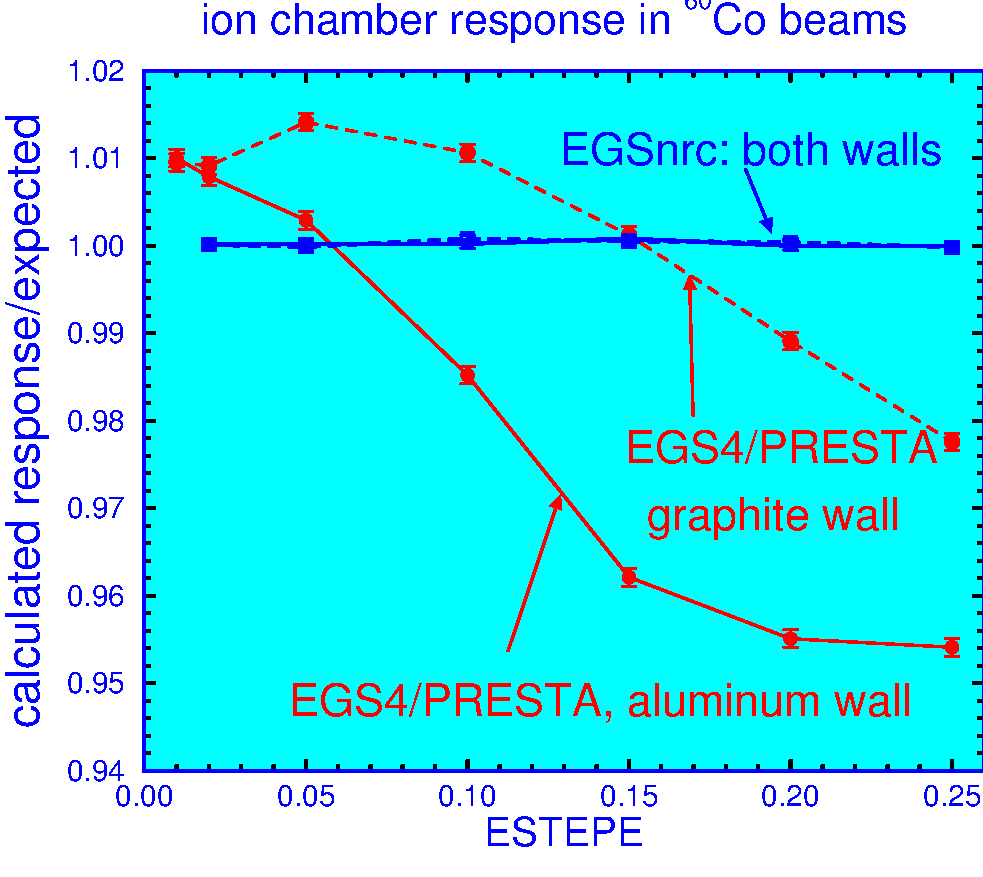
\includegraphics[height=10.5cm]{figures/ion_chamber}
%\caption{Improvement of EGSnrc compared to EGS4/PRESTA.}
%\cen{\Large Improvement of EGSnrc compared to EGS4/PRESTA.}
\end{center}
\end{figure}
\vfill

\copyright NRC Canada, 2001--2015
\end{center}
\newpage   %Blank page behind cover
\mbox{}


\newpage
\setlength{\baselineskip}{0.5cm}

\pagestyle{fancy}
\pagenumbering{arabic}
\setcounter{page}{1}


%%%%%%%%%%%%%%%%%%%%%%%%%%%%%%%%%%%%%%%%%%%%%%%%%%%%%%%%%%%%%%%%%%%%%%%%%%%%%%%
%
%  EGSnrc manual: preface
%  Copyright (C) 2015 National Research Council Canada
%
%  This file is part of EGSnrc.
%
%  EGSnrc is free software: you can redistribute it and/or modify it under
%  the terms of the GNU Affero General Public License as published by the
%  Free Software Foundation, either version 3 of the License, or (at your
%  option) any later version.
%
%  EGSnrc is distributed in the hope that it will be useful, but WITHOUT ANY
%  WARRANTY; without even the implied warranty of MERCHANTABILITY or FITNESS
%  FOR A PARTICULAR PURPOSE.  See the GNU Affero General Public License for
%  more details.
%
%  You should have received a copy of the GNU Affero General Public License
%  along with EGSnrc. If not, see <http://www.gnu.org/licenses/>.
%
%%%%%%%%%%%%%%%%%%%%%%%%%%%%%%%%%%%%%%%%%%%%%%%%%%%%%%%%%%%%%%%%%%%%%%%%%%%%%%%
%
%  Author:          Iwan Kawrakow, 2003
%
%  Contributors:    Blake Walters
%                   Frederic Tessier
%                   Ernesto Mainegra-Hing
%
%%%%%%%%%%%%%%%%%%%%%%%%%%%%%%%%%%%%%%%%%%%%%%%%%%%%%%%%%%%%%%%%%%%%%%%%%%%%%%%


\newpage
\mbox{ }\vspace*{-35mm}\\
\section*{\begin{center}Preface\end{center}}
\addcontentsline{toc}{section}{\numberline{}Preface}
\index{preface}
% Replace commented line for the one with fixed date when commiting
% Beware: Using the macro below conflicts between CVS and latex!!!
% \lfoot[{\sffamily {\leftmark}}]{{\small Last edited $Date: 2013/01/04 15:08:41 $
\lfoot[{\sffamily {\leftmark}}]{{\small Last edited 2011/05/02 18:36:27
}}
\mbox{ }\vspace*{-5mm}\\
\noindent {\bfseries Sixth printing: May 2011}\\
A long time has passed since the last update to this document.
Although no fundamental changes have been made to the system,
there have been a number of important additions and improvements
to the system since 2009. Numerous bugs have been corrected and
a new user code for free-air chamber (FAC) correction calculations
was added to the distribution.
\begin{itemize}
\item Use of arbitrary electron impact ionization (EII)
cross section compilations. Added a data base of EII
cross sections based on the DWBA/PWBA theory by
Bote and Salvat.
\item For backward compatibility with previous calculations, users can
now request the use of PEGS4 photon data.
\item Inclusion of C++ {\tt egs\_fac} application with example.
This user-code implements a self-consistent algorithm for the
fast calculation of FAC correction factors.
\item EII cross sections printout for materials in
  the simulation if user requests output of the photon cross-sections.
\item Updated several GUI's to include most of the latest additions
and corrected several bugs.
\end{itemize}
% \vspace{3mm}\\
\noindent {\bfseries Fifth printing: July 2009}\\
There has been a huge number of changes in the system since
the last printing in November 2003 that have not been properly
added to the documentation. This printing is an attempt to update
this report to better reflect the state of EGSnrc, although it
is far from complete. The development of the EGSnrc C++ class
library, which includes a general purpose geometry package, and its
first public release in 2005 has been a major step forward.
The C++ class library is described in a separate report (PIRS--898).
Major changes and additions to the EGSnrc physics include:
option to simulate electron impact ionization, an improved
bremsstrahlung data base that includes an exact evaluation of
electron-electron bremsstrahlung in the first Born approximation,
an improved differential pair production cross section tabulation
based on exact PWA calculations that takes into account the asymmetry
of the energy distribution at energies close to the threshold,
the ability to explicitely
simulate triplet interactions (\ie, pair production in the electron field),
the ability to take into account radiative corrections for Compton
scattering in the one-loop approximation, the ability to use
user-supplied atomic and molecular form factors for Rayleigh scattering,
and the ability to use total photon cross sections from EPDL97, XCOM, or
any other user-supplied tabulation in addition to the default
Storm \& Israel tabulations.
New options added for Compton scattering called {\tt simple} and
{\tt norej}. When using {\tt simple} binding is taken
into account via an incoherent scattering function
ignoring Doppler broadening. The incoherent scattering function
is still obtained from the impulse approximation.
The {\tt norej} option uses actual bound Compton cross section
when initializing the photon cross sections and rejections in
subroutine COMPT lead to re-sampling rather than rejecting the
entire interaction.
An {\tt alias sampling} algorithm is now used to select the
photon angle after a Rayleigh scattering to avoid an undersampling
at large angles observed in the original EGS4 implementation.
Particle track scoring object added to the {\tt egspp} library
allowing visualization of particle tracks with the C++ geometry
viewer {\tt egs\_view}. See example input file tracks1.egsinp for
the tutor7pp C++ user-code.

Finally, to better reflect their contributions
to the development and maintenence of the system, Ernesto Mainegra-Hing,
Blake Walters and Frederic Tessier have been added as co-authors.
\vspace{3mm}\\
\noindent {\bfseries Fourth printing: November 2003}\\
Added references to EGSnrcMP and Report PIRS-877. A few minor changes
related to the major change in the operating system to make it Windows
compliant. There is no associated change in the physics of the system.
Table 7 re timing of random numbers has changed substantially.
\vspace{3mm}\\
\noindent {\bfseries Third printing: April 2002}\\
Minor changes reflecting code changes.
%See section~\ref{fixed_bugs}.
\vspace{3mm}\\
\noindent {\bfseries Second printing: May 2001}\\
The second printing contains a description of the use of {\tt RHOF}
(section~\ref{RHOF_RHOR}, page~\pageref{RHOF_RHOR}) and {\tt \$SET-RHOF}
(section~\ref{set_rhof}, page~\pageref{set_rhof}). There is a brief new
discussion of {\tt combine\_egsnrc}, a script for automatic analysis of the
many files created by {\t pprocess} in parallel runs
((section~\ref{pprocess}, page~\pageref{pprocess})). There is a new section
about terminating histories with WT=0.0 (section~\ref{termination},
page~\pageref{termination}).
%Finally, a new section
%has been added which documents the few minor changes made to EGSnrc since
%its initial release ((section~\ref{fixed_bugs},
%page~\pageref{fixed_bugs})).
\vspace{3mm}\\
\noindent {\bfseries First printing: May 2000}\\
In the decade and a half since the original version of EGS4 was released
there have been well over 1000 papers published which cite the original
SLAC-265 Report.  The code itself has been improved in many different ways
by a large number of people.  For a detailed history of much of this up to
1994, the reader is referred to a report titled  ``History, overview and
recent improvements of EGS4'' by Bielajew et al.
\index{Bielajew, Alex}

In the last few years there have been significant advances in several
aspects of electron transport.  For example, improvements in multiple scattering
theory have been developed by Kawrakow and Bielajew\cite{KB97,Bi96,Ka96}
which get over most of
the shortcomings of the Moliere theory used in EGS4. Perhaps more important
has been the development by Kawrakow and Bielajew\cite{KB97a} of a new electron transport algorithm, sometimes
called PRESTA-II, which makes a significant advance in the science of
electron transport.  In addition to these advances, Kawrakow has implemented
several other improvements in the electron transport algorithm of EGS
which make it capable of accurately calculating ion chamber response at the
0.1\% level (relative to its own cross sections)\cite{Ka99a,Ka99b}.

EGSnrc also has implemented a variety of additional features, many of
which have previously been extensively developed as additions to EGS4
by  Namito, Hirayama and Ban at KEK as well\cite{Na98,Na95a,Na94,Na93}.
The EGSnrc approach differs from that of the KEK group, partially because
once we were making fundamental changes to the code, we carried it through
in a consistent manner. However, the KEK group have implemented several
options which are not yet in EGSnrc (e.g.  polarized photon scattering
and electron impact ionization).
\index{Hirayama, Hideo} \index{Namito} \index{Ban}

This report is meant to document the many changes that have occurred going
from EGS4 to EGSnrc.  Although this report is written by two people,
the EGS system is obviously the child of many parents who have made a
wide variety of contributions over the years.  This goes right back to
Richard Ford, then at SLAC, who was a major contributor to EGS3. Hideo
Hirayama, S Ban  and Yosh Namito of KEK have made innumerable contributions
to EGS, especially concerning the low energy photon physics. Alex
Bielajew worked on EGS at NRC from the early 80's to late 90's and his
name is linked to a huge number of important contributions to EGS,
perhaps most importantly the PRESTA algorithms, but also many other
specific improvements to the physics, the Unix based scripts and the NRC
user codes. His name appears very extensively in the reference lists.
The name of Walter Ralph Nelson is practically synonymous with EGS and
all users of any version of the EGS system will forever be in Ralph's
debt. It has been his enthusiasm and willingness to help others and share
this resource so selflessly which has made it the great success it is.
To all of these people who have contributed so extensively to the EGS
system, and to the countless others who have played a variety of roles,
we all owe a huge debt of gratitude.
\index{Nelson, Ralph}


It is worth noting that NRC and SLAC have drawn up a formal agreement which
recognizes that both have rights associated with EGS4 and EGSnrc.  Thus, in
this report there are sections which are taken verbatim from SLAC-265 (in
particular the PEGS4 manual and the User's guide to Mortran3) and we wish
to thank SLAC for permission to reproduce them.  We also draw attention to
the copyright and licensing arrangements associated with EGSnrc which are
similar to those for EGS4, but which are becoming more tightly controlled
in this changing world we live in.  Neither EGS4 nor EGSnrc are public
domain software. They are both copyright protected by NRC and/or SLAC. The
formal license statement is more precise and part of the package, but the
general meaning is that individuals are granted a without cost
license to use it for non-commercial purposes but that a license from NRC
is needed for any commercial application, and by definition someone working
for a for-profit organization or working on a contract for such an
organization is working on a commercial application.
\index{SLAC}


\noindent{\em What is next?\\}
In the section of the Preface to SLAC-265, there were 7 areas identified as
needing more work.  The work on EGS is not  complete, and at least 2 of
the 7 are still open, viz:
\begin{itemize}
\vspace{-4mm}
\item development of an efficient, general purpose geometry package
tailored to the EGS structure
\vspace{-3mm}
\item implementation of a general purpose energy loss straggling algorithm
which properly handles energy cutoffs
\end{itemize}

\vspace{-5mm}
There are other issues which are still undone within EGSnrc:
\vspace{-5mm}
\begin{itemize}
\item modeling of electron impact ionization
\vspace{-3mm}
\item some critical feature for your next application!!
\end{itemize}
We encourage users to contribute their improvements to the code. We will
happily add those which are of general interest and make available on the
distribution site those additions which are of special interest. We will
also appreciate receiving bug reports. Although we have done extensive QA
on the system, there have been many changes and not all parts of the code
are as carefully checked as we would like.  However, the pressure to release
the code is forcing us to proceed at this point.

We wish to thank our many colleagues at NRC who have helped with this work.
In particular Michel Proulx for his excellent help keeping the computer
systems going smoothly, Jan Seuntjens for his help with the user codes,
Joanne Treurniet for her help with the most recent version of the
EGS\_Windows system and Blake Walters for his work on QA of the system.

\noindent I.K and D.W.O.R.  \hfill Feb 2000 \vspace{1mm}\\

%\noindent {\bfseries Second printing: May 2001}\\
%The second printing contains a description of the use of {\tt RHOF}
%(section~\ref{RHOF_RHOR}, page~\pageref{RHOF_RHOR}) and {\tt \$SET-RHOF}
%(section~\ref{set_rhof}, page~\pageref{set_rhof}). There is a brief new
%discussion of {\tt combine\_egsnrc}, a script for automatic analysis of the
%many files created by {\t pprocess} in parallel runs
%((section~\ref{pprocess}, page~\pageref{pprocess})). There is a new section
%about terminating histories with WT=0.0 (section~\ref{termination},
%page~\pageref{termination}). Finally, a new section
%has been added which documents the few minor changes made to EGSnrc since
%its initial release ((section~\ref{fixed_bugs},
%page~\pageref{fixed_bugs})). \vspace{3mm}  \\
%\noindent {\bfseries Third printing: April 2002}\\
%Minor changes reflecting code changes. See section~\ref{fixed_bugs}.
%\vspace{3mm}\\
%\noindent {\bfseries Fourth printing: November 2003}\\
%Added references to EGSnrcMP and Report PIRS-877. A few minor changes
%related to the major change in the operating system to make it Windows
%compliant. There is no associated change in the physics of the system.
%Table 7 re timing of random numbers has changed substantially.
%\vspace{3mm}\\
%\noindent {\bfseries Fifth printing: July 2009}\\
%There has been a huge number of changes in the system since
%the last printing in November 2003 that have not been properly
%added to the documentation. This printing is an attempt to update
%this report to better reflect the state of EGSnrc, although it
%is far from complete. The development of the EGSnrc C++ class
%library, which includes a general purpose geometry package, and its
%first public release in 2005 has been a major step forward.
%The C++ class library is described in a separate report (PIRS--898).
%Major changes and additions to the EGSnrc physics include:
%option to simulate electron impact ionization, an improved
%bremsstrahlung data base that includes an exact evaluation of
%electron-electron bremsstrahlung in the first Born approximation,
%an improved differential pair production cross section tabulation
%based on exact PWA calculations that takes into account the asymmetry
%of the energy distribution at energies close to the threshold, the ability to explicitely
%simulate triplet interactions (\ie, pair production in the electron field),
%the ability to take into account radiative corrections for Compton
%scattering in the one-loop approximation, the ability to use
%user supplied atomic and molecular form factors for Rayleigh scattering,
%and the ability to use total photon cross sections from EPDL97, XCOM, or
%any other user-supplied tabulation in addition to the default
%Storm \& Israel tabulations. Finally, to better reflect their contributions
%to the development and maintenence of the system, Ernesto Mainegra-Hing,
%Blake Walters and Frederic Tessier have been added as co-authors.



\newpage

\tableofcontents

\newpage
\listoffigures
%\newpage
\listoftables

\setlength{\baselineskip}{0.5cm}

\newpage
%%%%%%%%%%%%%%%%%%%%%%%%%%%%%%%%%%%%%%%%%%%%%%%%%%%%%%%%%%%%%%%%%%%%%%%%

%		Introduction

%%%%%%%%%%%%%%%%%%%%%%%%%%%%%%%%%%%%%%%%%%%%%%%%%%%%%%%%%%%%%%%%%%%%%%%%

\renewcommand{\leftmark}{{1: Introduction}}
\typeout{Starting ``Introduction'' Should be on odd page}

%%%%%%%%%%%%%%%%%%%%%%%%%%%%%%%%%%%%%%%%%%%%%%%%%%%%%%%%%%%%%%%%%%%%%%%%%%%%%%%
%
%  EGSnrc manual: introduction
%  Copyright (C) 2015 National Research Council Canada
%
%  This file is part of EGSnrc.
%
%  EGSnrc is free software: you can redistribute it and/or modify it under
%  the terms of the GNU Affero General Public License as published by the
%  Free Software Foundation, either version 3 of the License, or (at your
%  option) any later version.
%
%  EGSnrc is distributed in the hope that it will be useful, but WITHOUT ANY
%  WARRANTY; without even the implied warranty of MERCHANTABILITY or FITNESS
%  FOR A PARTICULAR PURPOSE.  See the GNU Affero General Public License for
%  more details.
%
%  You should have received a copy of the GNU Affero General Public License
%  along with EGSnrc. If not, see <http://www.gnu.org/licenses/>.
%
%%%%%%%%%%%%%%%%%%%%%%%%%%%%%%%%%%%%%%%%%%%%%%%%%%%%%%%%%%%%%%%%%%%%%%%%%%%%%%%
%
%  Author:          Iwan Kawrakow, 2003
%
%  Contributors:    Blake Walters
%                   Frederic Tessier
%                   Ernesto Mainegra-Hing
%
%%%%%%%%%%%%%%%%%%%%%%%%%%%%%%%%%%%%%%%%%%%%%%%%%%%%%%%%%%%%%%%%%%%%%%%%%%%%%%%


\section{Introduction}
% Replace commented line for the one with fixed date when commiting
% Beware: Using the macro below conflicts between CVS and latex!!!
% \lfoot[{\sffamily {\leftmark}}]{{\small Last edited $Date: 2011/05/02 18:40:33 $
\lfoot[{\sffamily {\leftmark}}]{{\small Last edited 2011/05/02 18:36:27
}}
\subsection{Intent of this report}

\index{intent of report}
\index{purpose of report}
\index{acronym}
The EGS ({\bfseries E}lectron--{\bfseries G}amma--{\bfseries S}hower) system of computer codes is a general purpose package
for the Monte Carlo simulation of the coupled transport of electrons and
photons in an arbitrary geometry for particles with energies above a few
keV up to several hundreds of GeV.  This report introduces a new, enhanced version
called EGSnrc. In addition to explaining and documenting the various
enhancements and changes to the previous version (EGS4\cite{Ne85}),
this document includes several introductory and advanced tutorials
on the use of EGSnrc (section~\ref{tutorials}) and also contains
the \underline{EGSnrc Reference Manual}(section~\ref{ERM}),
the \underline{PEGS4 User Manual} (section~\ref{pegs4}), and
an \underline{EGS User Guide to Mortran3} (section~\ref{UGM3}).
Our intention has been to make this document wholly self-contained so
that the user need not refer to the original EGS4 User Manual\cite{Ne85}
although it is on-line and available at \htmladdnormallink{ {\sf
http://www.slac.stanford.edu/pubs/slacreports/slac-r-265.html}}
{http://www.slac.stanford.edu/pubs/slacreports/slac-r-265.html}.
The heart of the present report is Section 2 which documents the physics
in EGSnrc. This has changed substantially from the EGS4 comparable Chapter
2 because of the many changes in EGSnrc. However, we have chosen not to
repeat the general introduction to sampling and probability theory that
was in Chapter 2 of SLAC-265.

For a basic introduction to the code, see the reference manual,
section~\ref{ERM} (page~\pageref{ERM}).

\index{comparison to experiment}
We have not presented any comparisons with experiment in this
document since it has become such an extensive field that we have no
hope of reproducing a fraction of the data. Instead, we have prepared
a separate report on QA which presents extensive comparisons between
EGS4 and EGSnrc\cite{Wa00}. There are
significant differences in many situations because of the improved physics
in EGSnrc.  Two papers\cite{Ka99a,Ka99b} discuss many
of the details of the new physics, especially as related to ion chamber
calculations (which are perhaps the toughest test of any electron-photon
Monte Carlo transport code).  These papers provide analytic models which
explain many of the shortcomings of the EGS4/PRESTA system in this very
difficult problem.  The cover of this report shows a 
comparison of the two codes run in their standard default modes.
\index{ion chamber calculations}

\subsection{History of the EGS system}
\index{history}
\index{Bielajew, Alex}
The history has already been outlined in the Preface. For a detailed
history up to
1994, the reader is referred to a report titled  ``History, overview and
recent improvements of EGS4'' by Bielajew et al. That
report draws heavily on the history sections of the 
SLAC-210\cite{FN78} and SLAC-265\cite{Ne85} reports with an update to
1994.

As stated in the Preface, EGSnrc is the child of many parents who have
made a wide variety of contributions over the years. We will not repeat
the preface here except to note that Walter ``Ralph'' Nelson has been
the key player in the development of the system over the years and we
all owe him a debt of gratitude.
\index{Nelson, Ralph}


\subsection{Summary of EGSnrc Capabilities and Features}
\index{EGSnrc!summary capabilities}
\index{capabilities of EGSnrc}
\index{EGSnrc!features}
\index{features of EGSnrc}

The following is a summary of the main features of the EGSnrc
Code System, including statements about the physics that
has been put into it and what can be realistically simulated.

\begin{itemize} 
\item The radiation transport of electrons ($+$ or $-$) or photons
can be simulated in any element, compound, or mixture.  
The data preparation package, PEGS4, creates data to be used by
EGSnrc, using cross section tables for elements 1 through 100. In addition
there are other data files which must be read in to implement many of the
new options.

\item Both photons and charged particles are transported in
steps of random length rather than in discrete steps.

\index{low energy limit!electron}
\index{low energy limit!photon}
\item The dynamic range of charged particle kinetic energies
goes from a few tens of keV up to a few hundred GeV.  Conceivably
the upper limit can be extended higher, but the validity of the
physics remains to be checked.

\index{allowed energy range}
\index{energy range}
\item The dynamic range of photon energies lies between 1 keV and
several hundred GeV (see above statement).

\item The following physics processes are taken into account
by the EGSnrc Code System:

\index{physics processes in EGSnrc}
\index{EGSnrc!physics processes}
\begin{itemize} 
  \item Bremsstrahlung production using either Bethe-Heitler cross sections
or the NIST cross sections.

  \item Positron annihilation in flight and at rest
  (the annihilation quanta are followed to completion).

  \item Multiple scattering of charged particles by coulomb scattering from
nuclei is handled using a new
multiple scattering theory which overcomes the shortcomings of Moli\`ere 
multiple scattering theory. It allows for steps of any size and
moves seamlessly from a single scattering
model for short steps to an  accurate multiple scattering model
at large steps.  The user has the option of scattering based on
Rutherford scattering or scattering accounting for relativistic and spin
effects.

  \item M\o ller ($e^-e^-$) and Bhabha ($e^+e^-$) scattering.
  Exact rather than asymptotic formulae are used.

  \item Continuous energy loss applied to charged particle
  tracks between discrete interactions.
    \begin{itemize} 
    \item Total restricted charged particle stopping power consists of 
    soft bremsstrahlung and collision loss terms.
     
    \item Collision loss determined by the restricted
    Bethe-Bloch stopping power with Sternheimer treatment of
    the density effect in the general case but with provision of using
    an arbitrary density effect correction and data supplied to use the
    density effect recommended by the ICRU in Report 37.
    \end{itemize} 

  \item Pair production.
   
  \item Compton scattering, either Klein-Nishina or bound Compton.
   
  \item Coherent (Rayleigh) scattering can be included
  by means of an option.
   
  \item Photoelectric effect.
    
  \item Relaxation of excited atoms after vacancies are created (eg after
      photoelectric or Compton scattering events) to create fluorescent photons 
     (K, L, M shells) and Auger and Coster-Kronig
     electrons may be produced and tracked if requested.

  \item Electron impact ionization can be modeled using arbitrary theories
        for generating cross-sections. Five such cross-section compilations 
        are provided in the EGSnrc distribution (Kawrakow, Casnati, 
        Kolbenstvedt, Gryzinski, and Bote and Salvat).

\end{itemize} 
 
\item PEGS4 is a stand-alone data preprocessing code consisting of
12 subroutines and 85 functions.  The output is in a
form for direct use by EGS4.
\begin{itemize} 
   
  \item PEGS4 constructs piecewise-linear fits over a large
  number of energy intervals of the cross section and branching
  ratio data.
   
  \item In general, the user need only use PEGS4 {\it once} to
  obtain the media data files required by EGSnrc.
   
  \item PEGS4 control input uses the NAMELIST read facility of
  the FORTRAN language (in Mortran3 form).
   
  \item In addition to the options needed to produce data for
  EGSnrc, PEGS4 contains options to plot any of the physical
  quantities used by EGSnrc.
 
  \item In addition to the material specific data files produced by PEGS4,
   EGSnrc uses a variety of other data files as input for the calculations.
\end{itemize} 
 
\item EGSnrc is a package of subroutines plus block data with
a flexible user interface.
   
  \begin{itemize} 
  \item This allows for greater flexibility without requiring
  one to be overly familiar with the internal details of the code.
   
  \item Together with the macro facility capabilities of the
  Mortran3 language, this reduces the likelihood that user edits
  will introduce bugs into the code.
   
  \item EGSnrc uses material cross section and branching ratio
  data created and fit by the companion code, PEGS4. However,
  photon cross-section data are re-calculated on-the-fly
  using a logarithmic energy grid with an user-specific number
  of interpolation points. This behaviour can now be reverted
  if the user so desires.
 
\index{EGSnrc!geometry}
\item The geometry for any given problem is specified by a
{\it user-written} subroutine called HOWFAR which, in turn,
can make use of auxiliary subprograms.
   
  \item Auxiliary geometry routines for planes, cylinders,
  cones, spheres, etc., are provided with the EGSnrc Code System
  for those who do not wish to write their own.
   
  \item Macro versions of these routines are also provided in the
  set of defining macros (\ie, in the {\tt egsnrc.macros} file) which,
  if used, generally result in a faster running simulation.
   
   
\index{magnetic field transport}
\index{electric field transport}
  \item Transport can take place in a magnetic field by writing
  a specially designed HOWFAR subprogram, or in a more general
  manner (\eg, including electric field) by making use of
  Mortran3 macro templates that have been appropriately placed
  for that purpose in subroutine ELECTR.The file {\tt emf\_macros.mortran}
  contains Bielajew's macros to implement this.
   \index{emf\_macros.mortran}
   \index{Bielajew, Alex}
  \end{itemize} 
 
\item The user scores and outputs information in the
{\it user-written} subroutine called AUSGAB.
   
  \begin{itemize} 

  \item By setting various {\tt AUSFLG} flags, the user can arrange to have
access to the simulation parameters under many different situations to
allow scoring of almost any parameter of interest with out delving into the
code itself.

  \item Auxiliary subprogram WATCH is provided in order to allow
  an event-by-event or step-by-step tracking of the simulation, either to
the terminal or for 3-D graphics display using the program EGS\_Windows.
 \end{itemize} 
 
\item EGSnrc allows for the implementation of {\it importance
sampling} and other variance reduction techniques (\eg, leading
particle biasing, splitting, path length biasing, Russian
roulette, etc.). 
  \begin{itemize} 
  \item EGSnrc introduces options to allow for efficient bremsstrahlung 
    splitting and Russian Roulette of secondary charged-particles, but only 
    if ``turned on'' by the user.
  \item EGSnrc calculates the range and distance of the particle to the
   nearest boundary on every step as part of the electron transport algorithm
   and there is an option to do range rejection on any particle that cannot get out of
   the current region.
 
\end{itemize} 

\item Initiation of the radiation transport:
   
\begin{itemize} 
  \item An option exists for initiating a shower with two
  photons from pi-zero decay (\ie, use $IQI=2$ in the
  {\tt CALL SHOWER} statement). 
   
  \item The user has the choice of initiating the transport
  by means of a monoenergetic particle, or by sampling from
  a known distribution (\eg, a synchrotron radiation spectrum).
   
  \item Transport can also be initiated from sources that have
  spatial and/or angular distributions.

  \end{itemize} 
\end{itemize} 


\newpage
\subsection{Summary of changes from EGS4}
\label{changes_summary}
\index{changes from EGS4}
\index{EGS4}
\index{EGS4!changes from}
This is a brief listing of these changes which are discussed more fully in
section~\ref{section_2} and in section~\ref{changes}.

\subsubsection{Physics changes}

\begin{itemize} 
\item A completely new electron transport algorithm is used which removes
all known shortcomings of the EGS4/PRESTA algorithm.  If the geometry
permits, the new algorithm can take much larger steps with better accuracy
than previously. As it crosses a boundary, it goes into single scattering
mode to ensure an accurate boundary crossing. The EGS4/PRESTA algorithm
is still available as an option.

\item A new multiple scattering theory is used which gets around the
shortcomings of Moliere multiple scattering theory. It seamlessly goes from
a single scattering mode for short steps to a multiple scatter mode for
long steps.

\item Within the new multiple scattering theory an option has been added to
include relativistic spin effects in the cross section instead of just the
Rutherford cross section which underlies Moliere theory.

\item If desired, it is possible to do the entire calculation modeling
elastic scattering in a single scattering mode. This is at the cost of a
great deal of computing time and also does not model the inelastic energy
losses in a single scattering model.

\item A relaxation simulation feature has been added which allows creation
and following of fluorescent photons from K, L, M shells, Auger electrons and
Coster-Kronig electrons. Currently this can be called after photo-electric
and Compton scattering events.

\item If relaxation is not being modeled, then a photo-electron in EGSnrc
carries the entire energy of the incident photon. This is a better
approximation in most cases than dumping the binding energy locally and
subtracting the binding energy from the photo-electron's energy (as done in
EGS4).

\item Sampling the angular distribution of the photo-electron is available
as an option.

\item Bound Compton scattering can be simulated as well as Klein-Nishina
Compton scattering.

\item Bremsstrahlung angular sampling has been changed from a fixed angle
approximation to allowing the angular distribution to be sampled in one of
two ways.

\item A bug was fixed in the bremsstrahlung photon energy sampling routine
which affected simulations for which AP was not small relative to the electron
energy.  Doing this led to a complete rewrite of the sampling routine which
also increased its efficiency.

\item A second bremsstrahlung photon energy sampling option was added which 
uses the more accurate NIST differential cross sections.

\item PEGS4 has been modified to pick up the data files which scale the
radiative cross sections to produce the NIST/ICRU 37 radiative stopping
powers.

\item A variety of variance reduction techniques which were commonly used
with EGS4 have been ``built in'' with EGSnrc to improve the efficiency
   \begin{itemize} 
   \item bremsstrahlung splitting is done within the routine BREMS, thereby
         avoiding repeatedly calculating several constants
   \item Russian Roulette of secondary charged particles is done in a
         manner which sometimes avoids sampling the particles phase space unless
         it survives.
   \item range rejection, viz the termination of a particle history, when
         it cannot escape the local region, is implemented naturally and
         very efficiently since the particle range and distance to the
	 nearest boundary are already calculated on every step.
   \end{itemize}

\item Subroutine HATCH has been modified considerably to allow
initialization for the many new options.

\item The Moller sampling routine was corrected as first done in the
1997 release of EGS4.


\item The efficiency of the annihilation sampling routine has been
improved.

\item The sampling of the azimuthal angle has been recoded and saves a
noticeable amount of time in a real calculation (2\% in one example).

\item Various changes have been made in the COMIN blocks to accommodate the
above changes. Also LATCH and LATCHI are  now a default part of STACK. 

\item Several more AUSGAB calls are available to score Auger
and Coster-Kronig electrons and fluorescent x-rays.

\end{itemize} 



\subsubsection[System changes]{System changes pre-EGSnrcMP(see
ref\cite{Ka03} for the MP changes)}
\index{EGSnrc!system changes}
\begin{itemize} 

\item The various source files have been rationalized and various add-on
features to EGS4 have been made part of EGSnrc.

\index{ranmar} \index{ranlux} \index{parallel processing}
\item Two options for random number generator are available. The
default is the RANLUX generator which allows various ``luxury levels''
of generator to be used and the RANMAR generator, which had become the
standard for the Unix distribution of EGS4, is also available, although
re-coded.  Both generators have the ability to generate sequences which
are known to be independent and thus can be used for parallel processing.
At the default luxury level of 1, the RANLUX generator is slightly slower
than the recoded RANMAR generator, but the difference has a negligible
impact on overall computing time.

\item The default for calculating sines is now a function call because
modern machines do this very rapidly and the table lookup method is known
to be inaccurate for very small angles.

\item The EGS\_Windows code for generating  3-D interactive displays has
been ported to run on any X-windows platform using non-proprietary
software.

\item The entire code has been written using {\tt IMPLICIT NONE}. Further,
all declarations have been done using {\tt \$REAL} and {\tt \$INTEGER}
constructs which allow conversion to running double precision by redefining
2 macros, as long as the user codes  do the same thing!

\item Subroutine WATCH has been modified to accommodate the changes in the
physics.

\end{itemize} 

\subsubsection{User code changes}
\index{User codes}

\begin{itemize} 
\item The tutor codes have been rewritten to work with EGSnrc and a new
version of tutor6 has been written to demonstrate control of all variables
available to EGSnrc users.

\item Four of the standard NRC user codes for cylindrical geometry problems
 are now distributed with the system, DOSRZnrc, FLURZnrc, CAVRZnrc and
SPRRZnrc.

\item The above user codes have been extensively reworked to use a
new generalized input package which makes it much easier for the user
to generate the input files since the inputs are text oriented. Also,
the geometry and physics transport inputs are common for all codes.

\item The output routines have been reworked to avoid the use of
VAX extensions to Fortran which were not available with many Unix compilers.

\item The user codes have been cleaned up to some extent although not as
much as desirable! The main user codes systematically use {\tt
\$IMPLICIT-NONE}
and {\tt \$REAL, \$INTEGER} constructs to allow compatibility with EGSnrc and
the ability to change to double precision at will.

\item a bug in the energy sampling routine which caused problems in some
cases has been removed. An entirely new code which is faster and more
accurate is used now.
\end{itemize} 

\subsection{Summary of changes since 2005 edition of this report}

\subsubsection{Physics changes since 2005} 

\begin{itemize}

  \item Electron impact ionization can be modeled using four different theories
        for generating cross-sections (Kawrakow, Casnati, Kolbenstvedt, or
        Gryzinski).

  \item The user has the option of supplying custom molecular form factors
        when including Rayleigh scattering in a simulation.

  \item New {\tt alias sampling} algorithm used to select the 
        photon angle after a Rayleigh scattering.

  \item New options added for Compton scattering called {\tt simple} and 
        {\tt norej}.

  \item The user has the option to include radiative corrections for Compton
        scattering.

  \item The user has the option to use exact PWA cross sections for pair 
        production

  \item The user has the option to explicitely simulate triplet production

  \item A new bremsstrahlung data base has been added that incorporates a much 
        improved evaluation of electron-electron bremsstrahlung

  \item The ability to use total photon cross sections from EPDL-97, XCOM, 
        or any other user-supplied tabulation has been added


\end{itemize}

\subsubsection{ EGSnrc snapshots }

Since 2008 development snapshots of the EGSnrc system have been made 
available on the EGSnrc web page. These snapshots are updated much more 
regularly (typically every 2--8 weeks) but for now they can only be installed 
via a significantly simplified script on Linux systems with the GNU compilers. 

\subsubsection{User code changes since 2005}

\begin{itemize}

\item Two tutor codes, {\tt tutor2pp} and {\tt tutor7pp}, have been
added which make use of the C++ class library.  These codes are the
C++ equivalents to {\tt tutor2} and {\tt tutor7}.

\item Four new user codes which use the EGSnrc C++ class library have
also been added: 1) {\tt egs\_cbct} for simulating cone beam CT scans,
2) {\tt egs\_chamber} for efficient chamber simulations, 3) {\tt egs\_fac}
for simulating transport in a free-air chamber, and 4) {\tt egs\_pet} for
simulating PET scans, in addition to {\tt cavity}, the first major C++ code 
for EGSnrc released in 2005. Note that {\tt egs\_cbct} and {\tt egs\_pet} 
are not included in this public release.

\end{itemize} 

\subsection{Summary of changes since 2009 edition of this report}

There have been several additions to the physics 
and to the user codes available since the 
2009 edition of PIRS-701.  These are outlined in this section.

\subsubsection{Physics changes since 2009} 

\begin{itemize}

  \item A new electron impact ionization (EII) cross-section data base, 
        based on the DWBA/PWBA model by Bote and Salvat has been added
        to the distribution.

  \item The ability to use different EII cross section compilations
        has been generalized to allow the use of any user-supplied 
        tabulation.

  \item The user has the option of forcing the use of photon 
        cross-sections from the PEGS4 data file.

\end{itemize}

\subsubsection{ EGSnrc snapshots }

Since 2010 no snapshots of the EGSnrc system have been made 
available on the EGSnrc web page. The number of users making use
of this option is so small that it doesn't justify the effort put 
into creating them.

\subsubsection{User code changes since 2009}

The C++ user-code {\tt egs\_fac} has been finally included in the
distribution. This user-code simulates the transport in a 
free-air chamber and the calculations of correction factors
in a self-consistent manner. The user-codes {\tt egs\_cbct} 
and {\tt egs\_pet} are not included since they are in a very
experimental stage and not ready for public release.

\subsection{Outline of report}

In the remainder of this report there are 7 sections.  

Section 2 (page~\pageref{section_2}) presents a detailed description
of the physics in EGSnrc. While this section provides very important
documentation of what the code is doing, it is not essential reading in
order to get the code working.  Arguably it is essential reading before
you can use the code really well!

Section 3 (page~\pageref{ERM}) provides a detailed reference manual
which tells you what must be done to write your own user code.

Section 4 (page~\pageref{tutorials}) presents a series of short tutorial
programs which demonstrate the essential elements of EGSnrc user codes.
These are designed for those who learn by seeing examples (like DWOR).

Section 5 (page~\pageref{changes}) presents a summary of the changes
compared to EGS4 and a step by step procedure for upgrading an EGS4 user
code to work with EGSnrc.

Section 6 (page~\pageref{pegs4}) is the PEGS4 Users manual taken directly
from SLAC-265 along with a few additional pieces of documentation,
mostly about the upgrades since the original PEGS4 was released.

Section 7 (page~\pageref{UGM3}) is an EGS user guide to Mortran3, again
taken directly from SLAC-265.

Section 8 (page~\pageref{sys_consid}) outlines various system
considerations associated with running EGSnrc in a Unix environment. It
also discusses installation and distribution of the code.

We also draw your attention to the index which may help  find things.


\subsection{Associated documents}

%%%%%%%%%%%%%%%%%%%%%%%%%%%%%%%%%%%%%%%%%%%%%%%%%%%%%%%%%%%%%%%%%%%%%%%%%%%%%%%
%
%  EGSnrc manual: associated documents
%  Copyright (C) 2015 National Research Council Canada
%
%  This file is part of EGSnrc.
%
%  EGSnrc is free software: you can redistribute it and/or modify it under
%  the terms of the GNU Affero General Public License as published by the
%  Free Software Foundation, either version 3 of the License, or (at your
%  option) any later version.
%
%  EGSnrc is distributed in the hope that it will be useful, but WITHOUT ANY
%  WARRANTY; without even the implied warranty of MERCHANTABILITY or FITNESS
%  FOR A PARTICULAR PURPOSE.  See the GNU Affero General Public License for
%  more details.
%
%  You should have received a copy of the GNU Affero General Public License
%  along with EGSnrc. If not, see <http://www.gnu.org/licenses/>.
%
%%%%%%%%%%%%%%%%%%%%%%%%%%%%%%%%%%%%%%%%%%%%%%%%%%%%%%%%%%%%%%%%%%%%%%%%%%%%%%%
%
%  Author:          Iwan Kawrakow, 2003
%
%  Contributors:    Blake Walters
%                   Frederic Tessier
%                   Ernesto Mainegra-Hing
%
%%%%%%%%%%%%%%%%%%%%%%%%%%%%%%%%%%%%%%%%%%%%%%%%%%%%%%%%%%%%%%%%%%%%%%%%%%%%%%%

% Replace commented line for the one with fixed date when commiting
% Beware: Using the macro below conflicts between CVS and latex!!!
% \lfoot[{\sffamily {\leftmark}}]{{\small Last edited $Date: 2011/05/02 18:36:27 $
\lfoot[{\sffamily {\leftmark}}]{{\small Last edited 2011/05/02 18:30:41
}}

\index{associated documents}
There are a variety of papers which have been written about EGSnrc and
several NRC reports which are part of the distribution.  These are
listed below.  There are also a large number of papers which have been
written about EGS4.

\subsubsection{Refereed Papers}
\begin{itemize}
\item {\bfseries Accurate condensed history Monte Carlo simulation of
     electron transport. I. EGSnrc, the new EGS4 version:} \\
 I. Kawrakow, Medical Physics, {\bf 27} (2000) 485 -- 498.\\
Describes the overall implementation of the new electron transport
physics in EGSnrc.

\item {\bfseries Accurate condensed history Monte Carlo simulation of
     electron transport. II. Application to ion chamber response
     simulations:}\\
 I. Kawrakow, Medical Physics, {\bf 27} (2000) 499 -- 513.\\
Quantifies which problems in EGS4 led to the difficulties simulating ion
chamber response accurately and demonstrates that EGSnrc does not have
these problems.

\item {\bfseries Monte Carlo study of Spencer-Attix cavity theory at low
     photon energies:}\\
J. Borg, I. Kawrakow, D.W.O. Rogers and J.P.  Seuntjens, Med. Phys. {\bf
 27} (2000) 1804 -- 1813.
\\Uses code to explore the accuracy of Spencer-Attix cavity theory.
Paper demonstrates the accuracy of the EGSnrc code system for calculations
related to real ion chambers.


\item {\bfseries On the representation of electron multiple
elastic-scattering distributions for Monte Carlo calculations:}\\
I. Kawrakow and A. F.  Bielajew, Nucl. Inst. Meth. B 134, (1998) 325 --
336\\ Describes the multiple scattering theory used in EGSnrc.

\index{Bielajew, Alex}
\item {\bfseries On the condensed history technique for electron
transport:}\\
I. Kawrakow and A. F.  Bielajew, Nuclear Instruments and
Methods B 142 (1998) 253 -- 280.\\ Describes the electron transport
algorithm used in EGSnrc and demonstrates its improved accuracy compared
to all other published algorithms.


\end{itemize}
\subsubsection{Internal Reports}
\begin{itemize}
\item {\bfseries Monte Carlo calculated wall and axial non-uniformity
     corrections for primary standards of air kerma},\\
D. W. O.  Rogers and J. Treurniet, NRC Report PIRS--663, May 1999.\\Describes extensive EGSnrc
calculations of ion chamber response and comparison to experimental data
from standards labs of response vs wall thickness. Also notes that results
for these calculations, which are or correction factors, are the same as
for EGS4/PRESTA calculations.
\end{itemize}

\subsubsection{Manuals etc}

\begin{itemize}
\item {\bfseries NRC User Codes for EGSnrc}\\ D.W.O. Rogers, I. Kawrakow, J.P.
Seuntjens and B.R.B. Walters, NRC Report PIRS--702, May 2009.\\
Describes the EGSnrc user codes DOSRZnrc, CAVRZnrc, FLURZnrc and
SPRRZnrc as well as the generalized input routine developed for use with
EGSnrc user codes.

\item {\bfseries EGS\_Windows4.0 User's Manual},\\ J. A.  Treurniet and D.
W. O.  Rogers, NRC Report PIRS--669, Oct 1999.\\
Describes the latest version of  EGS\_Windows which works on any X-windows
based system and can be used to display EGSnrc histories in 3-D.\\


\item {\bfseries  QA tests and comparisons of the EGSnrc system
with EGS4},\\ B. R. B. Walters, J. Treurniet, D. W. O. Rogers
               and I. Kawrakow, NRC Report PIRS-703, March 2000.\\
Summarizes a large number of comparisons between EGS4 and EGSnrc to
highlight some differences and similarities.\\


\item {\bfseries  EGSnrcMP: the multi-platform environment for EGSnrc}, \\
I. Kawrakow, E. Mainegra-Hing and D. W. O. Rogers
           NRC Report PIRS-877, Sept 2006.\\
Describes the changes in the system of scripts used to run the EGSnrc
system. These major changes mean that EGSnrc now works under the Windows OS
and there are GUI's for installing and running the system.\\


\item {\bfseries egs\_inprz, a GUI for the NRC RZ user-codes}, \\
E. Mainegra-Hing, NRC Report PIRS-801, May 2005.\\
Manual for GUI for RZ user codes.\\


\item {\bfseries EGSnrc C++ class library},\\
I. Kawrakow, NRC Report PIRS-898, Apr 2006.\\
Manual describing the geometry and source modules available with the
EGSnrc C++ class library.  Also describes how to build a user code using
this library.  Includes descriptions of the C++ user codes, {\tt cavity},
{\tt egs\_chamber}, {\tt egs\_cbct}, {\tt egs\_fac} and {\tt egs\_fac}.\\

\end{itemize}




\clearpage

%%%%%%%%%%%%%%%%%%%%%%%%%%%%%%%%%%%%%%%%%%%%%%%%%%%%%%%%%%%%%%%%%%%%%%%%

%		Radiation Transport in EGSnrc

%%%%%%%%%%%%%%%%%%%%%%%%%%%%%%%%%%%%%%%%%%%%%%%%%%%%%%%%%%%%%%%%%%%%%%%%
\mbox{}\newpage		%needed to get next section on odd page

\renewcommand{\leftmark}{{2: Radiation transport in EGSnrc}}
\typeout{   Starting ``Radiation transport in EGSnrc''  Should be odd page}

%%%%%%%%%%%%%%%%%%%%%%%%%%%%%%%%%%%%%%%%%%%%%%%%%%%%%%%%%%%%%%%%%%%%%%%%%%%%%%%
%
%  EGSnrc manual: radiation transport
%  Copyright (C) 2015 National Research Council Canada
%
%  This file is part of EGSnrc.
%
%  EGSnrc is free software: you can redistribute it and/or modify it under
%  the terms of the GNU Affero General Public License as published by the
%  Free Software Foundation, either version 3 of the License, or (at your
%  option) any later version.
%
%  EGSnrc is distributed in the hope that it will be useful, but WITHOUT ANY
%  WARRANTY; without even the implied warranty of MERCHANTABILITY or FITNESS
%  FOR A PARTICULAR PURPOSE.  See the GNU Affero General Public License for
%  more details.
%
%  You should have received a copy of the GNU Affero General Public License
%  along with EGSnrc. If not, see <http://www.gnu.org/licenses/>.
%
%%%%%%%%%%%%%%%%%%%%%%%%%%%%%%%%%%%%%%%%%%%%%%%%%%%%%%%%%%%%%%%%%%%%%%%%%%%%%%%
%
%  Author:          Iwan Kawrakow, 2003
%
%  Contributors:    Blake Walters
%                   Ernesto Mainegra-Hing
%
%%%%%%%%%%%%%%%%%%%%%%%%%%%%%%%%%%%%%%%%%%%%%%%%%%%%%%%%%%%%%%%%%%%%%%%%%%%%%%%


\section{Radiation transport in EGSnrc}
\label{section_2}

%\subsection{General discussion}
\subsection{Introduction}
% Replace commented line for the one with fixed date when commiting
% Beware: Using the macro below conflicts between CVS and latex!!!
% \lfoot[{\sffamily {\leftmark}}]{{\small Last edited $Date: 2011/05/02 18:40:33 $
\lfoot[{\sffamily {\leftmark}}]{{\small Last edited 2011/05/02 18:32:38
}}


Photons interact with surrounding matter via four 
basic processes: materialization into an electron/positron pair 
in the electromagnetic field of the nuclei and surrounding 
atomic electrons, incoherent (Compton) scattering with 
atomic electrons, 
photo-electric absorption and 
coherent (Rayleigh) scattering with 
the molecules (or atoms) of the medium. The first three 
collision types transfer energy from the photon radiation 
field to electrons\footnote{In this report, we often refer to
both positrons and electrons as simply {\it electrons}.
Distinguishing features will be brought out in the context.}, 
one of them dominate depending on energy and the medium 
in which the transport takes place. The pair production 
process\footnote{Occasionally the materialization into an $e^+e^-$ pair 
takes place with the participation of an atomic electron which, after 
receiving sufficient energy, is set free. Such processes are known 
as triplet production.} dominates at high energies. 
At some intermediate energies incoherent scattering is the most 
important process, at low energies the photo-electric process 
dominates.

Electrons, as they traverse matter, lose energy by two basic processes:
inelastic collisions with atomic electrons and radiation. 
Radiative energy loss, which occurs in form of bremsstrahlung and 
positron annihilation, transfers energy back to photons 
and leads to the coupling of the electron and photon 
radiation fields. The bremsstrahlung process is the dominant 
mechanism of electron energy loss at high energies, inelastic collisions  
are more important at low energies. 
In addition, electrons participate in elastic collisions with atomic 
nuclei which occur at a high rate and lead to frequent changes 
in the electron direction. 

Inelastic electron collisions and photon interactions with atomic electrons 
lead to excitations and ionizations of the atoms along the paths of 
the particles. Highly excited atoms, with vacancies in inner shells, 
relax via the emission of photons and electrons with 
characteristic energies. 

The coupled integro-differential equations 
that describe the electromagnetic shower development are 
prohibitively complicated to allow for an analytical treatment 
except under severe approximations. The Monte Carlo (MC) technique 
is the only known solution method that can be applied for 
any energy range of interest. 

Monte Carlo 
simulations of particle transport processes are a faithful simulation
of physical reality: particles are ``born" according to distributions
describing the source, they travel certain distances, determined by a
probability distribution depending on the total interaction
cross section, to the site of a collision and scatter into
another energy and/or direction according to the corresponding
differential cross section, possibly producing new 
particles that have to be transported as well. 
This procedure is continued until all particles are 
absorbed or leave the geometry under consideration.
Quantities of interest can be calculated by averaging over a given set of
MC particle ``histories" (also refereed to as ``showers'' or 
``cases''). From mathematical points of view each particle 
``history'' is one point in a $d$-dimensional space (the dimensionality 
depends on the number of interactions) and the averaging procedure 
corresponds to a $d$-dimensional Monte Carlo integration. 
As such, the Monte Carlo estimate of quantities of interest 
is subject to a 
statistical uncertainty which depends on 
$N$, the number of particle histories simulated,   
and usually decreases as $N^{-1/2}$. Depending on the 
problem under investigation and the desired statistical 
accuracy, very long calculation times may be necessary. 

An additional difficulty occurs in the case of the Monte Carlo 
simulation of electron transport. In the process of slowing down, 
a typical fast electron
and the secondary particles it creates
undergo hundreds of thousands of interactions with
surrounding matter.  Because of this large number of collisions,
an event-by-event simulation of electron transport is often
not possible due to limitations in computing power.  To
circumvent this difficulty, Berger \cite{Be63} developed the
``condensed history" (CH) technique for the simulation 
of charged particle transport. In this method, large numbers of
subsequent transport and collision 
processes are ``condensed" to a single ``step''
The cumulative effect of the individual interactions is taken
into account by sampling the change of the particle's energy, 
direction of motion, and position, at the end of the step from appropriate
multiple scattering distributions.
The CH technique, motivated
by the fact that single collisions with the atoms cause, in most cases,
only minor changes in the particle's energy and direction of flight,
made the MC simulation of charged particle transport possible but introduced
an artificial parameter, the step-length. The dependence of the calculated
result on the step-length has become known as a step-size artifact
\cite{BR89}.

EGSnrc is a general purpose package for the Monte Carlo 
simulation of coupled electron and photon transport that 
employs the CH technique. 
It is based on the popular EGS4 system \cite{Ne85} 
but includes a variety of enhancements in the CH implementation 
and in some of the underlying cross sections. We recognize that many 
of the modifications that we have made to the original 
EGS4 implementation are not important for 
high energy applications, initially EGS4' primary target.   
On the other side, the energy range of application of the 
EGS4 system has shifted over the years to lower and lower 
energies. To facilitate this transition many enhancements 
to the original EGS4 implementation has been developed, 
{\em e.g.} the PRESTA algorithm \cite{BR87}, the 
inclusion of angular distribution of bremsstrahlung 
photons \cite{Bi89}, the low energy photon cross section 
enhancements by the group at KEK/Japan \cite{Na98}, to 
mention only some of them. The availability of these 
improvements, recent advances in the theoretical understanding 
of the condensed history technique \cite{KB97a,Ka99a} and 
multiple elastic scattering \cite{KB97}, as well as 
unpublished results of our recent research have 
motivated us to undertake a major re-work of the EGS4 
system the result of which is EGSnrc. 

It is the purpose of this report to summarize the current stage of the 
EGSnrc system. We have attempted a self-consistent presentation 
and so, some of the material contained in this report is 
not new. In particular, various parts come from the EGS4 manual, SLAC-265
by Nelson et al\cite{Ne85}.
\index{SLAC-265}
\index{Nelson, Ralph} 

This report does not attempt to provide a complete treatment of Monte 
Carlo methods or probability and sampling theory. 
Readers not familiar with the Monte Carlo technique are encouraged to   
read one of the many excellent reviews available.  


%%%%%%%%%%%%%%%%%%%%%%%%%%%%%%%%%%%%%%%%%%%%%%%%%%%%%%%%%%%%%%%%%%%%%%%%%%%%%%%
%
%  EGSnrc manual: photon interactions
%  Copyright (C) 2015 National Research Council Canada
%
%  This file is part of EGSnrc.
%
%  EGSnrc is free software: you can redistribute it and/or modify it under
%  the terms of the GNU Affero General Public License as published by the
%  Free Software Foundation, either version 3 of the License, or (at your
%  option) any later version.
%
%  EGSnrc is distributed in the hope that it will be useful, but WITHOUT ANY
%  WARRANTY; without even the implied warranty of MERCHANTABILITY or FITNESS
%  FOR A PARTICULAR PURPOSE.  See the GNU Affero General Public License for
%  more details.
%
%  You should have received a copy of the GNU Affero General Public License
%  along with EGSnrc. If not, see <http://www.gnu.org/licenses/>.
%
%%%%%%%%%%%%%%%%%%%%%%%%%%%%%%%%%%%%%%%%%%%%%%%%%%%%%%%%%%%%%%%%%%%%%%%%%%%%%%%
%
%  Author:          Iwan Kawrakow, 2003
%
%  Contributors:    Blake Walters
%                   Frederic Tessier
%                   Ernesto Mainegra-Hing
%
%%%%%%%%%%%%%%%%%%%%%%%%%%%%%%%%%%%%%%%%%%%%%%%%%%%%%%%%%%%%%%%%%%%%%%%%%%%%%%%


\subsection{Photon interactions}
% Replace commented line for the one with fixed date when commiting
% Beware: Using the macro below conflicts between CVS and latex!!!
% \lfoot[{\sffamily {\leftmark}}]{{\small Last edited $Date: 2013/01/09 19:04:34 $
\lfoot[{\sffamily {\leftmark}}]{{\small Last edited 2011/05/02 18:36:27
}}

\subsubsection{Pair and triplet production}
\setcounter{equation}{0}
\label{pair}
\index{cross section!pair production}
\index{pair production}

\paragraph{Cross section} \hfill

The Feynman diagram for the production of electron-positron pairs
in the nuclear field is given in Fig. \ref{pair_fig}.
\begin{figure}[h]
%\begin{center}
%\setlength{\hsize}{15cm}
%\setlength{\vsize}{8cm}
%\setlength{\abovecaptionskip}{0.5in}
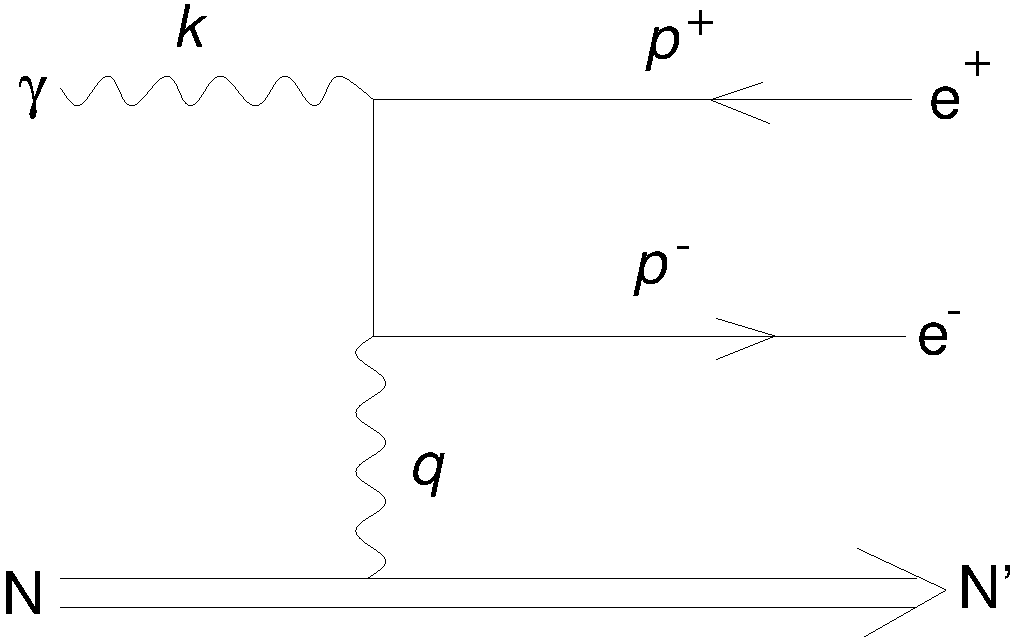
\includegraphics[height=8cm,width=12cm]{figures/pair}
\caption{\label{pair_fig} Feynman diagram for the pair
production process}
%\end{center}
\end{figure}
The triplet production process is similar but the interaction
takes place with one of the atomic electrons which receives
sufficient energy to be set free (so that there are 3 secondary electrons
produced in the interaction). By default
the triplet production process is
\index{triplet production}
not simulated explicitly but taken into account in an approximate
way by using the total pair+triplet cross section to
sample distances to subsequent pair production collisions.
By default EGSnrc adopts the cross sections used in EGS4, {\em i.e.}
%total cross sections taken from ??? and
extreme relativistic first Born approximation
(Coulomb corrected above 50 MeV)
differential cross sections  as formulated in the article by
Motz, Olsen and Koch \cite{Mo69}. For a photon energy
$k$ incident on the nucleus with the atomic number $Z$, the
differential pair production cross section is
\begin{eqnarray}
\label{pair-e}
& & {{\rm d}\sigma_{\rm pair}(Z,k,E_+) \over {\rm d}E_+}  =
{A_{\rm p}'(Z,k) r_0^2 \alpha Z (Z + \xi(Z) ) \over k}
\\ & & \quad
\left\{ \left( E_+^2 + E_-^2 \right) \left[ \phi_1(\delta) -
{4 \over 3} \ln Z  - 4 \tilde{f}_c(k,Z) \right] +
{2 \over 3} E_+ E_- \left[ \phi_2(\delta) -
{4 \over 3} \ln Z  - 4 \tilde{f}_c(k,Z) \right] \right\}
\nonumber
\end{eqnarray}
where $E_+$ and $E_-$ are the total energies of the
positron and electron,
\begin{equation}
\delta = 136 Z^{-1/3} 2 \Delta~,\quad \quad \Delta = {k m \over 2 E_+ E_-}
\end{equation}
and $\tilde{f}_c(Z)$ is the Coulomb correction,
\begin{equation}
\label{f_coulomb}
\tilde{f}_c(Z) =
\begin{cases}
f_c(Z), & k \ge 50~\text{MeV} \\
0, & \text{else}
\end{cases}
\end{equation}
where $f_c(Z)$ was derived by
Davies, Bethe and Maximon \cite{Da54},
\begin{equation}
\label{f_coulomb1}
f_c(Z) = a^2 \sum_{\nu=1}^\infty {1 \over \nu (\nu^2 + a^2)}, \quad
a = \alpha Z~.
\end{equation}
The empirical correction factor $A_{\rm p}'(k,Z)$ is
introduced in order to improve the total pair production
cross section at lower energies and is defined
as ``The best estimate of the total cross section
available divided by the total cross section resulting
from the integration of Eq. (\ref{pair-e}) with
$A_{\rm p}'(k,Z)=1$''. For energies above
50 MeV $A_{\rm p}'$ is taken to be unity, for
energies below 50 MeV the total pair+triplet cross sections compiled
by Storm and Israel \cite{SI70} are used.
The replacement $Z^2 \to Z (Z + \xi(Z))$ takes
into account the triplet production process, where $\xi(Z)$,
evaluated by the PEGS4 function {\tt XSIF},  is given by
\index{XSIF}
\begin{equation}
\xi(Z) = {L_{\rm rad}'(Z) \over L_{\rm rad}(Z) - f_c(Z)}
\end{equation}
where $f_c(Z)$ is defined in Eq. (\ref{f_coulomb}) and
$L,L'$ are Tsai's radiation logarithms \cite{Ts74},
\index{Tsai's radiation logarithms}
\begin{eqnarray}
L_{\rm rad}'(Z) & = &
\left\{
\begin{array}{r@{\quad , \quad}l}
\ln(1194\,Z^{-2/3}) &~~\mbox{if}~~~Z > 4 \\
6.144 & ~~\mbox{if}~~~Z = 1 \\
5.621 & ~~\mbox{if}~~~Z = 2 \\
5.805 & ~~\mbox{if}~~~Z = 3 \\
5.924 & ~~\mbox{if}~~~Z = 4
\end{array} \right. \nonumber \\
L_{\rm rad} & = &
\left\{
\begin{array}{r@{\quad , \quad}l}
\ln(184.15\,Z^{-1/3}) &~~\mbox{if}~~~Z > 4 \\
5.310 & ~~\mbox{if}~~~Z = 1 \\
4.790 & ~~\mbox{if}~~~Z = 2 \\
4.740 & ~~\mbox{if}~~~Z = 3 \\
4.710 & ~~\mbox{if}~~~Z = 4
\end{array} \right.
\end{eqnarray}
The functions $\phi_1(\delta)$ and $\phi_2(\delta)$, which
account for screening effects, are
given by
\begin{equation}
\begin{split}
\phi_1(\delta) & = 4 \int\limits_\Delta^1 {{\rm d}q \over q^3}
(q - \Delta)^2 \Big[1 - F(q,Z) \Big]^2 + 4 + {4 \over 3} \ln Z~,
\\
\phi_2(\delta) & = 4 \int\limits_\Delta^1  {{\rm d}q \over q^4}
\Big[q^3 - 6 \Delta^2 q \ln \left({q \over \Delta}\right) + 3 \Delta^2 q
-4 \Delta^3 \Big] \Big[1 - F(q,Z) \Big]^2 + {10 \over 3} + {4 \over 3} \ln Z
\end{split}
\end{equation}
where $q$ is the momentum transfer and $F(q,Z)$ the corresponding
atomic form factor for an atom with atomic
number $Z$. For a Thomas-Fermi potential $\phi_1(\delta)$
and $\phi_2(\delta)$ are independent of $Z$ and Butcher and
Messel have approximated them \cite{BM60} as
\begin{eqnarray}
\label{pair_phi}
\phi_1(\delta) & = & \left\{
\begin{array}{r@{\quad , \quad}l}
20.867 - 3.242 \delta + 0.625 \delta^2 & \delta \le 1 \\
21.12 - 4.184 \ln(\delta + 0.952) & \delta > 1
\end{array}
\right. \\
\phi_2(\delta) & = & \left\{
\begin{array}{r@{\quad , \quad}l}
20.029 - 1.93 \delta - 0.086 \delta^2 & \delta \le 1 \\
\phi_1(\delta) & \delta > 1
\end{array}
\right.
\end{eqnarray}

The differential pair production cross section for compounds
and mixture is derived from the independent atom approximation
and can be approximately written in the same form as Eq. (\ref{pair-e})
but replacing
\begin{eqnarray}
\label{pair_replace}
Z (Z + \xi(Z)) \quad & \mbox{with} & \quad Z_{\rm eff}^2 \equiv
\sum p_i Z_i (Z_i + \xi(Z_i) )
\nonumber \\
{1 \over 3} \ln Z + \tilde{f}_c(k,Z) \quad & \mbox{with} & \quad
Z_V \equiv \sum p_i
Z_i (Z_i + \xi(Z_i) ) \left[ {1 \over 3} \ln Z_i + \tilde{f}_c(k,Z_i) \right]
\nonumber \\
\delta \quad & \mbox{with} & \quad \delta_C 2 \Delta~,\quad
\delta_C \equiv {136 \over Z_{\rm eff}^2}
\sum p_i Z_i (Z_i + \xi(Z_i) ) Z_i^{-1/3}
\end{eqnarray}
where $p_i$ is the normalized fraction of atoms of type $i$ in
the molecule.

It is worth noticing that, due to the use of the extreme
relativistic approximation,  the differential cross
section as defined in Eq. (\ref{pair-e}) becomes inaccurate
for energies close to the threshold energy for pair production
(2 $\rm m$ ).
%and breaks down altogether for energies below
%2.1 MeV.
In the EGS4 implementation, the entire photon energy
was given to one of the pair particles for $k \le 2.1$ MeV.
We have defined a macro {\tt \$SELECT-LOW-ENERGY-PAIR-PRODUCTION}
which, in its default replacement, samples $E_+$ uniformly
in the allowed range $m \cdots k/2$. If the user is aware
of a better approach, this simplistic treatment can be
modified by the appropriate replacement of this macro.
\index{\$SELECT-LOW-ENERGY-PAIR-PRODUCTION}

\paragraph{NRC pair cross sections}\hfill
\index{pair cross sections!NRC}

In a more recent addition to EGSnrc, the user has the option
to specify use of a library of differential pair cross sections created
at the NRC. These cross sections are based on the exact partial-wave-analysis
calculations by {\O}verb{\o}, Mork and Olsen (OMO) \cite{Ov73} for the
unscreened nuclear potential modified by a multiplicative screening correction.
The main difficulty in creating this data library, which provides cross
sections up to 85 MeV for all elements between 1 and 100, consisted in finding
numerically stable approaches for performing the PWA summation for energies
above a few MeV (the OMO paper \cite{Ov73} only contains results up to 5.1 MeV).
Note that these cross sections take into account the asymmetry in the
positron-electron energy distribution and eliminate the need
for the {\tt \$SELECT-LOW-ENERGY-PAIR-PRODUCTION} macro mentioned
above.

In order to make use of the NRC pair cross sections, the user
\index{pair\_nrc}
must set the variable {\tt pair\_nrc}=1.  Note that
{\tt pair\_nrc} is part of the {\tt COMIN/BREMPR} common block
(see Section~\ref{common_blocks} of this report).

\paragraph{Explicit simulation of triplet production}\hfill
\index{triplet production}

In a more recent addition to EGSnrc, the user has the option
to explicitely simulate triplet production events according to the
first Born approximation result first derived by Votruba \cite{Vo48}
and later by Mork \cite{Mo67}. Due to the 3 particle final state the
expression for the differential triplet production cross section
is very complicated and so not reproduced here. It is worth
noting that the published expressions most likely contain typos
because their direct implementation in a computer program
lead to meaningless results ({\em e.g.} negative cross section within
the kinematically allowed range of energies and directions).
The triplet production cross section was therefore re-derived using
the CompHEP package, its results were manipulated using Mathematica and
were then output directly to Fortran code.

In order to turn on explicit simulation of triplet events, the user
\index{itriplet}
mist set the variable {\tt itriplet}=1. Note that
{\tt itriplet} is part of the {\tt COMIN/BREMPR} common block
(see Section~\ref{common_blocks} of this report).

The technique for sampling random directions and energies from
the differential triplet cross section is very involved.
Its detailed description awaits a future version of this report.


\paragraph{Simulation of pair production, particle energies}\hfill
\index{pair production!simulation of}

When the NRC pair differential cross section tabulations are used,
an alias table is employed for picking the positron energy.
For the default Bethe-Heitler cross sections,
the sampling algorithm implemented in EGS4 becomes extremely
inefficient as the incident photon energy approaches the
threshold energy. This is due to the following two facts:
(i) The electron and positron energies, $E_-$ and $E_+$,
are sampled in the range $0\cdots k/2$, the allowed
range becomes a small fraction of the above interval for
$k \to 2 m$. (ii) The rejection functions used are normalized
to their maximum at $\delta = 0$. For photon energies that
are not much larger than $2 m$ the actual possible maximum
is much smaller.

\index{EGS4}
We have therefore slightly modified the EGS4 pair production sampling algorithm to improve
its efficiency. If we define the functions
\begin{eqnarray}
B(\delta) & = & 3 \Big[ \phi_1(\delta) - 4 Z_V \Big] -
\Big[ \phi_2(\delta) - 4 Z_V \Big] \nonumber \\
C(\delta) & = & 3 \Big[ \phi_1(\delta) - 4 Z_V \Big] +
\Big[ \phi_2(\delta) - 4 Z_V \Big]
\end{eqnarray}
which will serve as rejection functions, and make
a change of variables,
\begin{equation}
\varepsilon  = {E_+ - m \over k - 2 m}~,
\end{equation}
the differential pair production cross section can be
rewritten as
\begin{equation}
{{\rm d} \sigma_{\rm pair} \over {\rm d} \varepsilon} =
N \left\{ {B(\delta) \over B_{\rm max}} + \left(1 - {2 m \over k} \right)^2
{A_{\rm max} \over 3 B_{\rm max}} A(\delta)
\left[ 12 \left(\varepsilon - \frac{1}{2} \right)^2 \right] \right\}
\end{equation}
where $N$ combines all constant factors that are irrelevant for
the sampling algorithm and $A_{\rm max}$ and $B_{\rm max}$ are
the maxima of the rejection functions $A(\delta)$ and $B(\delta)$,
\begin{equation}
A_{\rm max} = A\left({4 \delta_C m \over k}\right)~, \quad \quad
B_{\rm max} = B\left({4 \delta_C m \over k}\right)~.
\end{equation}
The sampling algorithm, which determines the energy
of the lower energy ``electron'' is then as follows:
\begin{enumerate}
\item
Calculate $A_{\rm max}$, $B_{\rm max}$ and $\alpha$,
\begin{equation}
\alpha = {1 \over 1 + (1 - 2 m/k)^2 A_{\rm max}/3/B_{\rm max}}
\end{equation}
To save time at high energies, use $A_{\rm max} = A(0)$ and
$B_{\rm max} = B(0)$ for $k \ge 50$~MeV.
\item
Draw a random number $r_1$
\item
If $r_1 > \alpha$, then sample $\varepsilon$
from $12 (\varepsilon - 1/2 )^2$, {\em i.e.}
\begin{equation}
\varepsilon = \frac{1}{2} \left(1 - \mbox{Max}\{r_2,r_3,r_4\}\right)
\end{equation}
and use $A(\delta)/A_{\rm max}$ as a rejection function in step 5
\item
Else, sample $\varepsilon$ uniformly, {\em i.e.}
\begin{equation}
\varepsilon = \frac{1}{2} r_2
\end{equation}
and use $B(\delta)/B_{\rm max}$ as a rejection function in step 5
\item
Calculate $\delta$ and the rejection function $R$ = $A(\delta)/A_{\rm max}$ or
$B(\delta)/B_{\rm max}$
\item
If $r_5 < R$, accept $\varepsilon$, else go to step 2.
\end{enumerate}

\begin{figure}[h]
%\setlength{\vsize}{12cm}
%\setlength{\abovecaptionskip}{0.5in}
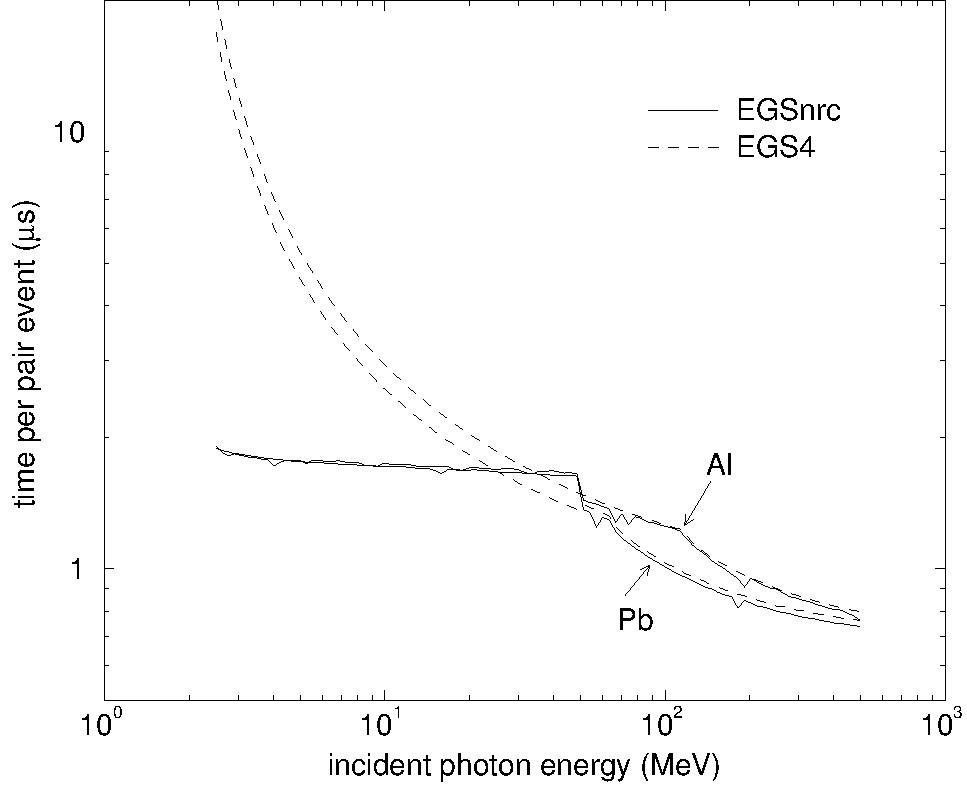
\includegraphics[height=12cm,width=12cm]{figures/pair_times}
\caption[CPU time for pair sampling]{\label{pair_times}
CPU time in $\mu$s on a 500 MHz PIII computer to sample a pair energy.}
\end{figure}

Fig. \ref{pair_times} shows the CPU time in $\mu$s on a 500 MHz PIII computer
running Linux necessary to sample a pair energy using the
algorithms discussed here (solid lines) and the original EGS4
algorithm (dashed lines) for aluminum and lead as a function
of the incident photon energy (this is just the time for
energy sampling, excluding angle sampling and rotations). Note
the logarithmic scale and the dramatic increase in CPU time for
the EGS4 algorithm and a photon energy less then 20 or 30 MeV.
The discontinuity in the EGSnrc algorithm around $50$~MeV
is due change in the
approach to calculate $A_{\rm max}$ and $B_{\rm max}$  (see item 1).

\paragraph{Simulation of pair production, particle angles}\hfill
\index{pair production!angular distribution}

\index{Bielajew, Alex} \index{EGS4}
In the original EGS4 version electrons and positrons were
produced at a fixed polar angle $\theta_{\pm}$ with respect to the direction
of the incoming photon given by $\theta_{\pm}=m/k$. This approach
was subsequently improved as discussed in PIRS Report 0287
\cite{Bi91} which introduced the {\tt \$SET-PAIR-ANGLE} macro
as an NRC extension to the EGS4 system.
This macro is now included in the EGSnrc system. The angle
selection procedure is controlled by the variable
{\tt IPRDST} (part of the {\tt COMIN/EDGE} common block--
see Section~\ref{common_blocks}) which can assume the following values:
\index{IPRDST}
\begin{itemize}
\item[]{\tt IPRDST=0}: The original EGS4 approach is used,
{\em i.e.} $\theta_{\pm}=m/k$
\item[]{\tt IPRDST=1}: The leading order term of the angular distribution
is employed, {\em i.e.}
\begin{equation}
\label{pair_ang1}
{{\rm d} \sigma \over {\rm d} \Omega_\pm} = N
{1 \over (1 - \beta_\pm \cos \theta_\pm)^2}
\end{equation}
where $N$ is again a normalization constant and $\beta_\pm$ denotes
the velocity of the positron or electron in units of the speed of light.
\item[]{\tt IPRDST=2}: The formula 3D-2003 of the article by
Motz {\em et al.} \cite{Mo69} is used, which is the cross section, differential
\index{IPRDST}
in electron/positron energy and angle:
\end{itemize}
\begin{equation}
\label{pair_ang_2}
\begin{split}
{{\rm d} \sigma \over {\rm d} E_\pm {\rm d} \Omega_\pm} & =
{N \over (u^2+1)^2 }
\left\{ -(E_+ - E_-)^2 - {16 u^2 E_+ E_- \over (u^2 + 1)^2} +
\left[ E_+^2 + E_-^2 + {4 u^2 E_+ E_- \over (u^2 + 1)^2} \right]
\ln M(k,E_\pm,u) \right\} \\
u & =  E_\pm \theta_\pm~, \quad {1 \over M(k,E_\pm,u)} =
\left({k \over 2 E_+ E_-} \right)^2 + \left( { Z_{\rm eff}^{1/3} \over
111 (u^2 + 1)^2 } \right)^2
\end{split}
\end{equation}
\begin{itemize}
\item[\phantom{\tt IPRDST=2}]
where all energies are measured in units of $m$.
Note that Eq. (\ref{pair_ang_2}) is based on an extreme relativistic,
small angle approximation where
\begin{equation}
\begin{split}
(1 - \beta_\pm \cos \theta_\pm)^2 & \approx
\left[1 - \beta_\pm \left(1 - \frac{\theta_\pm^2}{2}\right) \right]^2
= (1 - \beta_\pm)^2 \left[ 1 - {\beta_\pm \over 1 - \beta_\pm}
\frac{\theta_\pm^2}{2} \right]^2 \\
& \approx  (1 - \beta_\pm)^2 (1 + u^2)^2~.
\end{split}
\end{equation}
Perhaps, it would be a good idea to replace $1+u^2$ with
$1 - \beta_\pm \cos \theta_\pm$ in the denominator outside
of the curled brackets of Eq. (\ref{pair_ang_2}), but
we have not undertaken this modification.
\end{itemize}

The sampling algorithm for Eq. (\ref{pair_ang_2}) is discussed
extensively in Ref. \cite{Bi91}.
\index{Bielajew, Alex}
%.
It should be noted that
this algorithm becomes progressively more inefficient with
increasing energies. Given this fact and the approximations
involved which make its use questionable at low energies,
we have chosen {\tt IPRDST=1} as the default
pair angle selection scheme in EGSnrc. The generation
of electron and positron polar angles from the
distribution (\ref{pair_ang1}) is trivial, it
is accomplished by
\index{IPRDST}
\begin{equation}
\cos \theta_\pm = {2 r - 1 + \beta_\pm \over \beta_\pm (2 r -1 ) + 1}
\end{equation}
where $r$ is an uniformly distributed random number between zero and
unity. As pair-production is a three-body process, separate polar
angles for the electron and positron are needed. The two
azimuthal angles are chosen to be opposite. This is,
strictly speaking, not correct, but due to lack of a better
alternative, adopted from the original EGS4 version.

\paragraph{Russian Roulette for pair production events} \hfill
\index{Russian Roulette}
\index{variance reduction!Russian Roulette}
\index{pair production!Russian Roulette}

It is wasteful to simulate all pair production events if
the user intends to play Russian Roulette with electrons
set in motion in photon interactions. We have therefore implemented
an EGSnrc internal Russian Roulette scheme which is turned on
by setting the flag {\tt i\_play\_RR} which is in {\tt
COMIN/EGS-VARIANCE-REDUCTION/}
to 1. The survival probability for the electrons is
{\tt prob\_RR}, also in {\tt COMIN/EGS-VARIANCE-REDUCTION/}.
If {\tt i\_play\_RR} is set, the following actions are
taken at the beginning of subroutine {\tt PAIR}:
\index{EGS-VARIANCE-REDUCTION}
\index{prob\_RR} \index{i\_play\_RR}
\begin{enumerate}
\item
Pick a random number $r$
\item
If $r > $~{\tt prob\_RR}, reduce the stack size by one, return
to {\tt PHOTON} ({\em i.e.} save the simulation of the pair event).
If the stack becomes empty, a zero weight, zero energy photon
is left on the stack so that the {\tt PHOTON} routine can exit
properly.
\item
If $r < $~{\tt prob\_RR}, increase the weight of the current photon by
1/prob\_RR and simulate the pair event as usual.
\end{enumerate}
For more discussion of Russian Roulette see sections~\ref{rusrou} and
\ref{step_5b}.

\subsubsection{Incoherent (Compton) scattering}
\setcounter{equation}{0}
\label{compton}
\index{bound Compton scattering}
\index{Compton scattering}
\index{incoherent scattering}
\index{cross section!incoherent}

\paragraph{Cross section}\hfill

The Feynman diagram for the Compton scattering process is
shown in Fig. \ref{compt_fig}. The circle in the line
of the incoming atom A indicates that the electron
\begin{figure}[h]
%\begin{center}
%\setlength{\hsize}{15cm}
%\setlength{\vsize}{8cm}
%\setlength{\abovecaptionskip}{0.5in}
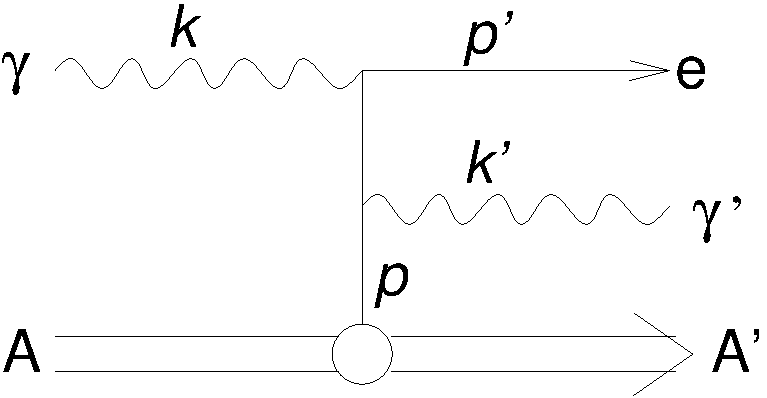
\includegraphics[height=8cm,width=12cm]{figures/compt}
\caption{\label{compt_fig} Feynman diagram for the Compton process}
%\end{center}
\end{figure}
is initially bound to the atom and represents the probability
that an atomic electron with a four-momentum $p = (E,\vec{p})$
interacts with the incoming photon with a four-momentum
$k=(k,\vec{k})$ into a final $e^-\gamma'$ state given by
$k'=(k',\vec{k'})$ and $p'=(E',\vec{p}')$.
To simplify the notation, all energies will be measured
in units of the electron's rest energy $m$ and all momenta
in units of $m/c$ in the following equations of this
section.

\index{Klein-Nishina}
If the binding to the atom is neglected and the electron
is considered to be initially at rest ({\em i.e} $p = (1,0,0,0)$),
the cross section for the process is given by the Klein-Nishina
formula \cite{KN29},
\begin{equation}
{{\rm d} \sigma_{\rm KN} \over {\rm d} \cos \theta} = \pi r_0^2 Z~
X_{\rm KN}~, \quad \quad X_{\rm KN} =
\left({k_c \over k} \right)^2
\left[ {k_c \over k} + {k \over k_c} - \sin^2 \theta \right]
\end{equation}
where $\theta$ is the polar angle of the scattered photon with
respect to the initial direction and $k_c$ is the energy
of a photon scattered at an angle $\theta$
by free electrons at rest,
\begin{equation}
k_c = {k \over 1 + k (1 - \cos \theta)}
\end{equation}
\index{Doppler broadening}
\index{incoherent scattering!binding effects}
\index{incoherent scattering!Doppler broadening}
The treatment of the Compton process in EGS4 is based on these
equations with $k' = k_c$. In EGSnrc we have included binding effects and
Doppler broadening according to the impulse approximation (IA)
\cite{Ri75}. The IA assumes that the potential in which the
target electrons move is constant so that their states can
be represented by plane waves. The double differential
cross section for photon scattering into the final state
$k' = (k', k' \sin \theta \cos \phi, k' \sin \theta \sin \phi, \\
k' \cos \theta)$ is given by (Eq. (15) of Ref. \cite{RB82})
\begin{equation}
\label{comp_cs1}
{{\rm d}^2 \sigma_{\rm comp} \over {\rm d}k' {\rm d}\Omega} =
{r_0^2 \over 2} {k' \over k q} \Big[1 + p_z^2 \Big]^{-1/2} X J(p_z)
\end{equation}
where $\Omega$ is the solid angle $(\theta,\phi)$ and where
\begin{itemize}
\item
$q$ is the modulus of the momentum transfer vector
$\vec{q} = \vec{k'} - \vec{k}$,
\begin{equation}
q = \sqrt{k^2 + k^{\prime 2} - 2 k k' \cos \theta}
\end{equation}
\item
$p_z$ is the projection of the initial electron momentum
on the direction of $\vec{q}$,
\begin{equation}
\label{comp_pz}
p_z = {\vec{p} \cdot \vec{q} \over q} =
{k k' (1 - \cos \theta) - k + k' \over q}
\end{equation}
Note that the above equation is derived from a non-relativistic
approximation and requires $|p_z| \le 1$.
\item
$X$ is defined as
\begin{eqnarray}
X & = & {R \over R'} + {R' \over R} +
2 \left(\frac{1}{R} - \frac{1}{R'} \right)
+ \left(\frac{1}{R} - \frac{1}{R'} \right)^2 \nonumber \\
R & = & k \left[ \sqrt{1 + p_z^2} + {k - k' \cos \theta \over q} p_z \right]
\nonumber \\
R' & = & R - k k' (1 - \cos \theta)~.
\end{eqnarray}
Note that $R$ and $R'$ simplify to
\begin{equation}
R \approx k \left(1 + O(p_z) \right)~, \quad
R' \approx k \Big[1 - k_c (1 - \cos \theta ) \Big] \left(1 + O(p_z) \right)
\end{equation}
for $p_z \ll 1$. In this limit
\begin{equation}
X = X_{\rm KN} \left(1 + O(p_z) \right)
\end{equation}
\item
The function $J(p_z)$ is the Compton profile,
\begin{equation}
J(p_z) = \int {\rm d} p_x {\rm d} p_y | \psi(\vec{p}) |^2~,
\end{equation}
where $\psi(\vec{p})$ is the wave function of the bound electrons.
Extensive tables of atomic and shell-wise
\index{Compton profiles}
\index{incoherent scattering!Compton profiles}
Hartree-Fock Compton profiles for all
elements have been published by Biggs {\em et al} \cite{BM75}.
Following Brusa {\em et al} \cite{BS96},
contributions
from different electron shells are considered separately, so
that the atomic or molecular Compton profile is the sum
of one-electron shell Compton profiles $J_i(p_z)$, and binding effects
are taken into account by rejecting interactions that
transfer less energy to the electron than the binding energy $U_i$,
{\em i.e.}
\begin{equation}
J(p_z) = \sum Z_i J_i(p_z) \Theta(k - k' - U_i)~.
\end{equation}
Here, $Z_i$ is the occupation number of shell $i$ and
the $J_i$ have the normalization
\begin{equation}
\int\limits_{-\infty}^\infty {\rm d} p_z J_i(p_z) = 1
\end{equation}
\end{itemize}
With all this, and after changing the cross section
from differential in $k'$ to differential in $p_z$,
Eq. (\ref{comp_cs1}) can be written as
\begin{equation}
{{\rm d}^2 \sigma_{\rm comp} \over {\rm d}p_z {\rm d}\Omega} =
{r_0^2 \over 2} X_{\rm KN}
\left( \sum Z_i J_i(p_z) \Theta(k - k' - U_i) \right) F(k,\cos \theta, p_z)
\end{equation}
where the function $F(k,\cos \theta, p_z)$ combines all remaining
factors times ${\rm d}k'/{\rm d}p_z$,
\begin{equation}
F(k,\cos \theta, p_z) = \frac{k'}{k_c} \Big[ 1 + p_z^2 \Big]^{-1/2}
\frac{X}{X_{\rm KN}} \left(1 + \frac{k_c}{k} {k \cos \theta - k' \over q} p_z
\right)^{-1}
\end{equation}
Here, $k'$ is a function of $k, \cos \theta$ and $p_z$ and
follows from solving Eq. (\ref{comp_pz}) with respect to $k'$,
{\em i.e.}
\begin{equation}
\label{comp_kprime}
k' = {k_c \over 1 - p_z^2 \varepsilon^2 } \left[
1 - p_z^2 \varepsilon \cos \theta + p_z \sqrt{1 - 2 \varepsilon
\cos \theta + \varepsilon^2 \left(1 - p_z^2 \sin^2 \theta \right) }~ \right]~,
\quad \quad \varepsilon = \frac{k_c}{k}
\end{equation}
The incoherent scattering cross section, differential in
the photon scattering angle, is
\begin{equation}
\label{comp_sig_omega}
{{\rm d} \sigma_{\rm comp} \over {\rm d}\Omega} =
{r_0^2 \over 2}
%\left(\frac{k_c}{k} \right)^2 : must not be there, noted by Trent Hawkins
X_{\rm KN} S(k,\cos \theta)
\end{equation}
where
\begin{equation}
\label{comp_sincoh}
S(k,\cos \theta) =
\sum Z_i \Theta(k - U_i) S_i, \quad \quad
S_i = \int\limits_{-\infty}^{p_i} {\rm d} p_z J_i(p_z)
F(k,\cos \theta, p_z)
\end{equation}
\index{incoherent scattering function}
can be identified with the incoherent scattering function.
The upper limit of the $p_z$ integration for the $i$'th shell, $p_i$,
\begin{equation}
\label{comp_pi}
p_i = { k (k - U_i) (1 - \cos \theta) - U_i \over
\sqrt{ 2 k (k - U_i) (1 - \cos \theta) + U_i^2}}~,
\end{equation}
follows from Eq. (\ref{comp_pz}) with
$k' = k - U_i$ and assures that sufficient energy is transferred
to the electron to set it free. To first order, $S(k,\cos \theta)$
depends only on $k \sqrt{(1 - \cos \theta)/2}$ and so,
Namito {\em et al} \cite{Na94} use tabulated
incoherent scattering functions in their
extension of the EGS4 system to include binding effects
and Doppler broadening, when sampling the photon scattering angle.
This approach introduces a slight inconsistency in their treatment
of the Compton process.

As the Compton profiles are
strongly peaked around $p_z=0$, the main contributions
to the integral come from small $p_z$ values where
the function $F(k,\cos \theta, p_z)$ is very close
to unity and so, Brusa {\em et al} \cite{BS96} approximate
$S(k,\cos \theta)$ with
\begin{equation}
\label{comp_sincoh1}
S(k,\cos \theta) \approx S_A((k,\cos \theta) \equiv
\sum Z_i \int\limits_{-\infty}^{p_i} {\rm d} p_z J_i(p_z)
\Theta(k - U_i)
\end{equation}
for their implementation of binding effects and Doppler broadening
in the PENELOPE system \cite{Sa96}\footnote{They take
into account $F(k,\cos \theta, p_z)$, using its Taylor
expansion up to $O(p_z)$, for the sampling of $p_z$.}
\begin{figure}[h]
%\begin{center}
%\setlength{\vsize}{12cm}
%\setlength{\abovecaptionskip}{0.5in}
\includegraphics[height=12cm,width=12cm]{figures/sincoh}
%\end{center}
\caption[Incoherent scattering function]{\label{comp_sincoh_fig}
The incoherent scattering function for lead and $k=50$~keV
calculated from Eq. (\protect\ref{comp_sincoh}) (solid line)
and from Eq. (\protect\ref{comp_sincoh1}) (dashed line)
by numerical integration}.
\end{figure}
This approach introduces a small error at low energies
for high $Z$ materials as can be seen
in Fig. \ref{comp_sincoh_fig} which shows
$S(k,\cos \theta)$ for 50 keV photons in lead calculated
with or without taking into account $F(k,\cos \theta, p_z)$.

To minimize the amount of data necessary for
the simulation of the Compton process, and to make
the calculation of the incoherent scattering function ``on the fly''
possible, we use
the analytical approximations for the Compton profiles
$J_i(p_z)$ proposed by Brusa {\em et al} \cite{BS96}:
\begin{equation}
\label{comp_Japprox}
J_i(p_z) = J_{i,0} (1 + 2 J_{i,0} |p_z| ) \exp\left[\frac{1}{2} -
\frac{1}{2}\left(1 + 2 J_{i,0} |p_z| \right)^2\right]
\end{equation}
where $J_{i,0} \equiv J_i(0)$ is the value of the profile at
$p_z = 0$ obtained from the Hartree-Fock orbital \cite{BM75}.
In addition, we approximate $F(k,\cos \theta, p_z)$ by
\begin{equation}
\label{comp_Fapprox}
F((k,\cos \theta, p_z) = \left\{
\begin{array}{l@{\quad , \quad}l}
1 - \alpha p & p_z \le -p \\
1 + \alpha p_z & |p_z| < p \\
1 + \alpha p & p_z \ge p
\end{array} \right.
\end{equation}
where
\begin{eqnarray}
\label{comp_alpha}
\alpha & = & \frac{q_c}{k} \left(1 +
{k_c (k_c - k \cos \theta) \over q_c^2} \right)
\nonumber \\
q_c & = & \sqrt{k^2 + k_c^2 - 2 k k_c \cos \theta}~.
\end{eqnarray}
Equation (\ref{comp_Fapprox}) results from a Taylor series
expansion of $F(k,\cos \theta, p_z)$ up to $O(p_z)$. As this
approximation becomes inaccurate for large $p_z$ values
it is applied only for $|p_z| < p$, else the function values at
$\pm p$ are used. We have checked by numerical integration
of Eq. (\ref{comp_sincoh}) that the incoherent scattering function
calculated with the approximation (\ref{comp_Fapprox}) agrees
to better than 0.3\% with the incoherent scattering function
calculated using the exact expression for $F(k,\cos \theta, p_z)$
if $p = 0.15$ is used.

Combining now Eq. (\ref{comp_sincoh}), (\ref{comp_Japprox}) and
(\ref{comp_Fapprox}),  we obtain for $S_i$
%\begin{equation}
%S_i(k,\cos \theta) = \left\{
%\begin{array}{l@{\quad , \quad}l}
%(1 - \alpha p) {e^{-b} \over 2} & p_z \le -p \\
%(1 + \alpha p_z) {e^{-b} \over 2} - {\alpha \over 4 J_{i,0}}
%\sqrt{{\pi \over 2}} e^{1/2} \left[ \mbox{Erf} \left( 1 + 2 J_{i,0} p \over
%\sqrt{2} \right) - \mbox{Erf} \left(  1 + 2 J_{i,0} |p_z|
%\over \sqrt{2} \right) \right] & -p < p_z \le 0  \\
%1 - (1 + \alpha p_z) {e^{-b} \over 2} - {\alpha \over 4 J_{i,0}}
%\sqrt{{\pi \over 2}} e^{1/2} \left[ \mbox{Erf} \left( 1 + 2 J_{i,0} p \over
%\sqrt{2} \right) - \mbox{Erf} \left(  1 + 2 J_{i,0} |p_z|
%\over \sqrt{2} \right) \right] & 0 < p_z < p \\
%1 - (1 + \alpha p) {e^{-b} \over 2} & p_z \ge p
%\end{array} \right.
%\end{equation}
\begin{eqnarray}
\label{comp_Si}
& & S_i(k,\cos \theta) \nonumber \\
& = & (1 - \alpha p) {e^{-b} \over 2}~,\quad \mbox{if}~~p_i \le -p \nonumber \\
& = &
(1 + \alpha p_i) {e^{-b} \over 2} - {\alpha \over 4 J_{i,0}}
\sqrt{{\pi \over 2}} e^{1/2} \left[ \mbox{Erf} \left( 1 + 2 J_{i,0} p \over
\sqrt{2} \right) - \mbox{Erf} \left(  1 + 2 J_{i,0} |p_i|
\over \sqrt{2} \right) \right]~,\quad \mbox{else if}~~ p_i \le 0 \nonumber \\
& = &
1 - (1 + \alpha p_i) {e^{-b} \over 2} - {\alpha \over 4 J_{i,0}}
\sqrt{{\pi \over 2}} e^{1/2} \left[ \mbox{Erf} \left( 1 + 2 J_{i,0} p \over
\sqrt{2} \right) - \mbox{Erf} \left(  1 + 2 J_{i,0} |p_i|
\over \sqrt{2} \right) \right] ~,\quad \mbox{else if}~~ p_i < p \nonumber \\
& = &
1 - (1 + \alpha p) {e^{-b} \over 2} ~,\quad \mbox{else}
\end{eqnarray}
where
\begin{equation}
b = \frac{1}{2}\left(1 + 2 J_{i,0} |p_i| \right)^2 - \frac{1}{2}
\end{equation}
and $\mbox{Erf}$ is the error function. It is worth noticing that
$S_i$ is always less or equal to unity. This fact allows for
using it as a rejection function in the sampling algorithm discussed
in the next section.

The total incoherent scattering cross section $\sigma_{\rm comp}^{\rm (tot)}$
can be obtained
by a numerical integration over all scattering angles from
Eq. (\ref{comp_sig_omega}), (\ref{comp_sincoh}) and
(\ref{comp_Si}). To
avoid substantial changes of the data preparation program PEGS4,
we use instead the total Klein-Nishina cross section,
$\sigma_{\rm KN}^{\rm (tot)}$, while tracking the photons through
the geometry, and reject Compton interactions with the probability
$1-\sigma_{\rm comp}^{\rm (tot)}/\sigma_{\rm KN}^{\rm (tot)}$ once
at the interaction site (fictitious cross section method).
This rejection probability results automatically (without
calculating $\sigma_{\rm comp}^{\rm (tot)}$) from the sampling
algorithm, as we shall see in the next section.

\index{IBCMP}
Another advantage of this approach is that the user can
turn on or off binding effects and Doppler broadening
using the switch {\tt IBCMP} (included in the common
block {\tt COMIN/COMPTON-DATA}--see Section~\ref{common_blocks}),
without preparing two
separate material data files. The only additional data
needed to simulate incoherent scattering in the impulse
approximation are the Compton profile parameters
$J_{i,0}$, taken from the tabulations by Biggs {\em et al}
\cite{BM75}, and the occupation numbers $Z_i$ and
binding energies $U_i$ for all elements, taken from
Lederer and Shirley \cite{LS78}. These data are read in
in subroutine {\tt init\_compton} which is called from
{\tt HATCH}.
\index{init\_compton}

\paragraph{Simulation of incoherent scattering events}\hfill
\index{incoherent scattering!simulation of}
\index{Compton scattering!simulation of}
\index{bound Compton scattering}

The incoherent scattering cross section, differential in
the photon scattering angle $\Omega = (\theta,\phi)$
and the Doppler broadening
parameter $p_z$, per interaction site sampled from the
total Klein-Nishina cross section is
\begin{eqnarray}
{{\rm d}^2 \sigma_{\rm comp} \over \sigma_{\rm KN}^{\rm (tot)}} & = &
\sum \frac{Z_i}{Z} \Theta(k - U_i)~ \sigma_i~ {\rm d} \Omega~ {\rm d} p_z
\\
\sigma_i~ {\rm d} \Omega~ {\rm d} p_z & = &
%\left( \int\limits_{-\infty}^{p_i} {\rm d} p_z J_i(p_z) F(k,\cos \theta,p_z)
%\right)~
S_i~
{{\rm d} \phi \over 2 \pi}~
{X_{\rm KN}(\cos \theta)~{\rm d} \cos \theta~ \over
\int\limits_{-1}^1 X_{\rm KN}(\cos \theta) {\rm d} \cos \theta }
~{ J_i(p_z) F(k,\cos \theta,p_z) \Theta(p_i - p_z) {\rm d} p_z \over
\int\limits_{-\infty}^{p_i} {\rm d} p_z J_i(p_z) F(k,\cos \theta,p_z) }
\nonumber
\end{eqnarray}
It is then clear that the following algorithm produces the
required number of rejections and samples the differential
cross section correctly, if the interaction is accepted:
\begin{enumerate}
\item
Sample the shell number $i$ using the probabilities $Z_i/Z$
\item
If the incident photon energy $k$ is smaller than the binding
energy $U_i$, reject the interaction,
else, sample $\cos \theta, \phi$ and $p_z$ using the differential
cross section $\sigma_i$ of the selected shell as follows:
\item
Sample the photon polar scattering angle $\theta$ using
\begin{displaymath}
P_1(\cos \theta) =
{X_{\rm KN}(\cos \theta)~{\rm d} \cos \theta~ \over
\int\limits_{-1}^1 X_{\rm KN}(\cos \theta) {\rm d} \cos \theta }
\end{displaymath}
which is a normalized probability distribution function (PDF). The method
for sampling $\cos \theta$ will be explained below.
\item
Calculate the maximum possible value of $p_z$, $p_i$, from
Eq. (\ref{comp_pi}), and $S_i$ from Eq. (\ref{comp_Si}).
\item
If a uniformly distributed random number is greater then $S_i$,
reject the interaction
\item
Sample $p_z$ from
\begin{displaymath}
P_2(p_z) =
{ J_i(p_z) F(k,\cos \theta,p_z) \Theta(p_i - p_z) {\rm d} p_z \over
\int\limits_{-\infty}^{p_i} {\rm d} p_z J_i(p_z) F(k,\cos \theta,p_z) }
\end{displaymath}
which is a normalized PDF for $p_z$. The sampling
technique employed for this distribution function is explained below.
\item
Sample the azimuthal scattering angle from ${\rm d}\phi/(2 \pi)$
\item
Calculate the energy $k'$ of the scattered photon from
Eq. (\ref{comp_kprime})
\item
The electron set in motion has then a kinetic energy of $k - k' - U_i$,
a polar scattering angle $\theta_e$ given by
\begin{equation}
\cos \theta_e = {k - k' \cos \theta \over
\sqrt{k^2 + k^{\prime 2} - 2 k k' \cos \theta} }
\end{equation}
and an azimuth opposite to the photon's azimuth.
\end{enumerate}
Note that if the user does not want to take into account binding
effects and Doppler broadening (the switch {\tt IBCMP} is set to zero)
the sampling algorithm consists of steps 3, 7 and 9 with
$k' = k_c$ and $U_i = 0$.
\index{IBCMP}

As the shell with which the interaction takes place is explicitly determined
in step 1, at the end of the sampling algorithm the vacancy created
by the Compton process is known. The relaxation of shell vacancies
\index{relaxations}
\index{atomic relaxations}
with binding energies above the specified transport threshold
energies is performed in subroutine {\tt relax} (see section \ref{relax}) and
may lead to the creation of additional fluorescent photons and
Auger and Coster-Kronig electrons on the stack. Many of the
EGS4 based user codes assume that the outcome of an incoherent scattering
process is a scattered photon and a Compton electron. This assumption
is obviously not satisfied for EGSnrc, the outcome of an incoherent
event may by any one of the following:
\begin{enumerate}
\item
The original photon, if the interaction was rejected due to the one
of the rejection criteria
\item
A scattered photon and a Compton electron, if all relaxation particles
had energies below the specified transport threshold energies
({\tt ECUT} and {\tt PCUT})
\item
A scattered photon, a Compton electron plus $n$ relaxation particles, else.
\end{enumerate}
See section~\ref{stack_status} (page~\pageref{stack_status}) for more
information.

Finally, the portion of the binding energy that resulted in the creation
of sub-threshold relaxation particles is made known to the user via
a call to the scoring routine {\tt AUSGAB} with the argument {\tt IARG=4}.
\index{AUSGAB}
\index{IARG!4}

We conclude this section with some details about steps 3, 4 and 6
of the sampling algorithm.

\underline{Step 3, sampling of $\cos \theta$}: Following
the EGS4 manual\cite{Ne85} we rewrite
the PDF $P_1$ in terms of $\varepsilon = k_c/k$,
\index{SLAC-265}
\begin{equation}
\label{comp_P1}
P_1(\varepsilon) = P_1(\cos \theta) {{\rm d}\varepsilon \over
{\rm d} \cos \theta} = N \left( \frac{1}{\varepsilon} + \varepsilon -
\sin^2 \theta \right)
\end{equation}
where $N$ is a normalization constant that is irrelevant for the sampling
algorithm. The minimum and maximum possible values for
$\varepsilon$, $\varepsilon_{\rm min}$ and $\varepsilon_{\rm max}$, follow
from $\cos \theta = -1$ and $\cos \theta = 1$, respectively, and are
given by
\begin{equation}
\varepsilon_{{\rm min}} = {1 \over 1 + 2 k}~, \quad \quad
\varepsilon_{{\rm max}} = 1~.
\end{equation}
Equation (\ref{comp_P1}) can be further rewritten as
\begin{equation}
P_1(\varepsilon) = N (\alpha_1 + \alpha_2) \left\{
{\alpha_1 \over \alpha_1 + \alpha_2}~
\left({1 \over \varepsilon \alpha_1} \right)
+ {\alpha_2 \over \alpha_1 + \alpha_2}~\left({ \varepsilon \over \alpha_2}
\right) \right\} \left[ 1 - {\varepsilon \sin^2 \theta \over 1 +
\varepsilon^2 } \right]
\end{equation}
with
\begin{equation}
\alpha_1  =  \ln \left(1 + 2 k \right)~, \quad \quad
\alpha_2  = {1 - \varepsilon_{\rm min}^2 \over 2}
\end{equation}
$1/\varepsilon/\alpha_1$ and $\varepsilon/\alpha_2$ are
normalized PDFs, they can be used to sample $\varepsilon$
with the probability $\alpha_1/(\alpha_1 + \alpha_2)$ and
$\alpha_2/(\alpha_1 + \alpha_2)$, respectively. The expression
of the square brackets has a maximum of unity for
$\varepsilon = 1$ ($\sin \theta = 0$) and is thus
a valid rejection function. The sampling algorithm is then as follows:
\begin{itemize}
\item[3.1]
Calculate $\varepsilon_{\rm min}, \alpha_1, \alpha_2$ and
$w = \alpha_1/(\alpha_1 + \alpha_2)$
\item[3.2]
Pick three random numbers $r_1, r_2$ and $r_3$
\item[3.3]
If $r_1 \le w$,
\begin{equation}
\varepsilon = \varepsilon_{\rm min} \exp( r_2 \alpha_1 )~,
\end{equation}
else,
\begin{equation}
\varepsilon = \sqrt{ \varepsilon_{\rm min}^2 + 2 r_2 \alpha_2}
\end{equation}
\item[3.4]
Calculate the rejection function ($g$), if $r_3 > g$ go to step 3.2
\item[3.5]
Deliver $\varepsilon$ (and $\cos \theta$)
\end{itemize}
The efficiency of this algorithm
goes to unity for $k \to \infty$ and therefore this is
the most efficient algorithm at high incident photon energies.
For $k \to 0$, the efficiency approaches $2/3$. In addition,
the necessity to calculate a logarithm and an exponential function,
two CPU intensive calculations, makes this algorithm slower than
a simple rejection technique with a uniform sampling of $\varepsilon$.
The rejection function in this case is given by
\begin{equation}
g = \frac{1}{g_{\rm max}} \left( {1 \over \varepsilon} + \varepsilon -
\sin^2 \theta \right)~, \quad \quad g_{\rm max} =
{1 \over \varepsilon_{\rm min}} + \varepsilon_{\rm min}
\end{equation}
and the algorithm is as follows
\begin{itemize}
\item[3.1]
Calculate $\varepsilon_{\rm min}$ and $g_{\rm max}$
\item[3.2]
Pick two random numbers $r_1$ and $r_2$
\item[3.3]
Set
\begin{equation}
\varepsilon = r_1 + (1 - r_1) \varepsilon_{\rm min}
\end{equation}
and calculate $g$
\item[3.4]
If $r_2 > g$, go to step 3.2
\item[3.5]
Deliver $\varepsilon$ (and $\cos \theta$)
\end{itemize}
The efficiency of this algorithm is $2/3$ for low energies and
decreases with increasing $k$. Because there are no CPU intensive
calculations involved, it is faster up to $k \sim 2$ and
used by EGSnrc in this energy range.

\underline{Step 4, calculation of $S_i$}: The calculation of
$S_i$ requires two numerically intensive operations, the
computation of $\exp(-b)$ and the calculation of the error
function that depends on $p_i$. The former is necessary for
the sampling of $p_z$ in step 6, the latter can be avoided
by using an approximate formula for $\mbox{Erf}$
(Eq. 7.1.25 of Abramowitz and Stegun \cite{AS64}):
\begin{eqnarray}
& & e^{1/2} \mbox{Erf} \left( { 1 + 2 J_{i,0} |p_i| \over \sqrt{2} } \right)
= e^{1/2} - e^{-b} t (a_1 + a_2 t + a_3 t^2 ) \\
t & = & {1 \over 1 + 0.332673 (1 + 2 J_{i,0} |p_i|)}~, \quad a_1 = 0.34802~,
\quad a_2 = -0.0958798~, \quad a_3 = 0.7478556 \nonumber
\end{eqnarray}
which is accurate enough for our purposes.

\underline{Step 6, sampling $p_z$}:
$p_z$ can be sampled using $J_i(p_z)$ as a PDF and $F$ as a rejection
function. To determine the maximum of $F$ we note that $\alpha$
(given by Eq. (\ref{comp_alpha})) is always positive except for
a small $\cos \theta$-range for $k > 3$. For such high incident
photon energies the influence of $F$ is negligible and so
we ignore it if $\alpha < 0$ ({\em i.e.} we set $\alpha = 0$).
The maximum of the rejection function, $F_{\rm max}$, is then
\begin{equation}
F_{\rm max} =
\label{comp_Fmax}
 \left\{
\begin{array}{l@{\quad , \quad}l}
1 - \alpha p & p_z \le -p \\
1 + \alpha p_i & |p_i| < p \\
1 + \alpha p & p_i \ge p
\end{array} \right.
\end{equation}
and the algorithm for sampling $p_z$ as follows:
\begin{itemize}
\item[6.1]
Calculate $F_{\rm max}$ from Eq. (\ref{comp_Fmax})
\item[6.2]
Pick two random numbers, $r_1$ and $r_2$, calculate $r' = r_1 e^{-b}$
($e^{-b}$ is known from step 4 of the main algorithm)
\item[6.3]
Set
\begin{equation}
p_z = \left\{ \begin{array}{l@{\quad , \quad}l}
{1 - \sqrt{1 - 2 \ln [2 r']} \over 2 J_{i,0}} & r' < 1/2 \\
{\sqrt{1 - 2 \ln [2(1-r')]} - 1 \over 2 J_{i,0}} & r' \ge 1/2
\end{array} \right.
\end{equation}
\item[6.4]
Calculate $F(p_z)$, if $r_2 > F(p_z)/F_{\rm max}$, go to step 6.2
\item[6.5]
Deliver $p_z$
\end{itemize}

It is easy to see that the sampling of incoherent scattering events
with binding effects and Doppler broadening taken into account
requires substantially more numerical work compared to
the free electron case (using the Klein-Nishina cross section).
\begin{figure}[h]
%\setlength{\vsize}{12cm}
%\setlength{\abovecaptionskip}{0.5in}
%\epsfxsize = 12cm
%\epsfysize = 12cm
\includegraphics[height=12cm,width=12cm]{figures/comp_times}
\caption[CPU times for Compton sampling]{\label{comp_times}
CPU time in $\mu$s on a 500 MHz PIII computer to sample an incoherent
scattering event (including necessary rotations of particle directions).}
\end{figure}
Fig. \ref{comp_times} shows the CPU time per incoherent scattering event
for EGS4 (solid line), EGSnrc without (dotted line)
and with binding effects (dashed line) as a function of the incident
photon energy. The long dashed line would result if the function
$F(k,\cos \theta,p_z)$ was ignored. EGSnrc without binding effects is
faster than EGS4 for low photon energies due to the use of
the uniform sampling technique. The inclusion of binding effects
increases the CPU time per Compton event by not more than a
factor of two and so has only a minor effect on the overall simulation
time when electron transport is included. Binding effects and
Doppler broadening for coherent scattering are therefore turned
on by default in the {\tt block data} sub-program (the switch
{\tt IBCMP} is set to 3, {\tt norej}).
\index{IBCMP}

Since the 2009 release of EGSnrc, the user has the option to change
the EGSnrc behavior with respect to Compton interactions by
setting {\tt ibcmp=2} or {\tt ibcmp=3}.
When {\tt ibcmp=2}, binding effects are taken into account via an
incoherent scattering function, but there is no Doppler broadening.
This option was mainly added for the sake of being able to study the
effect of Doppler broadening by comparing simulations with
{\tt ibcmp=2} to {\tt ibcmp=1}. To select this option the user
must set {\tt Bound Compton scattering} to {\tt simple} in the
{\tt MC TRANSPORT PARAMETER} input block.
The {\tt ibcmp=3} option is the same as {\tt ibcmp=1}, but now the actual total
bound Compton cross section
is used and there are no rejections at run time. The addition of this option
was motivated by the complications associated with the initial bound
Compton scattering approach when using an un-weighting technique to compute
ion chamber correction factors for photon attenuation.
To select this option the user
must set {\tt Bound Compton scattering} to {\tt norej} in the
{\tt MC TRANSPORT PARAMETER} input block.

\index{Russian Roulette}
\index{variance reduction!Russian Roulette}
\index{incoherent scattering!Russian Roulette}
If the Russian Roulette option is turned on {\tt i\_play\_RR} set
to 1, electrons produced as a result of the Compton interaction
(the Compton electron and electrons from the relaxation of
the shell vacancy) are removed from the stack with the probability
{\tt prob\_RR}. If they survive, their weight is increased by
1/{\tt prob\_RR}.

\paragraph{Radiative Compton corrections}\hfill
\index{radiative Compton corrections}
\label{radc_corrections}

Recently, the code has been modified to also allow the user to include
radiative corrections for Compton scattering in the one-loop approximation.
These corrections are based on the original
Brown \& Feynman equations \cite{BF52}. The effect of loop corrections is to
reduce the cross section at large photon scattering angles. This is partially
offset by the addition of the double-Compton scattering process (two photons in
the final state). Devising an efficient technique for sampling energies and
directions from the double-Compton cross section is the most difficult part
in the implementation. The method is quite involved and its detailed description
awaits a future version of this report.

In order to turn on radiative corrections, the input variable
\index{radc\_flag}
\texttt{radc\_flag} (in the common block \texttt{COMIN/COMPTON-DATA}) must be set to 1.
This option can be enabled in applications which can read the \texttt{MC transport parameter}
input block from an input file (\texttt{*.egsinp}) via the input key:
\begin{verbatim}
   Radiative Compton corrections = on
\end{verbatim}
Moreover, one must include the file \texttt{\$(EGS\_SOURCEDIR)rad\_compton1.mortran} to the
list of MORTRAN sources to be built just before \texttt{\$(EGS\_SOURCEDIR)get\_inputs.mortran}.
Depending on the application type this is accomplished in different ways:

\begin{itemize}
 \item
  For all C++ applications one must edit the file \texttt{\$HEN\_HOUSE/specs/egspp1.spec}
  and include the above file in the definition of the \texttt{C\_ADVANCED\_SOURCES}
  variable if the application is derived from the \texttt{EGS\_AdvancedApplication} class or the
  \texttt{C\_SIMPLE\_SOURCES} variable for any application derived from the \texttt{EGS\_SimpleApplication} class.
 \item
  For a specific C++ application one could define the variable \texttt{CPP\_SOURCES} in the application's
  \texttt{Makefile} in the same manner as done above for the \texttt{C\_ADVANCED\_SOURCES}.
 \item
  For a \texttt{BEAMnrc} application one must edit the file \texttt{sources.make} located in the application's
  folder and include the above file in the definition of the \texttt{SOURCES} variable
  or the \texttt{LIB\_SOURCES} variable if this \texttt{BEAMnrc} application will be used as a particle source for
  another application.
 \item
  For a MORTRAN application named for instance \texttt{app} one must edit the corresponding file app.make located
  in the application's folder \texttt{\$EGS\_HOME/app} and include the above file
  in the definition of the \texttt{SOURCES} variable.
\end{itemize}

% Note that if radiative Compton corrections are to be used then the \texttt{Makefile} of
% the user code must be modified to include the file \texttt{\$(EGS\_SOURCEDIR)rad\_compton1.mortran}
% in the \texttt{SOURCES} list, just before\\
% \texttt{\$(EGS\_SOURCEDIR)get\_inputs.mortran}.

\paragraph{Total Compton cross sections}\hfill
\label{comp_xsect}
\index{bound Compton scattering!user-supplied cross sections}

As mentioned above, the total Compton cross section used in EGSnrc is obtained
from the theoretical expressions by integration of the differential cross sections.
Another recent addition to the EGSnrc code allows the user to supply their
own cross sections for bound Compton scattering. This option is only available
if the user is simulating bound Compton scattering
\index{IBCMP}
({\tt IBCMP}=1,2,3).  The cross sections
must be contained in a file\\
 {\tt \$HEN\_HOUSE/data/comp\_xsections\_compton.data},
where {\tt comp\_xsections} is the variable
(in common block {\tt COMIN/MEDIA}) holding the name as supplied
by the user.
\index{comp\_xsections}

\subsubsection{Photo-electric absorption}
\setcounter{equation}{0}
\label{photo}
\index{photo-electric absorption}

In the photo-electric absorption process a photon is
absorbed by an atom and an electron
is emitted with an energy given by the incident photon
energy minus its binding energy.
The atom, left in an excited state with a vacancy in the
ionized shell, relaxes via the emission of fluorescent photons and
Auger and Coster-Kronig electrons.

\index{fluorescent X-rays}
In the original default EGS4 implementation the emission of relaxation
particles following photo-electric absorption events was
ignored. This approach was later modified
to include the production of $K_\alpha$ and $K_\beta$ fluorescent
radiation. However, for incident photon energies below
the $K$-shell binding energy, the entire photon energy is
deposited locally. Another shortcoming of the EGS4 approach is
that the $K$-shell binding energy is always subtracted
from the energy of the electron set in motion, even though there
is a certain probability that the photo-absorption process
takes place with a shell other than the $K$-shell (for
high-$Z$ materials this probability is of the order of 20\%).
Finally, the use of the fluorescent option in EGS4 requires
the user to select an ``effective'' atomic number for each
material. The photo-absorption then always takes place with
this atomic number. The meaningful selection of an
``effective'' $Z$ proves to be a difficult task for mixtures, especially
when only a small fraction of a high-$Z$ element is present.

\index{cross section!photo-electric absorption}
Although this release of EGSnrc uses the total photo-absorption
cross sections from PEGS (which are taken from the
compilation by Storm and Israel \cite{SI70})
the simulation of the photo-absorption process
is completely changed and is controlled
by the flag {\tt IEDGFL}
(in the {\tt COMIN/EDGE} common block-see Section~\ref{common_blocks}). If {\tt IEDGFL} of the
region is non-zero, a detailed simulation is performed,
otherwise a simplified treatment of the photo-absorption process
is undertaken. The default setting of {\tt IEDGFL} is 1.
\index{IEDGFL}

\paragraph{Detailed simulation of photo-electric absorption}\hfill
\label{photo_detailed}
\index{photo-electric absorption!detailed simulation of}

\begin{enumerate}
\item
For compounds and mixtures, the first step is to sample the
atomic number of the element the
photon is interacting with.
If $Z_i$ denotes the atomic number of the $i$'th element in
the molecule, $p_i$ its stoichiometric index, and
$\sigma_{\rm ph}(k,Z)$ the photo-electric absorption
cross section for a photon of energy $k$ by an element
with atomic number $Z$, then the probability $w_i(k)$ that
the photon is absorbed by the element $Z_i$ is
\begin{equation}
w_i = {p_i \sigma_{\rm ph}(k,Z_i) \over \sum p_i \sigma_{\rm ph}(k,Z_i)}~.
\end{equation}
The sampling of the element therefore requires the knowledge of
all elemental photo-absorption cross sections at run time, not
just the total photo-absorption cross sections that comes from
the PEGS data set. To minimize the amount of additional data
required, we use fit formulas for the $\sigma_{\rm ph}(k,Z_i)$'s
which are accurate to within 1-2\% and have the form
\begin{eqnarray}
\sigma_{\rm ph}(k,Z) & = & \frac{A_K(Z)}{k} + \frac{B_K(Z)}{k^2} +
\frac{C_K(Z)}{k^{7/2}} + \frac{D_K(Z)}{k^4}~, \quad \mbox{if}~k \ge U_K(Z)
\\
%& = & \exp \left[A_j(Z) + B_j(Z) \ln k + C_j(Z) (\ln k)^2 + D_j(Z) (\ln k)^3
%\right]~, \quad \mbox{else if}~k \ge U_j(Z)
& = & \exp \left[A_j(Z) + B_j(Z) t + C_j(Z) t^2 + D_j(Z) t^3
\right]~, \quad \mbox{else if}~k \ge U_j(Z)
\nonumber
\end{eqnarray}
where $t = \ln k$ and where $U_K(Z)$ is the
$K$-shell binding energy and $U_j(Z)$ binding
energies for shells other then the $K$-shell. We have obtained The
coefficients $A_K, B_K, ...$ and $A_j, B_j, ...$
by fitting the photo-absorption cross sections from the {\tt XCOM} program
\cite{BH87} and are found in the file {\tt photo\_cs.data}
(only shells with a binding energy above 1 keV are included).
The algorithm to select the element that absorbs the
incident photon is then:
\begin{itemize}
\item[1.1] Calculate all $\sigma_{\rm ph}(k,Z_i)$ and
their sum
\item[1.2] Pick a random number $r_1$
\item[1.3] In a loop over the number of elements, calculate
$r_1 = r_1 - w_i$, if $r_1 \le 0$ exit the loop and take
$Z_i$ as the element interacting with the photon.
\end{itemize}
Note that, at least in principle,
\begin{displaymath}
\sum p_i \sigma_{\rm ph}(k,Z_i) = \sigma_{\rm ph}(k)
\end{displaymath}
where $\sigma_{\rm ph}(k)$ is the photo-absorption cross section
for the material under consideration. This cross section is
interpolated using the PEGS supplied data in the photon
transport routine in order to determine
the interaction type. One could make the element selection algorithm
more efficient by employing
\begin{itemize}
\item[1.1']
Pick a random number $r_1$
\item[1.2']
Set $i=1$
\item[1.3']
Calculate $\sigma_{\rm ph}(k,Z_i)$ and
$r_1 = r_1 - p_i \sigma_{\rm ph}(k,Z_i)/\sigma_{\rm ph}(k)$.
\item[1.4'] If $r_1 > 0$ and $i$ less then the number of elements,
then $i = i+1$, go to step 1.3'.
\item[1.5'] Deliver $i$.
\end{itemize}
as this saves the evaluation of one or more $\sigma_{\rm ph}(k,Z_i)$
(especially if elements are ordered by decreasing probability for
photo-absorption prior to the actual simulation). We have not
implemented this more efficient algorithm as the photo-absorption
cross section interpolated using the PEGS supplied data becomes
inaccurate around absorption edges. This potential improvement is
left for future releases of the system (which are anticipated to
not make use of PEGS data sets).
\item
Once the absorbing element is determined, the shell
with which the interaction takes place has to be sampled.
The probability $\nu_j$ that the photon is absorbed by the $j$'th shell
is close to energy independent for the $K$-shell but depends
on the incident photon energy for other shells. This means that
shell-wise photo-absorption cross sections would be required
to be available at run time in order to sample the shell
if one wanted to perform a complete modeling of the
photo-absorption process. In this release of the EGSnrc system
we use instead energy independent interaction probabilities $\nu_j$
which are determined as follows. If $\phi(k)$ is the
fluence of the photon radiation field, the number of photo-absorption
events by the element $Z$ per unit volume, $N$, is given by
\begin{equation}
N = n(Z) \int {\rm d} k \phi(k) \sigma_{\rm ph}(k,Z)
\end{equation}
where $n$ is the density of scattering centers.
The number of photo-absorptions by the shell $j$ of this
element per unit volume is
\begin{equation}
N_j = n(Z) \int {\rm d} k \phi(k) \sigma_{{\rm ph},j}(k,Z)
\end{equation}
where $\sigma_{{\rm ph},j}(k,Z)$ is the photo-absorption cross section
of the $j$'th shell. The ratio of $N_j$ to $N$ is the average
interaction probability for absorption by the $j$'th shell, $\nu_j'$,
for the radiation field described by $\phi(k)$,
\begin{equation}
\nu_j' = \frac{N_j}{N} = {\int {\rm d} k \phi(k) \sigma_{{\rm ph},j}(k,Z)
\over \int {\rm d} k \phi(k) \sigma_{\rm ph}(k,Z) }
\end{equation}
The actual quantity used in the simulation of photo-electric absorption
is the probability $\nu_j$ that the photon is absorbed by the
shell $j$  if it was not absorbed by one of the shells $1 \cdots j-1$,
which is given by
\begin{equation}
\label{photo_nuj}
\nu_j = {\int {\rm d} k \phi(k) \sigma_{{\rm ph},j}(k,Z) \over
\sum_{i=j}^{N_{\rm sh}} \int {\rm d} k \phi(k) \sigma_{{\rm ph},i}(k,Z)}
\end{equation}
where $N_{\rm sh}$ is the total number of shells.
To calculate $\nu_j$ one needs $\phi(k)$, a quantity that
is not known (but intended to be calculated by the Monte
Carlo simulation). Nevertheless, one could calculate
$\nu_j$ by making a guess about the photon fluence, this
approach is the basis for the generation of group interaction
coefficients for discrete ordinate methods (see {\em e.g}
the book by Lewis and Miller \cite{LM84}).
\begin{figure}[h]
%\setlength{\vsize}{12cm}
%\setlength{\abovecaptionskip}{0.5in}
\includegraphics[height=12cm,width=12cm]{figures/intp}
\caption[Interaction probabilities for different shells]{\label{phot_intp}
Interaction probabilities $\nu_j$ for different shells as
calculated from Eq. (\protect\ref{photo_nuj}) using
$\phi(k)=1/k$ (solid lines) or $\phi(k)=\mbox{const}$ (dashed lines).}
\end{figure}
Figure \ref{phot_intp} shows the interaction probabilities
$\nu_j$ of the $K, L_I, L_{II}$ and  $L_{III}$ shells and an
``average'' $M$ shell (see next paragraph)
as a function of the
atomic number $Z$ for $\phi(k) = \mbox{const}$ (dashed line)
and $\phi(k) = \mbox{const}/k$ (solid line).
Shell-wise photo-absorption cross section from
the Evaluated Photon Data Library (EPDL) \cite{Cu89}
were used to generate this figure, the upper limit of
the $k$-integration was set to 1 MeV. The dependence of
the $\nu_j$s on the weighting function $\phi(k)$ is
negligible except for the $L_I$ shell where the difference
is of the order of 10\%. This fact was the motivation for
using the energy independent interaction probabilities $\nu_j$,
a better approach is scheduled for a future release of the
system.

The use of an interaction probability for an ``average'' $M$-shell
is motivated by the fact that relaxation transitions from and to
$M$-shells are treated in an average way, see section \ref{relax}.
Given the definition of the $\nu_j$'s, $\nu_{\langle M \rangle}$ is
\begin{equation}
\nu_{\langle M \rangle} = 1 - \prod (1 - \nu_{M_i})
\end{equation}
where the product runs over the number of $M$-sub-shells available
for the element $Z$ (up to 5). The interaction probabilities
$\nu_K, \nu_{L_I}, \nu_{L_{II}}, \nu_{L_{III}}$ and $\nu_{\langle M \rangle}$,
calculated with the $1/k$ weighting function, are stored in the
file {\tt photo\_relax.data} and read in by the subroutine
{\tt edgset} which is called from {\tt HATCH}.

With all this, the algorithm for selecting the shell that absorbs
the incident photon is as follows:
\begin{itemize}
\item[2.1]
Determine the inner-most shell $j$ that has a binding energy lower
than the incident photon energy and pick a random number $r_2$
\item[2.2]
If $r_2 < \nu_j$ or $j > \langle M \rangle$
\footnote{The outer-most shell treated is the $M$ shell, if the photon
was not absorbed by it, it is assumed that it is absorbed by the
$N$ shell.}, then deliver $j$
\item[2.3]
Set $r_2 = (1 - r_2)/(1 - \nu_j),~j = j+1$, go to step 2.2
\end{itemize}
\item
Once the element and its shell absorbing the photon is determined,
a photo-electron with the kinetic energy $k - U_j(Z)$ is set-up, where
$U_j(Z)$ is the binding energy of the selected shell.
The vacancy created is treated in the routine ({\tt relax}, see section
\ref{relax}),
this significant change compared to EGS4 is motivated by the
fact that shell vacancies are created also
in other processes, {\em e.g.} Compton scattering (see section \ref{compton}).
The sampling of the photo-electron direction is discussed in section
\ref{photo_direction}.
\end{enumerate}

\paragraph{Simplified simulation of photo-electric absorption}\hfill
\label{photo_simple}
\index{photo-electric absorption!simplified simulation of}

If the flag {\tt IEDGFL} for the current region is set to zero,
a simplified simulation of the photo-absorption process is undertaken.
This simplified treatment consists of one step:
\index{IEDGFL}
\begin{enumerate}
\item
Set-up a photo-electron with a kinetic energy $k$
\end{enumerate}
There are several reasons which motivated us to change the
logic compared to the current EGS4 version (where the
$K$-shell binding energy is always subtracted):
\begin{itemize}
\item
The treatment is greatly simplified
\item
If the flag {\tt IEDGFL} is set to zero, it is reasonable to assume
that the detailed calculation of the spread of energy released
in photo-absorption events is not important for the situation
under investigation
\item
The effect of the production of relaxation particles in the
de-excitation cascade following photo-electric absorption is
to spread out the binding energy around the point of interaction.
By giving the photo-electron the entire incident photon energy,
this effect is at least partially simulated.
\end{itemize}

\paragraph{Photo-electron direction}\hfill
\label{photo_direction}
\index{photo-electric absorption!direction of electron}

\index{IPHTER}
The behavior of the sampling of the photo-electron direction
is controlled by the switch {\tt IPHTER}
(included in the {\tt COMIN/EDGE} common block) which set on a
region by region basis. If set to zero,
the photo-electron ``inherits'' the direction of the incident
photon. If set to non-zero (the default selection),
the direction is sampled from the
Sauter distribution \cite{Sa31}. The implementation as discussed
in detail in Ref. \cite{BR86a} is adopted. For completeness, we give a
brief summary here.
\index{Bielajew, Alex}

Sauter's distribution in the polar angle
$\mu = \cos \theta$ with respect to the incident
photon direction may be cast in the form \cite{BR86a}
\begin{equation}
f(\mu) {\rm d}\mu = {1 - \mu^2 \over (1 - \beta \mu)^4} \left[ 1 +
\kappa (1 - \beta \mu) \right] {\rm d} \mu
\end{equation}
where $\beta$ is the electron's velocity in units of the
speed of light  and
\begin{equation}
\kappa = {\gamma \over 2} (\gamma - 1) (\gamma - 2)~, \quad \gamma =
{1 \over \sqrt{1 - \beta^2} }
\end{equation}
This equation can be sampled by generating candidate
$\mu$ values from
\begin{equation}
g(\mu) = {1 \over 2 \gamma^2 (\kappa + \gamma)^2} ~{
1 + \kappa (1 - \beta \mu) \over (1 - \beta \mu)^2 }~,
\end{equation}
which is a normalized PDF for $\mu$, and using
\begin{equation}
h(\mu) = { \gamma + 1 \over 2 \gamma } ~{1 - \mu^2 \over 1 - \beta \mu }
\end{equation}
which is always positive and has a maximum of unity,
as a rejection function. To generate $\mu$ values from
$g(\mu)$, one uses
\begin{equation}
\mu = {1 \over \beta} \left[1 - \left( \sqrt{\left(\kappa + {1 \over 1 + \beta}
\right)^2 + 4 \beta \gamma^2 (\kappa + \gamma^2) r_1} - \kappa \right)^{-1}
\right]
\end{equation}
where $r_1$ is an uniformly distributed random number.

\index{Sauter distribution}
It is worth noticing that, strictly speaking, Sauter's distribution is
valid only for the $K$-shell and also derived
from an extreme relativistic approximation. The treatment
of the photo-electron angular distribution is therefore left
as a macro {\tt \$SELECT-PHOTOELECTRON-DIRECTION;}
and can therefore be replaced, if the user has a better approach.
\index{\$SELECT-PHOTOELECTRON-DIRECTION}

\subsubsection{Coherent (Rayleigh) scattering}
\label{rayleigh}
\setcounter{equation}{0}
\index{Rayleigh scattering}
\index{coherent scattering}
\index{cross section!coherent}

Originally, EGSnrc ``inherited'' the treatment of the coherent
photon scattering process from EGS4 \cite{Ne85}.
This means that the total coherent scattering cross
sections from Storm and Israel \cite{SI70} and the atomic
form factors $F_T(q,Z)$ from Hubbel and {\O}verb{\o} \cite{HO79} are used
by default.
The form factors for molecules are calculated from the independent
atom approximation, {\em i.e.}
\begin{equation}
[F_T(q)]^2 = \sum p_i [F_T(q,Z_i)]^2
\end{equation}
where $p_i$ is the stoichiometric index of the $i$'th element,
$Z_i$ its atomic number and $q$ the momentum transfer when
a photon with an energy $k$ is scattered by an angle $\theta$,
\begin{equation}
q = k \sqrt{{1 - \cos \theta \over 2}}~.
\end{equation}
The coherent scattering cross section, differential in the
photon angle $\Omega = (\theta, \phi)$ is
\begin{equation}
{{\rm d} \sigma_{\rm R} \over {\rm d} \Omega} = {r_0^2 \over 2}
(1 + \cos^2 \theta) [F_T(q)]^2~.
\end{equation}
This equation is sampled by re-writing it in terms of
$q^2$,
\begin{equation}
{{\rm d} \sigma_{\rm R} \over {\rm d} q^2} = {4 \pi r_0^2 \over k^2}~
A(q_{\rm max}^2)~
{1 + \cos^2 \theta \over 2} ~{[F_T(q)]^2 \over A(q_{\rm max}^2)
}
\end{equation}
where
\begin{equation}
A(q^2) = \int\limits_0^{q^2} {\rm d}q^{'2} [F_T(q')]^2
\end{equation}
and $q_{\rm max} = k$ is the maximum possible momentum transfer, and
using $[F_T(q)]^2/A(q_{\rm max}^2)$  as a PDF for $q^2$ and
$(1 + \cos^2 \theta)/2$ as a rejection function.

\index{coherent scattering!sampling of}
\index{IRAYLR}  \index{\$RAYLEIGH-SCATTERING;}
The actual sampling, accomplished in the macro
{\tt \$RAYLEIGH-SCATTERING;}, is performed only
if the switch {\tt IRAYLR} (included
in the {\tt COMIN/MISC} common block--see Section~\ref{common_blocks})
is set to non-zero for the current
region. By default, {\tt IRAYLR} is set to zero in the {\tt
block data} subprogram. The motivation for this choice is
the fact that the {\tt \$RAYLEIGH-SCATTERING;} macro
requires the function $A(q^2)$ to be included in the PEGS data
set. This additional data is only included, if the user specifically
requested it from PEGS.

We recommend the Rayleigh
scattering option to be used for low energy calculations
(say, below 1 MeV). It is worth noticing that
inclusion of coherent scattering without the use
of the bound Compton scattering option (see section \ref{compton})
results in too much photon scattering, binding effects
for incoherent scattering should therefore always be turned
on if the Rayleigh option is used.

\paragraph{New coherent scattering angular sampling}\hfill
\label{new_rayleigh_sampling}

\index{Rayleigh scattering!new angular sampling}
% The above sampling algorithm approximates the angular distribution
% for coherent scatter relatively well. However,
% the forward peaked shape of $[F_T(q)]^2/A(q_{\rm max}^2)$
% and its uniform sampling in equidistant intervals
% between 0 and 1 translates into a non-uniform sampling
% of the scattering angle since larger angular intervals
% are covered with increasing bin number. As a consequence,
The original EGS4 sampling algorithm produces a step-like averaging
artifact at large angles, which increases with energy. This is
shown by the symbols in Figure \ref{ray_ang_sampling_fig}, for
20 keV, 60 keV and 110 keV photon beams in water.
However, this artifact has no practical consequences, unless one is
interested in the few photons scattered at large angles.
\begin{figure}[h]
\includegraphics[height=9cm,width=9cm]{figures/ray_ang_dist_old_vs_new}
\caption[Angular distribution of coherently scattered photons for 20 keV, 60 keV
and 110 keV photon beams in water.]{\label{ray_ang_sampling_fig}
Angular distribution of coherently scattered photons for 20 keV, 60 keV
and 110 keV photon beams in water. Symbols represent the original EGS4
sampling algorithm and the solid lines the new alias sampling.
}
\end{figure}

The default angular sampling algorithm for coherent scattering
was replaced in 2007 for an alias-sampling algorithm that properly
samples $[F_T(q)]^2/A(q_{\rm max}^2)$ removing this artifact as shown
by the solid lines in Figure \ref{ray_ang_sampling_fig} for 20 keV
and 110 keV. The coherent scattering form factors are now
read directly either from {\tt \$HEN\_HOUSE/pegs4/pgs4form.dat}
(default atomic form factors, see section \ref{rayleigh} above) or from
user-supplied form factor files expected to be in the
{\tt \$HEN\_HOUSE/data/molecular\_form\_factors/} directory
(see section \ref{custom_ff_sect} below for more details).
This means that one can now switch on coherent (Rayleigh) scattering,
even if there is no Rayleigh data in the PEGS4 data set.

The old sampling macro is now named {\tt \$OLD\_RAYLEIGH-SCATTERING;}.
If one is interested
in reproducing old calculations or just want to use the old sampling,
this macro could be renamed back to {\tt \$RAYLEIGH-SCATTERING;}.
Please note that in this case a PEGS4 file is required with the needed
interpolation coefficients and the input key {\tt Photon cross sections}
in the {\tt MC transport parameters input block} must be set to {\tt PEGS4}
(see section \ref{xsections}, page~\pageref{xsections}).

\paragraph{Custom atomic and molecular form factors}\hfill
\label{custom_ff_sect}
\index{Rayleigh scattering!custom form factors}

\index{iray\_ff\_file}\index{iray\_ff\_media}
The user now has the option of supplying their own custom atomic
or molecular form factors for determining Rayleigh cross sections.
These are specified through the {\tt iray\_ff\_media} (medium names) and
{\tt iray\_ff\_file} (files containing form factor data)
variables contained in the
{\tt COMIN/RAYLEIGH\_INPUTS} common block.
\index{RAYLEIGH\_INPUTS common block}
A number of measured molecular form factors from the work by
Peplow and Verghese \cite{PV98} are distributed with EGSnrc and can be
found in the {\tt \$HEN\_HOUSE/data/molecular\_form\_factors} directory.

To enable this option, one needs to set the input key {\tt Rayleigh scattering}
to {\tt custom} in the {\tt MC transport parameters} input block. An example
of such an input is shown below:

\begin{verbatim}
:start MC transport parameter:
  .
  .
  .
  Rayleigh scattering=  custom
  ff media names = BREASTICRU512 \
                   FATICRU512 \
                   MUSCLEICRU512 \
                   KAPTONICRU512
  ff file names = /ff_file_location/mff_breast_tissue.dat \
                  /ff_file_location/mff_pork_fat.dat \
                  /ff_file_location/mff_pork_muscle.dat \
                  /ff_file_location/mff_kapton.dat

:stop MC transport parameter:
\end{verbatim}

Note that since there is no check, the user must make sure that the medium name and
the form factor file correspond to the same material.

\subsubsection{Changing photon cross sections}
\label{photon_xsect}
\index{photon cross section data!changing}
\index{photon\_xsections}
\index{XCOM}
\index{EPDL}
\index{Storm \& Israel}

In the current version of EGSnrc, the user has the option to use
photon cross section data other than the default
Storm \& Israel data.  To do this, the user must
set the character variable {\tt photon\_xsections} (part of the
{\tt COMIN/MEDIA} common block) to the name of the cross section
data to use.  Cross sections included with the EGSnrc distribution
are: 1) the Evaluated Photon Data
Library\cite{Cu97a} (set {\tt photon\_xsections= "epdl"})
2) XCOM data from Berger \& Hubbell\cite{BH87} (set {\tt photon\_xsections= "xcom"}
-- also the default in the absence of any input)
and 3) Storm \& Israel\cite{SI70} (set {\tt photon\_xsections= "si"}). For information on how
to set the variable {\tt photon\_xsections}, the reader
is referred to section~\ref{step_2} (page~\pageref{photon_xsections_description}).

The user can also supply their own photon cross section data.
This can be accomplished by placing data files named
{\tt xxxx\_photo.data, xxxx\_pair.data, xxxx\_triplet.data} and {\tt xxxx\_rayleigh.data}
in the {\tt \$HEN\_HOUSE/data} folder, where {\tt xxxx} stands for any string different
from {\tt epdl, xcom} or {\tt si}. These cross sections will then be used if
the variable {\tt photon\_xsections} is set to {\tt xxxx}. The format of the
ASCII data files is very simple: for each element between 1 and 100 one has to
provide the number $N$ of data points in the tabulation followed by $N$
pairs of the logarithm of the photon energy in MeV and the logarithm of the
cross section in barn (see also one of the data files provided with EGSnrc).

Since 2006 EGSnrc was modified to ignore the photon data in the PEGS4
file, re-initializing all interpolation tables to utilize the
maximum number of interpolation bins availble. In this way, the user
can minimize the inaccuracies around atomic edges by replacing \$MXGE with
a huge number in their user code. Starting with the 2011 release
(V4 release 2.3.2), the use of PEGS4 photon data has been re-enabled for
backwards compatibility.
To achieve this, the user must set the character variable
{\tt photon\_xsections} to {\tt PEGS4} (case insensitive). See
section \ref{xsections} (page~\pageref{xsections}) for more
information on this topic.

It is worth noting that the total cross section for Compton scattering is
normally obtained from the theoretical differential cross section being used
(Klein-Nishina or RIA, see section \ref{compton}) by
integrating over the kinematically allowed range instead of being taken from
tabulations. This behavior can be changed by the user as described in
section \ref{compton}).

\subsection{Atomic Relaxations}
\label{relax}
\index{atomic relaxations}
\index{relaxations}
\index{fluorescent X-rays}
\index{Auger transitions}
\index{Coster-Kronig transitions}

Excited ions, produced by the interaction of photons and
charged particles when they travel through matter, relax to
their ground state by migration of the initial vacancy to
outer shells via the emission of characteristic X-rays and/or
Auger or Coster-Kronig electrons (see {\em e.g.} Ref. \cite{Pe91}).

In the current standard version of EGS4, only $K$-shell relaxations following
photo-electric absorption via
the emission of $K_\alpha$ and $K_\beta$ fluorescence are treated
and are intrinsically associated with the {\tt PHOTO} routine.
An extension to include $L$-shell fluorescence was developed by the
KEK group \cite{Na98} and is available for use with the EGS4 system.

In EGSnrc we have extended the treatment of atomic relaxations
to include higher shells as well as the production of Auger and
Coster-Kronig electrons. With these extensions, the
treatment within the {\tt PHOTO} routine
has become unpractical. In addition, the relaxation cascade
is a separate process, it can be initiated after any photon
or electron interaction that has produced an inner shell vacancy.
The most general approach for treating excited atoms or ions would have
been to define a separate particle type, an excited atom or ion, and to
put such particles on the stack whenever they are produced.
Such an approach would have been too a large departure from
the EGS4 logic and potentially render many user codes unusable.
We have therefore abandoned this idea and decided to
treat relaxations in a separate routine ({\tt relax}),
which is called whenever an inner shell vacancy is created.
In this release of EGSnrc, such vacancies can be created in
photo-absorption events (see section \ref{photo}) and in
Compton scattering events (see section \ref{compton}).
It is anticipated that the next release of the system
will include the explicit modeling of inner shell
ionizations by electron or positron impact.

\index{low energy limit!photon}
\index{energy range}
\index{limitations!energy}
The de-excitation cascade is a complex process, there are
hundreds of possible transitions for high-$Z$ elements.
A complete treatment goes beyond the scope of a general
purpose code for the simulation of electron and photon transport
such as EGSnrc. In addition, we consider 1 keV to be the lowest
limit for the applicability of the code. We have therefore imposed
a lower limit of 1 keV on the relaxation process, {\em i.e.} only
vacancies in shells with binding energies
above 1 keV are treated.\footnote{Another motivation
for imposing this limit is the fact that uncertainties on
transition probabilities rapidly increase with
decreasing binding energies, they are perhaps 10 or 20\%
even for $L$-shells} If we then take into account that
only elements with $Z \ge 52$ have $M$-shells with binding energies
above the limit of 1 keV and that $M$-shells have binding energies less
than 10 keV for all elements (the $M_I$ binding energy for
lead is 3.8 keV and 7.2 keV for Einsteinium \cite{Pe91}),
it is a reasonable approach to model transitions from and
transitions to $M$-shells in an ``average'' way.
There is of course no unique procedure to set the binding energies of the
``average'' $M$-shells for the elements, $U_{\langle M \rangle}(Z)$,
to be used in the de-excitation cascade.
Assuming that for most applications $K$ to $M$ transitions
are more important than $L$ to $M$ or $M$ to a lower shell,
we have defined $U_{\langle M \rangle}(Z)$ to be the weighted average
of the binding energies $U_{M_j}(Z)$ of the element $Z$ with
weights given by the $K$ to $M_j$ transition probabilities $\nu_{KM_j}$,
\begin{equation}
U_{\langle M \rangle}(Z) \equiv {\sum \nu_{KM_j} U_{M_j} \over
\sum \nu_{KM_j}}
\end{equation}
For instance, $U_{\langle M \rangle}$ determined by this
procedure using transition probabilities from the
Evaluated Atom Data Library (EADL) \cite{Pe91} for lead
is 3.1 keV, the $M_I$ binding energy is 3.8 keV and the
$M_V$ binding energy 2.5 keV. A simple averaging with the
occupation numbers would result in an average $M$-shell binding
energy of 2.9 keV. If distinguishing between any of the above
numbers is important for your application, EGSnrc is most
likely not the most appropriate simulation package for
your purposes.
\index{limitations!M shell}

Having said all this, it is apparent that $N$ shells are
also treated in an average way. The only elements with
``average'' $N$-shell binding energies above 1 keV are those with $Z > 95$.

In an implementation consistent with the overall logic
of the EGS system, the relaxation algorithm should
put all particles produced in the course of the
de-excitation cascade on the particle stack, they would
then be discarded in the {\tt PHOTON} or {\tt ELECTR}
routines if their energies were below the specified
transport threshold energies. It is easy to see that
such an approach may become extremely wasteful if
the transport threshold energies are large compared to
the lower limit of 1 keV for the de-excitation cascade.
We have therefore decided to stop the relaxation process
for vacancies with binding energies less then $E_{\rm min}$,
\begin{equation}
E_{\rm min} = \mbox{Max} \{ 1~\mbox{keV},~\mbox{Min}
\{ {\tt PCUT}, {\tt ECUT} - m \} \}
\end{equation}
and to score their energy locally. In addition,
the energy of photons or electrons that are below
the thresholds are also deposited locally, even if
they were produced in transitions from vacancies
with binding energies above $E_{\rm min}$.
The total sub-threshold energy is collected in
the variable {\tt EDEP}, which is in the {\tt COMON/EPCONT/},
and made known to the
user via an {\tt IARG=4} call to the scoring routine.
\index{IARG!4}
\index{EDEP}

To facilitate the handling of the relaxation cascade, we
define a shell number $n$ for each of the shells treated.
$K$-shells have $n=1$, $L_I$ through $L_{III}$ have $n=2$ to 4,
$\langle M \rangle$ corresponds to $n=5$, $\langle N \rangle$ to
$n=6$, all other shells have $n=7$. A list of possible
transitions, $L_n$, is associated with each shell,
\begin{equation}
L_n = \{ (\nu_1, s_1), (\nu_2, s_2), \cdots, (\nu_{k_n}, s_{k_n}) \}
\end{equation}
where $k_n$ is the number of possible transitions for the shell
of type $n$ and $\nu_i$ the transition probabilities for
a transition into final state $s_i$.  The final states
$s_i$ are defined as follows:
\begin{equation}
s_i =
\left\{
\begin{array}{l@{\quad , \quad}l}
n_i & \mbox{for fluorescent transitions} \\
10 + n_i & \mbox{for Coster-Kronig transitions} \\
100 n_{i,1} + n_{i,2} & \mbox{for Auger transitions}
\end{array}
\right.
\end{equation}
where $n_i$ or $n_{i,1}$ and $n_{i,2}$ are the shell numbers of the
new vacancies created in fluorescent and Coster-Kronig or Auger transitions.
Table \ref{relax_transitions}
summarizes all transitions handled in the current version
of the relaxation routine.
\index{relaxation transitions}
%\begin{longtable}[htb]
\begin{table}[phtb]
\caption{\label{relax_transitions} Relaxation transitions handled
by EGSnrc.}
%\hline \hline
%initial vacancy & shell code & transition & final state code \\
%\hline \hline
%\endhead
%\hline \hline
%\endfoot
\begin{center}
\begin{tabular}{|c|c|c|c|}
\hline \hline
initial vacancy & shell code & transition & final state code \\
\hline \hline
 & & Fluorescent $K \to L_{II}$ & \phantom{00}3 \\
 & & \phantom{Fluorescent} $K \to L_{III}$ & \phantom{00}4 \\
 & & \phantom{Fluorescent} $K \to \langle M \rangle$ & \phantom{00}5 \\
 & & \phantom{Fluorescent} $K \to \langle N \rangle$ & \phantom{00}6 \\
 & & Auger $K \to L_I L_I$ & 202 \\
 & & \phantom{Auger} $K \to L_{II} L_{I}$ & 302 \\
 & & \phantom{Auger} $K \to L_{II} L_{II}$ & 303 \\
 & & \phantom{Auger} $K \to L_{III} L_{I}$ & 402 \\
 & & \phantom{Auger} $K \to L_{III} L_{II}$ & 403 \\
 $K$ & 1 & \phantom{Auger} $K \to L_{III} L_{III}$ & 404 \\
 & & \phantom{Auger} $K \to \langle M \rangle L_{I}$ & 502 \\
 & & \phantom{Auger} $K \to \langle M \rangle L_{II}$ & 503 \\
 & & \phantom{Auger} $K \to \langle M \rangle L_{III}$ & 504 \\
 & & \phantom{Auger} $K \to \langle M \rangle \langle M \rangle $ & 505 \\
 & & \phantom{Auger} $K \to \langle N \rangle L_{I}$ & 602 \\
 & & \phantom{Auger} $K \to \langle N \rangle L_{II}$ & 603 \\
 & & \phantom{Auger} $K \to \langle N \rangle L_{III}$ & 604 \\
 & & \phantom{Auger} $K \to \langle N \rangle \langle M \rangle $ & 605 \\
 & & \phantom{Auger} $K \to \langle N \rangle \langle N \rangle $ & 606 \\
\hline
& & Fluorescent $L_I \to \langle M \rangle$ & \phantom{00}5 \\
& & \phantom{Fluorescent} $L_I \to \langle N \rangle$ & \phantom{00}5 \\
& & Coster-Kronig $L_I \to L_{II}$ & \phantom{0}13 \\
$L_I$ & 2 & \phantom{Coster-Kronig} $L_I \to L_{III}$ & \phantom{0}14 \\
& & Auger $L_I \to \langle M \rangle \langle M \rangle$ & 505 \\
& & \phantom{Auger} $L_I \to \langle N \rangle \langle M \rangle$ & 605 \\
& & \phantom{Auger} $L_I \to \langle N \rangle \langle N \rangle$ & 606 \\
\hline
& & Fluorescent $L_{II} \to \langle M \rangle$ & \phantom{00}5 \\
& & \phantom{Fluorescent} $L_{II} \to \langle N \rangle$ & \phantom{00}6 \\
& & Coster-Kronig $L_{II} \to L_{III} $ & \phantom{0}14 \\
$L_{II}$ & 3 & Auger $L_{II} \to \langle M \rangle \langle M \rangle$ & 505 \\
& & \phantom{Auger} $L_{II} \to \langle N \rangle \langle M \rangle$ & 605 \\
& & \phantom{Auger} $L_{II} \to \langle N \rangle \langle N \rangle$ & 606 \\
\hline
& & Fluorescent $L_{III} \to \langle M \rangle$ & \phantom{00}5 \\
& & \phantom{Fluorescent} $L_{III} \to \langle N \rangle$ & \phantom{00}6 \\
$L_{III}$ & 4 & Auger $L_{III} \to \langle M \rangle \langle M \rangle$ & 505 \\
& & \phantom{Auger} $L_{III} \to \langle N \rangle \langle M \rangle$ & 605 \\
& & \phantom{Auger} $L_{III} \to \langle N \rangle \langle N \rangle$ & 606 \\
\hline
$\langle M \rangle$ & 5 & Fluorescent
$\langle M \rangle \to \langle N \rangle$  & 6 \\
& & Auger $\langle M \rangle \to \langle N \rangle
\langle N \rangle$ & 606 \\
\hline \hline
\end{tabular}
\end{center}
\end{table}

In addition, we define a ``vacancy stack'' which holds all vacancies
at a given stage of the relaxation cascade.

\index{relaxations!simulation of}
\index{atomic relaxations!simulation of}
With these definitions in place, the simulation of the relaxations
cascade becomes fairly simple:
\begin{enumerate}
\item
Put the initial vacancy in the ``vacancy stack'', set the ``vacancy stack''
counter $m$ to 1
\item
If $m=0$, return control to the calling routine
\item
Take the top vacancy, to be denoted by $n_i$ in the following,
from the ``vacancy stack'', reduce $m$ by 1
\item
If $U_{n_i} < E_{\rm min}$, then ${\tt EDEP = EDEP} + U_{n_i}$, go to
step 2
\item
Pick a random number $r$, set $j = 1$
\item
If $r \le \nu_j$, go to step 8
\item
$r = (1 - r)/(1 - \nu_j),~~j = j+1$,~go to step 6
\item
$j$ is the number of the selected transition,
\begin{itemize}
\item[8.1]
if $s_j < 10$, then the new vacancy is in shell $n_j = s_j$, put
it on the ``vacancy stack'', increase $m$ by one, produce a
fluorescent photon with
energy $E = U_{n_i} - U_{n_j}$. If $E < {\tt PCUT}$, then
${\tt EDEP = EDEP} + E$, else, select the photon direction uniformly and
put it on the EGSnrc particle stack
\item[8.2]
else if $s_j < 100$, then the new vacancy is in shell $n_j = s_j - 10$,
put it on the ``vacancy stack'', increase $m$ by one, produce a
Coster-Kronig electron with kinetic
energy $E = U_{n_i} - U_{n_j}$. If $E < {\tt ECUT} - m$, then
${\tt EDEP = EDEP} + E$, else, select the electron direction uniformly
and put it on the EGSnrc particle stack
\item[8.3]
else, the two new vacancies are $n_{j,1} = (s_j~\mbox{mod}~100)$ and
$n_{j,2} = s_j - 100~ n_{j,1}$, put them on the ``vacancy stack'',
increase $m$ by two,
produce an Auger electron with a kinetic energy
$E = U_{n_i} - U_{n_{j,1}} - U_{n_{j,2}}$.
If $E < {\tt ECUT} - m$, then
${\tt EDEP = EDEP} + E$, else, select the electron direction uniformly
and put it on the EGSnrc particle stack
\end{itemize}
\item
Go to step 2
\end{enumerate}
Finally, we have defined for each of the steps 8.1 to 8.3 new calls to
the routine {\tt AUSGAB} with arguments {\tt IARG} = 25 to 27.
This gives the possibility for the user to take some actions
with the relaxation particles, {\em e.g.}, set their {\tt LATCH} variable
to an appropriate value, or play Russian Roulette with them.
\index{AUSGAB}
\index{IARG!25,26,27:}
%\clearpage


%%%%%%%%%%%%%%%%%%%%%%%%%%%%%%%%%%%%%%%%%%%%%%%%%%%%%%%%%%%%%%%%%%%%%%%%%%%%%%%
%
%  EGSnrc manual: electron transport
%  Copyright (C) 2015 National Research Council Canada
%
%  This file is part of EGSnrc.
%
%  EGSnrc is free software: you can redistribute it and/or modify it under
%  the terms of the GNU Affero General Public License as published by the
%  Free Software Foundation, either version 3 of the License, or (at your
%  option) any later version.
%
%  EGSnrc is distributed in the hope that it will be useful, but WITHOUT ANY
%  WARRANTY; without even the implied warranty of MERCHANTABILITY or FITNESS
%  FOR A PARTICULAR PURPOSE.  See the GNU Affero General Public License for
%  more details.
%
%  You should have received a copy of the GNU Affero General Public License
%  along with EGSnrc. If not, see <http://www.gnu.org/licenses/>.
%
%%%%%%%%%%%%%%%%%%%%%%%%%%%%%%%%%%%%%%%%%%%%%%%%%%%%%%%%%%%%%%%%%%%%%%%%%%%%%%%
%
%  Author:          Iwan Kawrakow, 2003
%
%  Contributors:    Blake Walters
%                   Ernesto Mainegra-Hing
%                   Frederic Tessier
%
%%%%%%%%%%%%%%%%%%%%%%%%%%%%%%%%%%%%%%%%%%%%%%%%%%%%%%%%%%%%%%%%%%%%%%%%%%%%%%%


\subsection{Simulation of electron transport}
% Replace commented line for the one with fixed date when commiting
% Beware: Using the macro below conflicts between CVS and latex!!!
% \lfoot[{\sffamily {\leftmark}}]{{\small Last edited $Date: 2014/09/08 23:08:01 $
\lfoot[{\sffamily {\leftmark}}]{{\small Last edited 2011/05/02 18:42:31
}}

\label{chapter_electron_transport}
\index{electron transport}
\index{condensed history technique}
\index{Class II scheme}

%\subsection{Simulation of electron transport}
\subsubsection{General discussion}
\label{electron_general}
\setcounter{equation}{0}
\index{electron transport!general discussion}

The Condensed History (CH) Technique was introduced by M. Berger in
the early sixties \cite{Be63}.
In this technique, many track segments of the real electron random
walk are grouped into a single ``step''. The cumulative effect
of elastic and inelastic collisions during the step are taken into
account by sampling energy and direction changes from
appropriate multiple scattering distributions at the end of the step.
This approach is justified by the observation that the changes of
the electron state in a single collision are usually very small and
fails when this condition is not satisfied (at very low energies).
Berger also defined two different implementations of the CH technique,
which he called Class I and Class II schemes.
\index{Class I scheme}
\index{Class II scheme}

EGSnrc uses a Class II CH scheme
for the simulation of electron transport.
That is to say, bremsstrahlung processes that result in the
creation of photons above an energy threshold $k_c$, and
inelastic collisions that set in motion atomic electrons with
kinetic energies above $T_c$, are both simulated explicitly and the
secondaries transported. Such interactions are also referred to as
``catastrophic'' collisions.
Sub-threshold inelastic and radiative events and
elastic collisions are subject to grouping.
\index{catastrophic collisions}
\index{discrete interactions}

Every CH scheme must provide rules for selecting
a path-length $\Delta s_n$, an energy loss $\Delta E_n$,
a change in direction from
$\Omega_n$ to $\Omega_{n+1}$ and a spatial displacement
$\Delta \vec{x}_n$ for each step of the CH random walk. For transport in
heterogeneous geometries a boundary crossing algorithm is
also required.

In the following we give a brief transport-theoretical
treatment of a Class II CH technique which will help
to establish the motivation and definitions of
various quantities used in the CH implementation.

\index{transport equation}
The transport equation for the electron fluence
$\Phi(\vec{x},\vec{\Omega},E,t)$ in a medium with a density of
scattering centres (atoms or molecules) $n(\vec{x})$ is given by
\begin{equation}
\label{transport1}
{{\rm d}\Phi(\vec{x},\vec{\Omega},E,t) \over {\rm d}t} =
\index{electron transport!general discussion}
S(\vec{x},\vec{\Omega},E,t) + v I[\Phi]
\end{equation}
where
\begin{itemize}
\item
$S(\vec{x},\vec{\Omega},E,t)$ is the number of electrons with energy
$E$ and velocity $\vec{v} = (v,\vec{\Omega})$ at a position $\vec{x}$ per unit
volume, energy and solid angle interval, imparted per unit time
by an external source or
by photons interacting with the medium at time $t$. This latter part of the
source term causes the coupling of the electron and photon fluences.
\item
${\rm d}\Phi/{\rm d}t$ is the total time derivative, in the absence
of external force fields it is given by
\begin{equation}
{{\rm d}\Phi(\vec{x},\vec{\Omega},E,t) \over {\rm d}t}  =
{\partial \Phi(\vec{x},\vec{\Omega},E,t) \over \partial t} +
\vec{v} \vec{\nabla} \Phi(\vec{x},\vec{\Omega},E,t)~.
\end{equation}
\item
\index{collision integral}
The collision term $I[\Phi]$ represents the changes of the particle
fluence due to collisions with the atoms or molecules of the
surrounding medium,
\begin{equation}
\begin{split}
I[\Phi]  =
 & - n(\vec{x}) \Phi(\vec{x},\vec{\Omega},E,t)
\int\limits_0^E {\rm d} E' \int\limits_{4 \pi} {\rm d} \vec{\Omega}'
\sigma(E,E',\Omega',\vec{x}) \\
& +
n(\vec{x}) \int\limits_E^\infty {\rm d} E' \int\limits_{4 \pi}
{\rm d}\vec{\Omega}'
\Phi(\vec{x},\vec{\Omega}',E',t)
\sigma(E',E'-E,\vec{\Omega}'\cdot \vec{\Omega},\vec{x})
\end{split}
\end{equation}
where
$\sigma(E,E',\Omega,\vec{x})$ is the microscopic cross section
at a position $\vec{x}$ for all possible interactions in which
an electron with energy $E$ loses energy $E'$ and changes its direction
by $\vec{\Omega}$.
\end{itemize}
The collision integral $I[\Phi]$ represents the balance between
particle losses and gains due to interactions described by the
cross section $\sigma(E,E',\Omega,\vec{x})$.
\index{cross section}

In a Monte Carlo simulation the solution of Eq. \eqref{transport1}
is usually obtained via
\begin{equation}
\label{integrate_green_function}
\Phi(\vec{x},\vec{\Omega},E,t) = \int\limits_0^t {\rm d}t_0
\int\limits_E^\infty {\rm d}E_0 \int {\rm d}\vec{x}_0 \int\limits_{4 \pi}
{\rm d}\vec{\Omega}_0~ S(\vec{x}_0,\vec{\Omega}_0,E_0,t_0)
\Phi_0(\vec{x},\vec{\Omega},E,t)
\end{equation}
where $\Phi_0(\vec{x},\vec{\Omega},E,t)$ is a short hand notation
for $\Phi(\vec{x}_0,\vec{\Omega}_0,E_0,t_0;\vec{x},\vec{\Omega},E,t)$
which is the solution of
Eq. \eqref{transport1} for a source
\begin{equation}
S_0 = \delta^{(3)}(\vec{x} - \vec{x}_0) \delta^{(2)} (\vec{\Omega} -
\vec{\Omega}_0) \delta(E-E_0) \delta(t - t_0)
\end{equation}
{\em i.e.} a single particle set in motion at time $t_0$ with
energy $E_0$, direction $\vec{\Omega}_0$ at a position $\vec{x}_0$.
The integration of Eq. (\eqref{integrate_green_function})
is of course performed by a Monte Carlo technique:
\begin{enumerate}
\item
Pick particles from the source $S(\vec{x},\vec{\Omega},E,t)$,
denote their co-ordinates by $E_0, \vec{x_0}, \vec{\Omega_0}, t_0$.
\item
Solve the transport equation for these particles by a Monte Carlo
simulation ({\em i.e.} solve the transport equation for
$\Phi_0$)
\end{enumerate}
Usually the Monte Carlo simulation is initiated by a single
particle from an external source, which is put on a ``particle
stack''. In EGSnrc this is accomplished by a call to the subroutine
{\tt SHOWER}. Then, at each stage of the Monte Carlo simulation,
the source corresponds to all particles currently on the stack.
\index{SHOWER}

\index{macroscopic cross section}
Sometimes it is customary to use the macroscopic cross section $\Sigma$,
\begin{equation}
\Sigma(E,E',\Omega,\vec{x}) = n(\vec{x}) \sigma(E,E',\Omega,\vec{x})
\end{equation}
which, when integrated over $E'$ and $\Omega'$, represents the number of
interactions per unit length for electrons with energy $E$.
The atom or molecule density $n$ is given by
\begin{equation}
n = \rho \frac{N_A}{M_A} = {\rho \over u A}
\end{equation}
where $N_A = 6.022045\times10^{23}$~mol$^-1$ is
Avogadro constant, $M_A$ the molar mass in mol$^{-1}$,
$u = 1.0665655\times10^{-24}$~g is the atomic mass unit
and $A$ the relative atomic or molecular mass. Macroscopic
cross sections $\Sigma$ are thus obtained from microscopic
cross sections $\sigma$ by multiplication with one of
the above factors.

\index{cross section!bremsstrahlung}
\index{cross section!inelastic collisions}
\index{cross section!elastic}
\index{cross section!annihilation}
For electrons, $\sigma$ is the sum of the
bremsstrahlung cross section $\sigma_{\rm brem}$, the cross section
for inelastic collisions with atomic electrons, $\sigma_{\rm inel}$,
and the elastic scattering cross section $\sigma_{\rm el}$:
\begin{equation}
\sigma(E,E',\Omega,\vec{x}) = \sigma_{\rm brem}(E,E',\Omega,\vec{x})
+ \sigma_{\rm inel}(E,E',\Omega,\vec{x}) +
\sigma_{\rm el}(E,\Omega,\vec{x}) \delta(0)
\end{equation}
where Dirac's $\delta$ function expresses the fact that
elastic collisions are zero energy loss events. Positrons
interact in addition via the annihilation process described
by $\sigma_{\rm annih}$, this cross section enters
only the third term of Eq. (\ref{transport1}), however, as annihilation
leads merely to particle loss  (at least when looking just at
the electron fluence, the corresponding ``gain'' term appears
as a source term for the photon fluence).

\index{Class II scheme}
In a Class II CH implementation the collision integral
is divided into two parts $I_>[\Phi_0]$ and $I_<[\Phi_0]$.
The former includes only interactions
with change in energy larger than $T_c$ (inelastic collisions)
or $k_c$ (bremsstrahlung), the latter only
collision with energy change less than
$T_c$ or $k_c$. Elastic interactions,
being a zero energy loss processes, are included in $I_<[\Phi_0]$.
For brevity we will drop the $\vec{x}$ and time dependence of the
various quantities in the following equations.
We have for $I_>[\Phi_0]$
\begin{equation}
\begin{split}
I_>[\Phi_0] & = \int\limits_{E+T_c}^\infty {\rm d}E' \int\limits_{4 \pi}
{\rm d} \vec{\Omega}' \Phi_0(\vec{\Omega}',E')
\Sigma_{\rm inel}(E',E'-E,\vec{\Omega}\cdot\vec{\Omega}') \\
& + \int\limits_{E+k_c}^\infty {\rm d}E' \int\limits_{4 \pi}
{\rm d} \vec{\Omega}' \Phi_0(\vec{\Omega}',E')
\Sigma_{\rm brem}(E',E'-E,\vec{\Omega}\cdot\vec{\Omega}')
\\
& - \Phi_0(\vec{\Omega},E)
\left[ \Sigma_{\rm inel}^{\rm (tot)}(E) + \Sigma_{\rm brem}^{\rm (tot)}(E)
\right]
\end{split}
\end{equation}
where $\Sigma_{\rm inel}^{\rm (tot)}(E)$ and
$\Sigma_{\rm breml}^{\rm (tot)}(E)$ are the total macroscopic
cross sections for ``catastrophic'' inelastic or bremsstrahlung
collisions, respectively:
\index{catastrophic collisions}
\begin{equation}
\Sigma_{\rm inel,brem}^{\rm (tot)}(E) = \int\limits_{T_c,k_c}^E {\rm d} E'
\int\limits_{4 \pi} {\rm d}\vec{\Omega}'
\Sigma_{\rm inel,brem}(E,E',\Omega')~.
\end{equation}
The $I_<[\Phi_0]$ part reads
\begin{equation}
I_<[\Phi_0] = \int\limits_{4 \pi} {\rm d}\vec{\Omega}'
\left[ \Phi_0(\vec{\Omega}',E)
\Sigma_{\rm el}(E,\vec{\Omega}\cdot\vec{\Omega}') -
\Phi_0(\vec{\Omega},E) \Sigma_{\rm el}(E,\Omega') \right] +
I_{\Delta E}[\Phi_0]
\end{equation}
where $I_{\Delta E}[\Phi_0]$ is the part of the sub-threshold
collision term that is associated with energy loss:
\begin{equation}
\begin{split}
\label{I_deltaE1}
&
I_{\Delta E}[\Phi_0] = \\
&
 \int\limits_E^{E+T_c} {\rm d}E' \int\limits_{4 \pi}
{\rm d}\vec{\Omega}'\Phi_0(\vec{\Omega}',E')
\Sigma_{\rm inel}(E',E'-E,\vec{\Omega}\cdot\vec{\Omega}') -
\Phi_0(\vec{\Omega},E)
\int\limits_0^{T_c} {\rm d}E' \int\limits_{4 \pi} {\rm d}\vec{\Omega}'
\Sigma_{\rm inel}(E,E',\Omega') + \\
&
\int\limits_E^{E+k_c} {\rm d}E' \int\limits_{4 \pi}
{\rm d}\vec{\Omega}'\Phi_0(\vec{\Omega}',E')
\Sigma_{\rm brem} (E',E'-E,\vec{\Omega}\cdot\vec{\Omega}') -
\Phi_0(\vec{\Omega},E)
\int\limits_0^{k_c} {\rm d}E' \int\limits_{4 \pi} {\rm d}\vec{\Omega}'
\Sigma_{\rm brem}(E,E',\Omega')~.
\end{split}
\end{equation}
\index{angular deflections!inelastic collisions}
At this point, the usual approximation made is to assume
that angular deflections in small energy loss collisions are
either negligible
or can be taken into account by modifying the
elastic collision part in an appropriate way. To our knowledge,
this approximation is made, in one way or another, in all
general purpose condensed history codes available.
With this approximation and after a change of the integration variables,
Eq. (\ref{I_deltaE1}) can be re-written as
\begin{equation}
\begin{split}
\label{I_deltaE2}
I_{\Delta E}[\Phi_0] & =
\int\limits_0^{T_c} {\rm d}E' \left[ \Phi_0(\vec{\Omega},E+E')
\Sigma_{\rm inel}(E+E',E') - \Phi_0(\vec{\Omega},E) \Sigma_{\rm inel}(E,E')
\right] \\
& +
\int\limits_0^{k_c} {\rm d}E'  \left[ \Phi_0(\vec{\Omega},E+E')
\Sigma_{\rm brem}(E+E',E') - \Phi_0(\vec{\Omega},E) \Sigma_{\rm brem}(E,E')
\right]
\end{split}
\end{equation}
where the cross sections not depending on $\Omega$ are integrated
over all angles.
If we now use a Taylor series expansions for the first terms in
the square brackets,
\begin{equation}
\label{taylor_exp}
\begin{split}
\Phi_0(\vec{\Omega},E+E') \Sigma_{\rm inel,brem}(E+E',E') & \approx
\Phi_0(\vec{\Omega},E) \Sigma_{\rm inel,brem}(E,E') \\
& +
\frac{\partial}{\partial E} \left[
\Phi_0(\vec{\Omega},E) \Sigma_{\rm inel,brem}(E,E') \right] E' + \cdots
\end{split}
\end{equation}
the collision term $I_{\Delta E}[\Phi]$ simplifies to
\begin{equation}
I_{\Delta E}[\Phi_0] \approx \frac{\partial}{\partial E} \left[
\Phi_0(\vec{\Omega},E) L(E,T_c,k_c) \right]
\end{equation}
where $L(E,T_c,k_c)$ is the restricted stopping power
for threshold energies $T_c$ and $k_c$,
\begin{equation}
\begin{split}
L(E,T_c,k_c) & = L_{\rm coll}(E,T_c) + L_{\rm rad}(E,k_c)  \\
L_{\rm coll}(E,T_c) & \equiv \int\limits_0^{T_c} {\rm d}E'
\Sigma_{\rm inel}(E,E') E' \\
L_{\rm radl}(E,k_c) & \equiv \int\limits_0^{k_c} {\rm d}E'
\Sigma_{\rm brem}(E,E') E'
\end{split}
\end{equation}
\index{restricted stopping power}

With all this, the transport equation can be written as
\begin{equation}
\label{transport2}
\begin{split}
\frac{1}{v}~{\partial \Phi_0(\vec{x},\vec{\Omega},E,t) \over
\partial t} & + \vec{\Omega} \vec{\nabla} \Phi_0(\vec{x},\vec{\Omega},E,t) =
S_0
 - \Phi_0(\vec{x},\vec{\Omega},E,t)
\left[ \Sigma_{\rm inel}^{\rm (tot)}(\vec{x},E) +
\Sigma_{\rm brem}^{\rm (tot)}(\vec{x},E)
\right] \\
& +
 \int\limits_{E+T_c}^\infty {\rm d}E' \int\limits_{4 \pi}
{\rm d} \vec{\Omega}' \Phi_0(\vec{x},\vec{\Omega}',E',t)
\Sigma_{\rm inel}(\vec{x},E',E'-E,\vec{\Omega}\cdot\vec{\Omega}') \\
& +  \int\limits_{E+k_c}^\infty {\rm d}E' \int\limits_{4 \pi}
{\rm d} \vec{\Omega}' \Phi_0(\vec{x},\vec{\Omega}',E',t)
\Sigma_{\rm brem}(\vec{x},E',E'-E,\vec{\Omega}\cdot\vec{\Omega}') \\
& +
 \int\limits_{4 \pi} {\rm d}\vec{\Omega}'
\left[ \Phi_0(\vec{x},\vec{\Omega}',E,t)
\Sigma_{\rm el}'(\vec{x},E,\vec{\Omega}\cdot\vec{\Omega}') -
\Phi_0(\vec{x},\vec{\Omega},E,t) \Sigma_{\rm el}'(\vec{x},E,\Omega') \right] \\
& + \frac{\partial}{\partial E} \left[
\Phi_0(\vec{x},\vec{\Omega},E,t) L(\vec{x},E,T_c,k_c) \right]
\end{split}
\end{equation}
where we have put back the position dependence of the fluence,
stopping power and cross sections, and the prime on the elastic scattering
cross section means that it includes in some way contributions
from angular deflections due to sub-threshold energy loss processes.
\index{angular deflections!inelastic collisions}

\index{path-length}
We now define the variable $s$, called the path-length,
which satisfies
\begin{equation}
\label{s_vs_E}
\begin{split}
{{\rm d} t \over {\rm d} s} & = \frac{1}{v} \\
{{\rm d} E \over {\rm d} s} & = -L(E,E_c,k_c)~, \quad \text{or} \\
 s & = \int\limits_E^{E_0} {{\rm d} E' \over L(E,E_c,k_c)}
\end{split}
\end{equation}
%which is equivalent to \cite{La92}
%\begin{equation}
%\frac{1}{v}
%~{\partial \Phi_0(\vec{x},\vec{\Omega},E,t) \over
%\partial t} = \frac{\partial}{\partial E} \left[
%\Phi_0(\vec{x},\vec{\Omega},E,t) L(\vec{x},E,T_c,k_c) \right]
%\end{equation}
\index{CSDA}
\index{energy loss straggling}
\index{Vavilov processes}
The approximation of Eq. (\ref{taylor_exp}), together
with Eq. \eqref{s_vs_E}, is known
as continuous-slowing-down approximation (CSDA). CSDA is used
in EGSnrc (and also in EGS4) to describe sub-threshold
energy loss processes. This is not a necessary
approximation, and one could replace it, for instance, by
the theory of Vavilov \cite{Va57}. We have postponed
the implementation of Vavilov energy loss straggling
into EGSnrc until the implementation of more realistic
small energy loss inelastic scattering cross sections
(which obviously affect the treatment of the integrals in
Eq. (\ref{I_deltaE2})).

\index{transport equation!solution by MC simulation}
Equation (\ref{transport2}) can be solved
by the following Monte Carlo algorithm:
\begin{enumerate}
\item
Pick the next electron from the ``particle stack'', we
denote its energy by $E_0$, its direction by $\vec{\Omega}_0$ and
its position by $\vec{x}_0$.
\item
Sample the energy $E$ at which the next ``catastrophic'' interaction occurs
from the probability distribution
\begin{equation}
\label{ch_Ps}
P(E) = \exp\left( - \int\limits_{E}^{E_0} {\rm d} E'
\left[\tilde{\Sigma}_{\rm inel}(E') + \tilde{\Sigma}_{\rm brem}(E') \right]
\right)
\end{equation}
where we have defined
\begin{equation}
\tilde{\Sigma}_{\rm inel, brem}^{\rm (tot)}(E) =
{\Sigma_{\rm inel,brem}^{\rm (tot)}(E) \over
L(E,E_c,k_c)}
\end{equation}
which are the total cross sections for bremsstrahlung
or inelastic collisions for discrete interactions per
unit energy loss.
\item
Modify the particles position, direction, and energy, in such a
way as to approximate as closely as possible the
exact solution of the transport equation
\begin{eqnarray}
\label{transport3}
{ \partial \Phi_0(\vec{x},\vec{\Omega},s) \over \partial s} & + &
\vec{\Omega} \vec{\nabla} \Phi_0(\vec{x},\vec{\Omega},s) =
\\
& &
\int\limits_{4 \pi} {\rm d}\vec{\Omega}'
\left[ \Phi_0(\vec{x},\vec{\Omega}',s)
\Sigma_{\rm el}'(\vec{x},s,\vec{\Omega}\cdot\vec{\Omega}') -
\Phi_0(\vec{x},\vec{\Omega},s) \Sigma_{\rm el}'(\vec{x},\Omega',s) \right]
\nonumber
\end{eqnarray}
where the $s$ dependence of all quantities is understood
in the sense of Eq. (\ref{s_vs_E}).
\item
Once at the interaction site, select the interaction type from
the total interaction cross sections at the current position and
for the current energy, sample energy and direction changes
from the appropriate differential cross section, put
all resulting particles on the stack and go to step 1.
\item
Repeat steps 1-4 until the stack is empty or all energies have
fallen below the specified threshold.
\end{enumerate}
The procedure for positrons is similar but involves the
annihilation cross section in addition to bremsstrahlung
and inelastic collisions with atomic electrons.

After this discussion, it is clear that we need the following
quantities and algorithms for a Class II condensed
history simulation of electron and positron transport:
\begin{enumerate}
\item
\index{restricted stopping power}
Restricted stopping powers due to sub-threshold processes.
The collision part of the restricted stopping power deserves
an extra paragraph, it is discussed in section \ref{stopping_power}, the
radiative part of the restricted stopping power is
discussed in association with the bremsstrahlung cross section
(section \ref{bremsstrahlung}).
\item
\index{cross section!total}
\index{cross section!differential}
Total and differential cross sections, as well as
the associated sampling technique, for bremsstrahlung
processes with an energy loss greater than $k_c$
(section \ref{bremsstrahlung}),
inelastic collisions with energy loss larger than $T_c$
(section \ref{discrete_inel}), and positron annihilation
(section \ref{annihilation})
\item
\index{elastic scattering}
\index{angular deflections!inelastic collisions}
Elastic scattering cross sections that take into account
angular deflections due to sub-threshold inelastic
collisions (section \ref{elastic})
\item
\index{catastrophic collisions}
\index{discrete interactions}
\index{discrete interactions!distances between}
A procedure to sample the distance between discrete
interactions on the basis of Eq. \eqref{ch_Ps}
(see section \ref{ch_others})
\item
\index{path-length}
A procedure to calculate the path-length from a given
change in energy or vice versa according to
Eq. (\ref{s_vs_E}) (section \ref{ch_others})
\item
\index{multiple elastic scattering}
\index{electron-step algorithm}
\index{condensed history technique}
\index{Class II scheme}
A procedure for the approximate solution of
Eq. (\ref{transport3}) which describes the
transport process between subsequent discrete events.
This is perhaps the most difficult part of a
Class II  condensed history algorithm.  It
involves the construction of a multiple elastic scattering
theory, which is necessary for modelling angular deflections,
and an ``electron-step'' algorithm, which relates the
spatial displacement to the path-length (and possibly
multiple elastic scattering angle). These two aspects
of the EGSnrc CH implementation are discussed
in sections \ref{sec_MS} and \ref{es_algorithm}.
\end{enumerate}

\subsubsection{Bremsstrahlung}
\setcounter{equation}{0}
\label{bremsstrahlung}
\index{bremsstrahlung}
\index{cross section!bremsstrahlung}

\paragraph{Cross sections} \hfill
\index{bremsstrahlung!cross section}
\index{bremsstrahlung!Bethe-Heitler}
\index{bremsstrahlung!Coulomb correction}
\index{bremsstrahlung!NIST}
\index{bremsstrahlung!NRC}
\index{radiative stopping powers}
\index{ibr\_nist}

The bremsstrahlung and pair production processes are cross-symmetric
({\em i.e.} the Feynman diagram for electron bremsstrahlung is
obtained from Fig. \ref{pair_fig} by flipping the incoming
photon and outgoing positron lines) and therefore their cross sections
closely related. In EGSnrc the treatment of the bremsstrahlung process
is determined by the parameter {\tt ibr\_nist} which is
in {\tt COMIN/BREMPR/}. If {\tt ibr\_nist = 0} (this is the default),
the EGS4 cross sections are employed, {\em i.e.}
\index{ibr\_nist}
\begin{itemize}
\item
Coulomb corrected extreme relativistic cross sections
above 50 MeV, as formulated in the article by Koch and Motz \cite{KM59}
\item
First Born approximation Bethe-Heitler cross sections
with an empirical correction factor below 50 MeV \cite{KM59}
\end{itemize}
If {\tt ibr\_nist = 1}, the bremsstrahlung process is modelled according
to the NIST bremsstrahlung cross section data base \cite{SB85,SB86a} which
is the basis for the radiative stopping powers recommended
by the ICRU \cite{ICRU37} and which is based on
\begin{itemize}
\item
Coulomb corrected extreme relativistic cross sections
above 50 MeV
\item
Partial wave analysis calculations by Tseng and Pratt \cite{TP71}
below 2 MeV
\item
Spline interpolations for 2 to 50 MeV
\end{itemize}
In addition, a more elaborate procedure for the contribution of
atomic electrons to the bremsstrahlung process is employed.

\noindent
If {\tt ibr\_nist = 2}, a new set of tabulations prepared at the NRC is employed.
This set uses the nuclear bremsstrahlung cross sections from the NIST data base \cite{SB85,SB86a}
but replaces the electron-electron part of the interaction with exact calculations
in the first Born approximation reported in Ref. \cite{TK08}.

The default bremsstrahlung cross section for an electron with a
total energy $E$ incident on an atom with atomic number $Z$,
differential in the photon energy $k$, is
\begin{eqnarray}
\label{brems_cs}
{{\rm d} \sigma_{\rm brem}(E,Z) \over {\rm d} k} & = & {A'(E,Z) r_0^2 \alpha
Z (Z + \xi(Z)) \over k} \left\{ \left(1 + {E^{' 2} \over E^2} \right)
\left[ \phi_1(\delta) - \frac{4}{3} \ln Z - 4 \tilde{f}_c(E,Z) \right]
\right. \nonumber \\ & - & \left.
\frac{2}{3}~\frac{E'}{E} \left[\phi_2(\delta) -
\frac{4}{3} \ln Z - 4 \tilde{f}_c(E,Z) \right]
\right\}
\end{eqnarray}
where $E' = E-k$ is the electron energy after the emission of the photon,
$r_0$ the classical electron radius, $\alpha$ the fine structure constant,
\begin{equation}
\delta = 136 Z^{-1/3} 2 \Delta~,\quad \quad \Delta = {k m \over 2 E E'}~,
\end{equation}
the functions $\phi_1(\delta), \phi_2(\delta), \xi(Z)$ and
$\tilde{f}_c(E,Z)$ have the same definitions as for the
pair production process (see section \ref{pair}),
and $A'(E,Z)$ is an empirical correction factor (see below).
For compounds and mixture the cross section can be
approximated in the same form with the replacements given
by Eq. (\ref{pair_replace}) in section \ref{pair} (page~\pageref{pair}).

Also relevant for the condensed history simulation are the
moments $M_m$,
\begin{equation}
\label{brems_moments}
M_m(E,Z; k_{\rm min},k_{\rm max}) \equiv
\int\limits_{k_{\rm min}}^{k_{\rm max}} {\rm d}k k^m
{{\rm d} \sigma_{\rm brem}(E,Z) \over {\rm d} k}~.
\end{equation}
$M_0(E,Z;k_c,T)$ is the total cross section for bremsstrahlung
interactions by an electron with energy $E$ (kinetic energy
$T=E-m$) in a medium $Z$
that produce photons with an energy above the
threshold energy $k_c$. This cross section is required for
sampling distances between subsequent ``catastrophic'' radiative
events. $M_1(E,Z;0,T)$, multiplied with the density of scattering
centres (atoms or molecules), $n$,
is the average energy lost to radiation per unit path-length,
{\em i.e.} the radiative stopping power. $M_1(E,Z;0,k_c) n$ is then
the restricted radiative stopping power corresponding to $k_c$.
With these definitions in place we can turn back to the
discussion of the empirical correction factor $A'(E,Z)$.
In the original EGS4 implementation $A'(E,Z)$ is based on the
data provided in the article by Koch and Motz \cite{KM59}.
In Ref. \cite{Ro89a} a correction factor $A'(E,Z)$ based
on the ICRU-37 radiative stopping powers was implemented
into the EGS4 data preparation package PEGS4, it is defined as
\begin{equation}
\label{brems_aprime}
A'(E,Z) = {M_1(E,Z;0,T) \over M_1^{\rm NIST}(E,Z;0,T)}
\end{equation}
where $M_m^{\rm NIST}$ is defined in the same way as
in Eq. (\ref{brems_moments}) but the cross section is replaced
by the NIST bremsstrahlung cross section.
EGSnrc, having ``inherited'' the use of the PEGS4 package,
has both options available. The selection is made via
the parameter {\tt IAPRIM} when generating the PEGS4 data
set with {\tt IAPRIM=0} corresponding to the original
$A'$ method and {\tt IAPRIM=1} to the approach of Ref. \cite{Ro89a}.
The other two options available in EGSnrc is to use the NIST or NRC cross sections
directly, this is accomplished by setting {\tt ibr\_nist=1} or {\tt ibr\_nist=2}.
The result of doing so is
\index{ibr\_nist}
\index{IAPRIM}
\begin{enumerate}
\item
The total discrete bremsstrahlung cross section is
calculated using 64-point Gauss-Legendre quadrature in
subroutine {\tt init\_nist\_brems} and the cross section
interpolation coefficients coming from the PEGS4 data set
modified accordingly
\item
Alias-sampling tables are prepared from the NIST or NRC cross sections
differential in the photon emission energy $k$ (which are
available only in a numerical form). These tables are then
used at run-time to sample the photon energy
\item
The contribution from sub-threshold bremsstrahlung processes to
the restricted stopping power is NOT corrected. This introduces
a slight inconsistency in the treatment of of the bremsstrahlung
process which is irrelevant if $k_c \ll T$ or if
the restricted radiative stopping power is small compared to
the restricted collision stopping power, or both.
A self-consistent implementation is left for the next release
of EGSnrc which will not rely on PEGS4 data sets.
\end{enumerate}

\index{bremsstrahlung!cross section}
\index{IAPRIM}
Before we discuss the sampling of the photon energy from
Eq. (\ref{brems_cs}), we compare the default EGSnrc
(and also EGS4) differential bremsstrahlung cross section
(with {\tt IAPRIM=1} which is default with EGSnrc but was an option with
EGS4)) to the NIST data base for gold and
incident electron kinetic energies of 10 keV, 100 keV,
1 MeV, 10 MeV, 50 MeV and 100 MeV in Fig. \ref{brems_fig1}.
\begin{figure}[htp]
\includegraphics[height=15cm,width=15cm]{figures/brem79}
\caption[Bremsstrahlung cross sections]{\label{brems_fig1}
Differential bremsstrahlung cross sections
for gold at various incident electron energies from the NIST data base
\protect\cite{SB85,SB86a} (thick lines) compared to the
default EGSnrc (and EGS4) cross sections (thin lines). In both cases {\tt
IAPRIM = 1}, which is the default in the EGSnrc system and was an option
in the EGS4 system.}
\index{IAPRIM} \index{ibr\_nist}
\end{figure}
The behaviour for other materials is qualitatively similar.
As one can expect, the two cross sections are virtually
identical at high energies, but there are significant differences
at low energies (although the radiative stopping power is the
same due to the use of $A'$ from Eq. (\ref{brems_aprime})).

\paragraph{Simulation of discrete bremsstrahlung events, photon energy}
\hfill
\index{bremsstrahlung!simulation of}
\index{discrete interactions!bremsstrahlung}


In the course of the re-work of the EGS4 sampling routines
we have found an error in the sampling algorithm used in
EGS4. The error, which was most likely not discovered before
because it shows up only if the incident electron energy is
not much larger than the threshold energy $k_c$, is
demonstrated in Fig. \ref{brems_fig2}. This figure compares the distribution
sampled by the EGS4 routine {\tt BREMS} (points) for 100 keV
electrons in aluminum, expressed in
terms of $x$,
\begin{equation}
\label{brems_x}
x = {\ln k/k_c \over \ln T/k_c}~,
\end{equation}
to the theoretically expected result (solid line). The threshold
energy $k_c$ was 10 keV ($k_c$ is called {\tt AP} in EGS4 and EGSnrc).
%${\rm d}\sigma_{\rm brem}/{\rm d}x =
\begin{figure}[htp]
\includegraphics[height=12cm,width=12cm]{figures/Al_100keV}
\caption[{\tt BREMS} bug in EGS4]{\label{brems_fig2}
The distribution of photon energies
sampled by the EGS4 routine {\tt BREMS} (points) for 100 keV
electrons in aluminum, expressed in terms of $x$, defined in
Eq. (\protect\ref{brems_x}), compared to the theoretical
expectation.}
\end{figure}
This finding was a sufficient motivation to completely recode
the {\tt BREMS} routine.

The most efficient algorithm for sampling photon energies on
the basis of Eq. (\ref{brems_cs}) appears to be the following:
after a change of variables from $k$ to $x$, we have
\begin{eqnarray}
{{\rm d} \sigma_{\rm brem}(E,Z) \over {\rm d} x} & = & C
\left\{ \left(1 + {E^{' 2} \over E^2} \right)
\left[ \phi_1(\delta) - \frac{4}{3} \ln Z - 4 \tilde{f}_c(E,Z) \right]
\right. \nonumber \\ & - & \left.
\frac{2}{3}~\frac{E'}{E} \left[\phi_2(\delta) -
\frac{4}{3} \ln Z - 4 \tilde{f}_c(E,Z) \right]
\right\}
\end{eqnarray}
where $C$ is a constant combining factors irrelevant for
the sampling algorithm. Apart from a normalization
constant, the function in the curled brackets, to be denoted
in what follows with $R$, is the
quantity $k {\rm d}\sigma_{\tt brem}/{\rm d}k/Z^2$, shown
with the thin lines in Fig. \ref{brems_fig1}. As can be seen,
it is relatively flat and can therefore be employed as a
rejection function in conjunction with a uniform sampling
of $x$. $R$ retains its absolute maximum\footnote{The actual maximum
for a threshold energy
$k_c$ is slightly smaller and obtained for $k=k_c$, the difference between the
two is negligible except at low electron energies.}, $R_{\rm max}$, for
$k = 0$. It is given by
\begin{equation}
R_{\rm max} = 28.381 - \frac{4}{3} Z_V
\end{equation}
where $Z_V$ is defined in Eq. (\ref{pair_replace}) in section \ref{pair}
and we have made use of Eq. (\ref{pair_phi}) for the functions
$\phi_1(\delta)$ and $\phi_2(\delta)$.
The algorithm is then
\begin{enumerate}
\item
Calculate $b = \ln T/k_c$ \footnote{As the logarithm of the kinetic
energy is known prior to the call to the {\tt BREMS} routine
(because also used for other purposes), the time consuming
evaluation of the logarithm is not necessary if $\ln(k_c)$ is
stored in the computer memory for each medium.}
\item
Pick two random numbers, $r_1$ and $r_2$
\item
Set $k = k_c \exp(r_1 b)$, calculate $R/R_{\rm max}$
\item
If $r_2 > R/R_{\rm max}$, go to step 2
\item
Deliver $k$
\end{enumerate}
Figure \ref{brems_times} shows CPU times in $\mu$s necessary to sample one
photon energy on a 500 MHz PIII computer
using the new algorithm (solid line),
the EGS4 algorithm (dotted line) and using the alias sampling technique
in the case {\tt ibr\_nist} is set to 1.
\index{ibr\_nist}
\begin{figure}[htp]
\includegraphics[height=12cm,width=12cm]{figures/brem_times}
\caption[CPU times for bremsstrahlung sampling]{\label{brems_times}
CPU times (in $\mu$s), as function of the incident electron kinetic
energy $T$, necessary to sample one photon energy using various
algorithms}
\end{figure}
The threshold energy used was $k_c = 10$~keV and the material
was aluminum. The precise
amount of CPU time spent for sampling the photon energy
is somewhat dependent on $k_c$ and $Z$, but the qualitative
behaviour remains the same for other values of $k_c$.
Apart from being more accurate, the new algorithm is also more
efficient. The CPU time for the alias sampling technique is
energy independent, as one can expect. It is faster at lower
energies but slower at high energies and so the use
of the {\tt ibr\_nist=1} option is not meaningful above 50 MeV
(where also the cross sections are identical). The small
``waves'' in the EGS4 curves are due to the technique employed
to sample the distribution $(1-\varepsilon)/\varepsilon$
(see the EGS4 manual, Ref \cite{Ne85}) which is at the same time
the reason for the error shown in Fig. \ref{brems_fig2}.
\index{SLAC-265}

\paragraph{Simulation of discrete bremsstrahlung events,
angular distribution}
\hfill
\index{bremsstrahlung!angular distribution}

In the original EGS4 implementation, the polar angle of bremsstrahlung
emission with respect to the initial electron direction was fixed
and given by $m/E$. In Ref. \cite{Bi89} an improved angle selection
scheme based on equation 2BS in the article by Koch and Motz \cite{KM59}
was implemented for use with EGS4. This implementation
was adopted in EGSnrc with slight modifications.
\index{Bielajew, Alex}

Equation 2BS, which is the bremsstrahlung cross section,
differential in the photon energy
$k$ and the photon emission angle $\theta$, is \cite{KM59}
\begin{eqnarray}
\label{brems_angle}
{\rm d}\sigma_{\rm brem}(k,\theta) & = & 4 \alpha Z^2 r_0^2 \frac{{\rm d}k}{k}
{y {\rm d} y \over (y^2 + 1)^2}
\left\{ {16 y^2 r \over (y^2 + 1)^2} - (1+r)^2 + \left[
1 + r^2 - {4 y^2 r \over (y^2 + 1)^2} \right] \ln M(y) \right\}
\nonumber \\
r & = & \frac{E'}{E}~, \quad y = \frac{E}{m} \theta~, \quad \frac{1}{M(y)} =
\Delta^2 + \left( {Z^{1/3} \over 111 (y^2 + 1)} \right)^2
\end{eqnarray}
where all definitions following Eq. (\ref{brems_cs}) apply.
Eq. (\ref{brems_angle}) is the result of an extreme relativistic,
first Born and small angle approximation, but it includes a
screening correction
based on a Thomas-Fermi potential. The effect of the screening
of the nucleus by atomic electrons is contained by the
expression in the brackets for $1/M(y)$. This can easily be
verified by comparing Eq. (\ref{brems_angle}) to equation
2BN(a) from the article by Koch and Motz which is derived
with the same approximations but using a bare nuclear potential.
In order to investigate the performance of
Eq. (\ref{brems_angle}) at low incident electron energies,
we can compare it to formula
2BN of the article by Koch and Motz which is for a bare
nucleus but does not involve the extreme relativistic
and small angle
approximations. For a ``fair'' comparison, screening corrections
must be negligible, this is the case if
\begin{equation}
\Delta^2 \gg \left( {Z^{1/3} \over 111 (y^2 + 1)} \right)^2 \quad
\mbox{or} \quad {k m \over E^2} \gg {2 Z^{2/3} \over 111^2}~,
\end{equation}
a condition which is satisfied in a wide range of photon/electron
energy combinations.
\begin{figure}[htp]
\includegraphics[height=12cm,width=12cm]{figures/bremang1}
\caption[Low energy bremsstrahlung angular distribution]{\label{brems_angle_fig1}
Angular distribution for emission of 10 keV bremsstrahlung photons
by 100 keV electrons in aluminum. Solid line represents
equation 2BS of Koch and Motz (Eq. (\ref{brems_angle}) in this
report), the dotted line equation 2BN of Koch and Motz, the
dashed line is 2BS with modifications as discussed in the text.}
\end{figure}
Figure \ref{brems_angle_fig1} shows a typical result of such
a comparison. The modification to 2BS that we have undertaken,
shown as a dashed line and obviously at a much better
agreement with formula 2BN,
is fairly simple and allows most of the considerations of
Ref.~\cite{Bi89} to be applied for the sampling procedure.
We note that the leading term of the distribution
2BN is $(1 - \beta \cos \theta)^{-2}$ where $\beta$ is the
electron velocity in units of the speed of light.
Approximated for
small angles and high energies it is equivalent to
the leading term of 2BS $(1 + y^2)^{-2}$, apart from a
normalization constant:
\index{Bielajew, Alex}
\begin{eqnarray}
(1 - \beta \cos \theta)^2 & \approx &
\left[1 - \beta\left(1 - \frac{\theta^2}{2}\right)\right]^2 =
(1 - \beta)^2 \left[ 1 + \theta^2 {\beta \over 1 - \beta} \right]^2
\nonumber \\
& = & (1 - \beta)^2 \left(1 + \beta (1 + \beta) \theta^2 \frac{E}{m} \right)^2
\approx (1 - \beta)^2 (1 + y^2)^2
\end{eqnarray}
We then use
\begin{equation}
y^2 = \beta (1 + \beta) \frac{E^2}{m^2} (1 - \cos \theta)
\end{equation}
in Eq. (\ref{brems_angle})\footnote{One could go one step
further and modify terms containing $y^2$ in the nominator
as they obviously come from expressions with $\sin^2 \theta$ but
this turns out to not improve the agreement to 2BN significantly}
and otherwise apply the results of
Ref. \cite{Bi89} so that the sampling algorithm is as follows:
\begin{enumerate}
\item
Calculate the maximum of the function in the curled brackets (to be
denoted by $f(y)$),
$f_{\rm max}$,
which is obtained for $y^2 = 0, y^2 = 1$ or $y^2 = y_{\rm max}^2 \equiv
2 \beta (1 + \beta) (E/m)^2$ for the current $E$ and $k$
\item
Pick two random numbers $r_1$ and $r_2$
\item
Sample $y^2$ from $y {\rm d}y/(1+y^2)^2$ using
\begin{equation}
y^2 = {r_1 y_{\rm max}^2 \over 1 + y_{\rm max}^2 (1 - r_1)}
\end{equation}
\item
If $r_2 > f(y)/f_{\rm max}$ go to step 2
\item
Deliver $\cos \theta$,
\begin{equation}
\cos \theta = 1 - {y^2 m^2 \over \beta (1 + \beta) E^2}
= 1 - \frac{y^2}{2 y_{\rm max}^2}
\end{equation}
\end{enumerate}
\index{IBRDST}
The efficiency of this algorithm is close to unity for low
energies and decreases logarithmically with increasing energy.
In addition, it requires several logarithm evaluations
(3 in step 1, 1 for each repetition of step 4) and is therefore
rather slow. We have therefore implemented a second bremsstrahlung
angle selection scheme which uses only the leading term of
the angular distribution and can be selected by the user
by setting the parameter {\tt IBRDST} in {\tt COMMON/BREMPR/} to zero
(the default {\tt IBRDST} value is 1,
{\em i.e.} modified 2BS from Koch and Motz).
We have found that the original
EGS4 fixed angle approach is not faster than using the
leading term of the angular distribution and have
therefore removed it.
\index{Bielajew, Alex}

\paragraph{Radiative splitting} \hfill
\label{rad_split}
\index{radiative splitting}
\index{bremsstrahlung!splitting}
\index{nbr\_split}
\index{variance reduction!brem splitting}

If the radiative splitting option is set ({\tt nbr\_split} $> 1$),
the result of a bremsstrahlung event will be {\tt nbr\_split}
photons, each having the fraction 1/{\tt nbr\_split} of
the weight of the electron, and an electron with an
energy given by its initial energy minus the energy of
the last bremsstrahlung photon produced. Note that
this violates energy conservation on an event-by-event
basis, energy is conserved only on average. The
motivation to ``inline'' the bremsstrahlung splitting technique
was that various quantities, necessary for the sampling
of photon energies, emission angles, and associated
rotations, can be calculated only once and then re-used
{\tt  nbr\_split} times.

It is worth noticing that if {\tt nbr\_split} is set
to zero, the bremsstrahlung event will be skipped.
This gives the possibility to study, for instance, the
influence of the neglect of bremsstrahlung production
on calculated quantities\footnote{A similar result
can be achieved by using {\tt IUNRST=4} when generating
the PEGS data but in this case the average energy lost to radiation
will be still subtracted and deposited locally.}, should
this be of any use to someone.

\subsubsection{Discrete inelastic collisions}
\label{discrete_inel}
\setcounter{equation}{0}
\index{inelastic collisions}
\index{binding effects}
\index{electron impact ionization}
\index{discrete interactions!inelastic collisions}

%At the present stage, binding effects are disregarded
%in the treatment of electron and positron inelastic
%scattering with atomic electrons in EGSnrc
%(and also in the default EGS4  version).
%Namito {\em et al} have implemented various
%electron impact ionization cross sections for
%use with EGS4 \cite{Na98}. We have studied their approach
%but decided to postpone the inclusion
%of binding effects until a more general treatment
%becomes available that can easily be applied
%to ``catastrophic'' {\em and} sub-threshold inelastic
%collisions.

When the binding of atomic electrons is ignored (default EGSnrc behavior),
electron-electron scattering can be described by the
M{\o}ller cross section \cite{Mo32a} and
positron-electron scattering by the Bhabha cross section
\cite{Bh35}. When binding is taken into account, interactions of
electrons and positrons with atoms can result in the creation of inner
shell vacancies, this process is usually referred to as electron impact
ionization (EII).

\paragraph{M{\o}ller scattering} \hfill
\index{M{\o}ller cross section}
\index{M{\o}ller scattering}
\index{discrete interactions!M{\o}ller scattering}
\index{cross section!M{\o}ller}

The M{\o}ller cross section, which is the cross section
for electron-electron scattering differential in the kinetic energy
$T'$ of the scattered electron which is initially at rest, is
\cite{ICRU37}
\begin{equation}
\label{moller_cs}
{{\rm d} \sigma_{\rm inel}^- \over  {\rm d}T'} =
{2 \pi r_0^2 m \over \beta^2}~\frac{1}{T^{\prime 2}} \left[
1 + {T^{' 2} \over (T - T')^2} + {\tau^2 \over (\tau+1)^2}~
\left(\frac{T'}{T}\right)^2
- {2 \tau + 1 \over (\tau + 1)^2}~{T' \over T - T'} \right]
\end{equation}
where $\beta$ is the incident electron velocity in units of the
speed of light, $T$ the incident kinetic energy and $\tau = T/m$.
Because the two electrons are indistinguishable, Eq. \eqref{moller_cs}
is symmetric with respect to exchange of the energies of the two scattered
particles. Per definition, the electron with the higher energy
after the collision is considered to be the primary, so that
the total cross section for M{\o}ller interactions is obtained
via integration of Eq. \eqref{moller_cs} from $T_c$ to $T/2$:
\begin{equation}
\label{moller_cs1}
\sigma_{\rm inel}^- = \int\limits_{T_c}^{T/2}
{{\rm d} \sigma_{\rm inel}^- \over  {\rm d}T'} {\rm d}T'
\end{equation}
\index{TE}
\index{AE}
In EGS4 and EGSnrc $T_c$ is called {\tt TE} and the corresponding
total energy {\tt AE}. The threshold kinetic energy above which M{\o}ller
events can occur is obviously $2 T_c$. The integration of
Eq. \eqref{moller_cs1} is trivial, and is evaluated by the
PEGS function {\tt AMOLTM}.
\index{AMOLTM}
\index{PEGS4!AMOLTM}

\index{M{\o}ller scattering!sampling of}
To sample the energy of the scattered electron on the basis of
Eq. \eqref{moller_cs}, one makes a change of variables to
$\varepsilon = T'/T$, which can take values between
$\varepsilon_0  = T_c/T$ and $1/2$, and after re-arranging
obtains \cite{Ne85}
\begin{equation}
\label{moller_cs2}
{{\rm d} \sigma_{\rm inel}^- \over  {\rm d} \varepsilon} =
C \left( {\varepsilon_0 \over 1 - 2 \varepsilon_0}~\frac{1}{\varepsilon^2}
\right) g(\varepsilon)
\end{equation}
where $C$ is a constant irrelevant for the sampling algorithm,
the expression in the brackets is a normalized PDF for $\varepsilon$
and $g(\varepsilon)$ will be used as a rejection function.
At this point it is worth noticing that there is an error in the EGS4 manual
for the rejection function $g(\varepsilon)$ and the resulting error
in the {\tt MOLLER} sampling routine was not
corrected in EGS4 until 1996 \cite{Bi96b}. The proper rejection function
reads
\index{SLAC-265}
\index{Bielajew, Alex}
\begin{equation}
\begin{split}
g(\varepsilon) &= {1 + g_2 \varepsilon^2 + r (r - g_3) \over
g_{\rm max} } \\ g_{\rm max} &= 1 + \frac{5}{4} g_2~, \quad
g_2 = {\tau^2 \over (\tau + 1)^2}~, \quad g_3 = {2 \tau + 1 \over (\tau+1)^2}~,
\quad r = {\varepsilon \over 1 - \varepsilon } ~.
\end{split}
\end{equation}
The algorithm used to sample $\varepsilon$ is then as follows:
\begin{enumerate}
\item
Calculate quantities dependent only on $T$, namely
\begin{displaymath}
\tau,~g_2,~g_3,~g_{\rm max}
\end{displaymath}
\item Pick two random numbers, $r_1$ and $r_2$
\item Sample $\varepsilon$ from the expression in the brackets in
Eq. \eqref{moller_cs2} using
\begin{equation}
\varepsilon = {T_c \over T - (T - 2 T_c) r_1}
\end{equation}
\item Calculate $g(\varepsilon)$, if $r_2 > g(\varepsilon)$  go to step 2
\item Deliver $\varepsilon$
\end{enumerate}
The efficiency of this algorithm is close to unity for
low incident energies $T$ but goes to $4/9$ at high energies.
A better approach would be the following: We can rewrite
Eq. \eqref{moller_cs1} as
\begin{equation}
\begin{split}
{{\rm d} \sigma_{\rm inel}^- \over  {\rm d}T'} & =
{2 \pi r_0^2 m \over \beta^2}~ \left[ F(T') + F(T-T') \right] \\
F(T') &= \frac{1}{T^{\prime 2}} + {1 \over 2 (T+m)^2} -
{2 \tau + 1 \over (\tau+1)^2}~\frac{1}{T T'} ~.
\end{split}
\end{equation}
If we now extend the range for $T'$ to $T-T_c$, we can drop
$F(T-T')$, and sample $T'$ from $F(T')$ only. At the end
$T'$ will be set to Min$(T',T-T')$. There are several possibilities
to sample $T'$ from $F(T')$. For instance, one can use
$1/T^{\prime 2}$ as a PDF and
\begin{equation}
g'(T') = \frac{1}{g'_{\rm max}} \left(1 + {T^{\prime 2} \over 2 (T+m)^2}
- {2 \tau + 1 \over (\tau + 1)^2}~ \frac{T'}{T} \right)
\end{equation}
as a rejection function. Here,
\begin{equation}
g_{\rm max} = \left\{
\begin{array}{r@{~~, \quad}l}
1 & \text{if}~~ \tau \le 2 + \sqrt{6} \\
{3 \tau^2 \over 2 (\tau+1)^2 } & \text{else}
\end{array} \right.
\end{equation}
The efficiency of such an algorithm is $2/3$ at high energies and
therefore 1.5 times better than the one used in EGS4 and EGSnrc.
Anticipating changes in the treatment of discrete inelastic
scattering, in order to take into account electron binding
effects, in the near future we have not implemented
this more efficient algorithm.

The polar scattering angles $\theta$ and $\theta'$
in M{\o}ller events are uniquely
determined by the kinematics. They are given by
\begin{equation}
\label{moller_angles}
\begin{split}
\cos \theta & = \sqrt{\frac{T-T'}{T}~\frac{T+2 m}{T-T' + 2 m}}~, \quad
\text{for the higher energy electron,} \\
\cos \theta' & = \sqrt{\frac{T'}{T}~\frac{T+2 m}{T' + 2 m}}~, \quad
\quad \quad \quad \quad  \text{for the lower energy electron.}
\end{split}
\end{equation}
The azimuthal angles are opposite and sample uniformly between
zero and $2 \pi$.

\paragraph{Bhabha scattering} \hfill
\index{Bhabha cross section}
\index{Bhabha scattering}
\index{discrete interactions!Bhabha scattering}
\index{cross section!Bhabha}

The Bhabha cross section, which is the cross section
for positron-electron scattering differential in the kinetic energy
$T'$ of the scattered electron which is initially at rest, is
given by \cite{Ne85}
\begin{equation}
\label{bhabha_cs}
{{\rm d} \sigma_{\rm inel}^+ \over  {\rm d}T'} =
{2 \pi r_0^2 m \over T^2} \left[ \frac{1}{\varepsilon}\left(
{1 \over \varepsilon \beta^2} - B_1 \right) + B_2 + \varepsilon
(\varepsilon B_4 - B_3 ) \right]
\end{equation}
where $T$ is the incident positron kinetic energy and
the following definitions apply:
\begin{equation}
\label{vhabha_cs1}
\begin{split}
\varepsilon & = \frac{T'}{T}, \quad \tau = \frac{T}{m},
\quad y = {1 \over \tau + 2}, \quad \beta^2 = {\tau (\tau + 2) \over
(\tau + 1)^2} \\
B_1 &= 2 - y^2, \quad B_2 = (1 - 2 y)(3 + y^2), \quad B_3 = B_4 +
(1 - 2 y)^2, \quad B_4 = (1 - 2 y)^3
\end{split}
\end{equation}
The range of possible $T'$ values is $T_c \cdots T$
({\em i.e.} the positron may have energy less then $T_c$
after Bhabha scattering).
The total discrete Bhabha cross section is then obtained
by integrating Eq. \eqref{bhabha_cs} in the allowed range,
{\em i.e.}
\begin{equation}
\sigma_{\rm inel}^+ = \int\limits_{T_c}^T {\rm d}T'
{{\rm d} \sigma_{\rm inel}^+ \over  {\rm d}T'}~.
\end{equation}
The integration is trivial but the result rather lengthy and therefore not
given here. The total discrete Bhabha cross section is evaluated
by the PEGS function {\tt BHABTM}.
\index{PEGS4!BHABTM}

\index{Bhabha scattering!sampling of}
The method employed to sample scattered electron energies on the basis
of Eq. \eqref{bhabha_cs} is similar to the M{\o}ller method.
The electron energy fraction $\varepsilon$ is sampled from
$1/\varepsilon^2$, the rejection function $g(\varepsilon)$ is
\begin{equation}
g(\varepsilon) = 1 - \beta^2 \varepsilon (B_1 - \varepsilon (B_2
- \varepsilon (B_3 - \varepsilon B_4)))~.
\end{equation}
As in the case of M{\o}ller scattering, there was an error for
the Bhabha scattering rejection function which was not corrected
until 1996 \cite{Bi96b}. Bhabha polar scattering angles are
given by Eq. \eqref{moller_angles}.
\index{Bielajew, Alex}

\subsubsection{Electron Impact Ionization}
\label{discrete_eii}
\setcounter{equation}{0}
\index{binding effects}
\index{electron impact ionization}
\index{discrete interactions!electron impact ionization}

Since 2003 the EGSnrc system has the ability to explicitely
simulate the creation of inner shell vacancies by electron or positron
impact for all K- and L-shells with binding energies above 1 keV.
This option can be turned on by setting the parameter {\tt eii\_flag} found
in {\tt COMIN/EII-DATA} to one. The differential cross sections used are
based on a semi-empirical theory described in Ref. \cite{Ka02b}. By default,
total EII cross sections are obtained by a numerical integration from these
differential cross sections. However, the user has the option to use
total EII cross sections from Gryzi\'{n}ski \cite{Gr65a}, Casnati \cite{Ca82}
Kolbenstvedt \cite{Ko67}, or Bote and Salvat \cite{BS08}.
This is accomplished by changing the parameter
{\tt eii\_xfile} found in {\tt COMIN/MEDIA} to {\tt gryzinski, casnati, kolbenstvedt} or {\tt penelope}. Users can also use their own
set of EII cross sections by setting
{\tt eii\_xfile} to an arbitrary charater string.
See section \ref{step_2} on page \pageref{eii_xfile_description}
for more detials.

When EII is turned on and there are K- or L-shells with
binding energies above {\tt AE} or {\tt AP} in the medium where a discrete
inelastic collision takes place, the probability for the collision being
with the K- or L-shell is computed. If a random number is less than this probability,
the interaction is simulated according to the EII differential cross sections of
Ref. \cite{Ka02b} and an inner shell vacancy is created that is subsequently relaxed
\index{relaxations}
using the subroutine {\tt RELAX} (see section \ref{relax}). Otherwise the
interaction is simulated according to the M{\o}ller or Bhabha cross sections.

\subsubsection{Two Photon Positron-Electron Annihilation}
\setcounter{equation}{0}
\label{annihilation}
\index{annihilation}
\index{positron annihilation}
\index{discrete interactions!annihilation}
\index{cross section!annihilation}

We have adopted the treatment
of the two photon positron annihilation process  from
EGS4 without modifications. For completeness
we give below the differential and total annihilation
cross sections as used in EGS4 and EGSnrc.

The cross
section, differential in the energy $k$ of the one
of the annihilation photons, for an incident positron with
a total energy of $E$ is \cite{Ne85}
\begin{equation}
\label{annih_cs}
{{\rm d} \sigma_{\rm annih} \over {\rm d} k} = {\pi r_0^2 \over \tau
(\tau+2)} \left[ S_1(\kappa) + S_1(\tau + 2 - \kappa) \right]
\end{equation}
where $\tau$ and $\kappa$ are the positron kinetic energy and photon
energy in units of $m$ and
\begin{equation}
S_1(x) = \frac{1}{x} \left( \tau + 2 + 2 {\tau + 1 \over \tau + 2} -
\frac{1}{x} \right) - 1~.
\end{equation}
Equation (\ref{annih_cs}) is obviously symmetric
under exchange of the annihilation photons,
the second photon has the energy $E + m - k$.

The polar emission angles of the annihilation photons are uniquely
determined by the kinematics and given by \cite{Ne85}
\begin{equation}
\label{annih_k_theta}
k = { m \over 1 - a \cos \theta}~,
\quad a = \sqrt{{\tau \over \tau + 2}}
\end{equation}
so that the minimum and maximum possible photon energies are
\begin{equation}
\label{annih_kminmax}
k_{\rm min} = {m \over 1 + a} ~, \quad
k_{\rm max} = {m \over 1 - a}~.
\end{equation}
The total annihilation cross section
is obtained by integrating Eq. (\ref{annih_cs})
over the allowed $k$-range and can be written as
\begin{equation}
\sigma_{\rm annih} = {\pi r_0^2 \over \tau + 2} \left[
{\tau^2 + 6 \tau + 6 \over \tau (\tau + 2)} \ln\left(\tau + 1
+ \sqrt{\tau (\tau + 2)} \right) - {\tau + 4 \over \sqrt{\tau (\tau + 2)}}
\right]
\end{equation}
At high energies ($\tau \gg 1$) $\sigma_{\rm annih}$
decreases as $(\ln \tau)/\tau$, for $\tau \to 0$ the cross section
tends to infinity ({\em i.e.} positrons always annihilate at rest
if they have not annihilated before).

The annihilation process is a ``catastrophic'' event and
treated discretely.

\index{annihilation!sampling of}
To sample the energy of one of the photons from
Eq. (\ref{annih_cs}), one makes a change in variables
to $\varepsilon = \kappa/(\tau+2)$, drops the second
$S_1$ because of the symmetry, and after re-arranging obtains
\begin{eqnarray}
{{\rm d} \sigma_{\rm annih} \over {\rm d}\varepsilon} & = &
C f(\varepsilon) g(\varepsilon) \\
f(\varepsilon) & = & {1 \over \ln[(1-\varepsilon_0)/\varepsilon_0]}~
\frac{1}{\varepsilon}~, \quad
%g(\varepsilon) = 1 - \varepsilon + {2 (\tau + 1) \varepsilon - 1 \over
%(\tau + 2)^2 }
g(\varepsilon) = 1 - {[\varepsilon (\tau+2) - 1) ]^2 \over \varepsilon
(\tau^2 + 4 \tau + 2) }
\end{eqnarray}
where $C$ is a constant that contains factors irrelevant for
the sampling procedure and $\varepsilon_0$ the minimum
possible value for $\varepsilon$,
\begin{equation}
\varepsilon_0 = {1 \over (\tau+2) (1 + a)}~.
\end{equation}
The function $f(\varepsilon)$ is a normalized PDF, $g(\varepsilon)$
is always positive and
has a maximum
of $1$ for $\epsilon = 1/(\tau+2)$ and
thus is a valid rejection function\footnote{Note that our $g(\varepsilon)$ is
the $g(\varepsilon)$ defined in Eq (2.12.26) of the EGS4 manual
divided by its maximum.}. The sampling algorithm is then as follows:
\begin{enumerate}
\item
Compute quantities dependent on $E$, namely
\begin{displaymath}
\tau,~A = \tau+2,~a,~\varepsilon_0,~
b = \ln{1 - \varepsilon_0 \over \varepsilon_0}
\end{displaymath}
\item
Pick two random numbers, $r_1$ and $r_2$
\item
Set
\begin{equation}
\varepsilon = \varepsilon_0 \exp\left(r_1 b\right)
\end{equation}
and calculate $g(\varepsilon)$
\item
If $r_2 > g(\varepsilon)$, the go to step 2
\item
Deliver $\varepsilon$
\end{enumerate}

\index{annihilation!single photon}
\index{annihilation!three photon}
At this point
one should perhaps mention that a single photon or three or more
photon annihilation processes in the nuclear field are also
possible. Messel and Crawford \cite{MC70} point out that
the ratio of one to two photon annihilation cross sections is small
until higher energies are reached, at which point the absolute
value of the cross section is small. Thus, the single
photon annihilation process is ignored. Positron annihilation to
three or more photons is even less likely than one photon
annihilation and therefore also ignored.

\index{annihilation!at rest}
If positrons do not annihilate in flight, they
annihilate at rest producing two photons. As one can easily
verify from Eq. \eqref{annih_k_theta} and \eqref{annih_kminmax},
the photon energies go to $m$ as $\tau$ goes to zero.
In addition, the cross section differential in the
photon emission angle becomes uniform in the limit $\tau \to 0$.

\index{radiative splitting}
\index{variance reduction!radiative splitting}
\index{nbr\_split}
If radiative splitting is set ({\tt nbr\_split} $> 1$),
the annihilation process will produce 2 {\tt nbr\_split} photons,
each carrying the fraction 1/{\tt nbr\_split} from the positron weight.
Simultaneous production of {\tt nbr\_split} annihilation
events allows the quantity $b$ (see step 1) as well as
parameter related to angular rotations to be re-used
{\tt nbr\_split} times.

\subsubsection{Collision stopping power}
\label{stopping_power}
\setcounter{equation}{0}
\index{stopping powers}
\index{restricted stopping powers}
\index{collision stopping powers}

\index{Seltzer, Stephen}
\index{Berger, Martin}
EGSnrc ``inherits'' the treatment of restricted collision
stopping powers from EGS4, {\em i.e.} uses the formulas
recommended by Seltzer and Berger \cite{BS64} which are based
on the Bethe-Bloch theory \cite{Be30,Be32,Bl33}. The standard
treatment (see also ICRU report 37 \cite{ICRU37} which was
used as the source of the formulas below)
assumes that there is a certain value for energy
transfer to atomic electrons, $T_{\rm med}$, that is (i)
large compared to the binding energies (ii) corresponds to
an impact parameter that is large compared to the atomic
dimensions. Collision processes that are associated with
energy loss $T'$ less than $T_{\rm med}$ are treated according to
the theory of Bethe, the main result of which is that
\begin{equation}
L_{\rm coll}^\pm(T,T' < T_{\rm med}) = {2 \pi r_0^2 m n \over \beta^2}
\left[ \ln \left(2 m \beta^2 T_{\rm med} \over (1 - \beta^2) I^2 \right)
- \beta^2 - \delta \right]
\end{equation}
where $\beta$ is again the electron velocity in units of
the speed of light, $I$ is the mean ionization energy and
$\delta$ the density effect correction that takes into
\index{density effect}
account the polarization of the medium due to the electron field.
As $T_{\rm med}$ is defined being large compared to the binding energies of
the atom, collision processes with energy transfer larger
than $T_{\rm med}$ can be treated using the M{\o}ller \cite{Mo32a} (electrons)
or Bhabha \cite{Bh35} (positron) cross section (see also section
\ref{discrete_inel}), {\em i.e.}
\index{$T_{\rm med}$}
\index{M{\o}ller cross section} \index{Bhabha cross section}
\begin{equation}
L_{\rm coll}^\pm(T,T' > T_{\rm med}) = \int\limits_{T_{\rm med}}^{T_c}
{\rm d}T' T' {{\rm d} \sigma_{\rm inel}^\pm \over {\rm d}T'}
\end{equation}
Using some additional approximations, $T_{\rm med}$ drops out
in the sum of $L_{\rm coll}^\pm(E,T' < T_{\rm med})$ and
$L_{\rm coll}^\pm(E,T' > T_{\rm med})$ and one obtains
\begin{equation}
L_{\rm coll}^\pm(T,T_c) = {2 \pi r_0^2 m n \over \beta^2}
\left[ \ln {T^2 \over I^2} + \ln(1 + \tau/2) + G^\pm(\tau) - \delta \right]
\end{equation}
where $\tau = T/m$ and the functions $G^\pm$ are different for
electrons and positrons due to differences in the M{\o}ller and
Bhabha cross sections and are given by
\index{Bhabha scattering}
\begin{equation}
\begin{split}
G^-(\tau) & = -1 - \beta^2  + \ln\left[4 \eta (1 - \eta) \right] +
{1 \over 1 - \eta} + (1 - \beta^2) \left[ {\tau^2 \eta^2 \over 2} +
(2 \tau + 1) \ln(1 - \eta) \right] \\
G^+(\tau) & = \ln(4 \eta) - \beta^2 \left[ 1 + (2 - y^2) \eta -
(3 + y^2) {y \tau \over 2} \eta^2 + (1 + y \tau) {y^2 \tau^2 \over 3} \eta^3
- {y^3 \tau^3 \over 4} \eta^4
\right]
\end{split}
\end{equation}
where $\eta = T_c/T$ and $y$ is defined in Eq. \eqref{bhabha_cs}.

\index{Class II scheme!validity of}
From the above discussion and from the general discussion
of a Class II condensed history implementation in section
\ref{electron_general} it is clear that the formalism
used to treat inelastic collisions with atomic electrons
is only applicable if
\begin{equation}
\label{Tc_condition}
T_c \gg ~~\text{binding energies of the medium of interest}.
\end{equation}
This imposes a rather severe limitation on the use
of Class II condensed history codes in high-$Z$ materials
(the $K$-shell binding energy for lead is, for instance, 88 keV).
We are therefore currently investigating a more realistic approach for
situations when the condition \eqref{Tc_condition} is not
satisfied, but its implementation into EGSnrc is left for the
next release of the system. One should probably also mention
that the many successful studies carried out with the
EGS4 system indicate that the implications of violating
the requirement \eqref{Tc_condition} are perhaps less
severe than one might expect from purely theoretical arguments.

\index{mean ionization energy}
\index{density effect}
\index{stopping powers}
The only non-trivial parameters of the restricted stopping
power formula are the mean ionization energy $I$ and the
density effect correction $\delta$. The default mean ionization
energies for elements used in PEGS4, along with atomic numbers,
weights, chemical symbols, and mass densities are summarized
in Table \ref{I_values}. Mean ionization energies for
compounds are derived from
\begin{equation}
\ln I = \sum p_i Z_i \ln I(Z_i)
\end{equation}
where $p_i$ is the stoichiometric index of the $i$'th element
which has atomic number $Z_i$ and a mean ionization energy $I(Z_i)$,
unless the material belongs to a set of pre-defined materials
to be found in Table 2.13.2 of the EGS4 manual \cite{Ne85} or listed in the
{\tt BLOCK DATA} section of {\tt pegs4.mortran}.
\index{pegs4.mortran}
\index{SLAC-265}

\index{Seltzer, Stephen}
\index{Berger, Martin}
\index{ISSB}
The density effects correction
has been treated extensively in the literature.
The default PEGS4 approach is based on the formulation of Sternheimer and
Peierls\cite{SP71} which basically parameterizes the density effect in
terms of 6 parameters ({\tt AFACT, SK, X0, X1, CBAR}, and {\tt IEV}).  This same parameterized approach was used for
the calculations by Berger and Seltzer \cite{BS83} and by
Sternheimer, Berger and  Seltzer \cite{St82} who fitted the parameters to
the density effect as calculated for the ICRU for increasingly larger
numbers of materials.  The power of PEGS4 is that it will generate a
density effect for any arbitrary material, if need be with no recourse to the fitted
parameters. In this case it will use the  Sternheimer and
Peierls\cite{SP71} general formula.  There is also an option in PEGS4 which allows the 6
parameters to be read in directly (using the {\tt ISSB=1} option in PEGS4,
see section~\ref{issb} page~\pageref{issb}). However, these
parameterizations are only fits to the actual density effect data. An
option was added to PEGS4 in 1989 which allowed the density effect data
to be used directly\cite{Du89} and the EGSnrc distribution includes a huge
data base of all the density effect values calculated by Seltzer and Berger
for ICRU Report 37\cite{ICRU37}.
To turn this option on the user must
set the flag {\tt EPSTFL} to 1 in the PEGS4 input file. See
section~\ref{icru37_csp} (page~\pageref{icru37_csp}) for more details.
In this case the density effect correction is calculated
by interpolation from pre-computed values stored in
a separate file.
Selecting this option has the additional effect that the mean
ionization energy of the material is taken directly from
the density effect correction file. It should be noted that in general the
differences in collision stopping powers between using the default Sternheimer
and Peierls density effect, or the fitted parameters or the direct ICRU 37
values, are small, of the order of a few percent at most.  These
differences are only
likely of importance for very detailed work.
\index{density effect}
\index{PEGS4!EPSTFL}
\index{EPSTFL}

\begin{longtable}{|rcrrr|}
\caption{\label{I_values}Default atomic numbers, symbols, atomic weights,
mass densities, and I values for elements in PEGS4.} \\
\hline \hline
 Z & Symbol & Atomic & Density & I(eV) \\
   &        & weight & (g/cm$^3$) &  \\
\hline
\endfirsthead
\hline
\multicolumn{5}{r}%
  {\small\slshape continued from previous page} \\
\hline \hline
 Z & Symbol & Atomic & Density & I(eV) \\
   &        & weight & (g/cm$^3$) & \\
\hline
\endhead
\hline
\multicolumn{5}{r}%
  {\small\slshape continued on next page} \\ \hline
\endfoot
\hline \hline
\endlastfoot
 1 & H      &  1.00797 &  0.0808    & 19.2 \\
 2 & HE     &  4.00260 &  0.1900    & 41.8 \\
 3 & LI     &  6.93900 &  0.5340    & 40.0 \\
 4 & BE     &  9.01220 &  1.8500    & 63.7 \\
 5 & B      & 10.81100 &  2.5000    & 76.0 \\
 6 & C      & 12.01115 &  2.2600    & 78.0 \\
 7 & N      & 14.00670 &  1.1400    & 82.0 \\
 8 & O      & 15.99940 &  1.5680    & 95.0 \\
 9 & F      & 18.99840 &  1.5000    &115.0 \\
10 & NE     & 20.18300 &  1.0000    &137.0 \\
11 & NA     & 22.98980 &  0.9712    &149.0 \\
12 & MG     & 24.31200 &  1.7400    &156.0 \\
13 & AL     & 26.98150 &  2.7020    &166.0 \\
14 & SI     & 28.08800 &  2.4000    &173.0 \\
15 & P      & 30.97380 &  1.8200    &173.0 \\
16 & S      & 32.06400 &  2.0700    &180.0 \\
17 & CL     & 35.45300 &  2.2000    &174.0 \\
18 & AR     & 39.94800 &  1.6500    &188.0 \\
19 & K      & 39.10200 &  0.8600    &190.0 \\
20 & CA     & 40.08000 &  1.5500    &191.0 \\
21 & SC     & 44.95600 &  3.0200    &216.0 \\
22 & TI     & 47.90000 &  4.5400    &233.0 \\
23 & V      & 50.94200 &  5.8700    &245.0 \\
24 & CR     & 51.99800 &  7.1400    &257.0 \\
25 & MN     & 54.93800 &  7.3000    &272.0 \\
26 & FE     & 55.84700 &  7.8600    &286.0 \\
27 & CO     & 58.93320 &  8.7100    &297.0 \\
28 & NI     & 58.71000 &  8.9000    &311.0 \\
29 & CU     & 63.54000 &  8.9333    &322.0 \\
30 & ZN     & 65.37000 &  7.1400    &330.0 \\
31 & GA     & 69.72000 &  5.9100    &334.0 \\
32 & GE     & 72.59000 &  5.3600    &350.0 \\
33 & AS     & 74.92160 &  5.7300    &347.0 \\
34 & SE     & 78.96000 &  4.8000    &348.0 \\
35 & BR     & 79.80800 &  4.2000    &357.0 \\
36 & KR     & 83.80000 &  3.4000    &352.0 \\
37 & RB     & 85.47000 &  1.5300    &363.0 \\
38 & SR     & 87.62000 &  2.6000    &366.0 \\
39 & Y      & 88.90500 &  4.4700    &379.0 \\
40 & ZR     & 91.22000 &  6.4000    &393.0 \\
41 & NB     & 92.90600 &  8.5700    &417.0 \\
42 & MO     & 95.94000 &  9.0100    &424.0 \\
43 & TC     & 99.00000 & 11.5000    &428.0 \\
44 & RU     &101.07000 & 12.2000    &441.0 \\
45 & RH     &102.90500 & 12.5000    &449.0 \\
46 & PD     &106.40000 & 12.0000    &470.0 \\
47 & AG     &107.87000 & 10.5000    &470.0 \\
48 & CD     &112.40000 &  8.6500    &469.0 \\
49 & IN     &114.82000 &  7.3000    &488.0 \\
50 & SN     &118.69000 &  7.3100    &488.0 \\
51 & SB     &121.75000 &  6.6840    &487.0 \\
52 & TE     &127.60000 &  6.2400    &485.0 \\
53 & I      &126.90440 &  4.9300    &491.0 \\
54 & XE     &131.30000 &  2.7000    &482.0 \\
55 & CS     &132.90500 &  1.8730    &488.0 \\
56 & BA     &137.34000 &  3.5000    &491.0 \\
57 & LA     &138.91000 &  6.1500    &501.0 \\
58 & CE     &140.12000 &  6.9000    &523.0 \\
59 & PR     &140.90700 &  6.7690    &535.0 \\
60 & ND     &144.24001 &  7.0070    &546.0 \\
61 & PM     &147.00000 &  1.0000    &560.0 \\
62 & SM     &150.35001 &  7.5400    &574.0 \\
63 & EU     &151.98000 &  5.1700    &580.0 \\
64 & GD     &157.25000 &  7.8700    &591.0 \\
65 & TB     &158.92400 &  8.2500    &614.0 \\
66 & DY     &162.50000 &  8.5600    &628.0 \\
67 & HO     &164.92999 &  8.8000    &650.0 \\
68 & ER     &167.25999 &  9.0600    &658.0 \\
69 & TM     &168.93401 &  9.3200    &674.0 \\
70 & YB     &173.03999 &  6.9600    &684.0 \\
71 & LU     &174.97000 &  9.8500    &694.0 \\
72 & HF     &178.49001 & 11.4000    &705.0 \\
73 & TA     &180.94800 & 16.6000    &718.0 \\
74 & W      &183.85001 & 19.3000    &727.0 \\
75 & RE     &186.20000 & 20.5300    &736.0 \\
76 & OS     &190.20000 & 22.4800    &746.0 \\
77 & IR     &192.20000 & 22.4200    &757.0 \\
78 & PT     &195.08000 & 21.4500    &790.0 \\
79 & AU     &196.98700 & 19.3000    &790.0 \\
80 & HG     &200.59000 & 14.1900    &800.0 \\
81 & TL     &204.37000 & 11.8500    &810.0 \\
82 & PB     &207.19000 & 11.3400    &823.0 \\
83 & BI     &208.98000 &  9.7800    &823.0 \\
84 & PO     &210.00000 &  9.3000    &830.0 \\
85 & AT     &210.00000 &  1.0000    &825.0 \\
86 & RN     &222.00000 &  4.0000    &794.0 \\
87 & FR     &223.00000 &  1.0000    &827.0 \\
88 & RA     &226.00000 &  5.0000    &826.0 \\
89 & AC     &227.00000 &  1.0000    &841.0 \\
90 & TH     &232.03600 & 11.0000    &847.0 \\
91 & PA     &231.00000 & 15.3700    &878.0 \\
92 & U      &238.03000 & 18.9000    &890.0 \\
93 & NP     &237.00000 & 20.5000    &902.0 \\
94 & PU     &242.00000 & 19.7370    &921.0 \\
95 & AM     &243.00000 & 11.7000    &934.0 \\
96 & CM     &247.00000 &  7.0000    &939.0 \\
97 & BK     &247.00000 &  1.0000    &952.0 \\
98 & CF     &248.00000 &  1.0000    &966.0 \\
99 & ES     &254.00000 &  1.0000    &980.0 \\
100& FM     &253.00000 &  1.0000    &994.0 \\
%\hline \hline
%\end{tabular}
%\end{center}
%\end{supertabular}
%\end{table}
\end{longtable}

\subsubsection{Elastic scattering cross sections}
\label{elastic}
\setcounter{equation}{0}
\index{elastic scattering}
\index{spin effects}
\index{cross section!elastic}

\index{SPIN\_EFFECTS}
The treatment of electron and positron elastic
scattering in EGSnrc is determined by the logical parameter
{\tt SPIN\_EFFECTS} which is in {\tt common/ET\_Control/}.
If set to {\tt .true.} (this is the default),
elastic scattering cross sections
that take into account spin effects are employed, they
are discussed in section \ref{spin_elastic}. If {\tt .false.},
elastic scattering is based on the screened Rutherford cross section.
This is consistent with EGS4, although multiple elastic
\index{multiple elastic scattering}
\index{\Mol~theory}
scattering (see section \ref{sec_MS})
is based on an exact theory rather than the
small-angle theory of \Mol \cite{Mo48} which is used in EGS4.
\index{screened Rutherford cross section}

\paragraph{Screened Rutherford elastic scattering} \hfill
\index{screened Rutherford cross section}

The screened Rutherford cross section, which is the cross
section differential in the cosine $\mu$ of the polar
scattering angle of electrons or positrons incident
on atoms of atomic number $Z$, is
\begin{equation}
\label{SR_1}
{{\rm d} \sigma_{\rm SR} \over {\rm d}\mu} = {2 \pi r_0^2 Z^2 \over
\beta^2 \tau (\tau + 2) }~{1 \over (1 - \mu + 2 \eta)^2}
\end{equation}
where $\beta$ is the particle velocity in units of the speed of
light, $\tau$ the kinetic energy $T$ in units of $m$
\index{screening parameter}
and $\eta$ the screening parameter. The total elastic scattering
cross section is obtained from Eq. \eqref{SR_1} by integrating
over $\mu$ from -1 to 1 and is given by
\begin{equation}
\label{SR_2}
\sigma_{\rm SR} = {\pi r_0^2 Z^2 \over \beta^2 \tau (\tau+2) \eta (1 + \eta)}
\end{equation}
In EGS4 the screening parameter $\eta$ is based on the single
elastic scattering theory of \Mol \cite{Mo47}. \Mol~
\index{PWA}
performed a partial-wave analysis (PWA) expansion
of the Klein-Gordon equation ({\em i.e.} he neglected spin effects)
in the nuclear field described by the Thomas-Fermi potential,
used a small-angle approximation ({\em i.e.} replaced the Legendre
Polynomials by zeroth order Bessel functions $J_0$),
and employed a WKB-expansion
of the resulting radial equation up to zeroth order in $\hbar$
to calculate the phase shifts $\phi(z)$ to arrive at
\begin{equation}
\label{el_mol}
{{\rm d} \sigma_{\rm M} \over \chi {\rm d} \chi} =
2 \pi a^2 \left| \int\limits_0^\infty {\rm d}z z J_0\left(z {\chi \over
2 \sqrt{\eta_0}} \right) \left[ \exp\Big( - 2 i \alpha'
\phi(z) \Big) - 1 \right]
\right|^2
\end{equation}
where $\chi$ is the scattering angle, $a$ is the Thomas-Fermi radius,
$\eta_0$ is defined in Eq. \eqref{eta_0} and $\alpha'$ given by
\begin{equation}
\label{alpha_prime}
\alpha' = {\alpha Z \over \beta}
\end{equation}
($\alpha \approx 1/137$ is the fine structure constant). In addition
he approximated the Thomas-Fermi potential by the sum of three
exponential functions in which case the phase shifts $\phi(z)$ are
given by zeroth order modified Bessel functions. He then required
that the average scattering angle squared, calculated from a
screened Rutherford cross section is the same as the average
scattering angle squared resulting from Eq. \eqref{el_mol} and,
after studying the limiting cases $\alpha' \to 0$ and
$\alpha' \to \infty$, arrived at the simple formula
\begin{equation}
\label{eta_0}
\eta = \eta_0 (1.13 + 3.76 \alpha^{\prime 2} )~, \quad
\eta_0 = {\alpha^2 Z^{2/3} \over 4 C_{\rm TF}^2 \tau (\tau + 2)}~,
\quad C_{\rm TF} = \left( {9 \pi^2 \over 128} \right)^{1/3}
\end{equation}
for the effective screening parameter $\eta$\footnote{Note that our
$\eta$ is \Mol's $\chi_a^2/4$, $C_{\rm TF}$ is the Thomas-Fermi
constant.}.

The treatment of elastic scattering in EGS4 is intrinsically
associated with \Mol's multiple scattering theory\cite{Mo48}.
In his treatment of multiple scattering \Mol~ uses a small-angle
approximation in which case the moments of the screened Rutherford
cross section (see section \ref{sec_MS}) are given by
first order modified Bessel functions $K_1$.
%{\em i.e.}
%\begin{equation}
%\int\limits_{-1}^1 {\rm d} \mu \Big[1 - P_l(\mu) \Big]
%{{\rm d}
In addition, a small argument expansion of $K_1$ is performed
so that the elastic scattering cross section for
compounds and mixtures can be expressed with two
parameters, $b_c$ and $\chi_{cc}$, as follows:
\begin{equation}
\begin{split}
b_c & =  {4 \pi r_0^2 C_{\rm TF}^2 \rho \over 1.13 \alpha^2 u}
{Z_S \exp(Z_E/Z_S) \over A \exp(Z_X/Z_S)} = 7821.6~ \mbox{cm}^2/\mbox{g}~\rho
{ Z_S \exp(Z_E/Z_S) \over A \exp(Z_X/Z_S)} \\
\chi_{cc}^2 & = {4 \pi r_0^2 m^2 \over u}~\rho~\frac{Z_S}{A} = 0.1569~
\mbox{cm}^2 \mbox{MeV}^2 / \mbox{g}~\rho \frac{Z_S}{A}
\end{split}
\end{equation}
where $A$ is the relative molecular mass and
\begin{equation}
\begin{split}
Z_S & = \sum p_i Z_i (Z_i + \xi_{\rm MS} ) \\
Z_E & = \sum p_i Z_i (Z_i + \xi_{\rm MS} ) \ln Z_i^{-2/3} \\
Z_X & = \sum p_i Z_i (Z_i + \xi_{\rm MS} ) \ln \left(1 + 3.34~ \alpha^2 Z_i^2
\right)
\end{split}
\end{equation}
\index{angular deflections!inelastic collisions}
Note that in the expression for $Z_X$ $\alpha'$ was replaced
by $\alpha Z_i$ and we have removed the factor 1.167 in the
denominator of the expression for $b_c$ in the EGS4 manual,
this factor is not necessary when multiple scattering is
treated with the exact formulation. The purpose of the
parameter $\xi_{\rm MS}$ is to take into account
contributions from sub-threshold inelastic scattering
with atomic electrons. In PEGS4 a macros {\tt \$FUDGEMS} is
used for $\xi_{\rm MS}$ with the intent to provide
the user with the possibility of implementing a more
realistic treatment of sub-threshold inelastic
contributions. Experience shows that
this capability is rarely used and so, PEGS4 generated
data sets usually have $\xi_{\rm MS}=1$ (the default value).
This leads to double counting of angular deflections due
to sub-threshold inelastic collisions (see {\em e.g.} \cite{LR94a}).
This problem remains present in EGSnrc if the screened
Rutherford cross section is used to model elastic collisions
(parameter {\tt SPIN\_EFFECTS} is set to {\tt .false.}).
We have not attempted a correction in this case as the neglect of spin
effects represents a more severe approximation than the
double counting of inelastic collisions. A more
realistic approach is used when spin effects are turned on,
see next section.
\index{SPIN\_EFFECTS}
\index{\$FUDGEMS}
\index{PEGS4!\$FUDGEMS}

%\index{{\tt BLCC}}
%\index{{\tt XCC}}
\index{BLCC}
\index{XCC}
In terms of the parameter $b_c$ and $\chi_{cc}$,
which are called {\tt BLCC} and {\tt XCC},
the screening parameter is
\begin{equation}
\label{calc_eta}
\eta = {\chi_{cc}^2 \over 4 b_c m^2 \tau (\tau + 2)}
\end{equation}
and the total macroscopic cross section
\begin{equation}
\label{SR_tot}
\Sigma_{\rm SR} = {b_c \over \beta^2}
\end{equation}
The latter formula involves the neglect of $1 + \eta$ in the denominator
of Eq. \eqref{SR_2}.

\index{angular deflections!single elastic scattering}
\index{single elastic scattering}
Sampling angular deflections in single elastic scattering events
on the basis of Eq. \eqref{SR_1} is trivial, it is accomplished by
\begin{equation}
\label{sample_SR}
\mu = 1 - {2 \eta r \over 1 - r + \eta}
\end{equation}
where $r$ denotes a random number between zero and unity.
Single elastic scattering deflections are necessary when
boundary crossing between different media is modelled exactly,
see section \ref{BCA}.

\paragraph{Elastic scattering with spin} \hfill
\label{spin_elastic}
\index{spin effects}
\index{PWA}
\index{elastic scattering!spin effects}

Potentially the most accurate elastic scattering cross sections
are those obtained from a PWA solution of the Dirac equation
in the nuclear field screened by the atomic electrons.
The general expression for the cross section, derived by Mott \cite{Mo29},
is given by (see also the article by Motz, Olsen and Koch, \cite{Mo64})
\begin{equation}
\label{mott1}
\begin{split}
{{\rm d}\sigma_{\rm PWA} \over {\rm d}\Omega} & = {r_0^2 \over 4 \alpha^2 \tau
(\tau + 2) } \Big[ |f|^2 + |g|^2 \Big] \\
f & = \sum_{l=0}^\infty \left\{ (l+1) \left[ e^{2 i \phi_l} - 1 \right]
+ l \left[ e^{2 i \phi_{-l-1}} - 1 \right] \right\} P_l(\mu) \\
g & = \sum_{l=0}^\infty \left\{ e^{2 i \phi_{-l-1}} - e^{2 i \phi_l} \right\}
P_l^1(\mu)
\end{split}
\end{equation}
where the definitions from the previous section for $\tau$ and $\alpha$
apply, $P_l$ and $P_l^m$ are Legendre and associated Legendre polynomials
and $\phi_l$ denotes the phase shifts. They are obtained from
the asymptotic solution of the equation
\begin{equation}
\label{mott2}
{{\rm d}^2 F_l \over {\rm d}r^2} + \left[ p r + {l (l+1) \over r^2}
- U_l \right] F_l = 0
\end{equation}
when written in the form $F_l(r \to \infty) = \sin(p r - l \pi/2 + \phi_l)$.
Here, $p = \sqrt{\tau (\tau+2)}$ is the electron momentum in units
of $m/c$ and the nuclear and/or atomic charge structure
is contained in the effective Dirac potential $U_l$,
\begin{equation}
\label{mott3}
\begin{split}
U_l & = 2 (\tau + 1) V - V^2 - {l+1 \over r^2}~{D' \over D} +
\frac{3}{4}~{D^{\prime 2} \over D^2} - \frac{1}{2}~
\frac{D^{\prime \prime}}{D} \\
D & = \tau + 2 - V, \quad D' = {{\rm d} D \over {\rm d}r}, \quad
D^{\prime \prime} = {{\rm d}^2 D \over {\rm d}r^2}
\end{split}
\end{equation}
where $V$ is a spherically symmetric potential arising from the
charge structure of the nucleus and/or the atom.
Mott has also presented \cite{Mo32} an analytical solution for the
phase shifts for a bare nucleus ({\em i.e.} $V = \pm Z/r$, where
the plus sign is for positrons and the minus
for electrons). His result can be written as \cite{Mo64}
\begin{equation}
{{\rm d}\sigma_{el} \over {\rm d}\Omega} =
{r_0^2 Z^2 \over
\beta^2 \tau (\tau + 2) }~{R_{\rm mott}(Z,\tau,\mu) \over (1 - \mu )^2}
\end{equation}
\index{Mott correction}
where $R_{\rm mott}$ has become known as the Mott correction
and is given by
\begin{equation}
\begin{split}
R_{\rm mott} & = {1 - \mu \over (\tau + 1)^2} |F_0 + F_1|^2 +
{2 \beta^4 \over \tau (\tau + 2)}~{(1 - \mu)^2 \over 1 + \mu}
{|G_0 + G_1|^2 \over \alpha^2 Z^2} \\
F_0 & = {i \Gamma(1 - i \alpha') \over 2 \Gamma(1 + i \alpha')}
\left( {1 - \mu \over 2} \right)^{i \alpha'} \\
G_0 & = -i \alpha' {1 + \mu \over 1 - \mu} F_0 \\
F_1 & = \frac{i}{2} \sum_{l=0}^\infty \left[ l \phi_l - (l+1) \phi_{l+1}
\right] (-1)^l P_l(\mu) \\
G_1 & = \frac{i}{2} \sum_{l=0}^\infty \left[ l^2 \phi_l - (l+1)^2 \phi_{l+1}
\right] (-1)^l P_l(\mu) \\
\phi_l &= {\exp(-i \pi l) \over l + i \alpha'} ~ {\Gamma(l - i \alpha')
\over \Gamma(l + i \alpha') } - {\exp(-i \pi \rho_l) \over
\rho_l + i \alpha'}~ {\Gamma(\rho_l - i \alpha') \over
\Gamma(\rho_l + i \alpha') } \\
\rho_l & = \sqrt{ l^2 - \alpha^2 Z^2 }
\end{split}
\end{equation}
where $\Gamma$ is the gamma function. The quantity $\alpha'$ is defined
in Eq. \eqref{alpha_prime} but now the atomic number $Z$ is considered
as being $-Z$ for electrons and $+Z$ for positrons. Due to
this fact, the Mott correction is different for electrons and positrons.
$R_{\rm mott}$ must be evaluated numerically, Fig. \ref{fig_mott} gives some
representative examples.
\begin{figure}[htp]
\includegraphics[height=14cm,width=14cm]{figures/mott1}
\index{Mott correction}
\caption[The Mott correction]{\label{fig_mott} The Mott correction factor
$R_{\rm mott}$ for gold and aluminum and various incident
electron and positron energies.}
\end{figure}

Berger and Wang \cite{BW89} have implemented into ETRAN (see {\em e.g.}
Ref. \cite{Se89})
the treatment of multiple
elastic scattering according to the general Mott PWA cross section,
equations \eqref{mott1} to \eqref{mott3}. They have used the code
by Riley \cite{Ri74} for the numerical solution of Eq. \eqref{mott2}
in a nuclear field screened by an electron density distribution
obtained from the multi-configuration Dirac-Fock program by
Desclaux \cite{De75}. These cross sections were later implemented
also in ITS \cite{ITSV3}. Note that ETRAN and ITS use a Class I
condensed history implementation where electron transport is
performed on  a pre-determined step-size grid. This allows
the calculation of the multiple elastic scattering distribution
(see section \ref{sec_MS}) for arbitrary complicated cross
sections for the step-size grid used with a reasonable amount
of pre-calculated data.

\index{Class II scheme!multiple scattering}
\index{Seltzer, Stephen}
The situation in a Class II code is more difficult as step-lengths
are stochastic (see section \ref{electron_general}).
Using Riley's code and Desclaux' electron
density functions, both kindly provided to us by Steve Seltzer of NIST,
we have also generated an elastic scattering data
base for all elements and energies from 1 keV to 16 MeV\footnote{
The calculation of the elastic scattering cross section from
equations \eqref{mott1} to \eqref{mott3} becomes increasingly
more difficult with increasing energy as more and more phase
shifts have to be calculated and numerical round-off errors
accumulate in the summations involved. We have modified Riley's
code to perform calculations in double precision, use more dense phase
shifts calculation grid and more accurate interpolations for
the electron density. This allowed calculations up to 16 MeV, for
even higher energies the results become numerically unstable.}.
Using this data base, we have studied the construction of a multiple
\index{multiple elastic scattering}
scattering theory but could not find a satisfactory procedure
to keep the amount of pre-calculated data required at a reasonable level.
We have therefore decided to approximate the elastic scattering
cross section as
\begin{equation}
\label{sigma_el}
{{\rm d}\sigma_{el} \over {\rm d}\mu} = {{\rm d}\sigma_{SR} \over {\rm d}\mu}
R_{\rm mott}(Z,\tau,\mu)
\end{equation}
\index{Mott correction}
where ${\rm d}\sigma_{SR}/{\rm d}\mu$ is the screened Rutherford cross
section given in Eq. \eqref{SR_1}. This approximation is known
to be accurate for energies above 1 MeV (high-$Z$ materials) or
100 keV (low-$Z$ materials) as there the spin effect correction
decouples from the screening correction \cite{BW89}. To
reproduce the average scattering at low energies we treat
the screening parameter $\eta$ as a free parameter and determine
it by numerically solving the equation
\begin{equation}
\label{fix_eta}
\int\limits_{-1}^1 {\rm d} \mu {{\rm d}\sigma_{SR} \over {\rm d}\mu}
R_{\rm mott}(Z,\tau,\mu) (1 - \mu) \equiv
\int\limits_{-1}^1 {\rm d} \mu {{\rm d}\sigma_{\rm PWA} \over {\rm d} \mu}
(1 - \mu)
\end{equation}
\index{screening parameter}
The resulting screening parameter for electrons is shown
as a function of $\beta$ for 4 different elements in
Fig. \ref{fig_eta}. In this figure $\eta$ is expressed in units
of $\eta_{\rm M}$, where
\begin{equation}
\label{eta_M}
\eta_{\rm M} = \eta_0 (1.13 + 3.76 \alpha^2 Z^2)
\end{equation}
is the screening parameter used in EGS4.
\begin{figure}[htp]
\includegraphics[height=12cm,width=12cm]{figures/eta}
\caption[Screening parameter]{\label{fig_eta} The screening parameter $\eta$,
determined from Eq. \protect\eqref{fix_eta}, in units of
$\eta_{\rm M}$, defined in Eq. \protect\eqref{eta_M}.}
\end{figure}

The elastic scattering cross section for compounds and
mixtures is expressed in a similar form as Eq. \eqref{sigma_el}
but now the Mott correction is
\begin{equation}
R_{\rm mott}(\tau,\mu) = {\sum p_i Z_i^2 R_{\rm mott}(Z_i,\tau,\mu) \over
\sum p_i Z_i^2}
\end{equation}
and the screening parameter is determined from Eq. \eqref{fix_eta} where
the partial-wave analysis cross section for the compound is
calculated from the PWA cross sections of its elements using
the independent atom approximation.

\index{angular deflections!inelastic collisions}
We can now turn to the discussion of the modifications necessary
to take into account contributions from angular deflections
due to sub-threshold processes. Various studies on this subject
are available in the literature, see {\em e.g.} \cite{Sc63,Fa54,BW89}.
We have not attempted to implement one of them, instead, we
take the simplistic point of view that the contributions
to angular deflections for all inelastic collisions, sub-threshold
and discrete, can be taken into account by replacing
$Z^2$ with $Z (Z + \xi_{0})$ in the screened Rutherford
cross section, Eq. \eqref{SR_1}. Here $\xi_0$ is an appropriate
parameter, we use by default $\xi_0=1$ but this is not a necessary
requirement. If now inelastic collisions with energy transfer
larger than $T_c$ are simulated explicitly, $\xi_0$ must
be replaced with an energy and cut-off dependent parameter $\xi(T,T_c)$
as follows \cite{Ka96c}
\begin{equation}
\xi(T,T_c) = \xi_0 \left(1 - {1 \over \bar{Z} + \xi_0}~
{g_{\rm M}(\tau,\tau_c) \over g_{\rm R}(\eta) } \right)
\end{equation}
where $\bar{Z}$ is the average atomic number of the compound
and %$g_{\rm M}(\tau,\tau_c)$ is the average angle
\newcommand{\tpr}{\tau^{\prime}}
\begin{equation}
\begin{split}
g_M(\tau,\tau_c) & =
\ln {\tau \over 2 \tau_c} + \left[1 +
{(\tau + 2)^2 \over (\tau+1)^2} \right] \ln {2 (\tau-\tau_c+2) \over \tau + 4}
\\ &-
\left[{(\tau+2)^2 \over 4} + {(\tau+2) (\tau+1/2) \over (\tau+1)^2} \right]
\ln {(\tau+4) (\tau-\tau_c) \over \tau (\tau-\tau_c+2)} \\ & +
{(\tau-2 \tau_c) (\tau+2) \over 2}
\left[{1 \over \tau-\tau_c} - {1 \over (\tau+1)^2} \right]~.
\end{split}
\end{equation}
($\tau_c = T_c/m$) and
\begin{equation}
g_{\rm R}(\eta) = (1 + 2 \eta) \left[ \ln \left(1 + \frac{1}{\eta} \right) - 2
\right]
\end{equation}

\index{SPIN\_EFFECTS}
To summarize, when spin effects are turned on in EGSnrc
({\tt SPIN\_EFFECTS = .true.}), the elastic scattering
cross section used is
\begin{equation}
\label{sigma_el1}
{{\rm d}\sigma_{\rm el} \over {\rm d}\mu} =
{2 \pi r_0^2 Z (Z + \xi(T,T_c)) \over
\beta^2 \tau (\tau + 2) }~{R_{\rm mott}(Z,T,\mu) \over (1 - \mu + 2 \eta)^2}
\end{equation}
where
\begin{itemize}
\item
The screening parameter $\eta$ is determined from the requirement
that the above cross section reproduces the average scattering
from PWA cross sections obtained via the numerical solution of
equations \eqref{mott1} to \eqref{mott3} using Hartree-Fock
electron densities. This parameter is different for electrons
and positrons
\item
The parameter $\xi(T,T_c)$ takes into account contributions
from sub-threshold inelastic collisions, it depends on energy
and the threshold energy $T_c$
\item
$R_{\rm mott}$ is the Mott correction that is the result of
the solution of the Dirac equation in the field of a bare nucleus.
\end{itemize}
All parameters necessary for the run-time interpolation
of $\eta$, $\xi$ and $R_{\rm mott}$ are initialized in
the subroutine {\tt init\_spin} which is called from
the subroutine {\tt mscati}, executed at the end of {\tt HATCH}.

Sampling of single elastic scattering events on the basis of
Eq. \eqref{sigma_el1} is performed using a rejection technique.
One uses Eq. \eqref{sample_SR} to sample the screened Rutherford
part, the $\mu$ sampled is accepted if a second random number is
less than $R_{\rm mott}/R_{\rm mott,max}$. The efficiency of
this algorithm is close to unity for low-$Z$ materials but
only close to $1/2$ for high-$Z$ materials.

\subsubsection{Multiple elastic scattering}
\label{sec_MS}
\setcounter{equation}{0}
\index{multiple elastic scattering}
\index{Goudsmit-Saunderson theory}

The multiple elastic scattering distribution for electron
transport in an infinite, homogeneous medium for a path-length
$s$, which corresponds to an energy loss $E_0 - E$, can be obtained
from Eq. \eqref{transport3} by integrating it over the position,
expanding $\Phi_0$ and the cross sections in Legendre polynomials
$P_l$ to arrive at
\begin{equation}
\Phi_0(\mu,\phi,E) = \frac{1}{2 \pi} \sum_{l=0}^\infty \left(l + \frac{1}{2}
\right) \exp( -G_l ) P_l(\mu)
\end{equation}
where $\mu$ is the cosine of the polar angle $\theta$ and the process
is considered in a frame where the electron is initially moving
along the $z$ axis. This expression was first obtained by
Goudsmit and Saunderson \cite{GS40,GS40a}. The Goudsmit-Saunderson
(GS) moments $G_l$ are given by
\begin{equation}
\label{GS_moments}
G_l = \int\limits_0^s {\rm d}s' \kappa_l(s') =  \int\limits_{E}^{E_0}
{{\rm d}E' \over L(E',E_c,k_c)} \kappa_l(E')
\end{equation}
where the $\kappa_l$ denote the moments of the elastic scattering
cross section,
\index{elastic scattering!moments}
\begin{equation}
\label{kappa_l}
\kappa_l(E) = 2 \pi
\int\limits_{-1}^1 {\rm d}\mu
\Sigma_{\rm el}'(\mu,E) \left[ 1 - P_l(\mu) \right] ~.
\end{equation}
The moments $\kappa_l$ depend on the energy and the material in
which the transport takes place, so that the
multiple elastic distribution is dependent on the energy,
path-length (or corresponding energy loss), material, and
threshold energies for discrete interactions. In a Class I
condensed history implementation one uses the total stopping
power (because discrete interaction are not explicitely modelled).
In addition, possible path-lengths are limited to the
energy-loss grid which is decided upon prior to the simulation.
These two facts allow the MS distributions to be pre-computed
and stored in the memory using a relatively small amount of
data. In a Class II implementation path-lengths are stochastic
and so a straightforward pre-calculation for all possible step-lengths
is not possible. In the past this fact has favoured use of
\index{multiple elastic scattering!small-angle approximation}
small-angle theories for the modelling of multiple elastic
scattering, {\em e.g.} the theory of \Mol~ which is used in EGS4.
The limitations of \Mol's theory have been discussed extensively
in the literature.

In EGSnrc we use an exact formulation, the multiple scattering
distributions employed being dependent on the underlying
elastic scattering cross sections (see section \ref{elastic}).

\paragraph{Multiple elastic scattering from the screened Rutherford
cross section} \hfill

\index{screened Rutherford cross section}
\index{multiple elastic scattering!based on screened Rutherford}
The multiple elastic scattering theory for the screened
Rutherford cross section employed in EGSnrc was developed
by Kawrakow and Bielajew in Ref. \cite{KB97} and later refined
by Kawrakow in Ref. \cite{Ka99a} to better take into account
energy loss.

The treatment of Ref. \cite{KB97} starts with the MS distribution
that results from the neglect of energy loss which can be written
as
\begin{equation}
2 \pi \Phi_0(\mu,\phi,E) = e^{-\lambda} \delta(1 - \mu)
+ \lambda e^{-\lambda} {1 \over \sigma_{\rm SR}}
{{\rm d} \sigma_{\rm SR}(\mu) \over {\rm d}\mu} +
\left(1 - e^{-\lambda} - \lambda e^{-\lambda} \right) F^{(2+)}_{\rm SR} (\mu)
\end{equation}
where $\lambda$ is the number of elastic free paths corresponding
to the path-length $s$,
\begin{equation}
\label{lambda}
\lambda = \Sigma_{SR} s~,
\end{equation}
and the screened Rutherford cross section
is given in Eq. \eqref{SR_1}.
The distribution $F^{(2+)}_{\rm SR}$ is the normalized multiple
scattering distribution
that results from at least two elastic collisions described by
the screened Rutherford cross section,
\index{screened Rutherford cross section}
\begin{equation}
\label{F_2plus}
\begin{split}
F^{(2+)}_{\rm SR}(\mu) & = \sum_{l=0}^\infty \left(l + \frac{1}{2} \right)
P_l(\mu) j_l^{(2+)}  \\
j_l^{(2+)} & = { \exp(-G_{l, {\rm SR}}) +
\left[ 1 + \lambda - G_{l,{\rm SR}} \right] \exp(-\lambda)
\over 1 - \exp(-\lambda) - \lambda \exp(-\lambda) }
\end{split}
\end{equation}
Here, we have put the subscript ``SR'' on the moments $G_l$
to explicitly state that they are calculated
using the screened Rutherford cross section.
Equation \eqref{F_2plus} can be put in a more tractable form
by a variable change,
\index{screened Rutherford cross section}
\begin{equation}
u = (1 + a) \left(1 - {2 a \over 1 - \mu + 2 a} \right)
\end{equation}
where the parameter $a$ is chosen such as to make $q^{(2+)}_{\rm SR}$,
\begin{equation}
q^{(2+)}_{\rm SR}(u) = F^{(2+)}_{\rm SR}(\mu)~{{\rm d} \mu \over {\rm d} u}~,
\end{equation}
``as flat as possible''. After some
straightforward manipulations one obtains \cite{KB97}
\begin{equation}
\label{a-kappa}
a = \kappa + \sqrt{\kappa^2 + \kappa}
\end{equation}
with the short hand notation
\begin{equation}
\label{kappa}
\begin{split}
\kappa & = {\langle 0\rangle - 2 \langle 1\rangle +
          \langle 2\rangle \over 4 \langle 1\rangle } \\
\langle n\rangle & =
\sum_{l=0}^\infty \left( l + {1 \over 2} \right) j_l^{(2+)}
      \sum_{m=0}^\infty \left( m + {1 \over 2} \right) j_m^{(2+)}
      \int_{-1}^1 {\rm d} \mu~ \mu^n P_l(\mu) P_m(\mu)~,
\end{split}
\end{equation}
The quantity $\omega^2 = a/\eta$ ($\eta$ is the screening parameter)
is a function of $\lambda$ and has a slight dependence
on $\eta$. In terms of simulation efficiency, it is better to
ignore the $\eta$ dependence of $\omega$ and use a fit to
the data obtained  at run time from Eq. (\ref{a-kappa},\ref{kappa}) for
$\eta \to 0$. We use
\begin{equation}
\label{fit_omega2}
\begin{split}
{\omega^2 \over \lambda + 4} & =
\begin{cases}
1.347 + t (0.209364 - t (0.45525 - t (0.50142 - 0.081234 t))) & \text{if}~
\lambda < 10, \\
-2.77164 + t (2.94874 - t (0.1535754 - 0.00552888 t)) & \text{else}
\end{cases}
\\
t & = \ln \lambda
\end{split}
\end{equation}
The dependence of the distribution $q^{(2+)}_{\rm SR}(u)$ on
$\lambda$ and $\eta$
\begin{figure}[htp]
\includegraphics[height=15cm,width=15cm]{figures/q2}
\caption[The $q^{(2+)}$ surface]{\label{fig_q2}
The $q^{(2+)}_{\rm SR}$ distribution for
three step-lengths. The curve labelled ``small-angle'' limit is
the distribution for $\eta \to 0$ (infinite energy), the
curve for the maximum step-size corresponds to the
maximum step-size for condensed history steps for which the data base was
generated ($G_1 < 0.5$, see section~\ref{es_algorithm}.)}
\end{figure}
is rather weak, as can be seen in Fig. \ref{fig_q2}.
$q^{(2+)}_{\rm SR}$ can therefore be interpolated
very accurately during run time using
linear interpolation in $\ln \lambda$ and $G_{1,{\rm SR}}$
from a pre-computed table.
Here $G_{1,{\rm SR}}$ denotes the first
GS moment, see Eq. \eqref{GS_moments}, resulting
from screened Rutherford elastic scattering,
\index{screened Rutherford cross section}
\begin{equation}
\label{G1_SR}
G_{1,{\rm SR}} =
2 \lambda \eta \left[ (1 + \eta) \ln\left(1 + \frac{1}{\eta}\right) - 1
\right]
\end{equation}
The $q^{(2+)}_{\rm SR}$ data which are in a form of a 3 dimensional
alias table, are stored in the file {\tt newms.data} and read in
by subroutine {\tt init\_ms\_SR}.

\index{multiple elastic scattering!energy loss}
To take into account energy loss, one uses the multiple scattering
distribution for an ``effective'' step energy which is
determined from the requirement \cite{Ka99a}
\begin{equation}
{G_2(E_0,E) \over G_1(E_0,E)} =
{\kappa_2(E_{\rm eff}) \over \kappa_1(E_{\rm eff})}
\end{equation}
for a path-length $s_{\rm eff}$,
\begin{equation}
s_{\rm eff} = {G_1(E_0,E) \over \kappa_1(E_{\rm eff})}~.
\end{equation}
These two requirements guarantee that the first two GS moments
are exactly reproduced, and gives at the same time a very accurate
approximation for higher order GS so that the resulting
multiple scattering distribution is virtually
identical to the MS distribution calculated via numerical integration
of the moments $G_l$, see Fig. 2 of Ref. \cite{Ka99a}.

\index{screened Rutherford cross section}
For the screened Rutherford cross section the effective energy and
path-length are given by
\begin{eqnarray}
\label{E-eff}
E_{\rm eff} & = & E_0 \left[ 1 - {\epsilon \over 2} -
{\epsilon^2 \over 12 (2 - \epsilon)} \left(
{5 \tilde{\tau}^2 + 10 \tilde{\tau} + 6 \over (\tilde{\tau} + 1)
(\tilde{\tau} + 2)} + 2 b(\tilde{E}) \right) + O(\epsilon^3) \right]
\nonumber \\
s_{\rm eff} & = & s \left( 1 - {\epsilon^2 \over 3 ( 2 - \epsilon)}~
{\tilde{\tau}^4 + 4 \tilde{\tau}^3 + 7 \tilde{\tau}^2 + 6 \tilde{\tau}
+ 4 \over (\tilde{\tau} + 1)^2 (\tilde{\tau} + 2)^2} + O(\epsilon^4) \right)
\end{eqnarray}
where we have defined
\begin{equation}
\label{bE}
b(E) = {E \over C(E)}~
{{\rm d} C(E) \over {\rm d}E~}~,\quad \quad C(E) = L(E) \beta^2~,
\end{equation}
$\beta$ denoting the particle velocity in units of the speed of light.
In the above equations $\epsilon = (E_0 - E)/E$ and $\tilde{\tau} =
1/2 (E_0 + E)/m$.

\index{multiple elastic scattering!sampling of}
With all this, the algorithm for sampling multiple elastic scattering
angles is as follows:
\begin{enumerate}
\item
Calculate $s_{\rm eff}$ and $E_{\rm eff}$ from Eq. \eqref{E-eff}.
\item
Calculate $\lambda$ from Eq. \eqref{lambda} and \eqref{SR_tot},
$t = \ln \lambda$  and $\eta$ from Eq. \eqref{calc_eta}
\item
Pick a random number number $r_1$.
\item
If $r_1 < e^{-\lambda}$, then the scattering angle is zero, return
control to the calling routine
\item
Else if $r_1 < e^{-\lambda}(1 + \lambda)$, then sample $\mu$ from
the single scattering distribution according to Eq. \eqref{sample_SR},
return
control to the calling routine
\item
Else, we must sample $\mu$ from the $q^{(2+)}_{\rm SR}$ distribution.
Calculate $G_{1,{\rm SR}}$ from Eq. \eqref{G1_SR},
$\omega^2$ from Eq. \eqref{fit_omega2} and
$a = \omega^2 \eta$
\item
Determine the table look-up indices for $\ln \lambda$ and $G_{1,{\rm SR}}$
\item
Sample $u$ from the corresponding $q^{(2+)}_{\rm SR}(u)$ distribution
\item
Deliver $\mu$,
\begin{equation}
\mu = {2 a u \over 1 - u + a}
\end{equation}
\end{enumerate}


\paragraph{Multiple elastic scattering with spin effects} \hfill

\index{multiple elastic scattering!spin effects}
\index{screened Rutherford cross section}
In principle, the approach developed in Ref. \cite{KB97} could
be applied to more complicated single elastic scattering cross
sections than the screened Rutherford cross section.
We have found, however, that the direct use of this approach for
the cross section with spin effects (see section \ref{spin_elastic})
does not lead to a satisfactory interpolation accuracy. We have
therefore implemented a rejection technique for the sampling
of multiple scattering angles when {\tt SPIN\_EFFECTS = .true.}.
\index{SPIN\_EFFECTS}

We can write the multiple scattering distribution
that results from at least 2 elastic scattering processes as
\index{screened Rutherford cross section}
\begin{equation}
\label{ms_spin1}
F^{(2+)}(\lambda,\eta,Z,\mu) = F^{(2+)}_{\rm SR}(\lambda,\eta,\mu)
R(\lambda,\eta,Z,\mu)
\end{equation}
where $F^{(2+)}_{\rm SR}$ is the 2+ distribution from a
screened Rutherford cross section for a path-length corresponding
to $\lambda$ elastic mean-free paths and a screening angle $\eta$
and $R(\lambda,\eta,Z,\mu)$ is defined as
\begin{equation}
 R(\lambda,\eta,Z,\mu) = {F^{(2+)}(\lambda,\eta,Z,\mu) \over
F^{(2+)}_{\rm SR}(\lambda,\eta,\mu)}
\end{equation}
({\em i.e.} Eq. \eqref{ms_spin1} is the identity $F^{(2+)}=F^{(2+)}$).
The function $R(\lambda,\eta,Z,\mu)$ is a three dimensional
surface for each medium.
Numerical experiments show that the way which requires the minimum
amount of pre-calculated data to interpolate
the function $R(\lambda,\eta,Z,\mu)$ between pre-calculated
data is to use for each medium
\begin{itemize}
\item
Linear interpolation in the quantity $q$,
\begin{equation}
q = {2 G_{1,{\rm SR}}(\lambda,\eta) \over 1 + 2 G_{1,{\rm SR}}(\lambda,\eta)}~.
\end{equation}
Obviously $q$ can take only values between zero and unity. For
$q \to 0, R(\lambda,\eta,Z,\mu)$ converges to $R_{\rm mott}(E,Z,\mu)$,
see section \ref{spin_elastic}. For $q \to 1, R(\lambda,\eta,Z,\mu)$
goes to unity for all angles $\mu$. The rate at which the function
$R$ changes from the one limit to the other depends on the energy.
\item
Linear interpolation in $\beta^2$ for energies greater than
100 keV, linear interpolation in $\ln E$ for energies less
then 100 keV.
\item
Linear interpolation in $\sin \theta/2 = \sqrt{(1-\mu)/2}$.
\end{itemize}
The pre-calculated data are stored in separate files for
all elements in the directory {\tt spinms} and used
in subroutine {\tt init\_spin} to compute $R$ for
the media involved in the actual simulation. {\tt init\_spin}
is called from {\tt mscati} which is called from {\tt HATCH}.

The sampling algorithm is then similar to the one given at the
and of the previous section but involves an additional rejection
loop in steps 4 and 8 using $R_{\rm mott}$ or $R$ as a
rejection function\footnote{Both, $R_{\rm mott}$ and $R$ are
scaled to their maximum in the routine {\tt init\_spin}.}.
In addition, the calculation of the screening parameter
$\eta$ and the number of mean-free-paths $\lambda$ involve
additional correction factors, because both, $\eta/\eta_0$ and
the parameter $\xi$ which describe the contribution
of sub-threshold inelastic collisions to angular deflections,
are not constant, see section \ref{spin_elastic}.

\index{spin effects!measurements}
It is worth showing an example of the influence of the inclusion
of spin effects in the treatment of elastic scattering as
a conclusion of this section.
\begin{figure}[htp]
\includegraphics[height=12cm,width=12cm]{figures/dd_1MeV_Be_and_U}
\caption[Depth-dose curves in Beryllium and Uranium]{\label{dd_spin}
Depth-dose curves
for a broad parallel beam of 1 MeV electrons incident
on a Beryllium or Uranium target as a function of the CSDA range.
The experimental data are from \protect\cite{Lo80a}.}
\end{figure}
Figure \ref{dd_spin} shows a comparison of calculated depth-dose curves
in Beryllium and Uranium to measurements by Lockwood {\em et al} \cite{Lo80a}.
Both, the calculations and the measurements are absolute.
The calculations with ``spin on'' are in much better agreement
with the experiment. The effect of including spin is
to make the effective range of electrons longer for low-$Z$
materials and shorter for high-$Z$ materials. It is also
present for the energy range relevant for radiation therapy.
The reason for not seeing disagreement between EGS4 calculations
and measurements in this energy range is due to the rarity of
measurements
with precise knowledge of the incident energy. In depth-dose measurements
with a known 20 MeV electron beam incident on water, comparisons to EGS4
required using an incident beam energy of 20.3 MeV to get good
agreement\cite{Ro95}. In contrast, the calculations with EGSnrc with spin
turned on are in good
agreement with the measurements when using an incident energy of 20.0 MeV,
in agreement with the known energy.

\subsubsection{Electron-step algorithm}
\label{es_algorithm}
\setcounter{equation}{0}
\index{electron-step algorithm}

As mentioned in section \ref{electron_general},
the transport between
subsequent ``catastrophic'' collisions is described by
Eq. \eqref{transport3} with Eq. \eqref{s_vs_E} providing
the link between energy and path-length. An exact solution
of this equation is not known and so some approximate
methods are required to relate the
energy loss, the path-length, and the spatial displacement.

The simplest possible
approach one could take is to ignore deflections due
to multiple elastic scattering
during the condensed history step and
to transport the electron on a straight line along the initial
direction of motion. In order for this approach to
be accurate the CH steps must be sufficiently short so
that the straight line approach does not represent to a
severe approximation. Larsen has shown \cite{La92} that
any condensed history algorithm will converge to the correct
answer in the limit of sufficiently small step-sizes, provided
multiple elastic scattering is faithfully simulated.
However, making the step lengths very short may
cause the simulation to become extremely inefficient.
In addition, if the calculated results show step-size
dependencies, one needs to perform a careful step-size
study in order to determine when the result has
converged.

Many electron-step algorithms that attempt to make
corrections for deflections from the straight-line
approach have been proposed over the years, {\em e.g.}
\cite{Be63,BR87,Fe93,Ka96b}. A detailed discussion of these
algorithms is given in Ref. \cite{KB97a}.  In general
none of the algorithms available is accurate enough
to allow the condensed history simulation between
subsequent discrete events to be always done in a single
step. Instead, the distances between discrete collisions
is divided into smaller condensed history steps using
a procedure to determine maximum acceptable
lengths for the steps (step-size restrictions).
\index{step-size restrictions}

\index{trans\-port\_algo\-rithm}
%\index{{\tt trans\-port\_algo\-rithm}}
\index{path-length correction}
\index{lateral correlation algorithm}
\index{PRESTA}
The electron-step algorithm employed in EGSnrc depends
on the parameter {\tt trans\-port\_algo\-rithm} which
is in {\tt COMMON/ET\_Control/}. If set
to one, a slightly modified version of
PRESTA's \cite{BR87} path-length-correction (PLC)
and lateral correlation algorithm (LCA) are employed.
The PRESTA algorithm is known to underestimate
lateral deflections (deflections perpendicular to the
initial direction of motion), to underestimate
longitudinal straggling and to produce a singularity
in the distribution describing the lateral spread of electrons
in a single condensed history step \cite{Ka96b,KB97a}.
The implications on the simulation results depend on
the actual situation under investigation. At high energies,
where elastic scattering is weak, PRESTA is perhaps sufficiently
accurate. Its use for low energy applications is not
recommended. One of us has shown, for instance, that
there is up to 8\% variation of the calculated ion chamber
response subject to a $^{60}Co$ beam when using PRESTA's
transport algorithm \cite{Ka99b}.

If the parameter {\tt trans\-port\_algo\-rithm} is set to zero
(it's default value), the electron-step algorithm
developed in Ref. \cite{KB97a} and later refined in
\cite{Ka99a} is employed. This algorithm is constructed
in such a way as to reproduce up to second order spatial moments
of the fluence $\Phi_0(\vec{x},\vec{\Omega},E,t)$, which
are known from the theory of Lewis \cite{Le50} for
transport in an infinite, homogeneous medium. This algorithm
was shown to produce step-size independent results for
ion chamber simulations and backscattering \cite{Ka99a,Ka99b}, two of the
most difficult tasks for condensed history Monte Carlo codes.

For completeness, we give a brief summary of the transport
algorithms available in EGSnrc. Final positions are in a frame
where the electron is initially at the origin and moving
along the positive z-axis. Positions in the actual simulation
co-ordinate system are obtained using the appropriate
rotations and spatial translations.
\begin{itemize}
\index{PRESTA}
\item
{\tt trans\-port\_algo\-rithm = 1} (PRESTA)
\begin{equation}
\label{PRESTA}
\begin{split}
x &= r_\perp \sin \theta \cos \phi \\
y &= r_\perp \sin \theta \sin \phi \\
z &= \langle z \rangle \\
r_\perp &= \mbox{Min}\left({s \over 2},\sqrt{{s^2 - \langle z \rangle^2 \over
\sin^2 \theta}} \right)
\end{split}
\end{equation}
where $\theta$ and $\phi$ are the polar and azimuthal scattering
angles and $\langle z \rangle$ the average transport distance
in the initial direction of motion for a path-length of $s$.
In the original PRESTA implementation $\langle z \rangle$
was calculated from the theory of \Mol, we use in EGSnrc the
exact expression of Lewis \cite{Le50}, which is simply
\begin{equation}
\langle z \rangle = s~{1 - \exp(-G_1) \over G_1}
\end{equation}
if one neglects energy loss. A small correction arises
if energy loss is taken into account, it is not included
to be consistent with PRESTA where energy loss was also ignored.
\item {\tt trans\-port\_algo\-rithm = 0} (EGSnrc default) \hfill \\
The condensed history step is divided into two sub-steps and
separate multiple elastic scattering angles $\theta_1,\phi_1$ and
$\theta_2,\phi_2$ are sampled. The final scattering angle
is then determined from $\theta_1,\phi_1$,$\theta_2,\phi_2$, {\em e.g.}
\begin{equation}
\cos \theta = \cos \theta_1 \cos \theta_2 - \sin \theta_1 \sin \theta_2
\cos(\phi_1 - \phi_2)~.
\end{equation}
The final position is calculated as follows:
\begin{equation}
\label{egsnrc_algorithm}
\begin{split}
x & = s \Big[ \eta \delta \sin \theta_1 \cos \phi_1 +
\eta (1 - \delta) \sin \theta_2 ( \cos \phi_1 \cos \phi_2 -
\cos \theta_1 \sin \phi_1 \sin \phi_2 ) +
a_2 \sin \theta \cos \phi \Big] \\
y & = s \Big[ \eta \delta \sin \theta_1 \sin \phi_1 +
\eta (1 - \delta) \sin \theta_2 ( \sin \phi_1 \cos \phi_2 +
\cos \theta_1 \cos \phi_1 \sin \phi_2 ) +
a_2 \sin \theta \sin \phi \Big] \\
z & = s \Big[ a_1 + \eta \delta \cos \theta_1 +
\eta (1 - \delta) \cos \theta_2 +
a_2 \cos \theta \Big] \\
a_1 & = {1 - \eta \over 2} (1 + \alpha_1) \\
a_2 & = {1 - \eta \over 2} (1 - \alpha_1) \\
\delta & = {1 \over 2} + {\sqrt{6} \over 6} -
\left( {1 \over 4 \sqrt{6}} - \gamma {4 - \sqrt{6} \over 24 \sqrt{6}}
\right) G_1 + \alpha_2 \\
\gamma & = {G_2 \over G_1}
\end{split}
\end{equation}
Here, $\eta$ is a random number sampled from $2 \eta {\rm d} \eta$
(and not the screening parameter) and $\alpha_1$ and $\alpha_2$
are energy loss corrections derived in Ref. \cite{Ka99a},
\begin{equation}
\label{eloss_correction}
\begin{split}
\alpha_1 & = - {\kappa_1'(\tilde{E}) \over \kappa_1(\tilde{E})}~
{\Delta E \over 2} + O(\Delta E^2) \\
\alpha_2 & = \left( {\kappa_2'(\tilde{E}) \over \kappa_2(\tilde{E})}
- {\kappa_1'(\tilde{E}) \over \kappa_1(\tilde{E})} \right) {\Delta E \over
2 \sqrt{6} } + O(\Delta E^2)
\end{split}
\end{equation}
where $\Delta E$ is the sub-threshold energy loss associated
with the step, $\tilde{E}$ the average step energy and
$\kappa_1'$ and $\kappa_2'$ derivatives of the
moments $\kappa_1$ and $\kappa_2$ (see Eq. \eqref{kappa_l})
with respect to $E$.
\index{ximax}
\index{ESTEPE}
\index{$G_1$}
If elastic scattering is described by the screened Rutherford
cross section, the energy loss corrections $\alpha_1$ and
$\alpha_2$ are given by
\begin{equation}
\label{eloss_correction_SR}
\begin{split}
\alpha_1 & \approx \left( {2 + 2 \tilde{\tau} + \tilde{\tau}^2 \over
(1 + \tilde{\tau}) } - {1 + \tilde{\tau} \over
\ln(1 + 1/\tilde{\eta}) (1 + \tilde{\eta}) - 1) } \right)
{\Delta E/\tilde{E} \over  (2 + \tilde{\tau})}
\\
\alpha_2 & \approx {\Delta E/\tilde{E} \over \sqrt{6} (1 + \tilde{\tau})
(2 + \tilde{\tau}) \Big[
\ln(1 + 1/\tilde{\eta}) (1 + \tilde{\eta}) - 1) \Big]
\Big[ \ln(1 + 1/\tilde{\eta}) (1 + 2 \tilde{\eta}) - 2) \Big] }
\end{split}
\end{equation}
where $\tilde{\tau} = \tilde{E}/m$ and
$\tilde{\eta}$ is the screening parameter for
the midpoint energy $\tilde{E}$.
These equations are used in the subroutine {\tt msdist\_pII}
which implements condensed history electron transport according
to the algorithm given in Eq. \eqref{egsnrc_algorithm}.
Strictly speaking, when spin effects are ``turned on'', one
should use the energy loss corrections derived
from the moments resulting from the corresponding elastic scattering
cross section. We have left this refinment for the future because
(i) Given the fact that the corrections involve the calculation
of derivatives and that the cross sections with spin are
available only in numerical form, the implementation is more
difficult (ii) Eq. \eqref{eloss_correction_SR} does take into
account the main energy dependence of the corrections, deviations
from Eq. \eqref{eloss_correction_SR} are either higher order
in $\Delta E$ or have small coefficients.

The algorithm given in Eq. \eqref{egsnrc_algorithm} reproduces
first and second order spatial moments to better than 0.1\% for
$G_1 \le 0.5$ if energy loss is neglected ($G_1$ is defined by Eq.
\eqref{GS_moments} and is a function of pathlength, so this condition
imposes a maximum allowed step size). This accuracy
is maintained when energy loss is taken into account via
the corrections given in \eqref{eloss_correction} if
the maximum fractional energy loss per step is
restricted to 25\%. These two condensed history
step-size restrictions are controlled via the
parameters {\tt ximax} (corresponding to the maximum allowed $G_1$)
and {\tt ESTEPE} which are in {\tt COMMON/ET\_Control} and set by default
to 0.5 and 0.25.

Due to the use of the energy loss corrections derived from the
screened Rutherford cross section also for elastic scattering
with spin, in this case the deviation from the theoretical expectation
is slightly larger and exceeds 0.1\% for {\tt ESTEPE} between
0.15 and 0.2. If such a high precision is required for
your application, the simplest solution is to use step sizes
that don't exceed 20\% energy loss per step when spin is on.
\end{itemize}

%If one expands
%Eq. \eqref{transport3} in spherical harmonics,
%\begin{equation}
%\Phi_0(\vec{x},\vec{\Omega},s) = \sum\limits_{l m}
%f_{l m}(\vec{x},s) Y_{l m}(\vec{\Omega})~,
%\end{equation}
%the elastic scattering cross section in Legendre polynomials,
%and uses the addition theorem and the orthogonality, orthogona

\subsubsection{Boundary crossing algorithm}
\label{BCA}
\setcounter{equation}{0}
\index{boundary crossing algorithm}

The electron-step algorithms discussed in section
\ref{es_algorithm} are valid only for transport in
an infinite, homogeneous medium. In practical
situations one has to deal with interfaces between
different materials. If an electron is close
to an interface with another material, portions
of its curved path may be in this different material and
so the trajectory different than simulated.
In the original EGS4 version, this problem associated
with the condensed history simulation of electron
transport, which has become known as the interface artifact \cite{Bi85}, was
entirely ignored.
To address the interface artifact,
a refined boundary crossing algorithm (BCA) was
incorporated into PRESTA. According to this algorithm, the electron
is not allowed to take a step longer than $t_\perp$, $t_\perp$ being
the perpendicular distance to the closest boundary, unless
$t_\perp$ becomes smaller than $t_{min}$, a user defined
minimum step-length for boundary crossing. For $t_\perp < t_{min}$,
lateral deflections are switched off and the particle is transported,
as in the case of standard EGS4, on a straight line to the
boundary.
\index{PRESTA}

\index{boundary crossing algorithm!fluence singularity}
In a more recent paper \cite{FS95}, Foote and Smyth have demonstrated
that the approach of forcing a multiple scattering event at the
boundary causes a singularity in the simulated particle fluence.
The singularity results from the fact that there is a
non-zero probability for scattering parallel to the boundary.
Note that in real life, particles moving parallel to the boundary do
not cross it and therefore do not contribute to the planar fluence.
Although the singularity is present in any situation over a distance of the
order of $t_{min}$, it will be observed, {\em e.g.} as a dose
over-prediction, only if the
size of a scoring region is comparable to $t_{min}$ due to averaging.
One of us has developed an analytical expression for
the effect when (semi)-charged particle equilibrium is
present and has demonstrated that in the case of a small air
cavity surrounded by a dense material (ionization chamber),
the dose over-prediction may be up to 3.5\% \cite{Ka99b}.

\index{single scattering}
\index{boundary crossing algorithm!single scattering}
\index{SKINDEPTH\_FOR\_BCA}
\index{BCA\_ALGORITHM}
To overcome this problem we have implemented into EGSnrc an
exact boundary crossing algorithm, {\em i.e.} the simulation
goes over into a single elastic scattering mode whenever
an electron comes closer to a
boundary than $t_{min}$.
Whereas in the case of PRESTA one of
the criteria to determine $t_{min}$ was to assure the
applicability of \Mol's MS theory, in EGSnrc the only criterion
for $t_{min}$ is efficiency (because of the multiple scattering theory
employed which is applicable for all step-sizes). It turns out that single
scattering simulation becomes more efficient than condensed history
simulation at about
3 elastic mean free paths. This is taken as the default value
for the parameter {\tt \$SKIN\_DEPTH\_FOR\_BCA} which determines
$t_{min}$. Note that {\tt \$SKIN\_DEPTH\_FOR\_BCA} is in
elastic mean free paths and not in length units.
{\tt SKINDEPTH\_FOR\_BCA} is in {\tt COMMON/ET\_Control/}.
\index{\$SKIN\_DEPTH\_FOR\_BCA}
\index{SKINDEPTH\_FOR\_BCA}
\index{COMMON!ET\_Control}
\index{ET\_Control}

\index{PRESTA} \index{EGS4!mimic}
The investigation of Ref. \cite{Ka99b} shows that the
strength of the effect of the fluence singularity
due to forcing multiple elastic scattering events exactly
at boundaries is proportional to the first GS moment $G_1$.
At high energies $G_1$ is very small for reasonable step-sizes and
so, a single scattering simulation in the vicinity of
boundaries is potentially wasteful. Hence we decided to keep
the original PRESTA boundary crossing algorithm in EGSnrc. The selection
between exact BCA and PRESTA's BCA is made via the parameter
{\tt BCA\_ALGORITHM} which is in {\tt COMMON/ET\_Control/}.
If set to 0 (the default), exact boundary crossing is employed,
1 means PRESTA's BCA is used. If PRESTA's BCA is selected
and the parameter {\tt SKIN\_DEPTH\_FOR\_BCA} set to 0,
EGSnrc will calculate $t_{min}$ according to the procedure
in the original PRESTA implementation. It is worth noticing
that if {\tt BCA\_ALGORITHM} is set to 1 and the parameter
{\tt SKINDEPTH\_FOR\_BCA} to a very large number,
the entire simulation will run without lateral deflections
in the individual condensed history steps and so
mimic the original EGS4 behaviour. If, on the other side,
{\tt BCA\_ALGORITHM} is set to 0 and {\tt SKINDEPTH\_FOR\_BCA}
to a very large number, the entire simulation will be in
a single scattering mode. These are also the two options
available, if the geometry under investigation is
too complex to allow for the calculation of $t_\perp$.
\index{single scattering mode}
\index{BCA\_ALGORITHM}
\index{SKINDEPTH\_FOR\_BCA}
\index{emulating!EGS4/PRESTA}
\index{emulating!EGS4}

\subsubsection{Other condensed history aspects}
\label{ch_others}
\setcounter{equation}{0}

There are two additional aspects of the implementation
of the condensed history technique that deserve some
consideration:
\begin{enumerate}
\item
Calculation of path-lengths corresponding to a given
energy loss and vice versa. The two quantities are
related via Eq. \eqref{s_vs_E}.
\item
Sampling distances between discrete interactions.
Since the cross sections are energy dependent and
the energy changes via sub-threshold (continuous) energy loss,
sampling distances between discrete interactions is slightly
more complicated for electrons than for photons.
\end{enumerate}

\paragraph{Energy loss evaluation} \hfill
\index{discrete interactions!distances between}
\index{energy loss}

The energy loss $\Delta E$ due
to sub-threshold processes for
a condensed history step of length $s$ is
\begin{equation}
\label{delta_E}
\Delta E = \int\limits_0^s {\rm d}s' L(s')
\end{equation}
where the restricted stopping power is a function of $s'$
in the sense of Eq. \eqref{s_vs_E}.
Equation \eqref{delta_E} must be evaluated ``on the fly'' for
each condensed history step and so a fast and accurate
procedure is needed.
In the original
EGS4 implementation the above integral was approximated with
\begin{equation}
\Delta E \approx L(E_0) s
\end{equation}
where $E_0$ is the energy at the beginning of the step.
The PRESTA algorithm made the refinement
\index{PRESTA}
\begin{equation}
\label{eloss_presta}
\Delta E \approx L\Big(E_0 - L(E_0) s/2\Big) s
\end{equation}
The motivation for this is Euler's integration formula
\begin{equation}
\int\limits_{x - \Delta x/2}^{x + \Delta x/2} {\rm d}x' f(x')
= f(x) \Delta x + O(\Delta x^3)
\end{equation}
and so, one might expect at a first sight an $O(\Delta E^3)$ error due to
the use of Eq. \eqref{eloss_presta}. A more careful examination
of the integral reveals that Eq. \eqref{eloss_presta} still has
an $O(\Delta E^2)$ error as the original EGS4 approach (although
the coefficient of the $O(\Delta E^2)$ term is smaller).
A more accurate approach was
presented in Ref. \cite{Ka99a}, but for the official release of the
system we decided to use another approach which is simpler
but not less accurate.

In EGS4 (and also EGSnrc), a linear interpolation in $\ln E$ is
used at run time to calculate various quantities, the restricted
stopping power among them, {\em i.e.}
\begin{equation}
\label{L_interpolation}
L(E) = a_i + b_i \ln E \quad \text{for}~ E_i \le E < E_{i+1}
\end{equation}
where $E_i$ are the bin edge energies. This approach has
proven to be very accurate (and if not accurate enough,
the accuracy can always be increased by increasing the
number of interpolation bins). We now define $R_i$,
\begin{equation}
R_i = \int\limits_{E_1}^{E_i} {{\rm d} E' \over L(E')}~,
\end{equation}
where $E_1$ is the first energy in the interpolation table
(usually slightly smaller than {\tt TE}). $R_i$ is
the path-length that an electron with energy $E_i$ will
travel until local absorption if losing energy only
via sub-threshold processes (range).
\index{range}
\index{electron range}
In EGSnrc the quantities $R_i$ are stored in the array
{\tt range\_ep} which is in {\tt COMMON/ELECIN/} for each
medium. Using the $R_i$'s we can calculate the range
$R(E)$ for arbitrary energies from
\index{range\_ep} \index{COMMON!ELECIN}
\begin{equation}
\label{range}
R(E) = R_i + \int\limits_{E_i}^E {{\rm d}E' \over a_i + b_i \ln E'}
\approx R_i + {E - E_i \over L_i} \left(1 -
{b_i \over L_i}~{\epsilon \over 2} + {b_i (2 b_i + L_i) \over L_i^2}~
{\epsilon^2 \over 6} \pm \cdots \right)
\end{equation}
where $E_i$ is the lower edge energy of the bin to which $E$ belongs,
$L_i$ is a short hand notation for $L(E_i) = a_i + b \ln E_i$
and $\epsilon = E/E_i - 1$ is usually very small\footnote{{\em e.g.} for a
data set for the entire energy range of the applicability
of EGSnrc, 1 keV to 10 GeV, $\epsilon < 0.107$ using 150 interpolation
bins. Normally $\epsilon$ is much smaller.}, so that
the expansion up to second order in $\epsilon$ is sufficiently
accurate. The range of electrons is calculated according to Eq.
\eqref{range} at the beginning of each condensed history step in
EGSnrc. If now the decision is made to perform a step with
length $s$, the range of the electron at the end of the step
is $R - s$ and one can use Eq. \eqref{range} to
calculate the corresponding final step energy after finding
the bin to which the new energy belongs using the ranges
$R_i$. If, on the other side,
the step-size is determined via a given energy loss
$\Delta E$, one calculates $R(E - \Delta E)$ from
Eq. \eqref{range} and uses $R(E) - R(E - \Delta E)$  as the
corresponding step-length $s$.

The appeal of the approach described above lies in its simplicity
and generality. If one day it is decided that our understanding
of restricted stopping powers is incomplete and a change
is required, this approach will be still applicable as long
as a logarithmic interpolation is used. At this point one
should mention that the accurate knowledge of the electron range
is absolutely essential for the accurate calculation of
energy loss. Under no circumstances the variable
{\tt range} (which holds the value of $R$)
should be overwritten by the user!
\index{range}

\index{range rejection}
\index{variance reduction!range rejection}
\index{i\_do\_rr}
\index{e\_max\_rr}
An additional useful feature that results from the knowledge
of the electron range in the current material is that
electron range rejection can be applied. If the parameter
{\tt i\_do\_rr} is set to unity for the current region,
the electron energy is less than {\tt e\_max\_rr} (this
is total energy, including rest energy!) and the electron
range $R$ is less than $t_\perp$ (see section \ref{BCA}),
the simulation of the current electron is terminated and its entire energy
deposited locally.

\paragraph{Distances between discrete interactions} \hfill
\label{eloss_evaluation}

If one uses the path-length as the variable to measure
distances between discrete interactions, the path-length
$s$ to the next discrete event must be sampled from
\begin{equation}
\int\limits_0^s {\rm d} s' \Sigma^{\rm (tot)}(s') = -\ln r
\end{equation}
where $r$ is a uniformly distributed random number between
zero and unity. To avoid the numerically intensive
solution of the above equation, the so called
fictitious cross section method is employed in EGS4: an additional,
fictitious interaction is introduced, its total cross section
$\Sigma_{\rm f}(s')$ is chosen such that
\begin{equation}
\Sigma^{\rm (tot)}(s') + \Sigma_{\rm f}(s') \equiv \Sigma_0 = \text{const}~.
\end{equation}
The path-length to the next interaction, real or fictitious, is then
simply
\begin{equation}
s = -{ \ln r \over \Sigma_0 }~.
\end{equation}
Once at the interaction site, the interaction is rejected with the
probability $1 - \Sigma^{\rm (tot)}(s)/\Sigma_0$ (or, with other words,
a fictitious interaction takes place with the probability
$1 - \Sigma^{\rm (tot)}(s)/\Sigma_0$). In order this approach to work
properly, $\Sigma_0$ must be greater than $\Sigma^{\rm (tot)}(s)$ for
all $s$. Based on the observation that at high energies the
discrete interaction cross section is a monotonic increasing function
of energy, the cross section for the initial energy is used in EGS4.
This approach fails for threshold energies for delta particle
production less than about $m/7$, as pointed out by Rogers
in 1984 \cite{Ro84}. Although known for a long time, this problem
was never corrected. The modification proposed by Ma and Nahum
in 1992 \cite{MN92} is also biased, as shown in Ref. \cite{Ka99a}.
If one would attempt to employ the fictitious cross section method
using the global cross section maximum as $\Sigma_0$, the
simulation would become extremely inefficient for low values
of $T_c$ and $k_c$. This can easily be understood from
Fig. \ref{sigmas} which shows the total cross section in graphite
for two different cutoff energies.
\begin{figure}[htp]
\includegraphics[height=9cm,width=9cm]{figures/cs_all}
\caption[Total discrete interaction cross sections]{\label{sigmas}
The total cross section for
discrete interactions in graphite, calculated with
$T_c = k_c = 1$~keV and $T_c = k_c = 10$~keV
(scaled by a factor of 100) as a function of kinetic energy.}
\end{figure}

In EGSnrc the distance between discrete interactions is measured
in units of the energy loss due to sub-threshold processes.
The relevant total cross section is then
$\tilde{\Sigma}^{\rm (tot)}(E) = \Sigma^{\rm (tot)}(E)/L(E)$
(see the general discussion
of the transport equation in section \ref{electron_general}).
This cross section, shown in Fig. \ref{tilde_sigma} for graphite and gold
for two different values of $T_c$ and $k_c$,
is much flatter than $\Sigma^{\rm (tot)}$
(at least for low cutoff energies)
\begin{figure}[htp]
\includegraphics[height=10cm,width=10cm]{figures/cse_all}
\caption[Total cross sections per unit energy loss]{\label{tilde_sigma}
The total cross section
per unit energy loss, $\tilde{\Sigma}^{\rm (tot)}(E)$, for
discrete interactions in graphite and gold, calculated with
$T_c = k_c = 1$~keV and $T_c = k_c = 10$~keV
(scaled with a factor of 14 for better visibility)
as a function of kinetic energy.}
\end{figure}
and has a single maximum. This maximum is determined after
the PEGS data becomes available and is used at run time to
sample energy losses between discrete interactions.
This saves the necessity of evaluating the cross section
at the beginning of each discrete interaction loop
(the {\tt TSTEP LOOP}) in subroutine {\tt ELECTR}.
The procedure described above
is then used to compute the corresponding path-length.

\paragraph{Transport in electromagnetic fields} \hfill
\label{EMF_macros_algorithm}

Transport of charged particles through matter under the influence of electric and magnetic fields is now possible
using the approach proposed by Bielajew\cite{Bi89a}. In this approach, charged particles are forced
to take small enough steps so that the external fields do not change significantly, and energy losses as well
as angular deflections are negligible. Under these assumptions the effect of the electromagnetic field can
be superimposed upon the field-free transport, and the final direction calculated to first order as

\begin{equation}
\Delta\vec{u} = \Delta\vec{u}_{ms,ret} + \Delta\vec{u}_{em}
\end{equation}
where $\Delta\vec{u}_{ms,ret}$ is the angular deflection due to elastic and inelastic scattering which
can be calculated using EGSnrc's electron transport algorithm, and $\Delta\vec{u}_{em}$ is the angular
deflection due to the electromagnetic field, which, to first order, can be obtained from

\begin{equation}
\label{uchange_emf}
    \Delta\vec{u}_{em} = \frac{q \cdot s}{m_0 \gamma v^2_0} \left[\vec{E}_0 - \vec{u}_0(\vec{u}_0\cdot \vec{E}_0) + \vec{v}_0 \times \vec{B}_0\right].
\end{equation}

The final position can be obtained using

\begin{equation}
    \vec{x}_f = \vec{x}_0 + \vec{u}_0 s + \frac{s}{2} \left(\Delta\vec{u}_{ms,ret} + \Delta\vec{u}_{em}\right).
\end{equation}

In the current implementation, lateral displacement due to the Lorentz force is ignored,
and only a condensed history (CH) step $s$ is taken along $\vec{u}_0$ using EGSnrc's electron
transport algorithm. This simplification relies on the assumption that accounting only for
the change in direction due to the Lorentz force is accurate enough when using very small steps.

There are several criteria to restrict the step size based on energy loss, change
in the electromagnetic field and change in particle direction. In the case of a static
$\vec{B}$ field ($\vec{E}$ = 0, $\vec{B}$ = $\vec{B}_0$) only the restriction of small changes
in the particle direction is relevant. According to Eq.(\ref{uchange_emf}), $|\Delta\vec{u}_{em}|$
should only be allowed to take a value $\delta \ll 1$ from where the restricted step size follows as
\begin{equation}
\label{uchange_restriction}
  s = \delta \cdot \frac{E_o \gamma_0 \beta^2}{q\left|\vec{v}_0 \times \vec{B}_0\right|} = \delta \cdot r_g
\end{equation}
the quantity $r_g$ is the well known gyroradius of the particle's trajectory. A value of $\delta$ = 0.02
was used to reproduce the analytical trajectory of electrons in vacuum in reference \cite{Bi89a}.
For more details on the implementation of this algorithm the reader is encouraged to read the very detailed
chapter on this topic by Bielajew\cite{Bi89a}. For instructions on how to enable transport under electromagnetic
fields please refer to section \ref{EMF_macros_implementation}.

\newpage


%%%%%%%%%%%%%%%%%%%%%%%%%%%%%%%%%%%%%%%%%%%%%%%%%%%%%%%%%%%%%%%%%%%%%%%%

%		EGSnrc User Manual

%%%%%%%%%%%%%%%%%%%%%%%%%%%%%%%%%%%%%%%%%%%%%%%%%%%%%%%%%%%%%%%%%%%%%%%%

%\mbox{}\newpage
\renewcommand{\leftmark}{{3: EGSnrc Reference Manual}}
\typeout{Starting ``EGSnrc Reference Manual''  Should be odd page}
%\renewcommand{\rightmark}{{EGSnrc Reference Manual}}

%%%%%%%%%%%%%%%%%%%%%%%%%%%%%%%%%%%%%%%%%%%%%%%%%%%%%%%%%%%%%%%%%%%%%%%%%%%%%%%
%
%  EGSnrc manual: changes from EGS4
%  Copyright (C) 2015 National Research Council Canada
%
%  This file is part of EGSnrc.
%
%  EGSnrc is free software: you can redistribute it and/or modify it under
%  the terms of the GNU Affero General Public License as published by the
%  Free Software Foundation, either version 3 of the License, or (at your
%  option) any later version.
%
%  EGSnrc is distributed in the hope that it will be useful, but WITHOUT ANY
%  WARRANTY; without even the implied warranty of MERCHANTABILITY or FITNESS
%  FOR A PARTICULAR PURPOSE.  See the GNU Affero General Public License for
%  more details.
%
%  You should have received a copy of the GNU Affero General Public License
%  along with EGSnrc. If not, see <http://www.gnu.org/licenses/>.
%
%%%%%%%%%%%%%%%%%%%%%%%%%%%%%%%%%%%%%%%%%%%%%%%%%%%%%%%%%%%%%%%%%%%%%%%%%%%%%%%
%
%  Author:          Iwan Kawrakow, 2003
%
%  Contributors:    Blake Walters
%                   Frederic Tessier
%                   Ernesto Mainegra-Hing
%
%%%%%%%%%%%%%%%%%%%%%%%%%%%%%%%%%%%%%%%%%%%%%%%%%%%%%%%%%%%%%%%%%%%%%%%%%%%%%%%


% Replace line with fixed date with the one below when commiting
% Beware: Using the macro below conflicts between CVS and latex!!!
% \lfoot[{\sffamily {\leftmark}}]{{\small Last edited $Date: 2013/01/04 14:38:47 $
\lfoot[{\sffamily {\leftmark}}]{{\small Last edited 2011/03/09 19:35:20
}}
\newpage

\section{EGSnrc Reference Manual}
\label{ERM}

\subsection{Introduction}

This section is based on Appendix 2 of SLAC-265\cite{Ne85} but
substantially updated and changed to represent the EGSnrc system rather
than EGS4. There have been minor modifications to reflect the EGSnrcMP
environment but these are described more fully in PIRS-877\cite{Ka03}.

\subsubsection{Use of Mortran3}
\index{Mortran3}

Starting with EGS2, the EGS Code System has been written in an extended
Fortran language known as Mortran\cite{Co83}. Section~\ref{UGM3} (page
~\pageref{UGM3}) presents a
brief overview of the elements of Mortran3 which are needed for users of
EGS.

Mortran is a very powerful pre-processor which was ahead of its time back
in the 70's and 80's.  Today many of its features are available in other
languages. Nonetheless we have continued to use Mortran3 because there
are so many user codes available in Mortran3 that it makes no sense to
abandon it.  It is also a very structured language which allows for easy
in-line documentation.


      Although there might be some resistance by users of EGS
 to learn another language, we would like to point out two facts:
\begin{itemize}
      \item   The Mortran language (excluding macros) is trivial
            to learn by those who program in Fortran.

      \item   EGS can be set-up and run by writing entirely in
            Fortran or some other language should the user so desire.
\end{itemize}

 We would encourage EGS users not to do the latter, however, for this
would truly defeat the real purpose for using Mortran---namely, the
macro facility.


\subsection{ General Description of Implementation}
\index{overview of code system}
\index{general description of code system}

The EGS code itself consists of two User-Callable subroutines, {\tt HATCH}
and {\tt SHOWER}, which in turn call the other subroutines in the EGS
code, some of which call three User- written subroutines, {\tt HOWFAR},
{\tt HOWNEAR} and {\tt AUSGAB}.  This is best illustrated with the aid
of Fig.~\ref{fig_egsnrc_structure}

\begin{figure}[hbtp]
\index{schematic of code system}
   \begin{center}
   \leavevmode
   \mbox{}\hspace{-1mm}
   \includegraphics[width=16cm]{figures/egs-diagram}
   \end{center}
   \caption{The structure of the EGSnrc code system when used with a
user-code.}
   \label{fig_egsnrc_structure}
\end{figure}

To use EGS the user must write a ``User Code."  This consists of a
MAIN program and the subroutines {\tt HOWFAR}, {\tt HOWNEAR} and {\tt
AUSGAB}, the latter three determining the geometry and output (scoring),
respectively.  Additional auxiliary subprograms might be included in the
User Code to facilitate matters.  The user can communicate with EGS by
means of various {\tt COMMON} variables.  Usually MAIN will perform
any initialisation needed for the geometry routines, {\tt HOWFAR}
and {\tt HOWNEAR}, and sets the values of certain EGS {\tt COMMON}
variables which specify such things as names of the media to be used,
the desired cutoff energies, and the distance unit to be used (e.g.,
inches, centimeters, radiation lengths, etc.).  MAIN then calls the
{\tt HATCH} subroutine which ``hatches EGS" by doing necessary once-only
initialisation and by reading material data for the media from a data set
that had been previously created by PEGS.  This initialisation completed,
MAIN may then call {\tt SHOWER} when desired.  Each call to {\tt SHOWER}
results in the generation of one history (often referred to as a ``case").
The arguments to {\tt SHOWER} specify the parameters of the incident
particle initiating the cascade.

In addition, macro definitions can be included in MAIN in order to control
or over-ride various functions in EGS as well as in the User-Written
codes.

\index{defaults}
In EGSnrc there are many new options compared to EGS4.  The system
defaults to a set of options which will do the most complete and accurate
simulation that EGSnrc is capable of. In some cases this will imply
overkill and a reduction in efficiency with no gain in accuracy (e.g.
including atomic relaxation or bound Compton scattering for high energy
photon calculations). The user has the ability to switch things on or off
by setting various  flags.  So, eg, one could decide to run a calculation
which is nearly equivalent to using the EGS4/PRESTA electron transport
algorithm (see section~\ref{mimic}). Similarly one can choose to model
Klein Nishina Compton scattering instead of bound compton scattering by
setting a flag.

One other class of new features in EGSnrc is the implementation within the
code itself of several variance reduction techniques (range rejection and
bremsstrahlung splitting being the main two) since by doing so, a much more
efficient implementation is allowed. The user can, of course, completely
ignore these features if so desired.


      In summary, the user communicates with EGS by means of:
\begin{description}
\item[Subroutines]\mbox{}
\begin{itemize}
\item HATCH  --- to establish media data

\item SHOWER --- to initiate the cascade

\item HOWFAR\& HOWNEAR --- to specify the geometry

\item AUSGAB --- to score and output the results and to control variance
reduction

\end{itemize}

\item[COMMON blocks]  by changing values of variables

\item[Macro definitions] --- re-definition of pre-defined features.
\end{description}

To reiterate, we shall refer to the MAIN/HOWFAR/AUSGAB combination
(plus auxiliary subprograms and macros) as the User Code.  The following
sections discuss these things in greater detail.

\clearpage

%\newpage
\subsection{ The COMMON Blocks}

\label{common_blocks} \index{COMMON BLOCKS}
Listed here are the {\tt COMMON} blocks relevant to the user (and
relevant variables contained in them) with a brief description of their
functions.  Their usage will be discussed in more detail in subsequent
sections.  The easiest way to declare any of the {\tt COMMON} blocks is with
the {\tt COMIN} macro.  For example, {\tt COMIN/STACK,BOUNDS/;} will automatically
expand to the correct {\tt COMMON/STACK/;} and {\tt COMMON/BOUNDS/;} forms.

Note that EGSnrc is, by default, coded completely using IMPLICIT NONE. This
means that all parameters in {\tt COMMON} are all explicitly typed. See
section~\ref{implicit_none}  for more info.

\begin{table}[htb]
   \index{BOUNDS} \index{COMMON!BOUNDS} \index{ECUT}
   \index{PCUT} \index{VACDST} \index{EGS-VARIANCE-REDUCTION}
   \index{COMMON!EGS-VARIANCE-REDUCTION} \index{e\_max\_rr} \index{i\_do\_rr}
   \index{i\_play\_RR} \index{i\_survived\_RR} \index{prob\_RR}
   \index{n\_RR\_warning} \index{nbr\_split} \index{bremsstrahlung!splitting}
   \index{Russian Roulette} \index{range rejection}
   \index{bound Compton scattering}

\typeout{starting common BOUNDS table }


\begin{center}
\caption{Table describing the EGSnrc {\tt COMMON}s which are accessible to the
User.
\label{tab_commons}
}
\begin{tabular}{ l l   p{105mm}l  |}
\hline
Common & Variable & Description \\
Block &&\\
\hline
&&\\
{\bfseries BOUNDS} & ECUT &Array of regions' charged particle
                            cutoff energies(total) in MeV.\\
       & PCUT &Array of regions' photon cutoff
                            energies in MeV.\\
       & VACDST  &   Distance to transport in vacuum (default=1.E8).\\
&&\\
\hline
&&\\
\multicolumn{3}{l}{{\bfseries EGS-VARIANCE-REDUCTION}}\\
	&e\_max\_rr &real array (\$MXREG) of maximum total energies at which
                     to do range rejection if i\_do\_rr is set\\
	&i\_do\_rr &integer array (\$MXREG) of flags for range rejection
                    in each region. ~~~~0$\Rightarrow$ not done (default);
                      ~~~~1$\Rightarrow$ is done.\\
&&\\
	& i\_play\_RR & flag specifying if Russian Roulette played on a
                        global basis\\
        & i\_survived\_RR & an integer flag set every time Russian Roulette
is played. If all the particles survive, it is set to 0 (which is the default
if not played at all). It is set to n if n particles were eliminated via
Russian Roulette on this interaction. It is 0 if a bound compton event is
rejected.\\
&&\\
	& prob\_RR & probability of survival if playing Russian Roulette\\
	& n\_RR\_warning & an internal counter to mark how often Russian
	Roulette is asked for with prob\_RR $\le$ 0.0. A warning is printed
       for the first \$MAX-RR-WARNING times (default 50).\\
&&\\
	&nbr\_split& For nbr\_split $>$1, nbr\_split brems photons are
sampled {every time} there is a brem interaction. The weight is reduced by
1/nbr\_split. Default value is 1.0.  If set to zero, no brem is generated
and the electron loses no energy.\\
%&&\\
\hline
    \end{tabular}
    \end{center}
    \mbox{}\hfill (cont ...)\\
    \end{table}
    \clearpage

\begin{table}[htb]
   \index{EPCONT} \index{COMMON!EPCONT} \index{EDEP} \index{TSTEP}
   \index{TUSTEP} \index{USTEP} \index{VSTEP} \index{IDISC} \index{IROLD}
   \index{IRNEW} \index{EOLD} \index{RHOF} \index{ENEW} \index{BETA2}
   \index{IAUSFL} \index{EKE} \index{ELKE} \index{GLE} \index{E\_RANGE}

\typeout{starting next common EPCONT table }
    \begin{center}
    EGSnrc COMMONs which are accessible to the User -continued\vspace*{3mm}
    \begin{tabular}{ l  l   p{105mm}l  |}
    \hline
    Common & Variable & Description \\
    Block &&\\
    \hline
&&\\
{\bfseries EPCONT}  & EDEP & Energy deposited in MeV (Double
                            Precision).\\
        & TSTEP  & Distance to next interaction (cm)\\
        & TUSTEP  & Total (curved) step length requested before check with
		geometry.\\
	& USTEP	& straight step length calculated from TUSTEP.\\
        & TVSTEP & Actual total (curved) step length to be transported.\\
	& VSTEP	& actual straight step length after truncation by geometry.\\
        & IDISC  & User discard request flag (to be set in {\tt HOWFAR}).
                   IDISC $>$ 0 means user requests immediate discard,
                   IDISC $<$ 0 means user requests discard after completion
                   of transport, and IDISC=0 (default) means no user
                   discard requested. IDISC=99 or $-$99 means generate
		   annihilation photons when positron is discarded.\\
         &IROLD  &Index of previous region.\\
         & IRNEW  & Index of new region.\\
         & RHOF   & Value of density correction (default=1) (i.e. ratio
                    of real density to that of dataset.\\
         & EOLD   &  Charged particle (total) energy
                            at beginning of step in MeV.\\
           & ENEW   & Charged particle (total) energy
                            at end of step in MeV.\\
           %& BETA2 & Beta squared for present particle.
                  %          (Note: BETA is not included).\\

           & IAUSFL & Array(35) of flags for turning on
                   various calls to {\tt AUSGAB}. See table~\ref{tab_iausflg_other}\\
           & EKE   & Electron kinetic energy in MeV.\\
           & ELKE  & Natural logarithm of EKE (this is not available for
                     a step in vacuum).\\
           & GLE   & Natural logarithm of photon energy.\\
           & E\_RANGE & For electron {\tt IARG}=0  steps, this is the range of the
electron in the current units (see section~\ref{range_rejection}).\\
           & x[y][z]\_final & position at end of step \\
           & u[v][w]\_final & direction at end of step (only used for electrons)\\
&&\\
\hline
    \end{tabular}
    Note: the variable BETA2 is no longer available.\\
    \end{center}
    \mbox{}\hfill (cont ...)\\
    \end{table}

\clearpage

  \begin{table}[htb]
   \index{ET-Control} \index{COMMON!ET-Control} \index{SMAXIR}
   \index{ESTEPE} \index{XIMAX} \index{SKINDEPTH\_FOR\_BCA}
   \index{TRANSPORT\_ALGORITHM} \index{SPIN\_EFFECTS} \index{EGS4}
   \typeout{starting next common ET-Control table }
   \index{BCA\_ALGORITHM}
    \begin{center}
    EGSnrc COMMONs which are accessible to the User -contnued\vspace*{3mm}
    \begin{tabular}{ l  l   p{105mm}l  |}
    \hline
    Common & Variable & Description \\
    Block &&\\
    \hline
    &&\\
    \multicolumn{2}{l}{{\bfseries ET-Control}}  &  Electron Transport Control.\\
    &&\\
	&SMAXIR	&array(\$MXREG) defining upper limit on step size in each
		region (in whatever units defined by DUNIT).(default=1.E10).\\
    &&\\
	&ESTEPE	&global energy loss constraint.(default=0.25).\\
    &&\\
	&XIMAX	&max. first GS moment per step (roughly half the average
                MS angle squared.(default 0.5).\\
    &&\\
	&SKINDEPTH      & distance from a boundary (in elastic MFP) at which to\\
	&  ~~~\_FOR\_BCA& switch to one of the boundary crossing
		  algorithms(BCAs).(default 3).  If set 0 by the user
                  initially and BCA\_ALGORITHM = 1, then the code assigns
                  a value consistent with
                  BLCMIN in PRESTA-I, otherwise it is 3.0.\\
    &&\\
	&TRANSPORT& integer flag telling which transport algorithm to use.\\
 	& \_ALGORITHM	& 0$\Rightarrow$ PRESTA-II; 1$\Rightarrow$
                    PRESTA-I.(default 0).\\
    &&\\
	&BCA	&integer flag telling which BCA to use. \\
	&\_ALGORITHM  & 0$\Rightarrow$ use exact(single scattering) algorithm
                         within SKINDEPTH\_FOR\_BCA of a boundary\\

        &            &  1$\Rightarrow$ use multiple scattering but with
                  no lateral deflections within SKINDEPTH\_FOR\_BCA of a
                  boundary.  Default is  0.\\
    &&\\
      	&SPIN &logical variable, {\tt .true.}$\Rightarrow$ use single \&
                multiple scattering\\
	&\_EFFECTS	& theories which include relativistic spin
               effects; {\tt .false.}
		$\Rightarrow$ use single and multiple scattering theories
                based on Rutherford scattering. (default {\tt .true.})\\
%to be closer to EGS4).\\
	&&\\
   \hline
   \end{tabular}
   \end{center}
\end{table}

\clearpage

\begin{table}[htb]
    \index{MEDIA} \index{COMMON!MEDIA} \index{NMED} \index{IRAYLM} \index{RLC}
    \index{RLDU} \index{RHO}
    \index{MISC} \index{COMMON!MISC} \index{MED} \index{DUNIT} \index{KMPI}
    \index{KMPO} \index{RHOR} \index{NOSCAT} \index{IRAYLR}
    \index{RANDOM} \index{COMMON!RANDOM} \index{IXX} \index{JXX}
    \index{random number generators!seeds} \index{RANMAR} \index{RANLUX}

\typeout{****start Common MEDIA}
    \begin{center}
    EGSnrc COMMONs which are accessible to the User (cont)\vspace*{2mm}
    \begin{tabular}{ l  l   p{105mm}l  |}
    \hline
    Common & Variable & Description \\
    Block &&\\
    \hline
&&\\
{\bfseries MEDIA}	& MEDIA	&array(24,\$MXMED)  of media names.\\
	& NMED	& Number of media being used
                            (default=1).\\
          & IRAYLM & Array(\$MXMED) of flags for turning on (=1)
                            coherent (Rayleigh) scattering in
                            various media.  Set in {\tt HATCH} based
                            on values of IRAYLR.  \\
          & RLC   & Array(\$MXMED) containing radiation
                            lengths of the media in cm.  \\
	& RLDU  &  Array(\$MXMED) containing radiation
                            lengths of the media in distance
                            units established by DUNIT.\\
	&RHO	& Array(\$MXMED) containing density of the
                            media in g/cm**3.\\
        &MGE    & Array(\$MXMED) number of photon mapped energy intervals for
                  a given medium.\\
        &MEKE   & Array(\$MXMED) nuber of electron mapped energy intervals for
                  a given medium.\\
       &comp\_xsections & character*16 variable holding the name of the file\\
       && containing user-supplied Compton cross section data.\\
       &&  Full name of the file is\\
       && {\tt \$HEN\_HOUSE/data/comp\_xsections\_compton.data}.\\
       && Only used if {\tt IBCMP}=2 (bound Compton, no doppler effect).\\
&&\\
\hline
&&\\
{\bfseries MISC$^*$}	& MED	&Array(\$MXREG) containing medium index for
                            each region.\\
	& DUNIT	&The distance unit to be used.
                            DUNIT=1 (default) establishes all
                            distances in cm; whereas,
                            DUNIT=2.54 establishes all
                            distances in inches.\\
	&KMPI	&Fortran unit number (default=12)
                            from which to read material data.\\
	&KMPO	&Fortran unit number (default=8) on
                            which to ``echo" material data (e.g.,
                            printed output, ``dummy" output, etc.).\\
	&RHOR	&Array(\$MXREG) containing the density for each region (g/cm**3).
		If this is different than the default density for the medium
		for that region, the cross sections and stopping powers (with
		the exception of the density effect) are scaled appropriately.\\
	%&NOSCAT&Number of times multiple scattering has been bypassed in
        %       subroutine MSCAT (initialized to 0 in BLOCK DATA). This
	%       applies only if PRESTA-I or EGS4 options being used since
        %       it is never turned off in default EGSnrc.\\
	&IRAYLR	&Array(\$MXREG) of flags for turning on (=1)
                            coherent (Rayleigh) scattering in
                            various regions (default=0$\Rightarrow$ off).\\
&&\\
\hline
\multicolumn{3}{c}{$^*$ NOSCAT is no longer available since there is
scattering on all steps.}\\
&&\\
%this common block is now found in ranmar.macros and ranlux.macros and,
%moreover, does not include ixx, jxx
%{\bfseries RANDOM}
%	&IXX,JXX & When using the RANLUX random number generator, the user
%does not pass anything via this {\tt COMIN}. When using RANMAR, IXX and JXX
%are passed. Initially random number seeds, these
%become pointers once the generator is initialized. 0$<$IXX$<=$31328 and 0$<$JXX$<=$30081.\\
\hline
    \end{tabular}
    \end{center}
    \mbox{}\hfill (cont ...)\\
    \end{table}
    \clearpage



\begin{table}[htb]

   \index{STACK} \index{COMMON!STACK} \index{E} \index{X,Y,Z} \index{U,V,W}
   \index{DNEAR} \index{WT} \index{IQ} \index{IR} \index{NP} \index{NPold}
   \index{LATCH} \index{LATCHI}


   \index{THRESH} \index{COMMON!THRESH} \index{RMT2} \index{RMSQ} \index{AP}
   \index{UP} \index{AE} \index{UE} \index{TE} \index{THMOLL} \index{\$MXMED}
   \index{\$MXSTACK} \index{variance reduction}

\typeout{****start COMMON STACK}

    \begin{center}
    EGSnrc COMMONs which are accessible to the User (cont).
    \begin{tabular}{ l  l   p{105mm}l  |}
    \hline
    Common & Variable & Description \\
    Block &&\\
    \hline
&&\\
{\bfseries STACK}	&	&Note: This COMMON block contains the
                            information about the particles
                            currently in the shower.  All
                            of the following variables are
                            arrays(\$MXSTACK) except {\tt NP, NPold}  and
                            {\tt LATCHI}.\\
	&E	&Total energy in MeV (Double
                            Precision).\\
	& X,Y,Z & Position of particle in units
                            established by DUNIT.\\
	&U,V,W	&Direction cosines of particle (not
                            necessarily normalized if table lookups used
                      for sines---see section~\ref{step_1}).\\
	&DNEAR	&A lower bound of distance from
                            (X,Y,Z) to nearest surface of
                            current region.\\
	& WT	&Statistical weight of current particle(default=1.0).  To be
		used in conjunction with variance reduction techniques as
                determined by user.\\
	& IQ	&Integer charge of particle
                            (+1,0,-1).\\
	&IR	&Index of particle's current region.\\

	& NP	& The stack pointer (i.e., the particle currently being pointed
                            to).  Also, the number of particles on the stack.\\

	&NPold	& Value of {\tt NP} prior to an interaction (to test how many
		particles created see section~\ref{stack_status}).\\

	&LATCH	&An integer variable for use to track histories.\\

	&LATCHI	&Initial value of LATCH(1) when shower called.\\
&&\\
\hline
&&\\
{\bfseries THRESH}	&RMT2	&Twice the electron rest mass
                            energy in MeV.\\
	&RMSQ	& Electron rest mass energy squared
                            in MeV-squared.\\
	&AP	&Array(\$MXMED) containing PEGS lower photon
                            cutoff energy for each medium in
                            MeV.\\
	&UP	& Array(\$MXMED) containing PEGS upper photon
                            cutoff energy for each medium in
                            MeV.\\
	&AE	&Array(\$MXMED) containing PEGS lower charged
                            particle cutoff energy for each
                            medium in MeV.\\
	&UE	&Array(\$MXMED) containing PEGS lower charged
                            particle cutoff energy for each
                            medium in MeV.\\
	&TE	&Same as AE except kinetic energy
                            rather than total energy.\\
	&THMOLL	&Array(\$MXMED) containing the Moller thresh-
                            hold energy (THMOLL=AE+TE) for
                            each medium in MeV.\\
&&\\
\hline
    \end{tabular}
    \end{center}
    \mbox{}\hfill (cont ...)\\
    \end{table}
    \clearpage

\begin{table}[htb]
   \index{UPHIOT} \index{COMMON!UPHIOT} \index{THETA} \index{SINTHE}
   \index{COSTHE} \index{SINPHI} \index{COSPHI} \index{PI} \index{TWOPI}

   \index{USEFUL} \index{COMMON!USEFUL} \index{MEDIUM} \index{MEDOLD}
   \index{RM} \index{PRM} \index{PRMT2} \index{PZERO}
   \index{USER} \index{COMMON!USER}

    \begin{center}
    EGSnrc COMMONs which are accessible to the User (cont).
    \begin{tabular}{ l  l   p{105mm}l  |}
    \hline
    Common & Variable & Description \\
    Block &&\\
    \hline
    &&\\
    {\bfseries UPHIOT}	&THETA	&Collision scattering angle (polar).\\
	&SINTHE	& Sine of THETA.\\
	&COSTHE & Cosine of THETA.\\
	&SINPHI	&Sine of PHI (the azimuthal
                            scattering angle of the collision).\\
	&COSPHI	& Cosine of PHI.\\
	&PI	& Pi.\\
	&TWOPI	& two Pi.\\
        &PI5D2  & 2.5 $\times$ Pi.\\
    &&\\
    \hline
    &&\\
    {\bfseries USEFUL}	&MEDIUM	&Index of current medium.  If
                            vacuum, then MEDIUM=0.\\
	&MEDOLD	&Index of previous medium.\\
	&RM	&Electron rest mass energy in MeV.(see also THRESH)\\
	&PRM	& ``Precision" electron rest mass
                            energy in MeV (Double Precision).\\
	&PRMT2	&Twice PRM (Double Precision).\\
	&PZERO	&precise 0.0 (Double Precision).\\
    &&\\
   \hline
    &&\\
    {\bfseries USER} & & Null by default but available in ELECTR, PHOTON
                     and HATCH to allow users to pass data into the
        transport routines (eg geometry data, variance reduction data
etc).\\
    &&\\
   \hline
&&\\
{\bfseries CH-Steps} & {\tt count\_pII\_steps} & keeps a count of number of
electron steps taken using the PRESTA-II multiple scattering model
(real*8).\\
& {\tt count\_all\_steps} & counts all electron steps (real*8).\\
& {\tt is\_ch\_step} & a logical variable set to true if the current electron\\
&& step is a condensed history ({\em i.e.} using PRESTA-I or PRESTA-II multiple\\
&& scattering theory) step.\\
&&\\
   \end{tabular}
   \end{center}
\end{table}

\clearpage

As well as the {\tt COMIN}s described above, there are several {\tt COMIN}s which are
normally just internal to EGSnrc, which have one or two variables which the
user may require access to in order to control various options within
 EGSnrc.  In an ideal world these would all be gathered into a single
{\tt COMIN}
but that would make compatibility with EGS4 user codes even more difficult
to achieve.  We have adopted this compromise solution which changes as
little as possible of what has grown up historically with EGS4.  So, for
example the parameters {\tt IEDGFL}, {\tt IPHTER},
{\tt IBRDST} and {\tt IPRDST} have not been
moved and the new parameters introduced with EGSnrc have similarly been
placed in those {\tt COMIN}s associated with the physics being controlled.
Table~\ref{tab_new_commons} summarizes these {\tt COMIN}s which are needed to
control further the transport parameters.  Note that the user code can
ignore these {\tt COMIN}s completely if you are satisfied with the default
settings for photon and electron transport in EGSnrc.
\index{EGS4}
\index{IPRDST} \index{IBRDST}
\clearpage

\clearpage
 \begin{table}[hb]
\index{COMINs}
\index{ibr\_nist}
\index{EDGE}
\index{COMMON!EDGE}
\index{IEDGFL}
\index{IPHTER}
\index{photoelectric interactions}
\index{fluorescence}
\index{photoelectric interactions!angular distribution}
\index{COMMON!COMPTON-DATA}
\index{COMPTON-DATA}
\index{Compton effect}
\index{bound Compton scattering}
\index{Doppler effects}
\index{IBCMP}
\index{BREMPR}
\index{COMMON!BREMPR}
\index{IBRDST}
\index{IPRDST} \index{EGS4}
\index{bremsstrahlung!production}
\index{bremsstrahlung!angle}
\index{pair production}
\index{Coster-Kronig electrons}
\index{Koch and Motz}
\index{RAYLEIGH\_INPUTS}
 \begin{center}
 \label{tab_new_commons}
 \caption{EGSnrc {\tt COMMON}s which are optionally accessible to the user. Not all
elements in each {\tt COMIN} are described since many of them are not
to be accessed by the user.\vspace*{5mm} }
 \begin{tabular}{ l  l   p{105mm}l  |}
 \hline
 Common & Variable & Description \\
  Block &&\\
    \hline
&&\\
{\bfseries EDGE}	&IEDGFL	& integer array (\$MXREG) specifying whether
relaxation of the atom is modelled after photo-effect or bound compton
events (at present). When on, fluorescent photons, Auger electrons and
Coster-Kronig electrons above threshold are modelled explicitly. When not
on, the photoelectron acquires the entire energy of the incident photon
(contrary to what happened in EGS4).  (1$\Rightarrow$ yes (default),
0$\Rightarrow$ no).\\
	&IPHTER	& integer  array (\$MXREG) specifying whether to sample the
         angular distribution of photo-electrons in each region
(1$\Rightarrow$ yes (default),
0$\Rightarrow$ no) .\\
&&\\
% do we want to list more from this common block here
\hline
&&\\
{\bfseries COMPTON-} &IBCMP &integer array (\$MXREG) specifying whether to
                    include \\
{\bfseries ~~~~~~DATA} & & binding and Doppler broadening effects in Compton
            scattering events (1$\Rightarrow$ yes (default), 0$\Rightarrow$ no).\\
                  & radc\_flag & integer flag for radiative Compton corrections.\\
                 && 0$\Rightarrow$ off (default), 1$\Rightarrow$ on.\\
&&\\
\hline
&&\\
{\bfseries BREMPR} &  IBRDST & flag determining how angle of a brem
photon is selected.  0$\Rightarrow$ sample leading term of the angular
dist'n; 1$\Rightarrow$ sample the ang. distn. of Koch and Motz. Default=1.
For $<$0, the angle is the same as that of the photon so user can use a
call to {\tt AUSGAB} to set the angle.\\

& IPRDST &flag determining how the electron/positron angles are selected
after pair production. 0$\Rightarrow$ use the fixed angle approximation of
EGS4. 1$\Rightarrow$ sample the leading term in the angular distribution
(fast and good enough). 2$\Rightarrow$ sample the complete angular distribution.  Default is 1.\\

& ibr\_nist& integer flag determining which differential photon cross section
to sample when brem occurs.\\
&& 0$\Rightarrow$ use Bethe-Heitler as done in EGS4. This is the default.\\
&& 1$\Rightarrow$ use NIST data base from ICRU Report 37.\\
& itriplet & set to 1 to explicitly simulate triplet events (default is 0).\\
& pair\_nrc & flag determining which pair production cross-sections are used.\\
&& 0$\Rightarrow$ use Bethe-Heitler cross-sections (default).\\
&& 1$\Rightarrow$ use NRC cross-sections \\
&&\\
\hline
    \end{tabular}
    \end{center}
    \mbox{}\hfill (cont ...)\\
    \end{table}
    \clearpage

\begin{table}[htb]

   \index{EII-DATA} \index{RAYLEIGH\_INPUTS} \index{EGS-IO}
   \index{electron impact ionization!inputs}
   \index{Rayleigh custom form factors}
    \index{I/O file units}
    \begin{center}
    EGSnrc internal COMMONs optionally accessible to the User (cont).
    \begin{tabular}{ l  l   p{105mm}l  |}
    \hline
    Common & Variable & Description \\
    Block &&\\
    \hline
&&\\
{\bfseries EII-DATA} & {\tt eii\_flag} & flag determining which, if any, electron
impact ionization theory is used.\\
&& 0$\Rightarrow$ turn electron impact ionization off (the default).\\
&& 1$\Rightarrow$ use Kawrakow's EII theory\cite{Ka02b}.\\
&& 2$\Rightarrow$ use the theory of Casnati\cite{Ca82}.\\
&& 3$\Rightarrow$ use the theory of Kolbenstvedt\cite{Gr65a}.\\
&& 4$\Rightarrow$ use the theory of Gryzinski\cite{Ko67}.\\
&&\\
\hline
&&\\
{\bfseries RAYLEIGH} & {\tt iray\_ff\_media} & array (with dimension
{\tt \$MXMED}) containing the names of the\\
{\bfseries \mbox{~~~~}\_INPUTS}&& media (must appear in the PEGS4 data) for which custom Rayleigh
form factors are to be provided.  Otherwise, the medium
uses the default atomic form factor.\\
& {\tt iray\_ff\_file} & array (with dimension {\tt \$MXMED}) containing
full names ({\em} including directory path) of files specifying
custom form factors.  {\tt iray\_ff\_file(i)} corresponds to
{\tt iray\_ff\_media(i)}.\\
&&\\
\hline
&&\\
{\bfseries EGS-IO} & {\tt file\_extensions} & character array (with
dimension {\tt \$mx\_units}; default=20) containing
extensions of files specified in the code's {\tt .io} file.
Maximum extension length is {\tt \$max\_extension\_length} (default=10 characters).\\
& {\tt file\_units} & integer array (with
dimension {\tt \$mx\_units}) where {\tt file\_units(i)} specifies Fortran unit number associated with
the file having extension {\tt file\_extensions(i)}.\\
& {\tt user\_code} & the name of the user code (max. length = 64 chars).\\
& {\tt input\_file} & the name of the input file.  Includes directory path but
no extension (max. length=256 chars).\\
& {\tt output\_file} & same as above but for the output file.\\
& {\tt pegs\_file} & the name of the pegs data file.  Includes directory path
and extension (max. length=256 chars).\\
& {\tt hen\_house} & the user's {\tt \$HEN\_HOUSE} directory (max. length=128 chars).\\
\hline
    \end{tabular}
    \end{center}
    \mbox{}\hfill (cont ...)\\
    \end{table}
    \clearpage

\begin{table}[htb]

   \index{EGS-IO}
   \index{I/O file units}

    \begin{center}
    EGSnrc internal COMMONs optionally accessible to the User (cont).
    \begin{tabular}{ l  l   p{105mm}l  |}
    \hline
    Common & Variable & Description \\
    Block &&\\
    \hline
\hline
{\bfseries EGS-IO} & {\tt egs\_home} & the user's {\tt \$EGS\_HOME} directory (max. length=128 chars).\\
\mbox{~~~}{\bfseries (cont)}& {\tt work\_dir} & the temporary working directory created in the user's
{\tt \$EGS\_HOME/user\_code} during a run (max. length=128 chars).\\
& {\tt host\_name} & the name of the machine being run on (max. length=64 chars).\\
& {\tt n\_parallel} & if $>$0, the total number of parallel jobs.\\
& {\tt i\_parallel} & if $>$0, the number of the current parallel job.\\
& {\tt first\_parallel} & the first parallel job number (default=1).\\
& {\tt n\_max\_parallel} & max. number of parallel jobs executing simultaneously
(updated during run).\\
& {\tt n\_chunk} & no. of histories per calculation chunk during a parallel run.
(currently not used).\\
& {\tt n\_files} & no. of files specified in the {\tt user\_code.io} file
(max={\tt \$mx\_units}).\\
& {\tt i\_input} & unit no. for standard input, or the {\tt .egsinp} file (default=5).
Note this is used in BEAMnrc to prevent unit collisions when used as
a shared library source.\\
& {\tt i\_log} & unit no. for standard output, or the {\tt .egslog} file (default=6).
Used in BEAMnrc to prevent unit collisions when used as a
shared library source.\\
& {\tt i\_incoh} & unit numbers for data files containing Compton (default=78),\\
& {\tt i\_nist\_data} & bremsstrahlung (default=76), multiple scattering (default=11),\\
& {\tt i\_mscat} & photon cross-section (default=79), and photon relaxation\\
& {\tt i\_photo\_cs} & data (default=77), respectively.  Variable unit numbers\\
& {\tt i\_photo\_relax} & are used to allow BEAMnrc shared library sources to
access these files as well.\\
& {\tt xsec\_out} & =0 $\rightarrow$ do not output file {\tt user\_code.xsections} containing photon cross-section data (default).\\
&& =1 $\rightarrow$ output file containing photon cross-section data.\\
& {\tt is\_batch} & logical variable set to {\tt .true.} if this is a batch
job.\\
&&\\
\hline
&&\\
\end{tabular}
\end{center}
\end{table}
\clearpage

\subsection{The Sequence of Operations}
\index{sequence of operations}
\index{steps}
\index{steps!order}

The sequence of operations needed for the correct operation of EGS is
shown below.

\begin{description}
\item[Step 0.]  {\tt call egs\_init} for file initialization (see
PIRS-877 for details\cite{Ka03}).
\item[Step 1.]  User Over Ride Of EGS Macros and Defaults (\ref{step_1})
\item[Step 2.]  Pre-{\tt HATCH} Call Initialisation (\ref{step_2})
\item[Step 3.]  {\tt HATCH} Call (\ref{step_3})
\item[Step 4.]  Initialisation For {\tt HOWFAR} \& {\tt HOWNEAR} (\ref{step_4})
\item[Step 5.]  Initialisation For {\tt AUSGAB} (\ref{step_5})
\item[Step 5b.] Initialisation For Variance Reduction (\ref{step_5b})
\item[Step 6.]  Determination Of Incident Particle Parameters
              (\ref{step_6})
\item[Step 7.]  SHOWER Call (\ref{step_7})
\item[Step 8.]  Output Of Results (\ref{step_8})
\item[Step 9.] {\tt call egs\_finish} as the last executable statement. See
ref~\cite{Ka03} for details. Properly closes files and places them back on
the user-code's directory.
\end{description}
\vspace*{-4mm}
 The following are restrictions on the order of these
 operations:
\vspace*{-4mm}
\begin{enumerate}
\item  Step 1 must precede use of any EGS macros by the user.
\item Step 0 should be the first executable statement and thus is usually
after Step 1 and possibly in Step 2.
\item  Step 2 must precede Step 3.
\item Steps 3 through 6 must precede Step 7.
\item Step 7 may be repeated as often as desired, depending on whether
  information on single showers or many showers is desired (e.g., for shower
  fluctuation or conversion efficiency calculations).
\item At least one Step 7 must precede the first Step 8.
\end{enumerate}

Details for the above steps are given in the following sub-sections.

It is strongly advised that the user echo {\bfseries ALL} input parameters
into the output listing file to ensure that the listing has a complete
record of the run.  From extensive experience we have found that this is
essential and very valuable.


 \subsubsection{User Over Ride Of EGS Macros and Defaults (Step 1)}
\label{step_1}
\index{Step 1: Override macros}

EGS macros which the user might want to over-ride include the following:

\paragraph{{\tt \$CALL-HOWNEAR(\#)}}
\label{hownear_macro}
\index{EGS4}
\mbox{}\\
For compatibility with  EGS4/PRESTA user-codes, the use of {\tt SUBROUTINE
HOWNEAR} has been left as a macro call in EGSnrc.
There is no default definition of the macro but the following is suggested:
\begin{verbatim}
REPLACE {$CALL-HOWNEAR(#);} WITH {CALL HOWNEAR({P1},X(NP),Y(NP),Z(NP),IRL);}
\end{verbatim}
The user may choose to define an equivalent macro.
The parameter that must be returned by the macro
is the shortest distance to any
boundary from the current position. See
section~\ref{hownear}(page~\pageref{hownear}) which
specifies the macro or subroutine completely.  There is also some
discussion in section~\ref{hownear_change} (page~\pageref{hownear_change}).
\index{HOWNEAR}
\index{SUBROUTINE HOWNEAR}
\index{\$CALL-HOWNEAR}

\paragraph{{\tt \$IMPLICIT-NONE, \$REAL, \$INTEGER}}
\label{implicit_none}
\mbox{}\\
The EGSnrc system is now coded with {\tt \$IMPLICIT-NONE;} (which defaults
to {\tt IMPLICIT NONE;}) in all
subroutines. This means that any time the user is passing a variable
into the EGSnrc system by means of adding to a {\tt COMIN} definition, one
must explicitly specify the type of that variable.  To turn this feature off one adds
the following statement to the user code:
\begin{verbatim}
                REPLACE {$IMPLICIT NONE;} WITH {;}
\end{verbatim}
It is strongly recommended that user codes adopt the use of {\tt
\$IMPLICIT NONE;} since it catches many coding errors and prevents
accidental collision of variables.

\index{\$IMPLICIT-NONE}
\index{\$REAL}
\index{\$INTEGER}
\index{IMPLICIT-NONE}
\index{REAL}
\index{INTEGER}

In addition to using {\tt \$IMPLICIT NONE;}, the EGSnrc system has used
the macros {\tt \$REAL} and {\tt \$INTEGER} everywhere to define real
and integer variables as well as using generic intrinsic functions such
as MAX and MIN.  By default {\tt \$REAL} and {\tt \$INTEGER} are defined
as {\tt REAL*8} and {\tt INTEGER*4}.  However, to make the entire code
run in single precision, one can add the macro:
\begin{verbatim}
                REPLACE {$REAL} WITH {;REAL*4}
\end{verbatim}
However, this requires that all type declarations in the user code also use
the macros {\tt \$REAL} and {\tt \$INTEGER} everywhere.  With 64 bit
machines, one might as well use the {\tt REAL*8} default.

\paragraph{Array Dimensions}
\index{\$MXMED}
\index{\$MXREG}
\index{\$MXSTACK}
\begin{description}
\item[{\tt \$MXMED}]   Maximum number of media (default=10).
\item[{\tt \$MXREG}]   Maximum number of regions (default=2000).
\item[{\tt \$MXSTACK}]  Maximum number of particles on the {\tt STACK} at once
(default = 40).
\end{description}
For example, to extend the number of media to 25, include the following
statement in the User Code.
\begin{verbatim}
         REPLACE {$MXMED} with {25}
\end{verbatim}
Note that there are often array dimensions defined by the user for scoring
arrays and these should be defined at this step as well.

\paragraph{Random Number Initialisation}
\label{rng_init}

\index{random number generators!initialisation}
\index{\$INITIALIZE RNG USING} \index{luxury level} \index{iseed}
\index{RANMAR} \index{RANLUX}
\mbox{}\\
By default the RANLUX random number generator requires no
initialisation. However, to use a luxury level different from the default
of 1,  or a different initial seed, then you must initialize it using:
\begin{verbatim}
         $INITIALIZE RNG USING luxury_level AND iseed;
\end{verbatim}
The {\tt luxury levels} are from 0 to 4, but the value 0 is known to cause
problems with EGSnrc calculations. The value of {\tt iseed} is from 1 to
1073741824 (2$^{30}$).

If you have selected the RANMAR random number generator (via the {\tt
.configuration} file, then it MUST be initialized before it is first used.
This can be accomplished by including the statement:
\begin{verbatim}
        $RNG-INITIALIZATIION;
\end{verbatim}
which initializes RANMAR using whatever the current values of {\tt IXX} and
{\tt JXX} are and uses default values if they have not been set (they are
passed in {\tt COMIN/RANDOM/;}. Alternatively, one can use:
\begin{verbatim}
         $INITIALIZE RNG USING IXX AND JXX;
\end{verbatim}
which accomplishes the same thing. The values are restricted to:
{\tt 0 $<$ IXX $\le$ 31328} and {\tt 0 $<$ JXX $\le$ 30081} and 0 values
are set to defaults.

The random number generator may be initialized at any step prior to the
call to {\tt SHOWER} in step 7, or prior to the first use in the user code.

For a complete discussion of these and other issues about the random number
generators, see section~\ref{rngs} below (page~\pageref{rngs}).
\index{random number generators!initialisation}


\paragraph{{\tt \$SET-RHOF}}

\label{set_rhof}
\index{RHOR}
\index{density changes}
\index{RHOF}
\index{\$SET-RHOF}
\mbox{}\\
Section~\ref{RHOF_RHOR}(page~\pageref{RHOF_RHOR}) explains the use of {\tt
RHOF}.  On each step, EGSnrc calls a macro {\tt  \$SET-RHOF} which
evaluates the ratio of the density at that point to the density given in
the PEGS4 data file for the material in that region. Setting {\tt RHOR}
allows you to scale the density throughout a region to some new density. If
you have a problem in which the density is varying within the region, this
can be handled by replacing the default macro:
\begin{verbatim}
         REPLACE {$SET-RHOF;} WITH {RHOF=RHOR(IRL)/RHO(MEDIUM);}
\end{verbatim}
by whatever code you want to return the local density ratio. If, on the
other hand you do not use density scaling at all in your code, you should
replace the default with:
\begin{verbatim}
         REPLACE {$SET-RHOF;} WITH {RHOF = 1.0;}
\end{verbatim}
since this saves a division on every step.


\paragraph{Sines and Cosines}

\index{sine}
\index{cosine}
\index{table lookup sines}
\mbox{}\\
To increase calculational speed, sines and cosines were not always
determined by function (e.g., {\tt SINTHE= SIN(THETA))} in the default
 EGS4.  Instead, the sine was looked-up in a sine-table and the cosine
was determined from the sine.  However, this was found to lead to very
small errors for angles very close to 0 degrees\cite{LR94a}.  This can
be overcome but with modern computers the speed of the sine and cosine
evaluations is as fast as the table lookup method so we have reverted back
to direct function evaluations.  For slightly older machines, the table
lookup feature saved as much as 40\% of the CPU time.  If you happen
to be using one of these machines, it is worthwhile to use the table
lookup method unless small angles are critical to you.  To re-implement
it, define the following two macros in STEP 1.
\begin{verbatim}
REPLACE {$EVALUATE#USING SIN(#);} WITH {{P1}=SIN1(L{P2})*{P2}+SIN0(L{P2});}}
REPLACE {$SET INTERVAL#,SINC;} WITH {L{P1} = SINC1*{P1} +SINC0;}}}
\end{verbatim}
%\cen{{\tt REPLACE \{\$EVALUATE\#USING SIN(\#);\} WITH \{\\
      %~~~~~~~~\{P1\} = SIN1(L\{P2\})*\{P2\} + SIN0(L\{P2\}) ;\} }\\
%{\rm and\\}
 %{\tt REPLACE \{\$SET INTERVAL\#,SINC;\} WITH \{L\{P1\} = SINC1*\{P1\}
%+SINC0;\}}}
The reader is referred to the Mortran3 User's Guide as an
aid in understanding the macros (see section~\ref{UGM3}).


It should be pointed out that due to the precision involved in the table
look-up method, the direction cosines can become slightly unnormalized.
Depending on the problem at hand, this can lead to incorrect results---such
as when two direction cosines are simultaneously involved in an angular
sort of particles.  The problem can generally be remedied by renormalizing
the direction cosines prior to using them.


\paragraph{Charged Particle Transport}
\index{charged particle transport}
\index{electric fields}
\index{magnetic fields}
\index{\$CHARGED-TRANSPORT}
\mbox{}\\
The pattern {\tt \$CHARGED-TRANSPORT} has been included in subroutine ELECTR in
order to allow transport of the charged particles by other means than used
in this version.  For example, \cen{ {\tt REPLACE \{\$CHARGED-TRANSPORT;\}
WITH \{CALL MYTRAN;\}}} could be included in Step 1 of the User Code,
and an appropriate subroutine MYTRAN would need to be provided by
the user.  For a detailed discussion of one such implementation, see
ref\cite{Bi89a,Bi93}



\subsubsection{Pre-HATCH Call Initialisation (Step 2)}
\label{step_2}
\index{Step 2: pre-hatch}

This step consists of setting EGS {\tt COMMON} variables that are used by {\tt
HATCH}
in its initialisation operations.  All of these variables are initialized
to some reasonable value in the BLOCK DATA subprogram.  Therefore, if
different values are desired they should be set with executable code (as
opposed to another BLOCK DATA).  Concurrently, the various {\tt COMMON} blocks
(i.e., BOUNDS, MEDIA, MISC) will have to be included in the declaration
section of the MAIN program of the User Code.

\index{get\_transport\_parameter}
If the user code reads an input ({\tt .egsinp}) file for defining
the simulation geometry, sources, etc, then
{\tt COMMON} variables controlling Monte Carlo transport are accessible to the user
through the subroutine {\tt get\_transport\_parameter}.  This can
be called by a user code prior to calling {\tt HATCH} provided that
the user code includes the files\\
 {\tt \$HEN\_HOUSE/src/get\_inputs.mortran}
(contains the actual {\tt get\_transport\_parameter} subroutine) and
{\tt \$HEN\_HOUSE/src/transportp.macros} (contains necessary macros)
in the {\tt SOURCES} list defined in either {\tt Makefile} or
{\tt user\_code.make}.
Note that {\tt \$HEN\_HOUSE/src/transportp.macros} must occur before
{\tt \$HEN\_HOUSE/src/get\_inputs.mortran} and
{\tt \$HEN\_HOUSE/src/egsnrc.mortran} in the list of {\tt SOURCES}.

The call to {\tt get\_transport\_parameter} is:
\begin{verbatim}
call subroutine get_transport_parameter(6)
\end{verbatim}
where the parameter ``6'' instructs the subroutine to read the
transport parameters from the {\tt .egsinp} file and to echo the parameters
to the screen (or {\tt .egslog} file if running in batch).

Within the {\tt .egsinp} file, the transport parameter settings must
appear between the delimiters:
\begin{verbatim}
:Start MC Transport Parameter:

:Stop MC Transport Parameter:
\end{verbatim}

The general format of inputs for {\tt get\_transport\_parameter} is
a text line followed by ``='' and then the value(s) that the user
wants to assign to the particular parameter.  Note that
these inputs are case insensitive.

For some more information about {\tt get\_transport\_parameters} along
with a printout of the input description appearing at the top of
the code, see the PIRS-702 User Code Manual\cite{Ro03}.

The {\tt COMMON} block variables which must be initialized before calling
{\tt HATCH}, along with the method to set them if using the
{\tt get\_transport\_parameter} subroutine (where applicable) are:
\begin{description}
\item[NMED]  This must be initialized to the number of media to be used in
the shower generation (default=1).


\item[MEDIA] This array contains the names of the media required and
is dimensioned\\{\tt MEDIA(24,\$MXMED)}, where {\tt \$MXMED} is an EGS
macro that is currently defined to be 10 (default), and whose value is
the maximum number of media for which array space has been allocated
(see section~\ref{step_1} above).  The media names are stored in MEDIA in
alphameric field specification A1 to ensure portability.  Each medium name
is 24 characters long.  For the convenience of users compiling with EGS'
macros, there is a macro to generate A1 strings.  For example, \cen{{\tt
\$S'STRING'} expands to {\tt 'S','T','R','I','N','G'.}}
\index{MEDIA} \index{\$S}

One way of implementing this in the User Code is demonstrated in the next
example, which is for three media: lead, steel, and air at NTP.  A
temporary array is declared and initialized in MAIN by:
 \cen{{\tt CHARACTER*4 TEMP(24,3)/\$S'PB',        22*' ', \$S'STEEL',
19*' ', \$S'AIR AT NTP',14*' '/;}}
and at Step 2 one puts
\cen{ {\tt NMED=3;~~~~~"number of media used"\\
           ~~~~~~~~~~~~  DO J=1,NMED [DO I=1,24 [MEDIA(I,J)=TEMP(I,J);]]}}

\index{MED}
\item[MED] This array, which is dimensioned {\tt MED(\$MXREG)}, contains the
medium indices for each region (default values are 1 for all {\tt \$MXREG}).  A
medium index of zero means a region is filled with a vacuum. For instance,
if we consider the three media example above along with vacuum to define
four regions, in Step 2 of the User Code we might have:
\begin{verbatim}
             MED(1)=3;  "first region is air at NTP"
             MED(2)=1;  "second region is lead"
             MED(3)=0;  "third region is vacuum"
             MED(4)=2;  "fourth region is steel"
\end{verbatim}

\index{ECUT}
\index{PCUT}
\index{AE}
\index{AP}
\item[ECUT and PCUT] These arrays contain the cutoff energies (in MeV) for
charged particles and photons, respectively, for each region.  They are
dimensioned {\tt ECUT(\$MXREG)} and {\tt PCUT(\$MXREG)} and are given
temporary (default) values of 0.0 in {\tt BLOCK DATA}.  At the time that
data for each medium are generated in the preprocessing code (PEGS), two
parameters ({\tt AE} and {\tt AP}) are set to the lowest energies at which
it will be desired to transport electrons and photons.  When the EGS
subroutine {\tt HATCH} is called, these {\tt AE} and {\tt AP} values are
read in and {\tt HATCH} upgrades the values of {\tt ECUT} and {\tt PCUT}
such that the maximum of the current {\tt (ECUT,AE)} (and {\tt (PCUT,AP))}
is chosen.  Therefore, by assigning values of {\tt ECUT} and {\tt PCUT}
prior to the {\tt HATCH} call, the user can raise (but not lower) the
cutoff energies in this manner.  For instance, consider the four region
example from above.  The statement
\begin{verbatim}
             DO I=1,3 [ECUT(I)=10.0; PCUT(I)=100.0;]
\end{verbatim}
when put in Step 2 of the User Code results in charged particle histories
being terminated at 10.0 MeV (total energy) and photon histories being
terminated at 100.0 MeV in the first three regions only.  In the fourth
region the respective cutoffs are set by {\tt AE} and {\tt AP} as established by PEGS.
Of course COMMON/BOUNDS/ will have to be declared in the routine that calls
{\tt HATCH} in order to pass ECUT and PCUT to {\tt HATCH}.  Combined with
{\tt COMMON/MEDIA/}
and {\tt COMMON/MISC/}, the macro declaration might look like
\begin{verbatim}
                COMIN/BOUNDS,MEDIA,MISC/;
\end{verbatim}

If using the {\tt get\_transport\_parameter} subroutine, then global
values of {\tt ECUT} and {\tt PCUT} can be set using:
\begin{verbatim}
Global ECUT= ECUT
Global PCUT= PCUT
\end{verbatim}

\index{DUNIT}
\item[DUNIT] This parameter determines the unit of distance to be used in
the shower simulation (the default is cm if {\tt DUNIT=1.0}).  On input to {\tt
HATCH},
this parameter will be interpreted as follows:
\begin{description}
\item[DUNIT $>$ 0] means that {\tt DUNIT} is the length of the distance unit
expressed in centimeters.  For example, setting {\tt DUNIT}=2.54 would mean that
the distance unit would be one inch.

 \item[DUNIT $<$ 0] means that the absolute value of {\tt DUNIT} will be
interpreted as a medium index.  The distance unit used will then be the
radiation length for this medium, and on exit from {\tt HATCH}, {\tt DUNIT} will be
equal to the radiation length of that medium in centimeters.  The obvious
use of this feature is for the case of only one medium with {\tt DUNIT}=-1.  Then
the shower is expressed entirely in radiation lengths of the first medium.


\index{distance unit}
The distance unit used by PEGS is the radiation length.  After {\tt HATCH}
interprets {\tt DUNIT}, it scales all distance- type data from PEGS in the proper
way, so that all subsequent operations in EGS will be correctly performed
with all distances in units of {\tt DUNIT} (default value: 1.0 cm).
\end{description}


\index{IRAYLR}
\index{Rayleigh scattering!turning on}
\item[IRAYLR] The elements of this integer array (dimensioned {\tt
IRAYLR(\$MXREG)} and passed in\\ {\tt COMMON/MISC/)} are to be set to 1
prior to calling {\tt HATCH} if coherent (Rayleigh) scattering is to be done
in a particular region. The default values are 0.
See section~\ref{rayleigh}(page~\pageref{rayleigh}).
Execution is only terminated if set to 1, user wants to use photon data
from PEGS4 file, and Rayleigh data are not included.
See section~\ref{new_rayleigh_sampling}(page~\pageref{new_rayleigh_sampling}).

If using {\tt get\_transport\_parameter} routine, then {\tt IRAYLR} can
be set to 0 in all regions using the input {\tt Rayleigh scattering= Off}
or 1 in all regions using {\tt Rayleigh scattering= On}. If the user
intends to supply custom form factor files, then
{\tt Rayleigh scattering= custom} must be used and {\tt IRAYLR} will
be set to 1.

\index{iray\_ff\_media}
\index{Rayleigh scattering!custom form factors}
\item[iray\_ff\_media] A character array ({\tt character*24}) with
dimension {\tt \$MXMED} (the maximum number of media) defined in
{\tt COMMON/RAYLEIGH\_SAMPLING}.  Prior
to calling {\tt HATCH}, this array must be filled with the
names of the media (must match names in PEGS4 data) for which the user
wishes to supply custom molecular form factor data for Rayleigh
scattering.  If empty, then default form factors are used.
See section~\ref{custom_ff_sect} (page~\pageref{custom_ff_sect}).

With the {\tt get\_transport\_parameter} routine, {\tt iray\_ff\_media} can
be set using {\tt ff media names=} followed by the list of media.

\index{iray\_ff\_file}
\index{Rayleigh scattering!files containing custom form factors}
\item[iray\_ff\_file] A character array ({\tt character*128}) with
dimension {\tt \$MXMED} defined in\\
{\tt COMMON/RAYLEIGH\_SAMPLING}.  This holds the full filenames
(including directory paths) for the files containing custom Rayleigh
form factor data for the media defined in {\tt iray\_ff\_media} (see above).
Each medium specified must have an associated file.  Thus,
{\tt iray\_ff\_file(i)} contains the form factor data for
{\tt iray\_ff\_media(i)}.  Example files containing form factor data are
in {\tt \$HEN\_HOUSE/data/molecular\_form\_factors}. See
section~\ref{custom_ff_sect} (page~\pageref{custom_ff_sect}).

With the {\tt get\_transport\_parameter} routine, {\tt iray\_ff\_file} can
be set using {\tt ff file names=} followed by the list of full file names.

\index{RHOF}
\index{RHOR}
\index{RHO}
\index{\$SET-RHOF}
\index{density changes}
\label{RHOF_RHOR}
\item[RHOR] For each medium to be input, there is a default density, {\tt
RHO(MED)}.  The user may assign an arbitrary density in each geometry
region by initializing the array {\tt RHOR(\$MXREG)}.  EGSnrc then
appropriately scales all cross sections in each region. This is done by
calculating the value of {\tt RHOF    = RHOR(IRL)/RHO(MED)} on every step
in the calculation, using the macro {\tt
\$SET-RHOF}(section~\ref{set_rhof},page~\pageref{set_rhof}). The array {\tt
RHOR} is initially zero. If the user
does not initialize {\tt RHOR}, then in {\tt HATCH} it is set to {\tt
RHO(MED)} using the material assigned to each region. In this case {\tt
RHOF} is always unity.  Note that this scaling is not perfect because the
density effect in the electron stopping powers is not scaled, so if you are
doing very precisie work, you may need to define a variety of media with
different densities. Remember also to use the proper density when
calculating the mass of each region for dose calculations.


\index{IBCMP}
\index{bound Compton scattering}
\index{Klein-Nishina}
\item[IBCMP] The elements of this integer array (dimensioned {\tt
IBCMP(\$MXREG)} and passed in\\ {\tt COMMON/COMPTON-DATA)} are to be set to
0  prior to calling {\tt HATCH} if Klein-Nishina is to be modelled
in a particular region, as opposed to using the default bound Compton formalism.
Binding effects can be important for some simulations with photons below 1~MeV but
above that is rarely important and only takes extra time. There is an option
to model bound Compton scattering without Doppler broadening
({\tt IBCMP}=2).  This option must be used used if the user
is supplying their own Compton cross section data (see below).
There is also an option similar to {\tt IBCMP=1}, but the
actual total bound Compton cross section is used and there are
no rejections at run time ({\tt IBCMP}=3). The default
value is 3 (i.e. uses bound Compton scattering, with no rejection).
See section~\ref{compton} (page~\pageref{compton}) for more details.
\index{EGS4}

If using {\tt get\_transport\_parameter}, then {\tt IBCMP} can be set to 0
using the line {\tt Bound Compton scattering= Off}, 1 using
{\tt Bound Compton scattering= On}, 2 using
{\tt Bound Compton scattering= Simple} and
3 using {\tt Bound Compton scattering= norej}.

\index{comp\_xsections}
\index{Compton cross sections!user-defined}
\item[comp\_xsections] A character ({\tt character*16}) variable defined in
{\tt COMMON/MEDIA/} which must be given the name of the alternative
Compton cross section data prior to calling {\tt HATCH} if the user does
not want to use the default Compton cross sections.  This option can only
be used if {\tt IBCMP}=4 (bound Compton without doppler broadening--see above).
The cross section data must be contained in file
{\tt \$HEN\_HOUSE/data/comp\_xsections\_compton.data}.  If the user does
not supply a name for {\tt comp\_xsections}, then the default Compton
data used with {\tt IBCMP}=2 is in {\tt \$HEN\_HOUSE/data/compton\_sigma.data}.
See section~\ref{comp_xsect} (page~\pageref{comp_xsect}).

If using {\tt get\_transport\_parameter}, then {\tt comp\_xsections} can be
set using {\tt Compton cross sections= } followed by the user definition
of {\tt comp\_xsections}.

\index{radc\_flag}
\index{radiative Compton corrections}
\item[radc\_flag] Integer flag in {\tt COMMON/COMPTON-DATA} which is set
to 1 prior to calling {\tt HATCH} if radiative Compton corrections are
to be modeled.  The default value is 0 ({\em i.e.} no radiative corrections).
If this is set to 1, then the code must be compiled including
{\tt \$(EGS\_SOURCEDIR)rad\_compton1.mortran} just before
{\tt \$(EGS\_SOURCEDIR)get\_inputs.mortran} in the {\tt SOURCES} variable
defined in the code {\tt MAKEFILE}.  See section~\ref{radc_corrections}
(page~\pageref{radc_corrections}).

If using the {\tt get\_transport\_parameter} subroutine, {\tt radc\_flag}
can be set to 0 using {\tt Radiative Compton corrections= Off} and 1 using
{\tt Radiative Compton corrections= On}.

\index{IEDGFL}
\index{relaxation events}
\index{fluorescent photons}
\index{Auger electrons}
\index{Coster-Kronig electrons}
\item[IEDGFL] The elements of this integer array (dimensioned {\tt IEDGFL(\$MXREG)}
and passed in\\ {\tt COMMON/EDGE)} are to be set to 0 prior to calling {\tt
HATCH}
if one does not want atomic relaxation to be modelled in a given region. The
relaxation considers the creation of K, L, M and N shell fluorescent
photons, Auger electrons and Coster-Kronig electrons.  Relaxation is
currently modelled after photo-electric and bound compton events although
it may get extended to other processes in time. The default is to
have relaxations simulated ({\em i.e.} {\tt IEDGFL}=1).  When relaxation is not simulated and there
is a photo-electric event, the full photon energy is transfered to the
photo-electron.  This differs from EGS4 where the binding energy was
subtracted and deposited on the spot.  Either option for the energy of the
photon-electron is an approximation, and
it is our experience that transferring all the energy to the photo-electron
is more accurate than dumping the full binding energy on the spot.  If this
energy transport is important at all, relaxation should be turned on and
then it is modelled correctly. See section~\ref{relax}
(page~\pageref{relax}).
\index{EGS4}

With the {\tt get\_transport\_parameter} subroutine, {\tt IEDGFL} can be set
to 0 in all regions using {\tt Atomic relaxations= Off} and 1 in all
regions using {\tt Atomic relaxations= On}.

\index{photon\_xsections}
\index{EPDL}
\index{XCOM}
\index{Storm \& Israel}
\index{photon cross sections!changing from default}
\index{photon cross sections!user-defined}
\label{photon_xsections_description}
\item[photon\_xsections] A character variable ({\tt character*16}) defined
in {\tt COMMON/MEDIA} which must be defined prior to calling {\tt HATCH}
if the user wants to use photon cross section data other than the default
(Storm \& Israel\cite{SI70}) data.  Current possible settings of
{\tt photon\_xsections} are: {\tt epdl} (the Evaluated Photon Data
Library\cite{Cu90}), {\tt xcom} (XCOM from Berger \& Hubbell\cite{BH87}),
{\tt si} (Storm \& Israel--also the default if not set),
and {\tt pegs4} (to use PEGS4 photon data).
The user can supply their own cross section data.  For a user-supplied data
set, {\tt photon\_xsections}, the cross section data for photoelectric,
pair, triplet and Rayleigh interactions must exist in the files:
{\tt photon\_xsections\_photo.data}, {\tt photon\_xsections\_pair.data},
{\tt photon\_xsections\_triplet.data} and\\
 {\tt photon\_xsections\_rayleigh.data}
in directory {\tt \$HEN\_HOUSE/data}.  See section~\ref{photon_xsect}
(page~\pageref{photon_xsect}).

The {\tt photon\_xsections} variable can be set if using
{\tt get\_transport\_parameter} using the line
{\tt Photon cross sections= } followed by the user-defined value
({\em i.e.} {\tt xcom}, {\tt epdl}, {\tt si}, {\tt pegs4}, or
a custom value).

\index{xsec\_out}
\index{inputfile.xsections}
\index{photon cross sections!output to file}
\item[xsec\_out] An integer flag defined in {\tt COMMON/EGS\_IO} which must
be set to 1 prior to calling {\tt HATCH} if the user wants to output a summary
of the photon cross section data.  The default value is 0.  Cross section
data is written to the file\\ {\tt \$EGS\_HOME/user\_code/inputfile.xsections}.
Prior to the current EGSnrc release, the default was to print this file and
there was no input for turning it off.

If using {\tt get\_transport\_parameter}, then {\tt xsec\_out} can be set
to 1 using {\tt Photon cross-sections output= On} and 0 using
{\tt Photon cross-sections output= Off}.

\index{spin effects}
\index{SPIN\_EFFECTS}
\index{relativistic spin effects}
\index{Rutherford scattering}
\index{multiple scattering}
\index{single scattering}
\item[SPIN\_EFFECTS] A logical variable passed in {\tt COMMON/ET-Control}
which must be set false prior to calling {\tt HATCH} if one wants to exclude
relativistic spin effects in multiple and single scattering of electrons.
The default is {\tt .true.} for highest accuracy. For results
closer to EGS4 {\tt SPIN\_EFFECTS} should be set to {\tt .false.},
then only Rutherford scattering will be used as the
basis of multiple and single scattering.  See section~\ref{ms_spin1}
(page~\pageref{ms_spin1}).
\index{EGS4}

If using the {\tt get\_transport\_parameter} subroutine, {\tt SPIN\_EFFECTS} can
be set to {\tt .true.} using the input line
{\tt Spin effects= On} and {\tt .false.} using {\tt Spin effects= Off}.

\index{ibr\_nist}

\index{bremsstrahlung!differential photon cross section}
\index{ICRU Report 37}
\index{Bethe-Heitler}
\index{bremsstrahlung!NIST data base}
\index{bremsstrahlung!electron-electron}
\item[ibr\_nist] is an integer flag passed in {\tt COMIN/BREMPR/} which
must be set prior to calling {\tt HATCH}. The value
determines how the brem photon's energy is to be sampled.\\
0$\Rightarrow$ the Bethe-Heitler cross sections used in EGS4 are sampled.
This is the default;\\
1$\Rightarrow$ sample from the NIST bremsstrahlung cross section data
base\cite{SB85,SB86a}.
2$\Rightarrow$ same as {\tt ibr\_nist}=1 but including electron-electron
bremsstrahlung contributions.
\\ See section~\ref{brems_x}
(page~\pageref{brems_x}).
\index{EGS4}

If using the {\tt get\_transport\_parameter} subroutine, then
 {\tt ibr\_nist} can be set to 0 using the input
{\tt Brems cross sections= BH}, 1 using
{\tt Brems cross sections= NIST} or 2 using
{\tt Brems cross sections= NRC}.

\index{electron impact ionization}
\index{eii\_flag}
\item[eii\_flag] is an integer flag defined in {\tt COMMON/EII\_DATA}
which must be set to 1 prior to calling {\tt HATCH}
if electron impact ionization is to be included in the simulation.
It is set to 0 by default.

{\tt eii\_flag} is set based on the input variable {\tt eii\_xfile}
described below.

\index{eii\_xfile}
\index{electron impact ionization!Kawrakow}
\index{electron impact ionization!Casnati}
\index{electron impact ionization!Kolbenstvedt}
\index{electron impact ionization!Gryzi\'{n}ski}
\index{electron impact ionization!Bote and Salvat}
\label{eii_xfile_description}
\item[eii\_xfile] A character variable ({\tt character*16}) defined
in {\tt COMMON/MEDIA} which must be defined prior to calling {\tt HATCH}
if electron impact ionization is to be included in the simulation.
Current possible settings of {\tt eii\_xfile} are: \\
{\tt Off}\hspace{19.5mm}$\Rightarrow$ do not include electron impact ionization (default);\\
{\tt On}\hspace{21.8mm}$\Rightarrow$ derive cross sections using the theory of Kawrakow\cite{Ka02b};\\
{\tt ik}\hspace{21.8mm}$\Rightarrow$ derive cross sections using the theory of Kawrakow(\cite{Ka02b});\\
{\tt casnati}\hspace{10.5mm}$\Rightarrow$ derive cross sections using the empirical formula of Casnati\cite{Ca82,Ca83};\\
{\tt kolbenstvedt}$\Rightarrow$ derive cross sections using the theory of Kolbenstvedt\cite{Ko67};\\
{\tt gryzinski}\hspace{6.7mm}$\Rightarrow$ derive cross sections using the theory of Gryzi\'{n}ski\cite{Gr65a,Gr65b,Gr65c};\\
{\tt penelope}\hspace{9.1mm}$\Rightarrow$ derive cross sections using the theory of Bote and Salvat\cite{BS08}.\\
Note: For backwards compatibility with older input files, if
{\tt eii\_xfile} is set to On, {\tt eii\_ik.data} will be used.

The user can supply their own EII cross section data.  For a user-supplied data
set, {\tt eii\_xfile}, the EII cross section data must exist in the file:
{\tt eii\_'eii\_xfile'.data}
in directory {\tt \$HEN\_HOUSE/data}.

The {\tt eii\_xfile} variable can be set if using
{\tt get\_transport\_parameter} with the line
{\tt Electron Impact Ionization = }
followed by the user-defined value
({\em i.e.} {\tt Off}, {\tt On}, {\tt ik}, {\tt casnati},
{\tt kolbenstvedt}, {\tt gryzinski}, {\tt penelope}
or a custom value).

\index{IBRDST}
\index{bremsstrahlung!angular sampling}
\item[IBRDST] is an integer flag passed in {\tt COMIN/BREMPR} that specifies
what type of angular sampling is done when a bremsstrahlung photon is
created. \\
0$\Rightarrow$ sample from the leading term in the Koch and Motz angular
distribution;\\
1$\Rightarrow$ sample from the Koch and Motz angular
distribution\cite{Bi89}. This is the default.\\
Note that EGS4 used a fixed angle approximation and this clearly
causes problems for radiotherapy accelerator calculations\cite{Fa91}. See
section~\ref{brems_angle} (page~\pageref{brems_angle}).
\index{EGS4}

If using {\tt get\_transport\_parameter}, then {\tt IBRDST} can
be set using {\tt Brems angular sampling= Simple} ({\tt IBRDST}=0)
or {\tt KM} ({\tt IBRDST}=1).

\index{IPRDST}
\index{pair angular sampling}
\item[IPRDST] is an integer flag  passed in {\tt COMIN/BREMPR} that specifies
what type of angular sampling is done when a pair production event occurs.\\
0$\Rightarrow$ use a fixed angle wrt the photon's direction of $m/E_\gamma$
which was the default in  EGS4;\\
1$\Rightarrow$ use the leading term in the angular distribution\cite{Bi91}.
This is the default.\\
2$\Rightarrow$ use the angular distribution of Motz, Olsen and
Koch\cite{Mo69} as implemented by Bielajew\cite{Bi91}. See
section~\ref{pair_ang1} (page~\pageref{pair_ang1}).
\index{Bielajew, Alex}
\index{EGS4}

If using {\tt get\_transport\_parameter}, then the input
{\tt Pair angular sampling= Off} corresponds to setting {\tt IPRDST} to 0,
{\tt Pair angular sampling= Simple} corresponds to {\tt IPRDST}=1, and
{\tt Pair angular sampling= KM} corresponds to {\tt IPRDST}=2.

\index{IPHTER}
\index{photoelectric interactions!angular distribution}
\item[IPHTER] The elements of this array (dimensioned {\tt IPHTER(\$MXREG)}
and passed in\\ {\tt COMMON/EDGE)} are to be set to 0 if one does not
want the
photo-electron's angular distribution to be modelled\cite{BR86a}. The
default is to model this angular distribution.  This rarely, if ever,
has an effect on a simulation because the low-energy electrons experience
so much multiple scattering anyway.  This array need not be reset until
before the call to {\tt SHOWER}. See section~\ref{photo_direction}
(page~\pageref{photo_direction}).

If using {\tt get\_transport\_parameter}, {\tt IPHTER} can be set to
0 using {\tt Photoelectron angular sampling= Off} and 1 using
{\tt Photoelectron angular sampling= On}.

\index{BCA\_ALGORITHM}
\index{boundary crossing algorithm}
\index{exact BCA}
\index{PRESTA-I BCA}
\item[BCA\_ALGORITHM] is an integer flag passed  in {\tt COMMON/ET-Control}
which must be set prior to the call to {\tt HATCH} to specify which boundary
crossing algorithm (BCA) to use.\\
0$\Rightarrow$ use the exact (single scattering) algorithm
within a distance of {\tt SKINDEPTH\_FOR\_BCA} of any boundary.
This is the default. \\
1$\Rightarrow$ approach a boundary using multiple scattering but within a
distance of\\ {\tt SKINDEPTH\_FOR\_BCA} of any boundary, turn off the lateral
deflections. See section~\ref{BCA} (page~\pageref{BCA}).

If using the {\tt get\_transport\_parameter} subroutine, {\tt BCA\_ALGORITHM} is
set to 0 using the input line {\tt Boundary crossing algorithm= Exact} and
1 using {\tt Boundary crossing algorithm= PRESTA-I}.

\index{BCA\_ALGORITHM}
\index{SKINDEPTH\_FOR\_BCA}
\index{boundary crossing algorithm}
\index{PRESTA-I}
\index{EGS4}
\item[SKINDEPTH\_FOR\_BCA] is a real variable passed  in {\tt
COMMON/ET-Control} which must only be set prior to the call to {\tt HATCH} to specify
the distance from a boundary (in elastic mean free paths) at which to
switch to the boundary crossing
algorithm. The value  is initialized to 3.0. If set to 0.0 by the user when
the exact BCA is being used, it is reset to 3.0 since the value 0.0 means
charged particles never get over a boundary.  If the PRESTA-I BCA is being
used and {\tt SKINDEPTH\_FOR\_BCA} is set to zero (actually anything less
than $10^{-4}$), the code uses a value corresponding to the value of
{\tt BLCMIN} used by PRESTA-I.
If {\tt SKINDEPTH\_FOR\_BCA} is
set to a large value and {\tt TRANSPORT\_ALGORITHM} is 0 so that the PRESTA-II
algorithm is being used, then a complete single scattering calculation
is done. In contrast, if {\tt SKINDEPTH\_FOR\_BCA} is set to a large value and
{\tt TRANSPORT\_ALGORITHM} is 1, this turns off lateral deflections everywhere
and the algorithm becomes very close to EGS4 (except that now the Lewis
pathlength correction is used). See section~\ref{BCA} (page~\pageref{BCA}).
\index{EGS4}

With the {\tt get\_transport\_parameter} subroutine, {\tt SKINDEPTH\_FOR\_BCA} can be set
using the input line {\tt Skin depth for BCA=} followed by the value
of {\tt SKINDEPTH\_FOR\_BCA} requested.

\index{TRANSPORT\_ALGORITHM}
\index{PRESTA-II transport}
\index{PRESTA-I transport}
\item[TRANSPORT\_ALGORITHM] is an integer flag passed  in {\tt
COMMON/ET-Control} which must be set prior to the call to {\tt HATCH} to to
specify which electron transport algorithm to use.\\
0$\Rightarrow$ use the PRESTA-II algorithm. This is the default.\\
1$\Rightarrow$ PRESTA-I.\\
See section~\ref{es_algorithm} (page~\pageref{es_algorithm}).

With the {\tt get\_transport\_parameter} subroutine, {\tt TRANSPORT\_ALGORITHM} can
be set to 0 using {\tt Electron-step algorithm= PRESTA-II} or 1 using
{\tt Electron-step algorithm= PRESTA-I}.


\index{ESTEPE}
\index{electron step size}
\item[ESTEPE] is a real variable passed  in {\tt
COMMON/ET-Control} which must be set prior to the call to {\tt HATCH} to
specify the global maximum fractional energy loss in an electron
step due to continuous energy loss. The default value, which is also the
maximum allowed value, is 0.25 and should
not be changed unless the PRESTA-I {\tt TRANSPORT\_ALGORITHM} is being used.
\index{TRANSPORT\_ALGORITHM}

If using {\tt get\_transport\_parameter}, then {\tt ESTEPE} can be set using
the input line {\tt ESTEPE=} followed by the desired value.

\index{ESTEPR}
\item[ESTEPR] The elements of this {\tt \$REAL} array (dimensioned {\tt
ESTEPR(\$MXREG)} and passed in {\tt COMMON/ET-Control}  are the same as
{\tt ESTEPE} except apply just to the local region. The global value of
{\tt ESTEPE}
overrides the values of {\tt ESTEPR}. The default is 1.0 which
means it has no effect.

\index{SMAXIR}
\item[SMAXIR] The elements of this {\tt \$REAL} array (dimensioned {\tt
SMAXIR(\$MXREG)} and passed in {\tt COMMON/ET-Control} determine the
maximum electron step in this region in whatever units are defined via
{\tt DUNIT} (default is cm). The maximum value is very large. This parameter is
only needed using the PRESTA-I transport algorithm.

If using the {\tt get\_transport\_parameter} subroutine, then a global value of
{\tt SMAXIR} ({\em i.e.} applied to all regions) can be set using the input
line {\tt Global SMAX=} followed by the global value of {\tt SMAXIR}.

\index{XIMAX}
\item[XIMAX] This REAL variable is passed in {\tt COMMON/ET-Control} is the
maximum first GS moment per step (roughly half the average multiple
scattering angle squared,  default 0.5). See section~\ref{es_algorithm}
(page~\pageref{es_algorithm}). This should not be changed.

If using {\tt get\_transport\_parameter}, then {\tt XIMAX} can be set using
{\tt XIMAX= } followed by the input value to assign {\tt XIMAX}.

\end{description}

\index{EGS4}
\index{emulating EGS4}
\paragraph{Emulating  EGS4's implementation of the Condensed History
technique} \mbox{}\\
\label{mimic}
\index{BCA\_ALGORITHM}
\index{TRANSPORT\_ALGORITHM}
Appropriate selection of the above parameters allows the default
behaviour of  EGS4's implementation of the Condensed History technique
to be emulated. To achieve this set {\tt TRANSPORT\_ALGORITHM} to 1,
{\tt SKINDEPTH\_FOR\_BCA} to 1E10, {\tt BCA\_ALGORITHM} to 1, {\tt
IPRDST} to 0 {\tt IBRDST} to 0 and {\tt SPIN\_EFFECTS} to {\tt .false.}.
There are other options and improvements which are different from EGS4. These should also be set to match
EGS4 (e.g. modelling bound Compton scattering should be off, \ie,  the
{\tt IBCMP} array should be set 0, atomic relaxation should be
off, \ie, the {\tt IEDGFL} array should be set 0,  and the differential
bremsstrahlung cross sections used should be Bethe-Heitler, \ie set {\tt
ibr\_nist} = 0).  Leave other values at their default and use {\tt ESTEPE}
if desired.  This emulates EGS4 except for the more accurate pathlength
corrections used in EGSnrc, the problem with fictitious cross sections
is handled properly (only important for low values of AE), energy loss
is calculated more accurately and an exact multiple scattering theory
is used.

\index{EGS4/PRESTA}
\index{emulating EGS4/PRESTA}
\paragraph{Emulating EGS4/PRESTA's implementation of the Condensed History
technique} \mbox{}\\
To emulate  EGS4/PRESTA's implementation of the Condensed History
technique, set \\
{\tt TRANSPORT\_ALGORITHM} to 1, {\tt SKINDEPTH\_FOR\_BCA}
to 0.0, {\tt BCA\_ALGORITHM} to 1, {\tt IPRDST} to 0 and {\tt IBRDST} to 0. Leave
other values as above and use {\tt ESTEPE} if desired. This will
emulate  EGS4/PRESTA reasonably well with the same restrictions as noted
above regarding emulation of EGS4.
\index{IBRDST}
\index{IPRDST}
\index{TRANSPORT\_ALGORITHM}
\index{SKINDEPTH\_FOR\_BCA}


 \subsubsection{HATCH Call (Step 3)}
\label{step_3}
\index{Step 3: HATCH call}
\index{HATCH call}


This step is very simple---{\tt HATCH} has no arguments, so all one has to do
is:
\begin{verbatim}
   CALL HATCH;
\end{verbatim}

The following is a typical output message when {\tt DUNIT} has not been changed
(and Rayleigh data is included in the file):
\begin{verbatim}
      RAYLEIGH DATA AVAILABLE FOR MEDIUM  1 BUT OPTION NOT REQUESTED.
      EGSnrc SUCCESSFULLY 'HATCHED' FOR ONE MEDIUM.
\end{verbatim}
However, if the user has set {\tt DUNIT}=2.54 prior to calling {\tt HATCH}, the message
will look like the following (two media, no Rayleigh data):
\begin{verbatim}
      DUNIT REQUESTED&USED ARE:   2.54000E+00   2.54000E+00(CM.)
      EGS SUCCESSFULLY 'HATCHED' FOR     2 MEDIA.
\end{verbatim}
Failure to ``hatch", on the other hand, will result in the message:
\begin{verbatim}
      END OF FILE ON UNIT 12
      PROGRAM STOPPED IN HATCH BECAUSE THE
      FOLLOWING NAMES WERE NOT RECOGNIZED:
                                           (list of names)
\end{verbatim}
followed by a STOP in {\tt HATCH}.  [Note: one cannot ask for the same medium twice].


\subsubsection{Initialisation For HOWFAR and HOWNEAR (Step 4)}
\label{step_4}
\index{HOWFAR}
\index{HOWNEAR}
\index{Step 4: HOWFAR initialisation}
\index{HOWNEAR!initialisation}
\index{HOWFAR!initialisation}
\index{geometry}


As stated previously, HOWFAR and HOWNEAR are the routines that specify
the geometry of
the regions.  Although initialisation for items that are used in
HOWFAR and HOWNEAR
can be done at any step prior to calling SHOWER (Step 7), Step 4 allows a
space in MAIN to consider if such initialisation need be performed.  For
example, if regions are defined by semi-infinite planes, data defining each
plane (e.g., coordinates and unit normal vectors) can be established here.
The data may be referred to in HOWFAR and HOWNEAR
or by user-written subprograms called
by HOWFAR or HOWNEAR.  It may be that some of the dimensions of the regions are
determined at run-time, or the geometry may be so complex that it is
desirable to use executable code to generate tables for use by HOWFAR or
HOWNEAR.  In
such cases, initialisation  will probably consist of filling up
some user-written {\tt COMMON} blocks.


\subsubsection{Initialisation For AUSGAB (Step 5)}
\label{step_5}
\index{Step 5: AUSGAB initialisation}
\index{AUSGAB!initialisation}


This step is similar to Step 4 above in that it provides a specified
location in the MAIN code where quantities used in {\tt AUSGAB} can be
initialized.  For example, suppose that we wished to create an array, {\tt
ESUM},
to keep track of the total energy deposited in each of the regions.  We
could declare
\begin{verbatim}
      COMMON/TOTALS/ESUM($MXREG);
\end{verbatim}
in both the MAIN code and in {\tt AUSGAB}, and we could add
\begin{verbatim}
      DO I=1,$MXREG [ESUM(I)=0.0;]
\end{verbatim}
to the MAIN code (at Step 5).  Then the statement
\begin{verbatim}
      ESUM(IR(NP))=ESUM(IR(NP)) + EDEP;
\end{verbatim}
in {\tt AUSGAB} could keep a running total of the energy deposited in each region
under consideration.

\index{EDEP}
\index{double precision}
Note that {\tt EDEP} is a double precision
variable, even when the rest of the code is run in single precision (see
section~\ref{implicit_none}). This is established as such via a macro.  Therefore, one might wish to
establish {\tt ESUM} as double precision as well (in both MAIN and {\tt AUSGAB}).  We
have experienced situations whereby energy balancing could not be attained
due to round-off error difficulties.  This was particularly evident for
large shower-history problems involving the addition of small energy values
to large numbers in various regions.  As a result of this experience,
certain key energy variables in the EGS code have been defined as double
precision.  Users may take advantage of this at their discretion.

\subsubsection{Initialisation For Variance Reduction (Step 5b)}
\index{variance reduction!initialisation}
\label{step_5b}
Variance reduction is often associated with various calls to {\tt AUSGAB} so this
step is really part of step 5, but has its own section to emphasize the new
variance reduction options within EGSnrc.  These options are all controlled
by parameters in {\tt COMIN/EGS-VARIANCE-REDUCTION/} (see
table~\ref{tab_commons}) and are described in detail in section~\ref{VRO}
(page ~\pageref{VRO}).  The user may wish to introduce their own
variance reduction techniques as well.
\index{COMIN!EGS-VARIANCE-REDUCTION}
\index{EGS-VARIANCE-REDUCTION}





\subsubsection{Determination Of Incident Particle Parameters (Step 6)}
\label{step_6}
\index{Step 6: incident particles}


\index{incident particles}
This step is really self-explanatory---particularly when looked at in
conjunction with Step 7 below.  A specific example of such coding might be
useful and is given as follows:
\begin{verbatim}
      IQI=-1;                   "incident particle is an electron"
      EI=1000.0;                "total energy (MeV)"
      XI=0.0; YI=0.0; ZI=0.0;   "particle coordinates"
      UI=0.0; VI=0.0; WI=1.0;   "direction cosines"
      IRI=2;                    "region number 2 is the incident region"
      WTI=1.0;                  "weight factor in importance sampling"
      IXX=12;JXX=3001;          "random number generator seeds"
      NCASES=10;                "number of histories to run"
      LATCHI=0;                 "variable for tracking history or marking"
                                "a history""
\end{verbatim}

\subsubsection{SHOWER Call (Step 7)}
\label{step_7}
\index{Step 7: Shower call}

\index{SHOWER call}
The calling sequence for {\tt SHOWER} is:
\begin{verbatim}
      CALL SHOWER(IQI,EI,XI,YI,ZI,UI,VI,WI,IRI,WTI);
\end{verbatim}
The types of the arguments are given by their starting letter in accordance
with standard Fortran convention.  These arguments specify the charge,
total energy, position, direction, region index, and statistical weight of
the incident particle, and are used to fill the corresponding stack
variables (see {\tt COMMON/STACK/} in Section~\ref{common_blocks}).  The
one exception is the parameter {\tt LATCHI} which is passed in {\tt COMMON
STACK} directly and for historical reasons is not symmetric with the other
parameters.  Section~\ref{step_6} above might be of some aid in
understanding the parameter list.  The subroutine may be called repeatedly
by means of statements like
\begin{verbatim}
      DO I=1,NCASES [CALL SHOWER(IQI,EI,XI,....,etc.);]   .
\end{verbatim}
The statistical weight, WTI, is generally taken as unity unless variance
reduction techniques are employed by the user.  It should noted, however,
that if {\tt IQI} is assigned the value of 2, subroutine {\tt SHOWER} recognizes this
as a pi-zero meson decay event, and two photons are added to the stack with
energies and direction cosines appropriately obtained by sampling.


\subsubsection{Output-Of-Results (Step 8)}
\label{step_8}
\index{Step 8: output results}


This step has been added for completeness and is self-explanatory.


 \subsection{Specifications for HOWFAR}
\label{howfar}
\index{HOWFAR}
\index{HOWFAR!specifications}


\index{USTEP}
\index{IDISC}
\index{IRNEW}
\index{DNEAR}
On entry to the geometry subprogram, {\tt HOWFAR}, EGS has determined that it
would like to transport the top particle on the stack by a straight line
distance {\tt USTEP}.  All of the parameters of the particle are available to the
user via {\tt COMMON/STACK/} as described earlier.  The user controls the
transport by setting the following variables:
\begin{verbatim}
      USTEP, IDISC, IRNEW, and DNEAR(NP).
\end{verbatim}

Except for the last variable (which is in {\tt COMMON/STACK/)} , these are
available to the user via {\tt COMMON/EPCONT/.}  The ways in which these
may be changed, and the way EGS will interpret these changes, will now be
discussed in detail.
\begin{enumerate}
\item  If the user decides that the current particle should be discarded,
then {\tt IDISC} must be set non-zero (the usual convention is to set {\tt
IDISC}=1).
\begin{itemize}
\index{positron annihilation}
\item A positive value for {\tt IDISC} will cause the particle to be discarded
immediately.  The special value {\tt IDISC} = 99 is used to mark a positron for
immediate discard but {\bfseries WITH} positron annihilation occurring as
if at rest. For {\tt IDISC} = 1 a positron is discarded and no annihilation
photons are created.
\item A negative value for {\tt IDISC} will cause EGS to discard the particle
when it completes the transport. Again, {\tt IDISC} = -99 marks that positron
annihilation should take place.
\index{positron annihilation}
\end{itemize}
EGS initializes {\tt IDISC} to zero, and if left zero no user requested discard
will take place.  For example, the easiest way to define an infinite,
homogeneous medium is with the {\tt HOWFAR} routine:
\begin{verbatim}
          SUBROUTINE HOWFAR;
          RETURN;
          END;
\end{verbatim}
In this case, particle transport will continue to take place until energy
cutoffs are reached. However, a common procedure is to set {\tt IDISC}=1 whenever
the particle reaches a discard region.


\item If immediate discard has not been requested, then the user should
check to see whether transport by distance {\tt USTEP} will cause a region
boundary to be crossed.  The presence of the region index for the current
particle, {\tt IR(NP)}, should make this task much easier than if only the
position of the particle were known.  If no boundary will be crossed, then
{\tt USTEP} and {\tt IRNEW} may be left as they are.  If a boundary will be crossed,
then {\tt USTEP} should be set to the distance to the boundary from the current
position along the current direction, and {\tt IRNEW} should be set to the region
index of the region on the other side of the boundary.  For sophisticated
geometries, this is the most complex part of the User Code.


\index{DNEAR}
\item The setting of {\tt DNEAR(NP)} by the user is optional and is not required
for EGSnrc since it is always calculated on each electron
step using the routine {\tt HOWNEAR}.

Boundary checking in {\tt HOWFAR} takes time and should be avoided whenever possible. If
EGSnrc had no way of knowing how far it was from a boundary, then it would
have to ask the user how far to go every time it wanted to transport a
particle.  This would not be too serious for photons since they usually go
relatively far on each transport.  However, the transport of a charged
particle from one interaction to the next requires the path-length to be
split up into smaller lengths in order to simulate properly the multiple
scattering process.  If, relative to the small steps being taken, the
particle is a fairly good distance from the nearest boundary, then checking
for boundary crossings on each transport is a waste of time. In order to
avoid this inefficiency, each particle has stored on the stack a variable
called DNEAR, which is used by EGS to store a lower bound to the distance
from the particle's current position to the nearest region boundary.  This
variable is used by EGS in the following ways:
\begin{itemize}
\item {\tt DNEAR} for the incident particle is initialized to zero by {\tt
EGSnrc}.

\item Whenever a particle is actually moved (by a straight line distance
VSTEP) the path length transported is deducted from the {\tt DNEAR} for the
particle.
\item Whenever a particle interacts, the {\tt DNEAR} values for the product
particles are set from the {\tt DNEAR} value of the parent particle.

\item When EGSnrc has decided it would like to transport the current particle
by a distance {\tt USTEP} (which will be the distance to the next interaction),
subroutine {\tt HOWFAR} will be called to get the user's permission to go that
far only if {\tt USTEP} is larger than DNEAR.

\end{itemize}
For electron steps the user automatically takes
advantage of these efficiency features.  It is unlikely that this feature
would help during photon transport, but if it would, the user can use
{\tt HOWNEAR} from within {\tt HOWFAR} for photons only and set {\tt DNEAR(NP)}.
If the medium for a region is vacuum,
the user need not bother computing DNEAR, as EGS will always transport to
the next boundary in only one step in this case.

\end{enumerate}

\subsubsection{An example of HOWFAR}
\index{HOWFAR!example}

\begin{figure}[htp]
   \begin{center}
   \leavevmode
   \mbox{}\hspace{-1mm}
   \includegraphics[width=10cm]{figures/3_region_ex}
   \end{center}
   \caption{A 3 region geometry example for HOWFAR.  The Y axis is into the
paper.}
   \label{fig_3_region_ex}
\end{figure}
Consider, as an example of how to write a {\tt HOWFAR} subroutine, the three
region geometry in fig~\ref{fig_3_region_ex}.  A particle is shown in
Region 2 with coordinates (X,Y,Z) and direction cosines (U,V,W).  We will
assume that the slab of thickness {\tt ZTHICK} is semi-infinite (x and
y-directions), and that particles are immediately discarded whenever they
go into Region 1 or Region 3.  The following {\tt HOWFAR} code is then
applicable:
\begin{verbatim}
     SUBROUTINE HOWFAR;
     COMIN/EPCONT,STACK/;      "common blocks needed in calculations"
     COMMON/GEOM/ZTHICK;       "slab thickness defined in main"
     IF(IR(NP) ~= 2) [IDISC=1; RETURN;]
     IF(W(NP) =  0.0) [RETURN; "particle going parallel to planes"]
     "check forward plane first since shower heading that way"
     "                                       most of the time"
     IF(W(NP) > 0.0) [DELTAZ=(ZTHICK-Z(NP))/W(NP); IRNEXT=3;]
     "otherwise, particle must be heading in backwards direction"
     ELSE [DELTAZ=-Z(NP)/W(NP); IRNEXT=1;]
     "now check with USTEP and reset things if necessary"
     IF(DELTAZ <= USTEP) [USTEP=DELTAZ; IRNEW=IRNEXT;]
     RETURN;  END;
\end{verbatim}
\index{HOWFAR!example}

\index{PLAN2P}
\index{\$PLAN2P}
A number of geometry subprograms and their macro equivalents are
distributed with the EGS Code System in order to make it easier to write
{\tt HOWFAR}.  For example, {\tt SUBROUTINE PLAN2P}, or its equivalent macro {\tt
\$PLAN2P}, could have been used in place of several lines above and the
program would have been easier to read.

\index{Bielajew, Alex}
For an advanced discussion of coding {\tt HOWFAR} routines, see Alex Bielajew's
PIRS-341 report ``HOWFAR and HOWNEAR: Geometry Modeling for Monte Carlo
Particle Transport''\cite{Bi95a}.


\subsection{Specifications for HOWNEAR}
\label{hownear}
\index{HOWNEAR!specifications}
\index{\$CALL-HOWNEAR}


As mentioned in section~\ref{hownear_macro}(page~\pageref{hownear_macro}),
for compatibility with previous  EGS4/PRESTA user codes,
EGSnrc formally requires a macro definition which defaults to:
\begin{verbatim}
REPLACE {$CALL-HOWNEAR(#);} WITH {CALL HOWNEAR({P1},X(NP),Y(NP),Z(NP),IRL);}
\end{verbatim}
where the variable {\tt \#} is {\tt tperp}, the closest distance to
any boundary.  If you are starting from scratch it is easiest to code
{\tt HOWNEAR} as a subroutine.
\index{EGS4}


{\tt SUBROUTINE HOWNEAR} is concerned with the geometry but its job is
somewhat simpler to define than for {\tt SUBROUTINE HOWFAR} since it need
only return one value, namely {\tt tperp}, the distance to the closest
boundary in {\bfseries any} direction.  Unlike {\tt HOWFAR}, {\tt HOWNEAR} passes the
transport parameters parameters to the subroutine as:
\begin{verbatim}
           SUBROUTINE HOWNEAR(tperp, x,y,z, irl);
\end{verbatim}
where \verb+x,y,z+ are the current positions of the particle and \verb+irl+
is its current region.  The rest of the information about the geometry is
passed in whatever {\tt COMMONs} contain the necessary information. In NRCC
user codes and the tutorial codes this is {\tt COMMON/GEOM/;} but it can be
called anything the user wants.

One simplification is that the routine does not have to handle regions
outside the geometry (as {\tt SUBROUTINE HOWFAR} must in order to have them
discarded).

In complex geometries, the mathematics of {\tt HOWNEAR} can become difficult and
sometimes almost impossible!  If it is easier for the user to compute
some lower bound to the nearest distance, this could be
used in {\tt HOWNEAR}.  In the worst case, one can return \verb+tperp+ as 0.0
in which case the code goes into single scattering mode if using the
exact boundary crossing algorithm.  In fact, this is an easy general way to
turn on single scattering throughout the entire geometry.

The following is an example of a {\tt HOWNEAR} routine for the geometry given
above in section~\ref{howfar} concerning {\tt HOWFAR}.
See also section~\ref{hownear_change} (page~\pageref{hownear_change}).
\begin{verbatim}
     SUBROUTINE HOWNEAR(tperp,X,Y.Z,IRL);
     COMMON/GEOM/ZTHICK; "slab thickness defined in main"
     tperp = min(Z,ZTHICK-Z);
     RETURN;  END;
\end{verbatim}
\index{HOWNEAR}



\subsection{Specifications for AUSGAB}
\label{ausgab}
\index{AUSGAB!specifications}

The subroutine {\tt AUSGAB} is called by EGS with the statement:
\begin{verbatim}
      CALL AUSGAB(IARG);
\end{verbatim}
The argument {\tt IARG} indicates the situation under which {\tt AUSGAB}
is being called.  {\tt IARG} can take on 35 values starting from zero
(i.e., {\tt IARG}=0 through {\tt IARG}=34), although only the first
five are called by default in EGSnrc.  The remaining 30 {\tt IARG}
values must be ``switched-on" by means of the array {\tt IAUSFL}.
The value for {\tt IARG} and the corresponding situations are given in
Table~\ref{tab_iausfl_low}.

On occasion one wants to terminate a particle histroy from withing AUSGAB.
To do this cleanly and efficiently set {\tt E(NP) = 0}. One can also set
the weight to zero if you do not want any {\tt EDEP} energy to be scored.

The {\tt IARG} values in table~\ref{tab_iausfl_low} are the ones
generally required in the majority of situations in which EGS is used
to simulate electromagnetic cascade shower development.  In particular,
{\tt IARG}=0 is useful whenever track lengths are being calculated or when
charged particle ionization loss is needed.  Also, as a check on energy
conservation, {\tt EDEP} can be summed in {\tt AUSGAB} for all {\tt IARG}
values less than 5.  The extended {\tt IARG} range allows the user to
extract additional information without making changes to the EGS coding.
To do this we have created the integer flag array, {\tt IAUSFL(J)},
for J=1 through 35.  It takes on values of 1 or 0 depending on whether
{\tt AUSGAB} is called or not, respectively.  For J=1 through 5, which
corresponds to {\tt IARG}=0 through 4, {\tt IAUSFL(J)=1} (default).
In other words, {\tt AUSGAB} is always called for the situations
listed in Table~\ref{tab_iausfl_low}.  For the remaining values of J,
corresponding to {\tt IARG}=5 through 34, {\tt IAUSFL(J)=0} (default).
The value for {\tt IARG} and the corresponding situations for this upper
set of {\tt IARG} values are shown in Table~\ref{tab_iausflg_other}.
\index{IAUSFL}
\index{IARG}
\index{PCUT}
\index{ECUT}
    \begin{table}[hbt]
\index{IAUSFL}
\index{IARG}
\index{PCUT}
\index{ECUT}
    \begin{center}
\caption{Values of {\tt IARG} which are on by default and for which energy is
deposited.}
    \label{tab_iausfl_low}
\vspace*{4mm}
    \begin{tabular}{ c   p{135mm}l  |}
    \hline
    {\tt IARG} & ~~~~~~~~~~~~~~~~~~~~~~~~~~~~~~~~Situation \\
    \hline
0	& Particle is going to be transported by distance TVSTEP.\\
    &\\
1	&Particle is going to be discarded because its energy is below the
cutoff {\tt ECUT} (for charged particles) or {\tt PCUT} (for photons)---but its energy
is larger than the corresponding PEGS cutoff AE or AP, respectively.\\
    &\\
2	& Particle is going to be discarded because its energy is below
both {\tt ECUT} and {\tt AE} (or {\tt PCUT} and {\tt AP}).\\
	&\\
3	& Particle is going to be discarded because the user requested it
(in {\tt HOWFAR} usually or by range rejection).  \\
	&\\
4	&The difference between the energy of the incident particle and
         all of the final products is being deposited locally. This
         energy is  due to sub-threshold relaxation events.\\
	&\\
\hline
\end{tabular}
\end{center}
\end{table}
\index{IARG} \index{IAUSFL}
\index{AUSGAB} \index{interogating EGSnrc}
    \begin{table}[htbp]
\index{Coster-Kronig electrons}
\index{IARG} \index{IAUSFL}
    \begin{center}
    \caption{Values of {\tt IARG} which are off by default.}
    \label{tab_iausflg_other}
     \vspace*{2mm}
    \begin{tabular}{ c c   p{125mm}l }
    \hline
    {\tt IARG} & {\tt IAUSFL} & ~~~~~~~~~~~~~~~~~~~~~~~~~~~~~~~~Situation \\
    \hline
5&6&  Particle has been transported by distance TVSTEP.\\
&&\\
6&7& A bremsstrahlung interaction is to occur and a call
             to BREMS is about to be made in ELECTR.\\
7&8& Returned to ELECTR after a call to BREMS was made.\\
&&\\
8&9& A Moller interaction is to occur and a call to
             MOLLER is about to be made in ELECTR.\\
9&10& Returned to ELECTR after a call to MOLLER was made.\\
&&\\
10&11&  A Bhabha interaction is to occur and a call to
             BHABHA is about to be made in ELECTR.\\
11&12& Returned to ELECTR after a call to BHABHA was made.\\
&&\\
12&13& An in-flight annihilation of the positron is to
             occur and a call to ANNIH is about to be made
             in ELECTR.\\
13&14& Returned to ELECTR after a call to ANNIH was made.\\
14&15&  A positron has annihilated at rest.\\
&&\\
15&16& A pair production interaction is to occur and a
             call to PAIR is about to be made in PHOTON.\\
16&17& Returned to PHOTON after a call to PAIR was made.\\
&&\\
17&18& A Compton interaction is to occur and a call to
             COMPT is about to be made in PHOTON.\\
18&19& Returned to PHOTON after a call to COMPT was made.\\
&&\\
19&20& A photoelectric interaction is to occur and a call
             to PHOTO is about to be made in PHOTON.\\
20&21& Returned to PHOTON after a call to PHOTO was made
             (assuming {\tt NP} is non-zero).\\
&&\\
21&22& Subroutine UPHI was just entered. Not entered in
all cases now since the sampling is done more efficiently directly in some
subroutines.\\
22&23& Subroutine UPHI was just exited.\\
&&\\
23&24& A coherent (Rayleigh) interaction is about to occur.\\
24&25& A coherent (Rayleigh) interaction has just occurred.\\
&&\\
25 &26& A fluorescent photon has just been created in RELAX.\\
26 & 27& A Coster-Kronig electron has just been created in RELAX.\\
27 &28& An Auger electron has just been created in RELAX.\\
&&\\
28 &29& A positron is about to annihilate at rest.\\
\hline
\end{tabular}
\end{center}
\end{table}

% Split the table onto the next page
\begin{table}[htbp]
    \begin{center}
    \caption{Values of {\tt IARG} which are off by default (continued).}
     \vspace*{2mm}
    \begin{tabular}{ c c   p{125mm}l }
    \hline
    {\tt IARG} & {\tt IAUSFL} & ~~~~~~~~~~~~~~~~~~~~~~~~~~~~~~~~Situation \\
    \hline
29 &30& A photonuclear event is about to occur and a call
            to PHOTONUC is about to be made in PHOTON.\\
30 &31& Returned to PHOTON after a call to PHOTONUC was made.\\
&&\\
31 &32& Electron impact ionization is about to occur and a call
            to eii\_sample is about to be made in MOLLER.\\
32 &33& Returned to MOLLER after a call to eii\_sample was made.\\
&&\\
33 &34& A fluorescent photon from relaxations was just discarded below
            PCUT and the energy stored in edep\_local.\\
34 &35& An electron from relaxations was just discarded below
            ECUT and the energy stored in edep\_local.\\
\hline
\end{tabular}
\end{center}
\end{table}

As an example of how to write an {\tt AUSGAB} subprogram, consider the previous
three region geometry (Fig. \ref{fig_3_region_ex}).  Suppose that we wish to
score (i.e., output on the line printer) only photons that go from Region 2
into Region 3.  The {\tt AUSGAB} subprogram that will accomplish this is given
below.  In this example we print out the stack variables plus {\tt IARG}.
\index{AUSGAB!example}
\begin{verbatim}
    SUBROUTINE AUSGAB(IARG);
    COMIN/STACK/;
    "only output information for photons that are discarded"
    "(by the user) in region 3"
    IF(IARG = 3 & IQ(NP) = 0 & IR(NP) =  3) [
        OUTPUT E(NP),X(NP),Y(NP),Z(NP),U(NP),V(NP),W(NP),
          IQ(NP),IR(NP),IARG;  (7G15.7,3I5);]
    RETURN;  END;
\end{verbatim}
The tutorial programs described in
section~\ref{tutorials}(page~\pageref{tutorials}) give examples of various
types of {\tt AUSGAB} routines.

\subsubsection{Checking for STACK overflow}
\index{EGS4} \index{\$MXSTACK}
\index{STACK overflow}
Unlike  EGS4, EGSnrc prevents the user from placing
too many particles on the {\tt STACK}. This is implemented via a macro
called {\tt \$CHECK-STACK(\#,\#);} which will terminate the execution if the
stack pointer exceeds {\tt \$MXSTACK}. This check takes some time (not much)
but to optimize the speed of a calculation, one might want to redefine it
as a null macro once one is moving to production runs.
\begin{verbatim}
      REPLACE {$CHECK-STACK(#,#);} WITH {;}
\end{verbatim}
Even if the above macro is nulled out, EGSnrc continues to verify that
there is adequate space on the stack whenever radiative splitting is being
used.
\index{\$CHECK-STACK}

\subsubsection{Status of the STACK at various AUSGAB calls}
\label{stack_status}
\index{STACK!order}
\index{EGS4}
In EGS4, the general rule was that after an interaction, the lowest energy
particle was always on the top of the {\tt STACK}. This general rule has
been relaxed in EGSnrc, partially because of the new physics, and partially
because memory is not as expensive as it once was.

\index{bound Compton scattering}
With the addition of relaxation events in EGSnrc, the possibilities
about what is on the stack after various events has become more complex
than in EGS4. For example, after a Compton scattering event in {\tt
EGS4}
({\tt IARG}=18), one could count on the {\tt STACK} having one more particle on it
compared to just before the call ({\tt IARG}=17). In EGSnrc, when bound compton
is being simulated, this is no longer the case.  Firstly, because of the
rejection techniques used to determine if the event actually took place
(see section~\ref{compton},page~\pageref{compton}) it is possible that only the
original photon is on the stack. At the opposite extreme, the scattered
photon and electron may be on the {\tt STACK} along with 2 or 3 relaxation
particles (fluorescent x-rays, Auger electrons, Coster-Kronig electrons).
Another complication occurs if Russian Roulette is being used since in this
case there can be events in which there is nothing left on the {\tt STACK} after
the event (e.g. after a pair event where the particles are discarded).
To help sort out these situations, EGSnrc has the variable {\tt
NPold} in {\tt COMIN STACK} which points to the position on the stack of the initiating particle
(the photon prior to Compton scattering, Rayleigh scattering, pair
production, photo-electric event or the electron prior to Moller scattering
or a bremsstrahlung event, etc).

Another change with EGSnrc is that the ordering of the resultant particles
is not rigorously set as lowest to highest energy.  This saves computing
time and with the reduced cost of memory, the issue of the size of the
{\tt STACK} is not so critical, at least not for low energy simulations ($<$100
MeV).  However, for high-energy simulations this may cause problems. To
overcome these the user code could define the macros {\tt
\$PARTICLE-SELECTION-MOLLER;} (where {\tt MOLLER} can be any interaction)
to sort the stack by energy after whatever interactions needed it. These
macros are by default null macros, but they are placed immediately after
the call to each subroutine which samples a type of event.
\index{\$PARTICLE-SELECTION-}

The ordering on the {\tt STACK} is summarized in the following.  Note that
the introduction of electron impact ionization and relaxation after other
than the photoelectric events has led to significant changes.
\begin{description}

\index{photoelectric interactions}
\item[Photoelectric] {\tt NPold} points at the photoelectron unless the initial
photon energy is $<$1~keV in which case there is an error message and an
electron with the photon's energy is created. Another exception occurs if
the photon's energy is less than the N-shell binding (which can only occur
for Z$\ge$96), in which case {\tt EDEP} is set to the photon's energy and a
photon of energy 0.0 is left at {\tt NPold}.  For normal events, the
particles from \verb^NPold+1^ to {\tt NP} are due to relaxation events.  If
internal Russian Roulette is being played (see section~\ref{rusrou}), it is
possible for {\tt NP} to be {\tt NPOLD - 1} after the event where there is
no fluorescent photon and all the resulting electrons are killed by the
Russian Roulette.  \index{Russian Roulette}

\index{bound Compton scattering}
\index{Compton scattering}
\item[Compton scattering] For Klein-Nishina modelling, the scattered photon and
electron are in {\tt NPold} and \verb^NPold+1 = NP^ respectively (i.e. the energy is not
ordered).  When bound compton scattering is
being modelled, there are several possibilities. At one extreme, since a
rejection technique is used, the scattering may not occur. In this case,
\verb^NPold = NP^.  If the scattering occurs, then the scattered photon and
compton electron are in \verb^NPold^ and \verb^NPold+1^, as in the Klein-Nishina case. If
there are any relaxation particles (i.e. \verb^NP > NPold+1^), they are found
in \verb^NPold+2^ to \verb^NP^.  There is a slight complication if the internal Russian
Roulette is being used (see section~\ref{rusrou})
since, if all the electrons disappear because of Russian Roulette, then
NPold=NP. To distinguish these two cases, the flag {\tt i\_survived\_RR}
can be used. It has a value 0 for the case of an unbound interaction being
rejected and has a value $>$ 0 if the interaction occurred and all
secondaries were eliminated by Russian Roulette.
\index{i\_survived\_RR}

\index{pair production}
\item[Pair Production] For pair production the electron and positron are
in {\tt NPold} and\\ \verb^NPold+1 = NP^ with the lower energy particle on the
top of the {\tt STACK} (at \verb^NP^). If internal Russian Roulette kills
the electron - positron pair, then,
\verb^NP = NPold-1^ unless this would leave \verb^NP = 0^, in which a
zero energy photon is placed on the {\tt STACK} with \verb^NP = 1^.

\index{Rayleigh scattering}
\item[Rayleigh scattering] In this case, the photon is still at
\verb^NPold^.

\index{bremsstrahlung!production}
\index{bremsstrahlung!splitting}
\item[Brem production] In this case, the resulting electron is
always at \verb^NPold^ and the photon is on top of the {\tt STACK} at \verb^NPold+1^, i.e. the
lowest energy particle is not necessarily on the top of the STACK. When
bremsstrahlung splitting is being used. The photons are between
\verb^NPold+1^ and
\verb^NP^. Note that they are not ordered by energy.

\index{Moller scattering}
\item[Moller scatter] There are 3 possible situations after a call to the
Moller routine. If a `standard' Moller scattering has occurred, the
resulting, lower energy electron is in \verb^NPold+1 = NP^ and the primary
is at \verb^NPold^. It is possible
that the incident electron's energy is below the threshold for creating a
secondary and the return is with \verb^NP^=\verb^NPold^. If this call to
Moller led to an electron impact ionization, the primary electron will be
at \verb^NPold^ and there may be relaxation events
from  \verb^NPold+1^ to \verb^NP^ although in the extreme case of all energy
deposition below threshold \verb^NP^=\verb^NPold^ and there is only the
primary electron.

\index{Bhabha scattering}
\item[Bhabha scatter] The resulting positron and electron are at
\verb^NPold^ and
\verb^NPold+1^, ordered by their energies.

\index{annihilation}
\item[Annihilation] The two resulting photons are at \verb^NPold^ and
\verb^NPold+1^
unless bremsstrahlung splitting is being used in which case the photons go
from \verb^NPold^ to \verb^N^P. The particle energies are not ordered.

\index{relaxation}
\item[Relaxation] There can be separate calls to AUSGAB after the
individual relaxation events (fluorescent photon, Coster-Kronig or Auger
electrons) but note that after the complete relaxation there may also be
ASUGAB calls post Moller, photoelectric and Compton and one should avoid
double counting.

\end{description}

\subsection{Terminating particle histories}
\label{termination}
\index{terminating particle history}
\index{weight}
\index{IDISC}
\index{WT=0.0}
The standard method to terminate a history is by setting
IDISC to a non-zero value in HOWFAR (see section~\ref{howfar},
page~\pageref{howfar}).  Another method is to set the weight of
a particle to 0.0, usually in AUSGAB under some conditions (e.g. when
doing Russian Roulette).  This technique is used in EGS4 by checking the
weight of a particle as it enters HOWFAR and setting IDISC non-zero if the
weight is zero.  This is somewhat wasteful since it means that various
parameters are calculated for this particle, despite the fact that it
is going to be discarded. In particular, we found that if we were also
using the standard photon forcing macro we got into an infinite loop.
This could have been corrected by re-coding the macro to handle weight
0.0 particles differently, but it was decided that we could save more
time by adding a test at the start of the new electron or new photon loops
whereby a particle is discarded immediately via the {\tt
USER-PHOTON-DISCARD} or {\tt USER-ELECTRON-DISCARD} if the weight is 0.0.
This generates a call to AUSGAB with {\tt IARG = 3}. Positrons discarded
this way do not create annihilation photons. Note that {\tt
ELKE} is not available with this call since it is assumed the particle
is being thrown away.  One should still have HOWFAR set {\tt IDISC = 1}
when the weight is 0.0, especially if the weight is set to zero for a
particle which is not new.


\subsection{Random number generators}
\label{rngs}
\index{random number generators}
\index{RANLUX}
\index{RANMAR}
\index{luxury level}

\index{EGS4}
EGSnrc is supplied with two random number generators, RANLUX
and RANMAR.  RANMAR is the generator used with EGS4 in the unix
distributions\cite{MZ91,Ma90a} and although it is known to fail certain
theoretical tests, we have no experience of it causing problems.
The RANLUX generator\cite{La94,Ja94}, which is treated as the default
generator with EGSnrc, is a similar sort of generator which comes
with a variety of ``luxury levels'', from 0 to 4 and a period of
greater than 10$^{165}$.  According to James, RANMAR has a
quality somewhere between luxury level 1 and 2 of RANLUX
and we have found
that it gives incorrect answers in some practical EGSnrc calculations
with luxury level 0. However, with luxury level 1 or higher we have
seen no problems.  We have utilized RANLUX as the default rng because
it allows explicit testing with higher quality sequences if there are
ever any doubts.

Both random number generators offer several important features. Firstly,
they are completely portable, producing the same sequences on different
machines, although RANMAR occasionally gets slightly out of sequence and
sometimes optimizers on a given machine will cause the sequences to differ.
We have not seen this behaviour with RANLUX.  An even more important
feature is that either generator can be initialized and guaranteed to
produce a random number sequence which is independent from other sequences.
This is very useful for doing runs in parallel on multiple machines.
\index{parallel processing}


The default generator is defined in {\tt
\$HEN\_HOUSE/specs/all\_common.spec} by the statement {\tt RANDOM =
\$(EGS\_SOURCEDIR)ranlux}. This can be changed to {\tt ranmar} or,
for individual user codes, it can be changed by adding the statement
{\tt RANDOM = \$(EGS\_SOURCEDIR)ranmar} to the {\tt user\_code.make}
file, somewhere before the {\tt SOURCES =} statement (if it exists).
See Report PIRS-877 for further information about {\tt make} files in
the EGSnrcMP environment\cite{Ka03}.

These files provide the following macros which the user is free to use in
their user code:
\begin{verbatim}
        ;COMIN/RANDOM/;
        $RANDOMSET#;
        $DEFAULT-LL   (1 by default)
        $RNG-INITIALISATION;    (which is only needed optionally)
        $INITIALIZE RNG USING # AND #; (a more useful version of the above)
        $STORE RNG STATE ON UNIT #;
        $PUT RNG STATE ON UNIT #;
        $RETRIEVE RNG STATE FROM UNIT #;
        $SHOW-RNG-STATE(#);
        $PRINT-RNG-STATE(#,#);
        $RNG-INPUTS(#,#,#,#);  (uses GET_INPUTS routine)
\end{verbatim}
\index{\$DEFAULT-LL}
To generate a random number, say {\tt RNUMBER}, include:
\begin{verbatim}
          $RANDOMSET RNUMBER;
\end{verbatim}
Wherever the user needs to use {\tt \$RANDOMSET\#;}, they must ensure
{\tt COMIN/RANDOM/} is present.
\index{RANDOM}
\index{macro!\$RANDOMSET}
\index{\$RANDOMSET}
If the user is happy with luxury level 1 and the same sequence for each
calculation, the RANLUX generator is self-initializing. However, to use
other luxury levels or other sequences, the user code should include
a statement of the type:
\begin{verbatim}
         $INITIALIZE RNG USING luxury_level AND iseed;
\end{verbatim}
where {\tt luxury\_level} is an integer between 0 and 4 and {\tt iseed}
is any positive integer (and if left 0, a default of {\tt 314159265} is used).
\index{\$INITIALIZE RNG USING}

For a standard production run of one of the NRC user codes (CAVRZnrc for
$^{60}$Co photons incident on a thimble chamber with splitting of 130) we
get the timing results shown in table~\ref{tab_ll_times}, although these
values are revised from the pre-2003 printings and depend on the details of
any simulation.  Given the iproblems encountered using luxury level 0,
luxury level 1 has been
adopted as the default with EGSnrc. However, given a new coding of RANMAR
to generate groups of random numbers using a function call, we find that
RANMAR is faster (by 5\% say overall).  The penalty ifor using higher
RANLUX luxury levels becomes increasingly more
important at higher luxury levels and a user may want to verify that for
their simulations, use of the higher level makes no difference. We would
appreciate being informed of any cases found where luxury level 1 was not
adequate.
\index{random number generators!timing}
\index{luxury level!timing}
\begin{table}[htb]
\begin{center}
\caption{Calculation times for runs with CAVRZnrc for the same calculations
along with estimates of the time taken by the random number generator at
different luxury levels.  The results for luxury level 0 are different when
high precision is obtained.\vspace{3mm}
\label{tab_ll_times}
}
\begin{tabular}{ |c c c c |}
\hline
Luxury level & total CPU time  & \multicolumn{2}{c|}{time taken by RANLUX} \\
             &  s &  s  & \%\\
\hline
&&&\\
0	&194	& 24 & 12\% \\
1	&210	& 39 & 18\% \\
2	&240	& 68 & 28\% \\
3	&315	& 142  &45\% \\
4	&415	& 242  &58\% \\
&&&\\
\hline
    \end{tabular}
    \end{center}
    \end{table}


When using the RANMAR generator, the initialisation looks like:
\begin{verbatim}
         $INITIALIZE RNG USING IXX AND JXX;
\end{verbatim}
where {\tt IXX} and {\tt JXX} are two integers seeds with:
\cen{{\tt  0$<$ IXX$<=$31328} and {\tt 0$<$JXX$<=$30081}}

The other macros are for use when saving the state of a random number
generator to disk and possibly restarting a run or other book keeping tasks.

There are two files available for use in codes doing correlated
sampling.  These files are:
\begin{verbatim}
       ranlux.correlations    or      ranmar.corrrelations
\end{verbatim}
These files define the macros:
\begin{verbatim}
        $STORE-RNG(#);
        $RESET-RNG(#);
\end{verbatim}
which store and reset an arbitrary number of random number states ($\le${\tt
\$MXRNGDIM} which is 5 by default).

Note: because of how the RANLUX generator is implemented, it is essential
that any redefined {\tt COMIN/RANDOM} must include an integer variable
called {\tt rng\_seed}. This variable is initialized to 999999 in {\tt
egs\_set\_default} which replaces {\tt BLOCK DATA} in the EGSnrcMP
environment\cite{Ka03}.
\index{RANDOM} \index{COMMON!RANDOM}
\index{random number generators}
\index{RANLUX}
\index{RANMAR}
\index{\$STORE-RNG}
\index{\$RESET-RNG}

\subsection{Summary of transport parameter}
\label{param_options}
\index{transport parameter summary}
\index{cross section options}


In many cases transport parameters and cross section options will be
controlled via an input file that uses a {\tt option = value} format
(\eg~all RZ user codes, all C++ codes). The following provides a summary
of the options available along with possible settings.
\input{inputs/transport_parameters.tex}

\subsection{Variance Reduction Options}
\label{VRO}
\index{variance reduction}
Three forms of variance reduction techniques have been implemented directly
into the EGSnrc system in order to allow for more efficient calculations.
With EGS4 user codes they had to be implemented via calls to {\tt
AUSGAB} or
other means, and this led to inefficiencies.  In all three cases, if the
user does nothing to turn on these options explicitly, then they are NOT
used.
\index{EGS4}

\subsubsection{Range rejection}
\label{range_rejection}

\index{range rejection}
\index{variance reduction}
\index{variance reduction!range rejection}
\index{E\_RANGE}
Within EGSnrc the range of the electron is available at every step. This is
not the true range, but the range determined by:
\[ {\tt E\_RANGE} = \int_{E_{min}}^E \frac{dE^\prime}{L(E^\prime,AE)}\]
where $L(E^\prime,AE)$ is the restricted stopping power for a given value
of AE and $E_{min}$ is the lowest energy for which PEGS4 produces a
stopping power (this is somewhat less than AE, but not much).
The value of {\tt E\_RANGE} is an
upper limit on the distance an electron can travel in the simulation
because discrete events may shorten the pathlength.

\index{\$RANGE-DISCARD}
\index{macro!\$RANGE-DISCARD}
Range rejection is implemented by a macro {\tt \$RANGE-DISCARD} checks
the electron range against the distance to the nearest boundary on
every step. The history is terminated whenever the range is shorter than
the distance to the boundary and if requested by the user.  Since the
range and distance are calculated for other purposes, this check is
very fast and can save a large amount of time, especially in large
regions. Since this is a user controlled discard, it goes via the {\tt
USER-ELECTRON-DISCARD}, generating and {\tt {\tt IARG} = 3}   call to {\tt
AUSGAB}.
\index{USER-ELECTRON-DISCARD}   \index{AUSGAB}

This technique
does involve an approximation since the electron could emit a
brem photon which could escape the region, even if the electron
itself could not.  To control the extent of this approximation, the range
rejection is done only if the electron's energy is below an energy
threshold which can be set for every region, viz {\tt e\_max\_rr}. By
judicial choice of this value, the approximation can be made very accurate
while still obtaining very significant gains in efficiency (see
ref~\cite{Ro95} for a detailed discussion, where the parameter {\tt ESAVE}
in that paper is equivalent to {\tt e\_max\_rr} here).

Range rejection is implemented on a regional basis by setting the flags
{\tt i\_do\_rr(irl)} to 1 for all regions {\tt irl} for which range
rejection is required and by assigning values to the array {\tt
e\_max\_rr(irl)}. Note that if {\tt e\_max\_rr(irl)} is not assigned a value,
its default value of 0.0 effectively turns off range rejection, even
if {\tt i\_do\_rr(irl)} value is 1.  Both arrays are in {\tt
COMIN/EGS-VARIANCE-REDUCTION}. They need be set before the first
call to {\tt SHOWER}.  Note that {\tt e\_max\_rr(irl)} refers to the
electrons total energy (i.e. includes the rest mass, as does {\tt ECUT}).
\index{EGS-VARIANCE-REDUCTION} \index{e\_max\_rr}
\index{i\_do\_rr} \index{range rejection}

The user is also free to implement other, possibly more efficient forms of
range rejection. This is done by defining the macro {\tt
\$USER-RANGE-DISCARD} which is called immediately after the above macro
since in general, the macro {\tt \$RANGE-DISCARD} executes very quickly
and can avoid use of the user's, presumably more time consuming range
rejection.  An example of {\tt
\$USER-RANGE-DISCARD} is given in CAVRZnrc where range rejection is done on
any particle which cannot reach the region where the dose is required. This
can terminate many histories earlier than {\tt \$RANGE-DISCARD} because it
tests against getting to the region of interest as opposed to just getting
out of the local region.  However, it requires some approximations and
takes longer to compute on each step.
\index{\$USER-RANGE-DISCARD}
\index{range rejection}

\subsubsection{Bremsstrahlung Splitting}
\label{brem_splitting}
\index{bremsstrahlung!splitting}
\index{variance reduction!brem splitting}
\index{nbr\_split}
Bremsstrahlung splitting is a technique which can provide a factor of 4 or
more
improvement in efficiency when modelling brem beams generated
by medical accelerators\cite{Ro95}.  Each time an electron emits a photon,
the simulation emits an arbitrary number of brem photons with
their weight suitably reduced. The electron's energy is decremented by the
energy given off by one of these photons. This preserves accurate
energy loss straggling of the electron at the expense of no longer having
exact energy conservation for each history, although energy is conserved
``on average''.  The advantage of doing this splitting within the routine
BREMS is that various constants for the electron's energy are only
calculated once and the sampling is therefore faster.  The electron is
always found at \verb^NPold^ on the {\tt STACK} and the photons are not sorted by energy.

To accomplish bremsstrahlung  splitting, the variable {\tt nbr\_split} which
is in\\ {\tt COMIN/EGS-VARIANCE-REDUCTION} must be set to the number of
brem photons wanted at each discrete interaction. See
section~\ref{rad_split} (page~\pageref{rad_split}).

There are no internal limits on the number of splits that may be used
except that the stack size, {\tt \$MXSTACK}, may not be exceeded.  The user
code can override the value of {\tt \$MXSTACK} if a larger value is needed.

\index{Russian Roulette}
Note that once
set, EGSnrc will split brem at all generations.  This is
appropriate when Russian Roulette is being played since it means that
second generation bremsstrahlung photons will have the same weight as first
generation photons.  However, it can become very time consuming and counter
productive when Russian Roulette is not being played because second and
higher order bremsstrahlung photons have much smaller weights. To overcome
this problem, the user might want to use calls to {\tt AUSGAB} to reduce the
value of {\tt nbr\_split} after each first generation bremsstrahlung
interaction and then re-initialize it at the start of the next history.
This is the technique used in the BEAM code\cite{Ro95,Ro98a}.
\index{BEAM code}


\subsubsection{Russian Roulette}
\label{rusrou}
\index{variance reduction!Russian Roulette}
\index{Russian Roulette}
\index{i\_play\_RR}
\index{prob\_RR}
\index{nbr\_split}
\index{i\_survived\_RR}
\index{EGS4}
Russian Roulette is a standard variance reduction technique which in {\tt
EGS4}
had to be done via call to {\tt AUSGAB}. This works but is somewhat slower than
need be. For example, say that the particles created in a pair
event are to be discarded. In EGS4 the sampling routines must still
determine all their parameters and then remove them from the {\tt STACK} whereas
in EGSnrc Russian Roulette is played prior to the sampling, and then
not done if not needed. In less dramatic cases, the EGSnrc approach avoids
extra steps were the EGS4 system had to go through to eliminate the
particle.

Russian Roulette, as implemented in EGSnrc, is a user option which is turned on by
setting the integer flag {\tt i\_play\_RR} to 1 and by setting the
probability {\tt prob\_RR} to an appropriate value. Both these parameters
are in {\tt COMIN/EGS-VARIANCE-REDUCTION}.

If Russian Roulette is being used in conjunction with bremsstrahlung
splitting, the appropriate value of {\tt prob\_RR} is {\tt 1./nbr\_split}.

The integer variable {\tt i\_survived\_RR} is also in  {\tt
COMIN/EGS-VARIANCE-REDUCTION}. It is 0 if Russian Roulette is not played or
if all particles survived when Russian Roulette was played on the previous
interaction.  Otherwise, its value tells how many particles were discarded
by Russian Roulette on the previous interaction.
\index{Russian Roulette}



\subsection{Complete Users Codes Examples}
For several examples of complete EGSnrc user codes, see the TUTOR codes
discussed in section~\ref{tutorials}. The EGSnrc distribution also comes
with several NRC user codes which have examples of many features\cite{Ro00}
but they have grown up over the years and have been patched so often that
they are hard to follow.

\subsection{Some Utility codes}
\subsubsection{SUBROUTINE WATCH}
\index{WATCH}
\index{IWATCH}
\index{SUBROUTINE WATCH}
\index{EGS\_Windows}
{\tt SUBROUTINE WATCH} is in the file {\tt nrcaux.mortran}. With a few simple
statements in a user code, it can print a listing to the screen of what is
happening in each history.  This is very useful for debugging purposes. We
strongly recommend that it be used with all user codes.  It also creates
output suitable for the EGS\_Windows graphic display system\cite{TR99a}.
For more information, see {\tt tutor4.mortran} for an example of a simple
code with WATCH included (see section~\ref{tutor4}, page~\pageref{tutor4}).

\subsubsection{ranlux\_test.mortran and ranmar\_test.mortran}
\index{test!RANLUX}
\index{test!RANMAR}
\index{ranlux\_test.mortran}
\index{ranmar\_test.mortran}
\index{random number generators!portability}
These little codes can be used to verify that the ranlux and
ranmar random number generators are working correctly on your
system. Since these generators produce machine independent
random numbers, the values should be identical on all machines.
They are found on {\tt \$HEN\_HOUSE/user\_codes/ranlux\_test/} and  {\tt
\$HEN\_HOUSE/user\_codes/ranmar\_test/}. Each can be compiled and executed
as a user code.  The output is self explanatory but basically
they both calculate
1 million random numbers and compare their sums to the expected values.
See the comments at the top of the source code for further information.

Note that even with identical random number sequences, the results of a
full EGSnrc calculation may not be identical on different machines or at
different optimization levels.  This is because statements like
\begin{verbatim}
          IF ( A < C/D) ) GOTO n;
\end{verbatim}
may branch differently, depending on how many digits are stored in C/D on
different machines or at different levels of optimization.

\subsubsection{EXAMIN}
\index{EXAMIN}
\index{user codes!EXAMIN}
\label{examin}
\index{xmgr}
\index{HOW\_to\_get\_xmgr}
The user code EXAMIN is distributed with the system. It provides easy
access to the underlying data produced by PEGS4. EXAMIN tabulates many
cross sections and if you have installed the
{\tt xmgr} graphics package it also plots the data (see the file\\ {\tt
\$HEN\_HOUSE/utils/HOW\_to\_get\_xmgrace} for information about {\tt
xmgrace}).
The code outputs quantities such as the gamma mean free path, the relative
contributions from the various components of the photon cross sections, the
mean free path to discrete interactions for electrons, etc.  It is a useful
template for seeing how to access the data base.  Note that the data
presented are those from PEGS4. Although EGSnrc can model bound Compton
scattering, this is done using a rejection technique and this code does not
allow access to the bound Compton cross sections, only the Klein Nishina
cross sections.
%  If you are using the {\tt xmgrace} package instead of the
%  {\tt xmgr} package, {\tt xmgr} must be replaced by {\tt xmgrace}
%  in the source code for {\tt examin.mortran} in two obvious places.

% \subsubsection{show\_settings}
% \label{settings}
% \index{show\_settings}
% \index{settings}
% This is a simple script which will display all the variables and aliases
% which are set or defined for use with the EGSnrc system (mostly in {\tt
% Cshrc\_additions\_for\_egsnrc}).


% \subsubsection{test\_distribution}
% \label{test_distribution}
% \index{test\_distribution}
% \index{test!distribution}
%
% This script is found on {\tt \$HEN\_HOUSE/scripts} after installation
% and the command {\tt test\_distribution} is aliased to it in {\tt
% egsnrc\_cshrc\_additions} and {\tt egsnrc\_bashrc\_additions}.
% It is executed with no arguemnts, and to capture the output as:
% \begin{verbatim}
             % test_distribution >& test_distribution.output &
% \end{verbatim}
% This script compiles all the user and tutorial codes and runs them with
% short
% test input files.  You must read the output file carefully since it will
% continue even when some or all of the codes fail to compile or execute!
% Once you get this script to execute cleanly
% your system is definitely in good shape. The results
% for running this script on various systems are found on {\tt
% \$HEN\_HOUSE/test\_distribution\_outputs}.
% \index{test\_distribution\_outputs}

\subsection{Latest additions}
\subsubsection{Charged particle transport under electromagnetic fields}
\label{EMF_macros_implementation}
Bielajew's EGS4 macros for transport under electromagnetic (EM) fields were adapted for EGSnrc by Amir Keyvanloo and
others from the Cross Cancer Institute in Edmonton. These macros have been included in the current EGSnrc release.
To turn on transport under EM fields, users must add the file {\tt emf\_macros.mortran} to the {\tt MORTRAN} sources to be compiled. The subroutine {\tt ELECTR} in {\tt egsnrc.mortran} contains macro replacements which are empty by default, but which are activated when including the EM macros.

To include these macros in a MORTRAN user code, append {\tt emf\_macros.mortran} to {\tt SOURCES} variable in file
{\tt user\_code.make} (user\_code can be any MORTRAN user code other than a BEAMnrc user code):
\begin{verbatim}
 ...
SOURCES = \
        $(EGS_SOURCEDIR)egsnrc.macros \
        ...
        $(EGS_SOURCEDIR)emf_macros.mortran \
        $(USER_CODE).mortran \
        ...
        $(EGS_SOURCEDIR)get_inputs.mortran\
        $(EGS_SOURCEDIR)get_media_inputs.mortran\
        ...
        $(EGS_SOURCEDIR)pegs4_routines.mortran \
        $(EGS_SOURCEDIR)egsnrc.mortran
 ...
\end{verbatim}

To include these macros in an existing BEAMnrc user code, append {\tt emf\_macros.mortran} to {\tt SOURCES} variable in file
{\tt source.make}:
\begin{verbatim}
SOURCES = $(EGS_SOURCEDIR)egsnrc.macros \
          ...
          $(EGS_SOURCEDIR)emf_macros.mortran \
          ...
          $(BEAM_HOME)beamnrc_user_macros.mortran \
          ...
          $(BEAM_CODE)_macros.mortran \
          $(EGS_SOURCEDIR)egs_utilities.mortran \
          $(BEAM_HOME)beam_main.mortran\
          $(BEAM_HOME)beamnrc.mortran \
          ...
          $(EGS_SOURCEDIR)egsnrc.mortran

\end{verbatim}
In the case of a BEAMnrc source library, append {\tt emf\_macros.mortran} to {\tt LIB\_SOURCES} variable in file
{\tt source.make}:
\begin{verbatim}
LIB_SOURCES = $(BEAM_HOME)beam_lib.macros \
          $(EGS_SOURCEDIR)egsnrc.macros \
          ...
          $(EGS_SOURCEDIR)emf_macros.mortran \
          ...
          $(BEAM_HOME)beamnrc_user_macros.mortran \
          ...
          $(BEAM_CODE)_macros.mortran \
          $(BEAM_HOME)beam_lib.mortran\
          $(BEAM_HOME)beamnrc.mortran \
          ...
          $(EGS_SOURCEDIR)egsnrc.mortran
\end{verbatim}

For C++ user codes one must append {\tt emf\_macros.mortran} to the {\tt EGSPP\_USER\_MACROS} variable in
the {\tt Makefile}:
\begin{verbatim}
 ...
# Specify the name of the user code.
# The name of the executable is determined from this variable.
#
USER_CODE = cavity

# The following can be used to add user macros and mortran subroutines.
# The file(s) specified here are added after egsnrc.macros, machine.macros
# and egs_c_interface2.macros but before any files that have
# executable code.
#
#EGSPP_USER_MACROS = cavity.macros
EGSPP_USER_MACROS = cavity.macros  \
                    $(EGS_SOURCEDIR)emf_macros.mortran
 ...
\end{verbatim}

Details of the field and the step size restriction are entered by input in the MC transport parameters section:
\begin{itemize}
\item For magnetic fields:
\begin{verbatim}
:start MC transport parameter:
 ...
 Magnetic Field = 0, 1.5, 0 # magnetic field in T
 EM ESTEPE = 0.02
 ...
:stop MC transport parameter:
\end{verbatim}

\item For electric fields:
\begin{verbatim}
:start MC transport parameter:
 ...
 Electric Field = 0, 3, 0 # electric field in V/cm
 EM ESTEPE = 0.02
 ...
:stop MC transport parameter:
\end{verbatim}
\end{itemize}

Please note than one can define both, an electric and a magnetic field. The {\tt EM ESTEPE}
entry sets the value for the step size restrictions based on energy loss, field change and
direction change. For instance, in the static $\vec{B}_0$ field case of section \ref{EMF_macros_algorithm},
{\tt EM ESTEPE} corresponds to the $\delta$ value of Eq(\ref{uchange_restriction}). By default it is set to 0.02.

\subsubsection{EADL atomic relaxations}
In EGSnrc the relaxation cascade of inner shell vacancies is an independent process that is initiated each time
a vacancy is created
\begin{itemize}
  \item In photo-absorption, bound Compton scattering, and electron impact ionization processes.
  \item Future: triplet production, electron-electron bremsstrahlung
\end{itemize}

The default implementation include relaxation events from:
\begin{itemize}
\item All shells with binding energies above 1 keV
\item All radiative and non-radiative transitions to/from K-, LI-, LII and LIII-shells
\item All radiative and non-radiative transitions to/from ``average'' M and N-shells.
\end{itemize}

An option to remove above limitations by using EADL atomic relaxation data has been available in EGSnrc since 2011.
% User must set macro \$EADL\_RELAX to .true. in file egsnrc.macros.
The way to turn on EADL relaxation is by setting macro \$EADL\_RELAX to .true. in egsnrc.macros or in the user-code. It is currently set to .false. by default.

%following may be needed to get next section start on odd page
%\newpage
%\mbox{}


%%%%%%%%%%%%%%%%%%%%%%%%%%%%%%%%%%%%%%%%%%%%%%%%%%%%%%%%%%%%%%%%%%%%%%%%

%		Tutorial Programs

%%%%%%%%%%%%%%%%%%%%%%%%%%%%%%%%%%%%%%%%%%%%%%%%%%%%%%%%%%%%%%%%%%%%%%%%
\clearpage

\renewcommand{\leftmark}{4: Tutorial programs}
\vspace*{-18mm}
\section{Some Short EGSnrc Tutorial Programs}
\typeout{Starting ``Some Short EGSnrc Tutorial Programs'' should be odd
page}

%%%%%%%%%%%%%%%%%%%%%%%%%%%%%%%%%%%%%%%%%%%%%%%%%%%%%%%%%%%%%%%%%%%%%%%%%%%%%%%
%
%  EGSnrc manual: tutorials
%  Copyright (C) 2015 National Research Council Canada
%
%  This file is part of EGSnrc.
%
%  EGSnrc is free software: you can redistribute it and/or modify it under
%  the terms of the GNU Affero General Public License as published by the
%  Free Software Foundation, either version 3 of the License, or (at your
%  option) any later version.
%
%  EGSnrc is distributed in the hope that it will be useful, but WITHOUT ANY
%  WARRANTY; without even the implied warranty of MERCHANTABILITY or FITNESS
%  FOR A PARTICULAR PURPOSE.  See the GNU Affero General Public License for
%  more details.
%
%  You should have received a copy of the GNU Affero General Public License
%  along with EGSnrc. If not, see <http://www.gnu.org/licenses/>.
%
%%%%%%%%%%%%%%%%%%%%%%%%%%%%%%%%%%%%%%%%%%%%%%%%%%%%%%%%%%%%%%%%%%%%%%%%%%%%%%%
%
%  Author:          Iwan Kawrakow, 2003
%
%  Contributors:    Blake Walters
%                   Frederic Tessier
%                   Ernesto Mainegra-Hing
%
%%%%%%%%%%%%%%%%%%%%%%%%%%%%%%%%%%%%%%%%%%%%%%%%%%%%%%%%%%%%%%%%%%%%%%%%%%%%%%%


\vspace*{-3mm}
% Replace line with fixed date with the one below when commiting
% Beware: Using the macro below conflicts between CVS and latex!!!
% \lfoot[{\sffamily {\leftmark}}]{{\small Last edited $Date: 2013/01/04 14:38:47 $
\lfoot[{\sffamily {\leftmark}}]{{\small Last edited 2011/03/09 19:35:20
}}

\label{tutorials}
\index{tutorial programs}
\index{examples!user codes}

EGSnrc is a powerful system which has been used in order to produce some
very complex Monte Carlo simulations.  In spite of this complexity the
user's interface with the system is, in principle, very simple.  In the
following series of tutorial programs we use various aspects of these
user interfaces in what we refer to as EGSnrc User Codes.  In these
User Codes we will introduce some of the basic scoring techniques and,
at the same time, will demonstrate the power of the Mortran3 language.
Formal documentation in the form of EGSnrc and PEGS4 User Manuals can be
found in sections~\ref{ERM} and ~\ref{pegs4}, respectively.  An EGSnrc
User Guide to Mortran3 can be found in section~\ref{UGM3} and an overview
of the system considerations is given in section~\ref{sys_consid}. With
the introduction of the EGSnrcMP environment, the user has a more
flexible interface at the system level, but that is described fully in
Report PIRS-877\cite{Ka03}.


These tutorials are written on the assumption that the reader is
generally familiar with the contents of the EGSnrc Reference Manual
(section~\ref{ERM} of this manual, page~\pageref{ERM}), although a
complete understanding is not required.  In fact, the purpose
of these tutorials is to make these manuals more understandable.
Although the programs presented here are very simple in construction,
it should become clear that with various extentions to them, generally
of a bookkeeping nature, a wide range of important problems can be
studied.  In the following sections, sometimes only partial listings of
User Codes are presented.  The complete source for each (and the
corresponding Fortran 77 code) is found on the EGSnrc Distribution.

Note that we changed the default parameters in EGSnrc after this section of
the manual was written so there will be some minor differences when you run
the calculations (e.g. bound Compton scattering and atomic relaxations are
modelled by default, \$REAL now defaults to real*8).  Also, use of the MP
system requires a Step 0: {\tt call egs\_init;} and a Step 9: {\tt call
egs\_finish;} which are in the distributed versions but not updated here.
\index{\$REAL}

% To see the expected output, see
% {\tt \$HEN\_HOUSE/test\_distribution\_outputs/}.

\index{tutor\_data.pegs4dat}
To run the tutorials, a special PEGS4 data set called {\tt
tutor\_data.pegs4dat} is on the distribution at {\tt
\$HEN\_HOUSE/pegs4/data}.  To execute the tutorials issue the
command:
\begin{verbatim}
      ex tutor1 "" tutor_data    or      tutor1 -p tutor_data
\end{verbatim}
where the {\tt ""} signifies that no input file is required (except for
{\tt tutor6, tutor7}). Note that with the EGSnrcMP environment
there are two other alternatives described
in PIRS-877\cite{Ka03} (\viz, the right hand form above or use the {\tt
egs\_gui}).  To compile the tutor codes, copy any one to your
own user-code area if it is not already there, eg:
\vspace*{-3mm}
\begin{verbatim}
                cd $EGS_HOME/tutor1
                cp $HEN_HOUSE/tutor1/tutor1.mortran .
                mf tutor1
\end{verbatim}
\vspace*{-3mm}
As alternatives to the {\tt mf} command, when using the EGSnrcMP
environment, one may use the {\tt egs\_gui} or simply issue the command
{\tt make} from {\tt \$EGS\_HOME/tutor1}(see PIRS-877\cite{Ka03}).
The meaning of the commands {\tt mf} and {\tt ex} are discussed in
section~\ref{sys_consid} (page~\pageref{sys_consid}).

\vspace*{-5mm}
\subsection{tutor1.mortran: 20 MeV e$^-$ through 1~mm of Ta}
\index{tutor1.mortran}
\vspace*{-3mm}
The geometry of all the tutorials is the same,  namely, a
semi-infinite slab of material is placed in a vacuum and a pencil beam
of photons or electrons is incident normal to the surface.  The slab
is in the X-Y plane and the particles are incident at the origin
travelling along the Z-axis.  In the first problem, a beam of 20 MeV
electrons is incident on a 1 mm thick plate of tantalum.  In order to
use EGSnrc to answer the question ``What comes out the far side of the
plate?'', we have created the user code {\tt tutor1.mortran} shown below.

\begin{latexonly}
%\input{tutor_codes_for_um/tut1_nc.mortran}
\input{inputs/tutor_codes_for_um/tut1MP_nc.mortran}
\end{latexonly}
\begin{htmlonly}
\clearpage
\input{inputs/tutor_codes_for_um/tut1MP_nc.mortran_html}
\clearpage
\end{htmlonly}

Needless to say, the above User Code listing is
somewhat difficult to read, and therefore confusing, in
spite of the fact that it is complete.  The following is
a heavily commented version of the same code, where the structure and
readability of the Mortran3 language clearly demonstrates itself.

\newpage
\begin{latexonly}
%\input{tutor_codes_for_um/tutor1.mortran}
\input{inputs/tutor_codes_for_um/tutor1_MP.mortran}
\clearpage
%\input{tutor_codes_for_um/tutor1_output_new}
\input{inputs/tutor_codes_for_um/tutor1_output_MP}
\clearpage
\end{latexonly}

\begin{htmlonly}
\clearpage
%\input{tutor_codes_for_um/tutor1.mortran_html}
\input{inputs/tutor_codes_for_um/tutor1_MP.mortran_html}
\clearpage
%\input{tutor_codes_for_um/tutor1_output_new_html}
\input{inputs/tutor_codes_for_um/tutor1_output_MP_html}
\clearpage
\end{htmlonly}

By keeping track of many of these histories, we could answer a lot of
questions about what comes out the far side of the plate, but it
should be recognised that these are all bookkeeping extensions to the
problem---the physics itself is already accomplished with EGSnrc and the
relatively small amount of User Code listed above.  The scoring
routine for this problem is the simplest possible; namely, it outputs
on the terminal some of the parameters of the various particles
leaving the plate.

In addition, this User Code includes examples of the following items
that are discussed further in the EGSnrc User Manual (section~\ref{ERM}).
\begin{itemize}
\item Defining simple macro replacements for templates
(e.g. the character string {\tt \$MXMED}
is replaced by 1 everywhere in the EGSnrc system).
%
\item The use of {\tt COMIN} statements (which is an EGSnrc macro to allow
easy insertion of {\tt COMMONS}).

\item The use of {\tt \$REAL, \$IMPLICIT-NONE, \$INTEGER}.
\index{\$REAL} \index{\$INTEGER} \index{\$IMPLICIT-NONE}
%
\item The technique required in order to define the array {\tt MEDIA}

\item The use of {\tt OUTPUT} statements (which are an easy way to output
things to Fortran Unit 6).
%
\item The definition of calling parameters for the SHOWER routine.
%
\item A very simple AUSGAB routine.

\item The replacement of {\tt \$CALL-HOWNEAR(\#)} with the recommended
subroutine call.

\item Simple HOWFAR and HOWNEAR subroutines.

\item Relational and logical operators such as
{\tt >= (.GE.), \& (.AND.), $\sim$= (.NE.)} and\\ {\tt  | (.OR.)}.  The only
warning is not to mix modes since this will generate errors (e.g.,
don't use {\tt IF(A=B.AND.C=D))}.
\index{relational operators}
\index{Mortran3!relational operators}
\end{itemize}


\subsection{tutor2.mortran: energy transmitted, reflected, deposited}
\index{tutor2.mortran}

In this example we use the same geometry as above, but we want to score
the fraction of the incident energy that is reflected from, transmitted
through, and deposited in the plate using the default parameter settings.
The coding is essentially the same as in {\tt tutor1.mortran} except that
{\tt COMMON/SCORE/} and a new array {\tt ESCORE} are defined at Step 1.
The latter is initialised to zero (Step 2) and subsequently printed
out on the line printer (Step~8).  The AUSGAB routine is considerably
different as shown below.

\begin{latexonly}
\input{inputs/tutor_codes_for_um/tutor2_ausgab.mortran}
\end{latexonly}
\begin{htmlonly}
\clearpage
\input{inputs/tutor_codes_for_um/tutor2_ausgab.mortran_html}
\clearpage
\end{htmlonly}

AUSGAB is still very simple since all we need to do is to keep track
of the energy deposited in the three regions.  The variable {\tt EDEP}
(available through {\tt COMMON/EPCONT/}) contains the energy deposited
during a particular step for a variety of different {\tt IARG}-situations,
as described in the comments in fig~\ref{fig_tutor2_ausgab} and further
elaborated upon in section~\ref{ausgab}(page~\pageref{ausgab}).  In this
example, but not always, we can sum {\tt EDEP} for any value of {\tt
IARG} up to 4.  Figure~\ref{fig_tutor2_output} shows the output from
{\tt tutor2.mortran}.

\newpage

\begin{latexonly}
%\input{tutor_codes_for_um/tutor2_output_new}
\input{inputs/tutor_codes_for_um/tutor2_output_MP}
\end{latexonly}
\clearpage
\begin{htmlonly}
\clearpage
\input{inputs/tutor_codes_for_um/tutor2_output_new_html}
\clearpage
\end{htmlonly}

\subsection{tutor3.mortran: NaI response function}
\index{tutor3.mortran}
\index{response function}
\index{AUSGAB!response function}


The geometry in  this  example is similar to the previous two but the
problem is very different.  Here we investigate the energy response
function for a 2.54 cm thick slab of NaI when a 5 MeV beam of photons
is incident on it.  In  this case the final scoring and binning is
done at the end of each history (\ie , after all the descendants
from each initial photon have been tracked completely).
Figure~\ref{fig_tutor3}
shows the changes required (at Steps 7 and 8) and the new AUSGAB
routine. Figure~\ref{fig_tutor3_output} shows the output from this code.
For a detailed discussion of the use of EGS to calculate response functions
see Rogers (1984)\cite{Ro82}.  The user code DOSRZnrc calculates response
functions in any cylindrical geometry\cite{Ro00}.



\begin{latexonly}
\input{inputs/tutor_codes_for_um/tutor3.mortran}
\newpage
\input{inputs/tutor_codes_for_um/tutor3_output_new}
\clearpage
\end{latexonly}

\begin{htmlonly}
\clearpage
\input{inputs/tutor_codes_for_um/tutor3.mortran_html}
\clearpage
\input{inputs/tutor_codes_for_um/tutor3_output_new_html}
\clearpage
\end{htmlonly}

\subsection{tutor4.mortran: use of SUBROUTINE WATCH}
\label{tutor4}
\index{tutor4.mortran}
\index{SUBROUTINE WATCH}
\index{WATCH}
\index{IWATCH}


The {\tt tutor4.mortran} user code is functionally identical to {\tt
tutor2.mortran}, \ie~ it scores the total amount of energy reflected,
deposited and transmitted when a 20 MeV beam of electrons is incident
on a 1~mm slab of Ta.  However it has the added ability to use the
auxiliary {\tt SUBROUTINE WATCH} which is part of the file {\tt
\$HEN\_HOUSE/nrcaux.mortran}.  As set up, {\tt tutor4.mortran} outputs
to the terminal, detailed information about each particle interaction
which occurs during the simulation.

Implementing the use of {\tt WATCH} consists of two mandatory calls and one
optional call, which has been included in {\tt tutor4.mortran}.   These
extra calls are shown in fig~\ref{fig_tutor4}. Figure~\ref{fig_watch} shows
the header of {\tt SUBROUTINE WATCH} which is part of {\tt nrcaux.mortran}.
This listing describes how to use {\tt SUBROUTINE WATCH}.

Figure~\ref{fig_tutor4_output} shows portions of the output from {\tt
tutor4}.  Note that the full output requires 132 columns and this figure
has been edited slightly so the font size is still more or less visible!
It is well worth studying this output carefully and being sure that you
understand what is happening in the shower.


\index{EGS\_Windows}
\index{.egsgph}
In {\tt tutor4} the value of {\tt IWATCH} has been set to 1 and hence the output
lists every time an interaction occurs or a particle is discarded for some
reason.  If one changes the value of {\tt IWATCH} to 2 the output includes
information on every single electron step and hence explodes dramatically
in quantity.  Finally, if one has installed the code {\tt EGS\_Windows} for
doing a 3-D graphics display of EGS simulations, then {\tt IWATCH = 4} will
write a files (to unit 13) which is the input for this code.  This
site also presents a series of examples of the use of {\tt EGS\_Windows}.
It should be noted that starting with Version 4 of the {\tt EGS\_Windows}
system, it works on any X-windows based Unix/Linux system\cite{TR99a}.
Figure~\ref{fig_tutor4_environment} presents an example of the environment
file needed with {\tt tutor4} if it is to write a data file for display by
the {\tt EGS\_Windows} system.  In this case the file is named {\tt
tutor4.egsgph}.
\index{examples!.environment file}
\index{environment file}
\index{.environment file}

All users are strongly advised to build {\tt SUBROUTINE WATCH} into any
user code that they write since it has proven absolutely invaluable for
debugging programs.  When things don't work, being able to track a few
histories inevitably helps to sort out the problem.

Although not apparent in this example, WATCH also displays when
bremsstrahlung photons are split, when relaxation particles are created
(fluorescent photons, Auger electrons, Coster-Kronig electrons) or when
particles are discarded by internal Russian Roulette.

{\bfseries One major warning: when using WATCH you must only use it for a
few histories at a time due to the large quantity of output!}



\begin{latexonly}
\input{inputs/tutor_codes_for_um/tutor4_new.mortran}
\input{inputs/tutor_codes_for_um/watch_header.mortran}
\input{inputs/tutor_codes_for_um/tutor4_output_54_new}
\input{inputs/tutor_codes_for_um/tutor4.io}
\clearpage
\end{latexonly}

\begin{htmlonly}
\clearpage
\input{inputs/tutor_codes_for_um/tutor4_new.mortran_html}
\clearpage
\input{inputs/tutor_codes_for_um/watch_header_new.mortran_html}
\clearpage
\input{inputs/tutor_codes_for_um/tutor4_output_54_new_html}
\clearpage
\input{inputs/tutor_codes_for_um/tutor4.io_html}
\clearpage
\end{htmlonly}




\subsection{tutor5.mortran: using LATCH and Rayleigh scattering}
\index{tutor5.mortran}
%
\index{LATCH}
This tutorial program is an example that includes Rayleigh scattering
and which makes use of the variable {\tt LATCH} (contained in
{\tt COMMON/STACK/}).
{\tt LATCH} can be set for any particle on the ``stack" of particles being
transported, and it is passed on to all its progeny.  This provides a
simple procedure for keeping track of the history of a particle.  In
this case we make use of {\tt LATCH} to keep track of how often photons
from an incident 50 keV beam are Compton or Rayleigh scattered while
passing through a 0.5 cm slab of water.

\index{IAUSFL}
The program also demonstrates the use of the {\tt IAUSFL} array of
flags (in {\tt COMMON /EPCONT/}).  By setting the appropriate flags,
the user can cause the EGSnrc system to call the AUSGAB subroutine in
any combination of 28 well specified situations (see section~\ref{ausgab},
page~\pageref{ausgab}).
By default, EGSnrc calls AUSGAB only for 5 out of the
possible 28 situations.  Here, by setting {\tt IAUSFL(18)} and
{\tt IAUSFL(24)} from 0 (default) to 1 in the main program, we cause EGSnrc
to call AUSGAB with {\tt IARG=17} and {\tt IARG=23} (\ie, just before a
Compton or a Rayleigh scattering event, respectively).  We make use of
these calls to set some flags associated with each photon rather than
for scoring any variables.  The AUSGAB routine also makes use of a few
simple local macros in order to make the logic of the coding more
transparent.  Perhaps the greatest strength of Mortran3 is this
ability to create readable and hence more accurate coding.
A complete listing of {\tt tutor5.mortran}, except for the HOWFAR/HOWNEAR
routines
which are similar to the other examples, is given below.
\index{AUSGAB} \index{IARG}

Note that the logic in {\tt tutor5.mortran} for EGSnrc
is the same as it was for EGS4.  This is only possible because in water
there are no fluorescent photons above the 10 keV PCUT value in the
problem.  If the material were changed to a higher Z material, e.g. lead,
one would need to change the logic since the present logic allows
fluorescent photons created via relaxation after a Compton interaction to
be scored as a Compton scattered photon.

\begin{latexonly}
%\input{tutor_codes_for_um/tutor5.mortran}
\input{inputs/tutor_codes_for_um/tutor5_MP.mortran}
\input{inputs/tutor_codes_for_um/tutor5_output_54_new}
%note under MP results identical
\clearpage
\end{latexonly}

\begin{htmlonly}
\clearpage
\input{inputs/tutor_codes_for_um/tutor5.mortran_html}
\clearpage
%following has been updated
\input{inputs/tutor_codes_for_um/tutor5_output_50_html}
\clearpage
\end{htmlonly}


\typeout{************start tutor6.mortran}
\subsection{tutor6.mortran: modifying the transport options}
\label{tutor6}
\index{tutor6.mortran}
\index{transport options}
\index{changing transport options}

\index{EGS4}
\index{PRESTA}
As seen from the previous tutorial programs, EGSnrc can be run in the
default mode without making any selections regarding transport algorithms
or about which features to include. In these cases it it uses default
algorithms which apply in the vast majority of cases.  However, there are
some options which are wasteful to model in many simulations, but
critical for others.  For example, taking into account binding effects in
Compton scattering can be important for low-energy calculations but has no
effect for most cases above 1 MeV. The same is true for Rayleigh (coherent)
scattering of photons. In addition, there have been many changes made to the
electron transport algorithm in EGS4/PRESTA and EGSnrc.  To our knowledge
the default simulations with EGSnrc provide accurate electron transport but
to allow us and others to understand the differences between EGSnrc and
EGS4/PRESTA, we have left hooks in the EGSnrc code which allow various
old transport options to still be used (see
section~\ref{mimic},page~\pageref{mimic}). So, for example, EGSnrc can be run
with the PRESTA-I electron transport algorithm turned on instead of the new
PRESTA-II transport algorithm.  Also one can chose to vary the boundary
crossing algorithm used in EGSnrc and mimic that used in EGS4/PRESTA.  This
can be useful for investigations about the impact of the changes on a given
user code.  More importantly, it allows some of the time consuming features
of the simulation in the default EGSnrc to be ``turned off'' if it turns
out that they do not affect the users problem.

The {\tt tutor6.mortran} code does a simple calculation, very similar to
those in the previous tutorial codes, but asks the user for a series of
options to use.  In fact, this little code gives an example of how to
change every EGSnrc transport option that we can think of.  The purpose is
to show how easy it is. Basically you must assign a value to some flag or
variable and
ensure that the appropriate {\tt COMIN} is defined in the subroutine or
main routine where the inputs are read.

The variables which are set are summarised in Table~\ref{tab_tutor6} and
figure~\ref{fig_tutor6_parts} shows one part of code which inputs two of
these variables (please see the full version of the code on the
distribution at {\tt \$HEN\_HOUSE/tutor6/tutor6.mortran}).

{\tt tutor6.mortran} also exhibits two other interesting features. It
initialises two variables, viz {\tt IREJECT} and {\tt ESAVE},  which
allow EGSnrc's internal range rejection to be utilised by setting the
arrays {\tt i\_do\_rr} and {e\_max\_rr}.  By setting {\tt IREJECT} to 1,
EGSnrc terminates the history of any electron below the energy ESAVE
if that particle is unable to reach the closest geometric boundary.
See section~\ref{range_rejection} (page~\pageref{range_rejection})
for more information.  {\tt tutor6.mortran} also does a statistical
analysis of its results using a new procedure suggested by Francesc
Salvat\cite{SB00} which doesn't use the common ``batch technique''
but scores the statistics on an event by event basis in an efficient
manner. This procedure is shown in figure~\ref{fig_tutor6_stats}.

Note that if {\tt tutor6.mortran} is run with bremsstrahlung splitting
turned on it will be seen that the total energy is not exactly 1.0. This
is because of the lack of exact energy conservation as discussed in
section~\ref{brem_splitting} (page~\pageref{brem_splitting}). As expected,
as the number of histories increases, the energy conservation gets closer
to unity.

\begin{table}
\index{ibr\_nist}
\index{bca\_algorithm}
\begin{center}
\caption{The transport control variables set in {\tt tutor6.mortran} and
the {\tt COMINs} they are contained in. These represent all user controllable
transport variables. See the source code of
{\tt tutor6.mortran} and
sections~\ref{common_blocks} and \ref{step_2}
for more detailed descriptions of the meaning of each.\vspace{3mm} }
\label{tab_tutor6}
\begin{tabular}{ll}
\hline
&\\
Variable & {\tt COMIN} \\
&\\
\hline
&\\
ECUT,PCUT   &  BOUNDS\\
&\\
IBRDST      & BREMPR\\
IPRDST       & BREMPR\\
ibr\_nist     & BREMPR \\
&\\
IBCMP        & COMPTON-DATA~~~~~~~~~\\
&\\
IEDGFL      & EDGE\\
IPHTER      & EDGE\\
&\\
ESTEPE      & ET-CONTROL \\
XIMAX			&ET-CONTROL \\
SKINDEPTH\_FOR\_BCA	&ET-CONTROL \\
TRANSPORT\_ALGORITHM~~~~~~~~~~~~~~	&ET-CONTROL \\
BCA\_ALGORITHM		&ET-CONTROL \\
EXACT\_BCA		&ET-CONTROL \\
SPIN\_EFFECTS		&ET-CONTROL \\
&\\
IRAYLR   		&MISC\\
&\\
luxury\_level,iseed      & none \\
&\\
\hline
\end{tabular}
\end{center}
\end{table}


\begin{table}
\begin{center}
\caption{The intrinsic variance reduction parameters set in {\tt
tutor6.mortran}. They are included in EGSnrc via {\tt
COMIN/EGS-VARIANCE-REDUCTION}.}
\begin{htmlonly}
\rule[-0.0mm]{15cm}{0.1mm}
\end{htmlonly}
\begin{tabular}{c}
\hline
\\
~~~~~~~~~~~~~~~~~~~~~~~~~~~~~~~~~Variable~~~~~~~~~~~~~~~~~~~~~~~~~~~~~~~~~  \\
\\
\hline
\\
nbr\_split \\
i\_play\_RR	\\
prob\_RR	\\
i\_do\_rr	\\
e\_max\_rr	\\
\hline
\end{tabular}
\end{center}
\end{table}
\clearpage

%\input{tutor_codes_for_um/tutor6.mortran}
\begin{latexonly}
\input{inputs/tutor_codes_for_um/eg_tutor6.mortran}
\input{inputs/tutor_codes_for_um/ausgab_tutor6.mortran}
\clearpage
\end{latexonly}

\begin{htmlonly}
\clearpage
\input{inputs/tutor_codes_for_um/eg_tutor6.mortran_html}
\clearpage
\input{inputs/tutor_codes_for_um/ausgab_tutor6.mortran_html}
\clearpage
\end{htmlonly}

\index{examples!use of input file}
\index{tutor6.mortran}
\index{transport options}
\index{changing transport options}

{\tt tutor6.mortran} is designed to be run interactively, prompting for
responses from the terminal.  This can become tedious and to shorten the
process the scripts used to run EGSnrc allow the user to specify an input
file which is read as if it were input from the terminal.
Figure~\ref{fig_tutor6_input} shows an example of such an input file to be
used with {\tt tutor6.mortran}.  The only trouble is that the prompts
become rather garbled since the code was not written to handle this case.
Figure~\ref{fig_tutor6_output_50} shows the terminal session when
{\tt tutor6.mortran} is run interactively using the same inputs as in the
sample input file.

\begin{latexonly}
\index{.egsinp}
\input{inputs/tutor_codes_for_um/5mev_e_1mm_Ta.egsinp}
\clearpage
%\input{tutor_codes_for_um/tutor6_output_54_new}
\input{inputs/tutor_codes_for_um/tutor6_output_54_MP}
\clearpage
\end{latexonly}

\begin{htmlonly}
\clearpage
\index{.egsinp}
\input{inputs/tutor_codes_for_um/5mev_e_1mm_Ta_html}
\clearpage
\input{inputs/tutor_codes_for_um/tutor6_output_54_new_html}
\clearpage
\end{htmlonly}

\newpage
%
\par\noindent
%
\subsection{tutor7.mortran: using SUBROUTINE GET\_INPUTS}
\index{GET\_INPUTS}
\index{SUBROUTINE GET\_INPUTS}
\index{tutor7.mortran}

{\tt tutor7.mortran} is like the same as {\tt tutor6.mortran} but it
uses {\tt SUBROUTINE GET\_INPUTS} to input the necessary inputs.  This is a
powerful package which allows for a very descriptive input format which
makes the creation of input files much simpler.  This example is given here
to encourage people to learn about {\tt SUBROUTINE GET\_INPUTS} which is
described in detail in another manual\cite{Ro00}.


%\mylistfile{TUTOR7A.TEX}
%
\subsection{Sophisticated User Codes}
\index{NRC User Codes}
\index{FLURZnrc}
\index{DOSRZnrc}
The EGSnrc distribution includes a variety of NRC written general purpose user codes such as
DOSRZnrc, FLURZnrc etc.  These are described in a separate manual ``NRC User Codes for EGSnrc''
\cite{Ro00}. These provide many working examples of how to do more sophisticated operations such as
handle cylindrical geometries, properly score fluence, use complex LATCH algorithms, handle
statistical analysis etc.  The BEAM system is for
modelling linear accelerators and doing dose calculations in a CT-based patient
phantom\cite{Ro95,Ro98a,Ma01b}.



\clearpage


%%%%%%%%%%%%%%%%%%%%%%%%%%%%%%%%%%%%%%%%%%%%%%%%%%%%%%%%%%%%%%%%%%%%%%%%

%		Changes from EGS4 and Upgrades

%%%%%%%%%%%%%%%%%%%%%%%%%%%%%%%%%%%%%%%%%%%%%%%%%%%%%%%%%%%%%%%%%%%%%%%%

%\mbox{}\newpage		%needed to get next section on odd page

\renewcommand{\leftmark}{{5: Adapting EGS4 Codes}}
\section{Adapting EGS4 User Codes to EGSnrc}
\typeout{Starting ``Adapting EGS4 User Codes to EGSnrc'' should be odd page}

%%%%%%%%%%%%%%%%%%%%%%%%%%%%%%%%%%%%%%%%%%%%%%%%%%%%%%%%%%%%%%%%%%%%%%%%%%%%%%%
%
%  EGSnrc manual: changes from EGS4
%  Copyright (C) 2015 National Research Council Canada
%
%  This file is part of EGSnrc.
%
%  EGSnrc is free software: you can redistribute it and/or modify it under
%  the terms of the GNU Affero General Public License as published by the
%  Free Software Foundation, either version 3 of the License, or (at your
%  option) any later version.
%
%  EGSnrc is distributed in the hope that it will be useful, but WITHOUT ANY
%  WARRANTY; without even the implied warranty of MERCHANTABILITY or FITNESS
%  FOR A PARTICULAR PURPOSE.  See the GNU Affero General Public License for
%  more details.
%
%  You should have received a copy of the GNU Affero General Public License
%  along with EGSnrc. If not, see <http://www.gnu.org/licenses/>.
%
%%%%%%%%%%%%%%%%%%%%%%%%%%%%%%%%%%%%%%%%%%%%%%%%%%%%%%%%%%%%%%%%%%%%%%%%%%%%%%%
%
%  Author:          Iwan Kawrakow, 2003
%
%  Contributors:    Blake Walters
%                   Frederic Tessier
%                   Ernesto Mainegra-Hing
%
%%%%%%%%%%%%%%%%%%%%%%%%%%%%%%%%%%%%%%%%%%%%%%%%%%%%%%%%%%%%%%%%%%%%%%%%%%%%%%%


\index{upgrading from EGS4}
\index{EGS4}
\index{changes from EGS4}


\subsection{Introduction}
% Replace commented line for the one with fixed date when commiting
% Beware: Using the macro below conflicts between CVS and latex!!!
% \lfoot[{\sffamily {\leftmark}}]{{\small Last edited $Date: 2011/05/02 18:40:33 $
\lfoot[{\sffamily {\leftmark}}]{{\small Last edited 2011/05/02 18:29:12
}}

Section~\ref{changes_summary} presents a brief summary of the major changes
in EGS4 found in EGSnrc. More details are found in section~\ref{section_2}
although not necessarily contrasted to EGS4.  These changes taken together
represent a major change in the code system. Moreover, we strongly
advise to use the newer multi-platform EGSnrc version, and to read the
related user manual, PIRS-877.

Nonetheless, we have tried to make EGSnrc as much as possible compatible 
with existing EGS4 user codes. A full compatibility 
could not be achieved because of the various 
changes and enhancements in the modelling of the 
underlying physical processes. In addition, we have 
decided not to support what we now consider bad coding practices,
especially 
replacement of EGS internal (private) common blocks or 
subroutine {\tt COMIN}'s. 
This will increase the portability and insensitivity 
of user codes to future changes and enhancements of 
the system, once they are adapted to EGSnrc. 

\index{incompatibilities!EGS4-EGSnrc}
In general, the following main incompatibilities may occur 
in the process of adaptation of user codes to EGSnrc:

\begin{enumerate}

\item
Incompatibilities due to redefinitions in the user code of EGS internal
common blocks (\verb+COMIN+s).

\item
Incompatibilities due to the lack of explicit data typing in any user
replacement of macro templates used within EGSnrc since EGSnrc uses
IMPLICIT NONE; everywhere.

\item
Incompatibilities in the scoring routines due to implicit or explicit 
assumptions about what particles are in what order on the STACK after a
given interaction.

\item The lack of a {\tt HOWNEAR} routine if the user code did not use
PRESTA-I, but otherwise HOWNEAR is used in a compatible manner.

\item
Incompatibilities (or possibly just lack of efficiency) for user codes
which implemented their own versions of range rejection, bremsstrahlung
splitting and/or Russian Roulette, especially range rejection.
\end{enumerate}

This section of the manual gives guidelines for the adaptation 
of existing user codes. The next section  
briefly summarises changes to EGS4 common blocks and 
subroutines. Section \ref{append} discusses the use of 
{\tt APPEND} {\em vs} {\tt REPLACE}. Section 
\ref{implicit} is devoted to the use of explicit data typing. 
Section \ref{scoring} deals with the resolution of 
incompatibilities in the user scoring routine 
{\tt AUSGAB}. Possible approaches for the 
coding of {\tt HOWNEAR} and the options available 
if this task is too complicated are given in Sec. \ref{hownear_change}. 
Section \ref{range_change} deals with the use of electron range rejection, 
Sec. \ref{parameter_input} with the input of transport options. 
Section \ref{instructions} presents a ``cook book'' fashion guide 
for the adaptation procedure. Finally, section 
\ref{adapt_xyzdos} shows an example for the adaptation of the user 
code {\tt XYZDOS}. 
 
\subsection{Short description of changes}
\label{changes}

\subsubsection{The system}

Most of the NRCC changes/additions to EGS4 over the years have been included 
in the standard EGSnrc files, 
\begin{flushleft}
{\tt egsnrc.macros~} \quad \quad standard EGSnrc macros and replacements\\
{\tt egsnrc.mortran} \quad \quad standard EGSnrc subroutines.
\end{flushleft}
The use of the {\tt nrcc4mac.mortran}, 
{\tt presta.macros} and {\tt presta.mortran} files is therefore 
not necessary any more. In addition, {\tt BLOCK DATA}, 
previously in {\tt egs4blok.mortran}, is included in {\tt egsnrc.mortran}.

\subsubsection{EGS4 COMMON blocks}

\begin{itemize}
\item
{\tt COMIN/BREMPR/} was modified to provide 
data for the new sampling techniques employed 
in the routines {\tt BREMS} and {\tt PAIR}. 
In addition, the material composition which 
is needed for the bremsstrahlung and pair angular selection 
macros (NRC extensions), is included now by default. 
{\tt BREMPR} also holds flags that determine the 
angular selection scheme ({\tt IBRDST} and {\tt IPRDST} 
and the bremsstrahlung cross section employed, ({\tt ibr\_nist});
\index{BREMPR} \index{IBRDST} \index{IPRDST} \index{ibr\_nist}

\item
{\tt COMIN/ELECIN/}: Unused variables were removed from the 
definition of this COMIN. Additional variables that 
hold information necessary for the modified implementation 
of the fictitious cross section method, electron range 
calculations and multiple elastic scattering are included 
in {\tt COMIN/ELECIN/};
\index{ELECIN}

\item
{\tt COMIN/EPCONT/}: {\tt BETA2} and {\tt TSCAT} were removed 
(not needed), {\tt IAUSFL} was expanded to 28 elements in order 
to define calls to the scoring routine after various 
relaxation transitions;
\index{relaxation} \index{EPCONT} \index{BETA2} \index{TSCAT}
\index{IAUSFL}


\item
{\tt COMIN/MULTS/} and {\tt COMIN/PATHCM/} which were needed to implement
\Mol's multiple scattering theory and path-length corrections, are not
necessary in the new system and are therefore removed;
\index{PATHCM} \index{MULTS}

\item
EGSnrc provides two random number generators:
{\tt RANMAR}\cite{MZ91,Ma90a} and {\tt RANLUX}\cite{La94,Ja94}. 
They are included
via the configuration file, {\tt ranmar.macros}
(macros) and {\tt ranmar.mortran} (initialisation routine)
are needed in order to use {\tt RANMAR}, {\tt ranlux.macros}
(macros) and {\tt ranlux.mortran} (initialisation and
sampling routines) are needed for {\tt RANLUX}. The definition
of {\tt COMIN/RANDOMM/} is removed from the main system and 
included in the {\tt ranmar.macros} or {\tt ranlux.macros} 
files. An additional consequence is that the random 
number generator is no longer initialised in {\tt HATCH}, 
the user must provide the initialisation in their user code (although
RANLUX is self-initialising to a default luxury level of 1 and fixed
initial random number seed). 
\index{RANMAR} \index{RANLUX}


\item
The NRCC additions {\tt LATCH} and {\tt LATCHI}
to {\tt COMIN/STACK/} are now included by default. In addition,
a variable {\tt NPold}, which points to the location of the particle
initiating a given discrete interaction, i.e. the top
of the stack before the last interaction, is included in {\tt COMIN/STACK/}.
\index{LATCH} \index{LATCHI} \index{NPold}

\item
{\tt COMIN/THRESH/}: removed {\tt ESCD2} (not needed);
\index{THRESH} \index{ESCD2}

\item
{\tt COMIN/USEFUL/}: removed {\tt IBLOBE} which is not needed 
with the new implementation of atomic relaxations;
\index{USEFUL} \index{IBLOBE}

\end{itemize}

\subsubsection{NRC extensions to EGS4}

\begin{itemize}
\item
{\tt COMMON/EDGE/} used for fluorescent X-ray emission 
is now a standard EGSnrc common block which is included 
in {\tt \$COMIN-PHOTO} and {\tt \$COMIN-BLOCK}. 
It is completely different from the definition found 
in {\tt nrcc4mac.mortran} as EGSnrc models K,L and M 
fluorescence and Auger and Coster-Kronig relaxation transitions.
\index{EDGE} \index{nrcc4mac.mortran}

\item
The common block {\tt /USERXT/IPHTER(\$MXREG)} which
used to turn on photo-electron 
angular sampling and was defined to be part of {\tt COMIN/USER-MISC/} 
in {\tt nrcc4mac.mortran},  
is now a part of a standard EGSnrc common block. The variable {\tt IPHTER}
is included in {\tt COMMON/EDGE/} and should be discarded from definitions 
and replacements in user codes;
\index{IPHTER} \index{EDGE} \index{COMIN!EDGE}

\item
Electron transport parameters such as the maximum geometrical step-size 
({\tt SMAX} or {\tt SMAXIR(\$MAXRG)}), the maximum energy loss per step 
({\tt ESTEPR(\$MAXRG)}) etc., have been frequently included in 
{\tt COMIN/USER/} in EGS4 user codes. Most electron transport 
parameter are now included in {\tt COMIN/ET-Control/};
\index{SMAX} \index{SMAXIR} \index{ESTEPR} \index{ET-Control}

\end{itemize}

\subsubsection{New EGSnrc COMMON blocks of interest}

\begin{itemize}
\item
{\tt COMIN/NIST-BREMS/}: contains information necessary 
to sample the energy of brem from the NIST 
cross section data base, which is the basis for ICRU radiative 
stopping powers;
\index{COMIN!NIST-BREMS} \index{ICRU}

\item
{\tt COMIN/COMPTON-DATA/}: contains information necessary 
for the modelling of binding effects and Doppler broadening in 
incoherent photon scattering events;
\index{COMIN!COMPTON-DATA}

\item
{\tt COMIN/ET-Control/}: combines all variables that determine 
electron transport settings, such as maximum fractional 
energy loss per step, maximum first elastic moment per step, 
maximum geometrical step-size restriction, boundary crossing 
algorithm, electron-step algorithm, etc;
\index{COMIN!ET-Control}

\item
{\tt COMIN/MS-Data/}: contains information necessary for 
the new multiple scattering theory based on the screened 
Rutherford cross section;
\index{COMIN!MS-Data}

\item
{\tt COMIN/Spin-Data/}: data for the additional rejection 
loop in the multiple scattering routine that is necessary 
to take into account spin effects;
\index{COMIN!Spin-Data}

\item
{\tt EGS-VARIANCE-REDUCTION}: A few variance reduction 
techniques that have proved to be very useful for applications 
we are interested in at the National Research Council 
have been implemented internally. The {\tt COMIN} 
{\tt EGS-VARIANCE-REDUCTION} contains flags and 
variables necessary for the operation of these variance 
reduction techniques.
\index{COMIN!EGS-VARIANCE-REDUCTION}
\end{itemize}

\subsubsection{Explicit data typing}

\label{types}
In all of the EGSnrc routines there is a macro {\tt \$IMPLICIT-NONE;}
followed by a macro {\tt \$DEFINE-LOCAL-VARIABLES-XXXX;}, {\tt
XXXX} denoting the subroutine name. The default replacement is
{\tt implicit none} to allow for explicit data typing.  The {\tt
\$DEFINE-LOCAL-VARIABLES-XXXX;} macros, to be found in {\tt
egsnrc.macros}, define all of the local variables in the corresponding
routines. See section~\ref{implicit} below about dealing with these features.
\index{\$IMPLICIT-NONE} \index{\$DEFINE-LOCAL-VARIABLES-XXXX}
\index{explicit data typing}

\subsubsection{Changes in EGS4 subroutines}

\index{EGS4!changes in subroutines}
Details concerning the following changes are contained in
section~\ref{section_2} of this manual.

\begin{itemize}
\item
{\tt ANNIH}: Now implements radiative splitting internally, 
the time consuming evaluation of a logarithm 
was taken out of the main sampling loop.
\index{ANNIH}

\item
{\tt BHABHA}: No changes compared to EGS4 version 3.0 
(but note there was a sampling bug present in older 
EGS4 distributions\cite{Bi96b})
\index{BHABHA - subroutine}

\item
{\tt BLOCK DATA}: Numerous changes to provide initialisations for EGSnrc
additions.  \index{BLOCK DATA}

\item
{\tt BREMS}: There is a bug in the EGS4 sampling algorithm which shows
up only if the electron kinetic energy is not much larger than the
bremsstrahlung production threshold {\tt AP}. The sampling algorithm
was completely recoded to remove the bug and increase the efficiency.
Radiative splitting is implemented internally, the bremsstrahlung angular
selection macro (NRC extension) is modified to allow for the use of the
leading term of the angular distribution, the EGS4 fixed angle selection
scheme is removed.  The new {\tt BREMS} routine can also use the NIST
bremsstrahlung cross section data base to sample photon energies if the
flag {\tt ibr\_nist} is set to 1.
\index{BREMS}


\item
{\tt COMPT}: Completely recoded to take into account binding 
effects and Doppler broadening in incoherent scattering events.
\index{COMPT}
\index{ELECTR}
\item
{\tt ELECTR}: Completely recoded to include the 
improvements in the implementation of the condensed history 
technique some of which have become known as PRESTA-II. 
\item
{\tt HATCH}: Now calls several additional subroutines 
which read in data and perform initialisations necessary 
for the EGSnrc enhancements.
\index{HATCH}

\index{MOLLER}
\item
{\tt MOLLER}: No changes to the EGS4 version 3.0 
(but note the M{\o}ller bug present in older 
EGS4 distributions\cite{Bi96b}).

\item
{\tt MSCAT}: Completely recoded to implement the 
new exact multiple scattering theory.
\index{MSCAT}

\index{PAIR}
\item
{\tt PAIR}: Sampling technique modified to make it 
more efficient at photon energies below 20-30 MeV. 
Pair production is now skipped if the electron Russian Roulette 
flag is set and the pair electrons are selected to be ``killed'' 
(for efficiency).

\item
{\tt PHOTO:} Completely recoded. When relaxation is being modelled, 
in the case of mixtures, {\tt PHOTO}
explicitely samples the atomic number of the element involved in the 
interaction and explicitly selects the shell. 
This prevents the local absorption of all sub-K-shell 
photons typical for EGS4.
\index{PHOTO}

\index{EDGSET}
\item
{\tt EDGSET}: Completely recoded, reads in the data necessary 
for the implementation of K,L,M shell atomic relaxations.


\item
{\tt PHOTON}: Only a minor change to reflect the fact that, 
due to the internal implementation of variance reduction techniques, 
after pair events the top particle is not necessarily an electron 
or a positron.
\index{PHOTON}

\index{SHOWER}
\item
{\tt SHOWER}: No changes

\index{UPHI} \index{sine evaluation}
\item
{\tt UPHI}: Modified to implement a more efficient azimuthal 
angle sampling algorithm. The use of interpolation tables 
for the evaluation of sines and cosines is disabled by default. 
Note, however, that the calculation of a sine and a cosine is 
necessary only after pair events in EGSnrc. It is planned 
that the next release of EGSnrc will sample the pair angle cosines 
directly so that the issue of trigonometric evaluations will become 
entirely irrelevant.
\end{itemize}

\subsubsection{New EGSnrc subroutines}
\index{new subroutines in EGSnrc}

\begin{itemize}
\item
{\tt fix\_brems}: Re-calculates some quantities in 
the common block {\tt BREMPR} for use with the 
new {\tt BREMS} sampling algorithm.
\item
{\tt init\_compton}: Reads in data necessary for 
the modelling of binding effects and Doppler broadening 
in incoherent scattering events.
\item
{\tt mscati}: Performs various initialisations such as 
the calculation of maximum step-size, the calculation 
of the maximum electron/positron cross section per 
unit energy loss (necessary for the modified implementation of 
the fictitious cross section method) and calls the multiple scattering 
initialisation routines.
\item
{\tt spin\_rejection}: A function that returns the 
value of the rejection function due to spin effects for the 
current step-length, material, energy, and scattering angle.
\item
{\tt sscat}: Samples an elastic scattering angle from the 
single elastic scattering cross section.
\item
{\tt init\_ms\_SR}: Reads-in and initialises data necessary to sample 
multiple scattering angles from the MS theory based on the 
screened Rutherford cross section.
\item
{\tt init\_spin}: Reads in and initialises data necessary to 
sample multiple scattering angles when spin effects are taken 
into account.
\item
{\tt set\_spline}: An auxiliary subroutine which sets cubic 
spline interpolation coefficients.
\item
{\tt spline}: An auxiliary function which performs 
a cubic spline interpolation. The spline coefficients 
must have been set with {\tt set\_spline}.
\item
{\tt msdist\_pII}: Performs a condensed history step 
using the improved electron-step algorithm ({\em i.e.} 
samples a multiple scattering angle and  the final 
position, given a path-length and energy loss).
\item
{\tt msdist\_pI}: Performs a condensed history step 
\`{a} la PRESTA.
\item
{\tt RELAX}: Performs the de-excitation cascade of K,L,M and 
N shell vacancies.
\item
{\tt init\_nist\_brems}: Reads-in and initialises data necessary 
for the sampling of brems energies from the NIST 
cross section data base.
\item
{\tt prepare\_alias\_table}: Prepares an alias sampling 
table using linear interpolation between data given 
in the arrays {\tt xs\_array} (abscissas) and {\tt ys\_array} 
(ordinates) which both have the dimension {\tt (0:nsbin)}. 
\item
{\tt alias\_sample1}: Employs a modified version of 
the alias sampling technique to sample a random 
quantity from an alias table previously initialised with 
{\tt prepare\_alias\_table}. Used for sampling bremsstrahlung 
energies from the NIST cross section data base.
\item
{\tt gauss\_legendre}: Calculate abscissas and 
weights for a Gauss-Legendre quadrature.
\item
{\tt vmc\_electron}: Implements the VMC electron transport 
algorithm (much faster but not so general). 
Not distributed with the system for 
commercial reasons regarding the clinical implementation 
of Monte Carlo treatment planning. 
\index{VMC}
\end{itemize}

\subsubsection{Changes since 2005 printing}

In addition to the changes from EGS4 to EGSnrc outlined above, there
have been further changes to the EGSnrc system since the 2005
printing of this manual.  They are summarized in this section.

\paragraph{Changes to existing COMMON blocks}
\index{COMMON blocks!changes since 2005}

\begin{itemize}

\item
\index{COMIN/COMPTON-DATA}\index{eno\_atbin\_array}
\index{radc\_flag}
{\tt COMIN/COMPTON-DATA}: Added an alias table, 
{\tt eno\_atbin\_array}.  Allows the {\tt COMPT} subroutine to pick the 
interacting shell instead of looking it up sequentially each time.  This
makes simulating Compton interactions more efficient.  Also added the
flag {\tt radc\_flag} for turning on radiative Compton corrections.

\index{COMIN/ELECIN}
\index{sig\_ismonotone}
\item {\tt COMIN/ELECIN}: Added logical variable
{\tt sig\_ismonotone} which is set to {\tt .true.} if the electron
cross section is an increasing function of energy.  

\item
\index{COMIN/CH\_steps}
\index{is\_ch\_step}
{\tt COMIN/CH\_steps}: Added a boolian variable {\tt is\_ch\_step} which
is set to {\tt .true.} if the current electron step is a condensed
history ({\em i.e.} PRESTA-II) step.  Useful for some functions in
user codes and for counting in general.

\item 
\index{COMIN/EPCONT}
\index{x\_final}\index{y\_final}\index{z\_final}
\index{u\_final}\index{v\_final}\index{w\_final}
{\tt COMIN/EPCONT}: Added real variables {\tt x\_final}, {\tt y\_final}, {\tt z\_final},
{\tt u\_final}, {\tt v\_final}, {\tt w\_final}, which store the final
position and direction of an electron at the end of its step.  Of use 
in codes that do sub-voxel dose scoring. 

\item
\index{COMIN/MEDIA}
\index{eii\_xfile}\index{photon\_xsections}\index{comp\_xsections}
\index{apx}\index{upx}
{\tt COMIN/MEDIA}: Added character variables, {\tt eii\_xfile},
{\tt photon\_xsections} and {\tt comp\_xsections} which store the names
(or prefixes) of the data files for electron impact ionization, photon
cross sections and Compton cross sections respectively.  Also added 
real variables, {\tt apx}, {\tt upx} which store photon cross section
thresholds.

\end{itemize}

\paragraph{Changes to existing subroutines}
\index{subroutines!changes since 2005}

\begin{itemize}

\item
\index{SUBROUTINE BREMS}\index{ibr\_nist}
{\tt BREMS}: Added option for {\tt ibr\_nist}=2: includes effect of
electron-electron bremsstrahlung.

\item
\index{SUBROUTINE COMPT}
{\tt COMPT}: Changes to allow user to simulate radiative Compton corrections.
Also, some speed improvements.

\item
\index{SUBROUTINE ELECTR}
{\tt ELECTR}: In single-scattering mode, the sampling of the electron
MFP has been changed to eliminate errors when {\tt lambda} $>$ {\tt lambda\_max}.  Also now calculates energy loss to {\tt AE} instead of 0 in case step
is longer than range to {\tt AE}.

\item
\index{init\_compton}
{\tt init\_compton}: Modifications for more efficient Compton sampling.

\item
\index{msdist\_PI}\index{msdist\_PII}
{\tt msdist\_PI} and {\tt msdist\_PII}: Fixed a bug which occurred
when particles were traveling exactly backwards ({\tt w(np)}=-1), the
transport distance and direction was reversed.

\item 
\index{init\_nist\_brems}\index{ibr\_nist}
{\tt init\_nist\_brems}: Modifications to allow reading in of
bremsstrahlung cross section data that takes into account electron-electron
bremsstrahlung ({\tt ibr\_nist}=2).

\end{itemize} 
 

\paragraph{New COMMON blocks of interest}
\index{COMMON blocks!new since 2005}

\begin{itemize}
\index{COMIN/EII-DATA}
\item
{\tt COMIN/EII-DATA/}: Contains cross section 
data necessary for modeling electron
impact ionization.  Also, contains the variable {\tt eii\_flag} which
is used to turn electron impact ionization on or off.

\index{COMIN/RAYLEIGH\_INPUTS}
\item
{\tt COMIN/RAYLEIGH\_INPUTS/}: Contains arrays of medium names and
file names for custom molecular form factor data when modeling
Rayleigh scattering.

\index{COMIN/RAYLEIGH\_SAMPLING}
\item
{\tt COMIN/RAYLEIGH\_SAMPLING/}: Arrays storing data required to
simulate Rayleigh events.

\index{COMIN/EGS-IO}
\item
{\tt COMIN/EGS-IO/}: Contains file names, unit numbers for I/O and
data files used during an EGSnrc system.  Also contains variables used
for parallel runs.  User codes commonly access these variables.

\index{COMIN/RAD\_COMPTON}
\item 
{\tt COMIN/RAD\_COMPTON/}: Contains cross-section arrays necessary for
the modeling of radiative Compton corrections
({\em i.e.} if {\tt radc\_flag}=1) .  Note that this common
\index{rad\_compton1.mortran}\index{radc\_flag}
block is defined in a separate file, {\tt \$HEN\_HOUSE/src/rad\_compton1.mortran} which must be included in the {\tt SOURCES} list 
(defined in {\tt Makefile} or {\tt user\_code.make}) of the user code if
radiative Compton corrections are to be used. 

\item
{\tt \$COMIN-INIT-NIST-BREMS}: a macro to replace list of {\tt COMINS}
at the top of subroutine {\tt init\_nist\_brems}.  Allows access to
the variable {\tt ibr\_nist} through C++ codes.

\end{itemize}

\paragraph{New subroutines}
\index{subroutines!added since 2005}

\begin{itemize}

\item 
\index{ANNIH\_AT\_REST}
{\tt ANNIH\_AT\_REST}: Used to be handled in the {\tt ELECTR} subroutine.
Putting it on its own allows positron annihilation at rest to be initiated
from within the {\tt AUSGAB} of a user code.

\item
\index{egs\_init\_user\_photon}
{\tt egs\_init\_user\_photon}: Subroutine which opens the photon
cross section data files, including user-supplied Compton cross sections,
if applicable, and fills cross section arrays for each medium.  Previously
this was done in {\tt HATCH}.  Now this subroutine is called by {\tt HATCH}.
Implemented at the same time as the feature allowing the user to select
different photon cross sections.

\item
\index{egsi\_get\_data}
{\tt egsi\_get\_data}: Subroutine called by
{\tt egs\_init\_user\_photon} which actually reads the photon
cross section data from the applicable files.

\item 
\index{radc\_init}\index{sample\_double\_compton}
\index{rad\_compton1.mortran}\index{init\_compton}
{\tt radc\_init} and {\tt sample\_double\_compton}: Subroutines contained
in the file\\ {\tt \$HEN\_HOUSE/src/rad\_compton1.mortran} used to apply
radiative corrections to Compton events.  {\tt radc\_init} is called by
the subroutine {\tt init\_compton} at the beginning of a run and reads
in the radiative Compton data from {\tt \$HEN\_HOUSE/data/rad\_compton1.data}.
{\tt sample\_double\_compton} is called by the subroutine {\tt COMPT} to
simulate double Compton events if radiative corrections are turned
on ({\tt radc\_flag}=1).

\item 
\index{egs\_scale\_photon\_xsection}
{\tt egs\_scale\_photon\_xsection}: Subroutine to allow scaling of 
photon cross sections by a given factor for a given medium.  Not sure if
this is currently used.

\item
\index{eii\_init}
{\tt eii\_init}: Subroutine to open data file used to calculate
cross sections for electron impact ionization.  Called by subroutine
{\tt HATCH}.

\item 
\index{egs\_init\_rayleigh}\index{egs\_rayleigh\_sigma}
\index{egs\_rayleigh\_sampling}\index{prepare\_rayleigh\_data}
{\tt egs\_init\_rayleigh}, {\tt egs\_rayleigh\_sigma},
{\tt egs\_rayleigh\_sampling} and {\tt prepare\_rayleigh\_data}:
Subroutines/functions for the new Rayleigh implementation. 
{\tt egs\_init\_rayleigh} is called from {\tt egs\_init\_user\_photon}
and is used to calculate Rayleigh cross sections from either user-supplied
form factor data or from the default atomic form factors.
{\tt egs\_rayleigh\_sigma} is a real function, called by
{\tt egs\_init\_rayleigh} used to calculate the Rayleigh cross
section in barns.  {\tt egs\_rayleigh\_sampling} is called by
subroutine {\tt PHOTON} to simulate the Rayleigh interaction.
{\tt prepare\_rayleigh\_data} is a subroutine called by
{\tt egs\_init\_rayleigh} to put the Rayleigh data in a form
suitable for run-time sampling. 

\end{itemize}

\paragraph{{\tt \$egs\_info}, {\tt \$egs\_fatal} and {\tt \$egs\_warning}}\hfill\\
\index{\$egs\_info}\index{\$egs\_fatal}\index{\$egs\_warning}

In addition, the current release of EGSnrc replaces outputs to
STDOUT previously coded with {\tt write(6,*)} statements with 
calls to new {\tt \$egs\_info} (for information or echoing of input),
{\tt \$egs\_fatal} (for fatal error messages) and 
{\tt \$egs\_warning} (for non-fatal warning messages).  This has made it
easier to assign a unit number other than 6 to the {\tt .egslog} file, which
is necessary in the case of, say, a BEAMnrc shared library source. 
 
\subsection{{\tt REPLACE} {\it vs} {\tt APPEND}}
\label{append}
\index{REPLACE vs APPEND}
\index{APPEND vs REPLACE}

It seems to have been a common practise that in user codes, standard 
EGS4 comin's and common's are replaced by user definitions. 
A typical example is the inclusion of {\tt COMIN/GEOM/} in 
{\tt \$COMIN-PHOTON} in order to implement photon interaction 
forcing (this is accomplished by the appropriate replacement 
of {\tt \$SELECT-PHOTON-MFP}). The replacement
\begin{flushleft}
{\tt
REPLACE \{\$COMIN-PHOTON;\} WITH\\
\{;COMIN/DEBUG,BOUNDS,GEOM,MEDIA,MISC,EPCONT,PHOTIN,STACK,THRESH,\\
\quad \quad UPHIOT,USEFUL,USER,RANDOM/;\} }
\end{flushleft}
({\em e.g.} in {\tt CAVRZ}) has the obvious disadvantage that if 
the default definition of {\tt \$COMIN-PHOTON} is changed 
in a new EGS release 
({\em e.g.} in order to include new common blocks necessary 
to model photo-nuclear reactions), the user code will not work 
properly with the updated system (because the new common blocks 
are missing from  {\tt \$COMIN-PHOTON}). If we compare the 
above replacement with the default definition of 
{\tt \$COMIN-PHOTON} in {\tt egs4mac.mortran}, we see that the only 
difference is the inclusion of {\tt COMIN/GEOM/}! This 
task can be accomplished by the use of {\tt APPEND},
\begin{flushleft}
{\tt
APPEND \{;COMIN/GEOM/;\} TO \{\$COMIN-PHOTON;\} }.
\end{flushleft}
This technique has the advantage of making the user code 
independent of changes/updates in the EGS system. 
We therefore strongly recommend the use of {\tt APPEND} 
instead of {\tt REPLACE}, not only for the adaptation process but 
also for the writing of new user codes. In fact, the 
misuse of the mortran {\tt REPLACE} capability was one 
of the main source for coding efforts necessary to adapt 
NRC user codes to the EGSnrc system. 

Note that when you {\tt APPEND} something to another macro, the other macro
MUST BE DEFINED FIRST. In the above example, the {\tt APPEND} statement must
occur after the definition of {\tt \$COMIN-PHOTON}.  

\subsection{Use of explicit data typing}
\label{implicit}
\index{implicit data typing}
\index{explicit data typing}

The FORTRAN ``advantage'' of pre-defined data types for 
variables frequently leads to programming errors that are 
sometimes difficult to find (such as typos). 
The EGS4 system is well benchmarked 
and therefore one can be quite confident that there are no 
such bugs in the EGS4 routines. However, the 
redefinition of standard EGS macros such as 
{\tt \$SELECT-PHOTON-MFP, \$SELECT-ELECTRON-MFP, 
\$USER-RANGE-DISCARD,\$CALL-HOWNEAR,\\ \$PARTICLE-SELECTION-XXXX} 
({\tt XXXX} stands for a subroutine name) introduces the possibility 
that EGS internal variables are used and eventually changed in 
these macros. The easiest way to avoid conflict of variables is 
to always use separate routines to perform the tasks of the 
above macros, {\em e.g.}
\begin{flushleft}
{\tt REPLACE \{\$SELECT-PHOTON-MFP;\} WITH \\
\{dpmfp = select\_photon\_mfp(gle,x(np),y(np),z(np),u(np),v(np),w(np),ir(np));
\} }\\
\end{flushleft}

\noindent
(this will also make unnecessary the inclusion of 
{\tt COMIN/GEOM/} into {\tt \$COMIN-PHOTON}). In terms of efficiency,  
use of routine calls instead of macros is not crucial as 
modern compilers will inline the routine if it is simple enough 
(and if the routine is not inlined, then the overhead 
due to a routine call is most likely to be negligible compared 
to the time necessary to execute the routine).  

Another way of preventing conflict of variables is to make 
use of the explicit data typing introduced into the EGSnrc system 
(see section \ref{types}). In order to do so, all macro variables 
must be defined in the user code using the {\tt APPEND} statement, 
{\em e.g.}
\begin{flushleft}
{\tt 
APPEND \{;\\
\$REAL real\_var1,real\_var2,...;\\
\$INTEGER int\_var1,int\_var2,...; \}
\tt TO\\
\{\$DEFINE-LOCAL-VARIABLES-XXXX;\} }\\
\end{flushleft}
\index{\$DEFINE-LOCAL-VARIABLES-XXXX}

\noindent
Here {\tt \$REAL} and {\tt \$INTEGER} are macros defined in {\tt egsnrc.macros} 
with the default replacement {\tt real*4} and {\tt integer*4} and 
{\tt XXXX} stands for the name of the subroutine where the macro 
is placed (if 
double precision and logical variables are used as well, they of course 
have to be defined too). If it happens that the macro uses EGSnrc internal 
variables that are already defined in 
{\tt \$DEFINE-LOCAL-VARIABLES-XXXX} or one of the common blocks, 
a good FORTRAN compiler will 
complain about multiple definition of variables\footnote{
Note, however, that the warning/error messages can not 
always be immediately attributed to the multiple definition of 
a variable. The GNU g77 compiler, for instance, takes out 
a variable, declared as a member of a common block and then re-declared,  
out of the common block, and then prints warnings that the 
common block has different lengths at different places of the 
program!}  

Note also that the use of explicit data typing together with the 
{\tt \$REAL} macro allows for the easy switch to double precision,  
if double precision turns out to be important for your 
application ({\em e.g.} high energy applications are good 
candidates for use of double precision). If you want your 
application to produce the same history sequence on different 
machines, double precision is a good idea, too). 
\index{double precision}
\index{explicit data typing}

We strongly recommend the use of explicit data typing 
in EGSnrc user codes. However,  if you are confident 
that your macro replacements and main code do not 
contain collisions with EGSnrc internal variables and 
you are too lazy to declare all variables used, the 
simplest approach  is to include the statement 
\begin{flushleft}{\tt
REPLACE \{\$IMPLICIT-NONE;\} WITH \{;\} }
\end{flushleft}

\noindent
at the beginning of your user code.


\subsection{The scoring routine}
\label{scoring}

It is impossible to predict all possible applications of a coupled
electron photon Monte Carlo simulation package and therefore it is
impossible to give guidelines for the adaptation of all user codes
available. We believe, however, that the only problems that may arise
in {\tt AUSGAB} are problems related to assumptions about the outcome
of a particular interaction made in the coding of the scoring routine.

As an example, consider 
a call to {\tt AUSGAB} after Compton 
events in order to flag scattered photons 
(so that, for instance, dose due to scattered photons can 
be scored separately).  A typical implementation is the 
following piece of code in {\tt AUSGAB}:
\begin{flushleft}{\tt
IF(IARG = 18) [ "a Compton event just occurred"\\
\quad IF(IQ(NP) = -1) [ LATCH(NP-1) = 1; "photon is at NP-1"] \\
\quad ELSE [ LATCH(NP) = 1; "photon is at NP" ] \\
] }
\end{flushleft}

\noindent
If binding effects are turned on in EGSnrc, the 
above may lead to unpredictable results because the 
outcome of a Compton event may be any one of the 
following:
\begin{enumerate}
\item
The original photon, if the interaction was rejected 
due to binding effects
\item
A scattered photon and a Compton electron, if the 
interaction took place and no vacancy with a binding 
energy above the specified transport threshold energies 
({\tt ECUT} and {\tt PCUT}) was created 
\item
A scattered photon, a Compton electron and one or more 
relaxation particles.
\end{enumerate}
If, for instance, the interaction was rejected and the photon 
was the only particle on the stack ({\tt NP=1}), the 
above code will override a portion of the memory 
leading to an unpredictable outcome of the simulation. 
Problems of that type can be resolved by including 
a loop over all particles from {\tt NPold} (the stack pointer 
before the last interaction) to {\tt NP} (the current stack 
pointer). In the current EGSnrc version problems may arise 
only after Compton scattering and photo-electric absorption. 
However, to guarantee compatibility of your user code 
to future EGSnrc releases, it is a good idea to 
{\em always} use a loop over all particles created 
and not assume a certain outcome of interactions. 
The implementation of electron impact ionization, which 
will affect the routines {\tt MOLLER} and {\tt BHABHA}, is scheduled 
for the next EGSnrc release, 
if we one day decide to explicitely simulate triplet 
production and large energy transfer electron-electron bremsstrahlung, 
the outcome of {\tt PAIR} and {\tt BREMS} will also become unpredictable. 

The above piece of code is adapted to EGSnrc using
\begin{flushleft}{\tt
IF( iarg = 18 ) [ "A Compton event has occurred" \\
\quad IF( NP > NPold ) [ "i.e. the interaction really took place" \\
\quad \quad DO ip = NPold, NP [
IF( iq(ip) = 0 ) latch(ip) = 1; ] ] ] } 
\end{flushleft}
Note that this coding defines fluorescent photons as scattered photons and
only works if Russian Roulette is not being played (since if it were, all
electrons might be gone and {\tt NP = NPold} even when the interaction took
place). To
explicitly  flag only the Compton scattered photons one could use:
\begin{flushleft}{\tt
IF( iarg = 18 ) [ "A Compton event has occurred" \\
\quad IF( NP > NPold ) [ "i.e. the interaction really took place" \\
\quad \quad IF( iq(NPold) = 0 ) latch(NPold) = 1; ] ]  }
\end{flushleft}
which makes use of the fact that the scattered photon is always at {\tt
NPold} but also makes the assumption that Russian Roulette is not being
played on the charged particles (see
section~\ref{stack_status}, page~\pageref{stack_status} for more
details -- the variable {\tt i\_survived\_RR} allows these cases to be
distinguished).
\index{Russian Roulette} 


\subsection{\tt HOWNEAR}
\label{hownear_change}

\index{HOWNEAR}
\index{PRESTA-I}
In order to be able to use the improved 
condensed history implementation, EGSnrc 
requires the knowledge of the perpendicular distance 
to the closest boundary at the beginning of each electron 
step, as did PRESTA-I. The user is asked for this distance via the macro 
\begin{flushleft}{\tt
\$CALL-HOWNEAR(\#); }
\end{flushleft}
The default replacement of {\tt \$CALL-HOWNEAR(\#)} in 
{\tt egsnrc.macros} prints a message to the standard output 
that a user definition of this macro is required and aborts 
the execution of the code. If your user code is not using 
the PRESTA algorithm, the recommended 
replacement is 
\begin{flushleft}{\tt
REPLACE \{\$CALL-HOWNEAR(\#);\} WITH \{ \\
\quad call hownear(\{P1\},x(np),y(np),z(np),ir(np)); \} }
\end{flushleft}
together with the code for the subroutine {\tt hownear}. 
If your user code is using the PRESTA algorithm, there must 
be a definition of {\tt \$CALL-HOWNEAR} somewhere in 
your user code. We recommend modifying the definition 
to a subroutine call, but this is not a necessary 
requirement. If you decide not to modify an existing 
{\tt \$CALL-HOWNEAR} definition, you need to append 
declarations of all variables that this macro uses 
to {\tt \$DEFINE-LOCAL-VARIABLES-ELECTR}, or replace 
{\tt IMPLICIT-NONE} with null at the beginning of 
your user code (see section \ref{implicit}). 
\index{\$DEFINE-LOCAL-VARIABLES-ELECT}

If your geometry is too complex and you are not 
able to code a {\tt hownear} routine (even some 
second order surfaces require the solution of 
a sixth order equation in order to determine the 
minimum perpendicular distance), you should include the 
following replacement in your user code:
\begin{flushleft}{\tt
REPLACE \{\$CALL-HOWNEAR(\#);\} WITH \{ \{P1\} = 0; \} }
\end{flushleft}
EGSnrc will then always assume that the particle is very 
close to a boundary. The accuracy and speed of the simulation 
will crucially 
depend on the setting of the {\tt bca\_algorithm} variable 
which is in {\tt COMIN/ET-Control/}:
\index{bca\_algorithm}
\begin{itemize}
\item
{\tt bca\_algorithm = 0}: The entire simulation will be 
performed in single elastic scattering mode. This is 
very accurate but extremely slow and probably not feasible 
for most applications.
\item
{\tt bca\_algorithm = 1}: The entire simulation will 
be performed without lateral deflections in the individual 
electron steps taken into account. This is similar to the 
original EGS4 condensed history implementation although 
the path-length correction is more accurate. We recommend 
to set the parameter {\tt ximax}, which is also in 
{\tt COMIN/ET-Control/}, to not more than 0.05 for accurate 
results. Reducing {\tt ximax} is better than reducing 
{\tt ESTEPE} as it automatically takes into account 
differences in the strength of elastic scattering 
(and so, you don't need to use {\tt ESTEPE} of 3-4\% 
for low-Z materials but {\tt ESTEPE} only 0.3\% for 
high-Z materials). 
\end{itemize}

\subsection{Use of electron range rejection}
\label{range_change}

\index{range rejection}
\index{\$USER-RANGE-DISCARD}

Many user codes employ some form of electron range rejection technique 
(which terminates electrons if their range is 
less than the perpendicular distance to the closest boundary, 
or to a region of interest). 
To implement this technique, the 
{\tt \$USER-RANGE-DISCARD} macro is replaced 
with some code that estimates the CSDA range of electrons 
and then compares it with the minimum perpendicular distance.  
In EGSnrc the range is used (and therefore calculated) internally 
to calculate energy loss to sub-threshold processes. 
It is ABSOLUTELY ESSENTIAL for the correct operation of EGSnrc that 
the variable {\tt range}, which holds the current electron CSDA 
range, is NOT MODIFIED by a user estimate of the range in 
the macro {\tt \$USER-RANGE-DISCARD}! You should 
check your user code for a replacement of the macro 
{\tt \$USER-RANGE-DISCARD} and rename the variable 
used for the electron range if it is called {\tt range}! 
(such a collision with the EGSnrc internal {\tt range} 
variable would be automatically detected with the use 
of implicit data typing, see section \ref{implicit}). If you fail 
to do so, the most likely result will be an abort 
of execution a short time after the begin of the simulation 
and a message in the output file from the {\tt mscat} routine 
which says that the maximum step-size in {\tt mscat} was exceeded. 

Note that EGSnrc already implements electron range rejection 
on a region-by-region basis internally. Therefore, 
a user range rejection is not necessary, unless 
it is more sophisticated and rejects electrons 
that can not reach certain volume elements even if capable of 
escaping the current region. 

\subsection{Input of electron transport parameters 
and cross section options}
\label{parameter_input}

If you don't make any changes to the electron transport 
and cross section settings, EGSnrc will run in its 
most accurate mode possible. If you want 
to modify some of the transport parameter settings (default values 
are set in the {\tt block data}), you may
\begin{enumerate}
\item
Hard-code the values you want to use for the simulations. 
In order to do so, you need to include the appropriate 
{\tt COMIN}'s into the routine that sets 
the desired values, {\em i.e.}
\begin{flushleft}{\tt
subroutine my\_routine; \\
;COMIN/COMPTON-DATA/; \\
...\\
DO j=1,\$MXREG [ ibcmp(j) = 0; ] \\
return; end; }
\end{flushleft}
will turn off bound Compton scattering.  The tutorial code, {\tt
tutor6.mortran} contains examples of setting all the parameters we could
think of for a simple calculation (section~\ref{tutor6},
page~\pageref{tutor6}).
\item
Read desired transport settings from an input file. 
The easiest way to do so is to include  the statement 
\begin{flushleft} {\tt
call get\_transport\_parameter(ounit); }
\end{flushleft}
in your user code anywhere before the call to {\tt HATCH}. 
Here, {\tt ounit} is an integer variable that is 
the unit number of the file to which the 
{\tt get\_transport\_parameter} routine will print a summary of 
the transport parameter settings (if {\tt ounit} is less 
or equal to zero, no output will be produced). 
If you decide to use {\tt get\_transport\_parameter}, you need 
to include the files {\tt transportp.macros} and 
{\tt get\_inputs.mortran} via the 
configuration file. The syntax used by {\tt get\_transport\_parameter} 
is described extensively in the user-code manual\cite{Ro00} and in the file 
{\tt get\_inputs.mortran}, the tutorial code 
{\tt tutor7.mortran} gives an example of the usage of 
{\tt get\_transport\_parameter}. 
The advantage of this approach is twofold:
\begin{enumerate}
\item
Future changes of the system will be readily 
available to your user code without changes.
\item
You don't need to specify {\em all} transport 
parameters in the input file, just the ones 
that you want to change. Missing transport 
parameter input will cause the system 
to use default values for the corresponding variables. 
\end{enumerate}
\end{enumerate}


\clearpage
%%%%%%%%%%%%%%%%%%%%%%%%%%%%%%%%%%%%%%%%%%%%%%%%%%%%%%%%%%%%%%%%%%%%%%%

\subsection{Adapting user codes: cook book instructions}

%%%%%%%%%%%%%%%%%%%%%%%%%%%%%%%%%%%%%%%%%%%%%%%%%%%%%%%%%%%%%%%%%%%%%%%%
\label{instructions}
\index{adapting user codes}

After the discussions of the previous sections, we are ready to give
the steps that must be followed to adapt existing EGS4 user codes to
EGSnrc in a ``cook book fashion''. If your user code is basically a minor
modification of an NRC user code such as DOSRZ, it may be more efficient
to adapt the corresponding EGSnrc user code. Note
that this section assumes that you have the EGSnrc system running so,
e.g. you have already redefined {\tt \$HEN\_HOUSE}  to point to the
EGSnrc system and you have sourced {\tt Cshrc\_additions\_for\_egsnrc}
which means you will pick up the new scripts using the old commands (so,
e.g. the command {\tt mf} now picks up {\tt egs\_compile} instead of {\tt
egs4\_compile}) and the naming convention for files is slightly different
(e.g., {\tt .egsinp} instead of {\tt .egs4inp}, etc).  After ensuring the
system is ready (see section~\ref{sys_consid}, page~\pageref{sys_consid}),
do the following steps with your EGS4 user code.

We also strongly advise to use the newer multi-platform EGSnrc version,
and to read the related user manual, PIRS-877.

\index{.egsinp}

\begin{description}
% \item[Step 1:]
% Modify your configuration file. If your code does not 
% have its own configuration file, it is using the 
% default configuration and you don't need to take 
% any actions. If your user code has a configuration file, 
% it is best to start from the file {\tt standard.configuration}, 
% found on the main EGSnrc installation area, and modify it 
% to include the additional files needed by your user code. 
% Note that none of the NRC extensions ({\tt nrcc4mac.mortran, 
% presta.macros, presta.mortran}) is needed with EGSnrc.
% \index{.configuration file}

\item[Step 1:]
Check whether your code defines the {\tt \$CALL-HOWNEAR} macro.
If it is defined, decide whether it is simple enough to change 
the definition to a subroutine call. If yes, do so (see section 
\ref{hownear_change}). If not, append {\tt COMIN/GEOM/} (or whatever COMIN you
need for your geometry routines) to 
{\tt \$COMIN-ELECTR} (see section \ref{append}).
If {\tt \$CALL-HOWNEAR} is not defined in your user code, try 
to code a subroutine that calculates the minimum perpendicular 
distance to the closest boundary for your 
geometry and replace {\tt \$CALL-HOWNEAR} 
with a call to this subroutine. If your geometry is too 
complex, make {\tt \$CALL-HOWNEAR} return a {\tt tperp} value of zero 
(see section \ref{hownear_change}). 
For a complete discussion of HOWNEAR routines,
see section~\ref{hownear}, page ~\pageref{hownear}).
\index{\$CALL-HOWNEAR} \index{\$COMIN-ELECTR} 

\item[Step 2:]
\index{\$RANDOMSET} \index{RANDOM} \index{COMMON!RANDOM}
If your user code redefines the {\tt \$RANDOMSET} macro and/or the {\tt
COMIN/RANDOM}, consider whether you
want to leave it redefined or use the RANLUX or RANMAR generators. Adjust
any I/O related to the RNG's seeds.  If the user code uses the default RNG,
make any adjustments to the fact that the default is now RANLUX.
Check whether your code initialises the random number generator. 
If not, provide initialisation by putting {\em e.g.} the 
macro {\tt \$RNG-INITIALIZATION} somewhere in your user code 
before the user code uses a random number or at least before
the first call to {\tt SHOWER}. Note that you don't 
need an initialisation if you use the {\tt RANLUX} generator (which is the
default), but it is also not wrong to use it. Note that if you redefine
{\tt COMIN/RANDOM}, it must include integer variable {\tt rng\_seed}.
See sections~\ref{rng_init} 
(page~\pageref{rng_init}) and ~\ref{rngs} (page~\pageref{rngs})
for further details.
\index{\$RNG-INITIALIZATION}
\index{random number generators!initialisation}

\item[Step 3:]
Check your user code for replacements of {\tt COMIN/XXXX/} 
where {\tt XXXX} stands for an EGS4 or EGSnrc COMIN block name other than 
{\tt USER, USER-MISC}, etc. If you find such replacements, 
compare them with the corresponding {\tt COMIN} definition 
in {\tt egsnrc.macros}. If the definitions match, remove 
the replacement from your user code. If not, put user variables 
into a new common block that will later become a part of 
{\tt COMIN/USER/} (see step 6) and remove this {\tt COMIN} 
definition from your user code. A typical example of a user re-defined 
{\tt COMIN} is {\tt COMIN/BREMPR/} with the inclusion of parameters 
that control bremsstrahlung splitting. Such variables should be 
in a user common block and passed to the EGSnrc routines via 
{\tt COMIN/USER/}(see section~\ref{tab_commons}).
\index{COMIN!USER}

\item[Step 4:]
Check your user code for replacements of {\tt \$COMIN-XXXX}, 
{\tt XXXX} being a EGS4/EGSnrc subroutine name. If you find such 
replacements, compare them to the corresponding definition 
in {\tt egsnrc.macros}. If they match, remove the replacement 
statement from your user code. If not, change the replacement 
statement to {\tt APPEND} to include necessary comin's 
with {\tt \$COMIN-XXXX} (see section \ref{append}). Don't forget 
that some EGS4 comin's have been eliminated (see section \ref{changes}). 

\index{USER}
\index{USER-STEP-CONTROLS}
\index{USER-VARIANCE-REDUCTION}
\index{USER-MISC}
\index{COMIN!USER}
\index{COMIN!USER-STEP-CONTROLS}
\index{COMIN!USER-VARIANCE-REDUCTION}
\index{COMIN!USER-MISC}
\item[Step 5:]
If you are using the NRC extensions from {\tt nrcc4mac.mortran} 
(check your configuration file), {\tt COMIN/USER/} is 
replaced there by 
\begin{flushleft}
{\tt COMIN/USER-STEP-CONTROLS,USER-VARIANCE-REDUCTION,USER-MISC/}\\
\end{flushleft}
In the present release, most of the NRC extensions are included 
in {\tt egsnrc.macros} and so the use of {\tt nrcc4mac.mortran} is 
not necessary. However, we found that it is better to return 
to the original EGS4 definition of {\tt COMIN/USER/} namely a null (;)
and let the user define their own {\tt COMIN/USER/}. 
Check therefore your user code for definitions of 
{\tt USER-STEP-CONTROLS, USER-VARIANCE-REDUCTION} and 
{\tt USER-MISC}. Combine all of these definitions to a  {\tt COMIN/USER/} 
definition. Include also common blocks or variables needed to account for
previous replacements of
EGS4 / EGSnrc internal comin's (see step 4 above).

\index{COMIN!USER}
\index{COMIN!ET-Control}
\index{COMIN!USERXT}
\index{ESTEPE}

\item[Step 6:]
Check whether one or more of the common blocks  
included in {\tt COMIN/USER/} are 
not already defined in {\tt COMIN/EDGE/} ({\em e.g.} {\tt COMMON/USERXT/}) 
or in {\tt COMIN/ET-Control/} (e.g. {\tt SMAXIR}) and discard them if so.
Check also for appearances of {\tt ESTEP, ESTEPE}, etc. 
If you intend to use the {\tt get\_transport\_parameter} routine 
(see step 13 and section \ref{parameter_input}), remove all 
of them. If not, make sure that {\tt COMIN/ET-Control/} is 
available. 


\index{\$SET-BREMS-ANGLE}
\index{\$SET-PAIR-ANGLE}
\index{\$RAYLEIGH-CORRECTION}
\index{\$SELECT-PHOTOELECTRON-DIRECTION}
\item[Step 7:]
Check for definitions of {\tt \$SET-BREMS-ANGLE, \$SET-PAIR-ANGLE}, 
\\{\tt \$RAYLEIGH-CORRECTION} and  {\tt \$SELECT-PHOTOELECTRON-DIRECTION} 
in your user code. 
Discard them unless you are using angle selection schemes 
for bremsstrahlung, pair production or photo-electron production or 
a treatment of Rayleigh scattering which differ from what are now the
internal EGSnrc sampling routines.

\item [Step 8:]
Check for a definition of {\tt \$USER-RANGE-DISCARD}. 
If you find one, make sure that it does not use 
the variable {\tt range}. If your {\tt \$USER-RANGE-DISCARD} 
macro performs only electron range rejection on a region-by-region 
basis, you may consider using the internal EGSnrc range rejection 
capability and deleting the definition of {\tt \$USER-RANGE-DISCARD} 
from your user code. 

\item[Step 9:]
Decide whether you want to use implicit data types. 
If no ({\em e.g.} in order to save work), insert in 
your user code the statement
{\tt REPLACE \{\$IMPLICIT-NONE;\} WITH \{;\} }\\
If yes, perform the following steps:
\begin{itemize}
\item
Include the {\tt \$IMPLICIT-NONE;} macro at the beginning 
of the main routine, {\tt HOWFAR, HOWNEAR, AUSGAB} and 
all other user-written routines.
\item
Declare all local variables used in these routines.
\item
Declare all variables in {\tt COMIN/USER/};
\item
Check for definitions of the following
in your user code. If one or more of these macros is redefined,  
declare all variables used by these macros using {\tt APPEND} 
(see section ~\ref{append}) with the appropriate {\tt
\$DEFINE-LOCAL-VARIABLES-XXXX;} (see section~\ref{implicit}).\\
\begin{tabular}{ll}
{\tt \$SELECT-ELECTRON-MFP}  &  used in {\tt ELECTR} \\
{\tt \$USER-RANGE-DISCARD} & \\
{\tt \$DE-FLUCTUATION} & \\
{\tt \$PARTICLE-SELECTION-MOLLER} & \\
{\tt \$PARTICLE-SELECTION-BHABHA} & \\
{\tt \$PARTICLE-SELECTION-ANNIH} & \\
{\tt \$PARTICLE-SELECTION-BREMS} & \\
{\tt \$SELECT-PHOTON-MFP} & used in {\tt PHOTON}\\
{\tt \$RAYLEIGH-CORRECTION} & \\
{\tt \$RAYLEIGH-SCATTERING} & \\
{\tt \$PARTICLE-SELECTION-PAIR} & \\
{\tt \$PARTICLE-SELECTION-COMPT} & \\
{\tt \$PARTICLE-SELECTION-PHOTO} & \\
{\tt \$SET-BREMS-ANGLE} & used in {\tt BREMS} \\
{\tt \$SET-PAIR-ANGLE} & used in {\tt PAIR} \\
{\tt \$SELECT-PHOTOELECTRON-DIRECTION} & used in {\tt PHOTO} \\
\end{tabular}
\end{itemize}

\item[Step 10:]
Try to compile your user code. If you get error messages 
check carefully steps 1-10 to confirm that you have performed all
changes described above.

\item[Step 11:]
Check your scoring routine for 
assumptions about the outcome of interactions 
(see section~\ref{scoring} above and section~\ref{stack_status} on page
~\pageref{stack_status}). If you find any, modify accordingly. 

\item[Step 12:]
Decide if you want to be able to modify transport parameter 
settings. If yes, include a call to {\tt get\_transport\_parameter} 
somewhere before the call to {\tt HATCH}, code your own input 
routine or hard code the parameters you wish. 
\index{get\_transport\_parameter}

\item[Step 13:]
\index{.environment file}
Check your environment file. In addition to the unit 
numbers already reserved in EGS4 for data files ({\em e.g.} unit 12 
is connected to the PEGS4 data file), EGSnrc uses various 
other units to read additional data required:
\begin{itemize}
\item
{\tt unit 11}: Multiple scattering data (file {\tt msnew.data})
\item
{\tt unit 76}: NIST bremsstrahlung cross section data (file {\tt 
nist\_brems.data})
\item
{\tt unit 77}: Relaxation data (file {\tt photo\_relax.data})
\item
{\tt unit 78}: Bound Compton data (file {\tt incoh.data})
\item
{\tt unit 79}: Photo-absorption cross section data (file {\tt 
photo\_cs.data})
\end{itemize}
The above links are made directly in {\tt egs\_run}.
If your user code uses any of the above units (via link 
statements in the environment file), modify accordingly.

\item[Step 14:]
If your user code uses the PRESTA algorithm, the 
input file has most likely a PRESTA associated 
input (5 numbers on a line). If the PRESTA associated 
input is not the last line in your input file, DELETE 
IT before running the code. 
\index{PRESTA}

\item[Step 15:]
Run test calculations. 
If you encounter statistically significant differences to your 
previous results in a way which differs from what has been discussed in the
literature or the documentation, please send a message with a detailed description of 
your results to one of the authors since we would like to 
make a collection of situations where the use of the 
new electron transport physics and various cross 
section options is necessary.
\end{description}

\subsection{Example: adapting XYZDOSnrc}
\label{adapt_xyzdos}

The user code {\tt XYZDOS} has been used for timing studies of the
EGS4 system\cite{BR92}. It is a relatively simple code that 
provides a good example for the adaptation procedure.

% \noindent
% \underline{\bf Step 1} \hfill \\
% Comparing the {\tt xyzdos.configuration} file with 
% {\tt standard.configuration} on the main EGSnrc area 
% shows that the only non-system files needed are 
% {\tt nrcc4mac.mortran} and\\ {\tt prnter.mortran}. 
% The former is not needed with EGSnrc, the latter 
% is obsolete. The standard configuration file is 
% thus sufficient for the compilation of {\tt XYZDOS} 
% and so\\ {\tt xyzdos.configuration} is removed.

\noindent
\underline{\bf Step 1} \hfill \\
There is no definition of the {\tt \$CALL-HOWNEAR} macro 
in {\tt xyzdos.mortran} so include the recommended replacement 
\begin{flushleft} {\tt
REPLACE \{\$CALL-HOWNEAR(\#);\} WITH 
\{call hownear(\{P1\},x(np),y(np),z(np),ir(np)); \}
\\ } 
\end{flushleft}
near the beginning of {\tt xyzdos.mortran}. 
The geometry information is contained in 
the comin {\tt GEOM} which must be made available 
to the {\tt hownear} routine. The code 
for {\tt hownear}, which is added at the end of {\tt xyzdos.mortran}, 
looks therefore as follows ( using explicit data typing): 
\begin{flushleft} {\tt
subroutine hownear(tperp,x,y,z,ir);\\
~\\
\$IMPLICIT-NONE;\\
~\\
COMIN/GEOM/;\\
"Input/Output variables"\\
\$REAL tperp,x,y,z;\\
\$INTEGER ir;\\
"Local variables"\\
\$INTEGER irx,iry,irz;\\
~\\
\$DECODEIR(ir,irx,iry,irz); "xyzdos defined macro to decode region number"\\
tperp = 1e10;\\
tperp = min(tperp,xbound(irx+1)-x,x-xbound(irx));\\
tperp = min(tperp,ybound(iry+1)-y,y-ybound(iry));\\
tperp = min(tperp,zbound(irz+1)-z,z-zbound(irz));\\
return;\\
end;\\
}
\end{flushleft}


\noindent
\underline{\bf Step 2} \hfill \\
The macro {\tt \$RNG-INITIALIZATION;} is added to the 
main routine after the input is complete. 
XYZDOS reads-in a variable 
{\tt INSEED} which is used to initialise the old 
EGS4 random number generator (which had just 
one seed called {\tt IXX}). XYZDOSnrc, the EGSnrc version will not
modify the initial seed(s) and therefore all 
code associated with {\tt INSEED} and {\tt IXX} are removed. The default
RNG for the system, viz RANLUX will be used with {\tt luxury\_level = 1}.


\noindent
\underline{\bf Step 3} \hfill \\
There are no replacements of EGSnrc comin's.

\noindent
\underline{\bf Step 4} \hfill \\
There are no replacements of {\tt \$COMIN-XXXX} macros.

\noindent
\underline{\bf Step 5} \hfill \\
{\tt XYZDOS} uses the {\tt nrcc4mac.mortran} file but there are 
no definitions of {\tt USER-STEP-CONTROLS, USER-VARIANCE-REDUCTION} and 
{\tt USER-MISC}.

\noindent
\underline{\bf Step 6} \hfill \\
The only relevant definition and use encountered is {\tt ESTEPE}. 
It is declared as\\
{\tt REAL ESTEPE(\$MXMED)} and used to input 
maximum allowed fractional energy losses for each medium. 
It is also passed to the {\tt FIXTMX} routine which initialises 
step-lengths for the {\tt ESTEPE} selected. In EGSnrc this task 
is performed internally by the {\tt mscati} routine. 
Since the {\tt get\_transport\_parameter} routine will be used
to parse transport parameter settings, all 
appearances of {\tt ESTEPE} are removed. 


\noindent
\underline{\bf Step 7} \hfill \\
There are no definitions of these macros.

\noindent
\underline{\bf Step 8} \hfill \\
Range rejection is not used in {\tt XYZDOS}.

\noindent
\underline{\bf Step 9} \hfill \\
Explicit data typing is being used. Therefore
\begin{itemize}
\item
The statement {\tt \$IMPLICIT-NONE;} is included just before the line 
\begin{flushleft}{\tt 
;COMIN/BOUNDS,GEOM,MEDIA,MISC,RANDOM,SCORE,STACK,THRESH/; }
\end{flushleft}
in the main program and also in {\tt HOWFAR} and {\tt AUSGAB}. 
\item
All variables used by the main program, in 
the common blocks, and by 
{\tt HOWFAR} and {\tt AUSGAB} are declared explicitly. Variable declaration for 
{\tt HOWNEAR} was already performed in step 2.
\item
No declarations are needed for {\tt COMIN/USER/}
\item
None of the macros from step 9 of the instructions is used in 
{\tt XYZDOS}
\end{itemize}

\noindent
\underline{\bf Step 10} \hfill \\
When trying to compile, there were a couple of error messages. 
All of them are because of failure to declare some of the 
variables used. Once declared the code compiles without problems.

\noindent
\underline{\bf Step 11} \hfill \\
The scoring routine does not need adaptation. 
However, it performs a check for stack overflow. 
In EGSnrc this check is performed internally and 
therefore the associated code is removed. 

\noindent
\underline{\bf Step 12} \hfill \\
To be able to modify transport parameter settings, 
a call to the {\tt get\_transport\_parameter} 
routine is included just before the call to {\tt HATCH}.
 
% When trying to compile, 
% the linker complains about an undefined reference to this 
% routine. To solve this problem, copy the \\
% {\tt standard.configuration} 
% file from the {\tt \$HEN\_HOUSE} to {\tt xyzdos.configuration} in\\
% {\tt \$HOME/egsnrc/XYZDOS} and include the files 
% {\tt transportp.macros} and {\tt get\_inputs.mortran}. 
% The {\tt xyzdos.configuration file} looks then as follows:
% \begin{flushleft}{\tt 
% echo "Entering xyzdosnrc.configuration  " \\
% echo "-------------------------------" \\
% echo " " \\
% echo " Using machine: \$my\_machine" \\
% echo " " \\
% ~\\
% echo "\%L" $>$ .mort job.mortran  \# Mortran switch to turn listing on \\
% \$HEN\_HOUSE/catecho "\$HEN\_HOUSE/egsnrc.macros"  "egsnrc standard macros"\\
% \$HEN\_HOUSE/catecho "\$HEN\_HOUSE/lib/\$my\_machine/machine.mortran" "machine macros" \\
% \$HEN\_HOUSE/catecho "\$HEN\_HOUSE/ranlux.macros  "     "RNG macros" \\
% \#\$HEN\_HOUSE/catecho "\$HEN\_HOUSE/ranmar.macros "     "RNG macros" \\
% \$HEN\_HOUSE/catecho "\$HEN\_HOUSE/transportp.macros" "transport parameter macros" \\
% ~\\
% if (\$?EGS\_PERT != 1) echo "--------------------------------------------" \\
% \$HEN\_HOUSE/catecho "\$1.mortran                   "  "user-code  source" \\
% 
% if (\$?EGS\_PERT != 1) echo "--------------------------------------------" \\
% \$HEN\_HOUSE/catecho "\$HEN\_HOUSE/ranlux.mortran"      "RNG initialization" \\
% \#\$HEN\_HOUSE/catecho "\$HEN\_HOUSE/ranmar.mortran"     "RNG initialization"\\
% \$HEN\_HOUSE/catecho "\$HEN\_HOUSE/get\_inputs.mortran"  "input routines" \\
% \$HEN\_HOUSE/catecho "\$HEN\_HOUSE/nrcaux.mortran    "  "NRC auxiliary subs"\\
% \$HEN\_HOUSE/catecho "\$HEN\_HOUSE/egsnrc.mortran    "  "egsnrc subroutines"\\
% ~\\
% echo " "\\
% echo "-------------------------------------------------------------"\\
% echo "end of xyzdos.configuration. .mortan.mortjob created"\\
% echo "-------------------------------------------------------------"\\
% echo " "\\
% }
% \end{flushleft}
% The compilation is now successful.Note that the {\tt ranmar} files
% are commented out. To switch to the original
% Zaman and Marsaglia random number generator, one needs to
% uncomment the {\tt ranmar} files and comment out the {\tt ranlux}
% files in {\tt xyzdos.configuration}.

Up to this point the whole procedure took about 1.5 hours (including
writing down what was done).

\noindent
\underline{\bf Step 13} \hfill \\
The environment file does not use any of the fortran units 
reserved for EGSnrc data input.

\noindent
\underline{\bf Step 14} \hfill \\
{\tt XYZDOS} does not use the PRESTA algorithm. one can therefore 
just take an example input file ({\em e.g.} {\tt benche.egs4inp} 
which is the input file for the EGS4 timing benchmark) and 
run {\tt XYZDOS}. However, let us modify the transport 
parameter settings from their default values to the ones 
that correspond as closely as possible to default EGS4. To do so, 
copy {\tt benche.egs4inp} to {\tt test.egsinp} (the default 
input file extension for EGSnrc is {\tt .egsinp} instead 
of {\tt .egs4inp}) and include the {\tt MC Transport Parameter} 
section from the {\tt test\_tutor7.egsinp} file found in 
the {\tt tutor7} directory on the {\tt \$HEN\_HOUSE}. 
\index{.egsinp}

At this point it was noted that the 
transport cut-off energies ({\tt ECUT,PCUT}) 
are input in {\tt get\_transport\_parameter} 
and also at the beginning of the main {\tt XYZDOS} routine. This 
duplication renders one of the inputs unnecessary and so one should remove 
the code associated with {\tt ECUT,PCUT} input in the 
main {\tt XYZDOS} routine. Next modify the input file to 
make transport parameter settings in EGSnrc match EGS4 
as closely as possible (see section~\ref{mimic}. page~\pageref{mimic}). The 
modified {\tt test.egsinp} file follows:
\begin{flushleft}{\tt
BENCHE:  20 MeV e- on 19cm**3 WATER Phantom - dual waters,rho=1.001 \\
2 \\
H2O \\
H2O2 \\
-3,-3,-3 \\
0.0, \\
1.0,9 \\
0.25,4 \\
1.0,9 \\
0.0 \\
1.0,9 \\
0.25,4 \\
1.0,9 \\
0.0 \\
1.0,6 \\
0.25,4 \\
1.0,12 \\
1,22,1,22,1,22,1,1.001 \\
1,22,1,22,2,2,2,1.001 \\
1,22,1,22,4,4,2,1.001 \\
1,22,1,22,6,6,2,1.001 \\
1,22,1,22,8,8,2,1.001 \\
1,22,1,22,10,10,2,1.001 \\
1,22,1,22,12,12,2,1.001 \\
1,22,1,22,14,14,2,1.001 \\
1,22,1,22,16,16,2,1.001 \\
1,22,1,22,18,18,2,1.001 \\
1,22,1,22,20,20,2,1.001 \\
1,22,1,22,22,22,2,1.001 \\
0,0,0,0,0,0,0,0.0 \\
10,13,10,13,1,20,1 \\
1,20,1,20,1,1,0 \\
1,20,1,20,8,8,0 \\
0,0,0,0,0,0,0 \\
4.5,14.5 \\
4.5,14.5 \\
0.0,90.0,90.0 \\
20,-1,100000,0,11.89,0 \\
~\\
\#\#\#\#\#\#\#\#\#\#\#\#\#\#\#\#\#\#\#\#\#\#\#\#\#\#\#\#\#\# \\
:Start MC Transport Parameter: \\
~\\
\begin{tabular}{lll}
Global ECUT= & 1.060 & \#as in the benchmark \\
Global PCUT= & 0.010 & \#as in the benchmark \\
Global SMAX= & 1e10  & \#no geom step-size restriction \\
Bound Compton scattering= & Off & \#use Klein-Nishina as in EGS4\\
Rayleigh scattering=      & Off & \#Rayleigh scattering is off\\
Atomic relaxations= & Off & \#No relaxations as in EGS4 \\
Photoelectron angular sampling= & Off & \#No PE angular distribution \\
Brems cross sections=  &   BH  & \#use Bethe-Heitler(like EGS4) \\
Brems angular sampling= &  Simple & \#EGS4 fixed angle not available,\\
                        & &         \#this is closest we can get \\
Pair angular sampling=  & Off  & \#Fixed angle for pairs(as EGS4)\\
ESTEPE=         & 0.04 & \#original benche value \\
XIMAX=          & 0.5  & \#roughly corresponds to Bethe's \\
& &                      \#restriction for Moli{\`e}re theory \\
Skin depth for BCA= & 1e10 & \#together with inexact boundary \\
& & \#crossing => CH a la EGS4 \\
Boundary crossing algorithm= & PRESTA-I & \#i.e. don't use exact BCA \\
Electron-step algorithm=     & PRESTA-I & \#this does not matter with \\
& & \#inexact BCA \& large skin-depth  \\
Spin effects= &  Off  & \#no have option to use Moli{\`e}re \\
& &                     \#MS but at least can turn off \\
& &                     \#spin to get closer to Moliere  \\
\end{tabular}
~\\
:Stop MC Transport Parameter: \\
\#\#\#\#\#\#\#\#\#\#\#\#\#\#\#\#\#\#\#\#\#\#\#\#\#\#\#\#\#\# }
\end{flushleft}

\noindent
\underline{\bf Step 15} \hfill \\
\index{timing vs EGS4}
Running the adapted {\tt XYZDOS} code with this input file on NRC computers 
(600 MHz PIII with SuSE Linux and egcs-2.91.66 compiler, -O2 optimization) 
results in a CPU time of 93 seconds. This is quite 
disappointing compared to the  
69 seconds for the benchmark using standard EGS4 
(in view of the fact that very similar 
transport parameter settings were used). However, 
different random number generators are used in the two codes 
and the EGSnrc version needs to calculate the perpendicular 
distance to the closest boundary at the beginning of each electron step, 
information which is not used in the simulation mode mimicking 
EGS4. To check the influence of these two differences
\begin{itemize}
\item
Re-implement the simple multiplicative random number generator 
used in the original {\tt XYZDOS} version. This is most easily 
done by including 
\begin{flushleft}{\tt
REPLACE \{;COMIN/RANDOM/;\} WITH \{ \\
\quad ;COMMON/RANDOMM/IXX; \\
\quad \$INTEGER IXX; \\
\} \\
REPLACE \{\$RANDOMSET\#;\} WITH \{ \\
\quad IXX=IXX*663608941; \\
\quad \{P1\}=0.5 + IXX*0.23283064E-09; \\
\} \\
REPLACE \{\$RNG-INITIALIZATION;\} WITH \{IXX=987654321;\} }
\end{flushleft}
in the {\tt xyzdos.mortran} file (this overrides the 
definitions from {\tt ranlux.mortran}). Running the code 
with this random number generator reduces the CPU time to 
85 seconds.

\item
Remove the calculation of the minimum perpendicular 
distance by replacing the \\{\tt \$CALL-HOWNEAR} macro with 
\begin{flushleft}{\tt
REPLACE \{\$CALL-HOWNEAR(\#);\} WITH \{ \{P1\} = 0; \} }
\end{flushleft}
After that modification the CPU time becomes 79 seconds. 
\end{itemize}
The remaining 20\% CPU time difference must be due to 
the various  modifications of the sampling and transport 
techniques. However, all modified sampling routines 
run faster, or at least as fast, compared to the original EGS4 
implementation, if tested alone. The difference must be therefore 
due to the more accurate evaluation of energy dependent 
quantities in EGSnrc (such as CSDA energy loss, multiple 
scattering related quantities, etc.). The very purpose  of 
implementing more accurate techniques for energy dependent 
quantities is to allow for longer electron steps and so, 
the use of the 4\% maximum fractional energy loss per step 
in EGSnrc is wasteful. On the other side, using an 
EGS4-type algorithm for path-length corrections and 
boundary crossing is not particularly accurate and 
step-sizes should not be allowed to exceed certain 
limits. This is best accomplished by reducing the 
maximum allowed first elastic scattering moment per step 
({\tt ximax}), i.e.  {\tt ESTEPE} is set to 0.25 and 
{\tt ximax} to 0.1 in the input file. With this parameter 
selection the EGSnrc version of {\tt XYZDOS} needs only 
48 seconds for the benchmark, {\em i.e.} 1.5 times less 
that the original EGS4 version. 

\index{timing vs EGS4}



\index{upgrading from EGS4}
\index{EGS4}
\index{changes from EGS4}


%\input{inputs/changes.tex}


%\subsection{Adapting EGS4 User Codes}
%\input{inputs/adapt.tex}

%%%%%%%%%%%%%%%%%%%%%%%%%%%%%%%%%%%%%%%%%%%%%%%%%%%%%%%%%%%%%%%%%%%%%%%%

%		PEGS4 User Guide

%%%%%%%%%%%%%%%%%%%%%%%%%%%%%%%%%%%%%%%%%%%%%%%%%%%%%%%%%%%%%%%%%%%%%%%%

\newpage
%\mbox{}  \newpage		%needed to get next section on odd page
\renewcommand{\leftmark}{{6:  PEGS4 User's Manual}}


\typeout{****This is start of Using Pegs******** should be odd page }

%%%%%%%%%%%%%%%%%%%%%%%%%%%%%%%%%%%%%%%%%%%%%%%%%%%%%%%%%%%%%%%%%%%%%%%%%%%%%%%
%
%  EGSnrc manual: pegs4 manual
%  Copyright (C) 2015 National Research Council Canada
%
%  This file is part of EGSnrc.
%
%  EGSnrc is free software: you can redistribute it and/or modify it under
%  the terms of the GNU Affero General Public License as published by the
%  Free Software Foundation, either version 3 of the License, or (at your
%  option) any later version.
%
%  EGSnrc is distributed in the hope that it will be useful, but WITHOUT ANY
%  WARRANTY; without even the implied warranty of MERCHANTABILITY or FITNESS
%  FOR A PARTICULAR PURPOSE.  See the GNU Affero General Public License for
%  more details.
%
%  You should have received a copy of the GNU Affero General Public License
%  along with EGSnrc. If not, see <http://www.gnu.org/licenses/>.
%
%%%%%%%%%%%%%%%%%%%%%%%%%%%%%%%%%%%%%%%%%%%%%%%%%%%%%%%%%%%%%%%%%%%%%%%%%%%%%%%
%
%  Author:          Iwan Kawrakow, 2003
%
%  Contributors:    Blake Walters
%                   Ernesto Mainegra-Hing
%                   Frederic Tessier
%
%%%%%%%%%%%%%%%%%%%%%%%%%%%%%%%%%%%%%%%%%%%%%%%%%%%%%%%%%%%%%%%%%%%%%%%%%%%%%%%


%This started as SLAC265.AP3 and is for use in egsnrc_um.tex
%
% Do not try to add section commands since this uses many internal
%cross-references.

% Replace commented line for the one with fixed date when commiting
% Beware: Using the macro below conflicts between CVS and latex!!!
% \lfoot[{\sffamily {\leftmark}}]{{\small Last edited $Date: 2013/01/04 14:38:47 $
\lfoot[{\sffamily {\leftmark}}]{{\small Last edited 2011/05/02 18:36:27
}}


\section{PEGS4 User Manual}
\label{pegs4}


\typeout{PEGS4 User Manual starts here}
The PEGS4 system has been modified very little for use with EGSnrc although
EGSnrc requires considerably more data than provided by PEGS4 and this is
read in directly via the HATCH routine (see fig~\ref{fig_egsnrc_structure}
on page~\pageref{fig_egsnrc_structure}).  Most of this section is basically
a reprint of the PEGS4 User Manual from SLAC-265.  There have been a few
additions to PEGS4 since 1985 and these are summarized in the next section.

In addition to what is described here, the EGSnrcMP environment includes
a user-friendly GUI for using PEGS4. See Report PIRS-877\cite{Ka03}
for a detailed description.
\begin{figure}[ht]
   \begin{center}
%can be left out, but allows figures to be made
   \htmlimage{scale=1.6}{}
   \includegraphics[width=12cm]{figures/egs_gui_pegs4_screen}
    \end{center}
   \caption{Screen shot of the {\tt egs\_gui} set to run PEGS4 to create
an air data set. Filling in this form is much easier than creating an input
file and access to the density effect corrections is easy. The GUI
does not allow any value except {\tt IUNRST = 0}. For details, see
PIRS-877\cite{Ka03}. }
   \label{fig_pegs4_screen}
\end{figure}

\subsection{Some new documentation}

\subsubsection{Photon data for EGSnrc}
\label{xsections}
Originally, EGS main field of application was high energy physics.
For this reason, no attention was paid to the accuracy of the
photon cross sections near atomic absorption edges\cite{RB90} and
PEGS4 was designed to generate a grid with a maximum number of photon
energy points, {\tt \$MXGE}, in the entire energy range requested by the user.
{\tt \$MXGE} is a macro which sets the array dimensions for the energy-dependent
photon data. Although {\tt \$MXGE} can be changed in the PEGS4 code,
PEGS4's algorithm for deciding how many bins to use might still pick many
fewer bins than {\tt \$MXGE}. The decision is based on the overall accuracy to
reproduce the cross sections in the entire energy interval.

\begin{figure}[hbtp]
\begin{center}
\includegraphics*[width=10.0cm]{figures/xcom_250keV_zoom}
\end{center}
\caption[Mean free path $\lambda$ for lead in the vicinity
of the L1 and L2 atomic absorption edges for two different
energy grids]
{Mean free path $\lambda$ for lead in the vicinity
of the L1 and L2 atomic absorption edges for two different
energy grids. Data sets generated by EGSnrc from
the XCOM cross section compilation for an energy range
10 keV to 250 keV.
}
\label{accuracy_xsections}
\end{figure}

Typical PEGS4 data sets used in radiotherapy
calculations are created for an energy range between 10 keV and 20 MeV.
If these data sets are used in the kilovoltage energy
range, inaccuracies in the cross section interpolation procedure near
absorption edges can potentially lead to errors in the calculations.
Fig. \ref{accuracy_xsections} shows two cross section data sets
for the same energy range (10 keV - 250 keV) when using
different energy grids (200 and 2000 bins). A coarser energy
grid will cause larger interpolation errors near the absorption edge.

EGSnrc default behavior has been set to ignore PEGS4 photon
data and recreate the photon cross sections using a logarithmic energy
grid with {\tt \$MXGE} energy points. However, EGSnrc still needs the
PEGS4 data file for material information, photon threshold energies
({\tt AP, UP}), and a fraction of the electron data.
By default data is read from the
Storm and Israel\cite{SI70} photon cross section compilation
({\tt si\_pair.data, si\_photo.data, si\_rayleigh.data and
si\_triplet.data}).
As alternative, EGSnrc offers such cross section data files
for the XCOM\cite{HS95} ({\tt xcom\_*.data}) and EPDL97\cite{Cu89}
({\tt epdl\_*.data}) photon cross section compilations.
New photon cross section compilations can be added following the
same format as above, \ie, {\tt prefix\_*.data}.
The choice of the photon cross section
compilation is done by input as shown in the example below:
\begin{verbatim}

  :start MC transport parameter:
      .                             # This entry is case sensitive
      Photon cross sections = xcom  # xcom, epdl, si(default) or any_prefix
      .
  :stop MC transport parameter:

\end{verbatim}
The prefix used is case sensitive and must be such that the required files
are available in the {\tt \$HEN\_HOUSE/data} directory.

Since the 2011 release (V4-r2-3-2) EGSnrc allows the
use of photon cross section data in the PEGS4 data file. This could
come in handy to compare with older calculations for validation
purposes. To accomplish this, one must set the photon cross section key to
{\tt pegs4} (case insensitive) as shown in the following input file snippet:
\begin{verbatim}

  :start MC transport parameter:
      .
      Photon cross sections = pegs4 # case insensitive
      .
  :stop MC transport parameter:

\end{verbatim}
\subsubsection{Some additional outputs- unrestricted cross sections}
The original version of PEGS4 contained a few undocumented options which
many people have made use of, so they are now documented here.  Basically
there is an additional parameter, {\tt IUNRST} which allows various stopping
powers to be calculated, rather than just the restricted stopping powers
normally calculated when {\tt IUNRST = 0}.  The {\tt IUNRST} input is made as part of
the namelist input for INP (along with NE, AE etc).  Basically {\tt IUNRST} gives
access to a variety of different stopping powers and allows for simulations
which model various types of CSDA calculations.
\begin{description}
\index{IUNRST}
\index{restricted stopping powers}
\index{unrestricted stopping powers}
\index{radiative stopping powers}
\index{collision stopping powers}
\item[IUNRST = 0, restricted stopping powers:] This is the default case
which is needed for normal simulations. The stopping powers output by PEGS4
are the restricted collision and radiative stopping powers.

\item[IUNRST = 1, unrestricted collision stopping power:] This is useful
for calculating unrestricted stopping powers for comparison to frequently
published values.

\item[IUNRST = 2, CSDA data set:] This produces a data set which can do one
form of CSDA calculation. The stopping power produced is the unrestricted
total (collision + radiative) stopping power and the distances to discrete
electron interactions is infinite (i.e. they never occur). A simulation
done with this data set is a form of CSDA calculation, with all of the
bremsstrahlung energy deposited locally.

\item[IUNRST = 3, CSDA calculation with brem interaction:] The stopping
powers are the sum of the unrestricted collision stopping power plus the
restricted stopping power and the distance to discrete interactions takes
into account only bremsstrahlung events.

\item[IUNRST = 4, CSDA calculation with delta-ray interactions:] The
stopping powers are the sum of the restricted collision stopping powers and
the unrestricted collision stopping powers and the distance to discrete
interactions takes into account only the creation of knock-on electrons
or delta-rays.

\item[IUNRST = 5, unrestricted radiative stopping power:] This complements
{\tt IUNRST = 1} and allows comparison to published radiative stopping powers.

\item[IUNRST = 6, restricted radiative stopping power:] Allows for direct
calculation of the restricted radiative stopping powers.

\item[IUNRST = 7, restricted collision stopping powers:] Allows for direct
calculation of the restricted collision stopping power.
\end{description}
Note that for low values of AP (e.g. 0.010 keV) the restricted radiative
collision stopping power is very close to zero and hence the stopping
powers with {\tt IUNRST = 0} are close to those for {\tt IUNRST = 7}.

The code EXAMIN (see section~\ref{examin}, page~\pageref{examin}) will take
the data sets produced by PEGS4 and print tables of cross section data
and/or plot these same data in user friendly units.
\index{EXAMIN}

\subsubsection{Use of ICRU Report 37 Collision Stopping Powers}
\label{icru37_csp}
\index{ICRU Report 37}
\index{collision stopping powers}
For very precise dosimetry work it is often advantageous to make use of
collision stopping powers recommended by the ICRU in their Report
37\cite{ICRU37}.  This option was added to PEGS4 in 1989\cite{Du89}.
Basically PEGS4 allows the user to read in a file which contains an arbitrary
density effect data set ($\delta$ values). The EGSnrc distribution
supplies the data sets
required for a large number of materials as calculated by Berger and
Seltzer\cite{BS83} for ICRU Report 37 (see
\verb+$HEN_HOUSE/pegs4/density_corrections+).
\index{Seltzer, Stephen} \index{Berger, Martin}

\index{PEGS4!EPSTFL}
\index{EPSTFL}
To implement this option, one adds {\tt EPSTFL=1} to the {\tt INP}
namelist input for the {\tt ELEM, COMP} or {\tt MIXT} option
and executes PEGS4 as:
\begin{verbatim}
pegs4.exe -i inputfile [-o ofile] [-a] [-d density] [-x crosssection] [-e HEN_HOUSE]

inputfile.pegs4inp   the input file
output defaults to $HEN_HOUSE/pegs4/data/inputfile.pegs4dat
                or, if ofile is given, to $HEN_HOUSE/pegs4/data/ofile.pegs4dat
[-a]            => append results to output file
[-d density]    => use density.density   for density effect
[-x crosssection] => use $HEN_HOUSE/pegs4/crosssection instead of
                                $HEN_HOUSE/pegs4/pgs4pepr.dat
[-e HEN_HOUSE]  => use this absolute location as the HEN_HOUSE
\end{verbatim}
where {\tt input1.pegs4inp} contains the standard PEGS4 input file (with
{\tt EPSTFL=1}) and {\tt  input2.density} is the file with the density effect
data needed.

PEGS4 verifies that the data in {\tt input2.density} corresponds to the same
material as described in {\tt input1.pegs4inp}, and in particular demands
that the densities match.  If you want to create a data set using the
density effect data for graphite based on a density of 2.26 g/cm$^3$ but
the real bulk data is 1.70 g/cm$^3$, you must edit the density effect file
and artificially change the density to match the bulk density you are
after, otherwise PEGS4 will stop.

Note that the density effect file also provides the ICRU 37 value of the I
value for the material and PEGS4 uses this rather than its internally
calculated value.

Data sets created with {\tt EPSTFL=1} and {\tt IUNRST = 1} should match the
collision stopping powers in ICRU Report 37 exactly.

\subsubsection{Use of ICRU Report 37 Radiative Stopping Powers}
\index{IAPRIM}
\index{radiative stopping powers}
\index{ICRU Report 37}
In 1989 an option was added to PEGS4\cite{Ro89a} which ensured that
the unrestricted radiative stopping powers calculated by PEGS4 were
identical to those calculated by Berger and Seltzer\cite{BS83} and
included in ICRU Report 37\cite{ICRU37}.  This was done by scaling the
cross sections used in PEGS4 to ensure that these stopping powers matched.
This made a significant difference to the bremsstrahlung cross sections
at low energies.  It is strongly recommended that this option always
be used and has been made the default value in PEGS4. To restore the
original PEGS4 values, enter  the input {\tt IAPRIM=0}
to the {\tt INP} namelist input for the {\tt ELEM, COMP} or {\tt MIXT}
option.
\index{PEGS4!IAPRIM}


Note that this change does not produce the same photon differential cross
sections as calculated by Seltzer and Berger\cite{SB85}, but this option
has been added to EGSnrc (see section~\ref{step_2}) and turned on by
setting {\tt ibr\_nist = 1}.
\index{ibr\_nist}



\subsubsection{A Bug in PEGS4}
\index{PEGS4!bug}
Although the PEGS4 manual reports that one may produce data sets for many
materials in one run, this is not in fact possible.  One must run the code
separately for each material desired and then concatenate these files into
one master file.

\newpage
\subsection{Original PEGS4 User Manual}
%\begin{center}
\index{Nelson, Ralph}
\index{Hirayama, Hideo}
\begin{verbatim}


                     SLAC265 - APPENDIX 3



                      PEGS4 User Manual






                              By


                       Walter R. Nelson
               Stanford Linear Accelerator Center
                      Stanford University
                   Stanford, CA 94305, U.S.A.


                        Hideo Hirayama
       National Laboratory for High Energy Physics (KEK)
            Oho-machi, Tsukuba-gun, Ibaraki, Japan


                      David W. O. Rogers
              National Research Council of Canada
                    Ottawa K1A 0R6, Canada



                       31 December 1985









      [This PEGS4 User Manual is based directly on Appendix 3 of
               SLAC-265, The EGS4 Code System]
\end{verbatim}



%\end{center}
%\end{center}
 \newpage \index{PEGS4!introduction} \begin{verbatim}
 A3.  PEGS4 USER MANUAL
 -----------------
 A3.1 Introduction
 -----------------

      The PEGS code (Preprocessor for EGS) is a stand alone
 utility program written in Mortran **.  PEGS' purpose is to
 generate material data for the EGS code, and to provide other
 services for the user who is studying or simulating electro-
 magnetic interactions.  The active operations of PEGS are
 functionals; that is, they are operations whose arguments are
 functions (the functions related to physics interactions).
 Included among these operations are:

      -  Fitting of functions by means of piecewise linear fits.

      -  Production of print plots of selected functions.

      -  Evaluation of functions at selected points.

      -  Comparision of functions with sampled spectra.


 Associated with these active functionals are other operations;
 namely,


      -  Selection of material to which the functions refer.

      -  Selection of energy cutoffs for fits.

      -  Punching of fit data.


 [Note: Those interested in preparing data sets for EGS4 can go
        directly to Section A3.3]

 ---------------
\end{verbatim}
{\tt   ** A. J. Cook, "Mortran3 User's Guide"\cite{Co83}.  Also, see
``An EGS Users Guide to Mortran3'' (section~\ref{UGM3}).}
\begin{verbatim}




 A3.1-1
\end{verbatim}
\newpage
\index{PEGS4!structure}
\begin{verbatim}
 ------------------------------------
 A3.2 Structural Organization of PEGS
 ------------------------------------
      The PEGS code contains over 4200 Mortran source lines
 which are the source for a MAIN program, BLOCK DATA subpro-
 gram, 12 subroutines, and 83 functions.  Despite the large
 number of subprograms, PEGS has a simple structure.  Fig.
 A3.2.1 shows a flowchart of the MAIN program of PEGS.  After
 the once-only initializations an option loop is entered.
 Each time through the option loop, an option is read (option
 names are four characters and are read as 4A1), numeric con-
 trol parameters are read (using NAMELIST/INP/), and then the
 option name is looked up in the option table.  If not found,
 the job is aborted.  If found, the appropriate code is exec-
 uted and return is passed to the beginning of the option
 loop.  Normal exit from the loop is by selection of the STOP
 option, or detection of an End of File condition on the con-
 trol input file.  The details for the use of the options are
 contained in Section A3.3.

      Fig. A3.2.2 shows the subprogram relationships of PEGS.
 Boxed items are subprograms, and labels for option names
 (i.e., :CALL:) are used to show which subprograms correspond to
 which options.  It can be seen that the physical routines are
 accessed directly for the PWLF option.  For utility options
 (TEST, PLTN, PLTI, HPLT, and CALL) the physical routines are
 referenced using the function FI---the so-called "function
 multiplexer".  Function FI has five arguments.  The first
 argument (I) tells which physical function to invoke, and the
 other four arguments (X1, X2, X3, X4) are used as needed as
 arguments for the called function.  FI then returns the value
 returned by the called function.

      This method of implementing options that are functionals
 was selected to avoid the necessity of having a separate call
 to the associated utility routines for each physical function
 on which it might be desired to operate.  It was also desired
 to be able to refer to the particular function symbolically,
 both at compile time and at run-time, and to know the number
 of arguments to each function.  In order to have these
 conveniences and also allow easy insertion or deletion of
 functions to the list of functions accessible to FI, a
 Mortran macro ($FUNCTIONS) was written which takes a
 list of names of functions (each of which is immediately pre-
 ceded by the number of arguments it has) and generates other
 macros containing the desired information.  In particular,
 A3.2-1
\end{verbatim}
\newpage
\index{PEGS4!flow chart}
\begin{center}
\begin{boxedverbatim}
                          +------+
                          | PEGS |
                          +------+
                            |  |       +-------------+
                initialize  |  +------>| OPTION LOOP |<-----+
             +--------------+          +-------------+      A
             |                                |             |
             |                                |             |
             V                                V             |
 +------------------------+          +-----------------+    |
 |   Compute Physical &   |          |   Read Option   |    |
 | Mathematical Constants |          |    Name (4A1)   |    |
 +------------------------+          |        &        |    |
             |                       |   Read Control  |    |
             |                       |    Parameters   |    |
             V                       | (NAMELIST/INP/) |    |
 +------------------------+          +-----------------+    |
 | Read Pair Production & |                   |             |
 |  Photo Cross Sections  |                   |             |
 |    from File PHPRDAT   |                   |             |
 +------------------------+                   |             |
                                              V             |
                +------+     Yes      +--------------+      |
                | Stop |<------------ | End of File? |      |
                +------+              +--------------+      |
                                              |             |
                                              | No          |
                                              |             |
                                              V             |
      +-----------------------+       +---------------+     |
      | Illegal Option---Stop |<----- | Select Option |     |
      +-----------------------+       +---------------+     |
                                              |             |
                                              |             |
                                              V             |
   +<---------------------------------------- +             |
   |                                                        |
   V                                                        |
   *                                                        *
  * *                                                      * *
 * 1 *                                                    * 2 *
  * *                                                      * *
   *                                                        *
      Fig. A3.2.1  Flowchart of the MAIN Program of PEGS
                        (continued on next page)
 A3.2-2
\end{boxedverbatim}
\end{center}
\newpage \index{PEGS4!flow chart}
\begin{center}
\begin{boxedverbatim}
   *                                                         *
  * *                                                       * *
 * 1 *                                                     * 2 *
  * *                                                       * *
   *                                                         *
   |          +-----------------------+                      ^
   +-->:ELEM: | Set Up Element Medium | -------------------> |
   |          +-----------------------+                      |
   |          +-----------------------+                      |
   +-->:MIXT: | Set Up Mixture Medium | -------------------> |
   |          +-----------------------+                      |
   |          +------------------------+                     |
   +-->:COMP: | Set Up Compound Medium | ------------------> |
   |          +------------------------+                     |
   |          +------------------------+                     |
   +-->:ENER: | Set Energy Cutoffs and | ------------------> |
   |          | Compute Thresholds     |                     |
   |          +------------------------+                     |
   |          +---------------------+                        |
   +-->:PLTN: | Plot Named Function | ---------------------> |
   |          +---------------------+                        |
   |          +-----------------------+                      |
   +-->:PLTI: | Plot Indexed Function | -------------------> |
   |          +-----------------------+                      |
   |          +-----------------------+                      |
   +-->:HPLT: | Histogram Theoretical | -------------------> |
   |          |  vs Sampled Spectrum  |                      |
   |          +-----------------------+                      |
   |          +-------------------------+                    |
   +-->:CALL: | Evaluate Named Function | -----------------> |
   |          +-------------------------+                    |
   |          +-----------------------------+                |
   +-->:TEST: | Plot Functions To Be Fitted | -------------> |
   |          +-----------------------------+                |
   |          +----------------------+                       |
   +-->:PWLF: | Piecewise Linear Fit | --------------------> |
   |          +----------------------+                       |
   |          +------------------------+                     |
   +-->:DECK: | Punch Deck of Material | ------------------> +
   |          | Dependent Data         |
   |          +------------------------+
   |          +------+
   +-->:STOP: | Stop |
              +------+
      Fig. A3.2.1  Flowchart of the MAIN Program of PEGS
                     (continued from previous page)
 A3.2-3
\end{boxedverbatim}
\end{center}
\newpage \index{PEGS4!subprograms}
\begin{center}
\begin{boxedverbatim}
     +------------+         +------+
     | BLOCK DATA |         | MAIN |
     +------------+         +------+
                                |
     + --- + -- + ----- + ----- + ----- + ----- + ---- + ---- +
     |     |            |       |       |       |      |      |
     |     |         :PWLF:  :DECK:  :TEST:  :HPLT: :CALL: :ENER:
     |     |            |       |    :PLTN:     |      |
     |     |            |     +---+  :PLTI:  +-----+   |
     |     |            |     |LAY|     |    |HPLT1|   |
     |     |            |     +---+     |    +-----+   |
     |     |            |            +----+     |      |
  +------+ |        +---+----+       |PLOT|     |      |
  |PMDCON| |        |        |       +----+     |      |
  +------+ |     +-----+  +-----+       |       |      |
           |     |EBIND|  |PWLF1|       +-----> | <--- +
           |     +-----+  +-----+               |
        :ELEM:               |                  |
        :MIXT:            +----+                |
        :COMP:            |QFIT|                *
           |              +----+               * *
   + ----- + ----- +         |                * 3 *
   |       |       |         |                 * *
 +---+ +------+ +------+     |                  *
 |MIX| |SPINIT| |DIFFER|     |
 +---+ +------+ +------+     |
                        + -- + -- + --------------- +
                        |         |                 |
                     +-----+   +-----+           +-----+
                     |EFUNS|   |GFUNS|           |RFUNS|
                     +-----+   +-----+           +-----+
                        |         |                 |
    +-----+----+-----+--+---+---+ |   +------+   +-----+
    |     |    |     |      |   | +---|PHOTTE|   |AINTP|
 +------+ | +------+ | +------+ | |   +------+   +-----+
 |SPTOTP| | |ANIHTM| | |BHABTM| | |   +------+
 +------+ | +------+ | +------+ | +---|COMPTM|
          |          |          | |   +------+
 +------+ | +------+ | +------+ | |   +------+
 |SPTOTE|-+ |AMOLTM|-+ |BREMTM|-+ +---|PAIRTU|
 +------+   +------+   +------+   |   +------+
                                  |   +------+
                                  +---|COHETM|
                                      +------+
      Fig. A3.2.2  Subprogram Relationships of PEGS
                      (continued on next page)
 A3.2-4
\end{boxedverbatim}
\end{center}
\newpage \index{PEGS4!subroutines}
\begin{center}
\begin{boxedverbatim}
                               *
                              * *
                             * 3 *
                              * *
                               *
                               |
                               |
                               |
                               |
                  + ---------------------- +
                  |           FI           |
                  | "Function Multiplexer" |
                  + ---------------------- +
                               |
                               |
                               |
           + ------------------------------------- +
           |                                       |
           |   ALIN     APRIM    COMPFM   PAIRTE   |
           |   ALINI    BHABDM   COMPRM   PAIRTM   |
           |            BHABFM   COMPTM   PAIRTR   |
           |   ADFMOL   BHABRM   CRATIO   PAIRTU   |
           |   ADIMOL   BHABTM   EBIND    PAIRTZ   |
           |   ADDMOL   BREMDR   EBR1     PBR1     |
           |   ALOG     BREMFR   EDEDX    PBR2     |
           |   EXP      BREMDZ   ESIG     PDEDX    |
           |   AREC     BRMSDZ   FCOULC   PHOTTZ   |
           |   ALKE     BREMFZ   GBR1     PHOTTE   |
           |   ALKEI    BRMSFZ   GBR2     PSIG     |
           |   AMOLDM   BREMRR   GMFP     SPIONE   |
           |   AMOLFM   BREMRM   PAIRDR   SPIONP   |
           |   AMOLRM   BREMRZ   PAIRFR   SPTOTE   |
           |   AMOLTM   BREMTM   PAIRDZ   SPTOTP   |
           |   ANIHDM   BREMTR   PAIRFZ   TMXB     |
           |   ANIHFM   BRMSRM   PAIRRM   TMXS     |
           |   ANIHRM   BRMSRZ   PAIRRR   TMXDE2   |
           |   ANIHTM   BRMSTM   PAIRRZ   XSIF     |
           |            COHETM                     |
           |            COHETZ                     |
           |            COMPDM                     |
           + ------------------------------------- +

      Fig. A3.2.2  Subprogram Relationships of PEGS
                   (continued from previous page)


 A3.2-5                                                       .
\end{boxedverbatim}
\end{center}
\newpage \index{PEGS4!macros} \begin{verbatim}
 the following macros are defined:

      $NFUNS  -  Gives the number of functions.

      $FLIST$DATA(FNAME)  -  Generates a data statement init-
      ializing the array FNAME(6,$NFUNS) so that FNAME(i,j) has
      the ith character of the name of the jth function.

      $FLIST$NARGS  -  Gives a list of the number of arguments
      for each function, which is used to initialize the run-
      time array NFARG($NFUNS).

      $FLIST$FNUMS  -  Gives a list of numbers from 1 to
      $NFUNS, which is used to generate the computed GO TO
      in FI.

      $FLIST$FCALLS  -  Generates the function calls in FI with
      the proper number of arguments for each function taken
      from the list X1, X2, X3, X4.

      $FN(function name)  -  Gives the function index of the
      specified function.

      $NA(function name)  -  Gives the number of arguments for
      the specified function.


      It should also be noted that there are relationships
 between the functions shown in Fig. A3.2.2 that are not
 indicated there.  We show the most complicated of these in
 Figs. A3.2.3a,b (Bremsstrahlung Related Functions) and in
 Figs. A3.2.4a,b (Pair Production Related Functions).  One
 reason for the complexity of these is that the higher level
 forms of the cross sections must be obtained by numerical
 integration of the more differential forms.











 A3.2-6
\end{verbatim}
\newpage \index{PEGS4!functions}
\begin{center}
\begin{boxedverbatim}
                        +------+
                        |BREMTM|
                        +------+
                            |
                            V
                        +------+
                        |BREMRM|
                        +------+
                            |
                            V
 +------+               +------+  initialize   +------+
 |  QD  |<------------- |BREMRZ|-------------> |BREMDZ|
 +------+               +------+    BREMFZ     +------+
    |                                              |
    V                                              |
 +------+                                          |
 |DCADRE|                                          |
 +------+                                          |
    |                                              |
    V                                              V
 +------+               +------+               +------+
 |BREMFZ|-------------> |BRMSFZ|<------------- |BRMSDZ|
 +------+               +------+               +------+
                            A                    A |
                            |                    | |   +------+
            +---------------+                    | +-->|APRIM |
            |                                    | |   +------+
        +------+        +------+   initialize    | |
        |DCADRE|   +----|BRMSRZ|---------------> + |   +------+
        +------+   |    +------+     BRMSFZ        +-->| XSIF |
            A      |        A                      |   +------+
            |      |        |                      |
        +------+   |    +------+                   |   +------+
        |  QD  |<--+    |BRMSRM|                   +-->|FCOULC|
        +------+        +------+                       +------+
                            |
   +------+             +------+             +------+
   |SPTOTE|-----------> |BRMSTM|<----------- |SPTOTP|
   +------+             +------+             +------+
      |                                          |
      V                                          V
   +------+             +------+             +------+
   |SPIONE|-----------> |SPIONB|<----------- |SPIONP|
   +------+             +------+             +------+
Fig. A3.2.3a  Bremsstrahlung Related Functions---Most Accurate Form
   (Used to Produce the Total Cross Sections and Stopping Power).
 A3.2-7
\end{boxedverbatim}
\end{center}
\newpage \index{PEGS4!functions}
\begin{center}
\begin{boxedverbatim}




                             +------+
                             |BREMTR|
                             +------+
                                 |
                                 |
                                 V
                             +------+
                             |BREMRR|
                             +------+
                                 |
                                 |
                      initialize V
                     + <---------+--------> +
                     |  BREMFR              |
                     |                      |
                     V                      V
                  +------+              +------+
                  |BREMDR|              |  QD  |
                  +------+              +------+
                     |                      |
                     |                      |
                     |                      V
                     |                  +------+
                     |                  |DCADRE|
                     |                  +------+
                     |                      |
                     |                      |
                     |                      |
                     |       +------+       |
                     + ----> |BREMFR| <---- +
                             +------+


     Fig. A3.2.3b  Bremsstrahlung Related Functions---With Run-
                     Time Approximations (For Comparison
                           with Sampled Spectra).






 A3.2-8
\end{boxedverbatim}
\end{center}
\newpage \index{PEGS4!functions}
\begin{center}
\begin{boxedverbatim}




                         +------+
                         |PAIRTU|
                         +------+
                           |  |
    + <------------------- +  + -------------------> +
    |                                                |
    V                                                V
 +------+                                        +------+
 |PAIRTM|                                        |PAIRTE|
 +------+                                        +------+
    |                                                |
    V                                                V
 +------+                                        +------+
 |PAIRRM|                                        |PAIRTZ|
 +------+                                        +------+
    |                                                |
    V                                                V
 +------+   initialize                           +------+
 |PAIRRZ|-------------> +                        |AINTP |
 +------+     PAIRFZ    |                        +------+
    |                   |
    |                   |
    |                   |
    |                   |
    V                   V
 +------+            +------+            +------+
 |  QD  |            |PAIRDZ|-----+----> | XSIF |
 +------+            +------+     |      +------+
   |                    |         |
   |                    |         |      +------+
   |                    |         +----> |FCOULC|
   V                    V                +------+
 +------+            +------+
 |DCADRE|----------> |PAIRFZ|
 +------+            +------+


     Fig. A3.2.4a  Pair Production Related Functions---Most
                  Accurate Form (Used to Produce the Total
                  Cross Sections and Stopping Power).


 A3.2-9
\end{boxedverbatim}
\end{center}
\newpage \index{PEGS4!functions}
\begin{center}
\begin{boxedverbatim}



                             +------+
                             |PAIRTR|
                             +------+
                                 |
                                 |
                                 V
                             +------+
                             |PAIRRR|
                             +------+
                                 |
                                 |
                      initialize V
                     + <-------- + -------> +
                     |  PAIRFR              |
                     |                      |
                     V                      V
                  +------+              +------+
                  |PAIRDR|              |  QD  |
                  +------+              +------+
                     |                      |
                     |                      |
                     |                      V
                     |                  +------+
                     |                  |DCADRE|
                     |                  +------+
                     |                      |
                     |                      |
                     |                      |
                     |       +------+       |
                     + ----> |PAIRFR| <---- +
                             +------+


     Fig. A3.2.4b  Pair Production Related Functions---With
                  Run-Time Approximations (For Comparison
                  with Sampled Spectra).







 A3.2-10
\end{boxedverbatim}
\end{center}
\newpage \index{PEGS4!subroutines} \begin{verbatim}
      Table A3.2.1 lists the SUBROUTINES used in PEGS.  A brief
 description of their use and page references for a fuller
 discussion is given.

      Table A3.2.2 lists the FUNCTIONS used in PEGS along with
 their mathematical symbols, definitions, and locations in this
 report for a fuller discussion.  The names of most of the
 functions have been chosen in a rather mnemonic way.  The
 first three or four letters suggest the process being con-
 sidered.  The last letter designates the form of the cross
 section (Z for element, M for mixture, and R for "run-time"
 mixture).  The next to last letter describes either the part-
 icular form of the cross section (such as D for differential,
 T for total or R for range-integrated), or it indicates that
 only the secondary energy is to vary, with other data being
 passed through a common.  The letter F is used in such cases
 and the data in common is initialized using the corresponding
 function that has a next to last letter of D.  If the function
 word begins with an I through N (i.e., the FORTRAN integer
 convention) the word is prefixed with the letter A.  A few
 examples are given below:


    AMOLDM is the differential Moller cross section for a
           mixture of elements.

    BREMDR is the differential bremsstrahlung cross section
           for a "run-time" mixture of elements.

    BREMRM is the bremsstrahlung cross section, integrated
           over some energy range, for a mixture of elements.

    BRMSTM is the soft bremsstrahlung total cross section for
           a mixture of elements.

    PAIRRR is the pair production cross section, integrated
           over some energy range, for a "run-time" mixture
           of elements.

    PAIRTZ is the total cross section for pair production
           for an element.

      This method of naming is not strictly adhered to,
 however.  For example, SPIONE is the ionization stopping
 power for an electron, PBR1 and PBR2 are positron branching
 ratios, and GMFP is the gamma-ray mean free path.
 A3.2-11
\end{verbatim}
\newpage \index{PEGS4!subroutines} \begin{verbatim}
                         Table A3.2.1
                   SUBROUTINES Used In PEGS
 -----------------------------------------------------------------
    NAME                 DESCRIPTION                   PAGES
 -----------------------------------------------------------------
    DIFFER    Determines the various parameters       A3.2-4,
              needed for bremsstrahlung and pair      A3.3-11
              production energy sampling.

    EFUNS     Subprogram to compute electron          A3.2-4
              functions to be fit in a way
              that avoids repetition.

    GFUNS     Subprogram to compute photon            A3.2-4
              functions to be fit in a way
              that avoids repetition.

    HPLT1     Creates line printer plot comparisons   A3.2-4,
              of EGS-sampled data (UCTESTSR User      A3.3-20,21
              Code) and theoretical functions of PEGS.

    LAY       Subprogram to produce a deck of         A3.2-4,
              material dependent data (for sub-       A3.3-17
              sequent use by EGS).

    MIX       Computes Z-dependent paramaters         A3.2-4,
              that reside in COMMON/MOLVAR/.          A3.3-11

    MOLIER    Computes material independent           A3.2-4
              multiple scattering data (EGS2 only!).

    PLOT      Subprogram to plot a given function     A3.2-4
              (referenced by number).

    PMDCON    Determines the physical, mathematical,  A3.2-4
              & derived constants in a mnemonic way.

    PWLF1     Subprogram to piecewise linearly fit    A3.2-4,19,
              up to 10 functions simultaneously on    A3.3-14
              an interval (XL,XU).

    RFUNS     Subprogram to compute Rayleigh          A3.2-4
              scattering functions to be fit in
              a way that avoids repetition.
    SPINIT    Initializes stopping power functions    A3.2-4,
              for a particular medium.                A3.3-11
 A3.2-12
\end{verbatim}
\newpage  \index{PEGS4!functions} \begin{verbatim}


                         Table A3.2.2

                   FUNCTIONS Used In PEGS


 -----------------------------------------------------------------
    NAME                 DESCRIPTION                   PAGES
 -----------------------------------------------------------------
    AFFACT    Atomic form factor (squared) for an
              element or mixture of elements.

    AINTP     Linear or log interpolation function.   A3.2-4,9

    ALKE      Log of kinetic energy (ALOG(E-RM)),     A3.2-5,
              used as a cumulative distribution       A3.3-20
              function for fits and plots.

    ALKEI     Inverse of ALKE (=EXP(X)+RM).           A3.2-5

    ALIN      Linear cumulative distribution func-    A3.2-5,
              tion for plots (ALIN(X)=X).             A3.3-20

    ALINI     Inverse of ALIN (=same as ALIN).        A3.2-5
              Used as inverse cumulative distri-
              bution function in plots.

    ADFMOL    Approximate cumulative distribution     A3.2-5,
              function for Moller and Bhabha cross    A3.3-20
              sections (ADFMOL(E)=-1/(E-RM)).

    ADIMOL    Inverse of ADFMOL.                      A3.2-5

    ADDMOL    Derivative of ADFMOL.                   A3.2-5

    AMOLDM    Moller differential cross section for   A3.2-5,11,14
              a mixture of elements.






                   (continued on next page)
 A3.2-13
\end{verbatim}
\newpage \index{PEGS4!functions} \begin{verbatim}


                         Table A3.2.2
                         (continued)


                   FUNCTIONS Used In PEGS

 -----------------------------------------------------------------
    NAME                 DESCRIPTION                   PAGES
 -----------------------------------------------------------------
    AMOLFM    "One argument" form of AMOLDM.          A3.2-5

    AMOLRM    Moller cross section, integrated over   A3.2-5
              some energy range, for a mixture of
              elements.

    AMOLTM    Moller total cross section for a        A3.2-4,5
              mixture of elements.

    ANIHDM    Annihilation differential cross         A3.2-5
              section for a mixture of elements.

    ANIHFM    "One argument" form of ANIHDM.          A3.2-5

    ANIHRM    Annihilation cross section, integrated  A3.2-5
              over some energy range, for a mixture
              of elements.

    ANIHTM    Annihilation total cross section for    A3.2-4,5
              a mixture of elements.

    APRIM     Empirical correction factor in          A3.2-5,7
              bremsstrahlung cross section.

    AREC      Reciprocal function (=derivative of     A3.2-5
              ALOG(X)).  Used as probability density
              function in log plots (AREC(X)=1/X).

    BHABDM    Bhabha differential cross section for   A3.2-5
              a mixture of elements.

    BHABFM    "One argument" form of BHABDM.          A3.2-5


                   (continued on next page)
 A3.2-14
\end{verbatim}
\newpage  \index{PEGS4!functions}\begin{verbatim}

                         Table A3.2.2
                         (continued)

                   FUNCTIONS Used In PEGS
 -----------------------------------------------------------------
    NAME                 DESCRIPTION                   PAGES
 -----------------------------------------------------------------
    BHABRM    Bhabha cross section, integrated over   A3.2-5
              some energy range, for a mixture of
              elements.

    BHABTM    Bhabha total cross section for a        A3.2-4,5
              mixture of elements.

    BREMDR    Bremsstrahlung differential cross       A3.2,5,8,11
              section for a "run-time" mixture
              of elements.

    BREMFR    "One argument" form of BREMDR.          A3.2-5,8

    BREMDZ    Bremsstrahlung differential cross       A3.2-5,7
              section for an element.

    BREMFZ    "One argument" form of BREMDZ.          A3.2-5,7

    BREMRM    Bremsstrahlung cross section, inte-     A3.2-5,7,11
              grated over some energy range, for a
              mixture of elements.

    BREMRR    Bremsstrahlung cross section, inte-     A3.2-5,8
              grated over some energy range, for a
              "run-time" mixture of elements.

    BREMRZ    Bremsstrahlung cross section, inte-     A3.2-5,7
              grated over some energy range, for an
              element.

    BREMTM    Bremsstrahlung total cross section      A3.2-4,5,7
              for a mixture of elements.

    BREMTR    Bremsstrahlung total cross section      A3.2-5,8
              for a "run-time" mixture of elements.

                   (continued on next page)
 A3.2-15
\end{verbatim}
\newpage  \index{PEGS4!functions}\begin{verbatim}
                        Table A3.2.2
                         (continued)
                   FUNCTIONS Used In PEGS
 -----------------------------------------------------------------
    NAME                 DESCRIPTION                   PAGES
 -----------------------------------------------------------------
    BRMSDZ    Soft bremsstrahlung differential        A3.2-5,7
              cross section for an element.

    BRMSFZ    "One argument" form of BRMSDZ.          A3.2-5,7

    BRMSRM    Soft bremsstrahlung cross section,      A3.2-5,7
              integrated over some energy range, for
              a mixture of elements.

    BRMSRZ    Soft brems cross section integrated     A3.2-5,7,
              over an energy range,for an element.    A3.3-19,20

    BRMSTM    Soft bremsstrahlung total cross         A3.2-5,7,11
              section for a mixture of elements.

    COHERTM   Coherent (Rayleigh) total cross         A3.2-4,5
              section for a mixture of elements.

    COHETZ    Coherent (Rayleigh) total cross         A3.2-5
              section for an element.

    COMPDM    Compton differential cross section      A3.2-5
              for a mixture of elements.

    COMPFM    "One argument" form for COMPDM.         A3.2-5

    COMPRM    Compton cross section, integrated over  A3.2-5
              an energy range, for a mixture of elements.

    COMPTM    Compton total cross section for a       A3.2-4,5
              mixture of elements.

    CRATIO    Coherent (Rayleigh) cross section ratio A3.2-5

    DCADRE    Quadrature routine to integrate f(x)    A3.2-7-10,19
              from a->b by cautious Romberg extrapolation.

    EBIND     Function to get an average photo-       A3.2-4,5
              electric binding energy.
                   (continued on next page)
 A3.2-16
\end{verbatim}
\newpage \index{PEGS4!functions} \begin{verbatim}
                        Table A3.2.2
                         (continued)

                   FUNCTIONS Used In PEGS
 -----------------------------------------------------------------
    NAME                 DESCRIPTION                   PAGES
 -----------------------------------------------------------------

    EBR1      Function to determine the electron(-)   A3.2-5
              branching ratio (Brem/Total).

    EDEDX     Evaluates SPTOTE with cutoff energies   A3.2-5
              of AE and AP.

    ESIG      Determines the total electron(-)        A3.2-5
              interaction cross section (prob-
              ability per radiation length).

    FCOULC    Coulomb correction term in pair         A3.2-5,7,9
              production and bremsstrahlung cross
              sections.

    FI        Function multiplexer.                   A3.2-1,5,6

    GBR1      Function to determine the gamma-ray     A3.2-5
              branching ratio (Pair/Total).

    GBR2      Function to determine the gamma-ray     A3.2-5
              branching ratio ((Pair+Compton)/Total).

    GMFP      Function to determine the gamma-ray     A3.2-5,11,
              mean free path.                         A3.3-18,19

    IFUNT     Given PEGS function name, it looks it
              up name in table and returns the
              function index.  Used by options that
              specify functions by name.

    PAIRDR    Pair production differential cross      A3.2-5,10,18
              section for a "run-time" mixture of
              elements.

    PAIRDZ    Pair production differential cross      A3.2-5,9,18
              section for an element.

                   (continued on next page)
 A3.2-17
\end{verbatim}
\newpage \index{PEGS4!functions} \begin{verbatim}
                         Table A3.2.2
                         (continued)
                   FUNCTIONS Used In PEGS
 -----------------------------------------------------------------
    NAME                 DESCRIPTION                   PAGES
 -----------------------------------------------------------------
    PAIRFR    "One argument" form of PAIRDR.          A3.2-5,10
    PAIRFZ    "One argument" form of PAIRDZ.          A3.2-5,10

    PAIRRM    Pair production cross section, inte-    A3.2-5,9
              grated over some energy range, for a
              mixture of elements.

    PAIRRR    Pair production cross section, inte-    A3.2-5,10,11
              grated over some energy range, for a
              "run-time" mixture of elements.

    PAIRRZ    Pair production cross section, inte-    A3.2-5,9
              grated over energy range, for element.

    PAIRTE    "Empirical" total pair production       A3.2-5,9
              production cross section for a
              mixture (=SUM(PZ(I)*PAIRTZ(Z(I))).

    PAIRTM    Pair production total cross section     A3.2-5,9
              for a mixture of elements, obtained
              by numerical integration of differ-
              ential cross section.

    PAIRTR    Pair production total cross section     A3.2-5,10
              for a "run-time" mixture of elements.

    PAIRTU    Pair production total cross section     A3.2-4,5,9
              actually "used".  Same as PAIRTE for
              primary energy less than 50 MeV;
              otherwise, same as PAIRTM.

    PAIRTZ    Computes contribution to empirical      A3.2-5,9,11
              pair production total cross section
              for an element assuming one atom per
              molecule.  It is obtained by log-linear
              interpolation of Israel-Storm data.

    PBR1      Function to determine the positron      A3.2-5,11
              branching ratio (Brem/Total).
                   (continued on next page)
 A3.2-18
\end{verbatim}
\newpage \index{PEGS4!functions} \begin{verbatim}
                         Table A3.2.2
                         (continued)
                   FUNCTIONS Used In PEGS
 -----------------------------------------------------------------
    NAME                 DESCRIPTION                   PAGES
 -----------------------------------------------------------------
    PBR2      Function to determine the positron      A3.2-5,11
              branching ratio ((Brem+Bhabha)/Total).

    PDEDX     Evaluates SPTOTP with cutoff energies   A3.2-5
              of AE and AP.

    PHOTTE    Determines the proper mix of PHOTTZ's   A3.2-4,5
              for a mixture.

    PHOTTZ    Determines the interpolated total       A3.2-5
              photoelectric cross section from
              tabulated data.

    PSIG      Determines the total positron           A3.2-5
              interaction cross section (prob-
              ability per radiation length).

    QD        Driver function for DCADRE, the         A3.2-7-10
              numerical integration routine.

    QFIT      Utility logical function for the        A3.2-4,
              piecewise linear fit subroutine, PWLF1. A3.3-14,15
              It returns .TRUE. if a given parti-
              tion gives a good fit.

    SPIONB    Does the work for SPIONE and SPIONP.    A3.2-7
              One argument tells whether to compute
              stopping power for electron or positron.

    SPIONE    Calculates the stopping power due to    A3.2-5,7
              ionization for electrons(-).

    SPIONP    Calculates the stopping power due to    A3.2-5,7
              ionization for positrons.

    SPTOTE    Calculates the total stopping power     A3.2-4,5,7
              (ionization plus soft bremsstrahlung)
              for electrons(-) for specified cutoffs.

                   (continued on next page)
 A3.2-19
\end{verbatim}
\newpage  \index{PEGS4!functions}\begin{verbatim}


                         Table A3.2.2
                         (continued)

                   FUNCTIONS Used In PEGS

 -----------------------------------------------------------------
    NAME                 DESCRIPTION                   PAGES
 -----------------------------------------------------------------
    SPTOTP    Calculates the total stopping power     A3.2-4,5,7,19
              (ionization plus soft bremsstrahlung)
              for positrons for specified cutoffs.

    TMXB      Determines the maximum total step       A3.2-5
              length consistent with Bethe's
              criterion.

    TMXS      Determines the minimum of TMXB and      A3.2-5
              10 radiation lengths.

    TMXDE2    Included for possible future modifi-    A3.2-5
              cation purposes (=TMXB/(E**2*BETA**4)).
              It might be easier to fit this quantity
              than to fit TMXB and then apply the
              the denominator in EGS at run-time.

    XSIF      Function to account for bremsstrahlung  A3.2-5,7,9
              and pair production in the field of
              the atomic electrons.

    ZTBL      Given the atomic symbol for an element,
              it returns the atomic number.













 A3.2-20                                                APPENDIX 3
\end{verbatim}
\newpage \index{PEGS4!options} \index{PEGS4!inputs}
\index{PEGS4!ELEM option}  \index{PEGS4!COMPT option} \index{PEGS4!MIXT option}
\label{pegs4_input}
\begin{verbatim}
 ------------------------------------------
 A3.3 PEGS Options and Input Specifications
 ------------------------------------------
    -------------------------------------
    A3.3.1 Interrelations Between Options
    -------------------------------------

      Fig. A3.3.1 illustrates the logical relationship between options of
PEGS.  For example, in order to be able to use the PLTN option, one of the
material specification options (ELEM, MIXT, COMP) must have already been
processed.  The PWLF option requires that both the ENER option and one of
the material specification options precede it.  To use the DECK option, it
is sufficient to have validly invoked the PWLF option.  The STOP and MIMS
options are seen to be independent of the others.

      In the following sections, for each option we will give its function,
parameters which control it, the format of cards needed to invoke it, and
an explanation of the routines (if any) that are used to implement it.  The
cards for a given option are named with the first part of their name being
the option name, and the last part the card number.  For example, MIXT2 is
the name of the second card needed for the MIXT option.  The information is
summarized in Table A3.3.1.  It should be noted that IBM and CDC require
different formats for NAMELIST data.  Also, the single card referred to as
being read by NAMELIST may in fact be several cards, provided that the
proper convention for continuing NAMELIST cards is followed.  Once the
first card (indicating the option) has been read in, however, the second
card (i.e., NAMELIST/INP/) must follow (see examples at the end of Section
A3.3.2).  We will use the IBM form of NAMELIST in our examples.

 -----------------------------------
 A3.3.2 The ELEM, MIXT, COMP Options
 -----------------------------------

      The purpose of the ELEMent, MIXTure, and COMPound options is to
specify the material used by the PEGS functions.  The parameters needed to
specify a material are its density (RHO), the number of different kinds of
atoms (NE), and, for each different kind of atom, its atomic number (Z(I)),
its atomic weight (WA(I)), and its proportion either by number (PZ(I)) for
a compound or by weight (RHOZ(I)) for a mixture.  PEGS has tables for the
atomic symbol (ASYMT(1:100)) and the atomic weight (WATBL(1:100)) for
elements I=1 through I=100, so the type of atom is specified by giving its
atomic symbol (ASYM(I)).  PEGS also has a table of the densities of the
elements (RHOTBL(1:100)).  Rayleigh (coherent) scattering data will be
appended to the normal output data if the IRAYL flag is set to 1 in
NAMELIST/INP/.

 A3.3-1
\end{verbatim}
\newpage \index{PEGS4!options}
\begin{center}
\begin{boxedverbatim}


   +------+    +------+    +------+          +------+
   |:ELEM:|    |:MIXT:|    |:COMP:|          |:ENER:|
   +------+    +------+    +------+          +------+
       |          |           |                  |
       |          |           |                  |
       |          |           |                  |
       |          V           |                  |
       |                      |                  |
       + ------> OR <-------- +                  |
                                                 |
                  |                              V
                  |
                  +---------------------------> AND ----+
                  |                                     |
                  |                              |      |
                  V                              |      |
    + -------+----+----+------- +                |      |
    |        |         |        |                |      |
    |        |         |        |                |      |
    V        V         V        V                |      |
 +------+ +------+ +------+ +------+ +------+    |      |
 |:PLTN:| |:PLTI:| |:HPLT:| |:CALL:| |:TEST:|<---+      |
 +------+ +------+ +------+ +------+ +------+           |
                                                        |
                                                        V
                                                     +------+
                                                     |:PWLF:|
 +------+                                            +------+
 |:MIMS:|                                               |
 +------+                                               |
                                                        V
 +------+                                            +------+
 |:STOP:|                                            |:DECK:|
 +------+                                            +------+





           Fig. A3.3.1  Logical Relationship Between
                       the Options of PEGS



 A3.3-2                                                 APPENDIX 3
\end{boxedverbatim}
\end{center}
\newpage \index{PEGS4!inputs}\index{ISSB} \begin{verbatim}
                         Table A3.3.1
                     PEGS Control Cards
 -----------------------------------------------------------------------
  CARD    FORMAT    VARIABLES READ          COMMENTS
 -----------------------------------------------------------------------
  ELEM1   (4A1)        OPT(1:4)    'ELEM'.  Means "select mat-
                                   erial that is an element."

  ELEM2 NAMELIST/INP/    RHO       Optional.  If given, this
                                   over-rides the PEGS default
                                   density (g/cm**3) for the element.

                         WA(1)     Optional.  Atomic weight of
                                   element.  If given, this
                                   over-rides the PEGS default.
                        IRAYL      Optional.  Set to unity to

                                   included Rayleigh output.

                        IUNRST     Optional.  Set to unity for
                                   unrestricted collision stopping power.

                        ISSB       Optional.  Set to unity to
                                   use own density effect param-
                                   eters (see text below).
                        GASP       Optional. See MIXT or COMP

  ELEM3 (24A1,       MEDIUM(1:24)  Identifier assigned to data
         6X,24A1)                  set to be produced.

                     IDSTRN(1:24)  Optional.  Identifer of
                                   medium name under which
                                   desired Sternheimer-Seltzer-
                                   Berger coeffcients are given
                                   in PEGS.  If not specified,
                                   identifier in MEDIUM(1:24) is used.

  ELEM4 (24(A2,1X))    ASYM(1)     Atomic symbol for element.
 -----------------------------------------------------------------------
  COMP1   (4A1)        OPT(1:4)    'COMP'.  Means "select mat-
                                   erial that is a compound."

  COMP2 NAMELIST/INP/    NE        Number of elements in compound.

                        RHO        Density (g/cm**3) of compound
                                   (at NTP for gases).
 A3.3-3                  (continued on next page)
\end{verbatim}
\newpage \index{PEGS4!inputs} \begin{verbatim}
                         Table A3.3.1
                         (continued)
                     PEGS Control Cards
 -----------------------------------------------------------------
  CARD    FORMAT   VARIABLES READ          COMMENTS
 -----------------------------------------------------------------
                   (PZ(I),I=1,NE)  Relative numbers of atoms
                                   in compound.

                        GASP       Optional.  Defines state of
                                   compound: zero (default) for
                                   solid or liquid, otherwise
                                   value gives gas pressure (atm).

                   (WA(I),I=1,NE)  Optional.  May be used to
                                   over-ride default atomic
                                   weights (e.g., to allow
                                   for special isotopes).

                        IRAYL      Same as for ELEM2.

                        IUNRST     Same as for ELEM2.

                        ISSB       Same as for ELEM2.

  COMP3 (24A1,     MEDIUM,IDSTRN   Same as for ELEM3.
         6X,24A1)
  COMP4 (24(A2,  (ASYM(I),I=1,NE)  Atomic symbols for the atoms
          1X))                     in the compound.  Duplicates
                                   are allowed if several iso-
                                   topes of the same element
                                   are present, or may be required
                                   for diatomic molecules (e.g.
                                   nitrogen gas).
 -----------------------------------------------------------------
  MIXT1   (4A1)       OPT(1:4)     'MIXT'.  Means "select mat-
                                   erial that is a mixture."

  MIXT2 NAMELIST/INP/    NE        Number of elements in mixture.

                        RHO        Density (g/cm**3) of mixture
                                   (at NTP for gases).

                  (RHOZ(I),I=1,NE) Relative amount of atom in
                                   mixture (by weight).
                   (continued on next page)
 A3.3-4
\end{verbatim}
\newpage \index{PEGS4!inputs} \begin{verbatim}
                         Table A3.3.1
                         (continued)
                     PEGS Control Cards
 ----------------------------------------------------------------------
  CARD    FORMAT   VARIABLES READ          COMMENTS
 ----------------------------------------------------------------------
                        GASP       Optional.  Defines state of
                                   mixture: zero (default) for
                                   solid or liquid, otherwise
                                   value gives gas pressure (atm).

                   (WA(I),I=1,NE)  Optional.  May be used to
                                   over-ride default atomic weights.

                        IRAYL      Optional.  Set to unity to
                                   included Rayleigh output.

                        IUNRST     Same as for ELEM2.

                        ISSB       Same as for ELEM2.

  MIXT3 (24A1,     MEDIUM,IDSTRN   Same as for ELEM3.
         6X,24A1)

  MIXT4 (24(A2,  (ASYM(I),I=1,NE)  Same as for COMP4.
          1X))
 ----------------------------------------------------------------------
  ENER1   (4A1)       OPT(1:4)     'ENER' => "select energy limits."

  ENER2 NAMELIST/INP/   AE         Lower cutoff energy (total)
                                   for charged particle transport (MeV).

                        UE         Upper limit energy (total)
                                   for charged particle transport (MeV).

                        AP         Lower cutoff energy for
                                   photon transport (MeV).

                        UP         Upper limit energy for
                                   photon transport (MeV).

 Note: If the user supplies negative values for the energy limits above,
     the absolute values given will be interpreted as in units of the electron
     rest mass energy.  Thus, AE=-1 is equivalent to AE=0.511 MeV.

                   (continued on next page)
 A3.3-5
\end{verbatim}
\newpage \index{PEGS4!inputs} \begin{verbatim}
                         Table A3.3.1
                         (continued)

                     PEGS Control Cards
 -----------------------------------------------------------------
  CARD    FORMAT   VARIABLES READ          COMMENTS
 -----------------------------------------------------------------
  PWLF1   (4A1)       OPT(1:4)     'PWLF'.  Means "select
                                   piecewise linear fit."

  PWLF2 NAMELIST/INP/       Note:  The following PWLF par-
                                   meters (see Section A3.3.4)
                                   are optional and may be
                                   over-ridden by the user.
                                   The default values (in BLOCK
                                   DATA) are indicated below.

              EPE/0.01/            Electron EP parameter.

              EPG/0.01/            Gamma EP parameter.

              ZTHRE(1:8)/8*0./     Electron ZTHR parameter.

              ZTHRG(1:3)/0.,.1,0./ Gamma ZTHR parameter.

              ZEPE(1:8)/8*0./      Electron ZEP parameter.

              ZEPG(1:3)/0.,.01,0./ Gamma ZEP parameter.
              NIPE/20/             Electron NIP parameter.

              NIPG/20/             Gamma NIP parameter.

              NALE/$MXEKE/         Electron NIMX parameter.

              NALG/$MXGE/          Gamma NIMX parameter.
 -----------------------------------------------------------------
  DECK1   (4A1)       OPT(1:4)     'DECK'.  Means "write fit
                                   data and other useful
                                   parameters."

  DECK2 NAMELIST/INP/              No parameters.

                   (continued on next page)


 A3.3-6                                                 APPENDIX 3
\end{verbatim}
\newpage \index{PEGS4!inputs} \begin{verbatim}
                         Table A3.3.1
                         (continued)

                     PEGS Control Cards
 -----------------------------------------------------------------
  CARD    FORMAT   VARIABLES READ          COMMENTS
 -----------------------------------------------------------------
  MIMS1   (4A1)       OPT(1:4)     'MIMS'.  Means "Calculate
                                   Material Independent Multi-
                                   ple Scattering Data" (for
                                   EGS2 only).

  MIMS2 NAMELIST/INP/              MIMS is controlled by macro
                                   settings and by data in
                                   BLOCK DATA that is not
                                   accessible to the NAMELIST.
 -----------------------------------------------------------------
  TEST1   (4A1)       OPT(1:4)     'TEST'.  Means "Plot the
                                   fitted functions."

  TEST2 NAMELIST/INP/    NPTS      Optional.  Number of points
                                   to plot per function
                                   (Default=50).
 -----------------------------------------------------------------
  CALL1   (4A1)       OPT(1:4)     'CALL'.  Means "Call the
                                   designated function and
                                   print value."

  CALL2 NAMELIST/INP/  XP(1:4)     Values for up to four argu-
                                   ments of the function.

  CALL3    (6A1)      NAME(1:6)    Name of function to be
                                   evaluated.
 -----------------------------------------------------------------
  PLTI1   (4A1)      OPT(1:4)      'PLTI'.  Means "Plot func-
                                   tion given its index and the
                                   index of the distribution
                                   function."

  PLTI2 NAMELIST/INP/  IFUN        The index of the function
                                   to be plotted.

                      XP(1:4)      Values for the static
                                   arguments (parameters).

                   (continued on next page)
 A3.3-7                                                 APPENDIX 3
\end{verbatim}
\newpage \index{PEGS4!inputs} \begin{verbatim}
                         Table A3.3.1
                         (continued)

                     PEGS Control Cards

 -----------------------------------------------------------------
  CARD    FORMAT   VARIABLES READ          COMMENTS
 -----------------------------------------------------------------
                        IV         Variable telling which argu-
                                   ment is to be varied (e.g.,
                                   IV=2 means plot function vs.
                                   its second argument).

                        VLO        Lower limit for argument
                                   being varied.

                        VHI        Upper limit for argument
                                   being varied.

                       NPTS        Number of points to plot.

                        IDF        Index of distribution func-
                                   tion used to select indepen-
                                   dent variable.
 -----------------------------------------------------------------
  PLTN1   (4A1)      OPT(1:4)      'PLTN'.  Means "Plot the
                                   named function."

  PLTN2 NAMELIST/INP/  XP(1:4),IV, Same as PLTI2.
                     VLO,VHI,NPTS,
                        IDF,MP

  PLTN3  (2(6A1))      NAME(1:6)   Name (6 characters) of
                                   function to be plotted.

                     IDFNAM(1:6)   Name of distribution
                                   function to be used.


                   (continued on next page)






 A3.3-8
\end{verbatim}
\newpage \index{PEGS4!inputs} \begin{verbatim}
                         Table A3.3.1
                         (continued)
                     PEGS Control Cards
 -----------------------------------------------------------------
  CARD    FORMAT   VARIABLES READ          COMMENTS
 -----------------------------------------------------------------
  HPLT1   (4A1)      OPT(1:4)      'HPLT'.  Means "Plot histogram
                                   to compare the sampled spectrum
                                   with the range-integrated & the
                                   differential theoretical values."

  HPLT2 NAMELIST/INP/    EI        Test particle total energy (MeV).

                        ISUB       Variable telling which
                                   function is being tested:
                                     1=PAIR
                                     2=COMPT
                                     3=BREMS
                                     4=MOLLER
                                     5=BHABHA
                                     6=ANNIH

  HPLT3 (' TEST DATA FOR ROUTINE=',12A1,',#SAMPLES=',
           I10,',NBINS=',I5)

                       NAMESB(1:12)  Name of subroutine tested.

                        NTIMES       Number of samples.
                        NBINS        Number of histogram bins.

  HPLT4 (' IQI=',I2,',RNLO,RNHI=',2F12.8,',IRNFLG=',I2)

                         IQI         Charge of test particle.

                       RNLO,RNHI     Lower and upper limits to
                                     random number preceding
                                     call to test function.

                         IRNFLG      Non-zero means to "apply
                                     above limits to preceding
                                     random number to test for
                                     correlation."  Zero value
                                     means "don't do this."

  HPLT5...etc. (9I8)   NH(1:NBINS)   Sampled data (from User
                                     Code UCTESTSR).
 A3.3-9
\end{verbatim}
\newpage \index{PEGS4!inputs} \begin{verbatim}
             (text continued from page A3.3-1)

      The ELEMent option is used if the material in question
 has only one type of atom.  In this case PEGS knows that
 NE=1, has the density in a table, sets PZ(1)=1, and deduces
 Z(1) and WA(1) from ASYM(1).  Thus the atomic symbol (ASYM(1))
 is the only information that the user need supply.  Before
 each option, RHO and the WA(I) are saved and then cleared so
 that it can be determined whether these have been set by the
 user.  If so, they over-ride the table values in PEGS.  This
 allows the different atoms to be non-standard isotopes and/or
 allows the overall density to be adjusted to the experimental
 state.  For options other than ELEM, MIXT, or COMP, RHO and
 WA(I) are restored after reading the NAMELIST.

       The COMPound option is used when there is more than
 one different kind of atom and it is desired to give the
 proportions by relative number of atoms (PZ(I)).  The only
 required data is NE, ASYM(I), and PZ(I) (for I=1,NE).
 Optionally, any of the WA(I) can be over-ridden.

      The MIXTure option is similar to the COMPound option
 except that the relative atomic proportions are given by
 weight (RHOZ(I)) rather than by number.

      When the PZ(I) values have been specified, PEGS obtains
 the RHOZ(I) using RHOZ(I)=PZ(I)*WA(I); otherwise, the PZ(I)
 are obtained from PZ(I)=RHOZ(I)/WA(I).  The absolute norm-
 alization of the PZ(I) and RHOZ(I) values is not important
 because of the way the quantities are used.  For example,
 the macroscopic cross sections contain factors like

                PZ(I)/SUM(PZ(I)*WA(I))

 where the denominator is the "molecular weight".

      In addition to physically specifying the material being
 used, a name for it must be supplied (MEDIUM(1:24)) for ident-
 ification purposes.  This name is included in the output deck
 when the DECK option is selected.  The name can be different
 for any two data sets that are created, even though the same
 material has been used.  For example, one might produce PEGS
 output using a particular material but different energy limits
 (or fit tolerances, density effect parameters, etc.), with
 separate identification names for each (e.g., FE1, FE2, etc.).

 A3.3-10
\end{verbatim}
\newpage \label{issb} \index{density effect}
 \index{PEGS4!inputs} \begin{verbatim}
      The quantity IDSTRN(1:24) is used to identify the
 Sternheimer-Seltzer-Berger density effect parameters that are
 tabulated in BLOCK DATA (see Table 2.13.2 of SLAC-265 for com-
 plete list of identifer names).  If IDSTRN(1) is blank, then
 IDSTRN is given the same value as MEDIUM.  If this name is not
 identifiable with any of those in BLOCK DATA, the Sternheimer
 density effect scheme is replaced with a general formula by
 Sternheimer and Peierls.  Although not recommended, setting
 IUNRST to unity causes the unrestricted collision stopping
 power to be used (instead of the sum of the restricted and
 radiative stopping powers).  An option is available to allow
 users to supply their own values for the various parameters
 used to calculate the density effect correction (see Section
 2.13 of SLAC-265 for a discussion).  To initiate this option,
 all six parameters (AFACT, SK, X0, X1, CBAR, and IEV)) must
 be read in the NAMELIST input in ELEM, MIXT, or COMP, and
 ISSB must be set to non-zero as a flag.  Note that if one
 only wants to override IEV, one must still input all six
 parameters (see Table 2.13.2 of SLAC-265).

      After reading the input data for these options,
 subroutine MIX is called in order to compute the Z-related
 parameters that reside in COMMON/MOLVAR/, subroutine SPINIT
 is called to initialize the stopping power routines for this
 material, and subroutine DIFFER is called to compute run-time
 parameters for the pair production and bremsstrahlung sampling
 routines.  The reader might find the comments in subroutine
 MIX useful.

      The following are examples of sets of data cards that
 can be used with the ELEM, MIXT, and COMP options:


 (Note: The NAMELIST data (i.e., &INP...&END) starts in column 2).
 -----------------------------------------------------------------
   A. Material - Element is Iron with defaults taken.
 -----------------------------------------------------------------
                                Column
 Card    123456789112345678921234567893123456789412345678..etc.

 ELEM1   ELEM
 ELEM2    &INP &END
 ELEM3   IRON                          FE
 ELEM4   FE


 A3.3-11
\end{verbatim}
\newpage  \index{PEGS4!inputs!examples} \begin{verbatim}
 -----------------------------------------------------------------
   B. Material - He-3 with density & atomic weight over-ridden by user.
 -----------------------------------------------------------------
                                Column
 Card    123456789112345678921234567893123456789412345678..etc.
 ELEM1   ELEM
 ELEM2    &INP RHO=1.E-2,WA(1)=3 &END
 ELEM3   HELIUM-3                      HE
 ELEM4   HE
 -----------------------------------------------------------------

   C. Material - Compound is sodium iodide with
                 IDSTRN(1:24) defaulting to MEDIUM(1:24).
 -----------------------------------------------------------------
                                Column
 Card    123456789112345678921234567893123456789412345678..etc.
 COMP1   COMP
 COMP2    &INP NE=2,RHO=3.667,PZ(1)=1,PZ(2)=1 &END
 COMP3   NAI
 COMP4   NA I
 -----------------------------------------------------------------

   D. Material - Compound is polystyrene scintillator (e.g., PILOT-B
               or NE-102A) with data taken from: "Particle Properties
               Data Booklet, April 1982" (Physics Letters 111B, April
               1982).  Sternheimer-Peierls default.
 -----------------------------------------------------------------
                                Column
 Card    123456789112345678921234567893123456789412345678..etc.
 COMP1   COMP
 COMP2    &INP NE=2,RHO=1.032,PZ(1)=1,PZ(2)=1.1 &END
 COMP3   POLYSTYRENE SCINTILLATOR
 COMP4   C  H
 -----------------------------------------------------------------

   E. Material - Mixture is lead glass, consisting of five
                 specified elements (and 1 per cent of the trace
                 elements unspecified).  Sternheimer-Peierls default.
 -----------------------------------------------------------------
                                Column
 Card    123456789112345678921234567893123456789412345678..etc.
 MIXT1   MIXT
 MIXT2    &INP NE=5,RHO=3.61,RHOZ=41.8,21.0,29.0,5.0,2.2 &END
 MIXT3   LEAD GLASS
 MIXT4   PB SI O  K  NA

 A3.3-12                                                APPENDIX 3
\end{verbatim}
\newpage \index{PEGS4!inputs!examples} \index{PEGS4!ENER
option} \begin{verbatim}
 -----------------------------------------------------------------
   F. Material - Mixture is U-235, U-238, and carbon (not a real
                 material).  Sternheimer-Peierls default.
 -----------------------------------------------------------------
                                Column
 Card    123456789112345678921234567893123456789412345678..etc.

 MIXT1   MIXT
 MIXT2    &INP NE=3,RHO=16,WA=235,238,RHOZ=50,30,10 &END
 MIXT3   JUNK
 MIXT4   U  U  C


 -----------------------
 A3.3.3  The ENER Option
 -----------------------

      The ENERgy  option is used to define the electron and
 photon energy intervals over which it is desired to transport
 particles, and hence, over which fits to total cross sections
 and branching ratios must be made.  The electron energy inter-
 val is (AE,UE) and the photon interval is (AP,UP).  If any
 of these is entered negative, it is multiplied by -RM=-0.511
 MeV; that is, the absolute magnitude is assumed to be the
 energy in units of the electron rest mass energy.  The
 quantities TE=AE-RM, TET2=2*TE, and TEM=TE/RM, as well as the
 bremsstrahlung and Moller thresholds (RM+AP and AE+TM, respec-
 tively), are then computed and printed out.


      The following are examples of sets of data cards that
 can be used with the ENER option:

 (Note: The NAMELIST data (i.e., &INP...&END) starts in column 2).

 -----------------------------------------------------------------
   A. Electron and photon cutoff energies are 1.5 MeV and
      10 keV, respectively.  The upper energy limit for both
      is set at 100 GeV.   (Note: All energies are in MeV and
      are total energies).
 -----------------------------------------------------------------
                                Column
 Card    123456789112345678921234567893123456789412345678..etc.
 ENER1   ENER
 ENER2    &INP AE=1.5,UE=100000.,AP=0.01,UP=100000. &END

 A3.3-13
\end{verbatim}
\newpage \index{PEGS4!PWLF option} \begin{verbatim}
 -----------------------------------------------------------------
   B. Same as above, except AE=3*RM.
 -----------------------------------------------------------------
                                Column
 Card    123456789112345678921234567893123456789412345678..etc.
 ENER1   ENER
 ENER2    &INP AE=-3,UE=100000.,AP=0.01,UP=100000. &END


 -----------------------
 A3.3.4  The PWLF Option
 -----------------------

      The PieceWise Linear Fit option performs a simultaneous
 piecewise linear (vs. ln(E-RM)) fit of eight electron func-
 tions over the energy interval (AE,UE) and a simultaneous
 piecewise linear (vs. ln E) fit of three or four photon func-
 tions over the energy interval (AP,UP).  Each simultaneous
 fit over several functions is accomplished by a single call
 to subroutine PWLF1---once for the electrons and once for the
 photons.

      By simultaneous fit we mean that the same energy sub-
 intervals are used for all of the functions of a set.  Alter-
 nately, we could describe it as fitting a vector function.
 The PWLF1 subroutine is an executive routine that calls the
 function QFIT.  Function QFIT, which does most of the work,
 tries to perform a fit to the vector function by doing a
 linear fit with a given number of subintervals.  It returns
 the value .TRUE. if the fit satisfies all tolerances and
 .FALSE. otherwise.  Subroutine PWLF1 starts out doubling the
 number of subintervals until a successful fit is found.
 Additional calls to QFIT are then made to determine the
 minimum number of subintervals needed to give a good fit.
 Sometimes, because of discontinuities in the functions being
 fitted, a fit satisfying the specified tolerances cannot be
 obtained within the constraints of the number of subintervals
 allowed by the array sizes of EGS.  When this happens, PEGS
 prints out the warning message (for example):

   NUMBER OF ALLOCATED INTERVALS(=  150) WAS INSUFFICIENT
   TO GET MAXIMUM RELATIVE ERROR LESS THAN       0.01

 Even in this case a fit is produced which is sufficient most
 of the time.

 A3.3-14
\end{verbatim}
\newpage \index{PEGS4!PWLF option} \begin{verbatim}

      Let NFUN be the number of components to the vector func-
 tion F(IFUN,E(J)) (where IFUN=1,NFUN), and let E(J) be a
 sequence of points (J=1,NI) covering the interval being
 fitted.  The number of points (NI) is about ten times the
 number of fit intervals (NINT) in order that the fit will be
 well tested in the interiors of the intervals.  If
 FEXACT(IFUN,J) and FFIT(IFUN,J) are the exact and fitted
 values of the IFUN-th component at E(J), then the logical
 function QFIT may be given as follows:

   LOGICAL FUNCTION QFIT(NINT);
   COMMON.......etc.
   QFIT=.TRUE.;
   REM=0.0;  "RELATIVE ERROR MAXIMUM"
   NI=10*NINT;
   DO J=1,NI [
    DO IFUN=1,NFUN [
     AER=ABS(FEXACT(IFUN,J)-FFIT(IFUN,J));
     AF=ABS(FEXACT(IFUN,J));
     IF(AF.GE.ZTHR(IFUN))[IF(AF.NE.0.0) REM=AMAX1(REM,AER/AF);]
     ELSE [IF(AER.GT.ZEP(IFUN)) QFIT=.FALSE.;]
    ]
   ]
   QFIT=QFIT.AND.REM.LE.EP;
   RETURN;  END;

 Thus we see that EP is the largest allowed relative error
 for those points where the absolute computed value is above
 ZTHR(IFUN), and ZEP(IFUN) is the largest allowed absolute
 error for those points where the absolute computed value is
 less than ZTHR(IFUN).

      Other features of the QFIT routine include provisions for
 aligning a subinterval boundary at a specified point in the
 overall interval (in case the fitted function has a discontin-
 uous slope such as at the pair production or Moller thres-
 holds), and computation of fit parameters in bins flanking
 the main interval to guard against truncation errors in sub-
 interval index computations.





 A3.3-15
\end{verbatim}
\newpage \index{PEGS4!PWLF option} \begin{verbatim}
      The net result of the fit is to obtain cofficients AX,
 BX, AF(IFUN,J), and BF(IFUN,J) such that

   FVALUE(E)=AF(IFUN,INTERV)*XFUN(E) + BF(IFUN,INTERV)

 is the value of the IFUN-th function, and where

   INTERV=INT(AX*XFUN(E) + BX).

 XFUN is called the distribution function and is ln(E-RM) for
 electrons and ln(E) for photons.

      The coding of EGS and its original $EVALUATE macros are
 designed to allow a "mapped PWLF" in which we have AX, BX,
 AF(IFUN,J), BF(IFUN,J), and M(I), such that when

   I=INT(AX*XFUN(E)+BX)

 and

   J=M(I),

 then

   FVALUE(E)=AF(IFUN,J)*XFUN(E) + BF(IFUN,J)

 for the IFUN-th function.  This kind of fit has the advantage
 that it could get a better fit with a smaller amount of stored
 data.  However, this fitting scheme has never been imple-
 mented in PEGS.  With the present scheme more data than
 necessary is used in describing the functions at the higher
 energies where they vary quite smoothly.


      The following is an example of the data cards that can be
 used with the PWLF option:

                                Column
 Card    123456789112345678921234567893123456789412345678..etc.

 PWLF1   PWLF
 PWLF2    &INP &END



 A3.3-16                                                APPENDIX 3
\end{verbatim}
\newpage \index{PEGS4!DECK option} \begin{verbatim}
 -----------------------
 A3.3.5  The DECK Option
 -----------------------

      The DECK option, with the aid of subroutine LAY,  prints
 and punches the data needed to specify the current material,
 the energy intervals specified, various computed molecular
 parameters (e.g., the radiation length), the run-time parameters
 for pair production and bremsstrahlung, and the fit data
 produced by the PWLF option. In other words, DECK prints and
 punches anything that might be of use to EGS in simulating
 showers, or to the user in analysis routines.  The macros
 ECHOREAD and ECHOWRITE have been written to give nicely captioned
 print-outs of data (read or written) and to eliminate the need
 for creating separate write statements to echo the values.

      Subroutines LAY (in PEGS) and HATCH (in EGS) are a
 matched pair in that HATCH reads what LAY writes (PEGS "lays"
 and EGS "hatches").  Thus, if the users would like to get more
 information at EGS run-time, they need only modify LAY and
 HATCH accordingly.

      DECK should be invoked when either ELEM, MIXT, or COMP
 and ENER and PWLF have been run for the current material and
 before any of these have been executed for the next material
 (see Fig. 3.3.1).

      The following is an example of the data cards that can be
 used with the DECK option:

                                Column
 Card    123456789112345678921234567893123456789412345678..etc.
 DECK1   DECK
 DECK2    &INP &END

 -------------------------------------------
 A3.3.6  The MIMS Option and the EGSCMS Code
 -------------------------------------------

      The MIMS option produces a data set for EGS (Version 2
 only) that contains Material Independent Multiple Scattering
 data.  A stand alone program, EGSCMS (EGS Continuous Multiple
 Scattering), performs an analogous function for EGS3/EGS4,
 except that the data is held in a BLOCK DATA subprogram in
 the EGS code itself rather than in an external data set.

 A3.3-17
\end{verbatim}
\newpage \index{PEGS4!TEST option} \begin{verbatim}
      In the sense that these data sets are produced already,
 the MIMS option and EGSCMS code are now dispensible.  However,
 as documentation for the origin of the present data, they are
 valuable and they will be maintained with the EGS Code System.
 (Note: EGSCMS was originally written in Mortran2 and will
 remain that way since it is not expected to be used again).

 -----------------------
 A3.3.7  The TEST Option
 -----------------------

      The TEST option is used as an easy way to obtain plots
 of all the functions (not the fits) that the PWLF option fits.
 These plots are valuable in getting a feel for the magnitudes
 and variations of the functions to be fitted.


      The following is an example of the data cards that can be
 used with the TEST option:

                                Column
 Card    123456789112345678921234567893123456789412345678..etc.

 TEST1   TEST
 TEST2    &INP NPTS=50 &END


 -----------------------
 A3.3.8  The CALL Option
 -----------------------

      The CALL option is used whenever one desires to have
 PEGS evaluate a particular function and print out the results.


      The following is an example of the data cards that can be
 used with the CALL option in order to test for discontinuities
 in GMFP (Gamma Mean Free Path) near 50 MeV.  (Note: In this
 example we have included the (necessary) ELEM option cards
 for Lead).





 A3.3-18
\end{verbatim}
\newpage \index{PEGS4!CALL option} \index{PEGS4!PLTN option}
\index{PEGS4!PLT1 option} \begin{verbatim}
                                Column
 Card    123456789112345678921234567893123456789412345678..etc.

 ELEM1   ELEM
 ELEM2    &INP &END
 ELEM3   PB
 ELEM4   PB
 CALL1   CALL
 CALL2    &INP XP(1)=49.99 &END
 CALL3   GMFP
 CALL1   CALL
 CALL2    &INP XP(1)=50.01 &END
 CALL3   GMFP

 The resulting output from PEGS is:

 OPT=CALL
 FUNCTION CALL:     1.95522     = GMFP   OF     49.9900
 OPT=CALL
 FUNCTION CALL:     1.97485     = GMFP   OF     50.0100

 (Note: This calculation was done on the IBM-3081 computer).


 ---------------------------------
 A3.3.9  The PLTI and PLTN Options
 ---------------------------------

     The PLTI and PLTN options may be used to obtain printer---
 and with some work, possibly graphic---plots of any of the
 functions in the PEGS function table.  The PLTI option is
 rather primitive in that the functions involved must be spec-
 ified by number, so we shall instead concentrate on the PLTN
 option in which the functions are specified by name.


     Consider the function BRMSRZ(Z,E,K1,K2) which is the soft
 bremsstrahlung cross section (for an electron of total energy
 energy E and element Z) integrated over the photon energy
 range (K1,K2).  Suppose we would like to see a plot of
 BRMSRZ(2,E,0.0,1.5) for values of E from 5 to 100 MeV.  Also
 assume we want the data points evenly spaced in ln(E).  Then
 (see Table 3.3.1) the function name is 'BRMSRZ', the distribu-
 tion function name is IDNAM='ALOG', the static arguments are


 A3.3-19
\end{verbatim}
\newpage \index{PEGS4!HPLT option} \begin{verbatim}
 XP(1)=2., XP(3)=0.0, XP(4)=1.5, the independent variable is
 the second argument (i.e., IV=2), and its limits are VLO=5.0
 and VHI=100.0.  If we want 100 points on the plot we let
 NPTS=100.

 The cards necessary to accomplish this plot are:

                                Column
 Card    123456789112345678921234567893123456789412345678..etc.
 PLTN1   PLTN
 PLTN2    &INP XP(1)=2.,XP(3)=0.0,XP(4)=1.5,IV=2,VLO=5.,
          VHI=100.,NPTS=100 &END
 PLTN3   BRMSRZALOG



 Distribution functions that are available are indicated below:

 -----------------------------------------------------------------
     IDFNAM                   Purpose
 -----------------------------------------------------------------
     'ALIN'    Linear plot.
     'ALOG'    Natural log plot.
     'ALKE'    Natural log of electron kinetic energy plot.
    'ADFMOL'   Approximation to Moller and Bhabha distributions
               (i.e., 1/K.E. distribution).


 ------------------------
 A3.3.10  The HPLT Option
 ------------------------

      The Histogram PLoT option is designed to be used in
 conjunction with UCTESTSR (User Code to TEST Sampling
 Routine), which is provided on the EGS4 distribution tape .
 (Note: UCTESTSR was simply referred to as TESTSR in the
 the EGS3 User Manual (see Section 2.6 of SLAC-210)).

      The basic idea is that a probability density function,
 PDF(X) (see Section 2.2 of SLAC-265), is to be sampled
 by EGS (note: PDF(X) will have other static arguments
 which we ignore for this discussion).  Let CDF(X) be the
 cumulative distribution function associated with PDF(X).



 A3.3-20
\end{verbatim}
\newpage \index{PEGS4!HPLT option} \begin{verbatim}


 If PDF(X) drops sharply with increasing X, we will not get
 many samples in the bins with large X unless we make the
 bins themselves larger in such regions.  We accomplish
 this by finding another p.d.f.and c.d.f., PDG(X) and
 CDG(X), respectively, such that PDG(X) approximates PDF(X).
 If we want N bins, we then pick the X(I) such that

   CDG(X(I+1))-CDG(X(I))=(CDG(X(N+1))-CDG(X(I)))/N.

 For all I, this implies that

   X(I)=CDGI((CDG(X(N+1))-CDG(X(1)))*I/(N+1) + CDG(X(1)))

 where CDGI is the inverse function of CDG.  Thus, if PDG(X) is
 a reasonable approximation, the histogram bins at large X
 should have the same order of magnitude of counts as those
 at lower X.  The function CDG(X) is called the "distribution
 function" in the context of the HPLT option.  CDG(X), CDGI(X),
 and PDG(X) are used by the UCTESTSR and HPLT1 programs.  If we
 let SPDF(X) and SCDF(X) be the "sampled" data, and PDF(X) and
 CDF(X) be the theoretical data, then the routine HPLT1 can be
 summarized by the pseudo-code:

   DO I=1,N [
   PLOT((SCDF(X(I+1))-SCDF(X(I)))/(CDG(X(I+1))-CDG(X(I))));
   PLOT((CDF(X(I+1))-CDF(X(I)))/(CDG(X(I+1))-CDG(X(I))));

   DO....X(I) at 10 points in the interval (X(I),X(I+1)) [
     PLOT(d(SCDF)/d(CDG)=PDF(X)/PDG(X));]
   ]
   RETURN;  END;

 Thus the theoretical and sampled distributions can be compared
 and problems with the sampling routine (or the random number
 generator, for example) can be detected.

      All of the control cards for the HPLT option are punched
 directly by UCTESTSR.  The reader should refer to the listing
 for UCTESTSR and comments therein for a better understanding
 of the HPLT option (see also Chapter 6 of SLAC-210).




 A3.3-21
\end{verbatim}
\newpage \begin{verbatim}
 -----------------------
 A3.4 Concluding Remarks
 -----------------------

      In the previous sections we have seen the various uses
 for PEGS.  We summarize by giving the option sequences most
 generally used.

 -----------------------------------------------------------------
   A. Minimal material data set creation (for use by EGS).
 -----------------------------------------------------------------
          1.  ELEM (or MIXT, or COMP)
          2.  ENER
          3.  PWLF
          4.  DECK

 -----------------------------------------------------------------
   B. Same as A. with default plots of all the functions
      that the PWLF option fits.
 -----------------------------------------------------------------
          1.  ELEM (or MIXT, or COMP)
          2.  ENER
          3.  TEST
          4.  PWLF
          5.  DECK

 -----------------------------------------------------------------
   C. Comparison of theoretical and sampled distributions
      by means of the HPLT option.
 -----------------------------------------------------------------
          1.  ELEM (or MIXT, or COMP)
              Note: Data cards should agree with those used
                    with the UCTESTSR run.
          2.  HPLT
              Note: Output data from UCTESTSR run.

 -----------------------------------------------------------------
   D. Selective plotting of various functions.
 -----------------------------------------------------------------
          1.  ELEM (or MIXT, or COMP) - for material 1
          2.  PLTN  -  for function 1
          3.  PLTN  -  for function 2,....etc.
          4.  ELEM (or MIXT, or COMP) - for material 2,....etc.
          5.  PLTN  -  for function 1
          6.  PLTN  -  for function 2,....etc.
\end{verbatim}
%\end{center}


%%%%%%%%%%%%%%%%%%%%%%%%%%%%%%%%%%%%%%%%%%%%%%%%%%%%%%%%%%%%%%%%%%%%%%%%

%               Pegsless User Guide

%%%%%%%%%%%%%%%%%%%%%%%%%%%%%%%%%%%%%%%%%%%%%%%%%%%%%%%%%%%%%%%%%%%%%%%%

\newpage
%\mbox{}  \newpage              %needed to get next section on odd page
\renewcommand{\leftmark}{{7:  Pegsless User's Manual}}



%%%%%%%%%%%%%%%%%%%%%%%%%%%%%%%%%%%%%%%%%%%%%%%%%%%%%%%%%%%%%%%%%%%%%%%%%%%%%%%
%
%  EGSnrc manual: pegsless operation
%  Copyright (C) 2015 National Research Council Canada
%
%  This file is part of EGSnrc.
%
%  EGSnrc is free software: you can redistribute it and/or modify it under
%  the terms of the GNU Affero General Public License as published by the
%  Free Software Foundation, either version 3 of the License, or (at your
%  option) any later version.
%
%  EGSnrc is distributed in the hope that it will be useful, but WITHOUT ANY
%  WARRANTY; without even the implied warranty of MERCHANTABILITY or FITNESS
%  FOR A PARTICULAR PURPOSE.  See the GNU Affero General Public License for
%  more details.
%
%  You should have received a copy of the GNU Affero General Public License
%  along with EGSnrc. If not, see <http://www.gnu.org/licenses/>.
%
%%%%%%%%%%%%%%%%%%%%%%%%%%%%%%%%%%%%%%%%%%%%%%%%%%%%%%%%%%%%%%%%%%%%%%%%%%%%%%%
%
%  Author:          Blake Walters, 2013
%
%  Contributors:    Frederic Tessier
%
%%%%%%%%%%%%%%%%%%%%%%%%%%%%%%%%%%%%%%%%%%%%%%%%%%%%%%%%%%%%%%%%%%%%%%%%%%%%%%%


% Replace commented line for the one with fixed date when commiting
% Beware: Using the macro below conflicts between CVS and latex!!!
% \lfoot[{\sffamily {\leftmark}}]{{\small Last edited $Date: 2013/09/26 17:59:27 $
\lfoot[{\sffamily {\leftmark}}]{{\small Last edited $Date: 2013/09/26 17:59:27 $
}}


\section{Pegsless Mode}
\label{pegsless}

As of 2013, EGSnrc user codes can be run in pegsless mode.  User codes run in this mode do not
require the use of interaction cross sections calculated a-priori using the PEGS4 code
({\em i.e.} no {\tt .pegs4dat} file).  Photon cross
sections have been generated on-the-fly since 2006.  Thus, migration to a fully pegsless implementation
is a logical next step.

\subsection{User Code Inputs for Pegsless Mode}
\label{pegslessinputsect}

To run a user code in pegsless mode, the user must include parameters for calculating cross-sections, including
specifications for all media used in the simulation, in their {\tt .egsinp} file between the
delimiters, {\tt :start media definition:} and {\tt :stop media definition:}.  This is best illustrated
with an example input:

\begin{verbatim}
:start media definition:

AE=0.521
UE=50.511
AP=0.01
UP=50.

material data file=/home/username/HEN_HOUSE/pegs4/data/material.dat

:start H2O521ICRU:
  elements = H, O
  number of atoms = 2,1
  rho = 1.0
  bremsstrahlung correction = KM
:stop H2O521ICRU:

:start AIR521ICRU:
  elements = C,N,O,AR
  mass fractions = 1.24000E-04, 7.55200E-01, 2.31800E-01, 1.28300E-02
  rho = 1.2048E-03
  bremsstrahlung correction = NRC
  gas pressure = 1.0
:stop AIR521ICRU:

:start PMMA521ICRU:
  bremsstrahlung correction = NRC
  density correction file = /home/uname/EGSnrc/HEN_HOUSE/pegs4/density_corrections/
compounds/polymethylmethacrylate__lucite___perspex___plexiglas_.density
:stop PMMA521ICRU:

:stop media definition:
\end{verbatim}
where:
\begin{description}
\item {\tt AE,UE,AP,UP } are the kinetic energy limits for calculating photon ({\tt AP,UP}) and electron ({\tt AE,UE}) cross sections in
\index{pegsless mode!AE}\index{pegsless mode!UE}\index{pegsless mode!AP}\index{pegsless mode!UP}
MeV.  These energy limits are also mentioned in the context of the EGSnrc system in Section~\ref{common_blocks}.
If {\tt AE} is
not specified it defaults to the highest value of {\tt ECUT} (electron transport cutoff energy--see Section~\ref{step_2}) specified
in the simulation.  If
{\tt AP} is unspecified, then it defaults to the highest value of {\tt PCUT} (photon transport cutoff energy--see Section~\ref{step_2})
specified.  {\tt UE} and {\tt UP} default to 50.511 MeV and 50.0 MeV, respectively.

\index{pegsless mode!material data file}
\item {\tt material data file} is the name (including full directory path) of a file containing specifications for the media used
in the simulation.  Provided with the EGSnrc distribution is the material data file {\tt \$HEN\_HOUSE/pegs4/data/material.dat} which
contains specifications necessary to reproduce all of the cross-section data in {\tt 521icru.pegs4dat} and {\tt 700icru.pegs4dat}
(provided that the appropriate values of {\tt AE, UE, AP and UP} are specified--see above).  Note that the format for
media specifications in the material data file is similar to that used for specifying media directly in the
{\tt .egsinp} file, described immediately below.  In the case of the material data file, however, there is some redundancy in the specification to allow the
user to see the composition and density of the media.

\index{pegsless mode!defining media in .egsinp file}
\item the {\tt :start MEDNAME:} and {\tt :stop MEDNAME:} delimiters are used to specify medium, {\tt MEDNAME}, directly in the
{\tt .egsinp} file.  This method of specifying a medium is used if {\tt MEDNAME} is not included in the material data file or
if you wish to override some or all of the specifications for {\tt MEDNAME} in the material data file.
If no material data file is input, then all media in the simulation
must be specified in this way.  The inputs between these delimiters are described below.  Variables
in square brackets are the analogous PEGS4 variables described in the PEGS4 Manual (Section~\ref{pegs4}) above.
\begin{description}
\index{pegsless mode!elements}
\item {\tt elements} specifies the elements comprising the medium.  Elements are specified using chemical symbols separated by
commas.  Case is unimportant.
\index{pegsless mode!no. of atoms}
\index{pegsless mode!mass fractions}
\item {\tt number of atoms} $[${\tt PZ}$]$ or {\tt mass fractions} $[${\tt RHOZ}$]$.  For each of the {\tt elements}, specify either the number of atoms in a molecule of the medium ({\it i.e.} stoichiometric coefficients), if the
medium is a compound, or the mass fractions of the elements in the medium,
if the medium is a mixture.
Values are separated by commas and are input in the same order as their corresponding elements.  In the example above,
the composition of {\tt H2O521ICRU} is
defined using the number of atoms of each element, while that of {\tt AIR521ICRU} is defined using the mass fraction of each element.  Note that this input
is omitted if the medium is an element.
\index{pegsless mode!rho}
\index{pegsless mode!bulk density}
\item {\tt rho} specifies the bulk density of the medium in g/cm$^3$.
\index{pegsless mode!stopping power type}
\index{pegsless mode!bremsstrahlung correction}
\index{pegsless mode!IAPRIM}
\item {\tt bremsstrahlung correction} $[${\tt IAPRIM}$]$ specifies the
correction to apply to calculated bremsstrahlung cross-sections.
Options are:
\begin{itemize}
\item {\tt KM} $[$IAPRIM=0$]$: Apply Koch and Motz\cite{KM59} empirical corrections.
\item {\tt NRC} $[$IAPRIM=1$]$: (the default) Apply NRC corrections based on NIST/ICRU\cite{Ro89a}.  These corrections are read from the file
{\tt \$HEN\_HOUSE/pegs4/aprime.data}.
\item {\tt None} $[$IAPRIM=2$]$: No corrections applied.
\end{itemize}
\index{pegsless mode!density correction file}
\index{pegsless mode!EPSTFL}
\item {\tt density correction file} $[${\tt EPSTFL}$]$ is the name of a file containing density effects which, when applied to calculated collision
stopping powers, results in agreement with collision stopping powers published in ICRU37\cite{ICRU37}.  In general, density correction files are specified including their full directory path and {\tt .density} file extension.  However,
the file can be specified by its prefix only if it
exists in, in order of search priority:
\begin{enumerate}
\item {\tt \$EGS\_HOME/pegs4/density\_corrections}
\item {\tt \$EGS\_HOME/pegs4/density\_corrections/elements}
\item {\tt \$EGS\_HOME/pegs4/density\_corrections/compounds}
\item {\tt \$EGS\_HOME/pegs4/density}
\item {\tt \$HEN\_HOUSE/pegs4/density\_corrections/elements}
\item {\tt \$HEN\_HOUSE/pegs4/density\_corrections/compounds}
\end{enumerate}
Note that the density correction files for many elements, compounds
and mixtures are supplied with
the distribution.  Density correction files have a header portion from which the composition and bulk density of the medium are read.  These values override
any user inputs for {\tt elements=}, {\tt number of atoms=} or {\tt mass fractions=}, and {\tt rho=}.  Thus, as in the case of
{\tt PMMA521ICRU} in the example above, it is possible to specify the composition
of a medium simply by specifying a density correction file.
\index{pegsless mode!gas pressure}
\index{pegsless mode!GASP}
\item {\tt gas pressure} $[${\tt GASP}$]$ is the pressure of the medium in atm
if the medium is a gas.  This input is only relevant (and necessary
for a gas) if
a density correction file is not used, in which case {\tt gas pressure} is used to modify the calculated density effect parameters.
{\tt gas pressure} defaults to 0 ({\em i.e.} the medium is not a gas).
\end{description}
\end{description}

Inputs specifying media are case insensitive with the exception of the medium name ({\it e.g.} {\tt H2O521ICRU} is
different than {\tt h2o521ICRU}).

For more details on the inputs for specifying a medium, please refer to the PEGS4 Manual above (Section~\ref{pegs4}).

\index{pegsless mode!running code}
\subsection {Running User Codes in Pegsless Mode}

EGSnrc user codes that read an input file can be run interactively in pegless mode using the command line input:
\begin{verbatim}
user_code -i inputfile
\end{verbatim}
where {\tt inputfile} is the name of the input file (with no
{\tt .egsinp} extension).

Pegsless batch runs use the command line syntax:
\begin{verbatim}
exb user_code inputfile pegsless [short|medium|long] [batch=batch_system] [p=N]
\end{verbatim}
This is identical to the syntax for a batch run with pegs data but
with the word ``{\tt pegsless}'' in place of the name of the pegs data file.

\index{.mederr file}
When running in pegsless mode, EGSnrc outputs a file, {\tt inputfile.mederr}, which, for each medium used
in the simulation, indicates where each specifying parameter has been read ({\it i.e.} from a material data
file or directly from the {\tt .egsinp} file).  The file also includes warnings when {\tt AE}, {\tt UE},
{\tt AP} or {\tt UP} have not been specified and have been set to their default values and when a material
data file has not been specified.  For parallel runs in pegsless mode (parameter {\tt p} $>$ 1 in the batch
command syntax above), the {\tt .mederr} file is only output by the first job.

The actual values of the media specifications (including defaults) used to calculate cross-sections are
output in the listing file, {\tt inputfile.egslst}, and to the screen for interactive runs or in the
log file, {\tt inputfile.egslog}, for batch runs.

\subsection{Implementation of Pegsless Code}
\index{pegsless mode!implementation}

To run an EGSnrc user code in pegsless mode, the following files, all located in
{\tt \$HEN\_HOUSE/src}, must be included at compile time:

\begin{description}
\item {\tt pegs4\_macros.mortran}:
\index{pegs4\_macros.mortran}
\begin{itemize}
\item Contains PEGS4 common block variables used to calculate electron cross sections by subroutines in {\tt pegs4\_routines.mortran}
(see below).  In many cases these are modified versions of the common blocks used by {\tt pegs4.mortran} (the
original PEGS4 code).
\index{\$GET\_PEGSLESS\_XSECTIONS}
\item Contains the macro {\tt \$GET\_PEGSLESS\_XSECTIONS}.  This is coding that is inserted at compile time into
the subroutine {\tt HATCH} in {\tt egsnrc.mortran} and is executed when the code is run in pegsless mode.  First, this
block of coding calls the subroutine {\tt get\_media\_inputs} (see below) to read the pegsless inputs.  The coding then
loops over all media in the simulation and, for each medium:
\begin{enumerate}
\item copies media parameters stored in EGSnrc common block variables by\\
 {\tt get\_media\_inputs} into the corresponding
PEGS4 common block variables used by the cross section calculation subroutines
\item calls the
necessary subroutines in {\tt pegs4\_routines.mortran} for calculating electron cross sections
\item copies cross section data back out from the PEGS4 common block variables into the corresponding EGSnrc common
block variables for use in the simulation.
\end{enumerate}
Finally, {\tt show\_media\_parameters} is called (see below) to output the media specifications read in to standard
output (the {\tt .egslog} file in the case of a batch run).
\item Contains the macro {\tt \$DECLARE-PEGS4-COMMON-BLOCKS}, called at the beginning of {\tt HATCH} to declare the
PEGS4 common block variables that {\tt HATCH} needs to have access to, so that they can be copied from/to their
EGSnrc common block analogs.  This macro also declares some local and external types used by {\tt HATCH} in
pegsless mode.
\item Contains the macro {\tt \$INIT-PEGS4-VARIABLES} used to define some constants in the PEGS4 common blocks.
\item Must be included after {\tt egsnrc.macros} and before the user source code.
\end{itemize}
\index{pegs4\_routines\_mortran}
\item{\tt pegs4\_routines.mortran}:  This contains the subroutines necessary to calculate electron cross sections.  In most
cases, these subroutines have been copied directly from {\tt pegs4.mortran} with some modifications to variable names, suppressed
output, and the handling of density correction files.  Subroutines that appear directly in the {\tt \$GET\_PEGSLESS\_XSECTIONS}
coding block (see above) are:
\begin{itemize}
\index{MIX}
\item {\tt MIX}: This subroutine calculates multiple scattering parameters used to calculate electron cross sections.
\index{SPINIT}
\item {\tt SPINIT}: This subroutine determines the density correction to apply to electron stopping powers.  It takes as
an argument the name of the density correction file for the medium (if specified).  It then determines the appropriate
density corrections as outlined in Subsection~\ref{pegslessinputsect} above.
\index{PWLF1}
\item {\tt PWLF1}: This subroutine performs a piece-wise linear fit of functions describing bremsstrahlung, Moeller, Bhaba
and positron annihilation cross sections over the electron kinetic energy interval defined by $[${\tt AE, UE}$]$.  The subroutine
determines the number of sub-intervals required for the fits and returns a discrete point for each interaction type for
each sub-interval.
\end{itemize}
\index{get\_media\_inputs.mortran}
\item {\tt get\_media\_inputs.mortran}:
\begin{itemize}
\index{get\_media\_inputs}
\item Contains the {\tt get\_media\_inputs(ounit)} subroutine, which interprets
the pegsless inputs between the delimiters, {\tt :start media definition:} and {\tt :stop media definition:}
in the {\tt .egsinp} file.  The subroutine is also responsible for assigning default values for input parameters
that are out of range, omitted, or left blank.  Input values are then passed to the appropriate common block
variables for use in calculating/modifying electron cross sections for the media in the simulation. The parameter,
{\tt ounit}, specifies the unit number to which media specifications, once read, will
be echoed.  Usually this is unit number 6 (standard output).  If {\tt ounit}$\leq$0, then the media specs are not
echoed.  The subroutine also has an entry point, {\tt show\_media\_parameters(ounit)}, which can be called from
the user code to echo the media specifications to any unit at any point after they have been read in.  Finally,
this subroutine opens up and writes to the {\tt .mederr} file, containing information about the source of
media specifications used ({\it i.e.} the material data file or the {\tt .egsinp} file).
\index{GET\_INPUT\_PLUS}\index{GET\_INPUT}
\item Contains the subroutine {\tt GET\_INPUT\_PLUS}, which is a modified version of {\tt GET\_INPUT} (in the
file {\tt get\_inputs.mortran}).  Modifications include the ability to read a unit other than standard input
(the {\tt .egsinp} file) and the ability to have different starting and ending delimiters within which to search
for inputs.  {\tt GET\_INPUT\_PLUS} is used by {\tt get\_media\_inputs} to read and interpret the material data.
file.
\end{itemize}
\end{description}

\index{pegless mode!single precision}
Apart from ease of bookkeeping, the main reason for separating the PEGS4 common block variables used to
calculate cross sections from their EGSnrc common block analogs is to allow calculation of cross sections
with the same precision ({\tt REAL*4}) as {\tt pegs4.mortran}.  This conveniently allows comparisons between
results in pegsless mode and those using PEGS4 data files (created with identical media specifications and over
the same energy range).  Note, however, that there will still be differences within uncertainty between the two calculations.
This is because the reading of cross section data from fixed-format PEGS4 data files necessarily results in a
loss of precision compared to passing values internally from the PEGS4 common block variables to the EGSnrc
variables.

\index{pegless mode!double precision}
To change electron cross section calculations to double precision, go into \\
{\tt \$HEN\_HOUSE/src/pegs4\_macros.mortran}
and change the macro, {\tt \$REAL4} from {\tt real*4} to {\tt real*8} and recompile your user code.

\subsection{Changes to EGSnrc Source Codes}
\index{pegsless mode!changes to EGSnrc codes}

Implementation of pegsless mode necessitated the following changes to EGSnrc source coding:
\begin{description}
\item In {\tt \$HEN\_HOUSE/src/egsnrc.macros}:
\index{egsnrc.macros}
\begin{itemize}
\index{\$GET-PEGSLESS-XSECTIONS}\index{\$INIT-PEGS4-VARIABLES}\index{\$DECLARE-PEGS4-COMMON-BLOCKS}
\item Definition of empty macros {\tt \$GET-PEGSLESS-XSECTIONS}, {\tt \$INIT-PEGS4-VARIABLES} and {\tt \$DECLARE-PEGS4-COMMON-BLOCKS}
which are used in place of their versions defined in {\tt \$HEN\_HOUSE/src/pegs4\_macros.mortran} when user codes are compiled
without pegsless implementation.
\index{pegsless mode!is\_pegsless variable}
\index{is\_pegsless}
\item Definition of a new logical variable, {\tt is\_pegsless}, in the {\tt EGS-IO} common block.  This variable is set to {\tt .true.}
for pegsless runs (see below).
\end{itemize}
\index{egsnrc.mortran}
\item In {\tt \$HEN\_HOUSE/src/egsnrc.mortran}:
\begin{itemize}
\item Introduction of {\tt \$INIT-PEGS4-VARIABLES} and {\tt \$DECLARE-PEGS4-COMMON-BLOCKS} macros at the beginning of
subroutine {\tt HATCH}.
\item Within {\tt HATCH}, the introduction of a new conditional statement where
the {\tt .pegsdat} file is read if {\tt is\_pegsless=.false.} and the {\tt \$GET-PEGSLESS-XSECTIONS} macro
is executed if {\tt is\_pegsless=.true.}
\end{itemize}
\index{egs\_utilities.mortran}
\item In {\tt \$HEN\_HOUSE/src/egs\_utilities.mortran}
\begin{itemize}
\index{egs\_check\_arguments}
\item Subroutine {\tt egs\_check\_arguments} sets {\tt is\_pegsless=.true.} if the
``{\tt -p pegsfilename}'' argument is not supplied on the command line when running a user code.
\index{egs\_init1}
\item Subroutine {\tt egs\_init1} now only opens the PEGS4 data file if {\tt is\_pegsless=.false.}
\end{itemize}
\end{description}


%%%%%%%%%%%%%%%%%%%%%%%%%%%%%%%%%%%%%%%%%%%%%%%%%%%%%%%%%%%%%%%%%%%%%%%%

%		Mortran3 Users Guide

%%%%%%%%%%%%%%%%%%%%%%%%%%%%%%%%%%%%%%%%%%%%%%%%%%%%%%%%%%%%%%%%%%%%%%%%
%\newpage
\mbox{}  \newpage		%needed to get next section on odd page
\renewcommand{\leftmark}{{8:  Users Guide to Mortran3}}
\typeout{Starting Mortran3 manual - should be odd page}

%%%%%%%%%%%%%%%%%%%%%%%%%%%%%%%%%%%%%%%%%%%%%%%%%%%%%%%%%%%%%%%%%%%%%%%%%%%%%%%
%
%  EGSnrc manual: mortran manual
%  Copyright (C) 2015 National Research Council Canada
%
%  This file is part of EGSnrc.
%
%  EGSnrc is free software: you can redistribute it and/or modify it under
%  the terms of the GNU Affero General Public License as published by the
%  Free Software Foundation, either version 3 of the License, or (at your
%  option) any later version.
%
%  EGSnrc is distributed in the hope that it will be useful, but WITHOUT ANY
%  WARRANTY; without even the implied warranty of MERCHANTABILITY or FITNESS
%  FOR A PARTICULAR PURPOSE.  See the GNU Affero General Public License for
%  more details.
%
%  You should have received a copy of the GNU Affero General Public License
%  along with EGSnrc. If not, see <http://www.gnu.org/licenses/>.
%
%%%%%%%%%%%%%%%%%%%%%%%%%%%%%%%%%%%%%%%%%%%%%%%%%%%%%%%%%%%%%%%%%%%%%%%%%%%%%%%
%
%  Author:          Iwan Kawrakow, 2003
%
%  Contributors:    Blake Walters
%                   Ernesto Mainegra-Hing
%
%%%%%%%%%%%%%%%%%%%%%%%%%%%%%%%%%%%%%%%%%%%%%%%%%%%%%%%%%%%%%%%%%%%%%%%%%%%%%%%


% The following will pick up edit date for this section only.
% Replace commented line for the one with fixed date when commiting
% Beware: Using the macro below conflicts between CVS and latex!!!
% \lfoot[{\sffamily {\leftmark}}]{{\small Last edited $Date: 2011/05/02 18:40:33 $
\lfoot[{\sffamily {\leftmark}}]{{\small Last edited 2006/09/15 20:28:25 
}}

\section{EGS User Guide to MORTRAN3}
\typeout{This is start of EGS User Guide to MORTRAN3}
\label{UGM3}
\index{Nelson, Ralph}
\index{Mortran3}
\index{Mortran3!C-style comments}
\index{Mortran3!C preprocessor statements}
\begin{verbatim}
 
 

 
                        SLAC265 - APPENDIX 4
 
 
                    EGS User Guide to Mortran3
 

                              By

                       Walter R. Nelson
               Stanford Linear Accelerator Center
                      Stanford University
                   Stanford, CA 94305, U.S.A.

                      David W. O. Rogers
              National Research Council of Canada
                    Ottawa K1A 0R6, Canada

 
                        31 December 1985
 
 
 [This EGS User Guide to Mortran3 was originally Appendix 4 of SLAC-265.
 This guide was excerpted from SLAC Computation Research Group
 Report CGTM No. 165 (June 1975): "A User's Guide to Mortran2" by
 A. James Cook and L. J. Shustek and modified by the authors to 
 represent Mortran3.]







 With the EGSnrcMP environment, there have been a few changes to the
MORTRAN3 processor.  In source code, C-style comments (viz /* comment */)
are now allowed, and any line starting with a # is output directly without
any processing (this is to allow C-preprocessor statements to be used.
\end{verbatim} 
\newpage \begin{verbatim}
 
 
                            PREFACE
 
 
 
      EGS is written in a structured language called Mortran3
      which has been developed at SLAC by A. James Cook and L. J.
      Shustek.  The Mortran3 precompiler is written in 1966 ANSI
      standard FORTRAN IV and 1977 ANSI standard FORTRAN 77, and
      both are included on the EGS4 distribution tape.  This guide,
      which is also maintained on the EGS4 distribution tape, is
      meant to be a brief introduction to Mortran3 to allow EGS4
      users to use it.  For a complete description, the user is
      referred to the "Mortran3 User's Guide" by A. J. Cook, SLAC
      Computation Research Technical Memorandum CGTM-209 (1983).
      
      Although it is possible to write EGS User Codes entirely in
      FORTRAN, we strongly urge you to use Mortran because of how easily
      one can write readable (and therefore more likely correct) code,
      because of its flexibility, and because of its ability to improve
      execution time by allowing for in-line code generation.


















\end{verbatim} 

\newpage
 \subsection{Introduction} \index{Mortran3!introoduction}
 \begin{verbatim}
      The term Mortran, like FORTRAN, has several meanings,
 depending upon the context in which the term is used.
 Mortran has come to mean:

      - A Structured Language.  - A Translator for that
      language.  - A Macro-processor.

 The structured language is implemented as a set of macros
 which are used by the macro processor to translate
 the language into FORTRAN.  The resulting FORTRAN
 program is then run like any other FORTRAN program.
 User-defined macros are easily added to the standard
 (language-defining) set of macros so that the language is
 "open-ended" in the sense that extensions to the language
 may be made at any time by the user.  Extensions have
 ranged from very simple ones like matrix multiplication,
 to complex ones like those which define new data types.

      Users need not concern themselves with the method of
 implementation or the macro facility in order to take
 advantage of the structured language which is provided
 by the standard set of macros.  The features of this
 language include:

      - Free-field (column and card boundaries may be
      ignored).  - Alphanumeric labels of arbitrary length.
      - Comments inserted anywhere in the text.  - Nested
      block structure.  - Conditional statements which
      may be nested (IF, IF-ELSE,
        and ELSEIF).
      - Loops (repetitively executed blocks of statements)
      which
        test for termination at the beginning or end or
        both or neither (WHILE, UNTIL, FOR-BY-TO, LOOP
        and DO).
      - EXIT (jump out of) any loop.  - NEXT (go to NEXT
      iteration) of any loop.  - Multiple assignment
      statements.  - Conditional (alternate) compilation.
      - Program listing features include:
          - Automatic printing of the nesting level.
          - Automatic indentation (optional) according
          to nesting
            level.
      - Abbreviations for simple I/O statements.  -
      Interspersion of FORTRAN text with Mortran text.
\end{verbatim} 

\newpage \begin{verbatim}

      The user may elect to override the standard set of macros
 and write a set which defines another, perhaps "problem oriented",
 language.
 
      The Mortran3 processor is a FORTRAN program of approximately
 2000 statements.  The 1966 ANSI standard has been observed
 throughout, so that transportability of the processor is assured.
 
 \end{verbatim}
 \subsection{Coding Rules}
 \index{Mortran3!coding rules}
 \begin{verbatim}
 
      Mortran programs may be written without regard to column
 or card boundaries.  Statements may begin anywhere on the input
 line (card image), and may end anywhere on the same line or on
 a succeeding line.  The end of a statement is determined by a
 semicolon (;).  This feature permits "free-field" or "free-form"
 programming.  Normally, only the first 72 columns of the input
 line are intepreted as program text, but this can be changed
 (see Section A4.6).
 
      Character strings comprising Hollerith fields are enclosed
 in apostrophes (as in 'THIS IS HOLLERITH DATA').  If an embedded
 apostrophe is desired as a character within a quoted string,
 use a pair of apostrophes to represent each such embedded apos-
 trophe (as in 'DON''T').
 
      Comments in Mortran are enclosed in quotation marks (as in
 "COMMENT") and may be inserted anywhere in the program (except
 in character strings or macros).
 
      In Mortran, an alphanumeric label is a character sequence
 of arbitrary length enclosed in colons (as in :TOMATOES:).  The
 characters which comprise the sequence may be any combination of
 letters and digits.  An alphanumeric label may be used anywhere
 a FORTRAN statement label is allowed.
 
      Multiple blanks (a sequence of two or more blanks) in a
 Mortran program are equivalent to a single blank except in quoted
 strings, where all blanks are preserved, and in macros (discussed
 in Section A4.5).
\end{verbatim} 
\newpage \begin{verbatim}
 Summary of coding rules:
 
      - Terminate statements with a semicolon (;).
 
      - Enclose comments in quotation marks (").
 
      - Enclose labels in colons (:).
 
      - Enclose character strings in apostrophes (').
 
      - Blanks may be inserted freely except in labels, character
        strings and user-defined macros.
 
      It should be pointed out that any extensions provided by a
 particular FORTRAN compiler may be used, provided that they do
 not conflict with Mortran's coding conventions.  However, if
 transportability of the programs being written in Mortran is
 a consideration, the ANSI FORTRAN standard should be adhered to.
 The standard set of macros which define the language described
 in this Guide do not generate non-ANSI FORTRAN.
 \end{verbatim}
 \subsection{Structure}
 \index{Mortran3!structure}
 \subsubsection{Statements}
 \index{Mortran3!statements}
 \begin{verbatim} 
      FORTRAN may be regarded as a subset of Mortran, since (with
 the exception of multiple blanks in a Hollerith string) any valid
 FORTRAN statement becomes a valid Mortran statement when
 
      - it is terminated by a semicolon, and
      - continuation marks (if any) are deleted.
 
 \end{verbatim}
 \subsubsection{Blocks}
 \index{Mortran3!blocks}
 \begin{verbatim}
     A Mortran block is a sequence of Mortran statements enclosed
 in the special characters [ and ], which we will call "brackets"
 (or "square brackets").  The left bracket may be read "begin"
 and the right bracket may be read "end".  Let
 
                    S1; S2; S3;...Sk;...Sn;              (A4.3-1)
 
 be a sequence of statements.  The sequence becomes a block when
\end{verbatim} 
\newpage \begin{verbatim}
 it is enclosed in brackets
 
                  [ S1; S2; S3;...Sk;...Sn; ]  .         (A4.3-2)
 
 (Note: the ellipses (...) are meta-symbols indicating arbitrary
 repetition.  The brackets are not meta-symbols; they are
 delimiters in the Mortran language).
 
      Blocks may be nested.  That is, any of the statements in
 a block may be replaced by a block.  For example, in sequence
 (A4.3-2) we could replace Sk by a block and write
 
      [ S1; S2; S3;...[ T1; T2; T3;...Tm; ]...Sn; ]      (A4.3-3)
 
 The block containing the sequence T1;...Tm; is completely
 contained, or nested, within the block containing the sequence
 S1;...Sn;.  We will frequently write an ellipsis enclosed in
 brackets [...] to denote a block.
 
      Example of a block:   [ X=Y; CALL SUB(A); B=1; ]   .
 
 \end{verbatim}
 \subsubsection{Conditional Statements}
 \index{Mortran3!conditional statements}
 \begin{verbatim}
 
      The simplest form of a conditional statement in Mortran is
 written
                    IF e [...]                           (A4.3-4)
 
 where e is an arbitrary logical expression, and the ellipsis
 enclosed in brackets denotes a block as described above.  If e
 is true then the statements in the block are executed.   If e
 is false, control is transferred to the first statement following
 the block.  For example:
 
                    IF A.LT.B [ C=D; E=F; ] G=H;
 
 If A is less than B then the statements C=D and E=F are executed
 after which G=H is executed.  If A is not less than B control
 is transferred directly to the statement G=H.
 
      Next in complexity is the IF-ELSE statement, which is written
 
                    IF e [...] ELSE [...]                (A4.3-5)
 
 If e is true then the statements in the first block are executed
 and control is transferred to the statement following the second
 block.  If e is false then the statements in the second block
 are executed and control is transferred to the statement following
 the second block.  For example, consider
 
                       IF A.LT.B [C=D; E=F;]
                            ELSE   [G=H; I=J;]
                       K=L;
 
 If A is less than B the statements C=D and E=F are executed after
 which control is transferred to the statement K=L. If A is not
 less than B the statements G=H and I=J are executed after which
 control is transferred to the statement K=L.
 
 Consider
                          IF A.EQ.B [ X=Y;]
 
 Here the block to be executed, whenever A is equal to B, consists
 of the single statement X=Y;.  An alternate form acceptable in
 Mortran is the standard FORTRAN logical IF:
 
                           IF (A.EQ.B) X=Y;
 
      IF-ELSE statements may be nested to any depth.  Even so,
 the IF-ELSE is not really adequate (in terms of clarity) for
 some problems that arise.  For example, consider the following
 "case  analysis"  problem.  Suppose that we have four logical
 expressions
 
                    p, q, r, and s,
 
 and five blocks of statements
 
                    A, B, C, D, and E.
 
 Now suppose that p, q, r, and s are to be tested sequentially.
 When the first TRUE expression is found we want to execute the
 statements in the corresponding block (p corresponds to A,
 q to B, etc.) and then transfer control to the statement
 following block E.  If none of them is true we want to execute
 block E.  Using nested IF-ELSE statements we could write
 \end{verbatim}
\newpage
 \begin{verbatim}
                   IF p [A]
                   ELSE [ IF q [B]
                          ELSE [ IF r [C]
                                 ELSE [ IF s [D]
                                        ELSE [E]
                                      ]
                               ]
                        ]
 While this does what we want, it is awkward because each ELSE
 increases the level of nesting.  Mortran offers the ELSEIF
 statement as an alternative:
                         IF     p [A]
                         ELSEIF q [B]
                         ELSEIF r [C]                    (A4.3-6)
                         ELSEIF s [D]
                         ELSE     [E]
 Using ELSEIF instead of ELSE allows all the tests to be written
 at the same nest level.
 
      In summary, an IF statement may be optionally followed by any
 number of ELSEIF clauses which in turn may be optionally followed
 by a single ELSE clause.
 \end{verbatim}
 \subsubsection{Iteration}
 \index{Mortran3!iteration}
 \index{Mortran3!WHILE}
 \index{Mortran3!UNTIL}
 \begin{verbatim}
      A Mortran loop is a block which is preceded by, and
 optionally followed by, a "control phrase".  One such phrase is
 " WHILE e ".  One of the loops we may write with this phrase is
 
                         WHILE e  [...]                  (A4.3-7)
 
 The logical expression e is tested first.  If e is true the block
 is executed and then control is returned to test e again.
 When e becomes false, control is transferred to the first
 statement following the block.
 
      Another control phrase is " LOOP ".  If we wanted to test at
 the end of the loop instead of the beginning, we could write
 
                         LOOP [...] WHILE e ;            (A4.3-8)
 
 In (A4.3-8) the block is executed first.  Then, if the logical
 expression e is true, the block is executed again.  When e becomes
 false control is transferred to the statement following the loop
 (that is, the statement following the " WHILE e ;" ).
 
      The logical converse of the WHILE loop is the UNTIL loop.
                           UNTIL e  [...]                (A4.3-9)
 
 The logical expression e is tested first.  If e is false the block
 is executed and then control is returned to test e again.  When
 the logical expression becomes true, control is transferred to
 the first statement following the block.   Similarly, the logical
 converse of (A4.3-8) may be written by replacing the WHILE in
 (A4.3-8) by UNTIL.
 
      Tests for loop termination may be made at both ends of a
 loop.  For example, if e and f are logical expressions
 
                        WHILE e [...] UNTIL f ;
                        WHILE e [...] WHILE f ;
 
                        UNTIL e [...] WHILE f ;
                        UNTIL e [...] UNTIL f ;  ,
 
 all test at both the beginning and the end.  The above list is by
 no means exhaustive, but we must develop other "control phrases"
 in order to complete the discussion.
 
     The iteration control phrases discussed above do not involve
 "control variables"; that is, variables whose values are
 automatically changed for each execution of the loop.
 The following loop involves a control variable:
 
                  FOR  v = e  TO  f  BY  g  [...]        (A4.3-10)
 
 where v is the control variable and e, f, and g are arbitrary
 arithmetic expressions.  The control variable v must be of type
 REAL or INTEGER, and may be an array element (subscripted
 variable).  The value of any of the arithmetic expressions may
 be positve or negative.  Moreover, the magnitudes as well as the
 signs of f and g may change during the execution of the loop.
 
      The control variable v is set to the value of e and the test
 for loop termination (see below) is made.  If the test is passed
 then the block is executed, after which v is incremented by the
 value of g and control is returned to the test.  Note that the
 block is never executed if the test fails the first time.
 
      The "test" for the termination of a FOR-loop refers to the
 logical expression
                      g * (v-f) .GT. 0                   (A4.3-11)
\end{verbatim} 
\newpage \begin{verbatim}
 If the value of (A4.3-11) is true, then the test is said to have
 failed and control is transferred to the statement following the
 loop.  Multiplication by g in (A4.3-11) assures that loops in
 which the increment is (or becomes) negative will terminate
 properly.
 
      The "FOR-loop" (A4.3-10) has two alternate forms
               FOR v = e  BY  g TO f  [...]              (A4.3-12)
 and           FOR v = e  TO  f       [...]              (A4.3-13)
 
 In (A4.3-13) no increment is given, so it is assumed to be one.
 
      The iteration control phrase "DO I=J,K,N" also involves
 a control variable.  In this case I,J,K, and N must all be of
 type INTEGER and may not be array elements or expressions (these
 are the standard FORTRAN rules for DO-loops).  The following
 generates a standard FORTRAN DO-loop:
 
                    DO I=J,K,N [...]                     (A4.3-14)
 
      There is one exception to the rule that loops must be
 preceded by control phrases; namely, the compact DO-loop notation
 
                    [I=J,K,N;...]                        (A4.3-15)
 
 which generates a standard FORTRAN DO-loop.  This form permits
 compact notation for nests like
 
           [I=1,N1; [J=1,N2; [K=1,N3; A(I,J,K)=exp; ]]].
 
 (The use of the compact DO-loop notation is controversial;
 some people feel that it obscures the loop control.  If desired,
 it can be be removed from the language by deleting a single macro
 from the standard set).
 
      The Mortran FOR- and DO-loops apply only to blocks of
 statements, not to I/O lists.  The usual FORTRAN implied DO
 should be used within READ or WRITE statements.
 
      There remains one more type of loop to be discussed.  This
 loop is sometimes referred to as the "forever loop".  One writes
 the forever loop in Mortran by preceding a block with the phrase
 "LOOP":
                     LOOP [...] REPEAT                   (A4.3-16)
 or simply           LOOP [...]                          (A4.3-17)
\end{verbatim} 
\newpage \begin{verbatim}
 
 
 The block is executed and control is transferred back to the
 beginning of the loop.  The optional phrase "REPEAT" in (A4.3-16)
 is sometimes useful as a visual aid in locating the ends of
 deeply nested loops.
 
      A reasonable question might be:  "How do you get out of a
 forever loop?  Or, for that matter, any of the loops?".  One
 rather obvious way is to write
 
                            GO TO :CHICAGO: ;
 
 where the label :CHICAGO: is on some statement (or block) outside
 the loop.  If a convenient label doesn't already exist, creating
 one for the sole purpose of jumping out of the loop can be
 annoying and distracting.  For the case in which the jump is to
 the statement following the loop, the GO TO may be replaced by
 the Mortran "EXIT;" statement, which is written
 
                           EXIT;                         (A4.3-18)
 
 or, with a conditional statement
 
                       IF (e) EXIT;                      (A4.3-19)
 
 or                    IF  e  [...EXIT;]                 (A4.3-20)
 
 In any Mortran loop, the occurrence of the statement "EXIT;"
 causes a transfer of control to the first statement following
 the loop in which it occurs.
 
      A companion to the "EXIT;" statement is the "NEXT;"
 statement, which is written
 
                           NEXT;                         (A4.3-21)
 
 or, with a conditional statement
 
                       IF (e) NEXT;                      (A4.3-22)
 
 or                    IF  e  [...NEXT;]                 (A4.3-23)
\end{verbatim} 
\newpage \begin{verbatim}
 
 
 The occurrence of a "NEXT;" statement (which is short-hand for
 "go to the next iteration of this loop") in any Mortran loop
 causes a transfer of control to the beginning of the loop in which
 it occurs, incrementing the control variable (if any) before mak-
 ing the test for continuation in the loop.  In loops which test
 at both ends of the loop, only the test at the beginning of the
 loop is made; tests at the end of the loop are made only when the
 end of the loop is reached.  The tests of control variables in
 FOR- and DO-loops are considered to be at the beginning of the
 loop.
 
      Any Mortran loop may be optionally preceded by a label.  We
 will call loops which are preceded by labels "labeled loops".
 Any EXIT or NEXT statement may be optionally followed by a label.
 Any labeled loop may contain one or more statements of the form
 
                  EXIT :label: ;                         (A4.3-24)
 
 which transfers control to the first statement following the
 labeled loop.  For example EXIT :ALPHA:; would transfer control
 to the statement following the loop which had been labeled :ALPHA:.
 This transfer of control takes place regardless of nesting, and
 thus provides a "multi-level" EXIT capability.   The statement
 
                  NEXT :label: ;                         (A4.3-25)
 
 transfers control in the manner described above for the NEXT;
 statement.
 
      Suppose we have a nest of loops which search some arrays.
 The outer loop has been labeled :SEARCH:, and two of the inner
 loops have been labeled :COLUMN: and :ROW:.  Now we may write
 
   NEXT :ROW: ;    or    NEXT :COLUMN: ;   or    EXIT :SEARCH: ;
 
 when the transfer involves more than one level of nesting, or
 
                   NEXT;     or       EXIT;
 
 when only one nest level is involved.  Of course, the form
 
                       EXIT :label:;
 
 may also be used to exit a single level if desired.
\end{verbatim} 
\newpage \begin{verbatim}
 We can now summarize Mortran loops in the following chart:
 
          | WHILE a          |
          | UNTIL b          |    | NEXT;        |
          | LOOP             |    | EXIT;        |      | WHILE c; |
 |:label:|  FOR v=x BY y TO z [...| EXIT :label:;| ...] | UNTIL d; |
          | FOR v=x TO y BY z|    | NEXT :label:;|      | REPEAT   |
          | FOR v=x TO y     |
          | DO i=j,k,n       |
 
          where  a, b, c, and d are arbitrary logical expressions,
                 x, y, and z are arbitrary arithmetic expressions,
                 v is a subscripted or non-subscripted variable of
                    type INTEGER or REAL,
                 j, k, and n are non-subscripted INTEGER variables
                    or INTEGER constants, and
                 i is a non-subscripted INTEGER variable.
 
          | |  indicates "choose one",
          [ ]  indicates "optional", and
          ...  indicates a (possibly null) sequence of statements.
 
 \end{verbatim}
 \subsection{Miscellaneous Features}
 \subsubsection{Multiple Assignment}
 \index{Mortran3!multiple assignment}
 \begin{verbatim}
 
      It is sometimes useful to be able to assign the value of some
 expression or variable to several variables in a single statement.
 In Mortran one writes
 
                / p,q,r...,z / = e                       (A4.4-1)
 
 where p,q,r,...,z are variables and e is an expression.  The
 expression e assigned to each variable in turn.  For example,
 
          / I, A(I,K), J / = SQRT(X/2.0);
 
 produces the following FORTRAN statements:
 
          I = SQRT(X/2.0)
          A(I,K) = SQRT(X/2.0)
          J = SQRT(X/2.0)
 \end{verbatim}
 \subsubsection{I/O Abbreviations}
 \index{Mortran3!I/O abbreviations}
 \begin{verbatim}
      Another instance in which the creation of a label can be
 annoying because it is used only once and contains no mnemonic
 information is the following:
 
  READ (5,:NONSENSE:) i/o list;  :NONSENSE: FORMAT(format list);
 
 In Mortran one may write
 
               INPUT i-o list; (format list);            (A4.4-2)
 or            OUTPUT i-o list; (format list);           (A4.4-3)
 
 whenever the input or output is to the standard FORTRAN input or
 output units (5 and 6, respectively).  (If your FORTRAN compiler
 is already "extended" to allow the keywords INPUT and OUTPUT or
 if these keywords are already used in other contexts, the macros
 defining these statements may be removed or modified to use other
 keywords.  Similarly, the input and output units may be easily
 changed to units other than 5 and 6.)
 \end{verbatim}
 \subsubsection{Operators}
 \index{Mortran3!relational operators}
 \index{Mortran3!operators}
 \begin{verbatim}
      Relational operators (e.g., .LT. etc. in FORTRAN notation) may
 be denoted by:
 
           <, <=, =<, =, ~=, =>, >=, and >.
 
 Logical operators may be denoted by:
 
           & (and), | (or), and ~ (not).
 
 The usual FORTRAN notation is still valid, but one must NOT mix
 modes within a single statement (i.e., (A>B.AND.C>D) will be
 translated incorrectly.
 \end{verbatim}
 \subsection{User-Defined Macros}
 \index{Mortran3!macros}
 \index{Mortran3!user defined macros}
 \subsubsection{String Replacement}
 \index{Mortran3!string replacement}
 \begin{verbatim}
      Macro definitions are written in the following form:
 
        REPLACE {pattern} WITH {replacement}             (A4.5-1)
 
 Macro definitions are not statements and therefore need not be
 terminated by semicolons (if you put one in it will be ignored).
 Macro definitions are "free field" in the sense that you may
 write more than one definition on one line, or extend one
 definition to several lines.
 
      The pattern and replacement parts of a macro definition are
 character strings in the sense described in Section A4.2.  Since
 embedded strings are permitted in macro definitions, the usual
 rules regarding the doubling of apostrophes apply.
 
      The simplest kind of macro is one which contains neither
 parameters nor embedded strings.  For example, one could write
 
       REPLACE {ARRAYSIZE} WITH {50}                     (A4.5-2)
 
 after which all occurrences of the characters ARRAYSIZE in the
 program text would be replaced by 50.  For example,
 
          DIMENSION X(ARRAYSIZE); ... DO J=1,ARRAYSIZE [...]...
 
 would produce the same FORTRAN program as if
 
          DIMENSION X(50);...  DO J=1,50 [...]...
 
 had been written.
 
      Blanks are generally not significant when searching for
 occurrences of the pattern in the program text.  For example,
 the macro
            REPLACE {SIGMA(1)} WITH {SIGMA1}
 
 would match the program text
                     SIGMA (1)
 as well as
                     SIGMA(1)
      In some cases it is desirable to require that one or more
 blanks be present in the program text in order that a match occur;
 this can be done by writing a single blank in the pattern part of
 the macro.  For example the macro
 
       REPLACE {DUMP X;} WITH {OUTPUT X; (F10.2);}
 would match
                    DUMP X;
 but not
                    Y = DUMPX;
 
      Normally, the text generated by a macro is itself elegible
 for replacement by other macros, or even by the the same macro
 that generated the text.
 
 \end{verbatim}
 \subsubsection{Parameters in Macros}
 \index{Mortran3!parameters in macros}
 \begin{verbatim}
 
      The pattern part of a macro definition may contain up to
 nine formal (or "dummy") parameters, each of which represents a
 variable length character string.  The parameters are denoted by
 the symbol #.  For example,
 
              {EXAMPLE#PATTERN#DEFINITION}               (A4.5-3)
 
 contains two formal parameters.  The formal parameters are
 "positional".  That is, the first formal parameter is the
 first # encountered (reading left to right), the second formal
 parameter is the second # encountered and so on.  The corres-
 ponding actual parameters are detected and saved during the
 matching process.  For example, in the string
 
       EXAMPLE OF A PATTERN IN A MACRO DEFINITION        (A4.5-4)
 
 (assuming (A4.5-3) is the pattern to be matched), the first
 actual parameter is the string "OF A", and the second actual
 parameter is the string "IN A MACRO".  The parameters are saved
 in a "holding buffer" until the match is completed.
 
      After a macro is matched, it is "expanded".  The expansion
 process consists of deleting the program text which matched the
 pattern part of the macro and substituting for it the replacement
 part of the macro.
      The replacement part may contain an arbitrary number of
 occurrences of formal parameters of the form {Pi} (i=1,2,...,9).
 During expansion, each formal parameter {Pi} of the replacement
 part is replaced by the i-th actual parameter.  A given formal
 parameter may appear zero or more times in the replacement part.
 For example, the pattern part of the macro definition
 
       REPLACE {PLUS #;} WITH {{P1}={P1}+1;}             (A4.5-5)
 
 would match the program text
 
                   PLUS A(I,J,K);                        (A4.5-6)
 
 During the matching process the actual parameter A(I,J,K) is
 saved in the holding buffer.  Upon completion of the matching
 process (that is when the semicolon in the program text matches
 the semicolon in the pattern part), the "expansion" of the macro
 takes place, during which the actual parameter A(I,J,K) replaces
 all occurrences of the corresponding formal parameter, producing
 
                A(I,J,K)=A(I,J,K)+1;                     (A4.5-7)
 
 Note that the single formal parameter {P1} occurs twice in the
 replacement part and therefore the single actual parameter
 A(I,J,K) occurs twice in the resulting string.
 
      The program text which may be substituted for the formal
 (dummy) parameter is arbitrary except for the following
 restrictions:
 
      1. It may not be text containing an end-of-statement
         semicolon.  This restriction prevents "run-away" macros
         from consuming large parts of the program.
 
      2. Parentheses and brackets must be correctly matched
         (balanced). This facilitates the construction of macros
         which treat expressions as indivisible units.
 
      3. Quoted character strings are considered to be indivisible
         units. If the opening apostrophe of a character string is
         part of the actual parameter, then the entire string must
         be within the actual parameter.
 \end{verbatim}
 \subsection{Control Cards}
 \index{Mortran3!control cards}
 \begin{verbatim}
      More properly called "processor control directives",
 Mortran3 control cards may appear anywhere within the program
 and fall into two categories:
               1. Column-one-restricted directives
               2. Free-form directives
 
 Column-one-restricted directives MUST begin in column one and
 only one directive per line is recognized.  Free-form directives,
 on the other hand, may appear anywhere on a line and are not
 limited by number.  Some of both types have been found to be
 useful with the EGS4 Code System and they will be presented next
 [additional information is provided in A. J. Cook, "Mortran3
 User's Guide", SLAC Computation Research Group Technical Memor-
 andum CGTM-209 (1983)].
 \end{verbatim}
 \subsubsection{Column-One-Restricted Directives}
 \index{Mortran3!column one restricted directives}
 \begin{verbatim}
      Each of these control cards begins with a "%" in column 1,
 and should not contain embedded blanks or program text.
 Column 1
 |
 V
 %%   Signals end of Mortran input.  This is the ONLY control card
      that is required.  All others are optional.  Unlike Mortran2,
      %% signals the final end of input and must not be used to
      signal end of input from this particular unit.
 
 %F   Switch to FORTRAN mode (initial mode is Mortran).  While
      in FORTRAN mode, cards are read and written without any
      processing. This feature allows the interspersion of FORTRAN
      and Mortran text.  If this feature is used, all FORTRAN
      statement labels should be restricted to four digits
      (or less) in order to avoid possible conflict with Mortran
      generated statement labels, all of which are five digits
      long (in the default mode).
 
 %M   Switch back to Mortran mode (initial mode is Mortran).
 
 %E   Eject (start new page) in Mortran listing.
 
 %L   List (i.e., turn on Mortran listing (initally ON)).
 
 %N   Nolist (i.e., turn off Mortran listing).
 %In  Indent n places per nest level in Mortran listing, where
      n=0,1,2,...,99 (initally 0). (Note: leading blanks are
      automatically suppressed when n>0 so that "ragged" programs
      will be "straightened" by Mortran).
 
 %Cn  Set input line width to n, where n=10,11,...,80
      (initially n=72).  Characters in columns n+1 thru 80 will
      appear in the Mortran listing, but will be ignored by the
      processor.
 
 %An  Annotation mode switch.  Controls the generation of Mortran
      source as comments in the generated FORTRAN as follows:
 
      n=0 Suppress Mortran text in FORTRAN file (initially n=0).
 
      n=1 Interleave Mortran text as comments in the FORTRAN
          program starting in column 2 and extending through
          column 80.  If column 80 of the Mortran source line is
          not blank, a second comment line is generated containing
          the 80th character.
 
      n=2 Interleave the Mortran text as comments in the FORTRAN
          program in columns 40 thru 80.  Each Mortran source line
          will appear as two comment lines in the FORTRAN listing,
          each of which contains one half of the Mortran source
          line.
 
 %Qn  Quote switch (initally n=0).  Controls Mortran comments as
      follows:
      n=0 Comments must be fully enclosed in quotation marks (").
 
      n=1 All comments not closed at the end of each line will be
          closed by Mortran.
 
 %Un  Unit switch.  Causes Mortran to switch to FORTRAN input
      unit n for further input, where n=1,2,3...99.  When an
      end-of-file is read from unit n, input is switched back
      again to the unit from which the %Un was read.  If another
      %Un is read before an end-of-file, the current input unit
      is stacked and the Mortran input unit is again switched.
      This control statement provides a facility similar to that
      implemented in other languages by "COPY" or "INCLUDE"
      statements.   It is particularly convenient for introducing
      standard declarations, common blocks, or macro definitions
      from a predefined external file.
 \end{verbatim}
 \subsubsection{Free-Form Directives}
 \index{Mortran3!free form directives}
 \begin{verbatim}
      Free-form directives begin with an exclamation point
 ("bang!") and end with a semicolon.  The following are of
 particular use with EGS4/PEGS4:
 
 !ANNOTATE;    Interleave Mortran source in FORTRAN output.
               Mortran statements become COMMENTs in FORTRAN
               output. [!NOANNOTATE; means "Turn Off !ANNOTATE"].
 
 !COMMENTS;    Print Mortran comments as FORTRAN comments.
               Mortran comments are output to FORTRAN file with
               'C' in column one.  [!NOCOMMENTS; means "Turn
               Off !COMMENTS"].
 
 !INDENT Mn;   Set automatic indentation of Mortran listing to
               n columns per nesting level (same as %In above).
 
 !INDENT Fn;   Set automatic indentation of FORTRAN source to
               n columns per nesting level (like !INDENT Mn;).
 
 !INDENT Cn;   Set automatic indentation of FORTRAN comments to
               n columns per nesting level (but the 'C' remains
               in column one).
 
 !LIST;        Turn on Mortran listing.  Same as %L above.
               [!NOLIST; means "Turn Off !LIST;"].
 
 !LABELS n;    Reset FORTRAN statement label generator to n.
\end{verbatim}


%must change name of following once we generalize it
% to cover systems considerations in general.

%%%%%%%%%%%%%%%%%%%%%%%%%%%%%%%%%%%%%%%%%%%%%%%%%%%%%%%%%%%%%%%%%%%%%%%%

%		EGSnrc System Considerations

%%%%%%%%%%%%%%%%%%%%%%%%%%%%%%%%%%%%%%%%%%%%%%%%%%%%%%%%%%%%%%%%%%%%%%%%
\newpage
\renewcommand{\leftmark}{{9: EGSnrc System Considerations}}

\typeout{Starting ``EGSnrc System Considerations'' should be odd page}
%This is just before egsnrc\_system\_considerations

%%%%%%%%%%%%%%%%%%%%%%%%%%%%%%%%%%%%%%%%%%%%%%%%%%%%%%%%%%%%%%%%%%%%%%%%%%%%%%%
%
%  EGSnrc manual: system considerations
%  Copyright (C) 2015 National Research Council Canada
%
%  This file is part of EGSnrc.
%
%  EGSnrc is free software: you can redistribute it and/or modify it under
%  the terms of the GNU Affero General Public License as published by the
%  Free Software Foundation, either version 3 of the License, or (at your
%  option) any later version.
%
%  EGSnrc is distributed in the hope that it will be useful, but WITHOUT ANY
%  WARRANTY; without even the implied warranty of MERCHANTABILITY or FITNESS
%  FOR A PARTICULAR PURPOSE.  See the GNU Affero General Public License for
%  more details.
%
%  You should have received a copy of the GNU Affero General Public License
%  along with EGSnrc. If not, see <http://www.gnu.org/licenses/>.
%
%%%%%%%%%%%%%%%%%%%%%%%%%%%%%%%%%%%%%%%%%%%%%%%%%%%%%%%%%%%%%%%%%%%%%%%%%%%%%%%
%
%  Author:          Iwan Kawrakow, 2003
%
%  Contributors:    Blake Walters
%                   Frederic Tessier
%                   Ernesto Mainegra-Hing
%
%%%%%%%%%%%%%%%%%%%%%%%%%%%%%%%%%%%%%%%%%%%%%%%%%%%%%%%%%%%%%%%%%%%%%%%%%%%%%%%


%This is not a stand alone file   it is an input to pirs701.tex
% This started from nrc_egs4_primer_for_beam (SID 1.13 last edited 22 May 1998)
% 				SID 1.1 was as found Sept 16 1996
\typeout{Start of  using_egsnrc_system}

% Replace line with fixed date with the one below when commiting
% Beware: Using the macro below conflicts between CVS and latex!!!
% \lfoot[{\sffamily {\leftmark}}]{{\small Last edited $Date: 2013/03/27 14:07:42 $
\lfoot[{\sffamily {\leftmark}}]{{\small Last edited 2011/03/09 20:45:06
}}

\section{EGSnrc System Considerations}
\label{sys_consid}

This section is almost completely superceded by Report PIRS-877 which
describes the EGSnrcMP environment or system for using the EGSnrc
system\cite{Ka03}.  This section is left here for old time's sake! A few of
the specific commands have been updated to avoid total confusion.
\subsection{Introduction}

\index{.egs4inp} \index{egsnp} \index{\$EGS\_HOME}
The EGSnrc Code System works in a manner which is very similar to the EGS4
system so that those using the EGS4 system already should find this very
familiar.  The major changes are to make
the user codes subdirectories of \verb+$EGS_HOME+ instead of  \verb+$HOME/egs4+ and to
define the files related to specific runs as \verb+.egsinp+ instead of
\verb+.egs4inp+ etc.  These changes have been made to make it possible to
run both systems in parallel for a while when making the transition, and to
clearly identify which system various files refer to.  This can be done by
merely changing the definition  of the environment variable {\tt
HEN\_HOUSE} to point at either the EGSnrc or the EGS4 area,
and sourcing {\tt Cshrc\_additions\_for\_egsnrc} instead of {\tt
Cshrc\_additions\_for\_egs4} in your {\tt .cshrc} file. If you are already
an \verb+EGS_pert+ then the rest of this section will be of little
interest.  If you are new to EGS and the above makes no sense at all, then
this is the section for you!


\subsection{Overview}

The EGSnrc system, which was originally developed for Unix based systems by
Alex Bielajew, is very flexible and powerful.  This comes at the expense of
being somewhat complicated at first sight.  However, the scripts which come
with the system make it quite easy to use and flexible once you are familiar
with the over-all design.
\index{Bielajew, Alex}

The EGSnrc system consists of two major directory area.
One area, the \verb+HEN_HOUSE+, holds all the standard EGSnrc files
and does not get changed. The structure of the \verb+HEN_HOUSE+ is
shown in fig~\ref{fig_hen_house_2}.  The \verb+HEN_HOUSE+ can be maintained
anywhere on the system that all local EGSnrc users can read. One useful
approach in a multi-user environment is to have a user called {\tt egsnrc} and
make the \verb+HEN_HOUSE+ the {\tt \$HOME}  directory of that user. If you
are the only local EGSnrc user, you can make the \verb+HEN_HOUSE+ a
subdirectory of your {\tt \$HOME} area.  In either case, when you initiate
the {\tt INSTALL\_EGS} procedure, you should do so on the directory
where you want the \verb+HEN_HOUSE+ to reside (see section~\ref{install} on
page ~\pageref{install} for more on installation).
\index{installation}
\index{INSTALL\_EGS}
\index{HEN\_HOUSE}
\vspace*{-0.4cm}
\begin{figure}[h]
\index{HEN\_HOUSE}
%\htmlimage{scale=1.6}   %this makes it readable
\begin{center}
\leavevmode
\mbox{}\hspace{-1cm}
\includegraphics[width=15cm]{figures/egsnrc_system}
    \caption[Components of the {\tt HEN\_HOUSE} area for the EGSnrc
system.]
{The components of the {\tt HEN\_HOUSE} area for the EGSnrc
system. There are also subdirectories related to documentation and
NRC user codes which are not shown here and the main {\tt HEN\_HOUSE} box
actually has multiple subdirectories which are not shown. See PIRS-877 for
details\cite{Ka03}.}
\label{fig_hen_house_2}
\end{center}
\end{figure}

\clearpage

%\index{\$EGS\_HOME}
%\index{EGS\_HOME}
The second major  directory area of the EGSnrc system is
on the individual user's area and holds all the user's user codes and run associated
files.
It is mandatory that you set up a subdirectory which is referred to as
\verb+$EGS_HOME+ (e.g.,  frequently \verb+$HOME/egsnrc+) and for
each \verb+user_code.mortran+ which you use or write, there must be a sub-directory with
the same name as the user code, \ie~ \verb+$EGS_HOME/user_code+.
A typical user's area is shown in figure~\ref{fig_nrc_users_area}.
\begin{figure}[htb]
%\htmlimage{scale=1.6}   %this makes it readable
%\index{\$EGS\_HOME}
%\index{EGS\_HOME}
\index{EGSnrc!users area}
\index{user's area}
\begin{center}
\index{NRC EGSnrc user's area}
\index{user's area}
\leavevmode
\mbox{}\hspace{-1cm}
\includegraphics[width=14cm]{figures/users_egsnrc_area}
 \caption{Components of a typical EGS user's area where, for this
 example, {\tt \$EGS\_HOME} is {\tt \$HOME/egsnrc}. On a given system
 there can be an arbitrary number of different user's areas.
 \label{fig_nrc_users_area}
 }
\end{center}
\end{figure}

\subsubsection{A complication for multi-architecture systems}
\index{multi-architecture system}
% At NRC we run with a variety of different machines, all of which access
% a single disk system.  The EGSnrc system is set up to handle this
% transparently but this adds an additional level of complexity to the
% underlying system.  The system keeps track of which machine you are on
% at all times and uses the appropriate execute modules \etc.  This aspect
% of things is handled by the variable \verb+my_machine+ which essentially
% identifies the type of cpu currently being used and is determined by the
% script \verb+$HEN_HOUSE/get_machine+. The system is set up to store the
% executable files (the {\tt .exe}  files) on separate disk areas for each
% type of machine. To execute the code on different machine you must first
% compile it on each type of machine you want to use.  As new machines come
% along, the script \verb+$HEN_HOUSE/get_machine+ may become out of date and
% users may have to update it to return appropriate information for their
% system and more importantly, adjust the run and compile scripts to use the
% appropriate switches for their machine.
% \index{my\_machine}
% \index{get\_machine}
The install scripts are clever enough to establish various machine or
compiler dependencies and create the files {\tt
\$HEN\_HOUSE/lib/{my\_config}/machine.macros} and\\
 {\tt \$HEN\_HOUSE/lib/{my\_config}/machine.mortran} where {\tt
{my\_config}} is the name of your particular configuration (eg, g77,
gfortran, Mac).

\subsubsection{System aliases and environment variables}
\index{aliases} \index{environment variables}
\index{Cshrc\_additions\_for\_egsnrc}
\index{.login} \index{.cshrc}
\index{shell to use}
The EGSnrc system is based on using {\tt csh} C-shell scripts or {\tt sh},
bash shell scripts and to
facilitate this one should run from the C-shell ({\tt csh} or {\tt tcsh})
or the bash shell {\tt sh}.
To define the
aliases and other variables needed by the system, there are files called
{\tt egsnrc\_cshrc\_additions} and {\tt egsnrc\_bashrc\_additions} available on
{\tt \$HEN\_HOUSE/scripts}.
However, one first needs to set the environment variable {\tt HEN\_HOUSE}
to point at the location of the {\tt HEN\_HOUSE}. This is most conveniently
done with a declaration in your {\tt .login} file or {\tt .cshrc} file or
{\tt .bashrc} file depending on which shell is your default.
\begin{verbatim}
      setenv HEN_HOUSE location_of_HEN_HOUSE (e.g. $HOME/HEN_HOUSE)
\end{verbatim}
or for {\tt .bashrc}
\begin{verbatim}
      HEN_HOUSE=/absolute_location_of_your_HEN_HOUSE/ (e.g. $HOME/HEN_HOUSE)
\end{verbatim}
Then it is {\bfseries essential} that in your {\tt .cshrc} or {\tt .bashrc}
file you source the
{\tt  egsnrc\_cshrc\_additions} or {\tt egsnrc\_bashrc\_additions} file, i.e. add the statement:
\begin{verbatim}
     source $HEN_HOUSE/scripts/egsnrc_cshrc_additions}
\end{verbatim}
or, for those using {\tt bash}:
\begin{verbatim}
     source $HEN_HOUSE/scripts/egsnrc_bashrc_additions}
or
     source /absolute_location_of_your_HEN_HOUSE/scripts/egsnrc_bashrc_additions}
\end{verbatim}

These additions file set up many aliases and other variables for you. These
are most easily seen by executing the commands {\tt alias}, {\tt set} and
{\tt setenv} although this will show you all of the systems definitions as
well.  We will explain the use of many of these definitions in the
remainder of this section but the most important of the aliases are:
\index{egsnrc\_cshrc\_additions}
\index{egsnrc\_bashrc\_additions}

\index{mf} \index{mor} \index{f} \index{f} \index{ex} \index{mfb}
\index{PEGS4} \index{examin} \index{Mortran3!mor mf m}
\begin{description}
\item[mor]	MORTRAN a stand alone code
\item[m]	MORTRAN a specified users code
\item[mf]	MORTRAN and Fortran compile and link a specified users code
\item[f]	Fortran compile and link a specified users code
\item[ex]	execute an egs user code
\item[exb]	execute an egs user code in batch mode
%\item[pegs4]	run pegs4 (see section~\ref{pegs4_sc})
%\item[examin]   examin a particular data set from pegs4
%above not inlcuded now.
\end{description}
The use of these is described below in detail but note that the command
{\tt make} is now the easiest way to mortran and fortran user codes as
described in PIRS-877\cite{Ka03}.

% This script no longer here
%% The script {\tt
%% show\_settings} (on {\tt \$HEN\_HOUSE}) gives a more or less complete list
%% of all aliases, variables and environment variable associated
%% with EGSnrc once {\tt Cshrc\_additons\_for\_egsnrc} has been sourced. For
%% more detail see section~\ref{settings} (page~\pageref{settings}).
%% \index{show\_settings} \index{settings}



\newpage
\subsection{PEGS4}
\index{PEGS4}
\label{pegs4_sc}

As described elsewhere in this report, PEGS4 is the program which
prepares much of the material dependent cross section data sets required
by EGSnrc to do the simulations (see section~\ref{pegs4} on
page~\pageref{pegs4}).  As discussed there, use of the {\tt egs\_gui}
greatly facilitates the use of the {\tt PEGS4} program.

\index{.pegs4dat}
\index{.pegs4inp}
\index{densities for PEGS4}
The user must have the directories {\tt \$EGS\_HOME/pegs4},
{\tt \$EGS\_HOME/pegs4/inputs} and {\tt \$EGS\_HOME/pegs4/data}.
A user's PEGS4 input file is on {\tt \$EGS\_HOME/pegs4/inputs}
and has the name \verb+my_data.pegs4inp+.  The PEGS4 program outputs the
data file for EGSnrc to
\verb+$EGS_HOME/pegs4/data/my_data.pegs4dat+.
The listing file from the PEGS4
run is found on \verb+$EGS_HOME/pegs4+ and is called \verb+my_data.pegslst+.
To invoke PEGS4 one enters:
\begin{verbatim}
pegs4.exe -i inputfile [-o ofile] [-a] [-d density] [-x crosssection] [-e HEN_HOUSE]

inputfile.pegs4inp   the input file
output defaults to $HEN_HOUSE/pegs4/data/inputfile.pegs4dat
                or, if ofile is given, to $HEN_HOUSE/pegs4/data/ofile.pegs4dat
[-a]            => append results to output file
[-d density]    => use density.density   for density effect
[-x crosssection] => use $HEN_HOUSE/pegs4/crosssection instead of
                                $HEN_HOUSE/pegs4/pgs4pepr.dat
[-e HEN_HOUSE]  => use this absolute location as the HEN_HOUSE
\end{verbatim}
where \verb+my_data.pegsinp+ is the input file described in detail in
section~\ref{pegs4_input} (page~\pageref{pegs4_input}) and
\verb+density.density+
is a file containing the density effect information needed for this
particular calculation IF it is needed by \verb+my_data.pegsinp+.
The PEGS4 script checks the following directories, in order, for
the file \verb+density.density+.
\begin{verbatim}
$EGS_HOME/pegs4/inputs
$EGS_HOME/pegs4/density_corrections/elements
$EGS_HOME/pegs4/density_corrections/compounds
$EGS_HOME/pegs4/density_corrections
$HEN_HOUSE/pegs4/density_corrections/elements
$HEN_HOUSE/pegs4/density_corrections/compounds
\end{verbatim}

\subsubsection{Where pegs4 data is kept}
\index{PEGS4!where data is kept}
\index{.pegs4dat}
\label{wpdk}

Note that PEGS4 can only create one material output file per run and
if the simulation you want to run requires data for more than one material,
these must be joined into one \verb+file.pegs4dat+ file, either by
concatenation, by using an editor or by the {\tt -a} option in the command
line.

The EGSnrc run scripts look for the data file requested (see
section~\ref{Execution}), first on\\
\verb+$EGS_HOME/pegs4/data+ and if not
found there, then it looks on \verb+$HEN_HOUSE/pegs4/data+.
\vfill

\subsubsection{examin}
\index{EXAMIN}
The command:\\
\verb+examin -p file+
\\(note there is no ``e'' at the end of \verb+examin+) will allow you
to plot and/or list much of the photon and electron cross section data
in the file \verb+$EGS_HOME/pegs4/data/file.pegs4dat+ or if that is not
present, then in the file \verb+$HEN_HOUSE/pegs4/data/file.pegs4dat+. Note that
\verb+examin+ no longer displays the photon cross section data from the
PEGS4 data file but displays the data actually used by EGSnrc. The default
dataset used by \verb+examin+ is xcom. If you are using something else in your
user code, you must change the following line in the code:

\verb+REPLACE {$XDATA-DEFAULT} WITH {'xcom'}+

The output is found on \verb+$EGS_HOME/examin+. If requested, during execution
\verb+examin+ pops open \verb+xmgrace+ (a 2-D graphing package), otherwise
you have to use the listing files created. See section~\ref{examin}
(page ~\pageref{examin}).
\index{xmgrace}

\subsection{Compilation (MORTRAN and Fortran)}
\index{compiling}
\label{Compilation}

\index{Mortran3}

The EGSnrc system is written in the Mortran3 language which is
a pre-processor for Fortran.  Mortran3 is itself written in
Fortran.  The Mortran3 processor is part of the EGSnrc
distribution and is discussed in detail in section~\ref{UGM3},
page~\pageref{UGM3} of this report.  In order to create an executable file
from the mortran source files, there are two steps needed. The first step,
converts the mortran source code into standard Fortran77. We call this {\tt
MORTRAN} compiling.  The next step turns the Fortran source into an
executable, using the standard Fortran compile and link process.

Using the EGSnrcMP system (see PIRS-877\cite{Ka03}), the most direct way to
do these steps is using the {\tt make} command.  The following are the old
way to do it but they still work.

To ``compile'' the user code {\tt user\_code.mortran}, one issues the command:\\
\index{mf}\index{m}
\verb+mf user_code a [opt0|opt1|opt2|opt3|opt4]+\\
or\\
\verb+m user_code+\\

\index{Mortran3}
\index{Fortran}
The \verb+mf+ command will MORTRAN, Fortran and link the
entire user-code called \verb+user_code+, including the EGSnrc
system.  The Fortran and the execute modules are machine specific (SUN vs
SGI vs Linux etc) but this is handled in a transparent manner by the scripts.

The \verb+m+ command will MORTRAN the entire user-code
called \verb+user_code+, including the EGSnrc system. The output is
a Fortran file \verb+user_code_{my_machine}.f+ which is specific for the
machine being used since the script picks up a set of macros which
handles any differences between the machines.

The \verb+f+ command will Fortran and link the entire
Fortran version of the user-code called
\verb+user_code_{my_machine}.f+, which includes the EGSnrc system.
The scripts automatically detect the value for \verb+my_machine+ and use
the appropriate value.

\verb+user_code.mortran+ or \verb+user_code_{my_machine}.f+
must be present on area \\
\verb+$EGS_HOME/user_code+.

\index{compiling!options}
The letter {\tt a} after the user code name is a residual option which no
longer exists, but which has been left for compatibility with
a wide range of other scripts at NRC.  This option was associated with a
technique to avoid recompiling unchanged Fortran subroutines from one pass
to the next, but this was removed since compilers have become so fast that
it was not very useful and occasionally led to problems and always left
many extra files around. Note that  the
standard \verb+make+ facility does not work because the date on the Fortran
file is
always more recent than that on the object module since MORTRAN creates
a new version of the Fortran each time.


The option \verb+[opt0|opt1|opt2|opt3|opt4|debug]+ allows selection of
the optimisation level to be used.  For production codes, be sure to use
at least \verb+opt2+ since these can save up to 50\% over
\verb+opt0+, but they usually take much longer to compile and link.

\subsubsection{The  user\_code.configuration file (obsolete)}
\index{configuration file}
\index{.configuration file}
This approach has been completely revised and replaced by the {\tt
user\_code.make} file with {\tt SOURCES = } formats. See
PIRS-877\cite{Ka03}.  The same general capabilities have been maintained
in the new format.

During the MORTRAN stage, the scripts still create a file, called
\verb+.mortjob.mortran+ on \\
\verb+$EGS_HOME/user_code+. This file
contains all the source code for this
particular user\_code (macros, user\_code, and
any other routines the user wants, etc).
The files which are concatenated together to
form \verb+.mortjob.mortran+ are defined by the user.
% in the file\\
% \verb+$EGS_HOME/user_code/user_code.configuration+.  If this file is
% not present, the script uses the generic
% \verb+$HEN_HOUSE/standard.configuration+.  Figure~\ref{std_config} presents
% a listing of this file.
% \begin{latexonly}
% \input{standard.configuration}
% \end{latexonly}
% \begin{htmlonly}
% \clearpage
% \input{standard.configuration_html}
% \clearpage
% \end{htmlonly}



The {\tt .configuration} file (or new equivalent {\tt .make} file) allows for
very flexible options when compiling a given user
code.  For example, it is possible to change which random number generator
is being used throughout the system by merely changing which pair of files
are included in the configuration file, either {\tt ranlux.macros} and {\tt
ranlux.mortran} or {\tt ranmar.macros} and {\tt ranmar.mortran} (see
section~\ref{rngs}, page~\pageref{rngs}). However if
anything other than the default seeds and luxury levels are desired, there
may be some minor changes needed n {\tt user\_code.mortran}
unless one is very careful (\eg\ DOSRZnrc is designed to use either rng).
\index{RANMAR} \index{RANLUX}

\subsubsection{Order is Important}

The following still applies. When the file {\tt .mortjob.mortran} is
created, the order in which the various files are placed in the file is
important.  This is primarily because in Mortran3 the last definition of
any macro is the one that is in force.  Thus it is important that the {\tt
egsnrc.macros} file be read in early since this defines all of the default
values of the macros.  As long as it appears before the user code, then any
macro redefinitions done in the user code take precedence.

% the following no longer works so I removed the section
% \subsubsection{Batch compilations}
% \index{compiling!in batch}
% \index{batch!compiling}
% \index{batch}
% To compile in batch, just add a \verb+b+ to the above commands,
% \ie~\verb+mfb+ \etc. This will submit the compilation to whatever batch
% system you are using (see section~\ref{batch_que}).

\subsubsection{{\tt machine.mortran} files}
\index{machine.mortran}
Different compilers often have slightly different ways of handling certain
things.  The most common differences are regarding how files are opened
(i.e., the format of the {\tt OPEN} statement), and what is more difficult,
how they handle time.  EGSnrc itself has very few of these constructs
within it, but the user codes cannot avoid them.  To overcome these
differences, there are a series of macros defined in {\tt machine.mortran}
files which are found on {\tt
\$HEN\_HOUSE/lib/\$my\_machine/machine.mortran}.  It is even more complex
for Linux machines where the {\tt machine.mortran} files differ depending
on what version of the compiler you are using.  The default settings are
for a fairly recent {\tt g77} compiler but if you are using a slightly
older one you may need to edit the {\tt egs\_compile} script to select a
different default for the variable {\tt Linux\_compiler}.
\index{Linux\_compiler}

The {\tt  machine.mortran} files define a macro {\tt \$MACHINE} which the
user codes pick up. It is useful to define this properly in the {\tt
machine.mortran} which is picked up in your local environment.
\index{machine.mortran}
\index{\$MACHINE}

The above requirements are handled by a {\tt machine.mortran} which is
created for your system by the EGSnrcMP system as described in PIRS-877.


% no longer relevant so removed
% \subsubsection{{\tt get\_machine}, what if it fails?}
% \index{{get\_machine}}
% The script {\tt get\_machine} is designed to tell the EGSnrc scripts what
% type of machine is being used.  If the system you are using is not
% recognised by the scripts, it will try to compile using pretty vanilla
% flavoured compiler and loader flags.  The script will print out what flags
% it is using.  If you wish to change these to match the requirements of your
% machine, edit the {\tt egs\_compile} script. You may want to hard wire the
% selection of {\tt my\_flags} and {\tt my\_libs} to match your own
% machine/compiler.  If it is a common, new machine or compiler, please
% let us know what
% settings were needed and we will try to fit them into the next release.  We
% also hope to clean up these scripts and allow a more direct method to
% modify/tailor the system.
%



\subsection{Execution}
\index{execution}
\label{Execution}
\index{.egsinp}

The following works mostly still,, but there are new ways described in
PIRS-877\cite{Ka03} for the EGSnrcMP system.


Once a user code has been compiled, it is executed by issuing:

\hspace*{1cm}\verb+ex[b] user_code input data [queue|debug]+\vspace*{5mm}\\
\verb+$EGS_HOME/user_code/input.egsinp+ and\\
\verb+$EGS_HOME/user_code/user_code.{my_machine}_exe+ must exist.  The
PEGS4 data is in \verb+data.pegs4dat+ \index{.pegs4dat}which is located either on
the users area or the system area, as discussed in section~\ref{wpdk}.

\index{execution in batch}
If \verb+queue+ is not specified when the batch option ``{\tt b}'' is being
used, then the default queue on your system is used.
\index{interactive execution}

\index{debug}
In interactive mode, the 4-th input can be \verb+debug+ if a debug run
is wanted.  There must be an execute module created with the debug
switch set during compilation for this to work.

Execution of EGSnrc jobs is handled by the script {\tt egs\_run}
which is on the {\tt HEN\_HOUSE}.

At the completion of the run, all output and batch output files are
found on\\
\verb+$EGS_HOME/user_code/+ unless the user has specified something
different in the environment file (see below).

\index{execution!subdirectory during}
\index{subdirectory  during execution}
During execution, the {\tt egs\_run} script creates a separate subdirectory area
and only modifies the files there. This is usually a subdirectory of
\verb+$EGS_HOME/user_code/+ but on a Linux system is on {\tt /tmp}
(this is to
make the subdirectory local to the machine running the job since on the NRC
system, having the disk on another machine would seriously slow down the
job). All
the files are moved back to \verb+$EGS_HOME/user_code/+ after
completion of the run.  This can be confusing unless you are aware of this
behaviour.

\subsubsection{user\_code.environment file (obsolete)}
\index{.environment file}
\index{environment file}

This functionality is reworked and described in PIRS-877\cite{Ka03}.  In
particular the {\tt user\_code.io} file is relevant although the general
ideas below are still applicable.

% The execution scripts source
% \verb+$EGS_HOME/user_code/user_code.environment+ immediately prior to
% executing the \verb+user_code+ and then again immediately after.  An
% example  is given in
% \verb+$HEN_HOUSE/example_usercode.environment+ which is shown in
% figure~\ref{ex_environment}.  In general, this file defines the links to
% specific files from Fortran units, \etc.
%
Almost all Fortran compilers associate a file called {\tt fort.n} with any I/O
unit {\tt n} which is not attached explicitly within the code to some
file name. Thus if {\tt HATCH} read data from unit 12 without any open
statement, then it looks for {\tt fort.12}.  The system must associate
this file name to the real file name.
There are a series of similar links established
for files which have common names for all user codes.

% \begin{latexonly}
% \input{example_usercode.environment}
% \end{latexonly}
% \begin{htmlonly}
% \clearpage
% \input{example_usercode.environment_html}
% \clearpage
% \end{htmlonly}




The following files are associated with a normal type of run with an NRC
user code (although the environment files can add whatever files the user
may want and the files below are not mandatory).  For
this example, the input file name is \verb+input.egsinp+.
\begin{description}
\item [input.egsinp:] defined by the user.
\item [input.egslst:]  the output listing file from the run. Erased
at start of next run if not renamed.
\item [input.egslog:] The log file which echos the inputs and
prompts when running in batch. Note, this has most of the {\bf error}
messages too, so get in the habit of reading this file.
\item [input.egsdat:] A file containing all the information needed to
allow a calculation to be resumed.
\item [input.egsrns:] Some codes allow a record of random number seeds
at the start of each history to be kept (just most recent). These are
kept in this file if requested.
\item [input.egsplot (etc):] Plotting files for various routines, the
most up to date are for \verb+xmgrace+.
\index{xmgrace}
\item [input.egsgeom:] file with output description of geometry for
\verb+EGS_windows+.
\item [input.egsgph:] file with output phase space of each history for
\verb+EGS_windows+.
\end{description}

% The one known exception to the rule above about {\tt fort.n} files names is the
% HP unix system.  Here the default Fortran unit name is {\tt ftn05} for {\tt
% fort.5} etc. The approach here is to use statements like {\tt setenv ftn11
% fort.11} in the {\tt .environment} file prior to the link statement. This
% is done within {\tt egs\_run} for  many units which are regularly used.

\subsubsection{Batch Queues (obsolete)}
\label{batch_que}
See PIRS-877 for how this is handled now.


\subsection{Parallel Processing}
\label{pprocess}
\index{pprocess}
\index{parallel processing}
\index{NQS}

The following is replaced by a more sophisticated approach in the EGSnrcMP
system and the standard NRC user codes. See PIRS-877\cite{Ka03}.

Monte Carlo calculations with EGSnrc are easily run in parallel and the
results combined at the end of the runs because every history is completely
independent, as long as the random number sequences are independent. One of
the reasons for selecting the random number generators distributed with
EGSnrc is that there is a simple procedure for ensuring independent
sequences (see section~\ref{rngs} on page~\pageref{rngs}).

The NRC user codes\cite{Ro00} have a parallel processing option built in.
The system used requires the NQS batch submission system to be installed on
all machines to be run in parallel. The option is implemented via a script,
called {\tt pprocess} which makes an arbitrary number of input files from
the original file, ensuring different random number sequences for each and
then submitting the job to an arbitrary number of machines.  At the end of
the runs, the main user code is run once more with instructions to combine
the results of the previous runs.  Although crude, it is highly effective.
We routinely run using more than 30 of our 38 CPUs running in parallel.
The script {\tt combine\_egsnrc} has been written to automatically edit the
required input file and execute the needed final run for the analysis of
parallel runs with the NRC user codes.
There is more discussion in reference~\cite{Ro00}.
\index{combine\_egsnrc}

Note that there is a useful script called {\tt
clean\_after\_parallel} which is found on\newline {\tt \$HEN\_HOUSE/scripts}.
Parallel runs create a huge number of files and this script helps clean
them up, but only once they have been analysed.
\index{clean\_after\_parallel}


\subsection{Distribution / Installation of EGSnrc}
\label{install}
\index{distribution}
\index{installation}
\index{Cshrc\_additions\_for\_egsnrc}
\index{INSTALL\_EGS}


\index{.cshrc}
\index{HEN\_HOUSE}
This installation script requires that the environment variables
\verb+HEN_HOUSE+ not be defined when the script is called and not be
defined in the user's {\tt .cshrc} or {\tt .bashrc} file. The installation will create
the entire \verb+$HEN_HOUSE+ structure shown in
fig~\ref{fig_hen_house_2} (page~\pageref{fig_hen_house_2})
and compile a variety of codes for the machine
the user is doing the installation from (\viz\ Mortran3,
PEGS4, DOSRZnrc).  It also partially sets up the user's area
\verb+$EGS_HOME+.

Once the \verb+INSTALL_EGS+ script has been successfully executed, one
must ensure that the environment variables {\tt HEN\_HOUSE} and {\tt
EGS\_HOME} are defined to
point at wherever you have placed the EGSnrc system and your EGSnrc user
area.

Most importantly, the installation leaves behind a file called
\verb+egsnrc_cshrc_additions+ or \verb+egsnrc_bashrc_additions+
which MUST be sourced from the user's
{\tt .cshrc} script or {\tt .bashrc} script depending on which default
shell is used. Once the installation is complete,
add the following to your {\tt .cshrc} file:\\
\verb+source /explicit_path_to_your_HEN_HOUSE/egsnrc_cshrc_additions+. \\
or the following to your {\tt .bashrc} file:\\
\verb+source /explicit_path_to_your_HEN_HOUSE/egsnrc_bashrc_additions+. \\
\index{egsnrc\_bashrc\_additions}
\index{egsnrc\_cshrc\_additions}

The user should try to run the {\tt tutor} codes to ensure the system is working.

% For examples of the files created by {\tt INSTALL\_EGS}, see\\
% {\tt \$HEN\_HOUSE/test\_distribution\_outputs}.
% \index{example lst\_install files}
%
% One can also run the script {\tt test\_distribution} (see
% section~\ref{test_distribution}, page~\pageref{test_distribution}) which
% exercises the system extensively.
% \index{test\_distribution}.


% \subsection{On-Line Manuals}
% \index{on-line manuals}
% The manuals for the EGSnrc system are on-line from the same site as the
% distribution.
% \subsection{Changes and bugs corrected since initial release}
% \label{fixed_bugs}
% \index{bugs}
% \index{corrected bugs}
%
% %%%%%%%%%%%%%%%%%%%%%%%%%%%%%%%%%%%%%%%%%%%%%%%%%%%%%%%%%%%%%%%%%%%%%%%%%%%
% \noindent The following changes were made to EGSnrc in a minor release in Oct, 2001
% %%%%%%%%%%%%%%%%%%%%%%%%%%%%%%%%%%%%%%%%%%%%%%%%%%%%%%%%%%%%%%%%%%%%%%%%%%%
% \begin{itemize}
% \item A call to AUSGAB immediately prior to annihilation of a positron at
% rest was added with IARG=28.
%
% \item The auxiliary input routine for EGSnrc parameters was changed to use
% macros to define the defaults.
%
% \item A change was made to allow {\tt skindepth\_for\_bca} to be less than
% 1.
% \item James Tickner pointed out that K-alpha1 and K-alpha2 transition
% probabilities had been inverted.  This was fixed.
%
% \end{itemize}
%
% \noindent The following changes were made to EGSnrc in the May, 2001 release.
% \begin{itemize}
% \item WT = 0.0 now causes new particles to be discarded immediately via the
% \\
% {\tt USER-PHOTON-DISCARD} and {\tt USER-ELECTRON-DISCARD} exits which
% generate {\tt IARG = 3} exits.  This saves time and avoids other problems
% (see section~\ref{termination}, page~\pageref{termination}).
% \item {\tt \$COMIN-RELAX} is now defined in {\tt egsnrc.macros} instead of
% in {\tt subroutine relax}.
% \end{itemize}
%
% %%%%%%%%%%%%%%%%%%%%%%%%%%%%%%%%%%%%%%%%%%%%%%%%%%%%%%%%%%%%%%%%%%%%%%%%%%%
% \noindent The following bugs in EGSnrc were fixed in the May, 2002 release.
% %%%%%%%%%%%%%%%%%%%%%%%%%%%%%%%%%%%%%%%%%%%%%%%%%%%%%%%%%%%%%%%%%%%%%%%%%%%
%
% \begin{itemize}
% \item If using the SLAC geometry macros, the COMIN's did not contain the
% needed declarations of the variables.
% \item Daniel Frei from Bern pointed out an error which affected a charged
% particle going directly backwards along the Z axis.
% \item Format of the region number output by {\tt subroutine WATCH} was
% changed so that it would work for region numbers greater than 9,999. The
% original format caused {\tt EGS\_Windows} to misbehave.
% \item Alex Bielajew pointed out that egs\_batch does not work when using the
% standard at batch command due to extra white space.
% \item Permissions on data sets are changed to allow world read access.
% \item Omar Chibani pointed out that the density scaling didn't work
% properly. This has been fixed and the manual also made clearer.
% \item History by history statistical analysis was implemented in all user
% codes.
% \end{itemize}
%
% %%%%%%%%%%%%%%%%%%%%%%%%%%%%%%%%%%%%%%%%%%%%%%%%%%%%%%%%%%%%%%%%%%%%%%%%%%%
% \noindent The following bugs in EGSnrc were fixed in the Nov., 2003 release.
% %%%%%%%%%%%%%%%%%%%%%%%%%%%%%%%%%%%%%%%%%%%%%%%%%%%%%%%%%%%%%%%%%%%%%%%%%%%
%
%
% \begin{itemize}
% \item Many improvements to the GUI's and the entire new EGSnrcMP
% environment (see Report PIRS-877\cite{Ka03} for an extensive discussion).
%
% \item Fixed the ranlux RNG so that restarting a specific history is now
% possible (useful for debugging purposes).
%
% \item Fixed a bug pointed out by Rebecca Nutbrown re normalization of
% results when a phase-space source was recycled.
%
% \item Fixed a bug in FLURZnrc.mortran regarding electron fluence in bins
% below ECUT.
%
% \item Fixed a serious normalization bug in DOSRZnrc for the case where
% parallel runs were done using a phase-space source. The bug was pointed
% out by Roberto Capote who also pointed out a similar sort of bug which
% applied to all the RZ codes when using a phase space source and recycling
% the source.
%
% \item Bug in the {\tt preview3d} code for use with EGS\_Windows for
% cylindrical geometries was fixed.
%
% \item A bug, which was pointed out by Wamied Abdel-Rahman and Frank Verhaegen
% regarding positron annihilation when using the NIST cross sections for
% bremsstrahlung	production, was fixed.
%
% \item A bug related to discards for being below ECUT and PCUT in a vacuum
% was fixed.
% \end{itemize}
%
%
%
% \subsection{Known bugs/restrictions}
% \index{Known bugs}
% \index{restrictions}
%
% Straggling in the continuous energy loss is not modelled.
%






\clearpage
%%%%%%%%%%%%%%%%%%%%%%%%%%%%%%%%%%%%%%%%%%%%%%%%%%%%%%%%%%%%%%%%%%%%%%%%
\typeout{}
\typeout{***Start of Cited References****}
\typeout{}
%%%%%%%%%%%%%%%%%%%%%%%%%%%%%%%%%%%%%%%%%%%%%%%%%%%%%%%%%%%%%%%%%%%%%%%%
\renewcommand{\leftmark}{{References}}
\renewcommand{\rightmark}{{References}}

\section*{References}
\addcontentsline{toc}{section}{\numberline{}References}
\vspace*{-1.7cm}
\bibliography{../irs}
\typeout{}
\typeout{******REMEMBER to create .bbl  and reset twice**********}
\typeout{}
\bibliographystyle{unsrt}



\newpage
\typeout{**********starting index here******************}
\renewcommand{\leftmark}{{Index}}
\renewcommand{\rightmark}{{Index}}
\addcontentsline{toc}{section}{\numberline{}Index}
\setlength{\baselineskip}{0.5cm}


%%%%%%%%%%%%%%%%%%%%%%%%%%%%%%%%%%%%%%%%%%%%%%%%%%%%%%%%%%%%%%%%%%%%%%%%%%%%%%%
%
%  EGSnrc manual
%  Copyright (C) 2015 National Research Council Canada
%
%  This file is part of EGSnrc.
%
%  EGSnrc is free software: you can redistribute it and/or modify it under
%  the terms of the GNU Affero General Public License as published by the
%  Free Software Foundation, either version 3 of the License, or (at your
%  option) any later version.
%
%  EGSnrc is distributed in the hope that it will be useful, but WITHOUT ANY
%  WARRANTY; without even the implied warranty of MERCHANTABILITY or FITNESS
%  FOR A PARTICULAR PURPOSE.  See the GNU Affero General Public License for
%  more details.
%
%  You should have received a copy of the GNU Affero General Public License
%  along with EGSnrc. If not, see <http://www.gnu.org/licenses/>.
%
%%%%%%%%%%%%%%%%%%%%%%%%%%%%%%%%%%%%%%%%%%%%%%%%%%%%%%%%%%%%%%%%%%%%%%%%%%%%%%%
%
%  Authors:         Iwan Kawrakow
%                   Ernesto Mainegra-Hing
%                   Dave Rogers
%                   Frederic Tessier
%                   Blake Walters
%
%  Contributors:
%
%%%%%%%%%%%%%%%%%%%%%%%%%%%%%%%%%%%%%%%%%%%%%%%%%%%%%%%%%%%%%%%%%%%%%%%%%%%%%%%


\documentclass[12pt,twoside]{article}  %indexm doesn't work with two sides
%\usepackage{supertab}%this didn't work for some reason?

\usepackage{moreverb}	%this is used for the boxedverbatim environment
			%used to box the listing files for tutor programs
\usepackage{amsmath}
%\usepackage{showidx}    %shows index entries

\setlength{\textwidth}{16.51cm}
%\setlength{\textheight}{23.2cm}
\setlength{\textheight}{23.5cm}
\setlength{\oddsidemargin}{0.0in}
\setlength{\evensidemargin}{0.0in}
\setlength{\topmargin}{-1.5cm}
\setlength{\parindent}{1.5em}
\setlength{\topsep}{0ex}
\setlength{\itemsep}{0ex}

\newcommand{\Mol}{Moli\`ere}

\newcommand{\Co}{$^{60}$Co}
\newcommand{\parsp}{~\hspace*{1.5em}}
\setlength{\parskip}{0.1in}
\setlength{\baselineskip}{1.0cm}
\newcommand{\head}[1]{\begin{center}\begin{Large}{\bf #1}
                                              \end{Large}\end{center}}
\newcommand{\cen}[1]{\begin{center} #1 \end{center} }
\newcommand{\etal}{{\em et.al.}}
\newcommand{\ie}{{\em i.e.}}
\newcommand{\etc}{{\em etc.}}
\newcommand{\viz}{{\em viz.}}
\newcommand{\eg}{{\em eg.}}
\newcommand{\note}[1]{\mbox{}\\ \noindent \rule{16cm}{0.5mm} \\
{\em #1} \\ \noindent \rule{16cm}{0.5mm}\\
\typeout{***********note active on this page *************************}
}

%\newcommand{\indexm}[1]{\index{#1}}
%\typeout{~~~~~~~~~~~~***margin index feature OFF*****************************}
%\typeout{~~~~~~~~~~~~***margin index feature OFF*****************************}
%\typeout{~~~~~~~~~~~~***margin index feature OFF*****************************}
\newcommand{\indexm}[1]{\marginpar{{\sf {\tiny I:#1} }}\index{#1}}
\makeindex

%	some commands to get 4 levels in the table of contents and
%	number down to paragraphs
\setcounter{secnumdepth}{4}
\setcounter{tocdepth}{4}
\renewcommand{\thesubsubsection}{\thesubsection.\arabic{subsubsection}}
\renewcommand{\theparagraph}{\thesubsubsection.\roman{paragraph}}
\renewcommand{\theequation}{\arabic{subsection}.\arabic{subsubsection}.\arabic{equation}}

\renewcommand{\theenumii}{\roman{enumii}}
\renewcommand{\labelenumii}{\theenumii.}

%\renewcommand\paragraph{\@startsection{paragraph}{4}{\z@}%
%                                    {3.25ex \@plus1ex \@minus.2ex}%
%                                    {-1em}%
%                                    {\normalfont\normalsize\bfseries}}
%above is copied from article.cls and it still causes a hang up!!
%above explained p25-26 Latex Companion

\renewcommand{\refname}{}


\usepackage[breaklinks]{hyperref}
\usepackage{epsf}
\usepackage{graphicx}
\usepackage{epsfig}
\usepackage{longtable}

%\input{epsf}

%\usepackage{fancyheadings}
\usepackage{fancyhdr}
\usepackage{html}
\renewcommand{\footrulewidth}{0.4pt}
\renewcommand{\headrulewidth}{0.4pt}

\lhead[{\sffamily \thepage}]{{\sffamily {EGSnrc} Code System }}
\rhead[{\sffamily NRCC Report PIRS-701 }]{{\sffamily ~\thepage}}
%\rfoot[{\sffamily {\rightmark}}]{{\sffamily {\rightmark}}}
\rfoot[]{{\sffamily {\rightmark}}}
% Replace line with fixed date with the one below when commiting
% Beware: Using the macro below conflicts between CVS and latex!!!
% \lfoot[{\sffamily {\leftmark}}]{{\small Last edited $Date: 2013/09/26 17:59:57 $
\lfoot[{\sffamily {\leftmark}}]{{\small Last edited 2011/05/02 18:36:27
}}
\cfoot{}

\begin{latexonly}
\typeout{***Have turned off overfull and underfull messages****}
\tolerance=10000        %suppress Overfull only
\hbadness=10000         %suppress Overfull and Underfull for text (horizontal)
\vbadness=10000
\end{latexonly}

\begin{document}

\begin{htmlonly}
For information about the authors and/or institutions involved with this
work, use the links provided in the author list.\\
\begin{rawhtml}
<br><br>
\end{rawhtml}


\begin{rawhtml}
<br><br>
\end{rawhtml}

Postscript and pdf versions of the entire report are available.  You may have to
download the compressed version to disk, uncompress or gunzip them and
then read or print them.\\
\begin{center}
\htmladdnormallink{(uncompressed version 2.2 Mbyte)}{pirs701.ps}\\
\htmladdnormallink{(gzip version 670 kbyte)}{pirs701.ps.gz}\\
\htmladdnormallink{(pdf version 1.2 Mbyte)}{pirs701.pdf}
\end{center}
\begin{rawhtml}
<br><br>
\end{rawhtml}

Use the Up button to get back to this page from within the document.
\begin{rawhtml}
<BR> <HR> <P>
\end{rawhtml}
\copyright
Copyright 2000 -- 2015, National Research Council of Canada
Ottawa
\begin{rawhtml}
<BR> <HR> <P>
\end{rawhtml}
\end{htmlonly}

\pagestyle{empty}
%%%%%%%%%%%%%%%%%%%%%%%%%%%%%%%%%%%%%%%%%%%%%%%%%%%%%%%%%%%%%%%%%%%%%%%%

%               Title page to  preface

%%%%%%%%%%%%%%%%%%%%%%%%%%%%%%%%%%%%%%%%%%%%%%%%%%%%%%%%%%%%%%%%%%%%%%%%

\title{EGSnrc Code System}

\begin{center}
{\sffamily \bfseries {\Huge The EGSnrc Code System:}\\
{\Large Monte Carlo Simulation of Electron and Photon Transport
\vspace{5mm}\\}}
\begin{large}
I. Kawrakow\\
E. Mainegra-Hing, D.W.O. Rogers, F. Tessier and B.R.B. Walters\\
\end{large}
Ionizing Radiation Standards,\\
National Research Council Canada,\\
Ottawa, Canada\\

\vspace{10mm}
{\bfseries
\today}
\vspace{5mm}\\
\hfill NRCC Report {\sf PIRS-701} \vspace*{15mm}\\


\begin{figure}[h]
\begin{center}
\htmlimage{scale=1.2}
\leavevmode
\includegraphics[height=10.5cm]{figures/ion_chamber}
%\caption{Improvement of EGSnrc compared to EGS4/PRESTA.}
%\cen{\Large Improvement of EGSnrc compared to EGS4/PRESTA.}
\end{center}
\end{figure}
\vfill

\copyright NRC Canada, 2001--2015
\end{center}
\newpage   %Blank page behind cover
\mbox{}


\newpage
\setlength{\baselineskip}{0.5cm}

\pagestyle{fancy}
\pagenumbering{arabic}
\setcounter{page}{1}

\input{inputs/preface.tex}


\newpage

\tableofcontents

\newpage
\listoffigures
%\newpage
\listoftables

\setlength{\baselineskip}{0.5cm}

\newpage
%%%%%%%%%%%%%%%%%%%%%%%%%%%%%%%%%%%%%%%%%%%%%%%%%%%%%%%%%%%%%%%%%%%%%%%%

%		Introduction

%%%%%%%%%%%%%%%%%%%%%%%%%%%%%%%%%%%%%%%%%%%%%%%%%%%%%%%%%%%%%%%%%%%%%%%%

\renewcommand{\leftmark}{{1: Introduction}}
\typeout{Starting ``Introduction'' Should be on odd page}
\input{inputs/intro.tex}

\subsection{Associated documents}
\input{inputs/associated_documents.tex}

\clearpage

%%%%%%%%%%%%%%%%%%%%%%%%%%%%%%%%%%%%%%%%%%%%%%%%%%%%%%%%%%%%%%%%%%%%%%%%

%		Radiation Transport in EGSnrc

%%%%%%%%%%%%%%%%%%%%%%%%%%%%%%%%%%%%%%%%%%%%%%%%%%%%%%%%%%%%%%%%%%%%%%%%
\mbox{}\newpage		%needed to get next section on odd page

\renewcommand{\leftmark}{{2: Radiation transport in EGSnrc}}
\typeout{   Starting ``Radiation transport in EGSnrc''  Should be odd page}
\input{inputs/chapter2_1.tex}
\input{inputs/chapter2_2.tex}
\input{inputs/chapter2_3.tex}

%%%%%%%%%%%%%%%%%%%%%%%%%%%%%%%%%%%%%%%%%%%%%%%%%%%%%%%%%%%%%%%%%%%%%%%%

%		EGSnrc User Manual

%%%%%%%%%%%%%%%%%%%%%%%%%%%%%%%%%%%%%%%%%%%%%%%%%%%%%%%%%%%%%%%%%%%%%%%%

%\mbox{}\newpage
\renewcommand{\leftmark}{{3: EGSnrc Reference Manual}}
\typeout{Starting ``EGSnrc Reference Manual''  Should be odd page}
%\renewcommand{\rightmark}{{EGSnrc Reference Manual}}
\input{inputs/new_um_app2.tex}

%%%%%%%%%%%%%%%%%%%%%%%%%%%%%%%%%%%%%%%%%%%%%%%%%%%%%%%%%%%%%%%%%%%%%%%%

%		Tutorial Programs

%%%%%%%%%%%%%%%%%%%%%%%%%%%%%%%%%%%%%%%%%%%%%%%%%%%%%%%%%%%%%%%%%%%%%%%%
\clearpage

\renewcommand{\leftmark}{4: Tutorial programs}
\vspace*{-18mm}
\section{Some Short EGSnrc Tutorial Programs}
\typeout{Starting ``Some Short EGSnrc Tutorial Programs'' should be odd
page}
\input{inputs/tutorials.tex}

\clearpage


%%%%%%%%%%%%%%%%%%%%%%%%%%%%%%%%%%%%%%%%%%%%%%%%%%%%%%%%%%%%%%%%%%%%%%%%

%		Changes from EGS4 and Upgrades

%%%%%%%%%%%%%%%%%%%%%%%%%%%%%%%%%%%%%%%%%%%%%%%%%%%%%%%%%%%%%%%%%%%%%%%%

%\mbox{}\newpage		%needed to get next section on odd page

\renewcommand{\leftmark}{{5: Adapting EGS4 Codes}}
\section{Adapting EGS4 User Codes to EGSnrc}
\typeout{Starting ``Adapting EGS4 User Codes to EGSnrc'' should be odd page}
\input{inputs/adapt_new.tex}

\index{upgrading from EGS4}
\index{EGS4}
\index{changes from EGS4}


%\input{inputs/changes.tex}


%\subsection{Adapting EGS4 User Codes}
%\input{inputs/adapt.tex}

%%%%%%%%%%%%%%%%%%%%%%%%%%%%%%%%%%%%%%%%%%%%%%%%%%%%%%%%%%%%%%%%%%%%%%%%

%		PEGS4 User Guide

%%%%%%%%%%%%%%%%%%%%%%%%%%%%%%%%%%%%%%%%%%%%%%%%%%%%%%%%%%%%%%%%%%%%%%%%

\newpage
%\mbox{}  \newpage		%needed to get next section on odd page
\renewcommand{\leftmark}{{6:  PEGS4 User's Manual}}


\typeout{****This is start of Using Pegs******** should be odd page }
\input{inputs/pegs4_um.tex}

%%%%%%%%%%%%%%%%%%%%%%%%%%%%%%%%%%%%%%%%%%%%%%%%%%%%%%%%%%%%%%%%%%%%%%%%

%               Pegsless User Guide

%%%%%%%%%%%%%%%%%%%%%%%%%%%%%%%%%%%%%%%%%%%%%%%%%%%%%%%%%%%%%%%%%%%%%%%%

\newpage
%\mbox{}  \newpage              %needed to get next section on odd page
\renewcommand{\leftmark}{{7:  Pegsless User's Manual}}


\input{inputs/pegsless_um.tex}

%%%%%%%%%%%%%%%%%%%%%%%%%%%%%%%%%%%%%%%%%%%%%%%%%%%%%%%%%%%%%%%%%%%%%%%%

%		Mortran3 Users Guide

%%%%%%%%%%%%%%%%%%%%%%%%%%%%%%%%%%%%%%%%%%%%%%%%%%%%%%%%%%%%%%%%%%%%%%%%
%\newpage
\mbox{}  \newpage		%needed to get next section on odd page
\renewcommand{\leftmark}{{8:  Users Guide to Mortran3}}
\typeout{Starting Mortran3 manual - should be odd page}
\input{inputs/mortran3_man.tex}

%must change name of following once we generalize it
% to cover systems considerations in general.

%%%%%%%%%%%%%%%%%%%%%%%%%%%%%%%%%%%%%%%%%%%%%%%%%%%%%%%%%%%%%%%%%%%%%%%%

%		EGSnrc System Considerations

%%%%%%%%%%%%%%%%%%%%%%%%%%%%%%%%%%%%%%%%%%%%%%%%%%%%%%%%%%%%%%%%%%%%%%%%
\newpage
\renewcommand{\leftmark}{{9: EGSnrc System Considerations}}

\typeout{Starting ``EGSnrc System Considerations'' should be odd page}
%This is just before egsnrc\_system\_considerations
\input{inputs/egsnrc_system_considerations.tex}





\clearpage
%%%%%%%%%%%%%%%%%%%%%%%%%%%%%%%%%%%%%%%%%%%%%%%%%%%%%%%%%%%%%%%%%%%%%%%%
\typeout{}
\typeout{***Start of Cited References****}
\typeout{}
%%%%%%%%%%%%%%%%%%%%%%%%%%%%%%%%%%%%%%%%%%%%%%%%%%%%%%%%%%%%%%%%%%%%%%%%
\renewcommand{\leftmark}{{References}}
\renewcommand{\rightmark}{{References}}

\section*{References}
\addcontentsline{toc}{section}{\numberline{}References}
\vspace*{-1.7cm}
\bibliography{../irs}
\typeout{}
\typeout{******REMEMBER to create .bbl  and reset twice**********}
\typeout{}
\bibliographystyle{unsrt}



\newpage
\typeout{**********starting index here******************}
\renewcommand{\leftmark}{{Index}}
\renewcommand{\rightmark}{{Index}}
\addcontentsline{toc}{section}{\numberline{}Index}
\setlength{\baselineskip}{0.5cm}

\input{pirs701-egsnrc.ind}

\typeout{*********************************************************}
\typeout{*********************************************************}
\typeout{*********************************************************}
\typeout{***Remember to execute rm_continued_figures then*********}
\typeout{***on next pass, list is correct. Then get index*********}
\typeout{***execute rm_continued_figures again and make***********}
\typeout{***final pass********************************************}
\typeout{*********************************************************}
\typeout{*********************************************************}
\typeout{*********************************************************}

\end{document}



\typeout{*********************************************************}
\typeout{*********************************************************}
\typeout{*********************************************************}
\typeout{***Remember to execute rm_continued_figures then*********}
\typeout{***on next pass, list is correct. Then get index*********}
\typeout{***execute rm_continued_figures again and make***********}
\typeout{***final pass********************************************}
\typeout{*********************************************************}
\typeout{*********************************************************}
\typeout{*********************************************************}

\end{document}



\typeout{*********************************************************}
\typeout{*********************************************************}
\typeout{*********************************************************}
\typeout{***Remember to execute rm_continued_figures then*********}
\typeout{***on next pass, list is correct. Then get index*********}
\typeout{***execute rm_continued_figures again and make***********}
\typeout{***final pass********************************************}
\typeout{*********************************************************}
\typeout{*********************************************************}
\typeout{*********************************************************}

\end{document}



\typeout{*********************************************************}
\typeout{*********************************************************}
\typeout{*********************************************************}
\typeout{***Remember to execute rm_continued_figures then*********}
\typeout{***on next pass, list is correct. Then get index*********}
\typeout{***execute rm_continued_figures again and make***********}
\typeout{***final pass********************************************}
\typeout{*********************************************************}
\typeout{*********************************************************}
\typeout{*********************************************************}

\end{document}

